%%%%%%%%%%%%%%%%%%%%%%%%%%%%%%%%%%%%%%%%%%%%%%%%%%%%%%%%%%%%%%%%%%%%
%% algebra1_5ed_completo.tex
%% Copyright 2014 Dimitrios Vrettos
%
% This work may be distributed and/or modified under the
% conditions of the LaTeX Project Public License, either version 1.3
% of this license or (at your option) any later version.
% The latest version of this license is in
%   http://www.latex-project.org/lppl.txt
% and version 1.3 or later is part of all distributions of LaTeX
% version 2005/12/01 or later.
%
% This work has the LPPL maintenance status `maintained'.
% 
% The Current Maintainer of this work is 
% Dimitrios Vrettos - d.vrettos@gmail.com
%
% This work consists of the files:
%  -  algebra1_5ed_completo.tex (this file)
%  -  Makefile
%  -  README
%  -  the part of code of the files under chap/ and lbr/ directories
%%%%%%%%%%%%%%%%%%%%%%%%%%%%%%%%%%%%%%%%%%%%%%%%%%%%%%%%%%%%%%%%%%%%
\documentclass[10pt,a4paper,openright]{matc3mem}
%========================
%  Lingua & codifica
%========================
\usepackage[T1]{fontenc} 
\usepackage{textcomp} 	
\usepackage[utf8x]{inputenc}
\usepackage[italian]{babel}
%========================
% Font
%========================
\renewcommand{\rmdefault}{ppl}
\usepackage{mathpazo}
\usepackage[scaled=.95]{helvet}
\usepackage{eulervm}
%========================
% Tipografia
%========================
\usepackage[bindingoffset=6mm]{geometry}
\usepackage{multicol}
\usepackage{multirow}
\usepackage{indentfirst}
\usepackage{emptypage}
\usepackage{nonumonpart}
\usepackage{enumitem}
\usepackage{tabto}
\usepackage{microtype}
%========================
% Matematica I
%========================
\usepackage{amssymb}
\usepackage{amsthm}
\usepackage{cancel}
\usepackage[np,noaddmissingzero]{numprint}
\usepackage[]{units} %questo manca nella versione originale
%========================
% Grafica
%========================
\usepackage[pdftex]{graphicx}
\usepackage{rotating}
\usepackage{shadow}
\usepackage{fancybox}
\usepackage{empheq}
\usepackage{framed}
\usepackage{wrapfig}
\usepackage{caption} %aggiunto da claudio per eliminare i due punti dalle figure senza didascalia
%========================
% pgf & TikZ
%========================
\usepackage{tikz}
\usepackage{pgfplots}
\usepgfplotslibrary{patchplots}
\pgfplotsset{compat=1.8}
\usepackage{tkz-euclide}
\usepackage{tkz-fct}
\usepackage{circuitikz}
\usetkzobj{all}
%========================
% Librerie TikZ
%========================
\usetikzlibrary{arrows,%
		automata,%
		backgrounds,%
		calc,%
		decorations.markings,%
		decorations.shapes,%
		decorations.text,% 
		decorations.pathreplacing,%
		fit,%
		matrix,%
		mindmap,%
		patterns,%
		positioning,%
		shapes,%
		shapes.geometric}
%========================
% Simboli
%========================
\usepackage{marvosym}
\usepackage{eurosym}
\usepackage{pifont}
\usepackage{hiero}
%========================
% Matematica II
%========================
\usepackage{matc3}
%========================
% Collegamenti
%========================
\usepackage[colorlinks, hypertexnames=false]{hyperref}
\usepackage{bookmark}
%========================
% Personalizzazioni
%========================
%=======================%
% VARIABILI ALGEBRA 1 %
%=======================%

%%
%% Dati del libro
%%
\newcommand{\editore}{Matematicamente.it}
\newcommand{\serie}{Matematica C$^3$}
\newcommand{\titolo}{Algebra 1}	
\newcommand{\pdftitolo}{Matematica C3 - Algebra 1}
\newcommand{\docvers}{\texttt{5.0}}
\newcommand{\edizione}{ quinta edizione}
\newcommand{\Edizione}{5\textsuperscript{a} Edizione}
\newcommand{\tipo}{ (versione completa a colori)}
\newcommand{\descr}{Testo per il primo anno \protect\\ della Scuola Superiore di $II$ grado}
\newcommand{\oggi}{15 aprile 2014}
\newcommand{\mese}{aprile}
\newcommand{\anno}{2014}
\newcommand{\mcisbn}{9788896354605}

%%
%% Nomi di autori, collaboratori, etc
%%
\newcommand{\coord}{Antonio~Bernardo, Anna~Cristina~Mocchetti, Claudio~Carboncini}
\newcommand{\autori}{Claudio~Carboncini, Antonio~Bernardo, Erasmo~Modica, Anna~Cristina~Mocchetti,
Germano~Pettarin, Francesco~Daddi, Angela~D'Amato, Nicola~Chiriano, Daniele~Masini}
\newcommand{\colab}{Laura~Todisco, Daniele~Zambelli, Michela~Todeschi,
Nicola~De~Rosa, Paolo~Baggiani, Luca~Tedesco, Vittorio~Patriarca, Francesco~Speciale,
Alessandro~Paolino, Luciano~Sarra, Maria~Rosaria~Agrello, Alberto~Giuseppe~Brudaglio, Lucia~Rapella,
Francesca~Lorenzoni, Sara~Gobbato, Mauro~Paladini, Anna~Maria~Cavallo, Elena~Stante,
Giuseppe~Pipino, Silvia~Monatti, Andrea~Celia, Gemma~Fiorito, Dorotea~Jacona, Simone~Rea,
Nicoletta~Passera, Pierluigi~Cunti, Francesco~Camia, Anna~Rita~Lorenzo, Alessandro~Castelli,
Piero~Sbardellati, Luca~Frangella, Raffaele~Santoro, Alessandra~Marrata, Mario~Bochicchio,
Angela~Iaciofano, Luca~Pieressa, Giovanni~Quagnano}
\newcommand{\texcol}{Daniele~Masini, Claudio~Carboncini, Silvia~Cibola, Tiziana~Manca}
%%%%%%% EOF

\graphicspath{{img/}}
\setsecnumdepth{subsection} 
\maxtocdepth{subsection}
\setlength{\cftpartnumwidth}{2.25em}
\setlength{\shadeboxsep}{5pt} 
\setlength{\shadeboxrule}{.4pt} 
\setlength{\shadedtextwidth}{\textwidth}
\addtolength{\shadedtextwidth}{-2\shadeboxsep}
\addtolength{\shadedtextwidth}{-2\shadeboxrule}
\setlength{\shadeleftshift}{0pt}
\setlength{\shaderightshift}{0pt}
\linespread{1.05}
\captionnamefont{\small\scshape}
\captiontitlefont{\small}
\newcommand{\mail}[1]{\href{mailto:#1}{\texttt{#1}}}
\definecolor{grigio80}{gray}{0.8}
\definecolor{grigio70}{gray}{0.7}
\definecolor{ev_rosso}{rgb}{1,0.85,0.85}
\definecolor{ev_verde}{rgb}{0.85,1,0.85}
\definecolor{ev_blu}{rgb}{0.85,0.85,1}
\newcommand{\mmevid}[2]{\text{\colorbox{#1}{$\displaystyle #2$}}}
\newcommand{\mevid}[2]{\colorbox{#1}{$\displaystyle #2$}}
\newcommand{\evid}[2]{\colorbox{#1}{#2}}
\hypersetup{%
  pdffitwindow=true,%
  linkcolor=RoyalBlue,%	
  linktocpage=true,%
  filecolor=black,%
  urlcolor=RoyalBlue,%
  plainpages=false,%
  pdftitle={\pdftitolo, \edizione \tipo},%
  pdfauthor=Dimitrios Vrettos,%
  pdfdisplaydoctitle=true%
}
\bookmarksetup{startatroot}
\renewcommand\CancelColor{\color{RoyalBlue}}
%========================
% Documento
%========================
\begin{document}
\frontmatter
\pdfbookmark{frontespizio}{frontespizio}
\pagenumbering{gobble}
\begin{titlingpage}
 \frntspz
\end{titlingpage}

\pagenumbering{roman}
\thispagestyle{empty}
\pdfbookmark{colophon}{colophon}
{\setlength{\parindent}{0em}\small{
\begin{center}
{\large{\serie – \titolo}}

Copyright {\textcopyright} {\anno} \editore
\end{center}

\begin{wrapfloat}{figure}{I}{0pt}

\includegraphics[width=0.2\columnwidth]{cc.png}
\end{wrapfloat}

Questo libro, eccetto dove diversamente specificato, è rilasciato nei termini 
della licenza Creative Commons Attribuzione allo stesso modo 3.0 Italia
(CC BY 3.0) il cui testo integrale è disponibile al 
sito~\url{http://creativecommons.org/licenses/by/3.0/deed.it}.

Per maggiori informazioni su questo particolare regime di diritto d'autore si 
legga il materiale informativo pubblicato su~\url{http://www.copyleft-italia.it}.

\mcpar{Coordinatori del Progetto} \coord .

\mcpar{Autori} \autori.

\mcpar{Hanno Collaborato} \colab.

\mcpar{Progettazione e Implementazione in \LaTeX} {Dimitrios Vrettos}.

\mcpar{Collaboratori} {\texcol}.

\mcpar{Collaborazione, commenti e suggerimenti} Se vuoi contribuire anche tu alla stesura e aggiornamento 
del manuale Matematica C$^3$ - Algebra 1 o se  vuoi inviare i tuoi commenti e/o suggerimenti scrivi 
a~\mail{antoniobernardo@matematicamente.it}.

\vspace{2ex}
 Versione del documento: {\docvers} del {\oggi}.

 Stampa \edizione : \mese\ \anno.

 ISBN \mcisbn

\vspace{2ex}
 {\scshape{Dati tecnici per l'adozione del libro a scuola}}

 Titolo: \serie, \titolo\ -\edizione.

 Codice ISBN: \mcisbn 

 Editore: \href{http://www.matematicamente.it}{\editore}. 

 Anno di edizione: \anno.

 Prezzo: \officialeuro\ 0,00.

 Formato: ebook (\scshape{pdf}).
}}
\cleardoublepage

\pdfbookmark{Indice}{Indice}
\nouppercaseheads

\pagestyle{matc3page}
\markboth{Indice}{Indice}

% Profondità indice
\setcounter{tocdepth}{2}
% Rimuove la voce 'indice' dall'indice
\begin{KeepFromToc}
  \tableofcontents
\end{KeepFromToc}

\cleardoublepage

\pagestyle{matc3page}
\chapter*{Prefazione}
\addcontentsline{toc}{chapter}{Prefazione}
\markboth{Prefazione}{Prefazione}
Guardando i libri di testo sia con gli occhi dell'insegnante che li usa, sia dell'autore che li scrive, ci si rende
conto di un fatto banale: chi scrive i manuali scolastici sono gli insegnanti, chi li usa sono sempre gli
insegnanti. Dal momento che oggi ci sono gli strumenti, sia quelli elettronici, sia il sistema della stampa \textit{on demand},
che permettono di ``circuitare'' direttamente autori e fruitori, mi sono deciso a intraprendere la
creazione di un manuale di matematica libero, nel senso più ampio che oggi, nell'era delle tecnologie
dell'informazione e della comunicazione, si riesce a dare a questo termine. Tuttavia, adottare ``ufficialmente'' un
testo scolastico nella scuola italiana è un fatto semplice solo se si segue un percorso consolidato nel tempo,
fatto più che altro di prassi e abitudini che non di leggi specifiche. Per rispondere a queste esigenze questo
Manuale è fatto di Autori, Contenuti, Supporti e Dati legali.

\paragraph{Obiettivi} Il progetto ``\serie'' ha per obiettivo la realizzazione di un manuale di matematica, per
tutto il percorso scolastico e per ogni tipologia di scuola, scritto in forma collaborativa e con licenza \textit{Creative
Commons}. Si propone, quindi, di abbattere i costi dell'istruzione, ridurre il peso dei libri, invogliare gli
studenti a usare il libro, promuovere l'autoformazione
per chi è fuori dai percorsi scolastici. Ha inoltre l'ambizione di avviare una sfida ``culturale'' più
ampia di una scuola più democratica, più libera, dove ognuno possa accedere gratuitamente almeno alle
risorse di base.

\paragraph{Autori} Il manuale è scritto in forma collaborativa da diverse decine di docenti di matematica sulla base
della loro esperienza reale di insegnamento nelle diverse scuole. Alla sua realizzazione hanno contribuito
anche studenti e appassionati. Tutti hanno contribuito in maniera gratuita e libera.

\paragraph{Contenuti} \serie\ si presenta come un \textit{work in progress} sempre aggiornato e migliorabile da parte
di tutti, docenti e studenti. Può essere liberamente personalizzato da ciascun insegnante per adeguarlo alla
scuola in cui insegna, al proprio modo di lavorare, alle esigenze dei suoi studenti. È pensato non tanto per lo
studio della teoria, che resta principalmente un compito dell'insegnante, quanto per fornire un'ampia scelta di
esercizi da cui attingere per ``praticare'' la matematica. Lo stile scelto è quello di raccontare la matematica
allo stesso modo in cui l'insegnante la racconta in classe di fronte agli studenti. Gli
argomenti sono trattati secondo un approccio laboratoriale, senza distinguere eccessivamente tra teoria ed
esercizi; teoria, esempi svolti, esercizi guidati, esercizi da svolgere vengono presentati come un tutt'uno.

\paragraph{Supporti}
\serie\ è scaricabile dal sito \url{http://www.matematicamente.it}. \`E disponile in formato elettronico
pdf completamente gratuito; i sorgenti in \LaTeX sono liberi e disponibili sullo stesso sito. I diversi volumi che compongono l'opera
possono essere stampati, fotocopiati in proprio o stampati in tipografia per le sole le parti che occorrono, in
nessun caso ci sono diritti d'autore da pagare agli autori o all'editore. Il docente che vorrà sperimentare
nuove forme d'uso può usarlo in formato elettronico su tablet pc, netbook o più semplicemente pc portatili,
può proiettarlo direttamente sulla lavagna interattiva (LIM) interagendo con il testo, svolgendo direttamente
esempi ed esercizi, personalizzando con gli alunni definizioni ed enunciati; ricorrendo eventualmente a
contenuti multimediali esterni presenti sui siti internet, confrontando definizioni e teoremi su Wikipedia,
cercando sull'enciclopedia libera notizie storiche sugli autori, ricorrendo eventualmente a contenuti multimediali
esterni presenti sui siti internet (sul sito \url{http://www.matematicamente.it} sono disponibili gratuitamente test interattivi
e alcune videolezioni). A casa lo studente potrà usare il libro sullo
stesso dispositivo che ha usato in classe (tablet, notebook) con le annotazioni e le modifiche fatte
dall'insegnante, potrà svolgere gli esercizi sul computer o sul libro cartaceo, potrà scambiare file attraverso i \textit{social network}
o i sistemi di messaggistica istantanea, particolarmente diffusi tra i ragazzi.

\paragraph{Dati legali} \serie, eccetto dove diversamente specificato, è rilasciato nei termini 
della licenza Creative Commons Attribuzione allo stesso modo 3.0 Italia
(CC BY 3.0) il cui testo integrale è disponibile al 
sito~\url{http://creativecommons.org/licenses/by/3.0/deed.it}.

%Dati tecnici per l'adozione del libro a scuola: Titolo: \serie, Algebra 1 - Codice ISBN:
%{\mcisbn} - Editore: \editore\ - Anno di edizione: \anno\ - Prezzo: € 0,00 (zero) - Formato:
%ebook ({\scshape{pdf}}).

\begin{flushright}
Il coordinatore del progetto\\
prof.~Antonio Bernardo.
\end{flushright}

\cleardoublepage

\mainmatter
%%%
%%% Prima Parte
%%%
% (c) 2012 Dimitrios Vrettos - d.vrettos@gmail.com
\part{Numeri}

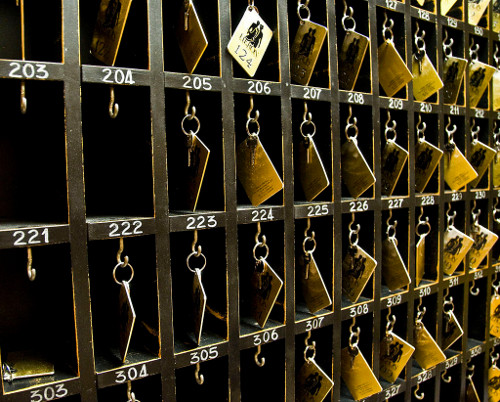
\includegraphics[width=0.95\textwidth]{/part01/onedoor.jpg}
  \begin{center}
    {\large ``One door, one key\ldots''}\par
    Foto di Silv3rFoX\par
    \url{http://www.flickr.com/photos/12030514@N08/2272118558/}\par
    Licenza: Creative Commons Attribution\par
  \end{center}
\clearpage
\cleardoublepage 
% (c) 2012 -2014 Dimitrios Vrettos - d.vrettos@gmail.com
% (c) 2014 Claudio Carboncini - claudio.carboncini@gmail.com
% (c) 2014 Daniele Masini - d.masini.it@gmail.com

\chapter{Numeri naturali}

\section{L'origine dei numeri}

L'origine del sistema dei numeri naturali si perde nella notte dei tempi. Non abbiamo
documenti sufficienti per capire come l'uomo li abbia costruiti o scoperti; è possibile
che il nostro sistema di numerazione sia nato contemporaneamente al linguaggio stesso
della specie umana. Sono stati ritrovati tronchi fossili risalenti a più di trentamila
anni fa, recanti delle incisioni a distanza regolare. In particolare, è stato ritrovato un
osso di babbuino, detto ``Osso di Ishango'' (figura \ref{fig:ishango})
\footnote{\url{http://it.wikipedia.org/wiki/Osso_d'Ishango}} in quanto è stato rinvenuto presso la città di
Ishango nel Congo tra il Nilo e il lago Edoardo, che riporta delle tacche disposte
in modo tale da farci pensare che rappresentino dei numeri o dei calcoli. L'osso risale a
un periodo tra il~$20\,000$~\aC\ e il~$18\,000$~\aC

\begin{wrapfloat}{figure}{r}{0pt}
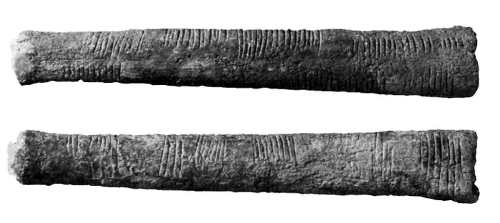
\includegraphics[scale=0.35]{/part01/chap01/fig001.png}
\caption{Osso di Ishango}
\label{fig:ishango}
\end{wrapfloat}
Possiamo immaginare che i pastori per contare i capi del proprio gregge, facessero delle
tacche su dei bastoni mano a mano che le pecore entravano nel recinto una alla volta: una
tacca per ogni pecora. Tuttavia, questo metodo di associazione uno ad uno (una tacca per
una pecora) non è efficace per greggi, o oggetti da contare, di grandi dimensioni. Si
immagini, per esempio, la difficoltà di tracciare cinquecento tacche su un bastone. È
possibile allora che per rappresentare numeri grandi si siano cominciati a usare simboli
specifici che richiamassero alla mente i numeri grandi e che contemporaneamente siano
state fissate alcune regole per associare questi simboli.

Sappiamo per certo che circa~6\,000 anni fa gli antichi Egizi scrivevano, incidendo sulla
pietra, i numeri utilizzando geroglifici per le potenze di~10:

% (c) 2012 Dimitrios Vrettos - d.vrettos@gmail.com
% Numeri egiziani
\begin{table}[!h]
  \begin{center}
    \begin{tabular}{ccccccc}
      \toprule
	\begin{hieroglyph}{\leavevmode \loneSign{\Aca GC/42/}}\end{hieroglyph} &  %
	\begin{hieroglyph}{\leavevmode \loneSign{\Aca GI/40/}}\end{hieroglyph} &%
	\begin{hieroglyph}{\leavevmode \loneSign{\Aca GD/84/}}\end{hieroglyph} &%
	\begin{hieroglyph}{\leavevmode \loneSign{\Aca GM/43/}}\end{hieroglyph} &%
	\begin{hieroglyph}{\leavevmode \loneSign{\Aca GV/32/}}\end{hieroglyph} &%
	\begin{hieroglyph}{\leavevmode \loneSign{\Aca GV/51/}}\end{hieroglyph}&%
	\begin{hieroglyph}{\leavevmode \loneSign{\Aca GZ/32/}}\end{hieroglyph}\\
      \midrule
	1\,000\,000   & 100\,000 & 10\,000 & 1\,000 & 100 & 10 & 1\\
      \bottomrule
    \end{tabular}
  \end{center}
\end{table}
\vspace{-4ex}
Ripetendo questi simboli è possibile scrivere, per esempio, il numero~$\np{3673}$ così:

\vspace{-2ex}% (c) 2012 Dimitrios Vrettos - d.vrettos@gmail.com
  \begin{center}
    \begin{hieroglyph}{\leavevmode \loneSign{\Aca GM/43/}\HinterSignsSpace
\loneSign{\Aca GM/43/}\HinterSignsSpace
\loneSign{\Aca GM/43/}\HinterSignsSpace
\Cadrat{\CadratLineI{\Aca GV/32/\hfill\Aca GV/32/\hfill\Aca GV/32/}\CadratLine{\Aca GV/32/\hfill\Aca GV/32/\hfill\Aca GV/32/}}\HinterSignsSpace
\Cadrat{\CadratLineI{{\Hsmaller\Hsmaller\Aca GV/51/}\hfill{\Hsmaller\Hsmaller\Aca GV/51/}\hfill{\Hsmaller\Hsmaller\Aca GV/51/}}\CadratLine{\Aca GV/51/\hfill\Aca GV/51/\hfill\Aca GV/51/\hfill\Aca GV/51/}}\HinterSignsSpace
\loneSign{\Aca GZ/32/}\HinterSignsSpace
\loneSign{\Aca GZ/32/}\HinterSignsSpace
\loneSign{\Aca GZ/32/}}\end{hieroglyph}
  \end{center}\vspace{-2ex}

I Romani usavano invece sette simboli con i quali, seguendo determinate regole,
rappresentavano qualunque numero. I simboli sono~$I=1$, $V=5$, $X=10$, $L=50$, $C=100$, $D=500$, $M=\np{1000}$.
La scrittura~$MM$ rappresenta il valore~$\np{1000}+\np{1000} = \np{2000}$, mentre~$VI$ rappresenta~$5+1=6$ ed invece~$IV$ rappresenta~$5-1=4$.

\section{Il sistema di numerazione decimale posizionale}
Il modo di scrivere i numeri dei Romani risultava piuttosto complicato sia nella scrittura
dei numeri sia nell'esecuzione dei calcoli. Il sistema tutt'oggi utilizzato per la scrittura dei numeri fa uso dei soli dieci simboli~0, 1, 2, 3, 4, 5, 6, 7, 8, 9, che vengono detti \emph{cifre}. Un numero è rappresentato da una sequenza ordinata di tali cifre (eventualmente anche ripetute).

Per rappresentare il numero dieci, che segue il~9, non si fa uso di un simbolo diverso ma si scrivono due cifre: il simbolo 1 e il simbolo 0 alla sua destra. Per chiarire questo metodo utilizziamo un pallottoliere (figura~\ref{fig:pallottoliere}) con aste verticali capaci di contenere fino a~9 dischetti: per rappresentare il numero~10 dispongo un dischetto nell'asta a sinistra e svuotando quella immediatamente alla sua destra: il numero dieci viene rappresentato dalla scrittura~10 che indica appunto 1 dischetto nella seconda asta (iniziando il conteggio da quella più a destra) e 0 in quella immediatamente a destra.

\begin{wrapfloat}{figure}{r}{0pt}
% (c) 2012 Dimitrios Vrettos - d.vrettos@gmail.com
% pallottoliere

\newcommand{\base}{%
  \filldraw[fill=black!90, draw=gray!80,rounded corners,shading=radial, inner color=white, outer color=gray!90]%
    (-2.4cm, -0.2cm) rectangle (2.4cm,0.4cm);
}

\newcommand{\aste}{%
  \fill[fill=black!90,rounded corners,shading=radial, inner color=white, outer color=gray!90]%
    (-1.25mm,3mm) rectangle (1.25mm,4.3cm);
}

\newcommand{\disco}{%
    \filldraw[fill=gray!20,draw=gray, rounded corners, shade,shading=radial, inner color=white, outer color=blue!50]%
      (-.6cm, .4cm) rectangle (.6cm,0.8cm);
}
\begin{tikzpicture}[scale=.7]
  \foreach \n/\a in {-15.25mm,0,15.25mm,36.75mm,52mm,67.25mm}{
    \begin{scope}[xshift=\a]
      \aste
    \end{scope}
  }

  \foreach \n/\x in {1/0cm,2/5.2cm}{%
    \begin{scope}[xshift=\x]
	\base
    \end{scope}
  }
  
  \foreach \n/\y in {0,.4cm,...,3.2cm}{%
    \begin{scope}[xshift=15.75mm,yshift=\y]
	\disco
    \end{scope}
  }   	
	
  \foreach \n/\z in {0}{%
    \begin{scope}[xshift=52mm,yshift=\z]
      \disco
    \end{scope}
  }

\end{tikzpicture}

\caption{Il pallottoliere}
\label{fig:pallottoliere}
\end{wrapfloat}

I dischetti sull'ultima asta rappresentano il numero~9; un dischetto sulla penultima
rappresenta il numero~10. Per rappresentare il numero cento si fa uso della scrittura~100.
Ovvero si sposta il numero~1 ancora a sinistra ponendo uno 0 nel posto lasciato vuoto.

Questo metodo rappresenta i numeri dando ad ogni cifra un peso differente a seconda della posizione che essa occupa all'interno della rappresentazione del numero stesso: ogni posizione occupata da una cifra vale 10 volte di più rispetto a quella che si trova immediatamente alla sua destra.
La rappresentazione di un numero è quella che si ottiene riportando il numero di dischetti presenti in ogni asta dell'abaco, uno accanto all'altro. Per esempio, se ci sono soltanto 3 dischetti nella terza asta il numero in cifre è~$300$, mentre la scrittura~$219$ indica 2 dischetti nella terza asta, 1 nella seconda e 9 nella prima.
Il sistema di numerazione che utilizziamo, detto \emph{sistema decimale}, si basa sulle potenze di~10 (sezione~\ref{sect:potenza}), che è la base dei pesi assegnati alle posizioni occupate dalle cifre.

Nel pallottoliere ciascuna asta indica una potenza di dieci. Il valore di un numero si ottiene moltiplicando ciascuna cifra per il suo peso e sommando i valori ottenuti.

Per esempio, tre dischetti nella terza asta rappresentano il numero~$~3\cdot 10^2=300$.
Il numero~$219$ si rappresenta tenendo conto di questa scrittura~$~2\cdot 10^2+1\cdot 10+9$.

Per quanto detto, il sistema di numerazione che usiamo è decimale o a base dieci, perché
utilizza dieci simboli (cifre) per rappresentare i numeri, e posizionale perché una stessa cifra
assume un peso (valore) diverso a seconda della posizione che essa occupa.

\section{I numeri naturali}

I primi numeri che abbiamo usato sin da bambini per contare gli oggetti o le persone si
chiamano \emph{numeri naturali}
\[ 0\text{,~}1\text{,~}2\text{,~}3\text{,~}4\text{,~}5\text{,~}6\text{,~}7\text{,~}8\text{,~}9\text{,~}10\text{,~}11\text{,~}12\text{,~}13\text{,~}\dots \]
L'insieme di tutti questi numeri si indica con la lettera~$\insN$.

Cosa hanno in comune le dita di una mano, con~5 mele, 5~penne, 5~sedie? Evidentemente
il numero~5. Una caratteristica cioè che è comune a tutti gli insiemi formati da~5
oggetti. Questa caratteristica può essere vista come un oggetto a sé stante, un oggetto
astratto di tipo matematico.

Ma i numeri naturali non servono solo per indicare quanti oggetti ci sono (aspetto
\emph{cardinale} del numero), vengono usati anche per rappresentare l'ordine con cui si
presentano gli oggetti, (aspetto \emph{ordinale}), l'ordine per esempio con cui i corridori
arrivano al traguardo: primo, secondo, terzo, \ldots

Nonostante i numeri naturali e le operazioni su di essi ci vengano insegnati fin da
piccoli, e nonostante l'umanità li usi da tempi antichissimi una loro piena comprensione
non è semplice, come dimostra il fatto che ancora oggi i matematici ne discutono. Il
dibattito su cosa siano i numeri e su cosa si fondano è stato particolarmente animato nei
primi decenni del $XX$~secolo, quando ne hanno discusso matematici e filosofi come Frege,
Peano, Russell, Hilbert e tanti altri. Oggi ci sono diversi punti di vista.

\subsection{Rappresentazione geometrica}
I numeri naturali possono essere rappresentati su una semiretta: si identifica il numero~0
con l'origine della semiretta, come verso di percorrenza si prende quello da sinistra
verso destra e come unità di misura un segmento~$\overline{AB}$. Si riporta questa unità di misura
più volte partendo dall'origine e a ogni passo si va al numero successivo.
\begin{center}
 % (c) 2012 Dimitrios Vrettos - d.vrettos@gmail.com

\begin{tikzpicture}
\begin{scope}[thick,font=\scriptsize]
	\draw[->] (0,0)  - -  (280pt,0) node[above]{$\insN$};
% 	\draw(1,-3pt) -- (1,3pt) node[below]{$1$};	
		\foreach \n in {0,1,2,...,9}{%
        	\draw (\n,-3pt) -- (\n,3pt)   node [below=5pt] {$\n$};}

		\draw[|-|]node [below=22pt]{$A$}(0,-20pt)--(29pt,-20pt) node[below=2pt]{$B$};

\end{scope}
\node [right,font=\scriptsize] at (+35pt,-20pt) {unit\`a};
\end{tikzpicture}

\end{center}

Ogni numero naturale si costruisce a partire dal numero~0 e passando di volta in volta al
numero successivo: 1 è il successore di~0, 2~è il successore di~1, 3~è il successore di~2,
ecc. Ogni numero naturale ha il successore e ogni numero, a eccezione di~0, ha il
precedente. L'insieme~$\insN$ ha~0 come elemento minimo e non ha un elemento massimo.

I numeri rappresentati sulla retta sono sempre più grandi man mano che si procede da
sinistra verso destra. Ogni numero è maggiore di tutti i suoi precedenti, quelli che
stanno alla sua sinistra, e minore di tutti i suoi successivi, quelli che stanno alla sua
destra. Tra i numeri naturali esiste quindi una \emph{relazione d'ordine}, che si rappresenta con i simboli di
\emph{disuguaglianza}~$\le$ (si legge ``minore o uguale a'') e~$\ge$ (si legge ``maggiore o uguale a'') o \emph{disuguaglianza stretta}~$<$ (si legge ``minore di'') e~$>$ (si legge ``maggiore di'').
Grazie a questo ordinamento, è sempre possibile confrontare due numeri naturali qualsiasi.

\begin{legge}[di tricotomia]
Dati due numeri naturali~$n$ e~$m$ vale sempre una delle seguenti tre relazioni: \quad $n<m$,\quad $n=m$,\quad $n>m$.
\end{legge}

\section{Operazioni con i numeri naturali}
\subsection{Addizione e moltiplicazione di numeri naturali}

Tra i numeri naturali è definita l'operazione di addizione come segue:

\begin{definizione}
Dati due numeri naturali~$n$ e~$m$, detti \emph{addendi}, l'operazione di \emph{addizione} associa ai
due addendi un terzo numero~$s$, detto \emph{somma}, che si ottiene partendo da~$n$ e procedendo
verso i successivi di~$n$ tante volte quante indica il secondo addendo~$m$.
\end{definizione}

L'operazione di addizione è indicata con il simbolo ``$+$'':
\begin{empheq}[box=\fbox]{equation*}
 n+m=s.
\end{empheq}
Ad esempio, se vogliamo eseguire la somma~$3+5$, dobbiamo partire da~3 e contare~5 numeri successivi:

% (c) 2012 Dimitrios Vrettos - d.vrettos@gmail.com

\begin{center}
 \begin{tikzpicture}[decoration={markings,mark=between positions 0.7 and .9 step 30pt with {\arrow{stealth}}}]
  \begin{scope}[thick,font=\scriptsize]
   \draw[->] (0,0)  - -  (280pt,0) node[above]{$\insN$};
    \foreach \c in {3,4,...,7}{%
     \draw[dotted, color=RedOrange,postaction={decorate}](\c,5pt)--(\c,5pt) arc (180:0:0.5 and 0.5);}
    \foreach \n in {0,1,2,...,9}{%	
     \draw (\n,-3pt) -- (\n,3pt)   node [below=5pt] {$\n$};}
  \end{scope}
 \end{tikzpicture}
\end{center}


\begin{definizione}
Dati due numeri naturali~$n$,~$m$, detti \emph{fattori}, l'operazione di
\emph{moltiplicazione} associa ai due fattori un terzo numero~$p$, detto \emph{prodotto},
che si ottiene sommando~$n$ addendi tutti uguali a~$m$.
\end{definizione}

L'operazione di moltiplicazione può essere indicata con diversi simboli:
\begin{empheq}[box=\fbox]{equation*}
n\times m=p\text{,}\qquad n\cdot m=p\text{,~}\qquad n\ast m=p.
\end{empheq}
Per eseguire la moltiplicazione~$4\cdot 2$ dobbiamo addizionare 4 volte 2, cioè~$2+2+2+2$, e otteniamo~8.

Le operazioni di addizione e moltiplicazione si dicono \emph{operazioni interne} all'insieme dei
numeri naturali, poiché, utilizzando numeri naturali, esse danno sempre come risultato un numero naturale.

 \vspazio\ovalbox{\risolvi \ref{ese:1.1}}

\subsection{Sottrazione e divisione di numeri naturali}

Diamo la seguente definizione:

\begin{definizione}
Dati due numeri naturali~$n$ e~$m$, il primo detto \emph{minuendo} e il secondo \emph{sottraendo}, si
dice \emph{differenza} il numero naturale~$d$, se esiste, che aggiunto ad~$m$ dà come somma~$n$.
\end{definizione}

L'operazione di sottrazione è indicata con il simbolo ``$-$'':
\begin{empheq}[box=\fbox]{equation*}
 n-m=d.
\end{empheq}

Per esempio, $7-5=2$ perché~$5+2=7$.

Non esiste invece la differenza tra~5 e~7, in quanto nessun numero naturale aggiunto a~7
può dare~5.

Ritornando alla rappresentazione dei numeri naturali sulla semiretta orientata, la
differenza tra i numeri~7 e~5 si può trovare partendo da~7 e procedendo a ritroso di~5
posizioni.

% (c) 2012 Dimitrios Vrettos - d.vrettos@gmail.com

\begin{center}
 \begin{tikzpicture}[decoration={markings,mark=between positions .3 and .5 step 30pt with {\arrowreversed{stealth}}}]
  \begin{scope}[thick,font=\scriptsize]
   \draw[->] (0,0)  - -  (280pt,0) node[above]{$\insN$};
    \foreach \c in {2,3,...,6}{%
     \draw[dotted, color=CornflowerBlue,postaction={decorate}](\c,5pt)--(\c,5pt) arc (180:0:0.5 and 0.5);}
    \foreach \n in {0,1,2,...,9}{%	
     \draw (\n,-3pt) -- (\n,3pt)   node [below=5pt] {$\n$};}
  \end{scope}
 \end{tikzpicture}
\end{center}


Diventa allora evidente perché non è possibile trovare la differenza tra~5 e~7, infatti
partendo dal~5 non è possibile andare indietro di~7 posizioni, poiché non è possibile
andare oltre il numero~0 che è il più piccolo dei numeri naturali.

% (c) 2012 Dimitrios Vrettos - d.vrettos@gmail.com

\begin{center}
 \begin{tikzpicture}[decoration={markings,mark=between positions .3 and .5 step 30pt with {\arrowreversed{stealth}}}]
  \begin{scope}[thick,font=\scriptsize]
   \draw[->] (0,0)  - -  (280pt,0) node[above]{$\insN$};
    \foreach \c in {-2,-1,...,4}{%
     \draw[dotted, color=CornflowerBlue,postaction={decorate}](\c,5pt)--(\c,5pt) arc (180:0:0.5 and 0.5);}
    \foreach \n in {0,1,2,...,9}{%	
     \draw (\n,-3pt) -- (\n,3pt)   node [below=5pt] {$\n$};}
  \end{scope}
 \end{tikzpicture}
\end{center}


Si può osservare allora che in~$\insN$ la sottrazione~$a-b$ è possibile solo se~$b\leq a$.

\begin{definizione}
Dati due numeri naturali~$n$ e~$m$, con~$m\neq0$, il primo detto \emph{dividendo} e il secondo
\emph{divisore}, si dice \emph{quoziente esatto} (o \emph{quoto}) un numero naturale~$q$, se esiste, che moltiplicato
per~$m$ dà come prodotto~$n$.
\end{definizione}

L'operazione di divisione può essere indicata con diversi simboli:
\begin{empheq}[box=\fbox]{equation*}
n \div m=q\text{,}\qquad n : m=q\text{,}\qquad n/m=q.
\end{empheq}

Se il quoziente esiste, il numero~$m$ si dice \emph{divisore} di~$n$ e che~$n$ è \emph{divisibile} per~$m$.

\begin{definizione}
Un numero naturale~$m$ si dice \emph{multiplo} di un numero naturale~$n$ se esiste un numero~$p$
che moltiplicato per~$n$ dà~$m$, cioè~$m=n\cdot p$.
\end{definizione}
\begin{exrig}

 \begin{esempio}
$12:3=4$ perché~$3\cdot 4=12$. Quindi,~12 è divisibile per~3;~3 è un divisore di~12;~12 è un multiplo di~3.
 \end{esempio}

 \begin{esempio}
20 è divisibile per~4 perché~$20:4=5$.
 \end{esempio}

 \begin{esempio}
7 è divisore di~35 perché~$35:7=5$.
 \end{esempio}

 \begin{esempio}
6 è multiplo di~3 perché~$6=2\cdot 3$.
 \end{esempio}

 \begin{esempio}
5 non è multiplo di~3 poiché non esiste alcun numero naturale che moltiplicato per~3 dà~5.
 \end{esempio}
\end{exrig}

\osservazione In~$\insN$ la divisione tra due numeri~$m$ e~$n$, è possibile solo se~$m$ è multiplo di~$n$.

\vspazio\ovalbox{\risolvi\ref{ese:1.2}}\vspazio

Come hai potuto notare dagli esercizi precedenti la divisione tra due numeri naturali non è sempre possibile.
Con i numeri naturali però è sempre possibile eseguire la divisione con il resto.

\begin{definizione}
 Dati due numeri naturali~$n$ e~$m$, con~$m\neq~0$, si dice \emph{quoziente} tra~$n$ e~$m$, il più grande
numero naturale~$q$ che moltiplicato per~$m$ dà un numero minore o uguale a~$n$. Si dice \emph{resto} della divisione
tra~$n$ e~$m$ la differenza~$r$ tra il dividendo~$n$ e il prodotto tra il divisore~$m$ e il quoziente~$q$.
\end{definizione}

In simboli:
\begin{empheq}[box=\fbox]{equation*}
n=m\cdot q + r\text{,}\qquad r=n-m\cdot q.
\end{empheq}

\begin{exrig}
 \begin{esempio}
 Nella divisione con resto tra~25 e~7 si ha quoziente~3 (infatti~$7\cdot 3=21$,
 mentre~$7\cdot 4=28$ supera il dividendo) e resto~4 (infatti~$25-21=4$).
 Pertanto si può scrivere~$25=7\cdot 3+4$.

 % (c) 2012 Dimitrios Vrettos - d.vrettos@gmail.com

\begin{center}
\begin{tikzpicture}

\draw[-](0,.4)--(0,-.9); % verticale
\draw[-](0,0)--(.4,0) ; %orizzontale
\draw (-.1,-.5) -- (-.6,-.5); % resto

\node (a) at (.2,.2) {7};
\node (b) at (.2,-.2) {3};
\node (c) at (-.3,.2) {25};
\node (d) at (-.3,-.2) {21};
\node (e) at (-.2,-.7){4};

\begin{scope}[font=\scriptsize]
  \draw  [<-] (.4,.2)--(.7,.2) node[right] {divisore};
  \draw  [<-] (.4,-.2)--(.7,-.2) node[right] {quoziente};
  \draw  [<-] (-.6,.2)--(-.9,.2) node[left] {dividendo};
  \draw  [<-] (-.6,-.7)--(-.9,-.7) node[left] {resto};
\end{scope}

\end{tikzpicture}

\end{center}

 \end{esempio}

 \begin{esempio}
 $0:2 =~0$.
 \end{esempio}

 \begin{esempio}
$1:2 =~0$ con resto~1.
 \end{esempio}

 \begin{esempio}
$5:2 =~2$ con resto~1.
 \end{esempio}
\end{exrig}

\osservazione Nella definizione di quoziente abbiamo sempre richiesto che il divisore sia diverso da zero. In effetti, se il divisore è~0 non c'è nessun numero che moltiplicato per~0 ci possa dare un dividendo diverso da zero.
Per esempio, nella divisione~$5:0$ dobbiamo ottenere un numero che moltiplicato per~0 dia~5; ciò non è
possibile in quanto qualsiasi numero moltiplicato per~0 dà~0.
Invece nella divisione~$0:0$ un qualsiasi numero è adatto come quoziente, infatti qualsiasi numero
moltiplicato per~0 dà~0 come prodotto.

Nel linguaggio matematico diciamo che una divisione del tipo~$n:0$, con~$n\neq~0$, è \emph{impossibile}; mentre la
divisione~$0:0$ è \emph{indeterminata}.

\begin{definizione}
 Dati due numeri naturali~$n$ e~$m$, con~$m\neq~0$, la \emph{divisione intera} tra $n$ e $m$ è l'operazione
che associa il più grande numero naturale~$q$ (il quoziente) per il quale si ha~$q\cdot m\le n$.
\end{definizione}

La divisione intera si indica con ``$\divint$'':
\begin{empheq}[box=\fbox]{equation*}
n \divint m = q\quad\text{(con resto }r\text{)}.
\end{empheq}

\begin{exrig}
 \begin{esempio}
$0 \divint 5=0$.
 \end{esempio}

 \begin{esempio}
$9 \divint 2=4$.
 \end{esempio}

 \begin{esempio}
$3\divint 5=0$.
 \end{esempio}

 \begin{esempio}
$3\divint 0 = $ non si può fare: la divisione intera per~0 non è possibile. 
 \end{esempio}
\end{exrig}

\begin{definizione}
 Dati due numeri naturali~$n$ e~$m$, con~$m\neq~0$, l'operazione che restituisce il resto della
divisione intera tra~$n$ e~$m$ si chiama \emph{modulo} di~$n$ rispetto a~$m$.
\end{definizione}

L'operazione di modulo viene indicata con ``$\bmod$'':
\begin{empheq}[box=\fbox]{equation*}
n\bmod{m} = r\quad\text{(dove }r\text{ è il resto di~~}n\divint m\text{)}.
\end{empheq}

\begin{exrig}
 \begin{esempio}
$0\bmod 5=0$.
 \end{esempio}

 \begin{esempio}
$9\bmod 5 =1$.
 \end{esempio}

 \begin{esempio}
$10\bmod 5=0$.
 \end{esempio}

 \begin{esempio}
$3\bmod 5=3$.
 \end{esempio}

 \begin{esempio}
$11\bmod 5=1$.
 \end{esempio}

 \begin{esempio}
$3\bmod 0=$ non si può fare.
 \end{esempio}
\end{exrig}

\ovalbox{\risolvii \ref{ese:1.2}, \ref{ese:1.3}, \ref{ese:1.4}, \ref{ese:1.5}, \ref{ese:1.6}}\vspazio

Ripassiamo l'algoritmo della divisione intera per numeri a più cifre; questa procedura risulterà particolarmente
utile nel seguito.

\begin{center}
 % (c) 2012 Dimitrios Vrettos - d.vrettos@gmail.com
\usetikzlibrary{matrix}

\begin{tikzpicture}
	\begin{scope}[every node/.style={anchor=base,row sep=1pt, column sep =-1pt, text depth=0pt, text height=6pt,text width=3pt}]%[font=\ttfamily]
 	\matrix (divisione) [matrix of nodes]
 	{%
 		&	3 & 2 & 7 &[.2cm] 2	&	3 &[.8cm] & 1 & 3 & 2 & 9 &[.2cm] 1 & 0 & 7 &[.8cm]   & 1 & 2	& 5	& 9 & 4 & 3 &[.2cm] 1 & 7 & 1\\
 	 |[gray]| -	& 2 & 3 &  	& |[blue]|1 & |[blue]|4 &  			|[gray]| -& 1 & 0 & 7 &  	  & |[blue]|1 & |[blue]|2	  &  	  & |[gray]|- & 1 & 1 	& 9 & 7 &  	&  	& |[blue]|7 & |[blue]|3 & |[blue]|6\\
 	   	&   	& 9 & 7 &  	&  	& 			  &	  & 2 & 5 & 9 &  	  &		  &  	 &  &     &  & 6 & 2 & 4 &  &  &  & \\
       &|[gray]|-  & 9 & 2 &  &  &  &|[gray]|  - & 2 & 1 & 4 &  &  &  &  &     &|[gray]| - & 5 & 1 & 3 &  &  &  & \\
      &  &  & |[red]|5 &  &  &  &   &  & |[red]|4 & |[red]|5 &  &  &  &  &     &  & 1 & 1 & 1 & 3 &  &  & \\
	 &  &  &  &  &  &  &   &  &  &  &  &  &  &  &     & |[gray]|- & 1 & 0 & 2 & 6 &  &  & \\
	& & & & |[white]|- & & &  & & & & |[white]|- & & & &    & & & & |[red]|8 & |[red]| 7 & & & \\
 	};
	\end{scope}
	% Prima divisione
	\draw(divisione-1-5.north west)--(divisione-2-5.south west);
	\draw(divisione-1-5.south west)--(divisione-1-6.south east);
	\draw(divisione-2-2.south west)--(divisione-2-3.south east);
	\draw(divisione-4-3.south west)--(divisione-4-4.south east);
	% Seconda divisione
	\draw (divisione-1-12.north west) -- (divisione-2-12.south west);
	\draw (divisione-1-12.south west) -- (divisione-1-14.south east);
	\draw(divisione-2-8.south west)--(divisione-2-10.south east);
	\draw (divisione-4-9.south west) -- (divisione-4-11.south east);
	% Terza divisione
	\draw (divisione-1-22.north west) -- (divisione-2-22.south west);
	\draw (divisione-1-22.south west) -- (divisione-1-24.south east);
	\draw (divisione-2-16.south west) -- (divisione-2-19.south east);
	\draw (divisione-4-18.south west) -- (divisione-4-20.south east);
	\draw (divisione-6-18.south west) -- (divisione-6-21.south east);
	% Frecce
	\draw[densely dotted,->] (divisione-1-4) -- (divisione-3-4);
	\draw[densely dotted,->] (divisione-1-11) -- (divisione-3-11);
	\draw[densely dotted,->] (divisione-1-20) -- (divisione-3-20);
	\draw[densely dotted,->] (divisione-1-21) -- (divisione-5-21);
	% Didascalie
	\node (a) [below=of divisione-7-5.north west] {(a)};
	\node (b) [below=of divisione-7-12.north west] {(b)};
	\node (c) [below=of divisione-7-21.north west] {(c)};
\end{tikzpicture}

\end{center}

\begin{enumeratea}
 \item $327:23=$ quoziente~14 e resto~5;
 \item $1\,329:107=$ quoziente~12 e resto~45;
 \item $125\,943:171=$ quoziente~736 e resto~87.
\end{enumeratea}

\ovalbox{\risolvi \ref{ese:1.7}}

\section{Proprietà delle operazioni}

\subsection{Proprietà commutativa}
Un'operazione ($\diamond$) gode della proprietà \emph{commutativa} se, cambiando l'ordine dei numeri sui quali essa va
eseguita, il risultato non cambia.

\begin{empheq}[box=\fbox]{equation*}
a\diamond b = b\diamond a.
\end{empheq}

La proprietà commutativa \emph{vale} per le seguenti operazioni:
\begin{description*}
 \item[addizione]~$a+b=b+a$. \quad Es.~$3+5=5+3=8$;
 \item[moltiplicazione]~$a\cdot b=b\cdot a$. \quad Es.~$3\cdot 5=5\cdot 3=15$.
\end{description*}

La proprietà commutativa \emph{non vale} per le seguenti operazioni:
\begin{description*}
 \item[sottrazione]~$a-b\neq b-a$. \quad Es.~$8-3=5\neq 3-8\:\text{ non si può fare in }\insN$;
 \item[divisione]~$a:b\neq b:a$. \quad Es.~$8:4=2\neq 4:8\:\text{ non si può fare in }\insN$;
 \item[divisione intera]~$a\divint b\neq b\divint a$. \quad Es.~$17\divint~5=3\neq~5\divint~17=0$;
 \item[modulo]~$a\bmod b\neq b\bmod a$. \quad Es.~$9\bmod~2=1\neq~2\bmod~9=2$;
 \item[potenza]~$a^b\neq b^a$. \quad Es.~$3^2=9\neq~2^3=8$.
\end{description*}

\subsection{Proprietà associativa}
Un'operazione ($\diamond$) gode della proprietà \emph{associativa} se, presi arbitrariamente tre numeri legati da due operazioni,
è indifferente da quale operazione si inizia, in quanto il risultato che si ottiene è sempre lo stesso.

\begin{empheq}[box=\fbox]{equation*}
(a\diamond b) \diamond c = a\diamond (b \diamond c).
\end{empheq}

La proprietà associativa \emph{vale} per le seguenti operazioni:
\begin{description*}
 \item[addizione]~$(a+b)+c=a+(b+c)$. \quad Es.~$(3+5)+2=3+(5+2)=10$;
 \item[moltiplicazione]~$(a\cdot b)\cdot c=a\cdot (b\cdot c)$. \quad Es.~$(3\cdot 5)\cdot 2=~3\cdot(5\cdot 2)=30$.
\end{description*}

La proprietà associativa \emph{non vale} per le seguenti operazioni:
\begin{description*}
 \item[sottrazione]~$(a-b)-c\neq a-(b-c)$. \quad Es.~$(10-5)-2=3\neq~10-(5-2)=7$;
 \item[divisione]~$(a:b):c\neq a:(b:c)$. \quad Es.~$(16:4):2=2\neq~16:(4:2)=8$;
 \item[divisione intera]~$(a\divint b)\divint c\neq a\divint(b\divint c)$. \\\quad Es.~$(17\divint~5)\divint~2=1\neq~17	\divint%
			 (5\divint2)=8$;
 \item[modulo]~$(a\bmod b)\bmod c\neq a\bmod(b\bmod c)$. \\\qquad Es.~$(17\bmod~7)\bmod~1=1$~$\neq~17\bmod(7\bmod2)=0$.
\end{description*}

\subsection{Elemento neutro}
Un'operazione ($\diamond$) ha un \emph{elemento neutro} $n$ se composto con qualsiasi altro numero lo lascia invariato, sia quando
il numero è a destra, sia quando è a sinistra dell'operatore.

\begin{empheq}[box=\fbox]{equation*}
a\diamond n = n\diamond a = a.
\end{empheq}

L'elemento neutro dell'addizione è~0, sia che si trovi a destra che a sinistra:
\[a+0=~0+a =a.\]
L'elemento neutro della moltiplicazione è~1, sia che si trovi a destra sia che si trovi a sinistra:
\[a\cdot 1 =~1\cdot a = a.\]
La divisione ha l'elemento neutro a destra, che è~1, ma non ha elemento neutro a sinistra:
\[a:1 = a \quad~(1:a\neq a\text{, \:se }a\neq~1).\]
In maniera analoga, anche la sottrazione ha l'elemento neutro~0 solo a destra:
\[a-0 = a \quad~(0-a\neq a\text{, \:se }a\neq~0).\]

\subsection{Proprietà distributiva}

La proprietà \emph{distributiva} coinvolge due operazioni differenti ($\diamond$ e $\star$). La proprietà distributiva di $\star$ rispetto a $\diamond$ è espressa in simboli:

\begin{empheq}[box=\fbox]{align*}
a \star (b \diamond c) &= a \star b \diamond a \star c\\
(a \diamond b) \star c &= a \star c \diamond b \star c.
\end{empheq}

\subsubsection{Proprietà distributiva della moltiplicazione}
\paragraph{Rispetto all'addizione}
Moltiplicare il risultato dell'addizione di più numeri per un altro numero dà lo stesso risultato che
moltiplicare ogni addendo per il fattore considerato e addizionare i prodotti ottenuti. Questa proprietà vale sia se la somma è a destra sia se è a sinistra.
\begin{flalign*}
 a\cdot(b+c) = a\cdot b +a\cdot c &\text{\quad Es.~}3\cdot(2+4) = 3\cdot 2+3\cdot 4=18\\
 (a+b)\cdot c = a\cdot c + b\cdot c &\text{\quad Es.~}(2+4)\cdot 3 = 2\cdot 3 + 4\cdot 3=18.
\end{flalign*}

\paragraph{Rispetto alla sottrazione}
In maniera analoga:
\begin{flalign*}
 a\cdot(b-c) = a\cdot b -a\cdot c &\text{\quad Es.~}6\cdot(10-4) = 6\cdot 10-6\cdot 4=36\\
 (a-b)\cdot c = a\cdot c - b\cdot c &\text{\quad Es.~}(10-4)\cdot 6 = 10\cdot 6- 4\cdot 6=36.
\end{flalign*}

\subsubsection{Proprietà distributiva della divisione}
\paragraph{Rispetto all'addizione}
Solo se le somme sono a sinistra:
\begin{flalign*}
 (a+b+c):d=a:d+b:d+c:d &\text{\quad Es.~}(20+10+5):5=20:5+10:5+5:5=7.
\end{flalign*}

Verifichiamo con un esempio che non vale la proprietà distributiva se le somme si trovano a destra:~$120:(3+5)$
Eseguendo prima l'operazione tra parentesi si ottiene correttamente~$120:8=15$. Se si prova ad applicare
la proprietà distributiva si ottiene~$120:3+120:5=40+24=64$. Il risultato corretto è il primo.

\paragraph{Rispetto alla sottrazione}
Solo se la sottrazione è a sinistra:
\begin{flalign*}
 (a-b):c=a:c-b:c &\text{\quad Es.~}(20-10):5=20:5-10:5=4-2=2.
\end{flalign*}

Se, però, la sottrazione è a destra:
\[120:(5-3)=120:2=60\neq~120:5-120:3=24-40=\:\text{ non si può fare in }\insN.\]

\begin{legge}[Annullamento del Prodotto]\label{legge:annullamento_del_prodotto}
 Il prodotto di due o più numeri naturali si annulla se e solo se almeno uno dei fattori è nullo.
%\[ a\cdot b=0\quad\Leftrightarrow\quad a=0\,\text{ oppure }\,b=0. \]
\end{legge}
In simboli:
\begin{empheq}[box=\fbox]{equation*}
a\cdot b=0\quad\Leftrightarrow\quad a=0\;\vee\;b=0.
\end{empheq}

\begin{proof}
La dimostrazione verrà fatta prima per l'implicazione diretta ($\Rightarrow$) e poi per quella inversa ($\Leftarrow$).
\begin{enumerate}
\item $a\cdot b = 0 \:\Rightarrow\: a = 0\;\vee\;b=0$~~si dimostra per assurdo.

Supponiamo che esistano due valori $a$ e $b$ entrambi non nulli, per i quali vale la condizione $a\cdot b = 0$. Poiché $b\neq 0$ possiamo dividere per $b$ le quantità a destra e a sinistra del simbolo di uguaglianza, mantenendo comunque verificata l'uguaglianza stessa. Quindi abbiamo $a\cdot b : b = 0 : b$. Visto che $(a\cdot b):c = a\cdot(b:c)$ e che qualunque numero diviso se stesso dà come risultato 1, la parte a sinistra del simbolo disuguaglianza è $a \cdot b : b = a \cdot 1 = a$. Poiché 0 diviso qualunque numero diverso da zero dà come risultato 0, la parte a destra dell'uguaglianza vale $0 : b = 0$. Dunque mettendo insieme i passaggi precedenti otteniamo $a = 0$, che contraddice l'ipotesi iniziale ($a$ e $b$ entrambi non nulli), cioè siamo arrivati ad un assurdo. Pertanto abbiamo dimostrato che $a\cdot b = 0 \:\Rightarrow\: a = 0\;\vee\;b=0$.

\item La dimostrazione dell'implicazione inversa ($a = 0\;\vee\;b=0 \:\Rightarrow\: a\cdot b = 0$) deriva direttamente dalla definizione dell'operazione di moltiplicazione. Infatti se $a = 0$, qualunque sia $b$ si ha $0\cdot b = 0$. Un ragionamento equivalente vale nel caso in cui $b=0$.
\end{enumerate}
\end{proof}

%questo è presente anche nella prima pagina del capitolo 14
Il matematico Carl Friedrich Gauss\footnote{matematico, astronomo e fisico tedesco (1777 - 1855).} fu un bambino prodigio. Si racconta che a nove anni il suo insegnante ordinò di fare la somma dei numeri da~$1$~a~$100$. Poco dopo Gauss diede la risposta esatta sorprendendo il suo insegnante. Probabilmente egli aveva scritto in una riga i numeri da~$1$~a~$100$ e nella riga sottostante i numeri da~$100$~a~$1$, notando che ogni colonna dava per somma $101$. Quindi, anziché sommare uno ad uno i numeri da 1 a 100, moltiplicando $100$ per $101$ e dividendo il risultato per~$2$ Gauss aveva ottenuto rapidamente la risposta: $100 \cdot 101 : 2=\np{5050}$.
\begin{center}
\begin{tabular*}{.75\textwidth}{@{\extracolsep{\fill}}*{10}{r}}
$1$&$2$&$3$&$4$&$5$&$\ldots$&$97$&$98$&$99$&$100$\\
$100$&$99$&$98$&$97$&$96$&$\ldots$&$4$&$3$&$2$&$1$\\
\midrule
$101$&$101$&$101$&$101$&$101$&$\ldots$&$101$&$101$&$101$&$101$\\
\end{tabular*}
\end{center}

\ovalbox{\risolvii \ref{ese:1.8}, \ref{ese:1.9}}

\section{Potenza}\label{sect:potenza}
La \emph{potenza} di un numero naturale è una moltiplicazione che ha tutti i fattori uguali.

\begin{definizione}
Dati due numeri naturali~$a$ e~$n$, con~$n>1$, il primo detto \emph{base} ed il secondo \emph{esponente}, la potenza di~$a$ con esponente~$n$ è il numero~$p$ che si ottiene moltiplicando fra loro~$n$ fattori tutti uguali ad~$a$.
Si scrive~$a^n=p$ e si legge ``\emph{$a$ elevato a~$n$ uguale a~$p$}''.
\end{definizione}

Per esempio,~$5^3=5\cdot~5\cdot~5=125$.
\begin{center}
 % (c) 2012 Dimitrios Vrettos - d.vrettos@gmail.com
\begin{tikzpicture} 
  \node (esp) at (0,0) {$5^3=\underbrace{5\cdot 5\cdot 5}_{3 \text{ volte}} = 125$};
\begin{scope}[font=\scriptsize]
  \draw[<-]  (-1,.5)--(-0.8,.7) node[right] {esponente};
  \draw[->]  (-1.6,-.1)--(-1.4,.1) node[below left=.2] {base};
  \draw[<-]  (1.4,.1)--(1.6,-.1) node[below right] {potenza };
\end{scope}
\end{tikzpicture}

\end{center}

Quindi, in simboli
\begin{empheq}[box=\fbox]{equation*}
a^n = \underbrace{a\cdot a\cdot \ldots{} \cdot a}_{n \text{ volte}}
\end{empheq}

Per completezza, alla definizione precedente vanno aggiunti i seguenti casi particolari:
\begin{empheq}[box=\fbox]{align*}
 a^1&=a\text{,}\\
 a^0&=1\quad \text{se }a\neq~0\text{,}\\
 0^0&=\text{non ha significato.}
\end{empheq}

Queste definizioni trovano giustificazione nelle proprietà delle potenze.

\subsection{Proprietà delle potenze}

 \paragraph{I} Il prodotto di due potenze con la stessa base è uguale a una potenza che ha
 per base la stessa base e per esponente la somma degli esponenti.
 \begin{empheq}[box=\fbox]{equation*}
 a^n\cdot a^m=a^{n+m}
 \end{empheq}
 \[ 2^5\cdot 2^6=2^{5+6}=2^{11}.\]

La proprietà segue da questa osservazione:
\[ a^n\cdot a^m = \underbrace{(a\cdot a\cdot\ldots\cdot a)}_{n\text{ volte}}\cdot%
 \underbrace{(a\cdot a\cdot a\cdot\ldots\cdot a)}_{m\text{ volte}}
 =\underbrace{(a\cdot a\cdot a\cdot a\cdot a\cdot\ldots\cdot a\cdot a)}_{n+m\text{ volte}}%
 =a^{n+m}.\]

\paragraph{II} Il quoziente di due potenze con la stessa base, la prima con esponente
maggiore o uguale all'esponente della seconda, è uguale a una potenza che
ha per base la stessa base e per esponente la differenza degli esponenti.

 \begin{empheq}[box=\fbox]{equation*}
 a^n:a^m=a^{n-m}
 \end{empheq}
\[4^5:4^3=4^{5-3}=4^2.\]

La proprietà segue da questa osservazione:
\begin{align}
 a^n: a^m &= \underbrace{(a\cdot a\cdot\ldots\cdot a)}_{n\text{ volte}}:%
 \underbrace{(a\cdot a\cdot a\cdot\ldots\cdot a)}_{m\text{ volte}}\label{eq:pot_quoz1}\\
 &=\underbrace{(a:a)\cdot(a:a)\cdot\ldots\cdot(a:a)}_{n\text{ volte}}\cdot%
 \underbrace{(a\cdot a\cdot a\cdot\ldots\cdot a)}_{n-m\text{ volte}}\label{eq:pot_quoz2}\\%
 &=a^{n-m}.
\end{align}
Il passaggio dalla \ref{eq:pot_quoz1} alla \ref{eq:pot_quoz2} avviene per via della proprietà invariantiva della divisione.
\paragraph{III} La potenza di una potenza è uguale a una potenza che ha la base della prima
potenza e per esponente il prodotto degli esponenti.

 \begin{empheq}[box=\fbox]{equation*}
 (a^n)^m=a^{n\cdot m}
 \end{empheq}
\[(6^2)^5=6^{2\cdot 5}=6^{10}. \]

La proprietà segue da questa osservazione:

\[ (a^n)^m =\overbrace{a^n\cdot a^n\cdot\ldots\cdot a^n}^{m\text{ volte}}%
 =\overbrace{\underbrace{(a\cdot a\cdot\ldots\cdot a)}_{n\text{ volte}}\cdot%
	 \underbrace{(a\cdot a\cdot\ldots\cdot a)}_{n\text{ volte}}\cdot\ldots\cdot%
	 \underbrace{(a\cdot a\cdot\ldots\cdot a)}_{n\text{ volte}}}^{m\text{ volte}}%
	 =a^{n\cdot m}.\]

\paragraph{IV} Il prodotto di potenze con lo stesso esponente è
uguale al prodotto delle potenze dei singoli fattori.

 \begin{empheq}[box=\fbox]{equation*}
 (a\cdot b)^n=a^n\cdot b^n
 \end{empheq}
\[(2\cdot 5)^8=2^8\cdot 5^8. \]

La proprietà segue da questa osservazione:
\[(a\cdot b)^n=\underbrace{(a\cdot b)\cdot(a\cdot b)\cdot\ldots\cdot(a\cdot b)}_{n\text{ volte}}%
	 =\underbrace{(a\cdot a\cdot\ldots\cdot a)}_{n\text{ volte}}\cdot%
	 \underbrace{(b\cdot b\cdot\ldots\cdot b)}_{n\text{ volte}}%
	 =a^n\cdot b^n.\]

\paragraph{V} La potenza di un quoziente è uguale al quoziente delle potenze dei singoli
fattori.

 \begin{empheq}[box=\fbox]{equation*}
 (a:b)^n=a^n:b^n
 \end{empheq}
\[(4:2)^8=4^8:2^8. \]

Le definizioni dei casi particolari di potenze si giustificano nel seguente modo:
\begin{align*}
 &a^0=a^{5-5}=a^5:a^5=1,\\
 &a^1=a^{5-4}=a^5:a^4=a.
\end{align*}
Alla potenza~$0^0$ non si assegna nessun valore perché applicando la definizione di~$a^0$ si dovrebbe avere~1;
applicando la definizione~$0^a$ si dovrebbe avere~0.

\ovalbox{\risolvii \ref{ese:1.10}, \ref{ese:1.11}, \ref{ese:1.12}, \ref{ese:1.13}, \ref{ese:1.14}}\vspazio

\subsection{Cenni sull'estrazione di radice}

L'operazione inversa dell'elevazione a potenza è l'estrazione di \emph{radice}.

\begin{definizione}
Dati due numeri naturali~$a$ e~$n$ (con~$n>1$) si definisce \emph{radice}~$n$-esima di~$a$ il numero~$r$ tale che moltiplicando tra loro~$n$ fattori tutti uguali a~$r$ si ottiene come risultato~$a$.
\end{definizione}

In simboli:
\begin{empheq}[box=\fbox]{equation*}
\sqrt[n]{a} = r.%\quad\text{se}\quad r^n=a.
\end{empheq}

Per esempio~$\sqrt[3]{64} = 4$ poiché $4^3=4\cdot 4\cdot 4 = 64$.

\begin{exrig}
 \begin{esempio}
$\sqrt[5]{32} = 2$,~~infatti $2^5 = 2\cdot 2\cdot 2\cdot 2\cdot 2 = 32$.
 \end{esempio}

 \begin{esempio}
$\sqrt[3]{125} = 5$,~~infatti $5^3 = 5\cdot 5\cdot 5 = 125$.
 \end{esempio}

 \begin{esempio}
$\sqrt[4]{81} = 3$,~~infatti $3^4 = 3\cdot 3\cdot 3\cdot 3 = 81$.
 \end{esempio}

 \begin{esempio}
$\sqrt[7]{1} = 1$,~~infatti $1^7 = 1\cdot 1\cdot 1\cdot 1\cdot 1\cdot 1\cdot 1 = 1$.
 \end{esempio}
\end{exrig}

Particolare importanza riveste la radice con $n=2$, detta anche \emph{radice quadrata}. Ad esempio, la radice quadrata di 25 è 5, cioè $\sqrt[2]{25} = 5$, poiché infatti~$5^2 = 5\cdot 5=25$, e anche $\sqrt[2]{49} = 7$ ($7^2=49$). L'uso della radice quadrata è talmente predominante in matematica rispetto a quelle di ordine superiore (quelle con $n>2$) che nel caso in cui l'indice $n$ della radice non sia specificato si sottintende il valore 2: cioè $\sqrt{9} = \sqrt[2]{9} = 3$.


\section{Numeri Primi}

Osserva il seguente schema
\[\fbox{18}\quad\xrightarrow[\text{è divisibile per}]{\text{è multiplo di}}\quad \fcolorbox{gray}{grigio80}{6}\quad%
 \xrightarrow[\text{è divisore di}]{\text{è sottomultiplo di}}\quad \fbox{18}
\]
In esso sono descritte alcune caratteristiche del numero~18 e i suoi legami con il numero~6.

\begin{definizione}
 Chiamiamo \emph{divisore proprio} di un numero un suo divisore diverso dal numero stesso e dall'unità.
\end{definizione}

Osserva ora il seguente schema
\[\fbox{31}\quad\xrightarrow[\text{è divisibile per}]{\text{è multiplo di}}\quad \fcolorbox{gray}{grigio80}{\vphantom{3}\ldots}\quad%
 \xrightarrow[\text{è divisore di}]{\text{è sottomultiplo di}}\quad \fbox{31}
\]
Nella casella centrale, al posto dei puntini, puoi inserire soltanto i numeri~31 o~1.

\begin{definizione}
 Un numero~$p>1$ si dice \emph{primo} se è divisibile solo per se stesso e per l'unità. Un numero naturale maggiore di~1 non primo si dice \emph{composto}.
\end{definizione}

Per come sono stati definiti i numeri primi e quelli composti si ha:

\begin{multicols}{3}
\noindent~0 non è primo né composto;\\
1 non è primo né composto;\\
2 è primo;\\
3 è primo;\\
4 è composto;\\
5 è primo;\\
6 è composto;\\
7 è primo;\\
8 è composto;\\
9 è composto;\\
10 è composto;\\
11 è primo;\\
12 è composto;\\
13 è primo.\\
\ldots
\end{multicols}

\begin{exrig}
 \begin{esempio}
 Per verificare se~31 è primo, calcolo il valore approssimato~$\sqrt{31}\simeq\np{5,5}$ e verifico se è divisibile
per i numeri primi~$\le5$, cioè~2,~3 e~5. 31 non è divisibile per~2 in
quanto è dispari, non è divisibile per~3 poiché la somma delle sue cifre è~4 (che non è divisibile per~3) e
non è divisibile per~5 in quanto non finisce per~0 o~5 (sezione \ref{sect:criteri_divisibilita}). Quindi 31 è primo.
 \end{esempio}

 \begin{esempio}
 Per verificare se~59 è un numero primo calcolo~$\sqrt{59}\simeq\np{7,6}$ e verifico se~59 è divisibile per un
numero primo~$\le~7$, cioè per~2,~3,~5 e~7. Eseguendo le divisioni si vede che~59 non è divisibile
per nessuno di questi numeri, quindi è primo.
 \end{esempio}
\end{exrig}

\osservazione Un numero è primo quando non è divisibile per nessun numero primo compreso tra~2 e
la radice quadrata del numero stesso.

\vspazio\ovalbox{\risolvii \ref{ese:1.15}, \ref{ese:1.16}}


\section{Criteri di divisibilità}\label{sect:criteri_divisibilita}

Per verificare se un numero è divisibile per i primi numeri interi si possono applicare i seguenti criteri di
divisibilità.

\paragraph{Divisibilità per~2} Un numero è divisibile per~2 se e solo se la sua ultima cifra, quella delle unità,
è un numero pari, cioè è~0,~2,~4,~6,~8.

\begin{itemize*}
 \item \np{1236} finisce per~6 quindi è divisibile per~2;
 \item \np{109230} finisce per~0 quindi è divisibile per~2;
 \item \np{10923} finisce per~3 quindi non è divisibile per~2.
\end{itemize*}

\paragraph{Divisibilità per~3} Un numero è divisibile per~3 se e solo se la somma delle cifre che lo
compongono è divisibile per~3.
\begin{itemize*}
 \item 24 è divisibile per~3, infatti la somma delle sue cifre è~$2+4=6$, dato che~6 è divisibile per~3
anche~24 è divisibile per~3;
 \item \np{1236} è divisibile per~3, infatti la somma delle sue cifre è~$1+2+3+6=12$;~12~è divisibile per~3
dato che la somma delle sue cifre è~$1+2=3$, quindi anche~\np{1236} è divisibile per~3;
 \item 31 non è divisibile per~3, infatti la somma delle sue cifre è~$3+1=4$, dato che~4 non è
divisibile per~3 neanche~31 è divisibile per~3.
\end{itemize*}

\paragraph{Divisibilità per~5} Un numero è divisibile per~5 se la sua ultima cifra è~0 o~5.
\begin{itemize*}
 \item \np{1230} finisce per~0 quindi è divisibile per~5;
 \item \np{59235} finisce per~5 quindi è divisibile per~5;
 \item \np{109253} finisce per~3 quindi non è divisibile per~5;
 \item \np{5556} finisce per~6 quindi non è divisibile per~5.
\end{itemize*}

\paragraph{Divisibilità per~7} Un numero (maggiore di~10) è divisibile per~7 se la differenza (in valore assoluto\footnote{il \emph{valore assoluto} è trattato a pagina~\pageref{def:valass}.})
fra il valore ottenuto dal numero stesso togliendo la cifra delle unità e il doppio della cifra delle unità è~7 o un
multiplo di~7.
\begin{itemize*}
 \item 252 è divisibile per~7, infatti~$ \valass{25−2\cdot 2}=21$ è multiplo di~7;
 \item 49 è divisibile per~7, infatti~$\valass{4−2\cdot 9}=14$ è multiplo di~7;
 \item 887 non è divisibile per~7, infatti~$\valass{88−2\cdot 7}=74$ non è divisibile per~7.
\end{itemize*}

\paragraph{Divisibilità per~11} Un numero è divisibile per~11 se e solo se la differenza, in valore assoluto, fra la
somma delle cifre di posto pari e la somma delle cifre di posto dispari è~0,~11~o un multiplo di~11.
\begin{itemize*}
 \item 253 è divisibile per~11, infatti~$\valass{5-(2+3)}=0$;
 \item \np{9482} è divisibile per~11, infatti~$\valass{(9+8)−(4+2)}=11$;
 \item 887 non è divisibile per~11, infatti~$\valass{8-(8+7)}=7$.
\end{itemize*}

\ovalbox{\risolvii \ref{ese:1.17}, \ref{ese:1.18}}


\section{Scomposizione in fattori primi}

Scomporre in fattori (o fattorizzare) un numero significa scriverlo come prodotto di altri numeri naturali.

\begin{teorema}[fondamentale dell'aritmetica]\label{th:fondamentale_dell_aritmetica}
 Ogni numero naturale~$n>1$ si può scrivere in modo unico come prodotto di numeri primi.
\end{teorema}

%\begin{proof}
%La dimostrazione sarà effettuata in più fasi. Dapprima (punti 1 e 2) procederemo col dimostrare la possibilità di scrivere un numero sotto forma di prodotto di numeri primi (fattorizzazione). Quindi (punto 3) dimostreremo che tale fattorizzazione è unica.
%
%\begin{enumerate}
%\item \emph{Dimostriamo per induzione che ogni numero è divisibile per un numero primo o è primo esso stesso.}
%
%Il numero 2 è primo. Supponiamo che ogni numero da 2 a $n$ sia primo o divisibile per un numero primo e dimostriamolo per $n+1$.
%
%Considerando $n+1$ si hanno due possibilità:
%\begin{itemize*}
%\item $n+1$ è primo.
%\item $n+1$ non è primo, quindi è divisibile per un numero $a$ compreso tra 2 e $n$, e per l'ipotesi induttiva o $a$ è primo oppure è divisibile per un numero primo $p$. Quindi lo sarà anche $n+1$.
%\end{itemize*}
%Pertanto $n+1$ è divisibile per un numero primo o è esso stesso un numero primo.
%
%\item \emph{Dimostriamo per induzione che ogni numero è scomponibile in fattori primi.}
%
%Il numero 2 è già banalmente fattorizzato. Supponiamo che ogni numero da 2 a $n$ si possa scrivere come prodotto di numeri primi e dimostriamo che questo vale anche per $n+1$.
%
%Considerando $n+1$ si hanno due possibilità:
%\begin{itemize*}
%\item $n+1$ è primo, quindi già fattorizzato.
%\item $n+1$ non è primo, quindi divisibile per un primo $p$ (per quanto dimostrato al punto 1). Si consideri il numero $m=(n+1):p$ che è minore di $n+1$ e quindi, per l'ipotesi induttiva, può essere scomposto in un prodotto di numeri primi e pertanto lo è anche $n+1=m\cdot p$.
%\end{itemize*}
%
%Dunque, ogni numero è scomponibile in fattori primi.
%
%\item \emph{Dimostriamo adesso, per assurdo, che se un numero ammette una scomposizione in fattori primi questa è unica.}
%
%Si supponga che esistano dei numeri scomponibili in fattori primi in più di un modo. Sia $m$ il numero più piccolo tra essi. Siano inoltre (\ref{eq:num_primi_scomp1}) e (\ref{eq:num_primi_scomp2}) due sue diverse fattorizzazioni
%
%\begin{equation}\label{eq:num_primi_scomp1}
%m = p_1 \cdot p_2 \cdot \ldots \cdot p_s
%\end{equation}
%\begin{equation}\label{eq:num_primi_scomp2}
%m = q_1 \cdot q_2 \cdot \ldots \cdot q_t
%\end{equation}
%
%\noindent dove i numeri $p_1$,\ldots,$p_s$ e $q_1$,\ldots,$q_t$ sono primi ma differenti tra loro, ovvero $\forall i,j \; p_i \neq q_j$ (se ci fosse un fattore primo $p_h=q_k$ potremmo dividere $m$ per tale fattore ottenendo così un numero $m' < m$ che avrebbe anch'esso due fattorizzazioni distinte, riconducendoci così al caso considerato), sebbene all'interno di ogni fattorizzazione possano comunque essere presenti fattori ripetuti.
%Dunque $p_1\neq q_1$ e, senza perdita di generalità, possiamo supporre che $p_1 < q_1$.
%
%Sia
%\begin{equation}\label{eq:num_primi_scomp3}
%n = (q_1-p_1)\cdot q_2 \cdot \ldots \cdot q_t.
%\end{equation}
%Si ha $n < m$ dato che, per la proprietà distributiva della moltiplicazione rispetto all'addizione, l'uguaglianza precedente si può scrivere come
%\begin{equation}\label{eq:num_primi_scomp4}
%n = q_1\cdot q_2\cdot \ldots \cdot q_t - p_1\cdot q_2\cdot \ldots\cdot q_t = m - p_1\cdot q_2\cdot \ldots \cdot q_t < m.
%\end{equation}
%
%Se il primo fattore di $n$, $q_1-p_1$, non fosse primo lo potremo fattorizzare ottenendo così una nuova fattorizzazione di $n$ che non ammetterebbe $p_1$ tra i suoi fattori. Infatti, per quanto ipotizzato precedentemente, $p_1$ è diverso da $q_1$, $q_2$, \ldots, $q_t$, inoltre esso non può comparire nell'eventuale fattorizzazione di $q_1-p_1$, poiché se ciò accadesse significherebbe che $q_1$ è divisibile per $p_1$ (infatti $q_1-p_1= p_1\cdot a \:\Rightarrow\: q_1 = p_1\cdot(1+a)$), il che non è possibile in quanto per ipotesi $q_1$ è un numero primo. Dunque $q_1-p_1$ è primo.
%
%Considerando l'ultima uguaglianza della (\ref{eq:num_primi_scomp4}) e sostituendo in essa $m$ con la (\ref{eq:num_primi_scomp1}) otteniamo
%
%\begin{equation}\label{eq:num_primi_scomp5}
%n= p_1 \cdot p_2 \cdot \ldots\cdot p_s-p_1\cdot q_2 \cdot \ldots \cdot q_t \:\Rightarrow\: n = p_1\cdot(p_2\cdot \ldots \cdot p_s- q_2\cdot \ldots\cdot q_t)
%\end{equation}
%
%In qualunque modo sia scomponibile il secondo fattore della (\ref{eq:num_primi_scomp5}), si ha una fattorizzazione di $n<m$ che contiene $p_1$ e che è quindi diversa da quella della (\ref{eq:num_primi_scomp3}), contrariamente all'ipotesi che $m$ sia il numero più piccolo che ammette più di una fattorizzazione.
%\end{enumerate}
%Dunque la scomposizione di un numero in fattori primi è unica.
%\end{proof}

\begin{exrig}
 \begin{esempio}
 Scomporre in fattori primi il numero~630.
 \begin{center}
% % (c) 2012 Dimitrios Vrettos - d.vrettos@gmail.com
\begin{tikzpicture}
\begin{scope}[font=\ttfamily]
\matrix (scomposizione)[matrix of nodes]{
	6&3&0 & 2\\
	3&1&5 & 3\\
	1&0&5 & 3\\
	&3&5 &5\\
	&&7 & 7\\
	&&1 & \\
};
\end{scope}
 \draw(scomposizione-1-3.north east)--(scomposizione-6-3.south east);

\node (a) [right=of scomposizione-1-4.east] {630 \`e divisibile per 2 perch\'e l'ultima cifra \`e pari;};
\node (b) [right=of scomposizione-2-4.east] {315 \`e divisibile per 3, la somma delle sue cifre \`e 9 divisibile per 3;};
\node (c) [right=of scomposizione-3-4.east] {105 \`e divisibile per 3, la somma delle sue cifre \`e 6 divisibile per 3;};
\node (d) [right=of scomposizione-4-4.east] {35 \`e divisibile per 5 perch\'e l'ultima cifra \`e 5;};
\node (e) [right=of scomposizione-5-4.east] {7 \`e un numero primo.};
\end{tikzpicture}

 \begin{tabular}{r|l@{\hspace{15mm}}l}
 	630 & 2 & 630 è divisibile per 2 perché l'ultima cifra è pari;\\
	315 & 3 & 315 è divisibile per 3 (la somma delle sue cifre è 9, divisibile per 3);\\
	105 & 3 & 105 è divisibile per 3 (la somma delle sue cifre è 6, divisibile per 3);\\
	35 & 5 & 35 è divisibile per 5 perché l'ultima cifra è 5;\\
	7 & 7 & 7 è un numero primo.\\
	1 & \\
 \end{tabular}
 ~$630=2\cdot3^2\cdot5\cdot7.$
 \end{center}
 \end{esempio}
\end{exrig}

In generale, un numero può essere scomposto in fattori in più modi. Per esempio,~$12=3\cdot 4$,
ma anche~$12=6\cdot2$. Il teorema fondamentale dell'aritmetica ci assicura che, se si scompone un numero in fattori primi,
questa scomposizione è unica, a meno dell'ordine con cui si scrivono i fattori. Tornando all'esempio
precedente~$12=~2^2\cdot 3$ è l'unico modo in cui il~12 si può scomporre in fattori primi, a meno che non si
scambino di posto i fattori~$12=3\cdot 2^2$.

I numeri primi sono quindi i mattoni fondamentali dell'aritmetica, poiché gli altri numeri naturali possono essere ottenuti, in maniera univoca, come prodotto di primi.

Sebbene al crescere dei valori considerati i numeri primi diventino sempre più radi, essi sono comunque infiniti, come affermò Euclide\footnote{matematico e scienziato della Grecia antica (367 \aC{} ca. - 283 \aC).} con il seguente teorema che porta il suo nome:
\begin{teorema}[di Euclide]
I numeri primi sono infiniti.
\end{teorema}

\begin{proof}
Il teorema può essere dimostrato per assurdo.
Supponiamo infatti che i numeri primi siano un numero finito, cioè siano, ordinati dal più piccolo al più grande, $p_1$, $p_2$, \ldots{}, $p_n$. Si consideri il numero $a=p_1\cdot p_2\cdot \ldots{}\cdot p_n+1$. Per com'è stato scelto, $a$ non è divisibile per nessuno dei numeri $p_1$, $p_2$, \ldots{}, $p_n$ poiché la divisione per qualunque di essi darà sempre come resto 1. Quindi o $a$ è un numero primo maggiore di $p_n$ oppure, per il teorema fondamentale dell'aritmetica (pagina \pageref{th:fondamentale_dell_aritmetica}), è divisibile per un numero primo $p^*$ differente da $p_1$, $p_2$, \ldots{}, $p_n$. In entrambi i casi si ha una contraddizione con l'ipotesi iniziale, cioè che i numeri primi siano un numero finito, poiché per come è stato scelto, $a$ implica l'esistenza di un numero primo che non è nell'elenco ipotizzato $p_1$, $p_2$, \ldots, $p_n$. Quindi i numeri primi sono infiniti.
\end{proof}

\ovalbox{\risolvii \ref{ese:1.19}, \ref{ese:1.20}}
%\vspazio\ovalbox{\risolvi \ref{ese:1.17}}


\subsection{Numeri primi e crittografia}

Il problema legato alla scomposizione in fattori primi è di notevole interesse per i matematici, poiché non è ancora stato individuato un meccanismo che permette di stabilire se un numero sia primo o meno\footnote{si tratta della dimostrazione dell'ipotesi di Riemann, uno dei 7 \emph{Millennium problems} elencati il 24 maggio 2000, ovvero questioni matematiche ad oggi (2014) ancora non dimostrate (tranne una). Vista l'enorme difficoltà nel riuscire nell'intento, il Clay Mathematics Institute ha messo in palio un milione di dollari per la dimostrazione di ognuna di esse (v.~\url{http://it.wikipedia.org/wiki/Problemi_per_il_millennio}).}, se non quello di provare a dividerlo per tutti i numeri minori o uguali alla sua radice quadrata, procedura che diventa sempre più lunga man mano che le cifre che compongono il numero da verificare aumentano. Per questo motivo l'utilizzo di valori che siano il prodotto di numeri primi con un numero elevato di cifre è ciò che sta alla base della moderna crittografia, ovvero dei sistemi per la cifratura dei messaggi.

Consideriamo un semplice esempio che può chiarire come funziona il meccanismo di base per inviare messaggi segreti.

Alice deve inviare la sua password, la parola ``BACI'', a suo fratello Bruno. Alice trasforma la parola in numeri secondo la semplice regola A=1, B=2, C=3, I=9 (assegnando ad ogni lettera il numero cardinale corrispondente alla sua posizione nell'alfabeto). Il messaggio diventa così~$ \np{2139} $. Alice moltiplica questo numero per un numero primo ``segreto'' (che conosce solo lei) $\np{26417}$ e ottiene $\np{2139} \cdot \np{26417}=\np{56505963}$ e invia quest'ultimo numero a Bruno. Chiunque intercetti questo numero non è in grado di individuare la password in chiaro.

Quando Bruno riceve il numero $ \np{56505963} $ lo moltiplica per un suo numero primo ``segreto'' (che conosce solo lui) $\np{43969}$ ottenendo $\np{5650593} \cdot \np{43969}=\np{2484510687147}$ e lo invia nuovamente ad Alice.

Quando Alice riceve il numero lo divide per il suo numero primo $\np{2484510687147} : \np{26417} = \np{94049691}$ e quindi lo rispedisce a Bruno,
A questo punto Bruno divide il numero ricevuto per il suo numero primo segreto ottenendo $\np{94049691} : \np{43969} = \np{2139}$. Conoscendo il meccanismo di codifica (relazione tra i numeri e le lettere dell'alfabeto  2=B, 1=A, 3=C, 9=I) Bruno può dunque ricostruire la password ``BACI''.

In realtà, i sistemi per lo scambio di messaggi cifrati oggi utilizzati per mezzo dei computer si basano su meccanismi leggermente differenti che evitano il doppio invio di messaggi tra Alice e Bruno. I meccanismi sono essenzialmente due: il primo è detto \emph{a chiave simmetrica}, in cui sia Alice che Bruno condividono il numero segreto con il quale viene cifrato il messaggio e quindi entrambi possono codificarlo e decodificarlo autonomamente; il secondo, un po' più complesso ma che dà le stesse garanzie del doppio invio di messaggi (nessuna condivisione del numero segreto tra gli interlocutori), viene chiamato \emph{a chiave asimmetrica} e si basa sull'utilizzo di un numero segreto ed un numero pubblico da condividere con l'interlocutore.

Va comunque sottolineato il fatto che la robustezza del meccanismo di cifratura sta nella difficoltà intrinseca della fattorizzazione di numeri molto grandi. Ciò non significa che i messaggi rimarranno segreti per sempre: prima o poi saranno decifrati visto che la velocità di calcolo dei computer è sempre in aumento. Per cercare di rendere il processo di decifratura più arduo si possono scegliere chiavi di cifratura composte da numeri primi sempre più grandi.


\section{Massimo Comune Divisore e minimo comune multiplo}

\label{def:mcd}
\begin{definizione}
Il \emph{massimo comune divisore} di numeri naturali~$a$ e~$b$, indicato con~$\mcd(a\text{,~}b)$, è il
più grande tra tutti i divisori comuni ad~$a$ e~$b$.
\end{definizione}

Applicando la definizione, il massimo comune divisore tra~18 e~12 si ottiene prendendo tutti i divisori
di~18 e di~12:
\begin{center}
\begin{tabular}{rl}
divisori di 18: &18, 9, 6, 3, 2, 1;\\
divisori di 12: &12, 6, 4, 2, 1.\\
\end{tabular}
\end{center}
I divisori comuni sono~6,~2 e~1. Il più grande dei divisori comuni è~6, quindi $\mcd(18\text{,~}12)=6$.

%\begin{align*}
%\text{divisori di 18:} &\text{~}18\text{, }9\text{, }6\text{, }3\text{, }2\text{, }1;\\
%\text{divisori di 12:} &\text{~}12\text{, }6\text{, }4\text{, }2\text{, }1.
%\end{align*}

Per calcolare il massimo comune divisore di due o più numeri si può applicare la seguente procedura:
\begin{procedura}
Calcolo del~$\mcd$ di due o più numeri naturali:
\begin{enumeratea}
 \item si scompongono i numeri in fattori primi;
 \item si moltiplicano tra loro i fattori comuni, presi una sola volta e con il minore esponente.
\end{enumeratea}
\end{procedura}

\begin{exrig}
 \begin{esempio}
 Calcolare~$\mcd(60\text{,~}48\text{,~}36)$.

Si scompongono in fattori i singoli numeri~$60=2^2\cdot 3\cdot 5$,~$48=2^4\cdot 3$ e~$36 =2^2\cdot 3^2$.
I~fattori comuni sono~2 e~3; il~2 compare con l'esponente minimo~2 ed il~3 compare con esponente
minimo~1.

Pertanto~$\mcd(60\text{,~}48\text{,~}36)=2^2\cdot 3=12$.

 \end{esempio}

 \begin{esempio}
 Calcolare~$\mcd(60\text{,~}120\text{,~}90)$.

Si scompongono in fattori i singoli numeri~$60=2^2\cdot 3\cdot 5$,~$120=2^3\cdot 3\cdot 5$ e~$90=2\cdot 3^2\cdot 5$.
I~fattori in comune sono~2,~3 e~5. L'esponente minino è~1 per tutti.

Pertanto~$\mcd(60\text{,~}120\text{,~}90)=2\cdot 3\cdot 5=30$.
 \end{esempio}
\end{exrig}


\begin{definizione}
 Due numeri~$a$ e~$b$ si dicono \emph{primi tra loro} o \emph{coprimi} se~$\mcd(a\text{,~}b)=1$.
\end{definizione}

\pagebreak
\begin{exrig}
 \begin{esempio}
 Numeri primi tra loro:
 \begin{itemize*}
 \item 12 e~25 sono primi tra loro. Infatti il~$\mcd(12\text{,~}25)=1$ dato che nelle loro scomposizioni in
fattori non si hanno fattori comuni:~$12=2^2\cdot 3$ e~$25=5^2$;
 \item 35 e~16 sono primi tra loro. Infatti~$35=5\cdot 7$ e~$16=2^4$. I due numeri non hanno
divisori comuni, quindi il loro~$\mcd=1$;
 \item 11 e~19 sono primi tra loro infatti il~$\mcd(11\text{,~}19)=1$ dato che~11 e~19 sono entrambi numeri primi;
 \item 12 e~15 non sono primi tra di loro in quanto hanno~3 come divisore comune.
 \end{itemize*}
 \end{esempio}
\end{exrig}


\begin{definizione}
 Il \emph{minimo comune multiplo} di due numeri naturali~$a$ e~$b$ si indica con~$\mcm(a\text{,~}b)$ ed è il più
piccolo tra tutti i multipli comuni di~$a$ e di~$b$.
\end{definizione}

Per calcolare il minimo comune multiplo tra~6 e~15 applicando la definizione occorre calcolare i primi
multipli dei due numeri:
\begin{center}
\begin{tabular}{rl}
multipli di 6: & 6, 12, 18, 24, 30, 36, 42, 48, 54, 60, \ldots;\\
multipli di 15: & 15, 30, 45, 60, 75, 90, \ldots\\
\end{tabular}
\end{center}
Sono multipli comuni~30,~60,~90, \ldots Il più piccolo di essi è~30, ovvero $\mcm(6\text{,~}15)=30$.
%\begin{align*}
%\text{multipli di }6: & \qquad~6\text{, }12\text{, }18\text{, }24\text{, }30\text{, }36\text{, }42\text{, }48\text{, }54\text{, }60\text{, }\ldots; \\
%\text{multipli di }15: & \qquad~15\text{, }30\text{, }45\text{, }60\text{, }75\text{, }90\text{, }\ldots
%\end{align*}

Per calcolare il minimo comune multiplo tra due o più numeri si può applicare la seguente procedura:
\begin{procedura}
Calcolo del~$\mcm$ di due o più numeri naturali:
\begin{enumeratea}
 \item si scompongono i numeri in fattori primi;
 \item si moltiplicano tra loro i fattori comuni e non comuni, presi una sola volta, con il maggiore
esponente.
\end{enumeratea}
\end{procedura}

\begin{exrig}
 \begin{esempio}
 Calcolare il~$\mcm(60\text{,~}48\text{,~}36)$.

Scomponendo in fattori i numeri si ha~$60=2^2\cdot 3\cdot 5$,~$48=2^4\cdot 3$ e~$36=2^2\cdot 3^2$.
Tutti i fattori comuni e non comuni presi una sola volta con l'esponente più grande con cui
compaiono sono:~$2^4$, $3^2$ e~$5$.

Quindi il~$\mcm$ è~$2^4\cdot3^2\cdot5=720$.
 \end{esempio}

 \begin{esempio}
 Calcolare il~$\mcm(20\text{,~}24\text{,~}450)$.

Scomponendo in fattori si ha:~$20=2^2\cdot 5$,~$24=2^3\cdot 3$ e~$450 =~2\cdot 3^2\cdot 5^2$.
Moltiplicando i fattori comuni e non comuni con il massimo esponente si ha~$2^3\cdot 3^2\cdot 5^2=\np{1800}$.
 \end{esempio}

 \begin{esempio}
 Si vuole pavimentare una stanza a pianta rettangolare di~$315\;\unit{cm}$ per~$435\;\unit{cm}$ con mattonelle quadrate le
più grandi possibili, senza sprecarne alcuna. Quali sono le dimensioni delle mattonelle? Quante
mattonelle sono necessarie?

Poiché le mattonelle devono essere quadrate devono avere il lato tale che entri un numero intero di
volte sia nel~315 sia nel~435, pertanto la dimensione delle mattonelle deve essere un divisore comune
di~315 e di~435. Poiché è richiesto che le mattonelle siano quanto più grandi possibile, la dimensione
deve essere il massimo divisore comune.
% % (c) 2012 Dimitrios Vrettos - d.vrettos@gmail.com
\begin{tikzpicture}[node distance=20ex]
\begin{scope}[font=\ttfamily]
  \matrix(doppio)[matrix of nodes]{
    3&1&5&3&[3mm]4&3&5&3&\\
    1&0&5&3&1&4&5&5&\\
    &3&5&5&&2&9&2&9\\
    &&7&7&&&1&&\\
    &&1&&&&&&\\
  };
\end{scope}
  \draw (doppio-1-3.north east) -- (doppio-5-3.south east);
  \draw (doppio-1-7.north east) -- (doppio-4-7.south east);

\node (a)[below=of doppio-1-5.south east] {$315=3^2\cdot5\cdot7$};
\node (a)[below=of doppio-2-5.south east] {$435=3\cdot5\cdot29$};
\end{tikzpicture}

\begin{multicols}{2}
\begin{center}
\begin{tabular}{r|l@{\hspace{10mm}}r|l}
 	315 & 3 & 435 & 3\\
	105 & 3 & 145 & 5\\
	35 & 5 & 29 & 29\\
	7 & 7 & &\\
	1 & & &\\
\end{tabular}

$315=3^2\cdot5\cdot7$\\
$435=3\cdot5\cdot29$
\end{center}
 % (c) 2012 Dimitrios Vrettos - d.vrettos@gmail.com
\begin{tikzpicture}
  \begin{scope}[scale=1,every node/.style={minimum size=1cm},on grid]
    \draw[step=10mm, black, dashed] (0,0) grid (6,5);
    \fill[gray, opacity=.4] (5,4) rectangle (6,5);
    \draw[black,very thick] (0,0) rectangle (6,5);
  \end{scope} 
\end{tikzpicture}

\end{multicols}
La soluzione del problema è data quindi dal~$\mcd(315\text{,~}435)=3\cdot 5=15$. Le mattonelle devono avere il lato di~$15\;\unit{cm}$.
Ci vogliono~$435:15=29$ mattonelle per ricoprire il lato di~$435\;\unit{cm}$ e~$315:15=21$ mattonelle per ricoprire il lato
da~$315\;\unit{cm}$. In tutto occorrono~$29\cdot21=609$ mattonelle.
\end{esempio}
\end{exrig}

\ovalbox{\risolvii \ref{ese:1.21}, \ref{ese:1.22}, \ref{ese:1.23}, \ref{ese:1.24}, \ref{ese:1.25}, \ref{ese:1.26}}

\section{Espressioni numeriche}

Nel linguaggio comune alcune frasi possono risultare ambigue. Per esempio
<<Luca ha detto Mario è stato promosso>> può avere due significati diversi
a seconda di come si inserisce la punteggiatura:
scrivendo <<Luca, ha detto Mario, è stato promosso>> significa che è stato promosso Luca;
scrivendo <<Luca ha detto: Mario è stato promosso>> significa che è stato promosso Mario.

Anche nella matematica, quando abbiamo più operazioni da eseguire, dobbiamo chiarire l'ordine con
cui esse devono essere eseguire. Per esempio, l'espressione~$2+3\cdot 4$ può valere~14 oppure~20, infatti:
\begin{itemize*}
 \item eseguendo per prima la moltiplicazione si ha~$2+3\cdot 4=2+12=14$;
 \item eseguendo per prima l'addizione si ha~$2+3\cdot 4=5\cdot 4=20$.
\end{itemize*}

Per eliminare queste ambiguità sono state fissate alcune regole che bisogna rispettare
nell'esecuzione dei calcoli. Intanto diamo la seguente definizione:

\begin{definizione}
 Un'\emph{espressione aritmetica} è una successione di operazioni da eseguire su più numeri.
\end{definizione}

\subsection{Regole per semplificare le espressioni}
\paragraph {I} Se un'espressione contiene solo addizioni, le operazioni si possono eseguire
in qualsiasi ordine, grazie alla proprietà associativa dell'addizione.
\begin{exrig}
 \begin{esempio}
 Semplificare l'espressione $3+2+5$.
\begin{itemize*}
 \item $3+2+5=5+5=10$. In questo caso si sono eseguite le operazioni nell'ordine in cui compaiono;
 \item $3+2+5=3+7=10$. In questo caso si è eseguita per prima l'ultima addizione indicata. Il risultato ottenuto è lo stesso;
 \item $5+6+15=6+20=26$. In questo caso abbiamo applicato anche la proprietà commutativa.
\end{itemize*}
 \end{esempio}
\end{exrig}


\paragraph {II} Se un'espressione contiene solo moltiplicazioni, le operazioni si possono eseguire in qualsiasi
ordine, anche in questo caso grazie alla proprietà associativa della moltiplicazione.
\begin{exrig}
 \begin{esempio}
 Dovendo moltiplicare~$2\cdot 3\cdot 4$ si può procedere in più modi.
\begin{itemize*}
 \item $2\cdot 3\cdot 4=6\cdot 4=24$. In questo caso si è seguito l'ordine in cui compaiono;
 \item $2\cdot 3\cdot 4=2\cdot 12=24$. In questo caso si è seguito l'ordine opposto; il risultato è lo stesso.
\end{itemize*}
 \end{esempio}
\end{exrig}

\paragraph {III} Se un'espressione, senza parentesi, contiene più sottrazioni, si deve procedere eseguendole
nell'ordine in cui sono scritte, la sottrazione infatti non gode né della proprietà associativa né di quella
commutativa.
\begin{exrig}
 \begin{esempio}
 Semplificare l'espressione $10-6-1$.
\begin{itemize*}
 \item $10-6-1=4-1=2$;
 \item $10-6-1=10-5=5$, errato!
\end{itemize*}
 \end{esempio}
\end{exrig}

\paragraph {IV} Se un'espressione senza parentesi contiene solo addizioni e sottrazioni, le operazioni si devono
eseguire nell'ordine con cui sono scritte.
\begin{exrig}
 \begin{esempio}
 Semplificare l'espressione $12+6-5-1+2$.
 \[12+6-5-1+2=18-5-1+2=13-1+2=12+2=14.\]
 \end{esempio}
\end{exrig}

\paragraph {V} Se un'espressione senza parentesi contiene solo divisioni, le operazioni si devono eseguire
nell'ordine nel quale sono scritte.
\begin{exrig}
 \begin{esempio}
 Semplificare l'espressione $360:~12:~3$.
 \begin{itemize*}
 \item $360:12:3=30:3=10$;
 \item $360:12:3=360:4=90$, errato!
\end{itemize*}
 \end{esempio}
\end{exrig}

\paragraph {VI} Se un'espressione senza parentesi contiene addizioni, sottrazioni, moltiplicazioni, divisioni e
potenze, si eseguono prima le potenze, poi moltiplicazioni e divisioni, rispettando l'ordine con cui sono
scritte, e poi addizioni e sottrazioni, rispettando l'ordine.
\pagebreak
\begin{exrig}
 \begin{esempio}
Semplificare l'espressione $18:2:9+5^2-2\cdot3^2:3-1$.
 \begin{align*}
 18:2:9+5^2-2\cdot3^2:3-1&=18:2:9+25-2\cdot 9:3-1\\
			 &=9:9+25-18:3-1\\
			 &=1+25-6-1\\
			 &=26-6-1\\
			 &=20-1\\
 &=19.
 \end{align*}
 \end{esempio}
\end{exrig}

\paragraph {VII} Se l'espressione contiene una coppia di parentesi si devono eseguire prima le operazioni
racchiuse nelle parentesi, rispettando le regole precedenti; si eliminano poi le parentesi ottienendo
un'espressione senza parentesi alla quale devono essere applicate nuovamente le regole precedenti.
\begin{exrig}
 \begin{esempio}
Semplificare l'espressione $5\cdot(4+3^2-1)$.
 \begin{align*}
 5\cdot(4+3^2-1)&=5\cdot(4+9-1)\\
		 &=5\cdot(13-1)\\
		 &=5\cdot 12\\
		 &=60.
 \end{align*}
\end{esempio}
\end{exrig}


\paragraph{VIII} Se l'espressione contiene più ordini di parentesi, si eseguono per prima le operazioni racchiuse nelle parentesi più interne, rispettando le regole precedenti, si eliminano le parentesi e si procede considerando la nuova espressione. Se ci sono ancora delle parentesi si eseguono per prima le operazioni contenute nelle parentesi più interne, rispettando le regole precedenti, si eliminano le parentesi e si procede considerando la nuova espressione. E così via.

Per facilitare il riconoscimento dei livelli di parentesi, in genere si usano le parentesi tonde $($\ldots$)$ per il primo livello (quello più interno), le quadre $[$\ldots$]$ per il secondo livello e le graffe $\{$\ldots$\}$ per il terzo livello (quello più esterno).
L'uso di parentesi di diverso tipo rende visivamente più evidente l'ordine da seguire nelle operazioni, ma in un'espressione le parentesi possono anche essere soltanto tonde. Ciò accade, per esempio, quando si usano gli strumenti di calcolo elettronico come il computer e la calcolatrice.

\vspazio\ovalbox{\risolvi\ref{ese:1.27}}
\newpage

% (c) 2012 -2014 Dimitrios Vrettos - d.vrettos@gmail.com
% (c) 2014 Claudio Carboncini - claudio.carboncini@gmail.com
\section{Esercizi}
\subsection{Esercizi dei singoli paragrafi}
\subsubsection*{\thechapter.4 - Operazioni con i numeri naturali}

\begin{esercizio}
\label{ese:1.1}
Rispondi alle seguenti domande:
 \begin{enumeratea}
 \item Esiste il numero naturale che aggiunto a~3 dà come somma~6?
 \item Esiste il numero naturale che aggiunto a~12 dà come somma~7?
 \item Esiste il numero naturale che moltiplicato per~4 dà come prodotto~12?
 \item Esiste il numero naturale che moltiplicato per~5 dà come prodotto~11?
 \end{enumeratea}
\end{esercizio}

\begin{esercizio}
\label{ese:1.2}
 Inserisci il numero naturale mancante, se esiste:
\begin{multicols}{3}
\begin{enumeratea}
 \item $7-\ldots =1$;
 \item$3-3=\ldots~$;
 \item$5-6=\ldots~$;
 \item $3-\ldots =9$;
 \item$15:5=\ldots~$;
 \item$18:\ldots =3$;
 \item $\ldots:4=5$;
 \item$12:9=\ldots~$;
 \item$36\cdot\ldots =9$.
\end{enumeratea}
\end{multicols}
\end{esercizio}

\begin{esercizio}
\label{ese:1.3}
 Vero o falso?
\begin{multicols}{2}
\TabPositions{3.2cm}
\begin{enumeratea}
 \item $5:0=0$	\tab\qquad\boxV\qquad\boxF
 \item $0:5=0$	\tab\qquad\boxV\qquad\boxF
 \item $5:5=0$	\tab\qquad\boxV\qquad\boxF
 \item $1:0=1$	\tab\qquad\boxV\qquad\boxF
 \item $0:1=0$	\tab\qquad\boxV\qquad\boxF
 \item $0:0=0$	\tab\qquad\boxV\qquad\boxF
 \item $1:1=1$	\tab\qquad\boxV\qquad\boxF
 \item $1:5=1$	\tab\qquad\boxV\qquad\boxF
\end{enumeratea}
\end{multicols}
\end{esercizio}

\begin{esercizio}
\label{ese:1.4}
 Se è vero che~$p=n\cdot m$, quali affermazioni sono vere?
\begin{multicols}{2}
\TabPositions{3.2cm}
\begin{enumeratea}
 \item $p$ è multiplo di~$n$	\tab\qquad\boxV\qquad\boxF
 \item $p$ è multiplo di~$m$	\tab\qquad\boxV\qquad\boxF
 \item $m$ è multiplo di~$p$	\tab\qquad\boxV\qquad\boxF
 \item $m$ è multiplo di~$n$	\tab\qquad\boxV\qquad\boxF
 \item $p$ è divisibile per~$m$	\tab\qquad\boxV\qquad\boxF
 \item $m$ è divisibile per~$n$	\tab\qquad\boxV\qquad\boxF
 \item $p$ è divisore di~$m$	\tab\qquad\boxV\qquad\boxF
 \item $n$ è multiplo di~$m$	\tab\qquad\boxV\qquad\boxF
\end{enumeratea}
\end{multicols}
\end{esercizio}

\begin{esercizio}
\label{ese:1.5}
 Quali delle seguenti affermazioni sono vere?

\begin{multicols}{2}
\TabPositions{3.2cm}
 \begin{enumeratea}
 \item 6 è un divisore di~3 \tab\qquad\boxV\qquad\boxF
 \item 3 è un divisore di~6 \tab\qquad\boxV\qquad\boxF
 \item 8 è un multiplo di~2 \tab\qquad\boxV\qquad\boxF
 \item 5 è divisibile per~10 \tab\qquad\boxV\qquad\boxF
 \end{enumeratea}
\end{multicols}
\end{esercizio}

\begin{esercizio}
\label{ese:1.6}
 Esegui le seguenti operazioni:
\begin{multicols}{2}
 \begin{enumeratea}
 \item $18\divint 3=\ldots$;
 \item $18\bmod 3=\ldots$;
 \item $20\divint 3=\ldots$;
 \item $20\bmod 3=\ldots$;
 \item $185\divint 7=\ldots$;
 \item $185\bmod 7=\ldots$;
 \item $97\divint 5=\ldots$;
 \item $97\bmod 5=\ldots$;
 \item $240\divint 12=\ldots$;
 \item $240\bmod 12=\ldots$.
 \end{enumeratea}
\end{multicols}
\end{esercizio}

\pagebreak
\begin{esercizio}
\label{ese:1.7}
 Esegui le seguenti divisioni con numeri a più cifre, senza usare la calcolatrice.
\begin{multicols}{4}
 \begin{enumeratea}
 \item $311:22$;
 \item $429:37$;
 \item $512:31$;
 \item $629:43$;
 \item $755:53$;
 \item $894:61$;
 \item $968:45$;
 \item $991:13$;
 \item $\np{1232}:123$;
 \item $\np{2324}:107$;
 \item $\np{3435}:201$;
 \item $\np{4457}:96$;
 \item $\np{5567}:297$;
 \item $\np{6743}:311$;
 \item $\np{7879}:201$;
 \item $\np{8967}:44$;
 \item $\np{13455}:198$;
 \item $\np{22334}:212$;
 \item $\np{45647}:721$;
 \item $\np{67649}:128$.
 \end{enumeratea}
\end{multicols}
\end{esercizio}

\subsubsection*{\thechapter.5 - Proprietà delle operazioni}
\begin{esercizio}
\label{ese:1.8}
 Stabilisci se le seguenti uguaglianze sono vere o false indicando la proprietà utilizzata:
\TabPositions{5cm}
 \begin{enumeratea}
 \item $33:11=11:33$			\tab proprietà\dotfill\:\boxV\qquad\boxF
 \item $108-72:9=(108-72):9$		\tab proprietà\dotfill\:\boxV\qquad\boxF
 \item $8-4=4-8$			\tab proprietà\dotfill\:\boxV\qquad\boxF
 \item $35\cdot 10=10\cdot 35$	\tab proprietà\dotfill\:\boxV\qquad\boxF
 \item $9\cdot(2+3)=9\cdot3+9\cdot2$ \tab proprietà\dotfill\:\boxV\qquad\boxF
 \item $80-52+36=(20-13-9)\cdot 4$ 	\tab proprietà\dotfill\:\boxV\qquad\boxF
 \item $(28-7):7=28:7-7:7$		\tab proprietà\dotfill\:\boxV\qquad\boxF
 \item $(8\cdot 1):2=8:2$		\tab proprietà\dotfill\:\boxV\qquad\boxF
% \item $(8-2)+3=8-(2+3)$		\tab proprietà\dotfill\:\boxV\qquad\boxF
 \item $(13+11)+4=13+(11+4)$		\tab proprietà\dotfill\:\boxV\qquad\boxF
 \end{enumeratea}
\end{esercizio}

\begin{esercizio}
\label{ese:1.9}
Data la seguente operazione tra i numeri naturali~$a\circ b=2\cdot a +3\cdot b$, verifica se è:
 \begin{enumeratea}
 \item commutativa, cioè se~$a\circ b=b\circ a$;
 \item associativa, cioè se~$a\circ (b\circ c)=(a\circ b)\circ c$;
 \item 0 è elemento neutro.
 \end{enumeratea}
\end{esercizio}

\subsubsection*{\thechapter.6 - Potenza}
\begin{esercizio}
\label{ese:1.10}
Inserisci i numeri mancanti:
 \begin{multicols}{2}
 \begin{enumeratea}
 \item $3^1\cdot3^2\cdot3^3=3^{\ldots+\ldots+\ldots}=3^{\ldots}$;
 \item $3^4:3^2=3^{\ldots-\ldots}=3^{\ldots}$;
 \item $(3:7)^5=3^{\ldots}:7^{\ldots}$;
 \item $6^3:5^3=(6:5)^{\ldots}$;
 \item $7^3\cdot5^3\cdot2^3=(7\cdot 5 \cdot 2)^{\ldots}$;
 \item $\left(2^6\right)^2=2^{\ldots\cdot\ldots}=2^{\ldots}$;
 \item $\left(18^6\right):\left(9^6\right)=(\ldots\ldots)^{\ldots}=2^{\ldots}$;
 \item $\left(5^6\cdot5^4\right)^4:\left[\left(5^2\right)^3\right]^6=\ldots\ldots\ldots=5^{\ldots}$.
 \end{enumeratea}

 \end{multicols}
\end{esercizio}

\begin{esercizio}[\Ast]
\label{ese:1.11}
Calcola applicando le proprietà delle potenze:
 \begin{multicols}{2}
 \begin{enumeratea}
 \item $2^5\cdot2^3:2^2\cdot3^6$;
 \item $\left(5^2\right)^3:5^3\cdot5$;
 \item $\left\{\left[\left(2^3\right)^2:2^3\right]^3:2^5\right\}:\left(2^8:2^6\right)^2$;
 \item $\left[\left(2^1\right)^4\cdot 3^4\right]^2:6^5\cdot6^0$.
 \item $2^2\cdot\left(2^3+5^2\right)$;
 \item $\left[\left(3^6:3^4\right)^2\cdot3^2\right]^1$;
 \item $4^4\cdot\left(3^4+4^2\right)$;
 \item $3^4\cdot\left(3^4+4^2-2^2\right)^0:3^3+0\cdot 100$.
 \end{enumeratea}
 \end{multicols}
\end{esercizio}

\pagebreak
\begin{esercizio}
\label{ese:1.12}
 Completa, applicando le proprietà delle potenze:
\begin{multicols}{2}
 \begin{enumeratea}
 \item $7^4\cdot7^{\ldots}=7^5$;
 \item $3^9\cdot5^9=(\ldots\ldots)^9$;
 \item $5^{15}:5^{\ldots}=55$;
 \item $(\ldots\ldots)^6\cdot5^6=15^6$;
 \item $8^4:2^4=2^{\ldots}$;
 \item $\left(18^5:6^5\right)^2=3^{\ldots}$;
 \item $20^7:20^0=20^{\ldots}$;
 \item $\left(\ldots^3\right)^4=1$;
 \end{enumeratea}
\end{multicols}
\end{esercizio}

\begin{esercizio}
\label{ese:1.13}
 Il risultato di~$3^5+5^3$ è:
 \begin{center}
 \boxA\:~368 \quad\boxB\:~$(3+5)^5$ \quad\boxC\:~$15+15$ \quad\boxD\:~$8^8$.
 \end{center}
\end{esercizio}

\begin{esercizio}
\label{ese:1.14}
 Il risultato di~$(73+27)^2$ è:
 \begin{center}
 \boxA\:~200 \quad\boxB\:~$73^2+27^2$ \quad\boxC\:~$10^4$ \quad\boxD\:~$1\,000$.
 \end{center}
\end{esercizio}

\subsubsection*{\thechapter.7 - Numeri Primi}
\begin{esercizio}
\label{ese:1.15}
 Per ognuno dei seguenti numeri indica i divisori propri:
  \begin{multicols}{2}
 \begin{enumeratea}
 \item 15 ha divisori propri \ldots, \ldots, \ldots, \ldots;
 \item 19 ha divisori propri \ldots, \ldots, \ldots, \ldots;
 \item 24 ha divisori propri \ldots, \ldots, \ldots, \ldots;
 \item 30 ha divisori propri \ldots, \ldots, \ldots, \ldots.
 \end{enumeratea}
  \end{multicols}
\end{esercizio}

\begin{esercizio}[Crivello di Eratostene]
\label{ese:1.16}
\begin{multicols}{2}
Nella tabella che segue sono rappresentati i numeri naturali fino a~100. Per trovare i
numeri primi, seleziona~1 e~2, poi cancella tutti i multipli di~2. Seleziona il~3 e cancella i multipli di~3. Seleziona il
primo dei numeri che non è stato cancellato, il~5, e cancella
tutti i multipli di~5. Procedi in questo modo fino alla fine
della tabella. Quali sono i numeri primi minori di~100?

\columnbreak\vfil
% (c) 2012 Dimitrios Vrettos - d.vrettos@gmail.com
% \usetikzlibrary{matrix,fit}
\tikzset{%
	table nodes/.style={%
		rectangle,
		draw=black,
 		align=center,
   		minimum height=5mm,
     	text depth=0.5ex,
     	text height=1.5ex,
     	inner xsep=-1pt,
     	outer sep=0pt
	},
	table/.style={%
        matrix of nodes,
        row sep=-\pgflinewidth,
        column sep=-\pgflinewidth,
        nodes={%
            table nodes
        },
        execute at empty cell={\node[draw=none]{};}
    }
}

\begin{center}
\begin{tikzpicture}

\matrix (first) [table,text width=7mm,name=table]
{
1 & 2 & 3 &4 & 5 & 6 & 7 & 8 & 9 & 10\\
11 & 12 & 13 &14 & 15 & 16 & 17 & 18 & 19 & 20\\
21 & 22 & 23 &24 & 25 & 26 & 27 & 28 & 29 & 30\\
31 & 32 & 33 &34 & 35 & 36 & 37 & 38 & 39 & 40\\
41 & 42 & 43 &44 & 45 & 46 & 47 & 48 & 49 & 50\\
51 & 52 & 53 &54 & 55 & 56 &57 & 58 & 59 & 60\\
61 & 62 & 63 &64 & 65 & 66 & 67 & 68 & 69 & 70\\
71 & 72 & 73 &74 & 75 & 76 & 77 & 78 & 79 & 80\\
81 & 82 & 83 &84 & 85 & 86 & 87 & 88 & 89 & 90\\
91 & 92 & 93 &94 & 95 & 96 & 97 & 98 & 99 & 100\\
};

\end{tikzpicture}
\end{center}

\end{multicols}
\end{esercizio}

\subsubsection*{\thechapter.8 - Criteri di divisibilità}
\begin{esercizio}
\label{ese:1.17}
 Per quali numeri sono divisibili i valori seguenti? Segna i divisori con una crocetta.
\TabPositions{3.5cm}
 \begin{enumeratea}
 \item 1\,320 è divisibile per \tab\fbox{2}\:\fbox{3}\:\fbox{4}\:\fbox{5}\:\fbox{6}\:\fbox{7}\:\fbox{8}\:\fbox{9}\:\fbox{10}\:\fbox{11}
 \item 2\,344 è divisibile per \tab\fbox{2}\:\fbox{3}\:\fbox{4}\:\fbox{5}\:\fbox{6}\:\fbox{7}\:\fbox{8}\:\fbox{9}\:\fbox{10}\:\fbox{11}
 \item 84 è divisibile per \tab\fbox{2}\:\fbox{3}\:\fbox{4}\:\fbox{5}\:\fbox{6}\:\fbox{7}\:\fbox{8}\:\fbox{9}\:\fbox{10}\:\fbox{11}
 \item 1\,255 è divisibile per \tab\fbox{2}\:\fbox{3}\:\fbox{4}\:\fbox{5}\:\fbox{6}\:\fbox{7}\:\fbox{8}\:\fbox{9}\:\fbox{10}\:\fbox{11}
 \item 165 è divisibile per \tab\fbox{2}\:\fbox{3}\:\fbox{4}\:\fbox{5}\:\fbox{6}\:\fbox{7}\:\fbox{8}\:\fbox{9}\:\fbox{10}\:\fbox{11}
 \item 720 è divisibile per \tab\fbox{2}\:\fbox{3}\:\fbox{4}\:\fbox{5}\:\fbox{6}\:\fbox{7}\:\fbox{8}\:\fbox{9}\:\fbox{10}\:\fbox{11}
 \item 792 è divisibile per \tab\fbox{2}\:\fbox{3}\:\fbox{4}\:\fbox{5}\:\fbox{6}\:\fbox{7}\:\fbox{8}\:\fbox{9}\:\fbox{10}\:\fbox{11}
 \item 462 è divisibile per \tab\fbox{2}\:\fbox{3}\:\fbox{4}\:\fbox{5}\:\fbox{6}\:\fbox{7}\:\fbox{8}\:\fbox{9}\:\fbox{10}\:\fbox{11}
 \end{enumeratea}
\end{esercizio}
\pagebreak
\begin{esercizio}
\label{ese:1.18}
 Determina tutti i divisori di 32, 18, 24, 36.
% \begin{multicols}{2}
% \begin{enumeratea}
% \item 32\quad\ldots, \ldots, \ldots, \ldots, \ldots, \ldots, \ldots
% \item 18\quad\ldots, \ldots, \ldots, \ldots, \ldots, \ldots, \ldots
% \item 24\quad\ldots, \ldots, \ldots, \ldots, \ldots, \ldots, \ldots
% \item 36\quad\ldots, \ldots, \ldots, \ldots, \ldots, \ldots, \ldots
% \end{enumeratea}
% \end{multicols}
\end{esercizio}

\subsubsection*{\thechapter.9 - Scomposizione in fattori primi}

\begin{esercizio}[\Ast]
\label{ese:1.19}
Scomponi i seguenti numeri in fattori primi:
 \begin{multicols}{5}
 \begin{enumeratea}
 \item 16;
 \item 18;
 \item 24;
 \item 30;
 \item 32;
 \item 36;
 \item 40;
 \item 42;
 \item 48;
 \item 52;
 \item 60;
 \item 72;
 \item 81;
 \item 105;
 \item 120;
 \item 135;
 \item 180;
 \item 225;
 \item 525;
 \item 360.
 \end{enumeratea}
 \end{multicols}
\end{esercizio}


\begin{esercizio}[\Ast]
\label{ese:1.20}
Scomponi i seguenti numeri in fattori primi:
 \begin{enumeratea}
 \begin{multicols}{5}
 \item 675;
 \item 715;
 \item \np{1900};
 \item \np{1078};
 \item \np{4050};
 \item \np{4536};
 \item \np{12150};
 \item \np{15246};
 \item \np{85050};
 \item \np{138600};
 \item \np{234000};
 \item \np{255000};
 \item \np{293760};
 \item \np{550800};
 \item \np{663552}.
 \end{multicols}
 \end{enumeratea}
\end{esercizio}

\subsubsection*{\thechapter.10 - Massimo Comune Divisore e minimo comune multiplo}

\begin{esercizio}[\Ast]
\label{ese:1.21}
Calcola~$\mcm$ e~$\mcd$ tra i seguenti gruppi di numeri:
\begin{multicols}{3}
 \begin{enumeratea}
 \item 6,~15
 \item 12,~50
 \item 1,~6,~10,~14
 \item 15,~5,~10
 \item 2,~4,~8
 \item 2,~1,~4
 \item 5,~6,~8
 \item 24,~12,~16
 \item 6,~16,~26
 \item 6,~8,~12
 \item 50,~120,~180
 \item 20,~40,~60
 \item 16,~18,~32
 \item 30,~60,~27
 \item 45,~15,~35
 \end{enumeratea}
\end{multicols}
\end{esercizio}

\begin{esercizio}[\Ast]
\label{ese:1.22}
Calcola~$\mcm$ e~$\mcd$ tra i seguenti gruppi di numeri:
\begin{multicols}{3}
 \begin{enumeratea}
 \item 6,~8,~10,~12
 \item 30,~27,~45
 \item 126,~180
 \item 24,~12,~16
 \item 6,~4,~10
 \item 5,~4,~10
 \item 12,~14,~15
 \item 3,~4,~5
 \item 6,~8,~12
 \item 15,~18,~21
 \item 12,~14,~15
 \item 15,~18,~24
 \item 100,~120,~150
 \item 44,~66,~12
 \item 24,~14,~40
 \end{enumeratea}
\end{multicols}
\end{esercizio}

\begin{multicols}{2}
\begin{esercizio}[\Ast]
\label{ese:1.23}
 Tre funivie partono contemporaneamente da una stessa stazione sciistica. La prima compie il tragitto di
andata e ritorno in~15 minuti, la seconda in~18 minuti, la terza in~20. Dopo quanti minuti partiranno di nuovo
insieme?
\end{esercizio}

\begin{esercizio}[\Ast]
\label{ese:1.24}
 Due aerei partono contemporaneamente dall'aeroporto di Milano e vi ritorneranno dopo aver
percorso le loro rotte: il primo ogni~15 giorni e il secondo ogni~18 giorni. Dopo quanti giorni i due
aerei si troveranno di nuovo insieme a Milano?
\end{esercizio}

\begin{esercizio}[\Ast]
\label{ese:1.25}
 Una cometa passa in prossimità della Terra ogni~360 anni, una seconda ogni~240 anni e una terza ogni~750 anni.
 Se quest'anno sono state avvistate tutte e tre, fra quanti anni sarà possibile vederle di nuovo tutte e
tre nello stesso anno?
\end{esercizio}

\begin{esercizio}[\Ast]
\label{ese:1.26}
 Disponendo di~56 penne,~70 matite e~63 gomme, quante confezioni uguali si possono fare? Come sarà
composta ciascuna confezione?
\end{esercizio}
\end{multicols}

\subsubsection*{\thechapter.11 - Espressioni numeriche}

\begin{esercizio}[\Ast]
\label{ese:1.27}
Esegui le seguenti operazioni rispettando l'ordine.
 \begin{multicols}{4}
 \begin{enumeratea}
 \item $15+7-2$;
 \item $16-4+2$;
 \item $18-8-4$;
 \item $16\cdot 2-2$;
 \item $12-2\cdot 2$;
 \item $10-5\cdot 2$;
 \item $20\cdot 4:5$;
 \item $16:4\cdot 2$;
 \item $2+2^2+3$;
 \item $4\cdot 2^3+1$;
 \item $2^4:2-4$;
 \item $(1+2)^3-2^3$;
 \item $\left(3^2\right)^3-3^2$;
 \item $2^4+2^3$;
 \item $2^3\cdot 3^2$;
 \item $3^3:3^2\cdot 3^2$.
 \end{enumeratea}
 \end{multicols}
\end{esercizio}

\subsection{Esercizi riepilogativi}
\begin{esercizio}[\Ast]
Quali delle seguenti scritture rappresentano numeri naturali?
 \begin{multicols}{4}
 \begin{enumeratea}
 \item $5+3-1$;
 \item $6+4-10$;
 \item $5-6+1$;
 \item $7+2-10$;
 \item $2\cdot 5:5$;
 \item $2\cdot 3:4$;
 \item $3\cdot 4-12$;
 \item $12:4-4$;
 \item $11:3+2$;
 \item $27:9:3$;
 \item $18:2-9$;
 \item $10-1:3$.
 \end{enumeratea}
 \end{multicols}
\end{esercizio}


\begin{esercizio}
Calcola il risultato delle seguenti operazioni nei numeri naturali; alcune operazioni non sono
possibili, individuale.
 \begin{multicols}{4}
 \begin{enumeratea}
 \item $5:5=\ldots$;
 \item $5:0=\ldots$;
 \item $1\cdot 5 =\ldots$;
 \item $1-1=\ldots$;
 \item $10:2=\ldots$;
 \item $0:5=\ldots$;
 \item $5\cdot1=\ldots$;
 \item $0:0=\ldots$;
 \item $10:5=\ldots$;
 \item $1:5=\ldots$;
 \item $0\cdot5=\ldots$;
 \item $5:1=\ldots$;
 \item $0\cdot0=\ldots$;
 \item $1\cdot0=\ldots$;
 \item $1:0=\ldots$;
 \item $1:1=\ldots$
 \end{enumeratea}
 \end{multicols}
\end{esercizio}

\begin{esercizio}[\Ast]
Aggiungi le parentesi in modo che l'espressione abbia il risultato indicato.
 \begin{multicols}{2}
 \begin{center}
 ~a)~~$2+5\cdot3+2=35$

 ~b)~~$2+5\cdot3+2=27$
 \end{center}
 \end{multicols}
\end{esercizio}

\begin{esercizio}[\Ast]
Traduci in espressioni aritmetiche le seguenti frasi e calcola il risultato:
 \begin{enumeratea}
 \item aggiungi~12 al prodotto tra~6 e~4;
 \item sottrai il prodotto tra~12 e~2 alla somma tra~15 e~27;
 \item moltiplica la differenza tra~16 e~7 con la somma tra~6 e~8;
 \item al doppio di~15 sottrai la somma dei prodotti di~3 con~6 e di~2 con~5;
 \item sottrai il prodotto di~6 per~4 al quoziente tra~100 e~2;
 \item moltiplica la differenza di~15 con~9 per la somma di~3 e~2;
 \item sottrai al triplo del prodotto di~6 e~2 il doppio del quoziente tra~16 e~4.
 \item il quadrato della somma tra il quoziente intero di~25 e~7 e il cubo di~2;
 \item la somma tra il quadrato del quoziente intero di~25 e~7 e il quadrato del cubo di~2;
 \item la differenza tra il triplo del cubo di~5 e il doppio del quadrato di~5.
 \end{enumeratea}
\end{esercizio}

\begin{esercizio}[\Ast]
 Calcola il valore delle seguenti espressioni:
 \begin{enumeratea}
 \item $(1+2\cdot3):(5-2\cdot2)+1+2\cdot4$;
 \item $ (18-3\cdot2):(16-3\cdot4)\cdot(2:2+2)$;
 \item $2+2\cdot6-[21-(3+4\cdot 3:2)]:2$;
 \item $\lbrace[15-(5\cdot2-4)]\cdot2\rbrace:(30:15+1)-\lbrace[25\cdot4]:10-(11-2)\rbrace$.
 \end{enumeratea}
\end{esercizio}
\pagebreak
\begin{esercizio}[\Ast]
 Calcola il valore delle seguenti espressioni:
 \begin{enumeratea}
 \item $[6\cdot(2\cdot4-2\cdot3)-6]+\lbrace3\cdot(21:7-2)\cdot[(6\cdot5):10]-3\cdot2\rbrace$;
 \item $100:2+3^2-2^2\cdot6$;
 \item $2^7:2^3-2^2$;
 \item $30-5\cdot3+7\cdot2^2-2$.
 \end{enumeratea}
\end{esercizio}

\begin{esercizio}[\Ast]
 Calcola il valore delle seguenti espressioni:
 \begin{enumeratea}
 \item $(3+4)^2-\left(3^2+4^2\right)$;
 \item $5\cdot5^3\cdot5^4:\left(5^2\right)^3+5$;
 \item $32^5:16^4-2^9$;
 \item $\left[3^0+\left(2^4-2^3\right)^2:\left(4^3:4^2\right)+3 \right]:\left(2^6:2^4\right)$.
 \end{enumeratea}
\end{esercizio}


\begin{esercizio}[\Ast]
 Calcola il valore delle seguenti espressioni:
 \begin{enumeratea}
 \item $\left[\left(4^5:4^3\right)-2^3\right]\cdot\left[\left(3^4\cdot 3^3\right):\left(3^2\cdot3\right)\right]:\left(2^2+2^0+3^1\right)$;
 \item $\left(12-5^2:5\right)\cdot4^2:2^3+2^2-1+\left[\left(2^4:2^3\right)^3+4^3:4+2^5\right]:7$;
 \item $\left(5^2\cdot2^2-\left(2^5-2^5:\left(2^2\cdot 3 +4^2:4\right)+2^3\cdot\left(3^2-2^2\right)\right)\right):\left(3\cdot2 \right)\cdot5$;
 \item $\left(3^4\cdot3^3:3^6\right)^2+\left(7^2-5^2\right):2^2~$.
 \end{enumeratea}
\end{esercizio}

\begin{esercizio}[\Ast]
 Calcola il valore delle seguenti espressioni:
 \begin{enumeratea}
 \item $\left(3\cdot2^2-10\right)^4\cdot\left(3^3+2^3\right):7-10\cdot2^3$;
 \item $(195:15)\cdot\left\lbrace \left[3^2\cdot6+3^2\cdot4^2-5\cdot(6-1)^2 \right]\right\rbrace:\left(4^2-3\right)$;
 \item $5+[(16:8)\cdot3+(10:5)\cdot3 ]\cdot\left(2^3\cdot5-1\right)^2-[(3\cdot10):6-1]$;
 \item $\left[4\cdot\left(3\cdot2-3\cdot1^2\right)-5\right]-\left\lbrace 2\cdot(14:7+4):\left[2\cdot(3+2)^2:10+1-4^2:8\right]\right\rbrace~$.
 \end{enumeratea}
\end{esercizio}
\begin{multicols}{2}
 \begin{esercizio}[\Ast]
 Un'automobile percorre~$18\;\unit{km}$ con~1 litro di benzina. Quanta benzina deve aggiungere il proprietario dell'auto
sapendo che l'auto ha già~12~litri di benzina nel serbatoio, che deve intraprendere un viaggio di~$432\;\unit{km}$ e che deve
arrivare a destinazione con almeno~4~litri di benzina nel serbatoio?
\end{esercizio}

\begin{esercizio}[\Ast]
Alla cartoleria presso la scuola una penna costa~3~euro più di una matita. Gianni ha comprato~2~penne e~3~matite e ha speso
16~euro. Quanto spenderà Marco che ha comprato~1~penna e~2~matite?
\end{esercizio}

\begin{esercizio}[\Ast]
 In una città tutte le linee della metropolitana iniziano il loro servizio alla stessa ora. La linea rossa fa una corsa ogni
15~minuti, la linea gialla ogni~20~minuti e la linea blu ogni~30~minuti. Salvo ritardi, ogni quanti minuti le tre linee
partono allo stesso momento?
\end{esercizio}

\begin{esercizio}
 Tre negozi si trovano sotto lo stesso porticato, ciascuno ha un'insegna luminosa intermittente: la prima si spegne ogni
6~secondi, la seconda ogni~5~secondi, la terza ogni~7~secondi. Se le insegne vengono accese contemporaneamente
alle~19:00 e spente contemporaneamente alle~21:00, quante volte durante la serata le tre insegne
si spegneranno contemporaneamente?
\end{esercizio}

\begin{esercizio}
In una gita scolastica ogni insegnante accompagna un gruppo di~12~studenti. Se alla gita partecipano~132~studenti,
quanti insegnanti occorrono?
\end{esercizio}

\begin{esercizio}
Un palazzo è costituito da~4~piani con~2~appartamenti per ogni piano. Se ogni appartamento ha~6~finestre con~4~vetri
ciascuna, quanti vetri ha il palazzo?
\end{esercizio}

\begin{esercizio}
Spiega brevemente il significato delle seguenti parole:

a)~numero~primo,\quad b)~numero~dispari,

c)~multiplo,\quad d)~cifra.
% \begin{enumeratea}
% \item numero primo;
% \item numero dispari;
% \item multiplo;
% \item cifra.
% \end{enumeratea}
\end{esercizio}

\begin{esercizio}
Rispondi brevemente alle seguenti domande:
 \begin{enumeratea}
 \item cosa vuol dire scomporre in fattori un numero?
 \item ci può essere più di una scomposizione in fattori di un numero?
 \item cosa vuol dire scomporre in fattori primi un numero?
 \item che differenza c'è tra la frase ``$a$ e $b$ sono due numeri primi'' e la frase ``$a$ e $b$ sono primi tra di loro''?
 \end{enumeratea}
\end{esercizio}
\end{multicols}

\subsection{Risposte}

\paragraph{\thechapter.11.}
a)~$6^6$,\quad b)~$5^4$,\quad c)~1,\quad d)~$6^3$.

\paragraph{\thechapter.19.}
a)~$2^4$,\quad b)~$ 2\cdot 3^2 $,\quad c)~$ 2^3 \cdot 3 $,\quad d)~$ 2\cdot 3\cdot 5 $,\quad e)~$ 2^5 $,\quad f)~$ 2^2 \cdot 3^2 $,\quad g)~$ 2^3 \cdot 5 $,\quad h)~$ 2\cdot 3\cdot 7 $,\quad i)~$ 2^4 \cdot 3 $,\quad j)~$ 2^2 \cdot 13 $,\quad k)~$ 2^2 \cdot 3 \cdot5 $,\quad l)~$ 2^3 \cdot 3^2 $,\quad m)~$ 3^4 $,\quad n)~$ 3\cdot 5\cdot 7 $,\quad o)~$ 2^3 \cdot 3\cdot 5 $,\quad p)~$ 3^3 \cdot 5 $,\quad q)~$ 2^2 \cdot 3^2 \cdot 5 $,\quad r)~$ 2^2 \cdot 5^2 $, s)~$3\cdot5^2\cdot7$,\quad t)~$ 2^3 \cdot 3^2 \cdot5$.

\paragraph{\thechapter.20.}
d)~$2\cdot7^2\cdot11$,\quad e)~$2\cdot3^4\cdot5^2$,\quad f)~$2^3\cdot3^4\cdot7$,\quad g)~$2\cdot3^5\cdot5^2$,\quad h)~$2\cdot3^2\cdot7\cdot11^2$,\quad i)~$2\cdot3^5\cdot5^2\cdot7$,\quad
j)~$2^3\cdot3^2\cdot5^2\cdot7\cdot11$,\quad k)~$2^4\cdot3^2\cdot5^3\cdot13$,\quad l)~$2^3\cdot3\cdot5^4\cdot17$,\quad m)~$2^7\cdot3^3\cdot5\cdot17$,\quad n)~$2^4\cdot3^4\cdot5^2\cdot17$,\quad o)~$2^{13}\cdot3^4$.

\paragraph{\thechapter.21.}
a)~30;~3,\quad b)~300;~2,\quad c)~210;~1,\quad d)~30;~5,\quad e)~8;~2,\quad f)~4;~1,\quad g)~120;~1,\quad k)~1800;~10,\quad l)~120;~20.

\paragraph{\thechapter.22.}
m)~600;~10,\quad n)~132;~2,\quad o)~840;~2.

\begin{multicols}{3}
\paragraph{\thechapter.23.}
3 ore.

\paragraph{\thechapter.24.}
90 giorni.

\paragraph{\thechapter.25.}
$ \np{18000}$~anni.
\end{multicols}

\paragraph{\thechapter.26.}
7 confezioni, ognuna conterrà 8~penne, 10~matite, e 9~gomme.

\paragraph{\thechapter.27.}
a)~20,\quad e)~8,\quad i)~9,\quad m)~720.

\paragraph{\thechapter.28.}
a, b, e, g, j, k.

\paragraph{\thechapter.30.}
a)~$ (2+5)\cdot(3+2) $,\quad b)~$ 2+5\cdot(3+2) $.

\paragraph{\thechapter.31.}
a)~36,\quad b)~18,\quad c)~126,\quad d)~2,\quad e)~26,\quad f)~30.

\begin{multicols}{2}
\paragraph{\thechapter.32.}
a)~16,\quad b)~9,\quad c)~8,\quad d)~5.

\paragraph{\thechapter.33.}
a)~9,\quad b)~35,\quad c)~12,\quad d)~41.

\paragraph{\thechapter.34.}
a)~24,\quad b)~30,\quad c)~0,\quad d)~5.

\paragraph{\thechapter.35.}
a)~81,\quad b)~25,\quad c)~25,\quad d)~15.

\paragraph{\thechapter.36.}
a)~0,\quad b)~73,\quad c)~$18\,253$,\quad d)~4.

\paragraph{\thechapter.37.}
Almeno~16.

\paragraph{\thechapter.38.}~9~euro.

\paragraph{\thechapter.39.}~60~minuti.
\end{multicols}
% EOF


\cleardoublepage
 
% (c) 2012 - 2014 Dimitrios Vrettos - d.vrettos@gmail.com
% (c) 2014 Claudio Carboncini - claudio.carboncini@gmail.com
\chapter{Numeri interi relativi}
\section{I numeri che precedono lo zero}

Con i numeri naturali non sempre è possibile eseguire l'operazione di sottrazione. In particolare,
non è possibile sottrarre un numero più grande da un numero più piccolo, per esempio~$5-12$. Tuttavia
ci sono situazioni in cui una sottrazione di questo tipo deve essere eseguita.

Per esempio, è possibile acquistare un'auto di \officialeuro~$\np{12000}$ pur avendo soltanto risparmi in banca di soli
\officialeuro~$\np{5000}$. In questo caso si tratta di togliere dai \officialeuro~$\np{5000}$ i \officialeuro~$\np{12000}$ che servono per acquistare
l'auto: materialmente non è possibile e si ricorre a un prestito.

Pensiamo ad una comunicazione dei meteorologi relativa alle previsioni del tempo: <<domani la temperatura,
a causa di una perturbazione proveniente dai paesi nordici, potrebbe subire un drastico calo e scendere anche di~10 gradi>>. Riflettiamo: se oggi la temperatura è di~9 gradi, come possiamo esprimere numericamente la temperatura
prevista per domani? Alcuni diranno: <<il liquido contenuto nel termometro si posizionerà al di sotto dello zero>>,
altri <<domani la temperatura sarà di un grado sotto lo zero>> e
altri ancora <<la temperatura sarà di~$-1$ grado>>.

\begin{wrapfloat}{figure}{r}{0pt}
 % (c) 2012 Dimitrios Vrettos - d.vrettos@gmail.com
% Monte Everest e Fossa delle Marianne
\begin{tikzpicture}[scale=.9]
  % Disegna Everest
  \filldraw[fill=gray!70, draw=black] (0,0)-- (4mm,7mm)-- (10mm,14mm)--(13mm,16mm)-- (15mm,19mm)--(17mm,17mm)--%
	    (19mm,16.5mm)--(24mm,0);
  % Disegna Fossa delle Marianne
  \filldraw[fill=blue!70, draw=black](28mm,0)--(31mm,-6mm)--(35mm,-8mm)--(37mm,-15mm)--(42mm,-20mm)-- (49mm,-21mm)--%
	    (51mm, -17mm)--(52mm, -5mm)--(55mm,0);
  % Disegna il livello del mare 
  \draw[thick] (-5mm,0) -- (60mm,0);

  \begin{scope}[font=\scriptsize]
    % Posiziona altezze
    \node[left] (0)at (-5mm,0) {$0\;\unit{m}$};
    \node [above](everest) at (15mm,19mm) {$+8\,855\;\unit{m}$};
    \node [below](marianne) at (49mm,-21mm) {$-10\,916\;\unit{m}$};
    % Posiziona etichette
    \node (testo1) at (44mm,9.5mm) {Monte Everest};
    \node (testo2) at (12mm,-5mm) {Livello  del mare};
    \node (testo3) at (12mm,-12mm) {Fossa delle Marianne};
  \end{scope}
  % Disegna frecce
  \draw[<-,red ] (everest) .. controls +(right:10mm) and +(up:10mm) .. node[]{} (testo1);
  \draw[<-, blue](0)..controls +(down:5mm) and +(left:19mm)..node[]{} (testo2);
  \draw[<-, brown](marianne)..controls +(left:10mm) and +(down:13mm)..node[]{} (testo3);

\end{tikzpicture}

 \caption{Il monte Everest e la fossa delle Marianne.}
 \label{fig:everest}
\end{wrapfloat}

Leggiamo nel testo di geografia: <<Il punto più profondo della Terra si trova nella fossa delle Marianne; esso
supera di~$\np{2061}$ metri l'altezza del monte Everest e si trova a~$\np{10916}$ metri sotto il livello del mare>>.
Se attribuiamo al livello del mare l'altitudine 0, allora potremmo esprimere la profondità della Fossa con il
numero~$-\np{10916}$ e l'altezza del monte Everest con il numero~$+\np{8855}$ (figura \ref{fig:everest}).

Per rappresentare le grandezze che hanno due sensi, come temperature, crediti e i debiti, latitudine nord e sud,
altezze sopra il livello del mare e profondità marine i numeri naturali non bastano. I matematici in queste
situazioni usano i \emph{numeri interi relativi} che si scrivono utilizzando gli stessi numeri naturali ma preceduti
dal segno~``$+$'' se sono numeri maggiori di~0 e dal segno~``$-$'' se sono numeri minori di~0. L'insieme di questi numeri
si costruisce raddoppiando i numeri naturali~$\insN$ e facendo precedere ciascun numero dal segno~``$+$'' o~``$-$'',
ad eccezione dello~0, al quale non si attribuisce segno.

\[ \insZ=\lbrace\ldots\text{,~}-5\text{,~}-4\text{,~}-3\text{,~}-2\text{,~}-1\text{,~}0\text{,~}+1\text{,~}+2\text{,~}+3\text{,~}+4\text{,~}+5\text{,~}\ldots\rbrace \]
\pagebreak

\section{I numeri relativi e la retta}

I numeri relativi possono essere rappresentati su una retta. Disegniamo una retta, su di essa prendiamo
un punto di riferimento al quale associamo il numero zero, il verso di percorrenza da sinistra verso destra,
un segmento~$\overline{AB}$ come unità di misura. Riportiamo questa unità di misura più volte partendo da zero e
procedendo nel verso stabilito aggiungiamo ogni volta uno: ai punti trovati associamo gli interi positivi.
Ripetiamo l'operazione partendo dallo zero, ma con il verso di percorrenza a sinistra: ai punti trovati associamo
gli interi negativi.

\begin{center}
 % (c) 2012 Dimitrios Vrettos - d.vrettos@gmail.com
% La retta degli interi
\begin{tikzpicture}
\begin{scope}[thick,font=\scriptsize]
  \draw[->] (-160pt,0)  - -  (160pt,0) node[above]{$\insZ$};	
    \foreach \n in {-5,-4,...,0}{%
      \draw (\n,-3pt) -- (\n,3pt)   node [below=5pt] {$\n$};		
    }

    \foreach \m in {1,2,...,5}{%
      \draw (\m,-3pt) -- (\m,3pt) node [below=5pt]{+$\m$};
    }
  
    \draw[|-|](0,-25pt) node[below=2pt] {$A$} -- node[above] {unit\`a} (29pt,-25pt) node[below=2pt] {$B$};
\end{scope}

\end{tikzpicture}

\end{center}

Possiamo interpretare questi numeri come il numero di passi da fare sulla retta, partendo dallo zero verso
destra se il segno è positivo, verso sinistra se il segno è negativo.

L'insieme dei numeri relativi si indica con il simbolo~$\insZ$. In particolare, l'insieme dei soli numeri interi relativi maggiori o uguali a 0
si indica con il simbolo~$\insZ^+$, mentre 
l'insieme dei numeri interi minori o uguali a 0 si indica con il simbolo~$\insZ^-$.%\footnote{secondo le norme internazionali $\insZ^*$ indica l'insieme $\insZ$ senza il valore 0. Per indicare altre restrizioni si possono utilizzare notazioni del tipo $\insZ_{\geq 2}$ il cui significato è ovvio.}

\begin{definizione}
 Due numeri relativi si dicono \emph{concordi}, se hanno lo stesso segno; si dicono \emph{discordi} se hanno
 segni opposti.
\end{definizione}

\begin{exrig}
 \begin{esempio}
 Concordi-discordi.
 \begin{itemize*}
\item $+3$ e~$+5$ sono concordi;
\item $+3$ e~$-5$ sono discordi;
\item $-5$ e~$-2$ sono concordi.
 \end{itemize*}
\end{esempio}
\end{exrig}

\begin{definizione}\label{def:valass}
Il \emph{valore assoluto} di un numero relativo è il numero senza il segno; quindi un numero naturale.
\end{definizione}

Il valore assoluto si indica inserendo il numero relativo tra due barre verticali~$\valass{*}$. In linguaggio
matematico:

\begin{empheq}[box=\fbox]{equation*}
\valass{a}=a\text{~~~se }a\ge0\text{,}\qquad \valass{a}=-a\text{~~~se }a<0.
\end{empheq}

\begin{exrig}
 \begin{esempio}
 Valore assoluto.
 \begin{itemize*}
 \item $\valass{+2}=2$;
 \item $\valass{-5}=5$;
 \item $\valass{-73}=73$;
 \item $\valass{+13}=13$.
 \end{itemize*}
 \end{esempio}
\end{exrig}

\begin{definizione}
 Due numeri interi relativi sono \emph{uguali} se hanno lo stesso segno e lo stesso valore assoluto;
 si dicono \emph{opposti} se hanno lo stesso valore assoluto ma segni diversi.
\end{definizione}

Sono numeri opposti~$+3$ e~$-3$;~$+5$ e~$-5$;~$+19$ e~$-19$.

\osservazione Per indicare un numero positivo è possibile scrivere il numero senza il segno~``$+$''.
Per esempio si può scrivere indifferentemente~$+1$ o~1,~$+12$ o semplicemente~12.

\section{Confronto di numeri relativi}

Dati due numeri interi relativi quello più grande è quello che sulla retta è rappresentato più a destra.
In particolare:
 \begin{enumeratea}
 \item ogni numero intero positivo è maggiore di~0 e di ogni numero negativo;
 \item tra due numeri positivi il più grande è quello che ha valore assoluto maggiore;
 \item ogni numero negativo è minore di~0 e di ogni numero positivo;
 \item tra due numeri negativi il più grande è quello che ha valore assoluto minore;
 \item 0 è minore di ogni numero positivo e maggiore di ogni numero negativo.
 \end{enumeratea}

In maniera analoga a quanto visto per i numeri naturali $\insN$, anche per i numeri relativi $\insZ$ si possono usare i simboli di disuguaglianza: per indicare, ad esempio, che un numero è maggiore di un altro si usa separare i due numeri con il
simbolo~``$>$''; per indicare che il primo è minore del secondo si usa mettere tra i due numeri il simbolo~``$<$''.

\begin{exrig}
 \begin{esempio}
 Confronto di numeri relativi.
 \begin{itemize*}
 \item $+4>+2$: i numeri sono positivi, il maggiore è~$+4$ perché ha valore assoluto maggiore;
 \item $-1>-3$: i due numeri sono negativi, il maggiore è~$-1$ perché ha valore assoluto minore;
 \item $-2<+4$: il numero negativo è minore del numero positivo;
 \item $+4>0$: ogni numero positivo è maggiore di~0;
 \item $-2<0$: ogni numero negativo è minore di~0.
 \end{itemize*}
 \end{esempio}
\end{exrig}

Usando la rappresentazione dei numeri sulla retta l'ordinamento risulta più facile da verificare:
il verso di percorrenza della retta (la freccia) indica la direzione nella quale i numeri crescono.

\vspazio\ovalbox{\risolvii \ref{ese:2.1}, \ref{ese:2.2}, \ref{ese:2.3}, \ref{ese:2.4}}

\section{Le operazioni con i numeri relativi}

Con i numeri relativi è sempre possibile eseguire le addizioni, le moltiplicazioni e le sottrazioni.
Questo significa che se si addizionano, si sottraggono o si moltiplicano due numeri relativi il risultato si
trova sempre nella retta dei numeri relativi.

\subsection{Addizione}

Osserviamo prima di tutto che il simbolo di addizione~$(+)$ è lo stesso che si usa per indicare il segno dei numeri
positivi, pertanto occorre prestare attenzione quando si incontra il segno~``$+$'' al significato che esso ha.
Almeno all'inizio è bene usare una scrittura del tipo~$(+2)+(+5)$ per indicare la somma tra i numeri~$+2$ e~$+5$.

L'addizione di due numeri relativi si esegue in due modi diversi a seconda che gli addendi siano concordi o discordi.

La \emph{somma di due numeri relativi concordi} è il numero che ha per valore assoluto la somma dei singoli valori assoluti e
come segno lo stesso segno degli addendi.

\pagebreak
\begin{exrig}
 \begin{esempio}
~$(+3)+(+5)=\ldots$: i due numeri da sommare sono concordi, il loro segno è~``$+$'', i loro valori assoluti sono~3 e~5,
la loro somma è~8. Pertanto~$(+3)+(+5)=+8$.
 \end{esempio}

 \begin{esempio}
~$(-2)+(-5)=\ldots$: i due numeri sono entrambi negativi, quindi sono concordi, i loro valori assoluti sono~2 e~5,
la somma ha valore assoluto~7, il segno è~``$-$''. Pertanto
\[(-2)+(-5)=-7.\]
 \end{esempio}

\end{exrig}
	
La \emph{somma di due numeri relativi discordi} è il numero che ha per valore assoluto la differenza dei valori assoluti
e come segno il segno del numero che ha valore assoluto maggiore.

\begin{exrig}
 \begin{esempio}
~$(-5)+(+2)=\ldots$: i due numeri da sommare sono discordi, i loro valori assoluti sono~5 e~2, la differenza è~3,
il numero che ha valore assoluto maggiore è~$-5$, pertanto il risultato ha lo stesso segno di~$-5$, cioè è negativo.
In definitiva~$(-5)+(+2)=-3$.
 \end{esempio}

 \begin{esempio}
~$(+5)+(-2)=\ldots$: i due numeri da sommare sono discordi, i loro valori assoluti sono~5 e~2, la loro differenza è~3,
il numero che ha valore assoluto maggiore è~$+5$, pertanto il risultato ha lo stesso segno di~$+5$,
cioè è positivo. In definitiva~$(+5)+(-2)=+3$.
 \end{esempio}

 \begin{esempio}
~$(+3)+(-7)=\ldots$: i due numeri da sommare sono discordi, i loro valori assoluti sono~3 e~7, la loro differenza è~4,
il numero che ha valore assoluto maggiore è~$-7$, quindi il risultato ha segno negativo.
In definitiva~$(+3)+(-7)=-4$.
 \end{esempio}
\end{exrig}

L'addizione si può rappresentare sulla retta dei numeri come l'azione di muoversi nel verso indicato dal segno del
secondo addendo: se è positivo si va verso destra, se è negativo si va verso sinistra, iniziando dal punto che
rappresenta il primo addendo.
 \[(-3)+(+5)=2\]
\begin{center}
 % (c) 2012 Dimitrios Vrettos - d.vrettos@gmail.com

\begin{tikzpicture}[decoration={markings,mark=between positions 0.7 and .9 step 30pt with {\arrow{stealth}}}]
  \begin{scope}[thick,font=\scriptsize]
   \draw[->] (-160pt,0)  - -  (110pt,0) node[above]{$\insZ$};
    \foreach \c in {-3,-2,...,1}{%
     \draw[dotted, color=RedOrange,postaction={decorate}](\c,5pt)--(\c,5pt) arc (180:0:0.5 and 0.5);}
    \foreach \n in {-5,-4,...,0}{%	
     \draw (\n,-3pt) -- (\n,3pt)   node [below=5pt] {$\n$};}
    \foreach \m in {1,2,3}{%	
     \draw (\m,-3pt) -- (\m,3pt)   node [below=5pt] {$+\m$};}

  \end{scope}
 \end{tikzpicture}

\end{center}

\[ (-1)+(-3) = -4\]
\begin{center}
 % (c) 2012 Dimitrios Vrettos - d.vrettos@gmail.com
% Somma -1-3
 \begin{tikzpicture}[decoration={markings,mark=between positions .3 and .5 step 30pt with {\arrowreversed{stealth}}}]
  \begin{scope}[thick,font=\scriptsize]
   \draw[->] (-160pt,0)  - -  (110pt,0) node[above]{$\insZ$};
    \foreach \c in {-4,-3,-2}{%
     \draw[dotted, color=CornflowerBlue,postaction={decorate}](\c,5pt)--(\c,5pt) arc (180:0:0.5 and 0.5);}
    \foreach \n in {-5,-4,...,0}{%	
     \draw (\n,-3pt) -- (\n,3pt)   node [below=5pt] {$\n$};}
    \foreach \m in {1,2,3}{%	
     \draw (\m,-3pt) -- (\m,3pt)   node [below=5pt] {$+\m$};}

  \end{scope}
 \end{tikzpicture}

\end{center}

\ovalbox{\risolvii \ref{ese:2.6}, \ref{ese:2.7}, \ref{ese:2.8}}
\subsection{Sottrazione}

La sottrazione tra due numeri relativi si esegue facendo la somma del primo numero con l'opposto del secondo.

\begin{exrig}
 \begin{esempio}
 Sottrazione di numeri relativi.
 \begin{enumeratea}
 \item $(+2)-(+3)=(+2)+(-3)=-1$;
\item $(+1)-(+3)=(+1)+(-3)=-2$;
\item $(-2)-(-1)=(-2)+(+1)=-1$;
\item $(+3)-(-7)=(+3)+(+7)=+10$;
\item $(-5)-(+5)=(-5)+(-5)=-10$.
 \end{enumeratea}
 \end{esempio}
\end{exrig}

\begin{figure}[t]
 \centering% (c) 2012 Dimitrios Vrettos - d.vrettos@gmail.com
% Sottrazione 
%
\begin{tikzpicture}
% \begin{scope}[font=\scriptsize]
\matrix [matrix of math nodes,column sep={10mm,between origins}] at (0,0)
{
\node{(+2)};& \node[circle, draw=red](-){-}; & \node[draw=blue,circle] (3pos){(+3)} ;%
& \node{=};& \node{(+2)};& \node[circle, draw=red](+){+};& \node[draw=blue,circle](3neg){(-3)};\\
};


\node (testo1) at (0, -15mm) {Cambio il numero $+3$ con il suo opposto $-3$};
\node (testo2) at (0,15mm) {Cambio la sottrazione in addizione};
% \end{scope}

 \draw[->,red ] (testo2) .. controls +(down:5mm) and +(up:10mm) .. (-) ;
 \draw[->,red ] (testo2) .. controls +(down:5mm) and +(up:10mm) .. (+) ;

 \draw[->,blue ] (testo1) .. controls +(up:10mm) and +(down:10mm) .. (3neg) ;
 \draw[->,blue ] (testo1) .. controls +(up:10mm) and +(down:10mm) .. (3pos) ;

\end{tikzpicture}

 \caption{Esempio~2.9.a.}
\end{figure}

\ovalbox{\risolvii \ref{ese:2.9}, \ref{ese:2.10}, \ref{ese:2.11}, \ref{ese:2.12}, \ref{ese:2.13}}

\subsection{Somma algebrica}

Poiché la sottrazione può essere trasformata in addizione, si può semplificare la scrittura di addizione
e sottrazione di numeri relativi utilizzando soltanto l'operazione di addizione e omettendo di scrivere
il segno~``$+$'' dell'addizione. Questo tipo di addizione tra numeri relativi si chiama \emph{somma algebrica}.

\begin{exrig}
 \begin{esempio}
~$(+1)+(-2)=-1$: se omettiamo il segno di addizione~$(+)$ e le parentesi otteniamo~$1-2$.
 \end{esempio}

\begin{esempio}
~$(+1)-(+3)=-2$: si trasforma la sottrazione in addizione con l'opposto~$(+1)+(-3)$ omettendo il segno
di addizione~$(+)$ ed eliminando le parentesi si ottiene~$1-3$.
 \end{esempio}

\begin{esempio}
~$(-1)+(+2)+(-3)+(+2)+(-7)+(-5)=-12$: si scrive in modo sintetico \[-1+2-3+2-7-5.\]
 \end{esempio}

\end{exrig}

La somma algebrica gode delle proprietà associativa e commutativa, pertanto per sommare più numeri relativi
si può procedere senza necessariamente rispettare l'ordine in cui sono scritti. Per esempio per calcolare
il risultato di~$-1+2-3+2-7-5$ si possono prima sommare tra di loro i numeri positivi e~$+2+2=+4$
e poi tra di loro i numeri negativi~$-1-3-7-5=-16$. Quindi~$+4-16=-12$.

\vspazio\ovalbox{\risolvii \ref{ese:2.14}, \ref{ese:2.15}}

\subsection{Moltiplicazione}

Dati due interi relativi da moltiplicare si chiamano \emph{fattori} i due numeri e \emph{prodotto} il
risultato dell'operazione.

Il \emph{prodotto di due numeri interi relativi} è il numero intero avente come valore assoluto il prodotto
dei valori assoluti dei fattori e come segno il segno~``$+$'' se i fattori sono concordi,
il segno~``$-$'' se i fattori sono discordi.

\begin{exrig}
 \begin{esempio}
~$(+3)\cdot(-2)=-6$: il numero~6 si ottiene da~$3\cdot2$, il segno è negativo perché i fattori sono discordi.
 \end{esempio}

 \begin{esempio}
~$(-2)\cdot(-3)=+6$: il numero~6 si ottiene da~$3\cdot2$, il segno è positivo perché i fattori sono concordi.
 \end{esempio}
 \begin{esempio}
~$(+5)\cdot(+3)=+15$: il numero~15 si ottiene da~$5\cdot3$, il segno è positivo perché i fattori sono concordi.
 \end{esempio}
 \begin{esempio}
~$(-1)\cdot(+2)=-2$: il numero~2 si ottiene da~$1\cdot2$, il segno è negativo perché i fattori sono discordi.
 \end{esempio}

\end{exrig}

\begin{wrapfloat}{figure}{r}{0pt}
% (c) 2012 Dimitrios Vrettos - d.vrettos@gmail.com
% Moltiplicazione dei segni
\begin{tikzpicture}[font=\Huge]

\matrix (segni) [matrix of nodes]{%
 $\cdot$& $+$ & $-$\\
 $+$& $+$ &$-$\\
 $-$& $-$ &$+$\\
};

  \begin{scope}[thin, blue]
    \draw (segni-2-1.north west)--(segni-2-3.north east);
    \draw (segni-1-2.north west)--(segni-3-2.south west);
  \end{scope}
\end{tikzpicture}

\end{wrapfloat}
Per determinare il segno di un prodotto si può ricorrere alla seguente regola dei segni: nella prima riga e
nella prima colonna sono collocati i segni dei fattori, all'incrocio tra la riga e la colonna c'è il segno
del risultato.

Nel caso si debbano eseguire più moltiplicazioni il segno del prodotto è negativo se il segno meno è presente
in un numero dispari di fattori; se il segno negativo non è presente oppure è presente un numero pari di volte il prodotto è positivo.

\paragraph{Perché ``meno'' per ``meno'' fa ``più''? Una possibile spiegazione.}
\[0=0\cdot (-2) = (-3+3)\cdot (-2) = (-3)\cdot(-2)+(+3)\cdot(-2)=(-3)\cdot(-2)-6.\]

Quale valore dobbiamo assegnare a~$(-3)\cdot(-2)$ affinché il numero ottenuto sommato a~$-6$ dia~0?
Evidentemente il numero~$+6$.

\begin{exrig}
 \begin{esempio}
~$(+3)\cdot (+2)\cdot (-2) =-12$: il risultato è negativo perché vi è un solo segno~``$-$'' tra i fattori.
 \end{esempio}

 \begin{esempio}
~$(-2)\cdot (-3)\cdot (+5)\cdot (-2)\cdot (-1) = +60$: il risultato è positivo perché ci sono quattro segni~``$-$''.
 \end{esempio}

 \begin{esempio}
~$(-1)\cdot (-2)\cdot (-3)\cdot (-2)\cdot (+2)\cdot (-3) = -72$: il risultato è negativo poiché ci sono cinque~``$-$''.
 \end{esempio}
\end{exrig}

\ovalbox{\risolvii \ref{ese:2.16}, \ref{ese:2.17}, \ref{ese:2.18}}

\subsection{Divisione}

La regola della divisione è del tutto analoga a quella della moltiplicazione.
Per dividere due numeri relativi si dividono i valori assoluti e si attribuisce
al risultato il segno~``$+$'' se i numeri da dividere sono concordi, il segno~``$-$'' se i numeri sono discordi.

Osserva che mentre addizione, sottrazione e moltiplicazione sono operazioni sempre possibili
tra numeri interi relativi, ossia il risultato di queste operazioni è sempre un numero intero
relativo, il risultato della divisione non sempre è un numero intero relativo. La divisione
tra numeri relativi è possibile se è possibile la divisione tra i loro valori assoluti, ossia se
il divisore è diverso da zero ed è un sottomultiplo del dividendo.

\begin{exrig}
 \begin{esempio}
$(+8):(+2)=+4$: il risultato è~4 perché~$8:2=4$, il segno è~``$+$'' perché sono concordi.
 \end{esempio}

\begin{esempio}
$(+9):(-3)=-3$: il risultato è~3 perché~$9:3=3$, il segno è~``$-$'' perché sono discordi.
 \end{esempio}

\begin{esempio}
$(-12):(-4)=+3$: il risultato è~3 poiché~$12:4=3$, il segno è~``$+$'' perché sono concordi.
 \end{esempio}

\end{exrig}

\ovalbox{\risolvii \ref{ese:2.19}, \ref{ese:2.20}, \ref{ese:2.21}}

\subsection{Potenza di un numero relativo}

La definizione di potenza per un numero relativo è la stessa di quella data per i numeri naturali
(in questo caso la base è un numero relativo ma l'esponente è un numero naturale).
Si moltiplicano tra di loro tanti fattori uguali alla base quante volte è indicato dall'esponente.
L'unica attenzione che dobbiamo avere è quella relativa al segno:
 \begin{itemize*}
 \item se la base è un numero positivo il risultato della potenza sarà sempre positivo;
 \item se la base è un numero negativo il segno dipende dall'esponente: se l'esponente è dispari il
risultato è negativo, se l'esponente è pari il risultato è un numero positivo.
 \end{itemize*}

\begin{exrig}
 \begin{esempio}
 Potenze di numeri relativi.
  \begin{multicols}{2}
 \begin{itemize*}
 \item $(+3)^2=(+3)\cdot(+3)=+9$;
 \item $(+3)^3=(+3)\cdot(+3)\cdot(+3)=+27$;
 \item $(-2)^2=(-2)\cdot(-2)=+4$;
 \item $(-2)^3=(-2)\cdot(-2)\cdot(-2)=-8$;
 \item $(-2)^4=+16$;
 \item $(-2)^5=-32$;
 \item $(-1)^6=+1$;
 \item $(-1)^7=-1$.
 \end{itemize*}
  \end{multicols}
 \end{esempio}
\end{exrig}

Ricordiamo che un qualsiasi numero, diverso da~0, elevato a~0 dà come risultato il numero~1 e che qualsiasi
numero elevato a~1 rimane invariato.

\[a^0=1\:\text{ con }a\neq~0\text{,}\qquad a^1=a.\]
%\pagebreak
 \begin{exrig}
 \begin{esempio}
 Potenze di numeri relativi, con esponente~0 o~1.
\[(-3)^0=1\text{,}\qquad (+5)^0=1\text{,}\qquad (-2)^1=-2\text{,}\qquad (+7)^1=+7.\]
 \end{esempio}

\end{exrig}

\ovalbox{\risolvii \ref{ese:2.22}, \ref{ese:2.23}, \ref{ese:2.24}, \ref{ese:2.25}, \ref{ese:2.26}, \ref{ese:2.27}}

\subsection{Le proprietà delle operazioni nell'insieme dei numeri relativi}
\subsubsection{Proprietà commutativa}

Un'operazione gode della proprietà \emph{commutativa} se cambiando l'ordine dei termini il risultato non cambia.
\paragraph{Somma algebrica}~$a+b=b+a$.

\emph{Vale} la proprietà commutativa:~$-3+5=5-3=+2$.

\paragraph{Moltiplicazione}~$a\cdot b=b\cdot a$.

\emph{Vale} la proprietà commutativa:~$(-3)\cdot(-5)=(-5)\cdot(-3)=+15$.

\paragraph{Potenza}~$a^b\neq b^a$.

\emph{Non vale} la proprietà commutativa:~$3^2=9\neq2^3=8$.


\subsubsection{Proprietà associativa}

Un'operazione gode della proprietà \emph{associativa} se presi tre numeri si ottiene sempre
lo stesso risultato indipendentemente da come si raggruppano i numeri per eseguire l'operazione.

\paragraph{Somma algebrica}~$(a + b)+c = a+(b+c)$.

Dovendo sommare~$+3-5-2$ e raggruppando i primi due numeri si ha
\[(+3-5)-2=-2-2=-4.\]
Raggruppando gli ultimi due numeri si ha~$3+(-5-2)=3-7 =-4~$.

Nella somma algebrica tra numeri relativi \emph{vale} la proprietà associativa.

\paragraph{Moltiplicazione}~$(a \cdot b)\cdot c = a\cdot (b\cdot c)$.

Dovendo moltiplicare tre o più numeri relativi si può procedere scegliendo a piacere da quale moltiplicazione iniziare. Per esempio,
dovendo moltiplicare~$(-3)\cdot (-5)\cdot (-2)$,
si può cominciare dalla prima moltiplicazione~$[(-3)\cdot (-5)]\cdot (-2)=(+15)\cdot (-2)=(-30)$.
Oppure si può cominciare dalla seconda moltiplicazione~$(-3)\cdot [(-5)\cdot (-2)]=(-3)\cdot (+10)=(-30)$.

Nella moltiplicazione tra numeri relativi \emph{vale} quindi la proprietà associativa.

\subsubsection{Elemento neutro}

Un'operazione su uno specifico insieme numerico ha \emph{elemento neutro} se esiste, ed è unico, un numero che composto
con un qualsiasi altro numero lo lascia inalterato.

Nella somma algebrica l'elemento neutro è~0 sia che si trovi a destra sia che si trovi a sinistra dell'operazione:
\[+3+0=+3\text{,}\qquad -2+0=-2\text{,}\qquad~0+5=+5\text{,}\qquad~0-4=-4. \]	
		
Nella moltiplicazione l'elemento neutro è~$+1$ sia a destra sia a sinistra:
\[-5\cdot (+1) =-5\text{,}\qquad +3\cdot (+1) = +3\text{,}\qquad +1\cdot (-3) = -3\text{,}\qquad +1\cdot (+7) = +7.\]
		
Nella divisione l'elemento neutro è~$+1$ solo se si trova a destra:
\[a:(+1)=a\text{,}\qquad +1:a =\ldots. \]

Dividendo~$+1$ per un numero intero relativo si ottiene un numero intero solo se il divisore è~$+1$ o~$-1$.

\subsection{Proprietà distributiva della moltiplicazione rispetto all'addizione}
Moltiplicare il risultato dell'addizione di più numeri per un altro numero dà lo stesso risultato
che moltiplicare ogni addendo per il fattore e addizionare i prodotti ottenuti. Questa proprietà,
detta \emph{distributiva}, vale sia se la somma è a destra sia se è a sinistra.
\[a\cdot(b+c)=a\cdot b+a\cdot c\text{,}\qquad (a+b)\cdot c=a\cdot c+b\cdot c.\]

\begin{exrig}
 \begin{esempio}
 $+3\cdot(-2+5)=(+3)\cdot(-2)+(+3)\cdot(+5)=-6+15=+9$.
Stesso risultato troviamo se eseguiamo per prima la somma algebrica tra parentesi
tonda~$(+3)\cdot(-2+5)=(+3)\cdot(+3)=+9$.
 \end{esempio}

\end{exrig}

\ovalbox{\risolvii \ref{ese:2.28}, \ref{ese:2.29}}

\newpage
% (c) 2012 -2014 Dimitrios Vrettos - d.vrettos@gmail.com
% (c) 2014 Claudio Carboncini - claudio.carboncini@gmail.com
\section{Esercizi}
\subsection{Esercizi dei singoli paragrafi}
\subsubsection*{2.3 - Confronto di numeri relativi}

% % Confronto di numeri relativi

\begin{esercizio}
 \label{ese:2.1}
Riscrivi in ordine crescente (dal più piccolo al più grande) e in ordine decrescente (dal più grande al più piccolo) i seguenti numeri relativi:
\begin{enumeratea}
\item $ +11\qquad-3\qquad0\qquad+2\qquad-5\qquad-7\qquad+1 $;
\item $ -5\qquad-2\qquad+3\qquad-1\qquad0\qquad+7\qquad-9\qquad+13\qquad-21 $.
\end{enumeratea}
\end{esercizio}

\begin{esercizio}
 \label{ese:2.2}
Disponi sulla retta orientata i seguenti numeri relativi$-3; +2; +5; -7; -5; -1; +3$.
\begin{center}
 % (c) 2012 Dimitrios Vrettos - d.vrettos@gmail.com
% Esercizio 2.3
\begin{tikzpicture}

\begin{scope}[thick,font=\scriptsize]
  \draw[->] (-220pt,0)  - -  (160pt,0) node[above]{$\insZ$};	
    \foreach \n in {-7,-6,...,-1}{%
      \draw (\n,-3pt) -- (\n,3pt)   node [below=5pt] {};		
    }

    \foreach \m in {2,3,...,5}{%
      \draw (\m,-3pt) -- (\m,3pt) node [below=5pt]{};
    }

    \foreach \x in {1}{%
      \draw (\x,-3pt) -- (\x,3pt) node [below=5pt]{+$\x$};
    }
    
    \foreach \y in {0}{%
      \draw (\y,-3pt) -- (\y,3pt) node [below=5pt]{$\y$};
    }
\end{scope}
\end{tikzpicture}

\end{center}

\end{esercizio}

\begin{esercizio}
 \label{ese:2.3}
Per ciascuno dei seguenti numeri relativi scrivi il valore assoluto.
\begin{multicols}{3}
\begin{enumeratea}
 \item $|+3|=\ldots$;
 \item $|-5|=\ldots$;
 \item $|-1|=\ldots$;
 \item $|+10|=\ldots$;
 \item $|-11|=\ldots$;
 \item $|+7|=\ldots$
\end{enumeratea}
\end{multicols}
\end{esercizio}

 \begin{esercizio}
\label{ese:2.4}
Scrivi tra le seguenti coppie di numeri relativi il simbolo corretto tra ``$>$'' e ``$<$''.
\begin{multicols}{3}
 \begin{enumeratea}
 \item $ -5\ldots-2~$;
 \item $ -3\ldots+5~$;
 \item $ -2\ldots+2~$;
 \item $ -5\ldots0~$;
 \item $ -3\ldots-5~$;
 \item $ -1\ldots+1~$;
 \item $ +3\ldots-3~$;
 \item $ -1\ldots-5~$;
 \item $~0\ldots+1~$;
 \item $ +3\ldots0~$;
 \item $~0\ldots -2$;
 \item $ +7\ldots +2$;
 \item $ -11\ldots-101~$;
 \item $ +100\ldots-99~$;
 \item $ -101\ldots+110~$;
 \item $ -1\,010\ldots-1\,100~$;
 \item $ +324\ldots -282$;
 \item $ -714\ldots -851$.
 \end{enumeratea}
\end{multicols}
\end{esercizio}

\subsubsection*{2.4 - Le operazioni con i numeri relativi}

% % Addizione

\begin{esercizio}
 \label{ese:2.5}
Esegui le seguenti addizioni di numeri relativi.
 \begin{multicols}{3}
 \begin{enumeratea}
 \item $(+3)+(+2) =~$
 \item $(-5)+(-5) =~$
 \item $(-3)+(+5) =~$
 \item $(+12)+(+2) =$
 \item $(-2)+(-3) =$
 \item $(-3)+(+13) =$
 \item $(+10)+(-5) =$
 \item $(+1)+(+1) =$
 \item $(-10)+0 =$
 \item $(-4)+(+4) =$
 \item $(+7)+(-6) =$
 \item $(-9)+(-3) =$
 \item $(-101)+(+2) =$
 \item $0+(-9) =$
 \item $(-10)+(+10) =$
 \end{enumeratea}
 \end{multicols}
\end{esercizio}


\begin{esercizio}
 \label{ese:2.6}
Per ognuno dei seguenti numeri relativi scrivi il numero opposto.
 \begin{multicols}{3}
 \begin{enumeratea}
 \item $+3\to\ldots$;
 \item $-2\to\ldots$;
 \item $+1\to\ldots$;
 \item $-11\to\ldots$;
 \item $-3\to\ldots$;
 \item $+5 \to\ldots$
 \end{enumeratea}
 \end{multicols}
\end{esercizio}

\begin{esercizio}
 \label{ese:2.7}
Completa la seguente tabella.

 \begin{tabular*}{.9\textwidth}{@{\extracolsep{\fill}}*{11}{c}}
 \toprule
 $a$ &$+$1 &$-$2 &0 &$+$2 &$-$3 &$+$3 &$-$1 &$+$4 &$-$5 &$-$10\\
 $b$ &0 &$-$2 &$-$3&$+$1 &$-$5 &$-$3 &$-$10&$-$5 &$+$4 &$+$4 \\
 \midrule
 $a+b$& & &	& &	 & &	& &	 &\\
 \bottomrule
 \end{tabular*}

\end{esercizio}

% % Sottrazione
\pagebreak
\begin{esercizio}
Esegui le seguenti sottrazioni di numeri relativi.
\label{ese:2.8}
\begin{multicols}{3}
\begin{enumeratea}
 \item $(-1)-(+2) = \ldots$;
 \item $(-5)-(+3) = \ldots$;
 \item $(-2)-(+5) = \ldots$;
 \item $(+12)-(+2) = \ldots$;
 \item $(+1)-(-3) = \ldots$;
 \item $(-3)-(+1) = \ldots$;
 \item $(+11)-(-5) = \ldots$;
 \item $(+21)-(+11) = \ldots$;
 \item $(-1)-0 = \ldots$;
 \item $(-3)-(+4) = \ldots$;
 \item $(+7)-(-2) = \ldots$;
 \item $(-3)-(-3) = \ldots$;
 \item $0-(-11) = \ldots$;
 \item $(-6)-(-6) = \ldots$;
 \item $(+5)-(-5) = \ldots$
\end{enumeratea}
\end{multicols}
\end{esercizio}

\begin{esercizio}
 \label{ese:2.9}
Completa la seguente tabella.

 \begin{tabular*}{.9\textwidth}{@{\extracolsep{\fill}}*{11}{c}}
 \toprule
 $a$ &$-$2 &$-$2 &$-$3 &$+$2 &$-$10 &$+$3 &$-$1 &$-$7 &$+$8 &$-$9\\
 $b$ &0 &$-$3 &$-$3 &$-$5 &$-$5 &$-$1 &$-$10&$-$5 &$+$8 &$+$4 \\
 \midrule
 $a-b$& & &	& &	 & &	& &	 &\\
 \bottomrule
 \end{tabular*}

\end{esercizio}

\begin{esercizio}
 \label{ese:2.10}
Completa la seguente tabella.

 \begin{tabular*}{.9\textwidth}{@{\extracolsep{\fill}}*{11}{c}}
 \toprule
 $a$ &$-$2 &$+$2 &$-$1 &$+$2 &$-$10 &$-$5 &$-$1 &$-$7 &$+$8 &$-$9\\
 $b$ &$+$1 &$-$3 &$-$2 &$-$1 &$+$11 &$+$1 &$-$7 &$-$2 &$-$3 &$-$4 \\
 $c$ &$-$3 &$-$5 &$-$6 &$+$1 &$-$1	&$-$2 &$-$2 &$-$5 &$-$3 &$+$2\\
 \midrule
 $a-(b+c)$& & &	& &	 & &	& &	 &\\
 \bottomrule
 \end{tabular*}

\end{esercizio}

\begin{esercizio}
 \label{ese:2.11}
Completa la seguente tabella.

 \begin{tabular*}{.9\textwidth}{@{\extracolsep{\fill}}*{11}{c}}
 \toprule
 $a$ &$+$1 &$+$2 &$-$2 &$-$3 &$+$4 &$-$5 &$-$1 &$+$6 &$-$7 &$+$10\\
 $b$ &$-$1 &0 &$-$3 &$-$2 &$+$4 &$-$2 &$+$1 &$-$4 &$-$3 &$+$4\\
 $c$ &0	&$-$1 &$+$1 &$-$2 &$+$3 &$-$3 &$+$4 &$-$5 &$+$5 &$-$6\\
 \midrule
 $a-(b+c)$ & & & & & & & & & &\\
 \midrule
 $a-b+c$ & & & & & & & & & &\\
 \midrule
 $a-b-c$ & & & & & & & & & &\\
 \bottomrule
 \end{tabular*}
\end{esercizio}

\begin{esercizio}
 \label{ese:2.12}
Completa la seguente tabella.

 \begin{tabular*}{.9\textwidth}{@{\extracolsep{\fill}}*{11}{c}}
 \toprule
 $a$ &$-$2 &$+$2 &$-$1 &$+$1 &0 &$+$1 &$-$1 &$+$2 &$-$2 &$+$3\\
 $b$ &$-$1 &$+$1 &0 	 &$+$1 &$-$1 &$+$2 &$-$2 &$+$3 &$-$3 &$+$3\\
 \midrule
 $a+b$ & & & & & & & & & &\\
 \midrule
 $-a+b$ & & & & & & & & & &\\
 \midrule
 $-a-b$ & & & & & & & & & &\\
 \midrule
 $-(a+b)$ & & & & & & & & & &\\
 \midrule
 $-(a-b)$ & & & & & & & & & &\\
 \midrule
 $-(-a+b)$ & & & & & & & & & &\\
 \bottomrule
 \end{tabular*}
\end{esercizio}

% % Somma algebrica

\begin{esercizio}
Esegui le seguenti somme algebriche.
 \label{ese:2.13}
 \begin{multicols}{3}
 \begin{enumeratea}
 \item $+3 -1 = +\ldots$;
 \item $+2 -3 = -\ldots$;
 \item $-5 +2 = -\ldots$;
 \item $-2 +2 = \ldots\ldots$;
 \item $-5 -2 = \ldots7$;
 \item $-3 +5 = \ldots2$;
 \item $+8 -0 = \ldots\ldots$;
 \item $-9 +0 = \ldots\ldots$;
 \item $0 -5 = \ldots\ldots$;
 \item $+1 -1 = \ldots\ldots$;
 \item $-2 -2 = \ldots\ldots$;
 \item $+9 -3 = \ldots6$;
 \item $+7 -6 = +\ldots$;
 \item $-101 +9 = -\ldots$;
 \item $-10 +5 = \ldots~5$.
 \end{enumeratea}
 \end{multicols}
\end{esercizio}

\begin{esercizio}
 \label{ese:2.14}
Esegui le seguenti somme algebriche.
\begin{multicols}{3}
 \begin{enumeratea}
 \item $-5 -2 = \ldots$;
 \item $+3 -4 = \ldots$;
 \item $-1 +2 = \ldots$;
 \item $-3 +4 = \ldots$;
 \item $-6 +7 = \ldots$;
 \item $-1 -9 = \ldots$;
 \item $+8 -7 = \ldots$;
 \item $+2 -1 = \ldots$;
 \item $-6 +2 = \ldots$;
 \item $+5 -2 = \ldots$;
 \item $+4 -3 = \ldots$;
 \item $+4 +1 = \ldots$;
 \item $+4 -6 = \ldots$;
 \item $-10 +5 = \ldots$;
 \item $-16 -4 = \ldots$;
 \item $-3 -9 = \ldots$;
 \item $+14 -7 = \ldots$;
 \item $-10 -10 = \ldots$
 \end{enumeratea}

\end{multicols}

\end{esercizio}

% % Moltiplicazione
\begin{esercizio}
 \label{ese:2.15}
Calcola i seguenti prodotti.
\begin{multicols}{3}
 \begin{enumeratea}
 \item $(+3)\cdot(-2) =-\ldots$;
 \item $(-5)\cdot(-2)=+\ldots$;
 \item $(+2)\cdot(+4) =\ldots8$;
 \item $(+1)\cdot(-1) =\ldots1$;
 \item $(+3)\cdot0 = \ldots\ldots$;
 \item $(-2)\cdot(-2) =\ldots\ldots$;
 \item $0\cdot(-3) = \ldots\ldots$;
 \item $(-2)\cdot(+2) =\ldots\ldots$;
 \item $(+10)\cdot(-1) =\ldots\ldots$

 \end{enumeratea}
\end{multicols}
\end{esercizio}

\begin{esercizio}
 \label{ese:2.16}
Esegui le seguenti moltiplicazioni.
\begin{multicols}{3}
 \begin{enumeratea}
 \item $(+3)\cdot(+1) = \ldots$
 \item $(+1)\cdot(-2) = \ldots$;
 \item $(+3)\cdot(-3) = \ldots$;
 \item $(-5)\cdot(-1) = \ldots$;
 \item $(+3)\cdot(-3) = \ldots$;
 \item $(-2)\cdot(+5) = \ldots$;
 \item $(-1)\cdot(-7) = \ldots$;
 \item $(+3)\cdot(+11) = \ldots$;
 \item $(+1)\cdot(-10) = \ldots$;
 \item $(-4)\cdot(+3) = \ldots$;
 \item $(+5)\cdot(-6) = \ldots$;
 \item $(-3)\cdot(-2) = \ldots$
 \end{enumeratea}
\end{multicols}
\end{esercizio}

\begin{esercizio}
 \label{ese:2.17}
Completa la seguente tabella.

 \begin{tabular*}{.9\textwidth}{@{\extracolsep{\fill}}*{11}{c}}
 \toprule
$a$ &$-$2 &$+$2 &$-$1 &$+$2 &$-$10 &$-$5 &$-$1 &$-$7 &$+$8 &$-$9\\
 $b$ &$+$1 &$-$3 &$-$2 &$-$1 &$+$11 &$+$1 &$-$7 &$-$2 &$-$3 &$-$4 \\
 \midrule
$a\cdot b$& & &	& &	 & &	& &	 &\\
 \bottomrule
 \end{tabular*}

\end{esercizio}



% % Divisione
\begin{esercizio}
\label{ese:2.18}
 Esegui le seguenti divisioni.
\begin{multicols}{3}
 \begin{enumeratea}
 \item $(+4):(+2) = \ldots$;
 \item $(+5):(-1) = \ldots$;
 \item $(+6):(+2) = \ldots$;
 \item $(+8):(-2) = \ldots$;
 \item $(-8):(+4) = \ldots$;
 \item $(-4):(+2) = \ldots$;
 \item $(-10):(+5) = \ldots$;
 \item $(+10):(-2) = \ldots$;
 \item $(-12):(+6) = \ldots$;
 \item $(-12):(+4) = \ldots$;
 \item $(+12):(-3) = \ldots$;
 \item $(-12):(+1) = \ldots$
 \end{enumeratea}
 \end{multicols}
\end{esercizio}

\begin{esercizio}
 \label{ese:2.19}
Completa la seguente tabella.

 \begin{tabular*}{.9\textwidth}{@{\extracolsep{\fill}}*{11}{c}}
 \toprule
$a$ &$-$2 &$+$12 &$-$6 &$+$20 &$-$10 &$-$5 &$-$21 &$-$16 &$+$8 &$-$32\\
 $b$ &$+$1 &$-$3 &$-$2 &$-$1 &$-$5 &$+$1 &$-$7 &$-$2 &$-$4 &$-$4 \\
 \midrule
$a:b$& & &	& &	 & &	& &	 &\\
 \bottomrule
 \end{tabular*}

\end{esercizio}

\pagebreak
\begin{esercizio}
 \label{ese:2.20}
Completa la seguente tabella.

 \begin{tabular*}{.9\textwidth}{@{\extracolsep{\fill}}*{11}{c}}
 \toprule
 $a$ &0 &$+$2 &$+$1 &$-$4 &$-$6 &$-$8 &$+$10 &$+$12 &$-$14 &$-$16\\
 $b$ &$+$1 &$-$1 &$-$1 &$+$2 &$-$3 &$+$2 &$-$5 &$-$6 &$-$7 &$+$8\\
 \midrule
 $a:b$ & & & & & & & & & &\\
 \midrule
 $-a:b$ & & & & & & & & & &\\
 \midrule
 $-(a:b)$ & & & & & & & & & &\\
 \midrule
 $a:(-b)$ & & & & & & & & & &\\
 \bottomrule
 \end{tabular*}
\end{esercizio}

% % Potenza di un numero relativo
\begin{esercizio}
\label{ese:2.21}
Calcola il valore delle seguenti potenze.
\begin{multicols}{3}
 \begin{enumeratea}
 \item $(+3)^2 = \ldots$;
 \item $(-1)^2 = \ldots$;
 \item $(+1)^3 = \ldots$;
 \item $(-2)^2 = \ldots$;
 \item $(-2)^3 = \ldots$;
 \item $(+2)^3 = \ldots$;
 \item $(-3)^2 = \ldots$;
 \item $(-3)^3 = \ldots$;
 \item $(-4)^1 = \ldots$;
 \item $(+4)^1 = \ldots$;
 \item $(-4)^2 = \ldots$;
 \item $(-2)^4 = \ldots$;
 \item $(-3)^0 = \ldots$;
 \item $(-1)^5 = \ldots$;
 \item $(-2)^4 = \ldots$
 \end{enumeratea}
 \end{multicols}
\end{esercizio}

\begin{esercizio}
\label{ese:2.22}
 Applica le proprietà delle potenze.
\begin{multicols}{2}
 \begin{enumeratea}
 \item $(-3)^2\cdot(-3)^3 = (-3)^{\ldots}$;
 \item $(-2)^4\cdot(-2)^5 = (-2)^{\ldots}$;
 \item $(-5)\cdot(-5)^2 = (-5)^{\ldots}$;
 \item $(-10)^2\cdot(-5)^2 = (\ldots \ldots)^2$;
 \item $(-3)^4:(-3)^2 = (-3)^{\ldots}$;
 \item $(-7)^3:(-7)^3=(-7)^{\ldots}$;
 \item $(-2)^4:(-2)^2=(-2)^{\ldots}$;
 \item $(-6)^4:(+2)^4=(\ldots \ldots)^4$;
 \item $\big[(-3)^2\big]^3 = (-3)^{\ldots}$;
 \item $\big[(-5)^2\big]^3=(+5)^{\ldots}$;
 \item $(-3)^3\cdot(+3)^3 = \ldots$;
 \item $(-8)^2:(-4)^2= \ldots$;
 \item $\big[(-7)^2\big]^3: (-7)^3 =\ldots$;
 \item $\big[(-3)^3\big]^2: (-3)^4=\ldots$
 \end{enumeratea}
 \end{multicols}
\end{esercizio}


\begin{esercizio}
 \label{ese:2.23}
Completa la seguente tabella.

 \begin{tabular*}{.9\textwidth}{@{\extracolsep{\fill}}*{11}{c}}
 \toprule
 $a$ &$-$2 &$+$1 &$+$2 &$-$1 &$+$3 &$-$3 &$-$4 &$-$2 &$+$2 &$-$3\\
 $b$ &1 &3 &2 &4 &2 &3 &2 &4 &5 &2\\
 \midrule
 $a^b$ & & & & & & & & & &\\
 \bottomrule
 \end{tabular*}
\end{esercizio}


\begin{esercizio}
 \label{ese:2.24}
Completa la seguente tabella.

 \begin{tabular*}{.9\textwidth}{@{\extracolsep{\fill}}*{11}{c}}
 \toprule
~$a$ &$-$2 &$+$12 &$-$6 &$+$20 &$-$10 &$-$5 &$-$21 &$-$16 &$+$8 &$-$12\\
 $b$ &$+$1 &$-$3 &$-$2 &$-$1 &$-$5 &$+$1 &$+$19 &$-$14 &$-$4 &$-$8 \\
 \midrule
~$(a-b)^2$& & &	& &	 & &	& &	 &\\
 \bottomrule
 \end{tabular*}

\end{esercizio}

\begin{esercizio}
 \label{ese:2.25}
Completa la seguente tabella.

 \begin{tabular*}{.9\textwidth}{@{\extracolsep{\fill}}*{11}{c}}
 \toprule
~$a$ &$-$1 &$-$2 &$+$3 &0 &$+$1 &$+$2 &$-$4 &$+$5 &$-$5 &$-$3\\
 \midrule
~$a^2$& & &	& &	 & &	& &	 &\\
 \midrule
~$-a^2$& & &	& &	 & &	& &	 &\\
 \midrule
~$-(-a)^2$& & &	& &	 & &	& &	 &\\
 \bottomrule
 \end{tabular*}

\end{esercizio}

\begin{esercizio}
 \label{ese:2.26}
Completa la seguente tabella.

 \begin{tabular*}{.9\textwidth}{@{\extracolsep{\fill}}*{11}{c}}
 \toprule
$a$ &$-$2 &$-$3 &$+$3 &$-$1 &0 &$-$2 &$-$4 &$-$3 &$+$4 &$+$5\\
 $b$ &0 &$+$1 &$-$1 &$-$2 &$+$2 &$-$3 &$+$2 &$-$2 &$-$3 &$-$5\\
 \midrule
$a\cdot b$& & &	& &	 & &	& &	 &\\
 \midrule
$-a\cdot b$& & &	& &	 & &	& &	 &\\
 \midrule
$(-a)\cdot(-b)$& & &	& &	 & &	& &	 &\\
 \midrule
$-a^2	\cdot b$& & &	& &	 & &	& &	 &\\
 \bottomrule
 \end{tabular*}

\end{esercizio}

% % Proprietà distributiva della moltiplicazione rispetto all’addizione
\begin{esercizio}
 \label{ese:2.27}
Completa la seguente tabella.

 \begin{tabular*}{.9\textwidth}{@{\extracolsep{\fill}}*{11}{c}}
 \toprule
$a$ &$-$2 &$+$2 &$-$1 &$+$2 &$-$10 &$-$5 &$-$1 &$-$7 &$+$8 &$-$9\\
 $b$ &$+$1 &$-$3 &$-$2 &$-$1 &$+$11 &$+$1 &$-$7 &$-$2 &$-$3 &$-$4 \\
 $c$ &$-$3 &$-$5 &$-$6 &$+$1 &$-$1	&$-$2 &$-$2 &$-$5 &$-$3 &$+$2\\
 \midrule
$(a+b)\cdot c$& & &	& &	 & &	& &	 &\\
 \bottomrule
 \end{tabular*}

\end{esercizio}

\begin{esercizio}
 \label{ese:2.28}
Completa la seguente tabella.

 \begin{tabular*}{.9\textwidth}{@{\extracolsep{\fill}}*{11}{c}}
 \toprule
$a$ &$-$2 &$+$12 &$-$6 &$+$20 &$-$10 &$-$5 &$-$21 &$-$16 &$+$8 &$-$12\\
 $b$ &$+$1 &$-$3 &$-$2 &$-$1 &$-$5 &$+$1 &$+$19 &$-$14 &$-$4 &$-$8 \\
 \midrule
$(a+b)\cdot(a-b)$
 \end{tabular*}

\end{esercizio}

\begin{esercizio}
 \label{ese:2.29}
Completa la seguente tabella.

 \begin{tabular*}{.9\textwidth}{@{\extracolsep{\fill}}*{11}{c}}
 \toprule
$a$ &$+$1 &0 &$-$1 &$+$2 &$-$2 &0 &$+$3 &$-$3 &$+$4 &$-$10\\
 $b$ &$+$2 &0 &$+$1 &$-$1 &$-$2 &$-$3 &$+$2 &$+$3 &$+$4 &$+$8\\
 $c$ &$+$3 &$+$1 &$+$1 &$-$2 &$-$2 &$+$3 &$-$2 &0 &0 &$+$2\\
 \midrule
$-2\cdot a+(b-c)$& & &	& &	 & &	& &	 &\\
 \bottomrule
 \end{tabular*}

\end{esercizio}


\subsection{Esercizi riepilogativi}

\begin{esercizio}
In quali delle seguenti situazioni è utile ricorrere ai numeri relativi?
 \begin{enumeratea}
 \item misurare la temperatura;
 \item contare le persone;
 \item esprimere la data di nascita di un personaggio storico;
 \item esprimere l'età di un personaggio storico;
 \item indicare il saldo attivo o passivo del conto corrente;
 \item indicare l'altezza delle montagne e le profondità dei mari.
 \end{enumeratea}
\end{esercizio}

\begin{esercizio}
La somma di due numeri relativi è sicuramente positiva quando:
 \begin{multicols}{2}
 \noindent
 \usebox\boxa\: i due numeri sono concordi.\\
 \usebox\boxb\: i due numeri sono discordi.\\
 \usebox\boxc\: i due numeri sono entrambi positivi.\\
 \usebox\boxd\: i due numeri sono entrambi negativi.
 \end{multicols}
\end{esercizio}

\pagebreak
\begin{esercizio}
La somma di due numeri relativi è sicuramente negativa quando:
 \begin{multicols}{2}
 \noindent
 \usebox\boxa\: i due numeri sono concordi.\\
 \usebox\boxb\: i due numeri sono discordi.\\
 \usebox\boxc\: i due numeri sono entrambi positivi.\\
 \usebox\boxd\: i due numeri sono entrambi negativi.
 \end{multicols}
\end{esercizio}

\begin{esercizio}
Il prodotto di due numeri relativi è positivo quando (più di una risposta possibile):
 \begin{multicols}{2}
 \noindent
 \usebox\boxa\: i due numeri sono concordi.\\
 \usebox\boxb\: i due numeri sono discordi.\\
 \usebox\boxc\: i due numeri sono entrambi positivi.\\
 \usebox\boxd\: i due numeri sono entrambi negativi.
 \end{multicols}
\end{esercizio}

\begin{esercizio}
Il prodotto di due numeri relativi è negativo quando:
 \begin{multicols}{2}
 \noindent
 \usebox\boxa\: i due numeri sono concordi.\\
 \usebox\boxb\: i due numeri sono discordi.\\
 \usebox\boxc\: i due numeri sono entrambi positivi.\\
 \usebox\boxd\: i due numeri sono entrambi negativi.
 \end{multicols}
\end{esercizio}

\begin{esercizio}
Quali delle seguenti affermazioni sono vere?
\TabPositions{12cm}
\begin{enumeratea}
 \item ogni numero relativo è minore di zero \tab\boxV\quad\boxF
 \item la somma di due numeri discordi è zero \tab\boxV\quad\boxF
 \item il cubo di un numero intero relativo è sempre negativo \tab\boxV\quad\boxF
 \item la somma di due numeri opposti è nulla \tab\boxV\quad\boxF
 \item il quoziente di due numeri opposti è l'unità \tab\boxV\quad\boxF
 \item il quoziente di due numeri concordi è positivo \tab\boxV\quad\boxF
 \item il prodotto di due numeri opposti è uguale al loro quadrato \tab\boxV\quad\boxF
 \item il doppio di un numero intero negativo è positivo \tab\boxV\quad\boxF
 \item la somma di due interi concordi è sempre maggiore di ciascun addendo \tab\boxV\quad\boxF
 \item il quadrato dell'opposto di un intero è uguale all'opposto del suo quadrato \tab\boxV\quad\boxF
\end{enumeratea}
\end{esercizio}

\begin{esercizio}
Inserisci l'operazione corretta per ottenere il risultato.
 \begin{multicols}{3}
 \begin{enumeratea}
 \item $(+2)\ldots(-1) = -2$;
 \item $(-10)\ldots(+5) = -2$;
 \item $(-18)\ldots(-19) = +1$;
 \item $(+15)\ldots(-20) = -5$;
 \item $(-12)\ldots(+4) = -3$;
 \item $(-4)\ldots0 =~0$;
 \item $(+1)\ldots(+1) =~0$;
 \item $(+5)\ldots(-6) = +11$;
 \item $-8\ldots(-2) = +16$.
 \end{enumeratea}
 \end{multicols}
\end{esercizio}


\begin{esercizio}
Inserisci il numero mancante.
 \begin{multicols}{3}
 \begin{enumeratea}
 \item $+5 + (\ldots\ldots) = -5$;
 \item $-8 + (\ldots\ldots) = -6$;
 \item $+7 - (\ldots\ldots) =~0$;
 \item $0 - (\ldots\ldots) = -2$;
 \item $+3\cdot (\ldots\ldots) = -3$;
 \item $-5\cdot (\ldots\ldots) =~0$;
 \item $(+16): (\ldots\ldots) = -2$;
 \item $(-6): (\ldots\ldots) = -1$;
 \item $(-10): (\ldots\ldots) = +5$.
 \end{enumeratea}
 \end{multicols}
\end{esercizio}

\begin{esercizio}
 Scrivi tutti i numeri:
 \begin{enumeratea}
 \item interi relativi che hanno valore assoluto minore di~5;
 \item interi relativi il cui prodotto è~$-$12;
 \item interi negativi maggiori di~$-$5.
 \end{enumeratea}
\end{esercizio}

\begin{esercizio}
Inserisci ``$+$'' o ``$-$'' in modo da ottenere il numero più grande possibile:
 \[-3\ldots(-3)\ldots3\ldots(-6).\]
\end{esercizio}

\begin{esercizio}[\Ast]
Inserisci le parentesi in modo da ottenere il risultato indicato.
 \begin{enumeratea}
 \item $-5 \cdot +3-1+2=-20$;
 \item $-5+2\cdot-1+2=+5$;
 \item $-5+7-3\cdot 2=+3$;
 \item $-1\cdot +3-5\cdot -1-2=+12$;
 \item $+1-1\cdot 1 -1+3-2\cdot -3-2=+5$.
 \end{enumeratea}
\end{esercizio}

\begin{esercizio}[\Ast]
Calcola il valore delle seguenti espressioni.
 \begin{enumeratea}
 \item $-5+7+4-9$;
 \item $+1-1+1-1+1-1+1$;
 \item $+1-2+3-4+5-6$;
 \item $+1-2+2-3+3-4+5-6+6-7+7-8+8-9+9-10$;
 \item $(-3+10)-(2-3)$.
 \end{enumeratea}
\end{esercizio}

\begin{esercizio}[\Ast]
Calcola il valore delle seguenti espressioni.
 \begin{enumeratea}
 \item $(+5-2-1)+(+2+4+6)$;
 \item $(-5+7-9)+(+1-2+3)-(+4-6+8)$;
 \item $+4-3-[+2-1-(8-3)-(-5-2)]-(2+3)$;
 \item $-2+(-5+1)+(-7+4)-2 \cdot (-6+1)$;
 \item $15-9 \cdot (-14+12)+8 \cdot (-3+6)+ 5 \cdot(-3+1)$.
 \end{enumeratea}
\end{esercizio}

\begin{esercizio}[\Ast]
Calcola il valore delle seguenti espressioni.
 \begin{enumeratea}
 \item $(50-36-25)\cdot (-15+5+20)-10\cdot (-3-7)$;
 \item $[+3-(10-5+25)]\cdot [-16+5-(-2-14)]:(9+6)$;
 \item $20:(+15-5)-30:(-10+5)+40:(15-20)$;
 \item $18:(-3)+6\cdot [1-5\cdot (-2+4)+3]: (-6)$;
 \item $3\cdot 4-3\cdot \left[18:\left(-2\right)-17+\left(14-26+5\right)\cdot 3-12\right]+\left[16-1\cdot \left(-1-3+5\right)-37+16\right]$.
\end{enumeratea}
\end{esercizio}

\begin{esercizio}[\Ast]
Calcola il valore delle seguenti espressioni e indica dove puoi applicare le proprietà delle potenze.
\TabPositions{3.5cm}
\begin{enumeratea}
 \item $100:2+3^2 -2^2\cdot 6$ \tab Hai applicato le proprietà delle potenze?\:\dotfill
 \item $2^7:~2^3 -2^2$ \tab Hai applicato le proprietà delle potenze?\:\dotfill
 \item $30-5\cdot 3 -7\cdot 2^2 -2$ \tab Hai applicato le proprietà delle potenze?\:\dotfill
 \item $\left(3^2 +4^2\right) -(-3-4)^2$ \tab Hai applicato le proprietà delle potenze?\:\dotfill
\end{enumeratea}
\end{esercizio}

\begin{esercizio}[\Ast]
Calcola il valore delle seguenti espressioni e indica dove puoi applicare le proprietà delle potenze.
\TabPositions{5.5cm}
\begin{enumeratea}
 \item $5\cdot 5^3\cdot 5^4: \big(5^2\big)^3 +5$ \tab Hai applicato le proprietà delle potenze?\:\dotfill
 \item $32^5:~16^4 +(-2)^9$ \tab Hai applicato le proprietà delle potenze?\:\dotfill
 \item $\big(3^4\cdot 3^3:~3^6\big)^2 +\left(7^2-5^2\right):2^2$ \tab Hai applicato le proprietà delle potenze?\:\dotfill
 \item $\big(3\cdot 2^2 -10\big)^4\cdot \left(3^3+2^3\right):7-10\cdot 2^3$ \tab Hai applicato le proprietà delle potenze?\:\dotfill
\end{enumeratea}
\end{esercizio}

\begin{esercizio}[\Ast]
Calcola il valore delle seguenti espressioni.
 \begin{enumeratea}
 \item $-5\cdot(12-3+4)-2\cdot\left[3-16:(-2+4)\right]^2$;
 \item $\left[-3+(-5)\cdot(-1)\right]^3+\left[-4-(1-2)\right]^2$;
 \item $\left[2\cdot(-3)^2+2\cdot(-3)\cdot(-2)\right]^2:\left[2^4-3\cdot(+6)\right]^2$;
 \item $\left[3\cdot(-1)^2-3\cdot(-3)\cdot(-3)\right]^3:\left[2^2+5\cdot(-2)^2\right]^3$.
 \end{enumeratea}
\end{esercizio}

\begin{esercizio}[\Ast]
Calcola il valore delle seguenti espressioni.
 \begin{enumeratea}
 \item $(-3)^2\cdot(4-1)^5:\left[(-4)^3:\left(2^5\right)-3^3:(-3)^3\right]$;
 \item $\left[-(-2)\cdot2+(-10)^2:(-5)^2\right]\cdot\left[3-5+2\cdot(-3)^2-5\right]$;
 \item $13-3-4\cdot(-2)^2-5^3:5^2+3\cdot\left(2^3-3^2\right)-6:(-3)-(4-7+3)^4$;
 \item $-1-3\cdot(-3)^2-4^3:4^2+(-3-3)\cdot\left(2^2+3^2\right)-(-12):(-3)$.
 \end{enumeratea}
\end{esercizio}

\begin{esercizio}[\Ast]
Calcola il valore delle seguenti espressioni.
 \begin{enumeratea}
 \item $\left[10-6\cdot(-2)^2\right]:(-7)+\left(3^2:3\right)\cdot2^3-15:(-3)+\left[(-3)^3:(-3)^0\right]$;
 \item $|-5+8|-|-11|+(-|+4|\cdot|-2\cdot(+5)|)^2$;
 \item $(-29+37)^5\cdot(-5+|23-28|)^7$;
 \item $-2\cdot(-2\cdot|-2|)^2-(|3-5|\cdot(3-5))^2\cdot(-2)$;
 \item $(-1)^3\cdot(-1\cdot|-1|)^2-(|-3-2|\cdot(-5+3))^2\cdot(-2+1)^3$.
 \end{enumeratea}
\end{esercizio}
\begin{multicols}{2}
\begin{esercizio}
Traduci in una espressione matematica le seguenti frasi e motivane la verità o falsità:
 \begin{enumeratea}
 \item il cubo del quadrato di un numero diverso da zero è sempre positivo;
 \item il quadrato della somma di un numero con il suo opposto è sempre positivo;
 \item la differenza tra il triplo di~5 e l'unità è uguale all'opposto di~5;
 \item il prodotto tra il quadrato di un numero negativo e l'opposto dello stesso numero è uguale all'opposto del suo cubo.
 \end{enumeratea}
\end{esercizio}

\begin{esercizio}
 Sottrarre dal cubo di~$-3$ la somma dei quadrati di~$+2$ e~$-2$. Il risultato è?
\end{esercizio}

\begin{esercizio}
 Sottrarre dalla somma di~$-15$ e~$+27$ il prodotto di~$-3$ e~$+7$.
\end{esercizio}

\begin{esercizio}
 Aggiungere al prodotto di~$-5$ e~$+3$ la somma di~$+5$ e~$-10$.
\end{esercizio}

\begin{esercizio}
 Sottrarre dal prodotto di~$+7$ e~$+4$ la somma di~$+1$ e~$-8$.
\end{esercizio}

\begin{esercizio}
 Moltiplica la somma tra~$-3$ e~$+3$ con la differenza tra~$+3$ e~$-3$.
\end{esercizio}

\begin{esercizio}
 Partendo dal pian terreno scendo di~15 gradini, salgo~12 gradini, scendo di~7
gradini e risalgo di~8. A che punto mi trovo rispetto al pian terreno?
\end{esercizio}

\begin{esercizio}[\Ast]
 Giocando a carte contro due avversari nella prima partita ho vinto~50 gettoni con il primo giocatore e perso~60
gettoni con il secondo giocatore, nella seconda partita ho perso~30 gettoni con il primo e vinto~10 gettoni
con il secondo. Quanti gettoni ho vinto o perso complessivamente?

Se il primo giocatore deve dare 30~gettoni al secondo, chiedo al primo di dare al secondo anche i gettoni che doveva a me. Quanto darà il primo al secondo giocatore? Quanto dovrò dare io al secondo giocatore per chiudere tutti i conti della partita?
\end{esercizio}

\begin{esercizio}[\Ast]
 Un polpo congelato è stato appena tolto dal congelatore, la sua temperatura è~$-12\grado$C;
viene immerso nell'acqua bollente e la sua temperatura media è aumentata di~$6\grado$C.
A quale temperatura media si trova ora il polpo?
\end{esercizio}

\begin{esercizio}
 Una lumaca sale su un muro alto~10 metri, di giorno sale di due metri ma di notte
scende di un metro. In quanti giorni la lumaca arriva in cima al muro?
\end{esercizio}

\begin{esercizio}[\Ast]
 Un termometro segna all'inizio~$-5\grado$C, poi scende di~$3\grado$C, quindi sale di~$2\grado$C,
infine discende di~$6\grado$C. Quale temperatura segna alla fine?
\end{esercizio}

\begin{esercizio}[\Ast]
 Il prodotto di due numeri interi relativi è~$+80$, aumentando di~1 il primo numero il
prodotto è~$+72$. Quali sono i due numeri?									
\end{esercizio}

\begin{esercizio}
 Il prodotto di due numeri interi relativi è~$+6$, la loro somma è~$-5$. Quali sono i due numeri?
\end{esercizio}


\begin{esercizio}
 Determina due numeri relativi aventi come prodotto~$+12$ e come somma~$-7$.
\end{esercizio}

\begin{esercizio}
 Determina due numeri relativi aventi come
prodotto~$+12$ e come somma~$-7$.
\end{esercizio}

\begin{esercizio}
 Determina due numeri relativi aventi come
prodotto~$+2$ e come somma~$+1$.
\end{esercizio}

\begin{esercizio}
 Determina due numeri relativi aventi come
prodotto~$+10$ e come somma~$-3$.
\end{esercizio}

\begin{esercizio}
 Determina due numeri relativi aventi come
prodotto~$+14$ e come somma~$-9$.
\end{esercizio}

\begin{esercizio}
 Determina due numeri relativi aventi come
prodotto~$-15$ e come somma~$-8$.
\end{esercizio}

\begin{esercizio}
 Determina due numeri relativi aventi come
prodotto~$-7$ e come somma~$+6$.
\end{esercizio}
\end{multicols}
\subsection{Risposte}

\paragraph{2.40.}
a)~$-5\cdot(+3-1+2)$,\quad b)~$(-5+2)\cdot(-1)+2$,\quad c)~$-5+(7-3)\cdot2$.

\paragraph{2.41.}
a)~$-3$,\quad b)~$+1$,\quad c)~$-3$,\quad d)~$-8$,\quad e)~$+8$.

\paragraph{2.42.}
a)~$+14$,\quad b)~$-11$,\quad c)~$-7$,\quad d)~$+1$,\quad e)~$+47$.

\paragraph{2.43.}
a)~$-10$,\quad b)~$-9$,\quad c)~$0$,\quad d)~$0$,\quad e)~$+183$.

\paragraph{2.44.}
a)~$+35$,\quad b)~$+12$,\quad c)~$-15$,\quad d)~$-24$.

\paragraph{2.45.}
a)~$+30$,\quad b)~$0$,\quad c)~$+15$,\quad d)~$0$.

\paragraph{2.46.}
a)~$-115$,\quad b)~$+17$,\quad c)~$+225$,\quad d)~$-1$.

\paragraph{2.47.}
a)~$-3^7$,\quad b)~$+88$,\quad c)~$-12$,\quad d)~$-114$.

\paragraph{2.48.}
a)~$+4$,\quad b)~$+\np{1592}$,\quad c)~$0$,\quad d)~$0$.

\paragraph{2.56.}
Ho perso 30~gettoni, il primo deve dare~50 al secondo e io devo dare~30 al secondo.

\paragraph{2.59.}
$-6$\textdegree.

\paragraph{2.60.}
$-10$; $-8$.

\cleardoublepage

% (c) 2012 -2014 Dimitrios Vrettos - d.vrettos@gmail.com
% (c) 2012 Claudio Carboncini - claudio.carboncini@gmail.com
\chapter{Frazioni e numeri razionali}
\section{Premessa storica}

Quando si deve dividere una certa grandezza o totalità in un certo numero di parti uguali non sempre
sono sufficienti i numeri interi per rappresentare il risultato della divisione. Per esempio, per dividere
l'unità in due parti uguali i numeri interi non sono sufficienti.

Gli antichi hanno affrontato questo tipo di problema utilizzando varie scritture per rappresentare
le parti in cui dividere l'unità, ossia le frazioni.

I Babilonesi scrivevano frazioni aventi come denominatore una potenza di~60, la base della
loro numerazione; tuttavia non usavano una notazione specifica per le frazioni ed
il valore corretto andava interpretato dal contesto.

Gli Egizi facevano largo uso dei numeri frazionari che rappresentavano come somme di frazioni unitarie,
ossia frazioni con numeratore uno. La frazione unitaria~$\frac{1}{n}$ (con~$n$ numero naturale diverso da zero)
veniva rappresentata in forma geroglifica ponendo il denominatore~$n$ scritto con la normale rappresentazione del numero~$n$ sotto ad un ovale. La frazione~$\frac{1}{12}$, per esempio, veniva così rappresentata:

\begin{center}
 % (c) 2012 Dimitrios Vrettos - d.vrettos@gmail.com
    \begin{hieroglyph}{\leavevmode \Cadrat{\CadratLineI{\Aca GD/52/}\CadratLine{\Aca GV/51/\hfill\Aca GZ/32/\hfill\Aca GZ/32/}}}\end{hieroglyph}
.
\end{center}

Nel ``papiro di Ahmes'' (detto anche ``papiro di Rhind''\footnote{\url{http://it.wikipedia.org/wiki/Papiro_di_Rhind}}) troviamo una tabella che dà la scomposizione in frazioni
unitarie delle frazioni del tipo~$\frac{2}{n}$, con~$n$ dispari: la frazione~$\frac{2}{43}$
è rappresentata come somma di frazioni
unitarie nel seguente modo:

\[\frac{2}{43}=\frac{1}{42}+\frac{1}{86}+\frac{1}{129}+\frac{1}{301}.\]
\begin{wrapfigure}{r}{0pt}
% (c) 2012 Dimitrios Vrettos - d.vrettos@gmail.com
% Occhio di Horus 
\pgfdeclareimage[interpolate=true]{eye}{./img/part01/chap03/eye.pdf}
\begin{tikzpicture}[scale=.7]
    \pgftext[at=\pgfpoint {0mm}{0mm},left,base]{\pgfuseimage{eye}}
    \node (a) at (10mm,65mm) {$\frac{1}{2}$};
    \node (b) at (30mm,65mm) {$\frac{1}{8}$};
    \node (c) at (50mm,65mm) {$\frac{1}{16}$};
    \node (d) at (10mm,0mm) {$\frac{1}{64}$};
    \node (e) at (30mm,0mm) {$\frac{1}{4}$};
    \node (f) at (50mm,0mm) {$\frac{1}{32}$};
  \begin{scope}[->,color=gray, thick]
    \draw (a)--(19mm,34mm);
    \draw (b)--(29mm,54mm);
    \draw (c)--(40mm,35mm);
    \draw (d)--(19mm,14mm);
    \draw (e)--(29mm,35mm);
    \draw (f)--(41mm,16mm);
  \end{scope}
\end{tikzpicture}

\end{wrapfigure}

Alcune unità frazionarie più comuni venivano indicate con le parti dell'occhio di Horus (divinità egizia); secondo la
leggenda, Horus, nella lotta contro lo zio Seth, reo di avergli ucciso il padre,
perse un occhio le cui parti vennero ritrovate e ricomposte dal dio Toth a meno di una piccola parte.

I Romani fecero poco uso dei numeri frazionari; si limitarono a considerare
le parti delle misure in uso che venivano divise in~12, 24, 36, 48, \ldots Avevano
pertanto simboli e nomi particolari per indicare alcune frazioni. \emph{Semis} per
indicare~$\frac{1}{2}$, il cui simbolo era~$S$ oppure~$Z$; \emph{sextans} per indicare~$\frac{1}{6}$, \emph{dracma} per
indicare~$\frac{1}{96}$ e \emph{obolus} per indicare la sesta parte della \emph{dracma}.

Furono gli arabi a introdurre l'attuale scrittura delle
frazioni e i termini \emph{numeratore} e \emph{denominatore}. Tale notazione venne diffusa in Europa
da Leonardo Pisano (Fibonacci)\footnote{matematico italiano (1170 - 1240).} che con il suo ``Liber Abaci'' (1202) scrive e
opera con le frazioni come oggi le conosciamo.

\section{Frazioni}

\begin{definizione}
Una \emph{frazione} è una coppia ordinata di numeri naturali in cui il primo si chiama \emph{numeratore}
e il secondo \emph{denominatore}. Il denominatore deve essere diverso da zero.
\end{definizione}

\begin{center}
 % (c) 2012 Dimitrios Vrettos - d.vrettos@gmail.com
\begin{tikzpicture}
  \begin{scope}[font=\large]
    \matrix (frazione)  at (0,0){%
      \node (num) {$a$};\\
      \node (den) {$n$};\\
    };
  \end{scope}

  \draw (num.south west)--(num.south east);

  \begin{scope}[font=\small]
    \node (testo1) at (25mm,7mm) {numeratore};
    \node (testo2) at (25mm,-7mm) {denominatore};
    \node (testo3) at (25mm,-12mm) {$n\neq0$};
  \end{scope}

  \draw[->,blue] (testo1) .. controls +(down:10mm) and +(up:10mm) .. (num) ;
  \draw[->,red] (testo2) .. controls +(up:10mm) and +(down:10mm) .. (den) ;
\end{tikzpicture}

\end{center}

Quando si chiede, per esempio un quarto di litro di latte,~$\frac{1}{4}\unit{l}$, si danno le informazioni
su come operare sulla grandezza unitaria (litro) per ottenere la quantità desiderata.
Le frazioni possono essere viste come operatori che si applicano a una grandezza fissata, considerata come
l'intero o il tutto, per ottenere una nuova grandezza ben determinata e omogenea alla prima.

Una frazione con numeratore uguale a~1 è detta \emph{frazione unitaria}; indicata con~$A$ una grandezza (segmento, peso,
superficie, angolo, \ldots) la scrittura~$\dfrac{1}{n}A$ sta ad indicare l'operazione di divisione della grandezza~$A$,
intesa come il ``tutto'' (l'intero), in~$n$ parti uguali.

Nella figura seguente, il segmento unitario da~0 a~1 è stato diviso in due parti uguali ottenendo la frazione~$\frac{1}{2}$;
dividendolo in quattro parti uguali si ottiene la frazione~$\frac{1}{4}$;
dividendolo in otto parti uguali si ottiene la frazione~$\frac{1}{8}$;
dividendolo in sedici parti uguali si ottiene la frazione~$\frac{1}{16}$.

\begin{center}
 % (c) 2012 Dimitrios Vrettos - d.vrettos@gmail.com
% 
\begin{tikzpicture}[decoration={markings,mark=between positions 0.7 and .9 step 90pt with {\arrow{stealth}}}]
\begin{scope}[thick]
\draw[->] (0,0) -- (240pt,0);
  \foreach \x/\xtext in {0/0,.5/\frac{1}{16},1/\frac{1}{8},1.5/,2/\frac{1}{4},2.5/,3/,3.5/,4/\frac{1}{2},4.5/,5/,5.5/,6/,6.5/,7/,7.5/,8/1}
    \draw[shift={(\x,0)}] (0pt,2pt) -- (0pt,-2pt) node[below] {$\xtext$};
\end{scope}
\begin{scope}[dotted, color=gray!50!black]
     \draw[postaction={decorate}](0,5pt) arc (180:0:0.25);
     \draw[postaction={decorate}](0,5pt) arc (180:0:0.5);
     \draw[postaction={decorate}](0,5pt) arc (180:0:1);
     \draw[postaction={decorate}](0,5pt) arc (180:0:2);
\end{scope}
\end{tikzpicture}

\end{center}


\begin{definizione}
Il \emph{denominatore} di una frazione è quel numero che indica in quante parti uguali si è diviso l'intero.
Poiché non ha senso dividere un intero in zero parti, il denominatore deve essere diverso da zero.
\end{definizione}

\begin{wrapfloat}{figure}{r}{0pt}
 % (c) 2012 Dimitrios Vrettos - d.vrettos@gmail.com
% Quadrato 1/4
\begin{tikzpicture}
  \begin{scope}[scale=1,every node/.style={minimum size=5mm}]
    \draw[step=5mm, black] (0,0) grid (1,1);
    \fill[gray, opacity=.4] (0,.5) rectangle (.5,1);
    \draw[black,thick] (0,0) rectangle (1,1);
  \end{scope} 
\end{tikzpicture}

\end{wrapfloat}

Vediamo un altro esempio. Il quadrato~$Q$ della figura è stato diviso in quattro parti uguali e
una parte è stata colorata di grigio; questa parte viene indicata con la frazione unitaria~$\dfrac{1}{4}Q$.

L'espressione~$\dfrac{1}{n}A$ significa l'ennesima parte di~$A$, dove~$A$ è il tutto che si deve dividere in~$n$ parti uguali.
In altre parole,
$A$ si può ottenere moltiplicando per~$n$ l'espressione~$\dfrac{1}{n}A$.

Partendo da~$\dfrac{1}{n}A$ si possono considerare i suoi multipli interi:
\[\frac{2}{n}A\text{, }\frac{3}{n}A\text{, }\ldots\text{, }\frac{n}{n}A\] che rappresentano il
doppio di un $n$-esimo di~$A$, il triplo di un $n$-esimo di~$A$, \ldots, l'intera grandezza~$A$.

Riferendoci all'esempio del quadrato ($n=4$):
\begin{center}
 % (c) 2012 Dimitrios Vrettos - d.vrettos@gmail.com
% quadrati e parti di quadrati espresse in frazioni
\begin{tikzpicture}
  \begin{scope}[scale=1,every node/.style={minimum size=5mm}]
    \draw[step=5mm, black] (0,0) grid (1cm,1cm);
    \fill[gray, opacity=.4] (0,.5cm) rectangle (1cm,1cm);
    \draw[black,thick] (0,0) rectangle (1cm,1cm);

    \draw[step=5mm, draw=black, fill=gray] (3cm,0) grid (4cm,1cm);
    \fill[gray, opacity=.4] (3cm,0) rectangle (3.5cm,1cm) ;
    \fill[gray, opacity=.4] (3.5cm,0.5cm)rectangle (4cm,1cm);
    \draw[black,thick] (3cm,0) rectangle (3cm,1cm);

    \draw[step=5mm, draw=black, fill=gray] (6cm,0) grid (7cm,1cm);
    \fill[gray, opacity=.4] (6cm,0) rectangle (7cm,1cm) ;   
    \draw[black,thick] (6cm,0) rectangle (7cm,1cm);
  \end{scope} 
  \node (a) at (1.5cm,.5cm) {$\dfrac{2}{4}Q$};
  \node (b) at (4.5cm,.5cm) {$\dfrac{3}{4}Q$};
  \node (c) at (7.5cm,.5cm) {$\dfrac{4}{4}Q$};
\end{tikzpicture}

\end{center}

La frazione~$\dfrac{m}{n}A$ (si legge \emph{emme ennesimi di}~$A$) indica il multiplo secondo~$m$
della frazione unitaria~$\dfrac{1}{n}A$, cioè la grandezza che si ottiene dividendo~$A$ in~$n$ parti uguali e prendendone~$m$.

\begin{definizione}
 Il \emph{numeratore} di una frazione è quel numero che esprime quante parti, dell'intero suddiviso
in parti uguali secondo il denominatore, devono essere considerate.
\end{definizione}

Per leggere una frazione si legge prima il numeratore e poi il denominatore.
Quest'ultimo si legge come numero ordinale (terzo/i, quarto/i, quinto/i, \ldots).
Nel caso in cui sia 2 si legge ``mezzo/i''.

\begin{exrig}
\begin{esempio}
 Lettura di frazioni.
 \begin{multicols}{3}
 \begin{enumeratea}
\item $\dfrac{1}{2}$ è un mezzo;
\item $\dfrac{1}{10}$ è un decimo;
\item $\dfrac{2}{3}$ è due terzi;
\item $\dfrac{3}{11}$ è tre undicesimi;
\item $\dfrac{5}{7}$ è cinque settimi;
\item $\dfrac{1}{12}$ è un dodicesimo.
\end{enumeratea}
\end{multicols}
\end{esempio}
\end{exrig}

Per scrivere le frazioni si utilizza anche la scrittura del tipo~$a/b$; es.~$2/3$, $4/6$, $6/9$, \ldots

\begin{definizione}
Si chiamano \emph{proprie} le frazioni che hanno il numeratore minore del denominatore.
Esse rappresentano sempre una grandezza minore dell'intero.
\end{definizione}

\pagebreak

Vi sono frazioni che pur essendo formate da numeratori e denominatori diversi rappresentano
la stessa parte dell'intero.
\begin{center}
 % (c) 2012 Dimitrios Vrettos - d.vrettos@gmail.com
% Parti uguali dell'intero
\begin{tikzpicture}
  \draw[step=3cm, black] (0,0) grid (9cm,1cm);
  \fill[gray, opacity=.4] (0,0cm) rectangle (6cm,1cm);
  \draw[black,thick] (0,0) rectangle (9cm,1cm);

  \draw[step=1.5cm, black] (0,-.5cm) grid (9cm,-1.5cm);
  \fill[gray, opacity=.4] (0,-.5cm) rectangle (6cm,-1.5cm);
  \draw[black,thick] (0,-.5cm) rectangle (9cm,-1.5cm);

  \draw[step=1cm, black] (0,-3cm) grid (9cm,-2cm);
  \fill[gray, opacity=.4] (0,-3cm) rectangle (6cm,-2cm);
  \draw[black,thick] (0,-3cm) rectangle (9cm,-2cm);
  
  \node (a) at (-.5cm,.5cm) {$\frac{2}{3}$};
  \node (b) at (-.5cm,-1cm) {$\frac{4}{6}$};
  \node (c) at (-.5cm,-2.5cm) {$\frac{6}{9}$};
\end{tikzpicture}

\end{center}
 \ovalbox{\risolvii \ref{ese:3.1}, \ref{ese:3.2}, \ref{ese:3.3}, \ref{ese:3.4}}

\begin{definizione}
Si dicono \emph{equivalenti} due frazioni che rappresentano la stessa parte dell'intero.
\end{definizione}

\begin{proprieta}[Invariantiva delle frazioni]
Se si moltiplica, o si divide, numeratore e denominatore di una stessa frazione per uno stesso numero diverso da zero
si ottiene una frazione equivalente alla frazione data.
\end{proprieta}

Per trovare una frazione equivalente a una frazione assegnata è sufficiente moltiplicare per uno stesso
numero il numeratore e il denominatore della frazione assegnata.

\begin{exrig}
 \begin{esempio}
 Trova due frazioni equivalenti a~$\dfrac{4}{7}$.

Moltiplicando numeratore e denominatore per~2 si ha la frazione equivalente:
\[\frac{4\cdot2}{7\cdot2}=\frac{8}{14}.\]
Moltiplicando numeratore e denominatore per~3 si ha la frazione equivalente:
\[\frac{4\cdot3}{7\cdot3}=\frac{12}{21}.\]
 \end{esempio}
\end{exrig}

\begin{definizione}
Una frazione si dice \emph{ridotta ai minimi termini} se il numeratore e il denominatore sono due interi primi tra loro.
\end{definizione}

Per ridurre ai minimi termini una frazione occorre dividere numeratore e denominatore per il loro Massimo Comune Divisore.
%\begin{exrig}
% \begin{esempio}

Per esempio per ridurre ai minimi termini la frazione~$\dfrac{8}{12}$, scompongo in fattori~8 e~12, ottengo~$8=2^3$ e~$12=3\cdot2^2$.
Calcolo il~$\mcd$ prendendo i fattori comuni con l'esponente più piccolo; in questo caso~$2^2$ cioè~4.
Divido numeratore e denominatore per~4:
\[\frac{8}{12} = \frac{8:4}{12:4} = \frac{2}{3}.\]
% \end{esempio}
%\end{exrig}

Tutte le frazioni che hanno il denominatore (numero di parti uguali in cui va divisa l'unità) uguale al numeratore
(numero delle parti che vanno considerate) rappresentano l'intero:

\[\frac{2}{2}=\frac{3}{3}=\frac{10}{10}=1.\]

\begin{wrapfloat}{figure}{r}{0pt}
 % (c) 2012 Dimitrios Vrettos - d.vrettos@gmail.com
% Interi in forma frazionaria
\begin{tikzpicture}

\filldraw[fill=gray, opacity=.4,draw=black] (0,0) rectangle (10mm,10mm);
\draw (5mm,0) -- (5mm,10mm);

\filldraw[fill=gray, opacity=.4,draw=black] (28.333mm,0) rectangle (38.333mm,10mm);
\draw (31.666mm,0) -- (31.666mm,10mm);
\draw (35mm,0) -- (35mm,10mm);

\node (a) at (17.5mm,5mm) {$\displaystyle\frac{2}{2}=1$};
\node (a) at (45.833mm,5mm) {$\displaystyle\frac{3}{3}=1$};

\end{tikzpicture}

\end{wrapfloat}

Per esempio, se divido un quadrato in due parti uguali e ne prendo due parti ottengo l'intero;
se divido un quadrato in tre parti uguali e ne prendo tre parti ottengo l'intero, \ldots

Cosa significa costruire la grandezza~$\frac{6}{2}$ del quadrato~$Q$?
Tutte le frazioni che hanno il numeratore che è multiplo del denominatore rappresentano un multiplo dell'intero:
\[\frac{6}{2}=3\text{,}\qquad\frac{15}{3}=5\text{,}\qquad\frac{72}{6}=12.\]

\begin{definizione}
 Si chiamano \emph{apparenti} le frazioni che hanno il numeratore multiplo del denominatore;
esse rappresentano una grandezza multipla di quella presa come intero unitario.
\end{definizione}

Le frazioni che hanno il numeratore maggiore del denominatore rappresentano grandezze più grandi dell'intero.
Infatti le parti da considerare (indicate dal numeratore) sono di più delle parti in cui è divisa l'unità
(indicate dal denominatore).
\begin{center}
 % (c) 2012 Dimitrios Vrettos - d.vrettos@gmail.com
\begin{tikzpicture}

\draw (0,0) rectangle (10mm,10mm);
\draw (0,-15mm) rectangle (10mm,-5mm);
\draw (0,-30mm) -- (0mm,-20mm)--(10mm,-20mm)--(10mm,-25mm)--%
(15mm,-25mm)--(15mm,-30mm)--(0,-30mm);

% \draw[dashed](10mm,-30mm) --(10mm,-25mm);
\begin{scope}[step=5mm, black, dashed]
\draw (0,-15mm) grid (10mm,-5mm);
\draw (0,-30mm) grid (10mm,-20mm);
\end{scope}
\node[right] (a) at (17.5mm,5mm) {I $\displaystyle\frac{5}{4}$ di $Q$ si ottengono dividendo il quadrato $Q$ in 4 parti uguali ...};
\node[right] (b) at (17.5mm,-10mm){... e dovendone prenderne 5, l'unità ($Q$) non è sufficiente.};
\node[right] (b) at (17.5mm,-25mm){La grandezza ottenuta \`e formata da  $\displaystyle\frac{4}{4}$ con l'aggiunta di  $\displaystyle\frac{1}{4}$. Cioè};
\end{tikzpicture}

\end{center}
\[\frac{5}{4}=\frac{4}{4}+\frac{1}{4}=1+\frac{1}{4}.\]

\begin{definizione}
 Si chiamano \emph{improprie} le frazioni che hanno il numeratore maggiore del denominatore;
esse rappresentano una grandezza maggiore della grandezza assegnata come intero.
\end{definizione}

\ovalbox{\risolvii \ref{ese:3.5}, \ref{ese:3.6}, \ref{ese:3.7}, \ref{ese:3.8}, \ref{ese:3.9}, \ref{ese:3.10}, \ref{ese:3.11},
\ref{ese:3.12}, \ref{ese:3.13}, \ref{ese:3.14}, \ref{ese:3.15}, \ref{ese:3.16}, \ref{ese:3.17},}

\vspazio\ovalbox{\ref{ese:3.18}, \ref{ese:3.19}, \ref{ese:3.20}, \ref{ese:3.21}}

\section{Dalle frazioni ai numeri razionali}

Abbiamo visto che ci sono delle frazioni che, pur essendo diverse tra di loro, rappresentano la stessa
parte dell'intero: queste frazioni vengono chiamate \emph{frazioni equivalenti}.
Possiamo formare dei raggruppamenti di frazioni tra loro equivalenti, come nella figura \ref{fig:frazequiv}.

\begin{definizione}
Ogni raggruppamento di frazioni equivalenti è definito come un \emph{numero razionale assoluto}
ed è rappresentato da una qualunque
frazione del raggruppamento; solitamente si sceglie la frazione ridotta ai minimi termini.
\end{definizione}

Nel nostro esempio~$\dfrac{2}{3}$ è il numero razionale rappresentante del raggruppamento
\[\frac{2}{3}=\bigg\lbrace\frac{2}{3}\text{,~}\frac{4}{6}\text{,~}\frac{6}{9}\text{,~}\frac{10}{15}\text{,~}\frac{14}{21}\text{,~}\ldots\bigg\rbrace.\]
In questo modo abbiamo dato al simbolo~$\dfrac{a}{b}$ un nuovo significato, quello di numero e come tale la
scrittura~$\dfrac{a}{b}$ rappresenta il quoziente indicato tra i due numeri naturali~$a$ e~$b$. Scriveremo quindi:~~
$ \frac{2}{3} = 2/3 = 2:3 $.

\begin{figure}[t]
\centering % (c) 2012 Dimitrios Vrettos - d.vrettos@gmail.com
\begin{tikzpicture}
  \begin{scope}[font=\scriptsize]
    %%%%%%%%%%%%%%%%%%%%%%%%
    %  POSIZIONE E DISEGNO %
    %%%%%%%%%%%%%%%%%%%%%%%%    
    \begin{scope}[shape=ellipse,thick, minimum height=30mm, minimum width=40mm]
      \node [name=a, draw=orange] at (0,0) {};
      \node [name=b, draw=blue] at (45mm,0) {};
      \node [name=c, draw=red] at (90mm,0) {};
    \end{scope}
    %%%%%%%%%%%%%%%%%%%%
    %  PARTE SUPERIORE %
    %%%%%%%%%%%%%%%%%%%%
    \begin{scope}[every node/.style={below=1mm}]
      % Primo insieme
      \node  at (a.north west) {$\displaystyle\frac{4}{6}$};
      \node at (a.north) {$\displaystyle\frac{8}{12}$};
      \node  at (a.north east){$\displaystyle\frac{16}{24}$};
      % Secondo insieme
      \node  at (b.north west) {$\displaystyle\frac{7}{6}$};
      \node at (b.north) {$\displaystyle\frac{21}{18}$};
      \node  at (b.north east){$\displaystyle\frac{35}{30}$};
      % Terzo insieme
      \node  at (c.north west) {$\displaystyle\frac{4}{2}$};
      \node at (c.north) {$\displaystyle\frac{8}{4}$};
      \node  at (c.north east){$\displaystyle\frac{30}{15}$};
    \end{scope}
    %%%%%%%%%%%%%%%%%%%
    %  PARTE CENTRALE %
    %%%%%%%%%%%%%%%%%%%
    % Primo e Secondo insieme
    \foreach \x in {a.center,b.center}
      \node at (\x) {\ldots};
    % Terzo insieme
    \node[right=5mm] at (c.center) {\ldots};
    \node[left=5mm] at (c.center) {$2$};
    %%%%%%%%%%%%%%%%%%%%
    %  PARTE INFERIORE %
    %%%%%%%%%%%%%%%%%%%%
    \begin{scope}[every node/.style={above=1mm}]
      % Primo insieme
      \node[above right] at(a.south)  {$\displaystyle\frac{18}{27}$ };
      \node[above left] at(a.south)  {$\displaystyle\frac{6}{9}$};
      \node at(a.south west) {$\displaystyle\frac{2}{3}$};
      \node at(a.south east) {$\displaystyle\frac{10}{15}$};
      % Secondo insieme
      \node at(b.south)  {$\displaystyle\frac{28}{24}$};
      \node at(b.south west) {$\displaystyle\frac{14}{12}$};
      \node at(b.south east) {$\displaystyle\frac{70}{60}$};
      % Terzo insieme
      \node at(c.south)  {$\displaystyle\frac{20}{10}$};
      \node at(c.south west) {$\displaystyle\frac{6}{3}$};
      \node at(c.south east) {$\displaystyle\frac{60}{30}$};
    \end{scope}
  \end{scope}
  %%%%%%%%%%%%%%%%%%%%
  %  TITOLI          %
  %%%%%%%%%%%%%%%%%%%%
  \begin{scope}[font=\small, every node/.style={above=8mm}]
    \node (af) at (a.30) {$\displaystyle\frac{2}{3}$};
    \node (bf) at (b.30) {$\displaystyle\frac{7}{6}$};
    \node (cf) at (c.30) {2};
  \end{scope}
  %%%%%%%%%%%%%%%%%%%%
  % COLLEGAMENTI     %
  %%%%%%%%%%%%%%%%%%%%
  \begin{scope}[thick, ->]
    \draw[orange] (a.north) .. controls +(up:5mm) and +(left:5mm) .. (af) ;
    \draw[blue] (b.north) .. controls +(up:5mm) and +(left:5mm) .. (bf) ;
    \draw[red] (c.north) .. controls +(up:5mm) and +(left:5mm) .. (cf) ;
  \end{scope}
\end{tikzpicture}

\caption{Esempi di frazioni equivalenti.}\label{fig:frazequiv}
\end{figure}

\begin{definizione}
Un numero razionale assoluto preceduto dal segno è detto \emph{numero razionale}.
L'insieme dei numeri razionali relativi si indica con il simbolo~$\insQ$.
\end{definizione}

Il segno del numero razionale relativo è quello che si ottiene dalla regola della
divisione dei segni tra numeratore e denominatore.

\begin{exrig}
\begin{esempio}
Segno di numeri razionali.
\[\frac{-2}{-3}=+\frac{2}{3};\qquad\frac{2}{-3}=-\frac{2}{3};\qquad\frac{-2}{3}=-\frac{2}{3}.\]
\end{esempio}
\end{exrig}

Le frazioni proprie, che hanno numeratore minore del denominatore, rappresentano sempre un numero compreso tra~0 e~1.

\pagebreak

Le frazioni improprie, che hanno numeratore maggiore del denominatore, si possono scrivere come somma di un numero
naturale e di una frazione propria:
\begin{itemize*}
 \item il numero naturale è il risultato della divisione intera tra numeratore e denominatore;
 \item il numeratore della frazione propria è il resto della divisione tra numeratore e denominatore;
 \item il denominatore della frazione propria è il denominatore stesso della frazione.
\end{itemize*}

Le frazioni apparenti, del tipo
$\dfrac{2}{2}$, $\dfrac{6}{3}$, $\dfrac{20}{5}$, $\dfrac{12}{4}$, $\dfrac{12}{3}$, \ldots{}
corrispondono a un numero intero, rispettivamente a~1, 2, 4, 3, 4, \ldots{}

\begin{exrig}
 \begin{esempio}
 ~$\dfrac{11}{3}=3+\dfrac{2}{3}$.
  \begin{itemize*}
   \item $11:3 =3$ il numero naturale;
   \item $11\bmod~3 =2$ il numeratore della frazione propria;
   \item $3$ il denominatore della frazione propria.
  \end{itemize*}
%\[\frac{11}{3}=3+\frac{2}{3}.\]
 \end{esempio}

 \begin{esempio}
 ~$\dfrac{19}{7}=2+\dfrac{5}{7}$.
  \begin{itemize*}
   \item $19:7=2$ il numero naturale;
   \item $19\bmod~7 =~2$ il numeratore della frazione propria;
   \item $5$ il denominatore della frazione propria.
  \end{itemize*}
%\[\frac{19}{7}=2+\frac{5}{7}.\]
 \end{esempio}
\end{exrig}

\ovalbox{\risolvi \ref{ese:3.22}}

\section{La scrittura dei numeri razionali}

I numeri razionali, rappresentati finora come frazioni, possono essere scritti come numeri decimali:
basta fare la divisione tra numeratore e denominatore, il quoziente ottenuto è la
rappresentazione della frazione sotto forma decimale.

\begin{center}
 % (c) 2012 Dimitrios Vrettos - d.vrettos@gmail.com
\begin{tikzpicture}
  \begin{scope}[font=\ttfamily\small,  ]
    \matrix (a) [matrix of nodes]{
    1 &{}&{}&{}&{}&3&{}&{}&{}&{}&{}&{}&[20mm]&1&1&{}&{}&{}&8\\
    1 &0 &{}&{}&{}&|[blue]|0&|[blue]|,&|[blue]|3&|[blue]|3&|[blue]|3&|[blue]|3&|[font=\scriptsize,blue]|\ldots&{}&{}&3&{}&{}&{}&|[blue]|1&|[blue]|,&|[blue]|3&|[blue]|7&|[blue]|5\\
    {}&1 &0 &{}&{}&{}&{}&{}&{}&{}&{}&{}&{}&{}&3&0\\
    &&1&0&&&{}&{}&{}&{}&{}&{}&{}&{}&{}&6&0\\
    &&&1&0&&{}&{}&{}&{}&{}&{}&{}&{}&{}&{}&4&0\\
    &&&&|[font=\scriptsize, red]|\ldots&{}&&{}&{}&{}&{}&{}&{}&{}&{}&{}&{}&|[red]|0\\
    };
  \end{scope}
  \begin{scope}[densely dotted,->]
    \draw (a-1-2.center) -- (a-2-2);
    \draw (a-1-3.center) -- (a-3-3);
    \draw (a-1-4.center) -- (a-4-4);
    \draw (a-1-5.center) -- (a-5-5);

    \draw (a-1-16.center) -- (a-3-16);
    \draw (a-1-17.center) -- (a-4-17);
    \draw (a-1-18.center) -- (a-5-18);
  \end{scope}

  \draw (a-1-6.north west) -- (a-1-6.south west);
  \draw (a-2-6.north west) -- (a-2-11.north east);

  \draw (a-1-19.north west) -- (a-1-19.south west);
  \draw (a-2-19.north west) -- (a-2-23.north east);

  \begin{scope}[font=\small]
    \node[below] at(a-6-6.south) {$\displaystyle\frac{1}{3}=\np{0,3333}\ldots$};
    \node[below=3mm] at(a-6-18.east) {$\displaystyle\frac{11}{8}=\np{1,375}$};
  \end{scope}
\end{tikzpicture}

\end{center}

I numeri decimali che si ottengono sono di due tipi: numeri decimali \emph{finiti} come~$\np{1,375}$ e
numeri decimali \emph{periodici} come~$\np{0,3333}$\ldots;
quest'ultimo si scrive mettendo una barra sulla parte periodica:~$\np{0,}\overline3$ oppure racchiudendo la parte periodica
tra parentesi tonde~$\np{0,}(3)$.

I numeri decimali finiti si ottengono dalle frazioni il cui denominatore ha come fattori solo il~2,
solo il~5 o entrambi, eventualmente elevati a una potenza.

I numeri decimali periodici \emph{semplici} si ottengono dalle frazioni il cui denominatore non ha per fattori né~2 né~5.

I numeri decimali periodici \emph{misti} si ottengono dalle frazioni il cui denominatore contiene altri fattori oltre al~2
e al~5.

\begin{exrig}
 \begin{esempio}
 Alcuni numeri decimali finiti.
\begin{enumeratea}
 \item $\dfrac{11}{8}=\dfrac{11}{2^3}=
\dfrac{11\cdot 5^3}{2^3\cdot 5^3}=\dfrac{\np{1375}}{\np{1000}}=\np{1375}$;
 \item $\dfrac{7}{25}=\dfrac{7}{5^2}=
\dfrac{7\cdot 2^2}{5^2\cdot 2^2}=\dfrac{28}{100}=\np{0,28}~$;
 \item $\dfrac{13}{40}=\dfrac{13}{2^3\cdot 5}=
\dfrac{13\cdot 5^2}{2^3\cdot 5^3}=\dfrac{325}{\np{1000}}=\np{0,325}$;
 \item $\dfrac{50}{7} = \dfrac{\ldots}{10}$~~non è possibile: non è un decimale finito.
\end{enumeratea}
 \end{esempio}
\end{exrig}

\ovalbox{\risolvi \ref{ese:3.23}}

\begin{procedura}
Trasformare una frazione in numero decimale:
\begin{enumeratea}
 \item eseguire la divisione tra numeratore e denominatore;
 \item se la divisione ha un resto mettere la virgola al quoziente e moltiplicare per~$10$ il resto;
 \item continuare la divisione finché il resto è~$0$ oppure è uguale ad un valore già trovato prima;
 \item se la divisione si conclude con resto~$0$ si ha un numero decimale finito;
 \item se la divisione si conclude perché si è ritrovato un resto ottenuto in precedenza si ha un
numero decimale periodico.
\end{enumeratea}
\end{procedura}

\begin{exrig}
 \begin{esempio}
 Trasformazione di frazioni in numeri decimali.
  \begin{center}
  % (c) 2012 Dimitrios Vrettos - d.vrettos@gmail.com
% Da frazione al decimale
\usetikzlibrary{matrix}

\begin{tikzpicture}
  \begin{scope}[every node/.style={anchor=base,row sep=0pt, column sep =-4.5pt, text depth=0pt, text height=6pt}, matrix anchor=north west, font=\footnotesize]%[font=\ttfamily\scriptsize,matrix anchor=north west]

    \matrix at (0,0) [name= a, matrix of nodes]{
    {}&1&1&3&{}&{}&[2pt]&2&0& &{}\\
    |[gray]|-&1&0&0&{}&{}&&|[blue]|5&|[blue]|,&|[blue]|6&|[blue]|5\\
    {}&{}&1&3&0\\
    {}&|[gray]|-&1&2&0&{}\\
    {}&{}&{}&1&0&0\\
    {}&{}&|[gray]|-&1&0&0&{}\\
    {}&{}&{}&{}&{}&|[red]|0\\};

    \matrix at(39mm,0) [name=b, matrix of nodes]{
    &{}&1&7&{}&{}&[2pt]&6&&&{}\\
    &|[gray]|-&1&2&{}&{}&&|[blue]|2&|[blue]|,&|[blue]|8&|[blue]|3\\
    &{}&{}&5&0\\
    &{}&|[gray]|-&4&8&{}\\
    &{}&{}&{}&2&0\\
    &{}&{}&|[gray]|-&1&8&{}\\
    &{}&{}&{}&{}&|[red]|2\\
    };

    \matrix at (76mm,0) [name=c, matrix of nodes] {
    &{}&1&5&{}&{}&{}&{}&{}&{}&[2pt]&7&&&&&&&{}\\
    &|[gray]|-&1&4&{}&{}&{}&{}&{}&{}&&|[blue]|2&|[blue]|,&|[blue]|1&|[blue]|4&|[blue]|2&|[blue]|8&|[blue]|5&|[blue]|7\\
    &{}&{}&1&0\\
    &{}&|[gray]|-&{}&7&{}\\
    &{}&{}&{}&3&0\\
    &{}&{}&|[gray]|-&2&8&{}\\
    &{}&{}&{}&{}&2&0\\
    &{}&{}&{}&|[gray]|-&1&4&{}\\
    &{}&{}&{}&{}&{}&6&0\\
    &{}&{}&{}&{}&|[gray]|-&5&6&{}\\
    &{}&{}&{}&{}&{}&{}&4&0\\
    &{}&{}&{}&{}&{}&|[gray]|-&3&5&{}\\
    &{}&{}&{}&{}&{}&{}&{}&5&0\\
    &{}&{}&{}&{}&{}&{}&|[gray]|-&4&9&{}\\
    &{}&{}&{}&{}&{}&{}&{}&{}&|[red]|1\\
    };

  \end{scope}
  % Prima divisione
  \draw (a-1-8.north west) -- (a-2-8.south west);
  \draw (a-1-8.south west) -- (a-1-11.south east);
  \draw[gray] (a-2-1.south east) -- (a-2-5.south west);
  \draw[gray] (a-4-2.south east) -- (a-4-6.south west);
  \draw[gray] (a-6-3.south east) -- (a-6-7.south west);

  % Seconda divisione
  \draw (b-1-8.north west) -- (b-2-8.south west);
  \draw (b-1-8.south west) -- (b-1-11.south east);
  \draw[gray] (b-2-2.south east) -- (b-2-5.south west);
  \draw[gray] (b-4-3.south east) -- (b-4-6.south west);
  \draw[gray] (b-6-4.south east) -- (b-6-7.south west);

  % Terza divisione
  \draw (c-1-12.north west) -- (c-2-12.south west);
  \draw (c-1-12.south west) -- (c-1-19.south east);
  \draw[gray] (c-2-2.south east) -- (c-2-5.south west);
  \draw[gray] (c-4-3.south east) -- (c-4-6.south west);
  \draw[gray] (c-6-4.south east) -- (c-6-7.south west);
  \draw[gray] (c-8-5.south east) -- (c-8-8.south west);
  \draw[gray] (c-10-6.south east) -- (c-10-9.south west);
  \draw[gray] (c-12-7.south east) -- (c-12-10.south west);
  \draw[gray] (c-14-8.south east) -- (c-14-11.south west);

  \begin{scope}[gray, dashed, densely dotted, ->]
    \draw (a-1-5.center) -- (a-3-5);
    \draw (a-1-6.center) -- (a-5-6);

    \draw (b-1-5.center) -- (b-3-5);
    \draw (b-1-6.center) -- (b-5-6);

    \draw (c-1-5.center) -- (c-3-5);
    \draw (c-1-6.center) -- (c-5-6);
    \draw (c-1-7.center) -- (c-7-7);
    \draw (c-1-8.center) -- (c-9-8);
    \draw (c-1-9.center) -- (c-11-9);
    \draw (c-1-10.center) -- (c-13-10);
  \end{scope}
  \begin{scope}[font=\small]
    \node[above=5pt]  at (a-1-6.north) {a)};
    \node[above=5pt]  at (b-1-6.north) {b)};
    \node[above=5pt]  at (c-1-10.north) {c)};
  \end{scope}
\end{tikzpicture}
	
  \end{center}	
  \begin{enumeratea}
  \item $\dfrac{113}{20}=\np{5,65}\:$ numero decimale finito;\vspace{1.03ex}
  \item $\dfrac{17}{6}=\np{2,8}\overline{3}\:$ numero decimale periodico misto di periodo~3;\vspace{1.03ex}
  \item $\dfrac{15}{7}=\np{2,}\overline{142\,857}\:$ numero decimale periodico di periodo~$\np{142857}$.
  \end{enumeratea}
 \end{esempio}
\end{exrig}


\ovalbox{\risolvi \ref{ese:3.24}, \ref{ese:3.25}, \ref{ese:3.26}}\vspazio

Viceversa un numero decimale finito o periodico può essere sempre scritto sotto forma di frazione.

\begin{procedura}
	Trasformare un numero decimale finito in una frazione:
\begin{enumeratea}
 \item contare le cifre significative dopo la virgola;
 \item moltiplicare numeratore e denominatore per la potenza del~$10$ che ha esponente uguale al
	 numero delle cifre significative dopo la virgola.
\end{enumeratea}
\end{procedura}

Per facilitare questa operazione possiamo considerare i numeri decimali finiti come frazioni
particolari che hanno il numeratore uguale al numero decimale e il denominatore uguale a~1.

Ad esempio, il numero~$\np{1,360}$ ha due cifre significative dopo la virgola, quindi:
\[\frac{\np{1,36}}{1}=\frac{\np{1,36}\cdot10^2}{1\cdot10^2}=\frac{136}{100}=\frac{34}{25}\]
ed il numero~$\np{0,00043000}$ ha cinque cifre significative dopo la virgola, quindi:
\[\frac{\np{0,00043}}{1}=\frac{\np{0,00043}\cdot10^5}{1\cdot10^5}=\frac{43}{\np{100000}}.\]

Un numero decimale periodico, generalmente, presenta tre elementi:
\begin{description}
 \item [la parte intera] composta dalle cifre poste prima della virgola;
 \item [il periodo] che è composto da una o più cifre che si ripetono all'infinito dopo la virgola;
 \item [l'antiperiodo] la parte, talvolta assente, composta da una o più cifre poste tra la virgola e il periodo.
\end{description}


Per esempio, nel numero~$\np{253,485795795795795}\ldots$ la parte intera è~$253$, il periodo è~$579$ e l'antiperiodo è~$48$.
Dato che il numero è infinito non può essere scritto con tutte le sue cifre, si usano due modi per scriverlo in
forma compatta, mettendo una lineetta sopra le cifre del periodo o racchiudendo le cifre del periodo tra
parentesi tonde. Quindi può essere rappresentato come~$\np{253,48}\overline{5\,79}$, oppure~$\np{253,48}(5\,79)$.

I numeri decimali periodici si dividono in:
\begin{description}
 \item [semplici] se subito dopo la virgola è presente il periodo (non hanno antiperiodo);
 \item [misti] se dopo la virgola è presente l'antiperiodo.
\end{description}

Anche i numeri periodici possono essere trasformati in una frazione, che si
dice \emph{frazione generatrice} del numero.

\begin{procedura}
 Determinare la frazione generatrice di un numero periodico:
\begin{enumeratea}
\item scrivere il numero senza la virgola;
\item il numeratore della frazione si ottiene sottraendo dal numero senza la virgola il numero
	 costituito dalle cifre che precedono il periodo;
\item il denominatore della frazione si ottiene scrivendo tanti~$9$ quante sono le cifre del periodo e
	 tanti~$0$ quante sono le eventuali cifre dell'antiperiodo.
\end{enumeratea}
\end{procedura}

\paragraph*{Passo~$a$}~$\np{2,5}\overline{12}\rightarrow~\np{2512}$.
\paragraph*{Passo~$b$}~$\np{2512}-25=\np{2487}$.
\paragraph*{Passo~$c$}~$\np{2,5}\overline{12}=\dfrac{\np{2487}}{990}$.


\paragraph*{Ma perché questa regola? Una possibile spiegazione}
Consideriamo il numero periodico semplice~$\np{2,}\overline{3}$.
Poiché $\np{2,}\overline{3} \cdot 10 = \np{23,}\overline{3}$ si ha che $\np{2,}\overline{3} \cdot 9 = \np{23,}\overline{3} - \np{2,}\overline{3} = 21$.
Quindi, consideriamo la frazione~$\frac{\np{2,}\overline{3}}{1}$ e moltiplichiamo numeratore e denominatore per~$9$, così da far sparire
la parte periodica al numeratore. Si ha quindi
\[\np{2,}\overline{3}=\frac{\np{2,}\overline{3}\cdot 9}{9}=\frac{21}{9}=\frac{7}{3}.\]

% Considero la frazione~$\frac{2,\overline{3}}{1}$
%moltiplico numeratore e denominatore per~$10$ e quindi ottengo~$\frac{2,\overline{3}\cdot10}{1\cdot10} = \frac{23,\overline{3}}{10}$.
%
%L'obiettivo è quello di eliminare dal numeratore della frazione la parte decimale.
%Per ottenere questo risultato tolgo~$2,\overline{3}$ da~$23,\overline{3}$, cioè
%$23,\overline{3}-2,\overline{3}=21$.
%
%Come mai~$2,\overline{3}$ e non~$1,\overline{3}$ o~$0,\overline{3}$?
%Perché in questo modo posso sapere quanto vale il denominatore: se~$23,\overline{3}$ è il risultato
%della moltiplicazione di~$2,\overline{3}\cdot10$,~$21$~è il risultato della moltiplicazione di
%$2,\overline{3}\cdot9$ in quanto~$23,\overline{3}-2,\overline{3}=21$. Quindi anche il denominatore
%deve essere moltiplicato per~$9$ e non per~$10$.
%In definitiva
%\[2,\overline{3}=\frac{2,\overline{3}\cdot 9}{9}=\frac{21}{9}=\frac{7}{3}.\]

Possiamo usare lo stesso procedimento per il numero periodico misto~$\np{2,5}\overline{12}$.
Poiché $\np{2,5}\overline{12} \cdot \np{1000} = \np{2512,}\overline{12}$ si ha che $\np{2,5}\overline{12} \cdot 990 = \np{2512,}\overline{12} - \np{25,}\overline{12} = \np{2487}$.
Quindi, consideriamo la frazione~$\frac{\np{2,5}\overline{12}}{1}$ e moltiplichiamo numeratore e denominatore per~$990$, così da far sparire
la parte periodica al numeratore. Si ha quindi
\[\np{2,5}\overline{12}=\frac{\np{2,5}\overline{12} \cdot 990}{990}=\frac{\np{2487}}{990}.\]

%Considero la frazione~$\frac{2,5\overline{12}}{1}$, moltiplico numeratore e denominatore per~$1\,000$ e ottengo:
%$\frac{2512,\overline{12}}{1\,000}$.
%L'obiettivo è quello di eliminare dal numeratore della frazione la parte decimale che contiene il periodo che
%si ripete all'infinito. Per ottenere questo risultato tolgo da~$2\,512,\overline{12}$ il valore~$25,\overline{12}$, cioè~$2\,512,\overline{12}-25,\overline{12}=2\,487$.
%Per avere una frazione equivalente occorre che al denominatore abbia~$990$ in quanto dal numeratore ho tolto~$10$ volte
%$2,5\overline{12}$.
%\[2,5\overline{12}=\frac{2\,512-25}{990}=\frac{2\,487}{990}.\]

\subsection{Numeri periodici particolari}

Numeri periodici particolari sono quelli che hanno come periodo il numero~$9$,
come~$\np{2,}\overline{9}$, $\np{1,1}\overline{9}$, $\np{21,22}\overline{9}$, ecc.
Se, per esempio, applichiamo la regola per il calcolo della frazione generatrice al numero periodico
otteniamo un risultato inatteso
\[\np{2,}\overline{9}=\frac{29-2}{9}=\frac{27}{9}=3.\]
Quindi~$\np{2,}\overline{9}$ coincide con il numero intero~$3$.
Per lo stesso motivo~$\np{1,1}\overline{9}=\np{1,2}$ e~$\np{21,22}\overline{9}=\np{21,23}$.

\begin{wrapfloat}{figure}{r}{0pt}
% (c) 2012 Dimitrios Vrettos - d.vrettos@gmail.com
\begin{tikzpicture}
  \begin{scope}[thick,font=\scriptsize]
  \draw[->] (0,0) -- (20mm,0);
  \foreach \n in {5mm,15mm}{%
    \draw (\n,-3pt) -- (\n,3pt);}
  \node (p) at (5mm,-4mm) {$0,\!\overline{9}$};
  \node (i) at (15mm,-4mm) {$1$};
  \end{scope}
\end{tikzpicture}

\end{wrapfloat}

Questo fatto si può anche dimostrare in modo grafico, rappresentando, ad esempio, il numero~$\np{0,}\overline{9}$ e
il numero~$1$ sulla retta reale.\footnote{si veda la sezione~\ref{sect:intro_numeri_reali} a pagina~\pageref{sect:intro_numeri_reali}.}
Se i due numeri fossero diversi sarebbero rappresentati da due punti distinti
come in figura. Dato che la retta reale non può avere ``buchi'',
tra due punti distinti ce ne deve essere almeno un altro corrispondente ad un numero compreso tra i primi due.
Ma qual è questo numero? Qualunque numero decimale minore di~$1$ è sicuramente superato dal numero~$\np{0,}\overline{9}$,
ad esempio~$\np{0,9999999998}$ è sicuramente più piccolo di~$\np{0,}\overline{9}$. Quindi non può esistere nessun numero tra
$\np{0,}\overline{9}$ e~$1$,
di conseguenza i due numeri coincidono.

\ovalbox{\risolvii \ref{ese:3.27}, \ref{ese:3.28}, \ref{ese:3.29}, \ref{ese:3.30}, \ref{ese:3.31}, \ref{ese:3.32}}

\section{I numeri razionali e la retta}

Anche i numeri razionali si possono rappresentare su una retta orientata. Per fare questo occorre
scegliere un punto~$O$ sulla retta e associare ad esso il numero~0. Fissiamo poi un segmento unitario e scegliamo
un verso di percorrenza.

Dato un numero razionale positivo, rappresentato dalla frazione~$\dfrac{a}{n}$, il punto corrispondente al numero
razionale sulla retta viene determinato nel seguente modo. Dividiamo il segmento unitario~$u$ in tante parti uguali
quante sono quelle indicate dal denominatore~$n$ della frazione, ottenendo così la frazione unitaria~$\dfrac{1}{n}$.
A partire dal punto~$O$ procedendo verso destra, si contano~$a$ frazioni unitarie.
L'ultimo punto rappresenta il numero razionale~$\dfrac{a}{n}$.

Per le frazioni improprie la singola unità~$u$ non è sufficiente, occorre prendere la unità successiva di~$u$ e
dividere anche questa in~$n$ parti. Il procedimento si ripete fino a che si considerano tutte
le frazioni unitarie indicate da~$a$. Anche in questo caso, il punto individuato dall'ultima frazione unitaria
rappresenta il numero razionale~$\dfrac{a}{n}$. In alternativa si può scomporre la frazione impropria
nella somma di un numero intero e di una frazione propria, quindi si rappresenta la frazione impropria
a partire dal suo numero intero invece che partire da~0. Per esempio, per rappresentare la frazione~$\dfrac{3}{2}$
trasformiamo la frazione in~$1+\dfrac{1}{2}$, quindi rappresentiamo partendo dal numero~1 invece che da~0.

Se il numero razionale è negativo, ci comportiamo come prima con l'avvertenza di muoverci nel senso opposto a quello precedente cioè da destra verso sinistra.

\begin{center}
% (c) 2012 Dimitrios Vrettos - d.vrettos@gmail.com
\begin{tikzpicture}
\begin{scope}[thick,font=\small]
\draw[->] (-10pt,0) -- (240pt,0) node [above] () {$\insQ$};
  \foreach \x/\xtext in {%
      0/-2,.25/,.5/,.75/-\frac{13}{8},1/,1.25/,1.5/,1.75/,2/-1,2.25/,2.5/,2.75/,3/-\frac{1}{2},%
      3.25/,3.5/,3.75/,4/0,4.25/,4.5/,4.75/\frac {3}{8},%
      5/,5.25/,5.5/,5.75/,6/1,6.25/,6.5/,6.75/,7/\frac{3}{2},7.25/,7.5/,7.75/,8/2}
    \draw[shift={(\x,0)}] (0pt,2pt) -- (0pt,-2pt) node[below] {$\xtext$};
\draw (.75,0) circle (1pt);
\draw (3,0) circle (1pt);
\draw (4.75,0) circle (1pt);
\draw (7,0) circle (1pt);
\end{scope}
\end{tikzpicture}

\end{center}

\ovalbox{\risolvii \ref{ese:3.33}, \ref{ese:3.34}, \ref{ese:3.35}, \ref{ese:3.36}}

\section{Confronto tra numeri razionali}

Il numero razionale rappresentato dalla frazione~$\frac{a}{n}$ è \emph{minore} del numero razionale
rappresentato dalla frazione~$\frac{b}{m}$, se nella retta orientata il punto che corrisponde alla
frazione~$\frac{a}{n}$ precede il punto che corrisponde alla frazione~$\frac{b}{m}$ e si scrive
\[\frac{a}{n}<\frac{b}{m}.\]

Il numero razionale~$\dfrac{a}{n}$ è \emph{maggiore} di~$\dfrac{b}{m}$
se nella retta orientata il punto che corrisponde alla frazione~$\dfrac{a}{n}$ segue il punto che corrisponde
alla frazione~$\dfrac{b}{m}$ e si scrive
\[\frac{a}{n}>\frac{b}{m}.\]

Il numero razionale~$\dfrac{a}{n}$ è \emph{equivalente} a~$\dfrac{b}{m}$ se nella retta orientata i punti che corrispondono
alle frazioni~$\dfrac{a}{n}$ e~$\dfrac{b}{m}$ coincidono.

\begin{exrig}
\begin{esempio}
Confronto tra numeri razionali.
\begin{center}
% (c) 2012 Dimitrios Vrettos - d.vrettos@gmail.com
\begin{tikzpicture}
\begin{scope}[thick,font=\small]
\draw[->] (-10pt,0) -- (240pt,0) node [above] () {$\insQ$};
  \foreach \x/\xtext in {%
      0/-2,.25/,.5/,.75/-\frac{13}{8},1/,1.25/,1.5/,1.75/,2/-1,2.25/,2.5/,2.75/,3/-\frac{1}{2},%
      3.25/,3.5/,3.75/,4/0,4.25/,4.5/,4.75/\frac {3}{8},%
      5/,5.25/,5.5/,5.75/,6/1,6.25/,6.5/,6.75/,7/\frac{3}{2},7.25/,7.5/,7.75/,8/2}
    \draw[shift={(\x,0)}] (0pt,2pt) -- (0pt,-2pt) node[below] {$\xtext$};
\draw (.75,0) circle (1pt);
\draw (3,0) circle (1pt);
\draw (4.75,0) circle (1pt);
\draw (7,0) circle (1pt);
\end{scope}
\end{tikzpicture}

\end{center}
\[-\frac{13}{8}<-\frac{1}{2}\text{,}\qquad\frac{3}{8}>-\frac{1}{2}\text{,}\qquad\frac{3}{8}<\frac{3}{2}\text{,}\qquad-1>-\frac{13}{8}.\]
\end{esempio}
\end{exrig}

Per alcune frazioni è facile vedere se una frazione è minore o maggiore di un'altra. Ma non sempre è così semplice.

Consideriamo per esempio le frazioni~$\dfrac{7}{9}$ e~$\dfrac{6}{7}$.
Quale frazione precede e quale segue? Il confronto non è immediato perché con la prima frazione si conta per
unità frazionarie di tipo~$\dfrac{1}{9}$ e con la seconda per unità frazionarie di tipo~$\dfrac{1}{7}$.

In generale, senza ricorrere alla rappresentazione sulla retta, come si possono confrontare i numeri razionali?

Conviene sostituire le frazioni date con altre equivalenti che hanno le stesse unità frazionarie:
cioè occorre ridurre le frazioni allo stesso denominatore.

\begin{procedura}
	Confrontare due frazioni:
\begin{enumeratea}
\item si calcola il minimo comune multiplo dei denominatori delle frazioni;
\item si trasforma ciascuna frazione come segue:
\subitem il nuovo denominatore è il~$\mcm$ trovato;
\subitem il nuovo numeratore si ottiene dividendo il~$\mcm$ per il denominatore della
	  frazione data e moltiplicando il quoziente ottenuto per il numeratore della frazione data.
\item si confrontano i nuovi numeratori: la frazione più grande è quella che ha il numeratore più
	grande.
\end{enumeratea}
\end{procedura}

\begin{exrig}
\begin{esempio}
Confronta le frazioni~$\dfrac{7}{9}$ e~$\dfrac{6}{7}$.

$\mcm(7\text{,~}9)=63$.
\[\frac{7}{9}=\frac{7\cdot7}{9\cdot7}=\frac{49}{63}\text{,}\qquad%
\frac{6}{7}=\frac{6\cdot9}{7\cdot9}=\frac{54}{63}.\]
\[\frac{54}{63}>\frac{49}{63}\quad\Rightarrow\quad\frac{6}{7}>\frac{7}{9}.\]
\end{esempio}
\end{exrig}

Un altro modo per confrontare due frazioni consiste nel \emph{moltiplicare in croce} numeratori e
denominatori delle frazioni, come nei seguenti esempi.

\pagebreak

\begin{exrig}
\begin{esempio}
Confronta~$\dfrac{3}{2}$ con~$\dfrac{5}{3}$.

Moltiplichiamo il numeratore della prima frazione per il denominatore della seconda frazione e
il denominatore della prima per il denominatore della seconda

 \[3\cdot3=9 \qquad 2\cdot5=10.\]

Quindi, poiché $9<10$ si può scrivere

 \[\dfrac{3}{2}<\dfrac{5}{3}.\]

\end{esempio}
\end{exrig}

\ovalbox{\risolvii \ref{ese:3.37}, \ref{ese:3.38}, \ref{ese:3.39}, \ref{ese:3.40}, \ref{ese:3.41}, \ref{ese:3.42}, \ref{ese:3.43}, \ref{ese:3.44}, \ref{ese:3.45}}

\section{Le operazioni con i numeri razionali}
Con i numeri razionali è sempre possibile eseguire le addizioni, le moltiplicazioni, le sottrazioni e le divisioni.
In altre parole, poiché un numero razionale può essere scritto sotto forma di frazione, se si addizionano,
si moltiplicano, si sottraggono, si dividono due frazioni il risultato è sempre una frazione.

\subsection{Addizione}

Se due frazioni hanno la stessa unità frazionaria allora è sufficiente sommare i numeratori delle frazioni
e prendere come denominatore l'unità frazionaria comune.
\[\frac{5}{3}+\frac{2}{3}=\frac{5+2}{3}=\frac{7}{3}.\]
%
%\begin{center}
%% (c) 2012 Dimitrios Vrettos - d.vrettos@gmail.com
\begin{tikzpicture}
  \draw (0,0) rectangle  (10mm,10mm);
  \begin{scope}[font=\Huge]
    \node at  (5mm,5mm) {$+$};
  \end{scope}
  \begin{scope}[font=\small]
    \node (a) at (-15mm,10mm) {$\displaystyle\frac{5}{3}$};
    \node (b) at (-15mm,0mm) {$\displaystyle\frac{2}{3}$};
    \node (c) at (25mm,5mm) {$\displaystyle\frac{7}{3}$};
  \end{scope}
  \node (entrata) at (0,5mm) {};
  \node (uscita) at (10mm,5mm) {};
  \begin{scope}[->,concept connection,blue,thin]
    \draw (a) -- (entrata);
    \draw (b) -- (entrata);
    \draw (uscita) -- (c);
  \end{scope}
\end{tikzpicture}

%\end{center}

\begin{definizione}
La \emph{somma di due frazioni con lo stesso denominatore} è una frazione che ha per denominatore lo stesso
denominatore delle frazioni date e per numeratore la somma dei numeratori.
\end{definizione}


Se le unità frazionarie sono diverse dobbiamo considerare frazioni equivalenti a quelle date che abbiano la
stessa unità frazionaria e poi eseguire l'addizione come indicato nel punto precedente e cioè
sommando i numeratori e lasciando lo stesso denominatore comune.

\begin{center}
% (c) 2012 Dimitrios Vrettos - d.vrettos@gmail.com
\begin{tikzpicture}
  \draw (0,0) rectangle  (10mm,10mm);
  \begin{scope}[font=\Huge]
    \node at  (5mm,5mm) {$+$};
  \end{scope}
  \begin{scope}[font=\small]
    \node [left](a) at (-12.5mm,10mm) {$\displaystyle{\frac{5}{3}=\frac{25}{15}}$};
    \node [left](b) at (-12.5mm,0mm) {$\displaystyle{\frac{2}{3}=\frac{6}{15}}$};
    \node (c) at (25mm,5mm) {$\displaystyle\frac{31}{15}$};
  \end{scope}
  \node (entrata) at (0,5mm) {};
  \node (uscita) at (10mm,5mm) {};
  \begin{scope}[->,concept connection,blue,thin]
    \draw (a) -- (entrata);
    \draw (b) -- (entrata);
    \draw (uscita) -- (c);
  \end{scope}
\end{tikzpicture}

\end{center}

In generale, la somma di due frazioni~$\dfrac{m}{n}+\dfrac{p}{q}$ si può scrivere come $\dfrac{m\cdot q +n\cdot p}{n\cdot q}$.

\begin{center}
% (c) 2012 Dimitrios Vrettos - d.vrettos@gmail.com
\begin{tikzpicture}
  \draw (0,0) rectangle  (10mm,10mm);
  \begin{scope}[font=\Huge]
    \node at  (5mm,5mm) {$+$};
  \end{scope}
  \begin{scope}[font=\small]
    \node [left](a) at (-12.5mm,10mm) {$\displaystyle{\frac{m}{n}=\frac{m\cdot q}{n\cdot q}}$};
    \node [left](b) at (-12.5mm,0mm) {$\displaystyle{\frac{p}{q}=\frac{n\cdot p}{n\cdot q}}$};
    \node [right](c) at (25mm,5mm) {$\displaystyle\frac{m\cdot q+n\cdot p}{n\cdot q}$};
  \end{scope}
  \node (entrata) at (0,5mm) {};
  \node (uscita) at (10mm,5mm) {};
  \begin{scope}[->,concept connection,blue,thin]
    \draw (a) -- (entrata);
    \draw (b) -- (entrata);
    \draw (uscita) -- (c);
  \end{scope}
\end{tikzpicture}

\end{center}

Quando si sommano due frazioni si può scegliere un qualsiasi denominatore comune, tuttavia per semplificare i calcoli conviene scegliere il più piccolo possibile, cioè il minimo comune multiplo dei denominatori delle frazioni da sommare.

\begin{procedura}
Sommare due o più frazioni:
\begin{enumeratea}
\item ridurre le frazioni ai minimi termini;
\item calcolare il~$\mcm$ dei denominatori;
\item mettere il~$\mcm$ come denominatore della frazione somma;
\item per ogni frazione dividere il~$\mcm$ per il suo denominatore e moltiplicare il risultato per il
numeratore della frazione mantenendo il segno;
\item calcolare la somma algebrica di tutti i numeri trovati;
\item mettere la somma ottenuta come numeratore della frazione somma;
\item ridurre ai minimi termini la frazione ottenuta.
\end{enumeratea}
\end{procedura}

\begin{exrig}
\begin{esempio}
Sommare le frazioni~$\dfrac{8}{12}-\dfrac{5}{6}+\dfrac{8}{5}-1$.

\paragraph*{Passo~$a$} riduco ai minimi termini le frazioni
$\displaystyle{\frac{2}{3}-\frac{5}{6}+\frac{8}{5}-\frac{1}{1}}$
\paragraph*{Passo~$b$} calcolo~$\mcm(3\text{,~}6\text{,~}5\text{,~}1)=30$
\paragraph*{Passo~$c$} la frazione somma avrà come denominatore il~$\mcm$ trovato~$\dfrac{\ldots}{30}$
\paragraph*{Passo~$d$} per ogni frazione divido il~$\mcm$ per il suo denominatore e moltiplico il risultato
per il numeratore:
\begin{align*}
\frac{2\cdot(30:3)-5\cdot(30:6)+8\cdot(30:5)-1\cdot(30:1)}{30}&=
\frac{2\cdot10-5\cdot5+8\cdot6-1\cdot30}{30}\\
&=\frac{20-25+48-30}{30}
\end{align*}

\paragraph*{Passo~$e$} calcolo la somma algebrica dei numeri ottenuti al numeratore~$+13$
\paragraph*{Passo~$f$} metto la somma ottenuta al numeratore della frazione somma~$+\dfrac{13}{30}$
\paragraph*{Passo~$g$} vedo se posso ridurre la frazione, in questo caso no, il risultato è~$+\dfrac{13}{30}$.
\end{esempio}

\begin{esempio}
Sommare i numeri razionali~$-\np{0,2}-\np{1,}\overline{2}+25\%+\dfrac{7}{12}$.

Trasformo i numeri razionali in frazioni: 
\[-\frac{2}{10}-\frac{12-1}{9}+\frac{25}{100}+\frac{7}{12}=-\frac{1}{5}-\frac{11}{9}+\frac{1}{4}+\frac{7}{12}.\]

Quindi~$\mcm(5\text{,~}9\text{,~}4\text{,~}12)=180$.

\begin{align*}
\frac{-1\cdot(180:5)-11\cdot(180:9)+1\cdot(180:4)+7\cdot(180:12)}{180}&=
\frac{-1\cdot36-11\cdot20+1\cdot45+7\cdot15}{180}\\
&=\frac{-36-220+45+105}{180}\\
&=-\frac{106}{180} \\
&=-\frac{53}{90}.
\end{align*}
\end{esempio}
\end{exrig}

\subsection{Sottrazione di frazioni}

La sottrazione di frazioni si può sempre trasformare in una addizione tra la prima frazione e
l'opposto della seconda frazione. Come per i numeri relativi, quando si parla di
somma di frazioni si intende sempre somma algebrica di frazioni.

\vspazio\ovalbox{\risolvii \ref{ese:3.46}, \ref{ese:3.47}, \ref{ese:3.48}, \ref{ese:3.49}, \ref{ese:3.50}, \ref{ese:3.51}}

\subsection{Moltiplicazione}

Il risultato della moltiplicazione tra frazioni può essere interpretato come l'area di un rettangolo in cui
le frazioni fattori sono la base e l'altezza.
\begin{center}
 % (c) 2012 Dimitrios Vrettos - d.vrettos@gmail.com
\tikzset{brace/.style={decoration={brace, mirror},decorate}}

\begin{tikzpicture}[font=\small]
  \begin{scope}[x=6mm,y=10mm]
    \foreach \x in {0,1,2,3,4}
      \foreach \y in {0,1,2}
	\draw (\x,\y) rectangle (\x+1,\y+1);
    \foreach \x in {0,1,...,3}
      \foreach \y in {0,1}{
	\fill[gray, opacity=.4](\x,\y) rectangle (\x+1,\y+1);
	\draw (\x+.5,\y+.5) node [rectangle] () {$\dfrac{1}{15}$};
      }

    \draw (4.5,2.5) node [rectangle] () {$\dfrac{1}{15}$};

    \begin{scope}[|-|,above]
      \draw (0,3.2) -- (5,3.2) node [pos=.5] () {$1\text{ unità}$};
      \draw (5.33,0)--(5.33,3)node [rotate=-90,pos=.5] () {$1\text{ unità}$};
    \end{scope}

    \draw[brace] (0,-.1) --  (4,-.1) node [below, pos=0.5] {$\dfrac{4}{5}$};
    \draw[brace] (-.2,2) --  (-.2,0) node [left, pos=0.5] {$\dfrac{2}{3}$};
  \end{scope}
  
\end{tikzpicture}

\end{center}

Moltiplicare~$\dfrac{4}{5}\cdot\dfrac{2}{3}$ è come calcolare l'area del rettangolo di base~$\dfrac{4}{5}$ e altezza
$\dfrac{2}{3}$. 
Ogni rettangolino di base~$\dfrac{1}{5}$ e altezza~$\dfrac{1}{3}$ ha area~$\dfrac{1}{15}$.
I rettangolini da prendere in considerazione sono~8. Il risultato è quindi~$\dfrac{8}{15}$. 
Il denominatore indica in quante parti è stato diviso il quadrato unitario: sono $3 \cdot 5=15$ parti.
Il numeratore indica quante parti prendiamo, sono le parti $2\cdot 4=8$ in grigio. 

\begin{definizione}
Il \emph{prodotto di due frazioni} è una frazione che ha per numeratore il prodotto dei numeratori
e per denominatore il prodotto dei denominatori.
\end{definizione}

\begin{center}
 % (c) 2012 Dimitrios Vrettos - d.vrettos@gmail.com
\begin{tikzpicture}
  \draw (0,0) rectangle  (10mm,10mm);
  \begin{scope}[font=\Huge]
    \node at  (5mm,5mm) {$\cdot$};
  \end{scope}
  \begin{scope}[font=\small]
    \node (a) at (-15mm,10mm) {$\displaystyle\frac{m}{n}$};
    \node (b) at (-15mm,0mm) {$\displaystyle\frac{p}{q}$};
    \node (c) at (25mm,5mm) {$\displaystyle\frac{m\cdot p}{n\cdot q}$};
  \end{scope}
  \node (entrata) at (0,5mm) {};
  \node (uscita) at (10mm,5mm) {};
  \begin{scope}[->,concept connection,blue,thin]
    \draw (a) -- (entrata);
    \draw (b) -- (entrata);
    \draw (uscita) -- (c);
  \end{scope}
\end{tikzpicture}

\end{center}

\ovalbox{\risolvii \ref{ese:3.52}, \ref{ese:3.53}, \ref{ese:3.54}, \ref{ese:3.55}, \ref{ese:3.56}}

\begin{definizione}
Data una frazione $\dfrac{n}{m}$ si definisce il suo \emph{inverso} o \emph{reciproco} quella $\frac{n_i}{m_i}$ tale che il loro prodotto sia l'elemento neutro~1, cioè
\[\frac{n}{m} \cdot \frac{n_i}{m_i} = 1\]
\end{definizione}

\begin{exrig}
\begin{esempio}
Trova l'inverso della frazione ~$\dfrac{3}{2}$.

Dobbiamo trovare quindi una frazione $\dfrac{n_i}{m_i}$ tale che
\[\frac{3}{2} \cdot \frac{n_i}{m_i} =1\]
Consideriamo l'unità a destra del simbolo $=$ come la frazione $\frac{1}{1}$ e moltiplichiamo a destra e a sinistra del simbolo $=$ per~$\frac{2}{3}$, ottenendo

\[\frac{2\cdot 3 \cdot n_i}{3\cdot 2 \cdot m_i} = \frac{2\cdot 1}{3\cdot 1}\]

\noindent ovvero

\[\frac{6 \cdot n_i}{6 \cdot m_i} = \frac{2}{3}\]

\noindent riducendo ai minimi termini la frazione a sinistra del simbolo $=$ si ha

\[\frac{n_i}{m_i} = \frac{2}{3}\]

\noindent che è appunto il risultato cercato.
\end{esempio}
\end{exrig}

\osservazione Il reciproco di una frazione $\dfrac{n}{m}$ si può ottenere semplicemente invertendo il numeratore con il denominatore, cioè $\dfrac{m}{n}$.

Se infatti moltiplichiamo una frazione per se stessa con il numeratore ed il denominatore scambiati tra loro, si ottiene

\[\frac{n}{m} \cdot \frac{m}{n} = \frac{n \cdot m}{m \cdot n} = 1\]

\noindent in quanto il numeratore ed il denominatore sono uguali (lo stesso prodotto).

\subsection{Operazione inversa e aritmetica dell'orologio}

La divisione è l'operazione inversa della moltiplicazione. Ma cosa significa operazione inversa?
Un'operazione può essere interpretata come qualsiasi azione che provoca un cambiamento di stato.

Consideriamo come esempio l'addizione nell'orologio che segna le ore dodici~$(12=0)$.
Addizionare significa spostare le lancette in avanti di un determinato numero di ore.
Si riporta la tabella dell'addizione dell'orologio.

Consideriamo l'addizione~$9+7=4$.
Il primo elemento~9 può essere interpretato come \emph{stato iniziale}, il simbolo~$+$ come \emph{operatore} che indica l'operazione
<<spostare le lancette avanti di \ldots>> e dall'\emph{argomento}~$7$; il risultato~4 è lo \emph{stato finale}.

Si indica come \emph{operazione inversa} quella che applicata allo stato finale con argomento
uguale a quello dell'operazione diretta, riporta allo stato iniziale.

Notiamo che anche nella matematica dell'orologio l'addizione gode della proprietà commutativa
e associativa, ha l'elemento neutro, che è~0, e ogni numero ha l'inverso.
% \newpage
\begin{center}
 % (c) 2012 Dimitrios Vrettos - d.vrettos@gmail.com
\begin{tikzpicture}[font=\small,x=6mm,y=6mm]
  % Aritmetica
  \node (o) at (0,0) {$+$}; % segno
  \foreach \x in {0,1,...,11} { 
    \node (a) at (\x+1,0) {\x}; % riga esterna
    \node (b) at (0,-\x-1) {\x}; % col. esterna
  }
  \draw (-3mm,-3mm)--(74mm,-3mm); % linea orizzontale
  \draw (3mm,3mm)--(3mm,-74mm); % linea verticale
  
  \foreach \x[count=\xi] in {0,...,11} 
    \foreach \y [count=\yi]in {\x,...,11}% 
      \node () at (\xi,-\yi) {\y};% Compila fino a 11, partendo da 0 e aumentando di 1 ad ogni nuova riga

  \foreach \x[count=\xii] in {0,...,10} 
    \foreach \y [count=\yii]in {\x,...,0}
      \node () at (\xii+1,\yii-13) {\y};% Compila fino a 10, partendo da 0 e aumentando di 1 fino alla fine di ogni nuova riga

  %Orologio
  \begin{scope}[xshift=10.9cm, yshift=-2.2cm] % spostamento
    \draw [double] (0,0) circle (2cm); % stile e dimensione
    \foreach \angle/ \label in {0/3, 30/2, 60/1, 90/12, 120/11, 150/10, 180/9,210/8, 240/7, 270/6, 300/5, 330/4}{% posizione ore
      \draw[line width=1pt] (\angle:1.8cm) -- (\angle:1.99cm); % lineette delle ore
      \draw (\angle:1.5cm) node{\textsf{\label}};
    }
    \begin{scope}[->,line width=1pt] % lancette
      \draw (0,0) -- (330:1cm); 
      \draw [dashed](0,0) -- (180:1cm);
    \end{scope}
    \path [decorate,decoration={text along path,text={indietro di 7}}](3.8,-2.2) arc  (-30:180:4.4); % testo curvato
    \path [decorate,decoration={text along path,text={avanti di 7}}](-3.9,0) arc  (180:-30:3.9); % testo curvato
    \draw[blue,<-<](-4.5,0) arc (180:-30:4.5);
    \draw[red,>->,dashed](-3.7,0) arc (180:-30:3.7);
  \end{scope}
  % Diagramma
  \begin{scope}[xshift=10.9cm,yshift=-4.7cm,->]
    \node at (0,0) {Operatore};
    \node at (-4,0) {Inizio};
    \node at (4,0) {Fine};

    \node [circle,fill=gray!40](nove) at (-4,-3) {9};
    \node[ellipse,fill=gray!20](avanti) at (0,-1.5)  {avanti di 7};
    \node[ellipse,fill=gray!20](indietro) at (0,-4.5)  {indietro di 7};
    \node [circle,fill=gray!40](quattro) at (4,-3) {4};

    \draw[red] (nove) ..controls +(up:10mm) and  +(left:15mm).. (avanti);
    \draw[red] (avanti) ..controls +(right:15mm) and  +(up:10mm).. (quattro);
    \draw[blue] (quattro) ..controls +(down:10mm) and  +(right:20mm).. (indietro);
    \draw[blue] (indietro) ..controls +(left:20mm) and  +(down:10mm).. (nove);
  \end{scope}
\end{tikzpicture}

\end{center}

\begin{multicols}{2}
\begin{itemize*}
\item L'inverso di~0 è~0 perché~$0+0=0$;
\item l'inverso di~1 è~11 perché~$1+11=0$;
\item l'inverso di~2 è~10 perché~$2+10=0$;
\item l'inverso di~3 è~9 perché~$3+9=0$;
\item l'inverso di~4 è~8 perché~$4+8=0$;
\item l'inverso di~5 è~7 perché~$5+7=0$.
\end{itemize*}
\end{multicols}

L'elemento inverso è molto importante in quanto ci permette di sostituire l'operazione inversa
con l'operazione diretta, fornendo come argomento l'elemento inverso di quello dell'operazione diretta iniziale.
%\newpage
\begin{center}
 % (c) 2012 Dimitrios Vrettos - d.vrettos@gmail.com
\begin{tikzpicture}[font=\small,x=6mm,y=6mm]
  %Orologio
  \begin{scope}[xshift=7cm,yshift=-18mm]
    \draw [double] (0,0) circle (2cm);
    \foreach \angle/ \label in{0/3, 30/2, 60/1, 90/12, 120/11, 150/10, 180/9,210/8, 240/7, 270/6, 300/5, 330/4}
    {
      \draw[line width=1pt] (\angle:1.8cm) -- (\angle:1.99cm);
      \draw (\angle:1.5cm) node{\textsf{\label}};
    }
    \begin{scope}[->,line width=1pt]
      \draw (0,0) -- (330:1cm); %
      \draw [dashed](0,0) -- (180:1cm);
    \end{scope}

    \path [decorate,decoration={text along path,text={avanti di 5}}](3.3,-2) arc  (330:180:3.7);
    \path [decorate,decoration={text along path,text={avanti di 7}}](-3.9,0) arc  (180:-30:3.9);
    \draw[blue,<-<](-3.7,0) arc (180:330:3.7);
    \draw[red,>->,dashed](-3.7,0) arc (180:-30:3.7);
  \end{scope}%
  % Diagramma
  \begin{scope}[->]
    \node at (0,0) {Operatore};
    \node at (-4,0) {Inizio};
    \node at (4,0) {Fine};

    \node [circle,fill=gray!40](nove) at (-4,-3) {9};
    \node[ellipse,fill=gray!20](avanti) at (0,-1.5)  {avanti di 7};
    \node[ellipse,fill=gray!20](indietro) at (0,-4.5)  {avanti di 5};
    \node [circle,fill=gray!40](quattro) at (4,-3) {4};

    \draw[red] (nove) ..controls +(up:10mm) and  +(left:15mm).. (avanti);
    \draw[red] (avanti) ..controls +(right:15mm) and  +(up:10mm).. (quattro);
    \draw[blue] (quattro) ..controls +(down:10mm) and  +(right:20mm).. (indietro);
    \draw[blue] (indietro) ..controls +(left:20mm) and  +(down:10mm).. (nove);
  \end{scope}
\end{tikzpicture}

\end{center}

Così per tornare allo stato iniziale invece di operare portando indietro le lancette di~7,
otteniamo lo stesso risultato portando avanti le lancette di~5 che è appunto l'inverso di~7.

\subsection{Divisione}

La divisione è l'operazione inversa della moltiplicazione.
Dato che nell'insieme dei numeri razionali esiste sempre l'inverso di una frazione rispetto
alla moltiplicazione, esclusa la frazione zero, si può sempre eseguire la divisione di due qualsiasi frazioni.

\begin{center}
 % (c) 2012 Dimitrios Vrettos - d.vrettos@gmail.com
\begin{tikzpicture}
  \draw (0,0) rectangle  (10mm,10mm);
  \draw (40mm,0) rectangle  (50mm,10mm);

  \begin{scope}[font=\Huge]
    \node at  (5mm,5mm) {$:$};	
	\node at(15mm,5mm) {$=$};
	\node at(45mm,5mm) {$\cdot$};
  \end{scope}
  \begin{scope}[font=\small]
    \node (a) at (-15mm,10mm) {$\displaystyle\frac{m}{n}$};
    \node (b) at (-15mm,0mm) {$\displaystyle\frac{p}{q}$};
    \node (c) at (65mm,5mm) {$\displaystyle\frac{m\cdot q}{n\cdot p}$};
    \node (ai) at (25mm,10mm) {$\displaystyle\frac{m}{n}$};
    \node (bi) at (25mm,0mm) {$\displaystyle\frac{q}{p}$};
  \end{scope}
  \node (entrata) at (0,5mm) {};
  \node (entratai) at (40mm,5mm) {};
  \node (uscita) at (50mm,5mm) {};
  \begin{scope}[->,concept connection,blue,thin]
    \draw (a) -- (entrata);
    \draw (b) -- (entrata);
    \draw (ai) -- (entratai);
    \draw (bi) -- (entratai);
     \draw (uscita) -- (c);
  \end{scope}
\end{tikzpicture}

\end{center}

\[\frac{m}{n}:\frac{p}{q}=\frac{m}{n}\cdot\frac{q}{p}=\frac{m\cdot q}{n\cdot p}.\]

\begin{definizione}
Il \emph{quoziente di due frazioni} è la frazione che si ottiene moltiplicando la prima frazione per l'inverso
della seconda frazione.
\end{definizione}

\begin{exrig}
 \begin{esempio}
Quoziente di due frazioni.
\begin{itemize*}
\item $\displaystyle{\frac{2}{3}:\frac{7}{4}}$.
\end{itemize*}
Il reciproco di~$\dfrac{7}{4}$ è~$\dfrac{4}{7}$. Pertanto
\[\frac{2}{3}:\frac{7}{4}=\frac{2}{3}\cdot\frac{4}{7}=\frac{8}{21}.\]

\begin{itemize*}
	\item $\displaystyle{-\frac{2}{3}:\bigg(-\frac{3}{4}\bigg)}$.
\end{itemize*}
Il reciproco di~$-\dfrac{3}{4}$ è~$-\dfrac{4}{3}$. Pertanto
\[-\frac{2}{3}:\bigg(-\frac{3}{4}\bigg)=-\frac{2}{3}\cdot\bigg(-\frac{4}{3}\bigg)=+\frac{8}{9}.\]

\begin{itemize*}
 \item $\displaystyle{\frac{2}{3}:0}$.
\end{itemize*}
 Il reciproco di~0 non esiste, quindi la divisione non è eseguibile.

\begin{itemize*}
 \item $0:\dfrac{2}{3}$.
\end{itemize*}
Il reciproco di~$\dfrac{2}{3}$ è~$\dfrac{3}{2}$. Pertanto
\[0:\frac{2}{3}=0\cdot \frac{3}{2}=0.\]
\end{esempio}
\end{exrig}

\ovalbox{\risolvii \ref{ese:3.57}, \ref{ese:3.58}, \ref{ese:3.59}, \ref{ese:3.60}}

\section{Potenza di una frazione}
Come per ogni numero, anche per le frazioni, la \emph{potenza di una frazione} non è
altro che un prodotto di tante frazioni identiche alla frazione data quanto è il valore dell'esponente,
pertanto si trova elevando il numeratore e il denominatore della frazione all'esponente della potenza.
\[\bigg(\frac{a}{b}\bigg)^n=\underbrace{\frac{a}{b}\cdot\frac{a}{b}\cdot\frac{a}{b}\cdot\ldots\cdot\frac{a}{b}}_%
{n\text{ volte}}=\frac{a^n}{b^n}.\]
%\newpage
\begin{exrig}
\begin{esempio}
Potenza di frazioni.
\begin{multicols}{3}
\begin{itemize*}
\item $\displaystyle{\bigg(-\frac{2}{3}\bigg)^3=-\frac{8}{27}}$;
\item $\displaystyle{-\frac{2^3}{3}=-\frac{8}{3}}$;
\item $\displaystyle{\bigg(-\frac{2}{3}\bigg)^2=+\frac{4}{9}}$.
\end{itemize*}
\end{multicols}
\end{esempio}
\end{exrig}

\subsection{Potenza con esponente uguale a zero}
La definizione di potenza si estende anche al caso in cui l'esponente è zero.

Consideriamo l'esempio della divisione di due potenze con la stessa base e con lo stesso esponente:
\begin{itemize*}
\item $a^n:a^n=1$, la divisione di due numeri uguali è~1;
\item $a^n:a^n=a^0$, applicando le proprietà delle potenze.
\end{itemize*}

Possiamo allora concludere che per ogni frazione o numero razionale~$a$ diverso da zero risulta~$a^0=1$.
Non è invece possibile definire la scrittura~$0^0$.

\subsection{Potenza con esponente intero negativo}\label{sect:potenza_esponente_negativo}

La definizione di potenza si può estendere anche al caso in cui l'esponente sia uguale a un numero intero negativo:
\[a^{-n}=a^0:a^n=1:a^n=\frac{1}{a^n}=\frac{1^n}{a^n}=\bigg(\frac{1}{a}\bigg)^n.\]

Si può definire allora per ogni numero razionale diverso da zero
\[a^{-n}=\bigg(\frac{1}{a}\bigg)^n.\]

\begin{definizione}
La \emph{potenza di un numero razionale} diverso da zero elevato a un \emph{esponente intero negativo} è
uguale a una potenza che ha per base il reciproco della base rispetto
alla moltiplicazione e per esponente l'opposto dell'esponente rispetto all'addizione.
\end{definizione}

Non è definita invece la potenza con esponente negativo di~0. Il numero~0 infatti non ha il reciproco.
Pertanto,~$0^{-n}$ è una scrittura priva di significato.

\vspazio\ovalbox{\risolvii \ref{ese:3.61}, \ref{ese:3.62}, \ref{ese:3.63}, \ref{ese:3.64}, \ref{ese:3.65}, \ref{ese:3.66}}

\section{Introduzione ai numeri reali}\label{sect:intro_numeri_reali}

Per quanto abbiamo visto nei paragrafi precedenti, l'insieme dei numeri razionali $\insQ$ è quello che contiene gli altri presentati precendentemente, ovvero i naturali $\insN$ e gli interi relativi $\insZ$, cioè $\insQ \supset \insZ \supset \insN$. In realtà questo insieme, per quanto infinito, non è sufficiente a contenere tutti i numeri che utilizziamo, poiché ve ne sono alcuni (infiniti), detti \emph{irrazionali}, il cui insieme viene indicato con $\insJ$, che derivano da operazioni come l'estrazione di radice, il cui risultato non trova sempre una corrispondenza in $\insQ$.

Consideriamo infatti il numero $\sqrt{2}$ e supponiamo, per ipotesi, che sia un numero razionale. Quindi possiamo scrivere $\sqrt{2} = \dfrac{n}{m}$ con $n$ e $m$ numeri interi primi tra loro (una frazione può sempre essere ridotta ai minimi termini). Dunque, elevando al quadrato entrambi i termini si ha:
\[\sqrt{2}=\frac{n}{m} \quad\Rightarrow\quad 2=\frac{n^2}{m^2}.\]
Cioè $n^2$ è il doppio di $m^2$, ovvero $n^2$ e $m^2$ non sono primi tra loro e pertanto non lo sono neanche $n$ e $m$, in contraddizione con quanto ipotizzato. Perciò $\sqrt{2} \notin \insQ$.

Come $\sqrt{2}$ esistono altri numeri che non appartengono a $\insQ$, ad esempio $\sqrt{3}\text{,~}\pi\text{,~}\ldots{}$.

L'unione dell'insieme $\insQ$ dei numeri razionali e quello degli irrazionali $\insJ$ costituisce l'insieme dei numeri \emph{reali} $\insR$, ovvero $\insR = \insQ \cup \insJ$, che in genere è quello al quale si fa riferimento in matematica e sarà trattato in dettaglio nel volume Algebra 2.

Mettendo quindi in relazione la retta orientata con l'insieme $\insQ$, esistono punti di quest'ultima che non provengono da elementi di $\insQ$, ovvero esistono dei ``buchi''. Tali buchi scompaiono considerando al posto di $\insQ$ l'insieme $\insR$.

\section{Notazione scientifica e ordine di grandezza}

Le discipline scientifiche quali la fisica, la biologia, l'astronomia, ecc.,
si trovano spesso a doversi confrontare con misurazioni di grandezze espresse da numeri molto grandi o molto piccoli. Per esempio:
\begin{itemize*}
\item il raggio della Terra è circa~$\np[m]{6400000}$;
\item la velocità della luce nel vuoto è~$\np[m/s]{299790000}$;
\item un globulo rosso ha il diametro di~$\np[m]{0,000007}$.
\end{itemize*}
I primi due numeri sono molto grandi, mentre l'ultimo è molto piccolo e operare con numeri simili,
non è affatto semplice.

Per renderci conto di ciò, consideriamo un rettangolo di dimensioni
$b = \np[m]{0,00000006}$ e~$h = \np[m]{0,0000002}$ e calcoliamone l'area:
\[A=b\cdot h=\np{0,00000006}\cdot\np{0,0000002}=\np[m^2]{0,000000000000012}.\]

\begin{center}
% (c) 2012 Dimitrios Vrettos - d.vrettos@gmail.com
\begin{tikzpicture}[x=10mm,y=10mm,font=\small]

  \fill[fill=gray!10] (1,1) rectangle (7,3);
  \draw[style=help lines,step=5mm,dashed,black!20] (0.2,0.2) grid (7.8,3.8);
  \draw (1,1) rectangle (7,3);
  \node (b) at (4,.7) {$b$};
  \node (h) at (7.2,2) {$h$};
  \node [label={[name=label node]below left:$A$}] at (1,1) {};
  \node [label={[name=label node]above left:$B$}] at (1,3) {};
  \node [label={[name=label node]above right:$C$}] at (7,3) {};
  \node [label={[name=label node]below right:$D$}] at (7,1) {};

  \foreach \x in {1,7}
    \foreach \y in {1,3}
      \filldraw[fill=black, draw=black]  (\x,\y) circle (1pt);

\end{tikzpicture}

\end{center}

Come si può notare, per scrivere il risultato di un'operazione tra due numeri, in questo caso molto piccoli,
è necessario fare particolare attenzione in quanto, per l'eccessiva quantità di cifre decimali,
è facile commettere degli errori.

Per risolvere questo problema, si preferisce utilizzare una scrittura compatta che
permette di scrivere questo tipo di numeri in forma più agevole.
Una tale scrittura prende il nome di \emph{notazione scientifica}.

\begin{definizione}
Un numero~$\alpha$ è scritto in \emph{notazione scientifica} se
si presenta nella forma:
\[\alpha=k\cdot10^n\] 
dove~$k$ è un numero decimale maggiore o uguale a~$1$ e minore di~$10$ e~$n$ è un numero intero.
\end{definizione}

\begin{exrig}
 \begin{esempio}
I numeri~$\np{3,5e7}$ e~$\np{8,9e-5}$ sono scritti in notazione scientifica,
mentre i numeri~$\np{0,5e3}$ e~$\np{10,3e-8}$ non sono scritti in notazione scientifica
in quanto il numero davanti alla potenza di~$10$ nel primo caso è~$\np{0,5}$ che è minore di~$1$,
nel secondo caso è~$\np{10,3}$ che è maggiore di~$10$.
 \end{esempio}
\end{exrig}

\subsection{Come trasformare un numero in notazione scientifica}
Consideriamo la misura del diametro del globulo rosso, ovvero~$\np[m]{0,000007}$.
Per esprimere questa misura in notazione scientifica basta considerare la sua frazione generatrice, ovvero:
\[\np[m]{0,000007}=7\cdot\frac{1}{\np{1000000}}\unit{m}=\np[m]{7e-6}.\]

Allo stesso modo il numero~$\np{0,000000026}$ viene scritto in notazione scientifica come segue:
\[\np{0,000000026}=\np{2,6}\cdot\frac{1}{\np{100000000}}=\np{2,6}\cdot\frac{1}{10^8}=\np{2,6e-8}.\]
Si osservi che in questo secondo caso abbiamo preso in considerazione il valore~$\np{2,6}$ anziché~$26$, in quanto
il numero~$k$ deve essere minore di~$10$.

Consideriamo ora la misura del raggio della Terra, ovvero~$\np[m]{6400000}$,
la sua espressione in notazione scientifica sarà:~$\np{6,4e6}$.

Allo stesso modo il numero~$\np{340000000000}$ viene scritto in notazione scientifica~$\np{3,4e11}$.
Si osservi che in questo secondo caso abbiamo preso in considerazione il valore~$\np{3,4}$ anziché~$34$, in quanto,
come si è già detto, il numero~$k$ deve essere minore di~$10$.

\osservazione A numeri ``piccoli'', corrisponde una potenza di dieci con esponente negativo;
a numeri ``grandi'', corrisponde una potenza di dieci con esponente positivo.

\begin{procedura}
Scrivere un numero decimale positivo~$a$ in notazione scientifica, se~$a>1$:
\begin{enumeratea}
 \item si divide il numero decimale per una potenza di~$10$ in modo da avere un numero decimale compreso maggiore o uguale a~$1$ e minore di~$10$. Per trovare la potenza di~$10$ per la quale dividere il numero bisogna contare le cifre significative
del numero prima della eventuale virgola e togliere~$1$;
 \item per scrivere il numero~$a$ in notazione scientifica occorre moltiplicare il numero trovato al passo
precedente per la potenza di~$10$ utilizzata.
\end{enumeratea}
\end{procedura}

\begin{exrig}
 \begin{esempio}
Trasformare $\np{348000000000000}$ in notazione scientifica.
\paragraph{Passo~$a$} Le cifre significative di~$\np{348000000000000}$ sono~$15$,
si divide quindi il numero per~$10^{14}$ e si ottiene~$\np{3,48}$.
\paragraph{Passo~$b$}~$\np{3,48e14}$.
 \end{esempio}
\end{exrig}

\begin{procedura}
Scrivere un numero decimale positivo~$a$ in notazione scientifica, se~$0<a<1$:
\begin{enumeratea}
 \item si moltiplica il numero decimale per una opportuna potenza di~$10$ in modo da ottenere un numero maggiore o uguale a~$1$ e minore di~$10$. Per trovare la potenza di~$10$ bisogna contare gli zeri che si trovano tra la virgola e la prima cifra
significativa del numero e aggiungere~$1$;
 \item per scrivere il numero a in notazione scientifica occorre moltiplicare il numero ottenuto al passo
precedente per la stessa
potenza di~$10$ utilizzata presa però con esponente negativo.
\end{enumeratea}
\end{procedura}

\pagebreak

\begin{exrig}
 \begin{esempio}
Trasformare $\np{0,000034}$ in notazione scientifica.
\paragraph{Passo~$b$} Nel caso di~$\np{0,000034}$ le cifre~$0$ sono~$4$, si moltiplica allora il numero per~$10^5$ e si
ottiene~$3,4$.
\paragraph{Passo~$c$} Quindi, per l'esempio considerato si ha~$\np{3,4e-5}$.
 \end{esempio}

\begin{esempio}
Riprendendo il problema della lamina rettangolare, le sue dimensioni in notazione scientifica vengono scritte come:
$b=\np[m]{6e-8}$, $h=\np[m]{2e-7}$.
L'area sarà quindi:
\begin{align*}
A =b\cdot h &=\np[m]{6e-8} \cdot \np[m]{2e-7}\\
 &=\np[m^2]{12e-15}\\
 &=\np{1,2}\cdot 10^1\cdot 10^{-15}\unit{m^2}\\
 &=\np[m^2]{1,2e-14}.
\end{align*}
Com'è possibile vedere, utilizzando le note proprietà delle potenze, si riesce ad eseguire l'operazione
in maniera molto agevole.
\end{esempio}

\begin{esempio}
Trasforma in notazione scientifica e calcola
$\displaystyle{\frac{\np{3000}:6\text{ milioni}}{\np{5000}\cdot\np{0,000002}}}$.

\begin{align*}
\frac{\np{3000}:6\text{ milioni}}{\np{5000}\cdot\np{0,000002}}&=\frac{(\np{3e3}):(\np{6e6})}{(\np{5e3})\cdot(\np{2e-6})}\\
 &=\frac{3:6\cdot10^{-3}}{5\cdot 2\cdot 10^{-3}}\\
 &=\frac{\np{0,5}}{10}\cdot10^{-3+3}\\
 &=\np{0,05}\cdot10^0\\
 &=\np{0,05}\\
 &=\np{5e-2}.
\end{align*}
\end{esempio}
\end{exrig}

\osservazione Un numero intero composto dalla cifra~1 seguita da un numero $n$ di cifre~0 può essere rappresentato più semplicemente come $10^n$.

\begin{exrig}
\begin{esempio}
 Potenze positive di 10.
\begin{multicols}{3}
\begin{enumeratea}
\item $10=10^1$;
\item $100=10^2$;
\item $\np{1000}=10^3$;
\item $\np{10000}=10^4$;
\item $\np{100000}=10^5$;
\item $\np{1000000}=10^6$;
\item $\np{10000000}=10^7$;
\item $\np{100000000}=10^8$;
\item $\np{1000000000}=10^9$.
\end{enumeratea}
\end{multicols}
\end{esempio}
\end{exrig}

\osservazione Un numero decimale con parte intera nulla seguita da $n$ cifre decimali tutte 0 tranne l'ultima che vale~1 può essere rappresentato più semplicemente come $10^{-n}$.

\pagebreak
\begin{exrig}
\begin{esempio}
 Potenze negative di 10.
\begin{multicols}{3}
\begin{enumeratea}
\item $\np{0,1}=10^{-1}$;
\item $\np{0,01}=10^{-2}$;
\item $\np{0,001}=10^{-3}$;
\item $\np{0,0001}=10^{-4}$;
\item $\np{0,00001}=10^{-5}$;
\item $\np{0,000001}=10^{-6}$;
\item $\np{0,0000001}=10^{-7}$;
\item $\np{0,00000001}=10^{-8}$;
\item $\np{0,000000001}=10^{-9}$.
\end{enumeratea}
\end{multicols}

\end{esempio}
\end{exrig}

\ovalbox{\risolvii \ref{ese:3.67}, \ref{ese:3.68}, \ref{ese:3.69}, \ref{ese:3.70}, \ref{ese:3.71},
\ref{ese:3.72}, \ref{ese:3.73}, \ref{ese:3.74}}

\subsection{Ordine di grandezza}

Spesso, nel trattare i numeri molto grandi o molto piccoli, non è importante conoscere
la misura con precisione, ma basta conoscere ``quanto il valore è più o meno grande'',
cioè l'entità della sua grandezza. Per fare ciò si introduce il seguente concetto.

\begin{definizione}
Dato un numero, si definisce \emph{ordine di grandezza} (abbreviato con la sigla o.d.g.),
la potenza di~$10$ più vicina al numero.
\end{definizione}

Se un numero è equidistante dalle due potenze del 10 tra le quali è compreso, si assume come ordine di grandezza la potenza maggiore.

%\begin{procedura}
%Determinare l'ordine di grandezza di un numero:
%\begin{enumeratea}
%\item scrivi il numero dato in notazione scientifica~${k\cdot10^n}$;
%\item se~$k<5$ l'ordine di grandezza è~$10^n$;
%\item se~$k\ge5$ l'ordine di grandezza è~$10^{n+1}$.
%\end{enumeratea}
%\end{procedura}
%\newpage

\begin{exrig}
 \begin{esempio}
Determinare l'ordine di grandezza dei numeri~$\np{0,000074}$ e~$\np{47000000000}$.

Scriviamo dapprima i numeri in notazione scientifica:
\[\np{0,000074}=\np{7,4e-5}\quad\text{ e }\quad \np{47000000000}=\np{4,7e10}.\]
L'o.d.g. del primo numero è~$10^{-4}$ in quanto il numero~$7,4$ è maggiore di~$5$.
L'o.d.g. del secondo numero è~$10^{10}$ in quanto il numero~$4,7$ è minore di~$5$.
 \end{esempio}
\end{exrig}

\ovalbox{\risolvii \ref{ese:3.75}, \ref{ese:3.76}, \ref{ese:3.77}}

\section{Problemi con le frazioni}

\subsection{Problemi diretti}
Nei problemi diretti si conosce il valore di una grandezza e se ne deve calcolare la parte
che corrisponde a una frazione. In questo caso basta moltiplicare la
frazione per la grandezza intera.

\begin{exrig}
 \begin{esempio}
Una pasticceria produce~$568$ cornetti alla settimana: i~$3/4$ sono alla crema,~$1/8$ sono al cioccolato e
$1/8$ alla marmellata. Quanti cornetti di ciascun tipo produce?

Per risolvere il problema occorre calcolare la parte che corrisponde a ciascuna frazione:
\begin{itemize*}
\item cornetti alla crema:~$\dfrac{3}{4}\cdot 568 =426$;
\item cornetti al cioccolato:~$\dfrac{1}{8}\cdot 568 =71$;
\item cornetti alla marmellata (come per quelli al cioccolato):~$71$.
\end{itemize*}
 \end{esempio}
\end{exrig}

\subsection{Problemi inversi}

Nei problemi inversi si conosce il valore numerico di una frazione di una certa grandezza e
si deve calcolare il valore dell'intera grandezza.
In questo caso occorre dividere il valore numerico dato per la frazione, si ottiene così l'intero.

\begin{exrig}
 \begin{esempio}
Mario ha speso~\officialeuro~$21$ che corrispondono ai~$3/5$ della somma che possedeva. Quanto possedeva?

In questo problema si sa che \officialeuro~$21$ corrispondono ai~$3/5$ della somma da cercare.
Per trovare la somma posseduta da Mario è sufficiente dividere~$21$ per la frazione spesa, cioè
\officialeuro~$21$~$\displaystyle:\frac{3}{5}=$ \officialeuro~$21\cdot\dfrac{5}{3}=$ \officialeuro~$35$.
 \end{esempio}

 \begin{esempio}
Giuseppe possiede \officialeuro~$150$. Se spende i~$3/5$ della somma posseduta e poi i~$2/3$ della somma rimanente,
quanto gli rimane?

Per risolvere il problema si può procedere in più modi.

Calcoliamo prima i~$3/5$ di \officialeuro~$150$, cioè \officialeuro~$150\cdot\frac{3}{5}=$ \officialeuro~$90$.
Quindi la prima volta Giuseppe spende \officialeuro~$90$, perciò gliene rimangono~$60$. La seconda volta spende
i~$2/3$ di \officialeuro~$60$, cioè \officialeuro~$60\frac{2}{3}=$ \officialeuro~$40$. In tutto ha speso
\officialeuro~$90+$ \officialeuro~$40=$ \officialeuro~$130$ e quindi gli rimangono \officialeuro~$150-$ \officialeuro~$130=$ \officialeuro~$20$.

Un altro modo per risolvere il problema è tenere conto che,
se la prima volta ha speso i~$\frac{3}{5}$ della somma che possedeva,
significa che gli rimane la frazione~$1-\frac{3}{5}=\frac{2}{5}$.
La seconda volta spende i~$\frac{2}{3}$ dei~$\frac{2}{5}$ rimanenti, cioè~$\frac{2}{3}\cdot\frac{2}{5}=\frac{4}{15}$.
In tutto ha speso la frazione
\[\frac{3}{5}+\frac{4}{15}=\frac{3\cdot3+4}{15}=\frac{13}{15}\]
gli rimane perciò la frazione~$1-\frac{13}{15}=\frac{2}{15}$ ovvero \officialeuro~$150\cdot\frac{2}{15}=$ \officialeuro~$20$.
 \end{esempio}
\end{exrig}

\ovalbox{\risolvii \ref{ese:3.78}, \ref{ese:3.79}, \ref{ese:3.80}, \ref{ese:3.81}}

\section{Le percentuali}

Avrai sentito parlare spesso che il prezzo di un oggetto è stato scontato del~$10$ per cento,
oppure che un partito politico ha preso il~$25$ per cento di voti
e altre espressioni simili che coinvolgono le percentuali.

Le percentuali sono un altro modo per scrivere le frazioni.

\begin{definizione}
Le \emph{percentuali} sono frazioni che hanno come denominatore~$100$ e come numeratore un numero intero o decimale.
\end{definizione}

La percentuale si indica con un numero intero o decimale seguita dal simbolo \%.
\[35\%=\frac{35}{100};\qquad7\%=\frac{7}{100};\qquad~\np{12,5}\%=\frac{\np{12,5}}{100}=\frac{125}{\np{1000}}.\]

Per passare dalla scrittura percentuale alla scrittura decimale basta dividere per~$100$ il
numero che esprime la percentuale, cioè effettuare l'operazione di divisione tra il numeratore ed il denominatore:
\[35\%=\frac{35}{100}=\np{0,35};\qquad7\%=\frac{7}{100}=\np{0,07};\qquad\np{12,5}\%=\frac{\np{12,5}}{100}=\np{0,125}.\]

Per passare dalla scrittura decimale alla scrittura in percentuale basta moltiplicare numeratore e denominatore
per~$100$:
\[\np{0,02}=\frac{\np{0,02}}{1}=\frac{2}{100}=2\%;\qquad\np{0,23}=\frac{\np{0,23}}{1}=\frac{23}{100}=23\%;
\qquad\np{1,21}=\frac{\np{1,21}}{1}=\frac{121}{100}=121\%.\]

Per passare da una frazione alla sua scrittura in percentuale conviene prima scrivere la frazione come numero decimale e poi
da questo passare alla percentuale:
\[\frac{2}{3}=\np{0,}\overline6=\frac{\np{0,}\overline6}{1}=\frac{\np{66,}\overline6}{100}=\np{66,}\overline6\%.\]

\vspazio\ovalbox{\risolvii \ref{ese:3.82}, \ref{ese:3.83}, \ref{ese:3.84}, \ref{ese:3.85}}

\subsection{Problemi con le percentuali}

Per calcolare la percentuale di una grandezza è sufficiente moltiplicare il valore
della grandezza per la percentuale espressa in frazione.

\begin{exrig}
 \begin{esempio}
In una scuola che ha~$857$ alunni ne sono stati promossi il~$95$\%. Quanti sono stati i promossi?

Per rispondere, si moltiplica il numero totale di alunni per la frazione~$95/100$.
Precisamente~$\frac{95}{100}\cdot857=\np{814,15}$.
Poiché il risultato non è un numero intero, la percentuale è stata approssimata. Gli alunni promossi sono stati~$814$.
 \end{esempio}
\end{exrig}

A volte è nota una parte della grandezza e si vuole conoscere che percentuale è
la parte nota rispetto al totale. In questo caso occorre dividere la parte nota per l'intera grandezza,
moltiplicare il risultato per~$100$ ed esprimere il numero in percentuale.

\begin{exrig}
\begin{esempio}
Di una scolaresca di~$652$ alunni ben~$126$ hanno avuto il debito in matematica.
Qual è la percentuale di alunni che hanno avuto il debito in matematica?

Per rispondere alla domanda eseguiamo i seguenti calcoli:
\[\frac{126}{652}\cdot100\%\simeq\np{0,19}\cdot100\%=19\%.\]
\end{esempio}
\end{exrig}

Si noti che nell'ultimo esempio è stato utilizzato il simbolo $\simeq$ che indica un'\emph{approssimazione} del calcolo, ovvero che la corrispondenza tra le scritture a sinistra e a destra di tale simbolo non è esatta, ma è approssimata all'ultima cifra decimale indicata nella scrittura di destra.

\subsection{Problemi con gli sconti}

\begin{exrig}
 \begin{esempio}
Un pantalone costava \officialeuro~$70$ e viene venduto con il~$20\%$ di sconto, a quanto viene venduto?

Si tratta di calcolare prima lo sconto e poi il prezzo scontato.
Lo sconto è dato da

\begin{center}
$20\%\cdot$ \officialeuro~$70=\dfrac{20}{100}\cdot$ \officialeuro~$70=$ \officialeuro~$14$.
\end{center}

Il prezzo scontato è \officialeuro~$70 -$ \officialeuro~$14=$ \officialeuro~$56$.

In alternativa si può tenere conto che, se~$20\%$ esprime lo sconto, la parte rimanente, quella da pagare, è
$100\%-20\%=80\%$. Quindi per calcolare quanto costano i pantaloni scontati si può calcolare

\begin{center}
$\displaystyle{80\%\cdot}$ \officialeuro~$70=\dfrac{80}{100}\cdot$ \officialeuro~$70=$ \officialeuro~56.
 \end{center}
 \end{esempio}

 \begin{esempio}
Un paio di scarpe da \officialeuro~$120$ viene venduto scontato a \officialeuro~$75$. Qual è stata la percentuale di
sconto praticato?

Per rispondere alla domanda, calcolo lo sconto \officialeuro~$120-$ \officialeuro~$75=$ \officialeuro~$45$.

Calcolo la percentuale che \officialeuro~$45$ rappresentano di \officialeuro~$120$,
\[\frac{45}{120}\cdot100\%=\np{0,375}\cdot100\%=\np{37,5}\%.\]
 \end{esempio}

\begin{esempio}
Mario ha trovato in un negozio il computer che stava cercando; per fortuna era scontato del~$15\%$ e così
ha risparmiato \officialeuro~$120$. Quanto costa il computer di listino?

Poiché \officialeuro~120 corrispondono al~$15\%$ del prezzo di listino, per calcolare il prezzo di listino occorre dividere~120 per la frazione che corrisponde a~$15\%$.
\begin{center}
	$120:~15\% =120:\dfrac{15}{100}=120\cdot\dfrac{100}{15}=$ \officialeuro~$800$.
\end{center}
\end{esempio}
\end{exrig}


\ovalbox{\risolvii \ref{ese:3.86}, \ref{ese:3.87}, \ref{ese:3.88}, \ref{ese:3.89}, \ref{ese:3.90},
\ref{ese:3.91}, \ref{ese:3.92}, \ref{ese:3.93}, \ref{ese:3.94}, \ref{ese:3.95}, \ref{ese:3.96},
\ref{ese:3.97}, \ref{ese:3.98},}

\vspazio\ovalbox{\ref{ese:3.99}, \ref{ese:3.100}, \ref{ese:3.101}, \ref{ese:3.102}, \ref{ese:3.103}, \ref{ese:3.104},
\ref{ese:3.105}, \ref{ese:3.106}, \ref{ese:3.107}, \ref{ese:3.108}, \ref{ese:3.109}, \ref{ese:3.110}, \ref{ese:3.111},
\ref{ese:3.112},}

\vspazio\ovalbox{\ref{ese:3.113}, \ref{ese:3.114}, \ref{ese:3.115}, \ref{ese:3.116}, \ref{ese:3.117}}

\section{Proporzioni}

\begin{definizione}
 Il rapporto tra due numeri, di cui il secondo è diverso da zero, è il quoziente che si ottiene dividendo
il primo numero per il secondo. Il primo numero si dice \emph{antecedente}, il secondo \emph{conseguente}.
\end{definizione}

\begin{center}
  % (c) 2012 Dimitrios Vrettos - d.vrettos@gmail.com
\begin{tikzpicture}[x=5mm,y=5mm]
  \node (a) at (-2,0) {$A$};
  \node (b) at (2,0) {$B$};
  \node (c) at (0,0) {$:$};
    \begin{scope}[font=\small]
    \node (ter) at (0,2) {termini};
    \node (ant) at (-4,-2) {antecedente};
    \node (con) at (4,-2) {conseguente};
    \end{scope}
    \begin{scope}[->]
      \begin{scope}[blue]
	\draw (ter) ..controls +(left:20mm) and +(left:10mm).. (a);
	\draw (ter) ..controls +(right:20mm) and +(right:10mm).. (b);
      \end{scope}
      \begin{scope}[red]
	\draw (ant) ..controls +(up:5mm) and +(down:10mm).. (a);
	\draw (con) ..controls +(up:5mm) and +(down:10mm).. (b);
      \end{scope}
    \end{scope}
\end{tikzpicture}

\end{center}

\begin{definizione}
 Una \emph{proporzione} è una uguaglianza tra due rapporti, del tipo
\[A: B = C: D\]
che si legge \emph{$A$ sta a~$B$ come~$C$ sta a~$D$}, con~$B$ e~$D$ diversi da zero. $A$ e~$D$ sono detti \emph{estremi}, mentre $B$ e~$C$ si dicono \emph{medi}.
\end{definizione}

\begin{center}
  % (c) 2012 Dimitrios Vrettos - d.vrettos@gmail.com

\begin{tikzpicture}[x=5mm,y=5mm]
  \node (a) at (-3,0) {$A$};
  \node (b) at (-1,0) {$B$};
  \node (e) at (0,0) {$=$};
  \node (c) at (1,0) {$C$};
  \node (d) at (3,0) {$D$};
  \foreach \x in {-2,2}
    \node (f) at (\x,0) {$:$};
  \begin{scope}[font=\small]
    \node (est) at (0,3) {estremi};
    \node (med) at (0,2) {medi};
    \node (ant) at (-4,-2) {antecedenti};
    \node (con) at (4,-2) {conseguenti};
  \end{scope}
  \begin{scope}[->]
    \begin{scope}[blue]
      \draw (est) ..controls +(left:15mm) and +(up:6mm).. (a);
      \draw (est) ..controls +(right:15mm) and +(up:10mm).. (d);
    \end{scope}
    \begin{scope}[red]
      \draw (med) ..controls +(down:5mm) and +(up:8mm).. (b);
      \draw (med) ..controls +(down:5mm) and +(up:8mm).. (c);
    \end{scope}
    \begin{scope}[orange]
      \draw (ant)..controls +(up:2mm) and +(left:8mm).. (a);
      \draw (ant)..controls +(up:5mm) and +(down:10mm).. (c);
    \end{scope}
    \begin{scope}[green]
      \draw (con)..controls +(up:5mm) and +(down:8mm).. (b);
      \draw (con)..controls +(up:5mm) and +(right:8mm).. (d);
    \end{scope}
  \end{scope}
\end{tikzpicture}

\end{center}

\begin{exrig}
 \begin{esempio}
  $4:2=12:6$.

Formano una proporzione perché i due quozienti valgono entrambi~$2$.
 \end{esempio}

\begin{esempio}
$7:14=16:4$.

 \emph{Non} formano una proporzione perché il primo rapporto vale~$0,5$ mentre il secondo rapporto vale~$4$.
\end{esempio}
\end{exrig}

\begin{proprieta}[Fondamentale delle proporzioni]
  In ogni proporzione il prodotto dei medi è uguale al prodotto degli estremi, cioè
\[A:B=C:D\quad\Rightarrow\quad A\cdot D=B\cdot C.\]
\end{proprieta}

\begin{exrig}
 \begin{esempio}
Verificare se $4:6=6:9$ è una proporzione.

Il prodotto dei medi è~$6\cdot6=36$ e il prodotto degli estremi è~$4\cdot9=36$. Quindi è una proporzione.
 \end{esempio}

\begin{esempio}
Verificare se $20:30=30:40$ è una proporzione.

Il prodotto dei medi è~$30\cdot30=900$ mentre il prodotto degli estremi è~$20\cdot40=800$. Quindi non è una proporzione.
\end{esempio}
\end{exrig}

\begin{proprieta}[del permutare]
  Se in una proporzione scambiamo tra loro i medi otteniamo ancora una proporzione;
in modo analogo otteniamo ancora una proporzione se scambiamo tra loro gli estremi,
o ancora se scambiamo tra loro sia i medi sia gli estremi, ovvero
\[A:B=C:D\quad\Rightarrow\quad A:C=B:D\quad\Rightarrow\quad D:B=C:A\quad\Rightarrow\quad D:C=B:A.\]
\end{proprieta}

\begin{exrig}
 \begin{esempio}
Data la proporzione~$12:16=18:24$ e scambiando tra loro:
\begin{itemize*}
  \item i medi si ottiene la proporzione~$12:18=16:24$;
  \item gli estremi si ottiene la proporzione~$24:16=18:12$;
  \item sia i medi che gli estremi si ottiene la proporzione~$24:18=16:12$.
\end{itemize*}

 \end{esempio}
\end{exrig}


\begin{proprieta}[dell'invertire]
  Se in una proporzione scambiamo ogni antecedente con il rispettivo conseguente
otteniamo ancora una proporzione, cioè
\[A:B=C:D\quad\Rightarrow\quad B:A=D:C.\]
\end{proprieta}

\begin{exrig}
 \begin{esempio}
Data la proporzione~$15:9=5:3$, applicando la proprietà dell'invertire
otteniamo la proporzione~$9:15=3:5$.
 \end{esempio}
\end{exrig}

\begin{proprieta}[del comporre]
  In una proporzione la somma dei primi due termini sta al primo termine come la
somma del terzo e del quarto termine sta al terzo termine. Analogamente,
la somma dei primi due termini sta al secondo termine come la somma del terzo e del quarto
termine sta al quarto termine. In termini matematici
\[A:B=C:D\quad\Rightarrow\quad (A+B):A=(C+D):C\]
\[A:B=C:D\quad\Rightarrow\quad (A+B):B=(C+D):D.\]
\end{proprieta}

\begin{exrig}
 \begin{esempio}
Data la proporzione~$16:10=40:25$, applicando la proprietà del comporre si ottengono le proporzioni
\[26:16=65:40\qquad\text{ e }\qquad26:10=65:25.\]
 \end{esempio}
\end{exrig}

Analogamente alla proprietà del comporre si ha la seguente:

\begin{proprieta}[dello scomporre]
  In una proporzione la differenza dei primi due termini sta al primo termine come la differenza del
 terzo e del quarto termine sta al terzo termine. Analogamente, la differenza dei primi due termini
sta al secondo termine come la differenza del terzo e del quarto termine sta al quarto termine. Quindi
\[A:B=C:D\quad\Rightarrow\quad (A-B):A=(C-D):C\]
\[A:B=C:D\quad\Rightarrow\quad (A-B):B=(C-D):D.\]
\end{proprieta}

\begin{exrig}
 \begin{esempio}
Data la proporzione~$16:10=40:25$, applicando la proprietà dello scomporre si ottengono le proporzioni
\[6:16=15:40\qquad\text{ e }\qquad6:10=15:25.\]
 \end{esempio}
\end{exrig}

\subsection{Calcolo di un medio o un estremo incognito}
Il medio incognito di una proporzione si calcola moltiplicando gli estremi e dividendo per il medio noto:
\[a:b=x:d\quad\Rightarrow\quad x=\frac{a\cdot d}{b}.\]

L'estremo incognito di una proporzione si calcola moltiplicando i medi e dividendo per l'estremo noto:
\[x:b=c:d\quad\Rightarrow\quad x=\frac{b\cdot c}{d}.\]

\pagebreak

\begin{exrig} %\vspace{-1ex}
\begin{esempio}
Calcola il termine incognito di ciascuna proporzione.
\vspace{-1.3ex}\begin{itemize*}
  \item $5:7=20:x\quad\Rightarrow\quad x=\frac{7\cdot 20}{5}=28$;
  \item $2:x=3:16\quad\Rightarrow\quad x=\frac{2\cdot 16}{3}=\frac{32}{3}$;
  \item $\frac{2}{3}:\frac{1}{2}=x:\frac{5}{6}%
\quad\Rightarrow\quad x=\frac{2}{3}\cdot\frac{5}{6}:\frac{1}{2}=\frac{2}{3}%
\cdot\frac{5}{6}\cdot\frac{2}{1}=\frac{10}{9}$.
\end{itemize*}
\end{esempio}%\vspace*{-1.7ex}
\end{exrig}

\begin{definizione}
  Una proporzione si dice \emph{continua} se ha i medi uguali.
\end{definizione}

Una proporzione continua è del tipo~$A:B=B:C$, per esempio le seguenti proporzioni sono continue
\[3:9=9:27\qquad5:10=10:20\qquad4:16=16:64.\]

\subsubsection*{Calcolo del medio in una proporzione continua}

In una proporzione continua il medio proporzionale incognito si ottiene moltiplicando gli estremi
e calcolando la radice quadrata del prodotto ottenuto, cioè
\[a:x=x:d\quad\Rightarrow\quad x=\sqrt{a\cdot d}.\]

\begin{exrig}
\begin{esempio}
Trova il valore di $x$ nella seguente proporzione continua~$36:x=x:9$.

\emph{Svolgimento}~$x=\sqrt{36\cdot 9}=18$.
\end{esempio}
\end{exrig}

\subsubsection*{Calcolo di un termine incognito per mezzo delle proprietà del comporre e dello scomporre}

\begin{exrig}
  \begin{esempio}
    Calcolare $x$ nella proporzione $(11-x):x=15:5$.

  Applicando la proprietà del comporre si ottiene la proporzione
  \begin{align*}
  (11-x+x):x=(15+5):5 &\:\Rightarrow\: 11:x=20:5\\
  &\:\Rightarrow\: x=\frac{11\cdot5}{20}=\frac{11}{4}.
  \end{align*}
  \end{esempio}

\begin{esempio}
 Calcolare $x$ nella proporzione $\displaystyle{\bigg(\frac{1}{2}+x\bigg):\frac{5}{8}=x:5}$.

 Permutando i medi si ha~$\displaystyle{\bigg(\frac{1}{2}+x\bigg):x=\frac{5}{8}:5}$.

 Applicando la proprietà dello scomporre si ha:
\begin{align*}
  &\bigg(\frac{1}{2}+x-x\bigg):x=\bigg(\frac{5}{8}-5\bigg):5\\
\Rightarrow\quad &\frac{1}{2}:x=\frac{-35}{8}:5\\
\Rightarrow\quad &x=\frac{1}{2}\cdot5:\bigg(\frac{-35}{8}\bigg)=\frac{1}{2}\cdot5%
\cdot\bigg(-\frac{8}{35}\bigg)=-\frac{4}{7}.
\end{align*}
\end{esempio}
\end{exrig}

\vspazio\ovalbox{\risolvii \ref{ese:3.118}, \ref{ese:3.119}, \ref{ese:3.120}, \ref{ese:3.121}, \ref{ese:3.122}, \ref{ese:3.123},
\ref{ese:3.124}, \ref{ese:3.125}, \ref{ese:3.126}}

\subsection{Grandezze direttamente e inversamente proporzionali}

Si consideri il perimetro di un triangolo equilatero;
sappiamo che esso varia al variare della lunghezza del suo lato.
Se si indica con~$l$ la lunghezza del lato del triangolo, allora il perimetro ($2p$) è dato dalla relazione:
\[2p=3\cdot l.\]

\begin{figure}[tbh]
\begin{minipage}[t]{.48\textwidth}
  \centering% (c) 2012 Dimitrios Vrettos - d.vrettos@gmail.com
\begin{tikzpicture}[domain=0:4.4,x=10mm,y=5mm]
  \draw[->] (0,0) -- coordinate (x axis mid) (5.2,0) node [right] () {$x$}; % asse x
  \draw[->] (0,0) -- coordinate (y axis mid) (0,14.5) node [above] () {$y$}; % asse y
%  \draw[->] (0,0) -- coordinate (x axis mid) (5.2,0)}; % asse x
%  \draw[->] (0,0) -- coordinate (y axis mid) (0,14.5); % asse y
  % etichette
  \foreach \x in {0,1,...,5}
    \draw (\x,3pt) -- (\x,-3pt) node[anchor=north] {\x};
  \foreach \y in {1,2,...,14}
    \draw (3pt,\y) -- (-3pt,\y) node[anchor=east] {\y}; 
  \draw (3pt,0) -- (-3pt,0); 
  \node[below=0.5cm] at (x axis mid) {lato $l$};
  \node[rotate=90,above left=1cm] at (y axis mid) {perimetro $2p$};
  %grafico
  \draw[color=blue] plot  (\x,{3*\x});
  \begin{scope}[dotted]
    \foreach \x in {1,2,3,4}{
      \draw (\x,0) -- (\x,3*\x);
      \draw (0,3*\x) -- (\x,3*\x);
    }
  \end{scope}
\end{tikzpicture}

  \caption{Proporzionalità diretta.}\label{fig:3.2}  
\end{minipage}\hfil
 \begin{minipage}[t]{.48\textwidth}  
 \centering% (c) 2012 Dimitrios Vrettos - d.vrettos@gmail.com
\begin{tikzpicture}[x=10mm,y=10mm, smooth]
  \draw[->] (0,0) -- coordinate (x axis mid) (5.2,0) node [right] () {$x$};
  \draw[->] (0,0) -- coordinate (y axis mid) (0,4.5) node [above] () {$y$};
  \foreach \x in {0,1,...,5}
    \draw (\x,3pt) -- (\x,-3pt) node[anchor=north] {\x};
  \foreach \y in {1,2,...,4.5}
    \draw (3pt,\y) -- (-3pt,\y) node[anchor=east] {\y}; 
  \draw (3pt,0) -- (-3pt,0);
  %labels      
  \node[below=0.5cm] at (x axis mid) {volume $V$};
  \node[rotate=90,above left=1cm] at (y axis mid) {pressione $P$};
  \draw[domain=.5:4.4,color=blue] plot  (\x,{2/\x});
  \begin{scope}[dotted]
    \foreach \x in {.5,1,2,3,4.4}{
      \draw (\x,0) -- (\x,2/\x);
      \draw (0,2/\x) -- (\x,2/\x);
    }
  \end{scope}
\end{tikzpicture}

 \caption{Proporzionalità inversa.}\label{fig:3.3}
 \end{minipage}
\end{figure}

È possibile notare che se raddoppia il lato, raddoppia anche il perimetro; se si triplica il lato,
allora triplica anche il perimetro, ecc.
\begin{center}
 \begin{tabular*}{.75\textwidth}{l@{\extracolsep{\fill}}*{6}{c}}
\toprule
Lato~$l$                 &$\np{0,5}$&$1$&$\np{1,5}$&$\np{2,4}$&$\np{3,1}$&$\np{4,4} $\\
Perimetro                &$\np{1,5}$&$3$&$\np{4,5}$&$\np{7,2}$&$\np{9,3}$&$\np{13,2}$\\
Rapporto~$\dfrac{2p}{l}$ &$    3   $&$3$&$    3   $&$   3    $&$   3    $&$    3    $\\
\bottomrule
\end{tabular*}
\end{center}

\begin{definizione}
  Due grandezze~$x$ e~$y$ si dicono \emph{direttamente proporzionali} se il loro rapporto è costante, cioè
\[\frac{y}{x}=k\text{,~~con }k\neq~0.\]
\end{definizione}

In generale, da quest'ultima scrittura, possiamo dedurre che una proporzionalità diretta è
espressa da una formula del tipo:
\[y=kx\text{,~~con }k\neq 0.\]

Graficamente un tale tipo di proporzionalità è rappresentato da una retta che
passa per l'origine di un sistema di assi cartesiani ortogonali (figura~\ref{fig:3.2}).

Esaminiamo ora un altro esempio. Se quando vai a fare benzina allo scooter chiedi ogni volta \officialeuro~$10$ di benzina,
 noterai che se aumenta il prezzo della benzina diminuirà la quantità di carburante che ricevi e viceversa
se diminuisce il prezzo aumenterà la quantità di carburante che ricevi. Ciò che rimane costante è il prodotto
tra il prezzo della benzina e la quantità di benzina ricevuta che deve essere sempre \officialeuro~$10$.
\begin{center}
 \begin{tabular*}{.8\textwidth}{l@{\extracolsep{\fill}}*{4}{c}}
\toprule
Prezzo benzina al litro~$p$ (\officialeuro) &$\np{1,126}$&$\np{1,156}$&$\np{1,212}$&$\np{1,248}$\\
Benzina ricevuta~$b$ (l)                    &$\np{8,881}$&$\np{8,650}$&$\np{8,251}$&$\np{8,013}$\\
Costo~$c=p\cdot b$ (\officialeuro)          &$\np{10,00}$&$\np{10,00}$&$\np{10,00}$&$\np{10,00}$\\
\bottomrule
\end{tabular*}
\end{center}

\begin{definizione}
  Due grandezze~$x$ e~$y$ si dicono \emph{inversamente proporzionali} se il loro prodotto è costante,
cioè
\[x\cdot y=k\text{,~~con }k\neq 0.\]
\end{definizione}

In generale, da quest'ultima scrittura, possiamo dedurre che una proporzionalità inversa è
espressa da una formula del tipo:
\[y=\frac{k}{x}\text{,~~con }k\neq~0.\]

Graficamente un tale tipo di proporzionalità è rappresentato da un ramo d'iperbole
equilatera in un sistema di assi cartesiani ortogonali (figura~\ref{fig:3.3}).

\vspazio\ovalbox{\risolvii \ref{ese:3.127}, \ref{ese:3.128}, \ref{ese:3.129}, \ref{ese:3.130}}

\pagebreak

\section{Espressioni con le frazioni}

\begin{esempio}
%\begin{problema}
  Calcola il valore della seguente espressione.
\[  \bigg\lbrace\frac{3}{20}\cdot\bigg[\bigg(\frac{4}{9}-\frac{1}{3}\bigg):5+ \bigg(\frac{3}{7}-\frac{2}{5}\bigg):%
\frac{1}{14}+\frac{1}{5}\cdot\frac{1}{9}\bigg]+\frac{2}{15}\bigg\rbrace:2.\]
%\end{problema}
%\begin{soluzione}
\begin{align*}
  \bigg\lbrace\frac{3}{20}\cdot\bigg[\bigg(\frac{4}{9}-\frac{1}{3}\bigg):5 + \bigg(\frac{3}{7}-\frac{2}{5}\bigg):&%
\frac{1}{14}+\frac{1}{5}\cdot\frac{1}{9}\bigg]+\frac{2}{15}\bigg\rbrace:2= \\
=&
\bigg\lbrace\frac{3}{20}\cdot\bigg[\bigg(\frac{4-3}{9}\bigg):5+\bigg(\frac{15-14}{35}\bigg):\frac{1}{14}+\frac{1}{45}\bigg]%
+\frac{2}{15}\bigg\rbrace:2\\
=&
\bigg\lbrace\frac{3}{20}\cdot\bigg[\frac{1}{9}:5+\frac{1}{35}:\frac{1}{14}+\frac{1}{45}\bigg]+\frac{2}{15}\bigg\rbrace:2\\
=&
\bigg\lbrace\frac{3}{20}\cdot\bigg[\frac{1}{9}\cdot\frac{1}{5}+\frac{1}{35}\cdot\frac{14}{1}+\frac{1}{45}\bigg]+\frac{2}{15}\bigg\rbrace:2\\
=&
 \bigg\lbrace\frac{3}{20}\cdot\bigg[\frac{1}{45}+\frac{14}{35}+\frac{1}{45}\bigg]+%
 \frac{2}{15}\bigg\rbrace:2\\
=&
\bigg\lbrace\frac{3}{20}\cdot\bigg[\frac{1}{45}+\frac{2}{5}+\frac{1}{45}\bigg]+\frac{2}{15}\bigg\rbrace:2\\
=&
\bigg\lbrace\frac{3}{20}\cdot\bigg[\frac{1+18+1}{45}\bigg]+\frac{2}{15}\bigg\rbrace:2\\
=&
\bigg\lbrace\frac{3}{20}\cdot\frac{20}{45}+\frac{2}{15}\bigg\rbrace:2\\
=&
\bigg\lbrace\frac{3}{45}+\frac{2}{15}\bigg\rbrace:2\\
=&
\bigg\lbrace\frac{1}{15}+\frac{2}{15}\bigg\rbrace:2\\
=&
\frac{3}{15}:2\\
=&
\frac{1}{5}\cdot\frac{1}{2}\\
=&\frac{1}{10}.
\end{align*}
%\end{soluzione}
\end{esempio}
\clearpage
\begin{esempio}
  Calcola il valore della seguente espressione.
\[\bigg[\frac{1}{4}\cdot\frac{5}{2}-\bigg(\frac{3}{5} - \frac{1}{2}\bigg)\cdot\frac{25}{4}\bigg]\cdot\bigg[\bigg(\frac{5}{8}-\frac{4}{5}\bigg)\cdot\frac{8}{3}-\frac{15}{4}:\bigg(\frac{8}{3}-1\bigg)+\frac{10}{3}\bigg].\]
  \begin{align*}
\bigg[\frac{1}{4}\cdot\frac{5}{2}-\bigg(\frac{3}{5} - \frac{1}{2}\bigg)\cdot\frac{25}{4}\bigg]\cdot\bigg[\bigg(&\frac{5}{8}-\frac{4}{5}\bigg)\cdot\frac{8}{3}-\frac{15}{4}:\bigg(\frac{8}{3}-1\bigg)+\frac{10}{3}\bigg]=\\
&=\bigg[\frac{5}{8}-\bigg(\frac{6-5}{10}\bigg)\cdot\frac{25}{4}\bigg]\cdot\bigg[\bigg(\frac{25-32}{40}\bigg)\cdot\frac{8}{3}-\frac{15}{4}:\bigg(\frac{8-3}{3}\bigg)+\frac{10}{3}\bigg]\\
&=\bigg[\frac{5}{8}-\frac{1}{10}\cdot\frac{25}{4}\bigg]\cdot\bigg[-\frac{7}{40}\cdot\frac{8}{3}-\frac{15}{4}:\frac{5}{3}+\frac{10}{3}\bigg]\\
&=\bigg[\frac{5}{8}-\frac{5}{8}\bigg]\cdot\bigg[-\frac{7}{15}-\frac{15}{4}\cdot\frac{3}{5}+\frac{10}{3}\bigg]\\
&=0\cdot\bigg[-\frac{7}{15}-\frac{9}{4}+\frac{10}{3}\bigg]\\
&=0.
  \end{align*}
\end{esempio}

\begin{esempio}
%\begin{problema}
  Calcola il valore della seguente espressione.
\[\bigg[\frac{13}{5}:\bigg(3+\frac{9}{10}\bigg)+\frac{7}{8}+\bigg(\frac{13}{4}-2\bigg)\cdot\frac{4}{15}-\frac{7}{8}%
\bigg]\cdot\frac{11}{3}:\bigg(6-\frac{1}{2}\bigg).\]
%\end{problema}
%\begin{soluzione}
  \begin{align*}
\bigg[\frac{13}{5}:\bigg(3+\frac{9}{10}\bigg)+\frac{7}{8}+\bigg(\frac{13}{4}-&2\bigg)\cdot\frac{4}{15}-\frac{7}{8}%
\bigg]\cdot\frac{11}{3}:\bigg(6-\frac{1}{2}\bigg)=\\
&=
\bigg[\frac{13}{5}:\bigg(\frac{30+9}{10}\bigg)+\frac{7}{8}+\bigg(\frac{13-8}{4}\bigg)\cdot\frac{4}{15}-\frac{7}{8}%
\bigg]\cdot\frac{11}{3}:\bigg(\frac{12-1}{2}\bigg)\\
 &=
\bigg[\frac{13}{5}:\frac{39}{10}+\frac{7}{8}+\frac{5}{4}\cdot\frac{4}{15}-\frac{7}{8}%
\bigg]\cdot\frac{11}{3}:\frac{11}{2}\\
 &=
\bigg[\frac{13}{5}\cdot\frac{10}{39}+\frac{7}{8}+\frac{1}{3}-\frac{7}{8}%
\bigg]\cdot\frac{11}{3}\cdot\frac{2}{11}\\
 &=
\bigg[\frac{2}{3}+\frac{7}{8}+\frac{1}{3}-\frac{7}{8}%
\bigg]\cdot\frac{2}{3}\\
 &=
\bigg[\frac{2}{3}+\frac{1}{3}\bigg]\cdot\frac{2}{3}\\
&=1\cdot\frac{2}{3}\\
&=\frac{2}{3}.
  \end{align*}
%\end{soluzione}
\end{esempio}
\clearpage
\begin{esempio}
%\begin{problema}
   Calcola il valore della seguente espressione.
\[\bigg[\bigg(\frac{7}{5}-\frac{1}{2}\bigg)^{2}:\bigg(\frac{9}{10}\bigg)^{2}-\bigg(1+\frac{2}{3}-2\bigg)^{2}\bigg]^{2}:\bigg(\frac{10}{9}\bigg)^{2}-\bigg(1+\frac{8}{5}+\frac{1}{25}\bigg).\]
% \end{problema}

%\begin{soluzione}
 \begin{align*}
\bigg[\bigg(\frac{7}{5}-\frac{1}{2}\bigg)^{2}:\bigg(\frac{9}{10}\bigg)^{2}-&\bigg(1+\frac{2}{3}-2\bigg)^{2}\bigg]^{2}:%
\bigg(\frac{10}{9}\bigg)^{2}-\bigg(1+\frac{8}{5}+\frac{1}{25}\bigg)=\\
=&\bigg[\bigg(\frac{14-5}{10}\bigg)^{2}:\bigg(\;\frac{9}{10}\bigg)^{2}-\bigg(\frac{3+2-6}{3}\bigg)^{2}\bigg]^{2}:%
\bigg(\frac{10}{9}\bigg)^{2}-\bigg(\frac{25+40+1}{25}\bigg)\\
=&\bigg[\bigg(\;\frac{9}{10}\bigg)^{2}:\bigg(\;\frac{9}{10}\bigg)^{2}-\bigg(-{\frac{1}{3}}\bigg)^{2}\bigg]^{2}:\bigg(\frac{10}{9}\bigg)^{2}-\frac{66}{25}\\
=&\bigg[1-\frac{1}{9}\bigg]^{2}:\bigg(\frac{10}{9}\bigg)^{2}-\frac{66}{25}\\
=&\bigg[\frac{8}{9}\bigg]^{2}\cdot\bigg(\frac{9}{10}\bigg)^{2}-\frac{66}{25}\\
=&\bigg(\frac{4}{5}\bigg)^{2}-\frac{66}{25}\\
=&\frac{16}{25}-\frac{66}{25}\\
=&-{\frac{50}{25}}&\\
=&-2.
\end{align*}
%\end{soluzione}
\end{esempio}

\vspazio\ovalbox{\risolvii \ref{ese:3.131}, \ref{ese:3.132}, \ref{ese:3.133}, \ref{ese:3.134}, \ref{ese:3.135}, \ref{ese:3.136}, \ref{ese:3.137}, \ref{ese:3.138}, \ref{ese:3.139}, \ref{ese:3.140}}

\newpage
% (c)~2012 Dimitrios Vrettos - d.vrettos@gmail.com
\section{Esercizi}
\subsection{Esercizi dei singoli paragrafi}
\subsubsection*{3.2 - Frazioni}

\begin{esercizio}[\Ast]
\label{ese:3.1}
Da un cartoncino rettangolare quadrettato di lati rispettivamente~5 unità e~8~unità viene ritagliata
la forma colorata in grigio, come mostrato nella figura di seguito riportata.
\begin{center}
 % (c) 2012 Dimitrios Vrettos - d.vrettos@gmail.com
% Esercizio 3.1

\begin{tikzpicture}
\draw[step=5mm, black] (0,0) grid (40mm,25mm);

\fill[gray, opacity=.4] (10mm,5mm) rectangle (15mm,10mm);
\fill[gray, opacity=.4] (25mm,5mm) rectangle (35mm,10mm);
\fill[gray, opacity=.4] (10mm,10mm) rectangle (30mm,15mm);
\fill[gray, opacity=.4] (5mm,15mm) rectangle (30mm,20mm);

\draw[|-|] (0,26.5mm) -- (40mm,26.5mm);
\node (8u) at (20mm,30mm) {$8\text{ unità}$};

\draw[|-|] (41.5mm,0) -- (41.5mm,25mm);
\node[rotate=-90] (5u) at (45mm,12.5mm) {$5\text{ unità}$};
\end{tikzpicture}

\end{center}
Quale frazione rappresenta il rapporto tra la forma ritagliata e il cartoncino?
\end{esercizio}

\begin{esercizio}
\label{ese:3.2}
Il monte-premi di una lotteria è di \officialeuro~$\np{50000}$. Il primo premio è di \officialeuro~$\np{25000}$, il secondo di
\officialeuro~$\np{10000}$, il terzo di \officialeuro~$\np{5000}$, il quarto di \officialeuro~$\np{4000}$, il quinto e il sesto premio sono uguali.
Nella figura un quadretto rappresenta \officialeuro~$\np{1000}$ ed il totale è il monte-premi.
\begin{center}
 % (c) 2012 Dimitrios Vrettos - d.vrettos@gmail.com
% Esercizio 3.2
\begin{tikzpicture}
\draw[step=5mm, black] (0,0) grid (50mm,25mm);
\end{tikzpicture}

\end{center}
\begin{enumeratea}
 \item Colora con colori diversi i quadretti che servono per rappresentare i sei premi, un colore per ogni premio;
 \item quale parte del monte-premi è stata incassata da chi ha vinto il secondo premio?
	Esprimi questa parte con una frazione;
 \item Marco ha vinto il sesto premio: quanto ha vinto?
\end{enumeratea}
\end{esercizio}

\begin{esercizio}[\Ast]
 \label{ese:3.3}
La figura seguente è composta da~$11$ quadratini, alcuni bianchi altri grigi.
\begin{center}
 % (c) 2012 Dimitrios Vrettos - d.vrettos@gmail.com
% Esercizio 3.3
\begin{tikzpicture}
  \begin{scope}[step=5mm, black]
    \draw (0,0) grid (20mm,10mm);
    \draw (20mm,5mm) grid (25mm,10mm);
    \draw (25mm,0) grid (30mm,10mm);
  \end{scope}
  \begin{scope}[gray, opacity=.4]
    \fill (0,0) rectangle (10mm,5mm);
    \fill (15mm,0) rectangle (20mm,5mm);
    \fill (25mm,0) rectangle (30mm,5mm);
    \fill (5mm,5mm) rectangle (15mm,10mm);
    \fill (20mm,5mm) rectangle (25mm,10mm);   
  \end{scope}
  \draw (25mm,0)--(25mm,5mm);
\end{tikzpicture}

\end{center}
Quale frazione rappresenta la parte grigia rispetto all'intera figura? Quale frazione la parte bianca?
\end{esercizio}
\pagebreak
\begin{esercizio}
 \label{ese:3.4}
 Di ciascuna figura colora la parte indicata dalla frazione.
\begin{center}
 % (c) 2012 Dimitrios Vrettos - d.vrettos@gmail.com
% Esercizio 3.4

\begin{tikzpicture}

\draw  (0,0) circle(.8cm);
\draw (1.8cm,-.8cm) rectangle (4.1cm,.8cm);
\node [star, star point height=.5cm, minimum size=1.8cm, rotate=45, draw] at (5.9cm,0) {};

\node (cercio) at (0,1.5cm) {$\displaystyle\frac{3}{5}$};
\node (rettangolo) at (2.95cm,1.5cm) {$\displaystyle\frac{2}{3}$};
\node (cercio) at (5.9cm,1.5cm) {$\displaystyle\frac{1}{2}$};
\end{tikzpicture}

\end{center}
\end{esercizio}

\begin{esercizio}
\label{ese:3.5}
 Indica se le frazioni sono proprie (P), improprie (I) o apparenti (A).
 \begin{multicols}{3}
 \TabPositions{0.6cm}
 \begin{enumeratea}
 \item $\dfrac{3}{4}$ \tab\quad\boxP\quad\boxI\quad\boxA\vspace{1.1ex}
 \item $\dfrac{8}{3}$ \tab\quad\boxP\quad\boxI\quad\boxA
 \item $\dfrac{12}{3}$ \tab\quad\boxP\quad\boxI\quad\boxA\vspace{1.1ex}
 \item $\dfrac{5}{2}$ \tab\quad\boxP\quad\boxI\quad\boxA
 \item $\dfrac{5}{3}$ \tab\quad\boxP\quad\boxI\quad\boxA\vspace{1.1ex}
 \item $\dfrac{3}{2}$ \tab\quad\boxP\quad\boxI\quad\boxA
 \end{enumeratea}
 \end{multicols}
\end{esercizio}

\begin{esercizio}
\label{ese:3.6}
Trova le frazioni equivalenti completando.
 \begin{multicols}{4}
 \begin{enumeratea}
 	\item $\dfrac{3}{4}=\dfrac{\ldots}{12}$;
 	\item $\dfrac{12}{16}=\dfrac{3}{\ldots}$;
 	\item $\dfrac{5}{2}=\dfrac{\ldots}{10}$;
 	\item $\dfrac{21}{35}=\dfrac{\ldots}{5}$.
 \end{enumeratea}
 \end{multicols}
\end{esercizio}

\begin{esercizio}
\label{ese:3.7}
Sottolinea le frazioni equivalenti a~$\dfrac{3}{5}$ tra le seguenti.
\[\frac{6}{10};\qquad\frac{25}{100};\qquad\frac{12}{10};\qquad\frac{5}{25}.\]
\end{esercizio}

\begin{esercizio}
\label{ese:3.8}
Completa le seguenti uguaglianze.
\begin{multicols}{4}
\begin{enumeratea}
\item $\displaystyle{\frac{3}{5}=\frac{\ldots}{10}}$;
\item $\displaystyle{\frac{75}{10}=\frac{\ldots}{100}}$;
\item $\displaystyle{\frac{7}{\ldots}=\frac{1}{2}}$;
\item $\displaystyle{3=\frac{24}{\ldots}}$.
\end{enumeratea}
\end{multicols}
\end{esercizio}

\begin{esercizio}
 \label{ese:3.9}
 Indica almeno tre frazioni equivalenti a ciascuna delle seguenti.
 \begin{multicols}{6}
 \begin{enumeratea}
 	\item $\dfrac{5}{6}$;
 	\item $\dfrac{3}{5}$;
 	\item $\dfrac{12}{60}$;
 	\item $\dfrac{2}{3}$;
 	\item $\dfrac{1}{2}$;
 	\item $\dfrac{5}{2}$.
 \end{enumeratea}
 \end{multicols}
\end{esercizio}

\begin{esercizio}
 \label{ese:3.10}
Nella figura che segue il quadratino colorato rappresenta~$1/4$ del quadrato grande; costruisci una figura
che rappresenti~$8/4$ del quadrato grande accostando opportunamente altri quadrati uguali.
 \begin{center}
 % (c) 2012 Dimitrios Vrettos - d.vrettos@gmail.com
% Quadrato 1/4
\begin{tikzpicture}
  \begin{scope}[scale=1,every node/.style={minimum size=5mm}]
    \draw[step=5mm, black] (0,0) grid (1,1);
    \fill[gray, opacity=.4] (0,.5) rectangle (.5,1);
    \draw[black,thick] (0,0) rectangle (1,1);
  \end{scope} 
\end{tikzpicture}

 \end{center}
\end{esercizio}

\begin{esercizio}
 \label{ese:3.11}
Riduci ai minimi termini le seguenti frazioni.
 \begin{multicols}{6}
 \begin{enumeratea}
 \item $\dfrac{4}{6}$;\vspace{1.1ex}
 \item $\dfrac{8}{2}$;\vspace{1.1ex}
 \item $\dfrac{2}{10}$;
 \item $\dfrac{18}{16}$;\vspace{1.1ex}
 \item $\dfrac{3}{12}$;\vspace{1.1ex}
 \item $\dfrac{6}{20}$;
 \item $\dfrac{80}{100}$;\vspace{1.1ex}
 \item $\dfrac{8}{12}$;\vspace{1.1ex}
 \item $\dfrac{9}{6}$;
 \item $\dfrac{10}{15}$;\vspace{1.1ex}
 \item $\dfrac{14}{49}$;\vspace{1.1ex}
 \item $\dfrac{15}{21}$.
 \end{enumeratea}
 \end{multicols}
\end{esercizio}

\begin{esercizio}
 \label{ese:3.12}
Riduci ai minimi termini le seguenti frazioni.
 \begin{multicols}{6}
 \begin{enumeratea}
 \item $\dfrac{16}{6}$;\vspace{1.1ex}
 \item $\dfrac{18}{15}$;\vspace{1.1ex}
 \item $\dfrac{20}{12}$;
 \item $\dfrac{21}{9}$;\vspace{1.1ex}
 \item $\dfrac{24}{30}$;\vspace{1.1ex}
 \item $\dfrac{25}{15}$;
 \item $\dfrac{27}{21}$;\vspace{1.1ex}
 \item $\dfrac{28}{14}$;\vspace{1.1ex}
 \item $\dfrac{30}{16}$;
 \item $\dfrac{32}{24}$;\vspace{1.1ex}
 \item $\dfrac{35}{10}$;\vspace{1.1ex}
 \item $\dfrac{36}{81}$;
 \item $\dfrac{40}{6}$;\vspace{1.1ex}
 \item $\dfrac{42}{21}$;\vspace{1.1ex}
 \item $\dfrac{45}{27}$;
 \item $\dfrac{48}{60}$;\vspace{1.1ex}
 \item $\dfrac{12}{30}$;\vspace{1.1ex}
 \item $\dfrac{135}{77}$.
% \item $\dfrac{121}{22}$;\vspace{1.1ex}
% \item $\dfrac{87}{99}$;\vspace{1.1ex}
% \item $\dfrac{15}{360}$;
% \item $\dfrac{110}{30}$;\vspace{1.1ex}
% \item $\dfrac{240}{75}$;\vspace{1.1ex}
% \item $\dfrac{140}{294}$.
 \end{enumeratea}
 \end{multicols}
\end{esercizio}

\begin{figure}[t]
 \begin{minipage}[b]{.45\textwidth}
 \centering% (c) 2012 Dimitrios Vrettos - d.vrettos@gmail.com
\begin{tikzpicture}
\draw (0,0) rectangle  (10mm,5mm);
\draw (0,5mm) -- (2.5mm,10mm)--(5mm,5mm)--(7.55mm,10mm)--(10mm,5mm);
\draw (10mm,5mm) -- (15mm,2.5mm)--(10mm,0);
\draw (5mm,0) -- (5mm,5mm);

\fill[gray, opacity=.4](5mm,0) rectangle  (10mm,5mm);
\end{tikzpicture}

\caption{}\label{fig:3.4}
 \end{minipage}\hfil
\begin{minipage}[b]{.45\textwidth}
 \centering% (c) 2012 Dimitrios Vrettos - d.vrettos@gmail.com
\begin{tikzpicture}
\draw[step=5mm] (0,0) grid  (15mm,5mm);
\draw (0,5mm) rectangle  (5mm,10mm);
\draw (10mm,5mm) rectangle  (15mm,10mm);
\draw (5mm,0) rectangle  (10mm,-5mm);
\end{tikzpicture}

 \caption{}\label{fig:3.5}
 \end{minipage}
\end{figure}

\begin{esercizio}
 \label{ese:3.13}
Si può dire che la parte colorata in grigio della figura \ref{fig:3.4} corrisponde a~$\frac{1}{5}$ della figura stessa?
\end{esercizio}

\begin{esercizio}
 \label{ese:3.14}
Costruisci una figura che corrisponde a~$\frac{11}{6}$ della figura \ref{fig:3.5}.
\end{esercizio}

\begin{esercizio}
 \label{ese:3.15}
Per quali dei seguenti disegni la parte colorata in grigio rappresenta sempre la frazione~$\dfrac{3}{4}$
del quadrato bianco?
 \begin{center}
 % (c) 2012 Dimitrios Vrettos - d.vrettos@gmail.com
\begin{tikzpicture}
  \begin{scope}[x=25mm,y=5mm]
    % Costruzione dei 5 quadrati
    \foreach \x in {0,1,...,4}
      \node[draw, minimum size=20mm](quad) at(\x,0) {};
    %  Nomi
%     \foreach \c [count=\x from 0] in {$A$,$B$,$C$,$D$,$E$} 
%       \node[below=13mm] at (\x,0) {\c};
    %  quadrato B
    \draw(15mm,2)--(1,-2);
    \draw(1,-2)--(35mm,2);
    \draw(1,-2)--(1,2);
    \begin{scope}[fill=gray, fill opacity=.4]
      \fill (15mm,2)--(1,2)--(1,-2);
      \fill (1,-2) rectangle (35mm,2);
    \end{scope}
    % quadrato C
    \draw(40mm,2)--(60mm,-2);
    \draw (40mm,-2) -- (60mm,2);
    \begin{scope}[fill=gray, fill opacity=.4]
      \fill (40mm,2)--(60mm,-2)--(40mm,-2);
      \fill (60mm,2)--(60mm,-2)--(2,0);
    \end{scope}
    % quadrato D
    \draw (65mm,0) -- (85mm,0);
    \draw (3,-2) -- (3,2);
    \begin{scope}[fill=gray, fill opacity=.4]
      \fill (65mm,-2) rectangle (3,2);
      \fill (3,-2) rectangle (85mm,0);
    \end{scope}
    % quadrato E
    \foreach \y in {-1,0,1}
      \draw (90mm,\y) -- (110mm,\y);
    \begin{scope}[fill=gray, fill opacity=.4]
      \fill (90mm,2) rectangle (110mm,0);
      \fill (90mm,-2) rectangle (110mm,-1);
    \end{scope}
  \end{scope}
\end{tikzpicture}

 \end{center}
\end{esercizio}

\begin{figure}[t]
 \begin{minipage}[b]{.20\textwidth}
 \centering% (c) 2012 Dimitrios Vrettos - d.vrettos@gmail.com
\begin{tikzpicture}[x=5mm,y=5mm,font=\small]
  \draw (0,0) rectangle (5,2.5);
  \draw (.5,2.5)node [above left] () {$A$} -- (2.5,0)node [below right] () {$B$};
\end{tikzpicture}

  \caption{}\label{fig:3.6}
 \end{minipage}\hfil
 \begin{minipage}[b]{.20\textwidth}
 \centering % (c) 2012 Dimitrios Vrettos - d.vrettos@gmail.com
\begin{tikzpicture}[x=6mm,y=5mm]
\fill[gray, opacity=.4](1,0) rectangle (2,1);
\foreach \x in {0,1}
\draw (\x,0) rectangle  (\x+1,1);
\foreach \x in {0}
\foreach \y in {1}{
\draw (\x,\y) -- (\x+.5,\y+1)--(\x+1,\y);
\draw(\x,\y-1)--(\x+.5,-\y)--(\x+1,\y-1);}
\end{tikzpicture}

  \caption{}\label{fig:3.7}
 \end{minipage}\hfil
 \begin{minipage}[b]{.20\textwidth}
 \centering% (c) 2012 Dimitrios Vrettos - d.vrettos@gmail.com
\begin{tikzpicture}[x=5mm,y=5mm]
\foreach \x in {0,1,2}
\draw (\x,0) rectangle (\x+1,1);
\foreach \y in {1,2}
\draw (2,\y) rectangle (3,\y+1);
\draw(3,1) rectangle (4,2);
\end{tikzpicture}

  \caption{}\label{fig:3.8}
 \end{minipage}\hfil
 \begin{minipage}[b]{.23\textwidth}
 \centering% (c) 2012 Dimitrios Vrettos - d.vrettos@gmail.com
\begin{tikzpicture}[x=5mm,y=5mm]
\draw (0,0) rectangle (3,3);
\end{tikzpicture}

  \caption{}\label{fig:3.9}
 \end{minipage}\hfil
\end{figure}

\begin{esercizio}
\label{ese:3.16}
Relativamente alla figura~\ref{fig:3.6}, quale proposizione è vera?

\begin{enumeratea}
\item Il segmento~$AB$ la divide in due parti uguali;
\item il segmento~$AB$ la divide in due quadrilateri.
\end{enumeratea}
\end{esercizio}

 \begin{esercizio}
 \label{ese:3.17}
La parte in grigio rappresenta~$1/4$ della figura~\ref{fig:3.7}?
\end{esercizio}

\begin{esercizio}
\label{ese:3.18}
 Costruisci una figura che sia gli~$11/6$ della figura~\ref{fig:3.8}.
\end{esercizio}

\begin{esercizio}
\label{ese:3.19}
Colora i~$3/4$ della figura~\ref{fig:3.9}.
\end{esercizio}

\begin{esercizio}
 \label{ese:3.20}
Il segmento nel disegno rappresenta i~$3/5$ dell'intero.
 \begin{center}
 % (c) 2012 Dimitrios Vrettos - d.vrettos@gmail.com
\begin{tikzpicture}
\draw[step=5mm, blue, opacity=.3](0,0) grid (120mm,20mm);
\draw[very thick](10mm,10mm) node [below] {$A$} --(55mm,10mm) node [below] {$B$};
\draw[very thick](10mm,9mm) -- (10mm,11mm);
\draw[very thick](55mm,9mm) -- (55mm,11mm);
\end{tikzpicture}

 \end{center}
Ti basta questa informazione per costruire l'intero? Come procederesti?
\end{esercizio}

\begin{esercizio}
 \label{ese:3.21}
Disegna un segmento come grandezza unitaria e dimostra che la frazione~$3/5$ è equivalente a~$6/10$ ma non a~$9/25$.
% \begin{center}
% % (c) 2012 Dimitrios Vrettos - d.vrettos@gmail.com
\begin{tikzpicture}
\draw[step=5mm, blue, opacity=.3](0,0) grid (140mm,20mm);
\end{tikzpicture}

% \end{center}
\end{esercizio}

%\begin{esercizio}eliminato da Antonio
% \label{ese:3.16}
%Usando una grandezza unitaria arbitraria, stabilisci quale delle seguenti frazioni
%rappresenta l'intero e quale un suo multiplo:
%\[\dfrac{2}{4}\text{,}\qquad\dfrac{6}{3}\text{,}\qquad\dfrac{5}{5}\text{,}\qquad\dfrac{8}{4}\text{,}\qquad
%\dfrac{9}{4}.\]
%\end{esercizio}

%%%%%%%%%%%%%%%%%%%%%%%%%%%%%%%%%%%%%%%%%%%%
%~3.3 Dalle frazioni ai numeri razionali %
%%%%%%%%%%%%%%%%%%%%%%%%%%%%%%%%%%%%%%%%%%%%
\subsubsection*{3.3 - Dalle frazioni ai numeri razionali}

%\begin{esercizio}
% \label{ese:3.17}eliminato da Antonio
%Raggruppa le seguenti frazioni in insiemi di frazioni equivalenti.
%Etichetta l'insieme con un numero razionale, prendendo per ogni gruppo la frazione ridotta ai minimi termini.
%
%\[\frac{1}{3};\,\frac{2}{4};\,-\frac{5}{2};\,\frac{6}{-14};\,\frac{-12}{4};\,\frac{3}{6};\,\frac{-3}{-9};\,
%\frac{10}{-4};\,\frac{10}{20};\,\frac{-18}{42};\,\frac{5}{15};\,-\frac{9}{21};\,-\frac{15}{6};\,\frac{4}{12}.\]
%\end{esercizio}

\begin{esercizio}
 \label{ese:3.22}
 Riscrivi le seguenti frazioni improprie come somma di un numero naturale e una frazione propria.
\[\frac{10}{3};\,\frac{17}{9};\,\frac{11}{2};\,\frac{25}{3};\,\frac{17}{10};\,\frac{15}{6}.\]
\end{esercizio}

\subsubsection*{3.4 - La scrittura dei numeri razionali}

\begin{esercizio}
 \label{ese:3.23}
 Senza eseguire le divisioni indica quali di queste frazioni possono essere scritte come numero decimale
finito (DF), quali come numero decimale periodico (DP)
e quali come numero intero (I):
 \begin{multicols}{2}
 \TabPositions{1cm}
 \begin{enumeratea}
% 	\spazielenx
 \item $-\dfrac{3}{2}$ \tab\qquad\boxDF\qquad\boxDP\quad\:\:\boxI\vspace{1.1ex}
 \item $-\dfrac{6}{5}$ \tab\qquad\boxDF\qquad\boxDP\quad\:\:\boxI\vspace{1.1ex}
 \item $\dfrac{2}{25}$ \tab\qquad\boxDF\qquad\boxDP\quad\:\:\boxI\vspace{1.1ex}
 \item $\dfrac{5}{8}$ \tab\qquad\boxDF\qquad\boxDP\quad\:\:\boxI
 \item $\dfrac{5}{6}$ \tab\qquad\boxDF\qquad\boxDP\quad\:\:\boxI\vspace{1.1ex}
 \item $-\dfrac{5}{12}$ \tab\qquad\boxDF\qquad\boxDP\quad\:\:\boxI\vspace{1.1ex}
 \item $\dfrac{12}{6}$ \tab\qquad\boxDF\qquad\boxDP\quad\:\:\boxI\vspace{1.1ex}
 \item $\dfrac{5}{10}$ \tab\qquad\boxDF\qquad\boxDP\quad\:\:\boxI
 \end{enumeratea}
 \end{multicols}
\end{esercizio}

\begin{esercizio}[\Ast]
\label{ese:3.24}
Trasforma le seguenti frazioni in numeri decimali.
\begin{multicols}{5}
\begin{enumeratea}
\spazielenx
\item $\dfrac{13}{2}$;
\item $\dfrac{11}{3}$;
\item $\dfrac{3}{5}$;
\item $\dfrac{15}{6}$;
\item $\dfrac{17}{7}$;
\item $\dfrac{15}{8}$;
\item $\dfrac{12}{9}$;
\item $\dfrac{127}{10}$;
\item $\dfrac{122}{11}$;
\item $\dfrac{13}{12}$;
\item $\dfrac{35}{121}$;
\item $\dfrac{121}{35}$;
\item $\dfrac{12}{10}$;
\item $\dfrac{127}{100}$;
\item $\dfrac{122}{\np{1100}}$;
\item $\dfrac{13}{100}$;
\item $\dfrac{35}{\np{1000}}$;
\item $\dfrac{121}{\np{10000}}$;
\item $\dfrac{12}{5}$;
\item $\dfrac{13}{7}$;
\item $\dfrac{15}{4}$;
\item $\dfrac{5}{8}$;
\item $\dfrac{32}{9}$;
\item $\dfrac{21}{20}$;
\item $\dfrac{37}{18}$;
%\item $\dfrac{2}{21}$.
\end{enumeratea}
\end{multicols}
\end{esercizio}
\pagebreak
\begin{esercizio}
\label{ese:3.25}
Trasforma le seguenti frazioni in numeri decimali.
\begin{multicols}{4}
\begin{enumeratea}
\spazielenx
\item $\dfrac{4}{12}$;
\item $\dfrac{20}{15}$;
\item $\dfrac{135}{1}$;
\item $\dfrac{28}{49}$;
\item $\dfrac{45}{9}$;
%\item $\dfrac{80}{5}$;
\item $\dfrac{8}{50}$;
\item $\dfrac{36}{1080}$;
\item $\dfrac{55}{6875}$;
\item $\dfrac{54}{648}$;
\item $\dfrac{25}{\np{0,0000002}}$;
%\item $\dfrac{28}{\np{0,00000049}}$;
\item $\dfrac{40}{\np{0,000002}}$;
\item $\dfrac{45}{\np{0,00009}}$;
\item $\dfrac{0,008}{10\times 10^{-3}}$;
\item $\dfrac{800}{5\times 10^{4}}$;
\item $\dfrac{8\times 10^{2}}{\np{50000}}$;
\item $\dfrac{12^{4}}{3^{3} \times 2^{6}}$;
\item $\dfrac{8\times 10^{-3}}{\np{0,005}}$;
\item $\dfrac{2^{3}\times \np{1000}}{500}$;
\item $\dfrac{2^{8}\times 5^{8}}{10^{8}}$;
\item $\dfrac{3^{18}}{9^{9}}$.
\end{enumeratea}
\end{multicols}
\end{esercizio}

\begin{esercizio}[\Ast]
\label{ese:3.26}
Trasforma in frazioni i seguenti numeri decimali.
\begin{multicols}{4}
\begin{enumeratea}
 \item $\np{12,5}$;
 \item $\np{4,2}$;
 \item $\np{6,25}$;
 \item $\np{3,75}$;
 \item $\np{0,1}$;
 \item $\np{2,5}$;
 \item $\np{100,100}$;
 \item $\np{0,12}$;
 \item $\np{1,1030}$;
 \item $\np{0,00100}$;
 \item $\np{100,0010}$;
 \item $\np{0,0001}$;
 \item $\np{1,25}$;
 \item $\np{0,08}$;
 \item $\np{1,002}$;
 \item $\np{15,675}$;
 \item $\np{1,7}$;
 \item $\np{1,46}$;
 \item $\np{0,13}$;
 \item $\np{0,149}$;
 \item $\np{5,015}$;
 \item $\np{3,21}$;
 \item $\np{2,3}$;
 \item $\np{1,086}$.
\end{enumeratea}
\end{multicols}
\end{esercizio}


\begin{esercizio}
 \label{ese:3.27}
Completa la tabella.

 \begin{tabular*}{.9\textwidth}{@{\extracolsep{\fill}}*{6}{lccccc}}
 \toprule
 &\multicolumn{2}{c}{Parte}& & &\\
 Numero decimale & intera & decimale & Periodo & Antiperiodo & Frazione\\
 \midrule
~$1,752\,1$& & &	& &\\
~$3,\overline{75}$& & &	& &\\
~$12,1\overline{24}$& & &	& &\\
~$1,0\overline{5}~$& & &	& &\\
~$0,13\overline{57}~$& & &	& &\\
 \bottomrule
 \end{tabular*}
\end{esercizio}

%\clearpage
\begin{esercizio}[\Ast]
\label{ese:3.28}
 Trasforma i seguenti numeri decimali in frazioni.
\begin{multicols}{4}
\begin{enumeratea}
\item $\np{-1,25}$;
\item $\np{0,03}$;
\item $\np{-2,}\overline{1}$;
\item $\np{0,}\overline{13}$;
\item $\np{5,080}$;
\item $\np{3,7}\overline{52}$;
\item $\np{-0,38}$;
\item $\np{11,}\overline{175}$;
\item $\np{0,01}\overline{0\,2}$
\item $\np{0,12}\overline{3\,45}$;
\item $\np{100,}\overline{100}$;
\item $\np{100,}\overline{001}$;
\item $\np{0,08}$;
\item $\np{0,2}$;
\item $\np{0,1}$;
\item $\np{0,03}$;
\item $\np{23,}\overline{5}$;
\item $\np{22,}\overline{32}$;
\item $\np{0,25}$;
\item $\np{31,}\overline{02}$;
\item $\np{0,}\overline{21}$;
\item $\np{2,3}\overline{4}$;
\item $\np{3,21}\overline{8}$;
\item $\np{0,03}\overline{4}$.
\end{enumeratea}
\end{multicols}
\end{esercizio}
\pagebreak
\begin{esercizio}
\label{ese:3.29}
 Scrivi delle frazioni equivalenti ai seguenti numeri decimali.
\begin{multicols}{4}
\begin{enumeratea}
\item $\np{0,00355}$;
\item $\np{3,7}$;
\item $\np{7,84}$;
\item $\np{0,004}\cdot 10^{5}$;
\item $\np{0,001}^{3}$;
\item $\np{7,42}$;
\item $\np{-0,00}\overline{6}$;
\item $\np{3}\cdot 10^{-4}$.
\end{enumeratea}
\end{multicols}
\end{esercizio}

\begin{esercizio}
\label{ese:3.30}
Scrivi la frazione generatrice di~$\np{12,3}\overline{45}$. Qual è la~614-esima cifra decimale del numero?
\end{esercizio}

\begin{esercizio}
\label{ese:3.31}
Calcola~$\np{0,}\overline{9}-\np{3,}\overline{9}$. Cosa osservi?
\end{esercizio}

\begin{esercizio}
\label{ese:3.32}
Verifica le seguenti uguaglianze trovando la frazione generatrice.
\[\frac{\np{1,}\overline{7}}{\np{1,}\overline{3}}=\np{1,}\overline{3};\qquad%
\frac{\np{2,}\overline{7}}{\np{1,}\overline{6}}=\np{1,}\overline{6};\qquad%
\frac{\np{1,}\overline{16}}{\np{2,}\overline{3}}=\np{0,5};\qquad%
\frac{\np{2,}\overline{3}}{\np{1,}\overline{6}}=\np{1,4}.\]
\end{esercizio}

\subsubsection*{3.5 - I numeri razionali e la retta}

\begin{esercizio}
 \label{ese:3.33}
Rappresenta su una retta orientata, dopo aver scelto una opportuna unità di misura,
i seguenti gruppi di numeri razionali, ciascun gruppo su una retta.
 \begin{enumeratea}
\spazielenx
 \item
 ${\displaystyle\frac{3}{4}\text{,}\quad\frac{3}{8}\text{,}\quad\frac{1}{3}\text{,}\quad\frac{5}{4}\text{,}\quad\frac{2}{5}\text{,}\quad\frac{6}{3}\text{,}\quad\frac{5}{6};\quad%
 \frac{12}{4};\quad\frac{19}{8};\quad\frac{16}{5}}$,
 \item $\displaystyle{\frac{2}{3}\text{,}\quad-\frac{3}{4}\text{,}\quad\frac{5}{2}\text{,}\quad-\frac{7}{12}\text{,}\quad\frac{3}{2}\text{,}\quad%
-\frac{11}{6}\text{,}\quad\frac{9}{4}}$;
 \item $\displaystyle{\frac{0}{4}\text{,}\quad\frac{5}{4}\text{,}\quad\frac{9}{4}\text{,}\quad\frac{1}{2}\text{,}\quad\frac{19}{8}\text{,}\quad\frac{3}{2}%
\text{,}\quad\frac{7}{4}\text{,}\quad\frac{4}{2}}$;
 \item $\displaystyle{\frac{10}{3}\text{,}\quad\frac{5}{3}\text{,}\quad~2\text{,}\quad\frac{0}{3}\text{,}\quad\frac{4}{3}\text{,}\quad\frac{2}{3}%
\text{,}\quad\frac{5}{6}\text{,}\quad\frac{13}{6}}$;
 \item $\displaystyle{\frac{1}{2}\text{,}\quad\frac{3}{4}\text{,}\quad-\frac{5}{4}\text{,}\quad-\frac{1}{2}\text{,}\quad\frac{7}{8}\text{,}%
\quad-\frac{5}{16}}$;
\item $\displaystyle{\frac{8}{5}\text{,}\quad\frac{1}{2}\text{,}\quad\frac{3}{10}\text{,}\quad-\frac{7}{4}\text{,}\quad-\frac{3}{5}%
\text{,}\quad-\frac{11}{10}}$.
 \end{enumeratea}
\end{esercizio}

\begin{esercizio}
 \label{ese:3.34}
 Scrivi i numeri razionali rappresentati dai punti segnati sulla retta nella figura.
\begin{center}
% (c) 2012 Dimitrios Vrettos - d.vrettos@gmail.com
\begin{tikzpicture}
\begin{scope}[thick,font=\footnotesize]
\draw[->] (-10pt,0) -- (240pt,0);
  \foreach \x/\xtext in {%
      0/-2,.25/,.5/,.75/,
1/,1.25/,1.5/,1.75/,2/-1,2.25/,2.5/,2.75/,3/,%
      3.25/,3.5/,3.75/,4/0,4.25/,4.5/,4.75/,%
      5/,5.25/,5.5/,5.75/,6/1,6.25/,6.5/,6.75/,7/,7.25/,7.5/,7.75/,8/2}
    \draw[shift={(\x,0)}] (0pt,2pt) -- (0pt,-2pt) node[below] {$\xtext$};
\foreach \y/\ytext in {.5/$A$,2.25/$B$,3.75/$C$,4.25/$D$,5.5/$E$,7.5/$F$}
	 \draw[shift={(\y,0)}] (0pt,2pt) -- (0pt,-2pt) node[above=2pt] {$\ytext$};
\draw (.5,0) circle (1pt);
\draw (2.25,0) circle (1pt);
\draw (3.75,0) circle (1pt);
\draw (4.25,0) circle (1pt);
\draw (5.5,0) circle (1pt);
\draw (7.5,0) circle (1pt);
\end{scope}
\end{tikzpicture}

\end{center}
$ A=\ldots $,\quad $ B=\ldots $,\quad $ C=\ldots $,\quad $ D=\ldots $,\quad $ E=\ldots $,\quad $ F=\ldots $.
\end{esercizio}

\begin{esercizio}
 \label{ese:3.35}
Disegna su una retta orientata i seguenti numeri decimali, ciascun gruppo su una retta diversa.
\begin{enumeratea}
 \item $\np{0,6}$,$\qquad\np{2,3}$,$\qquad\np{-1,2}$,$\qquad\np{-0,06}$,$\qquad\np{0,3}$,$\qquad\np{0,9}$;
 \item $\np{1,4}$,$\qquad\np{-0,3}$,$\qquad\np{-1,5}$,$\qquad\np{0,2}$,$\qquad\np{-0,9}$,$\qquad\np{0,15}$;
 \item $\np{-0,8}$,$\qquad\np{-1,6}$,$\qquad\np{+4,91}$,$\qquad\np{-1,17}$,$\qquad\np{3,5}$,$\qquad\np{-2,8}$;
 \item $\np{1,55}$,$\qquad\np{2,01}$,$\qquad\np{-3,0}$,$\qquad\np{-2,10}$,$\qquad\np{0,25}$,$\qquad\np{-0,75}$.
\end{enumeratea}
\end{esercizio}
\pagebreak
\subsubsection*{3.6 - Confronto tra numeri razionali}

\begin{esercizio}
 \label{ese:3.36}
Inserisci tra le seguenti coppie di numeri razionali i simboli di maggiore~($>$), minore~($<$) o uguale~($=$).
\begin{multicols}{3}
\begin{enumeratea}
\spazielenx
 \item $\dfrac{4}{5}\,\ldots\,\dfrac{5}{7}$;
 \item $-\dfrac{9}{5}\,\ldots\,-\dfrac{8}{3}$;
 \item $-1\,\ldots\,\dfrac{1}{12}$;
 \item $\dfrac{2}{7}\,\ldots\,\dfrac{6}{21}$;
 \item $-\dfrac{1}{2}\,\ldots\,-\dfrac{3}{4}$;
 \item $\dfrac{3}{5}\,\ldots\,\dfrac{6}{9}$.
\end{enumeratea}
\end{multicols}
\end{esercizio}

\begin{esercizio}
 \label{ese:3.37}
Riscrivi in ordine crescente (dalla più piccola alla più grande) le seguenti frazioni.
\begin{enumeratea}
\item $\dfrac{2}{3}\text{,}\qquad\dfrac{3}{4}\text{,}\qquad\dfrac{5}{8}\text{,}\qquad\dfrac{3}{5}\text{,}\qquad\dfrac{7}{12}$;
\item $-\dfrac{2}{3}\text{,}\qquad-\dfrac{3}{4}\text{,}\qquad-\dfrac{5}{6}\text{,}\qquad-\dfrac{1}{2}\text{,}\qquad-\dfrac{2}{5}$;
\item $-\dfrac{2}{3}\text{,}\qquad\dfrac{3}{4}\text{,}\qquad-\dfrac{5}{6}\text{,}\qquad\dfrac{1}{2}\text{,}\qquad-1\text{,}\qquad-\dfrac{2}{5}\text{,}\qquad0.$
\item $-\dfrac{3}{2}\text{,}\qquad\dfrac{4}{3}\text{,}\qquad-\dfrac{6}{5}\text{,}\qquad\dfrac{2}{5}\text{,}\qquad-1\text{,}\qquad\dfrac{5}{2}\text{,}\qquad0$
\item $\dfrac{3}{4}\text{,}\qquad\dfrac{4}{3}\text{,}\qquad\dfrac{11}{12}\text{,}\qquad\dfrac{5}{3}\text{,}\qquad\dfrac{2}{3}\text{,}\qquad\dfrac{2}{7}\text{,}\qquad\dfrac{3}{2}$.
\end{enumeratea}
\end{esercizio}

\begin{esercizio}
 \label{ese:3.38}
Ordina dal più piccolo al più grande i seguenti valori.
\begin{enumeratea}
\item $\np{10,011}$,$\qquad\np{10,110}$,$\qquad\np{11,001}$,$\qquad\np{11,100}$;
\item $\np{10,01}$,$\qquad\np{11,11}$,$\qquad\np{10,101}$,$\qquad\np{10,001}$;
\item $\np{0,101}$,$\qquad\np{0,011}$,$\qquad\np{0,110}$,$\qquad\np{0,0101}$;
\item $\np{1,0101}$,$\qquad\np{1,1001}$,$\qquad\np{1,0011}$,$\qquad\np{1,0110}$.
\end{enumeratea}
\end{esercizio}

\begin{esercizio}
\label{ese:3.39}
Scrivi una frazione molto vicina a~$-\dfrac{2}{9}.$
\end{esercizio}

\begin{esercizio}
\label{ese:3.40}
Scrivi una frazione compresa tra:
\begin{multicols}{3}
\begin{enumeratea}
\item $\dfrac{3}{5}$ e~$\dfrac{7}{10}$;
\item $\dfrac{5}{3}$ e~$\dfrac{1}{7}$;
\item $\dfrac{1}{2}$ e~$\dfrac{2}{3}$.
\end{enumeratea}
\end{multicols}
\end{esercizio}

\begin{esercizio}
\label{ese:3.41}
Quali disuguaglianze sono vere?
\begin{multicols}{2}
\TabPositions{2.5cm}
\begin{enumeratea}
\spazielenx
 \item $-\dfrac{7}{6}<-\dfrac{6}{7}$;\tab\boxV\qquad\boxF
 \item $-\dfrac{7}{6}>+\dfrac{6}{7}$;\tab\boxV\qquad\boxF
 \item $-\dfrac{7}{6}<+\dfrac{6}{7}$;\tab\boxV\qquad\boxF
 \item $+\dfrac{7}{6}<-\dfrac{6}{7}$;\tab\boxV\qquad\boxF
 \item $+\dfrac{7}{6}<+\dfrac{6}{7}$;\tab\boxV\qquad\boxF
 \item $+\dfrac{7}{6}>-\dfrac{6}{7}$.\tab\boxV\qquad\boxF
 \end{enumeratea}
\end{multicols}
\end{esercizio}

\begin{esercizio}
\label{ese:3.42}
Quale dei seguenti numeri è più vicino a~1?
\[\boxA\quad\np{0,10}\qquad\boxB\quad\np{0,99}\qquad\boxC\quad\np{0,01}\qquad\boxD\quad\np{0,90}\]
\end{esercizio}

 \begin{esercizio}
\label{ese:3.43}
Quale dei seguenti numeri è più vicino alla frazione~$\dfrac{1}{10}$?
\[\boxA\quad\np{0,01}\qquad\boxB\quad\np{0,90}\qquad\boxC\quad\np{1,01}\qquad\boxD\quad\np{0,19}\]
 \end{esercizio}
\pagebreak
\begin{esercizio}
\label{ese:3.44}
Scrivi due numeri compresi tra:
\begin{multicols}{3}
\begin{enumeratea}
 \item $\np{2,3}$ e $\np{3,4}$;
 \item $\np{3,4}$ e $\np{3,6}$;
 \item $\np{2,}\overline{3}$ e~$\np{2,}\overline{4}$;
 \item $\np{1,1}\overline{3}$ e~$\np{1,2}\overline{3}$;
 \item $\np{3,}\overline{4}$ e~$\np{3,}\overline{6}$;
 \item $\np{1,}\overline{35}$ e~$\np{1,}\overline{36}$.
\end{enumeratea}
\end{multicols}
\end{esercizio}

%\begin{esercizio}
% \label{ese:3.43}
%Rappresenta su una opportuna retta numerica le seguenti frazioni e poi riscrivile in ordine
%crescente:
%\[\frac{3}{4}\text{,~~}\frac{3}{8}\text{,~~}\frac{1}{3}\text{,~~}\frac{5}{4}\text{,~~}\frac{2}{5}\text{,~~}\frac{6}{3}\text{,~~}\frac{5}{6}\text{,~~}\frac{12}{4}\text{,~~}\frac{19}{8}\text{,~~}\frac{16}{5}.\]
%\end{esercizio}

%%%%%%%%%%%%%%%%%%%%%%%%%%%%%%%%%%%%%%%%%%%%%%%%%%%%%%%%%%%
\subsubsection*{3.7 - Le operazioni con i numeri razionali}


\begin{esercizio}[\Ast]
 \label{ese:3.45}
Calcola le seguenti somme algebriche tra frazioni.
\begin{multicols}{4}
\begin{enumeratea}
\spazielenx
\item $\dfrac{1}{2} + \dfrac{3}{2}$;
\item $\dfrac{7}{11} + \dfrac{4}{11}$;
\item $\dfrac{3}{2} - \dfrac{5}{2}$;
\item $\dfrac{8}{18} + \dfrac{5}{9}$;
\item $\dfrac{6}{5} + 0$;
\item $-\dfrac{3}{2}+\dfrac{4}{3}$;
\item $-\dfrac{2}{3}+\dfrac{3}{4}$;
\item $\dfrac{4}{3}-\dfrac{6}{5}$;
\item $\dfrac{2}{5}+\dfrac{5}{8}$;
\item $\dfrac{5}{8}+\dfrac{5}{6}$;
\item $\dfrac{5}{6}-\dfrac{5}{12}$;
\item $1-\dfrac{3}{2}$;
\item $\dfrac{11}{5}+5$;
\item $\dfrac{7}{3}-\dfrac{6}{4}$;
\item $3-\dfrac{2}{3}$;
\item $\dfrac{1}{5}-1$;
\item $4+\dfrac{3}{2}-\dfrac{3}{4}$;
\item $\dfrac{4}{3}+3-\dfrac{1}{2}$;
\item $\dfrac{3}{4}+\dfrac{1}{4}-\dfrac{5}{4}$;
\item $1-\dfrac{1}{2}+\dfrac{1}{3}-\dfrac{1}{4}$.
\end{enumeratea}
\end{multicols}
\end{esercizio}

\begin{esercizio}
 \label{ese:3.46}
Calcola le seguenti somme algebriche fra numeri razionali.
\begin{multicols}{3}
\begin{enumeratea}
\spazielenx
\item $\np{1,}\overline{6}+\dfrac{2}{3}$;
\item $\np{5,1}-\np{1,}\overline{5}$;
\item $\np{0,03}+\dfrac{0}{3}$;
\item $\np{0,1}\overline{6}-\np{1,}\overline{45}$;
\item $50\%+\dfrac{1}{2}$;
\item $\dfrac{2}{5}-\np{1,2}+5\%$;
\item $\np{-1,}\overline{2}+25\%+\dfrac{5}{18}$;
\item $\dfrac{3}{2}-13\%+\np{0,15}$;
\item $\np{1,}\overline{2}+\np{1,2}+\dfrac{1}{2}+\np{1,2}\%~$;
\item $\np{7,9892}+\np{3,1218}$;
\item $\np{3,999}+ \text{un centesimo}$.
\end{enumeratea}
\end{multicols}
\end{esercizio}

\begin{esercizio}
Completa:
 \label{ese:3.47}
\[\frac{3}{4}+\ldots=1;\qquad1-\ldots=\frac{4}{13};\qquad\frac{11}{12}\cdot\ldots=\frac{8}{55};%
\qquad\ldots:\frac{5}{3}=\frac{3}{5}.\]
\end{esercizio}

\begin{esercizio}
 \label{ese:3.48}
Completa la seguente tabella.

 \begin{tabular*}{.9\textwidth}{@{\extracolsep{\fill}}*{8}{c}}
 \toprule
~$a$ &~$-\dfrac{2}{3}$ &~$+\dfrac{3}{4}$ &~$-1$ &~0 &~$\np{-1,}\overline{6}$ &$-5$ &$\np{-0,21}$\vspace{1.05ex}\\
~$b$ &~$+\dfrac{7}{3}$ &~$-\dfrac{5}{8}$ &~$+\dfrac{2}{5}$ &~15\% &%
~$\np{+2,}\overline{3}$ &$+\dfrac{17}{3}$ &$+\dfrac{3}{5}$\\
\midrule
~$a+b$& & &	& & & &\\
~$a-b$& & &	& & & &\\
~$b-a$& & &	& & & &\\
~$-a-b$& & &	& & & &\\
~$-a+b$& & &	& & & &\\
 \bottomrule
 \end{tabular*}
\end{esercizio}
\pagebreak
\begin{esercizio}
 \label{ese:3.49}
Completa la seguente tabella.
\begin{center}
 % (c) 2012 Dimitrios Vrettos - d.vrettos@gmail.com
\begin{tikzpicture}[x=8mm, y=8mm, every node/.style={anchor=base,text height=1.5em,text depth=1em,minimum size=10mm}]

\matrix (a) [matrix of nodes]{
$-$ &$\displaystyle{\frac{2}{3}}$ &$\displaystyle{\frac{1}{4}}$ &$\displaystyle{\frac{3}{7}}$ &$\displaystyle{\frac{3}{2}}$\\
$\displaystyle\frac{23}{12}$ & & & &\\
$\displaystyle\frac{13}{2}$ & & & &\\
$\displaystyle\frac{9}{4}$ & & & &{}\\
};

\node[] at (a.north) {Sottraendo};
\node[rotate=90] at (a.west) {Minuendo};
\draw[thick] (a-1-1.north west)--(a-1-5.north east);
\draw[thick] (a-4-1.south west)--(a-4-5.south east);
\end{tikzpicture}

\end{center}
\end{esercizio}

\begin{esercizio}
 \label{ese:3.50}
Calcola a mente:
\begin{multicols}{3}
\begin{enumeratea}
\item $\np{0,1}+\np{0,1}$;
\item $\np{0,2}+\np{0,8}$;
\item $\np{0,01}+\np{0,9}$
\item $\np{0,91}+\np{0,19}$;
\item $\np{1,10}+\np{1,01}$;
\item $\np{0,999}+\np{0,10}$;
\item $\np{1,1}-\np{0,9}$;
\item $\np{100}-\np{0,99}$;
\item $2-\np{0,1}$;
\item $3-\np{1,1}$;
\item $4-\np{1,4}$;
\item $10-\np{0,10}$.
\end{enumeratea}
\end{multicols}
\end{esercizio}

%%%%%%%%%%%%%%%%%%%%%%%%%%%%%%%%%
% Moltiplicazione

\begin{esercizio}
 \label{ese:3.51}
Calcola i seguenti prodotti fra frazioni.
\begin{multicols}{3}
\begin{enumeratea}
\spazielenx
 \item $\dfrac{3}{2}\cdot\dfrac{4}{3}$;
 \item $6\cdot\dfrac{5}{2}$;
 \item $-\dfrac{6}{5}\cdot\Bigg(-\dfrac{4}{3}\Bigg)$;
 \item $\dfrac{2}{3}\cdot\dfrac{2}{9}$;
 \item $\dfrac{5}{5}\cdot\dfrac{5}{8}\cdot\Bigg(-\dfrac{5}{6}\Bigg)$;
 \item $\dfrac{3}{2}\cdot\Bigg(-\dfrac{8}{9}\Bigg)\cdot\dfrac{5}{6}$;
\end{enumeratea}
\end{multicols}
\end{esercizio}

\begin{esercizio}
 \label{ese:3.52}
Calcola i seguenti prodotti fra numeri razionali.
\[\np{-1,}\overline{1}\cdot\frac{18}{5};\qquad2\%\cdot5\%;\qquad-\frac{3}{4}\cdot(-120\%).\]
\end{esercizio}

\begin{esercizio}
 \label{ese:3.53}
Completa la seguente tabella.

 \begin{tabular*}{.9\textwidth}{@{\extracolsep{\fill}}*{8}{c}}
 \toprule
~$a$ &~$-\dfrac{2}{3}$ &~$+\dfrac{3}{4}$ &~$-\dfrac{5}{8}$ &~15\% %
&~$\np{-1,}\overline{6}$ &$+\dfrac{17}{3}$ &$\np{-0,21}$\vspace{1.05ex}\\
~$b$ &~$+\dfrac{7}{3}$ & &~$-\dfrac{5}{2}$ & &%
~$\np{+2,}\overline{3}$ & &$+\dfrac{5}{3}$\\
\midrule
~$a\cdot b$& &~1 &	&$-1$ & &0 &\\
 \bottomrule
 \end{tabular*}
\end{esercizio}
\pagebreak
\begin{esercizio}
 \label{ese:3.54}
 Completa la seguente tabella.
\begin{center}
 % (c) 2012 Dimitrios Vrettos - d.vrettos@gmail.com
\begin{tikzpicture}[x=8mm, y=8mm, every node/.style={anchor=base,
    text height=1.5em,text depth=1em,minimum size=10mm}]

\matrix (a) [matrix of nodes]{
$\cdot$ &$\displaystyle{\frac{1}{3}}$ &$\displaystyle{\frac{2}{5}}$ &$\displaystyle{\frac{3}{8}}$ &$\displaystyle{\frac{11}{4}}$\\
$\displaystyle\frac{3}{4}$ & & & &\\
$\displaystyle\frac{5}{2}$ & & & &\\
$\displaystyle\frac{7}{3}$ & & & &{}\\
$\displaystyle\frac{8}{5}$ & & & &{}\\
};

\node[] at (a.north) {Primo fattore};
\node[rotate=90] at (a.west) {Secondo fattore};
\draw[thick] (a-1-1.north west)--(a-1-5.north east);
\draw[thick] (a-5-1.south west)--(a-5-5.south east);
\end{tikzpicture}
\end{center}
\end{esercizio}

\begin{esercizio}
 \label{ese:3.55}
Calcola a mente:
\begin{multicols}{4}
 \begin{enumeratea}
 \spazielenx
\item $\np{0,1}\cdot \np{0,1}$;
\item $\dfrac{1}{10}\cdot\dfrac{1}{10}$;
\item $\np{0,1}\cdot 100$;
\item $1\cdot \np{0,1}$;
\item $2\cdot \np{0,1}$;
\item $20\cdot \np{0,02}$;
\item $\np{0,01}\cdot 10$;
\item $\dfrac{1}{100}\cdot 10$;
\item $\np{0,1}\cdot \np{0,2}$;
\item $\dfrac{3}{10}\cdot 30$;
\item $\np{0,01}\cdot \np{0,1}$;
\item $\np{1000}\cdot \np{0,0001}$.
 \end{enumeratea}
\end{multicols}
\end{esercizio}

%%%%%%%%%%%%%%%%%%%%%%%%%%%%%%%%%%%%%%
% Divisione

\begin{esercizio}
 \label{ese:3.56}
Calcola i seguenti quozienti fra frazioni.
\begin{multicols}{4}
\begin{enumeratea}
\item $\dfrac{3}{2}:\dfrac{4}{3}$;
\item $-\dfrac{6}{5}:\bigg(-\dfrac{2}{3}\bigg)$;
\item $\dfrac{+3}{2}:\bigg(\dfrac{-3}{2}\bigg)$;
\item $\dfrac{2}{5}:\dfrac{5}{8}:\bigg(-\dfrac{5}{6}\bigg)$.
\end{enumeratea}
\end{multicols}
\end{esercizio}

\begin{esercizio}
 \label{ese:3.57}
Calcola i seguenti quozienti fra numeri razionali.
\begin{multicols}{2}
\begin{enumeratea}
\spazielenx
\item $\np{-1,}\overline{1}:\dfrac{18}{5}$;
\item $2\%:5\%$;
\item $\dfrac{1}{2}:0,5$;
\item $-\dfrac{3}{4}:\np{1,4}:(-120\%)$.
\end{enumeratea}
\end{multicols}
\end{esercizio}

\pagebreak

\begin{esercizio}
 \label{ese:3.58}
Completa la seguente tabella.

 \begin{tabular*}{.9\textwidth}{@{\extracolsep{\fill}}*{8}{c}}
 \toprule
~$a$ &~$-\dfrac{2}{3}$ &~$+\dfrac{3}{4}$ &~$-1$ &~0 %
&~$\np{-1,}\overline{6}$ &$-5$ &$\np{-0,21}$\vspace{1.05ex}\\
~$b$ &~$+\dfrac{7}{3}$ &~$-\dfrac{5}{8}$ &~$+\dfrac{2}{5}$ &~15\%&%
~$\np{+2,}\overline{3}$ &$+\dfrac{17}{3}$ &~$+\dfrac{3}{5}$\\
\midrule
~$a:b$& & &	& & & &\\
~$b:a$& & &	& & & &\\
\bottomrule
 \end{tabular*}
\end{esercizio}

\begin{esercizio}
 \label{ese:3.59}
Calcola a mente:
\begin{multicols}{4}
 \begin{enumeratea}
 \spazielenx
\item $\np{0,30}\cdot\np{0,40}$;
\item $\np{0,5}:\np{0,1}$;
\item $\np{0,5}\cdot\np{0,2}$;
\item $\np{0,1}\cdot\np{0,1}$;
\item $\np{0,4}\cdot 3$;
\item $\np{0,1}:\np{0,1}$;
\item $\np{0,5}\cdot 20$;
\item $\np{0,1}\cdot\np{0,010}$.
 \end{enumeratea}
\end{multicols}
\end{esercizio}

\begin{esercizio}
 \label{ese:3.60}
Esegui le seguenti operazioni con le frazioni, quando è possibile.
\begin{multicols}{3}
\begin{enumeratea}
\spazielenx
\item $\displaystyle{\frac{2}{3}\cdot0}$;
\item $\displaystyle{\frac{1}{2}-\frac{1}{2}}$;
\item $\displaystyle{\frac{1}{2}\cdot\frac{2}{0}}$;
\item $\displaystyle{\frac{1}{2}}\cdot\frac{0}{2}$;
\item $\displaystyle{\frac{1}{2}\cdot\frac{1}{2}}$;
\item $\displaystyle{\frac{2}{3}:0}$;
\item $\displaystyle{\frac{2}{3}-0}$;
\item $\displaystyle{1:\frac{2}{3}}$;
\item $\displaystyle{\frac{1}{4}\cdot4}$;
\item $\displaystyle{\frac{1}{4}:4}$;
\item $\np{0,3}:3$;
\item $\displaystyle{\np{1,5}:\np{1,}\overline{5}}$;
\item $\np{1,5}:\np{1,5}$;
\item $\np{1,5}^0$;
\item $(1-1)^0$;
\item $(-1)^{-1}$;
\item $3^0:2^0$;
\item $(-2)^{-2}:(-1)^{-1}$.
\end{enumeratea}
\end{multicols}
\end{esercizio}

\subsubsection*{3.8 - Potenza di una frazione}

\begin{esercizio}
 \label{ese:3.61}
Calcola il valore delle seguenti potenze.
\begin{multicols}{4}
\begin{enumeratea}
\spazielenx
 \item $\bigg(-\dfrac{2}{3}\bigg)^2$;
 \item $\bigg(-\dfrac{1}{2}\bigg)^3$;
 \item $\bigg(-\dfrac{3}{2}\bigg)^2$;
 \item $\bigg(\dfrac{1}{2}-1\bigg)^3$;
 \item $\bigg(-\dfrac{3}{5}\bigg)^0$;
 \item $\bigg(-\dfrac{3}{5}\bigg)^1$;
 \item $-2^4$;
 \item $(-2)^4$;
 \item $\bigg(-\dfrac{2}{3}\bigg)^{-2}$;
 \item $\bigg(-\dfrac{1}{2}\bigg)^{-3}$;
 \item $-\bigg(\dfrac{3}{2}\bigg)^{-2}$;
 \item $-2^{-4}$;
 \item $(-2)^{-4}$;
 \item $-\bigg(\dfrac{5}{6}\bigg)^{-1}$.
\end{enumeratea}
\end{multicols}
\end{esercizio}

\begin{esercizio}
 \label{ese:3.62}
Indica quali proprietà delle potenze sono state applicate nelle seguenti uguaglianze.
\begin{enumeratea}
\spazielenx
 \item $\displaystyle{\bigg(-\frac{3}{2}\bigg)^2\cdot\bigg(-\frac{3}{2}\bigg)^{3}=%
\bigg(-\frac{3}{2}\bigg)^{5}=-\frac{3^5}{2^5}}$;\quad proprietà \dotfill
 \item $\displaystyle{\bigg(-\frac{3}{2}\bigg)^2:\bigg(-\frac{3}{2}\bigg)^{3}=\bigg(-\frac{3}{2}\bigg)^{-1}=%
-\frac{2}{3}}$;\quad proprietà \dotfill
 \item $\displaystyle{\Bigg(\bigg(-\frac{3}{2}\bigg)^2\Bigg)^3=\bigg(-\frac{3}{2}\bigg)^{6}=%
+\frac{3^6}{2^6}}$;\quad proprietà \dotfill
 \item $\displaystyle{\bigg(\frac{5}{2}\bigg)^2:\bigg(\frac{25}{10}\bigg)^2=\bigg(\frac{5}{2}:\frac{5}{2}\bigg)^2=%
\bigg(\frac{5}{2}\cdot\frac{2}{5}\bigg)^2=1^2}$;\quad proprietà \dotfill
 \item $\displaystyle{\bigg(-\frac{5}{2}\bigg)^{2}\cdot\bigg(\frac{6}{25}\bigg)^{2}=\bigg(-\frac{5}{2}\cdot%
\frac{6}{25}\bigg)^{2}=\bigg(-\frac{3}{5}\bigg)^2=+\frac{3^2}{5^2}}$;\quad proprietà \dotfill
\end{enumeratea}
\end{esercizio}

\begin{esercizio}
 \label{ese:3.63}
Completa la seguente tabella.

 \begin{tabular*}{.9\textwidth}{@{\extracolsep{\fill}}*{8}{c}}
 \toprule
~$a$ &~$a^2$ &~$a^{-2}$ &~$-a^2$ &~$(-a)^3$ &~$a^{-1}$ &~$a^0$ &$a^3$\\
\midrule
~$\displaystyle{-\frac{2}{3}}$& & &	& & & &\vspace{1.05ex}\\
~$\np{-1,}\overline{6}$& & &	& & & &\\
 $\np{-0,1}$& & &	& & & &\\
~$\dfrac{3}{10}$& & &	& & & &\vspace{1.05ex}\\
\bottomrule
 \end{tabular*}
\end{esercizio}

\begin{esercizio}
 \label{ese:3.64}
Calcola a mente.
\begin{multicols}{4}
\begin{enumeratea}
 \item $\np{3,4}\cdot10^2$;
 \item $\np{3,4}:10^2$;
 \item $\np{0,34}\cdot10^4$;
 \item $\np{34,4}:10^2$;
 \item $\np{0,34}\cdot10^3$;
 \item $\np{34,10}\cdot10^3$;
 \item $\np{3,04}\cdot10$;
 \item $\np{0,34}:10^2$.
\end{enumeratea}
\end{multicols}
\end{esercizio}

\begin{esercizio}
 \label{ese:3.65}
Calcola le seguenti potenze prestando particolare attenzione ai segni.
\begin{multicols}{3}
\begin{enumeratea}
 \spazielenx
 \item $-(-2)^2$;
 \item $[-(-1)^{2}]^3$;
 \item $-(-2)^{-4}$;
 \item $-[-(-1)^{-1}]^{-2}$;
 \item $\dfrac{2^{-1}+3^{-2}}{2^{-2}+3^{-1}}$;
 \item $\dfrac{2^{-2}-3^{-1}}{2^{-2}+3^{-1}}$;
 \item $(-3)^3\cdot\dfrac{2^{-2}-5^{-1}}{2^{-2}+5^2}$.
\end{enumeratea}
\end{multicols}
\end{esercizio}

\subsubsection*{3.10 - Notazione scientifica e ordine di grandezza}

\begin{esercizio}
 \label{ese:3.66}
Esprimere in notazione scientifica i seguenti numeri.
\begin{multicols}{2}
\begin{enumeratea}
\item $\np{780000000000000}=\np{7,8}\cdot10^{\ldots}$;
\item $\np{423000000000}=\np{4,23}\cdot10^{\ldots}$;
\item $\np{76000000000000}= \ldots \cdot 10^{\ldots}$;
\item $\np{0,00000000098}=\np{9,8}\cdot10^{\ldots}$;
\item $\np{0,0000045}=\np{4,5}\cdot10^{\ldots}$;
\item $\np{0,000000987}= \ldots \cdot 10^{\ldots}$.
\end{enumeratea}
\end{multicols}
\end{esercizio}

\begin{esercizio}
 \label{ese:3.67}
Quale tra i seguenti numeri non è scritto in notazione scientifica?

\boxA\quad$\np{5,67e-12}$\qquad
\boxB\quad$\np{4,28e8}$\qquad
\boxC\quad$\np{10,3e-2}$\qquad
\boxD\quad$\np{9,8e7}$\qquad
\end{esercizio}

\begin{esercizio}
 \label{ese:3.68}
Determina in notazione scientifica l'area di una lamina di ferro quadrata
avente il lato di misura~$\np[m]{0,00000000021}$.
\end{esercizio}

\begin{esercizio}
 \label{ese:3.69}
Scrivi in notazione scientifica i seguenti numeri.
\[\np{34000};\qquad\np{0,000054};\qquad\np{26};\qquad\np{0,54000};\qquad\np{5};\qquad\np{0,00001};\qquad\np{990000};\qquad\np{222}.\]
\end{esercizio}
\pagebreak
\begin{esercizio}
 \label{ese:3.70}
Trasforma i numeri in notazione scientifica e scrivi nella stessa forma il risultato.
\begin{multicols}{2}
\begin{enumeratea}
\item $\np{0,00036}\cdot\np{20000000}=\ldots$;
\item $\np{8400}:42=\ldots$;
\item $\np{900000000}:\np{0,0003}=\ldots$;
\item $3:\np{10000000}=\ldots$
\end{enumeratea}
\end{multicols}
\end{esercizio}

\begin{esercizio}
 \label{ese:3.71}
Calcola ed esprimi il risultato in notazione scientifica.
\begin{multicols}{2}
\begin{enumeratea}
\item $\np{3e24}+\np{4e24}$;
\item $\np{0,3e104}+\np{4e103}$;
\item $\np{6e101}\cdot\np{0,15e101}$;
\item $\np{12e2000}:\np{6e200}$.
\end{enumeratea}
\end{multicols}
\end{esercizio}

\begin{esercizio}[\Ast]
 \label{ese:3.72}
Trasforma i numeri in notazione scientifica e scrivi nella stessa forma il risultato.
\begin{multicols}{2}
\begin{enumeratea}
\item $\dfrac{(\np{0,00002})^2:\np{30000000} \cdot (\np{0,1})^5}{\np{4000} \cdot \np{0,02}:\np{0,000003}}$;\vspace{1.1ex}
\item $\dfrac{\np{95000000}\cdot\np{0,000072}}{(\np{250000})^{3} :(\np{0,000035})^{2}}$;\vspace{1.1ex}
\item $\dfrac{(\np{3000})^2:\np{0,000003}:\np{20000000}}{\np{0,00002}:\np{0,00000004}}$;
\item $\dfrac{(6,3\cdot10^{6})^{2}\cdot \np{0,0000031}}{(\np{40000000})^4 : (8\cdot 10^{-18})^{4}}$;\vspace{1.1ex}
\item $\dfrac{(\np{2000})^3 \cdot (\np{0,000001})^5:20}{(\np{0,0003})^2:\np{3000000}}$;\vspace{1.1ex}
\item $\dfrac{\np{4000}^2\cdot \np{0,000012}}{\np{3e9}\cdot \np{2000}^3}$.
\end{enumeratea}
\end{multicols}
\end{esercizio}

\begin{esercizio}
 \label{ese:3.73}
Disponi in ordine di distanza dal Sole i seguenti pianeti, in base alla distanza media in km riportata
tra parentesi: Mercurio~($\np{5,8e7}$), Nettuno~($\np{4,5e9}$), Giove~($\np{7,8e8}$),
Plutone~($\np{6,1e9}$), Urano~($\np{2,7e9}$), Terra~($\np{1,5e8}$), Marte~($\np{2,3e8}$).
\end{esercizio}

%%%%%%%%%%%%%%%%%%%%%%%%%%%%%%%%%%
% Ordine di grandezza

\begin{esercizio}
 \label{ese:3.74}
Determina l'ordine di grandezza dei seguenti numeri.
\begin{multicols}{4}
\begin{enumeratea}
\item $\np{126000000}$;
\item $\np{0,0000098}$;
\item $\np{7000000}$;
\item $\np{0,0000000027}$.
\end{enumeratea}
\end{multicols}
\end{esercizio}

\begin{esercizio}
 \label{ese:3.75}
Completa la seguente tabella.

 \begin{tabular*}{.9\textwidth}{@{\extracolsep{\fill}}*{5}{c}}
 \toprule
 Numero &~$\np{26000000}$ &~$\np{0,000083}$ &~$\np{490000}$ &~$\np{0,0000081}$\\
\midrule
 Notazione scientifica& & &	&\\
 o.d.g.& & &	&\\
\bottomrule
 \end{tabular*}
\end{esercizio}

\begin{esercizio}
 \label{ese:3.76}
Determina l'ordine di grandezza del risultato dei seguenti calcoli.
\begin{multicols}{2}
\begin{enumeratea}
\item $\np{5,3e5}\cdot\np{1,2e3}-\np{2,5e6}$;
\item $(\np{5e2}\cdot\np{4e3})^3$.
\end{enumeratea}
\end{multicols}
\end{esercizio}

\subsubsection*{3.11 - Problemi con le frazioni}

\begin{esercizio}[\Ast]
 \label{ese:3.77}
La distanza Roma - Bari è di~$450\unit{km}$. Se ho percorso i~$2/5$ del tragitto quanti chilometri
mancano ancora da percorrere?
\end{esercizio}

\begin{esercizio}[\Ast]
 \label{ese:3.78}
Lucia ha letto~$3/5$ di un libro e le rimangono da leggere~$120$ pagine. Di quante pagine è composto il libro?
\end{esercizio}

\begin{esercizio}[\Ast]
 \label{ese:3.79}
Una persona possiede \officialeuro~$525$. Se spende i~$3/5$ della somma e poi i~$2/3$ della rimanente,
quale somma di denaro le rimane?
\end{esercizio}

\begin{esercizio}
 \label{ese:3.80}
Luigi ha~$18$ anni, cioè i~$3/7$ dell'età di sua madre, che a sua volta ha i~$4/5$ dell'età
del padre. Quali sono le età del padre e della madre di Luigi?
\end{esercizio}

\subsubsection*{3.12 - Le percentuali}

\begin{esercizio}
 \label{ese:3.81}
Trasforma i seguenti numeri percentuali in numeri decimali.
\[12\%;\quad \np{0,03}\%;\quad \np{4,3}\%;\quad 80\%;\quad \np{3,5}\%;\quad\np{-0,2}\%;\quad 15\%;\quad\np{-0,38}\%.\]
\end{esercizio}

\begin{esercizio}
 \label{ese:3.82}
Trasforma i seguenti numeri decimali in percentuali.
\[\np{-1,25};\quad \np{0,03};\quad \np{-2,}\overline{1};\quad \np{0,}\overline{13};\quad \np{5,080};\quad \np{3,7}\overline{52};\quad \np{-0,38}.\]
\end{esercizio}

\begin{esercizio}
 \label{ese:3.83}
Trasforma i seguenti numeri percentuali in frazioni ridotte ai minimi termini.
\[12\%;\quad \np{0,03}\%;\quad \np{4,3}\%;\quad 80\%;\quad \np{3,5}\%;\quad \np{-0,2}\%;\quad 15\%;\quad\np{-0,38}\%.\]
\end{esercizio}

\begin{esercizio}
\label{ese:3.84}
Trasforma le seguenti frazioni in numeri percentuali.
\[-\frac{3}{2};\quad\frac{4}{3};\quad-\frac{6}{5};\quad\frac{2}{25};\quad\frac{5}{8};
\quad\frac{5}{6};\quad-\frac{5}{12}.\]
\end{esercizio}

% Problemi con gli sconti
\begin{esercizio}
 \label{ese:3.85}
A una scuola di ballo si sono iscritte~$120$ persone delle quali il~$20\%$ frequenta i corsi di ballo liscio.
In quanti frequentano i corsi di liscio?
\end{esercizio}

\begin{esercizio}
 \label{ese:3.86}
Una scuola attiva dei corsi di lingue. $32$~studenti si iscrivono al corso di inglese, 24 al
corso di francese e 16 al corso di tedesco.
Qual è la percentuale degli alunni iscritti al corso di inglese, rispetto al totale degli iscritti?
\end{esercizio}

\begin{esercizio}
 \label{ese:3.87}
A una scuola di ballo sono iscritte~$120$ persone e di queste il~$68\%$ sono donne. Quanti sono gli uomini?
\end{esercizio}

\begin{esercizio}
 \label{ese:3.88}
 Il prezzo di listino di una bici è di \officialeuro~$175$. Se viene venduta con uno sconto del~$10\%$ quanto viene a costare?
\end{esercizio}

\begin{esercizio}[\Ast]
 \label{ese:3.89}
Una canna da pesca da \officialeuro~$125$ è in vendita promozionale a \officialeuro~$70$.
Qual è la percentuale di sconto applicata?
\end{esercizio}

\begin{esercizio}[\Ast]
 \label{ese:3.90}
Per l'acquisto di un armadio, Maria è riuscita a spuntare, dopo lunghe discussioni con il venditore, uno sconto del~$25\%$, risparmiando ben \officialeuro~$120$. Qual era il prezzo dell'armadio prima dello sconto?
\end{esercizio}

\begin{esercizio}
\label{ese:3.91}
Completa la seguente tabella.

\begin{tabular*}{.9\textwidth}{@{\extracolsep{\fill}}*{4}{c}}
\toprule
Prezzo di listino (\officialeuro)&	Sconto (\officialeuro)& sconto ($\%$)	&Prezzo scontato (\officialeuro)\\
\midrule
120 & 12 & 10 & 108\\
250&10&&\\
125&5&&\\
170&&10&\\
\np{1100}&&15&\\
220&&&20\\ 	
\np{12000}&&&700\\
&15&15&\\
&30&&50\\
&&25&140\\	
&120&30&\\
\bottomrule
\end{tabular*}
\end{esercizio}
\pagebreak
\begin{esercizio}
\label{ese:3.92}
Calcola:
\begin{multicols}{3}
\begin{enumeratea}
\item il~$10\%$ di~$100$;
\item il~$30\%$ di~$700$;
\item il~$20\%$ di~$500$;
\item il~$15\%$ di~$150$;
\item il~$25\%$ di~$\np{1250}$;
\item il~$16\%$ di~$120$.
\end{enumeratea}
\end{multicols}
\end{esercizio}

\begin{esercizio}
 \label{ese:3.93}
Quale percentuale è:
\begin{enumeratea}
 \item $10$ bocciati su~$120$ alunni: la percentuale di bocciati è circa $8,3\%$;
 \item $15$ alunni su~$45$ giocano a calcio: la percentuale di alunni che giocano a calcio è \ldots\ldots;
 \item $10$ alunni su~$28$ suonano il piano: la percentuale di alunni che suonano il piano è \ldots\ldots;
 \item $20$ alunni su~$120$ frequentano il corso di teatro: la percentuale di alunni che fanno teatro è \ldots\ldots
\end{enumeratea}
\end{esercizio}

\begin{esercizio}
 \label{ese:3.94}
Se il prezzo aumenta:
\begin{enumeratea}
 \item un chilo di pane lo scorso anno costava \officialeuro~$\np{1,20}$ e quest'anno è aumentato del~$3\%$, allora costa
\ldots\ldots;
 \item un litro di benzina lo scorso anno costava \officialeuro~$\np{1,514}$, mentre quest'anno costa \officialeuro~$\np{1,629}$, quindi è aumentata del \ldots\ldots\%;
 \item un litro di latte lo scorso anno costava \officialeuro~$\np{1,25}$ e quest'anno è aumentato di~$\np{0,05}\%$,
quindi costa \officialeuro~\ldots\ldots;
 \item un chilo di formaggio parmigiano lo scorso anno costava \officialeuro~$\np{23,50}$ e quest'anno costa \officialeuro~$\np{25,80}$ pertanto è aumentato del \ldots\ldots\%.
\end{enumeratea}
\end{esercizio}

\begin{esercizio}
 \label{ese:3.95}
Se il prezzo diminuisce:
\begin{enumeratea}
 \item un chilo di pomodori lo scorso anno costava \officialeuro~$\np{1,20}$ e quest'anno è diminuito del~$5\%$,
allora costa \officialeuro~\ldots\ldots;
 \item un chilo di peperoni lo scorso anno costava \officialeuro~$\np{2,10}$, mentre quest'anno costa \officialeuro~$\np{1,80}$ quindi è diminuito del \ldots\ldots\%;
 \item un chilo di cicoria lo scorso anno costava \officialeuro~$\np{0,80}$ e quest'anno due chili costano \officialeuro~$\np{1,20}$, pertanto la cicoria è diminuita del \ldots\ldots\%;
 \item un chilo di arance lo scorso anno costava \officialeuro~$\np{1,40}$, quest'anno le arance sono diminuite del~$15\%$,
quindi al chilo costano \officialeuro~\ldots\ldots
\end{enumeratea}
\end{esercizio}

\begin{esercizio}
 \label{ese:3.96}
Dato il costo di un oggetto IVA esclusa, calcola il prezzo IVA inclusa.

\begin{tabular*}{.9\textwidth}{@{\extracolsep{\fill}}*{3}{c}}
\toprule
Costo IVA esclusa (\officialeuro)&	IVA (\%)& Costo IVA inclusa (\officialeuro)\\
\midrule
130 & 22 & \\
\np{1250}&22&\\
$\np{17,40}$&4&\\
&10&170\\
&22&\np{12240}\\
$\np{101,00}$&&$\np{105,60}$\\
\bottomrule
\end{tabular*}
\end{esercizio}

\pagebreak

\begin{esercizio}
 \label{ese:3.97}
Dati imponibile (costo senza IVA) e IVA, determina il costo comprensivo di IVA e viceversa.

\begin{tabular*}{.9\textwidth}{@{\extracolsep{\fill}}*{4}{c}}
\toprule
Imponibile (\officialeuro)&	IVA (\%)& IVA (\officialeuro) & Totale\\
\midrule
100	& 21		& 21		&121\\
\np{1100}	&21		&	&\\
l&23		&	&\np{1100}\\
\np{1000}	&	&	&\np{1100}\\
&21		&141		&\\
\np{1100}	&	&100		&\\
\bottomrule
\end{tabular*}
\end{esercizio}

\begin{esercizio}
 \label{ese:3.98}
 La seguente tabella riporta i dati relativi alla provenienza degli alunni di una prima classe di una scuola secondaria.

\begin{tabular*}{.7\textwidth}{@{\extracolsep{\fill}}*{5}{c}}
 \toprule
&\multicolumn{4}{c}{Scuola di provenienza}\\
Sesso & Scuola A & Scuola B & Scuola C & Altre scuole\\
\midrule
M& 6& 4& 4& 2\\
F& 5& 3& 4& 2\\
\bottomrule
\end{tabular*}

\begin{enumeratea}
 \item Qual è la percentuale di alunni provenienti dalla Scuola A?
 \item Qual è la percentuale di maschi provenienti dalla Scuola C?
 \item Qual è la percentuale di alunni che non provengono dalle scuole A o B o C?
 \item Qual è la percentuale di alunni che provengono dalle scuola A o C?
\end{enumeratea}
\end{esercizio}

\begin{esercizio}[\Ast]
 \label{ese:3.99}
 Agli esami di stato, un gruppo di allievi (A) ha riportato i seguenti punteggi (P) in centesimi.

{\small\selectfont
\begin{tabular*}{.95\textwidth}{@{\extracolsep{\fill}}*{18}{c}}
\toprule
P& 60& 68& 70& 74& 75& 80& 83& 84& 85& 86& 87& 88& 89& 90& 94& 98& 100\\
A& 2& 1& 3& 4& 2& 3& 2& 3& 4& 1& 3& 2& 1& 3& 4& 6& 8\\
\bottomrule
\end{tabular*}}
\vspace{1.05ex}

Per poter partecipare a un concorso occorre aver conseguito il diploma con un
 punteggio superiore a~75. Quale percentuale di diplomati
potrà partecipare al concorso? Se solo il~$10\%$ di quelli che si sono presentati al concorso lo hanno
superato, quanti degli allievi hanno superato il concorso?
\end{esercizio}


\begin{esercizio}
 \label{ese:3.100}
Tra i dipendenti di un'azienda si effettua un sondaggio per decidere se è
opportuno introdurre un nuovo tipo di turno di lavoro. Nella tabella sono riportati i risultati del sondaggio.
\begin{center}
\begin{tabular*}{.5\textwidth}{@{\extracolsep{\fill}}*{3}{c}}
\toprule
 lavoratori &favorevoli &contrari\\
\midrule
uomini &75 &49\\
donne &81 & 16\\
\bottomrule
\end{tabular*}
\end{center}

\begin{enumeratea}
 \item Tra le donne, qual è la percentuale di lavoratrici favorevoli al nuovo turno?
 \item qual è la percentuale di lavoratori (uomini e donne) che non sono favorevoli al nuovo turno?
\end{enumeratea}
\end{esercizio}
\pagebreak
\begin{multicols}{2}
 \begin{esercizio}
 \label{ese:3.101}
Sapendo che~$\overline{AB}=12\unit{cm}$ e che~$\overline{BC}=\frac{3}{4}\overline{AB}$,
calcola la lunghezza di~$\overline{BC}$.
\end{esercizio}

\begin{esercizio}
 \label{ese:3.102}
Sapendo che~$\overline{AB}=36\unit{cm}$ e che~$\overline{AB}=\frac{6}{5}\overline{BC}$,
calcola la lunghezza di~$\overline{BC}$.
\end{esercizio}

\begin{esercizio}
 \label{ese:3.103}
Sapendo che~$\overline{AB}+\overline{BC}=15\unit{cm}$ e che~$\overline{AB}=\frac{2}{3}\overline{BC}$,
calcola le lunghezze di~$\overline{AB}$ e~$\overline{BC}$.
\end{esercizio}

\begin{esercizio}
 \label{ese:3.104}
Sapendo che~$\overline{AB}-\overline{BC}=4\unit{cm}$ e che~$\overline{AB}=\frac{4}{3}\overline{BC}$,
calcola le lunghezze di~$\overline{AB}$ e~$\overline{BC}$.
\end{esercizio}

\begin{esercizio}
 \label{ese:3.105}
Determina le ampiezze di due angoli complementari sapendo che uno è la metà dell'altro.
\end{esercizio}

\begin{esercizio}
 \label{ese:3.106}
Determina le ampiezze di due angoli supplementari sapendo che uno è i~$2/3$ dell'altro.
\end{esercizio}

\begin{esercizio}
 \label{ese:3.107}
Determina le misure dei due lati di un rettangolo sapendo che ha perimetro di
$128\unit{cm}$ e che l'altezza è~$3/2$ della base.
\end{esercizio}

\begin{esercizio}
 \label{ese:3.108}
La superficie della Toscana è divisa tra le seguenti provincie delle quali è fornita tra parentesi l'estensione in $\unit{km^2}$, calcola per ciascuna di esse
la percentuale del territorio posseduta: Arezzo ($\np{3235}$), Firenze ($\np{3514}$),
Grosseto ($\np{4504}$), Livorno ($\np{1211}$), Lucca ($\np{1773}$),
Massa e Carrara ($\np{1156}$), Pisa ($\np{2444}$), Pistoia ($\np{965}$),
Prato ($\np{365}$), Siena ($\np{3821}$).
\end{esercizio}

\begin{esercizio}[\Ast]
 \label{ese:3.109}
La superficie della Terra è per il~70\% ricoperta di acqua e per il~30\% di terraferma.
Per~$1/5$ la terraferma è coperta da ghiaccio e deserto, per~$2/3$ da foreste e montagna.
La parte rimanente è terreno coltivato. Qual è in percentuale la parte della superficie terrestre coltivata?
\end{esercizio}

\begin{esercizio}[\Ast]
 \label{ese:3.110}
In~$30\unit{kg}$ di sapone concentrato al~30\% quanta acqua e quanto sapone ci sono?
\end{esercizio}

\begin{esercizio}
 \label{ese:3.111}
Una succo di frutta di~$6\unit{kg}$ contiene il~45\% di frutta. Quanta frutta devo aggiungere per avere una nuova soluzione di succo di frutta al~60\%.
\end{esercizio}

\begin{esercizio}
 \label{ese:3.112}
Quanta acqua bisogna aggiungere a una soluzione di~$2\unit{kg}$
concentrata al~12\% per ottenere una nuova soluzione concentrata al~10\%?
\end{esercizio}

\begin{esercizio}
 \label{ese:3.113}
Si hanno due soluzioni delle stesse sostanze, una concentrata al~10\% e l'altra al~30\%.
In quale proporzione occorre miscelare le due soluzioni in modo da ottenere~$6\unit{kg}$
di soluzione concentrata al~15\%?
\end{esercizio}

\begin{esercizio}
 \label{ese:3.114}
Una società ha acquistato dei PC nuovi per i propri dipendenti. Pagandoli in contanti ha ottenuto uno sconto dell'8\%,
versando di conseguenza l'importo di \officialeuro~$\np{24500}$. Qual era il valore iniziale della merce acquistata?
\end{esercizio}

\begin{esercizio}
 \label{ese:3.115}
Una persona paga un tappeto \officialeuro~$\np{1200}$, lo stesso tappeto l'anno precedente costava \officialeuro~$900$.
Quanto è stato l'aumento percentuale da un anno all'altro?
\end{esercizio}

\begin{esercizio}
 \label{ese:3.116}
Quanto vale il~$\np{2012}\%$ di~$\np{2012}$?
\end{esercizio}
\end{multicols}

\subsubsection*{3.13 - Proporzioni}

\begin{esercizio}
 \label{ese:3.117}
 Verifica quale delle seguenti scritture formano una proporzione.
\begin{multicols}{3}
% \TabPositions{4cm}
 \begin{enumeratea}
% \item $\dfrac{1}{5}:\dfrac{3}{5}=\dfrac{1}{2}:\dfrac{3}{2}$
 \item $10:11=12:13$ % \tab\quad\boxSi\quad\boxNo
 \item $7:14=21:42$ % \tab\quad\boxSi\quad\boxNo
% \item $\dfrac{3}{5}:\dfrac{2}{3}=\dfrac{3}{4}:\dfrac{5}{6}$
 \item $64:48=8:6$ % \tab\quad\boxSi\quad\boxNo
 \item $18:15=12:10$ % \tab\quad\boxSi\quad\boxNo
% \item $\dfrac{1}{5}:\dfrac{4}{3}=\dfrac{4}{27}:\dfrac{8}{9}$
 \item $10:6=5:3$ % \tab\quad\boxSi\quad\boxNo
 \item $\np{1,2}:\np{1,4}=\np{3,6}:\np{4,2}$ % \tab\quad\boxSi\quad\boxNo
 \end{enumeratea}
 \end{multicols}
\end{esercizio}

\begin{esercizio}
 \label{ese:3.118}
Disponi opportunamente i numeri in modo che formino una proporzione.
\begin{multicols}{3}
\begin{enumeratea}
\item 7\quad 5\quad 20\quad 28;
\item 8\quad 3\quad 2\quad 12;
\item 5\quad 6\quad 2\quad 15;
\item 3\quad 5\quad 9\quad 15;
\item 6\quad 7\quad 2\quad 21;
\item 3\quad 8\quad 6\quad 16.
\end{enumeratea}
 \end{multicols}
\end{esercizio}

\begin{esercizio}
 \label{ese:3.119}
Completa la seguente tabella.

 \begin{tabular*}{.95\textwidth}{@{\extracolsep{\fill}}*{6}{c}}
 \toprule
1° termine &~2° termine & Antecedente & Conseguente & Rapporto & Rapp. inverso\\
 \midrule
32&~8 &~32 &~8	&~$32:8=4$ &$\displaystyle{\frac{8}{32}=\frac{1}{4}}$\\
 12& 13 & &	& &\\
$\displaystyle{\frac{3}{5}}$&~3 & &	& &\\
 & & &	&~$\displaystyle{\frac{1}{4}:\frac{3}{2}=\frac{1}{6}}$ &\\
 & & &	& &$\displaystyle{\frac{7}{10}=\frac{21}{30}}$\\
 \bottomrule
 \end{tabular*}
\end{esercizio}

\begin{esercizio}
 \label{ese:3.120}
Completa la seguente tabella.

 \begin{tabular*}{.92\textwidth}{@{\extracolsep{\fill}}*{6}{c}}
\toprule
Proporzione& Antecedenti& Conseguenti& Medi& Estremi& Valore rapporto\\
\midrule
$3:5 =21:35$ &~3 e~21 &5 e~35 &~5 e~21 &~3 e~35&~$\np{0,6}$\\
$54:12 =36:8$& & & & &\\
$7:21 =9:27$& & & & &\\
$\displaystyle{\frac{5}{4}:\frac{15}{8}=4:6}$& & & & &\\
\bottomrule
\end{tabular*}
\end{esercizio}

\begin{esercizio}
 \label{ese:3.121}
Calcola il termine incognito delle seguenti proporzioni.
\begin{enumeratea}
\spazielenx
\item $\np{2692}:24=3:x$;
\item $x:\np{0,}\overline6=\np{0,8}:\np{1,}\overline3$;
\item $\displaystyle{\frac{7}{3}:x=\frac{4}{3}:\frac{8}{35}}$;
\item $\displaystyle{\bigg(1-\frac{5}{12}\bigg):\bigg(\frac{5}{6}+\frac{1}{3}\bigg)=x:\bigg(\frac{9}{8}-\frac{5}{8}\bigg)}$.
\end{enumeratea}
\end{esercizio}

 \begin{esercizio}
 \label{ese:3.122}
Calcola il termine incognito delle seguenti proporzioni.
\begin{enumeratea}
\spazielenx
\item $\displaystyle{\bigg(\frac{3}{20}+\frac{3}{8}\bigg):x=\bigg(1-\frac{1}{3}\bigg):%
\bigg(\frac{11}{3}+\frac{1}{7}\bigg)}$;
\item $\displaystyle{\bigg(1+\frac{1}{4}-\frac{1}{8}\bigg):\bigg(\frac{5}{8}+\frac{1}{4}\bigg)=\bigg(\frac{5}{8}%
+\frac{1}{2}\bigg):x}$;
\item $\displaystyle{\bigg(\frac{4}{5}+1\bigg):\bigg(3-\frac{1}{5}\bigg)=x:\bigg(2+\frac{1}{3}\bigg)}$.
\end{enumeratea}
\end{esercizio}

\begin{esercizio}[\Ast]
 \label{ese:3.123}
Calcola il termine incognito delle seguenti proporzioni.
\begin{enumeratea}
\spazielenx
\item $\displaystyle{\bigg(\frac{5}{3}+\frac{8}{3}-3\bigg):x = x:\bigg(1 + \frac{5}{16}+\frac{3}{8}\bigg)}$;
\item $\displaystyle{\bigg\lbrace\frac{5}{2}:\bigg[\frac{1}{2}\cdot\bigg(3+\frac{1}{3}:\frac{5}{3}-%
\frac{14}{5}\bigg)\bigg]\bigg\rbrace%
:x=x:\bigg\lbrace\frac{3}{11}\bigg[\bigg(5-\frac{3}{2}\bigg)\cdot\frac{2}{21}+\frac{3}{2}\bigg]\bigg\rbrace}$;
\item $(70-x):6=x:8$;
\item $\displaystyle{\bigg(\frac{5}{6}-x\bigg):\bigg(1- \frac{1}{2}\bigg)=x: \bigg(\frac{1}{6}+ \frac{2}{3}\bigg)}$.
\end{enumeratea}
\end{esercizio}


\begin{esercizio}[\Ast]
 \label{ese:3.124}
Calcola il termine incognito delle seguenti proporzioni.
\begin{enumeratea}
\spazielenx
\item $x: y =5:3$,~~con~$x+y =24$;
\item $\displaystyle{\bigg(6+\frac{3}{5}\bigg):y=\bigg(\frac{4}{3}-\frac{2}{15}\bigg):x}$,~~%
con~$x+y=\dfrac{13}{4}$;
\item $\displaystyle{\bigg(\frac{1}{2}+\frac{5}{6}\bigg):\bigg(\frac{3}{4}+\frac{1}{20}\bigg)=x:y}$,~~%
con~$\displaystyle{x-y=\frac{1}{3}}$;
\item $\displaystyle{x:\frac{2}{7}=y:\frac{1}{2}=z:\frac{3}{14}}$,~~con~$\displaystyle{x+y+z=\frac{1}{2}}$.
\end{enumeratea}
\end{esercizio}

\begin{esercizio}
 \label{ese:3.125}
Per ciascuna funzione costruisci la tabella dei valori (almeno~5) e stabilisci se sono
riferite a grandezze direttamente proporzionali, inversamente proporzionali o nessuno dei due casi.
\begin{multicols}{3}
\begin{enumeratea}
\spazielenx
\item $y=5x$;
\item $y=\dfrac{1}{2x}$;
\item $y=\dfrac{2}{3}x$;
\item $y=\dfrac{1}{x}+3$;
\item $y=6x+1$;
\item $y=\dfrac{24}{x}$;
\item $y=4x$;
\item $y=\dfrac{18}{x}$;
\item $y=\dfrac{1}{2}x$;
\item $y=\dfrac{6}{x}$;
\item $y=5+x$;
\item $y=3x+2$;
\item $y=\dfrac{2}{x}$;
\item $y=2x$;
\item $y=2x-1$;
\item $y=\dfrac{1}{2x}+1$;
\item $y=2x-2$.
\end{enumeratea}
\end{multicols}
\end{esercizio}
%\pagebreak
\begin{esercizio}
 \label{ese:3.126}
Osserva i grafici e rispondi alle domande:
\begin{center}
 % (c) 2012 Dimitrios Vrettos - d.vrettos@gmail.com
\begin{tikzpicture}
  \begin{scope}[domain=0:3,x=10mm,y=10mm]
    \draw[->] (0,0) -- coordinate (x axis mid) (4,0) node [below] () {$x$}; %asse x
    \draw[->] (0,0) -- coordinate (y axis mid) (0,5) node [left] () {$y$}; % asse y
    \foreach \x in {0,1,...,3}
      \draw (\x,3pt) -- (\x,-3pt) node[anchor=north] {\x};
    \foreach \y in {1.5,3,4.5}
      \draw (3pt,\y) -- (-3pt,\y) node[anchor=east] {$\np{\y}$}; 
    \draw (3pt,0) -- (-3pt,0); 
    \draw[color=blue] plot  (\x,{1.5*\x});
    \begin{scope}[dotted]
    \foreach \x in {1,2,3}{
      \draw (\x,0) -- (\x,1.5*\x);
      \draw (0,1.5*\x) -- (\x,1.5*\x);
    }
    \end{scope}
  \end{scope}
  \begin{scope}[xshift=55mm,x=5mm,y=5mm,domain=1.9:9.2]
    \draw[->] (0,0) -- coordinate (x axis mid) (10,0) node [below] () {$x$};
    \draw[->] (0,0) -- coordinate (y axis mid) (0,10) node [left] () {$y$};
    \foreach \x in {0,2,3,6,9}
      \draw (\x,3pt) -- (\x,-3pt) node[anchor=north] {\x};
    \foreach \y in {2,3,6,9}
      \draw (3pt,\y) -- (-3pt,\y) node[anchor=east] {\y};
    \draw (3pt,0) -- (-3pt,0);
    \draw [color=blue] plot  (\x,{18/\x});
    \begin{scope}[dotted]
      \foreach \x in {2,3,6,9}{
	\draw (\x,0) -- (\x,18/\x);
	\draw (0,18/\x) -- (\x,18/\x);
      }
    \end{scope}
  \end{scope}
\end{tikzpicture}

\end{center}
\begin{enumeratea}
\item quale grafico rappresenta una funzione di proporzionalità diretta e quale di proporzionalità inversa?
\item qual è il coefficiente di proporzionalità? Del primo grafico è \ldots\ldots del secondo è \ldots\ldots
\item qual è la funzione? Del primo grafico è \ldots\ldots\ldots del secondo grafico è \ldots\ldots\ldots	
\end{enumeratea}
\end{esercizio}

\begin{esercizio}
 \label{ese:3.127}
La tabella seguente riporta alcuni valori che esprimono il variare della grandezza~$y$ al variare di~$x$:

\begin{tabular*}{.9\textwidth}{@{\extracolsep{\fill}}*{9}{c}}
\toprule
$x$& 1& 2& 3& 4& 6& 8& 12& 24\\
$y$& & & 8& & 4& & 2& 1\\
\bottomrule
\end{tabular*}
\begin{enumeratea}
\item Completa la tabella sulla base dei valori noti;
\item si tratta di grandezze direttamente o inversamente proporzionali?
\item qual è la legge che lega~$y$ a~$x$?
\item rappresenta su un piano cartesiano questa relazione.
\end{enumeratea}
\end{esercizio}

\begin{esercizio}
 \label{ese:3.128}
La tabella seguente riporta alcuni valori che esprimono il variare dello spostamento~$s$
(espresso in km) in funzione del tempo~$t$ (espresso in ore) relativo a un corpo che si
muove con velocità costante.

\begin{tabular*}{.9\textwidth}{@{\extracolsep{\fill}}*{9}{c}}
\toprule
$t$& 1& 2& 3& 4& 5& 6& 7& 8\\
$s$& 7& & 21& & 35& & 49& 56\\
\bottomrule
\end{tabular*}
\begin{enumeratea}
\item Completa la tabella sulla base dei valori noti;
\item si tratta di grandezze direttamente o inversamente proporzionali?
\item qual è la legge che lega~$s$ a~$t$?
\item rappresenta su un piano cartesiano questa relazione.
\end{enumeratea}
\end{esercizio}
%\pagebreak
\subsubsection*{3.14 - Espressioni con le frazioni}

\begin{esercizio}[\Ast]
 \label{ese:3.129}
 Calcola il valore delle seguenti espressioni con addizioni e sottrazioni.
\begin{multicols}{2}
\begin{enumeratea}
\spazielenx
\item $\displaystyle{\frac{7}{12}-\bigg(\frac{1}{4}+\frac{1}{12}\bigg)}$;
\item $\displaystyle{\frac{5}{16}-\bigg(\frac{1}{8}-\frac{1}{16}\bigg)}$;
\item $\displaystyle{\frac{4}{3}-\bigg(\frac{1}{5}-\frac{5}{6}\bigg)}$;
\item $\displaystyle{\frac{6}{7}+\bigg(\frac{4}{7}-\frac{1}{14}\bigg)}$;
\item $\displaystyle{\bigg(\frac{3}{4}+\frac{5}{6}\bigg)-\frac{1}{4}}$;
\item $\displaystyle{\frac{7}{4}-\bigg(\frac{3}{8}+\frac{1}{4}\bigg)}$.
\end{enumeratea}
\end{multicols}
\end{esercizio}

\begin{esercizio}[\Ast]
 \label{ese:3.130}
 Calcola il valore delle seguenti espressioni con addizioni e sottrazioni.
\begin{enumeratea}
\spazielenx
\item $\displaystyle{\frac{7}{15}+\bigg(\frac{1}{4}-\frac{13}{5}\bigg)+\bigg(2-\frac{1}{3}\bigg)+\bigg(\frac{5}{3}-\frac{13}{12}\bigg)}$;
\item $\displaystyle{\frac{4}{5}-\bigg[\frac{3}{5}-\bigg(\frac{1}{3}+\frac{1}{6}\bigg)\bigg]-\bigg(\frac{8}{20}+\frac{1}{5}\bigg)}$;
\item $ \dfrac{3}{2}-1+\left\lbrace 2+\left[\dfrac{1}{2}+5-\left(\dfrac{4}{3}+1 \right)  \right]+\dfrac{1}{10} \right\rbrace+1+\dfrac{7}{2}$;
\item $\displaystyle{\bigg(\frac{4}{3}+\frac{4}{5}+\frac{2}{3}\bigg)-\bigg(\frac{21}{9}-\frac{8}{6}\bigg)+\bigg(\frac{9}{5}-\frac{10}{15}\bigg)-\bigg(\frac{9}{5}-\frac{10}{6}\bigg)-\frac{4}{5}}$;
\item $\displaystyle{\frac{1}{2}+\bigg[\bigg(7-\frac{3}{2}\bigg)+\bigg(\frac{5}{3}-\frac{5}{2}\bigg)+\bigg(\frac{3}{4}-\frac{1}{3}-\frac{5}{6}-\frac{1}{2}\bigg)+\frac{9}{4}\bigg]-\frac{1}{4}}$.
\end{enumeratea}
\end{esercizio}
\pagebreak
\begin{esercizio}[\Ast]
 \label{ese:3.131}
 Calcola il valore delle seguenti espressioni con addizioni e sottrazioni.
\begin{enumeratea}
\spazielenx
\item $\displaystyle{\frac{2}{3}-\bigg[\frac{1}{2}-\bigg(-\frac{1}{6}+\frac{1}{4}\bigg)\bigg]-2-\bigg\{-\frac{5}{2}-\bigg[\frac{1}{2}+\bigg(\frac{5}{3}-1\bigg)-2\bigg]\bigg\}}$;
\item $\displaystyle{\bigg[\bigg(\frac{1}{2}-\frac{7}{6}+\frac{1}{5}\bigg)+\frac{121}{60}\bigg]-\bigg[\frac{179}{40}-\bigg(\frac{7}{6}-\frac{3}{8}+1\bigg)\bigg]+\frac{16}{10}-\bigg(\frac{5}{12}-\frac{1}{6}\bigg)}$.
\item $-\dfrac{5}{2}+\left\lbrace -\dfrac{3}{2}+\left[\dfrac{7}{5}+\dfrac{13}{90}+\left(\dfrac{1}{2}+\dfrac{2}{5}-\dfrac{1}{15}\right)+\left(4-\dfrac{10}{9}\right)\right]\right\rbrace $;
\item $\left[\dfrac{5}{2}+\left(\dfrac{3}{4}+\dfrac{6}{5}\right)\right]-\left(6-\dfrac{7}{20} \right)+\left\lbrace3+\left[\dfrac{7}{20}+\left(\dfrac{9}{20}+5\right)\right]\right\rbrace$;
\item $\left[\left(\dfrac{1}{3}-\dfrac{11}{4}+3\right)-\dfrac{5}{12}\right]+\left\lbrace\left(\dfrac{1}{15}-\dfrac{9}{10}+\dfrac{1}{2} \right)+\left[\dfrac{5}{2}-\left(\dfrac{5}{6}-\dfrac{3}{8}\right)-2\right]\right\rbrace$.
\end{enumeratea}
\end{esercizio}

\begin{esercizio}[\Ast]
 \label{ese:3.132}
 Calcola il valore delle seguenti espressioni.
\begin{enumeratea}
\spazielenx
\item $\displaystyle{\bigg(-1+\frac{1}{2}\bigg):\bigg(\frac{3}{2}+\frac{5}{4}\bigg)}$;
\item $\displaystyle{\bigg(-{\frac{2}{3}}+\frac{1}{2}\bigg)\cdot\bigg(\frac{1}{2}-\frac{3}{4}\bigg)}$;
\item $\displaystyle{\frac{1}{2}\cdot\bigg(-{\frac{1}{4}}+\frac{3}{2}\bigg):\bigg(\frac{3}{2}-\frac{3}{4}\bigg)}$;
\item $\displaystyle{\frac{1}{3}-\bigg(\frac{2}{3}-\frac{5}{6}\bigg)+\frac{3}{2}-\bigg[\frac{3}{4}-\bigg(\frac{7}{30}%
-\frac{4}{5}\bigg)+\frac{5}{6}\bigg]}$.
\end{enumeratea}
\end{esercizio}

\begin{esercizio}[\Ast]
 \label{ese:3.133}
 Calcola il valore delle seguenti espressioni.
\begin{enumeratea}
\spazielenx
\item $\left[\dfrac{4}{5}:\left(-\dfrac{1}{5}\right)\right]\cdot\left[\dfrac{5}{12}:\left(-\dfrac{4}{3}\right)\right]$;
\item $\left[\left(-\dfrac{3}{4}-\dfrac{13}{8}\right)\left(1-\dfrac{9}{23}\right)+\left(-\dfrac{7}{2}-1\right)\left(-1-\dfrac{1}{23}\right)\right]\left(-3+\dfrac{5}{2}\right)$;
\item $\left[\dfrac{2}{5}\left(3-\dfrac{2}{3}\cdot\dfrac{15}{4}\right)\right]\cdot\left[\left(5-\dfrac{3}{4}\right):\dfrac{17}{15}-\dfrac{2}{3}+\left(\dfrac{2}{3}-\dfrac{1}{5}\right):\dfrac{14}{5}\right]$;
\item $\left[\left(\dfrac{3}{16}+\dfrac{1}{24}\right)\cdot 2-\left(1-\dfrac{3}{8}\right):3\right]:\left[\left(\dfrac{4}{5}-\dfrac{1}{3}\right)\cdot 3+\dfrac{12}{5}:4\right]$.
\end{enumeratea}
\end{esercizio}

\begin{esercizio}[\Ast]
 \label{ese:3.134}
 Calcola il valore delle seguenti espressioni.
\begin{enumeratea}
\spazielenx
\item $\displaystyle{\frac{5}{6}-\frac{2}{3}\cdot\frac{12}{5}+\frac{3}{2}\cdot\bigg[\frac{3}{4}\cdot%
\bigg(\frac{12}{7}-\frac{5}{2}\bigg)+\frac{5}{6}\bigg]}$;
\item $\displaystyle{\frac{5}{6}\cdot{\frac{2}{3}}\cdot\frac{12}{5}-\frac{3}{4}:\bigg[%
\np{0,75}-\frac{5}{6}\bigg]}$;
\item $\displaystyle{\frac{1}{3}:\bigg(\frac{3}{2}-\frac{2}{3}\bigg)+\frac{1}{6}-\frac{1}{15}}$;
\item $\displaystyle{-\bigg(\frac{3}{4}+\np{1,4}\bigg)\cdot\bigg(\frac{2}{3}-\frac{3}{8}\bigg)+\frac{6}{5}}$.
\end{enumeratea}
\end{esercizio}

\begin{esercizio}[\Ast]
 \label{ese:3.135}
 Calcola il valore delle seguenti espressioni.
\begin{enumeratea}
\spazielenx
\item $\displaystyle{\bigg(\frac{2}{3}-\frac{7}{6}\bigg)-\bigg(1+\frac{5}{6}\bigg):\bigg(2-\frac{1}{3}\bigg)}$;
\item $\displaystyle{\bigg(\frac{5}{3}-\frac{7}{2}\bigg)\cdot\frac{4}{5}+\bigg[\bigg(\frac{1}{3}-\frac{1}{15}\bigg)%
\cdot\frac{5}{2}\bigg]^{2}}$;
\item $\displaystyle{\frac{63}{55}\cdot\frac{44}{45}+\frac{14}{75}\cdot\frac{15}{35}+\frac{2}{25}\cdot%
10-\frac{16}{25}:\frac{3}{5}+\frac{1}{15}}$;
\item $\displaystyle{\bigg\{\bigg[\bigg(\frac{1}{2}-\frac{2}{3}\bigg):\bigg(\frac{5}{6}-\frac{5}{12}\bigg)\cdot%
\frac{1}{2}+\frac{3}{4}\bigg]:\frac{1}{4}\bigg\}-\frac{2}{3}\cdot(\np{-0,6})}$.
\end{enumeratea}
\end{esercizio}

\begin{esercizio}[\Ast]
 \label{ese:3.136}
 Calcola il valore delle seguenti espressioni.
\begin{multicols}{2}
\begin{enumeratea}
\spazielenx
\item $\displaystyle{\bigg(\frac{3}{2}-2-\frac{1}{4}\bigg)-\bigg(\frac{1}{2}-\frac{5}{4}\bigg)}$;
\item $\displaystyle{\bigg(\frac{1}{3}-3\bigg)-\bigg[\bigg(-\frac{1}{2}+2\bigg)+\bigg(\frac{9}{2}-1\bigg)\bigg]}$;
\item $\displaystyle{\bigg(\frac{5}{6}-\frac{3}{4}\bigg)\bigg(-\frac{1}{20}-\frac{1}{10}\bigg)}$;
\item $\displaystyle{\frac{1}{2}\bigg(-\frac{3}{8}\bigg)\frac{4}{3}+\frac{1}{4}}$.
\end{enumeratea}
\end{multicols}
\end{esercizio}
%\pagebreak
\begin{esercizio}[\Ast]
 \label{ese:3.137}
 Calcola il valore delle seguenti espressioni.
\begin{multicols}{2}
\begin{enumeratea}
\spazielenx
\item $\displaystyle{\bigg[\bigg(3-\frac{1}{2}\bigg)-\bigg(\frac{1}{5}-\frac{1}{2}\bigg)\bigg]\bigg[\bigg(1+\frac{2}{3}\bigg)-\frac{1}{2}\bigg]}$;
\item $\displaystyle{\bigg(\frac{1}{3}+\frac{1}{6}-\frac{1}{2}\bigg):\bigg(\frac{3}{4}-\frac{1}{2}\bigg)}$;
\item $\displaystyle{\bigg(6-\frac{2}{3}+\frac{1}{5}\bigg):\bigg(\frac{2}{3}-1-\frac{1}{5}\bigg)}$;
\item $\displaystyle{\bigg[\bigg(\frac{2}{3}-\frac{1}{5}+1\bigg)\bigg(\frac{3}{4}-\frac{1}{2}\bigg)\bigg]:\bigg(\frac{4}{3}-1\bigg)}$.
\end{enumeratea}
\end{multicols}
\end{esercizio}

\begin{esercizio}[\Ast]
 \label{ese:3.138}
Calcola il valore delle seguenti espressioni.
\begin{enumeratea}
\spazielenx
\item $\displaystyle{\frac{4}{5}-\frac{27}{7}\cdot{\frac{1}{12}}+\frac{8}{21}:\frac{8}{6}+\frac{13}{2}\cdot
\frac{1}{7}-\frac{9}{14}+\frac{1}{7}-\frac{12}{25}:\frac{3}{5}}$;
\item $\displaystyle{\bigg[\bigg(\frac{1}{3}-\frac{1}{7}\bigg)\cdot
{\frac{7}{2}}-\bigg(\frac{10}{18}-\frac{7}{15}\bigg):\frac{2}{9}\bigg]:\frac{14}{15}\cdot
{\frac{1}{4}}+1}$;
\item $\displaystyle{\bigg[\bigg(\frac{4}{3}-\frac{1}{10}\bigg):\frac{37}{5}+\bigg(\frac{1}{2}\bigg)^{2}-\frac{1}{3}%
\bigg]^{2}:\bigg[\bigg(\frac{1}{2}\bigg)^{2}-\bigg(\frac{1}{3}\bigg)^{2}+\bigg(\frac{1}{4}\bigg)^{2}-%
\bigg(\frac{1}{6}\bigg)^{2}+\bigg(\frac{5}{12}\bigg)^{2}\bigg]}$;
\item $\displaystyle{\bigg(\frac{3}{5}-\frac{1}{4}\bigg)\cdot\bigg(\frac{7}{5}+\frac{3}{4}\bigg)-\bigg(\frac{2}{3}-%
\frac{5}{4}\cdot\frac{3}{7}\bigg):\frac{2}{14}-\frac{1}{400}}$.
\end{enumeratea}
\end{esercizio}

\begin{esercizio}[\Ast]
 \label{ese:3.139}
 Calcola il valore delle seguenti espressioni.
\begin{enumeratea}
\spazielenx
\item $\displaystyle{\bigg(3-\frac{18}{5}-\frac{5}{6}\bigg)\cdot%
\bigg(-{\frac{9}{4}}+\frac{3}{4}\bigg)-\frac{2^{2}}{3}+\frac{1}{60}}$;
\item $\displaystyle{\bigg(\frac{3}{5}-1\bigg)-\bigg(\frac{1}{8}+\frac{7}{5}-\frac{17}{20}\bigg)+%
\bigg(\frac{7}{6}-\frac{2}{5}\bigg):\frac{4}{15}-\bigg(\frac{3}{2}-\frac{5}{2}:\frac{1}{5}\bigg):\frac{22}{17}-%
\frac{3}{10}}$;
\item $\displaystyle{\frac{19}{3}\cdot\bigg(\frac{3}{5}+\frac{3}{2}-2\bigg):\bigg(\frac{3}{10}-\np{1,25}\bigg)-%
\bigg(\frac{1}{2}-\frac{1}{5}-1\bigg)+\frac{3}{2}\cdot\bigg(-{\frac{3}{10}}+\frac{1}{2}\bigg)\cdot%
\bigg(-{\frac{5}{3}}\bigg)^{2}}$;
\item $\displaystyle{\bigg[\bigg(1+\frac{1}{2}\bigg):3-\bigg(2+\frac{3}{2}\bigg)+1\bigg]+\bigg(3-\frac{3}{4}\bigg)%
+\bigg(\frac{1}{3}+\frac{3}{2}\bigg)-1\bigg(-2+\frac{3}{2}\bigg)^{2}}$.
\end{enumeratea}
\end{esercizio}

\begin{esercizio}[\Ast]
 \label{ese:3.140}
 Calcola il valore delle seguenti espressioni.
\begin{enumeratea}
\spazielenx
\item $\displaystyle{\bigg[\frac{2}{3}-\bigg(-\frac{1}{4}+\frac{2}{5}\bigg)\bigg]-\bigg[\frac{3}{5}-%
\bigg(\frac{3}{4}-\frac{1}{3}\bigg)\bigg]}$;
\item $\displaystyle{2-\bigg[3+1-\bigg(2-\frac{1}{2}\bigg)\bigg]-\bigg(-2-\frac{1}{2}\bigg)\cdot%
\bigg(\frac{1}{2}-\frac{3}{4}+\frac{1}{6}\bigg):\bigg(-{\frac{1}{2}}\bigg)}$;
\item $\displaystyle{\bigg(\frac{8}{3}-\frac{1}{6}\bigg)^{-1}-\bigg(\frac{1}{2}-\frac{3}{8}\bigg)+\frac{10}{8}\cdot%
\bigg(\frac{5}{7}\bigg)^{-2}+\bigg(\frac{1}{3}\bigg)^{-3}\cdot\frac{1}{6^{2}}}$;
\item $\displaystyle{\bigg\{\bigg(\frac{2}{5}\bigg)^{4}\cdot\bigg[\bigg(\frac{2}{5}\bigg)^{8}:%
\bigg(\frac{2}{5}\bigg)^{3}\bigg]^{2}\bigg\}^{2}:\bigg[\bigg(\frac{2}{5}\bigg)^{3}\cdot{\frac{2}{5}}\cdot%
\bigg(\frac{2}{5}\bigg)^{3}\bigg]^{4}}$.
\end{enumeratea}
\end{esercizio}

\subsection{Esercizi riepilogativi}

\begin{esercizio}[\Ast]%141
 Calcola il valore delle seguenti espressioni.
\begin{enumeratea}
\spazielenx
\item $\left(\dfrac{4}{5}:\dfrac{2}{3}+\dfrac{1}{5}\right)\cdot \dfrac{3}{2}+\dfrac{3}{4}:\left[\dfrac{5}{8}+\dfrac{1}{3}:\left(\dfrac{3}{5}-\dfrac{1}{3}\right)\right]-\dfrac{1}{4}:\dfrac{1}{2}$;
\item $\left(\dfrac{5}{2}+\dfrac{1}{15}\right):\left(2+\dfrac{1}{5}\right)+\left(1-\dfrac{7}{36}\right):\left(2-\dfrac{7}{18}\right)+\left[1-\dfrac{1}{3}-\left(1-\dfrac{9}{14}\right):\dfrac{10}{7}\right]:\dfrac{5}{2}$;
\item $\left(\dfrac{3}{5}-\dfrac{1}{4}\right)\dfrac{5}{14}-\left(\dfrac{4}{5}-\dfrac{1}{3}\right):\dfrac{4}{5}-\dfrac{1}{8}+\left(\dfrac{2}{3}+\dfrac{3}{4}\right)\dfrac{5}{18}$;
\item $\left\lbrace-\dfrac{2}{3}\left[-\dfrac{4}{5}\left(-1-\dfrac{1}{4}\right)\right]\right\rbrace-\left(-2+\dfrac{1}{2}\right)\cdot\left\lbrace-\dfrac{2}{3}\left[-\dfrac{5}{4}\left(-1+\dfrac{1}{5}\right)\right]\right\rbrace\left(1+\dfrac{1}{2}\right)$.
\end{enumeratea}
\end{esercizio}

\begin{esercizio}[\Ast]%142
 Calcola il valore delle seguenti espressioni.
\begin{enumeratea}
\spazielenx
\item $\left(-2+\dfrac{3}{7}+8\right)\left[3-\left(6+\dfrac{1}{2}\right)\right]\cdot\dfrac{1}{9}-\left(-1+\dfrac{1}{3}\right)\left(1+\dfrac{1}{2}\right)\left(-\dfrac{3}{7}+3\right)\left(-\dfrac{1}{4}\right)$;
\item $\left[\left(\dfrac{3}{8}+\dfrac{3}{5}\right)\left(-1+\dfrac{8}{13}\right)+\dfrac{1}{8}-\dfrac{1}{4}\right]\left(1-\dfrac{1}{3}+\dfrac{1}{6}\right)$;
\item $\left\lbrace\dfrac{5}{6}-\left[\dfrac{3}{4}+\left(\dfrac{2}{3}-3\right)+\dfrac{2}{3}-2\right]\right\rbrace :
\left\lbrace\dfrac{3}{4}-\left[-\dfrac{1}{2}-\left(\dfrac{3}{4}-1\right)+\dfrac{3}{8}\right]\right\rbrace$;
\item $1+\dfrac{3}{4}\left\lbrace-\dfrac{2}{3}-\left[\dfrac{5}{6}+\left(\dfrac{3}{2}-1\right):\left(\dfrac{1}{2}+2\right)-\dfrac{3}{2}   \right]:\left(-\dfrac{3}{2}\right)\right\rbrace\left(1+\dfrac{1}{3}\right)$;
\item $15\left[\left(\dfrac{2}{3}-\dfrac{1}{2}+\dfrac{2}{5}\right):\left(-\dfrac{1}{2}-\dfrac{1}{3}\right)\right]
-17\left[\left(\dfrac{1}{5}-\dfrac{3}{10}\right):\left(\dfrac{1}{2}-\dfrac{1}{3}\right)\right]$.
\end{enumeratea}
\end{esercizio}

\begin{esercizio}[\Ast]%143
Calcola il valore delle seguenti espressioni.
\begin{enumeratea}
\spazielenx
\item $\displaystyle{1-\bigg[\bigg(\frac{3}{2}\bigg)^{3}\cdot%
\bigg(\frac{3}{2}\bigg)^{2}:\bigg(\frac{3}{2}\bigg)^{4}-\bigg(\frac{4}{5}\bigg)^{3}:\bigg(\frac{4}{5}\bigg)^{3}+%
\bigg(\frac{1}{3}\bigg)^{4}:\bigg(\frac{1}{3}\bigg)^{3}\bigg]}$;
\item $\displaystyle{\bigg(\frac{1}{4}\bigg)^{-2}-\bigg(\frac{1}{2}\bigg)^{-2}+\frac{2^{2}}{3}\cdot%
\bigg(\frac{2}{3}\bigg)^{-3}-\frac{(-2)^{-2}}{5}-2^{4}}$;
\item $\displaystyle{\bigg\{\bigg[\frac{1}{6}+\frac{1}{2}:\bigg(\frac{6}{8}+1-\frac{3}{4}\bigg)\bigg]^{3}\cdot%
\bigg(\frac{3}{5}-\frac{3}{8}\bigg)+\frac{3}{5}\bigg\}:\frac{1}{5}}$;
\item $\displaystyle{\bigg\{\frac{1}{2}+\frac{15}{2}:\bigg[\frac{1}{2}:\bigg(1-\frac{3}{4}\bigg)+1\bigg]\bigg\}\cdot%
\bigg[\bigg(\frac{1}{3}\bigg)^{5}:\bigg(\frac{1}{3}\bigg)^{4}\bigg]^{2}}$.
\end{enumeratea}
\end{esercizio}

\begin{esercizio}[\Ast]%144
Calcola il valore delle seguenti espressioni.
\begin{multicols}{2}
\begin{enumeratea}
\spazielenx
\item $\left[\dfrac{2}{3}\left(-\dfrac{3}{4}\right)\left(-\dfrac{1}{2}\right)^3\right]^2:\left[\left(\dfrac{1}{2}\right)^2\right]^3$;
\item $\left[\left(-\dfrac{1}{2}\right)^3\left(-\dfrac{1}{5}\right)^2\right]:\left(-\dfrac{3}{5}-\dfrac{1}{2}\right)^2$;
\item $\left[\left(2-\dfrac{2}{3}\right)^2:(-3)^3\right]:\left(-\dfrac{1}{16}\right)-\dfrac{13}{3^5}$;
\item $\left[\left(-\dfrac{1}{2}\right)^3\left(-\dfrac{2}{3}\right)\left(-\dfrac{3}{4}\right)\right]^2:\left[\left(-\dfrac{1}{2}\right)^3\right]^2$;
\item $\left\lbrace\left(-\dfrac{1}{3}\right)^5\left[\left(-\dfrac{1}{3}\right)^2\right]^2:\left[\left(-\dfrac{1}{3}\right)^3\right]^3\right\rbrace^4$;
\item $\left[\dfrac{\left(-\dfrac{1}{5}\right)^5}{\left(-\dfrac{1}{5}\right)^2}\right]^4:\left[\left(-\dfrac{1}{5}\right)^3\left(-\dfrac{1}{5}\right)^2\right]^2$.
\end{enumeratea}
\end{multicols}
\end{esercizio}

\begin{esercizio}[\Ast]%145
 Calcola il valore delle seguenti espressioni.
\begin{enumeratea}
\spazielenx
\item $\displaystyle{\bigg\{\bigg[\bigg(\frac{5}{4}\bigg)^{2}:\bigg(\frac{1}{2}\bigg)\bigg]\cdot%
\bigg[\bigg(\frac{1}{5}+\frac{1}{10}+\frac{1}{20}\bigg)\cdot\frac{4}{5}\bigg]\cdot%
\frac{1}{14}\bigg\}^{2}:\bigg(1-\frac{5}{6}\cdot\frac{3}{10}\bigg)^{2}}$;
\item $\displaystyle{\bigg[(\np{0,4}-1)^{2}:\np{0,01}-\bigg(-{\frac{2}{3}}\bigg)^{-2}\bigg]\cdot
\bigg(-{\frac{1}{2}}\bigg)^{-4}}$;
\item $\displaystyle{\frac{7}{15}\bigg\{\bigg(\frac{9}{4}+\frac{3}{4}\cdot
{\frac{1}{2}}-\frac{11}{16}\cdot\frac{1}{2}+\frac{1}{8}\bigg):\bigg[\bigg(\frac{4}{7}+\frac{5}{4}\bigg):\frac{17}{7}\bigg]\bigg\}\cdot
{\frac{9}{5}}}$;
\item $\displaystyle{\bigg(2+\frac{1}{2}\bigg)^{2}\cdot\bigg(2-\frac{1}{2}\bigg)^{-2}+\bigg[\bigg(2+\frac{1}{3}\bigg)\cdot
\bigg(\frac{7}{3}\bigg)^{-2}\bigg]^{-1}}$.
\end{enumeratea}
\end{esercizio}

\begin{esercizio}[\Ast]%146
 Calcola il valore delle seguenti espressioni.
\begin{enumeratea}
\spazielenx
\item $\displaystyle{\bigg[\bigg(3+\frac{1}{2}-\frac{5}{3}\bigg)\cdot
\bigg(\frac{1}{2}\bigg)^{2}\bigg]:\bigg\{\frac{3}{2}-\bigg[\frac{2}{3}+\bigg(\frac{2}{11}+
\frac{5}{22}+\frac{7}{33}\bigg):\frac{82}{33}+\frac{1}{12}\bigg]^{5}\bigg\}^{3}:\frac{1}{4}}$;
\item $\displaystyle{\bigg\{\bigg[\bigg(\frac{8}{3}\bigg)^{10}:\bigg(\frac{8}{3}\bigg)^{6}\bigg]^{2}\cdot
\bigg[\bigg(\frac{8}{3}\bigg)^{8}:\bigg(\frac{8}{3}\bigg)^{3}\bigg]\bigg\}:\bigg(\frac{8}{3}\bigg)^{11}}$;
\item $\displaystyle{\bigg(1+\frac{3}{2}\bigg)^{2}\cdot
\bigg(2-\frac{5}{2}\bigg)^{-2}\cdot
\bigg[\bigg(\frac{1}{2}\bigg)^{2}\bigg]^{-2}}$;
\item $\displaystyle{\bigg(\frac{1}{3}-1\bigg)-\bigg(\frac{1}{6}-\frac{1}{4}\bigg)\cdot
{\frac{6}{5}}-\bigg(\frac{2}{9}-\frac{1}{5}\bigg)\cdot 3-\frac{1}{30}}$.
\end{enumeratea}
\end{esercizio}

\begin{esercizio}[\Ast]%147
 Calcola il valore delle seguenti espressioni.
\begin{enumeratea}
\spazielenx
\item $\displaystyle{\cfrac{\bigg(1+\cfrac{2}{3}\bigg):5+\bigg(2-\cfrac{2}{3}\bigg)}{3+\bigg(\cfrac{1}{2}-1\bigg)}:
\frac{\bigg(5-\cfrac{1}{5}\bigg)+\bigg(\cfrac{7}{35}-\cfrac{2}{5}\bigg)}{\bigg(\cfrac{3}{2}-\cfrac{1}{4}\bigg)\cdot
\bigg(3-\cfrac{1}{3}\bigg)}}$;
\item $\displaystyle{\np{8,75}\cdot\bigg(\frac{2}{5}-\np{0,2}\bigg)\cdot\bigg\{\bigg[2-\np{1,}\overline{{6}}-\bigg(\np{0,2}+\frac{2}{3}\bigg)\bigg]
\cdot\bigg(\frac{1}{7}-\frac{17}{4}\bigg)\bigg\}-\frac{2}{3}\cdot\bigg(2-\frac{1}{2}\bigg)+\np{7,5}-\np{0,}\overline{{3}}}$;
\item $\displaystyle{\bigg[\bigg(\frac{7}{5}-\frac{1}{2}\bigg)^{2}:\bigg(\frac{9}{10}\bigg)^{2}-
\bigg(1+\frac{2}{3}-2\bigg)^{2}\bigg]^{2}:\bigg(\frac{10}{9}\bigg)^{2}-\bigg(1+\frac{8}{5}-\frac{1}{25}\bigg)}$;
\item $\displaystyle{\bigg(\frac{1}{6}+\np{0,1}\bigg)\cdot \np{0,16}\cdot
(1-\np{1,0}\overline{{1}})^{-1}}$.
\end{enumeratea}
\end{esercizio}

\begin{esercizio}[\Ast]%148
 Calcola il valore delle seguenti espressioni.
\begin{enumeratea}
\spazielenx
\item $\displaystyle{\frac{\bigg\{\bigg[\cfrac{1}{2}-\bigg(2-\cfrac{11}{4}\bigg)\bigg]:(\np{-3,5})\bigg\}\cdot
\bigg(1-\cfrac{4}{5}\bigg):7^{-2}}{\bigg(-{\cfrac{1}{3}}\bigg)^{-3}(-3)^{2}(-1)^{2}:(-3)^{4}}}$;
\item $\displaystyle{\bigg(\frac{4}{3}-2\bigg)\bigg(-{\frac{1}{2}}\bigg):\bigg[\frac{5}{7}\bigg(\frac{2}{5}-\frac{1}{6}\bigg)
+\bigg(2+\frac{2}{5}\bigg)\bigg(\frac{3}{4}-\frac{4}{3}+\frac{1}{2}\bigg)\bigg]:\frac{11}{6}}$;
\item $\displaystyle{\bigg(1-\frac{1}{2}\bigg)^{-2}\cdot
\bigg[\bigg(1+\frac{1}{2}\bigg)^{2}\bigg]^{-2}:\bigg(\frac{5}{2}-2\bigg)^{-3}}$.
\end{enumeratea}
\end{esercizio}

\begin{esercizio}[\Ast]%149
Calcola il valore della seguente espressione.
\begin{multline*}
 \bigg\{\bigg[\bigg(1-\frac{3}{5}\bigg)^3:\bigg(\frac{2}{5}\bigg)^{4}\bigg]\cdot\bigg(\frac{3}{5}-1\bigg)%
\bigg\}^{6}:\\
:\bigg\{\bigg[\bigg(\frac{4}{5}-\frac{2}{5}\bigg)^{4}:\bigg(\frac{7}{5}-1\bigg)^2\bigg]^{2}:%
\bigg[\bigg(1-\frac{3}{5}\bigg)^{5}:\bigg(\frac{1}{5}+\frac{1}{5}\bigg)^{4}\bigg]^{3}\bigg\}^{2}.
\end{multline*}
\end{esercizio}

\begin{esercizio}[\Ast]%150
 Calcola il valore delle seguenti espressioni.
\begin{enumeratea}
\spazielenx
\item $\left(1+\dfrac{1}{2}\right)\left[\dfrac{1}{4}+\left(1-\dfrac{2}{5}\right):\left(2-\dfrac{1}{2}\right)^2\right]:
\left[\left(2+\dfrac{2}{5}\right):\left(1-\dfrac{3}{5}\right)^2+\left(1+\dfrac{1}{2}\right):3\right]$;
\item $\left[\dfrac{3}{16}\left(5-\dfrac{3}{2}\right):\left(1-\dfrac{1}{4}-\dfrac{3}{16}\right)\right]\cdot \dfrac{4}{7}
\left(2+\dfrac{1}{2}\right)^2-\left(1+\dfrac{1}{2}\right)^2+\dfrac{1}{12}$;
\item $(-1)^2-2^2+2\left\lbrace\left[-\dfrac{2}{3}\left(-\dfrac{3}{4}\right)\left(-\dfrac{1}{2}\right)^3\right]^2:\left[\left(-\dfrac{1}{2}\right)^2\right]^3\right\rbrace$;
\item $\left[\left(\dfrac{8}{3}-\dfrac{7}{4}-\dfrac{1}{2}\right)^2\dfrac{6}{5}-\left(\dfrac{5}{6}+\dfrac{2}{3}+\dfrac{9}{4}\right)
\left(\dfrac{11}{6}-\dfrac{13}{30}:\dfrac{1}{3}-\dfrac{2}{5}\right)^2\right]:\dfrac{3}{2}+\dfrac{23}{30}$.
\end{enumeratea}
\end{esercizio}

\begin{esercizio}[\Ast]%151
Calcola il valore della seguente espressione.
\begin{multline*}
\left[\left(\frac{2}{5}-\frac{25}{3}\cdot\frac{1}{10}+\frac{3}{4}:\frac{3}{2}\right)^2 \left(\frac{3}{10}\cdot\frac{1}{3}+\frac{77}{6}:\frac{11}{3}+\frac{7}{5}\right)^3-\left(\frac{3}{4}\right)^4:\left(\frac{3}{4}\right)^2\left(\frac{2}{3}\right)^3\right]:\\
:\left\lbrace\left[\left(\frac{1}{10}-\frac{3}{20}+\frac{2}{25}\right):\frac{2}{5}+\left(\frac{8}{35}-\frac{1}{4}\right)\frac{7}{3}\right]:\frac{3}{20}\cdot\frac{7}{3}\right\rbrace.
\end{multline*}
\end{esercizio}

\begin{esercizio}[\Ast]%152
 Calcola il valore delle seguenti espressioni.
\begin{enumeratea}
\spazielenx
\item $\displaystyle{\bigg(\frac{1}{5}-\frac{1}{4}\bigg)\bigg(-1-\frac{1}{3}\bigg)+\bigg[\bigg(1+\frac{4}{3}\bigg)\cdot
\bigg(4-\frac{9}{2}\bigg)\bigg]\cdot{\frac{3}{4}}+3-\bigg(\frac{2}{27}\cdot{\frac{9}{10}}-\frac{1}{10}\bigg)-\frac{9}{40}}$;
\item $\displaystyle{\left[\np{0,625}+\np{4,5}\cdot(\np{0,75}-\np{0,}\overline{6})\right]:\left[\np{0,875}+\np{0,75}\cdot(\np{2,5}-\np{2,}\overline{3})\right]}$;
\item $\displaystyle{\bigg\{3-\bigg[\np{0,}\overline{6}-\bigg(\np{0,1}\overline{6}+\frac{5}{12}\bigg)\bigg]:\np{0,25}\bigg\}^{2}\cdot
(\np{0,}\overline{6}-\np{0,625})}$;
\item $\displaystyle{\bigg(\frac{12}{9}-1\bigg)^{2}\cdot\bigg(\frac{2}{81}:3\bigg)^{-1}\cdot\frac{1}{2}+\bigg(\frac{7}{4}\bigg)^{3}\cdot
\bigg[-\bigg(\frac{4}{3}-\frac{1}{3}\bigg)^{3}\cdot\bigg(\frac{5}{49}-\frac{3}{147}\bigg)\bigg]-\frac{1}{(-4)^{2}}}$.
\end{enumeratea}
\end{esercizio}

\begin{esercizio}[\Ast]%153
 Calcola il valore delle seguenti espressioni.
\begin{enumeratea}
\spazielenx
\item $\dfrac{\left[\left(\dfrac{9}{12}+\dfrac{10}{4}\right):\dfrac{26}{4}+\left(\dfrac{10}{8}-\dfrac{21}{18}\right):\dfrac{10}{12}\right]\left[\left(\dfrac{9}{15}+2-\dfrac{10}{6}\right):\dfrac{35}{45}\right]}
{\left[\left(\dfrac{15}{25}-\dfrac{2}{6}\right)\dfrac{9}{12}+\left(\dfrac{4}{15}-\dfrac{11}{45}\right)5\right]:\dfrac{7}{9}}$;
\item $\dfrac{\left(\dfrac{5}{9}-\dfrac{2}{3}\right)+\left(\dfrac{1}{3}+\dfrac{5}{4}:\dfrac{15}{3}\right):\left[\left(\dfrac{4}{7}\right)^3:\left(\dfrac{4}{7}\right)^3+\left(\dfrac{1}{4}\right)^2+\left(\dfrac{1}{2}\right)^2\right]}
{\left[\left(\dfrac{5}{2}\right)^2\dfrac{1}{3}:\dfrac{5}{2}+1\right]:\left(\dfrac{3}{2}-\dfrac{1}{8}\right)-\left(\dfrac{7}{3}-2\right)}$;
\item $\dfrac{\left[1+\dfrac{2}{3}-\dfrac{1}{2}:\left(1-\dfrac{1}{6}\right)\right]\left(\dfrac{3}{2}\right)^2}
{\left[\dfrac{3}{2}+\dfrac{6}{5}-\left(1-\dfrac{4}{5}\right)\right]\left(1-\dfrac{1}{5}\right)^2}$;
\item $\dfrac{\dfrac{1}{6}\left[\left(1+\dfrac{1}{2}\right)^2+\left(1-\dfrac{1}{3}\right)^2\right]+\left[\left(1-\dfrac{1}{2}\right)^2+\left(1-\dfrac{2}{3}\right)^2\right]}
{\left[\left(1+\dfrac{1}{2}\right)^2-\left(1-\dfrac{1}{3}\right)^2\right]\left(\dfrac{1}{2}-\dfrac{1}{3}\right)+\left(1-\dfrac{1}{2}\right)^2-\left(1-\dfrac{2}{3}\right)^2}$.
\end{enumeratea}
\end{esercizio}

\begin{esercizio}[\Ast]%154
 Calcola il valore delle seguenti espressioni.
\begin{enumeratea}
\spazielenx
\item $\displaystyle{\bigg(\frac{1}{5}\bigg)^{2}-\bigg(\frac{1}{6}\bigg)^{-1}-\frac{\bigg(\frac{1}{3}+\np{0,5}\bigg)^{-2}}%
{\bigg(\frac{1}{3}-\np{0,5}\bigg)^{-2}}+\bigg(\frac{\np{0,5}-\np{0,1}}{1-\np{0,5}}\bigg)^{-2}-4^{-2}}$;
\item $\displaystyle{\left[\np{0,1}\overline{6}+(\np{0,1}\overline{36}+\np{0,41}\overline{6}-\np{0,2}\overline{27}):\np{0,3}\overline{90}\right]:%
\left[\np{0,}\overline{36}+\np{2.25}\cdot(\np{0,}\overline{5}-\np{0,}\overline{27})\right]}$;
\item $\displaystyle{\frac{\np{1,6}-\np{0,5}\cdot(\np{0,}\overline{6}-\np{0,5}):(1-\np{0,}\overline{6})^{2}-\np{0,7}}%
{3\cdot(1-\np{0,5})^{2}+\np{0,875}-(1-\np{0,5})^{2}:\np{0,2}-\np{0,6}\cdot\np{0,5}}}$;
\item $\displaystyle{{\np{0,1}\overline{{6}}}^{2}+\left[\np{1,5}:\np{1,5}^{2}+\left(\np{1,}\overline{6}-\np{0,5}\right):\left(2-\np{0,}\overline{3}\right)%
+\left(\np{0,}\overline{{6}}+\np{0,5}-\np{0,2}\right)\cdot\np{0,75}:\np{5,8}\right]\cdot \np{0,}\overline{{6}}}$.
\end{enumeratea}
\end{esercizio}
\pagebreak
\begin{esercizio}[\Ast]%155
 Calcola il valore delle seguenti espressioni.
\begin{enumeratea}
\spazielenx
\item $\displaystyle{\left\{\np{0,8}\overline{3}-\left[\np{0,}\overline{6}+(\np{0,75}-{\np{0,}\overline{6}}^{2}-(1-\np{2,}\overline{3}\cdot%
\np{0,25}))\right]+\np{0,}\overline{6}:\np{0,}\overline{8}\right\}:\np{1,02}\overline{7}}$;
\item $\displaystyle{\frac{1}{\sqrt{3^{2}+4^{2}}}+\frac{1}{\sqrt{13^{2}-12^2}}-\sqrt{\cfrac{1}{36}+\cfrac{1}{8}%
-\cfrac{1}{24}}}$;
\item $\displaystyle{\sqrt{20-2\cdot(2+3)+(2+1)\cdot5}+\sqrt{48:6-3\cdot2+10:5}}$;
\item $\displaystyle{\sqrt{\cfrac{1}{9}\cdot\bigg\{\bigg[\cfrac{11}{3}-\bigg(\cfrac{1}{3}-\cfrac{1}{4}\bigg)\bigg]:%
\bigg[\bigg(2-\cfrac{7}{4}\bigg)+\cfrac{10}{3}\bigg]\bigg\}}}$.
\end{enumeratea}
\end{esercizio}

\begin{esercizio}[\Ast]%156
 Calcola il valore delle seguenti espressioni.
\begin{enumeratea}
\spazielenx
\item $\displaystyle{\sqrt{\bigg\{\bigg[\bigg(\cfrac{5}{4}\bigg)^{2}:\bigg(\cfrac{1}{4}\bigg)^{2}\bigg]%
\bigg[\bigg(\cfrac{1}{5}+\cfrac{1}{10}+\cfrac{1}{20}\bigg)\cdot\cfrac{4}{5}\bigg]\cdot\cfrac{1}{4}\bigg\}^{2}%
:\bigg(1-\cfrac{5}{6}\cdot\cfrac{3}{10}\bigg)^{2}}}$;
\item $\displaystyle{\left(1+\frac{1}{1-\cfrac{1}{2}}\right)^{-2}\cdot\left(1-\frac{1}{1+\cfrac{1}{2}}\right)^{2}\cdot%
\bigg(4-\frac{9}{2}\bigg)^{-3}}$.
\end{enumeratea}
\end{esercizio}

\begin{esercizio}[\Ast]%157
 Calcola il valore delle seguenti espressioni.
\begin{enumeratea}
\item $\displaystyle{\left[\left(2+\cfrac{1+\cfrac{1}{2}}{1-\cfrac{1}{2}}\right)^{-3}\cdot\left(\cfrac{\cfrac{1}{2}-\cfrac{1}{3}}%
{\cfrac{3}{2}-\cfrac{5}{3}}-\frac{1}{8}\right)\cdot\left(-{\frac{3}{10}}\right)^{-2}\right]^{-2}}$;
\item $\displaystyle{\cfrac{\left[-\left(\cfrac{9}{4}+\cfrac{9}{5}\right)-\cfrac{1}{20}\right]\cdot\left(\cfrac{11}{4}-\cfrac{5}{2}\right)}%
{1-\left[1-\left(-{\cfrac{17}{7}}\right)\right]-\left(-1+\cfrac{2}{7}-\cfrac{1}{14}\right)}%
-\bigg[\bigg(\frac{1}{7}+\frac{33}{21}\bigg)-\bigg(1-\frac{1}{5}-\frac{2}{7}\bigg)\bigg]}$.

\end{enumeratea}
\end{esercizio}

\begin{esercizio}[\Ast]%158
 Calcola il valore della seguente espressione.
\begin{multline*}
\bigg(\frac{7}{6}-\frac{5}{4}\bigg):\bigg(\frac{1}{12}-\frac{1}{2}\bigg)-\frac{3}{10}+\bigg\{\bigg[2-\bigg(2+\frac{1}{2}%
-\frac{3}{4}+\frac{1}{8}\bigg):\bigg(-{\frac{1}{2}}\bigg)\bigg]\cdot2-\frac{7}{10}\bigg\}\cdot\\
\cdot\bigg(-{\frac{2}{3}}+\frac{1}{2}\bigg)%
+\bigg[\frac{1}{3}+\bigg(1-\frac{1}{4}\bigg):\bigg(-{\frac{9}{2}}\bigg)+\frac{1}{15}\bigg].
\end{multline*}
\end{esercizio}

\begin{esercizio}[\Ast]%159
 Calcola il valore della seguente espressione.
\begin{multline*}
\bigg(-{\frac{3}{2}}-1\bigg)\cdot%
\bigg(-{\frac{3}{2}}+1\bigg)+\bigg(\frac{3}{4}-2\bigg)\cdot%
\bigg(-{\frac{3}{4}}-2\bigg)\cdot {\frac{4}{11}}+\bigg(\frac{2}{3}-\frac{3}{4}\bigg)+\\%
-\bigg[\frac{1}{9}-\bigg(\frac{3}{2}-\frac{2}{3}\bigg):\bigg(\frac{9}{4}+1+%
\frac{2}{3}-\frac{1}{6}\bigg)+\frac{2}{3}:\bigg(\frac{9}{4}-\frac{9}{4}%
+\frac{1}{3}\bigg)\bigg]+\bigg(\frac{7}{6}-1\bigg)^{2}.
\end{multline*}
\end{esercizio}

\begin{esercizio}[\Ast]%160
 Calcola il valore della seguente espressione.
\begin{multline*}
\bigg[-\bigg(-{\frac{1}{5}}\bigg)^{2}:\bigg(\frac{3}{5}-1\bigg)^{-2}\bigg]\cdot%
\bigg(-1-\frac{1}{5}\bigg)^{-2}\cdot \bigg(-2\bigg)^{-2}\cdot30^{2}+\\%
-\bigg\{-\bigg[\bigg(-3-\frac{1}{4}+\frac{13}{4}\bigg)^{2}:(-4)^{-2}\bigg]\bigg\}.
\end{multline*}
\end{esercizio}

\begin{esercizio}[\Ast]%161
 Calcola il valore della seguente espressione.
\begin{multline*}
\bigg[-(-1)^{3}+\bigg(\frac{2}{3}-1\bigg)^{-2}\bigg]\cdot\bigg(-1-\frac{1}{7}\bigg)^{-1}\cdot%
\bigg(\frac{-1}{5}\bigg)^{2}+\\%
+\bigg\{-{\frac{1}{2}}\cdot\bigg[\bigg(-1-\frac{1}{2}\bigg)^{-2}\cdot%
\bigg(-{\frac{3}{2}}-1\bigg)^{2}\bigg]^{-1}:(-5)^{-2}\bigg\}^{2}.
\end{multline*}
\end{esercizio}

\begin{esercizio}[\Ast]%162
 Calcola il valore della seguente espressione.
\begin{multline*}
1-\bigg(\frac{1}{2}-\frac{3}{4}\bigg)^{2}-\bigg[\frac{3}{4}+\bigg(-{\frac{1}{2}}\bigg)^{3}-1+\frac{4}{5}\bigg]:%
\bigg[-\bigg(\frac{4}{5}\bigg)^{0}-\bigg(\frac{7}{5}-2\bigg)^{2}\bigg]+\\%
-\frac{3}{2}+\bigg[\bigg(-{\frac{4}{5}}\bigg)^{-3}\bigg]^{2}:\bigg(-{\frac{4}{5}}\bigg)^{-5}.
\end{multline*}
\end{esercizio}

\begin{esercizio}[\Ast]%163
 Calcola il valore della seguente espressione.
 
$\dfrac{\left[\left(\dfrac{20^4}{2^4}\right)\cdot 3^4\right]^2}{30^6}-\left[\dfrac{3^4}{\left(\dfrac{3^5}{3^4}\right)^2}\right]^3$.
\end{esercizio}

\begin{esercizio}%164
Calcola il valore dell'espressione~$E = A- B$, dove
\[A=\left(\left(\left(-{\frac{3}{7}}\right)^{4}:\left(-{\frac{7}{3}}\right)^{-2}\right)\cdot%
\left(\frac{3}{7}\right)^{-1}\right)^{-2}\text{,}\qquad
B=\left(\left(\frac{3}{7}\right)^{-6}\cdot%
\left(1-\frac{4}{7}\right)^{5}\right)^{2}.\]
 \end{esercizio}

 \begin{multicols}{2}
\begin{esercizio}[\Ast]%165
 L'età di Paolo è i~$5/11$ di quella della madre che ha~44 anni. Quanti anni ha Paolo?
\end{esercizio}

\begin{esercizio}[\Ast]%166
L'età di Marco è~$1/2$ di quella di Paolo che è~$1/3$ di quella del padre che ha~54 anni. Quanti anni ha Marco?
\end{esercizio}

\begin{esercizio}[\Ast]%167
I~$2/5$ del libro che stiamo leggendo è la parte più noiosa. Le rimanenti~63 pagine sono invece le più avvincenti.
Di quantepagine è formato il libro?
\end{esercizio}

\begin{esercizio}[\Ast]%168
Gli alunni del primo e del secondo anno di una scuola media sono rispettivamente i~$3/7$ e i~$2/7$ del totale.
Sapendo che gli alunni che frequentano la terza media sono~54, quanti sono tutti gli alunni della scuola?
\end{esercizio}

\begin{esercizio}[\Ast]%169
Al supermercato ho speso~$7/10$ della somma di denaro che possedevo;
successivamente ho incassato un credito uguale ai~$13/20$ della somma
iniziale e ho speso~$2/15$ sempre della somma iniziale per un
rifornimento di benzina. Sapendo che sono rimasto con~220,50 euro,
quale somma di denaro possedevo inizialmente?
\end{esercizio}

\begin{esercizio}[\Ast]%170
 In una fattoria ci sono vitelli, capre e animali da cortile per
un totale di~75 capi. I vitelli sono i~$2/5$ di tutti gli animali,
mentre le capre sono i~$2/3$ degli animali da cortile. Quanti vitelli,
capre e animali da cortile ci sono?
\end{esercizio}

\begin{esercizio}[\Ast]%171
 Tre casse pesano complessivamente~$220\unit{kg}$; la seconda pesa~$1/2$ della
prima e la terza pesa~$1/3$ della seconda. Calcola il peso di ciascuna
cassa.
\end{esercizio}

\begin{esercizio}[\Ast]%172
 Tre operai devono eseguire un lavoro. Il primo da solo lo farebbe in
12 giorni, il secondo in~18 giorni e il terzo in~36 giorni. Lavorando
insieme, in quanti giorni i tre operai potrebbero eseguire tutto il
lavoro?
\end{esercizio}

\begin{esercizio}[\Ast]%173
 Un collezionista vende i~$3/7$ della sua collezione costituita da~385
pezzi. Quanti pezzi gli rimangono?
\end{esercizio}

\begin{esercizio}[\Ast]%174
 In un terreno agricolo sono stati piantati ulivi e mandorli per~266
alberi complessivi. Se gli ulivi sono i~$4/10$ degli alberi di mandorle,
quanti sono gli ulivi e i mandorli
\end{esercizio}

\begin{esercizio}[\Ast]%175
Il prezzo di copertina di un libro è di~29 euro; quanto verrà
pagato con uno sconto del~15\%?
\end{esercizio}

\begin{esercizio}[\Ast]%176
Su~1020 alunni di una scuola,~153 sono stati respinti; qual è la
percentuale dei promossi?
\end{esercizio}

\begin{esercizio}[\Ast]%177
In una classe gli alunni biondi sono il~40\% del totale, mentre i restanti sono castani. Tra tutti gli alunni biondi, il~75\% sono femmine. Sapendo che nella classe il numero di femmine è uguale al numero dei maschi, qual è la percentuale di maschi castani sul totale degli alunni della classe?\footnote{Olimpiadi della Matematica 2012.}
\end{esercizio}

\begin{esercizio}[\Ast]%178
Al 22 novembre 2012 il prezzo della benzina è dato per il~35\% dal costo del prodotto, che è formato a sua volta da diverse voci (petrolio, raffinazione, costi di distribuzione, ecc.); il costo del petrolio costituisce oggi il~24\% del costo del prodotto. Sapendo che il primo gennaio 2013 il prezzo del petrolio aumenterà del~10\% e gli altri costi rimarranno invariati, di quanto aumenterà il prezzo della benzina in tale data?\footnote{Olimpiadi della Matematica 2012.}
\end{esercizio}

\begin{esercizio}[\Ast]%179
I~$4/5$ degli alunni di una classe sono stati promossi senza debiti formativi. Sapendo che gli alunni promossi con debito formativo sono~$1/6$ dei promossi senza debiti,la frazione dei non promossi rispetto all'intera classe è \ldots \footnote{Olimpiadi della Matematica 1999.}
\end{esercizio}

\begin{esercizio}[\Ast]%180
Se aumentiamo la lunghezza della base di un rettangolo del~30\% e quella dell'altezza del~50\% l'area aumenta del \ldots \footnote{Olimpiadi della Matematica 2000.}
\end{esercizio}

\begin{esercizio}[\Ast]%181
 La differenza di età fra Marco e Antonio è di~18 anni e
l'età di Marco è i~$7/4$ di quella di Antonio. Quanti
anni hanno Marco e Antonio?
\end{esercizio}

\begin{esercizio}%182
 Un oggetto è costituito da una lega di zinco e rame. Il suo peso
è di~$280\unit{g}$ e la percentuale di rame è il~20\%. Quanti grammi di zinco
contiene?
\end{esercizio}

\begin{esercizio}[\Ast]%183
 Mario va in pizzeria e, nell'attesa di essere
servito, conta le persone che vi si trovano: gli uomini sono i~$5/9$
delle donne, queste superano gli uomini di~8 unità, infine vi sono~17
bambini. Quante persone ci sono in tutto? Quanti sono gli uomini e le
donne?
\end{esercizio}

\begin{esercizio}[\Ast]%184
 Gino compra un'auto da~\officialeuro~$\np{5400}$. Paga i~4/9 in contanti ed il resto
in~5 rate. Qual è l'ammontare di ogni rata? A quale
frazione corrisponde ogni rata?
\end{esercizio}

\begin{esercizio}[\Ast]%185
 Il serbatoio di una macchina contiene benzina per i~$3/4$ della sua
capacità. Dopo aver consumato i~$2/3$ della benzina che
c'è, si fa un pieno aggiungendone~66 litri. Qual è
la capacità del serbatoio?
\end{esercizio}

\begin{esercizio}%186
 Un misurino contiene~$1/8$ di kg di farina. Quanti misurini di farina
sono necessari per riempire un sacchetto di~$5\unit{kg}$?
\end{esercizio}

\begin{esercizio}[\Ast]%187
 Due gruppi di scavatori scavano una galleria, ciascun gruppo comincia
da una delle due parti opposte; se fino a oggi hanno scavato
rispettivamente~$5/9$ e~$3/7$ dell'intera galleria e
restano ancora da scavare~$2\unit{m}$, quanto è lunga
l'intera galleria?
\end{esercizio}

\begin{esercizio}[\Ast]%188
 L'aria è composta per~39/50 di azoto e per~21/100 di
ossigeno, la parte rimanente è composta da gas diversi. Quale
frazione di aria occupano tutti gli altri gas?
\end{esercizio}

\begin{esercizio}[\Ast]%189
 Luca ha pagato la tassa scolastica in ritardo, ha pagato \officialeuro~$\np{56,16}$
compresa la mora del~4\% per il ritardo nel pagamento.
Quanto avrebbe dovuto pagare senza mora?
\end{esercizio}

\begin{esercizio}%190
 In un'azienda~$3/10$ degli impiegati sono addetti
contabilità. Qual è la percentuale degli addetti contabilità
rispetto a tutti gli impiegati azienda?
\end{esercizio}

\begin{esercizio}%191
 A un gruppo di~200 intervistati è stato chiesto quale quotidiano
leggono. Le risposte sono state le seguenti:
\begin{itemize*}
\item 90 leggono ``La Repubblica'';
\item 70 leggono ``Il Corriere della sera'';
\item 30 leggono ``La stampa'';
\item 10 leggono ``La gazzetta dello sport''.
\end{itemize*}
Trasforma in percentuali i dati ottenuti.
\end{esercizio}

\begin{esercizio}%192
 A un concorso si sono presentati~324 candidati.~22 hanno superato il
concorso. Qual è stata la percentuale dei candidati che non hanno
superato il concorso?
\end{esercizio}

\begin{esercizio}[\Ast]%193
Un'auto usata è stata acquistata a \officialeuro~$\np{11\,800}$
in questo modo: il~5\% come caparra per la prenotazione, il
20\% al momento della consegna e il resto in~12 rate di pari importo.
Qual è l'importo della rata?
\end{esercizio}

\begin{esercizio}[\Ast]%194
Un gestore di un bar acquista i cornetti a \officialeuro~$\np{0,60}$ e li rivende a
\officialeuro~$\np{0,75}$. Qual è la percentuale di guadagno sul prezzo di
acquisto?
\end{esercizio}

\begin{esercizio}%195
In un supermercato si vende il pomodoro pelato a \officialeuro~$\np{0,60}$ in
confezioni da~$250\unit{g}$ e a \officialeuro~$\np{1,00}$ in confezioni da~$500\unit{g}$. Qual è la
percentuale di sconto che usufruisce chi compra la confezione da mezzo
chilo?
\end{esercizio}

\begin{esercizio}[\Ast]%196
In una piscina contenente~$\np[m^3]{2800}$ di acqua si devono
aggiungere~15 litri di cloro. Quanto cloro occorre per
$\np[m^3]{1000}$ di acqua?
\end{esercizio}

\begin{esercizio}[\Ast]%197
La somma di due segmenti misura~$34\unit{cm}$, sapendo che le loro lunghezze
sono in proporzione con~$3/2$, calcola la loro lunghezza.
\end{esercizio}

\begin{esercizio}[\Ast]%198
Gli angoli interni di un triangolo hanno misure proporzionali ai
numeri~1,~3,~5. Ricordando che la somma degli angoli interni di un
triangolo misura~180\textdegree{}, calcola le misure degli angoli.
\end{esercizio}

\begin{esercizio}%100
Un televisore a~$16/9$ ha la base di~18 pollici. Quanti
pollici misura l'altezza?
\end{esercizio}

\begin{esercizio}%200
Per preparare una torta bisogna mettere~3 parti di zucchero ogni~4
parti di farina. Se si utilizzano~$500\unit{g}$ di farina, quanto zucchero
bisogna utilizzare?
\end{esercizio}

\begin{esercizio}[\Ast]%201
Un negoziante, durante il periodo di Natale, aumenta tutti i prezzi del
10\%. Se il prezzo iniziale di un paio di scarpe era di \officialeuro~$\np{70,00}$
qual è ora il suo prezzo? Dopo le feste, il negoziante abbassa i
i prezzi del~10\%. Quanto costano ora le
scarpe?
\end{esercizio}

\begin{esercizio}[\Ast]%202
Al cinema ``Pegaso'' hanno deciso di aumentare il biglietto del~10\%; il numero degli spettatori
è calato, però, del~10\%. È stato un affare? Spiega perché.
\end{esercizio}

\begin{esercizio}%203
 Anna entra in una cartoleria e compra due penne, di cui una costa il
doppio dell'altra; riceve lo sconto~15\% sulla penna
più costosa e del~40\% su quella meno costosa. Qual è lo sconto che
riceve complessivamente?
\end{esercizio}

\begin{esercizio}[\Ast]%204
Pierino oggi ha incrementato il suo capitale del~10\%. Se anche
domani l'incremento sarà del~10\%, quanto sarà
l'incremento totale in percentuale?
\end{esercizio}

\begin{esercizio}%205
Tizio ha perso il~20\% dei suoi soldi; quanto dovrà guadagnare, in
percentuale, per recuperare?
\end{esercizio}

\begin{esercizio}[\Ast]%206
Un paio di scarpe scontato del~20\% costa \officialeuro~$40$. Quanto
costava prima dello sconto?
\end{esercizio}

\begin{esercizio}[\Ast]%207
Per pavimentare una piazza~8 operai impiegano~10 giorni
lavorando~8 ore al giorno; quanti giorni impiegherebbero~5 operai se
lavorassero~6 ore al giorno?
\end{esercizio}

\begin{esercizio}%208
Pierino si reca in un negozio di giocattoli, dove ne acquista uno. A
Pierino vengono offerti due tipi di sconti, uno del~10\% e uno del
35\%. In quale ordine converrà ricevere i due sconti? Spiega il
motivo.
\end{esercizio}

\begin{esercizio}[\Ast]%209
Una tariffa telefonica ha un costo di~10 cent al minuto per i primi~5
minuti di conversazione. Per i minuti successivi aumenta del~5\%. Dopo
15 minuti di conversazione aumenta del~20\% del costo iniziale. Quanto
si spende se si effettua una telefonata di~20 minuti?
\end{esercizio}

\begin{esercizio}%210
Un ingegnere incassa per la realizzazione di un progetto una
certa somma. Di essa il~20\% deve essere restituita allo stato come IVA
e della parte rimanente il~40\% deve essere pagata come tasse. Qual è
la percentuale della somma che rimane all'ingegnere?
\end{esercizio}

\begin{esercizio}[\Ast]%211
Nel paese di Vattelapesca il~20\% degli abitanti è europeo il
restante~80\% è asiatico. La lingua inglese è parlata dal~50\% degli
europei e dal~40\% degli asiatici. Se a Vattelapesca~$\np{5930}$ persone
parlano inglese, quanti sono gli abitanti di Vattelapesca?
\end{esercizio}

\begin{esercizio}%212
Un liquido viene filtrato con un primo filtro che toglie il~40\%
delle impurità. Successivamente viene filtrato con un secondo filtro
che toglie il~30\% delle impurità. Infine viene filtrato con un terzo
filtro che elimina il~50\% delle impurità. Quale percentuale
complessiva delle impurità è stata eliminata?
\end{esercizio}

\begin{esercizio}%213
Una prova di ammissione consiste di due test. Solo i~$2/3$ dei
candidati superano il primo test e~$1/5$ di quelli che hanno superato il
primo test superano anche il secondo. Qual è la percentuale di
candidati che hanno superato tutti e due i test?
\end{esercizio}

\begin{esercizio}%214
L'acquisto di un'auto può essere fatto con due tipi di pagamento: pagando
l'intero importo di \officialeuro~$\np{23000}$ all'acquisto il~1{\textdegree} gennaio~2011; oppure
dividendo il pagamento in tre rate annuali da \officialeuro~$\np{8000}$, da pagare il
1{\textdegree} gennaio~2011, il~1{\textdegree} gennaio~2012 e il
1{\textdegree} gennaio~2013. Avendo tutto il denaro su un conto
corrente bancario a un interesse annuo del~3\% quale forma di pagamento
è più vantaggiosa? Di quanto?
\end{esercizio}

\begin{esercizio}%215
Una forte influenza ha colpito il~60\% dei bambini di età
inferiore o uguale a~10 anni e il~15\% delle persone di età maggiore.
Se la percentuale di persone che si sono ammalate di questa influenza
è stata del~20\%, qual è la percentuale di bambini in quella
popolazione?
\end{esercizio}

\begin{esercizio}[\Ast]%216
 Una maglietta costava $\np{65000}$ lire prima
dell'entrata in vigore dell'euro e dopo costava \officialeuro~$40$. Di
quanto è aumentato in \%, il prezzo della maglietta? Si
tenga conto che~1 euro valeva~$\np{1936,77}$ lire.
\end{esercizio}

\begin{esercizio}%217
 Una ragazza, di~$46\unit{kg}$, va dal dietologo, che
le consiglia di restare entro il~5\% del peso attuale. Tra
quali valori può oscillare il suo peso?
\end{esercizio}

\begin{esercizio}%218
Per raccogliere le foglie cadute nel cortile
della scuola, Mario impiega~6 ore, Marco~10 ore,
Matteo~15 ore. Se i tre si mettessero a lavorare
insieme, in quante ore pulirebbero il cortile?
\end{esercizio}

\begin{esercizio}%219
Una certa bevanda è ottenuta mescolando~1
parte di sciroppo con~5 parti di acqua. Per errore
Adolfo ha mescolato~5 parti di sciroppo con~1 di
acqua, ottenendo~3 litri di miscuglio. Aggiungendo
una opportuna quantità di acqua, Adolfo può ottenere
una bevanda in cui sono rispettate le proporzioni
stabilite? Quanti litri di acqua deve aggiungere?
\end{esercizio}
\end{multicols}
\newpage
\subsection{Risposte}
\begin{multicols}{2}
\paragraph{3.1.}$12/40$ oppure~$3/10$.

\paragraph{3.3.} $7/11$, $4/41$.

\paragraph{3.24.} k)~$\np{0,}\overline{2892561983471074380165}$.

\paragraph{3.26.} a)~$25/2$,\quad b)~$21/5$,\quad c)~$25/4$,\quad d)~$15/4$,\quad e)~$1/10$,\quad f)~$5/2$.

\paragraph{3.28.} a)~$5/4$,\quad c)~$-19/9$,\quad f)~$743/198$,\protect\\g)~$-19/50$,\quad j)~$\np{4111}/\np{33300}$.

\paragraph{3.45.} q)~$19/4$,\quad r)~$23/6$,\quad s)~$-1/4$,\quad t)~$-7/12$.

\paragraph{3.72.} a)~$\np{5e-30}$,\quad b)~$\np{5,4e-22}$,\quad c)~$\np{3e2}$,\quad d)~$\np{1,2e46}$,\quad e)~$\np{1,3e-8}$,\quad f)~$\np{8e-18}$.

\paragraph{3.77.} 270.

\paragraph{3.78.} 300.

\paragraph{3.79.} 70.

\paragraph{3.89.} 44\%.

\paragraph{3.90.} 480.

\paragraph{3.99.} 77\%, 4.

\paragraph{3.109.} 4\%.

\paragraph{3.110.}
$21\unit{kg}$,~$9\unit{kg}$.

\paragraph{3.123.}
a)~$\pm\dfrac{3}{2}$,\quad b)~$\pm\dfrac{5}{2}$,\quad c)~$40$,\quad d)~$\dfrac{25}{48}$.

\paragraph{3.124.}
a)~$x=15; y=9$,\quad b)~$x=\dfrac{1}{2}; y=\dfrac{11}{4}$,\quad c)~$x=\dfrac{5}{6}; %
y=\dfrac{1}{2}$,\quad %
d)~$x=\dfrac{1}{7}; y=\dfrac{1}{4}; z=\dfrac{3}{28}$.

\paragraph{3.129.}
a)~$\dfrac{1}{4}$,\quad b)~$\dfrac{1}{4}$,\quad c)~$\dfrac{59}{300}$,\quad %
d)~$\dfrac{19}{14}$,\quad e)~$\dfrac{4}{3}$,\quad f)~$\dfrac{9}{8}$.

\paragraph{3.130.}
a)~$\dfrac{11}{30}$,\quad b)~$\dfrac{1}{10}$,\quad c)~$\dfrac{154}{15}$,\quad %
d)~$2$,\quad e)~$\dfrac{25}{4}$.

\paragraph{3.131.}
a)~$-\dfrac{1}{12}$,\quad b)~$\dfrac{13}{60}$,\quad c)~$\dfrac{19}{15}$,\quad %
d)~$\dfrac{38}{5}$,\quad e)~$-\dfrac{1}{8}$.

\paragraph{3.132.}
a)~$-\dfrac{2}{11}$,\quad b)~$\dfrac{1}{24}$,\quad c)~$\dfrac{5}{6}$,%
\quad d)~$-\dfrac{3}{20}$.

\paragraph{3.133.}
a)~$\dfrac{5}{4}$,\quad b)~$-\dfrac{13}{8}$,\quad c)~$\dfrac{13}{20}$,%
\quad d)~$\dfrac{1}{8}$.

\paragraph{3.134.}
a)~$-\dfrac{673}{1\,680}$,\quad b)~$\dfrac{31}{3}$,\quad c)~$\dfrac{1}{2}$,%
\quad d)~$\dfrac{55}{96}$.

\paragraph{3.135.}
a)~$-\dfrac{8}{5}$,\quad b)~$-\dfrac{46}{45}$,\quad c)~$1$,\quad d)~$\dfrac{13}{5}$.

\paragraph{3.136.}
a)~$0$,\quad b)~$\dfrac{15}{2}$,\quad c)~$-\dfrac{1}{80}$,\quad d)~$0$.

\paragraph{3.137.}
a)~$\dfrac{56}{15}$,\quad b)~$0$,\quad c)~$-\dfrac{83}{8}$,\quad d)~$\dfrac{11}{10}$.

\paragraph{3.138.}
a)~$\dfrac{11}{28}$,\quad b)~$\dfrac{15}{14}$,\quad c)~$\dfrac{1}{50}$,\quad %
d)~$-\dfrac{1}{6}$.

\paragraph{3.139.}
a)~$\dfrac{5}{6}$,\quad b)~$10$,\quad c)~$\dfrac{13}{15}$,\quad d)~$\dfrac{11}{6}$.

\paragraph{3.140.}
a)~$\frac{1}{3}$,\quad b)~$-\dfrac{1}{12}$,\quad c)~$\dfrac{139}{40}$,\quad d)~$1$.

\paragraph{3.141.}
a)~$0$,\quad b)~$-\dfrac{5}{12}$,\quad c)~$6$,\quad %
d)~$\dfrac{1}{45}$,\quad e)~$0$.

\paragraph{3.142.}
a)~$2$,\quad b)~$\dfrac{11}{6}$,\quad c)~$\dfrac{1}{144}$,\quad d)~$-\dfrac{13}{6}$.

\paragraph{3.143.}
a)~$\dfrac{1}{6}$,\quad b)~$\dfrac{9}{20}$,\quad c)~$\dfrac{10}{3}$,\quad %
d)~$\dfrac{1}{3}$.

\paragraph{3.144.}
a)~$\dfrac{1}{4}$,\quad b)~$\dfrac{1}{242}$,\quad c)~$1$,\quad %
d)~$\dfrac{1}{4}$,\quad e)~$1$,\quad f)~$\dfrac{1}{25}$.

\paragraph{3.145.}
a)~$\dfrac{1}{144}$,\quad b)~$540$,\quad c)~$\dfrac{539}{200}$,\quad d)~$\dfrac{46}{9}$.

\paragraph{3.146.}
a)~$\dfrac{44}{3}$,\quad b)~$\dfrac{64}{9}$,\quad c)~$400$,\quad d)~$-\dfrac{2}{3}$.

\paragraph{3.147.}
a)~$-\dfrac{5}{24}$,\quad b)~$10$,\quad c)~$-2~$,\quad d)~$-4$.

\paragraph{3.148.}
a)~$-\dfrac{14}{15}$,\quad b)~$-\dfrac{60}{11}$,\quad c)~$\dfrac{8}{81}$.%

\paragraph{3.149.}
$\dfrac{4}{25}$.

\paragraph{3.150.}
a)~$\dfrac{1}{20}$,\quad b)~$2$,\quad c)~$-\dfrac{5}{2}$,\quad %
d)~$\dfrac{31}{36}$.

\paragraph{3.151.}1.

\paragraph{3.152.}
a)~$2$,\quad b)~$1$,\quad c)~$\dfrac{8}{27}$,\quad d)~$\dfrac{25}{4}$.

\paragraph{3.153.}
a)~$\dfrac{9}{5}$,\quad b)~$\dfrac{1}{3}$,\quad c)~$\dfrac{3}{2}$,\quad d)~$\dfrac{35}{19}$.

\paragraph{3.154.}
a)~$-\dfrac{9}{2}$,\quad b)~$1$,\quad c)~$2$,\quad d)~$\dfrac{38}{45}$.

\paragraph{3.155.}
a)~$\dfrac{40}{37}$,\quad b)~$\dfrac{1}{15}$,\quad c)~$7$,\quad d)~$\dfrac{1}{3}$.

\paragraph{3.156.}
a)~$\dfrac{7}{3}$,\quad b)~$-\dfrac{8}{81}$.

\paragraph{3.157.}
a)~$100$,\quad b)~$-\dfrac{1}{2}$.
%\end{multicols}

%\begin{multicols}{3}

\paragraph{3.158.}
$-\dfrac{5}{3}$.

\paragraph{3.159.}
$\dfrac{5}{9}$.

\paragraph{3.160.}
$-1$.

\paragraph{3.161.}
$\dfrac{199}{10}$.

\paragraph{3.162.}
$-\dfrac{3}{2}~$.

\paragraph{3.163.} 171.

\paragraph{3.165.} 20.

\paragraph{3.166.} 9.

\paragraph{3.167.} 105.

\paragraph{3.168.} 189.

\paragraph{3.169.} 270.

\paragraph{3.170.} 30,~18,~27.

\paragraph{3.171.} 132,~66,~22.

\paragraph{3.172.} 6.

\paragraph{3.173.} 220.

\paragraph{3.174.} 76,~190.

\paragraph{3.175.} \officialeuro~$\np{24,65}$.

\paragraph{3.176.} 85\%.

\paragraph{3.177.} 40\%.

\paragraph{3.178.} 0,84\%.

\paragraph{3.179.} $ 1/15 $.

\paragraph{3.180.} 95\%.

\paragraph{3.181.} 42,~24.

\paragraph{3.183.} 45,~10,~18.

\paragraph{3.184.} \officialeuro~$600$,~$1/9$.

\paragraph{3.185.} 88.

\paragraph{3.187.} 126.

\paragraph{3.188.} $1/100$.

\paragraph{3.189.} \officialeuro~$54$.

\paragraph{3.193.} \officialeuro~$\np{737,50}$.

\paragraph{3.194.} 25\%.

\paragraph{3.196.} $\np[l]{5,36}$.

\paragraph{3.197.} $\np[cm]{13,6}$,~$\np[cm]{20,4}$.

\paragraph{3.198.} 20{\textdegree},~60{\textdegree},~100{\textdegree}.

\paragraph{3.201.} \officialeuro~$77$; \officialeuro~$\np{69,30}$.

\paragraph{3.202.} No, perde l'1\% dei ricavi.

\paragraph{3.204.} 21\%.

\paragraph{3.206.} \officialeuro~$50$.

\paragraph{3.207.} 21~giorni e 2~ore.

\paragraph{3.209.} \officialeuro~$\np{2,15}$.

\paragraph{3.211.} $\np{14119}$.

\paragraph{3.216.} $\np{19,19}\%$.

\end{multicols}

\cleardoublepage

% (c) 2012 Dimitrios Vrettos - d.vrettos@gmail.com
\chapter{I sistemi di numerazione}
\section{La scrittura in base~10}
Il nostro sistema di numerazione è il sistema \emph{decimale}. Ciò ha
probabilmente origine dal fatto che abbiamo~10 dita. Forse se fossimo
nati ragni avremmo contato fino ad otto ed useremo un sistema di
numerazione \emph{ottale}, se fossimo nati gatti avremmo contato fino a~4 e
useremo un sistema \emph{quattrale}, millepiedi fino a mille.

Come conta un
computer? Un computer ragiona sulla base di soli due stati, passa corrente (acceso) o non
passa corrente (spento): è come se avesse due dita. Tutti i sistemi che oggi
usiamo nell'informatica utilizzano una logica a due stati: i circuiti elettrici possono trovarsi nello stato di acceso o di spento, i dischi magnetici
dell'hard disk sono composti da microscopici magneti ognuno dei quali può essere magnetizzato in un verso o nel verso opposto, i dischi
ottici come i CD-ROM
e i DVD memorizzano le informazioni al loro interno come se contenessero tanti microscopici specchi ognuno dei quali riflette la luce oppure no.

Nell'antichità si usava uno strumento chiamato abaco. Gli abachi erano tavolette suddivise in colonne su cui si spalmavano
cera o sabbia e si incidevano segni o si mettevano sassolini.

Per contare un certo numero di oggetti e ricordarci quanti sono, utilizziamo un abaco:
\begin{center}
% (c) 2012 Dimitrios Vrettos - d.vrettos@gmail.com
\begin{tikzpicture}[x=15mm,y=15mm, font=\footnotesize]
\foreach \x in {0,1.5,...,4.5}
\draw (\x,0) rectangle (\x+1.5,2);

\foreach \y/\ytext in {.75/$10^3$,2.25/$10^2$,3.75/$10^1$,5.25/$10^0$}
\node[above] (pot) at (\y,2) {\ytext};

\foreach \z in {1.87,1.74,...,0.44}
\foreach \a in {5,5.1,...,5.9}
\filldraw (\a,\z)circle (1pt) ;

\foreach \zi in {0.31}
\foreach \a in {5.6,5.7,5.8}
\filldraw[red] (\a,\zi)circle (1pt) ;

\foreach \zii in {1.87,1.74,...,.6}
\filldraw (3.75,\zii) circle (1.4pt);

\foreach \b in {.44,.57}
\filldraw[fill=red, draw=red] (3.75,\b) circle (1.4pt);

\foreach \yi in {1.87,1.74,...,.44}{
\node (unita) at (6,\yi) {};
\node (dec) at (3.8,\yi) {};
\draw[<-,dotted] (dec)--(unita);
\filldraw[fill=red,draw=red] (2.25,1) circle (1.8pt) node [right] (cen) {};
\draw[<-,dotted](cen)--(3.5,1);
}

\foreach \xi/\xitext in {3/1,4.5/2,6/3}
\node[left] (num) at (\xi,.15) {\xitext};

\end{tikzpicture}

\end{center}

Cominciamo a contare con le mani: per ogni raggruppamento di~10 segniamo un'unità di ordine superiore, fino a contare tutti
gli elementi del nostro insieme. Le unità che rimangono, perché non riescono a formare un raggruppamento di~10, vengono
segnate con la cifra che le rappresenta: nel nostro caso~3.

Passiamo all'unità di ordine superiore: le decine. Anche con queste formiamo raggruppamenti di~10, se ci riusciamo. Ogni
raggruppamento forma un'unità di ordine superiore, se rimangono elementi che non si raggruppano essi rappresentano le decine. Se non
rimane alcuna unità scriviamo~0. Nel nostro caso, ci sono 12~decine, 10 formano un'unità di ordine superiore (centinaia) e 2 restano decine.

Il procedimento continua finché non abbiamo finito di contare tutti gli elementi. Nel nostro esempio finiamo dopo aver formato
un'unità di ordine superiore, le centinaia. Il nostro numero è~$123$.
Ovviamente i numeri~123 e~312 sono due numeri diversi anche se composti dalle stesse cifre, sono diversi
perché la posizione delle cifre che li compongono è differente. Ad esempio, la cifra~1, che in 123 è nella posizione più a sinistra,
si trova al centro del numero~312.

Dunque, in generale, il valore attribuito alle varie cifre non dipende soltanto dalla specifica cifra considerata ma
anche dalla posizione che essa occupa all'interno del numero. Il sistema di numerazione
che solitamente usiamo è dunque un \emph{sistema posizionale}. \`E chiamato \emph{decimale} o \emph{a base
dieci} perché dieci unità di un determinato ordine sono rappresentate da un'unità di ordine superiore.

\begin{definizione}\label{def:base}
Si definisce \emph{base} di un sistema di numerazione il numero di
simboli, \emph{cifre}, usati per rappresentare i valori. La potenza della base indica il \emph{peso} (la posizione)
che i simboli hanno all'interno della scrittura del numero.
\end{definizione}

Riassumendo, abbiamo una serie di dieci simboli: 0, 1, 2, 3, 4, 5, 6, 7,
8 e 9 che rappresentano il numero delle unità di un determinato ordine.
Il significato dei simboli dipende anche dalla posizione che assumono
nella ``parola'' che rappresenta un numero.

Ad esempio:~$1\,846=1\cdot(1\,000)+8\cdot(100)+4\cdot(10)+6\cdot(1)$, che scritto con le potenze di~10 diventa:
$1\,846=1\cdot(10)^{3}+8\cdot (10)^{2}+4\cdot (10)^{1}+6\cdot (10)^{0}$.

L'esponente del peso attribuito ad ogni cifra che compone la scrittura di un numero
rappresenta la posizione della cifra a partire da quella più a destra (0) cioè la meno significativa,
quindi ne denota l'ordine di importanza.

\begin{definizione}
La scrittura di un numero come somma delle cifre moltiplicate per le potenze della
base si chiama \emph{notazione polinomiale}.
\end{definizione}

Una volta compreso il meccanismo su cui si basa il sistema
di numerazione decimale, cioè a base 10, il procedimento si può estendere ad una base
qualunque.

Se~$B$ è la base di un sistema di numerazione, $B$ unità di un certo
ordine vengono rappresentate da un'unità dell'ordine immediatamente superiore.
In questo modo si può costruire un sistema di numerazione con
qualsiasi base maggiore di~1.

\section{Scrittura di un numero in una base qualsiasi}
Il procedimento usato per scrivere un numero in base~10 può essere
usato per scrivere un numero in una base qualsiasi.

\begin{exrig}
\begin{esempio}
Contare~29 oggetti in base~5.
\begin{multicols}{2}

Utilizziamo un abaco, ma 
anziché contare per dieci contiamo per cinque. Invece di
raggruppare per unità, decine, decine di decine (centinaia) e così via,
conteremo raggruppando per unità, per cinquine, per cinquine di
cinquine (venticinquine) e così via.
\begin{center}
% (c) 2012 Dimitrios Vrettos - d.vrettos@gmail.com
\begin{tikzpicture}[x=10mm,y=10mm, font=\footnotesize]
\foreach \x in {0,1.5,...,4.5}
\draw (\x,0) rectangle (\x+1.5,2);

\foreach \y/\ytext in {.75/$5^3$,2.25/$5^2$,3.75/$5^1$,5.25/$5^0$}
\node[above] (pot) at (\y,2) {\ytext};

\foreach \z in {1.8,1.6,...,1}
\foreach \a in {5.4,5.5,...,5.9}
\filldraw (\a,\z)circle (.8pt);
 

\foreach \zi in {0.31}
\foreach \a in {5.5,5.6,5.7,5.8}
\filldraw[red] (\a,\zi)circle (1pt) ;

\foreach \zii in {1.8,1.6,...,1}
\filldraw (3.75,\zii) circle (1.4pt);
\draw[dashed] (3.75,1.8)--(3.75,1);

\foreach \yi in {1.8,1.6,...,1}{
\node (unita) at (6,\yi) {};
\node (dec) at (3.8,\yi) {};
\draw[<-,dotted] (dec)--(unita);
\filldraw[fill=red,draw=red] (2.25,1) circle (1.8pt) node [right] (cen) {};
\draw[<-,dotted](cen)--(3.5,1);
}

\foreach \xi/\xitext in {3/1,4.5/0,6/4}
\node[left] (num) at (\xi,.15) {\xitext};

\end{tikzpicture}

\end{center}
\end{multicols}
Il numero rappresentato nell'abaco si scrive~$(104)_{5}$ e si legge
``uno-zero-quattro in base cinque'' per distinguerlo da centoquattro scritto in
base~10, che sarebbe 104 ovvero $(104)_{10}$.

Per ottenere il numero decimale che corrisponde al numero scritto in
base~5 occorre sviluppare il numero in base~5 nella sua scrittura
polinomiale:~$(104)_{5}=1\cdot 5^{2}+0\cdot 5^{1}+4\cdot5^{0}=25+0+4=(29)_{10}$.
\end{esempio}
\pagebreak
\begin{esempio}
Contare~29 oggetti in base~3.
\begin{multicols}{2}
Questa volta contiamo per tre.
Il numero ottenuto si scrive~$(1002)_{3}$ e si legge
``uno-zero-zero-due in base tre'' per distinguerlo da milledue scritto in base~10.

Per ottenere il numero decimale corrispondente, occorre sviluppare il numero in base~3 nella sua scrittura
polinomiale.
 \begin{center}
 % (c) 2012 Dimitrios Vrettos - d.vrettos@gmail.com
\begin{tikzpicture}[x=10mm,y=10mm, font=\footnotesize]
\foreach \x in {0,1.5,...,4.5}
\draw (\x,0) rectangle (\x+1.5,2);

\foreach \y/\ytext in {.75/$3^3$,2.25/$3^2$,3.75/$3^1$,5.25/$3^0$}
\node[above] (pot) at (\y,2) {\ytext};

\foreach \z in {1.8,1.65,...,.45}
\foreach \a in {5.7,5.8,5.9}
\filldraw (\a,\z)circle (.8pt);
 

\foreach \zi in {0.31}
\foreach \a in {5.7,5.8}
\filldraw[red] (\a,\zi)circle (1pt) ;

\foreach \zii in {1.8,1.65,...,.45}
\filldraw (3.75,\zii) circle (1.4pt);

\foreach \yi in {1.8,1.65,...,.45}{
\node (unita) at (6,\yi) {};
\node (dec) at (3.8,\yi) {};
\draw[<-,dotted] (dec)--(unita);
}
\foreach \ziii in {1.65,1.2,.75}{
\filldraw(2.25,\ziii) circle (1.6pt);
\node (cen) at (2.25,\ziii) {};
\node (deci) at (3.8,\ziii) {};
\draw[<-,dotted] (cen)--(deci);}

\draw[dashed](2.25,1.65)--(2.25,.6);

\filldraw[fill=red,draw=red] (.75,1.2) circle (1.8pt) node [right] (mig) {};
\node (ceni) at (2.25,1.2) {};
\draw[<-,dotted](mig)--(ceni);
\foreach \xi/\xitext in {1.5/1,3/0,4.5/0,6/2}
\node[left] (num) at (\xi,.15) {\xitext};

\end{tikzpicture}

 \end{center}
\end{multicols}
\[(1002)_{3}=1\cdot 3^{3}+0\cdot 3^{2}+0\cdot 3^{1}+2\cdot5^{0}=27+0+0+2=(29)_{10}.\]

\end{esempio}
\end{exrig}

In accordo con la definizione \ref{def:base}, negli esempi abbiamo visto che i simboli
che occorrono per scrivere un numero in base~10 sono
dieci~$\{$0, 1, 2, 3, 4, 5, 6, 7, 8, 9$\}$, quelli necessari per scrivere un numero
in base~5 sono cinque~$\{$0, 1, 2, 3, 4$\}$, quelli necessari per
scrivere un numero in base~3 sono tre~$\{$0, 1, 2$\}$. Analogamente, i
simboli che serviranno per scrivere un numero in base~2 sono
due~$\{$0, 1$\}$.

Possiamo scrivere i numeri anche in una base superiore a~10. Una base
molto usata in informatica, insieme alla base~2, è
la base \emph{esadecimale}, cioè la base~16.
In questo caso, per contare devo fare raggruppamenti di~16; sono
perciò necessari~16 simboli per indicare questi raggruppamenti, che rappresentano i valori da 0 a 15.
Pertanto occorrono dei simboli in più rispetto a quelli utilizzati dal sistema di numerazione decimale, che servono per rappresentare i valori~10, 11, 12, 13, 14, 15. Convenzionalmente si usano i simboli seguenti:
 \begin{align*}
 &(A)_{16}=(10)_{10}\quad (B)_{16}=(11)_{10}\quad (C)_{16}=(12)_{10}\\%
 &(D)_{16}=(13)_{10}\quad (E)_{16}=(14)_{10}\quad (F)_{16}=(15)_{10}.
 \end{align*}
Quindi i numeri esadecimali, in ordine crescente, sono: 0, 1, 2, 3, 4, 5, 6, 7, 8, 9, $A$, $B$, $C$, $D$, $E$, $F$, 10, 11, 12, 13, 14 ,15, \ldots


\subsection{Convertire un numero da una base diversa da~10 a base~10}

Per scrivere un numero da una base diversa da~10 a base~10 bisogna
svilupparlo nella sua forma polinomiale.

Se~$(x)_{B}$ è un numero qualsiasi scritto nella base~$B$ e
se~$a_{n} a_{n-1} \ldots a_{2} a_{1} a_{0}$ sono le cifre che compongono la sua rappresentazione,
da quella più significativa (con peso $B^n$) a quella meno significativa (con peso $B^0=1$), avremo:
\[(x)_{10}=a_{n}\cdot B^{n}+ a_{n-1}\cdot B^{n-1}+ \ldots%
+ a_{2}\cdot B^{2}+ a_{1}\cdot B^{1}+ a_{0}\cdot B^{0}.\]

\ovalbox{\risolvii \ref{ese:4.1}, \ref{ese:4.2}, \ref{ese:4.3}, \ref{ese:4.4}, \ref{ese:4.5}}

\subsection{Convertire un numero da base~10 a una base diversa da~10}

Abbiamo visto che per contare e scrivere un numero in una base diversa da dieci, per esempio~$(29)_{10}$ in base~3,
dobbiamo raggruppare per~3. Raggruppare per~3 ha lo stesso significato che dividere per~3. Nella
prima divisione per tre il quoziente indica quante terzine otteniamo, mentre il resto indica
quante unità (di ordine~0) verranno considerate.

\begin{multicols}{2}
Nel nostro esempio si ottengono $29/3=9$ terzine,
mentre rimangono~2 unità (di ordine~0). Il~2 sarà il primo numero a destra che verrà considerato. Con 9
terzine si ottengono $9/3=3$ terzine di terzine (novine) con resto~0. Questo~0 diventa la cifra che scriviamo
a sinistra del~2. Con 3 terzine di terzine otteniamo una terzina di terzina di terzina (ventisettina),
mentre rimangono~0 terzine di terzine. Questo~0 diventa il numero che scriviamo a sinistra dello~0 precedente. Ora,
$1:3$ dà come quoziente~0 (terzine di quarto ordine) con resto~1. Qui ci fermiamo e scriviamo~1 a sinistra dello~0
trovato precedentemente.
\begin{center}
% (c) 2012 Dimitrios Vrettos - d.vrettos@gmail.com
\begin{tikzpicture}[font=\footnotesize]

\matrix(a) [matrix of nodes,nodes={text width=19mm, text centered}]
{
Successive \emph{divisioni} per 3 &\emph{Quozienti} delle successive divisioni per 3 & \emph{Resti} delle successive divisioni per 3 \\
$29:3$&9&2\\
$9:3$&3&0\\
$3:3$&1&0\\
$1:3$&0&1\\
};
\draw[thick] (a-1-1.north west)--(a-1-3.north east);
\draw[thin] (a-2-1.north west)--(a-2-3.north east);
\draw[thick] (a-5-1.south west)--(a-5-3.south east);

\draw[->,thick,blue](a-5-3.east)--(a-2-3.east);
\end{tikzpicture}

\end{center}
\end{multicols}

Il numero si compone da sinistra verso destra con le cifre dei vari resti nell'ordine opposto a quello nel quale sono stati ottenuti. Si ha così~$(29)_{10}=(1002)_{3}$.

Controlliamo con la notazione
polinomiale:~$1\cdot 3^{3}+0\cdot3^{2}+0\cdot 3^{1}+2\cdot 3^{0}=27+2=29$.

\begin{exrig}
\begin{esempio}
Convertire nel sistema binario (in base~2) il numero~59.
\begin{multicols}{2}
Dividiamo successivamente~59 per~2 fino a che non otteniamo zero come
quoziente e prendiamo come risultato della conversione la successione
dei resti partendo dall'ultimo ottenuto.
Il numero~59 scritto in base~2 sarà pertanto~$(111011)_{2}$.

Verifichiamo con la scrittura
polinomiale:~$1\cdot 2^{5}+1\cdot2^{4}+1\cdot 2^{3}+0\cdot 2^{2}+1\cdot 2^{1}+1\cdot2^{0}=32+16+8+2+1=59$.
\begin{center}
% (c) 2012 Dimitrios Vrettos - d.vrettos@gmail.com
\begin{tikzpicture}[font=\footnotesize]

\matrix(a) [matrix of nodes,nodes={text width=19mm, text centered}]
{
Successive \emph{divisioni} per 2 &\emph{Quozienti} delle successive divisioni per 2 & \emph{Resti} delle successive divisioni per 2 \\
$59:2$&29&1\\
$29:2$&14&1\\
$14:2$&7&0\\
$7:2$&3&1\\
$3:2$&1&1\\
$1:2$&0&1\\
};
\draw[thick] (a-1-1.north west)--(a-1-3.north east);
\draw[thin] (a-2-1.north west)--(a-2-3.north east);
\draw[thick] (a-7-1.south west)--(a-7-3.south east);

\draw[->,thick,blue](a-7-3.east)--(a-2-3.east);
\end{tikzpicture}

\end{center}
\end{multicols}
\end{esempio}

\begin{esempio}
Trasforma $315$ da base~10 a base~3, 4 e 5.

% (c) 2012 Dimitrios Vrettos - d.vrettos@gmail.com
\begin{tikzpicture}[font=\small\ttfamily, matrix anchor=north]

\matrix(a) [matrix of nodes]
{
3&1&5&3\\
3&1&5&1&0&5&3\\
&&|[red]|0&1&0&5&3&5&3\\
&&&&&|[red]|0&3&3&1&1&3\\
&&&&&&&|[red]|2&&9&3&3\\
&&&&&&&&&|[red]|2&3&|[red]|1\\
&&&&&&&&&&|[red]|0&\\
};

\draw(a-1-4.north west)--(a-1-4.south west);

\draw(a-2-4.north west)--(a-2-6.north east);
\draw(a-2-7.north west)--(a-2-7.south west);
\draw(a-2-1.south west)--(a-2-3.south east);

\draw(a-3-7.north west)--(a-3-8.north east);
\draw(a-3-4.south west)--(a-3-6.south east);
\draw(a-3-9.north west)--(a-3-9.south west);

\draw(a-4-9.north west)--(a-4-10.north east);
\draw(a-4-7.south west)--(a-4-8.south east);
\draw(a-4-11.north west)--(a-4-11.south west);

\draw(a-5-11.north west)--(a-5-11.north east);
\draw(a-5-8.south east)--(a-5-10.south east);
\draw(a-5-12.north west)--(a-5-12.south west);

\draw(a-6-12.north west)--(a-6-12.north east);
\draw(a-6-11.south west)--(a-6-11.south east);

\draw[->,blue](a-7-11.south west)--(a-3-3.south west);

\node[above] (am) at (a-1-4.north) {$315_{10}=102200_3$};
\node[above] at (am.north){base 3};

\begin{scope}[xshift=45mm]
\matrix(b) [matrix of nodes]
{
3&1&5&4\\
3&1&2&7&8&4\\
&&|[red]|3&7&6&1&9&4\\
&&&&|[red]|2&1&6&4&4\\
&&&&&&|[red]|3&4&|[red]|1\\
&&&&&&&|[red]|0\\
};

 \draw(b-1-4.north west)--(b-1-4.south west);
 
 \draw(b-2-4.north west)--(b-2-5.north east);
 \draw(b-2-6.north west)--(b-2-6.south west);
 \draw(b-2-1.south west)--(b-2-3.south east);
 
\draw(b-3-6.north west)--(b-3-7.north east);
\draw(b-3-4.south west)--(b-3-5.south east);
 \draw(b-3-8.north west)--(b-3-8.south west);

\draw(b-4-8.north west)--(b-4-8.north east);
 \draw(b-4-6.south west)--(b-4-7.south east);
\draw(b-4-9.north west)--(b-4-9.south west);

 \draw(b-5-9.north west)--(b-5-9.north east);
 \draw(b-5-8.south west)--(b-5-8.south east);

 \draw[->,blue](b-6-8.south west)--(b-3-3.south west);

 \node[above] (bm) at (b-1-4.north) {$315_{10}=10323_4$};
 \node[above] at (bm.north){base 4};
\end{scope}

\begin{scope}[xshift=85mm]
\matrix(c)[matrix of nodes]
{
3&1&5&5\\
3&1&5&6&3&5\\
&&|[red]|0&6&0&1&2&5\\
&&&&|[red]|3&1&0&|[red]|2\\
&&&&&&|[red]|2\\
};

  \draw(c-1-4.north west)--(c-1-4.south west);
  
\draw(c-2-4.north west)--(c-2-5.north east);
\draw(c-2-6.north west)--(c-2-6.south west);
\draw(c-2-1.south west)--(c-2-3.south east);

\draw(c-3-6.north west)--(c-3-7.north east);
\draw(c-3-4.south west)--(c-3-5.south east);
 \draw(c-3-8.north west)--(c-3-8.south west);
 
 \draw(c-4-8.north west)--(c-4-8.north east);
 \draw(c-4-6.south west)--(c-4-7.south east);

 \draw[->,blue](c-5-7.south west)--(c-3-3.south west);

 \node[above] (cm) at (c-1-4.north) {$315_{10}=2230_5$};
 \node[above] at (cm.north){base 5};
\end{scope}
\end{tikzpicture}

\end{esempio}
\end{exrig}

\subsubsection{Un altro metodo per trasformare un numero decimale in un numero binario}

Per trasformare i numeri da base~10 a base~2 basta scrivere il numero
come somma delle potenze del~2:
\begin{enumeratea}
\item si parte dalla potenza del~2 più vicina, per difetto, al numero da convertire;
\item si vede se la potenza precedente di ordine inferiore può fare parte della sequenza, cioè se la somma tra
le potenze non diventa più grande del numero. Se può farne parte allora si scrive~1, altrimenti~0;
\item si prosegue in questo modo fino ad arrivare a~$2^{0}$;
\item la sequenza di~1 e~0 nell'ordine ottenute sono le cifre che, da sinistra verso destra, rappresentano il numero binario corrispondente.
\end{enumeratea}

\begin{exrig}
\begin{esempio}
Consideriamo ancora il numero~59:
\begin{itemize*}
\item qual è la potenza del~2 più vicina, per difetto, al numero~59? \`E~32, cioè~$2^{5}$. Quindi~$2^{5}$
fa parte del numero binario. Scrivo~1 come primo numero della sequenza;
\item vediamo ora~$2^{4}=16$. Anche~16 può far parte del numero binario perché~$32 + 16 = 48$ che è minore di~59.
Segno~1 come secondo numero della sequenza;
\item per lo stesso ragionamento anche~$2^{3}=8$ fa parte del numero binario.
Infatti~$32 + 16 + 8 = 56$ è minore di~59. Segno ancora~1 come terzo numero della sequenza;
\item invece~$2^{2}=4$ non può farne parte perché $32 + 16 + 8 + 4 = 60$ è maggiore di~59. Segno~0 come quarto numero
della sequenza;
\item $2^{1}=2$ e~$2^{0}=1$ vanno bene e si arriva al totale voluto~59. Segno~1 come quinto e~1 come sesto numero
della sequenza.
\end{itemize*}
Riassumendo:~$59=1\cdot 2^{5}+1\cdot 2^{4}+1\cdot2^{3}+0\cdot 2^{2}+1\cdot 2^{1}+1\cdot2^{0}=(111011)_{2}$.
\end{esempio}
\end{exrig}

\ovalbox{\risolvii{\ref{ese:4.6}, \ref{ese:4.7}, \ref{ese:4.8}, \ref{ese:4.9}, \ref{ese:4.10}, \ref{ese:4.11}, \ref{ese:4.12},
\ref{ese:4.13}, \ref{ese:4.14}}}

\section[Conversione da una base diversa da~10 a un'altra base diversa da~10]{Conversione di un numero da una base diversa da~10 a un'altra base diversa da~10}
\begin{exrig}
\begin{esempio}
Scrivere il numero~$(1023)_{4}$ in base~7.

Per scrivere un numero da una base~$B$ a una base~$K$ entrambe diverse da~10 occorre:

\begin{enumeratea}
\item trasformare il numero in base~$B$ in un numero decimale attraverso
la sua scrittura polinomiale;

$(1023)_{4}\;=\;1\cdot 4^{3}\;+\;0\cdot 4^{2}\;+\;2\cdot 4^{1}\;+\;3\cdot
4^{0}\;=\;64\;+\;0\;+\;8\;+\;3\;=\;(75)_{10}$;
\item trasformare il numero decimale nella base~$K$ attraverso i resti
delle divisioni successive per~$K$ presi nell'ordine opposto a quello nel quale sono stati ottenuti.
\begin{center}
 % (c) 2012 Dimitrios Vrettos - d.vrettos@gmail.com
\begin{tikzpicture}[font=\small]

\matrix(a) [matrix of nodes,nodes={text width=25mm, text centered}]
{
Successive \emph{divisioni} per 7 &\emph{Quozienti} delle successive divisioni per 7 & \emph{Resti} delle successive divisioni per 7 \\
$75:7$&10&5\\
$10:7$&1&3\\
$1:7$&0&1\\
};
\draw[thick] (a-1-1.north west)--(a-1-3.north east);
\draw[thin] (a-2-1.north west)--(a-2-3.north east);
\draw[thick] (a-4-1.south west)--(a-4-3.south east);

\draw[->,thick,blue](a-4-3.east)--(a-2-3.east);
\end{tikzpicture}

\end{center}
\end{enumeratea}
\begin{comment}
Applichiamo la procedura indicata:

\begin{enumeratea}
\item
$(1023)_{4}\;=\;1\cdot 4^{3}\;+\;0\cdot 4^{2}\;+\;2\cdot 4^{1}\;+\;3\cdot
4^{0}\;=\;64\;+\;0\;+\;8\;+\;3\;=\;(75)_{10}$;
\item Il numero scritto da sinistra verso destra con i resti delle successive
divisioni per~7 presi nell'ordine opposto a quello nel quale sono stati ottenuti è
$(135)_{7}$.
\end{enumeratea}

\begin{center}
 % (c) 2012 Dimitrios Vrettos - d.vrettos@gmail.com
\begin{tikzpicture}[font=\small]

\matrix(a) [matrix of nodes,nodes={text width=25mm, text centered}]
{
Successive \emph{divisioni} per 7 &\emph{Quozienti} delle successive divisioni per 7 & \emph{Resti} delle successive divisioni per 7 \\
$75:7$&10&5\\
$10:7$&1&3\\
$1:7$&0&1\\
};
\draw[thick] (a-1-1.north west)--(a-1-3.north east);
\draw[thin] (a-2-1.north west)--(a-2-3.north east);
\draw[thick] (a-4-1.south west)--(a-4-3.south east);

\draw[->,thick,blue](a-4-3.east)--(a-2-3.east);
\end{tikzpicture}

\end{center}
\end{comment}

Le trasformazioni eseguite
sono quindi:~$(1023)_{4}\rightarrow (75)_{10}\rightarrow (135)_{7}$.

\end{esempio}
\end{exrig}

\ovalbox{\risolvii \ref{ese:4.15}, \ref{ese:4.16}, \ref{ese:4.17}}

\subsection{Conversione tra base~4, base~8, base~16 e base~2}

Consideriamo il numero scritto in base~2 $(11010011100101)_{2}$.
Vogliamo scriverlo in base~4, in base~8, in base~16 senza passare dalla
sua scrittura in base~10. Notiamo che gruppi di due cifre in base~2
rappresentano tutte le cifre della base~4, gruppi di~3 cifre in base~2
rappresentano tutte le cifre della base~8 e gruppi di~4 cifre nella
base~2 rappresentano tutte le cifre della base~16, come indicato nella
seguente tabella.

\begin{center}
 \begin{tabular*}{.7\textwidth}{@{\extracolsep{\fill}}*{5}{c}}
\toprule
Base~10 & Base~2 & Base~4 & Base~8 & Base~16\\
\midrule
 0 & 0 & $00 = 0$ & $000 = 0$ & $0000 = 0$\\
 1 & 1 & $01 = 1$ & $001 = 1$ & $0001 = 1$\\
 2 &   & $10 = 2$ & $010 = 2$ & $0010 = 2$\\
 3 &   & $11 = 3$ & $011 = 3$ & $0011 = 3$\\
 4 &   &          & $100 = 4$ & $0100 = 4$\\
 5 &   &          & $101 = 5$ & $0101 = 5$\\
 6 &   &          & $110 = 6$ & $0110 = 6$\\
 7 &   &          & $111 = 7$ & $0111 = 7$\\
 8 &   &          &           & $1000 = 8$\\
 9 &   &          &           & $1001 = 9$\\
10 &   &          &           & $1010 = A$\\
11 &   &          &           & $1011 = B$\\
12 &   &          &           & $1100 = C$\\
13 &   &          &           & $1101 = D$\\
14 &   &          &           & $1110 = E$\\
15 &   &          &           & $1111 = F$\\
\bottomrule
 \end{tabular*}
\end{center}

\paragraph{Da base~2 a base~4}
Dobbiamo raggruppare il numero scritto in base~2 in gruppi di due cifre, partendo da destra, e tradurre il valore di ogni singolo gruppo con la
corrispondente cifra in base~4.

\begin{tabular*}{.9\textwidth}{@{\extracolsep{\fill}}*{8}{c}}
\toprule
Numero scritto in base~2 & 1 1 & 0 1 & 0 0 & 1 1 & 1 0 & 0 1 & 0 1\\
Numero scritto in base~4 &  3  &  1  &  0  &  3  &  2  &  1  &  1\\
\bottomrule
\end{tabular*}
\[(11010011100101)_{2}=(3103211)_{4}.\]

\paragraph{Da base~2 a base~8}
Dobbiamo raggruppare il numero scritto in base~2 in gruppi di tre cifre, partendo da destra,
e tradurre il valore di ogni singolo gruppo con la corrispondente cifra in base~8.

\begin{tabular*}{.9\textwidth}{@{\extracolsep{\fill}}*{6}{c}}
\toprule
 Numero scritto in base~2 & 1 1 & 0 1 0 & 0 1 1 & 1 0 0 & 1 0 1\\
 Numero scritto in base~8 &  3  &   2   &   3   &   4   &   5\\
 \bottomrule
\end{tabular*}
\[(11010011100101)_{2}=(32345)_{8}.\]

\paragraph{Da base~2 a base~16}
Dobbiamo raggruppare il numero scritto in base~2 in gruppi di quattro cifre, partendo da destra,
e tradurre il valore di ogni singolo gruppo con la corrispondente cifra in base~16.

\begin{tabular*}{.9\textwidth}{@{\extracolsep{\fill}}*{5}{c}}
\toprule
 Numero scritto in base~2  & 1 1 & 0 1 0 0 & 1 1 1 0 & 0 1 0 1\\
 Numero scritto in base~16 &  3  &    4    &   $E$   &    5\\
 \bottomrule
\end{tabular*}
\[(11010011100101)_{2}=(34E5)_{16}.\]

\ovalbox{\risolvii \ref{ese:4.18}, \ref{ese:4.19}}

\subsubsection{Perché è importante la base~2?}

Tutti gli strumenti elettronici che utilizziamo hanno bisogno di
tradurre le informazioni che inseriamo in stati fisici della
macchina. Dal punto di vista tecnico oggi usiamo dispositivi elettrici, magnetici, ottici che sono bistabili, ossia assumono due stati fisici differenti e il metodo più semplice e più efficiente per tradurre in ``linguaggio macchina''
le nostre informazioni è utilizzare la base~2: composta solo dai
simboli~0 e~1. La base due è quindi l'alfabeto a
disposizione delle macchine per comprendere e rispondere alle nostre
richieste. Se si utilizzasse la base~10 dovremo far riconoscere
dall'apparato dieci differenti simboli che dovrebbero
essere tradotti in altrettanti stati differenti di dispositivi fisici.

A partire da questa informazione elementare detta \textit{bit}
(compressione dall'inglese di \textit{bi}nary
digi\textit{t}) è possibile costruire informazioni più complesse
sotto forma di sequenze finite di zero e di uno. Attraverso la codifica
binaria si è in grado di rappresentare caratteri, numeri, istruzioni
di programmi ma anche immagini, suoni e video. Tutte le informazioni
gestite da un computer sono quindi numeri in forma binaria.

Il primo multiplo del bit è il \textit{byte} che è formato da una
sequenza di~8 bit:
 \begin{center}
% (c) 2012 Dimitrios Vrettos - d.vrettos@gmail.com
\begin{tikzpicture}[font=\ttfamily]

\matrix(a) [matrix of nodes,nodes={draw, text centered}]
{
0&1&0&1&0&0&0&0 \\
};

\end{tikzpicture}

 \end{center}

Con una sequenza di~8 bit possiamo codificare, per mezzo del codice ASCII\footnote{Acronimo di \textit{American Standard Code for Information Interchange}. Si tratta di un codice standard utilizzato dalla maggior parte dei sistemi elettronici per associare ogni lettera alfanumerica a un valore numerico.}, fino a~256 caratteri. Quando digitiamo un carattere sulla
tastiera del calcolatore inviamo in realtà una sequenza di~8 bit.
Vediamo alcuni esempi della codifica binaria dei caratteri (codice ASCII).

\begin{table}[!h]
\begin{center}
\begin{tabular}{ccc}
\toprule
Carattere & In base~2 & Numero decimale\\
\midrule
A & 0 1 0 0 0 0 0 1 & 65\\
a & 0 1 1 0 0 0 0 1 & 97\\
M & 0 1 0 0 1 1 0 1 & 77\\
m & 0 1 1 0 1 1 0 1 & 109\\
0 & 0 0 1 1 0 0 0 0 & 48\\
1 & 0 0 1 1 0 0 0 1 & 49\\
à & 1 0 1 0 0 0 0 0 & 160\\
ò & 1 0 1 0 0 0 1 0 & 162\\
\bottomrule
\end{tabular}
\end{center}
\end{table}
\pagebreak
Anche il byte ha i suoi multipli. Eccone alcuni indicati nelle seguenti tabelle.

\begin{table}[!h]
\begin{center}
{\small
\begin{tabular}{llcr}
\toprule
\multicolumn{4}{c}{Sistema internazionale}\\
Nome & Simbolo & Potenza di~10 & Valore decimale rispetto al byte\\
\midrule
byte      & $\unit{B}$  & $10^{0}$  & 1\\
kilobyte  & $\unit{kB}$ & $10^{3}$  & \np{1000}\\
megabyte  & $\unit{MB}$ & $10^{6}$  & \np{1000000}\\
gigabyte  & $\unit{GB}$ & $10^{9}$  & \np{1000000000}\\
terabyte  & $\unit{TB}$ & $10^{12}$ & \np{1000000000000}\\
petabyte  & $\unit{PB}$ & $10^{15}$ & \np{1000000000000000}\\
exabyte   & $\unit{EB}$ & $10^{18}$ & \np{1000000000000000000}\\
zettabyte & $\unit{ZB}$ & $10^{21}$ & \np{1000000000000000000000}\\
yottabyte & $\unit{YB}$ & $10^{24}$ & \np{1000000000000000000000000}\\
\bottomrule
\end{tabular}}
\end{center}
\end{table}

\begin{table}[!h]
\begin{center}
{\small
\begin{tabular}{llcr}
\toprule
\multicolumn{4}{c}{Utilizzo in informatica}\\
Nome & Simbolo & Potenza di~2 & Valore decimale rispetto al byte\\
\midrule
byte     & $\unit{B}$   & $2^{0}$  & 1\\
kibibyte & $\unit{KiB}$ & $2^{10}$ & \np{1024}\\
mebibyte & $\unit{MiB}$ & $2^{20}$ & \np{1048576}\\
gibibyte & $\unit{GiB}$ & $2^{30}$ & \np{1073741824}\\
tebibyte & $\unit{TiB}$ & $2^{40}$ & \np{1099511627776}\\
pebibyte & $\unit{PiB}$ & $2^{50}$ & \np{1125899906842624}\\
exbibyte & $\unit{EiB}$ & $2^{60}$ & \np{1152921504606846976}\\
zebibyte & $\unit{ZiB}$ & $2^{70}$ & \np{1180591620717411303424}\\
yobibyte & $\unit{YiB}$ & $2^{80}$ & \np{1208925819614629174706176}\\
\bottomrule
\end{tabular}}
\end{center}
\end{table}


\osservazione È noto che i prefissi \textit{kilo-}, \textit{mega-} e \textit{giga-}
corrispondono a~$\np{1000}$, $\np{1000000}$ (un milione) e~$\np{1000000000}$ (un
miliardo), mentre nell'informatica vengono
impropriamente usati per indicare particolari potenze di~2 (\textit{kibi-}, \textit{mebi-} e \textit{gibi-}).
Tutto questo genera confusione e i produttori giocano su questa
differenza, facendo i conti con i multipli decimali, ``imbrogliando''. Un PC che
viene dichiarato, ad esempio, con un hard disk da~$160\unit{GB}$ ha a disposizione~$160\cdot 10^{9}$ byte che risultano essere $160\cdot(10^9 / 2^{30}) = 160 \cdot \np{0,931322575} \simeq 149\unit{GiB}$\@. Ma il PC gestisce i multipli binari, ovvero i $\unit{GiB}$, e quindi mostra all'utente un disco da $149\unit{GiB}$\@. Ecco che ci siamo ``persi'' circa~$160-149=11\unit{GiB}$.

\vspazio\ovalbox{\risolvi \ref{ese:4.20}}

\section{Operazioni in base diversa da dieci}

Le quattro operazioni con i numeri in base diversa da dieci possono
effettuarsi con gli stessi algoritmi utilizzati per i numeri naturali.
\pagebreak
\subsection{Addizione}

\begin{exrig}
\begin{esempio}
Eseguire l'addizione in base~2 tra~$101011_{2}$ e~$10011_{2}$.
\end{esempio}

Dobbiamo tradurre in base due quello che facciamo in base dieci. Abbiamo
perciò bisogno di costruire la tavola di addizione in base due che
riportiamo a lato. La tavola, o tabellina, è piuttosto semplice,
bisogna solo fare attenzione che in base due si ha~$1+1=10$, perché in base due il~2 si scrive appunto~10.

\begin{wrapfloat}{figure}{r}{0pt}
% (c) 2012 Dimitrios Vrettos - d.vrettos@gmail.com
\begin{tikzpicture}[font=\small\ttfamily,anchor=north]

\matrix(a) [matrix of nodes,nodes={ text centered}]
{
+&0&1\\
0&0&1 \\
1&1&10\\
};
\begin{scope}[blue]
\draw (a-1-2.north west)--(a-3-2.south west);
\draw (a-2-1.north west) -- (a-2-3.north east);
\end{scope}
\begin{scope}[xshift=35mm]
\matrix(b) [matrix of nodes,nodes={ text centered },cells={anchor=north}, row 1/.style={red}]
{
Riporti&&&&1&1\\
&1&0&1&0&1&1&$+$ \\
&&1&0&0&1&1&{}\\
&1&1&1&1&1&0\\
};
\draw (b-4-2.north west)--(b-4-7.north east);
\end{scope}
\end{tikzpicture}

\end{wrapfloat}

Mettiamo i numeri in colonna e cominciamo ad addizionare
a partire dalle unità:~$1+1=0$, scrivo~$0$ e riporto~$1$.
Nella colonna di ordine superiore troviamo~$(1+1)+1=10+1=11$, scrivo~$1$ e
riporto~$1$.
Nella colonna di ordine superiore troviamo~$1+0+0=1$, scrivo~$1$ senza
riportare alcunché. Continuo in questo modo fino ad esaurire tutte le cifre da addizionare.

Facciamo la verifica nel sistema decimale:
%\[(101011_{2}=43)+(10011_{2}=19)=(111110_{2}=62).\]
\begin{align*}
&\text{in base 2 }&101011_{2}&+10011_{2}&=&~111110_{2}\\
&\text{in base 10 }&43&+19&=&~62
\end{align*}
\begin{esempio}
Eseguire la somma in base~5 tra~$34231_{5}$ e~$4341_{5}$.

Costruiamo la tavola di addizione in base cinque: ricordiamo che~$4+1=10$, $4+2=11$, $4+3=12$ ecc.

Mettiamo i numeri in colonna e cominciamo ad addizionare a partire dalle
unità:~$1+1=2$, scrivo~$2$ senza riporto. Nella colonna di ordine superiore
troviamo~$3+4=12$. Scrivo~$2$ e riporto~$1$. Nella colonna di ordine superiore troviamo~$(1+2)+3=3+3=11$ scrivo~$1$ e
riporto~$1$. Procedendo verso sinistra ora troviamo~$(1+4)+4=10+4=14$ scrivo~$4$ e
riporto~$1$. Infine~$1+3=4$. L'addizione è terminata.
%\newpage
\begin{center}
 % (c) 2012 Dimitrios Vrettos - d.vrettos@gmail.com
\begin{tikzpicture}[font=\small\ttfamily, anchor=north, x=6mm, y=6mm]

  \node (o) at (0,0) {$+$}; 
  \foreach \x in {0,1,...,4} { 
    \node (a) at (\x+1,0) {\x}; 
    \node (b) at (0,-\x-1) {\x}; 
  }

  \foreach \x[count=\xi] in {0,...,4} 
    \foreach \y [count={\yi+6}]in {\x,...,4}
      \node () at (\xi,-\yi) {\y};

   \foreach \x[count=\xii] in {10,...,13} 
     \foreach \y [count=\yii]in {\x,...,10}
       \node () at (\xii+1,\yii-6) {\y};

\begin{scope}[blue]
  \draw (-3mm,-6mm)--(33mm,-6mm); 
  \draw (3mm,0mm)--(3mm,-35mm); 
\end{scope}

\begin{scope}[xshift=65mm]
\matrix(b) [matrix of nodes,nodes={ text centered },cells={anchor=north}, row 1/.style={red}]
{
Riporti&1&1&1&&\\
&3&4&2&3&1&$+$ \\
&&4&3&4&1&\\
&4&4&1&2&2\\
};
\draw (b-4-2.north west)--(b-4-6.north east);
\end{scope}

\end{tikzpicture}

\end{center}
Verifica nel sistema decimale:
%\[(34231_{5}=2\,441)\;+\;(4341_{5}=596)=(44122_{5}=3\,037).\]
\begin{align*}
&\text{in base 5 }&34231_{5}&+4341_{5}&=&~44122_{5}\\
&\text{in base 10 }&2\,441&+596&=&~3\,037
\end{align*}
\end{esempio}

\end{exrig}

\ovalbox{\risolvii \ref{ese:4.21}, \ref{ese:4.22}, \ref{ese:4.23}}
\pagebreak
\subsection{Sottrazione}

Per la sottrazione ci possiamo servire delle stesse tabelle
dell'addizione.

\begin{exrig}
\begin{esempio}
$101011_{2}-11111_{2}.$
\end{esempio}

Mettiamo i numeri in colonna e cominciamo a sottrarre partendo dalle
unità:~$1-1=0$ scrivo~$0$.
Nella colonna di ordine superiore troviamo di nuovo~$1-1=0$ scrivo~$0$.
Procedendo verso sinistra troviamo~$0-1$ devo quindi prendere in prestito
un unità di ordine superiore che messa davanti a~0 diviene~$10-1=1$.
Scrivo~$1$ e riporto~$-1$. Mi sposto ancora a sinistra e
\begin{wrapfloat}{figure}{r}{0pt}
 % (c) 2012 Dimitrios Vrettos - d.vrettos@gmail.com
\begin{tikzpicture}[font=\small\ttfamily]


\matrix(b) [matrix of nodes,nodes={ text centered },cells={anchor=north}, row 1/.style={red}]
{
Riporti&-1&-1&-1&&\\
&1&0&1&0&1&1&$-$ \\
&&1&1&1&1&1&{}\\
&0&0&1&1&0&0\\
};
\draw (b-4-2.north west)--(b-4-7.north east);

\end{tikzpicture}

\end{wrapfloat}
trovo~$(-1+1)-1=0-1$. Occorre prendere in
prestito un'unità di ordine superiore~$10-1=1$.
Scrivo~$1$ e riporto~$-1$.
Nella colonna a sinistra ho~$0$ del minuendo, $-1$ del riporto e~$-1$
del sottraendo. Occorre prendere a prestito un'unità
di ordine superiore quindi~$10-1=1$ a cui devo togliere~$1$ del
sottraendo:~$1-1=0$.
Infine nella unità di ordine superiore devo addizionare il riporto
$-1$ a~$1$ e scrivo ancora~$0$. Il risultato della sottrazione è:~$1100_2$

Verifica nel sistema decimale: %~$(101011_{2}=43)-(11111_{2}=31)=(1100_{2}=12).$
\begin{align*}
&\text{in base 2 }&101011_{2}&-11111_{2}&=&~1100_{2}\\
&\text{in base 10 }&43&-31&=&~12
\end{align*}


\begin{esempio}
$34231_{5}-4341_{5}.$

Ci serviamo della tavola di addizione in base cinque.
\begin{center}
 % (c) 2012 Dimitrios Vrettos - d.vrettos@gmail.com
\begin{tikzpicture}[font=\small\ttfamily, anchor=north, x=6mm, y=6mm]

  \node (o) at (0,0) {$+$}; 
  \foreach \x in {0,1,...,4} { 
    \node (a) at (\x+1,0) {\x}; 
    \node (b) at (0,-\x-1) {\x}; 
  }

  \foreach \x[count=\xi] in {0,...,4} 
    \foreach \y [count={\yi+6}]in {\x,...,4}
      \node () at (\xi,-\yi) {\y};

   \foreach \x[count=\xii] in {10,...,13} 
     \foreach \y [count=\yii]in {\x,...,10}
       \node () at (\xii+1,\yii-6) {\y};

\begin{scope}[blue]
  \draw (-3mm,-6mm)--(33mm,-6mm); 
  \draw (3mm,0mm)--(3mm,-35mm); 
\end{scope}

\begin{scope}[xshift=65mm]
\matrix(b) [matrix of nodes,nodes={ text centered },cells={anchor=north}, row 1/.style={red}]
{
Riporti&-1&-1&-1&&\\
&3&4&2&3&1&$-$ \\
&&4&3&4&1&\\
&2&4&3&4&0\\
};
\draw (b-4-2.north west)--(b-4-6.north east);
\end{scope}

\end{tikzpicture}

\end{center}
Verifica nel sistema decimale: %~$(34231_{5}=2\,441)-(4341_{5}=596)=(24340_{5}=1\,845).$
\begin{align*}
&\text{in base 5 }&34231_{5}&-4341_{5}&=&~24340_{5}\\
&\text{in base 10 }&2\,441&+596&=&~1\,845
\end{align*}
\end{esempio}
\end{exrig}

\ovalbox{\risolvii \ref{ese:4.24}, \ref{ese:4.25}, \ref{ese:4.26}}
\pagebreak
\subsection{Moltiplicazione}

Adoperiamo lo stesso algoritmo usato per moltiplicare due numeri
decimali utilizzando la tabella della moltiplicazione.

\begin{exrig}

\begin{esempio}
$101011_{2}\cdot~101_{2}.$

Dobbiamo tradurre in base due quello che facciamo in base dieci. Abbiamo
perciò bisogno di costruire la tavola della moltiplicazione in base
due.
\begin{center}
% (c) 2012 Dimitrios Vrettos - d.vrettos@gmail.com
\begin{tikzpicture}[font=\small\ttfamily,anchor=north]

\matrix(a) [matrix of nodes,nodes={ text centered}]
{
$\cdot$&0&1\\
0&0&0 \\
1&0&1\\
};
\begin{scope}[blue]
\draw (a-1-2.north west)--(a-3-2.south west);
\draw (a-2-1.north west) -- (a-2-3.north east);
\end{scope}
\begin{scope}[xshift=35mm]
\matrix(b) [matrix of nodes,nodes={ text centered },cells={anchor=north}]
{

&&1&0&1&0&1&1&$\cdot$ \\
{}&&&&&1&0&1&{}\\
&&1&0&1&0&1&1\\
&0 & 0 & 0 & 0 & 0 & 0&$-$\\
 1 & 0 & 1 & 0 & 1 & 1&$-$ \\
1&1&0&1&0&1&1&1\\
};
\draw (b-3-3.north west)--(b-3-8.north east);
\draw (b-6-1.north west)--(b-6-8.north east);
\end{scope}
\end{tikzpicture}

\end{center}
Verifica nel sistema decimale: %~$(101011_{2}=43)\cdot(101_{2}=5)=(11010111_{2}=215)$.
\begin{align*}
&\text{in base 2 }&101011_{2}&\cdot 101_{2}&=&~11010111_{2}\\
&\text{in base 10 }&43&\cdot 5&=&~215
\end{align*}
 \end{esempio}
%\pagebreak
 \begin{esempio}
 $231_{5}\times~24_{5}$.

In questo caso abbiamo bisogno di costruire la tavola della moltiplicazione in base
cinque.

\begin{center}
 % (c) 2012 Dimitrios Vrettos - d.vrettos@gmail.com
\begin{tikzpicture}[font=\small\ttfamily,anchor=north]

\matrix(a) [matrix of nodes,nodes={ text centered}]
{
$\cdot$&0&1&2&3&4\\
0&0&0&0&0&0 \\
1&0&1&2&3&4\\
2&0&2&4&11&13\\
3&0&3&11&14&22\\
4&0&4&13&22&31\\
};
\begin{scope}[blue]
\draw (a-1-2.north west)--(a-6-2.south west);
\draw (a-2-1.north west) -- (a-2-6.north east);
\end{scope}
\begin{scope}[xshift=45mm]
\matrix(b) [matrix of nodes,nodes={ text centered },cells={anchor=north}]
{

&&2&3&1&$\cdot$ \\
{}&&&2&4\\
{}&2&0&2&4\\
1&0&1&2&-&\\
 1 & 2 & 1 & 4 &4 \\
};
 \draw (b-3-2.north west)--(b-3-5.north east);
\draw (b-5-1.north west)--(b-5-5.north east);
\end{scope}
\end{tikzpicture}

\end{center}
 Verifica nel sistema decimale: %~$(231_{5}=66)\cdot(24_{5}=14)=(12144_{5}=924)$.
\begin{align*}
&\text{in base 5 }&231_{5}&\cdot 24_{5}&=&~12144_{5}\\
&\text{in base 10 }&66&\cdot 14&=&~924
\end{align*}
 \end{esempio}
\end{exrig}

\ovalbox{\risolvii \ref{ese:4.27}, \ref{ese:4.28}, \ref{ese:4.29}}
\pagebreak
\subsection{Divisione}

Anche per la divisione il procedimento è del tutto analogo a quello
usato nel sistema decimale, la tavola da utilizzare è quella della
moltiplicazione.

\begin{exrig}

\begin{esempio}
$11101_{2}:101_{2}.$
\end{esempio}
Dobbiamo tradurre in base due quello che facciamo in base dieci.

\begin{wrapfloat}{figure}{r}{0pt}
% (c) 2012 Dimitrios Vrettos - d.vrettos@gmail.com
\begin{tikzpicture}[font=\small\ttfamily,anchor=north]

\matrix(a) [matrix of nodes,nodes={ text centered}]
{
&1  & 1  & 1  & 0  & 1 & 1 & 0 & 1\\
$-$&1 & 0 & 1 & & & 1 & 0 & 1\\
&& 1  & 0  & 0  &\\
& & 0 & 0 & 0 \\
& & 1 & 0 & 0 & 1\\
& &  $-$&1 & 0 & 1 &\\
& & & 1 & 0 & 0 &\\
};

 \draw (a-1-7.north west)--(a-2-7.south west);
\draw (a-2-7.north west) -- (a-2-9.north east);
\draw (a-2-2.south west) -- (a-2-4.south east);
\draw (a-4-3.south west) -- (a-4-5.south east);
\draw (a-6-4.south west) -- (a-6-6.south east);
\end{tikzpicture}

\end{wrapfloat}

La cifra di ordine più alto si ottiene dalla divisione di~$111$ con~$101$.
Il quoziente è~$1$, il resto si ottiene dalla differenza tra
il dividendo e il prodotto del quoziente per il divisore. In questo
caso il resto è~$10$.

Si abbassa lo~$0$ e otteniamo~$100$. Si ha~$100:101=0$. La seconda
cifra del divisore è~$0$.

La moltiplicazione di~$0$ per il divisore dà~$0$. Il nuovo resto è~$100$.

Si abbassa l'1 e otteniamo~$1001$ che viene diviso per~$101$. Il quoziente è~$1$
ed il resto è uguale a~$100$.

Dai calcoli risulta quindi: $11101_{2}:101_{2} = (101)_2$ con resto $(100)_2$.

Verifica nel sistema decimale:
%\[(11101_{2}=29):(101_{2}=5)=(\mathit{Quoziente}:101_{2}=5;\:\:\mathit{Resto}:110_{2}=4).\]
\begin{align*}
&\text{in base 2 }&11101_{2}&:101_{2}&=&~101_{2}&\text{con Resto }=&~100_{2}\\
&\text{in base 10 }&29&:5&=&~5&\text{con Resto }= &~4
\end{align*}

%\begin{multicols}{2}
\begin{wrapfloat}{figure}{r}{0pt}
% (c) 2012 Dimitrios Vrettos - d.vrettos@gmail.com
\begin{tikzpicture}[font=\small\ttfamily,anchor=south]

\matrix(a) [matrix of nodes,nodes={ text centered}]
{
&&1  & 0  & 1 & $\cdot$\\
&&1 & 0 & 1 \\
&&1  & 0  & 1 &\\
 & 0 & 0 & 0&$-$ \\
 1 & 0  & 1&$-$\\
1 & 1& 0 &0&1\\
};

\draw (a-3-3.north west) -- (a-3-5.north east);
\draw (a-6-1.north west) -- (a-6-5.north east);

\begin{scope}[xshift=25mm]
\matrix(b) [matrix of nodes,nodes={ text centered}]
{
1  &1&0& 0  & 1 & $+$\\
&&1 & 0 & 0 \\
1&1&1  & 0  & 1 &\\
};
\end{scope}
\draw (b-3-1.north west) -- (b-3-5.north east);
\end{tikzpicture}

\end{wrapfloat}
Eseguiamo la riprova della divisione in base~2:
\[\mathit{dividendo}=\mathit{quoziente}\cdot\mathit{divisore}+\mathit{resto}.\]
Il quoziente $101_2$ moltiplicato per il divisore $101_2$ è uguale a~$11001_2$.
Se a questo risultato aggiungiamo il resto~$100_2$ otteniamo il dividendo~$11101_2$. Quindi i calcoli effettuati sono corretti.

%\end{multicols}
%\pagebreak
\begin{esempio}
$3402_{5}:42_{5}$.
\end{esempio}

\begin{wrapfloat}{figure}{r}{0pt}
 % (c) 2012 Dimitrios Vrettos - d.vrettos@gmail.com
\begin{tikzpicture}[font=\small\ttfamily,anchor=south]

\matrix(a) [matrix of nodes,nodes={ text centered}]
{
3&4  & 0  & 2 & 4&2\\
3 & 2 & 3 &{}&4&1\\
&1  & 2  & 2 &\\
& & 4 & 2  \\
& & 3  & 0\\
};
\draw(a-1-5.north west)--(a-2-5.south west);
\draw(a-2-5.north west)--(a-2-6.north east);
\draw(a-2-2.south west)--(a-2-4.south east);
\draw(a-4-3.south west)--(a-4-4.south east);
\end{tikzpicture}

\end{wrapfloat}
Dobbiamo tradurre in base cinque quello che facciamo in base dieci.

Il~$42_5$ nel~$34_5$ non ci sta. Prendiamo allora tre cifre~$340_5$. Il~$4_5$
nel~$34_5$ ci sta~$4_5$ volte, quindi $4_5$ è la cifra di ordine più alto
del quoziente. Dobbiamo trovare il resto. Il resto si ottiene
sottraendo il risultato della moltiplicazione tra~$4_5$ e~$42_5$ che è~$323_5$.
Il resto è uguale~$12_5$.
Si abbassa il~$2_5$ e otteniamo~$122_5$. Il~$4_5$ nel~$12_5$ ci
sta una sola volta, infatti~$4_5\cdot~2_5=13_5$. La seconda cifra del
divisore è~$1_5$.
La moltiplicazione di~$1_5$ per il divisore dà~$42_5$. Sottraendo~$42_5$
da~$122_5$ si ottiene~$30_5$. Dato che~$30_5$ è minore di~$42_5$ la
divisione intera è terminata.

Dunque $3402_{5}:42_{5} = 41_{5}$ con resto $30_{5}$.

Verifica nel sistema decimale: %~$(3402_{5}=477):(42_{5}=22)=(\mathit{Quoziente}:41_{5}=21;\:\:\mathit{Resto}:30_{5}=15)$.
\begin{align*}
&\text{in base 5 }&3402_{5}&:42_{5}&=&~41_{5}&\text{con Resto }=&~30_{5}\\
&\text{in base 10 }&477&:22&=&~21&\text{con Resto }= &~15
\end{align*}
%\vspace*{1.5ex}
\end{exrig}

\ovalbox{\risolvii \ref{ese:4.30}, \ref{ese:4.31}}
\newpage
% (c) 2012 Dimitrios Vrettos - d.vrettos@gmail.com
\section{Esercizi}
\subsection{Esercizi dei singoli paragrafi}
\subsubsection*{4.2 - Scrittura di un numero in una base qualsiasi}

\begin{esercizio}
\label{ese:4.1}
Stabilire il valore di verità delle seguenti proposizioni:
\begin{enumeratea}
\TabPositions{12cm}
\item la scrittura~1234 può esprimere un numero in base~4. \tab\boxV\quad\boxF
\item il valore numerico della cifra~2 nel numero~$(1523)_{6}$ espresso in base~10 è~72.\tab\boxV\quad\boxF
\item il valore numerico della cifra~3 nel numero~$(321)_{4}$ espresso in base~10 è~12. \tab\boxV\quad\boxF
\item il valore numerico di~$(321)_{4}$ espresso in base~10 è~57. \tab\boxV\quad\boxF
\end{enumeratea}
\end{esercizio}

\begin{esercizio}
\label{ese:4.2}
Scrivi il numero~$(3411)_{5}$ in forma polinomiale e trova il corrispondente numero decimale.
\[
(3411)_{5}=3\cdot 5^{\ldots }+\ldots \cdot 5^{2}+1\cdot5^{1}+\ldots\ldots =375+\ldots\ldots +5+\ldots%
\ldots\ldots\ldots =\ldots\ldots\]
\end{esercizio}

\begin{esercizio}
\label{ese:4.3}
Trasforma i seguenti numeri in un numero
decimale
\[(11101)_{2};\:\:(2001)_{3};\:\:(3023)_{4};\:\:(41)_{5};\:\:(3005)_{6}.\]
\end{esercizio}

\begin{esercizio}
\label{ese:4.4}
Trasforma i seguenti numeri scritti in base~2 in un numero decimale.
\[(110111)_{2};\:\:(1001)_{2};\:\:(111)_{2};\:\:(111111)_{2};\:\:(101)_{2}.\]
\end{esercizio}

\begin{esercizio}
\label{ese:4.5}
Trasforma i seguenti numeri scritti in base~16 in un numero decimale.
\[(20F)_{16};\:\:(AA)_{16};\:\:(19)_{16};\:\:(3E)_{16}.\]
\end{esercizio}

%%%%%%%%%%%%%%%%%%%%%%%%%%%%%%%%%%%%%%%%%%%%%

\begin{esercizio}
\label{ese:4.6}
Scrivere in base~2 i seguenti numeri in base dieci: 2; 4; 15; 12; 27; 33.

Risultati:
$(\ldots\ldots)_{2};\:\:(100)_{2};\:\:(\ldots\ldots)_{2};\:\:(1100)_{2};\:\:(\ldots\ldots\ldots)_{2};\:\:(100001)_{2}$.
\end{esercizio}

\begin{esercizio}
\label{ese:4.7}
Scrivere in base~3 i seguenti numeri: 2; 4; 15; 12; 27; 33.

Risultati:
$(2)_{3};\:\:(\ldots\ldots)_{3};\:\:(120)_{3};\:\:(\ldots\ldots)_{3};\:\:(1000)_{3};\:\:(\ldots\ldots\ldots)_{3}$.
\end{esercizio}

\begin{esercizio}
\label{ese:4.8}
Scrivere in base~4 i seguenti numeri: 2; 4; 15; 12; 27; 33.

Risultati:
$(\ldots\ldots)_{4};\:\:(10)_{4};\:\:(33)_{4};\:\:(\ldots\ldots)_{4};\:\:(\ldots\ldots)_{4};\:\:(201)_{4}$.
\end{esercizio}

\begin{esercizio}
\label{ese:4.9}
Scrivere in base~5 i seguenti numeri: 2; 4; 15; 12; 27; 33.

Risultati:
$(2)_{5};\:\:(\ldots\ldots)_{5};\:\:(\ldots\ldots)_{5};\:\:(22)_{5};\:\:(\ldots\ldots)_{5};\:\:(113)_{5}$.
\end{esercizio}

\begin{esercizio}
\label{ese:4.10}
Scrivere in base~6 i seguenti numeri: 2; 4; 15; 12; 27; 33.

Risultati:
$(\ldots\ldots)_{6};\:\:(4)_{6};\:\:(\ldots\ldots)_{6};\:\:(20)_{6};\:\:(\ldots\ldots)_{6};\:\:(\ldots\ldots)_{6}$.
\end{esercizio}

\begin{esercizio}
\label{ese:4.11}
Scrivere in base~7 i seguenti numeri decimali: 2; 4; 15; 12; 27; 33.

Risultati:
$(2)_{7};\;(\ldots\ldots)_{7};\;(\ldots\ldots)_{7};\;(\ldots\ldots)_{7};\;(\ldots\ldots)_{7};\;(45)_{7}$.
\end{esercizio}

\begin{esercizio}
\label{ese:4.12}
Scrivere in base~8 i seguenti numeri: 2; 4; 15; 12; 27; 33.

Risultati:
$(\ldots)_{8};\:\:(\ldots)_{2};\:\:(17)_{8};\:\:(\ldots\ldots)_{8};\:\:(33)_{8};\:\:(\ldots\ldots)_{8}$.
\end{esercizio}

\begin{esercizio}
\label{ese:4.13}
Scrivere in base~9 i seguenti numeri: 2; 4; 15; 12; 27; 33.

Risultati:
$(\ldots\ldots)_{9};\:\:(\ldots\ldots)_{9};\:\:(16)_{9};\:\:(\ldots\ldots)_{9};\:\:(\ldots\ldots)_{9};\:\:(36)_{9}$.

\end{esercizio}

\begin{esercizio}
\label{ese:4.14}
Scrivere in base~16 i seguenti numeri: 2; 4; 15; 12; 27; 33.

Risultati:
$(2)_{16};\:\:(\ldots\ldots)_{16};\:\:(F)_{16};\:\:(\ldots\ldots)_{16};\:\:(1B)_{16};\:\:(\ldots\ldots)_{16}$.
\end{esercizio}

\subsubsection*{4.3 - Conversione di un numero da una base diversa da~10 a un'altra base diversa da~10}

\begin{esercizio}
\label{ese:4.15}
Trasformare in base~7 i seguenti numeri scritti in base~4.
\[(103)_{4};\:\:(120)_{4};\:\:(203)_{4};\:\:(1301)_{4};\:\:(123)_{4};\:\:(301)_{4}.\]
Risultati:
$(25)_{7};\:\:(\ldots\ldots)_{7};\:\:(50)_{7};\:\:(\ldots\ldots)_{7};\:\:(36)_{7};\:\:(\ldots\ldots)_{7}$.
\end{esercizio}

\begin{esercizio}
\label{ese:4.16}
Trasformare in base~9 i seguenti numeri scritti in base~3.

\[(10002)_{3};\:\:(2020)_{3};\:\:(11201)_{3};\:\:(120122)_{3};\:\:(1001)_{3}.\]
Risultati:
$(102)_{9};\:\:(\ldots\ldots)_{9};\:\:(\ldots\ldots)_{9};\:\:(518)_{9};\:\:(\ldots\ldots)_{9}$.
\end{esercizio}

\begin{esercizio}
\label{ese:4.17}
Trasformare in base~16 i seguenti numeri scritti in base~4.

\[(133)_{4};\:\:(120)_{4};\:\:(203)_{4};\:\:(2301)_{4};\:\:(223)_{4}.\]
Risultati:
$(1F)_{16};\:\:(\ldots\ldots)_{16};\:\:(23)_{16};\:\:(\ldots\ldots)_{16};\:\:(2B)_{16}$.
\end{esercizio}

%%%%%%%%%%%%%%%%%%%%%%%%%%%%%%%%%%%%%%%%%%%%%%%%%%

\begin{esercizio}
\label{ese:4.18}
Convertire in base~4, 8 e~16 i seguenti numeri scritti in base~2:

\[(101)_{2};\quad(100011)_{2};\quad (1111110101)_{2};\quad (10100100)_{2};\quad (1101)_{2}.\]
\end{esercizio}


\begin{esercizio}
\label{ese:4.19}
Convertire in base~2 i seguenti numeri scritti in base~16:
\[(12)_{16};\quad (A)_{16};\quad (1C3)_{16};\quad (AB)_{16};\quad (223)_{16}.\]
\end{esercizio}


\begin{esercizio}[*]
 \label{ese:4.20}
Perché un DVD scrivibile quando si compra dichiara una capacità di~$4,7\unit{GB}$ e
invece ha una capacità reale di~$4,3\unit{GiB}$? Un CD-R dichiara una
capacità di~$700\unit{MB}$. Qual è la sua capacità reale?
\end{esercizio}

\subsubsection*{4.4 - Operazioni in base diversa da dieci}

\begin{esercizio}
\label{ese:4.21}
Eseguire le seguenti addizioni in base~2.

 % (c) 2012 Dimitrios Vrettos - d.vrettos@gmail.com
\begin{tikzpicture}[ anchor=north west]

\begin{scope}[nodes={ text centered },cells={anchor=south}]
\matrix(a) [matrix of nodes]
{
1&1&1&1&0&1&$+$ \\
{}&1&0&1&1&0\\
};
\draw(a-2-1.south west)--(a-2-6.south east);

\begin{scope}[xshift=31.3mm]
\matrix(b) [matrix of nodes]
{
1&0&1&1&0&1&$+$ \\
{}&1&1&1&1&1\\
};
\draw(b-2-1.south west)--(b-2-6.south east);
\end{scope}

\begin{scope}[xshift=62.6mm]
\matrix(c) [matrix of nodes]
{
1&0&1&1&$+$ \\
{}&1&1&1&\\
};
\draw(c-2-1.south west)--(c-2-4.south east);
\end{scope}

\begin{scope}[xshift=86mm]
\matrix(d) [matrix of nodes]
{
1&0&1&1&$+$ \\
1&1&0&1&\\
1&0&1&1&\\
};
\draw(d-3-1.south west)--(d-3-4.south east);
\end{scope}

\begin{scope}[xshift=109.4mm]
\matrix(e) [matrix of nodes]
{
1&0&1&1&1&$+$ \\
1&1&0&0&1&\\
{}&1&1&0&0&\\
};
\draw(e-3-1.south west)--(e-3-5.south east);
\end{scope}
\end{scope}

\end{tikzpicture}

\end{esercizio}

\begin{esercizio}
\label{ese:4.22}
Eseguire le seguenti addizioni in base~5.

 % (c) 2012 Dimitrios Vrettos - d.vrettos@gmail.com
\begin{tikzpicture}[ anchor=north west]

\begin{scope}[nodes={ text centered },cells={anchor=south}]
\matrix(a) [matrix of nodes]
{
3&4&2&4&0&1&$+$ \\
{}&2&3&1&4&2\\
};
\draw(a-2-1.south west)--(a-2-6.south east);

\begin{scope}[xshift=31.3mm]
\matrix(b) [matrix of nodes]
{
2&0&2&4&0&1&$+$ \\
{}&{}&{}&4&3&4\\
};
\draw(b-2-1.south west)--(b-2-6.south east);
\end{scope}

\begin{scope}[xshift=62.6mm]
\matrix(c) [matrix of nodes]
{
2&3&4&1&$+$ \\
{}&4&4&4&\\
};
\draw(c-2-1.south west)--(c-2-4.south east);
\end{scope}

\begin{scope}[xshift=86mm]
\matrix(d) [matrix of nodes]
{
1&4&0&1&$+$ \\
3&1&1&2&\\
{}&3&4&4&\\
};
\draw(d-3-1.south west)--(d-3-4.south east);
\end{scope}

\begin{scope}[xshift=109.4mm]
\matrix(e) [matrix of nodes]
{
4&3&2&1&$+$ \\
1&2&3&4&\\
{}&3&4&0&{}\\
};
\draw(e-3-1.south west)--(e-3-4.south east);
\end{scope}
\end{scope}

\end{tikzpicture}

\end{esercizio}


\begin{esercizio}
\label{ese:4.23}
Eseguire le seguenti addizioni in base~3.

 % (c) 2012 Dimitrios Vrettos - d.vrettos@gmail.com
\begin{tikzpicture}[ anchor=north west]

\begin{scope}[nodes={ text centered },cells={anchor=south}]
\matrix(a) [matrix of nodes]
{
2&1&0&2&0&1&$+$ \\
{}&2&1&2&1&2\\
};
\draw(a-2-1.south west)--(a-2-6.south east);

\begin{scope}[xshift=31.3mm]
\matrix(b) [matrix of nodes]
{
2&0&2&1&0&1&$+$ \\
{}&1&2&1&1&0\\
};
\draw(b-2-1.south west)--(b-2-6.south east);
\end{scope}

\begin{scope}[xshift=62.6mm]
\matrix(c) [matrix of nodes]
{
2&2&1&1&$+$ \\
{}&2&0&2&\\
};
\draw(c-2-1.south west)--(c-2-4.south east);
\end{scope}

\begin{scope}[xshift=86mm]
\matrix(d) [matrix of nodes]
{
1&0&2&2&1&$+$ \\
&1&2&0&2&\\
1&1&2&0&1\\
};
\draw(d-3-1.south west)--(d-3-5.south east);
\end{scope}

\begin{scope}[xshift=113.3mm]
\matrix(e) [matrix of nodes]
{
2&2&2&$+$ \\
1&2&1&\\
2&1&2&\\
};
\draw(e-3-1.south west)--(e-3-3.south east);
\end{scope}
\end{scope}

\end{tikzpicture}

\end{esercizio}

%%%%%%%%%%%%%%%%%%%%%%%%%%%%%%%%%%%%%%%%%%%%%
\begin{esercizio}
 \label{ese:4.24}
 Eseguire le seguenti sottrazioni in base~2.

 % (c) 2012 Dimitrios Vrettos - d.vrettos@gmail.com
\begin{tikzpicture}[ anchor=north west]

\begin{scope}[nodes={ text centered },cells={anchor=south}]
\matrix(a) [matrix of nodes]
{
1&1&1&1&0&1&$-$ \\
{}&1&0&1&1&0\\
};
\draw(a-2-1.south west)--(a-2-6.south east);

\begin{scope}[xshift=31.3mm]
\matrix(b) [matrix of nodes]
{
1&0&1&1&0&1&$-$ \\
{}&1&1&1&1&1\\
};
\draw(b-2-1.south west)--(b-2-6.south east);
\end{scope}

\begin{scope}[xshift=62.6mm]
\matrix(c) [matrix of nodes]
{
1&0&1&1&$-$ \\
{}&1&1&1&\\
};
\draw(c-2-1.south west)--(c-2-4.south east);
\end{scope}

\begin{scope}[xshift=86mm]
\matrix(d) [matrix of nodes]
{
1&1&1&1&$-$ \\
{}&{}1&1&1&\\
};
\draw(d-2-1.south west)--(d-2-4.south east);
\end{scope}

\begin{scope}[xshift=109.4mm]
\matrix(e) [matrix of nodes]
{
1&0&0&0&1&$-$ \\
{}&1&1&1&1&\\
};
\draw(e-2-1.south west)--(e-2-5.south east);
\end{scope}
\end{scope}

\end{tikzpicture}

\end{esercizio}

\begin{esercizio}
 \label{ese:4.25}
 Eseguire le seguenti sottrazioni in base~5.

 % (c) 2012 Dimitrios Vrettos - d.vrettos@gmail.com
\begin{tikzpicture}[ anchor=north west]

\begin{scope}[nodes={ text centered },cells={anchor=south}]
\matrix(a) [matrix of nodes]
{
3&4&2&4&0&1&$-$ \\
{}&2&3&1&4&2\\
};
\draw(a-2-1.south west)--(a-2-6.south east);

\begin{scope}[xshift=31.3mm]
\matrix(b) [matrix of nodes]
{
2&0&2&4&0&1&$-$ \\
{}&{}&{}&4&3&4\\
};
\draw(b-2-1.south west)--(b-2-6.south east);
\end{scope}

\begin{scope}[xshift=62.6mm]
\matrix(c) [matrix of nodes]
{
2&3&4&1&$-$ \\
{}&4&4&4&\\
};
\draw(c-2-1.south west)--(c-2-4.south east);
\end{scope}

\begin{scope}[xshift=86mm]
\matrix(d) [matrix of nodes]
{
3&4&4&4&$-$ \\
3&1&2&3&\\
};
\draw(d-2-1.south west)--(d-2-4.south east);
\end{scope}

\begin{scope}[xshift=109.4mm]
\matrix(e) [matrix of nodes]
{
1&3&2&4&2&$-$ \\
{}&4&2&2&4&\\
};
\draw(e-2-1.south west)--(e-2-5.south east);
\end{scope}
\end{scope}

\end{tikzpicture}

\end{esercizio}

\begin{esercizio}
 \label{ese:4.26}
 Eseguire le seguenti sottrazioni in base~3.

 % (c) 2012 Dimitrios Vrettos - d.vrettos@gmail.com
\begin{tikzpicture}[ anchor=north west]

\begin{scope}[nodes={ text centered },cells={anchor=south}]
\matrix(a) [matrix of nodes]
{
2&1&0&2&0&1&$-$ \\
{}&2&1&{2}&{1}&{2}\\
};
\draw(a-2-1.south west)--(a-2-6.south east);

\begin{scope}[xshift=31.3mm]
\matrix(b) [matrix of nodes]
{
2&0&2&1&0&1&$-$ \\
{}&{1}&{2}&{1}&{1}&{0}\\
};
\draw(b-2-1.south west)--(b-2-6.south east);
\end{scope}

\begin{scope}[xshift=62.6mm]
\matrix(c) [matrix of nodes]
{
2&2&1&1&$-$ \\
{}&2&0&2&\\
};
\draw(c-2-1.south west)--(c-2-4.south east);
\end{scope}

\begin{scope}[xshift=86mm]
\matrix(d) [matrix of nodes]
{
1&2&0&1&$-$ \\
{}&2&2&2&\\
};
\draw(d-2-1.south west)--(d-2-4.south east);
\end{scope}

\begin{scope}[xshift=109.3mm]
\matrix(e) [matrix of nodes]
{
2&1&0&0&1&$-$ \\
1&2&1&0&2&{}\\
};
\draw(e-2-1.south west)--(e-2-5.south east);
\end{scope}
\end{scope}

\end{tikzpicture}

\end{esercizio}

%%%%%%%%%%%%%%%%%%%%%%%%%%%%%%%%%%%%%%%%%%%%%%%

\begin{esercizio}
 \label{ese:4.27}
Moltiplica in base~2:~\quad$111101_{2}\cdot~10110_{2}$;\quad
$101101_{2}\cdot~11111_{2}$;\quad~$1011_{2}\cdot~111_{2}$.
\end{esercizio}

\begin{esercizio}
 \label{ese:4.28}
Moltiplica in base~5:~\quad$2401_{5}\cdot~42_{5}$;\quad
$431_{5}\cdot~34_{5}$;\quad~$214_{5}\cdot~41_{5}$.
\end{esercizio}

\begin{esercizio}
 \label{ese:4.29}
Moltiplica in base~3:~\quad$10201_{3}\cdot~212_{3}$;\quad
$2101_{3}\cdot~212_{3}$;\quad~$1211_{3}\cdot~22_{3}$.
\end{esercizio}

\begin{esercizio}[*]
\label{ese:4.30}
Eseguire le seguenti divisioni in base~2.
 \begin{multicols}{3}
 \begin{enumeratea}
  \item $11101_2:11_2$;
  \item $1011101_2:100_2$;
  \item $100011_2:10_2$.
 \end{enumeratea}
 \end{multicols}
\end{esercizio}

\begin{esercizio}[*]
\label{ese:4.31}
Eseguire le seguenti divisioni in base~5.
 \begin{multicols}{3}
 \begin{enumeratea}
  \item $2304_5:43_5$;
  \item $3310_5:24_5$;
  \item $2012_5:31_5$.
 \end{enumeratea}
 \end{multicols}
\end{esercizio}

\subsection{Risposte}

\paragraph{4.3} 29; 55; 203; 21; 653.

\paragraph{4.4} 55; 9; 7; 63; 5.

\paragraph{4.5} 527; 170; 25; 62.

\paragraph{4.20} $667,57\unit{MiB}$.

\paragraph{4.30}
a)~$\text{Q}=11_2$,~~$\text{R}=1_2$;\quad b)~$\text{Q}=1011_2$,~~$\text{R}=1_2$;\quad c)~$\text{Q}=10001_2$,~~$\text{R}=0_2$.

\paragraph{4.31}
a)~$\text{Q}=24_5$,~~$\text{R}=12_5$;\quad b)~$\text{Q}=112_5$,~~$\text{R}=12_5$;\quad c)~$\text{Q}=31_5$,~~$\text{R}=1_5$.

\cleardoublepage

%%%
%%% Seconda Parte
%%%
\part{Insiemi, Logica e Relazioni}
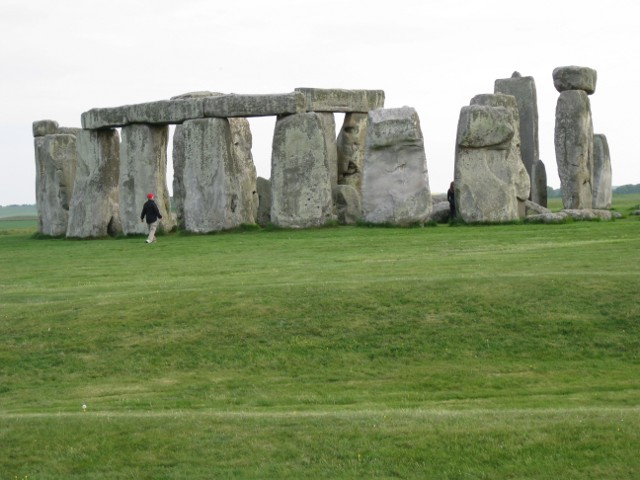
\includegraphics[width=0.95\textwidth]{/part02/Stonehenge.jpg}
  \begin{center}
    {\large ``Stonehenge''}\par
    Foto di radical.librarian\par
    \url{http://www.flickr.com/photos/radical_librarian/3564677324}\par
    Licenza: Attribuzione 2.0 Generico (CC BY 2.0)\par
  \end{center}
\clearpage
\cleardoublepage
 
% (c) 2012 -2014 Dimitrios Vrettos - d.vrettos@gmail.com
\chapter{Insiemi}
\section{Insiemi ed elementi}

In matematica usiamo la parola \textit{insieme} per indicare un
raggruppamento, una collezione, una raccolta di oggetti, individui,
simboli, numeri, figure che sono detti \textit{elementi}
dell'insieme e che sono ben definiti e distinti tra di
loro.

La nozione di insieme e quella di elemento di un insieme in matematica
sono considerate nozioni primitive, nozioni che si preferisce non
definire mediante altre più semplici.

\begin{exrig}
 \begin{esempio}
 Sono insiemi:
 \begin{enumeratea}
  \item l'insieme delle lettere della parola RUOTA;
  \item l'insieme delle canzoni che ho ascoltato la settimana scorsa;
  \item l'insieme delle città della Puglia con più di~$\np{15000}$ abitanti;
  \item l'insieme delle lettere dell'alfabeto italiano;
  \item l'insieme dei numeri~1, 2, 3, 4, 5;
  \item l'insieme delle montagne d'Italia più alte di~$\np{1000}$ metri.
 \end{enumeratea}
 \end{esempio}
\end{exrig}

Per poter assegnare un insieme occorre soddisfare le seguenti condizioni:

\begin{itemize*}
\item bisogna poter stabilire con certezza e oggettività se un oggetto
è o non è un elemento dell'insieme;
\item gli elementi di uno stesso insieme devono essere differenti tra
loro, cioè un elemento non può essere ripetuto più volte nello stesso insieme.
\end{itemize*}

Non possono essere considerati insiemi:
\begin{itemize*}
 \item i film interessanti (non c'è un criterio oggettivo per stabilire se un film è interessante oppure no, uno stesso film
può risultare interessante per alcune persone e non interessante per altre);
 \item le ragazze simpatiche di una classe (non possiamo stabilire in maniera oggettiva se una ragazza è simpatica);
 \item le montagne più alte d'Italia (non possiamo dire se una montagna è tra le più alte poiché non è fissata
un'altezza limite);
 \item l'insieme delle grandi città d'Europa (non c'è un criterio per
stabilire se una città è grande);
\end{itemize*}

\ovalbox{\risolvi \ref{ese:\thechapter.1}}\vspazio


In generale, gli insiemi si indicano con lettere maiuscole~$A$, $B$, $C$, \ldots e
gli elementi con lettere minuscole~$a$, $b$, $c$, \ldots

Se un elemento~$a$ sta nell'insieme~$A$ si scrive~$a\in A$ e si legge ``$a$ appartiene ad~$A$''.
Il simbolo ``$\in$'' si chiama simbolo di \textit{appartenenza}.

Se un elemento~$b$ non sta nell'insieme~$A$ si scrive~$b\notin A$ e
si legge ``$b$ non appartiene ad~$A$''. Il simbolo ``$\notin$''
si chiama simbolo di \textit{non appartenenza}.

Il criterio che stabilisce se un elemento appartiene a un insieme si chiama \textit{proprietà caratteristica} dell'insieme.

Un altro modo per definire un insieme, oltre a quello di indicare la sua proprietà caratteristica, è quello di elencare i suoi elementi separati da virgole e racchiusi tra parentesi graffe. Ad esempio: $A=\{a\text{, }b\text{, }c\text{, }d\}$.

Per indicare alcuni insiemi specifici vengono utilizzati simboli particolari:
\begin{itemize*}
 \item $\insN$ si utilizza per indicare l'insieme dei numeri naturali:~$\insN=\{0\text{, }1\text{, }2\text{, }3\text{, }\ldots\}$;
 \item $\insZ$ si utilizza per indicare i numeri interi relativi:~$\insZ=\{\ldots\text{, }-2\text{, }-1\text{, }0\text{, }+1\text{, }+2\text{, }\ldots\}$;
 \item $\insQ$ si utilizza per indicare i numeri razionali:~$\insQ=\{\dfrac{1}{2}\text{, }-\dfrac{3}{5}\text{, }\dfrac{5}{1}\text{, }-\dfrac{4}{17}\text{, }\np{12,34}\text{, }8\text{, }\np{0,}\overline{25}\text{, }\ldots\}$.
 \end{itemize*}


 \begin{exrig}
 \begin{esempio}
Indica con il simbolo opportuno quali dei seguenti elementi appartengono
o non appartengono all'insieme $A$ dei giorni della
settimana: lunedì, martedì, gennaio, giovedì, dicembre, estate.

Gennaio e dicembre sono mesi dell'anno, perciò scriviamo:
\[\text{lunedì}\in A\text{,~~~}\text{martedì}\in A\text{,~~~}\text{gennaio}\notin A\text{,~~~}\text{giovedì}\in A\text{,~~~}\text{dicembre}\notin A\text{,~~~}\text{estate}\notin A.\]
 \end{esempio}
\end{exrig}

Consideriamo l'insieme~$A=\{\text{r, s, t}\}$ e l'insieme~$B$ delle consonanti della parola
``risate''. Possiamo osservare che~$A$ e~$B$ sono due insiemi costituiti dagli stessi
elementi; diremo che sono \textit{insiemi uguali}.

\begin{definizione}
 Due insiemi~$A$ e~$B$ si dicono \emph{uguali} se sono formati dagli stessi elementi, anche se
disposti in ordine diverso. In simboli si scrive~$A=B$. Altrimenti i due insiemi si dicono \emph{diversi}, in simboli~$A\neq B$.
\end{definizione}

\ovalbox{\risolvii \ref{ese:\thechapter.2}, \ref{ese:\thechapter.3}, \ref{ese:\thechapter.4}, \ref{ese:\thechapter.5}, \ref{ese:\thechapter.6}, \ref{ese:\thechapter.7}, \ref{ese:\thechapter.8}}

\section{Insieme vuoto, insieme universo, cardinalità}\label{sect:universo}

Consideriamo l'insieme~$A=\{\text{consonanti della parola ``AIA''}\}$. Poiché la parola ``AIA'' non
contiene consonanti, l'insieme~$A$ è privo di elementi.

\begin{definizione}
 Un insieme privo di elementi si chiama \emph{insieme vuoto} e lo si indica con il simbolo~$\emptyset$ o $\{ \}$.
\end{definizione}

\osservazione $\{ \}=\emptyset$ ma~$\{\emptyset \}\neq\emptyset$ dato che la scrittura~$\{\emptyset \}$ rappresenta un insieme che ha
come unico elemento l'insieme vuoto.

\begin{exrig}
 \begin{esempio}
 Alcuni insiemi vuoti.
 \begin{enumeratea}
  \spazielenx
\item L'insieme dei numeri negativi maggiori di~5 è vuoto;
\item l'insieme delle capitali europee con meno di~50 abitanti è vuoto;
\item l'insieme dei numeri naturali minori di~0 è vuoto.
 \end{enumeratea}
 \end{esempio}
\end{exrig}

La frase <<l'insieme degli studenti che vengono a scuola con il motorino>> non definisce un
insieme particolare. Occorre definire il contesto, l'ambiente che fa individuare gli elementi
dell'insieme. Se l'ambiente è la classe~1\textsuperscript{a}C gli elementi considerati saranno certamente diversi, e probabilmente meno numerosi, di quelli che compongono l'ambiente di un'intera scuola o di un'intera
città. Quando si identifica un insieme, occorre indicare anche l'ambiente di riferimento da cui trarre gli elementi che appartengono al nostro insieme. Questo insieme si chiama \emph{insieme universo} e rappresenta il contesto, l'ambiente su cui faremo le nostre osservazioni. In generale l'insieme universo per un insieme~$A$ è semplicemente un insieme che contiene~$A$. Solitamente l'insieme universo viene indicato con~$U$.

\subsection{Cardinalità}

\begin{definizione}
 Si definisce \emph{cardinalità} (o \emph{potenza}) di un insieme finito il numero
degli elementi dell'insieme. Essa viene indicata con uno dei seguenti simboli~$\valass{A}$, \#($A$) o~$\card(A)$.
\end{definizione}

Per poter parlare di cardinalità di un insieme qualsiasi, che
comprenda anche insiemi infiniti come gli insiemi numerici, occorre una
definizione più complessa che qui non daremo.

\begin{exrig}
 \begin{esempio}
 Esempi di cardinalità.
 \begin{enumeratea}
  \item L'insieme~$A$ delle vocali dell'alfabeto italiano ha~5 elementi, quindi~$\card(A)=5$;
  \item l'insieme~$B$ dei multipli di~3 minori di~10 ha~3 elementi, quindi~$\card(B)=3$.
 \end{enumeratea}
 \end{esempio}
\end{exrig}

\ovalbox{\risolvii \ref{ese:\thechapter.9}, \ref{ese:\thechapter.10}, \ref{ese:\thechapter.11}, \ref{ese:\thechapter.12}, \ref{ese:\thechapter.13}, \ref{ese:\thechapter.14}}

\section{Rappresentazione degli insiemi}

Esistono diversi modi per rappresentare un insieme e quindi per indicare
con precisione i suoi elementi.

\subsection{Rappresentazione tabulare}

La rappresentazione tabulare è la descrizione più elementare di un
insieme; consiste nell'elencare tutti gli elementi dell'insieme separati da virgole e racchiusi tra le
parentesi graffe.

Per esempio, definiamo un insieme~$X$ con la scrittura:~$X=\{\text{1, 2, 3, 5}\}$.
Non è importante l'ordine in cui vengono scritti gli elementi, cioè
\[X=\{\text{1, 2, 3, 5}\}=\{\text{2, 1, 5, 3}\}.\]

È invece necessario che ogni elemento dell'insieme compaia una sola volta. Ad esempio, per rappresentare
l'insieme~$Y$ delle lettere della parola ``autunno'', scriviamo
\[Y = \{\text{a, u, t, n, o}\}.\]

Si può utilizzare questa rappresentazione anche per insiemi numerosi e addirittura infiniti. In questi casi si elencano i primi elementi
dell'insieme e in fondo all'elenco si mettono tre punti di sospensione lasciando intendere come continuare la serie.

Per esempio, l'insieme dei multipli di~3 si può indicare con la seguente rappresentazione tabulare:
\[X=\{\text{0, 3, 6, 9, 12, 15, 18, 21, }\ldots\}.\]


\begin{exrig}
 \begin{esempio}
Rappresentazione degli insiemi:
 \begin{enumeratea}
\item l'insieme~$G$ dei primi~3 giorni della settimana si indica:~$G=\{\text{lunedì, martedì, mercoledì}\}$;
\item l'insieme~$A$ delle lettere della parola ``associazione'' si indica:~$A=\{\text{a, s, o, c, i, z, n, e}\}$.
\end{enumeratea}
 \end{esempio}
\end{exrig}

\ovalbox{\risolvii \ref{ese:\thechapter.15}, \ref{ese:\thechapter.16}, \ref{ese:\thechapter.17}, \ref{ese:\thechapter.18}}

\subsection{Rappresentazione per proprietà caratteristica}

Per quegli insiemi i cui elementi soddisfano una certa proprietà che
li caratterizza, possiamo usare proprio questa proprietà per
descrivere più sinteticamente l'insieme che li contiene.

Per esempio, l'insieme~$Y$ dei divisori di~10 può essere definito come: \[Y=\{x\mid x \text{ è un divisore di }10\}\]
e si legge ``$Y$ è l'insieme degli elementi~$x$ tali che~$x$ è un divisore di~10''.

In questa scrittura si mette in evidenza la caratteristica degli elementi dell'insieme.
La rappresentazione tabulare dello stesso insieme è~$Y=\{\text{1, 2, 5, 10}\}$. L'espressione ``tale che'', che è stata rappresentata per mezzo del simbolo ``$|$'', può essere indicata anche per mezzo del simbolo ``:''.

La rappresentazione per caratteristica dell'insieme~$X$
dei naturali minori di~15 è: \[X=\{x\in\insN\mid x<15\}\]
e si legge ``$X$ è l'insieme dei numeri naturali~$x$ tali che~$x$ è minore di~15''.

L'insieme che viene indicato nella prima parte della rappresentazione (nell'ultimo esempio è
l'insieme dei numeri naturali~$\insN$) è l'\textit{insieme universo} (sezione \ref{sect:universo}) al quale si fa riferimento.
Questo metodo è particolarmente utile quando l'insieme da rappresentare contiene molti elementi.

\begin{exrig}
 \begin{esempio}
 Esempi di definizioni di insiemi per mezzo della loro proprietà caratteristica:
 \begin{enumeratea}
\item l'insieme~$A$ delle rette incidenti a una retta~$t$ assegnata si può rappresentare come:
\[A=\{r\mid r\text{ è una retta incidente a } t\}\]
\item l'insieme~$B$ dei numeri naturali maggiori di~100 può essere rappresentato come:
\[B=\{n\in\insN\mid n>100\}\]
\item l'insieme~$P$ dei numeri pari può essere rappresentato come:
\[P=\{n\in\insN\mid n=2\cdot m\text{, con }m\in\insN\}\]
\item l'insieme~$C$ dei numeri interi relativi compresi tra~$-10$ e~$+100$, estremi inclusi:
\[C=\{n\in\insZ\mid -10\le n\le 100\}.\]
\end{enumeratea}
 \end{esempio}
\end{exrig}

\ovalbox{\risolvii \ref{ese:\thechapter.19}, \ref{ese:\thechapter.20}, \ref{ese:\thechapter.21}, \ref{ese:\thechapter.22}, \ref{ese:\thechapter.23}, \ref{ese:\thechapter.24}, \ref{ese:\thechapter.25}, \ref{ese:\thechapter.26}, \ref{ese:\thechapter.27}, \ref{ese:\thechapter.28}, \ref{ese:\thechapter.29},%
\ref{ese:\thechapter.30}, \ref{ese:\thechapter.31}, \ref{ese:\thechapter.32}}

\subsection{Rappresentazione grafica (Diagramma di Eulero-Venn)}

In questa rappresentazione grafica, detta anche \textit{rappresentazione
di Eulero-Venn}\footnote{in onore del matematico svizzero Leonhard Euler, noto in Italia come Eulero, (1707 - 1783) e del matematico e statistico inglese John Venn (1834 - 1923).} si disegna una linea chiusa all'interno della quale gli elementi
dell'insieme si indicano con dei punti. Solitamente si scrive all'esterno il nome dell'insieme
e vicino ad ogni punto il valore ad esso associato.

\begin{exrig}
 \begin{esempio}
 $A$ è l'insieme dei numeri naturali minori di~6, cioè $A=\{\text{0, 1, 2, 3, 4, 5}\}$.
 La sua rappresentazione con un diagramma di Eulero-Venn è la seguente
 \begin{center}
  % (c) 2012 Dimitrios Vrettos - d.vrettos@gmail.com
\begin{tikzpicture}[x=2cm,font=\small]
\draw (0,0)circle (1) (0,1) node[ left=1] {$A$};
\begin{scope}[fill=CornflowerBlue, draw=black]
\foreach \x/\xtext in {-.5/0,0/1,.5/2}
\filldraw (\x,.2) circle (2pt) node[above right] {\xtext};
\foreach \y/\ytext in {-.5/3,0/4,.5/5}{
\filldraw (\y,-.7) circle (2pt) node[above right] {\ytext};
}
\end{scope}
\end{tikzpicture}

 \end{center}

 \end{esempio}

 \begin{esempio}
 $B$ è l'insieme delle lettere della parola ``TARTARUGA'', $B=\{\text{t, a, r, u, g}\}$.
 La sua rappresentazione con un diagramma di Eulero-Venn è la seguente
 \begin{center}
  % (c) 2012 Dimitrios Vrettos - d.vrettos@gmail.com
\begin{tikzpicture}[x=2cm,font=\small]
\draw (0,0)circle (1) (0,1) node[ left=1] {$B$};
\begin{scope}[fill=CornflowerBlue, draw=black]
\foreach \x/\xtext in {-.5/t,0/a,.5/r}
\filldraw (\x,.2) circle (2pt) node[above right] {\xtext};
\foreach \y/\ytext in {-.25/u,.25/g}{
\filldraw (\y,-.7) circle (2pt) node[above right] {\ytext};
}
\end{scope}
\end{tikzpicture}

 \end{center}

 \end{esempio}

\end{exrig}

Un insieme può essere rappresentato con una qualsiasi delle
rappresentazioni indicate. Se un insieme è infinito o è costituito
da un numero elevato di elementi la rappresentazione più pratica è
quella per caratteristica.

\begin{exrig}
 \begin{esempio}
 Rappresentare l'insieme~$C$ dei multipli di~5.

 Per caratteristica:~$C=\{n\in\insN\mid n\text{ è multiplo di }5\}$ oppure
$C=\{n\in\insN\mid n=5\cdot m$, $m\in\insN\}$

Tabulare:~$C=\{\text{0, 5, 10, 15, 20, 25, 30, 35, }\dots\}$. I puntini di sospensione indicano che l'elenco continua.

Rappresentazione con diagramma di Eulero-Venn:
\begin{center}
 % (c) 2012 Dimitrios Vrettos - d.vrettos@gmail.com
\begin{tikzpicture}[x=1.5cm,font=\small]
    \draw (0,0)circle (1.5) (0,1) node[ left=1.5] {$C$};
    \begin{scope}[fill=CornflowerBlue, draw=black]
\foreach \x/\xtext in {-.6/5,0/10,.6/15}
\filldraw (\x,.7) circle (2pt) node[above right] {\xtext};
\foreach \y/\ytext in {-.6/20,0/25,.6/30}
\filldraw (\y,0) circle (2pt) node[above right] {\ytext};
\foreach \z/\ztext in {-.6/30,0/35,.6/{}}
\filldraw(\z,-.7) circle (2pt) node [above right]  {\ztext};
\end{scope}
\end{tikzpicture}

\end{center}
 \end{esempio}
\end{exrig}

\ovalbox{\risolvii \ref{ese:\thechapter.33}, \ref{ese:\thechapter.34}, \ref{ese:\thechapter.35}, \ref{ese:\thechapter.36}, \ref{ese:\thechapter.37}, \ref{ese:\thechapter.38}, \ref{ese:\thechapter.39}, \ref{ese:\thechapter.40}}

\section{Sottoinsieme}

Consideriamo l'insieme~$A$ degli abitanti di Milano e l'insieme~$B$ degli abitanti di Milano
con età superiore ai~40 anni. Gli abitanti ultra quarantenni di Milano fanno parte della popolazione di Milano, cioè tutti gli
elementi dell'insieme~$B$ sono anche elementi di~$A$: si dice che~$B$ è sottoinsieme di~$A$ e si scrive~$B\subseteq A$.

\begin{definizione}
Dati due insiemi~$X$ e~$Y$, si dice che~$Y$ è un \emph{sottoinsieme} di~$X$
se ogni elemento di~$Y$ è anche elemento di~$X$.
In simboli:~$Y\subseteq X$, che si legge
``$Y$ è incluso in~$X$'' o ``$Y$ è sottoinsieme di~$X$''.
\end{definizione}

La rappresentazione con un diagramma di Eulero-Venn è la seguente:
\begin{center}
% (c) 2012 Dimitrios Vrettos - d.vrettos@gmail.com
\begin{tikzpicture}[x=2cm,font=\small, fill=CornflowerBlue]
    \draw (0,0)circle (1.5) (0,1) node[ left=1.5] {$X$};
\foreach \x in {-.5,0,.5}
\foreach \y in {-.5,0,.5}
\filldraw (\x,\y) circle (2pt) node[above right] {};
\begin{scope}[y=2cm]]
    \draw (0.25,0)circle (.5) (0,.5) node[left=.1] {$Y$};
\end{scope}
\end{tikzpicture}

\end{center}
Se~$a$ è un elemento del sottoinsieme~$Y$, allora lo sarà anche dell'insieme~$X$:
\begin{center}
se~$a\in Y$ e~$Y\subseteq X$, allora~$a\in X$\qquad oppure \qquad $a\in Y$ e~$Y\subseteq X \:\Rightarrow\:a\in X$.
\end{center}

Dalla stessa definizione, si deduce che ogni insieme è sottoinsieme di
se stesso, in simboli~$X\subseteq X$.

Nel caso in cui tutti gli elementi di~$Y$ siano elementi di~$X$ e tutti gli elementi di~$X$ siano elementi di
$Y$ si ha che~$X=Y$, e~$Y$ si dice \emph{sottoinsieme improprio} di~$X$.
Se~$X\subseteq Y$ e~$Y\subseteq X$, allora~$Y=X$.

Tra i sottoinsiemi di un insieme si considera anche
l'insieme vuoto. Cioè, qualunque sia
l'insieme~$X$ risulta~$\emptyset \subseteq X$.
Quindi l'insieme vuoto è considerato un sottoinsieme improprio di qualunque insieme.

Se~$Y$ è un sottoinsieme non vuoto di~$X$ e~$X$ ha altri elementi oltre a quelli di~$Y$
si dice che~$Y$ è un \emph{sottoinsieme proprio} di~$X$ e si scrive~$Y\subset X$.

La scrittura~$Y\subseteq X$ si usa quando non si sa in modo certo se~$Y=X$ o meno.

\begin{exrig}

\begin{esempio}
Consideriamo l'insieme~$X=\{$lettere della parola ``autunno''$\}$ e
l'insieme~$Y=\{$lettere della parola ``notaio''$\}$; possiamo affermare che ogni
elemento di~$Y$ è anche elemento di~$X$? La risposta è negativa, infatti~$\text{i}\in Y$ ma
$\text{i}\notin X$ quindi~$Y$ non è sottoinsieme di~$X$ e si scrive~$Y\not\subset X$.
\end{esempio}

\begin{esempio}
Sia~$A$ l'insieme delle lettere dell'alfabeto italiano e~$V$
l'insieme delle vocali, allora si può scrivere
$V\subset A$; cioè~$V$ è un sottoinsieme proprio di~$A$,
come si può anche vedere dalla rappresentazione grafica.
\begin{center}
 % (c) 2012 Dimitrios Vrettos - d.vrettos@gmail.com
\begin{tikzpicture}[x=2cm,font=\footnotesize, fill=CornflowerBlue]
    \draw (0,0)circle (1.5) (0,1) node[ left=1.5] {$A$};
\filldraw (-.8,.6) circle (1pt) node[above right] {a};
\filldraw (-1.1,.4) circle (1pt) node[above right] {e};
\filldraw (-.6,-.15) circle (1pt) node[above right] {i};
\filldraw (-.8,.2) circle (1pt) node[above right] {o};
\filldraw (-1.1,0) circle (1pt) node[above right] {u};

\filldraw (-.1,1.1) circle (1pt) node[above right] {b};
\filldraw (-.1,.7) circle (1pt) node[above right] {c};
\filldraw (.1,.8) circle (1pt) node[above right] {d};
\filldraw (.5,0) circle (1pt) node[above right] {f};
\filldraw (.65,-.8) circle (1pt) node[above right] {g};
\filldraw (-1.2,-.7) circle (1pt) node[above right] {h};
\filldraw (1.1,0) circle (1pt) node[above right] {l};
\filldraw (1,-.5) circle (1pt) node[above right] {m};
\filldraw (-.3,-.2) circle (1pt) node[above right] {n};
\filldraw (-.5,-.9) circle (1pt) node[above right] {p};
\filldraw (.8,.3) circle (1pt) node[above right] {q};
\filldraw (.6,.7) circle (1pt) node[above right] {r};
\filldraw (.2,-.4) circle (1pt) node[above right] {s};
\filldraw (.2,.3) circle (1pt) node[above right] {t};
\filldraw (-.1,-.8) circle (1pt) node[above right] {v};
\filldraw (.3,-.9) circle (1pt) node[above right] {z};
 \begin{scope}[y=2cm]]
     \draw (-.8,.15)circle (.4) (0,.6) node[left=.4] {$V$};
 \end{scope}
\end{tikzpicture}

\end{center}
\end{esempio}

\begin{esempio}
Sia~$C=\{1\}$, allora~$C$ non ha sottoinsiemi propri;
mentre i suoi sottoinsiemi impropri sono~$C=\{1\}$ e
l'insieme vuoto~$\emptyset $.
\end{esempio}

\begin{esempio}
Sia~$A$ l'insieme delle auto esposte in un
autosalone e~$U$ l'insieme delle auto usate
esposte nello stesso autosalone. Si ha che~$U$ è un
sottoinsieme di~$A$, ma senza avere ulteriori informazioni non
possiamo escludere che tutte le auto esposte siano usate, dobbiamo
perciò scrivere~$U\subseteq A$. Se invece sappiamo che nessuna
auto esposta è usata, allora~$U=\emptyset $.
\end{esempio}
\end{exrig}

\ovalbox{\risolvii \ref{ese:\thechapter.41}, \ref{ese:\thechapter.42}, \ref{ese:\thechapter.43}, \ref{ese:\thechapter.44}, \ref{ese:\thechapter.45}, \ref{ese:\thechapter.46}}

\section{Insieme delle parti}

Consideriamo l'insieme~$A$ dei numeri naturali
compresi tra~0 e~100. A partire da questo insieme possiamo formare
gruppi costituiti dai soli numeri multipli di~10, dai numeri pari, da
quelli dispari, da quelli divisibili per~7 e così via. Quindi con gli
elementi dell'insieme~$A$ possiamo formare molti
altri insiemi che sono sottoinsiemi di~$A$.

\begin{exrig}
 \begin{esempio}
Determinare tutti i sottoinsiemi di~$A=\{$1, 2, 3$\}$.

$\emptyset \subseteq A$, infatti l'insieme vuoto è un
sottoinsieme improprio di qualunque insieme.

Elenchiamo tutti i sottoinsiemi costituiti da un solo elemento: $\{1\}$, $\{2\}$, $\{3\}$.
Elenchiamo ora tutti i sottoinsiemi costituiti da due elementi: $\{$1, 2$\}$, $\{$1, 3$\}$, $\{$2, 3$\}$.
L'unico sottoinsieme costituito da tre elementi è~$A$ stesso, possiamo scrivere:
$\{$1, 2, 3$\}\subseteq A$. In tutto si hanno 8 sottoinsiemi.
 \end{esempio}

\end{exrig}

\begin{definizione}
Dato un insieme~$A$, si chiama \emph{insieme delle parti} o (\emph{insieme potenza}) di~$A$ l'insieme $\wp(A)$ che ha come elementi
tutti i sottoinsiemi propri ed impropri di~$A$.
\end{definizione}

L'insieme delle parti di un insieme $A$ ha sempre come
elementi~$\emptyset $ e~$A$, quindi~$\emptyset\in\wp (A)$ e
$A\in\wp (A)$.
Il numero degli elementi di~$\wp (A)$, cioè dei suoi possibili
sottoinsiemi, propri e impropri, dipende dal numero degli elementi di~$A$.

\begin{exrig}
 \begin{esempio}
 L'insieme vuoto ha come unico sottoinsieme se stesso,
quindi~$\wp (\emptyset )=\{\emptyset \}$.
 \end{esempio}

\begin{esempio}
 Dato l'insieme~$A=\{a\}$, i suoi possibili sottoinsiemi
propri ed impropri sono:~$S_{1}=\emptyset$, $S_{2}=\{a\}$;
allora~$\wp (A)=\{S_{1}\text{, }S_{2}\}$.
 \end{esempio}

\begin{esempio}
 Dato l'insieme~$B=\{\text{matita, penna}\}$ i
suoi possibili sottoinsiemi propri ed impropri sono:~$S_{1}=\emptyset$,
$S_{2}=B=\{\text{matita, penna}\}$, $S_{3}=\{\text{matita}\}$,
$S_{4}=\{\text{penna}\}$;
allora~$\wp (A)=\{S_{1}\text{, }S_{2}\text{, }S_{3}\text{, }S_{4}\}$.
 \end{esempio}

\begin{esempio}
 Dato l'insieme~$B=\{\text{1, 2, 3}\}$, i suoi possibili
sottoinsiemi propri ed impropri sono:~$S_{1}=\emptyset$,
$S_{2}=B=\{\text{1, 2, 3}\}$, $S_{3}=\{1\}$, $S_{4}=\{2\}$, $S_{5}=\{3\}$,
$S_{6}=\{1\text{, }2\}$, $S_{7}=\{1\text{, }3\}$, $S_{8}=\{2\text{, }3\}$;
allora~$\wp (A)=\{S_{1}\text{, }S_{2}\text{, }S_{3}\text{, }S_{4}\text{, }S_{5}\text{, }S_{6}\text{, }S_{7}\text{, }S_{8}\}$.
 \end{esempio}
 \end{exrig}

 Riassumendo:
\begin{itemize*}
\item se~$A=\emptyset $ l'insieme delle parti ha~1 solo elemento;
\item se~$A$ ha~1 elemento allora l'insieme delle parti ha~2 elementi;
\item se~$A$ ha~2 elementi, l'insieme delle parti ne ha~4;
\item se~$A$ ha~3 elementi, l'insieme delle parti ne ha~8.
\end{itemize*}

Generalizzando, se~$A$ ha~$n$ elementi, l'insieme delle parti $\wp (A)$ ne ha~$2^{n}$.

\vspazio\ovalbox{\risolvii \ref{ese:\thechapter.47}, \ref{ese:\thechapter.48}, \ref{ese:\thechapter.49}, \ref{ese:\thechapter.50}, \ref{ese:\thechapter.51}}

\section{Insieme unione}

Prendiamo l'insieme~$P$ dei numeri pari e l'insieme~$D$ dei numeri dispari; allora
l'insieme~$\insN$ dei numeri naturali è dato dall'unione dei due insiemi~$P$ e~$D$.

\begin{definizione}
Dati due insiemi~$A$ e~$B$, si dice
\emph{insieme unione} l'insieme~$C$, composto da tutti gli elementi appartenenti ad
$A$ o a~$B$ o a entrambi.
In simboli:~$C=A\cup B$ e si legge ``$A$ unito a~$B$''
o ``$A$ unione~$B$''.
\end{definizione}
\begin{center}
 % (c) 2012 Dimitrios Vrettos - d.vrettos@gmail.com
\begin{tikzpicture}[filled/.style={fill=circle area, draw=black, thin}]

\def\firstcircle{(0,0) circle (1.5cm)}
\def\secondcircle{(0:2cm) circle (1.5cm)}

\definecolor{circle area}{gray}{.9}

 \draw[filled] \firstcircle node {$A$}
                  \secondcircle node {$B$};
 \node[anchor=south] at (current bounding box.north) {$A \cup B$};
\end{tikzpicture}

\end{center}
Mediante la proprietà caratteristica si scrive:~$C=A\cup B=\{x\mid (x\in A)\text{ o }(x\in B)\}$.

\subsection{Proprietà dell'unione tra insiemi}

\begin{enumeratea}
\item $A\cup B=B\cup A$: proprietà \emph{commutativa} dell'unione;
\item $(A\cup B)\cup C=A\cup (B\cup C)$: proprietà \emph{associativa} dell'unione;
\item se~$B\subset A$, allora~$A\cup B=A$;
\item $A\cup \emptyset =A$;
\item $A\cup A=A$: proprietà di \emph{idempotenza} dell'unione;
\item $\emptyset \cup \emptyset = \emptyset $.
\end{enumeratea}
\pagebreak
\begin{exrig}
 \begin{esempio}
Siano~$D=\{$1, 3, 5$\}$ e~$P=\{$2, 4, 6$\}$ allora~$N=P\cup D=\{$1, 2, 3, 4, 5, 6$\}$.
\begin{center}
 % (c) 2012 Dimitrios Vrettos - d.vrettos@gmail.com
\begin{tikzpicture}[font=\small, fill=CornflowerBlue]
\draw (0,1.25)circle (1) (-1,2.25) node[above] {$D$};
\draw(0,-1.25) circle (1) (-1,-.5) node [above]  {$P$};
\draw (3.5,0) circle (1.5) (3.5,1.5) node [above]  {$N$};

\filldraw (-.5,1.1) circle (2pt) node[above right] {1};
\filldraw (0,1.6) circle (2pt) node[above right] {3};
\filldraw (.4,.9) circle (2pt) node[above right] {5};

\filldraw (-.5,-1.5) circle (2pt) node[above right] {6};
\filldraw (0,-1) circle (2pt) node[above right] {4};
\filldraw (.4,-1.9) circle (2pt) node[above right] {2};

\filldraw (2.5,.5) circle (2pt) node[above right] {1};
\filldraw (3.5,1) circle (2pt) node[above right] {3};
\filldraw (4,-.8) circle (2pt) node[above right] {5};

\filldraw (3,-1) circle (2pt) node[above right] {6};
\filldraw (2.5,-.7) circle (2pt) node[above right] {4};
\filldraw (3.4,0) circle (2pt) node[above right] {2};

\node (d) at (1,1.25) {};
\node (p) at (1,-1.25) {};
\node (n) at (2,0) {};

\begin{scope}[blue, ->,thick]
\draw (d)--(n.north);
\draw (p)--(n.south);
\end{scope}
\end{tikzpicture}

\end{center}

\end{esempio}

\begin{esempio}
Siano~$X=\{$do, re, mi, fa, sol, la, si$\}$
e~$Y=\{$do, re, mi$\}$, allora, poiché $Y\subset X$, $W=X\cup Y=X=\{$do, re, mi, fa, sol, la, si$\}$.
\begin{center}
 % (c) 2012 Dimitrios Vrettos - d.vrettos@gmail.com
\begin{tikzpicture}[fill=CornflowerBlue]
\begin{scope}[font=\small]
\draw (0,1.25)circle (1) (-1,2.25) node[above] {$X$};
\draw(0,-1.25) circle (1) (-1,-.5) node [above]  {$Y$};
\draw (3.5,0) circle (1.5) (3.5,1.5) node [above]  {$W=X$};
\draw(3,-.4) circle (.75) (2.4,0) node [above] {$Y$};
\end{scope}
\begin{scope}[font=\scriptsize]
\filldraw (-.5,1.1) circle (1pt) node[above right] {do};
\filldraw (0,1.6) circle (1pt) node[above right] {re};
\filldraw (.4,.9) circle (1pt) node[above right] {mi};
\filldraw (0,1) circle (1pt) node[above right] {fa};
\filldraw (-.6,1.6) circle (1pt) node[above right] {sol};
\filldraw (0,.4) circle (1pt) node[above right] {la};
\filldraw (-.4,.6) circle (1pt) node[above right] {si};

\filldraw (-.5,-1.5) circle (1pt) node[above right] {do};
\filldraw (0,-1) circle (1pt) node[above right] {mi};
\filldraw (.4,-1.9) circle (1pt) node[above right] {re};

\filldraw (2.5,-.6) circle (1pt) node[above right] {do};
\filldraw (2.9,-.7) circle (1pt) node[above right] {re};
\filldraw (2.9,-.1) circle (1pt) node[above right] {mi};
\filldraw (3,1) circle (1pt) node[above right] {fa};
\filldraw (3.2,.5) circle (1pt) node[above right] {sol};
\filldraw (3.9,.4) circle (1pt) node[above right] {la};
\filldraw (4,-.6) circle (1pt) node[above right] {si};
\end{scope}
\node (x) at (1,1.25) {};
\node (y) at (1,-1.25) {};
\node (w) at (2,0) {};

\begin{scope}[red, ->,thick]
\draw (x)--(w.north);
\draw (y)--(w.south);
\end{scope}
\end{tikzpicture}

\end{center}

\end{esempio}
\end{exrig}

\ovalbox{\risolvii \ref{ese:\thechapter.52}, \ref{ese:\thechapter.53}, \ref{ese:\thechapter.54}, \ref{ese:\thechapter.55}}

\section{Insieme intersezione}

\begin{exrig}
\vspace{1.05ex}
 \begin{esempio}
Se~$A$ è l'insieme delle lettere della parola ``matematica'' e~$B$ è l'insieme delle lettere della parola
``materia''. Quali elementi di~$A$ stanno in~$B$? Quali elementi di~$B$ stanno in~$A$? Quali sono gli elementi
che stanno in entrambi gli insiemi?

\begin{itemize*}
 \item L'insieme degli elementi di~$A$ che stanno in~$B$ è $\{$m, a, t, e, i$\}$;
 \item l'insieme degli elementi di~$B$ che stanno in~$A$ è $\{$m, a, t, e, i$\}$;
 \item l'insieme degli elementi che stanno sia in~$A$ sia in~$B$ è $\{$m, a, t, e, i$\}$.
\end{itemize*}
\end{esempio}
\end{exrig}

\begin{definizione}
Dati due insiemi~$A$ e~$B$, si dice \emph{insieme intersezione} di~$A$ e~$B$, l'insieme
$C$ composto da tutti gli elementi appartenenti contemporaneamente ad
$A$ e a~$B$, ossia comuni a entrambi.
In simboli:~$C=A\cap B$, che si legge
``$A$ intersecato a~$B$'' o ``$A$ intersezione~$B$''.
\end{definizione}
\begin{center}
 % (c) 2012 Dimitrios Vrettos - d.vrettos@gmail.com
\begin{tikzpicture}[filled/.style={fill=circle area, draw=circle edge, thick}]
\def\firstcircle{(0,0) circle (1.5cm)}
\def\secondcircle{(0:2cm) circle (1.5cm)}

\definecolor{circle edge}{gray}{0.9}
\definecolor{circle area}{gray}{0.9}
    \begin{scope}
        \clip \firstcircle;
        \fill[filled] \secondcircle;
    \end{scope}
    \draw\firstcircle node {$A$};
    \draw \secondcircle node {$B$};
    \node[anchor=south] at (current bounding box.north) {$A \cap B$};
\end{tikzpicture}

\end{center}
Mediante proprietà caratteristica si scrive:~$C=A\cap B=\{x\mid (x\in A)\text{ e }(x\in B)\}$.

\subsection{Proprietà dell'intersezione tra insiemi}

\begin{enumeratea}
\item $A\cap B=B\cap A$: proprietà \emph{commutativa} dell'intersezione;
\item $(A\cap B)\cap C=A\cap (B\cap C)$: proprietà \emph{associativa} dell'intersezione;
\item Se~$B\subset A$, allora~$A\cap B=B$;
\item $A\cap \emptyset =\emptyset$;
\item $A\cap A=A$: proprietà di \emph{idempotenza} dell'intersezione;
\item $\emptyset \cap \emptyset =\emptyset$.
\end{enumeratea}

\subsection[Proprietà distributiva dell'intersezione]{Proprietà distributiva dell'intersezione rispetto all'unione e viceversa}

\begin{enumeratea}
\item $A\cap (B\cup C)=(A\cap B)\cup (A\cap C)$: proprietà \emph{distributiva dell'intersezione rispetto all'unione};
\item $A\cup (B\cap C)=(A\cup B)\cap (A\cup C)$: proprietà \emph{distributiva dell'unione rispetto all'intersezione}.
\end{enumeratea}

\begin{definizione}
Dati due insiemi~$A$ e~$B$, essi si dicono \emph{disgiunti} se non hanno elementi in comune, ossia se la loro intersezione è vuota. In simboli~$A \cap B = \emptyset$.
\end{definizione}

\begin{exrig}
 \begin{esempio}
Siano~$X=\{\text{do, re, mi. fa, sol, la, si}\}$
e~$Y=\{\text{do, re, mi}\}$. Allora poiché, 
$Y\subset X$, si ha:~$W=X\cap Y=Y=\{\text{do, re, mi}\}$.
 \end{esempio}

 \begin{esempio}
Siano~$D=\{\text{1, 3, 5}\}$ e~$P=\{\text{2, 4, 6}\}$ allora~$N=P\cap D=\emptyset$.
\begin{center}
 % (c) 2012 Dimitrios Vrettos - d.vrettos@gmail.com
\begin{tikzpicture}[font=\small, fill=CornflowerBlue]
\draw (0,1.25)circle (1) (-1,2.25) node[above] {$D$};
\draw(0,-1.25) circle (1) (-1,-.5) node [above]  {$P$};
\draw (3.5,0) circle (1) (3.5,1) node [above]  {$D$};
\draw (5,0) circle (1) (5,1) node [above]  {$P$};

\filldraw (-.5,1.1) circle (1pt) node[above right] {1};
\filldraw (0,1.6) circle (1pt) node[above right] {3};
\filldraw (.4,.9) circle (1pt) node[above right] {5};

\filldraw (-.5,-1.5) circle (1pt) node[above right] {0};
\filldraw (0,-1) circle (1pt) node[above right] {4};
\filldraw (.4,-1.9) circle (1pt) node[above right] {2};

\filldraw (3.5,.5) circle (1pt) node[above right] {1};
\filldraw (3,0) circle (1pt) node[above right] {3};
\filldraw (3.5,-.5) circle (1pt) node[above right] {5};

\filldraw (5,-.5) circle (1pt) node[above right] {0};
\filldraw (5,0) circle (1pt) node[above right] {4};
\filldraw (4.8,.5) circle (1pt) node[above right] {2};

\node (d) at (1,1.25) {};
\node (p) at (1,-1.25) {};
\node (n) at (2.5,0) {};

\begin{scope}[blue, ->,thick]
\draw (d)--(n.north);
\draw (p)--(n.south);
\end{scope}
\end{tikzpicture}

\end{center}
 \end{esempio}
\end{exrig}

\ovalbox{\risolvii \ref{ese:\thechapter.56}, \ref{ese:\thechapter.57}, \ref{ese:\thechapter.58}, \ref{ese:\thechapter.59}}

\subsection{Insieme differenza}

Consideriamo gli insiemi~$A$ e~$B$ formati rispettivamente
dalle lettere dell'alfabeto italiano e dalle
consonanti dell'alfabeto italiano cioè:
$A=\{$a, b, c, d, e, f, g, h, i, l, m, n, o, p, q, r, s, t, u, v, z$\}$ e
$B=\{$b, c, d, f, g, h, l, m, n, p, q, r, s, t, v, z$\}$, le lettere ``a, e, i, o, u'' che compaiono
nell'insieme~$A$ ma non in~$B$ formano un nuovo insieme chiamato insieme \emph{differenza} tra $A$ e $B$.

\begin{definizione}
 Dati due insiemi~$A$ e~$B$, si dice \emph{insieme differenza} tra $A$ e $B$ l'insieme~$C$ composto da tutti gli elementi
di~$A$ che non appartengono a~$B$. In simboli:~$C=A-B$ o anche $C=A \backslash B$.
\end{definizione}

\begin{center}
% (c) 2012 Dimitrios Vrettos - d.vrettos@gmail.com
\begin{tikzpicture}[filled/.style={fill=circle area, draw=circle edge, thick}]
\def\firstcircle{(0,0) circle (1.5cm)}
\def\secondcircle{(0:2cm) circle (1.5cm)}

\definecolor{circle edge}{gray}{0.9}
\definecolor{circle area}{gray}{0.9}
\begin{scope}
\clip \firstcircle;
\draw[filled, even odd rule] \firstcircle node {$A$}
\secondcircle;
\end{scope}
\draw\firstcircle;
\draw \secondcircle node {$B$};
\node[anchor=south] at (current bounding box.north) {$A- B$};
\end{tikzpicture}

\end{center}
Mediante proprietà caratteristica si scrive:~$C=A-B=\{x\mid (x\in A)\text{ e }(x\notin B)\}$.

\subsection{Proprietà della differenza tra insiemi}

\begin{enumeratea}
\item $A-A=\emptyset$;
\item $A-\emptyset =A$;
\item se~$A\cap B=\emptyset $, ossia $A$ e $B$ sono disgiunti, allora~$A-B=A$, e~$B-A=B$;
\item se~$B\subset A$, ossia~$B$ è sottoinsieme proprio di~$A$, allora~$B-A=\emptyset $.
\end{enumeratea}

\begin{exrig}
 \begin{esempio}
Siano~$A=\{$ 8, 9, 10, 12, 13$\}$ e~$B=\{$9, 10, 11, 13$\}$, allora
$C=A-B=\{$8, 12$\}$ e~$D=B-A=\{11\}$.
 \end{esempio}
\end{exrig}

Poiché in genere $A-B\neq B-A$, nella differenza tra insiemi non vale la proprietà
commutativa.

\begin{exrig}
 \begin{esempio}
Siano~$D=\{$1, 3, 5$\}$ e~$P=\{$0, 2, 4$\}$. I due insiemi sono disgiunti poiché ~$P\cap D=\emptyset$,
 quindi~$D-P=\{$1, 3, 5$\}=D$ e~$P-D=\{$0, 2, 4$\}=P$.
\begin{center}
 % (c) 2012 Dimitrios Vrettos - d.vrettos@gmail.com
\begin{tikzpicture}[font=\small]
\draw (0,1.25)circle (1) (-1,2.25) node[above] {$A$};
\draw(0,-1.25) circle (1) (-1,-.5) node [above]  {$B$};
\draw (3.5,0) circle (1.5) (3.5,1.5) node [above]  {$A$};
\draw (5,0) circle (1.5) (5,1.5) node [above]  {$B$};

\fill (-.5,1.1) circle (1pt) node[above right] {8};
\fill (0,1.6) circle (1pt) node[above right] {9};
\fill (.4,1.1) circle (1pt) node[above right] {12};
\fill (-.4,.7) circle (1pt) node[above right] {13};
\fill (.1,.4) circle (1pt) node[above right] {10};

\fill (-.5,-1.5) circle (1pt) node[above right] {10};
\fill (0,-1) circle (1pt) node[above right] {9};
\fill (.3,-1.9) circle (1pt) node[above right] {11};
\fill (-.3,-1.9) circle (1pt) node[above right] {13};

\fill (4,.5) circle (1pt) node[above right] {13};
\fill (3,0) circle (1pt) node[above right] {8};
\fill (2.8,-.8) circle (1pt) node[above right] {12};

\fill (4,-.75) circle (1pt) node[above right] {10};
\fill (4.25,0) circle (1pt) node[above right] {9};
\fill (5.5,0) circle (1pt) node[above right] {11};

\node (a) at (1,1.25) {};
\node (b) at (1,-1.25) {};
\node (n) at (2,0) {};

\begin{scope}[blue, ->,thick]
\draw (a)--(n.north);
\draw (b)--(n.south);
\end{scope}
\end{tikzpicture}

\end{center}
 \end{esempio}

 \begin{esempio}
Siano~$X=\{$do, re, mi, fa, sol, la, si$\}$
e~$Y=\{$do, re, mi$\}$ allora poiché
$Y\subset X$, $W=X-Y=\{$fa, sol, la, si$\}$.
\begin{center}
 % (c) 2012 Dimitrios Vrettos - d.vrettos@gmail.com
\begin{tikzpicture}
\begin{scope}[font=\small]
\draw (0,1.25)circle (1) (-1,2.25) node[above] {$X$};
\draw(0,-1.25) circle (1) (-1,-.5) node [above]  {$Y$};
\draw (3.5,0) circle (1.5) (3.5,1.5) node [above]  {$X$};
\draw(3,-.4) circle (.75) (2.4,0) node [above] {$Y$};
\end{scope}
\begin{scope}[font=\scriptsize]
\fill (-.5,1.1) circle (1pt) node[above right] {do};
\fill (0,1.6) circle (1pt) node[above right] {re};
\fill (.4,.9) circle (1pt) node[above right] {mi};
\fill (0,1) circle (1pt) node[above right] {fa};
\fill (-.6,1.6) circle (1pt) node[above right] {sol};
\fill (0,.4) circle (1pt) node[above right] {la};
\fill (-.4,.6) circle (1pt) node[above right] {si};

\fill (-.5,-1.5) circle (1pt) node[above right] {do};
\fill (0,-1) circle (1pt) node[above right] {mi};
\fill (.4,-1.9) circle (1pt) node[above right] {re};

\fill (2.5,-.6) circle (1pt) node[above right] {do};
\fill (2.9,-.7) circle (1pt) node[above right] {re};
\fill (2.9,-.1) circle (1pt) node[above right] {mi};
\fill (3,1) circle (1pt) node[above right] {fa};
\fill (3.2,.5) circle (1pt) node[above right] {sol};
\fill (3.9,.4) circle (1pt) node[above right] {la};
\fill (4,-.6) circle (1pt) node[above right] {si};
\end{scope}
\node (x) at (1,1.25) {};
\node (y) at (1,-1.25) {};
\node (w) at (2,0) {};

\begin{scope}[red, ->,thick]
\draw (x)--(w.north);
\draw (y)--(w.south);
\end{scope}
\end{tikzpicture}

\end{center}
 \end{esempio}
\end{exrig}

\ovalbox{\risolvii \ref{ese:\thechapter.60}, \ref{ese:\thechapter.61}, \ref{ese:\thechapter.62}}

\section{Insieme complementare}

Sia~$W=\{\text{sabato, domenica}\}$ l'insieme dei giorni della settimana che non finiscono per ``dì''.
L'insieme~$W$ può essere considerato come sottoinsieme dell'insieme~$G$ formato da tutti i giorni della settimana
$G=\{\text{lunedì, martedì, mercoledì, giovedì, venerdì, sabato, domenica}\}$.
L'insieme degli elementi di~$G$ che non appartengono a~$W$ forma
un insieme che chiameremo \emph{complementare} di~$W$ rispetto a~$G$. L'insieme~$G$ invece si dice, in questo caso, insieme \emph{universo}. Ad esempio
nella rappresentazione caratteristica~$A=\{x\in\insN\mid x\le~100\}$,
$\insN$ è l'insieme universo di~$A$.

\begin{definizione}
Dato un insieme~$A$, uno dei possibili insiemi che
contengono~$A$ come sottoinsieme si dice
\emph{insieme universo} o \emph{insieme ambiente}.
\end{definizione}

\begin{definizione}
Dato l'insieme~$A$ e scelto~$U$ come suo insieme universo, l'insieme degli elementi di
$U$ che non appartengono ad~$A$ è detto \emph{insieme complementare} di~$A$ rispetto a~$U$ e si indica con~$\overline{A}$ oppure~$\overline{A}_{U}$
o ancora~$\complement_{U}A$.
\end{definizione}

\begin{multicols}{2}
Il diagramma di Eulero-Venn dell'insieme $A$ e del suo universo $U$ è quello rappresentato in figura.
La parte in grigio è il complementare di~$A$ rispetto a~$U$, cioè~${\overline{A}}_{U}$.
Si può osservare che, essendo~$A\subseteq U$, il complementare coincide con la differenza tra insiemi:
${\overline{A}}_{U}=U-A$.
\begin{center}
% (c) 2012 Dimitrios Vrettos - d.vrettos@gmail.com
\begin{tikzpicture}[x=7mm,y=7mm,font=\small]
\definecolor{circle area}{gray}{0.9}
\draw[rounded corners, fill=circle area] (0,0) rectangle (4,3) (0,4);
\draw[fill=white](2,1.5) circle (1) (2,1.5) node {$A$};
\node [above, left] at (0,3) {$U$};
\end{tikzpicture}

\end{center}
\end{multicols}

\begin{exrig}
 \begin{esempio}
 Insiemi complementari.
\begin{enumeratea}
\item Il complementare dell'insieme~$D$ dei numeri dispari rispetto all'insieme~$\insN$ dei numeri naturali è
l'insieme~$P$ dei numeri pari:~${\overline{D}}_{\insN}=P$;
\item Il complementare dell'insieme~$V$ delle vocali dell'alfabeto italiano rispetto
all'insieme~$A$ delle lettere dell'alfabeto italiano è l'insieme~$C$ delle consonanti:
${\overline{V}}_{U}=C$;
\item Dati gli insiemi~$U=\{x\in \insN\mid 1\le x\le~10\}$ e~$B=\{x\in \insN\mid 1\le x\le~5\}$, poiché $B\subset U$
si può determinare~${\overline{B}}_{U}=\{x\in \insN\mid 6\le x\le~10\}$.
\end{enumeratea}
 \end{esempio}
\end{exrig}

\ovalbox{\risolvii \ref{ese:\thechapter.63}, \ref{ese:\thechapter.64}, \ref{ese:\thechapter.65}, \ref{ese:\thechapter.66}}

\section{Leggi di De Morgan}

Dati due insiemi~$A$ e~$B$ ci sono alcune proprietà,
dette \emph{leggi di De Morgan}\footnote{dal nome del matematico e logico britannico Augustus De Morgan (1806 - 1871).}, che semplificano lo svolgimento di alcune operazioni:

\begin{enumeratea}
\item $\overline{A\cap B}=\overline{A}\cup \overline{B}$: \emph{Prima legge di De Morgan};
\item $\overline{A\cup B}=\overline{A}\cap \overline{B}$: \emph{Seconda legge di De Morgan}.
\end{enumeratea}

Dimostriamo la prima legge di De Morgan utilizzando i diagrammi di Eulero-Venn.
\begin{center}
 % (c) 2012 Dimitrios Vrettos - d.vrettos@gmail.com
\begin{tikzpicture}[x=5mm,y=5mm,font=\small, outline/.style={draw=circle edge}]
\definecolor{circle area}{gray}{0.9}
\definecolor{circle edge}{rgb}{0,0,0}

\def\firstcircle{(1.7,2) circle (1.5)}
\def\secondcircle{(3.3,2) circle (1.5)}

\begin{scope}[rounded corners]
\foreach \i in {0,6,12,18}
\draw[fill=circle area] (\i,0) rectangle (\i+5,4);
\end{scope}

\begin{scope}]
\begin{scope}
\clip \firstcircle;
\fill[white] \secondcircle;
\end{scope}
\draw[outline] \firstcircle;
\draw[outline] \secondcircle;
\end{scope}

\begin{scope}[xshift=30mm]
\begin{scope}
\clip \firstcircle;
\fill[white] \firstcircle;
\end{scope}
 \draw[outline]  \firstcircle;
\draw[outline] \secondcircle;
\end{scope}

\begin{scope}[xshift=60mm]
\begin{scope}
\clip \secondcircle;
\fill[white] \secondcircle;
\end{scope}
 \draw[outline]  \firstcircle;
\draw[outline] \secondcircle;
\end{scope}

\begin{scope}[xshift=90mm]
\begin{scope}
\clip \firstcircle;
\fill[white] \secondcircle;
\end{scope}
\draw[outline] \firstcircle;
 \draw[outline] \secondcircle;
\end{scope}

\foreach \x/\xtext in {5.5/$=$,11.5/$\cup$,17.5/$=$}
	\node  at (\x,2) {\xtext};

\foreach \y in {1,7,13,19}
\node  at (\y,2) {$A$};

\foreach \z in {4,10,16,22}
\node  at (\z,2) {$B$};

\foreach \j/\jtext in {2.5/\overline{A\cap B},8.5/\overline{A},14.5/\overline{B},20.5/\overline{A}\cup\overline{B}
}
\node  at (\j,-.5) {$\jtext$};
\end{tikzpicture}

\end{center}

\ovalbox{\risolvi \ref{ese:\thechapter.67}}

\section{Partizione di un insieme}
\begin{definizione}
Dato un insieme~$A$ e alcuni suoi sottoinsiemi $A_1$, $A_2$, $A_3$, \ldots, $A_n$, si dice che questi costituiscono una \emph{partizione} di~$A$ se:
\begin{enumeratea}
 \item sono tutti non vuoti;
 \item sono a due a due disgiunti;
 \item la loro unione dà l'insieme~$A$.
\end{enumeratea}
\end{definizione}

\begin{exrig}
 \begin{esempio}
 Partizione di un insieme.

Dato l'insieme~$C$ delle carte da gioco napoletane, i sottoinsiemi~$C_1$ delle carte a denari, $C_2$ delle carte a spade, $C_3$ delle carte a coppe, $C_4$ delle carte a bastoni costituiscono una partizione di~$C$.

Infatti nessuno degli insiemi $C_1$, $C_2$, $C_3$, $C_4$ è vuoto, ciascuno è costituito da~10 elementi. Inoltre i sottoinsiemi sono a due a due disgiunti perché non ci sono carte che appartengono a $C_1 \cap C_2$, $C_1 \cap C_3$, $C_1 \cap C_4$, $C_2 \cap C_3$, $C_2 \cap C_4$, $C_3 \cap C_4$, cioè non ci sono carte che possono appartenere contemporaneamente a due semi distinti. Infine l'unione $C_1\cup C_2 \cup C_3 \cup C_4$ dà l'insieme delle carte~$C$.
 \end{esempio}
\end{exrig}

\ovalbox{\risolvii \ref{ese:\thechapter.68}, \ref{ese:\thechapter.69}, \ref{ese:\thechapter.70}, \ref{ese:\thechapter.71}}

\section{Prodotto cartesiano fra insiemi}

Supponiamo che la partita di calcio Lecce~-~Juventus sia terminata~3-2; in questo caso il risultato della partita
non rappresenta un insieme di numeri dato che nella rappresentazione di un insieme scrivere~$\{$3, 2$\}$ e~$\{$2, 3$\}$
 è la stessa cosa. Infatti, se avessimo scritto~2-3 al posto di~3-2 la partita avrebbe avuto un esito
differente. Ci troviamo nel caso di una \emph{coppia ordinata} di numeri.\footnote{si veda anche la sezione~\ref{sect:coordinate_cartesiane} a pagina~\pageref{sect:coordinate_cartesiane}.}

\begin{definizione}
Un insieme di due elementi~$a$ e~$b$
presi in un determinato ordine si dice \emph{coppia ordinata}. Se il primo elemento della coppia è
$a$ e il secondo è~$b$ si scrive:~$(a;b)$.
\end{definizione}

\begin{definizione}
Dati due insiemi~$A$ e~$B$ non vuoti,
l'insieme formato da tutte le coppie ordinate tali che
il primo elemento appartiene ad~$A$ e il secondo a~$B$, si chiama
\emph{prodotto cartesiano} di~$A$ per~$B$. In simboli:~$A\times B$ che si legge ``$A$ per~$B$''
oppure ``$A$ prodotto cartesiano con~$B$'' o ancora ``$A$ cartesiano~$B$''.
\end{definizione}

Mediante proprietà caratteristica si scrive:
$A\times B=\{(x;y)\mid x\in A\text{ e }y\in B\}$.
Nel caso in cui~$B=A$, il prodotto cartesiano diventa $A\times A=A^{2}=\{(x;y)\mid x\in A\text{ e }y\in A\}$.

\begin{exrig}
 \begin{esempio}
Sia~$C=\{x\text{, }y\text{, }z\}$, il prodotto cartesiano~$C\times C$ è dato dalle
seguenti coppie ordinate:~$C\times C=\{(x;x)\text{, }(x;y)\text{, }(x;z)\text{, }(y;x)\text{, }(y;y)\text{, }(y;z)\text{, }(z;x)\text{, }(z;y)\text{, }(z;z)\}$.
 \end{esempio}
\end{exrig}

\subsection{Proprietà del prodotto cartesiano tra insiemi}

\begin{enumeratea}
 \item $A\times \emptyset =\emptyset$;
 \item $\emptyset \times A=\emptyset$;
 \item $\emptyset \times \emptyset =\emptyset$.
\end{enumeratea}

\begin{exrig}
 \begin{esempio}
Sia~$A=\{\text{a, b}\}$ e~$B=\{\text{1, 2, 3}\}$. Il prodotto cartesiano~$A\times B$ è dato dalle seguenti coppie ordinate:
$A\times B=\{(\text{a};1)\text{, }(\text{a};2)\text{, }(\text{a};3)\text{, }(\text{b};1)\text{, }(\text{b};2)\text{, }(\text{b};3)\}$, mentre il prodotto cartesiano~$B\times A$
è dato dalle seguenti coppie ordinate:
$B\times A=\{(1;\text{a})\text{, }(2;\text{a})\text{, }(3;\text{a})\text{, }(1;\text{b})\text{, }(2;\text{b})\text{, }(3;\text{b})\}$.
Quindi si può notare che~$A\times B\neq B\times A$.
 \end{esempio}
\end{exrig}

Poiché $A\times B\neq B\times A$ nel prodotto cartesiano non vale la
proprietà commutativa.

\vspazio\ovalbox{\risolvii \ref{ese:\thechapter.72}, \ref{ese:\thechapter.73}, \ref{ese:\thechapter.74}, \ref{ese:\thechapter.75}, \ref{ese:\thechapter.76}, \ref{ese:\thechapter.77}}

\subsection{Rappresentazione del prodotto cartesiano tra insiemi}
\paragraph{Tabulazione delle coppie ordinate}

Come fatto nei precedenti esempi, si combina il primo elemento
di~$A$ con tutti gli elementi di~$B$, il secondo elemento
di~$A$ con tutti gli elementi di~$B$ e cosi via fino ad
esaurire tutti gli elementi di~$A$.
\[A\times B=\{(\text{a};1)\text{, }(\text{a};2)\text{, }(\text{a};3)\text{, }(\text{b};1)\text{, }(\text{b};2)\text{, }(\text{b};3)\}.\]

\paragraph{Diagramma a frecce}
Si rappresentano i due insiemi graficamente
con i diagrammi di Eulero-Venn e si tracciano degli archi orientati che
escono dagli elementi del primo insieme e raggiungono gli elementi del
secondo insieme formando coppie ordinate del prodotto cartesiano.
\begin{center}
% (c) 2012 Dimitrios Vrettos - d.vrettos@gmail.com
\begin{tikzpicture}[x=5mm,y=5mm,font=\small]

\def\firstcircle{(0,0) circle (2)}
\def\secondcircle{(10,0) circle (2)}

\draw \firstcircle node [above left=2]  {$A$};
\draw \secondcircle node [above right=2]  {$B$};

\fill (0,1) circle (1pt) node[above left] {a};
\fill (0,-1) circle (1pt) node[above left](b) {b};

\fill (10,1) circle (1pt) node[above right] {1};
\fill (10,0) circle (1pt) node[above right] {2};
\fill (10,-1) circle (1pt) node[above right] {3};

\node (a) at (0,1) {};
\node (b) at (0,-1) {};
\node (uno) at (10,1) {};
\node (due) at (10,0) {};
\node (tre) at (10,-1) {};
\begin{scope}[->,dashed]
\begin{scope}[blue]
\draw (a) -- (uno);
\draw (a) -- (due);
\draw (a) -- (tre);
\end{scope}
\begin{scope}[red]
\draw (b) -- (uno);
\draw (b) -- (due);
\draw (b) -- (tre);
\end{scope}
\end{scope}
\end{tikzpicture}

\end{center}

\paragraph{Tabella a doppia entrata}

Si costruisce una tabella nella quale si riportano gli elementi del
primo insieme sulla prima colonna e gli elementi del secondo insieme
sulla prima riga. Le caselle di incrocio rappresentano le coppie
ordinate del prodotto cartesiano.
\begin{center}
 % (c) 2012 Dimitrios Vrettos - d.vrettos@gmail.com
\begin{tikzpicture}[font=\small]

\matrix(m) [matrix of nodes, nodes={minimum size=7mm}]{
{}& 1 & 2 & 3\\
a & $(\text{a};1)$& $(\text{a};2)$& $(\text{a};3)$\\
b & $(\text{b};1)$& $(\text{b};2)$& $(\text{b};3)$\\
};
\draw (m-2-1.north west)--(m-2-4.north east);
\draw (m-1-1.north east)--(m-3-1.south east);

\draw[decoration=brace,decorate] (m-1-2.north)--(m-1-4.north) node[above, midway] {$B$};
\draw[decoration={brace,mirror}, decorate] (m-2-1.west)--(m-3-1.west) node[left, midway] {$A$};

\end{tikzpicture}

\end{center}

\begin{wrapfloat}{figure}{r}{0pt}
 % (c) 2012 Dimitrios Vrettos - d.vrettos@gmail.com
\begin{tikzpicture}[x=16mm, y=8mm,font=\small]
\draw[->] (0,0)--(3,0) node [below right]{$A$};
\draw[->] (0,0)--(0,4.5) node [below left]{$B$};

\begin{scope}[dotted]
\foreach \x in {1,2}
\foreach \y in {1,2,3}{
\draw (\x,0) -- (\x,\y);
\draw (0,\y) -- (\x,\y);
\draw[fill](\x,\y) circle (1pt);
}
\end{scope}

\begin{scope}[above right]
\node at (1,1) {$(\text{a};1)$};
\node at (1,2) {$(\text{a};2)$};
\node at (1,3) {$(\text{a};3)$};
\node at (2,1) {$(\text{b};1)$};
\node at (2,2) {$(\text{b};2)$};
\node at (2,3) {$(\text{b};3)$};
\end{scope}

\foreach \xi/\xitext in {1/$\text{a}$,2/$\text{b}$}
\node[below] at (\xi,0) {\xitext};

\foreach \yi/\yitext in {1/1,2/2,3/3}
\node[left] at (0,\yi) {\yitext};

\end{tikzpicture}

\end{wrapfloat}

\paragraph{Diagramma cartesiano}
Si tracciano due semirette orientate, perpendicolari, una orizzontale e l'altra
verticale, con l'origine
in comune. Si riportano gli elementi del primo insieme sulla semiretta
orizzontale e quelli del secondo su quella verticale. Tali semirette
vengono chiamate \emph{assi cartesiani}. Si tracciano prima le
parallele all'asse verticale dai punti individuati
sull'asse orizzontale che rappresentano gli elementi
del primo insieme, poi le parallele all'asse
orizzontale dai punti sull'asse verticale; i punti di
intersezione rappresentano le coppie ordinate del prodotto
cartesiano.

\paragraph{Diagramma ad albero}
\`E un grafico formato da un nodo iniziale dal quale si ripartono alcuni
rami che a loro volta possono ramificarsi e così via fino a che nello
schema figurano tutte le possibili situazioni.
Si può raggiungere un particolare nodo solo muovendosi lungo i rami ed
il percorso che collega due nodi qualsiasi deve essere unico.

La rappresentazione mediante diagramma ad albero è vantaggiosa nel
caso si voglia fare il prodotto cartesiano tra più insiemi.
\begin{center}
% (c) 2012 Dimitrios Vrettos - d.vrettos@gmail.com
\begin{tikzpicture}[x=5mm, y=5mm,font=\small]
\tikzstyle{level 1}=[level distance=3cm, sibling distance=3cm]
\tikzstyle{level 2}=[level distance=3cm, sibling distance=1cm]
\tikzstyle{point} = [circle,minimum width=3pt,fill, inner sep=0pt]

\node[point, label=left:{Nodo iniziale}] (aer) at (0,0) {}[grow'=right]
child {node[point, label=above:{a}] {} 
child {node[point,label=right:{1}] {}}
child {node[point,label=right:{2}] {}}
child {node[point,label=right:{3}] {}}
}
child {node[point, label=below:{b}] {} 
child {node[point,label=right:{1}] {}}
child {node[point,label=right:{2}] {}}
child {node[point,label=right:{3}] {}}
} ;

\begin{scope}[dotted,thick]
\draw[blue] (6,0) ellipse (2 and 6)  (8,6)node [black] {$A$};
\draw[red] (12,3) ellipse (2 and 3) (14,6)node [black] {$B$};
\draw[red] (12,-3) ellipse (2 and 3)  (14,0)node [black] {$B$};

\end{scope}
\end{tikzpicture}

\end{center}

\begin{exrig}
 \begin{esempio}
 Una compagnia aerea deve organizzare delle rotte per collegare fra loro alcune città effettuando uno scalo
in un'altra città. Sia~$P=\{$Brindisi, Bari, Palermo$\}$ l'insieme delle città di
partenza, $S=\{$Roma, Milano$\}$ l'insieme delle città di
scalo e~$A=\{$Parigi, Berlino, Londra$\}$ l'insieme delle città di
arrivo. Per conoscere tutte le possibili rotte aeree dobbiamo
determinare il prodotto cartesiano tra i~3 insiemi~$P\times S\times A$.
Rappresentiamo~$P\times S\times A$ tramite un diagramma ad albero:
%\newpage
\begin{center}
% (c) 2012 Dimitrios Vrettos - d.vrettos@gmail.com
\begin{tikzpicture}[x=5mm, y=5mm,font=\small]
\tikzstyle{level 1}=[level distance=2cm, sibling distance=3.5cm]
\tikzstyle{level 2}=[level distance=2cm, sibling distance=1.5cm]
\tikzstyle{level 3}=[level distance=3cm, sibling distance=.5cm]
\tikzstyle{point} = [circle,minimum width=3pt,fill, inner sep=0pt]

\node[point, label=left:{}] (aer) at (0,0) {}[grow'=right]
  child {node[point, label=above left:{Brindisi}] {} 
    child {node[point,label=above:{Roma}] {}
      child {node[point, label=right:{Berlino}] {}}
      child {node[point, label=right:{Londra}] {}}
      child {node[point, label=right:{Parigi}] {}}
    }
    child {node[point,label=below:{Milano}] {}
      child {node[point, label=right:{Berlino}] {}}
      child {node[point, label=right:{Londra}] {}}
      child {node[point, label=right:{Parigi}] {}}}
    }
  child {node[point, label=below:{Bari}] {} 
    child {node[point,label=above:{Roma}] {}
      child {node[point, label=right:{Berlino}] {}}
      child {node[point, label=right:{Londra}] {}}
      child {node[point, label=right:{Parigi}] {}}}
    child {node[point,label=below:{Milano}] {}
      child {node[point, label=right:{Berlino}] {}}
      child {node[point, label=right:{Londra}] {}}
      child {node[point, label=right:{Parigi}] {}}}
    }
  child {node[point, label=below:{Palermo}] {} 
    child {node[point,label=above:{Roma}] {}
      child {node[point, label=right:{Berlino}] {}}
      child {node[point, label=right:{Londra}] {}}
      child {node[point, label=right:{Parigi}] {}}}
    child {node[point,label=below:{Milano}] {}
      child {node[point, label=right:{Berlino}] {}}
      child {node[point, label=right:{Londra}] {}}
      child {node[point, label=right:{Parigi}] {}}}
};
\end{tikzpicture}

\end{center}
 \end{esempio}
\end{exrig}

\section{I diagrammi di Eulero-Venn come modello di un problema}
Alcune volte, trovandoci di fronte a un problema, possiamo rappresentare
la situazione con diagrammi di Eulero-Venn, ciò agevola la
comprensione e facilita la risoluzione del problema. Attraverso alcuni
esempi mostreremo come usare la teoria degli insiemi per risolvere
problemi.

\begin{exrig}
 \begin{esempio}
Nel seguente diagramma di Eulero-Venn, l'insieme~$A$ rappresenta un gruppo di amici appassionati di ballo; gli insiemi~$T$, $R$,
$S$ rappresentano rispettivamente coloro che ballano il tango, la rumba, il samba; ogni puntino rappresenta uno degli amici.
\begin{multicols}{2}
Quanti sono gli amici appassionati di ballo?

Quanti tra loro ballano:
\begin{enumeratea}
\item \emph{nessuno} dei balli indicati?
\item \emph{almeno uno} dei balli tango, samba, rumba?
\item \emph{almeno} il samba?
\item \emph{solo} la rumba?
\item la rumba \emph{e} il tango?
\item \emph{tutti} i balli indicati?
\end{enumeratea}
\begin{center}
 % (c) 2012 Dimitrios Vrettos - d.vrettos@gmail.com
\begin{tikzpicture}[x=5mm, y=5mm,font=\small]

\draw[rounded corners] (0,0) rectangle (8,7) (0,7) node [above left]  {$A$};
\draw (2.5,4.5) circle (2) (.5,6)node {$T$};
\draw (5,4.5) circle (2) (7,6)node {$R$};
\draw (4.5,2.5) circle (2) (6.5,1)node {$S$};

\foreach \x in {2,2.6,3.8,5,6}
\draw[fill] (\x,5) circle (1pt);

\foreach \xi in {4.5,5.6}
\draw[fill] (\xi,6) circle (1pt);

\foreach \xii in {3.7,4.9,5.7}
\draw[fill] (\xii,3.8) circle (1pt);

\foreach \xiii in {2,3}
\draw[fill] (\xiii,3) circle (1pt);

\foreach \xiv in {4.5,5.5}
\draw[fill] (\xiv,2) circle (1pt);

\foreach \xv in {1,2,7.5}{
\draw[fill] (\xv,1) circle (1pt);
\draw[fill] (\xv,2.3) circle (1pt);
}
\end{tikzpicture}

\end{center}
\end{multicols}

Per rispondere alle domande dobbiamo contare gli elementi che formano determinati insiemi.

Quanti sono gli amici appassionati di ballo? Per rispondere a questa
domanda, contiamo tutti i puntini che compaiono nel disegno. Si ha 
$\card(A)=20$.

Rispondiamo ora alle altre domande.
\begin{enumeratea}
\item Quanti tra loro ballano \emph{nessuno} dei balli indicati?
Chi non balla nessuno dei balli indicati sta nell'insieme~$A$, ma in nessuno degli insiemi
$R$, $S$, $T$ quindi appartiene al complementare
di~$R\cup S\cup T$ rispetto all'insieme~$A$,
dunque~$\card(\overline{({R\cup S\cup T})}_{A})=6$.

\item Quanti tra loro ballano \emph{almeno uno} dei balli tra tango, samba, rumba? Chi balla almeno uno di quei balli è rappresentato dagli elementi
dell'insieme~$R\cup S\cup T$, quindi~$\card(R\cup S\cup T)=14$.

\item Quanti tra loro ballano \emph{almeno} il samba?
Gli amici che ballano almeno il samba sono nell'insieme
$S$, quindi~$\card(S)=6$.

\item Quanti tra loro ballano \emph{solo} la rumba? Nell'insieme~$R$ sono rappresentati gli amici che
ballano almeno il rumba, quindi dobbiamo togliere dall'insieme~$R$ gli elementi che stanno in
$S$ o in~$T$:~$\card(R-(T\cup S))=4$.

\item Quanti tra loro ballano la rumba \emph{e} il tango? Quelli che ballano sia la rumba che il tango sono gli elementi
dell'insieme intersezione~$R\cap T$, quindi~$\card(R\cap T)=2$.

\item Quanti tra loro ballano \emph{tutti} i balli indicati? Quelli che ballano tutti e tre i balli indicati sono elementi
dell'insieme intersezione~$R\cap S\cap T$, quindi~$\card(R\cap S\cap T)=1$.
\end{enumeratea}
 \end{esempio}

 \begin{esempio}
 A settembre, per la festa delle contrade, a Lainate è arrivato un luna
park dove, oltre ad una grande giostra, era stato allestito un tiro a
segno con palline di gommapiuma, proprio per i bambini. Alcuni
bambini, accompagnati dalla loro maestra si sono recati al luna park: 7
sono stati sulla giostra, 3 sono stati sia sulla giostra che al tiro a
segno, 3 si sono divertiti solamente col tiro a segno e altri~2 sono
stati a guardare. Quanti bambini sono andati quel giorno al luna park?

\begin{multicols}{2}
Per risolvere il problema rappresentiamo con diagrammi di Eulero-Venn la situazione; indichiamo con~$B$ l'insieme dei
bambini recatisi al luna park, con~$G$ l'insieme di quelli che sono stati sulla giostra e con~$T$ l'insieme
di quelli che hanno provato il tiro a segno.
Dall'enunciato sappiamo che~$\card(G)=7$, $\card(G\cap T)=3$, $\card(T-G)=3$ e~$\card(B-(G\cup T))=2$.
\begin{center}
 % (c) 2012 Dimitrios Vrettos - d.vrettos@gmail.com
\begin{tikzpicture}[x=5mm, y=5mm,font=\small]

\draw[rounded corners] (0,0) rectangle (8,7) (0,7) node [above left]  {$B$};
\draw (2.5,2.5) circle (2) (.5,4.5)node {$G$};
\draw (5,4) circle (2.5) (7.5,6)node {$T$};

\end{tikzpicture}

\end{center}
\end{multicols}

Completa la rappresentazione segnando i bambini con dei puntini e rispondi al quesito.
\end{esempio}

\begin{esempio}
Alla palestra Anni Verdi, il giovedì si tengono due allenamenti di pallavolo e calcio dalle~17.00 alle~18.30. Frequentano il corso di
pallavolo~15 persone e sono~28 quelli che frequentano l'allenamento di calcio. Quante persone frequentano
pallavolo o calcio in questo orario?
\paragraph{Dati} $P=\{$iscritti a pallavolo$\}$, $C=\{$iscritti a calcio$\}$, $\card(P)=15$, $\card(C)=28$.
\paragraph{Obiettivo} Il problema chiede di determinare la cardinalità di~$P\cup C$.
%\begin{multicols}{2}
\paragraph{Soluzione} Osserviamo che non ci sono persone che frequentano sia
l'uno che l'altro sport essendo gli allenamenti nello stesso orario; gli insiemi~$P$ e~$C$
sono disgiunti:~$P\cap C=\emptyset $. Quindi:~$\card(P\cup C)=\card(P)+\card(C)=15+28=43$.
\end{esempio}

\begin{esempio}
\begin{multicols}{2}
 Alla palestra Anni Verdi, il lunedì si tengono allenamenti di pallavolo dalle~17.00 alle~18.30 e dalle~19.00 alle~20.30 gli
allenamenti di calcio. Quelli che frequentano la pallavolo sono~15, quelli che frequentano il calcio sono~28, però ce ne sono~7 di loro
che fanno entrambi gli allenamenti. Quanti sono gli sportivi che si allenano il lunedì?
\begin{center}
 % (c) 2012 Dimitrios Vrettos - d.vrettos@gmail.com
\begin{tikzpicture}[x=5mm, y=5mm,font=\small]

\draw (2,0) circle (2.5) (0,2.5)node {$P$};
\draw (5,0) circle (2.5) (7.5,2.5)node {$C$};

\foreach \x in {1,2,3,4}
\foreach \y in {-1,0,1}
\draw[fill] (\x,\y) circle (1pt);

\foreach \z in {.5,1.5,3.5}
\draw[fill] (\z,.5) circle (1pt);

\foreach \i in {5,5.8,6.6}
\foreach \j in {1.5,1,.5,0,-.5,-1,-1.5}
\draw[fill] (\i,\j) circle (1pt); 
\end{tikzpicture}

 \end{center}
\end{multicols}
\paragraph{Dati} $P=\{$iscritti a pallavolo$\}$, $C=\{$iscritti a calcio$\}$, $\card(P)=15$, $\card(C)=28$ e~$\card(P\cap C)=7$.\paragraph{Obiettivo} Il problema chiede di determinare la cardinalità di~$P\cup C$.
\paragraph{Soluzione} Poiché gli insiemi $P$ e $C$ non sono disgiunti, si ha $\card(P\cup C)=\card(P)+\card(C)-\card(P\cap C)=15+28-7=36$.

Generalizzando possiamo affermare che, dati due insiemi finiti~$A$ e~$B$, la cardinalità dell'insieme~$A\cup B$ è data dalla seguente formula:
\[\card(A\cup B)=\card(A)+\card(B)-\card(A\cap B).\]
\end{esempio}

\begin{esempio}
 A scuola si sono aperti i corsi di lingue. Della classe di Piero, che è composta da~28 ragazzi, 17 frequentano il corso di inglese, 12
quello di francese, 5 di loro frequentano sia il corso di inglese che quello di francese. Quanti sono i ragazzi della classe di Piero che non
frequentano alcun corso di lingue?

Rappresentiamo la situazione con un diagramma di Eulero-Venn.
\begin{multicols}{2}
L'insieme universo è costituito dai~28 ragazzi che
compongono la classe. I ragazzi che frequentano almeno un corso non sono~$17+12=29$, perché ce ne sono~5 che frequentano entrambi i corsi e così
vengono conteggiati due volte. Quindi i ragazzi che frequentano almeno un corso sono~$17+12-5=24$. Di conseguenza quelli che non frequentano
nessun corso sono~$28-24=4$.
\begin{center}
 % (c) 2012 Dimitrios Vrettos - d.vrettos@gmail.com
\begin{tikzpicture}[x=5mm, y=5mm,font=\small]

\draw[rounded corners] (-1,-3) rectangle (8,3) (4.5,3)node[above, anchor=south east] {classe 28};
\draw (2,0) circle (2.5);
\draw (5,0) circle (2.5);

\begin{scope}[font=\scriptsize]
\node at (1.5,1.5) {inglese};
\node at (5.5,1.5) {francese};
\end{scope}

\node at (3.5,.5) {5};
\node[fill=white] at (0,1.25) {17};
\node[fill=white] at (5,2.5) {12};
\end{tikzpicture}

\end{center}
\end{multicols}
\end{esempio}

\begin{esempio}
 Il professore di matematica di Piero è piuttosto severo; nella sua classe, di~28 alunni, ha messo solo~6 sufficienze allo scritto e solo~8
all'orale. I ragazzi che sono risultati insufficienti sia allo scritto sia all'orale sono stati~18. Quanti
sono i ragazzi che hanno avuto una votazione sufficiente sia allo scritto che all'orale?

Rappresentiamo la situazione con un diagramma di Eulero-Venn.
\begin{multicols}{2}
$C$ è l'insieme degli alunni della classe di Piero ed è costituito da~28 elementi. $S$ è l'insieme dei ragazzi
sufficienti allo scritto costituito da~6 alunni. $O$ è l'insieme dei ragazzi che sono sufficienti
all'orale ed è costituito da~8 elementi.

Gli elementi di~$\overline{S\cup O}$ sono~18, cioè i ragazzi che
non sono sufficienti né allo scritto, né all'orale.
\begin{center}
 % (c) 2012 Dimitrios Vrettos - d.vrettos@gmail.com
\begin{tikzpicture}[x=5mm, y=5mm,font=\small,filled/.style={fill=circle area, draw=circle edge, thick}]
\def\firstcircle {(2,0) circle (2.5)}
\def\secondcircle{(5,0) circle (2.5)}

\definecolor{circle edge}{gray}{0.9}
\definecolor{circle area}{gray}{0.9}
\draw[rounded corners] (-1,-3) rectangle (8,3) (4.5,3)node[above, anchor=south east] {$C$ 28};
\begin{scope}
\clip \firstcircle;
\fill[filled] \secondcircle;
\end{scope}
\draw\firstcircle;
\draw \secondcircle;

\node at (1,1.5) {$S$};
\node at (5.5,1.5) {$O$};
\node  at (7.5,2.5) {18};

\node[fill=white] at (2,2.5) {6};
\node[fill=white] at (5,2.5) {8};

\end{tikzpicture}

\end{center}
\end{multicols}

L'insieme~$S\cup O$ è quindi costituito da~$28-18=10$ elementi.

Ricordiamo che
\begin{align*}
 &\card(S\cup O)=\card(S)+\card(O)-\card(S\cap O)\\
 \Rightarrow &\card(S\cap O)=\card(S)+\card(O)-\card(S\cup O)\\
 \Rightarrow &\card(S\cap O)=6+8-10=4.
\end{align*}
In conclusione i ragazzi sufficienti allo scritto e all'orale sono~4.
\end{esempio}
\end{exrig}

\ovalbox{\risolvii \ref{ese:\thechapter.78}, \ref{ese:\thechapter.79}, \ref{ese:\thechapter.80}, \ref{ese:\thechapter.81}, \ref{ese:\thechapter.82}, \ref{ese:\thechapter.83}, \ref{ese:\thechapter.84}, \ref{ese:\thechapter.85}, \ref{ese:\thechapter.86}, \ref{ese:\thechapter.87},
\ref{ese:\thechapter.88}, \ref{ese:\thechapter.89}, \ref{ese:\thechapter.90}}

\vspazio\ovalbox{\ref{ese:\thechapter.91}}

\newpage
% (c) 2012 Dimitrios Vrettos - d.vrettos@gmail.com
% (c) 2012 Claudio Carboncini - claudio.carboncini@gmail.com
\section{Esercizi}
\subsection{Esercizi dei singoli paragrafi}
\subsubsection*{\thechapter.1 - Insiemi ed elementi}

\begin{esercizio}
 \label{ese:\thechapter.1}
 Barra con una crocetta i raggruppamenti che ritieni siano degli insiemi.
 \begin{multicols}{2}
 \begin{enumeratea}
\item I fiumi più lunghi d'Italia;
\item le persone con più di~30 anni;
\item i numeri~1, 20, 39, 43, 52;
\item i libri più pesanti nella tua cartella;
\item i punti di una retta;
\item gli animali con~2 zampe;
\item le vocali dell'alfabeto italiano;
\item i professori bravi;
\item i gatti con due code;
\item i calciatori che hanno fatto pochi gol.
\end{enumeratea}
\end{multicols}
\end{esercizio}

%%%%%%%%%%%%%%%%%%%%%%%%%%%%%%%%%%%%%%%%%%%%%%%%%%%%%%%%%%%%%%%%%%%%%
\begin{esercizio}
 \label{ese:\thechapter.2}
Considerando l'insieme $A$ delle lettere dell'alfabeto italiano, per ciascuno dei seguenti casi inserisci il simbolo adatto fra ``$\in$'' e ``$\notin$''.

b \ldots $A$, i \ldots $A$, j \ldots $A$, e \ldots $A$, w \ldots $A$, z \ldots $A$.
\end{esercizio}

\begin{esercizio}
\label{ese:\thechapter.3}
Le vocali delle parole che seguono formano insiemi uguali, tranne in un caso. Quale?
\begin{center}
 \boxA\quad sito\quad\boxB\quad micio\quad\boxC\quad zitto\quad\boxD\quad fiocco\quad\boxE\quad lecito\quad\boxF\quad dito.
\end{center}
\end{esercizio}

\begin{esercizio}
\label{ese:\thechapter.4}
Individua tra i seguenti insiemi quelli che sono uguali:
\begin{multicols}{2}
\begin{enumeratea}
 \item vocali della parola ``SASSO'';
 \item consonanti della parola ``SASSO'';
 \item vocali della parola ``PIETRA'';
 \item vocali della parola ``PASSO''.
\end{enumeratea}
\end{multicols}
\end{esercizio}

\begin{esercizio}
\label{ese:\thechapter.5}
Quali delle seguenti frasi rappresentano criteri oggettivi per individuare un insieme? Spiega perché.
\TabPositions{8.5cm}
\begin{enumeratea}
\item Le città che distano meno di~100 km da Lecce; \tab\boxV\quad\boxF
\item i laghi d'Italia;  \tab\boxV\quad\boxF
\item le città vicine a Roma; \tab\boxV\quad\boxF
\item i calciatori della Juventus;  \tab\boxV\quad\boxF
\item i libri di Mauro;  \tab\boxV\quad\boxF
\item i professori bassi della tua scuola;  \tab\boxV\quad\boxF
\item i tuoi compagni di scuola il cui nome inizia per M; \tab\boxV\quad\boxF
\item i tuoi compagni di classe che sono gentili; \tab\boxV\quad\boxF
\item gli zaini neri della tua classe.  \tab\boxV\quad\boxF
\end{enumeratea}
\end{esercizio}

\begin{esercizio}
\label{ese:\thechapter.6}
Scrivi al posto dei puntini il simbolo mancante tra ``$\in$'' e ``$\notin$''.

\begin{enumeratea}
\item La Polo \ldots\ldots all'insieme delle automobili Fiat;
\item il cane \ldots\ldots all'insieme degli animali domestici;
\item la Puglia \ldots\ldots all'insieme delle regioni italiane;
\item Firenze \ldots\ldots all'insieme delle città francesi;
\item il numero~10 \ldots\ldots all'insieme dei numeri naturali;
\item il numero~3 \ldots\ldots all'insieme dei numeri pari.
\end{enumeratea}
\end{esercizio}
\pagebreak
\begin{esercizio}
\label{ese:\thechapter.7}
Quali delle seguenti proprietà sono caratteristiche per un insieme?
\TabPositions{8.5cm}
\begin{enumeratea}
\item Essere una città italiana il cui nome inizia per W; \tab\boxV\quad\boxF
\item essere un bravo cantante; \tab\boxV\quad\boxF
\item essere un monte delle Alpi;  \tab\boxV\quad\boxF
\item essere un ragazzo felice; \tab\boxV\quad\boxF
\item essere un numero naturale grande;\tab\boxV\quad\boxF
\item essere un ragazzo nato nel~1985; \tab\boxV\quad\boxF
\item essere un alunno della classe~1\textsuperscript{a}C; \tab\boxV\quad\boxF
\item essere una lettera dell'alfabeto inglese; \tab\boxV\quad\boxF
\item essere una retta del piano; \tab\boxV\quad\boxF
\item essere un libro interessante della biblioteca; \tab\boxV\quad\boxF
\item essere un italiano vivente nato nel~1850; \tab\boxV\quad\boxF
\item essere un italiano colto. \tab\boxV\quad\boxF
\end{enumeratea}
\end{esercizio}

\begin{esercizio}
\label{ese:\thechapter.8}
Le stelle dell'universo formano un insieme. Le stelle visibili a occhio nudo formano un insieme? Spiega il tuo punto di vista.
\end{esercizio}

\subsubsection*{\thechapter.2 - Insieme vuoto, insieme universo, cardinalità}
\begin{esercizio}
\label{ese:\thechapter.9}
Indica se gli insiemi~$G =\{\text{gatti con~6 zampe}\}$ e~$P = \{\text{polli con~2 zampe}\}$ sono o non sono vuoti.
\end{esercizio}

\begin{esercizio}
\label{ese:\thechapter.10}
Barra con una croce gli insiemi vuoti.
\begin{enumeratea}
 \item L'insieme dei numeri positivi minori di~0;
 \item l'insieme dei numeri negativi minori di~100;
 \item l'insieme dei numeri pari minori di~100;
 \item l'insieme delle capitali europee della regione Lombardia;
 \item l'insieme dei triangoli con quattro angoli;
 \item l'insieme delle capitali italiane del Lazio;
 \item l'insieme dei punti di intersezione di due rette parallele.
 \end{enumeratea}
\end{esercizio}

\begin{esercizio}
\label{ese:\thechapter.11}
Quali delle seguenti scritture sono corrette per indicare
l'insieme vuoto?
\begin{center}
 \boxA\quad~$\emptyset $ \quad\boxB\quad~0 \quad\boxC\quad~$\{\emptyset \}$ \quad\boxD\quad~$\{0\}$ \quad\boxE\quad \{ \}.
\end{center}
\end{esercizio}
\pagebreak
\begin{esercizio}
\label{ese:\thechapter.12}
Quali dei seguenti insiemi sono vuoti? Per gli insiemi non vuoti indica la cardinalità, ossia il numero di elementi che contiene.
\begin{enumeratea}
\item L'insieme degli uccelli con~6 ali;
\item l'insieme delle lettere della parola ``VOLPE'';
\item l'insieme dei cani con~5 zampe;
\item l'insieme delle vocali della parola ``COCCODRILLO'';
\item l'insieme delle vocali dell'alfabeto italiano;
\item l'insieme degli abitanti della luna;
\item l'insieme dei numeri sulla tastiera del telefonino.
\end{enumeratea}
\end{esercizio}

\begin{esercizio}
\label{ese:\thechapter.13}
Scrivi per ciascun insieme un possibile insieme universo.
\begin{enumeratea}
\item l'insieme dei rettangoli;
\item l'insieme dei multipli di~3;
\item l'insieme delle lettere della parola ``MATEMATICA'';
\item l'insieme dei libri di matematica;
\item l'insieme dei ragazzi che hanno avuto un'insufficienza in matematica.
\end{enumeratea}
\end{esercizio}

\begin{esercizio}
\label{ese:\thechapter.14}
Dato l'insieme~$A = \{\text{0, 2, 5}\}$ determina se le seguenti affermazioni sono vere o false.
\TabPositions{2.5cm}
\begin{enumeratea}
\item $0\in A$. \tab\boxV\quad\boxF
\item $5\in A$. \tab\boxV\quad\boxF
\item $\emptyset \in A$. \tab\boxV\quad\boxF
\item $A\in A$. \tab\boxV\quad\boxF
\item $\np{3,5}\in A$. \tab\boxV\quad\boxF
\end{enumeratea}
\end{esercizio}

\subsubsection*{\thechapter.3 - Rappresentazione tabulare}

\begin{esercizio}
\label{ese:\thechapter.15}
Dai una rappresentazione tabulare dei seguenti insiemi
\begin{enumeratea}
 \item delle vocali della parola ``ESERCIZI'';
 \item delle lettere della parola ``RIFLETTERE'';
 \item dei numeri naturali compresi tra~6 e~12, estremi esclusi;
 \item dei numeri dispari compresi tra~10 e~20;
 \item delle lettere dell'alfabeto italiano;
 \item dei numeri naturali minori di~10;
 \item dei multipli di~7;
 \item delle preposizioni con più di due lettere;
 \item dei numeri naturali minori di~6.
\end{enumeratea}
\end{esercizio}

\begin{esercizio}
 \label{ese:\thechapter.16}
Indica in rappresentazione tabulare i seguenti insiemi.
\TabPositions{7.5cm}
\begin{enumeratea}
 \item $A=\{x\in\insN\mid x<10\}$; %\tab\dotfill
 \item $B=\{x\in\insN\mid 2\le x<5\}$; %\tab\dotfill
 \item $C=\{x\in\insN\mid 5\le x\le~10\}$; %\tab\dotfill
 \item $D=\{x\in\insN\mid 2x\le~10\}$; % \tab\dotfill
 \item $E=\{e\in\insN\mid 5\le e<10\}$; %\tab\dotfill
 \item $F=\{f\in\insN\mid f\text{ è multiplo di~3 e } f<15\}$; %\tab\dotfill
 \item $G=\{g\in\insN\mid g\text{ è una cifra del numero }121231\}$; %\tab\dotfill
 \item $H=\{h\in\insN\mid h=3n+1\text{, con }n\in\insN\}$. %\tab\dotfill
\end{enumeratea}
\end{esercizio}

\begin{esercizio}
\label{ese:\thechapter.17}
Elenca per tabulazione gli elementi di~$A=\{x\mid x\in\insN\text{, }x\text{ è pari, }x\leq10\text{, }x\neq0\}.$
\end{esercizio}

\begin{esercizio}
\label{ese:\thechapter.18}
Elenca per tabulazione gli elementi di~$L=\{l\text{ è una lettera della parola MATEMATICA}\}$.
\end{esercizio}

\subsubsection*{\thechapter.4 - Rappresentazione caratteristica}

\begin{esercizio}
\label{ese:\thechapter.19}
Descrivi mediante la proprietà caratteristica
l'insieme~$D= \{\text{S, T, U, D, I, A, R, E}\}$.
\[D=\{x\mid x\text{ è }\ldots\ldots\ldots\ldots\}\]
\end{esercizio}


\begin{esercizio}
\label{ese:\thechapter.20}
Descrivi mediante la proprietà caratteristica l'insieme
\[X=\{\text{1, 2, 3, 4, 5, 6, 7, 8, 9, 10, 11, 12, 13, 14, 15}\}.\]
\[X=\{x\in\insN\mid x\ldots\ldots\ldots\}\]
\end{esercizio}

\begin{esercizio}
\label{ese:\thechapter.21}
Descrivi mediante la proprietà caratteristica l'insieme dei numeri primi minori di~$\np{1000}$.
\end{esercizio}

\begin{esercizio}
\label{ese:\thechapter.22}
Elenca gli elementi dell'insieme~$I=\{n\in\insN\mid n\text{ è divisore di }12\}$.
\end{esercizio}

\begin{esercizio}
\label{ese:\thechapter.23}
Elenca gli elementi dell'insieme~$I=\{n\in\insN\mid n\text{ è multiplo di~3 minore di }20\}$.
\end{esercizio}

\begin{esercizio}
\label{ese:\thechapter.24}
Dato l'insieme~$A=\{\text{2, 4, 8, 16, 32, 64}\}$ quale delle seguenti proprietà caratterizzano i suoi elementi?
\begin{enumeratea}
\item $A=\{n\in\insN\mid n \text{ è numero pari minore di 65}\}$;
\item $A=\{n\in\insN\mid n\text{ è una potenza di 2}\}$;
\item $A=\{n\in\insN\mid n\text{ è una potenza di~2 minore di 65}\}$;
\item $A=\{n\in\insN\mid n=2^{m}\text{, con }m=\text{1, 2, 3, 4, 5, 6}\}$.
\end{enumeratea}
\end{esercizio}

\begin{esercizio}
\label{ese:\thechapter.25}
Quale delle seguenti frasi indica la proprietà caratteristica
di~$A=\{\text{0, 4, 8, 12, 16, 20, }\ldots\}$
\begin{center}
\boxA\quad I multipli di~2; \quad\boxB\quad i numeri pari; \quad\boxC\quad i multipli di~4; \quad\boxD\quad i divisori di~20.
\end{center}
\end{esercizio}

\begin{esercizio}
\label{ese:\thechapter.26}
Rappresenta in forma caratteristica i seguenti insiemi.
\begin{multicols}{2}
\begin{enumeratea}
\item $A=\{\text{5, 6, 7, 8, 9, 10}\}$;
\item $B=\{\text{0, 1, 2, 3, 4, 5, \ldots, 98, 99, 100}\}$;
\item $C=\{\text{0, 3, 6, 9, 12, 15, 18, 21, 24, 27, 30}\}$;
\item $D=\{\text{5, 10, 15, 20, 25, 30, 35, 40, 45, 50}\}$;
\item $E=\{\text{4, 9, 16, 25, 36, 49, 64, 81}\}$.
\end{enumeratea}
\end{multicols}
\end{esercizio}

\begin{esercizio}
\label{ese:\thechapter.27}
Quale delle seguenti è una rappresentazione per caratteristica
dell'insieme
\[D = \{\text{0, 3, 6, 9, 12, 15, 18}\}.\]
\begin{enumeratea}
\item $D=\{x\in\insN\mid x\le~18\}$;
\item $D=\{x\in\insN\mid x\text{ è multiplo di~3 e }x<20\}$;%
\item $D=\{x\in\insN\mid x=3x\}$;
\item $D=\{x\in\insN\mid x=3\}$.
\end{enumeratea}
\end{esercizio}
\pagebreak
\begin{esercizio}
Individua una proprietà caratteristica dei seguenti insiemi numerici.
\label{ese:\thechapter.28}
\begin{enumeratea}
\spazielenx
 \item $A=\{\text{4, 9, 16, 25, \ldots}\}$;
 \item $B=\bigg\{\dfrac{1}{4}\text{, }\dfrac{1}{9}\text{, }\dfrac{1}{16}\text{, }\dfrac{1}{25}\text{, }\ldots\bigg\}$;
 \item $C=\bigg\{2\text{, }\dfrac{3}{2}\text{, }\dfrac{4}{3}\text{, }\dfrac{5}{4}\text{, }\dfrac{6}{5}\text{, }\ldots\bigg\}$;
 \item $D=\bigg\{\dfrac{1}{5}\text{, }\dfrac{1}{10}\text{, }\dfrac{1}{15}\text{, }\dfrac{1}{20}\text{, }\ldots\bigg\}$;
 \item $E=\bigg\{\dfrac{1}{4}\text{, }\dfrac{2}{9}\text{, }\dfrac{3}{16}\text{, }\dfrac{4}{25}\text{, }\dfrac{5}{36}\text{, }\ldots\bigg\}$;
 \item $F=\{+1\text{, }-2\text{, }+4\text{, }-8\text{, }+16\text{, }-32\text{, }+64\text{, }\ldots\}$.
 \end{enumeratea}
\end{esercizio}

\begin{esercizio}
\label{ese:\thechapter.29}
Rappresenta in forma caratteristica i seguenti insiemi.
\begin{enumeratea}
\item $A=\{\text{0, 2, 4, 6, 8, 10}\}$;
\item $B=\{\text{1, 4, 9, 16, 25, 36, 49, \ldots}\}$;
\item $C=\{\text{3, 4, 5, 6, 7}\}$;
\item $D=\{-5\text{, }-4\text{, }-3\text{, }-2\text{, }-1\text{, }0\text{, }+1\text{, }+2\text{, }+3\text{, }+4\text{, }+5\}$;
\item $E=\{\text{0, 10, 20, 30, 40, 50, 60, 70, 80, 90, 100}\}$;
\item $F=\{\text{1, 4, 9, 16, 25, 36, 49, 64, 81, 100}\}$.
\end{enumeratea}
\end{esercizio}

\begin{esercizio}
\label{ese:\thechapter.30}
Scrivi i primi dieci elementi dei seguenti insiemi.
\begin{enumeratea}
\spazielenx
\item $A=\{x\mid x=2n\text{, }n\in\insN\}$;
\item $B=\{x\mid x=n^{2}\text{, }n\in\insN\}$;
\item $C=\{x\mid x=2n^{2}\text{, }n\in\insN\}$;
\item $D=\{x\mid x=2n+2\text{, }n\in\insN\}$;
\item $E=\{x\mid x=n^{2}-n\text{, }n\in\insN\}$;
\item $E=\{x\mid x=\dfrac{n+1}{n-1}\text{, }x\in\insZ\text{, }n\in\insN\}$.
\end{enumeratea}
\end{esercizio}

\begin{esercizio}
\label{ese:\thechapter.31}
Elenca gli elementi dei seguenti insiemi.
\begin{multicols}{2}
\begin{enumeratea}
\item $A=\{x\in\insZ\mid -3\le x<2\}$;
\item $B=\{x\in\insN\mid -4\le x\le~1\text{ o }5<x\le~7\}$;
\item $C=\{x\in\insZ\mid -1< x\le 10\}$;
\item $D=\{x\in\insN\mid x<10\}$.
\end{enumeratea}
\end{multicols}
\end{esercizio}

\begin{esercizio}
\label{ese:\thechapter.32}
Per ciascuno dei seguenti insiemi indica alcuni elementi.
\TabPositions{6cm}
\begin{enumeratea}
\item $X=\{x\in\insN\mid x-1\text{ è pari }\}$\dotfill
\item $Y=\{y\in\insN\mid y=3n\text{, con } n\in\insN\}$\dotfill
\item $Z=\{z\in\insN\mid z=3n\text{ e } z\text{ non è divisibile per~2, }n\in\insN\}$\dotfill
\item $W=\{w\in\insN\mid w<0\}$\dotfill
\end{enumeratea}
\end{esercizio}

\subsubsection*{\thechapter.5 - Rappresentazione grafica (Diagramma di Eulero-Venn)}

\begin{esercizio}
\label{ese:\thechapter.33}
Rappresenta con un diagramma di Eulero-Venn l'insieme:
\begin{enumeratea}
\item dei multipli di~3 compresi tra~10 e~30, estremi inclusi;
\item delle note musicali;
\item dei numeri primi minori di~20;
\item delle consonanti della parola ``MATEMATICA'';
\item delle province della Toscana.
\end{enumeratea}
\end{esercizio}

\begin{esercizio}
\label{ese:\thechapter.34}
Rappresenta i seguenti insiemi con rappresentazione tabulare, caratteristica e grafica.
\begin{enumeratea}
\item Insieme~$A$ dei divisori di~30;
\item insieme~$B$ dei numeri pari minori o uguali a~10;
\item l'insieme~$C$ delle province della Puglia;
\item l'insieme~$D$ delle lettere della parola ``COCCO''.
\end{enumeratea}
\end{esercizio}

\begin{esercizio}
\label{ese:\thechapter.35}
Rappresenta nel modo che ritieni più opportuno gli insiemi i cui elementi sono:
\begin{enumeratea}
\item i numeri naturali multipli di~5 compresi tra~10 e~$\np{10000}$;
\item i colori dell'arcobaleno;
\item i numeri razionali maggiori o uguali a~$2/7$;
\item i punti di una superficie~$S$;
\item le lettere di cui è composto il tuo nome.
\end{enumeratea}
\end{esercizio}

\begin{esercizio}
\label{ese:\thechapter.36}
Rappresenta con una modalità a tua scelta l'insieme dei numeri interi multipli di~5 maggiori di~10 e minori di~100 che non
sono dispari.
\end{esercizio}

\begin{esercizio}
\label{ese:\thechapter.37}
Dati gli insiemi:~$X=\{\text{8, 9, 10}\}$, $Y=\{\text{0, 8, 9, 10}\}$, $H=\{\text{10, 9, 8}\}$,
$W=\{w\in\insN\mid 8\le w\le 10\}$, $Z=\{z\in\insN\mid 8<z\le 10\}$ e~$J=\{j\in\insN\mid 7<j<11\}$,
individua le uguaglianze corrette.
\begin{multicols}{3}
\begin{enumeratea}
\item $X = Y$;
\item $X= H$;
\item $W = H$;
\item $X = Z$;
\item $\card (Z)=2$;
\item $X = J$.
\end{enumeratea}
\end{multicols}
\end{esercizio}

\begin{esercizio}
\label{ese:\thechapter.38}
Dati gli insiemi:
$A=\{$g, a, t, o$\}$, $B=\{$o, g, t, a$\}$, $C=\{c\mid c$ è una lettera della parola ``gatto''$\}$,
$D=\{$g, t$\}$, $E=\{$gatto$\}$, $F=\{f\mid f$ è una consonante della parola ``gatto''$\}$,
segna con una crocetta le uguaglianze corrette:
\begin{multicols}{4}
\begin{enumeratea}
 \item $A = B$;
 \item $A = D$;
 \item $A = C$;
 \item $E = A$;
 \item $C = E$;
 \item $D = F$;
 \item $C = D$:
 \item $D = E$.
 \columnbreak
 \item $\card (C)=5$;
 \item $\card (E)=5$;
\end{enumeratea}
\end{multicols}
\end{esercizio}

\begin{esercizio}
\label{ese:\thechapter.39}
Quali dei seguenti insiemi sono uguali?
 \begin{enumeratea}
 \item $A=\{1+3\text{, }5-2\text{, }1+1\text{, }9-8\text{, }1-1\}$;
\item $B=\{n\in\insN\mid n<5\}$;
\item $C=\{6-4\text{, }6+4\text{, }6-6\}$.
 \end{enumeratea}
\end{esercizio}
\pagebreak
\begin{esercizio}
\label{ese:\thechapter.40}
Quali dei seguenti insiemi sono uguali?
\begin{multicols}{2}
\begin{enumeratea}
\item $A=\{x\in\insN\mid 3\le x\le~12\}$;
\item $B=\{x\in\insN\mid x=3\cdot n\text{, con } 1\le n\le~4\}$;
\item $A=\{x\in\insN\mid 2<x<13\}$;
\item $B=\{x\in\insN\mid x=3^{n}\text{, con }n=\text{1, 2, 3, 4}\}$.
\end{enumeratea}
\end{multicols}
\end{esercizio}

\subsubsection*{\thechapter.4 - Sottoinsieme}

\begin{esercizio}
\label{ese:\thechapter.41}
 Siano~$T=\{t\mid t$ è un triangolo$\}$, $R=\{r\mid r$ è un rettangolo$\}$,
$E=\{e\mid e$ è un triangolo equilatero$\}$. Quale affermazione è vera?
\begin{multicols}{4}
\begin{enumeratea}
\item $R\subset T$;
\item $E\subset T$;
\item $E\subset R$;
\item $T\subset E$.
\end{enumeratea}
\end{multicols}
\end{esercizio}

\begin{esercizio}
\label{ese:\thechapter.42}
 Siano~$A=\{x\in \insQ \mid 3\le x \le 4\}$, $B=\{x\in \insQ \mid x>1\}$, $C=\{x\in \insQ \mid x \le 5\}$. Quali affermazione sono vere?
\begin{multicols}{3}
\begin{enumeratea}
\item $A\subset B$;
\item $A\subset C$;
\item $B\subset C$;
\item $C\subset A$;
\item $B\subset A$;
\item $C\subset B$.
\end{enumeratea}
\end{multicols}
\end{esercizio}

\begin{esercizio}
\label{ese:\thechapter.43}
Dato l'insieme~$A=\{$0, 1, 5, 6, 9$\}$ stabilisci
quali dei seguenti sono o meno suoi sottoinsiemi, completando con gli
opportuni simboli le scritture a fianco indicate.
\begin{multicols}{2}
\TabPositions{3cm}
\begin{enumeratea}
\item $B=\{$1, 5, 6$\}$ \tab $B\ldots A$
\item $C=\{$0, 1, 3, 5$\}$ \tab $C \ldots A$
\item $D=\{ \}$ \tab $D \ldots A$
\item $E=\{0\}$ \tab $E \ldots A$
\item $F=\{$5, 6, 7$\}$ \tab $F \ldots A$
\item $G=\{$6, 0, 1, 5, 9$\}$ \tab $G\ldots A$
\end{enumeratea}
\end{multicols}
\end{esercizio}

\begin{esercizio}
\label{ese:\thechapter.44}
Siano dati i seguenti insiemi~$C=\{x\mid x$ è una lettera della parola ``REMARE''\}, $D=\{x\mid x$ è una lettera della parola ``VOLARE''\},
$E=\{x\mid x$ è una lettera della parola ``AMARE''\},
indica quali delle seguenti relazioni sono vere:
\begin{center}
\boxA\quad~$D\subseteq C$\quad\boxB\quad~$D\not\subset E$\quad\boxC\quad~$C=E$\quad\boxD\quad~$E\supseteq C$
\end{center}
\end{esercizio}

\begin{esercizio}
\label{ese:\thechapter.45}
Quali dei seguenti insiemi possono essere sottoinsiemi dell'insieme dei quadrilateri?
L'insieme dei:
\begin{multicols}{3}
\begin{enumeratea}
 \item quadrati;
 \item rombi;
 \item trapezi;
 \item triangoli equilateri;
 \item poligoni;
 \item cerchi;
 \item parallelogrammi.
\end{enumeratea}
\end{multicols}
\end{esercizio}

\begin{esercizio}[\Ast]
\label{ese:\thechapter.46}
In una classe di~30 allievi~16 hanno debito in matematica, 20 in
italiano, 10 non hanno avuto nessun debito. Rappresenta la situazione
con un diagramma di Eulero-Venn.

\begin{enumeratea}
\item quanti allievi hanno debito in entrambe le materie;
\item quanti allievi hanno almeno un debito;
\item quanti allievi non hanno debito in italiano;
\item quanti allievi non hanno debito in matematica.
\end{enumeratea}
\end{esercizio}

\subsubsection*{\thechapter.5 - Insieme delle parti}
\begin{esercizio}
\label{ese:\thechapter.47}
Se~$A=\{x\in\insN\mid 1\le x<3\}$ quanti elementi ha~$\wp (A)$?
%\begin{center} modificato da Antonio
%\boxA\quad~2 elementi,\quad\boxB\quad~3 elementi,\quad\boxC\quad~4 elementi,\quad\boxD\quad~8 elementi
%\end{center}
\end{esercizio}
\pagebreak
\begin{esercizio}
 \label{ese:\thechapter.48}
Considera l'insieme~$B=\{x\in\insN\mid 1<x<5\}$
e~$\wp (B)$. Quali delle seguenti affermazioni sono vere o false?
\begin{multicols}{2}
\TabPositions{4cm}
\begin{enumeratea}
 \item $\{1\}\in\wp (B)$ \tab\boxV\quad\boxF
 \item $\emptyset\subset\wp (B)$ \tab\boxV\quad\boxF
 \item $\{\text{2, 5}\}\in\wp (B)$ \tab\boxV\quad\boxF
 \item $\{\emptyset\}\in\wp (B)$ \tab\boxV\quad\boxF
 \item $0\in\emptyset $ \tab\boxV\quad\boxF
 \item $\emptyset\subseteq B$ \tab\boxV\quad\boxF
 \item $\{\text{1, 2, 3}\}\in\wp (B)$ \tab\boxV\quad\boxF
 \item $\{\text{1, 2, 3}\}\notin\wp (B)$ \tab\boxV\quad\boxF
\end{enumeratea}
\end{multicols}
\end{esercizio}

\begin{esercizio}
 \label{ese:\thechapter.49}
 Scrivi l'insieme che ha come insieme delle parti
$\{\emptyset\text{, }\{\text{8, 10}\}\text{, }\{8\}\text{, }\{10\}\}$.
\end{esercizio}

\begin{esercizio}
 \label{ese:\thechapter.50}
Dato~$H=\{h\mid h$ è una lettera della parola ``MAMMA''$\}$ scrivi
tutti gli elementi di~$\wp (H)$.
\end{esercizio}

\begin{esercizio}
 \label{ese:\thechapter.51}
 Dato~$A=\{x\in\insN\mid n<5\text{ e }n\text{ divisore di~12}\}$ scrivi tutti gli elementi di
$\wp (A)$.
\end{esercizio}

\subsubsection*{\thechapter.6 - Insieme unione}
\begin{esercizio}
 \label{ese:\thechapter.52}
Dati~$A=\{\text{1, 2, 4, 5}\}$ e~$B=\{\text{1, 3, 4, 5, 8}\}$ determina la loro unione dopo
aver rappresentato gli insiemi mediante diagrammi di Eulero-Venn.
 \end{esercizio}

\begin{esercizio}
 \label{ese:\thechapter.53}
 Dati gli insiemi~$L=\{\text{1, 2, 5, 6, 7, 8}\}$, $M=\{\text{4, 5, 6, 7, 10}\}$ e~$N=\{\text{2, 3, 5, 7, 9, 10}\}$
determina l'insieme unione completando prima la rappresentazione
grafica poi quella tabulare.
\begin{center}
 % (c) 2012 Dimitrios Vrettos - d.vrettos@gmail.com
\begin{tikzpicture}[font=\small,scale=.9]
\draw (0,0)circle (1.5) (0,1.5) node[above] {$L$};
\draw(2,0) circle (1.5) (2,1.5) node [above]  {$M$};
\draw(1,-1.5)circle (1.5) (1,-3) node[below]{$N$};
\end{tikzpicture}

\end{center}
\end{esercizio}

\begin{esercizio}
 \label{ese:\thechapter.54}
Dati gli insiemi~$C$ delle lettere della parola ``GIARDINO'' e~$D$ delle lettere della
parola ``ORA'', determina la loro unione aiutandoti con la rappresentazione grafica.
 \end{esercizio}

\begin{esercizio}
\label{ese:\thechapter.55}
Determina l'unione tra i seguenti insiemi:

\begin{enumeratea}
 \item $A=\{-3$, $-2$, $-1$, $0$, $+1$, $+2$, $+3\}$, $B=\{-2$, $-1$, $0$, $+1$, $+2$, $+3$, $+4\}$. $A\cup B=\dotfill$;
 \item $A=\{x\in\insN\mid 2\le x\le 5\}$, $B=\{x\in\insN\mid 3<x<7\}$. $A\cup B=\dotfill$;
 \item $A=\{x\in\insZ\mid -5\le x\le +5\}$, $B=\{x\in\insZ\mid -15\le x<3\}$. $A\cup B=\dotfill$;
 \item $A=\{x\in\insN\mid x>100\}$, $B=\{x\in\insN\mid 10<x<20\}$. $A\cup B=\dotfill$;
 \item $A=\{l$ è una lettera di ``SATURNO''$\}$, $B=\{l$ è una lettera di ``NETTUNO''$\}$. $A\cup B=\dotfill$.
\end{enumeratea}
\end{esercizio}

\subsubsection*{\thechapter.7 - Insieme intersezione}
 \begin{esercizio}
 \label{ese:\thechapter.56}
Dati~$A=\{\text{1, 2, 4, 5}\}$ e~$B=\{\text{1, 3, 4, 5, 8}\}$ determina la loro
intersezione dopo aver rappresentato gli insiemi mediante diagrammi di
Eulero-Venn.
\end{esercizio}

\begin{esercizio}
 \label{ese:\thechapter.57}
Dati gli insiemi~$C$ delle lettere della parola ``LIBRO'' e~$D$ delle lettere della
parola ``PASTA'' determina la loro intersezione aiutandoti con la rappresentazione grafica.
\end{esercizio}

\begin{esercizio}
 \label{ese:\thechapter.58}
Considerando i~3 insiemi~$S=\{$a, b, c, e, f, s, t$\}$, $T=\{$a, c, g, h, l, s$\}$ e~$U=\{$b, c, d, g, s, t$\}$,
determina l'insieme intersezione dando sia la rappresentazione grafica sia quella tabulare.
 \end{esercizio}

\begin{esercizio}
 \label{ese:\thechapter.59}
 Determina l'intersezione tra i seguenti insiemi:
\begin{enumeratea}
 \item $A=\{-3$, $-2$, $-1$, $0$, $+1$, $+2$, $+3\}$, $B=\{-2$, $-1$, $0$, $+1$, $+2$, $+3$, $+4\}$; $A\cap B=\ldots$
 \item $A=\{x\in\insN\mid 2\le x\le~5\}$, $B=\{x\in\insN\mid 3<x<7\}$; $B\cap A=\ldots$
 \item $A=\{x\in\insZ\mid -5\le x\le+5\}$, $B=\{x\in\insZ\mid -15\le x<3\}$; $A\cap B=\ldots$
 \item $A=\{x\in\insN\mid x>100\}$, $B=\{x\in\insN\mid 10<x<20\}$; $B\cap A=\ldots$
 \item $A=\{l$ una lettera di ``SATURNO''$\}$, $B=\{l$ una lettera di ``NETTUNO''$\}$; $A\cap B=\ldots$
 \item $A=\{x\in\insQ\mid x\ge -4\}$, $B=\{x\in\insQ\mid x\le 4\}$; $A\cap B=\ldots$
\end{enumeratea}
\end{esercizio}

\subsubsection*{\thechapter.8 - Insieme differenza}
\begin{esercizio}
\label{ese:\thechapter.60}
Dati gli insiemi~$E=\{x\mid x$ è una lettera della parola ``cartellone''$\}$ e
$F=\{x\mid x$ è una lettera della parola ``martello''$\}$, determina
$E-F$ e~$F-E$.
\end{esercizio}

\begin{esercizio}
\label{ese:\thechapter.61}
Dati gli insiemi $A=\{x\in\insQ\mid 3<x\le 5\}$ e $B=\{x\in\insQ\mid x>0\}$ calcola le differenze:
\begin{multicols}{2}
\begin{enumeratea}
 \item $A-B=\ldots$
 \item $B-A=\ldots$
\end{enumeratea}
\end{multicols}
\end{esercizio}

\begin{esercizio}
\label{ese:\thechapter.62}
Determina la differenza tra i seguenti insiemi:
\begin{enumeratea}
\item $A=\{-3$, $-2$, $-1$, $0$, $+1$, $+2$, $+3\}$, $B=\{-2$, $-1$, $0$, $+1$, $+2$, $+3$, $+4\}$. $A-B=\ldots$;
\item $A=\{x\in\insN\mid 2\le x\le~5\}$, $B=\{x\in\insN\mid 3<x<7\}$. $B-A=\ldots$;
\item $A=\{x\in\insZ\mid -5\le x\le +5\}$, $B=\{x\in\insZ\mid -15\le x<3\}$. $A-B=\ldots$;
\item $A=\{x\in\insN\mid x>100\}$, $B=\{x\in\insN\mid 10<x<20\}$. $B-A=\ldots$;
\item $A=\{x\in\insN\mid 10\le x\le~100\}$ e~$B=\{y\in\insN\mid 10<y<100\}$. $A-B=\ldots$
\item $A=\{l$ è una lettera di ``SATURNO''$\}$, $B=\{l$ è una lettera di ``NETTUNO''$\}$. $A-B=\ldots$
\end{enumeratea}
\end{esercizio}

\subsubsection*{\thechapter.9 - Insieme complementare}
\begin{esercizio}
\label{ese:\thechapter.63}
Verifica, utilizzando la rappresentazione grafica, che
\begin{multicols}{2}
 \begin{enumeratea}
 \item $\overline{A}_{U}\cup A=U$;
 \item $(A-B)\cup (B-A)\cup (\overline{A\cup B})=\overline{A\cap B}$.
 \end{enumeratea}
\end{multicols}
\end{esercizio}

\begin{esercizio}
 \label{ese:\thechapter.64}
Dati~$E$ ed~$F$ sottoinsiemi di un insieme~$U$, l'insieme
definito da~$\overline{E\cap F}$ è uguale a:
\begin{center}
\boxA\quad~$E\cup F$\quad\boxB\quad~$\overline{E\cup F}$\quad\boxC\quad~$E\cap F$\quad\boxD\quad~$\overline{E}\cup\overline{F}$
\end{center}
\end{esercizio}

\begin{esercizio}
 \label{ese:\thechapter.65}
Dati~$G$ ed~$H$ sottoinsiemi di un insieme~$U$, l'insieme
definito da~$\overline{G\cup H}$ è uguale a:
\begin{center}
\boxA\quad~$\overline{G\cap H}$\quad\boxB\quad~$\overline{G}\cap\overline{H}$\quad\boxC\quad~$\overline{G\cap \overline{H}}$\quad\boxD\quad nessuno dei precedenti
\end{center}
\end{esercizio}
\pagebreak
\begin{esercizio}
\label{ese:\thechapter.66}
Dati i seguenti insiemi~$A=\{x\in\insN\mid x\le~25\}$, $B=\{x\in\insN\mid 4<x\le~9\}$, $C=\{x\in\insN\mid x<25\}$ e~$D=\{x\in\insN\mid x>7\}$.
Scegli fra i seguenti i loro complementari.
\begin{multicols}{2}
\begin{enumeratea}
\item $E=\{x\in\insN\mid x\ge~25\}$;
\item $F=\{x\in\insN\mid x\le~6\}$;
\item $G=\{x\in\insN\mid x>25\}$;
\item $H=\{x\in\insN\mid x<7\}$;
\item $I=\{x\in\insN\mid x<4\text{ e }x\ge~8\}$;
\item $L=\{x\in\insN\mid x<4\text{ o }x\ge~10\}$;
\item $M=\{x\in\insN\mid x\le~4\text{ e }x\ge~9\}$.
\end{enumeratea}
\end{multicols}
\end{esercizio}

\subsubsection*{\thechapter.10 - Leggi di De Morgan}

\begin{esercizio}
 \label{ese:\thechapter.67}
 Dimostra la seconda legge di De Morgan, annerendo gli spazi opportuni.
 \begin{center}
 %\usetikzlibrary{decorations.markings}
%\usetikzlibrary{matrix,fit}
%\usetikzlibrary{positioning}
%\usetikzlibrary{shapes.geometric}
%\usetikzlibrary{decorations.pathreplacing}
%\usetikzlibrary{decorations.text}
%\usetikzlibrary{mindmap}
%\usetikzlibrary{plotmarks}
%\usetikzlibrary{backgrounds}
%\usetikzlibrary{patterns}

% (c) 2012 Dimitrios Vrettos - d.vrettos@gmail.com

\begin{tikzpicture}[x=5mm,y=5mm,font=\small, outline/.style={draw=circle edge}]
\definecolor{circle area}{gray}{0.9}
\definecolor{circle edge}{rgb}{0,0,0}

\def\firstcircle{(1.7,2) circle (1.5)}
\def\secondcircle{(3.3,2) circle (1.5)}

\begin{scope}[rounded corners]
\foreach \i in {0,6,12,18}
\draw[fill=white] (\i,0) rectangle (\i+5,4);
\end{scope}

\begin{scope}]
\begin{scope}
\clip \firstcircle;
\fill[white] \secondcircle;
\end{scope}
\draw[outline] \firstcircle;
\draw[outline] \secondcircle;
\end{scope}

\begin{scope}[xshift=30mm]
\begin{scope}
\clip \firstcircle;
\fill[white] \firstcircle;
\end{scope}
 \draw[outline]  \firstcircle;
\draw[outline] \secondcircle;
\end{scope}

\begin{scope}[xshift=60mm]
\begin{scope}
\clip \secondcircle;
\fill[white] \secondcircle;
\end{scope}
 \draw[outline]  \firstcircle;
\draw[outline] \secondcircle;
\end{scope}

\begin{scope}[xshift=90mm]
\begin{scope}
\clip \firstcircle;
\fill[white] \secondcircle;
\end{scope}
\draw[outline] \firstcircle;
 \draw[outline] \secondcircle;
\end{scope}

\foreach \x/\xtext in {5.5/$=$,11.5/$\cap$,17.5/$=$}
	\node  at (\x,2) {\xtext};

\foreach \y in {1,7,13,19}
\node  at (\y,2) {$A$};

\foreach \z in {4,10,16,22}
\node  at (\z,2) {$B$};

\foreach \j/\jtext in {2.5/\overline{A\cup B},8.5/\overline{A},14.5/\overline{B},20.5/\overline{A}\cap\overline{B}
}
\node  at (\j,-.5) {$\jtext$};
\end{tikzpicture}



 \end{center}
\end{esercizio}

\subsubsection*{\thechapter.11 - Partizione di un insieme}

\begin{esercizio}
\label{ese:\thechapter.68}
Dato~$A=\{\text{do, re, mi}\}$ determina l'insieme delle parti~$\wp (A)$.
\end{esercizio}

\begin{esercizio}
 \label{ese:\thechapter.69}
 Determina una partizione dell'insieme~$L$ delle lettere dell'alfabeto.
\end{esercizio}

\begin{esercizio}
 \label{ese:\thechapter.70}
 Fai un esempio di partizione possibile dei libri di una biblioteca.
\end{esercizio}

\begin{esercizio}
 \label{ese:\thechapter.71}
 Dai un esempio di partizione dell'insieme dei triangoli.
\end{esercizio}

\subsubsection*{\thechapter.12 - Prodotto cartesiano fra insiemi}

\begin{esercizio} %modificato da Antonio
\label{ese:\thechapter.72}
Sia~$E=\{x\in\insN\mid 1\le x<3\}$, $F=\{x\mid x$ è una vocale della parola ``TELEFONO''$\}$ e~$G=\{x\in\insN\mid x<-6\}$, calcola $E\times F$,  $F\times E$,  $F\times G$,  $G\times E$.
\end{esercizio}

\begin{esercizio} %modificato da Antonio
 \label{ese:\thechapter.73}
Quanti sono gli elementi del prodotto cartesiano~$A\times B$, dove~$A$ ha~6 elementi, $B$ ne ha~3?
\end{esercizio}


\begin{esercizio} %modificato da Antonio
 \label{ese:\thechapter.74}
Sapendo che~$E\times F=\{(\text{x};\text{x})\text{, }(\text{x};\text{y})\text{, }(\text{x};\text{z})\text{, }(\text{y};\text{x})\text{, }(\text{y};\text{y})\text{, }(\text{y};\text{z})\}$, indica gli elementi di~$E$ e di~$F$.
\end{esercizio}

\begin{esercizio} %modificato da Antonio
 \label{ese:\thechapter.75}
Se~$A\times B$ ha~5 elementi, da quanti elementi possono essere costituiti~$A$ e~$B$?
\end{esercizio}

\begin{esercizio}
 \label{ese:\thechapter.76}
Dati gli insiemi~$A=\{\text{3, 5, 6}\}$ e~$B=\{-2\text{, }1\}$ costruisci il
diagramma cartesiano di~$A\times B$ ed elencane gli elementi.
\end{esercizio}

\begin{esercizio}
 \label{ese:\thechapter.77}
 Dato~$A=\{\text{0, 1, 2}\}$ calcola~$A\times A$.
\end{esercizio}

\subsubsection*{\thechapter.13 - I diagrammi di Eulero-Venn come modello di un problema}

\begin{esercizio}[\Ast]
\label{ese:\thechapter.78}
La scuola ``Step'' organizza corsi di Salsa, Hip Hop e Break Dance.

\begin{enumeratea}
\item Gli iscritti ai corsi sono in tutto~98;
\item 6 frequentano tutti e tre i corsi;
\item 37 frequentano il corso di Salsa;
\item 15 solo i corsi di Salsa e di Hip Hop;
\item 7 solo i corsi Salsa e Break Dance;
\item 9 almeno Hip Hop e Break Dance;
\item 28 Salsa o Break Dance ma non Hip Hop.
\end{enumeratea}

Quanti praticano solo Hip Hop?

Rappresentiamo la situazione con un diagramma di Eulero-Venn.
\begin{center}
 % (c) 2012 Dimitrios Vrettos - d.vrettos@gmail.com
\begin{tikzpicture}[x=5mm, y=5mm,font=\small]

\draw[rounded corners] (0,-5.5) rectangle (9,3) (4.5,3)node[above, anchor=south east] {``Step'' 98};

\draw(3,0) circle (2.5);
\draw(6,0) circle (2.5);
\draw(4.5,-2.5) circle (2.5);

\node at (.5,1.5) {$S$};
\node at (8.5,1.5) {$B$};
\node at (7.5,-3.5) {$H$};

\end{tikzpicture}

\end{center}
$S$ è l'insieme degli iscritti al corso di Salsa, $B$ l'insieme degli iscritti al corso di
Break Dance, $H$ l'insieme degli iscritti al corso di Hip Hop.
\end{esercizio}

\begin{esercizio}
\label{ese:\thechapter.79}
Il club ``Argento vivo'' ha~$\np{2500}$ iscritti; nel mese di gennaio ha organizzato alcune
manifestazioni sportive alle quali hanno partecipato~850 degli iscritti
e alcuni tornei di scacchi ai quali hanno partecipato in~780. 320
iscritti al club hanno potuto partecipare, grazie alla perfetta
organizzazione, sia alle manifestazioni sportive sia ai tornei di
scacchi. Quanti soci del club non hanno partecipato a nessuna delle
iniziative e quanti invece hanno partecipato ad almeno una?
\end{esercizio}

\begin{esercizio}[\Ast]
 \label{ese:\thechapter.80}
In una scuola di musica si tengono~4 corsi di cui quello di pianoforte è obbligatorio
per tutti i~100 studenti iscritti, mentre quelli di violino, flauto e
chitarra sono facoltativi. Per essere ammessi agli esami di fine anno
bisogna frequentare almeno un corso oltre a quello di pianoforte. Se gli alunni:

\begin{enumeratea}
 \item che frequentano il corso di flauto sono~25 e non frequentano né quello di violino, né quello di chitarra;
 \item iscritti sia al corso di violino sia a quello di chitarra sono~20;
 \item che frequentano il corso di violino sono~46;
 \item che frequentano solo il corso di violino sono tanti quanti quelli che frequentano solo il corso di chitarra.
\end{enumeratea}

Quanti alunni non possono sostenere l'esame finale?
Quale dei seguenti diagrammi di Eulero-Venn può essere preso come modello della situazione?
\begin{center}
 % (c) 2012 Dimitrios Vrettos - d.vrettos@gmail.com
\begin{tikzpicture}[x=4.5mm, y=4.5mm,font=\small]

\draw[rounded corners] (0,-5.5) rectangle (9,3) (5,-6)node[below] {A};
\draw(2,0) circle (1.5);
\draw (6,-.5)ellipse (2 and 3);
\draw(6.5,-3) circle (2);

\begin{scope}[xshift=50mm]
\draw[rounded corners] (0,-5.5) rectangle (9,3) (5,-6)node[below] {B};
\draw(2,0) circle (1.5);
\draw (6,-.5)ellipse (2 and 3);
\draw(2.5,-3) circle (1.25);
\end{scope}

\begin{scope}[xshift=100mm]
\draw[rounded corners] (0,-5.5) rectangle (9,3) (5,-6)node[below] {C};
\draw(3.5,0) ellipse (2.5 and 2);
\draw (6,-.5)ellipse (2 and 3);
\draw(5.5,-3.5) circle (1.25);
\end{scope}
\end{tikzpicture}

\end{center}

\end{esercizio}
\begin{multicols}{2}
\begin{esercizio}[\Ast]
\label{ese:\thechapter.81}
I componenti di una compagnia teatrale sanno almeno cantare, ballare,
recitare. Al termine di una rappresentazione si sa che~12 hanno almeno
ballato, 8 hanno almeno cantato e~16 hanno almeno recitato. La
versatilità dei componenti ha permesso che~5 abbiano almeno ballato e
cantato, 3 abbiano almeno cantato e recitato, 8 abbiano almeno ballato e
recitato, 2 ballerini hanno ballato, cantato e recitato. Quanti sono i
componenti della compagnia?
\end{esercizio}

\begin{esercizio}[\Ast]
\label{ese:\thechapter.82}
Da un'indagine condotta su consumatori adulti è
risultato che~605 bevono almeno vino, 582 bevono almeno latte, 348
bevono almeno birra, 140 bevono almeno vino e birra, 85 bevono almeno
vino e latte, 56 bevono almeno latte e birra, 25 bevono tutte e tre le
bevande mentre~71 non bevono alcuna delle bevande citate.
\begin{enumeratea}
\item Quante persone bevono una sola bevanda?
\item quante bevono almeno una bevanda?
\item quante sono le persone intervistate?
\end{enumeratea}
\end{esercizio}

\begin{esercizio}[\Ast]
\label{ese:\thechapter.83}
In una scuola di lingue sono iscritti~164 studenti; 80 seguono il
corso di francese e~120 il corso di tedesco. Quanti studenti seguono
entrambi i corsi? Quanti studenti seguono
solo il corso di tedesco?
\end{esercizio}

\begin{esercizio}
\label{ese:\thechapter.84}
In un classe di~28 allievi, 18 frequentano il laboratorio di teatro,
22 il laboratorio di fotografia, 3 non frequentano alcun laboratorio.
Rappresenta la situazione con un diagramma di Eulero-Venn. Quanti
allievi frequentano entrambi i laboratori? Quanti frequentano almeno un
laboratorio? Quanti non frequentano il laboratorio di teatro?
\end{esercizio}

\begin{esercizio}
\label{ese:\thechapter.85}
In una pizzeria, domenica sera, erano presenti~140 persone: 50 hanno
mangiato pizza e calzone, 20 hanno mangiato solo calzone e~15 non hanno
mangiato né pizza né calzone. Il pizzaiolo si chiede se può
conoscere in base alle precedenti informazioni, quante pizze ha
preparato. Aiutalo a risolvere il suo problema illustrando la
situazione con un diagramma di Eulero-Venn, assegnando a ciascun insieme la
sua cardinalità.
\end{esercizio}

\begin{esercizio}
\label{ese:\thechapter.86}
In un paese di~$\np{3200}$ abitanti arrivano due quotidiani: il primo è letto da~850
persone, il secondo da~780. Poiché~320 persone leggono entrambi i
quotidiani, quante persone non leggono alcun quotidiano e quante almeno uno?
\end{esercizio}

\begin{esercizio}[Test di ammissione ad Architettura~2008]
\label{ese:\thechapter.87}
Nella classe di Asdrubale ci sono~37 allievi. Tutti si sono iscritti
ad almeno una delle due attività extracurriculari (musica e
pallavolo). Alla fine~15 fanno musica e~28 fanno pallavolo.
Quanti allievi, frequentando entrambe le attività, hanno la
necessità di programmare gli orari per evitare sovrapposizioni?
\begin{center}
 \boxA~13\quad\boxB~9\quad\boxC~16\quad\boxD~22\quad\boxE~6
\end{center}
\end{esercizio}

\begin{esercizio}[Test di ammissione a Medicina~2008]
\label{ese:\thechapter.88}
In un'aula scolastica, durante la ricreazione, 14
studenti stanno seduti, 8 mangiano la pizza. Con questi dati si può
concludere con certezza che il numero totale~$N$ degli studenti è:
\begin{center}
 \boxA\quad~$N>14$\quad\boxB\quad~$N<14$\quad\boxC\quad~$N>22$\quad\boxD\quad~$N = 22$\quad\boxE\quad~$N\ge~14$
\end{center}
\end{esercizio}

\begin{esercizio}
\label{ese:\thechapter.89}
In una scuola di~150 alunni ci sono~23 studenti che frequentano il corso ECDL, 41 studenti che frequentano solo il corso di Inglese, 3
studenti che frequentano tutti e due i corsi. Quanti sono gli studenti che frequentano solo il corso ECDL? Quanti studenti non frequentano
nessuno dei due corsi?
\end{esercizio}

\begin{esercizio}
\label{ese:\thechapter.90}
In un giorno di vacanza, 20 alunni dovrebbero studiare latino e
matematica per recuperare le lacune: 8 non studiano latino, 10 studiano
matematica e~4 non studiano niente. Quanti alunni studiano entrambe le
materie?
\end{esercizio}

\begin{esercizio}
\label{ese:\thechapter.91}
In una classe di~20 alunni si sta organizzando una gita
scolastica. Durante l'assemblea gli alunni raccolgono
informazioni sulle mete già visitate: 18 hanno visitato Venezia, 14
Roma, 5 Firenze. Solo~3 hanno visitato tutte e tre le città, 5 hanno
visitato Firenze e Venezia, 3 solo Venezia. Quanti hanno visitato solo
Firenze? Quanti hanno visitato Firenze e Roma? Quanti non hanno
visitato nessuna delle tre città? Quanti non hanno visitato Roma?
\end{esercizio}
\end{multicols}
\subsection{Esercizi riepilogativi}

\begin{esercizio}
\label{ese:\thechapter.92}
Siano~$A=\{x\in\insN\mid 1\le x\le~15\}$ e~$B=\{x\in\insN\mid 2\le x\le 20\}$.
\begin{center}
% (c) 2012 Dimitrios Vrettos - d.vrettos@gmail.com
\begin{tikzpicture}[x=3mm, y=5mm,font=\small]

\draw[->, thick] (-1,0)--(24,0) node [above left] {$\insN$};
\draw[pattern =north east lines, pattern color=RedOrange] (1,0) rectangle (15,1) (1,1)node[left] {$A$};
\draw[pattern =north west lines, pattern color=CornflowerBlue] (2,0) rectangle (20,1.5) node[right]{$B$};

\foreach \x/\xtext in {1/1,2/2,15/15,20/20}
\draw[fill] (\x,0)circle (1pt) (\x,0)node [below]{\xtext};
\end{tikzpicture}

\end{center}
Quale delle seguenti affermazioni è vera:
\begin{center}
\boxA\quad~$A\subset B$\quad\boxB\quad~$B\supset A$\quad\boxC\quad$A=B$\quad\boxD\quad$B\not\subset A$
\end{center}
\end{esercizio}

\begin{esercizio}
\label{ese:\thechapter.93}
 Siano~$A=\{x\in\insN\mid x$ è pari e $(1\le x\le 20)\}$ e~$B=\{x\in\insN\mid x$ è multiplo di~6 e $2\le x\le 18\}$.
Quale affermazione è vera?
\begin{center}
 \boxA\quad~$A\subset B$\quad\boxB\quad~$B\supset A$\quad\boxC\quad~$A=B$\quad\boxD\quad~$B\subset A$
\end{center}
\end{esercizio}

\begin{esercizio}
\label{ese:\thechapter.94}
Siano~$A=\{x\in\insN\mid 3\le x\le 10\}$ e~$B=\{x\in\insN\mid 2\le x\le 20\}$.
Quali delle seguenti affermazioni è vera:
\begin{center}
 \boxA\quad~$A\subset B$\quad\boxB\quad~$B\supset A$\quad\boxC\quad~$A=B$\quad\boxD\quad~$B\not\subset A$
\end{center}
\end{esercizio}

\begin{esercizio}
\label{ese:\thechapter.95}
Individua tutti i possibili sottoinsiemi propri formati da tre elementi dell'insieme~$C=\{$a, e, i, o, u$\}$.
\end{esercizio}

\begin{esercizio}
\label{ese:\thechapter.96}
Sia~$A=\{$1, 2, 3, 4$\}$ scrivi i possibili sottoinsiemi propri e impropri di~$A$.
\end{esercizio}
\pagebreak
\begin{esercizio}
\label{ese:\thechapter.97}
Associa a ogni diagramma la corretta rappresentazione grafica (ci può essere più di una risposta corretta).

\TabPositions{5cm}
\begin{enumeratea}
 \item $M\subset P$ \tab\boxA\quad\boxB\quad\boxC\quad\boxD\quad\boxE
\item $P\supseteq M$ \tab\boxA\quad\boxB\quad\boxC\quad\boxD\quad\boxE
\item $M\subseteq (M\cup P)$ \tab\boxA\quad\boxB\quad\boxC\quad\boxD\quad\boxE
\item $M\not\subset P$ \tab\boxA\quad\boxB\quad\boxC\quad\boxD\quad\boxE
\item $P\subset (P\cup M)$ \tab\boxA\quad\boxB\quad\boxC\quad\boxD\quad\boxE
\item $M\neq P$ \tab\boxA\quad\boxB\quad\boxC\quad\boxD\quad\boxE
\end{enumeratea}
\begin{center}
% (c) 2012 Dimitrios Vrettos - d.vrettos@gmail.com
\begin{tikzpicture}[x=5mm, y=5mm,font=\small]

\draw (0,0) ellipse (1 and 2) (0,2.5)node {$M$};
\draw (2.5,0) ellipse (1 and 2)(2.5,2.5) node {$P$};
\node  at (1.25,-3) {A};

\begin{scope}[xshift=30mm]
\draw (0,0) ellipse (1 and 2) (0,2.5)node {$M$};
\draw (1.5,0) ellipse (1 and 2)(1.5,2.5) node {$P$};
\node  at (.75,-3) {B};
\end{scope}

\begin{scope}[xshift=55mm]
\draw (0,0) ellipse (1 and 2) (0,2.5)node {$M$};
\draw (0,-.5) ellipse (.7 and 1) node {$P$};
\node  at (0,-3) {C};
\end{scope}

\begin{scope}[xshift=75mm]
\draw (0,0) ellipse (1 and 2) (0,2.5)node {$P$};
\draw (0,.5) ellipse (.7 and 1) node {$M$};
\node  at (0,-3) {D};
\end{scope}

\begin{scope}[xshift=95mm]
\draw (0,0) ellipse (1 and 2) (0,2.5)node {$M=P$};
\node  at (0,-3) {E};
\end{scope}
\end{tikzpicture}

\end{center}
\end{esercizio}

\begin{esercizio}
\label{ese:\thechapter.98}
Dati $A=\{$2, 4, 6, 8, 10, 12, 14, 16, 18, 20$\}$, $B=\{$3, 6, 9, 12, 15, 18$\}$ e
$C=\{$1, 3, 5, 7, 9, 11, 13, 15, 17, 19$\}$, calcola
$A\cap B$, $A\cup C$, $(A\cap B)\cup C$, $B\cap C$, $(A\cup B)\cap(B\cup C)$.
\end{esercizio}

\begin{esercizio}
\label{ese:\thechapter.99}
Sia $M=\{l$ una lettera di ``MATEMATICA''$\}$, $A=\{l$ una lettera di ``ALGEBRA''$\}$, $G=\{l$ una lettera di ``GEOMETRIA''$\}$, $I=\{l$ una lettera di ``INFORMATICA''$\}$ calcola:
\begin{multicols}{3}
\begin{enumeratea}
 \item $M\cup A$;
 \item $A\cup G$;
 \item $A\cap I$;
 \item $M\cap G$;
 \item $M\cup A \cup G \cup I$;
 \item $M\cap A \cap G \cap I$;
 \item $M\cup (A\cap G)$;
 \item $M\cap (G\cup I)$;
 \item $M-A$;
 \item $A-G$;
 \item $I-(A\cup B)$;
 \item $(A\cup B)-(M\cap I)$.
\end{enumeratea}
\end{multicols}
\end{esercizio}

\begin{esercizio}
\label{ese:\thechapter.100}
Sia~$M_{3}$ l'insieme dei multipli~3 e~$M_{4}$ l'insieme dei multipli di~4, in
generale~$M_{n}$ l'insieme dei multipli del numero~$n$.

 \begin{enumeratea}
 \item Calcola~$M_{3}\cap M_{4}$. Si tratta di~$M\ldots$ l'insieme dei multipli di \ldots;
 \item calcola~$M_{6}\cap M_{4}$. Si tratta di~$M\ldots$ l'insieme dei multipli di \ldots;
 \item calcola~$M_{60}\cap M_{48}$ \ldots;
 \item sai dedurre una regola che, dati due numeri naturali~$m$ e~$n$ calcoli~$M_{m}\cap M_{n}$? Può accadere che questo insieme sia vuoto?
 \end{enumeratea}
\end{esercizio}

\begin{esercizio}
\label{ese:\thechapter.101}
Sia~$D_{4}$ l'insieme dei divisori di~4 e~$D_{6}$ l'insieme dei divisori di~6, in
generale~$D_{n}$ l'insieme dei divisori del numero~$n$.

\begin{enumeratea}
 \item Calcola~$D_{4}\cap D_{6}$. Si tratta di~$D\ldots$ l'insieme dei divisori di \ldots;
 \item calcola~$D_{60}\cap D_{48}$ \ldots;
 \item sai dedurre una regola che, dati due numeri naturali~$m$ e~$n$,
calcoli~$D_{m}\cap D_{n}$? Può accadere che questo insieme sia
vuoto? Qual è il numero minimo di elementi che può contenere?
\end{enumeratea}
\end{esercizio}
\pagebreak
\begin{esercizio} %Modificato da Antonio
\label{ese:\thechapter.102}
Determina l'insieme intersezione~$A\cap B$ e l'insieme unione~$A\cup B$.
\begin{enumeratea}
 \item $A=\{x\mid x\in\insQ,0<x<\frac{3}{2}\}$ e~$B=\{x\mid x\in\insQ\text{, }1<x<6\}$;
 \item $A=\{x\mid x\in\insQ,-1<x<0\}$ e~$B=\{x\mid x\in\insQ\text{, }\frac{1}{3}<x<6\}$;
 \item $A=\{x\mid x\in\insQ,-5<x<10\}$ e~$B=\{x\mid x\in\insQ\text{, }\frac{1}{3}<x<6\}$;
 \item $A=\{x\mid x\in\insQ,0\le x<10\}$ e~$B=\{x\mid x\in\insQ\text{, }\frac{1}{3}<x\le~6\}$.
 \item $M\cup A \cup G \cup I$;
 \item $M\cap A \cap G \cap I$;
 \item $M\cup (A\cap G)$;
 \item $M\cap (G\cup I)$;
 \item $M-A$;
 \item $A-G$;
 \item $I-(A\cup B)$;
 \item $(A\cup B)-(M\cap I)$.
\end{enumeratea}
\end{esercizio}

\begin{esercizio}
\label{ese:\thechapter.103}
Dato l'insieme~$A=\{$3, 4, 5, 6, 7, 8, 9, 12, 32$\}$ e il suo sottoinsieme~$B$ dei multipli di~3, determina gli
insiemi~$A-B$ e~$B-A$.
\end{esercizio}

\begin{esercizio}
\label{ese:\thechapter.104}
Dati gli insiemi~$C$ e~$D$ tali che~$C\subset D$
completa le seguenti relazioni aiutandoti con la rappresentazione
grafica:
\begin{multicols}{3}
\begin{enumeratea}
\item $D-C=\ldots$;
\item $D\cap \overline{C}=\ldots$;
\item $\overline{C\cap D}=\ldots$;
\item $C\cup \overline{C}=\ldots$;
\item $C-D=\ldots$;
\item $C\cap \overline{C}=\ldots$
\end{enumeratea}
\end{multicols}
\end{esercizio}

\begin{esercizio}
\label{ese:\thechapter.105}
Quale delle seguenti scritture corrisponde a~$\overline{{X\cap \overline{Y}}}$:
\begin{multicols}{4}
 \begin{enumeratea}
 \item $\overline{X}\cup \overline{Y}$
 \item $\overline{X}\cap \overline{Y}$
 \item $\overline{X}\cup Y$
 \item $X\cup \overline{Y}$
 \end{enumeratea}
\end{multicols}
\end{esercizio}

\begin{esercizio}
\label{ese:\thechapter.106}
Esegui le operazioni~$A\cup B$, $A\cap B$, $A-B$ tra i seguenti insiemi.

\begin{enumeratea}
\item $A=\{$2, 4, 6, 8$\}$, $B=\{$1, 3, 6, 9$\}$;
\item $A=\{$a, e, i, o, u$\}$, $B=\{$a, b, c, d, e$\}$;
\item $A=\{x\in\insN\mid x$ è lettera di ``casa''$\}$, $B=\{x\in\insN\mid x$ è lettera di ``caserma''$\}$;
\item $A=\{x\in\insN\mid x$ è pari$\}$, $B=\{x\in\insN\mid x$ è dispari$\}$;
\item $A=\{x\in\insN\mid x$ è multiplo di~2$\}$, $B=\{x\in\insN\mid x$ è multiplo di~4$\}$;
\item $A=\{x\in\insZ\mid -5\le x\le~5\}$, $B=\{x\in\insZ\mid -2\le x\le~8\}$;
\item $A=\emptyset$, $B=\{0\}$.
\end{enumeratea}
\end{esercizio}

\begin{esercizio}
\label{ese:\thechapter.107}
Sia $A=\{a$ una lettera di ``MATEMATICA''$\}$, $B=\{b$ una lettera di ``FILOSOFIA''$\}$, $C=\{c$ una lettera di ``GEOMETRIA''$\}$, $D=\{d$ una lettera di ``ITALIANO''$\}$ calcola:
\begin{multicols}{3}
\begin{enumeratea}
 \item $A\cap B$;
 \item $A\cap C$;
 \item $A\cap D$;
 \item $A\cap B \cap C \cap D$;
 \item $A\cup B \cup C \cap D$;
 \item $A\cup (B\cap C)$;
 \item $B\cap (A\cup C)$;
 \item $A-D$;
 \item $D-A$.
\end{enumeratea}
\end{multicols}
\end{esercizio}

\begin{esercizio}
\label{ese:\thechapter.108}
Dati gli insiemi $U=\{\text{0, 1, 2, 3, 4, 5, 6, 7, 8, 9} \}$, $A=\{\text{0, 1, 2, 3, 4, 5}\}$, $B=\{\text{4, 5, 6, 7, 8, 9}\}$, $C=\{\text{3, 4, 5, 6, 7, 8}\}$, dire se $A$, $B$, $C$ sono equipotenti, se i tre insiemi costituiscono una partizione di~$U$ e scrivere per elencazione gli insiemi risultanti dalle seguenti operazioni:
\begin{multicols}{3}
\begin{enumeratea}
 \item $A\cap B$;
 \item $B\cap C$;
 \item $B\cup C$;
 \item $A\cup B$;
 \item $A\cup B \cup C$;
 \item $A\cap B\cap C$.
\end{enumeratea}
\end{multicols}
\end{esercizio}

\begin{esercizio}
\label{ese:\thechapter.109}
Dato~$A=\{x\in\insN\mid x$ è multiplo di~2$\}$ determina~$\complement_{\insN}A$.
\end{esercizio}

\begin{esercizio}
\label{ese:\thechapter.110}
Dato~$A=\{$I, II, III$\}$ e~$B=\{$a, b$\}$ determina~$A\times B$.
\end{esercizio}

\begin{esercizio}
\label{ese:\thechapter.111}
Dato~$B=\{\text{1, 2, 3}\}$ calcola~$(B\cup B)\cap B$.
\end{esercizio}

\begin{esercizio}
\label{ese:\thechapter.112}
Dati $A=\{x\in\insZ\mid -5\le x<2\}$ e $B=\{x\in\insN\mid -3<x\le~2\}$, calcola
$A\cup B$, $A\cap B$, $B-A$, $\complement_{A}B$, $A\times(A\cap B)$ e~$\wp (B-A)$.
\end{esercizio}

\begin{esercizio}
\label{ese:\thechapter.113}
Per ciascuna delle seguenti affermazioni false dai un controesempio.

\begin{enumeratea}
\item $A\cup B=A$;
\item $A\cap B=\emptyset\:\Rightarrow\:A=\emptyset $;
\item se~$x$ è multiplo di~2 allora è anche multiplo di~4;
\item se~$\card A =2$ e~$\card B = 5$ allora~$\card A\cup B=7$;
\item se~$\card A =2$ e~$\card B = 5$ allora~$\card A\cap B=2$.
\end{enumeratea}
\end{esercizio}

\begin{esercizio}
\label{ese:\thechapter.114}
In base alla figura rispondi alle domande:
\begin{multicols}{2}
\TabPositions{4.5cm}
\begin{enumeratea}
\item L'insieme~$E$ ha~5 elementi \tab\boxV\quad\boxF
\item $2\in E$ \tab\boxV\quad\boxF
\item $3\notin G$ \tab\boxV\quad\boxF
\item $F\subset G$ \tab\boxV\quad\boxF
\item $F\subset E$ \tab\boxV\quad\boxF
\item $\emptyset \subseteq G$ \tab\boxV\quad\boxF
\item $\card(E)=8$ \tab\boxV\quad\boxF
\item $10\in E$ \tab\boxV\quad\boxF
\item $F\cap E=F$ \tab\boxV\quad\boxF
\item $F\cup G=E$ \tab\boxV\quad\boxF
\item $(E-F)-G=\{\text{1, 4}\}$ \tab\boxV\quad\boxF
\end{enumeratea}
\begin{center}
 % (c) 2012 Dimitrios Vrettos - d.vrettos@gmail.com
\begin{tikzpicture}[x=5mm, y=5mm,font=\small]

\draw (0,0) ellipse (6 and 4) (5.5,3)node {$E$};
\draw (2.5,0) circle (2)(4,2) node {$F$};
\draw (-3,.5) circle (2)(-1.5,2.5) node {$G$};

\draw[fill](-3,0) circle (1pt ) node[above right]  {2};
\draw[fill](-2.5,-1) circle (1pt ) node[above right]  {5};
\draw[fill](-4,1) circle (1pt ) node[above right]  {3};

\draw[fill](3,0) circle (1pt ) node[above right]  {10};
\draw[fill](2,-1) circle (1pt ) node[above right]  {9};

\draw[fill](0,3) circle (1pt ) node[above right]  {1};
\draw[fill](-.5,.5) circle (1pt ) node[above right]  {4};
\draw[fill](-1,-3) circle (1pt ) node[above right]  {6};
\end{tikzpicture}

\end{center}
\end{multicols}
\end{esercizio}

\begin{esercizio}
\label{ese:\thechapter.115}
Completa la seguente tabella:

\begin{tabular*}{.9\textwidth}{@{\extracolsep{\fill}}*{2}{cl}}
\toprule
Simbologia & Significato\\
\midrule
$A=\{a\text{, }b\text{, }c\text{, }d\}$ & $A$ è formato dagli \dotfill~$a\text{, }b\text{, }c\text{, }d$.\\
$a\in A$ & L'elemento~$a$ \dotfill all'insieme~$A$.\\
\dotfill & L'elemento f non appartiene all'insieme~$A$.\\
$B\subset A$ & L'insieme~$B$ è \ldots\ldots nell'insieme~$A$, ovvero~$B$ è un \ldots\ldots di~$A$.\\
\dotfill & L'insieme vuoto è un sottoinsieme di~$A$.\\
\dotfill & L'insieme~$C$ è l'unione degli insiemi~$A$ e~$B$.\\
$D=A\cap B$ & L'insieme~$D$ è \dotfill degli insiemi~$A$ e~$B$.\\
$A\cap F=\emptyset $& $A$ e~$F$ sono insiemi \dotfill cioè non hanno \dotfill \\
$L=\complement_{A}B$ & L'insieme~$L$ è \dotfill \\
\dotfill & L'insieme~$M$ è la differenza tra~$A$ e~$B$.\\
\bottomrule
\end{tabular*}
\end{esercizio}

\begin{esercizio}
\label{ese:\thechapter.116}
Rappresenta graficamente l'insieme~$A=\{x\in\insN\mid x\le 25$ e $x$ è pari$\}$ e
$B=\{x\in\insN\mid x\le 27$ e $x$ è multiplo di~4$\}$ e stabilisci se~$A\supseteq B$.
\end{esercizio}

\begin{esercizio}
\label{ese:\thechapter.117}
Verifica usando i diagrammi di Eulero-Venn che se~$A\subset B$ e~$B\subset C$ allora~$A\subset C$. Le relazioni valgono
anche se il simbolo~``${\subset}''$ viene sostituito con~``${\subseteq}''$?
\end{esercizio}

\begin{esercizio}
\label{ese:\thechapter.118}
Considerato l'insieme~$X=\{\text{a, c, d, t, o}\}$ stabilisci se le seguenti affermazioni sono vere o false.

\TabPositions{8cm}
\begin{enumeratea}
\item $\{x\mid x\text{ è una vocale della parola ``carota''}\} \subset X$ \tab\boxV\quad\boxF
\item $\{\text{a, t}\}\not\subset \wp (X)$ \tab\boxV\quad\boxF
\item $\{\text{a, t}\}\in \wp (X)$ \tab\boxV\quad\boxF
\item $0\in X$ \tab\boxV\quad\boxF
\item $\emptyset \in \wp (X)$ \tab\boxV\quad\boxF
\item $X\in \wp (X)$ \tab\boxV\quad\boxF
\end{enumeratea}
\end{esercizio}

\begin{esercizio}
\label{ese:\thechapter.119}
Se~$U$ è l'insieme universo degli italiani, $D$ l'insieme delle donne italiane,
$L$ l'insieme degli italiani laureati, $S$ l'insieme degli italiani sposati, cosa rappresentano
i seguenti insiemi?
\begin{multicols}{3}
\begin{enumeratea}
\item $\overline{D}$;
\item $L\cap D$;
\item $\overline{{L\cup D\cup S}}$;
\item $L-S$;
\item $\overline{{L}}\cap S$;
\item $\overline{{L\cap D\cap S}}$.
\end{enumeratea}
\end{multicols}
\end{esercizio}

\begin{esercizio}
\label{ese:\thechapter.120}
Quanti elementi ha~$\wp (H)$ sapendo che $H$ ha~7 elementi?
\end{esercizio}

\begin{esercizio}
\label{ese:\thechapter.121}
Scrivi l'insieme che ha per insieme delle parti:
$\{\emptyset\text{, }\{\text{Mauro}\}\text{, }\{\text{Mario}\}\text{, }\{\text{Mauro, Mario}\}\}$.
\end{esercizio}

\begin{esercizio}
\label{ese:\thechapter.122}
Se~$A\cup B=B$ cosa puoi dire di~$A$ e~$B$?
\begin{center}
 \boxA\quad~$B\subseteq A$\quad\boxB\quad~$A\notin B$\quad\boxC\quad~$A\subseteq B$\quad\boxD\quad~$A\subset B$\quad\boxE\quad$A\cap B=\emptyset $
\end{center}
\end{esercizio}

\begin{esercizio}
\label{ese:\thechapter.123}
Dati gli insiemi~$A=\{\text{10, 20, 30, 40, 50}\}$ e $B=\{\text{20, 30, 50}\}$,
determina un insieme~$C$ tale che:
\begin{multicols}{4}
\begin{enumeratea}
 \item $B\cup C=A$;
 \item $A\cap C=B$;
 \item $C\cup C=B$;
 \item $C\cap C=A$.
\end{enumeratea}
\end{multicols}
\end{esercizio}

\begin{esercizio}
\label{ese:\thechapter.124}
Dati gli insiemi~$A=\{x\in\insN\mid x\le 10$ e $x$ è pari$\}$,
$B=\{x\in\insN\mid x\le 20$ e $x$ è divisibile per~4$\}$ e
$C=\{$1, 2$\}$, determina~$(A\cap B)\times C$.
\end{esercizio}

\begin{esercizio}
\label{ese:\thechapter.125}
Dimostra la proprietà distributiva dell'intersezione rispetto l'unione annerendo gli spazi opportuni.
\begin{center}
 % (c) 2012 Dimitrios Vrettos - d.vrettos@gmail.com
\begin{tikzpicture}[x=5mm, y=5mm,font=\small]

\draw (0,0) circle (2);
\draw (2,0) circle (2);
\draw (1,-2) circle (2);

\begin{scope}[xshift=35mm]
\draw (0,0) circle (2);
\draw (2,0) circle (2);
\draw (1,-2) circle (2);
\end{scope}

\begin{scope}[xshift=70mm]
\draw (0,0) circle (2);
\draw (2,0) circle (2);
\draw (1,-2) circle (2);
\end{scope}

\begin{scope}[xshift=105mm]
\draw (0,0) circle (2);
\draw (2,0) circle (2);
\draw (1,-2) circle (2);
\end{scope}

\foreach \x/\xtext in {4.5/=,11.5/\cup,18.5/=}
\node  at (\x,-1) {$\xtext$};

\foreach \xi/\xitext in {1/$X\cap(Y\cup Z)$,8/$X\cap Y$,15/$X\cap Z$,22/$(X\cap Y)\cup(X\cap Z)$}
\node  at (\xi,-5) {\xitext};
\end{tikzpicture}

\end{center}
\end{esercizio}

\begin{esercizio}
\label{ese:\thechapter.126}
Se~$E-F=E$ cosa puoi dire di~$E$ e~$F$?
\begin{center}
 \boxA\quad~$E\cup F=E$\quad\boxB\quad~$E=F$\quad\boxC\quad~$E\subseteq F$\quad\boxD\quad~$F\subset E$\quad\boxE\quad~$E\cap F=\emptyset $
\end{center}
\end{esercizio}

\begin{esercizio}
\label{ese:\thechapter.127}
Dimostra la proprietà distributiva dell'unione rispetto all'intersezione annerendo gli spazi opportuni
e inserendo le formule opportune.
\begin{center}
 % (c) 2012 Dimitrios Vrettos - d.vrettos@gmail.com
\begin{tikzpicture}[x=5mm, y=5mm,font=\small]

\draw (0,0) circle (2);
\draw (2,0) circle (2);
\draw (1,-2) circle (2);

\begin{scope}[xshift=35mm]
\draw (0,0) circle (2);
\draw (2,0) circle (2);
\draw (1,-2) circle (2);
\end{scope}

\begin{scope}[xshift=70mm]
\draw (0,0) circle (2);
\draw (2,0) circle (2);
\draw (1,-2) circle (2);
\end{scope}

\begin{scope}[xshift=105mm]
\draw (0,0) circle (2);
\draw (2,0) circle (2);
\draw (1,-2) circle (2);
\end{scope}

\foreach \x/\xtext in {4.5/=,11.5/\cap,18.5/=}
\node  at (\x,-1) {$\xtext$};

\foreach \xi in {1,8,15,22}
\node  at (\xi,-5) {\ldots};
\end{tikzpicture}

\end{center}
\end{esercizio}

\begin{esercizio}
\label{ese:\thechapter.128}
Quali dei seguenti sono sottoinsiemi dei numeri pari? L'insieme dei

\begin{center}
 \boxA\quad multipli di~4\quad\boxB\quad multipli di~3\quad\boxC\quad multipli di~6\quad\boxD\quad numeri primi
\end{center}
\end{esercizio}

\begin{esercizio}
\label{ese:\thechapter.129}
Dati gli insiemi~$A=\{x\mid x\in\insN$, $x<10\}$, $B=\{x\mid x\in\insN$, $5<x\le 16\}$ e
$C=\{x\mid x\in\insN$, $x\ge~7\}$ determina:
\begin{multicols}{4}
\begin{enumeratea}
\item $A\cup B\cup C$;
\item $A\cap B\cap C$;
\item $(A\cup B)\cap C$;
\item $(B\cap C)\cup A$.
\end{enumeratea}
\end{multicols}
\end{esercizio}

\begin{esercizio}
\label{ese:\thechapter.130}
Dati gli insiemi~$A=\{x\mid x\in\insQ$, $3<x\le 10\}$, $B=\{x\mid x\in\insQ$, $x>3\}$ e
$C=\{x\mid x\in\insQ$, $x\le~5\}$ determina:
\begin{multicols}{3}
\begin{enumeratea}
\item $A\cup B$;
\item $A\cap C$;
\item $B-A$;
\item $A\cup B\cup C$;
\item $A\cap B\cap C$;
\item $(A\cup B)\cup C$.
\end{enumeratea}
\end{multicols}
\end{esercizio}

\begin{esercizio}
\label{ese:\thechapter.131}
Dati gli insiemi~$A=\{x\mid x\in\insQ$, $x<10\}$, $B=\{x\mid x\in\insQ$, $7\le x<20\}$ e
$C=\{x\mid x\in\insQ$, $x\ge~20\}$ calcola:
\begin{multicols}{3}
\begin{enumeratea}
\item $B\cup C$;
\item $B\cap C$;
\item $A\cap C$;
\item $C-B$;
\item $\overline{A}$;
\item $\overline{A\cap C}$;
\item $B-C$;
\item $A\cup B$;
\item $A\cap \overline{C}$.
\end{enumeratea}
\end{multicols}
\end{esercizio}

\begin{esercizio}
\label{ese:\thechapter.132}
Dato~$A = \{x\mid x$ è un numero naturale, $x$ è pari e $x>12\}$ determina l'insieme complementare di~$A$.
\end{esercizio}

\begin{esercizio}
\label{ese:\thechapter.133}
Quanti sono i sottoinsiemi dell'insieme che contiene come elemento
l'insieme vuoto?
\end{esercizio}

\begin{esercizio}
\label{ese:\thechapter.134}
Dati $A=\{x\mid x$ è divisore di~12$\}$, $B=\{x\mid x$ è divisore di~6$\}$ e
$C=\{x\mid x$ è divisore di~15$\}$, determina:
\begin{multicols}{4}
 \begin{enumeratea}
 \item $A\cup B$;
 \item $A\cup C$;
 \item $A\cup B\cup C$;
 \item $A\cap B$;
 \item $B\cap C$;
 \item $A\cap C$;
 \item $A\cap B\cap C$;
 \item $A\cap(B\cup C)$.
 \end{enumeratea}
\end{multicols}
\end{esercizio}

\begin{esercizio}
\label{ese:\thechapter.135}
Dato l'insieme~$U=\{x\mid x=2n+1$, $n\in\insN$, $0\le n\le~5\}$:

\begin{enumeratea}
\item rappresenta~$U$ in forma tabulare;
\item costruisci due sottoinsiemi propri~$A$ e~$B$ di~$U$ tali che~$A\cap B=\emptyset $;
\item determina~$A\cup B$ e~$A-B$, dai il risultato con rappresentazione tabulare e mediante diagrammi di
Eulero-Venn.
\end{enumeratea}
\end{esercizio}

\begin{esercizio}
\label{ese:\thechapter.136}
In base agli insiemi rappresentati con il diagramma di Eulero-Venn nella figura determina gli insiemi richiesti:
\begin{multicols}{2}
\begin{enumeratea}
\item $A\cup B$;
\item $\overline{A\cup B\cup C}$;
\item $A\cap B$;
\item $B\cap C$;
\item $A\cap B\cap C$;
\item $A\cap (B\cup C)$;
\item $A\cup (B\cap C)$;
\item $B\cap \overline{C}$;
\item $(A\cup B)-C$;
\item $B\cap \overline{C}$
\item $C-(A\cap B)$;
\item $\overline{(A\cup B)}-C$.
\end{enumeratea}
\begin{center}
 % (c) 2012 Dimitrios Vrettos - d.vrettos@gmail.com
\begin{tikzpicture}[x=5mm, y=5mm,font=\small]

\draw[rounded corners] (-4,-5.5) rectangle (5,3) node[above] {$U$};
\draw (-1,0) circle (2.5) (-3.5,2)node {$A$};
\draw (2,0) circle (2.5) (4.5,2)node {$B$};
\draw (0.5,-2.5) circle (2.5) (3,-4.5)node {$C$};

\foreach \x/\xtext in {-2/b,-1/d,0.2/e,2/f}
\draw[fill] (\x,1)circle(1pt) node[above right]{\xtext};

\foreach \x/\xtext in {-2.4/c,-1.1/g,0.4/h,1.7/i, 3.1/j}
\draw[fill] (\x,-1.5)circle(1pt) node[above right]{\xtext};

\foreach \x/\xtext in {-3/a,-1.1/o,1/p,3/n, 4/m}
\draw[fill] (\x,-3.5)circle(1pt) node[above right]{\xtext};
\end{tikzpicture}

\end{center}
\end{multicols}
\end{esercizio}

\begin{esercizio}
\label{ese:\thechapter.137}
Determina l'insieme~$\wp(A)$, insieme delle parti di~$A$, dove $A$ è l'insieme delle lettere della parola ``NONNA''.
\end{esercizio}

\begin{esercizio}
\label{ese:\thechapter.138}
Nel seguente diagramma di Eulero-Venn gli insiemi~$r$, $s$, $t$
sono rette, gli elementi~$A$, $B$, $C$, $D$ sono punti. Dai una
rappresentazione geometrica, individuando le rette che corrispondono
alla seguente situazione.

\begin{center}
 % (c) 2012 Dimitrios Vrettos - d.vrettos@gmail.com
\begin{tikzpicture}[x=5mm, y=5mm,font=\small]
\draw (-1,0) circle (2.5) (-3.5,2)node {$r$};
\draw (2,1) circle (2.5) (4.5,2.5)node {$s$};
\draw (0.5,-2) circle (2.5) (-1.5,-4)node {$t$};
\draw (2,-4.5) circle (2.5) (4,-2.5)node {$u$};

\draw[fill] (-.1,1) circle (1pt) node[above right]  {$A$};
\draw[fill] (.5,-.6) circle (1pt) node[above right]  {$B$};
\draw[fill] (.8,-3.6) circle (1pt) node[above right]  {$C$};
\draw[fill] (2,-5.6) circle (1pt) node[above right]  {$D$};
\end{tikzpicture}

\end{center}
\end{esercizio}

\subsection{Risposte}
\begin{multicols}{2}
\paragraph{\thechapter.46.} a)~16,\quad b)~20,\quad c)~10,\quad d)~14.

\paragraph{\thechapter.78.} 46.

\paragraph{\thechapter.80.} 3; A.

\paragraph{\thechapter.81.} 22.

\paragraph{\thechapter.82.} a)~$\np{1048}$,\quad b)~$\np{1279}$,\quad c)~$\np{1350}$.

\paragraph{\thechapter.83.} 36; 84.
\end{multicols}

\cleardoublepage

% (c) 2014 Daniele Masini - d.masini.it@gmail.com

\chapter{Logica matematica}

\section{Proposizioni}

La logica è una scienza, e un'arte, che si occupa del modo corretto di ragionare, ossia del modo corretto di passare da certe premesse a certe conclusioni. La \emph{logica matematica} è una branca della logica, che utilizza un linguaggio simbolico e un sistema di calcolo di tipo algebrico. Questo tipo di logica, detta anche formale, fornisce uno strumento per formalizzare il linguaggio naturale.

La logica proposizionale considera come unità base dello studio le \emph{proposizioni}.

Assumiamo come primitivo, cioè senza darne una definizione, il concetto di proposizione: chiamiamo \emph{proposizione} una frase (affermativa o negativa) a cui abbia senso associare un valore di verità: vero, \emph{V}, oppure falso, \emph{F} (si usano anche i simboli 0 per falso e 1 per vero).
Per esempio, sono proposizioni logiche affermazioni del tipo:
%\begin{multicols}{2}
\begin{enumeratea}
\item <<Roma è la capitale d'Italia>>;
\item <<2+3=10>>;
\item <<5 è un numero dispari>>;
\item <<Un triangolo ha quattro angoli>>.
\end{enumeratea}
%\end{multicols}
Le frasi a) e c) sono vere mentre le frasi b) e d) sono false. Tutte quante sono pertanto delle proposizioni nel senso della logica matematica.
Non sono proposizioni logiche, invece, le frasi:
%\begin{multicols}{2}
\begin{enumeratea}
\item <<\np{1000} è un numero grande>>;
\item <<Il quadrato è una figura semplice>>;
\item <<Roma è una bella città>>;
\item <<Mi piacerebbe essere promosso>>;
\item <<Studia!>>.
\end{enumeratea}
%\end{multicols}
Queste frasi esprimono affermazioni non valutabili oggettivamente, di esse non si può dire se sono vere o false. Non sono proposizioni logiche le domande, le esclamazioni, i comandi.

Le proposizioni possono essere semplici affermazioni (\emph{proposizioni atomiche}) oppure possono essere ottenute da una o più proposizioni elementari legate tra di loro attraverso connettivi logici (elementi linguistici del tipo ``non'', ``e'', ``o'', ``se \ldots{} allora'', ``se e solo se''). In questo caso si parla di \emph{proposizioni composte} o molecolari.

Per esempio, la proposizione <<un triangolo ha tre lati e tre angoli>> è composta dalle proposizioni <<un triangolo ha tre lati>> e <<un triangolo ha tre angoli>> unite dal connettivo ``e''.

La valutazione della verità o falsità di una proposizione composta dipende dalla verità di ogni singola proposizione che la compone e da come esse sono collegate tra di loro.

\vspazio\ovalbox{\risolvi \ref{ese:\thechapter.1}}

\section{Algebra delle proposizioni}

Vediamo ora il calcolo algebrico con le proposizioni. Si usa indicare le proposizioni con lettere minuscole, tipo $p$, $q$, $r$, \ldots

La \emph{congiunzione} di due proposizioni si ottiene con il connettivo ``e'' (\emph{et}, \emph{and}, $\wedge$): la proposizione $r$ ottenuta dalla congiunzione delle proposizioni $p$ e $q$, in simboli si usa scrivere $r=p\wedge q$, è vera se entrambe le proposizioni $p$ e $q$ sono contestualmente vere, mentre è falsa quando anche una sola delle due proposizioni è falsa.

Per esempio, <<Ho avuto 7 in italiano e matematica>> è un'affermazione vera solo quando ho avuto 7 in entrambe le materie. Oppure, <<Per guidare il motorino occorre aver compiuto 14 anni e possedere il patentino>> significa che posso guidare il motorino solo se ho entrambi i requisisti: aver compiuto 14 anni e avere il patentino.

Per esprimere in maniera sintetica tutte le possibilità del valore di verità di una proposizione composta, si usa una tabella a doppia entrata, detta \emph{tavola di verità}, che per la congiunzione logica è la seguente

\begin{center}
 \begin{tabular*}{.2 \textwidth}{@{\extracolsep{\fill}}*{3}{c}}
 \toprule
$p$ &$q$ &$p\wedge q$\\
\midrule
V & V & V \\
V & F & F \\
F & V & F \\
F & F & F \\
\bottomrule
 \end{tabular*}
\end{center}

La \emph{disgiunzione} (inclusiva) di due proposizioni si ottiene con il connettivo ``o'' (\emph{vel}, \emph{or}, $\vee$): la proposizione $s$ ottenuta dalla disgiunzione di due proposizioni $p$ e $q$, in simboli $s=p\vee q$, è vera quando almeno una delle due proposizioni è vera ed è falsa solo se entrambe le proposizioni sono false. Di seguito riportiamo la relativa tavola di verità.
\begin{center}
 \begin{tabular*}{.2 \textwidth}{@{\extracolsep{\fill}}*{3}{c}}
 \toprule
$p$ &$q$ &$p\vee q$\\
\midrule
V & V & V \\
V & F & V \\
F & V & V \\
F & F & F \\
\bottomrule
 \end{tabular*}
\end{center}
Ad esempio, la proposizione <<100 è minore di 1 o maggiore di 10>> è vera perché è vera una delle due affermazioni, precisamente 100 è maggiore di 10. Anche nell'affermazione <<L'autobus si ferma quando qualche persona deve scendere o salire>> la ``o'' è usata in senso inclusivo.

La \emph{disgiunzione esclusiva} di due proposizioni si ottiene con il connettivo (o congiunzione) ``o \ldots{} o'' (\emph{aut}, \emph{xor}, $\veebar$): la proposizione $t$ ottenuta dalla disgiunzione esclusiva di due proposizioni $p$ e $q$, in simboli $t=p \veebar q$, è vera quando soltanto una delle due proposizioni è vera ed è invece falsa quando le due proposizioni sono entrambe vere o entrambe false. La sua tavola di verità è la seguente
\begin{center}
 \begin{tabular*}{.2 \textwidth}{@{\extracolsep{\fill}}*{3}{c}}
 \toprule
$p$ &$q$ &$p\veebar q$\\
\midrule
V & V & F \\
V & F & V \\
F & V & V \\
F & F & F \\
\bottomrule
 \end{tabular*}
\end{center}
Per esempio, nell'affermazione <<oggi il Milan vince o pareggia>> la congiunzione ``o'' ha valore esclusivo.

La \emph{negazione}, che si ottiene con il connettivo ``non'' (\emph{non}, \emph{not}, $\neg$), è un operatore che, a differenza dei precedenti, non lega più proposizioni ma agisce su un'unica proposizione (per questo si dice che è un operatore unario, in analogia all'operazione insiemistica di complementazione). La negazione di una proposizione $p$ è una proposizione che si indica con il simbolo $\neg p$ che risulta vera se $p$ è falsa, viceversa è falsa se $p$ è vera.

La doppia negazione equivale ad un'affermazione, cioè $\neg(\neg p)$ è equivalente a $p$.

La tavola di verità della negazione logica è la seguente:
\begin{center}
 \begin{tabular*}{.2 \textwidth}{@{\extracolsep{\fill}}*{3}{c}}
 \toprule
$p$ &$\neg p$ &$\neg(\neg p)$\\
\midrule
V & F & V \\
F & V & F \\
\bottomrule
 \end{tabular*}
\end{center}


\begin{exrig}
\begin{esempio}
Date le seguenti proposizioni $p=\;$<<un triangolo ha tre lati>> (Vera), $q=\;$<<un triangolo ha tre vertici>> (Vera), $r=\;$<<un triangolo ha quattro angoli>> (Falsa), $s=\;$<<un triangolo ha tre dimensioni>> (Falsa), allora:
\begin{itemize*}
\item $p\wedge q$ è vera,~~$q\wedge r$ è falsa,~~$r\wedge s$ è falsa;
\item $p\vee q$ è vera,~~$q\vee r$ è vera,~~$r\vee s$ è falsa;
\item $p\veebar q$ è falsa,~~$q\veebar r$ è vera,~~$r\veebar s$ è falsa.
\end{itemize*}
\end{esempio}
\end{exrig}

È piuttosto semplice capire il meccanismo della negazione se applicata a proposizioni atomiche, spesso è meno intuitivo il valore di verità della negazione di una proposizione più complessa.
Ad esempio, la negazione di $p\wedge q$ non è $\neg p\wedge\neg q$ bensì $\neg p \vee \neg q$, mentre la negazione di $p\vee q$ è   $\neg p \wedge\neg q$.
Per esempio, <<Non è vero che Marco e Luca sono stati bocciati>> può voler dire che entrambi non sono stati bocciati o solo uno di loro non è stato bocciato.
In formule si hanno le seguenti equivalenze (\emph{leggi di De Morgan}):
\[\neg(p\wedge q)=\neg p\vee\neg q\qquad\text{e}\qquad\neg(p\vee q)=\neg p\wedge\neg q.\]
La verifica si può effettuare mediante la seguente tavola di verità. La quinta colonna è infatti l'opposto (negazione) della sesta e anche la settima è l'opposto (negazione) dell'ottava.
\begin{center}
 \begin{tabular*}{.7 \textwidth}{@{\extracolsep{\fill}}*{8}{c}}
 \toprule
$p$ &$q$ &$\neg p$ &$\neg q$ &$p \wedge q$ &$\neg p \vee \neg q$ &$p \vee q$ &$\neg p \wedge \neg q$\\
\midrule
V&	V&	F&	F&	V&	F&	V&	F\\
V&	F&	F&	V&	F&	V&	V&	F\\
F&	V&	V&	F&	F&	V&	V&	F\\
F&	F&	V&	V&	F&	V&	F&	V\\
\bottomrule
 \end{tabular*}
\end{center}

Due espressioni logiche si dicono \emph{equivalenti} se hanno gli stessi valori per la relativa colonna della tavola di verità.

Come per le operazioni aritmetiche anche per gli operatori logici è possibile analizzarne le proprietà. Ne indichiamo qualcuna a titolo di esempio:
\begin{itemize*}
\item $(p\wedge q)\wedge r = p\wedge (q\wedge r)$~~~proprietà \emph{associativa} della congiunzione;
\item $p\wedge q = q \wedge p$~~~proprietà \emph{commutativa} della congiunzione;
\item $p\wedge (q\vee r) = (p\wedge q)\vee(p\wedge r)$~~~proprietà \emph{distributiva} della congiunzione rispetto alla disgiunzione.
\end{itemize*}

Una proposizione che è sempre vera, indipendentemente dalla verità degli elementi che la compongono, è detta \emph{tautologia}. Un banale esempio di tautologia è una frase del tipo <<Quest'anno la Juve vince il campionato oppure non lo vince>>. Una proposizione che è sempre falsa, indipendentemente dalla verità dei suoi elementi, è detta \emph{contraddizione}. Un esempio banale di contraddizione è l'affermazione <<un numero è multiplo di 2 ed è dispari>>.

\begin{exrig}
\begin{esempio}
	La proposizione $p\wedge \neg p$ è una contraddizione in quanto è sempre falsa.
	La proposizione $p\vee \neg p$ è una tautologia in quanto è sempre vera.
\end{esempio}
\end{exrig}

\vspazio\ovalbox{\risolvii \ref{ese:\thechapter.2}, \ref{ese:\thechapter.3}, \ref{ese:\thechapter.4}, \ref{ese:\thechapter.5}, \ref{ese:\thechapter.6}, \ref{ese:\thechapter.7}, \ref{ese:\thechapter.8}, \ref{ese:\thechapter.9}, \ref{ese:\thechapter.10}, \ref{ese:\thechapter.10}}

\section{Predicati e quantificatori}

Una proposizione che fa riferimento a una proprietà o caratteristica di alcuni elementi di un insieme si chiama \emph{predicato} (o \emph{enunciato}). Le frasi formate da un predicato che ha alcuni argomenti incogniti si dicono \emph{enunciati aperti}.

Per esempio, $p =\;$<<$x$ è un numero intero maggiore di 10>> è un enunciato aperto.

Consideriamo ora le seguenti affermazioni:
\begin{itemize*}
\item <<Tutti gli uomini sono mortali>> si riferisce a un qualsiasi essere umano;
\item <<Tutti i multipli di 6 sono anche multipli di 2>> è vera per tutti i numeri multipli di 6;
\item <<Ogni numero negativo è minore di ogni numero positivo>>.
\end{itemize*}
I predicati precedenti non riguardano un elemento specifico ma una certa quantità di elementi. I termini ``tutti'' e ``ogni'', detti \emph{quantificatori universali}, indicano che una proprietà è vera per tutti gli elementi di un certo insieme. In logica matematica si usa il simbolo $\forall$ (che si legge ``per ogni'') per indicare il quantificatore universale.

Vediamo ora i seguenti predicati:
\begin{itemize*}
\item <<Esiste un numero che elevato al quadrato dà 16>>;
\item <<Alcuni numeri pari sono anche multipli di 3>>.
\end{itemize*}
Queste affermazioni esprimono proprietà che sono vere per almeno un elemento dell'insieme di riferimento: la prima frase è vera per i numeri $+4$ e $-4$, la seconda frase è vera per i numeri 6, 12, 18, \ldots{}

I termini ``c'è almeno'', ``alcuni'', ``esiste almeno uno'' si dicono \emph{quantificatori esistenziali} e si indicano con il simbolo $\exists$ (che si legge ``esiste'').

Bisogna prestare particolare attenzione quando si negano frasi in cui compaiono i quantificatori. Per esempio, la negazione di <<Tutti i gatti fanno le fusa>> non è <<Nessun gatto fa le fusa>> bensì <<Non tutti i gatti fanno le fusa>> che si può esprimere anche con il quantificatore esistenziale <<C'è almeno un gatto che non fa le fusa>>.
La negazione della frase <<L'anno scorso siamo stati tutti promossi>> non è <<L'anno scorso siamo stati tutti bocciati>> ma <<L'anno scorso c'è stato almeno uno di noi che non è stato promosso>>.
La negazione della proposizione $p =\;$<<Tutti i quadrati hanno due diagonali>> è la proposizione $\neg p =\;$<<Non tutti i quadrati hanno due diagonali>>. Il linguaggio comune ci potrebbe portare a considerare come negazione di $p$ la proposizione <<Nessun quadrato ha due diagonali>>, ma in realtà per avere la negazione della proposizione $p$ basta che esista almeno un quadrato che non abbia due diagonali.

\vspazio\ovalbox{\risolvi \ref{ese:\thechapter.11}}

\section{L'implicazione}

Nel linguaggio matematico sono comuni proposizioni del tipo <<Se $p$ allora $q$>>. Ad esempio <<Se un numero è multiplo di 12 allora è multiplo di 3>>. La frase precedente può essere espressa dicendo:
<<Essere multiplo di 12 implica essere multiplo di 3>>.

In logica frasi del tipo <<Se $p$ allora $q$>> vengono tradotte utilizzando l'operatore $\Rightarrow$ detto \emph{implicazione}.
La scrittura <<se $p$ allora $q$>> si traduce con la scrittura $p\Rightarrow q$, che si legge ``$p$ implica $q$''.
La proposizione $p$ è detta \emph{antecedente}, (o \emph{ipotesi}) e la proposizione $q$ è detta \emph{conseguente} (o \emph{tesi}).
Il significato logico della proposizione $p\Rightarrow q$ è <<tutte le volte che la proposizione $p$ è vera allora risulta vera anche la proposizione $q$>>. Ovvero non si dice niente sula caso in cui $p$ sia falsa.
Per esempio, l'affermazione <<Se c'è il sole andiamo al mare>> è falsa solo quando c'è il sole e non andiamo al mare; l'affermazione, infatti, non dice nulla se il sole non c'è: quindi se non c'è il sole si è liberi di andare o non andare al mare. Anche l'affermazione <<Se studi sarai promosso>> dice solo che se studi sarai promosso, non dice nulla per il caso in cui tu non studi, in questo caso infatti potrai essere ugualmente promosso.
La sua tavola di verità è la seguente:
\begin{center}
 \begin{tabular*}{.2 \textwidth}{@{\extracolsep{\fill}}*{3}{c}}
 \toprule
$p$ &$q$ &$p\Rightarrow q$\\
\midrule
V & V & V \\
V & F & F \\
F & V & V \\
F & F & V \\
\bottomrule
 \end{tabular*}
\end{center}
Uno degli errori logici più comuni è quello di pensare che da $p\Rightarrow q$si possa dedurre $\neg p\Rightarrow \neg q$.
Ad esempio dall'affermazione <<Se piove prendo l'ombrello>> qualcuno può pensare che si possa dedurre <<Se non piove non prendo l'ombrello>>. Riflettendoci, si intuisce che le due frasi non sono affatto consequenziali. Basta pensare che chi pronuncia la prima frase sta affermando soltanto che tutte le volte che piove prende naturalmente l'ombrello, ma non esclude la possibilità di prenderlo anche quando non piove (in effetti è saggio farlo se il cielo è coperto da nuvoloni neri!).

Così la frase (a) <<Se $x$ è multiplo di 12 allora è multiplo di 3>> non vuol dire (b) <<Se $x$ non è multiplo di 12 allora non è multiplo di 3>>, infatti la (a) è vera, mentre la (b) è falsa (si pensi ad esempio al numero 6 che non è multiplo di 12 ma è comunque multiplo di 3).

Ciò che ragionevolmente si può dedurre da $p\Rightarrow q$ è $\neg q\Rightarrow \neg p$.

Ad esempio da <<Se $x$ è multiplo di 12 allora è multiplo di 3>> si può dedurre <<Se $x$ non è multiplo di 3 allora non è multiplo di 12>>.

Data l'implicazione $p\Rightarrow q$ la proposizione $p$ viene detta \emph{condizione sufficiente} per $q$, mentre la proposizione $q$ viene detta \emph{condizione necessaria} per $p$.
Per esempio, studiare è condizione necessaria per essere promossi ma non è sufficiente.
Quest'ultima espressione fa appunto riferimento al fatto che da $p\Rightarrow q$ si può dedurre $\neg q\Rightarrow \neg p$. Ossia $q$ è necessaria per $p$ in quanto se non è vera $q$ non è vera neanche $p$.
Calcoliamo la tavola di verità di $p\Rightarrow q$ e di $\neg q\Rightarrow \neg p$.
\begin{center}
 \begin{tabular*}{.5 \textwidth}{@{\extracolsep{\fill}}*{6}{c}}
 \toprule
$p$ &$q$ &$p\Rightarrow q$ &$\neg q$ &$\neg p$ &$\neg q \Rightarrow \neg p$\\
\midrule
V&	V&	V&	F&	F&	V\\
V&	F&	F&	V&	F&	F\\
F&	V&	V&	F&	V&	V\\
F&	F&	V&	V&	V&	V\\
\bottomrule
 \end{tabular*}
\end{center}
Come si vede, le due proposizioni hanno gli stessi valori di verità.

In generale, data un'implicazione $p\Rightarrow q$ (\emph{proposizione diretta}):
\begin{itemize*}
\item l'implicazione $\neg p\Rightarrow \neg q$ si dice \emph{contraria} di $p\Rightarrow q$;
\item l'implicazione $q\Rightarrow p$ si dice \emph{inversa} di $p\Rightarrow q$;
\item l'implicazione $\neg q\Rightarrow \neg p$ si dice \emph{contronominale} (o \emph{controinversa}) di $p\Rightarrow q$.
\end{itemize*}

La \emph{doppia implicazione}, o \emph{equivalenza logica}, di due proposizioni $p$ e $q$ dà luogo a una proposizione che in simboli si rappresenta $p\Leftrightarrow q$ (leggasi ``$p$ se e solo se $q$'') che è vera se $p$ e $q$ sono entrambe vere o entrambe false. La tavola di verità è la seguente:
\begin{center}
 \begin{tabular*}{.65 \textwidth}{@{\extracolsep{\fill}}*{6}{c}}
 \toprule
$p$ &$q$ &$p\Leftrightarrow q$ &$p\Rightarrow q$ &$q\Rightarrow p$ &$(p \Rightarrow q) \wedge (q\Rightarrow p)$\\
\midrule
V&	V&	V&		V&	V&	V\\
V&	F&	F&		F&	V&	F\\
F&	V&	F&		V&	F&	F\\
F&	F&	V&		V&	V&	V\\
\bottomrule
 \end{tabular*}
\end{center}
L'operatore $\Leftrightarrow$ è detto di doppia implicazione perché se vale $p\Leftrightarrow q$ significa che valgono sia $p\Rightarrow q$ che $q\Rightarrow p$ (e viceversa). Nella tabella precedente, infatti, è stata messa in evidenza l'equivalenza logica tra la proposizione $p\Leftrightarrow q$ e la proposizione $(p \Rightarrow q) \wedge (q\Rightarrow p)$.

L'equivalenza logica è un relazione di equivalenza, infatti verifica le seguenti proprietà:
\begin{itemize*}
\item $p\Leftrightarrow p$\quad riflessiva;
\item se $p\Leftrightarrow q$ allora vale anche $q\Leftrightarrow p$\quad simmetrica;
\item se $p\Leftrightarrow q$ e $q\Leftrightarrow r$ allora vale anche $p\Leftrightarrow r$\quad transitiva.
\end{itemize*}

In matematica si usa spesso l'espressione <<$p$ è condizione necessaria e sufficiente per $q$>>. Per esempio <<Condizione necessaria e sufficiente affinché un numero sia divisibile per 3 è che la somma delle sue cifre sia divisibile per 3>>. Il significato della frase è che <<$p$ è sufficiente per $q$>> e inoltre <<$p$ è necessario per $q$>>. In altre parole significa dire che $p\Rightarrow q$ e $q\Rightarrow p$. Nel caso dell'esempio, <<se un numero è divisibile per 3 allora la somma delle sue cifre è divisibile per 3>>, vale quindi anche l'implicazione inversa <<se la somma delle cifre di un numero è divisibile per 3 allora il numero stesso è divisibile per 3>>.

In maniera analoga a quanto avviene per le espressioni numeriche, le espressioni logiche possono contenere varie proposizioni legate tra loro dagli operatori appena descritti ed eventualmente le parentesi che indicano la precedenza di applicazione degli operatori stessi. In linea di principio gli operatori vengono applicati nell'ordine nel quale si trovano nell'espressione da sinistra verso destra, tenendo però a mente che tra essi vige la seguente regola di precedenza: l'operatore $\neg$ ha la precedenza sugli altri, seguito dall'operatore $\wedge$ ed infine da $\vee$. Da ciò ne deriva un sistema di calcolo simbolico noto anche come algebra di Boole\footnote{matematico e logico britannico (1815 - 1864).}.

\vspazio\ovalbox{\risolvii \ref{ese:\thechapter.12}, \ref{ese:\thechapter.13}, \ref{ese:\thechapter.14}, \ref{ese:\thechapter.15}}

\subsection{I teoremi}

Un \emph{teorema} è una proposizione composta del tipo $I\Rightarrow T$, cioè una implicazione tra due proposizioni, dette \emph{ipotesi} ($I$) e \emph{tesi} ($T$). Dimostrare un teorema significa fare un ragionamento logico che permetta di concludere che la tesi è vera avendo supposto che l'ipotesi è vera.

In generale incontreremo molti teoremi che vengono denominati genericamente \emph{proposizioni}, perché il nome di ``teorema'' viene tradizionalmente attribuito solo ai teoremi più importanti. Inoltre si usa chiamare \emph{lemma} una proposizione che non ha una grande importanza di per sé, ma che è particolarmente utile per la dimostrazione di altri teoremi. Si chiama invece \emph{corollario} un teorema che è una conseguenza immediata di un altro teorema.

All'interno di una teoria matematica non è possibile dimostrare tutte le proposizioni, alcune devono essere assunte come vere senza dimostrarle, esse costituiscono la base della teoria sulle quali si fondano le dimostrazioni dei teoremi. Queste proposizioni si chiamano \emph{postulati} o \emph{assiomi}. Risulta evidente che cambiando sia pure uno solo degli assiomi cambiano anche i teoremi dimostrabili e quindi la teoria.


\subsection{La deduzione}

Nel paragrafo precedente abbiamo parlato in modo generico di implicazione, deduzione, dimostrazione. Facciamo ora un po' di chiarezza sull'uso di questi termini. L'\emph{implicazione} è un'operazione tra proposizioni, mentre la \emph{deduzione} è il ragionamento logico che costituisce la base della dimostrazione di un teorema. Per l'\emph{implicazione materiale} si usa il simbolo $\rightarrow$ mentre per la \emph{deduzione logica} si usa il simbolo $\Rightarrow$.

La frase <<Se 5 è un numero pari, allora il triangolo ha 4 lati>> è perfettamente valida da un punto di vista della logica matematica ed anzi è vera, poiché la premessa (proposizione antecedente) è falsa, per cui l'implicazione è vera anche se la proposizione conseguente è falsa (si tenga presente la tavola di verità di $p\Rightarrow q$).
Si noti però che la definizione di implicazione ha senso solamente se la premessa è vera, il suo ampliamento al caso in cui la premessa è falsa è motivata da ragioni di completezza della trattazione. Bisogna quindi fare attenzione ad usare l'implicazione logica quando la premessa è falsa. Teniamo comunque conto che se $p$ è falsa allora $(p\Rightarrow q)\wedge (p\Rightarrow \neg q)$ cioè $p\Rightarrow (q\wedge \neg q)$ è vera. Ma $q\wedge\neg q$ è una contraddizione, quindi una premessa falsa implica sempre una contraddizione.

In realtà, la dimostrazione di un teorema non è la verifica della validità dell'implicazione, anzi è un procedimento che fa uso della validità dell'implicazione stessa. In un teorema si parte dal supporre vera l'ipotesi e si dimostra, seguendo un ragionamento logico che si basa sugli assiomi e altri teoremi già dimostrati in precedenza, che anche la tesi è vera (questo se si segue il \emph{procedimento diretto}). Se si segue invece il \emph{procedimento indiretto} (o \emph{per assurdo}), si suppone che la tesi sia falsa e, sempre mediante assiomi e altri teoremi già dimostrati, si arriva, tramite passaggi logici, ad affermare che l'ipotesi è falsa (cosa che non si deve accettare).

Le principali regole del corretto ragionamento seguono alcuni schemi particolari (detti \emph{sillogismi}, dal nome ad essi attribuito da Aristotele\footnote{filosofo, scienziato e logico della grecia antica (383 o 384 \aC{} – 322 \aC).}). Presentiamo qui i quattro principali sillogismi: il \emph{modus ponens}, il \emph{modus tollens}, il \emph{sillogismo disgiuntivo} e il \emph{sillogismo ipotetico}.
\begin{center}
 \begin{tabular*}{.8 \textwidth}{@{\extracolsep{\fill}}*{6}{c}}
\toprule
 &Modus&Modus&\multicolumn{2}{c}{Sillogismo}&Sillogismo\\
 &ponens&tollens&\multicolumn{2}{c}{disgiuntivo}&ipotetico\\
\midrule
1\textsuperscript{a} premessa & $p\Rightarrow q$ & $p\Rightarrow q$ & $p\vee q$ & $p\vee q$ & $p\Rightarrow q$\\
2\textsuperscript{a} premessa & $ p $ & $ \neg q $ & $ \neg p $ & $ \neg q $  & $q\Rightarrow r$\\
\midrule
conclusione & $ q $ & $ \neg p $ & $ q $ & $ p $ & $p\Rightarrow r$\\
\bottomrule
 \end{tabular*}
\end{center}
Suggeriamo una lettura degli schemi appena esposti:
\begin{itemize}
\item \emph{modus ponens}: se sappiamo che $p$ implica $q$ e che $p$ è vera, allora possiamo concludere che anche $q$ è vera (metodo diretto di dimostrazione);
\item \emph{modus tollens}: se sappiamo che $p$ implica $q$ e che $q$ è falsa, allora possiamo concludere che anche $p$ è falsa (metodo indiretto di dimostrazione);
\item \emph{sillogismo disgiuntivo}: se sappiamo che, tra $p$ e $q$, almeno una delle due è vera, e sappiamo che $p$ (rispettivamente $q$) è falsa, allora possiamo concludere che $q$ (rispettivamente $p$) è vera;
\item \emph{sillogismo ipotetico}: se sappiamo che $p$ implica $q$ e che $q$ implica $r$, allora possiamo concludere che $p$ implica $r$ (proprietà transitiva dell'implicazione).
\end{itemize}

Altre regole (note come i \emph{giudizi} di Aristotele) fanno uso dei predicati e dei quantificatori. Riprendiamo un esempio precedente traducendo la frase <<tutti i quadrati hanno due diagonali>> e la sua negazione <<non tutti i quadrati hanno due diagonali>> in formule che fanno uso anche del linguaggio degli insiemi. Se chiamiamo $Q$ l'insieme di tutti i quadrati e $P$ la proprietà dell'avere due diagonali, se $x$ è il generico quadrato (elemento di $Q$), $P(x)$ è il predicato <<$x$ gode della proprietà $P$>>, cioè <<$x$ ha due diagonali>>, la frase <<tutti i quadrati hanno due diagonali>> si traduce in simboli: ${\forall}x\in Q$, $P(x)$.

La sua negazione è: <<esiste almeno un quadrato che non ha due diagonali>>, cioè che non gode della proprietà $P$, e si traduce in simboli così: $\exists x\in Q$, $\neg P(x)$.
In quest'ultimo caso, la virgola può anche essere sostituita da una barra verticale (``\textbar'') o da ``$:$'' e si legge ``tale che''.

Analogamente, una frase del tipo <<esiste almeno un numero naturale che sia divisore di $10$>> può scriversi come: $\exists n\in\insN\mid D(n)$, dove $D$ è la proprietà dell'essere divisore di $10$ e $D(n)$ significa che $n$ verifica la proprietà $D$, cioè che $n$ è un divisore di $10$. La sua negazione è <<nessun numero naturale è divisore di 10>>, ovvero <<preso un qualsiasi numero naturale $n$, questo non gode della proprietà $D$>>, la traduzione in simboli di tale frase è: $\forall n\in\insN$, ${\neg}D(n)$.

Mettiamo in tabella le quattro proposizioni, che corrispondono ai giudizi di Aristotele:
\begin{center}
 \begin{tabular}{cc|cc}
 \toprule
 \multirow{3}{2.5cm}{A: Giudizio universale affermativo}&$\forall x\in Q$, $P(x)$&\multirow{3}{2.5cm}{I: Giudizio particolare affermativo}&$\exists n\in\insN\mid D(n)$\\
&\multirow{2}*{$P$ è vera per ogni $x$}& &\multirow{2}*{$D$ è vera per almeno un $n$}\\
&&&\\
\midrule
 \multirow{3}{2.5cm}{E: Giudizio universale negativo}&$\forall n\in\insN$, $\neg D(n)$&\multirow{3}{2.5cm}{O: Giudizio particolare negativo}&$\exists x\in Q\mid\neg P(x)$\\
 &\multirow{2}*{$D$ è falsa per ogni $n$}& &\multirow{2}*{$P$ è falsa per almeno un $x$}\\
 &&&\\
 \bottomrule
 \end{tabular}
\end{center}

Se chiamiamo $R$ l'insieme degli elementi che verificano la proprietà $P$, e $S$ quello degli elementi che verificano la proprietà $D$, i quattro giudizi si possono rappresentare graficamente come nella figura~\ref{fig:1.1}.
\begin{figure}[b,t,h]
 \centering\begin{tikzpicture}[font=\small]
\tkzDefPoint(0,0){Y}
\tkzDefPoint(.2,0){X}
% cerchio di centro Y e raggio 1 cm
\tkzDrawCircle[R,color=blue](Y,.9 cm)
% cerchio di centro X e raggio 0.5 cm
\tkzDrawCircle[R,color=red,fill=orange!40,opacity=.5](X,.5 cm)
\node at(.2,0){X};
\node at(-.5,.4){Y};
\node at(0,1.2){A};
\node at(0,-1.3){Ogni $ x $ è $ y $};

\tkzDefPoint(2.3,0){Y}
\tkzDefPoint(4,0){X}
% cerchio di centro Y e raggio .7 cm
\tkzDrawCircle[R,color=red](Y,.7 cm)
% cerchio di centro X e raggio 0.7 cm
\tkzDrawCircle[R,color=blue](X,.7 cm)
\node at(2.3,0){X};
\node at(4,0){Y};
\node at(3.2,1.2){E};
\node at(3.2,-1.3){Nessun $ x $ è $ y $};

\tkzDefPoint(6,0){Y}
\tkzDefPoint(6.8,0){X}
% cerchio di centro Y e raggio .7 cm
\tkzDrawCircle[R,color=red](Y,.7 cm)
% cerchio di centro X e raggio 0.7 cm
\tkzDrawCircle[R,color=blue](X,.7 cm)
\node at(6.4,0){X};
\node at(7.1,.3){Y};
\node at(6.4,1.2){I};
\node at(6.4,-1.3){Qualche $ x $ è $ y $};

\begin{scope}
\tkzClipCircle[R](X,.7 cm)
\tkzDrawCircle[R,color=red,fill=orange!40,opacity=.4](Y,.7 cm)
\end{scope}

\tkzDefPoint(8.8,0){Y}
\tkzDefPoint(9.6,0){X}
% cerchio di centro Y e raggio .7 cm
\tkzDrawCircle[R,color=red,fill=orange!40,opacity=.4](Y,.7 cm)
% cerchio di centro X e raggio 0.7 cm
\tkzDrawCircle[R,color=blue](X,.7 cm)
\node at(8.5,0){X};
\node at(9.9,.3){Y};
\node at(9.2,1.2){O};
\node at(9.2,-1.3){Qualche $ x $ non è $ y $};

\begin{scope}
\tkzClipCircle[R](Y,.7 cm)
\tkzDrawCircle[R,color=red,fill=white](X,.7 cm)
\end{scope}

\end{tikzpicture}

 \caption{Rappresentazione con i diagrammi di Venn dei \emph{giudizi} di Aristotele}\label{fig:1.1}
\end{figure}


\subsection{La dimostrazione}

Tenendo conto di quanto detto precedentemente, dimostrare che $I\Rightarrow T$ significa fare un ragionamento che permetta di concludere che la tesi $T$ è vera avendo supposto che l'ipotesi $I$ sia vera.

Quando attraverso un ragionamento logico, e cioè attraverso una catena di implicazioni del tipo  $I\Rightarrow A\Rightarrow B\Rightarrow \ldots{} \Rightarrow T$, si riesce a dedurre la verità di una proposizione $T$ a partire dalla verità di una proposizione $I$, si dice che si è data una \emph{dimostrazione diretta} del teorema $I\Rightarrow T$ (attraverso le regole del modus ponens e del sillogismo ipotetico).

Un teorema può anche essere \emph{dimostrato per assurdo}, o con metodo \emph{indiretto}. Questa dimostrazione consiste nel partire dalla negazione di $T$ e, attraverso una catena di implicazioni, arrivare alla negazione di $I$ o, in generale, ad una contraddizione.

Esistono altri metodi di dimostrazione, di cui eventualmente si parlerà più diffusamente qualora si dovesse ricorrere ad essi. Per ora ci limitiamo a citarne un paio: \emph{dimostrazione per induzione} e \emph{dimostrazione mediante esempio} o \emph{controesempio}.

La \emph{dimostrazione per induzione} si usa in particolare quando vogliamo dimostrare una proprietà generale che vale per molte categorie di figure ma che non si può esprimere in maniera unica per tutte le categorie (ad esempio una proprietà che vale per tutti i poligoni ma che dipende dal numero dei lati, come l'estensione dei criteri di congruenza dei triangoli a poligoni di più lati).

Si usa invece un \emph{esempio} quando bisogna dimostrare che una certa proprietà vale per almeno un oggetto del nostro studio o un \emph{controesempio} per dimostrare che una proprietà non vale per tutti gli oggetti in esame.

Per fornire alcuni esempi di dimostrazione, avremmo bisogno di fissare prima i concetti di base e gli assiomi da cui partire, per cui rinviamo la questione al prossimo paragrafo.

Ma a cosa serve studiare la dimostrazione di un teorema? Perché non ci limitiamo ad elencare i teoremi? Per molte applicazioni basta in effetti conoscere il teorema e a volte anche soltanto la formula risolutiva. Tuttavia studiando le dimostrazioni si impara a dimostrare e quindi si impara a creare nuova matematica. Un altro importante vantaggio è che la dimostrazione spiega perché il teorema è vero e permette di scoprire la struttura nascosta nelle definizioni e nei teoremi.

Quando si studia una dimostrazione non bisogna limitarsi a leggerla e a impararla a memoria, occorre leggerla attivamente, ponendo attenzione su cosa si fa e cercando di anticipare i passaggi. Se un passaggio non è chiaro bisogna prima tornare indietro per capire come ci si è arrivati e quindi cercare di capire il motivo per cui l'autore ha messo quel passaggio. In generale, una dimostrazione va letta più volte smettendo solo quando la si è compresa a fondo.

\vspazio\ovalbox{\risolvii \ref{ese:\thechapter.16}, \ref{ese:\thechapter.17}, \ref{ese:\thechapter.18}, \ref{ese:\thechapter.19}, \ref{ese:\thechapter.20}, \ref{ese:\thechapter.21}, \ref{ese:\thechapter.22}, \ref{ese:\thechapter.23}, \ref{ese:\thechapter.24}, \ref{ese:\thechapter.25}, \ref{ese:\thechapter.26}}

\newpage

% (c) 2012 - 2014 Dimitrios Vrettos - d.vrettos@gmail.com
% (c) 2014 Claudio Carboncini - claudio.carboncini@gmail.com
\section{Esercizi}
\subsection{Esercizi dei singoli paragrafi}
\subsubsection*{\thechapter.1 - Rappresentazione tabulare}
%eliminato da Antonio
%\begin{esercizio}
%\label{ese:6.1}
%Dai una rappresentazione tabulare dell'insieme~$A$ dei numeri naturali minori di~6.
%\end{esercizio}

\begin{esercizio}
\label{ese:6.1}
Dai una rappresentazione tabulare dei seguenti insiemi
\begin{enumeratea}
 \item delle vocali della parola ``ESERCIZI'';
 \item delle lettere della parola ``RIFLETTERE'';
 \item dei numeri naturali compresi tra~6 e~12, estremi esclusi;
 \item dei numeri dispari compresi tra~10 e~20;
 \item delle lettere dell'alfabeto italiano;
 \item dei numeri naturali minori di~10;
 \item dei multipli di~7;
 \item delle preposizioni con più di due lettere;
 \item dei numeri naturali minori di~6.
\end{enumeratea}
\end{esercizio}

\begin{esercizio}
 \label{ese:6.2}
Indica in rappresentazione tabulare i seguenti insiemi.
\TabPositions{7.5cm}
\begin{enumeratea}
 \item $A=\{x\in\insN\mid x<10\}$; %\tab\dotfill
 \item $B=\{x\in\insN\mid 2\le x<5\}$; %\tab\dotfill
 \item $C=\{x\in\insN\mid 5\le x\le~10\}$; %\tab\dotfill
 \item $D=\{x\in\insN\mid 2x\le~10\}$; % \tab\dotfill
 \item $E=\{e\in\insN\mid 5\le e<10\}$; %\tab\dotfill
 \item $F=\{f\in\insN\mid f\text{ è multiplo di~3 e } f<15\}$; %\tab\dotfill
 \item $G=\{g\in\insN\mid g\text{ è una cifra del numero }121231\}$; %\tab\dotfill
 \item $H=\{h\in\insN\mid h=3n+1\text{, con }n\in\insN\}$. %\tab\dotfill
\end{enumeratea}
\end{esercizio}

\begin{esercizio}
\label{ese:6.3}
Elenca per tabulazione gli elementi di~$A=\{x\mid x\in\insN\text{, }x\text{ è pari, }x\leq10\text{, }x\neq0\}.$
\end{esercizio}

\begin{esercizio}
\label{ese:6.4}
Elenca per tabulazione gli elementi di~$L=\{l\text{ è una lettera della parola MATEMATICA}\}$.
\end{esercizio}

\subsubsection*{\thechapter.2 - Rappresentazione caratteristica}

\begin{esercizio}
\label{ese:6.5}
Descrivi mediante la proprietà caratteristica
l'insieme~$D= \{\text{S, T, U, D, I, A, R, E}\}$.
\[D=\{x\mid x\text{ è }\ldots\ldots\ldots\ldots\}\]
\end{esercizio}


\begin{esercizio}
\label{ese:6.6}
Descrivi mediante la proprietà caratteristica l'insieme
\[X=\{\text{1, 2, 3, 4, 5, 6, 7, 8, 9, 10, 11, 12, 13, 14, 15}\}.\]
\[X=\{x\in\insN\mid x\ldots\ldots\ldots\}\]
\end{esercizio}

\begin{esercizio}
\label{ese:6.7}
Descrivi mediante la proprietà caratteristica l'insieme dei numeri primi minori di~$\np{1000}$.
\end{esercizio}

\begin{esercizio}
\label{ese:6.8}
Elenca gli elementi dell'insieme~$I=\{n\in\insN\mid n\text{ è divisore di }12\}$.
\end{esercizio}

\begin{esercizio}
\label{ese:6.9}
Elenca gli elementi dell'insieme~$I=\{n\in\insN\mid n\text{ è multiplo di~3 minore di }20\}$.
\end{esercizio}
%\pagebreak
\begin{esercizio}
\label{ese:6.10}
Dato l'insieme~$A=\{\text{2, 4, 8, 16, 32, 64}\}$ quale delle seguenti proprietà caratterizzano i suoi elementi?
\begin{enumeratea}
\item $A=\{n\in\insN\mid n \text{ è numero pari minore di 65}\}$;
\item $A=\{n\in\insN\mid n\text{ è una potenza di 2}\}$;
\item $A=\{n\in\insN\mid n\text{ è una potenza di~2 minore di 65}\}$;
\item $A=\{n\in\insN\mid n=2^{m}\text{, con }m=\text{1, 2, 3, 4, 5, 6}\}$.
\end{enumeratea}
\end{esercizio}
%eliminati da Antonio e recuperati in 6.12
%\begin{esercizio}
%\label{ese:6.12}
%Indica con una proprietà caratteristica l'insieme~$B=\{\text{5, 10, 15, 20, 25, 30, 35, 40, 45, 50}\}$.
%\end{esercizio}

%\begin{esercizio}
%\label{ese:6.13}
%Indica con una proprietà caratteristica
%l'insieme~$B=\{\text{4, 9, 16, 25, 36, 49, 64, 81}\}$.
%\end{esercizio}

\begin{esercizio}
\label{ese:6.11}
Quale delle seguenti frasi indica la proprietà caratteristica
di~$A=\{\text{0, 4, 8, 12, 16, 20, }\ldots\}$
\begin{center}
\boxA\quad I multipli di~2; \quad\boxB\quad i numeri pari; \quad\boxC\quad i multipli di~4; \quad\boxD\quad i divisori di~20.
\end{center}
\end{esercizio}

\begin{esercizio}
\label{ese:6.12}
Rappresenta in forma caratteristica i seguenti insiemi.
\begin{multicols}{2}
\begin{enumeratea}
\item $A=\{\text{5, 6, 7, 8, 9, 10}\}$;
\item $B=\{\text{0, 1, 2, 3, 4, 5, \ldots, 98, 99, 100}\}$;
\item $C=\{\text{0, 3, 6, 9, 12, 15, 18, 21, 24, 27, 30}\}$;
\item $D=\{\text{5, 10, 15, 20, 25, 30, 35, 40, 45, 50}\}$;
\item $E=\{\text{4, 9, 16, 25, 36, 49, 64, 81}\}$.
\end{enumeratea}
\end{multicols}
\end{esercizio}

\begin{esercizio}
\label{ese:6.13}
Quale delle seguenti è una rappresentazione per caratteristica
dell'insieme
\[D = \{\text{0, 3, 6, 9, 12, 15, 18}\}.\]
\begin{enumeratea}
\item $D=\{x\in\insN\mid x\le~18\}$;
\item $D=\{x\in\insN\mid x\text{ è multiplo di~3 e }x<20\}$;%
\item $D=\{x\in\insN\mid x=3x\}$;
\item $D=\{x\in\insN\mid x=3\}$.
\end{enumeratea}
\end{esercizio}
%eliminato da Antonio
%\begin{esercizio}
%\label{ese:6.17}
%Rappresenta i seguenti insiemi con la proprietà caratteristica.
%\begin{enumeratea}
% \item $A=\{\text{gennaio, maggio, giugno, luglio, agosto}\}$;
% \item $B=\{\text{Gorizia, Pordenone, Trieste, Udine}\}$;
% \item $C=\{\text{sabato, domenica}\}$;
% \item $D=\{\text{10, 20, 30, 40, 50}\}$;
% \item $E=\{\text{Puglia, Piemonte}\}$.
% \end{enumeratea}
%\end{esercizio}

\begin{esercizio}
Individua una proprietà caratteristica dei seguenti insiemi numerici.
\label{ese:6.14}
\begin{enumeratea}
\spazielenx
 \item $A=\{\text{4, 9, 16, 25, \ldots}\}$;
 \item $B=\bigg\{\dfrac{1}{4}\text{, }\dfrac{1}{9}\text{, }\dfrac{1}{16}\text{, }\dfrac{1}{25}\text{, }\ldots\bigg\}$;
 \item $C=\bigg\{2\text{, }\dfrac{3}{2}\text{, }\dfrac{4}{3}\text{, }\dfrac{5}{4}\text{, }\dfrac{6}{5}\text{, }\ldots\bigg\}$;
 \item $D=\bigg\{\dfrac{1}{5}\text{, }\dfrac{1}{10}\text{, }\dfrac{1}{15}\text{, }\dfrac{1}{20}\text{, }\ldots\bigg\}$;
 \item $E=\bigg\{\dfrac{1}{4}\text{, }\dfrac{2}{9}\text{, }\dfrac{3}{16}\text{, }\dfrac{4}{25}\text{, }\dfrac{5}{36}\text{, }\ldots\bigg\}$;
 \item $F=\{+1\text{, }-2\text{, }+4\text{, }-8\text{, }+16\text{, }-32\text{, }+64\text{, }\ldots\}$.
 \end{enumeratea}
\end{esercizio}

\begin{esercizio}
\label{ese:6.15}
Rappresenta in forma caratteristica i seguenti insiemi.
\begin{enumeratea}
\item $A=\{\text{0, 2, 4, 6, 8, 10}\}$;
\item $B=\{\text{1, 4, 9, 16, 25, 36, 49, \ldots}\}$;
\item $C=\{\text{3, 4, 5, 6, 7}\}$;
\item $D=\{-5\text{, }-4\text{, }-3\text{, }-2\text{, }-1\text{, }0\text{, }+1\text{, }+2\text{, }+3\text{, }+4\text{, }+5\}$;
\item $E=\{\text{0, 10, 20, 30, 40, 50, 60, 70, 80, 90, 100}\}$;
\item $F=\{\text{1, 4, 9, 16, 25, 36, 49, 64, 81, 100}\}$.
\end{enumeratea}
\end{esercizio}

\begin{esercizio}
\label{ese:6.16}
Scrivi i primi dieci elementi dei seguenti insiemi.
\begin{enumeratea}
\spazielenx
\item $A=\{x\mid x=2n\text{, }n\in\insN\}$;
\item $B=\{x\mid x=n^{2}\text{, }n\in\insN\}$;
\item $C=\{x\mid x=2n^{2}\text{, }n\in\insN\}$;
\item $D=\{x\mid x=2n+2\text{, }n\in\insN\}$;
\item $E=\{x\mid x=n^{2}-n\text{, }n\in\insN\}$;
\item $E=\{x\mid x=\dfrac{n+1}{n-1}\text{, }x\in\insZ\text{, }n\in\insN\}$.
\end{enumeratea}
\end{esercizio}

\begin{esercizio}
\label{ese:6.17}
Elenca gli elementi dei seguenti insiemi.
\begin{multicols}{2}
\begin{enumeratea}
\item $A=\{x\in\insZ\mid -3\le x<2\}$;
\item $B=\{x\in\insN\mid -4\le x\le~1\text{ o }5<x\le~7\}$;
\item $C=\{x\in\insZ\mid -1< x\le 10\}$;
\item $D=\{x\in\insN\mid x<10\}$.
\end{enumeratea}
\end{multicols}
\end{esercizio}

\begin{esercizio}
\label{ese:6.18}
Per ciascuno dei seguenti insiemi indica alcuni elementi.
\TabPositions{6cm}
\begin{enumeratea}
\item $X=\{x\in\insN\mid x-1\text{ è pari }\}$\dotfill
\item $Y=\{y\in\insN\mid y=3n\text{, con } n\in\insN\}$\dotfill
\item $Z=\{z\in\insN\mid z=3n\text{ e } z\text{ non è divisibile per~2, }n\in\insN\}$\dotfill
\item $W=\{w\in\insN\mid w<0\}$\dotfill
\end{enumeratea}
\end{esercizio}

\subsubsection*{\thechapter.3 - Rappresentazione grafica (Diagramma di Eulero-Venn)}

\begin{esercizio}
\label{ese:6.19}
Rappresenta con un diagramma di Eulero-Venn l'insieme:
\begin{enumeratea}
\item dei multipli di~3 compresi tra~10 e~30, estremi inclusi;
\item delle note musicali;
\item dei numeri primi minori di~20;
\item delle consonanti della parola ``MATEMATICA'';
\item delle province della Toscana.
\end{enumeratea}
\end{esercizio}
%eliminato da Anronio
%\begin{esercizio}
%\label{ese:6.22}
%In base agli insiemi~$A$ e~$B$ rappresentati dai diagrammi di Eulero-Venn, stabilisci quali affermazioni sono vere.
%\begin{multicols}{2}
%\TabPositions{2.5cm}
%\begin{enumeratea}
%\item $5\notin B$\tab\boxV\quad\boxF
%\item $A=\emptyset $\tab\boxV\quad\boxF
%\item $3+2\in A$\tab\boxV\quad\boxF
%\item $B\neq \emptyset $\tab\boxV\quad\boxF
%\item $6\in B$\tab\boxV\quad\boxF
%\item $9\notin A$\tab\boxV\quad\boxF
%\end{enumeratea}
%\columnbreak
%% (c) 2012 Dimitrios Vrettos - d.vrettos@gmail.com
\begin{tikzpicture}[x=.5cm,y=1cm,font=\small]
    \draw (0,0)circle (1.5) (0,1) node[ left=1.5] {$A$};
    \begin{scope}[fill=CornflowerBlue, draw=black]
\filldraw (0,.8) circle (2pt) node[above left] {1};
\filldraw (0,.3) circle (2pt) node[above left] {3};
\filldraw (0,-.2) circle (2pt) node[above left] {5};
\filldraw (0,-.7) circle (2pt) node[above left] {7};
\filldraw (0,-1.2) circle (2pt) node[above left] {9};
\begin{scope}[xshift=2cm]
    \draw (0,0)circle (1.5) (0,1) node[ left=1.5] {$B$};
\filldraw (0,.7) circle (2pt) node[above right] {2};
\filldraw (0,.2) circle (2pt) node[above right] {4};
\filldraw (0,-.3) circle (2pt) node[above right] {6};
\filldraw (0,-.8) circle (2pt) node[above right] {8};
\end{scope}
\end{scope}
\end{tikzpicture}

%\end{multicols}
%\end{esercizio}

%\subsection{Esercizi riepilogativi}

\begin{esercizio}
\label{ese:6.20}
Rappresenta i seguenti insiemi con rappresentazione tabulare, caratteristica e grafica.
\begin{enumeratea}
\item Insieme~$A$ dei divisori di~30;
\item insieme~$B$ dei numeri pari minori o uguali a~10;
\item l'insieme~$C$ delle province della Puglia;
\item l'insieme~$D$ delle lettere della parola ``COCCO''.
\end{enumeratea}
\end{esercizio}

\begin{esercizio}
\label{ese:6.21}
Rappresenta nel modo che ritieni più opportuno gli insiemi i cui elementi sono:
\begin{enumeratea}
\item i numeri naturali multipli di~5 compresi tra~10 e~$\np{10000}$;
\item i colori dell'arcobaleno;
\item i numeri razionali maggiori o uguali a~$2/7$;
\item i punti di una superficie~$S$;
\item le lettere di cui è composto il tuo nome.
\end{enumeratea}
\end{esercizio}

\begin{esercizio}
\label{ese:6.22}
Rappresenta con una modalità a tua scelta l'insieme dei numeri interi multipli di~5 maggiori di~10 e minori di~100 che non
sono dispari.
\end{esercizio}
\pagebreak
\begin{esercizio}
\label{ese:6.23}
Dati gli insiemi:~$X=\{\text{8, 9, 10}\}$, $Y=\{\text{0, 8, 9, 10}\}$, $H=\{\text{10, 9, 8}\}$,
$W=\{w\in\insN\mid 8\le w\le 10\}$, $Z=\{z\in\insN\mid 8<z\le 10\}$ e~$J=\{j\in\insN\mid 7<j<11\}$,
individua le uguaglianze corrette.
\begin{multicols}{3}
\begin{enumeratea}
\item $X = Y$;
\item $X= H$;
\item $W = H$;
\item $X = Z$;
\item $\card (Z)=2$;
\item $X = J$.
\end{enumeratea}
\end{multicols}
\end{esercizio}

\begin{esercizio}
\label{ese:6.24}
Dati gli insiemi:
$A=\{$g, a, t, o$\}$, $B=\{$o, g, t, a$\}$, $C=\{c\mid c$ è una lettera della parola ``gatto''$\}$,
$D=\{$g, t$\}$, $E=\{$gatto$\}$, $F=\{f\mid f$ è una consonante della parola ``gatto''$\}$,
segna con una crocetta le uguaglianze corrette:
\begin{multicols}{4}
\begin{enumeratea}
 \item $A = B$;
 \item $A = D$;
 \item $A = C$;
 \item $E = A$;
 \item $C = E$;
 \item $D = F$;
 \item $C = D$:
 \item $D = E$.
 \columnbreak
 \item $\card (C)=5$;
 \item $\card (E)=5$;
\end{enumeratea}
\end{multicols}
\end{esercizio}
%eliminato da Antonio
%\begin{esercizio}
%Quali delle seguenti scritture sono vere?
%\begin{enumeratea}
%\TabPositions{7cm}
%\item $5\in \{\text{10, 8, 6, 4, 2}\}$\tab\boxV\quad\boxF
%\item $15\in \{n\in\insN\mid n\ge~10\}$\tab\boxV\quad\boxF
%\item $7\in \{n\in\insN\mid n+5<10\}$\tab\boxV\quad\boxF
%\item $l\notin\{x\mid x\text{ è una lettera della parola ``scuola''}\}$\tab\boxV\quad\boxF
%\end{enumeratea}
%\end{esercizio}

\begin{esercizio}
\label{ese:6.25}
Quali dei seguenti insiemi sono uguali?
 \begin{enumeratea}
 \item $A=\{1+3\text{, }5-2\text{, }1+1\text{, }9-8\text{, }1-1\}$;
\item $B=\{n\in\insN\mid n<5\}$;
\item $C=\{6-4\text{, }6+4\text{, }6-6\}$.
 \end{enumeratea}
\end{esercizio}
%\pagebreak
\begin{esercizio}
\label{ese:6.26}
Quali dei seguenti insiemi sono uguali?
\begin{multicols}{2}
\begin{enumeratea}
\item $A=\{x\in\insN\mid 3\le x\le~12\}$;
\item $B=\{x\in\insN\mid x=3\cdot n\text{, con } 1\le n\le~4\}$;
\item $A=\{x\in\insN\mid 2<x<13\}$;
\item $B=\{x\in\insN\mid x=3^{n}\text{, con }n=\text{1, 2, 3, 4}\}$.
\end{enumeratea}
\end{multicols}
\end{esercizio}


\cleardoublepage

% (c) 2012 Tiziana Manca - tmanca@libero.it
% (c) 2012 - 2014 Dimitrios Vrettos - d.vrettos@gmail.com

\chapter{Relazioni}
%===================================
\section{Proposizioni e predicati}
In matematica frasi come ``19 è maggiore di~5'' o ``Giove ruota intorno alla Terra'' sono considerate \emph{proposizioni} perché ad esse
si può attribuire un preciso valore di verità, cioè si può stabilire se sono vere oppure false: la prima è una proposizione vera, la seconda è falsa.

Non sono proposizioni in senso matematico ``Cosa stai studiando?'', ``domani pioverà!'', ``$x$ è un numero primo'':
infatti la prima non è un'affermazione ma pone una domanda, la seconda è una esclamazione e quindi non possiamo stabilire se è vera o falsa;
l'ultima contiene un elemento indeterminato e finché non si fissa il valore da attribuire a~$x$, non si può decidere se la frase che lo riguarda è vera o falsa.

Ogni proposizione è formata da un \emph{predicato} (verbo) e dai suoi \emph{argomenti} (cose o persone alle quali il verbo si riferisce).

Analizzando le proposizioni sopra enunciate si ha:
\begin{center}
\begin{tabular}{llc}
\toprule
Soggetto & Predicato & Complemento \\
\midrule
19 & è maggiore di & 5 \\
Giove & ruota attorno alla & Terra \\
\bottomrule
\end{tabular}
\end{center}
Il soggetto e il complemento sono gli argomenti ai quali il predicato si riferisce.
In alcune proposizioni il predicato si riferisce a due argomenti (il \emph{soggetto} e il \emph{complemento})
in altre ad un solo argomento: ad esempio, il predicato ``essere numero primo'' stabilisce semplicemente una caratteristica del numero~5
senza porre alcuna connessione con un altro argomento.

\begin{definizione}\label{def:predicato_binario}
Si dice \emph{predicato binario} un predicato che si riferisce a due argomenti.
\end{definizione}

\ovalbox{\risolvi \ref{ese:7.1}}

\section{Relazioni in un insieme}

Il termine \emph{relazione} entra molto spesso in frasi del linguaggio naturale, lo usiamo per esprimere un generico legame tra due persone o tra due oggetti,
anche senza specificarne la natura: ``si è conclusa la relazione tra Anna e Paolo'', ``l'allungamento di una sbarretta di ferro è in relazione con il calore fornito'',
``la frana del terreno è in relazione con il disboscamento della zona e l'abusivismo edilizio'', ``domani consegnerò la relazione di fisica''.
Sono tutte espressioni che ci danno informazioni di un qualche collegamento tra gli
argomenti (persone, cose) ai quali il termine relazione si riferisce.

Dal punto di vista matematico diamo la seguente definizione.
\begin{definizione}
Si dice \emph{relazione} in un insieme~$A$ un predicato binario che lega due elementi dell'insieme.
\end{definizione}

\begin{exrig}
 \begin{esempio}
 Nell'insieme~$A = \{3\text{,~}5\text{,~}6\text{,~}9\text{,~}30\}$ è introdotto il predicato binario ``essere multiplo di''; con esso formiamo le proposizioni vere scegliendo soggetto e
 complemento nell'insieme~$A$:

\begin{multicols}{3}
30 è multiplo di~6;

9 è multiplo di~3;

%30 è multiplo di~3;

%6 è multiplo di~3;

30 è multiplo di~5;

3 è multiplo di~3;

%5 è multiplo di~5;

%6 è multiplo di~6;

9 è multiplo di~9;

\ldots
\end{multicols}
Il predicato ``essere multiplo'' genera nell'insieme~$A$ una relazione matematica. Esso non è il
solo che permette di collegare tra loro due elementi di quell'insieme.
\end{esempio}
\end{exrig}

\ovalbox{\risolvi \ref{ese:7.2}}\vspazio

Se chiamiamo con~$\Rel$ il predicato binario che definisce la relazione introdotta nell'insieme, per indicare 
sinteticamente la proposizione avente come soggetto~$a$, come complemento~$b$ e come predicato~$\Rel$, scriviamo~$a \,\Rel\, b$ e
diremo che~\emph{$a$ è in relazione con~$b$}.

\begin{exrig}
 \begin{esempio}

Con riferimento all'esempio precedente si ha:~$A = \{3\text{,~}5\text{,~}6\text{,~}9\text{,~}30\}$ e $\Rel$:
``essere multiplo di''. Allora scriviamo: per qualunque~$a$ e~$b$ appartenenti ad~$A$,
$a \,\Rel\, b$ se e solo se~$a$ è multiplo di~$b$, in simboli: $\forall a,b \in A \Leftrightarrow a \text{è multiplo di} b$
\[30 \,\Rel\,~6;\quad~9 \,\Rel\,~3;\quad~30 \,\Rel\,~3;\quad~6 \,\Rel\,~3;\quad~30 \,\Rel\,~5;\quad~3 \,\Rel\,~3;\quad 5 \,\Rel\,~5;\quad~6 \,\Rel\,~6;\quad~9 \,\Rel\,~9;\quad~30 \,\Rel\,~30.\]

Abbiamo così formato un insieme di coppie ordinate di elementi tra loro in relazione:~$30 \,\Rel\,~5$ può anche essere indicata con la coppia ordinata~$(30;5)$.
\end{esempio}
\end{exrig}

\begin{definizione}
Chiamiamo \emph{insieme della relazione} $G_\Rel$ l'insieme delle coppie ordinate i cui
elementi sono gli argomenti del predicato binario, ossia sono in relazione tra di loro. Esso risulta essere un
sottoinsieme del prodotto cartesiano dell'insieme~$A$ con se stesso. Si rappresenta per proprietà caratteristica nel
seguente modo~$G_\Rel = \{(a;b) \in A \times A \mid  a \,\Rel\, b \}$.
\end{definizione}

\ovalbox{\risolvii \ref{ese:7.3}, \ref{ese:7.4}, \ref{ese:7.5}, \ref{ese:7.6}}
%===================================
\subsection{Grafico di una relazione}

Dal momento che una relazione in un insieme~$Y$ determina un sottoinsieme del prodotto cartesiano~$Y \times Y$, è
comodo rappresentare una relazione nello stesso diagramma usato per rappresentare il prodotto cartesiano.
Una relazione può quindi essere rappresentata attraverso un \emph{grafico cartesiano}.

\ovalbox{\risolvii \ref{ese:7.7}, \ref{ese:7.8}}

%===================================
\subsection{Matrice o tabella di una relazione}

Nella figura~\ref{fig:7.1} è rappresentata la classica griglia per il gioco della battaglia navale.
Ogni cella è individuata da una coppia ordinata il cui primo elemento (una lettera dell'alfabeto) indica la riga,
il secondo (un numero) indica la colonna; così la coppia~$(D;5)$ indica la cella annerita.

\ovalbox{\risolvii \ref{ese:7.9}, \ref{ese:7.10}, \ref{ese:7.11}}

%===================================
\subsection{Grafo di una relazione}

\begin{definizione}
Un \emph{grafo} è un insieme di punti, detti \emph{nodi}, e di archi che uniscono coppie di punti.
\end{definizione}

%Abbiamo visto che con un predicato si possono formare alcune proposizioni aventi rispettivamente come soggetto e
%come complemento elementi di un insieme: solo le proposizioni vere determinano la relazione tra gli elementi di
%quell'insieme e generano coppie di elementi in relazione.

\begin{exrig}
 \begin{esempio}

Nel diagramma di Eulero-Venn di figura~\ref{fig:7.2}, relativo all'insieme~$A = \{$3, 5, 6, 9, 30$\}$
rappresentiamo la relazione~$\Rel$ = ``essere multiplo di'' collegando, mediante una freccia, gli argomenti delle proposizione vere.

Come puoi osservare, l'elemento~30 è collegato con una freccia all'elemento~6 in quanto la proposizione ``30 è multiplo di~6'' è vera, ma non all'elemento~9
poiché la proposizione ``30 è multiplo di~9'' è falsa; inoltre la punta della freccia è sul numero~6 in quanto complemento del predicato ``essere multiplo di'' (si parla in tal caso di \emph{grafo orientato});
infine su ciascun elemento abbiamo messo un ``anello'' o ``cappio'' per indicare che ogni elemento è in relazione con se stesso visto che per ogni
elemento~$a \in A$ la proposizione ``$a$ è multiplo di~$a$'' risulta vera.

 \end{esempio}
\end{exrig}

\ovalbox{\risolvii \ref{ese:7.12}, \ref{ese:7.13}, \ref{ese:7.14}, \ref{ese:7.15}, \ref{ese:7.16}, \ref{ese:7.17}}
\begin{figure}[hb]
\begin{minipage}[t]{.45\textwidth}
 \centering
 % (c) 2012 Dimitrios Vrettos - d.vrettos@gmail.com

\begin{tikzpicture}[x=10mm,y=10mm, font=\small,table nodes/.style={%
		rectangle,
		draw=black,
 		align=center,
   		minimum height=5mm,
     	text depth=0.5ex,
     	text height=1.5ex,
     	inner xsep=-1pt,
     	outer sep=0pt
	},
	table/.style={%
        matrix of nodes,
        row sep=-\pgflinewidth,
        column sep=-\pgflinewidth,
        nodes={%
            table nodes
        },
        execute at empty cell={\node[fill=black]{};}
    }]

\matrix (first) [table,text width=7mm,name=table]
{
{}  & 1 & 2 & 3 &4 & 5 & 6 & 7\\
$A$ &{} &{} &{} &{} &{} &{} &{} \\
$B$ &{} &{} &{} &{} &{} &{} &{} \\
$C$ &{} &{} &{} &{} &{} &{} &{} \\
$D$ &{} &{} &{} &{} & &{} &{}  \\
$E$ &{} &{} &{} &{} &{} &{} &{} \\
$F$ &{} &{} &{} &{} &{} &{} &{} \\
};

\end{tikzpicture}

 \caption{Griglia della battaglia navale.}\label{fig:7.1}
\end{minipage}\hfil
\begin{minipage}[t]{.45\textwidth}
 \centering
 % (c) 2012 Dimitrios Vrettos - d.vrettos@gmail.com

\begin{tikzpicture}[x=10mm,y=10mm, every state/.style={draw=CornflowerBlue}, every loop/.style={draw=Maroon}]
\draw (0,0) circle (2);

\node (5) at (-1.5,0) {$5~ \bullet$};
\node (30) at (-.4,.8) {$30~\bullet$};
\node(6) at (1.1,.5) {$\bullet~6$};
\node (9) at (1,-1) {$\bullet~9$};
\node (3) at (-.5,-1.2) {$3~\bullet$};

\begin{scope}[->]
\path(5) edge[loop below] node{} ()
	(30) edge[loop above] node{} ()
	(6) edge[loop above] node{} ()
	(9) edge[loop above] node{} ()
	(3) edge[loop left] node{} ();

\end{scope}
\begin{scope}[->, Maroon]
\draw (30)--(5);
\draw (30)--(6);
\draw (30)--(3);
\draw (6)--(3);
\draw (9)--(3);
\end{scope}
\end{tikzpicture}

 \caption{L'insieme~$A$.}\label{fig:7.2}
\end{minipage}
\end{figure}

\pagebreak
\section{Proprietà delle relazioni}
%===================================
\subsection{Proprietà riflessiva}

\begin{exrig}
 \begin{esempio}

Nell'insieme~$T = \{\text{4, 7, 8, 12, 35, 100}\}$ è introdotta la relazione~$\Rel$: ``essere divisore di''.
Puoi verificare che ogni numero è divisore di se stesso, cioè ogni elemento dell'insieme è in relazione
con se stesso. Una relazione di questo tipo si dice che gode della \emph{proprietà riflessiva}.
Osserva, però, che nell'insieme ~$\insN$ dei numeri naturali la relazione ``essere divisibile per'' non è riflessiva poiché zero non è divisibile per se stesso.
 \end{esempio}
\end{exrig}

\begin{definizione}
Una relazione~$\Rel$ in un insieme~$A$ gode della \emph{proprietà riflessiva} quando ogni elemento è in relazione con se stesso, ossia per qualunque~$x$ dell'insieme~$A$ si ha~$x \,\Rel\, x$.
In simboli: $\forall x \in A: x \,\Rel\, x$.
\end{definizione}

\ovalbox{\risolvi \ref{ese:7.18}}

%===================================
\subsection{Proprietà antiriflessiva}

\begin{exrig}
 \begin{esempio}
Nell'insieme delle persone~$P = \{\text{Marco, Antonio, Carlo}\}$ è data la relazione~$\Rel$: ``essere più alto di''. Nessun elemento è in relazione con se stesso, infatti nessuno può essere più alto di se stesso.
 \end{esempio}
\end{exrig}

\begin{definizione}
Una relazione~$\Rel$ in un insieme~$A$ gode della \emph{proprietà antiriflessiva} quando nessun elemento è in relazione con se stesso,
ossia per nessun elemento~$x$ di~$A$ si ha~$x \,\Rel\, x$.
In simboli: $\nexists x \in A:\, x \,\Rel\, x$.
\end{definizione}

\ovalbox{\risolvi \ref{ese:7.19}}
\subsection{Proprietà simmetrica}

\begin{exrig}
 \begin{esempio}
Nella relazione~$\Rel$: ``essere concorde con'' nell'insieme dei numeri~$A = \{-1\text{, }+3\text{, }-7\text{, }+5\text{, }-2\text{, }+4\text{, }+10\}$ si può osservare che se un elemento dell'insieme è in relazione con un altro allora anche quest'ultimo è in relazione con il primo:
$-1 \,\Rel\, -7$, ma anche~$-7 \,\Rel\, -1$; $+3 \,\Rel\, +5$, ma anche~$+5 \,\Rel\, +3$ e così via.
 \end{esempio}
\end{exrig}

%\begin{figure}[ht]
%\begin{minipage}[t]{.45\textwidth}
% \centering
% % (c) 2012 Dimitrios Vrettos - d.vrettos@gmail.com

\begin{tikzpicture}[x=10mm,y=10mm, font=\small, every state/.style={draw=CornflowerBlue}, every loop/.style={draw=Maroon}]
\draw (0,0) circle (1.8);

\node at (1.8,1.5) {$P$};

\node[state] (M) at (-1,.3) {$M$};
\node[state] (C) at (.8,.8) {$C$};
\node[state] (A) at (.2,-1) {$A$};

 \begin{scope}[->, Maroon]
 \draw (M)--(C);
 \draw (M)--(A);
 \draw (C)--(A);
 \end{scope}
\end{tikzpicture}
% \caption{Proprietà antiriflessiva.}\label{fig:B.3}
%\end{minipage}\hfil
%\begin{minipage}[t]{.45\textwidth}
% \centering
% % (c) 2012 Dimitrios Vrettos - d.vrettos@gmail.com

\begin{tikzpicture}[x=10mm,y=10mm, font=\small, every state/.style={draw=CornflowerBlue}, every loop/.style={draw=Maroon}]
\draw (0,0) circle [x radius=3, y radius=2];

\node[state] (A) at (-2.3,.3) {$-1$};
\node[state] (B) at (-.8,1.2) {$-2$};
\node[state] (C) at (-1.5,-1) {$-7$};
\node[state] (D) at (-.5,-.9) {$+10$};
\node[state] (E) at (.6,.9) {$+3$};
\node[state] (F) at (1.8,.5) {$+4$};
\node[state] (G) at (1.5,-1) {$+5$};

\begin{scope}[->]
\path(A) edge[loop below] node{} ()
	(B) edge[loop right] node{} ()
	(C) edge[loop left] node{} ()	
(D) edge[loop below] node{} ()
	(E) edge[loop above] node{} ()
	(F) edge[loop right] node{} ()
	(G) edge[loop right] node{} ();

\end{scope}
% \begin{scope}[<->, Maroon]
 \begin{scope}[-, Maroon]
 \draw (A)--(C);
 \draw (B)--(A);
 \draw (C)--(B);
\draw (D)--(E);
\draw (D)--(F);
\draw (E)--(F);
\draw (G)--(F);
\draw (E)--(G);
\draw (D)--(G);
 \end{scope}
\end{tikzpicture}

% \caption{Proprietà simmetrica.}\label{fig:B.4}
%\end{minipage}
%\end{figure}

\begin{definizione}
Una relazione~$\Rel$ in un insieme~$A$ gode della \emph{proprietà simmetrica} quando risultano vere le due proposizioni
che si ottengono scambiando soggetto e complemento; ossia per qualunque~$x$ e~$y$ appartenenti all'insieme~$A$ se vale~$x \,\Rel\, y$ allora vale anche~$y \,\Rel\, x$.
In simboli: $\forall x, y \in A:\, x \,\Rel\, y \rightarrow \, y \,\Rel\, x$
\end{definizione}

\ovalbox{\risolvi \ref{ese:7.20}}

%===================================
\subsection{Proprietà antisimmetrica}

\begin{exrig}
 \begin{esempio}

Il diagramma di Venn nella figura~\ref{fig:7.3} rappresenta un insieme~$U$ e alcuni suoi sottoinsiemi.

Consideriamo ora l'insieme di insiemi~$S = \{U\text{,~}A\text{,~}B\text{,~}C\text{,~}D\text{,~}E\text{,~}F\}$ e la relazione~$\Rel$: ``essere sottoinsieme proprio di''.
Completa il grafo della relazione.

Certamente nel completare il grafo (figura~\ref{fig:7.4}) non avrai usato archi poiché è evidente che le proposizioni ``$B$ è sottoinsieme proprio di~$C$'' e ``$C$
è sottoinsieme proprio di~$B$'' non possono essere entrambe vere. Anzi, la verità della prima implica necessariamente la falsità della seconda.
 \end{esempio}
\end{exrig}

\begin{figure}[hb]
\begin{minipage}[b]{.45\textwidth}
 \centering
 % (c) 2012 Dimitrios Vrettos - d.vrettos@gmail.com

\begin{tikzpicture}[scale=.7,x=10mm,y=10mm, font=\small, every state/.style={draw=CornflowerBlue}, every loop/.style={draw=Maroon}]
\draw (0,0) circle [x radius=2, y radius=1.5] node {$A$};
\draw[CornflowerBlue] (-.5,-.7) circle [x radius=.8, y radius=.5]node {$E$};
\draw[OliveGreen] (1,.5) circle [x radius=.4, y radius=.2]node {$B$};
\draw[Maroon] (3,.5) circle [x radius=3, y radius=.5]node {$C$};
\draw[OliveGreen] (3.5,-.8) circle [x radius=1.5, y radius=.5]node {$D$};
\draw[RedOrange] (4.2,-.8) circle [x radius=.5, y radius=.25]node {$F$};

\node () at (2.1,2) {$U$};
\end{tikzpicture}
 \caption{L'insieme~$U$.}\label{fig:7.3}
\end{minipage}\hfil
\begin{minipage}[b]{.45\textwidth}
 \centering
 % (c) 2012 Dimitrios Vrettos - d.vrettos@gmail.com

\begin{tikzpicture}[scale=.7,x=10mm,y=10mm, font=\small, every state/.style={draw=CornflowerBlue}, every loop/.style={draw=Maroon}]
\draw (0,0) circle [x radius=3, y radius=2];

\node at (3,1.5) {$S$};
\node[state] (A) at (-2.3,.3) {$A$};
\node[state] (B) at (-.8,1.2) {$B$};
\node[state] (C) at (-1.5,-1) {$C$};
\node[state] (D) at (-.2,-1.1) {$D$};
\node[state] (E) at (.6,.9) {$E$};
\node[state] (F) at (1.8,.5) {$F$};
\node[state] (U) at (1.5,-1) {$U$};

  \begin{scope}[->, Maroon]
 \draw (A)--(U);
  \draw (B)--(C);
 \draw (F)--(U);
   \end{scope}
\end{tikzpicture}
 \caption{L'insieme~$S$.}\label{fig:7.4}
\end{minipage}
\end{figure}

\begin{definizione}
Una relazione~$\Rel$ in un insieme~$A$ gode della \emph{proprietà antisimmetrica} quando non possono essere vere
contemporaneamente le proposizioni che si ottengono scambiando il soggetto con il complemento, se soggetto e complemento sono diversi
tra loro; ossia per qualunque~$x$ e~$y$ dell'insieme~$A$ se~$x \neq y$ e se~$x \,\Rel\, y$ non è vero che~$y \,\Rel\, x$.
\end{definizione}

\ovalbox{\risolvi \ref{ese:7.21}}

%===================================
\subsection{Proprietà transitiva}
%
%\begin{exrig}
% \begin{esempio}
%
%Nel grafo di figura~\ref{fig:B.7} è rappresentata una relazione~$\Rel$ introdotta in un insieme~$T$. Dall'analisi della situazione rappresentata possiamo
%affermare che dalla verità di $a \,\Rel\, b$ e~$b \,\Rel\, c$ segue la verità di~$a \,\Rel\, c$. Analizzando gli altri elementi, 
%possiamo osservare che essendo vere $e \,\Rel\, f$ e~$f\, \Rel\, g$ è vera anche~$e \,\Rel\, g$;
%inoltre si ha che essendo vera $n \,\Rel\, m$ e~$m \,\Rel\, t$ è vera anche~$n \,\Rel\, t$.
% \end{esempio}
%\end{exrig}
%
%\begin{figure}[ht]
%\begin{minipage}[b]{.45\textwidth}
% \centering
% % (c) 2012 Dimitrios Vrettos - d.vrettos@gmail.com

\begin{tikzpicture}[x=10mm,y=10mm, font=\small, every state/.style={draw=CornflowerBlue}, every loop/.style={draw=Maroon}]
\draw (0,0) circle [x radius=3, y radius=2];

\node at (3,1.5) {$T$};
\node[state] (A) at (-2.3,.3) {$a$};
\node[state] (B) at (-.8,1.2) {$b$};
\node[state] (C) at (-1,0) {$c$};
\node[state] (G) at (.2,0) {$g$};
\node[state] (E) at (.6,1.3) {$e$};
\node[state] (F) at (1.8,.8) {$f$};
\node[state] (M) at (1.5,-1.1) {$m$};
\node[state] (N) at (0,-1.2) {$n$};
\node[state] (T) at (2.2,-.2) {$t$};
\begin{scope}[->, Maroon]
\draw (A)--(C);
\draw (B)--(C);
\draw (A)--(B);

\draw (E)--(F);
\draw (E)--(G);
\draw (F)--(G);

\draw (N)--(M);
\draw (N)--(T);
\draw (M)--(T);
\end{scope}
\end{tikzpicture}
% \caption{L'insieme~$T$.}\label{fig:B.7}
%\end{minipage}\hfil
%\begin{minipage}[b]{.45\textwidth}
% \centering
% % (c) 2012 Dimitrios Vrettos - d.vrettos@gmail.com

\begin{tikzpicture}[x=10mm,y=10mm, font=\small, every state/.style={draw=CornflowerBlue}, every loop/.style={draw=Maroon}]
\draw (0,0) circle [x radius=3, y radius=2];

\node at (3,1.5) {$B$};
\node[state] (A) at (-2.3,.3) {$a$};
\node[state] (H) at (-.8,1.2) {$h$};
\node[state] (F) at (-1.5,-1) {$f$};
\node[state] (B) at (-.5,-.3) {$b$};
\node[state] (E) at (.6,.9) {$e$};
\node[state] (C) at (1.8,.5) {$c$};
\node[state] (D) at (1.5,-.5) {$d$};
\node[state] (G) at (.5,-1.3) {$g$};
\begin{scope}[->]
\path(A) edge[loop below] node{} ()
(H) edge[loop right] node{} ()
(F) edge[loop left] node{} ()	
(B) edge[loop below] node{} ()
(E) edge[loop above] node{} ()
(C) edge[loop right] node{} ()
(D) edge[loop right] node{} ()
(G) edge[loop above] node{} ();
\end{scope}
\begin{scope}[-, Maroon]
\draw (A)--(H);
\draw (F)--(A);
\draw (F)--(H);
\draw (B)--(E);
\draw (B)--(C);
\draw (E)--(C);
\draw (G)--(D);
\end{scope}
\end{tikzpicture}
% \caption{L'insieme~$B$.}\label{fig:B.8}
%\end{minipage}
%\end{figure}

\begin{definizione}
Una relazione~$\Rel$ in un insieme~$A$ gode della \emph{proprietà transitiva} quando se~$a \,\Rel\, b$ e~$b \,\Rel\, c$
allora risulta anche~$a \,\Rel\, c$, con~$a$, $b$, $c$ elementi qualsiasi dell'insieme~$A$.
In simboli $\forall a, b, c \in A:\, a\, \Rel\, b\, \wedge\, a\,\Rel\,c\,\rightarrow\,a\,\Rel\,c$.
\end{definizione}

\ovalbox{\risolvii \ref{ese:7.22}, \ref{ese:7.23}, \ref{ese:7.24}, \ref{ese:7.25}}
\pagebreak
%===================================
\section{Relazioni di equivalenza}

\begin{exrig}
 \begin{esempio}

Completa la seguente tabella segnando le proprietà di cui gode (R=riflessiva, S=simmetrica, T=transitiva, AS=antisimmetrica, AR=antiriflessiva) ciascuna relazione.

\begin{center}
\begin{tabular}{lcc}
\toprule
Relazione & Insieme & Proprietà \\
\midrule
Avere lo stesso perimetro & poligoni & [R] \, [S]\, [T]\, [AS]\, [AR] \\
Essere fratello di & persone & [R] \, [S]\, [T]\, [AS]\, [AR] \\
Essere figlio di & persone & [R] \, [S]\, [T]\, [AS]\, [AR] \\
Essere più alto di & persone & [R] \, [S]\, [T]\, [AS]\, [AR] \\
Avere gli angoli rispettivamente congruenti & triangoli & [R] \, [S]\, [T]\, [AS]\, [AR] \\
Iniziare con la stessa lettera & parole & [R] \, [S]\, [T]\, [AS]\, [AR] \\
Giocare nella stessa squadra & calciatori & [R] \, [S]\, [T]\, [AS]\, [AR] \\
$a \,\Rel\, b$ se e solo se~$a$ è nato nello stesso anno di $b$ & persone & [R] \, [S]\, [T]\, [AS]\, [AR] \\
$x \,\Rel\, y$ se e solo se~$x$ ha lo stesso numero di cifre di $y$ & $\insN \times \insN $ &[R] \, [S]\, [T]\, [AS]\, [AR] \\
$x \,\Rel\, y$ se e solo se~$x$ ha la stessa ultima cifra di $y$ & $\insN \times \insN $ &[R] \, [S]\, [T]\, [AS]\, [AR] \\
%$x \,\Rel\, y$ se e solo se la somma delle cifre di~$x$ è maggiore quella di~$y$ & $\insN \times \insN $ &\boxR\quad\boxS\quad\boxT\quad\boxAS \\
$x \,\Rel\, y$ se e solo se~$x$ è multiplo di~$y$ & $\insN \times \insN $ &[R] \, [S]\, [T]\, [AS]\, [AR] \\
$x \,\Rel\, y$ se e solo se~$x+y$ è pari & $\insN \times \insN $ &[R] \, [S]\, [T]\, [AS]\, [AR] \\
Avere lo stesso segno zodiacale & persone & [R] \, [S]\, [T]\, [AS]\, [AR] \\
$(a;b) \,\Rel\, (x;y)$ se e solo se~$a+b=x+y$ & ~$\insN \times \insN$ & [R] \, [S]\, [T]\, [AS]\, [AR] \\
\bottomrule
\end{tabular}
\end{center}

\emph{Svolgimento}: La prima relazione gode delle tre proprietà riflessiva, simmetrica e transitiva; infatti:

\begin{itemize*}
\item ``il poligono~$P$ ha lo stesso perimetro di se stesso'' è vera per qualunque poligono (\emph{proprietà riflessiva});
\item ``il poligono~$P_1$ ha lo stesso perimetro del poligono~$P_2$'' implica la verità della proposizione ``il
poligono~$P_2$ ha lo stesso perimetro di~$P_1$'', qualunque siano i due poligoni~$P_1$ e~$P_2$ (\emph{proprietà
simmetrica});
\item se ``il poligono~$P_1$ ha lo stesso perimetro di~$P_2$'' e ``$P_2$ ha lo stesso perimetro di~$P_3$'' allora si ha anche che ``$P_1$ ha lo stesso
perimetro di~$P_3$'', qualunque siano i poligoni~$P_1$, $P_2$, $P_3$ (\emph{proprietà transitiva}).
\end{itemize*}

Verifica tu se anche le altre relazioni godono delle tre proprietà riflessiva, simmetrica, transitiva, come
``essere fratello di'', ``avere gli angoli rispettivamente uguali'', ``iniziare con la stessa lettera''.
 \end{esempio}
\end{exrig}

\begin{definizione}
Chiamiamo \emph{relazione d'equivalenza} una relazione che gode delle tre proprietà riflessiva, simmetrica e transitiva.
\end{definizione}

\ovalbox{\risolvi \ref{ese:7.26}}

\pagebreak

Premettiamo le definizioni:

\begin{definizione}
Dato un insieme $A$, suddividiamolo in un numero di sottoinsiemi~$A_1$, $A_2$, \ldots, $A_n$, detti \emph{classi}, tali che
\begin{enumeratea}
\item nessun sottoinsieme è vuoto;
\item a due a due sono disgiunti (non hanno tra loro alcun elemento in comune);
\item la loro unione è l'insieme~$A$.
\end{enumeratea}
L'insieme $P(A) = \{A_1$, $A_2$, \ldots, $A_n\}$ è detto \emph{partizione} di~$A$.
\end{definizione}

\begin{definizione}
In un insieme~$A$ dove sia stata definita una relazione d'equivalenza $\Rel$, si chiama \emph{classe d'equivalenza} ogni sottoinsieme di~$A$ contenente tutti e soli gli elementi
tra loro in relazione secondo $\Rel$.
\end{definizione}

Si viene così a determinare una partizione dell'insieme~$A$ in classi d'equivalenza, ognuna delle quali è indicata racchiudendo tra parentesi quadrate
uno degli elementi della classe considerata.

\begin{definizione}
Si chiama \emph{insieme quoziente} di un insieme~$A$ rispetto alla relazione di equivalenza~$\Rel$ in esso definita,
l'insieme i cui elementi sono le classi d'equivalenza determinate dalla relazione~$\Rel$, ovvero la partizione di~$A$ definita da~$\Rel$. L'insieme quoziente si indica con il simbolo~$A/\Rel$.
\end{definizione}

\osservazione Ogni volta che si ha una relazione d'equivalenza~$\Rel$ in un insieme~$A$, possiamo stabilire la seguente
catena di passaggi:
 \[\text{insieme }A\rightarrow\Rel\rightarrow\text{ partizione }\wp(A)=\text{ insieme quoziente }A/\Rel.\]

\begin{exrig}
 \begin{esempio}
Nell'insieme~$A = \{x \in \insN \mid 0\le x\le 20\}$ è data la relazione $\Rel=$ ``avere lo stesso resto nella divisione per~5''.
Vediamo alcuni numeri che sono in relazione:
\begin{multicols}{2}
0 : 5 \, quoziente~0 \, resto~0;

1 : 5 \, quoziente~0 \, resto~1;

2 : 5 \, quoziente~0 \, resto~2;

3 : 5 \, quoziente~0 \, resto~3;

4 : 5 \, quoziente~0 \, resto~4;

5 : 5 \, quoziente~1 \, resto~0;

6 : 5 \, quoziente~1 \, resto~1;

7 : 5 \, quoziente~1 \, resto~2;

8 : 5 \, quoziente~1 \, resto~3;

9 : 5 \, quoziente~1 \, resto~4;

10 : 5 \, quoziente~2 \, resto~0;

11 : 5 \, quoziente~2 \, resto~1;

12 : 5 \, quoziente~2 \, resto~2;

\ldots \ldots
\end{multicols}
Sono quindi in relazione:
\begin{itemize*}
\item $0 \, \Rel \,5$, $5 \, \Rel \,10$, $10 \, \Rel \,15$,  $15 \, \Rel \,20 \ldots$;
\item $1 \, \Rel \,6$, $6 \, \Rel \,11$, $11 \, \Rel \,16$,  $21 \, \Rel \,26 \ldots$;
\item $2 \, \Rel \,7$, $7 \, \Rel \,12$, $12 \, \Rel \,17$,  $27 \, \Rel \,32 \ldots$
\item $\ldots\ldots\ldots\ldots\ldots$
\end{itemize*}

Vediamo quali proprietà verifica la relazione~$\Rel$:
\begin{itemize*}
\item \emph{Riflessiva}: perché ogni numero ha lo stesso resto di se stesso nella divisione per~5. $0 \, \Rel 0$, $1 \, \Rel 1$, $2 \, \Rel 2$, \ldots;
\item \emph{Simmetrica}: Se $m \,\Rel \, n $ significa che ${resto}(m:5)={resto}(n:5)$ allora vale anche ${resto}(n:5)={resto}(m:5)$ e quindi $n \,\Rel \, m$;
\item \emph{Transitiva}: Se $m \,\Rel \, n $ e $n \,\Rel \, p $ significa che ${resto}(m:5)={resto}(n:5)={resto}(p:5)$ e quindi $m \,\Rel \, p$.
\end{itemize*}
Possiamo concludere che $\Rel$ è una relazione di equivalenza.

Rappresentiamo la partizione dell'insieme~$A$ secondo la relazione~$\Rel$.
\begin{center}
 % (c) 2015 Claudio Carboncini - claudio.carboncini@gmail.com
\begin{tikzpicture}[x=5mm, y=5mm,font=\small]

\clip (0,0) ellipse (6 and 4);

\draw (0,0) ellipse (6 and 4);

\draw[fill](-3,2.5) circle (1pt ) node[above right]  {0};
\draw[fill](-1.8,2.5) circle (1pt ) node[above right]  {5};
\draw[fill](-.6,2.5) circle (1pt ) node[above right]  {10};
\draw[fill](.6,2.5) circle (1pt ) node[above right]  {15};
\draw[fill](1.8,2.5) circle (1pt ) node[above right]  {20};

\draw(-6,2)--(6,2);

\draw[fill](-4,1) circle (1pt ) node[above right]  {1};
\draw[fill](-2,1) circle (1pt ) node[above right]  {6};
\draw[fill](0,1) circle (1pt ) node[above right]  {11};
\draw[fill](2,1) circle (1pt ) node[above right]  {16};

\draw(-6,.5)--(6,.5);

\draw[fill](-3,-.5) circle (1pt ) node[above right]  {2};
\draw[fill](-1,-.5) circle (1pt ) node[above right]  {7};
\draw[fill](1,-.5) circle (1pt ) node[above right]  {12};
\draw[fill](3,-.5) circle (1pt ) node[above right]  {17};

\draw(-6,-1)--(6,-1);

\draw[fill](-4,-2) circle (1pt ) node[above right]  {3};
\draw[fill](-2,-2) circle (1pt ) node[above right]  {8};
\draw[fill](0,-2) circle (1pt ) node[above right]  {13};
\draw[fill](2,-2) circle (1pt ) node[above right]  {18};

\draw(-6,-2.5)--(6,-2.5);

\draw[fill](-2,-3.5) circle (1pt ) node[above right]  {4};
\draw[fill](-.8,-3.5) circle (1pt ) node[above right]  {9};
\draw[fill](.4,-3.5) circle (1pt ) node[above right]  {14};
\draw[fill](1.6,-3.5) circle (1pt ) node[above right]  {19};

\end{tikzpicture}

\end{center}
Le classi di equivalenza sono:
\begin{itemize*}
\item $ [0]=\{0\text{, }5\text{, }10\text{, }15\text{, }20\} $;
\item $ [1]=\{1\text{, }6\text{, }11\text{, }16\} $;
\item $ [2]=\{2\text{, }7\text{, }12\text{, }17\} $;
\item $ [3]=\{3\text{, }8\text{, }13\text{, }18\} $;
\item $ [4]=\{4\text{, }9\text{, }14\text{, }19\} $.
\end{itemize*}
 \end{esempio}
\end{exrig}

\ovalbox{\risolvii \ref{ese:7.27}, \ref{ese:7.28}, \ref{ese:7.29}, \ref{ese:7.30}, \ref{ese:7.31}\ref{ese:7.32}, \ref{ese:7.33}, \ref{ese:7.34}, \ref{ese:7.35}, \ref{ese:7.36}, \ref{ese:7.37}}

\section{Relazioni di ordine}

Nel linguaggio di ogni giorno avrai certamente spesso usato espressioni come ``devo mettere in ordine i miei
libri'' oppure ``qui non c'è ordine'' e altre espressioni simili.
Anche in matematica, fin dalla scuola elementare, hai imparato a ordinare gli elementi dell'insieme dei
numeri naturali: dati due numeri naturali hai imparato infatti a stabilire quale dei due è il maggiore.

\begin{definizione}
Una relazione~$\Rel$, introdotta in un insieme~$A$, si chiama \emph{relazione d'ordine} se è antisimmetrica e transitiva.
\end{definizione}

Riguardando le varie relazioni introdotte sin qui, possiamo stabilire che esistono relazioni d'ordine di vario tipo, schematizzate nel seguente diagramma:
\begin{center}
 % (c) 2012 Dimitrios Vrettos - d.vrettos@gmail.com

\begin{tikzpicture}[x=10mm,y=10mm, font=\small]

\node {Relazione d'ordine}[grow=right,level distance= 30mm, sibling distance=15mm,->,thick, draw=Maroon]
child {node {parziale}[sibling distance=10mm]
child {node {in senso largo}}
child {node {in senso stretto}}}
child {node {totale}[sibling distance=10mm]
child {node {in senso largo}}
child {node {in senso stretto}}};

\end{tikzpicture}

\end{center}

Attraverso alcuni esempi, vogliamo chiarire le differenze tra i diversi tipi. A questo scopo introduciamo la seguente definizione.

\begin{definizione}
Data una relazione d'ordine~$\Rel$ definita in un insieme~$A$, due elementi distinti~$x$ e~$y$ sono \emph{confrontabili} se rispetto a~$\Rel$ si ha~$x \,\Rel\, y$ oppure~$y \,\Rel\, x$.
\end{definizione}

\begin{definizione}
Una relazione d'ordine si dice \emph{parziale} quando esistono almeno due elementi che non sono confrontabili.
\end{definizione}

\begin{definizione}
Una relazione d'ordine si dice \emph{totale} quando due qualsiasi elementi possono essere messi in relazione, cioè sono confrontabili.
\end{definizione}

\begin{definizione}
Una relazione d'ordine è detta \emph{in senso largo} quando essa gode della proprietà riflessiva.
\end{definizione}

\begin{definizione}
Una relazione d'ordine è detta \emph{in senso stretto} quando essa gode della proprietà antiriflessiva.
\end{definizione}

\begin{center}
 % (c) 2012 Dimitrios Vrettos - d.vrettos@gmail.com

\begin{tikzpicture}[x=10mm,y=10mm, font=\small]

\node {Relazione d'ordine}[grow=right,level distance= 40mm,->,thick, draw=Maroon]
child {node {parziale (elementi non tutti confrontabili)}[level distance=55mm,sibling distance=10mm]
child {node {in senso largo (riflessiva)}}
child {node {in senso stretto (antiriflessiva)}}}
child {node {totale (elementi tutti confrontabili)}[level distance=55mm,sibling distance=10mm]
child {node {in senso largo (riflessiva)}}
child {node {in senso stretto (antiriflessiva)}}};

\end{tikzpicture}

\end{center}

\begin{exrig}
 \begin{esempio}
Nell'insieme degli alunni della tua classe considera la relazione $A \, \Rel \, B$ se il numero di lettere del nome di A è minore del numero di lettere del nome di B.
Verifichiamo le proprietà della relazione:
\begin{enumerate*}
\item \emph{Antiriflessiva}: perché ogni alunno non può avere un nome con meno lettere del suo nome;
\item \emph{Antisimmetrica}: se A ha il nome più corto del nome di B, non può accadere l'inverso e cioè che anche B abbia il nome più corto del nome di A;
\item \emph{Transitiva}: perché se A ha il nome più corto di~B e B ha il nome più corto di C allora anche $A \, \Rel \, C$.
\end{enumerate*}
Si tratta quindi di una \emph{relazione d'ordine parziale in senso stretto}. É parziale perché ci possono essere due alunni che avendo il nome con lo stesso numero di lettere non sono confrontabili nella relazione considerata.
 \end{esempio}
\end{exrig}

\ovalbox{\risolvii \ref{ese:7.38}, \ref{ese:7.39}, \ref{ese:7.40}, \ref{ese:7.41}, \ref{ese:7.42}, \ref{ese:7.43}}

\section{Relazioni tra due insiemi diversi}

Nei paragrafi precedenti abbiamo analizzato relazioni con predicato binario che si riferisce a due elementi dello stesso insieme, consideriamo ora relazioni con predicato binario in cui soggetto e complemento appartengono a due insiemi diversi.

\begin{definizione}
Si chiama \emph{relazione} $\Rel$ \emph{fra due insiemi}~$A$ e~$B$, il predicato binario avente come soggetto un elemento di~$A$ e come complemento un elemento di~$B$.
Essa definisce un sottoinsieme~$G_\Rel$ del prodotto cartesiano~$A \times B$, costituito dalle coppie ordinate di elementi corrispondenti:
\[ G_\Rel=\{(a;b)\in A \times B \mid  a \,\Rel\, b \}.\]
\end{definizione}

\begin{definizione}
Si chiama \emph{dominio} $\Dom$ di una relazione l'insieme~$A$ in cui si trova il soggetto della proposizione vera costruita con il predicato~$\Rel$ e \emph{codominio}~$\Cod$
l'insieme~$B$ degli elementi che costituiscono il complemento della stessa proposizione.
\end{definizione}

\begin{definizione}
Definita una relazione~$\Rel:A \rightarrow B$, nella coppia~$(a;b)$ di elementi corrispondenti, $b$ si chiama \emph{immagine di}~$a$ nella relazione~$\Rel$.
L'insieme delle immagini degli elementi del dominio $\Dom$ è un sottoinsieme del codominio $\Cod$ chiamato \emph{insieme immagine} e Verrà indicato con~$\IM$. Quindi~$\IM \subseteq\Cod$.
\end{definizione}

\begin{definizione}
Chiamiamo \emph{insieme di definizione} della relazione $\Rel$, indicato con~$\ID$, il sottoinsieme del dominio $\Dom$ i cui elementi hanno effettivamente un corrispondente nel codominio $\Cod$.
\end{definizione}

\begin{exrig}
\begin{esempio}
Consideriamo gli insiemi~$A= \{$Parigi, Roma, Atene, Firenze, Barcellona$\}$ e~$B= \{$Italia, Francia, Grecia, Spagna$\}$.

Il predicato binario~$\Rel$: ``essere la capitale di'', introdotto nell'insieme~$A \times B$, determina il sottoinsieme~$G_\Rel$ i cui elementi sono le coppie (Parigi; Francia),
(Roma; Italia), (Atene; Grecia). Il dominio della corrispondenza è~$\Dom= \{$Parigi, Roma, Atene, Firenze, Barcellona$\}$, il codominio è~$\Cod= \{$Italia, Francia, Grecia, Spagna$\}$, $\ID=\{$Parigi, Roma, Atene$\}$ e~$\IM=$Italia, Francia, Grecia$\}$ (figura~\ref{fig:7.5} a pagina~\pageref{fig:7.5}).
\end{esempio}
\end{exrig}
\begin{figure}[htb]
 \centering% (c) 2012 Dimitrios Vrettos - d.vrettos@gmail.com
%(c) 2015 Claudio Carboncini - claudio.carboncini@gmail.com
\begin{tikzpicture}[x=10mm, y=10mm, font=\small]

  \node[ellipse, minimum height=3.5cm,draw, minimum width=5cm] (D) at (0,0) {};

  \node[above] (D1) at (D.north) {$\Dom$};

  \begin{scope}
    \draw [fill=lightgray] (1,0)  arc (00:360:1 and 1.5) -- cycle; 
    \node [above right] at(.6,1) {$\ID$};
  \end{scope}

  \begin{scope}[fill=CornflowerBlue]
    \filldraw (0,1) circle (2pt) node (a) {};
    \node[below] (a_1) at (0,1) {Parigi};
    \filldraw (-.2,.2) circle (2pt) node (b) {};
    \node[below] (b_1) at (-.2,.2) {Roma};
    \filldraw (-.1,-.7) circle (2pt) node (c) {};
    \node[below] (c_1) at (-.1,-.7) {Atene};
    \filldraw (-1.5,-.5) circle (2pt) ;
    \node[below] (d_1) at (-1.5,-.5) {Firenze};
    \filldraw (1.8,.2) circle (2pt) ;
    \node[below] (e_1) at (1.8,.2) {Barcellona};
  \end{scope}

  \begin{scope}[xshift=6cm]
    \node[ellipse, minimum height=3.5cm,draw, minimum width=5cm] (C) at (0,0) {};
    \node[above] (C1) at (C.north) {$\Cod$};

    \begin{scope}
      \draw [fill=lightgray] (1,0)  arc (00:360:1 and 1.5) -- cycle; 
      \node [above right] at(.6,1) {$\IM$};
    \end{scope}
    
    \begin{scope}[fill=LimeGreen]
      \filldraw (0,1) circle (2pt) node (a1) {};
      \node[below] (f_1) at (0,1) {Francia};
      \filldraw (-.2,.2) circle (2pt) node (b1) {};
      \node[below] (g_1) at (-.2,.2) {Italia};
      \filldraw (.2,-.4) circle (2pt) node (c1) {};
      \node[below] (h_1) at (.2,-.4) {Grecia};
      \filldraw (1.7,.3) circle (2pt) ;
      \node[below] (j_1) at (1.7,.3) {Spagna};
    \end{scope}
  \end{scope}
  
  \begin{scope}[->,smooth,thick]
    \draw[Maroon] (D1.north) .. controls +(80:1cm) and +(80:1cm) .. (C1.north) node [midway, above, black] () {$\Rel$};
    \draw[Maroon] (a) .. controls +(80:1cm) and +(150:1cm) .. (a1);
    \draw[Maroon] (b) .. controls +(30:2cm) and +(150:1cm) .. (b1);
    \draw[Maroon] (c) .. controls +(-20:2cm) and +(-180:1cm) .. (c1);
  \end{scope}
\end{tikzpicture}
 \caption{Relazione tra due insiemi.}\label{fig:7.5}
\end{figure}

\ovalbox{\risolvii \ref{ese:7.44}, \ref{ese:7.45}, \ref{ese:7.46}}

\subsection{Caratteristiche della relazione tra insiemi}
\begin{exrig}
\begin{esempio}
Tra gli insiemi~$D= \{$persone italiane viventi$\}$ e ~$C= \{$gli anni dal~1900 al~2012$\}$ consideriamo la relazione ``è nato nell'anno''.

Evidentemente ogni persona ha un determinato anno di nascita, ma più persone sono nate nello stesso anno.
Il grafico sagittale di questa relazione è del tipo rappresentato nella figura~\ref{fig:7.6}.

Questo tipo di relazione è detta di tipo \emph{molti a uno} perché più elementi di $D$ sono in relazione con lo stesso elemento di $C$.
\end{esempio}
\begin{figure}[hb]
 \centering% (c) 2012 Dimitrios Vrettos - d.vrettos@gmail.com
\begin{tikzpicture}[x=10mm, y=10mm]

  \node[ellipse, minimum height=3cm,draw, minimum width=4cm] (D) at (0,0) {};

  \node[above] (D1) at (D.north) {$\Dom$};

  \begin{scope}[fill=CornflowerBlue]
    \filldraw (0,1) circle (2pt) node (a) {};
    \node[above left] at (0,1) {$p_1$};
    \filldraw (-.2,.2) circle (2pt) node (b) {};
    \node[above left] at (-.2,.2) {$p_2$};
    \filldraw (.2,-.4) circle (2pt) node (c) {};
    \node[above left] at (.2,-.4) {$p_3$};
    \filldraw (0,-1) circle (2pt) node (d) {};
    \node[above left] at (0,-1) {$p_4$};
    \filldraw (-1,-1) circle (2pt) node (e) {};
    \node[above left] at (-1,-1) {$p_5$};
    \filldraw (-1.5,-.5) circle (2pt) ;
    \filldraw (-1,-1) circle (2pt) ;
    \filldraw (-1,1) circle (2pt) ;
    \filldraw (-1.3,.5) circle (2pt) ;
    \filldraw (1,-1) circle (2pt) ;
    \filldraw (1.5,-.5) circle (2pt) ;
    \filldraw (1,-1) circle (2pt) ;
    \filldraw (1.3,.5) circle (2pt) ;
  \end{scope}

  \begin{scope}[xshift=5cm]
    \node[ellipse, minimum height=3.cm,draw, minimum width=4cm] (C) at (0,0) {};

    \node[above] (C1) at (C.north) {$\Cod$};

    \begin{scope}[fill=LimeGreen]
    \filldraw (0,1) circle (2pt) node (a1) {};
    \filldraw (-.2,.2) circle (2pt);
    \filldraw (.2,-.4) circle (2pt) node (c1) {};
    \filldraw (0,-1) circle (2pt);

    \node[above right]  at (0,1) {1910};
    \node[above right]  at (.2,-.4) {1997};
    \filldraw (-1,-1) circle (2pt) ;
    \filldraw (-1.5,-.5) circle (2pt) ;
    \filldraw (-1,-1) circle (2pt) ;
    \filldraw (-1.3,.5) circle (2pt) ;
    \filldraw (1.5,-.5) circle (2pt) ;
    \filldraw (1,-1) circle (2pt) ;
    \filldraw (1.3,.5) circle (2pt) ;
    \end{scope}
  \end{scope}

  \begin{scope}[->,smooth,thick]
    \draw[Maroon] (D1.north) .. controls +(80:1cm) and +(80:1cm) .. (C1.north) node [midway, above, black] () {$\Rel$};
    \draw[Maroon] (a) .. controls +(80:1cm) and +(150:1cm) .. (a1);
    \draw[Maroon] (b) .. controls +(30:2cm) and +(150:1cm) .. (c1);
    \draw[Maroon] (c) .. controls +(-30:2cm) and +(-150:1cm) .. (c1);
    \draw[Maroon] (d) .. controls +(-30:2cm) and +(-180:2cm) .. (c1);
    \draw[Maroon] (e) .. controls +(-30:2cm) and +(-150:1cm) .. (a1);
  \end{scope}
\end{tikzpicture}
 \caption{Relazione \emph{molti a uno}: più persone sono nate nello stesso anno.}\label{fig:7.6}
\end{figure}

\begin{esempio}
Analizziamo la relazione~$\Rel:R \rightarrow M$ ``essere bagnata/o da'' tra l'insieme delle regioni d'Italia $R$ e l'insieme dei mari $M$.

Alcune regioni non sono bagnate da alcun mare. Molte regioni sono bagnate dallo stesso mare, ma succede che alcune regioni siano bagnate da due mari.
Un mare bagna almeno una regione. Il grafico sagittale di questa corrispondenza è del tipo rappresentato nella
figura~\ref{fig:7.7}.

Si tratta di una relazione \emph{molti a molti} perché più regioni sono bagnate da uno stesso mare e più mari possono bagnare una stessa regione.
\begin{figure}[hb]
 \centering% (c) 2012 Dimitrios Vrettos - d.vrettos@gmail.com
\begin{tikzpicture}[x=10mm, y=10mm, font=\small]

\node[ellipse, minimum height=3cm,draw, minimum width=4cm] (D) at (0,0) {};

\node[above] (D1) at (D.north) {Regioni};

%\draw[dotted] (-.6,1.4) -- (-.6,-1.4);
\begin{scope}[fill=CornflowerBlue]

\filldraw (.7,1) circle (2pt) node (a) {};
\node[left] at (.7,1) {Liguria};
\filldraw (1,.2) circle (2pt) node (b) {};
\node[left] at (1,.2) {Calabria};
\filldraw (.8,-.5) circle (2pt) node (c) {};
\node[left] at (.8,-.5) {Puglia};
\filldraw (-1.3,0) circle (2pt) node (d) {};
\node[above] at (-1.3,0) {Umbria};

%\node at (.4,-1) {$\ID$};
\end{scope}

\begin{scope}[xshift=5cm]
\node[ellipse, minimum height=3cm,draw, minimum width=4cm] (C) at (0,0) {};

\node[above] (C1) at (C.north) {Mari};

\begin{scope}[fill=LimeGreen]
\filldraw (-.2,1) circle (2pt) node (a1) {};
\filldraw (-.2,.2) circle (2pt)node (b1) {};
\filldraw (.2,-.4) circle (2pt) node (c1) {};
\filldraw (0,-1) circle (2pt) node (d1){};

\node[right]  at (-.2,1) {Adriatico};
\node[right]  at (.2,-.4) {Ionio};
\node[right] at (-.2,.2) {Tirreno};
\node[right] at (0,-1) {Ligure};

\end{scope}
\end{scope}
\begin{scope}[->,smooth,thick]
\draw[Maroon] (D1.north) .. controls +(80:1cm) and +(80:1cm) .. (C1.north) node [midway, above, black] () {$\Rel$};
\draw[Maroon] (a) .. controls +(80:1cm) and +(150:1cm) .. (d1);
 \draw[Maroon] (b) .. controls +(30:2cm) and +(150:1cm) .. (c1);
\draw[Maroon] (b) .. controls +(-30:2cm) and +(-150:1cm) .. (b1);
\draw[Maroon] (c) .. controls +(-30:2cm) and +(-180:2cm) .. (c1);
\draw[Maroon] (c) .. controls +(-30:2cm) and +(-180:2cm) .. (a1);
\end{scope}
\end{tikzpicture}
 \caption{Esempio di relazione di tipo \emph{molti a molti}.}\label{fig:7.7}
\end{figure}
\end{esempio}

 \begin{esempio}
Consideriamo la relazione~$\Rel$: ``essere la capitale di'' tra il dominio~$\Dom= \{$città d'Europa$\}$ e il codominio~$\Cod= \{$stati d'Europa$\}$. È evidente che non tutte le città sono capitali, mentre ogni stato ha la sua capitale; inoltre due città diverse non possono essere capitali dello stesso stato.
Il grafico sagittale di questa corrispondenza è del tipo rappresentato nella
figura~\ref{fig:7.8}.

Si tratta di una relazione \emph{uno a uno}.
\begin{figure}[bht]
 \centering% (c) 2012 Dimitrios Vrettos - d.vrettos@gmail.com
\begin{tikzpicture}[x=10mm, y=10mm]

\node[ellipse, minimum height=3cm,draw, minimum width=4cm] (D) at (0,0) {};

\node[above] (D1) at (D.north) {Citt\`{a}};

%\draw[dotted] (-.6,1.4) -- (-.6,-1.4);
\begin{scope}[fill=CornflowerBlue]

\filldraw (.7,1) circle (2pt) node (a) {};
\node[left] at (.7,1) {Roma};
\filldraw (1,.2) circle (2pt) node (b) {};
\node[left] at (1,.2) {Parigi};
\filldraw (.8,-.5) circle (2pt) node (c) {};
\node[left] at (.8,-.5) {Londra};
\filldraw (-1.3,0) circle (2pt) node (d) {};
\node[above] at (-1.3,0) {Genova};

%\node at (.4,-1) {$\ID$};
\end{scope}

\begin{scope}[xshift=5cm]
\node[ellipse, minimum height=3cm,draw, minimum width=4cm] (C) at (0,0) {};

\node[above] (C1) at (C.north) {Stati};

\begin{scope}[fill=LimeGreen]
\filldraw (-.1,1) circle (2pt) node (a1) {};
\filldraw (-.2,.2) circle (2pt)node (b1) {};
\filldraw (.2,-.8) circle (2pt) node (c1) {};

\node[right]  at (-.1,1) {Francia};
\node[right]  at (.2,-.8) {Italia};
\node[right] at (-.2,.2) {Inghilterra};

\end{scope}
\end{scope}
\begin{scope}[->,smooth,thick]
\draw[Maroon] (D1.north) .. controls +(80:1cm) and +(80:1cm) .. (C1.north) node [midway, above, black] () {$\Rel$};
\draw[Maroon] (a) .. controls +(30:1cm) and +(150:1cm) .. (c1);
 \draw[Maroon] (b) .. controls +(30:2cm) and +(150:1cm) .. (a1);
\draw[Maroon] (c) .. controls +(-30:2cm) and +(-180:2cm) .. (b1);
\end{scope}
\end{tikzpicture}
 \caption{Esempio di relazione di tipo \emph{uno a uno}.}\label{fig:7.8}
\end{figure}
\end{esempio}

\begin{esempio}
Consideriamo, tra l'insieme~$\insN_0$ dei numeri naturali diversi da zero e l'insieme~$\insZ_0$ degli interi relativi diversi da zero, la relazione~$\Rel$: ``essere il valore assoluto di''.
Poiché due numeri opposti hanno lo stesso valore assoluto,
ogni elemento di~$\insN_0$ ha due immagini, per cui il grafico sagittale di questa corrispondenza è come nella figura~\ref{fig:7.9}.

Si tratta di una \emph{relazione uno a molti}.
\end{esempio}
\begin{figure}[hbt]
 \centering% (c) 2012 Dimitrios Vrettos - d.vrettos@gmail.com
\begin{tikzpicture}[x=10mm, y=10mm]

\node[ellipse, minimum height=3cm,draw, minimum width=4cm] (D) at (0,0) {};

\node[above] (D1) at (D.north) {$\Dom=\insN_0$};

\begin{scope}[fill=CornflowerBlue]

\filldraw (0,1) circle (2pt) node (a) {};
\node[left] at (0,1) {1};
\filldraw (1,.2) circle (2pt) node (b) {};
\filldraw (0,-.5) circle (2pt) node (c) {};
\node[left] at (0,-.5) {5};
\filldraw (-1.3,0) circle (2pt) node (d) {};


\end{scope}

\begin{scope}[xshift=5cm]
\node[ellipse, minimum height=3cm,draw, minimum width=4cm] (C) at (0,0) {};

\node[above] (C1) at (C.north) {$\Cod=\insZ_0$};

\begin{scope}[fill=LimeGreen]
\filldraw (-.1,1) circle (2pt) node (a1) {};
\filldraw (-.5,.5) circle (2pt)node (b1) {};
\filldraw (.2,-.8) circle (2pt) node (c1) {};
\filldraw  (-.2,0) circle (2pt) node (d1){};
\filldraw  (.8,1) circle (2pt);
\filldraw  (1.5,0) circle (2pt);
\node[right]  at (-.1,1) {$+1$};
\node[right]  at (-.5,.5) {$-1$};
\node[right]  at (.2,-.8) {$-5$};
\node[right] at (-.2,0) {$+5$};

\end{scope}
\end{scope}
\begin{scope}[->,smooth,thick]
\draw[Maroon] (D1.north) .. controls +(80:1cm) and +(80:1cm) .. (C1.north) node [midway, above, black] () {$\Rel$};
\draw[Maroon] (a) .. controls +(30:1cm) and +(150:1cm) .. (a1);
 \draw[Maroon] (a) .. controls +(30:1cm) and +(150:1cm) .. (b1);
\draw[Maroon] (c) .. controls +(-30:2cm) and +(-180:2cm) .. (c1);
\draw[Maroon] (c) .. controls +(-30:2cm) and +(-180:2cm) .. (d1);
\end{scope}
\end{tikzpicture}

 \caption{Esempio di relazione di tipo \emph{uno a molti}.}\label{fig:7.9}
\end{figure}

\end{exrig}

\begin{definizione}
Le relazioni di tipo \emph{molti a uno} e \emph{uno a uno} sono dette \emph{univoche}; in esse ogni elemento dell'insieme di partenza ha una sola immagine nell'insieme di arrivo.
\end{definizione}
\begin{exrig}
\begin{esempio}
Consideriamo la relazione~$\Rel$ che associa ad ogni persona il suo codice fiscale: ogni persona ha il proprio codice fiscale, persone diverse hanno codice fiscale diverso.
Il grafico sagittale di questa relazione
è del tipo \emph{uno a uno}. È di questo tipo il grafico sagittale della relazione che associa ad ogni automobile la sua targa, ad ogni moto il suo numero di telaio,
ad ogni cittadino italiano maggiorenne il suo certificato elettorale, \ldots

In tutti questi casi la relazione è di tipo \emph{uno a uno}.
\end{esempio}
\end{exrig}
\ovalbox{\risolvii \ref{ese:7.47}, \ref{ese:7.48}, \ref{ese:7.49}, \ref{ese:7.50}}
\newpage
\section{Esercizi}
\subsection{Esercizi dei singoli paragrafi}
\subsubsection*{7.1 - Sottoinsieme}

\begin{esercizio}
\label{ese:7.1}
 Siano~$T=\{t\mid t$ è un triangolo$\}$, $R=\{r\mid r$ è un rettangolo$\}$,
$E=\{e\mid e$ è un triangolo equilatero$\}$. Quale affermazione è vera?
\begin{multicols}{4}
\begin{enumeratea}
\item $R\subset T$;
\item $E\subset T$;
\item $E\subset R$;
\item $T\subset E$.
\end{enumeratea}
\end{multicols}
\end{esercizio}

\subsubsection*{7.2 - Insieme delle parti}
\begin{esercizio}
\label{ese:7.2}
Se~$A=\{x\in\insN\mid 1\le x<3\}$ allora~$\wp (A)$ ha:
\begin{center}
\boxA\quad~2 elementi,\quad\boxB\quad~3 elementi,\quad\boxC\quad~4 elementi,\quad\boxD\quad~8 elementi
\end{center}
\end{esercizio}

\begin{esercizio}
 \label{ese:7.3}
Considera l'insieme~$B=\{x\in\insN\mid 1<x<5\}$
e~$\wp (B)$. Quali delle seguenti affermazioni sono vere o false?
\begin{multicols}{2}
\TabPositions{4cm}
\begin{enumeratea}
 \item $\{1\}\in\wp (B)$ \tab\boxV\quad\boxF
 \item $\emptyset\subset\wp (B)$ \tab\boxV\quad\boxF
 \item $\{\text{2, 5}\}\in\wp (B)$ \tab\boxV\quad\boxF
 \item $\{\emptyset\}\in\wp (B)$ \tab\boxV\quad\boxF
 \item $0\in\emptyset $ \tab\boxV\quad\boxF
 \item $\emptyset\subseteq B$ \tab\boxV\quad\boxF
 \item $\{\text{1, 2, 3}\}\in\wp (B)$ \tab\boxV\quad\boxF
 \item $\{\text{1, 2, 3}\}\notin\wp (B)$ \tab\boxV\quad\boxF
\end{enumeratea}
\end{multicols}
\end{esercizio}

\begin{esercizio}
 \label{ese:7.4}
 Scrivi l'insieme che ha come insieme delle parti
$\{\emptyset\text{, }\{\text{8, 10}\}\text{, }\{8\}\text{, }\{10\}\}$.
\end{esercizio}

\begin{esercizio}
 \label{ese:7.5}
Dato~$H=\{h\mid h$ è una lettera della parola ``MAMMA''$\}$ scrivi
tutti gli elementi di~$\wp (H)$.
\end{esercizio}

\begin{esercizio}
 \label{ese:7.6}
 Dato~$A=\{x\in\insN\mid n<5\text{ e }n\text{ divisore di~12}\}$ scrivi tutti gli elementi di
$\wp (A)$.
\end{esercizio}

\subsubsection*{7.3 - Insieme unione}
\begin{esercizio}
 \label{ese:7.7}
Dati~$A=\{\text{1, 2, 4, 5}\}$ e~$B=\{\text{1, 3, 4, 5, 8}\}$ determina la loro unione dopo
aver rappresentato gli insiemi mediante diagrammi di Eulero-Venn.
 \end{esercizio}

\begin{esercizio}
 \label{ese:7.8}
 Dati gli insiemi~$L=\{\text{1, 2, 5, 6, 7, 8}\}$, $M=\{\text{4, 5, 6, 7, 10}\}$ e~$N=\{\text{2, 3, 5, 7, 9, 10}\}$
determina l'insieme unione completando prima la rappresentazione
grafica poi quella tabulare.
\begin{center}
 % (c) 2012 Dimitrios Vrettos - d.vrettos@gmail.com
\begin{tikzpicture}[font=\small]
\draw (0,0)circle (1.5) (0,1.5) node[above] {$L$};
\draw(2,0) circle (1.5) (2,1.5) node [above]  {$M$};
\draw(1,-1.5)circle (1.5) (1,-3) node[below]{$N$};
\end{tikzpicture}

\end{center}
\end{esercizio}

\begin{esercizio}
 \label{ese:7.9}
Dati gli insiemi~$C$ delle lettere della parola ``GIARDINO'' e~$D$ delle lettere della
parola ``ORA'', determina la loro unione aiutandoti con la rappresentazione grafica.
 \end{esercizio}

\subsubsection*{7.4 - Insieme intersezione}
 \begin{esercizio}
 \label{ese:7.10}
Dati~$A=\{\text{1, 2, 4, 5}\}$ e~$B=\{\text{1, 3, 4, 5, 8}\}$ determina la loro
intersezione dopo aver rappresentato gli insiemi mediante diagrammi di
Eulero-Venn.
\end{esercizio}

\begin{esercizio}
 \label{ese:7.11}
Dati gli insiemi~$C$ delle lettere della parola ``LIBRO'' e~$D$ delle lettere della
parola ``PASTA'' determina la loro intersezione aiutandoti con la rappresentazione grafica.
\end{esercizio}

\begin{esercizio}
 \label{ese:7.12}
Considerando i~3 insiemi~$S=\{$a, b, c, e, f, s, t$\}$, $T=\{$a, c, g, h, l, s$\}$ e~$U=\{$b, c, d, g, s, t$\}$,
determina l'insieme intersezione dando sia la rappresentazione grafica sia quella tabulare.
 \end{esercizio}

\begin{esercizio}
 \label{ese:7.13}
 Determina l'intersezione tra i seguenti insiemi:
\begin{enumeratea}
 \item $A=\{-3$, $-2$, $-1$, $0$, $+1$, $+2$, $+3\}$, $B=\{-2$, $-1$, $0$, $+1$, $+2$, $+3$, $+4\}$; $A\cap B=\ldots$
 \item $A=\{x\in\insN\mid 2\le x\le~5\}$, $B=\{x\in\insN\mid 3<x<7\}$; $B\cap A=\ldots$
 \item $A=\{x\in\insZ\mid -5\le x\le+5\}$, $B=\{x\in\insZ\mid -15\le x<3\}$; $A\cap B=\ldots$
 \item $A=\{x\in\insN\mid x>100\}$, $B=\{x\in\insN\mid 10<x<20\}$; $B\cap A=\ldots$
 \item $A=\{l$ una lettera di ``SATURNO''$\}$, $B=\{l$ una lettera di ``NETTUNO''$\}$; $A\cap B=\ldots$
\end{enumeratea}
\end{esercizio}

\subsubsection*{7.5 - Insieme differenza}
\begin{esercizio}
\label{ese:7.14}
Dati gli insiemi~$E=\{x\mid x$ è una lettera della parola ``cartellone''$\}$ e
$F=\{x\mid x$ è una lettera della parola ``martello''$\}$, determina
$E-F$ e~$F-E$.
\end{esercizio}

\subsubsection*{7.5 - Insieme complementare}
\begin{esercizio}
\label{ese:7.15}
Verifica, utilizzando la rappresentazione grafica, che
\begin{multicols}{2}
 \begin{enumeratea}
 \item $\overline{A}_{U}\cup A=U$;
 \item $(A-B)\cup (B-A)\cup (\overline{A\cup B})=\overline{A\cap B}$.
 \end{enumeratea}
\end{multicols}
\end{esercizio}

\begin{esercizio}
 \label{ese:7.16}
Dati~$E$ ed~$F$ sottoinsiemi di un insieme~$U$, l'insieme
definito da~$\overline{E\cap F}$ è uguale a:
\begin{center}
\boxA\quad~$E\cup F$\quad\boxB\quad~$\overline{E\cup F}$\quad\boxC\quad~$E\cap F$\quad\boxD\quad~$\overline{E}\cup\overline{F}$
\end{center}
\end{esercizio}

\begin{esercizio}
 \label{ese:7.17}
Dati~$G$ ed~$H$ sottoinsiemi di un insieme~$U$, l'insieme
definito da~$\overline{G\cup H}$ è uguale a:
\begin{center}
\boxA\quad~$\overline{G\cap H}$\quad\boxB\quad~$\overline{G}\cap\overline{H}$\quad\boxC\quad~$\overline{G\cap \overline{H}}$\quad\boxD\quad nessuno dei precedenti
\end{center}
\end{esercizio}

\subsubsection*{7.6 - Leggi di De Morgan}

\begin{esercizio}
 \label{ese:7.18}
 Dimostra la seconda legge di De Morgan, annerendo gli spazi opportuni.
 \begin{center}
 %\usetikzlibrary{decorations.markings}
%\usetikzlibrary{matrix,fit}
%\usetikzlibrary{positioning}
%\usetikzlibrary{shapes.geometric}
%\usetikzlibrary{decorations.pathreplacing}
%\usetikzlibrary{decorations.text}
%\usetikzlibrary{mindmap}
%\usetikzlibrary{plotmarks}
%\usetikzlibrary{backgrounds}
%\usetikzlibrary{patterns}

% (c) 2012 Dimitrios Vrettos - d.vrettos@gmail.com

\begin{tikzpicture}[x=5mm,y=5mm,font=\small, outline/.style={draw=circle edge}]
\definecolor{circle area}{gray}{0.9}
\definecolor{circle edge}{rgb}{0,0,0}

\def\firstcircle{(1.7,2) circle (1.5)}
\def\secondcircle{(3.3,2) circle (1.5)}

\begin{scope}[rounded corners]
\foreach \i in {0,6,12,18}
\draw[fill=white] (\i,0) rectangle (\i+5,4);
\end{scope}

\begin{scope}]
\begin{scope}
\clip \firstcircle;
\fill[white] \secondcircle;
\end{scope}
\draw[outline] \firstcircle;
\draw[outline] \secondcircle;
\end{scope}

\begin{scope}[xshift=30mm]
\begin{scope}
\clip \firstcircle;
\fill[white] \firstcircle;
\end{scope}
 \draw[outline]  \firstcircle;
\draw[outline] \secondcircle;
\end{scope}

\begin{scope}[xshift=60mm]
\begin{scope}
\clip \secondcircle;
\fill[white] \secondcircle;
\end{scope}
 \draw[outline]  \firstcircle;
\draw[outline] \secondcircle;
\end{scope}

\begin{scope}[xshift=90mm]
\begin{scope}
\clip \firstcircle;
\fill[white] \secondcircle;
\end{scope}
\draw[outline] \firstcircle;
 \draw[outline] \secondcircle;
\end{scope}

\foreach \x/\xtext in {5.5/$=$,11.5/$\cap$,17.5/$=$}
	\node  at (\x,2) {\xtext};

\foreach \y in {1,7,13,19}
\node  at (\y,2) {$A$};

\foreach \z in {4,10,16,22}
\node  at (\z,2) {$B$};

\foreach \j/\jtext in {2.5/\overline{A\cup B},8.5/\overline{A},14.5/\overline{B},20.5/\overline{A}\cap\overline{B}
}
\node  at (\j,-.5) {$\jtext$};
\end{tikzpicture}



 \end{center}
\end{esercizio}

\subsubsection*{7.7 - Prodotto cartesiano fra insiemi}

\begin{esercizio}
\label{ese:7.19}
Sia~$E=\{x\in\insN\mid 1\le x<3\}$, $F=\{x\mid x$ è una vocale della parola ``TELEFONO''$\}$ e~$G=\{x\in\insN\mid x<-6\}$. Allora:
\begin{enumeratea}
 \item $E=\{1\text{, }\dotfill\}$;
 \item $F=\{\text{e, }\dotfill\}$;
 \item $G=\{\dotfill\}$;
 \item $E\times F=\{(1;\text{e})\text{, }\dotfill\}$;
 \item $F\times E=\{(\text{e};1)\text{, }\dotfill\}$;
 \item $F\times G=\{\dotfill\}$;
 \item $G\times E=\{\dotfill\}$.
\end{enumeratea}
\end{esercizio}

\begin{esercizio}
 \label{ese:7.20}
Quanti sono gli elementi del prodotto cartesiano~$A\times B$, dove~$A$ ha~6 elementi, $B$ ne ha~3:
\begin{center}
 \boxA\quad~9 \quad\boxB\quad~18 \quad\boxC\quad~6 \quad\boxD\quad Non si può sapere.
\end{center}

%\boxA\quad~9 \quad\boxB\quad~18 \quad\boxC\quad~6 \quad\boxD\quad Non si può sapere.
\end{esercizio}


\begin{esercizio}
 \label{ese:7.21}
Sapendo che~$E\times F=\{(\text{x};\text{x})\text{, }(\text{x};\text{y})\text{, }(\text{x};\text{z})\text{, }(\text{y};\text{x})\text{, }(\text{y};\text{y})\text{, }(\text{y};\text{z})\}$, indica gli elementi di~$E$ e di~$F$:
\begin{multicols}{2}
\begin{enumeratea}
 \item $E=\{\dotfill\}$;
 \item $F=\{\dotfill\}$.
\end{enumeratea}
\end{multicols}
\end{esercizio}

\begin{esercizio}
 \label{ese:7.22}
Se~$A\times B$ ha~5 elementi, da quanti elementi possono essere costituiti~$A$ e~$B$?
\begin{center}
 \boxA\quad~1; 5 \quad\boxB\quad~3; 2 \quad\boxC\quad~6; 1 \quad\boxD\quad~2; 3.
\end{center}
\end{esercizio}

\begin{esercizio}
 \label{ese:7.23}
Dati gli insiemi~$A=\{\text{3, 5, 6}\}$ e~$B=\{-2\text{, }1\}$ costruisci il
diagramma cartesiano di~$A\times B$ ed elencane gli elementi.
\end{esercizio}

\begin{esercizio}
 \label{ese:7.24}
 Dato~$A=\{\text{0, 1, 2}\}$ calcola~$A\times A$.
\end{esercizio}

\subsubsection*{7.8 - I diagrammi di Eulero-Venn come modello di un problema}

\begin{esercizio}
\label{ese:7.25}
La scuola ``Step'' organizza corsi di Salsa, Hip Hop e Break Dance.

\begin{enumeratea}
\item Gli iscritti ai corsi sono in tutto~98;
\item 6 frequentano tutti e tre i corsi;
\item 37 frequentano il corso di Salsa;
\item 15 solo i corsi di Salsa e di Hip Hop;
\item 7 solo i corsi Salsa e Break Dance;
\item 9 almeno Hip Hop e Break Dance;
\item 28 Salsa o Break Dance ma non Hip Hop.
\end{enumeratea}

Quanti praticano solo Hip Hop?

Rappresentiamo la situazione con un diagramma di Eulero-Venn.
\begin{center}
 % (c) 2012 Dimitrios Vrettos - d.vrettos@gmail.com
\begin{tikzpicture}[x=5mm, y=5mm,font=\small]

\draw[rounded corners] (0,-5.5) rectangle (9,3) (4.5,3)node[above, anchor=south east] {``Step'' 98};

\draw(3,0) circle (2.5);
\draw(6,0) circle (2.5);
\draw(4.5,-2.5) circle (2.5);

\node at (.5,1.5) {$S$};
\node at (8.5,1.5) {$B$};
\node at (7.5,-3.5) {$H$};

\end{tikzpicture}

\end{center}
$S$ è l'insieme degli iscritti al corso di Salsa, $B$ l'insieme degli iscritti al corso di
Break Dance, $H$ l'insieme degli iscritti al corso di Hip Hop.
\end{esercizio}

\begin{esercizio}
\label{ese:7.26}
Il club ``Argento vivo'' ha~$\np{2500}$ iscritti; nel mese di gennaio ha organizzato alcune
manifestazioni sportive alle quali hanno partecipato~850 degli iscritti
e alcuni tornei di scacchi ai quali hanno partecipato in~780. 320
iscritti al club hanno potuto partecipare, grazie alla perfetta
organizzazione, sia alle manifestazioni sportive sia ai tornei di
scacchi. Quanti soci del club non hanno partecipato a nessuna delle
iniziative e quanti invece hanno partecipato ad almeno una?
\end{esercizio}

\begin{esercizio}[\Ast]
 \label{ese:7.27}
In una scuola di musica si tengono~4 corsi di cui quello di pianoforte è obbligatorio
per tutti i~100 studenti iscritti, mentre quelli di violino, flauto e
chitarra sono facoltativi. Per essere ammessi agli esami di fine anno
bisogna frequentare almeno un corso oltre a quello di pianoforte. Se gli alunni:

\begin{enumeratea}
 \item che frequentano il corso di flauto sono~25 e non frequentano né quello di violino, né quello di chitarra;
 \item iscritti sia al corso di violino sia a quello di chitarra sono~20;
 \item che frequentano il corso di violino sono~46;
 \item che frequentano solo il corso di violino sono tanti quanti quelli che frequentano solo il corso di chitarra.
\end{enumeratea}

Quanti alunni non possono sostenere l'esame finale?
Quale dei seguenti diagrammi di Eulero-Venn può essere preso come modello della situazione?
\begin{center}
 % (c) 2012 Dimitrios Vrettos - d.vrettos@gmail.com

\begin{tikzpicture}[x=10mm,y=10mm, font=\small]
\draw (0,0) rectangle  (2,1) node[midway] {1};
\draw (1,-1) rectangle  (2,0) node[midway] {2};
\draw (2,-.2) rectangle  (3,2) node[midway] {3};
\draw (3,2)-- (3,2.2) -- (5,.75) --(3,.75);
\draw (3,.75) rectangle  (5.5,-.2) node[midway] {5};
\draw (2,-.2) rectangle  (5.3,-.8) node[midway] {6};
\draw (5.3,-.8) -- (5,-2) --(3.2,-2) --(3.5,-.8);
\draw (3.2,-2) -- (2.3,-.8);
\draw (3.2,-2) -- (1.3,-1.7)-- (1.3,-1);
 \node at (3.5,1.3) {4};
 \node at (4.2,-1.4) {7};
 \node at (3.1,-1.4) {8};
 \node at (2,-1.4) {9};
\end{tikzpicture}
\end{center}

\end{esercizio}
\begin{multicols}{2}
\begin{esercizio}[\Ast]
\label{ese:7.28}
I componenti di una compagnia teatrale sanno almeno cantare, ballare,
recitare. Al termine di una rappresentazione si sa che~12 hanno almeno
ballato, 8 hanno almeno cantato e~16 hanno almeno recitato. La
versatilità dei componenti ha permesso che~5 abbiano almeno ballato e
cantato, 3 abbiano almeno cantato e recitato, 8 abbiano ballato e
recitato, 2 ballerini hanno ballato, cantato e recitato. Quanti sono i
componenti della compagnia?
\end{esercizio}

\begin{esercizio}[\Ast]
\label{ese:7.29}
Da un'indagine condotta su consumatori adulti è
risultato che~605 bevono almeno vino, 582 bevono almeno latte, 348
bevono almeno birra, 140 bevono almeno vino e birra, 85 bevono almeno
vino e latte, 56 bevono almeno latte e birra, 25 bevono tutte e tre le
bevande mentre~71 non bevono alcuna delle bevande citate.
\begin{enumeratea}
\item Quante persone bevono una sola bevanda?
\item quante bevono almeno una bevanda?
\item quante sono le persone intervistate?
\end{enumeratea}
\end{esercizio}

\begin{esercizio}[\Ast]
\label{ese:7.30}
In una scuola di lingue sono iscritti~164 studenti; 80 seguono il
corso di francese e~120 il corso di tedesco. Quanti studenti seguono
entrambi i corsi? Quanti studenti seguono
solo il corso di tedesco?
\end{esercizio}

\begin{esercizio}
\label{ese:7.31}
In un classe di~28 allievi, 18 frequentano il laboratorio di teatro,
22 il laboratorio di fotografia, 3 non frequentano alcun laboratorio.
Rappresenta la situazione con un diagramma di Eulero-Venn. Quanto
allievi frequentano entrambi i laboratori? Quanti frequentano almeno un
laboratorio? Quanti non frequentano il laboratorio di teatro?
\end{esercizio}


\begin{esercizio}
\label{ese:7.32}
In una pizzeria, domenica sera, erano presenti~140 persone: 50 hanno
mangiato pizza e calzone, 20 hanno mangiato solo calzone e~15 non hanno
mangiato né pizza né calzone. Il pizzaiolo si chiede se può
conoscere in base alle precedenti informazioni, quante pizze ha
preparato. Aiutalo a risolvere il suo problema illustrando la
situazione con un diagramma di Eulero-Venn, assegnando a ciascun insieme la
sua cardinalità.
\end{esercizio}


\begin{esercizio}
\label{ese:7.33}
In un paese di~$\np{3200}$ abitanti arrivano due quotidiani: il primo è letto da~850
persone, il secondo da~780. Poiché~320 persone leggono entrambi i
quotidiani, quante persone non leggono alcun quotidiano e quante almeno uno?
\end{esercizio}

\begin{esercizio}[Test di ammissione ad Architettura~2008]
\label{ese:7.34}
Nella classe di Asdrubale ci sono~37 allievi. Tutti si sono iscritti
ad almeno una delle due attività extracurriculari (musica e
pallavolo). Alla fine~15 fanno musica e~28 fanno pallavolo.
Quanti allievi, frequentando entrambe le attività, hanno la
necessità di programmare gli orari per evitare sovrapposizioni?
\begin{center}
 \boxA~13\quad\boxB~9\quad\boxC~16\quad\boxD~22\quad\boxE~6
\end{center}
\end{esercizio}



\begin{esercizio}[Test di ammissione a Medicina~2008]
\label{ese:7.35}
In un'aula scolastica, durante la ricreazione, 14
studenti stanno seduti, 8 mangiano la pizza. Con questi dati si può
concludere con certezza che il numero totale~$N$ degli studenti è:
\begin{center}
 \boxA\quad~$N>14$\quad\boxB\quad~$N<14$\quad\boxC\quad~$N>22$\quad\boxD\quad~$N = 22$\quad\boxE\quad~$N\ge~14$
\end{center}
\end{esercizio}


\begin{esercizio}
\label{ese:7.36}
In una scuola di~150 alunni ci sono~23 studenti che frequentano il corso ECDL, 41 studenti che frequentano solo il corso di Inglese, 3
studenti che frequentano tutti e due i corsi. Quanti sono gli studenti che frequentano solo il corso ECDL? Quanti studenti non frequentano
nessuno dei due corsi?
\end{esercizio}

\begin{esercizio}
\label{ese:7.37}
In un giorno di vacanza, 20 alunni dovrebbero studiare latino e
matematica per recuperare le lacune: 8 non studiano latino, 10 studiano
matematica e~4 non studiano niente. Quanti alunni studiano entrambe le
materie?
\end{esercizio}

\begin{esercizio}
\label{ese:7.38}
In una classe di~20 alunni si sta organizzando una gita
scolastica. Durante l'assemblea gli alunni raccolgono
informazioni sulle mete già visitate: 18 hanno visitato Venezia, 14
Roma, 5 Firenze. Solo~3 hanno visitato tutte e tre le città, 5 hanno
visitato Firenze e Venezia, 3 solo Venezia. Quanti hanno visitato solo
Firenze? Quanti hanno visitato Firenze e Roma? Quanti non hanno
visitato nessuna delle tre città? Quanti non hanno visitato Roma?
\end{esercizio}
\end{multicols}
\subsection{Esercizi riepilogativi}

\begin{esercizio}
Siano~$A=\{x\in\insN\mid 1\le x\le~15\}$ e~$B=\{x\in\insN\mid 2\le x\le 20\}$.
\begin{center}
% (c) 2012 Dimitrios Vrettos - d.vrettos@gmail.com
\begin{tikzpicture}[x=3mm, y=5mm,font=\small]

\draw[->, thick] (-1,0)--(24,0) node [above left] {$\insN$};
\draw[pattern =north east lines, pattern color=RedOrange] (1,0) rectangle (15,1) (1,1)node[left] {$A$};
\draw[pattern =north west lines, pattern color=CornflowerBlue] (2,0) rectangle (20,1.5) node[right]{$B$};

\foreach \x/\xtext in {1/1,2/2,15/15,20/20}
\draw[fill] (\x,0)circle (1pt) (\x,0)node [below]{\xtext};
\end{tikzpicture}

\end{center}
Quale delle seguenti affermazioni è vera:
\begin{center}
\boxA\quad~$A\subset B$\quad\boxB\quad~$B\supset A$\quad\boxC\quad$A=B$\quad\boxD\quad$B\not\subset A$
\end{center}
\end{esercizio}

\begin{esercizio}
 Siano~$A=\{x\in\insN\mid x$ è pari e $(1\le x\le 20)\}$ e~$B=\{x\in\insN\mid x$ è multiplo di~6 e $2\le x\le 18\}$.
Quale affermazione è vera?
\begin{center}
 \boxA\quad~$A\subset B$\quad\boxB\quad~$B\supset A$\quad\boxC\quad~$A=B$\quad\boxD\quad~$B\subset A$
\end{center}
\end{esercizio}

\begin{esercizio}
Siano~$A=\{x\in\insN\mid 3\le x\le 10\}$ e~$B=\{x\in\insN\mid 2\le x\le 20\}$.
Quali delle seguenti affermazioni è vera:
\begin{center}
 \boxA\quad~$A\subset B$\quad\boxB\quad~$B\supset A$\quad\boxC\quad~$A=B$\quad\boxD\quad~$B\not\subset A$
\end{center}
\end{esercizio}

\begin{esercizio}
Individua tutti i possibili sottoinsiemi propri formati da tre elementi dell'insieme~$C=\{$a, e, i, o, u$\}$.
\end{esercizio}

\begin{esercizio}
Sia~$A=\{$1, 2, 3, 4$\}$ scrivi i possibili sottoinsiemi propri e impropri di~$A$.
\end{esercizio}

\begin{esercizio}
Associa a ogni diagramma la corretta rappresentazione grafica (ci può essere più di una risposta corretta).

\TabPositions{5cm}
\begin{enumeratea}
 \item $M\subset P$ \tab\boxA\quad\boxB\quad\boxC\quad\boxD\quad\boxE
\item $P\supseteq M$ \tab\boxA\quad\boxB\quad\boxC\quad\boxD\quad\boxE
\item $M\subseteq (M\cup P)$ \tab\boxA\quad\boxB\quad\boxC\quad\boxD\quad\boxE
\item $M\not\subset P$ \tab\boxA\quad\boxB\quad\boxC\quad\boxD\quad\boxE
\item $P\subset (P\cup M)$ \tab\boxA\quad\boxB\quad\boxC\quad\boxD\quad\boxE
\item $M\neq P$ \tab\boxA\quad\boxB\quad\boxC\quad\boxD\quad\boxE
\end{enumeratea}
\begin{center}
% (c) 2012 Dimitrios Vrettos - d.vrettos@gmail.com
\begin{tikzpicture}[x=5mm, y=5mm,font=\small]

\draw (0,0) ellipse (1 and 2) (0,2.5)node {$M$};
\draw (2.5,0) ellipse (1 and 2)(2.5,2.5) node {$P$};
\node  at (1.25,-3) {A};

\begin{scope}[xshift=30mm]
\draw (0,0) ellipse (1 and 2) (0,2.5)node {$M$};
\draw (1.5,0) ellipse (1 and 2)(1.5,2.5) node {$P$};
\node  at (.75,-3) {B};
\end{scope}

\begin{scope}[xshift=55mm]
\draw (0,0) ellipse (1 and 2) (0,2.5)node {$M$};
\draw (0,-.5) ellipse (.7 and 1) node {$P$};
\node  at (0,-3) {C};
\end{scope}

\begin{scope}[xshift=75mm]
\draw (0,0) ellipse (1 and 2) (0,2.5)node {$P$};
\draw (0,.5) ellipse (.7 and 1) node {$M$};
\node  at (0,-3) {D};
\end{scope}

\begin{scope}[xshift=95mm]
\draw (0,0) ellipse (1 and 2) (0,2.5)node {$M=P$};
\node  at (0,-3) {E};
\end{scope}
\end{tikzpicture}

\end{center}
\end{esercizio}
%\newpage
\begin{esercizio}
Determina l'unione tra i seguenti insiemi:

\begin{enumeratea}
 \item $A=\{-3$, $-2$, $-1$, $0$, $+1$, $+2$, $+3\}$, $B=\{-2$, $-1$, $0$, $+1$, $+2$, $+3$, $+4\}$. $A\cup B=\dotfill$;
 \item $A=\{x\in\insN\mid 2\le x\le 5\}$, $B=\{x\in\insN\mid 3<x<7\}$. $A\cup B=\dotfill$;
 \item $A=\{x\in\insZ\mid -5\le x\le +5\}$, $B=\{x\in\insZ\mid -15\le x<3\}$. $A\cup B=\dotfill$;
 \item $A=\{x\in\insN\mid x>100\}$, $B=\{x\in\insN\mid 10<x<20\}$. $A\cup B=\dotfill$;
 \item $A=\{l$ è una lettera di ``SATURNO''$\}$, $B=\{l$ è una lettera di ``NETTUNO''$\}$. $A\cup B=\dotfill$.
\end{enumeratea}
\end{esercizio}

\begin{esercizio}
Sia~$M_{3}$ l'insieme dei multipli~3 e~$M_{4}$ l'insieme dei multipli di~4, in
generale~$M_{n}$ l'insieme dei multipli del numero~$n$.

 \begin{enumeratea}
 \item Calcola~$M_{3}\cap M_{4}$. Si tratta di~$M\ldots$ l'insieme dei multipli di \ldots;
 \item calcola~$M_{6}\cap M_{4}$. Si tratta di~$M\ldots$ l'insieme dei multipli di \ldots;
 \item calcola~$M_{60}\cap M_{48}$ \ldots;
 \item sai dedurre una regola che, dati due numeri naturali~$m$ e~$n$ calcoli~$M_{m}\cap M_{n}$? Può accadere che questo insieme sia vuoto?
 \end{enumeratea}
\end{esercizio}


\begin{esercizio}
Sia~$D_{4}$ l'insieme dei divisori di~4 e~$D_{6}$ l'insieme dei divisori di~6, in
generale~$D_{n}$ l'insieme dei divisori del numero~$n$.

\begin{enumeratea}
 \item Calcola~$D_{4}\cap D_{6}$. Si tratta di~$D\ldots$ l'insieme dei divisori di \ldots;
 \item calcola~$D_{60}\cap D_{48}$ \ldots;
 \item sai dedurre una regola che, dati due numeri naturali~$m$ e~$n$,
calcoli~$D_{m}\cap D_{n}$? Può accadere che questo insieme sia
vuoto? Qual è il numero minimo di elementi che può contenere?
\end{enumeratea}
\end{esercizio}

\begin{esercizio}
$A=\{x\mid x\in\insQ,0<x<\frac{3}{2}\}$ e~$B=\{x\mid x\in\insQ\text{, }1<x<6\}$, calcola~$A\cap B=\ldots$
\end{esercizio}

\begin{esercizio}
$A=\{x\mid x\in\insQ,-1<x<0\}$ e~$B=\{x\mid x\in\insQ\text{, }\frac{1}{3}<x<6\}$, calcola~$A\cap B=\ldots$
\end{esercizio}

\begin{esercizio}
$A=\{x\mid x\in\insQ,-5<x<10\}$ e~$B=\{x\mid x\in\insQ\text{, }\frac{1}{3}<x<6\}$, calcola~$A\cap B=\ldots$
\end{esercizio}

\begin{esercizio}
$A=\{x\mid x\in\insQ,0\le x<10\}$ e~$B=\{x\mid x\in\insQ\text{, }\frac{1}{3}<x\le~6\}$, calcola~$A\cap B=\ldots$
\end{esercizio}

\begin{esercizio}
Dato l'insieme~$A=\{$3, 4, 5, 6, 7, 8, 9, 12, 32$\}$ e il suo sottoinsieme~$B$ dei multipli di~3, determina gli
insiemi~$A-B$ e~$B-A$.
\end{esercizio}

\begin{esercizio}
Dato l'insieme~$X=\{x\in\insN\mid 10\le x\le~100\}$ e~$Y=\{y\in\insN\mid 10<y<100\}$ determina~$X-Y$ e~$Y-X$.
\end{esercizio}

\begin{esercizio}
Determina la differenza tra i seguenti insiemi:

\begin{esercizio}
Dati gli insiemi~$C$ e~$D$ tali che~$C\subset D$
completa le seguenti relazioni aiutandoti con la rappresentazione
grafica:
\begin{multicols}{3}
\begin{enumeratea}
\item $D-C=\ldots$;
\item $D\cap \overline{C}=\ldots$;
\item $\overline{C\cap D}=\ldots$;
\item $C\cup \overline{C}=\ldots$;
\item $C-D=\ldots$;
\item $C\cap \overline{C}=\ldots$
\end{enumeratea}
\end{multicols}
\end{esercizio}

\begin{enumeratea}
\item $A=\{-3$, $-2$, $-1$, $0$, $+1$, $+2$, $+3\}$, $B=\{-2$, $-1$, $0$, $+1$, $+2$, $+3$, $+4\}$. $A-B=\ldots$;
\item $A=\{x\in\insN\mid 2\le x\le~5\}$, $B=\{x\in\insN\mid 3<x<7\}$. $B-A=\ldots$;
\item $A=\{x\in\insZ\mid -5\le x\le +5\}$, $B=\{x\in\insZ\mid -15\le x<3\}$. $A-B=\ldots$;
\item $A=\{x\in\insN\mid x>100\}$, $B=\{x\in\insN\mid 10<x<20\}$. $B-A=\ldots$;
\item $A=\{l$ è una lettera di ``SATURNO''$\}$, $B=\{l$ è una lettera di ``NETTUNO''$\}$. $A-B=\ldots$
\end{enumeratea}
\end{esercizio}
\pagebreak
\begin{esercizio}
Quale delle seguenti scritture corrisponde a~$\overline{{X\cap \overline{Y}}}$:
\begin{multicols}{4}
 \begin{enumeratea}
 \item $\overline{X}\cup \overline{Y}$
 \item $\overline{X}\cap \overline{Y}$
 \item $\overline{X}\cup Y$
 \item $X\cup \overline{Y}$
 \end{enumeratea}
\end{multicols}
\end{esercizio}


\begin{esercizio}
Esegui le operazioni indicate~$A\cup B$, $A\cap B$, $A-B$.

\begin{enumeratea}
\item $A=\{$2, 4, 6, 8$\}$, $B=\{$1, 3, 6, 9$\}$;
\item $A=\{$a, e, i, o, u$\}$, $B=\{$a, b, c, d, e$\}$;
\item $A=\emptyset$, $B=\{0\}$;
\item $A=\{x\in\insN\mid x$ è pari$\}$, $B=\{x\in\insN\mid x$ è dispari$\}$;
\item $A=\{x\in\insN\mid x$ è multiplo di~2$\}$, $B=\{x\in\insN\mid x$ è multiplo di~4$\}$;
\item $A=\{x\in\insZ\mid -5\le x\le~5\}$, $B=\{x\in\insZ\mid -2\le x\le~8\}$;
\item $A=\{x\in\insN\mid x$ è lettera di ``casa''$\}$, $B=\{x\in\insN\mid x$ è lettera di ``caserma''$\}$.
\end{enumeratea}
\end{esercizio}

\begin{esercizio}
Dato~$A=\{x\in\insN\mid x$ è multiplo di~2$\}$ determina~$\complement_{\insN}A$.
\end{esercizio}

\begin{esercizio}
Dato~$A=\{$I, II, III$\}$ e~$B=\{$a, b$\}$ determina~$A\times B$.
\end{esercizio}

\begin{esercizio}
Dato~$B=\{\text{1, 2, 3}\}$ calcola~$(B\cup B)\cap B$.
\end{esercizio}

\begin{esercizio}
Dati $A=\{$2, 4, 6, 8, 10, 12, 14, 16, 18, 20$\}$, $B=\{$3, 6, 9, 12, 15, 18$\}$ e
$C=\{$1, 3, 5, 7, 9, 11, 13, 15, 17, 19$\}$, calcola
$A\cap B$, $A\cup C$, $(A\cap B)\cup C$, $B\cap C$, $(A\cup B)\cap(B\cup C)$.
\end{esercizio}

\begin{esercizio}
Dati $A=\{x\in\insZ\mid -5\le x<2\}$ e $B=\{x\in\insN\mid -3<x\le~2\}$, calcola
$A\cup B$, $A\cap B$, $B-A$, $\complement_{A}B$, $A\times(A\cap B)$ e~$\wp (B-A)$.
\end{esercizio}

\begin{esercizio}
Per ciascuna delle seguenti affermazioni false dai un controesempio.

\begin{enumeratea}
 \item $A\cup B=A$;
\item $A\cap B=\emptyset\:\Rightarrow\:A=\emptyset $;
\item se~$x$ è multiplo di~2 allora è anche multiplo di~4;
\item se~$\card A =2$ e~$\card B = 5$ allora~$\card A\cup B=7$;
\item se~$\card A =2$ e~$\card B = 5$ allora~$\card A\cap B=2$.
\end{enumeratea}
\end{esercizio}

\begin{esercizio}
In base alla figura rispondi alle domande:
\begin{multicols}{2}
\TabPositions{4.5cm}
\begin{enumeratea}
\item L'insieme~$E$ ha~5 elementi \tab\boxV\quad\boxF
\item $2\in E$ \tab\boxV\quad\boxF
\item $3\notin G$ \tab\boxV\quad\boxF
\item $F\subset G$ \tab\boxV\quad\boxF
\item $F\subset E$ \tab\boxV\quad\boxF
\item $\emptyset \subseteq G$ \tab\boxV\quad\boxF
\item $\card(E)=8$ \tab\boxV\quad\boxF
\item $10\in E$ \tab\boxV\quad\boxF
\item $F\cap E=F$ \tab\boxV\quad\boxF
\item $F\cup G=E$ \tab\boxV\quad\boxF
\item $(E-F)-G=\{\text{1, 4}\}$ \tab\boxV\quad\boxF
\end{enumeratea}
\begin{center}
 % (c) 2012 Dimitrios Vrettos - d.vrettos@gmail.com
\begin{tikzpicture}[x=5mm, y=5mm,font=\small]

\draw (0,0) ellipse (6 and 4) (5.5,3)node {$E$};
\draw (2.5,0) circle (2)(4,2) node {$F$};
\draw (-3,.5) circle (2)(-1.5,2.5) node {$G$};

\draw[fill](-3,0) circle (1pt ) node[above right]  {2};
\draw[fill](-2.5,-1) circle (1pt ) node[above right]  {5};
\draw[fill](-4,1) circle (1pt ) node[above right]  {3};

\draw[fill](3,0) circle (1pt ) node[above right]  {10};
\draw[fill](2,-1) circle (1pt ) node[above right]  {9};

\draw[fill](0,3) circle (1pt ) node[above right]  {1};
\draw[fill](-.5,.5) circle (1pt ) node[above right]  {4};
\draw[fill](-1,-3) circle (1pt ) node[above right]  {6};
\end{tikzpicture}

\end{center}
\end{multicols}
\end{esercizio}
\pagebreak
\begin{esercizio}
Dato l'insieme~$A=\{$0, 1, 5, 6, 9$\}$ stabilisci
quali dei seguenti sono o meno suoi sottoinsiemi, completando con gli
opportuni simboli le scritture a fianco indicate.
\begin{multicols}{2}
\TabPositions{3cm}
\begin{enumeratea}
\item $B=\{$1, 5, 6$\}$ \tab $B\ldots A$
\item $C=\{$0, 1, 3, 5$\}$ \tab $C \ldots A$
\item $D=\{ \}$ \tab $D \ldots A$
\item $E=\{0\}$ \tab $E \ldots A$
\item $F=\{$5, 6, 7$\}$ \tab $F \ldots A$
\item $G=\{$6, 0, 1, 5, 9$\}$ \tab $G\ldots A$
\end{enumeratea}
\end{multicols}
\end{esercizio}

\begin{esercizio}
Siano dati i seguenti insiemi~$C=\{x\mid x$ è una lettera della parola ``REMARE''\}, $D=\{x\mid x$ è una lettera della parola ``VOLARE''\},
$E=\{x\mid x$ è una lettera della parola ``AMARE''\},
indica quali delle seguenti relazioni sono vere:
\begin{center}
\boxA\quad~$D\subseteq C$\quad\boxB\quad~$D\not\subset E$\quad\boxC\quad~$C=E$\quad\boxD\quad~$E\supseteq C$
\end{center}
\end{esercizio}

\begin{esercizio}
Completa la seguente tabella:

\begin{tabular*}{.9\textwidth}{@{\extracolsep{\fill}}*{2}{cl}}
\toprule
Simbologia & Significato\\
\midrule
$A=\{a\text{, }b\text{, }c\text{, }d\}$ & $A$ è formato dagli \dotfill~$a\text{, }b\text{, }c\text{, }d$.\\
$a\in A$ & L'elemento~$a$ \dotfill all'insieme~$A$.\\
\dotfill & L'elemento f non appartiene all'insieme~$A$.\\
$B\subset A$ & L'insieme~$B$ è \ldots\ldots nell'insieme~$A$, ovvero~$B$ è un \ldots\ldots di~$A$.\\
\dotfill & L'insieme vuoto è un sottoinsieme di~$A$.\\
\dotfill & L'insieme~$C$ è l'unione degli insiemi~$A$ e~$B$.\\
$D=A\cap B$ & L'insieme~$D$ è \dotfill degli insiemi~$A$ e~$B$.\\
$A\cap F=\emptyset $& $A$ e~$F$ sono insiemi \dotfill cioè non hanno \dotfill \\
$L=\complement_{A}B$ & L'insieme~$L$ è \dotfill \\
\dotfill & L'insieme~$M$ è la differenza tra~$A$ e~$B$.\\
\bottomrule
\end{tabular*}
\end{esercizio}

\begin{esercizio}
Rappresenta graficamente l'insieme~$A=\{x\in\insN\mid x\le 25$ e $x$ è pari$\}$ e
$B=\{x\in\insN\mid x\le 27$ e $x$ è multiplo di~4$\}$ e stabilisci se~$A\supseteq B$.
\end{esercizio}

\begin{esercizio}
Verifica usando i diagrammi di Eulero-Venn che se~$A\subset B$ e~$B\subset C$ allora~$A\subset C$. Le relazioni valgono
anche se il simbolo~``${\subset}''$ viene sostituito con~``${\subseteq}''$?
\end{esercizio}

\begin{esercizio}
Dato~$A=\{\text{do, re, mi}\}$ determina l'insieme delle parti~$\wp (A)$.
\end{esercizio}

\begin{esercizio}
Considerato l'insieme~$X=\{\text{a, c, d, t, o}\}$ stabilisci se le seguenti affermazioni sono vere o false.

\TabPositions{8cm}
\begin{enumeratea}
\item $\{x\mid x\text{ è una vocale della parola ``carota''}\} \subset X$ \tab\boxV\quad\boxF
\item $\{\text{a, t}\}\not\subset \wp (X)$ \tab\boxV\quad\boxF
\item $\{\text{a, t}\}\in \wp (X)$ \tab\boxV\quad\boxF
\item $0\in X$ \tab\boxV\quad\boxF
\item $\emptyset \in \wp (X)$ \tab\boxV\quad\boxF
\item $X\in \wp (X)$ \tab\boxV\quad\boxF
\end{enumeratea}
\end{esercizio}

\pagebreak
\begin{esercizio}
Se~$U$ è l'insieme universo degli italiani, $D$ l'insieme delle donne italiane,
$L$ l'insieme degli italiani laureati, $S$ l'insieme degli italiani sposati, cosa rappresentano
i seguenti insiemi?
\begin{multicols}{3}
\begin{enumeratea}
\item $\overline{D}$;
\item $L\cap D$;
\item $\overline{{L\cup D\cup S}}$;
\item $L-S$;
\item $\overline{{L}}\cap S$;
\item $\overline{{L\cap D\cap S}}$.
\end{enumeratea}
\end{multicols}
\end{esercizio}


\begin{esercizio}
Quanti elementi ha~$\wp (H)$ sapendo che $H$ ha~7 elementi?
\begin{center}
 \boxA\quad~49\quad\boxB\quad~64\quad\boxC\quad~128\quad\boxD\quad~7\quad\boxE\quad14
\end{center}
\end{esercizio}

\begin{esercizio}
Scrivi l'insieme che ha per insieme delle parti:
$\{\emptyset\text{, }\{\text{Mauro}\}\text{, }\{\text{Mario}\}\text{, }\{\text{Mauro, Mario}\}\}$.
\end{esercizio}

\begin{esercizio}
Se~$A\cup B=B$ cosa puoi dire di~$A$ e~$B$?
\begin{center}
 \boxA\quad~$B\subseteq A$\quad\boxB\quad~$A\notin B$\quad\boxC\quad~$A\subseteq B$\quad\boxD\quad~$A\subset B$\quad\boxE\quad$A\cap B=\emptyset $
\end{center}
\end{esercizio}

\begin{esercizio}
Dati gli insiemi~$A=\{\text{10, 20, 30, 40, 50}\}$ e $B=\{\text{20, 30, 50}\}$,
determina un insieme~$C$ tale che:
\begin{multicols}{4}
\begin{enumeratea}
 \item $B\cup C=A$;
 \item $A\cap C=B$;
 \item $C\cup C=B$;
 \item $C\cap C=A$.
\end{enumeratea}
\end{multicols}
\end{esercizio}

\begin{esercizio}
Dati gli insiemi~$A=\{x\in\insN\mid x\le 10$ e $x$ è pari$\}$,
$B=\{x\in\insN\mid x\le 20$ e $x$ è divisibile per~4$\}$ e
$C=\{$1, 2$\}$, determina~$(A\cap B)\times C$.
\end{esercizio}

\begin{esercizio}
Dimostra la proprietà distributiva dell'intersezione rispetto l'unione annerendo gli spazi opportuni.
\begin{center}
 % (c) 2012 Dimitrios Vrettos - d.vrettos@gmail.com
\begin{tikzpicture}[x=5mm, y=5mm,font=\small]

\draw (0,0) circle (2);
\draw (2,0) circle (2);
\draw (1,-2) circle (2);

\begin{scope}[xshift=35mm]
\draw (0,0) circle (2);
\draw (2,0) circle (2);
\draw (1,-2) circle (2);
\end{scope}

\begin{scope}[xshift=70mm]
\draw (0,0) circle (2);
\draw (2,0) circle (2);
\draw (1,-2) circle (2);
\end{scope}

\begin{scope}[xshift=105mm]
\draw (0,0) circle (2);
\draw (2,0) circle (2);
\draw (1,-2) circle (2);
\end{scope}

\foreach \x/\xtext in {4.5/=,11.5/\cup,18.5/=}
\node  at (\x,-1) {$\xtext$};

\foreach \xi/\xitext in {1/$X\cap(Y\cup Z)$,8/$X\cap Y$,15/$X\cap Z$,22/$(X\cap Y)\cup(X\cap Z)$}
\node  at (\xi,-5) {\xitext};
\end{tikzpicture}

\end{center}

\end{esercizio}

\begin{esercizio}
Se~$E-F=E$ cosa puoi dire di~$E$ e~$F$?
\begin{center}
 \boxA\quad~$E\cup F=E$\quad\boxB\quad~$E=F$\quad\boxC\quad~$E\subseteq F$\quad\boxD\quad~$F\subset E$\quad\boxE\quad~$E\cap F=\emptyset $
\end{center}
\end{esercizio}

\begin{esercizio}
Dimostra la proprietà distributiva dell'unione rispetto l'intersezione annerendo gli spazi opportuni
e inserendo le formule opportune.
\begin{center}
 % (c) 2012 Dimitrios Vrettos - d.vrettos@gmail.com
\begin{tikzpicture}[x=5mm, y=5mm,font=\small]

\draw (0,0) circle (2);
\draw (2,0) circle (2);
\draw (1,-2) circle (2);

\begin{scope}[xshift=35mm]
\draw (0,0) circle (2);
\draw (2,0) circle (2);
\draw (1,-2) circle (2);
\end{scope}

\begin{scope}[xshift=70mm]
\draw (0,0) circle (2);
\draw (2,0) circle (2);
\draw (1,-2) circle (2);
\end{scope}

\begin{scope}[xshift=105mm]
\draw (0,0) circle (2);
\draw (2,0) circle (2);
\draw (1,-2) circle (2);
\end{scope}

\foreach \x/\xtext in {4.5/=,11.5/\cap,18.5/=}
\node  at (\x,-1) {$\xtext$};

\foreach \xi in {1,8,15,22}
\node  at (\xi,-5) {\ldots};
\end{tikzpicture}

\end{center}
\end{esercizio}
%\newpage
\begin{esercizio}
Dati i seguenti insiemi~$A=\{x\in\insN\mid x\le~25\}$, $B=\{x\in\insN\mid 4<x\le~9\}$, $C=\{x\in\insN\mid x<25\}$ e~$D=\{x\in\insN\mid x>7\}$.
Scegli fra i seguenti i loro complementari.
\begin{multicols}{2}
\begin{enumeratea}
\item $E=\{x\in\insN\mid x\ge~25\}$;
\item $F=\{x\in\insN\mid x\le~6\}$;
\item $G=\{x\in\insN\mid x>25\}$;
\item $H=\{x\in\insN\mid x<7\}$;
\item $I=\{x\in\insN\mid x<4\text{ e }x\ge~8\}$;
\item $L=\{x\in\insN\mid x<4\text{ o }x\ge~10\}$;
\item $M=\{x\in\insN\mid x\le~4\text{ e }x\ge~9\}$.
\end{enumeratea}
\end{multicols}
\end{esercizio}

\begin{esercizio}
Quali dei seguenti sono sottoinsiemi dei numeri pari? L'insieme dei

\begin{center}
 \boxA\quad multipli di~4\quad\boxB\quad multipli di~3\quad\boxC\quad multipli di~6\quad\boxD\quad numeri primi
\end{center}
\end{esercizio}

\begin{esercizio}[\Ast]
In una classe di~30 allievi~16 hanno debito in matematica, 20 in
italiano, 10 non hanno avuto nessun debito. Rappresenta la situazione
con un diagramma di Eulero-Venn.

\begin{enumeratea}
\item quanti allievi hanno debito in entrambe le materie;
\item quanti allievi hanno almeno un debito;
\item quanti allievi non hanno debito in italiano;
\item quanti allievi non hanno debito in matematica.
\end{enumeratea}
\end{esercizio}

\begin{esercizio}
Quali dei seguenti insiemi possono essere sottoinsiemi dell'insieme dei quadrilateri?
L'insieme dei:
\begin{multicols}{3}
\begin{enumeratea}
 \item quadrati;
 \item rombi;
 \item trapezi;
 \item triangoli equilateri;
 \item poligoni;
 \item cerchi;
 \item parallelogrammi.
\end{enumeratea}
\end{multicols}
\end{esercizio}


\begin{esercizio}
Dati gli insiemi~$A=\{x\mid x\in\insN$, $x<10\}$, $B=\{x\mid x\in\insN$, $5<x\le 16\}$ e
$C=\{x\mid x\in\insN$, $x\ge~7\}$ determina:
\begin{multicols}{4}
\begin{enumeratea}
\item $A\cup B\cup C$;
\item $A\cap B\cap C$;
\item $(A\cup B)\cap C$;
\item $(B\cap C)\cup A$.
\end{enumeratea}
\end{multicols}
\end{esercizio}


\begin{esercizio}
Dato~$A = \{x\mid x$ è un numero naturale, $x$ è pari e $x>12\}$ determina l'insieme complementare di~$A$.
\end{esercizio}

\begin{esercizio}
Quanti sono i sottoinsiemi dell'insieme che contiene come elemento
l'insieme vuoto?
\end{esercizio}

\begin{esercizio}
Dati $A=\{x\mid x$ è divisore di~12$\}$, $B=\{x\mid x$ è divisore di~6$\}$ e
$C=\{x\mid x$ è divisore di~15$\}$, determina:
\begin{multicols}{4}
 \begin{enumeratea}
 \item $A\cup B$;
 \item $A\cup C$;
 \item $A\cup B\cup C$;
 \item $A\cap B$;
 \item $B\cap C$;
 \item $A\cap C$;
 \item $A\cap B\cap C$;
 \item $A\cap(B\cup C)$.
 \end{enumeratea}
\end{multicols}
\end{esercizio}


\begin{esercizio}
Dato l'insieme~$U=\{x\mid x=2n+1$, $n\in\insN$, $0\le n\le~5\}$:

\begin{enumeratea}
\item rappresenta~$U$ in forma tabulare;
\item costruisci due sottoinsiemi propri~$A$ e~$B$ di~$U$ tali che~$A\cap B=\emptyset $;
\item determina~$A\cup B$ e~$A-B$, dai il risultato con rappresentazione tabulare e mediante diagrammi di
Eulero-Venn.
\end{enumeratea}
\end{esercizio}
\pagebreak
\begin{esercizio}
In base agli insiemi rappresentati con il diagramma di Eulero-Venn nella figura determina gli insiemi richiesti:
\begin{multicols}{2}
\begin{enumeratea}
\item $A\cup B$;
\item $\overline{A\cup B\cup C}$;
\item $A\cap B$;
\item $B\cap C$;
\item $A\cap B\cap C$;
\item $A\cap (B\cup C)$;
\item $A\cup (B\cap C)$;
\item $B\cap \overline{C}$;
\item $(A\cup B)-C$;
\item $B\cap \overline{C}$
\item $C-(A\cap B)$;
\item $\overline{(A\cup B)}-C$.
\end{enumeratea}
\begin{center}
 % (c) 2012 Dimitrios Vrettos - d.vrettos@gmail.com
\begin{tikzpicture}[x=5mm, y=5mm,font=\small]

\draw[rounded corners] (-4,-5.5) rectangle (5,3) node[above] {$U$};
\draw (-1,0) circle (2.5) (-3.5,2)node {$A$};
\draw (2,0) circle (2.5) (4.5,2)node {$B$};
\draw (0.5,-2.5) circle (2.5) (3,-4.5)node {$C$};

\foreach \x/\xtext in {-2/b,-1/d,0.2/e,2/f}
\draw[fill] (\x,1)circle(1pt) node[above right]{\xtext};

\foreach \x/\xtext in {-2.4/c,-1.1/g,0.4/h,1.7/i, 3.1/j}
\draw[fill] (\x,-1.5)circle(1pt) node[above right]{\xtext};

\foreach \x/\xtext in {-3/a,-1.1/o,1/p,3/n, 4/m}
\draw[fill] (\x,-3.5)circle(1pt) node[above right]{\xtext};
\end{tikzpicture}

\end{center}
\end{multicols}
\end{esercizio}


\begin{esercizio}
Determina l'insieme~$\wp(A)$, insieme delle parti di~$A$, dove $A$ è l'insieme delle lettere della parola ``NONNA''.
\end{esercizio}

\begin{esercizio}
Nel seguente diagramma di Eulero-Venn gli insiemi~$r$, $s$, $t$
sono rette, gli elementi~$A$, $B$, $C$, $D$ sono punti. Dai una
rappresentazione geometrica, individuando le rette e che corrispondono
alla seguente situazione.

\begin{center}
 % (c) 2012 Dimitrios Vrettos - d.vrettos@gmail.com
\begin{tikzpicture}[x=5mm, y=5mm,font=\small]
\draw (-1,0) circle (2.5) (-3.5,2)node {$r$};
\draw (2,1) circle (2.5) (4.5,2.5)node {$s$};
\draw (0.5,-2) circle (2.5) (-1.5,-4)node {$t$};
\draw (2,-4.5) circle (2.5) (4,-2.5)node {$u$};

\draw[fill] (-.1,1) circle (1pt) node[above right]  {$A$};
\draw[fill] (.5,-.6) circle (1pt) node[above right]  {$B$};
\draw[fill] (.8,-3.6) circle (1pt) node[above right]  {$C$};
\draw[fill] (2,-5.6) circle (1pt) node[above right]  {$D$};
\end{tikzpicture}

\end{center}
\end{esercizio}

\subsection{Risposte}

\paragraph{7.27.} 3; A.

\paragraph{7.28.} 22.

\paragraph{7.29.} a)~$\np{1048}$,\quad b)~$\np{1279}$,\quad c)~$\np{1350}$.

\paragraph{7.30.} 36; 84.

\paragraph{7.84.} a)~16,\quad b)~20,\quad c)~10,\quad d)~14.


\cleardoublepage

% (c) 2012-2013 Claudio Carboncini - claudio.carboncini@gmail.com

% (c) 2012-2014 Dimitrios Vrettos - d.vrettos@gmail.com

\chapter{Funzioni}

\section{Funzioni}

Diamo la seguente definizione

\begin{definizione}\label{def:funzione}
 Dati due insiemi~$A$ e~$B$ non vuoti, una \emph{funzione}~$f$ è una \emph{legge} che associa a ogni elemento di~$A$ un ben elemento definito di~$B$.
\end{definizione}
In altre parole ogni elemento del dominio~$A$ è in corrispondenza con un solo elemento del codominio~$B$.

\begin{exrig}
 \begin{esempio}
\label{ex:8.1}
Analizziamo le relazioni rappresentate con grafico sagittale:
 \begin{center}
  % (c) 2012 Dimitrios Vrettos - d.vrettos@gmail.com
\begin{tikzpicture}[x=10mm, y=10mm]
%========================
% Prima coppia di insiemi
%========================
  \node[circle, minimum height=2cm,draw] (A) at (0,0) {};
  \node[above] (A1) at (A.north) {$A$};

  \begin{scope}[fill=CornflowerBlue]
    \filldraw (0,.5) circle (2pt) node (a) {};
    \node[left] at (0,.5) {$a$};
    \filldraw (.8,.2) circle (2pt) node (b) {};
    \node[left] at (.8,.2) {$b$};
    \filldraw (-.4,-.5) circle (2pt) node (c) {};
    \node[left] at (-.4,-.5)  {$c$};
  \end{scope}
  
  \node[anchor=south]  at (1.2,-1.5) {a};
  \begin{scope}[xshift=2.3cm]
  \node[circle, minimum height=2cm,draw] (B) at (0,0) {};
  \node[above] (B1) at (B.north) {$B$};

    \begin{scope}[fill=LimeGreen]
      \filldraw (-.1,.6) circle (2pt) node (a1) {};
      \filldraw (-.2,.2) circle (2pt)node (b1) {};
      \filldraw (.2,-.7) circle (2pt) node (c1) {};
      \filldraw(.5,-.2) circle (2pt);

      \node[right]  at (-.1,.6) {$1$};
      \node[right] at (-.2,.2) {$2$};
      \node[right]  at (.2,-.7) {$3$};
      \node[right] at (.5,-.2) {$4$};
    \end{scope}
  \end{scope}

  \begin{scope}[->,smooth,thick]
    \draw[Maroon] (a) .. controls +(30:1cm) and +(150:.5cm) .. (b1);
    \draw[purple] (b) .. controls +(30:.5cm) and +(180:0.5cm) .. (a1);
    \draw[orange] (c) .. controls +(90:1cm) and +(180:1cm) .. (a1);
  \end{scope}
%==========================
% Seconda coppia di insiemi
%==========================
  \begin{scope}[xshift=5cm]

  \node[circle, minimum height=2cm,draw] (A) at (0,0) {};
  \node[above] (A1) at (A.north) {$A$};
  \node [anchor=south] at (1.2,-1.5) {b};

  \begin{scope}[fill=CornflowerBlue]

      \filldraw (0,.7) circle (2pt) node (a) {};
      \node[left] at (0,.7) {$a$};
      \filldraw (.7,0) circle (2pt) node (b) {};
      \node[left] at (.7,0) {$b$};
    \end{scope}

    \begin{scope}[xshift=2.3cm]
      \node[circle, minimum height=2cm,draw] (B) at (0,0) {};
      \node[above] (B1) at (B.north) {$B$};

      \begin{scope}[fill=LimeGreen]
	\filldraw (-.1,.6) circle (2pt) node (a1) {};
	\filldraw (-.2,.2) circle (2pt)node (b1) {};
	\filldraw (.2,-.7) circle (2pt) node (c1) {};
	\filldraw(.5,-.2) circle (2pt) node (d1){};

	\node[right]  at (-.1,.6) {$1$};
	\node[right] at (-.2,.2) {$2$};
	\node[right]  at (.2,-.7) {$3$};
	\node[right] at (.5,-.2) {$4$};
      \end{scope}
    \end{scope}

    \begin{scope}[->,smooth,thick]
      \draw[Maroon] (a) .. controls +(30:1cm) and +(180:1cm) .. (b1);
      \draw[purple] (a) .. controls +(-30:1cm) and +(180:1cm) .. (d1);
      \draw[orange] (b) .. controls +(90:.5cm) and +(180:.5cm) .. (a1);
    \end{scope}
  \end{scope}
%========================
% Terza coppia di insiemi
%========================
  \begin{scope}[yshift=-3cm]
    \node[circle, minimum height=2cm,draw] (A) at (0,0) {};
    \node[above] (A1) at (A.north) {$A$};

    \begin{scope}[fill=CornflowerBlue]
      \filldraw (0,.5) circle (2pt) node (a) {};
      \node[left] at (0,.5) {$a$};
      \filldraw (.8,.2) circle (2pt) node (b) {};
      \node[left] at (.8,.2) {$b$};
      \filldraw (-.4,-.5) circle (2pt) node (c) {};
      \node[left] at (-.4,-.5)  {$c$};
    \end{scope}
    \node[anchor=south]  at (1.2,-1.5) {c};
    
    \begin{scope}[xshift=2.3cm]
      \node[circle, minimum height=2cm,draw] (B) at (0,0) {};
      \node[above] (B1) at (B.north) {$B$};
      
      \begin{scope}[fill=LimeGreen]
      \filldraw (-.1,.6) circle (2pt) node (a1) {};
      \filldraw (-.2,.2) circle (2pt)node (b1) {};
      \filldraw (.2,-.7) circle (2pt) node (c1) {};
      \filldraw(.5,-.2) circle (2pt) node(d1){};

      \node[right]  at (-.1,.6) {$1$};
      \node[right] at (-.2,.2) {$2$};
      \node[right]  at (.2,-.7) {$3$};
      \node[right] at (.5,-.2) {$4$};
      \end{scope}
    \end{scope}

    \begin{scope}[->,smooth,thick]
      \draw[Maroon] (a) .. controls +(30:1cm) and +(150:.5cm) .. (b1);
      \draw[purple] (b) .. controls +(30:.5cm) and +(180:0.5cm) .. (a1);
      \draw[orange] (c) .. controls +(0:1cm) and +(180:1cm) .. (d1);
    \end{scope}
  \end{scope}
%=========================  
% Quarta coppia di insiemi
%=========================  
  \begin{scope}[xshift=5cm,yshift=-3cm]
    \node[circle, minimum height=2cm,draw] (A) at (0,0) {};
    \node[above] (A1) at (A.north) {$A$};

    \begin{scope}[fill=CornflowerBlue]
      \filldraw (0,.5) circle (2pt) node (a) {};
      \node[left] at (0,.5) {$a$};
      \filldraw (.8,.2) circle (2pt) node (b) {};
      \node[left] at (.8,.2) {$b$};
      \filldraw (-.4,-.5) circle (2pt) node (c) {};
      \node[left] at (-.4,-.5)  {$c$};
      \filldraw (.4,-.5) circle (2pt) node (d) {};
      \node[left] at (.4,-.5)  {$d$};
    \end{scope}
    
    \node[anchor=south]  at (1.2,-1.5) {d};
    
    \begin{scope}[xshift=2.3cm]
    \node[circle, minimum height=2cm,draw] (B) at (0,0) {};
    \node[above] (B1) at (B.north) {$B$};

      \begin{scope}[fill=LimeGreen]
	\filldraw (-.1,.6) circle (2pt) node (a1) {};
	\filldraw (-.2,.2) circle (2pt)node (b1) {};

	\node[right]  at (-.1,.6) {$1$};
	\node[right] at (-.2,.2) {$2$};
      \end{scope}
    \end{scope}

    \begin{scope}[->,smooth,thick]
      \draw[Maroon] (a) .. controls +(30:1cm) and +(150:.5cm) .. (b1);
      \draw[purple] (d) .. controls +(30:.5cm) and +(180:0.5cm) .. (a1);
      \draw[orange] (c) .. controls +(90:1cm) and +(180:1cm) .. (a1);
    \end{scope}
  \end{scope}
\end{tikzpicture}

 \end{center}

Le corrispondenze rappresentate nelle figure~a e c sono funzioni da $A$ in $B$ poiché in tali casi tutti gli elementi del dominio $A$ hanno un corrispondente nel codominio $B$.

La corrispondenza della figura~b non rappresenta una funzione da $A$ in $B$ perché
l'elemento~$a \in A$ è in corrispondenza con due
elementi di~$B$, il~2 e il~4, quindi la corrispondenza non è univoca.
Anche la corrispondenza della figura~d non è una funzione da $A$ in $B$ perché il
dominio non coincide con l'insieme~$A$.
 \end{esempio}
\end{exrig}

I termini funzione o applicazione sono sinonimi, tuttavia si preferisce
usare il termine ``funzione'' quando i due insiemi~$A$ e~$B$ sono insiemi numerici. Solitamente una funzione
viene indicata con la lettera~$f$.
Per indicare che la funzione $f$ trasforma elementi dell'insieme~$A$ in elementi dell'insieme~$B$ usiamo una delle seguenti scritture
\begin{equation*}
f:A \rightarrow B \text{~~~oppure~~~} A\xrightarrow {f}B
\end{equation*}

\begin{definizione}\label{def:immagine_di_f}
 L'elemento~$y$ di~$B$, corrispondente di un elemento~$x$ del dominio, viene detto \emph{immagine di~$x$ nella funzione~$f$} e
si scrive~$y = f(x)$ che si legge ``$y$ uguale a effe di~$x$''.
\end{definizione}

L'insieme~$A$ si chiama~\emph{dominio}, l'insieme~$B$ \emph{codominio}.

Il sottoinsieme proprio o improprio del codominio~$B$ formato dagli elementi che sono
immagini degli elementi del dominio $\Dom$ secondo la funzione $f$ si chiama
\emph{insieme immagine} e si scrive~$\IM = f(\Dom)$. Osserviamo che non necessariamente
ogni elemento del codominio è immagine di un elemento del dominio per cui~$\IM\subseteq \Cod$.

 \vspazio\ovalbox{\risolvii \ref{ese:8.1}, \ref{ese:8.2}, \ref{ese:8.3}}

\subsection{Funzioni iniettive, suriettive, biunivoche}

\begin{exrig}
 \begin{esempio}
Nella figure sottostanti sono rappresentate alcune funzioni:
\begin{center}
 % (c) 2012 Dimitrios Vrettos - d.vrettos@gmail.com
\begin{tikzpicture}[x=10mm, y=10mm]

  \node[circle, minimum height=2cm,draw] (A) at (0,0) {};
  \node[above] (A1) at (A.north) {$A$};

  \begin{scope}[fill=CornflowerBlue]
    \filldraw (0,.5) circle (2pt) node (a) {};
    \filldraw (-.4,-.5) circle (2pt) node (c) {};
    \node[left] at (-.4,-.5)  {};
  \end{scope}
  
  \node[anchor=south]  at (1.2,-1.5) {a};
  \begin{scope}[xshift=2.3cm]
    \node[circle, minimum height=2cm,draw] (B) at (0,0) {};
    \node[above] (B1) at (B.north) {$B$};
    
    \begin{scope}[fill=LimeGreen]
      \filldraw (-.1,.6) circle (2pt) node (a1) {};
      \filldraw (-.2,.2) circle (2pt)node (b1) {};
      \filldraw (.2,-.7) circle (2pt) node (c1) {};
      \filldraw(.5,-.2) circle (2pt) node(d1) {};
    \end{scope}
  \end{scope}

  \begin{scope}[->,smooth,thick]
    \draw[Maroon] (a) .. controls +(30:1cm) and +(150:.5cm) .. (b1);
    \draw[orange] (c) .. controls +(-90:.5cm) and +(180:1cm) .. (d1);
  \end{scope}

  \begin{scope}[xshift=4.6cm]
    \node[circle, minimum height=2cm,draw] (A) at (0,0) {};
    \node[above] (A1) at (A.north) {$A$};
    \node [anchor=south] at (1.2,-1.5) {b};
    \begin{scope}[fill=CornflowerBlue]

      \filldraw (0,.7) circle (2pt) node (a) {};
      \filldraw (.7,0) circle (2pt) node (b) {};
      \filldraw (.2,-.7) circle (2pt) node (c) {};
    \end{scope}

    \begin{scope}[xshift=2.3cm]
    \node[circle, minimum height=2cm,draw] (B) at (0,0) {};

    \node[above] (B1) at (B.north) {$B$};

      \begin{scope}[fill=LimeGreen]
	\filldraw (-.1,.6) circle (2pt) node (a1) {};
	\filldraw(.5,-.2) circle (2pt) node (d1){};
      \end{scope}
    \end{scope}

    \begin{scope}[->,smooth,thick]
      \draw[Maroon] (a) .. controls +(30:1cm) and +(180:1cm) .. (a1);
      \draw[purple] (b) .. controls +(30:1cm) and +(180:1cm) .. (d1);
      \draw[orange] (c) .. controls +(90:.5cm) and +(180:.5cm) .. (d1);
    \end{scope}
  \end{scope}

  \begin{scope}[xshift=9.2cm]
    \node[circle, minimum height=2cm,draw] (A) at (0,0) {};
    \node[above] (A1) at (A.north) {$A$};

    \begin{scope}[fill=CornflowerBlue]
      \filldraw (0,.5) circle (2pt) node (a) {};
      \filldraw (-.4,-.5) circle (2pt) node (c) {};
    \end{scope}
    \node[anchor=south]  at (1.2,-1.5) {c};
  
    \begin{scope}[xshift=2.3cm]
      \node[circle, minimum height=2cm,draw] (B) at (0,0) {};
      \node[above] (B1) at (B.north) {$B$};

      \begin{scope}[fill=LimeGreen]
	\filldraw (-.2,.2) circle (2pt)node (b1) {};
	\filldraw(.5,-.2) circle (2pt) node(d1){};
      \end{scope}
    \end{scope}

    \begin{scope}[->,smooth,thick]
      \draw[Maroon] (a) .. controls +(30:1cm) and +(150:.5cm) .. (b1);
      \draw[orange] (c) .. controls +(0:1cm) and +(180:1cm) .. (d1);
    \end{scope}
  \end{scope}
\end{tikzpicture}
\end{center}

Nella figura~a si ha~$\IM\subset B$: elementi distinti del dominio~$A$ hanno immagini distinte nel codominio~$B$, ma non tutti gli elementi di $B$ sono corrispondenti di un elemento di $A$.

Nella figura~b si ha~$\IM=B$ ma alcuni elementi distinti del dominio~$A$ hanno la stessa immagine nel codominio~$B$.

Nella figura~c si ha~$\IM=B$ ed elementi distinti del dominio~$A$ hanno immagini distinte nel codominio~$B$.
 \end{esempio}
\end{exrig}

I tre esempi precedenti (a, b, c) illustrano tre tipi diversi di funzioni:

\begin{definizione}
Si dice \emph{iniettiva} una funzione per la quale elementi distinti del
dominio $\Dom$ hanno immagini distinte nel codominio $\Cod$: $\forall x_1$, $x_2 \in \Dom \mid  x_1\neq x_2 \:\Rightarrow\: f(x_1)\neq f(x_2)$.
\end{definizione}

\begin{definizione}
Si dice \emph{suriettiva} una funzione per la quale~$\IM = \Cod$.
\end{definizione}

\begin{definizione}
Si dice \emph{biunivoca} o \emph{biiettiva} una funzione che sia
contemporaneamente iniettiva e suriettiva.
\end{definizione}

Pertanto nella figura~a è rappresentata una funzione iniettiva, nella figura~b una
funzione suriettiva e nella~c una funzione biunivoca.

 \vspazio\ovalbox{\risolvii \ref{ese:8.4}, \ref{ese:8.5}}
% \newpage
%\subsection{Diagramma riepilogativo sui diversi tipi di corrispondenze}
%\begin{center}
% % (c) 2012 Dimitrios Vrettos - d.vrettos@gmail.com
\begin{tikzpicture}[x=10mm, y=10mm,filled/.style={fill=circle area, thick}]
\draw (0,0) rectangle (5,4) node[above right] {$C$};
  \node[ellipse, minimum height=3cm, minimum width=4.5cm,draw=blue,thick] (F) at (2.5,2) {};
  \node[above, blue] (F1) at (F.north) {$F$};

\def\firstcircle{(1.7,1.9) circle (1cm)}
\def\secondcircle{(2.9,1.9) circle (1.25cm)}
\definecolor{circle area}{gray}{0.9}
    \begin{scope}
        \clip \firstcircle;
        \fill[filled] \secondcircle;
    \end{scope}
    \draw[OliveGreen, thick]\firstcircle;
    \draw[Maroon,thick] \secondcircle;
    \node[OliveGreen] at (1.1,1.9) {$I$};
	\node[Maroon] at (3.1,1.9) {$S$};

\begin{scope}[xshift=6cm, yshift=2cm]
\matrix[matrix of nodes, right,column 1/.style={anchor=base west,},
column 2/.style={anchor=base west}, column sep=.5cm
]{
Legenda&\\
$C$& insieme delle corrispondenze\\
|[blue]|$F$&insieme delle funzioni\\
|[Maroon]|$S$&insieme delle funzioni suriettive\\
|[OliveGreen]|$I$&insieme delle funzioni iniettive\\
$I \cap S$&insieme delle funzioni biunivoche\\};
\end{scope}
\end{tikzpicture}
%\end{center}

\section{Funzioni tra insiemi numerici}

Analizziamo alcune corrispondenze definite tra gli insiemi numerici. In
questo caso la funzione~$f$ può essere espressa
tramite una formula o scrittura analitica, una tabella, un algoritmo,
oppure semplicemente con linguaggio comune, purché in modo preciso e
inequivocabile. Il generico elemento~$x$ del dominio si chiama
\emph{variabile indipendente} e il corrispondente elemento~$y =f(x)$ si chiama \emph{variabile dipendente}.

\begin{exrig}
 \begin{esempio}
 \label{ex:8.3}
Consideriamo la corrispondenza~$\Kor$: ``essere il valore assoluto di'' tra l'insieme~$\insN_0$ dei naturali diversi da zero e l'insieme~$\insZ_0$ degli interi
relativi diversi da zero.

Questa corrispondenza non è una
funzione in quanto non è una corrispondenza univoca: ogni elemento di~$\insN_0$ ha due immagini
poiché ogni numero naturale è valore assoluto di due interi
opposti, come rappresentato dalla figura~\ref{fig:8.1}.
\end{esempio}

\begin{figure}[b]
 \begin{minipage}[t]{.45\textwidth}
\centering
 % (c) 2012 Dimitrios Vrettos - d.vrettos@gmail.com
\begin{tikzpicture}[x=10mm, y=10mm]

\node[circle, minimum height=2cm,draw] (D) at (0,0) {};

\node[above] (D1) at (D.north) {$\insN_0$};
\begin{scope}[fill=CornflowerBlue]

\filldraw (0,.5) circle (2pt) node (a) {};
\node[left] at (0,.5) {1};
\filldraw (-.5,-.2) circle (2pt) node (d) {};
\node[left] at (-.5,-.2) {5};
\end{scope}

\begin{scope}[xshift=2.5cm]
\node[circle, minimum height=2cm,draw] (C) at (0,0) {};

\node[above] (C1) at (C.north) {$\insZ_0$};

\begin{scope}[fill=LimeGreen]
\filldraw (-.1,.7) circle (2pt) node (a1) {};
\filldraw (-.4,.2) circle (2pt)node (b1) {};
\filldraw (0,-.6) circle (2pt) node (c1) {};
\filldraw (.2,-.1) circle (2pt) node (d1) {};
\node[right]  at (-.1,.7) {$-1$};
\node[right]  at (0,-.6) {$+1$};
\node[right] at (-.4,.2) {$-5$};
\node[right] at (.2,-.1) {$+5$};
\end{scope}
\end{scope}
\begin{scope}[->,smooth,thick]
\draw[blue] (D1.north) .. controls +(45:.5cm) and +(135:.5cm) .. (C1.north) node [midway, above, black] () {$\Kor$};
\draw[Maroon] (a) .. controls +(30:.5cm) and +(150:.5cm) .. (c1);
 \draw[Maroon] (a) .. controls +(30:.5cm) and +(150:.5cm) .. (a1);
\draw[red] (d) .. controls +(-30:.5cm) and +(-180:2cm) .. (b1);
\draw[red] (d) .. controls +(-30:.5cm) and +(-180:2cm) .. (d1);
\end{scope}
\end{tikzpicture}

\caption{}\label{fig:8.1}
 \end{minipage}\hfil
 \begin{minipage}[t]{.45\textwidth}
\centering
 % (c) 2012 Dimitrios Vrettos - d.vrettos@gmail.com
\begin{tikzpicture}[x=10mm, y=10mm]

\node[circle, minimum height=2cm,draw] (D) at (0,0) {};

\node[above] (D1) at (D.north) {$\insQ$};
\begin{scope}[fill=CornflowerBlue]

\filldraw (0,.5) circle (2pt) node (a) {};
\node[left] at (0,.5) {1};
\filldraw (0.6,.2) circle (2pt) node (b) {};
\node[left] at (0.6,.2) {$-1$};
\filldraw (.2,-.5) circle (2pt) node (c) {};
\node[left] at (.2,-.5) {$-\frac{2}{3}$};
\filldraw (-.3,0) circle (2pt) node (d) {};
\node[left] at (-.3,0) {$+\frac{2}{3}$};
\end{scope}

\begin{scope}[xshift=2.5cm]
\node[circle, minimum height=2cm,draw] (C) at (0,0) {};

\node[above] (C1) at (C.north) {$\insQ$};

\begin{scope}[fill=LimeGreen]
\filldraw (-.1,.7) circle (2pt) node (a1) {};
\filldraw (.2,-.1) circle (2pt) node (d1) {};
\node[right]  at (-.1,.7) {$1$};
\node[right] at (.2,-.1) {$+\frac{4}{9}$};
\end{scope}
\end{scope}
\begin{scope}[->,smooth,thick]
\draw[blue] (D1.north) .. controls +(45:.5cm) and +(135:.5cm) .. (C1.north) node [midway, above, black] () {$\Kor$};
\draw[Maroon] (a) .. controls +(30:.5cm) and +(150:.5cm) .. (a1);
 \draw[purple] (b) .. controls +(30:.5cm) and +(150:.5cm) .. (a1);
\draw[red] (c) .. controls +(-30:.5cm) and +(-90:1cm) .. (d1);
\draw[orange] (d) .. controls +(-30:.5cm) and +(-180:2cm) .. (d1);
\end{scope}
\end{tikzpicture}
\caption{}\label{fig:8.2}
 \end{minipage}
\end{figure}

 \begin{esempio}
 \label{ex:8.4}
 Consideriamo la corrispondenza~$\Kor$ che associa ad ogni numero razionale il suo quadrato.

Essa è una funzione di
dominio~$\insQ$ e codominio $\insQ$: di ogni numero razionale si può
determinare il quadrato che è unico; poiché numeri opposti hanno lo
stesso quadrato la funzione in esame \emph{non} è
\emph{iniettiva}, come rappresentato dalla figura~\ref{fig:8.2}.

L'immagine~$y$ di ogni~$x$ appartenente a~$\insQ$ è il suo
quadrato: in simboli matematici scriviamo la funzione tramite una
formula~$f: y = x^{2}$.

Per quanto riguarda l'insieme immagine
della funzione esso è un sottoinsieme proprio di~$\insQ$: ad esempio, il numero razionale~$+{\frac{3}{4}}$ non è quadrato di
nessun razionale e neppure~$-25$, razionale negativo, è quadrato di
un numero razionale, quindi~$\IM\subset\insQ^{+}\cup\{0\}$, pertanto la funzione da $\insQ$ in $\insQ$ non è suriettiva.
 \end{esempio}

 \begin{esempio}
 \label{ex:8.5}
 Analizziamo la corrispondenza che associa ad ogni intero il suo valore assoluto.

Sappiamo che il valore assoluto di un intero è un numero naturale, e
ogni intero ha un solo valore assoluto. La corrispondenza è univoca e
il dominio coincide con l'insieme~$\insZ$, pertanto è una
funzione:~$f: \insZ\rightarrow\insN$ che è rappresentata in forma
analitica con la scrittura~${y=\valass{x}}$ con~$x\in\insZ$ e~$y=f(x)\in\insN$.

\begin{center}
\begin{tabular}{l*8{c}}
 \toprule
$x\in \insZ$ & 0 & $+1$ & $-1$ & $-2$ & $+2$ & $+3$ & $-3$ & \ldots\\
$y\in \insN$ & 0 & 1 & 1 & 2 & 2 & 3 & 3 & \ldots \\
\bottomrule
\end{tabular}
\end{center}
Nella tabella sono rappresentati alcuni elementi del dominio
con le rispettive immagini: da cui si deduce che tale funzione non è
iniettiva.
 \end{esempio}

 \begin{esempio}
 \label{ex:8.6}
È assegnata la funzione~$f:x\in \insN\rightarrow (x-2)\in\insZ$. In questo caso la funzione associa ad ogni numero naturale $x$ il
numero intero ottenuto sottraendogli~2. L'espressione analitica della funzione $f$ è: $y = x-2$. La legge così espressa si può descrivere anche attraverso una
tabella.

\begin{center}
\begin{tabular}{l*8{c}}
 \toprule
$x\in \insN$ & 0 & 1 & 2 & 3 & 4 & 5 & 6 & \ldots \\
$(x-2)\in \insZ$ & $-2$ & $-1$ & 0 & $+1$ & $+2$ & $+3$ & $+4$ & \ldots \\
\bottomrule
\end{tabular}
\end{center}

Ogni elemento dell'insieme~$\insN$ trova il corrispondente in~$\insZ$; elementi diversi del dominio hanno immagini diverse pertanto la
funzione è \emph{iniettiva}; l'insieme immagine è un sottoinsieme proprio del codominio~$\insZ$ e precisamente~$IM =\{y\in\insZ\mid y\ge -2\} \subset \insZ$,
pertanto la funzione da $\insN$ a $\insZ$ non è suriettiva.
 \end{esempio}

 \begin{esempio}
 \label{ex:8.7}
 Analizziamo la corrispondenza:~$f_{1}:x\in \insN\rightarrow (x-2)\in \insN$ e costruiamo la relativa tabella:

\begin{center}
\begin{tabular}{l*8{c}}
\toprule
$x\in \insN$ & 0 & 1 & 2 & 3 & 4 & 5 & 6 & \ldots \\
$(x-2)\in \insN$ & & & 0 & 1 & 2 & 3 & 4 & \ldots \\
\bottomrule
\end{tabular}
\end{center}
Vediamo che nella corrispondenza assegnata né~0 né~1 hanno l'immagine in $\insN$.

Fissiamo allora come dominio $\Dom$ un sottoinsieme di~$\insN$ e precisamente~$\Dom = \ID = \insN - \{$0, 1$\}$;
in questo modo possiamo procedere nell'analisi della funzione~$f_{1}:y=x-2$.
\end{esempio}

\begin{esempio}
 Consideriamo la corrispondenza che associa ad ogni numero razionale il suo inverso (o reciproco).

Sappiamo che ``fare l'inverso'' di un numero razionale~$x$
significa scrivere il numero razionale~$\frac{1}{x}$, ma questa
operazione ha significato solo se~$x$ è diverso da~0; operiamo dunque
una restrizione su $\insQ$ e fissiamo~$\Dom = \ID = \insQ_0$. La corrispondenza è una funzione $f: y=\frac{1}{x}$ da~$\insQ_0$ in~$\insQ$.
 \end{esempio}
\end{exrig}


\ovalbox{\risolvii \ref{ese:8.6}, \ref{ese:8.7}, \ref{ese:8.8}, \ref{ese:8.9}, \ref{ese:8.10}, \ref{ese:8.11}}

\subsection{Funzioni inverse}

\`E assegnata la funzione~$f:\insR\rightarrow \insR$ descritta mediante le istruzioni
\begin{center}
 % (c) 2012 Dimitrios Vrettos - d.vrettos@gmail.com
\begin{tikzpicture}
[auto,block/.style
={rectangle, draw=Maroon, thick,
text width=5em,align=center, rounded corners,
minimum height=3.1em},
line/.style
={draw, thick, ->,shorten >=2pt}]
\matrix [column sep=7mm]{
& \node [block] (prn) {prendi $x\in \insR$}; 
& \node [block] (molt) {moltiplica per 2}; 
& \node [block] (agg) {aggiungi 1}; 
& \node [block] (scr) {scrivi $y$}; & \\
};
\begin{scope}[every path/.style=line]
\path (prn)-- (molt);
\path (molt) -- (agg);
\path (agg)--(scr);
\end{scope}
\end{tikzpicture}
\end{center}

La forma algebrica è~$y=2\cdot x+1$; essa è definita per qualunque
numero reale, quindi $\Dom = \insR$ e l'insieme immagine coincide con il codominio, $\IM=\Cod=\insR$.
Scelto arbitrariamente un valore per la variabile
indipendente come~$x=-2$ otteniamo la sua immagine~$y=f(-2)=-3$, risultato
delle operazioni descritte nelle istruzioni.

Preso ora~$y=4$, elemento dell'insieme immagine della
funzione, quali istruzioni dobbiamo seguire per determinarne la
controimmagine? Cioè di quale elemento di $\Dom$ è immagine il valore~4?
Per quale valore di~$x$ aggiungendo~1 al suo doppio si
ottiene~4?
La questione è rappresentata nel diagramma di Eulero-Venn della figura~\ref{fig:8.3} e
percorrendo le istruzioni con le operazioni inverse otteniamo il valore di~$x$
sottraendo~1 al valore dato per~$y$ e dividendo il risultato per~2. Le
istruzioni da eseguire per determinare la controimmagine sono quindi:
\begin{center}
 % (c) 2012 Dimitrios Vrettos - d.vrettos@gmail.com
\begin{tikzpicture}
[auto,block/.style
={rectangle, draw=Maroon, thick,
text width=5em,align=center, rounded corners,
minimum height=3.1em},
line/.style
={draw, thick, ->,shorten >=2pt}]
\matrix [column sep=7mm]{
& \node [block] (prn) { da~$y$ togli 1}; 
& \node [block] (molt) {dividi per 2}; 
& \node [block] (agg) {scrivi~$x$}; \\
};
\begin{scope}[every path/.style=line]
\path (prn)-- (molt);
\path (molt) -- (agg);
\end{scope}
\end{tikzpicture}
\end{center}
In formula~$x=(y-1):2$.
La funzione così ottenuta si chiama \emph{funzione inversa} di~$f(x)$, che è quella che dato un elemento di $\IM$ ci fornisce l'elemento di $\Dom$ di cui è l'immagine.
Questo è possibile poiché la funzione assegnata è iniettiva, e pertanto ci rendiamo subito conto che è invertibile, cioè che per ogni~$y\in\IM$ possiamo determinare la sua controimmagine $x\in\Dom$.

\begin{figure}[hb]
\centering% (c) 2012 Dimitrios Vrettos - d.vrettos@gmail.com
\begin{tikzpicture}[x=10mm, y=10mm]

\node[circle, minimum height=3cm,draw] (D) at (0,0) {};

\node[above] (D1) at (D.north) {$\Dom=\insR$};
\begin{scope}[fill=CornflowerBlue]

\filldraw (0,1) circle (2pt) node (a) {};
\node[left] at (0,1) {$-2$};

\filldraw (.2,-.5) circle (2pt) node (c) {};
\node[left] at (.2,-.5) {?};

\end{scope}

\begin{scope}[xshift=4cm]
\node[circle, minimum height=3cm,draw] (C) at (0,0) {};

\node[above] (C1) at (C.north) {$\Cod=\insR$};

\begin{scope}[fill=LimeGreen]
\filldraw (-.1,.7) circle (2pt) node (a1) {};
\filldraw (.2,-.1) circle (2pt) node (d1) {};
\node[right]  at (-.1,.7) {$-3$};
\node[right] at (.2,-.1) {$4$};
\end{scope}
\end{scope}
\begin{scope}[->,smooth,thick]
\draw[blue] (D1.north) .. controls +(45:.5cm) and +(135:.5cm) .. (C1.north) node [midway, above, black] () {$f:y=2x+1$};
\draw[Maroon] (a) .. controls +(30:.5cm) and +(150:.5cm) .. (a1);
\draw[purple] (c) .. controls +(-30:.5cm) and +(-180:2cm) .. (d1);
\end{scope}
\end{tikzpicture}
\caption{Funzioni inverse.}\label{fig:8.3}
\end{figure}

\begin{definizione}\label{def:funzione_inversa}
Data una funzione iniettiva~$f:\Dom \rightarrow \Cod$ tale che $y = f(x)$ si definisce la sua \emph{funzione inversa} $f^{-1}:\IM \rightarrow \Dom$ come quella che permette di determinare la
controimmagine di un qualunque elemento di $\IM$, ovvero $x = f^{-1}(y)$.
\end{definizione}

Osserviamo che~$\Dom\left(f^{-1}\right)=\IM(f)$ e~$\IM\left(f^{-1}\right)=\Dom(f)$.

\vspazio\ovalbox{\risolvi \ref{ese:8.12}}

\section{Funzioni composte}

\begin{definizione}
Date due funzioni~$f:A\rightarrow B$ e~$g:B\rightarrow C$ si
definisce la \emph{funzione composta}
\[g\circ f:A\rightarrow C\]
una funzione che a un elemento~$a \in A$ associa prima l'elemento~$b=f(a)\in B$ e
poi l'elemento~$c=g(b) \in C$. In un'unica
formula si può scrivere~$g(f(a))=c$.
\end{definizione}
\pagebreak
\begin{exrig}
 \begin{esempio}
 Data la funzione~$f(x)=2x$ e la funzione~$g(x)=x^2+1$, determina
l'espressione analitica della funzione composta.

Prima agisce la funzione~$f$ che raddoppia il valore di~$x$. Al valore
così ottenuto, che è~$2x$, si applica la~$g$ che lo eleva al quadrato
e gli aggiunge~1. Pertanto
la funzione composta quadruplica il quadrato di~$x$ e poi aggiunge~1.
L'espressione è~$g(f(x))=(2x)^2+1 = 4x^2+1$.
 \end{esempio}

\begin{center}
 % (c) 2012 Dimitrios Vrettos - d.vrettos@gmail.com
\begin{tikzpicture}[x=10mm, y=10mm]

\node[circle, minimum height=3cm,draw] (A) at (0,0) {};

\node[above] (A1) at (A.north) {$A$};
\begin{scope}[fill=CornflowerBlue]

\filldraw (0,1) circle (2pt) node (a) {};
\node[left] at (0,1) {$1$};
\filldraw (-.8,0) circle (2pt) node (b) {};
\node[left] at (-.8,0) {$2$};
\filldraw (.2,-.5) circle (2pt) node (c) {};
\node[left] at (.2,-.5) {$3$};

\end{scope}

\begin{scope}[xshift=4cm]
\node[circle, minimum height=3cm,draw] (B) at (0,0) {};

\node[above] (B1) at (B.north) {$B$};

\begin{scope}[fill=LimeGreen]
\filldraw (-.1,.7) circle (2pt) node (a1) {};
\filldraw (-.1,-.7) circle (2pt) node (c1) {};
\filldraw (.2,-.1) circle (2pt) node (b1) {};
\node[above]  at (-.1,.7) {$2$};
\node[above] at (.2,-.1) {$4$};
\node[above]  at (-.1,-.7) {$6$};
\end{scope}
\end{scope}
\begin{scope}[->,smooth,thick]
\draw[Maroon] (A1.north) .. controls +(45:.5cm) and +(135:1cm) .. (B1.north) node [midway, above, black] () {$f=2x$};
\draw[Maroon] (a) .. controls +(30:.5cm) and +(150:.5cm) .. (a1);
\draw[Maroon] (b) .. controls +(30:.5cm) and +(150:.5cm) .. (b1);
\draw[Maroon] (c) .. controls +(-30:.5cm) and +(-120:1cm) .. (c1);
\end{scope}

\begin{scope}[xshift=8cm]
\node[circle, minimum height=3cm,draw] (C) at (0,0) {};

\node[above] (C1) at (C.north) {$C$};

\begin{scope}[fill=LimeGreen]
\filldraw (-.1,.8) circle (2pt) node (a2) {};
\filldraw (-.1,-.7) circle (2pt) node (c2) {};
\filldraw (-.2,-.1) circle (2pt) node (b2) {};
\filldraw (.5,.5) circle (2pt) node (d2) {};
\node[right]  at (-.1,.8) {$3$};
\node[right] at (-.2,-.1) {$5$};
\node[right]  at (-.1,-.7) {$7$};
\node[right]  at (.5,.5) {$9$};
\end{scope}
\end{scope}
\begin{scope}[->,smooth,thick]
 \draw[blue] (B1.north) .. controls +(45:1cm) and +(135:.5cm) .. (C1.north) node [midway, above, black] () {$g(x)=x+1$};
\draw[blue] (a1) .. controls +(30:.5cm) and +(150:.5cm) .. (a2);
\draw[blue] (b1) .. controls +(-30:.5cm) and +(-180:2cm) .. (b2);
\draw[blue] (c1) .. controls +(-30:.5cm) and +(-180:2cm) .. (c2);
\end{scope}
\end{tikzpicture}
\end{center}

\end{exrig}

Osserva che la composizione di funzioni non è commutativa. Infatti, nell'esempio precedente, la
funzione~$f(g(x))$ si ottiene facendo agire prima la~$g(x)$ che eleva
al quadrato il valore della variabile e lo aumenta di~1
e poi la~$f(x)$ che raddoppia il valore di quanto ottenuto;
allora~$f(g(x))=2(x^2+1)=2x^2+2$.

\vspazio\ovalbox{\risolvii \ref{ese:8.13}, \ref{ese:8.14}, \ref{ese:8.15}, \ref{ese:8.16}}

\section{La retta e gli insiemi numerici}

Nello studio degli insiemi numerici abbiamo visto come si possono depositare su una semiretta i numeri naturali;
la legge costruttiva di questa rappresentazione genera tra l'insieme~$\insN=\{$0, 1, 2, 3, 4, \ldots$\}$ e i punti della
semiretta una corrispondenza avente come dominio~$\insN$ e come codominio i punti della semiretta.
Ad ogni numero naturale possiamo far corrispondere un punto della semiretta, ma non tutti i punti della semiretta
sono immagine di un numero naturale: la corrispondenza non è biunivoca.

Lo stesso fatto avviene se consideriamo l'insieme~$\insZ$ come dominio e i punti di una retta orientata come codominio;
nella figura seguente viene rappresentata la corrispondenza generata con la legge costruttiva già enunciata nel capitolo dei numeri interi $\insZ$.
\begin{center}
 % (c) 2012 Dimitrios Vrettos - d.vrettos@gmail.com
\begin{tikzpicture}[x=10mm, y=10mm]
\draw[->](-5.5,0) -- (5,0);
\foreach \x in {-5,-4,...,4}
\draw (\x,1.5pt) -- (\x,-1.5pt);

\draw[|-|] (0,-.7) -- (1,-.7) node [below, midway] () {unità};

\foreach \x/\xtext in {-5/-5,-4/-4,-3/-3,-2/-2,-1/-1,0/0,1/+1,2/+2,3/+3,4/+4}
\node[below] at (\x,0) {$\xtext$};
\end{tikzpicture}
\end{center}
Ad ogni numero intero possiamo far corrispondere un punto della retta orientata, ma non tutti i punti della retta sono immagine
di un numero intero: l'insieme immagine non coincide con il codominio e la corrispondenza non è biunivoca.

Gli insiemi~$\insN$ e~$\insZ$ sono infiniti e la loro caratteristica comune è che tra due naturali consecutivi o tra due interi consecutivi
non possiamo trovarne un altro. Si dice che~$\insN$ e~$\insZ$ sono due \emph{insiemi discreti}.

Consideriamo ora l'insieme~$\insQ$ dei numeri razionali; sappiamo che anche questi numeri, rappresentati da frazioni, possono essere disposti
su una retta orientata come mostrato nella figura sottostante.
\begin{center}
 % (c) 2012 Dimitrios Vrettos - d.vrettos@gmail.com
\begin{tikzpicture}[x=10mm, y=10mm]
\draw[->](-4.5,0) -- (4.5,0);
\foreach \x in {-4,-3.25,-2,-1,0,.75,2,3,4}
\draw (\x,1.5pt) -- (\x,-1.5pt);

\draw [|-|](0,-.7) -- (2,-.7) node [below, midway] () {unità};

\foreach \x/\xtext in {-4/-2,-3.25/-\frac{13}{8},-2/-1,-1/-\frac{1}{2},0/0,.75/+\frac{3}{8},2/+1,3/+\frac{3}{2},4/+4}
\node[below] at (\x,0) {$\xtext$};
\end{tikzpicture}
\end{center}
L'insieme~$\insQ$ rispetto agli insiemi~$\insN$ e~$\insZ$ presenta un'altra caratteristica: è \emph{denso}, cioè tra due numeri razionali
ci sono infiniti altri numeri razionali.
Come possiamo confermare questa affermazione?

Osserviamo la figura precedente: fra~$\frac{3}{8}$ e~$\frac{3}{2}$ si trova certamente il numero~$1$.
Costruiamo il numero~$q=\frac{1}{2} \cdot \left(\frac{3}{8}+\frac{3}{2}\right)$ ottenuto dividendo per due la somma dei due numeri estremi
dell'intervallo considerato, si ottiene~$q=\frac{15}{16}$ che è minore di~$1$ e, a maggior ragione, minore di~$\frac{3}{2}$,
ma maggiore di~$\frac{3}{8}$, come si può verificare trasformando la frazione in una equivalente con denominatore~$16$.
Con lo stesso procedimento possiamo determinare~$q_{1}=\frac{1}{2}\cdot \left(\frac{3}{8}+\frac{15}{16}\right)=\frac{21}{32}$
che risulta maggiore di~$\frac{3}{8}$ e minore di~$q$. Con questo procedimento, che non ha mai termine, possiamo determinare
infiniti altri numeri razionali compresi tra~$\frac{3}{8}$ e~$\frac{3}{2}$.
\begin{center}
 % (c) 2012 Dimitrios Vrettos - d.vrettos@gmail.com
\begin{tikzpicture}[x=10mm, y=10mm]
\draw[->](-4.5,0) -- (4.5,0);
\foreach \x in {-4,-1.93,-1.03,4}
\draw (\x,1.5pt) -- (\x,-1.5pt);

\foreach \x/\xtext in {-4/\frac{3}{8},-1.93/\frac{21}{32},-1.03/\frac{15}{16},4/\frac{3}{2}}
\node[below] at (\x,0) {$\xtext$};
\end{tikzpicture}
\end{center}

Questa possibilità ci fa supporre che tutti i punti della retta orientata possano essere immagine di un numero razionale,
cioè che esista una corrispondenza biunivoca tra l'insieme~$\insQ$ e i punti della retta.
Invece, no!
%Nella sezione~\ref{sect:intro_numeri_reali} a pagina~\pageref{sect:intro_numeri_reali}, abbiamo visto che 
Benché l'insieme~$\insQ$ sia infinito e denso,
quando pensiamo di aver disposto sulla retta tutti i suoi elementi su quest'ultima rimangono ancora altri punti liberi (es.~$\sqrt{2}$).
La retta geometrica sembra avere ``più punti'' di quanti siano i numeri razionali: gli infiniti punti lasciati scoperti dai razionali
sono immagine di numeri irrazionali $\insJ$.

L'insieme $\insR = \insQ \cup \insJ$ è l'insieme dei numeri reali, cui
Cantor attribuì la cardinalità (o potenza) del \emph{continuo}~$\aleph_1$ (superiore a quella \emph{numerabile} dei numeri naturali~$\aleph_0$).
%\footnote{si veda anche la sezione~\ref{sect:insiemi_finiti_e_infiniti} a pagina~\pageref{sect:insiemi_finiti_e_infiniti}.}
La retta geometrica orientata è in corrispondenza biunivoca con~$\insR$,
quindi ad ogni numero reale corrisponde un punto sulla retta orientata e un punto della retta è immagine
di un solo numero reale (razionale o irrazionale).

\begin{definizione}
Si chiama \emph{ascissa di un punto} sulla retta reale il numero reale~$\alpha$ che è la sua immagine nella corrispondenza biunivoca.
\end{definizione}
%\pagebreak

%\begin{exrig}
% \begin{esempio}
%Determinare l'immagine del numero reale~$\alpha =1+\sqrt{2}$ sulla retta reale.

%Fisso la retta orientata e un suo punto~$O$ al quale attribuisco ascissa~$0$;
%fisso un segmento arbitrario come unità di misura e quindi determino il punto~$A$ di ascissa~$1$ riportando il segmento unitario
%a partire da~$O$, nel verso indicato dalla freccia.
%\begin{center}
% % (c) 2012 Dimitrios Vrettos - d.vrettos@gmail.com
\begin{tikzpicture}[x=10mm, y=10mm]
\draw[->](-4.5,0) -- (4.55,0);
\foreach \x in {-2.5,0}
\draw (\x,1.5pt) -- (\x,-1.5pt);

\draw [|-|](-2.5,-.7) -- (0,-.7) node [below, midway] () {unità};
\draw [orange,thick](-2.5,0) -- (0,0);
\foreach \x/\xtext in {-2.5/0,0/1}
\node[below] at (\x,0) {$\xtext$};
\node[above] at(-2.5,0) {$O$};
\node[above] at(0,0) {$A$};
\end{tikzpicture}
%\end{center}
%Costruisco il segmento rappresentativo del numero irrazionale~$\sqrt{2}$, che, per il teorema di Pitagora, è la diagonale del quadrato di lato 1.
%Metto questo segmento adiacente al segmento~$OA$, come in figura.
%Il punto~$B$ è l'immagine del numero~$\alpha$, scriviamo~$B(\alpha)$.
%\begin{center}
% % (c) 2012 Dimitrios Vrettos - d.vrettos@gmail.com
\begin{tikzpicture}[x=10mm, y=10mm]
\draw[->](-3.5,0) -- (4.55,0);
\foreach \x in {-2.5,0,3.6}
\draw (\x,1.5pt) -- (\x,-1.5pt);

\draw [orange,thick](-2.5,0) -- (0,0);
\draw [CornflowerBlue,thick](3.6,0) -- (0,0);

\foreach \x/\xtext in {-2.5/0,0/1,3.6/\alpha}
\node[below] at (\x,0) {$\xtext$};
\node[above] at(-2.5,0) {$O$};
\node[above] at(0,0) {$A$};
\node[above] at(3.6,0) {$B$};

\begin{scope}[shift={(5,-1.25)}]
\draw (0,0) rectangle  (2.5,2.5);
\draw[CornflowerBlue,thick] (0,0) --  (2.5,2.5);
\end{scope}
\end{tikzpicture}

%\end{center}
% \end{esempio}
%\end{exrig}

%\subsubsection*{Sulla retta razionale si possono collocare tutti i numeri del tipo~$\sqrt{n}$ con~$n\in \insN_{0}$.}

%Nella figura è segnato il punto~$K$ immagine del numero~$\sqrt{2}$; sulla perpendicolare alla retta~$r$ nel punto~$K$
%prendiamo il segmento~$KD=OA$ e congiungiamo~$D$ con~$O$. Per il teorema di Pitagora sul
%triangolo~$OKD$ si ha
%\[\overline{OD}^{2}=\overline{OK}^{2}+\overline{KD}^{2}=\overline{OK}^{2}+\overline{OA}^{2}\]
%e passando alle misure
\[\overline{OD}^{2}=(\sqrt{2})^{2}+1^{2}=2+1=3\Rightarrow\overline{OD}=\sqrt{3}.\]
%Puntando il compasso in~$O$ con raggio~${OD}$ tracciamo l'arco che incontra la retta~$r$ in~$H$ immagine
%del numero irrazionale~${\sqrt{3}}$.
%\begin{center}
% % (c) 2012 Dimitrios Vrettos - d.vrettos@gmail.com
\begin{tikzpicture}[x=10mm, y=10mm]
\draw[->](-3.5,0) -- (3.5,0) node [below left] {$r$};
\foreach \x in {-2,0,.82,1.46}
\draw (\x,1.5pt) -- (\x,-1.5pt);

\foreach \x/\xtext in {-2/O,0/A,0.82/K,1.46/H}
\node[below] at (\x,0) {$\xtext$};

\draw (-2,0) rectangle  (0,2);
\draw[CornflowerBlue,thick] (-2,0) --  (0,2) node[above, black] {$B$};
\draw[orange,thick] (-2,0) --  (0.82,2) node[above right, black] {$D$};
\draw[dashed] (.82,0) -- (.82,2);
   \draw[dashed,orange] (1.46,0) arc [start angle=0, end angle=35,radius=3.5cm];

\node [above] at (-2,2) {$C$};
\end{tikzpicture}
%\end{center}
%Proseguendo in questo modo possiamo ottenere sulla retta razionale i punti associati ai numeri del tipo~${\sqrt{n}}$.

%Un'altra classica costruzione, nota come ``spirale di Teodoro'' (figura~\ref{fig:8.4}), permette di ottenere i segmenti di misura~$\sqrt{n}$ con~$n\in \insN_{0}$.
%Si inizia con la costruzione del triangolo rettangolo isoscele $OAB$ di cateto~$1$; sappiamo già che la sua ipotenusa $OB$ è il segmento
%di misura~$\sqrt{2}$. Sulla perpendicolare in~$B$ a~$OB$ si prende il segmento~$BC$ di misura~$1$:
%applicando il teorema di Pitagora al triangolo rettangolo $OBC$, come abbiamo fatto sopra, otteniamo~$\overline{OC}=\sqrt{3}$.
%Ripetiamo la costruzione dal vertice~$D$ e otteniamo il triangolo rettangolo~$OCD$ la cui ipotenusa è~$\overline{OD}=\sqrt{4}$
%e poi~$\overline{OE}=\sqrt{5}$ e così via.
%\begin{figure}[t]
% \centering% (c) 2012 Dimitrios Vrettos - d.vrettos@gmail.com
\begin{tikzpicture}[x=10mm, y=10mm]
  \tkzDefPoint(0,0){O}
  \tkzDefPoint(2,0){A}
  \tkzDefPoint(2,2){B}

  \tkzDrawPolygon(O,A,B)

  \tkzDrawTriangle[two angles=35.26 and 90](O,B) 
  \tkzGetPoint{C}

  \tkzDrawTriangle[two angles=30 and 90](O,C) 
  \tkzGetPoint{D}

  \tkzDrawTriangle[two angles=26.57 and 90](O,D) 
  \tkzGetPoint{E}

  \tkzDrawTriangle[two angles=24.1 and 90](O,E) 
  \tkzGetPoint{F}

  \tkzDrawTriangle[two angles=22.21 and 90](O,F) 
  \tkzGetPoint{G}

  \tkzLabelPoints[below](O)
  \tkzLabelPoints[right](A,B)
  \tkzLabelPoints[above](C,D,E)
  \tkzLabelPoints[left](F,G)

  \tkzMarkRightAngles[draw=Maroon](O,A,B O,B,C O,C,D O,D,E O,E,F O,F,G)

  \tkzLabelSegment[right](A,B){$1$}
  \tkzLabelSegment[above right](B,C){$1$}
  \tkzLabelSegment[above](C,D){$1$}
  \tkzLabelSegment[above](D,E){$1$}
  \tkzLabelSegment[above left](E,F){$1$}
  \tkzLabelSegment[left](F,G){$1$}

  \tkzLabelSegment[above](O,A){$\sqrt{1}$}
  \tkzLabelSegment[above=4pt](O,B){$\sqrt{2}$}
  \tkzLabelSegment[above left](O,C){$\sqrt{3}$}
  \tkzLabelSegment[above left=6pt](O,D){$\sqrt{4}$}
  \tkzLabelSegment[left=6pt](O,E){$\sqrt{5}$}
  \tkzLabelSegment[below](O,F){$\sqrt{6}$}
  \tkzLabelSegment[below](O,G){$\sqrt{7}$}
\end{tikzpicture}\vspace{-15ex}
% \caption{La spirale di Teodoro.}\label{fig:8.4}
%\end{figure}

\vspazio\ovalbox{\risolvii \ref{ese:8.17}, \ref{ese:8.18}, \ref{ese:8.19}}

\section{Il metodo delle coordinate cartesiane}\label{sect:coordinate_cartesiane}

Abbiamo definito prodotto cartesiano di due insiemi non vuoti~$A$ e~$B$ l'insieme formato da tutte
le coppie ordinate tali che il primo elemento appartenga ad~$A$ e il secondo a~$B$. Mediante proprietà caratteristica
si scrive:~$A\times B=\{(a;b)\mid a\in A\text{ e }b\in B\}$.
\pagebreak
\begin{exrig}
 \begin{esempio}
 \label{ex:8.11}
Il prodotto cartesiano dei due insiemi~$A=\{$1, 2, 3$\}$ e~$B=\{x$, $y\}$ è
\[A \times B = \{(1;x)\text{, }(1;y)\text{, }(2;x)\text{, }(2;y)\text{, }(3;x)\text{, }(3;y)\}\]
e graficamente si può rappresentare con un diagramma cartesiano come nella figura~\ref{fig:8.4}.

Sappiamo che una retta orientata, fissata una unità di misura arbitraria, è l'immagine geometrica dell'insieme dei numeri reali:
ad ogni numero reale corrisponde un punto della retta e un qualunque punto della retta è immagine di un solo numero reale.
 \end{esempio}
\end{exrig}

\subsection{Introduzione al sistema di riferimento cartesiano ortogonale}

Preso l'insieme~$\insR$ dei numeri reali, costruiamo il prodotto cartesiano~$\insR\times \insR$: esso è costituito dall'insieme delle coppie
ordinate tali che il primo elemento sia un numero reale come pure il secondo elemento. In~$\insR\times \insR$ avremo coppie il cui primo
elemento è~$0$, coppie il cui primo elemento è un numero positivo e infine coppie il cui primo elemento è un numero negativo,
coppie che possiamo sinteticamente rappresentare nel seguente modo:
\begin{equation*}
\insR\times \insR=\{(0;0)\text{, }(0;+)\text{, }(0;-)\text{, }(+;0)\text{, }(-;0)\text{, }(+;+)\text{, }(+;-)\text{, }(-;+)\text{, }(-;-)\}.
\end{equation*}
\`E possibile dare una rappresentazione grafica di questo insieme di infiniti elementi?

Consideriamo sul piano una coppia di rette perpendicolari, indichiamo con~$O$ il loro punto di intersezione,
fissiamo convenzionalmente un verso di percorrenza su ciascuna retta (convenzionalmente sull'orizzontale da
sinistra a destra e sulla verticale dal basso all'alto) e infine scegliamo un segmento arbitrario come unità di misura.
Indichiamo con~$x$ l'asse orizzontale che chiamiamo \emph{asse delle ascisse} e con~$y$ l'asse verticale che chiamiamo \emph{asse delle ordinate} (figura~\ref{fig:8.5}).

\begin{figure}[htb]
 \begin{minipage}[t]{.45\textwidth}
 \centering% (c) 2012 Dimitrios Vrettos - d.vrettos@gmail.com
\begin{tikzpicture}[x=10mm, y=10mm, smooth]
\begin{scope}[->]
\draw (-.5,0) -- (4,0) node [below]  {$A$};
\draw (0,-.5) -- (0,3)node [left]  {$B$};;
\end{scope}

\foreach \x in {1,2,3}
\draw (\x,1.5pt) -- (\x,-1.5pt);

\foreach \y in {1,2}
\draw (1.5pt,\y) -- (-1.5pt,\y);

\foreach \xi/\xtext in {1/1,2/2,3/3}
\node[below] at (\xi,0) {$\xtext$};

\foreach \yi/\ytext in {1/x,2/y}
\node[left] at (0,\yi){$\ytext$};

\draw[orange, dotted] (0,0) grid (4,3);

\begin{scope}[fill=CornflowerBlue]
\foreach \x in {1,2,3}{
\foreach \y in {1,2}
\filldraw (\x,\y) circle (2pt);
};

\end{scope}
\end{tikzpicture}
 \caption{}\label{fig:8.4}
 \end{minipage}\hfil
 \begin{minipage}[t]{.45\textwidth}
 \centering% (c) 2012 Dimitrios Vrettos - d.vrettos@gmail.com
\begin{tikzpicture}[x=10mm, y=10mm, smooth]
\begin{scope}[->]
\draw (-.5,0) -- (4,0) node [below]  {$x$};
\draw (0,-.5) -- (0,3)node [left]  {$y$};;
\end{scope}

\node[below left] at (0,0) {$O$};

\end{tikzpicture}
 \caption{Il piano cartesiano.}\label{fig:8.5}
 \end{minipage}
\end{figure}

\begin{definizione}
Si chiama \emph{riferimento cartesiano ortogonale monometrico} la coppia di rette orientate, perpendicolari, dotate di unità di misura.
\end{definizione}

Gli assi dividono il piano in quattro zone chiamate \emph{quadranti} che sono numerati come in figura~\ref{fig:8.6}.
Ogni punto dell'asse delle ascisse è immagine di un numero reale:~$O$ è l'immagine di zero,
i punti alla sua destra rappresentano i numeri reali positivi, quelli alla sua sinistra tutti i numeri
reali negativi; analogamente sull'asse delle ordinate il punto~$O$ è l'immagine dello zero, sopra di questo si collocano i numeri
positivi e sotto i numeri negativi (figura~\ref{fig:8.7}).

\begin{figure}[hbt]
 \begin{minipage}[t]{.45\textwidth}
 \centering% (c) 2012 Dimitrios Vrettos - d.vrettos@gmail.com
\begin{tikzpicture}[x=8mm, y=8mm, smooth]
\begin{scope}[->]
\draw (0,0) -- (6,0) node [below]  {$x$};
\draw (3,-3) -- (3,3)node [left]  {$y$};;
\end{scope}

\node[below left] at (3,0) {$O$};
\node () at (4.5,1.5) {$I$ quadrante};
\node () at (1.5,1.5) {$II$ quadrante};
\node () at (1.5,-1.5) {$III$ quadrante};
\node () at (4.5,-1.5) {$IV$ quadrante};
\end{tikzpicture}
 \caption{I quattro quadranti del piano cartesiano.}\label{fig:8.6}
 \end{minipage}\hfil
 \begin{minipage}[t]{.45\textwidth}
 \centering% (c) 2012 Dimitrios Vrettos - d.vrettos@gmail.com
\begin{tikzpicture}[x=8mm, y=8mm, smooth]
\begin{scope}[->]
\draw (0,0) -- (6,0) node [below]  {$x$};
\draw (3,-3) -- (3,3)node [left]  {$y$};;
\end{scope}

\begin{scope}[dashed, orange]
%\draw (-1,0) -- (-1,1);
%\draw (-1,1) -- (0,1);
\draw (4,0) -- (4,1.5);
\draw (4,1.5) -- (3,1.5);
\end{scope}

\filldraw[fill=CornflowerBlue, draw=black] (4,1.5)circle (1.5pt) node[above right] {$P$};
\filldraw[fill=CornflowerBlue, draw=black] (3,1.5)circle (1.5pt) node[left]{$\beta$};
\filldraw[fill=CornflowerBlue, draw=black] (4,0)circle (1.5pt) node[below] {$\alpha$};

\node[below left] at (3,0) {$O$};
\node[above] at (6,0) {$\insR^{+}$};
\node[above right] at (0,0) {$\insR^{-}$};
\node[below right] at (3,3) {$\insR^{+}$};
\node[above right] at (3,-3) {$\insR^{-}$};
\end{tikzpicture}
 \caption{Numeri positivi e negativi sul piano cartesiano.}\label{fig:8.7}
 \end{minipage}
\end{figure}

Per rappresentare gli elementi di~$\insR\times \insR$ cioè le coppie ordinate di numeri reali~$(\alpha; \beta)$ procediamo nel seguente modo:
\begin{itemize*}
\item determiniamo sull'asse~$x$ il punto~$A$ immagine del numero reale~$\alpha$;
\item da~$A$ tracciamo la retta parallela all'asse~$y$;
\item determiniamo sull'asse~$y$ il punto~$B$ immagine del numero reale~$\beta$;
\item da~$B$ tracciamo la retta parallela all'asse~$x$.
\end{itemize*}
Il punto~$P$, intersezione delle rette tracciate, è l'immagine della coppia ordinata~$(\alpha; \beta)$ (figura~\ref{fig:8.7}).  Il punto~$O$, immagine della coppia~$(0;0)$, è chiamato \emph{origine} del sistema di riferimento.

\begin{figure}[bt]
 \begin{minipage}[t]{.3\textwidth}
 \centering% (c) 2012 Dimitrios Vrettos - d.vrettos@gmail.com
\begin{tikzpicture}[scale=.8, x=5mm, y=5mm, smooth]
\begin{scope}[->]
\draw (-1.5,0) -- (3.5,0) node [below]  {$x$};
\draw (0,-2.5) -- (0,5.5)node [left]  {$y$};;
\end{scope}

\begin{scope}[dashed, orange]
\draw (-1,0) -- (-1,1);
\draw (-1,1) -- (0,1);
\draw (2,0) -- (2,3);
\draw (2,3) -- (0,3);
\end{scope}

%\draw (1,1.5pt) -- (1,-1.5pt) node[below] {1};
\draw (1.5pt,1) -- (-1.5pt,1) node[right] {1};
\node[below right]  at (0,0){$O$};
\filldraw[fill=CornflowerBlue, draw=black] (2,3)circle (1.5pt) node[above] {$P$};
\node[left] at (0,3) {$3$};
\filldraw[fill=CornflowerBlue, draw=black] (-1,1)circle (1.5pt) node[above left] {$Q$};
\node[below] at (2,0) {$2$};
\node[below] at (-1,0) {$-1$};
\end{tikzpicture}

 \caption{}\label{fig:8.8}
 \end{minipage}\hfil
 \begin{minipage}[t]{.45\textwidth}
 \centering% (c) 2012 Dimitrios Vrettos - d.vrettos@gmail.com
\begin{tikzpicture}[scale=.8, x=5mm, y=5mm, smooth]
\begin{scope}[->]
\draw (-5.5,0) -- (4.5,0) node [below]  {$x$};
\draw (0,-2.5) -- (0,5.5)node [left]  {$y$};;
\end{scope}

\node[below] at (3,0){3};
\node[below] at (-5,0){$-5$};
\node[left] at (0,4){$4$};
\node[left] at (0,-2){$-2$};

\node[below left]  at (0,0){$O$};
\filldraw[fill=CornflowerBlue, draw=black] (3,0)circle (1.5pt) node[above] {$K$};
\filldraw[fill=CornflowerBlue, draw=black] (0,4)circle (1.5pt) node[right]{$R$};
\filldraw[fill=CornflowerBlue, draw=black] (-5,0)circle (1.5pt) node[above] {$H$};
\filldraw[fill=CornflowerBlue, draw=black] (0,-2)circle (1.5pt) node[right]{$S$};
\end{tikzpicture}
 \caption{}\label{fig:8.9}
 \end{minipage}\hfil
 \begin{minipage}[t]{.25\textwidth}
 \centering% (c) 2012 Dimitrios Vrettos - d.vrettos@gmail.com
\begin{tikzpicture}[scale=.8, x=5mm, y=5mm, smooth]
\begin{scope}[->]
\draw (-1.5,0) -- (4.5,0) node [below]  {$x$};
\draw (0,-2.5) -- (0,5.5)node [left]  {$y$};;
\end{scope}

\begin{scope}[orange,dashed]
\draw (0,4) -- (3,4)--(3,0);
\end{scope}
\node[below left]  at (0,0){$O$};
\filldraw[fill=CornflowerBlue, draw=black] (3,0)circle (1.5pt) node[below] {$\alpha$};
\filldraw[fill=CornflowerBlue, draw=black] (3,4)circle (1.5pt) node[right]{$R$};
\filldraw[fill=CornflowerBlue, draw=black] (0,4)circle (1.5pt) node[left]{$\beta$};
\end{tikzpicture}
 \caption{Ascissa e ordinata di un punto.}\label{fig:8.10}
\end{minipage}
 \end{figure}

\begin{exrig}
 \begin{esempio}
 \label{ex:8.12}
Determiniamo l'immagine delle coppie ordinate~$(2;3)$ e~$(-1;1)$.

Nella figura~\ref{fig:8.8} è tracciata la costruzione descritta sopra:~$P$ è il punto del piano immagine della coppia~$(2;3)$ e~$Q$
è il punto immagine della coppia~$(-1;1)$. Rappresenta le coppie~$(4;-1)$ e~$(-4;1)$.
Quali punti rappresentano le coppie con un elemento uguale a zero?
 \end{esempio}

 \begin{esempio}
 \label{ex:8.13}
Determiniamo l'immagine delle seguenti coppie:~$(0;4)$, $(0;-2)$, $(-5;0)$, $(3;0)$.

Osserviamo nella figura~\ref{fig:8.9} che il punto immagine dello zero sull'asse~$x$ coincide con~$O$, quindi la coppia~$(0;4)$ sarà associata al punto~$R$
dell'asse~$y$ e la coppia~$(0;-2)$ al punto~$S$ dello stesso asse. Analogamente, poiché il punto immagine dello zero sull'asse~$y$
coincide con~$O$, le coppie~$(-5;0)$ e~$(3;0)$ sono associate rispettivamente ai punti~$H$ e~$K$ dell'asse~$x$.
 \end{esempio}
\end{exrig}

\paragraph{Prima conclusione:} ogni coppia di numeri reali è rappresentata da un punto del piano dotato di riferimento cartesiano ortogonale
monometrico.

Prendiamo ora un punto~$R$ (figura~\ref{fig:8.10} a pagina~\pageref{fig:8.10}) del piano sul quale sia stato fissato un riferimento cartesiano ortogonale monometrico e tracciamo da~$R$
la parallela all'asse~$y$ che interseca l'asse~$x$ nel punto~$A$. A questo punto è associato un numero reale~$\alpha$.
Analogamente da~$R$ tracciamo la parallela all'asse~$x$ che interseca l'asse~$y$ nel punto~$B$ immagine di un numero reale~$\beta$.
Al punto~$R$ associamo la coppia di numeri reali~$(\alpha; \beta)$.

Diremo che~$R$ è il punto di coordinate~$(\alpha;\beta )$, $\alpha~$ si chiama \emph{ascissa} del punto~$R$ e $\beta$ \emph{ordinata}
del punto~$R$. Spesso le coordinate del punto $R$ sono indicate con $(x_R;y_R)$.

\paragraph{Seconda conclusione:} ogni punto del piano dotato di riferimento cartesiano ortogonale monometrico individua una coppia ordinata
di numeri reali.

In conclusione, esiste una corrispondenza biunivoca tra l'insieme~$\insR\times \insR$ e l'insieme dei punti del piano dotato di
riferimento cartesiano ortogonale monometrico. Possiamo dunque ``confondere'' coppia di numeri reali con punto del piano e
diremo, secondo gli esempi precedenti, ``$P$ è il punto~$(2;3)$'' o ``$P$
è il punto immagine della coppia~$(2;3)$'' o ancora ``$P$ è il punto di coordinate~$(2;3)$''.

\subsubsection*{Un po' di storia}
Nel~$II$~secolo~\aC\ Ipparco\footnote{noto anche come Ipparco di Nicea o di Rodi, è stato un astronomo, matematico e geografo della Grecia antica (190 \aC - 120 \aC).} compilò il primo catalogo stellare in cui precisò la posizione di circa~850 stelle sulla sfera celeste
mediante due numeri: latitudine e longitudine. La posizione di un punto era dunque individuata attraverso una coppia di numeri.
Ancora oggi attraverso latitudine e longitudine viene individuato un punto sulla superficie terrestre.
I romani, nel fondare una città, segnavano due solchi perpendicolari (cardo e decumano) ai quali riferivano la posizione di case, monumenti, strade.

Nel~$XVII$~secolo con le opere di Pierre de Fermat\footnote{matematico e magistrato francese (1601 - 1665).} e di René Descartes\footnote{filosofo e matematico francese noto anche con il nome italianizzato Renato Cartesio (1596 - 1650).} il metodo di rappresentare punti con coppie di numeri divenne
un procedimento matematico per descrivere enti geometrici attraverso numeri, equazioni, disequazioni e tradurre le relazioni
tra elementi della geometria in relazioni tra enti dell'algebra.

La geometria analitica tratta quindi questioni geometriche con metodi di tipo algebrico.

\vspazio\ovalbox{\risolvi \ref{ese:8.20}}

\subsection{Distanza tra due punti}
Assegnato nel riferimento cartesiano ortogonale il punto~$P(\alpha; \beta)$, il numero reale~$|\alpha|$ rappresenta la
misura della distanza del punto~$P$ dall'asse~$y$ e il numero reale~$|\beta|$ rappresenta la misura della distanza di~$P$
dall'asse~$x$.

\begin{figure}[b]
 \begin{minipage}[t]{.45\textwidth}
 \centering% (c) 2012 Dimitrios Vrettos - d.vrettos@gmail.com
\begin{tikzpicture}[x=5mm, y=5mm, smooth]
  \begin{scope}[->]
    \draw (-5.5,0) -- (6,0) node [below]  {$x$};
    \draw (0,-3.5) -- (0,6)node [left]  {$y$};;
  \end{scope}

  \draw[orange, dotted, step=5mm] (-5.5,-3.5) grid (6,6);
  
  \begin{scope}[purple,dashed]
    \draw (-5,0) -- (-5,-1) --(0,-1);
    \draw (-2,0) -- (-2,3) --(0,3);
    \draw (1,0) -- (1,-3)--(0,-3);
    \draw (0,5) -- (5,5)--(5,0);
  \end{scope}

  \draw[|-|] (-4,4) -- (-3,4) node[below, midway] {unità};

  \node[below left]  at (0,0){$O$};
  
  \begin{scope}[fill=CornflowerBlue, draw=black]
    \filldraw (1,-3)circle (1.5pt) node[right] {$P$};
    \filldraw (5,5)circle (1.5pt) node[right]{$Q$};
    \filldraw (-2,3)circle (1.5pt) node[above] {$R$};
    \filldraw (-5,-1)circle (1.5pt) node[below]{$S$};

    \filldraw (-5,0)circle (1.5pt) node[above]{$L$};
    \filldraw (-2,0)circle (1.5pt) node[below]{$F$};
    \filldraw (0,5)circle (1.5pt) node[left]{$M$};
    \filldraw (0,3)circle (1.5pt) node[right]{$E$};
    \filldraw (0,-1)circle (1.5pt) node[right]{$T$};
    \filldraw (0,-3)circle (1.5pt) node[left]{$K$};
    \filldraw (1,0)circle (1.5pt) node[above]{$H$};
    \filldraw (5,0)circle (1.5pt) node[below]{$N$};
  \end{scope}
\end{tikzpicture}
 \caption{}\label{fig:8.11}
 \end{minipage}\hfil
 \begin{minipage}[t]{.45\textwidth}
 \centering% (c) 2012 Dimitrios Vrettos - d.vrettos@gmail.com
\begin{tikzpicture}[x=5mm, y=5mm, smooth]
  \begin{scope}[->]
    \draw (-4,0) -- (6,0) node [below]  {$x$};
    \draw (0,-6.5) -- (0,8)node [left]  {$y$};;
  \end{scope}

  \draw[dotted,orange, step=5mm] (-4,-6.5) grid (6.5,8.5);

  \draw[|-|] (-3,4) -- (-2,4) node[below, midway] {unità};

  \node[below left]  at (0,0){$O$};
  
  \begin{scope}[every node/.style={purple}, draw=purple, dashed]
    \draw (0,7) -- (2,7)--(2,0);
    \draw (0,3) -- (2,3);
    \begin{scope}[fill=CornflowerBlue, draw=black]
      \filldraw (2,3)circle (1.5pt) node[right, purple] {$B$};
      \filldraw (2,7)circle (1.5pt) node[right]{$A$};
      \filldraw (0,7)circle (1.5pt) node[left]{$y_A$};
      \filldraw (0,3)circle (1.5pt) node[left]{$y_B$};
      \filldraw (2,0)circle (1.5pt) node[below]{$H$};
    \end{scope}
  \end{scope}

  \begin{scope}[every node/.style={OliveGreen},draw=OliveGreen,dashed]
    \draw (5,5) -- (5,-3)--(0,-3);
    \draw (5,5) -- (0,5);
    \begin{scope}[fill=CornflowerBlue, draw=black]
      \filldraw (5,5)circle (1.5pt) node[above] {$A$};
      \filldraw (0,5)circle (1.5pt) node[left]{$y_A$};

      \filldraw (5,-3)circle (1.5pt) node[below]{$B$};
      \filldraw (0,-3)circle (1.5pt) node[left]{$y_B$};

      \filldraw (5,0)circle (1.5pt) node[above right]{$F$};
    \end{scope}
  \end{scope}

  \begin{scope}[every node/.style={Maroon}, draw=Maroon, dashed]
    \draw (-2,0) -- (-2,-6) --(0,-6);
    \draw (-2,-1) -- (0,-1);
    \begin{scope}[fill=CornflowerBlue, draw=black]
      \filldraw (-2,-1)circle (1.5pt) node[left] {$A$};
      \filldraw (0,-1)circle (1.5pt) node[right]{$y_A$};

      \filldraw (-2,-6)circle (1.5pt) node[below]{$B$};
      \filldraw (0,-6)circle (1.5pt) node[right]{$y_B$};

      \filldraw (-2,0)circle (1.5pt) node[above]{$K$};
    \end{scope}
  \end{scope}
\end{tikzpicture}
 \caption{}\label{fig:8.12}
 \end{minipage}
 \end{figure}
\pagebreak
\begin{exrig}
 \begin{esempio}
 \label{ex:8.14}
Determinare la misura della distanza dagli assi coordinati dei punti~$P(+1;-3)$, $Q(+5;+5)$, $R(-2;+3)$, $S(-5;-1)$ (figura~\ref{fig:8.11}).

\emph{Dati}:~$P(+1;-3)$.

\emph{Obiettivo}:~$PH\perp$ asse~$x$, il segmento~$PH$ è la distanza di~$P$ dall'asse~$x$;
$PK\perp$ asse~$y$, il segmento~$PK$ è la distanza di~$P$ dall'asse~$y$.

Per quanto detto sopra si ha~$\overline{PH}=|-3|=-(-3)=3$; $\overline{PH}=|+1|=1$.
Completate la soluzione dell'esempio, seguendo la traccia.
 \end{esempio}
\end{exrig}

Vogliamo ora determinare la misura~$\overline{AB}$ di un segmento~$AB$, inserito in un riferimento cartesiano ortogonale
monometrico~$O_{xy}$, conoscendo le coordinate degli estremi~$A$ e~$B$ del segmento stesso.

\begin{figure}[t]
 \begin{minipage}[t]{.45\textwidth}
 \centering% (c) 2012 Dimitrios Vrettos - d.vrettos@gmail.com
\begin{tikzpicture}[x=5mm, y=5mm, smooth]
  \begin{scope}[->]
    \draw (-4,0) -- (6,0) node [below]  {$x$};
    \draw (0,-2) -- (0,5)node [left]  {$y$};;
  \end{scope}

  \draw[dotted,orange, step=5mm] (-4,-2) grid (6.5,5.5);

  \draw[|-|] (-3,4) -- (-2,4) node[below, midway] {unità};

  \node[below left]  at (0,0){$O$};
  
  \begin{scope}[every node/.style={purple}, draw=purple,thick]
    \draw (1,4) -- (5,4);
    \begin{scope}[fill=CornflowerBlue, draw=black]
      \filldraw (5,4)circle (1.5pt) node[right, purple] {$B$};
      \filldraw (1,4)circle (1.5pt) node[left]{$A$};
    \end{scope}
  \end{scope}

  \begin{scope}[every node/.style={OliveGreen},draw=OliveGreen,thick]
    \draw (-3,2) -- (-1,2);
    \begin{scope}[fill=CornflowerBlue, draw=black]
      \filldraw (-3,2)circle (1.5pt) node[left] {$A$};
      \filldraw (-1,2)circle (1.5pt) node[right]{$B$};
    \end{scope}
  \end{scope}

  \begin{scope}[every node/.style={Maroon}, draw=Maroon, thick]
    \draw (-2,-1) -- (3,-1);
    \begin{scope}[fill=CornflowerBlue, draw=black]
      \filldraw (-2,-1)circle (1.5pt) node[left] {$A$};
      \filldraw (3,-1)circle (1.5pt) node[right]{$B$};
    \end{scope}
  \end{scope}
\end{tikzpicture}
 \caption{I due punti hanno la stessa ordinata.}\label{fig:8.13}
 \end{minipage}\hfil
 \begin{minipage}[t]{.45\textwidth}
 \centering% (c) 2012 Dimitrios Vrettos - d.vrettos@gmail.com
\begin{tikzpicture}[x=5mm, y=5mm, smooth]
  \begin{scope}[->]
    \draw (-4,0) -- (6,0) node [below]  {$x$};
    \draw (0,-2) -- (0,5)node [left]  {$y$};;
  \end{scope}

  \draw[dotted,orange, step=5mm] (-4,-2) grid (6.5,5.5);

  \draw[|-|] (-3,4) -- (-2,4) node[below, midway] {unità};

  \node[below left]  at (0,0){$O$};
  	\draw[dashed,thin] (-2,-1) -- (5,-1)--(5,4);
  \begin{scope}[every node/.style={Maroon}, draw=Maroon, thick]
    \draw (-2,-1) -- (5,4);
    \begin{scope}[fill=CornflowerBlue, draw=black]
      \filldraw (-2,-1)circle (1.5pt) node[left] {$A$};
      \filldraw (5,4)circle (1.5pt) node[right]{$B$};
      \filldraw (5,-1)circle (1.5pt) node[right]{$C$};

    \end{scope}
  \end{scope}
\end{tikzpicture}
 \caption{Il segmento ha una direzione diversa da quella degli assi coordinati.}\label{fig:8.14}
 \end{minipage}
 \end{figure}

\paragraph{Caso I} i due punti hanno la stessa ascissa. Il segmento~$AB$ è parallelo all'asse~$y$ e può
presentarsi in diverse posizioni rispetto all'asse~$x$ (figura~\ref{fig:8.12}).

\begin{exrig}
 \begin{esempio}
Determinare la misura della distanza tra i punti~$A(2;7)$ e~$B(2;3)$.

\emph{Dati}:~$A(2;7)$, $B(2;3)$.

\emph{Obiettivo}:~$\overline{AB}$.

\emph{Procedura risolutiva}:~$\overline{AB}=\overline{AH}-\overline{BH}=y_{A}-y_{B}=7-3=4$.

 \end{esempio}
 \begin{esempio}
 \label{ex:8.16}
Determinare la misura della distanza tra i punti~$A(5;5)$ e~$B(5;-3)$.

\emph{Dati}:~$A(5;5)$, $B(5;-3)$.

\emph{Obiettivo}:~$\overline{AB}$.

\emph{Procedura risolutiva}:~$\overline{AB}=\overline{AF}+\overline{BF}=y_{A}+(-y_{B})=y_{A}-y_{B}=5-(-3)=8$.

 \end{esempio}
 \begin{esempio}
Determinare la misura della distanza tra i punti~$A(-2;-1)$ e~$B(-2;-6)$.

\emph{Dati}:~$A(-2;-1)$, $B(-2;-6)$.

\emph{Obiettivo}:~$\overline{AB}$.

\emph{Procedura risolutiva}:~$\overline{AB}=\overline{BK}-\overline{AK}=-(y_{B})-(-y_{A})=y_{A}-y_{B}=-1+6=5$.

 \end{esempio}
\end{exrig}
Osserviamo che in ogni caso abbiamo sottratto dall'ordinata maggiore l'ordinata minore; generalizzando possiamo concludere:
la misura del segmento $AB$ parallelo all'asse delle ordinate è~$\overline{AB}=|y_{A}-y_{B}|$
indipendentemente da quale estremo abbia ordinata maggiore.

\paragraph{Caso II} i due punti hanno la stessa ordinata. Il segmento~$AB$ (figura~\ref{fig:8.13}) è parallelo all'asse~$x$ e
può presentarsi in diverse posizioni rispetto all'asse~$y$.

Seguendo il procedimento applicato nel primo caso, dopo aver rilevato le coordinate degli estremi del segmento~$AB$
nella figura~\ref{fig:8.13}, verifica che in ogni caso~$\overline{AB}=|x_{A}-x_{B}|$.

La misura del segmento $AB$ parallelo all'asse delle ascisse è~$\overline{AB}=|x_{A}-x_{B}|$
indipendentemente da quale estremo abbia ascissa maggiore.

\paragraph{Caso III} è questo il caso generale: il segmento ha una direzione diversa da quella degli assi coordinati (figura~\ref{fig:8.14}).

\emph{Dati}:~$A(x_A;x_B)$, $B(y_A;y_B)$.

\emph{Obiettivo}:~$\overline{AB}$.

\emph{Procedura risolutiva}: tracciando da~$A$ la parallela all'asse~$x$ e da~$B$ la parallela all'asse~$y$
si determina il vertice~$C$ del triangolo rettangolo~$ABC$ di cui~$AB$ è l'ipotenusa.
Per il teorema di Pitagora si ottiene:~$\overline{AB}=\sqrt{\overline{AC}^2 + \overline{BC}^2}=\sqrt{\left(x_A-x_C \right)^2+
\left(y_C-y_B \right)^2}$. %----figura18
Poiché $x_{C}=x_{B}$ e~$y_{C}=y_{A}$ sostituendo si ha:
$\overline{AB}=\sqrt{\left(x_{A}-x_{B}\right)^{2}+\left(y_{A}-y_{B}\right)^{2}}$.

La misura del segmento $AB$, note le coordinate dei suoi estremi, è quindi:
\[\overline{AB}=\sqrt{\left(x_{A}-x_{B}\right)^{2}+\left(y_{A}-y_{B}\right)^{2}}.\]

\ovalbox{\risolvii  \ref{ese:8.21}, \ref{ese:8.22}, \ref{ese:8.23}, \ref{ese:8.24}, \ref{ese:8.25}, \ref{ese:8.26},
\ref{ese:8.27}, \ref{ese:8.28}, \ref{ese:8.29}, \ref{ese:8.30}, \ref{ese:8.31}, \ref{ese:8.32}, \ref{ese:8.33}}
\pagebreak
%\vspazio\ovalbox{\ref{ese:8.31}}
\subsection{Punto medio di un segmento}
Ricordiamo il teorema di Talete:

\begin{teorema}[di Talete]
Un fascio di rette parallele tagliato da due trasversali $r$ e $r'$ determina su esse segmenti che mantengono tra loro le proporzioni, cioè $\overline{AB}:\overline{A'B'}=\overline{BC}:\overline{B'C'}$.
\end{teorema}

\begin{figure}[h]
 \centering% (c) 2012 Dimitrios Vrettos - d.vrettos@gmail.com
\begin{tikzpicture}[x=10mm, y=10mm, smooth]
\tkzSetUpPoint[shape=circle,size=7pt,color=black, fill=CornflowerBlue]
\tkzDefPoints{0/0/a1, 4/0/a2, 0/-0.8/b1, 4/-0.8/b2, 0/-2/c1, 4/-2/c2}

\tkzSetUpLine[color=Maroon]
\tkzDrawLine[end= $a$](a1,a2)
\tkzDrawLine[end= $b$](b1,b2)
\tkzDrawLine[end= $c$](c1,c2) 

%\tkzDefPoints{1/0/A, 2.8/0/A', 0/-2/C, 4/-2/C'}
\tkzDefPoints{1/0/A, 2.5/0/A', 0/-2/C, 4/-2/C'}

\tkzDefLine(C,A)
\tkzInterLL(C,A)(b1,b2) \tkzGetPoint{B}

\tkzDefLine(C',A')
\tkzInterLL(C',A')(b1,b2) \tkzGetPoint{B'}

\tkzSetUpLine[color=OliveGreen]
\tkzDrawLine[end= $r$](C,A)
\tkzDrawLine[end= $r'$](C',A')

\tkzDrawPoints(A,A',B,B',C,C')
\tkzLabelPoints[above left](A,B,C)
\tkzLabelPoints[above right](A',B',C')
\end{tikzpicture}
 \caption{Il teorema di Talete.}\label{fig:8.15}
 \end{figure}

Richiamiamo anche la definizione di punto medio di un segmento:
\begin{definizione}
 Il \emph{punto medio di un segmento}~$AB$ è il punto $M$ interno
al segmento che lo divide in due parti congruenti:~$\overline{AM}=\overline{MB}$.
\end{definizione}

  \begin{figure}[h]
  \centering% (c) 2012 Dimitrios Vrettos - d.vrettos@gmail.com
\begin{tikzpicture}[x=10mm, y=10mm, smooth]
	\tkzSetUpPoint[shape=circle,size=7pt,color=black, fill=CornflowerBlue]

	\tkzDefPoint(0,2){A}
	\tkzDefPoint(4,2){B}
	\tkzDefMidPoint(A,B) 
	\tkzGetPoint{M}
	
	\tkzDrawSegment[style={thick, Maroon}](A,B)    
	\tkzLabelPoints[above](A,B,M)

	\tkzDrawPoints(A,B,M)

\end{tikzpicture}
  \caption{Il punto medio.}\label{fig:8.16}
 \end{figure}

%\pagebreak
%\begin{problema}
%\begin{exrig}
% \begin{esempio}
%\label{ex:8.18}
Se si conoscono le coordinate degli estremi~$A(x_A;y_a)$ e~$B(x_B;y_B)$ di un segmento possiamo determinare
le coordinate del suo punto medio $M(x_{M};y_{M})$ (figura~\ref{fig:8.17}).
\begin{figure}[hbt]
   \centering% (c) 2012 Dimitrios Vrettos - d.vrettos@gmail.com
\begin{tikzpicture}[x=10mm, y=10mm, smooth, scale=.8]
  \tikzset{xaxe style/.style ={->}}

  \tkzInit[xmin=-.5,xmax=5,ymin=-.5,ymax=4]

  \clip (-1,-.5) rectangle (6,5);

  \tkzDrawX[noticks,below]
  \tkzDrawY[noticks] 

  \tkzSetUpPoint[shape=circle,size=7pt,color=black, fill=CornflowerBlue]

  \tkzDefPoint(0,0){o}
  \tkzDefPoint(6,0){x}
  \tkzDefPoint(0,5){y}

  \tkzDefPoint(0,0){O}
  \tkzDefPoint(1,4){A}
  \tkzDefPoint(5,2){B}
  \tkzDefMidPoint(A,B) 
  \tkzGetPoint{M}

  \tkzDrawSegment[style={thick, Maroon}](A,B)    
  \tkzLabelPoints[above](A,B,M)

  \tkzDefPointBy[projection=onto o--x](A) \tkzGetPoint{A'}
  \tkzDefPointBy[projection=onto o--x](B) \tkzGetPoint{B'}
  \tkzDefPointBy[projection=onto o--x](M) \tkzGetPoint{M'}

  \tkzDefPointBy[projection=onto o--y](A) \tkzGetPoint{A''}
  \tkzDefPointBy[projection=onto o--y](B) \tkzGetPoint{B''}
  \tkzDefPointBy[projection=onto o--y](M) \tkzGetPoint{M''}

  \tkzLabelPoints[below](A',B',M')
  \tkzLabelPoints[left](A'',B'',M'')
  \tkzLabelPoints[below left](O)

  \tkzDrawSegment[style=dashed](A,A')
  \tkzDrawSegment[style=dashed](B,B')
  \tkzDrawSegment[style=dashed](A,A'')
  \tkzDrawSegment[style=dashed](B,B'')

  \tkzDrawSegment[style=dotted](M,M')
  \tkzDrawSegment[style=dotted](M,M'')

  \tkzDrawPoints(A,B,M)
  \tkzDrawPoints(A',B',M')
  \tkzDrawPoints(A'',B'',M'')
\end{tikzpicture}
  \caption{Le coordinate del punto medio.}\label{fig:8.17}
\end{figure}

Essendo~$\overline{AM}=\overline{MB}$ per il teorema di Talete~$\overline{A'M'}=\overline{M'B'}$;
si ha inoltre~$A'(x_{A};0)$, $B'(x_{B};0)$, $M'(x_{M};0)$ e quindi~$x_{M}-x_{A}=x_{B}-x_{M}$
da cui~$2x_{M}=x_{A}+x_{B}$ e dunque~$x_{M}=\dfrac{x_{A}+x_{B}}{2}$.

Con ragionamento analogo, tracciando dai punti~$A$, $B$, $M$ le parallele all'asse~$x$, si ricava~$y_{M}=\dfrac{y_{A}+y_{B}}{2}$.

Le coordinate del punto medio $M$ di un segmento~$AB$, con~$A(x_{A};x_{B})$ e $B(x_{B};y_{B})$ sono quindi:
\[x_{M}=\dfrac{x_{A}+x_{B}}{2};\quad y_{M}=\dfrac{y_{A}+y_{B}}{2}.\]
%\end{problema}

%\begin{soluzione}
%\emph{Dati}:~$A(x_A;y_a)$, $B(x_B;y_B)$, $\overline{AM} = \overline{MB}$.

%\emph{Obiettivo}:~$M(x_{M};y_{M})$.
%
%\emph{Procedura risolutiva}: essendo~$\overline{AM}=\overline{MB}$ per il teorema di Talete~$\overline{A'M'}=\overline{M'B'}$;
%si ha inoltre~$A'(x_{A};0)$, $B'(x_{B};0)$, $M'(x_{M};0)$ e quindi~$x_{M}-x_{A}=x_{B}-x_{M}$
%da cui~$2x_{M}=x_{A}+x_{B}$ e dunque~$x_{M}=\dfrac{x_{A}+x_{B}}{2}$.
%
%Con ragionamento analogo, tracciando dai punti~$A$, $B$, $M$ le parallele all'asse~$x$, si ricava~$y_{M}=\dfrac{y_{A}+y_{B}}{2}$.
%
%Le coordinate del punto medio $M$ di un segmento~$AB$, con~$A(x_{A};x_{B})$ e $B(x_{B};y_{B})$ sono quindi:
%\[x_{M}=\dfrac{x_{A}+x_{B}}{2};\quad y_{M}=\dfrac{y_{A}+y_{B}}{2}.\]
%\end{soluzione}
%\end{esempio}

\begin{exrig}
 \begin{esempio}
Dato il segmento di estremi~$A\left(-{\frac{3}{4}};1\right)$, $B\left(2;-\frac{1}{2}\right)$ determinare le coordinate del suo punto medio $M$.

\emph{Dati}:~$A\left(-{\frac{3}{4}};1\right)$, $B\left(2;-\frac{1}{2}\right)$, $\overline{AM}=\overline{MB}$.

\emph{Obiettivo}:~$M(x_{M};y_{M})$.

\emph{Procedura risolutiva}:~$x_{M}=\frac{x_{A}+x_{B}}{2}=\frac{-{\frac{3}{4}}+2}{2}=\frac{5}{8}$;\,
$y_{M}=\frac{1+\left(-{\frac{1}{2}}\right)}{2}=\frac{1}{4}$ quindi~$M\left(\frac{5}{8};\frac{1}{4}\right)$.
 \end{esempio}
\end{exrig}

\ovalbox{\risolvii \ref{ese:8.34}, \ref{ese:8.35}, \ref{ese:8.36}, \ref{ese:8.37}, \ref{ese:8.38}}

%\pagebreak

\section{Il grafico di una funzione}

Ricordiamo le definizioni \ref{def:funzione} e \ref{def:immagine_di_f}. Una funzione~$f$ è una corrispondenza univoca tra due insiemi non vuoti: ad ogni elemento~$x$ (variabile indipendente) del dominio associa uno e un solo valore~$y$ del codominio (variabile dipendente).
L'elemento~$y$, corrispondente di un elemento~$x$ del dominio, viene detto immagine di~$x$ nella funzione~$f$ e si scrive~$y=f(x)$.

Le funzioni numeriche, cioè aventi per dominio e codominio insiemi numerici, possono essere espresse:
\begin{itemize}
\item con \emph{linguaggio comune}, purché in modo preciso e inequivocabile (esempio: La funzione~$f$
 ``associa ad ogni numero razionale il suo triplo'');
\item attraverso un \emph{algoritmo} (figura~\ref{fig:8.18}), cioè una serie di istruzioni per trasformare il valore della variabile indipendente
 (in ingresso) nel valore della variabile dipendente (in uscita);
\begin{figure}[hb]
\centering% (c) 2012 Dimitrios Vrettos - d.vrettos@gmail.com
\begin{tikzpicture} [scale=.8,auto,block/.style={rectangle, draw=Maroon, thick, text width=5.3em,align=center, rounded corners, minimum height=4em},%
block1/.style={rectangle, draw=Maroon, thick, text width=8em,align=center, rounded corners, minimum height=4em},%
cloud/.style={draw=CornflowerBlue, thick, ellipse, minimum height=2.2em},%
line/.style ={draw, thick, ->,shorten >=2pt}]

  \matrix [column sep=7mm]{
    \node [block] (prn) {prendi un numero razionale}; 
    & \node [block] (molt) {moltiplicalo per 3}; 
    & \node [block] (scr) {scrivi il risultato}; \\
  };
  
  \begin{scope}[every path/.style=line]
    \path (prn)-- (molt);
    \path (molt) -- (scr);
  \end{scope}

  \begin{scope}[yshift=-30mm]
    \matrix [column sep=14mm, row sep=7mm]{
      \node [block1] (ind) {Variabile indipendente: $x$}; 
      & \node [block1] (dip) {Variabile dipendente: $y$}; \\
      \node[cloud] (ing) {Valore in ingresso};
      &\node[cloud] (usc) {Valore in uscita};\\
    };

    \begin{scope}[every path/.style=line]
      \path (ind)--  node [midway]{$f$} (dip);
      \path (ing) --(ind);
      \path(dip)--(usc);
    \end{scope}
  \end{scope}
\end{tikzpicture}
  
\caption{Funzione numerica espressa tramite un algoritmo.}\label{fig:8.18}
\end{figure}
\pagebreak
\item mediante una \emph{tabella}:
 \begin{center}
\begin{tabular}{cccccc}
 \toprule
 $x$ & $-2$ & $0$ & $3$ & $7$ & $10$ \\
 $y$ & $-6$ & $0$ & $9$ & $21$ & $30$\\
 \bottomrule
 \end{tabular}
 \end{center}
\item con una \emph{formula} che indica il calcolo che si effettua sulla variabile indipendente per determinare in modo univoco
il valore della variabile dipendente. Per esempio:~$y=3x$.
\end{itemize}

\begin{exrig}
 \begin{esempio}
Traccia su un piano quadrettato un riferimento cartesiano ortogonale monometrico.
Completa la tabella per la funzione~$y=2x$ avente come dominio e codominio l'insieme~$\insR$ dei numeri reali.
\begin{center}
 \begin{tabular}{ccccccc}
 \toprule
 $x$ & $0$ && $1/2$ & $2$ & $-3$ &\\
 $y$ &&$2$&&&&$5$\\
 \bottomrule
 \end{tabular}
\end{center}
Ogni coppia~$(x;y)$ determina nel riferimento cartesiano un punto; rappresenta i punti le cui coordinate sono
le coppie ordinate contenute nella tabella. Puoi osservare che i punti trovati sono allineati su una retta passante
per l'origine del riferimento.
 \end{esempio}
\end{exrig}
\begin{definizione}
 Si chiama \emph{grafico di una funzione} l'insieme di tutti e soli i punti del piano cartesiano che
 rappresentano le coppie ordinate costruite tramite la funzione assegnata.
\end{definizione}
\osservazione
I pochi punti ottenuti dalla compilazione della tabella possono essere uniti con un tratto continuo perché
assegnando alla variabile indipendente altri valori reali, ad esempio compresi tra~$0$ e~$2$, si potrebbero
determinare infiniti punti che risulterebbero allineati con i precedenti.

\vspazio\ovalbox{\risolvii \ref{ese:8.39}, \ref{ese:8.40}}

\subsection{Funzione di proporzionalità diretta}
\begin{center}
 \begin{tabular}{ccccccc}
 \toprule
 $x$ & $0$ & $-1$ & $ 1/2$ & $2$ & $-3$ & $-5/2$\\
 $y$ & $0$ & $2$ & $-1$ & $-4$ & $6$ & $5$\\
 \midrule
 $y/x$ & & & & & & \\
 \bottomrule
 \end{tabular}
\end{center}
Compila la terza riga della tabella contenente il rapporto tra la variabile dipendente~$y$ e la variabile indipendente~$x$.
Cosa osservi? Completa:~$\dfrac{y}{x}=\dotfill$
\begin{definizione}
 Una funzione in cui risulta costante e diverso da zero il rapporto tra la variabile dipendente e la variabile indipendente
 si chiama \emph{funzione di proporzionalità diretta}. In simboli, $y$ direttamente proporzionale a
$x \Leftrightarrow \dfrac{y}{x}=k$ con~$k\in \insR$ e~$k\neq~0$ o anche~$y=k\cdot x$.
\end{definizione}
Il grafico di una funzione di proporzionalità diretta è una \emph{retta passante per l'origine};
la costante~$k$ si chiama \emph{coefficiente angolare} della retta.

Nella figura~\ref{fig:8.19} è rappresentata una retta passante per l'origine del riferimento; essa forma con l'asse orientato delle
$x$ un angolo~$\alpha~$; la costante~$k$ ci dà informazioni su tale angolo.
In particolare se la costante di proporzionalità è \emph{positiva}, l'angolo~$\alpha$ è \emph{acuto}, se la costante è
\emph{negativa} allora l'angolo~$\alpha$ è \emph{ottuso}. Se $k=1$ l'angolo è di~45° e la retta è la bisettrice del I e III quadrante.

\begin{figure}[hb]
 \begin{minipage}[t]{.45\textwidth}
  \centering% (c) 2012 Dimitrios Vrettos - d.vrettos@gmail.com
\begin{tikzpicture}[x=10mm, y=10mm, smooth,scale=.9]
  \tikzset{xaxe style/.style ={->}}
  \tkzInit[xmin=-.5,xmax=3,ymin=-.5,ymax=3]

  \clip (-.5,-.5) rectangle (4,4);

  \tkzDefPoint(0,0){o}
  \tkzDefPoint(6,0){x}

  \tkzDefPoint(0,0){O}
  \tkzDefPoint(1,0){A}
  \tkzDefPoint(2,2){B}

  \tkzMarkAngle[arc=l,size=1 cm,fill=LimeGreen](A,O,B)
  \tkzLabelAngle[pos=1.3](A,O,B){$\alpha$}

  \tkzDrawX[noticks,below]
  \tkzDrawY[noticks] 

  \tkzLabelPoints[above left](O)

  \draw[Maroon, thick] (-.5,-.5)--(3,3);
\end{tikzpicture}
  \caption{Coefficiente angolare di una funzione.}\label{fig:8.19}
 \end{minipage}\hfil
 \begin{minipage}[t]{.45\textwidth}
  \centering% (c) 2012 Dimitrios Vrettos - d.vrettos@gmail.com
\begin{tikzpicture}[x=10mm, y=10mm,scale=.9]

\clip (-.5,-.5) rectangle (4,4);

\tkzDefPoint(0,0){A}
\tkzDefPoint(3,0){B}
\tkzDefPoint(3,3){C}
\tkzDefPoint(0,3){D}

\tkzDrawSegment(A,B)
\tkzDrawSegment(C,B)
\tkzDrawSegment(C,D)
\tkzDrawSegment(A,D)

 \tkzLabelPoints[below left](A)
 \tkzLabelPoints[below right](B)
 \tkzLabelPoints[above right](C)
 \tkzLabelPoints[above left](D)

\draw[CornflowerBlue, thick] (0,0)--(3,3);
\end{tikzpicture}
  \caption{}\label{fig:8.20}
 \end{minipage}
\end{figure}


\begin{problema}
\label{ex:8.21}
Nel quadrato~$ABCD$ di figura~\ref{fig:8.20} il cui lato misura~$x$, determinare il perimetro e la diagonale.
\end{problema}
\begin{soluzione}
 Abbiamo i dati:~$\overline{AB}=x$ con~$x>0$ e l'obiettivo:~$2p$, $\overline{AC}$.

 $2p=4\cdot x$, al variare del lato varia il perimetro, che risulta essere dunque funzione del lato.
Indicato con~$y$ il perimetro scriviamo~$y=4x$, funzione di proporzionalità diretta con~$\Dom=\insR^{+}$,
coefficiente~$k=4$. La rappresentazione grafica di questa funzione è una semiretta contenuta nel primo quadrante,
ma privata del suo punto origine (figura~\ref{fig:8.21}).

Determiniamo ora la diagonale: per il teorema di Pitagora si ha
\begin{align*}
 &\overline{AC}^{2}=\overline{AB}^{2}+\overline{BC}^{2}=x^{2}+x^{2}=2x^{2}\\
 \Rightarrow\:&\overline{AC}=\sqrt{2\cdot x^{2}}=x\cdot \sqrt{2}.
\end{align*}

\begin{figure}[htb]
 \begin{minipage}[b]{.45\textwidth}
  \centering% (c) 2012 Dimitrios Vrettos - d.vrettos@gmail.com
\begin{tikzpicture}[x=7mm, y=7mm, smooth,scale=.8]
\begin{scope}[dotted,orange]
\draw[step=7mm] (-1.5,-1) grid (5.5,6);
\end{scope}
\begin{scope}[->]
\draw (-.5,0) -- (5,0) node [below]  {lato};
\draw (0,-.5) -- (0,5.5) node [left]   {$2p$};
\end{scope}
\foreach \x/\xtext in {1/1,2/2,4/4}
\draw (\x,1.5pt) -- (\x,-1.5pt) node[below] {\xtext};
\foreach \y/\ytext in {1/2,2/4,4/8}
\draw (1.5pt,\y) -- (-1.5pt,\y) node[left] {$\ytext$};

\begin{scope}[dashed]
\draw (1,0) -- (1,1) --(0,1);
\draw (2,0) -- (2,2) --(0,2);
\draw (4,0) -- (4,4) --(0,4);
\end{scope}
\draw[Maroon, thick] (0,0)--(4,4);


\node[below left] at (0,0) {0};
\filldraw[fill=white, draw=black] (0,0) circle (2pt);

\end{tikzpicture}
  \caption{Il perimetro~$2p$ in funzione del lato.}\label{fig:8.21}
 \end{minipage}\hfil
 \begin{minipage}[b]{.45\textwidth}
  \centering% (c) 2012 Dimitrios Vrettos - d.vrettos@gmail.com
\begin{tikzpicture}[x=7mm, y=7mm, smooth,scale=.8]
\begin{scope}[dotted,orange]
\draw[step=7mm] (-1.5,-1) grid (5.5,7);
\end{scope}
\begin{scope}[->]
\draw (-.5,0) -- (5,0) node [below]  {lato};
\draw (0,-.5) -- (0,6.5) node [above]   {diagonale};
\end{scope}
\foreach \x/\xtext in {1/1,2/2,4/4}
\draw (\x,1.5pt) -- (\x,-1.5pt) node[below] {\xtext};
\foreach \y/\ytext in {1.414/\sqrt{2},2.828/2\sqrt{2},5.687/4\sqrt{2}}
\draw (1.5pt,\y) -- (-1.5pt,\y) node[left] {$\ytext$};

\begin{scope}[dashed]
\draw (1,0) -- (1,1.414) --(0,1.414);
\draw (2,0) -- (2,2.828) --(0,2.828);
\draw (4,0) -- (4,5.687) --(0,5.687);
\end{scope}
\draw[Maroon, thick] (0,0)--(4,5.687);


\node[below left] at (0,0) {0};
\filldraw[fill=white, draw=black] (0,0) circle (2pt);

\end{tikzpicture}
  \caption{La diagonale in funzione del lato.}\label{fig:8.22}
 \end{minipage}
\end{figure}

Indicando con~$y$ la diagonale si ha la funzione di proporzionalità diretta~$y=\sqrt{2}\cdot x$
con coefficiente~$k=\sqrt{2}$, di dominio~$\Dom=\insR^{+}$.
La rappresentazione grafica di questa funzione è una semiretta contenuta nel primo quadrante, ma privata del suo punto origine (figura~\ref{fig:8.22}).
\end{soluzione}

\vspazio\ovalbox{\risolvii \ref{ese:8.41}, \ref{ese:8.42}, \ref{ese:8.43}, \ref{ese:8.44}, \ref{ese:8.45}}
\pagebreak
\subsection{La funzione costante}

La figura~\ref{fig:8.23} rappresenta una funzione in cui~$\Dom=\insR$ e l'insieme~$\IM=\{2\}$.

\begin{figure}[h]
 \begin{minipage}[b]{.50\textwidth}
  \centering% (c) 2012 Dimitrios Vrettos - d.vrettos@gmail.com
\begin{tikzpicture}[x=10mm, y=10mm]
    \node[circle, minimum height=2cm,draw] (A) at (0,0) {};
    \node[above] (A1) at (A.north) {$\Dom$};

    \begin{scope}[fill=CornflowerBlue]
      \filldraw (0,.5) circle (2pt) node (a) {};
      \node[left] at (0,.5) {$a$};
      \filldraw (.8,.2) circle (2pt) node (b) {};
      \node[left] at (.8,.2) {$b$};
      \filldraw (-.4,-.5) circle (2pt) node (c) {};
      \node[left] at (-.4,-.5)  {$c$};
      \filldraw (.4,-.5) circle (2pt) node (d) {};
      \node[left] at (.4,-.5)  {$d$};
    \end{scope}
    
    
    \begin{scope}[xshift=4cm]
    \node[circle, minimum height=2cm,draw] (B) at (0,0) {};
    \node[above] (B1) at (B.north) {$\IM$};

      \begin{scope}[fill=LimeGreen]
	\filldraw (0,0) circle (2pt)node (b1) {};
	\node[right] at (0,0) {$2$};
      \end{scope}
    \end{scope}

    \begin{scope}[->,smooth,thick]
      \draw[Maroon] (a) .. controls +(30:1cm) and +(90:1cm) .. (b1);
      \draw[purple] (d) .. controls +(-30:.5cm) and +(180:0.5cm) .. (b1);
      \draw[orange] (c) .. controls +(-90:1cm) and +(-90:1cm) .. (b1);
    \draw[blue] (b) .. controls +(30:1cm) and +(180:1cm) .. (b1);
         
 \end{scope}

\end{tikzpicture}
  \caption{Funzione con~$\Dom=\insR$ e~$\IM=\{2\}$.}\label{fig:8.23}
 \end{minipage}\hfil
 \begin{minipage}[b]{.4\textwidth}
  \centering% (c) 2012 Dimitrios Vrettos - d.vrettos@gmail.com
\begin{tikzpicture}[x=10mm, y=10mm, smooth,scale=.9]
\begin{scope}[dotted,orange]
\draw[step=10mm] (-2.5,-.5) grid (2.5,3.5);
\end{scope}
\begin{scope}[->]
\draw (-2.5,0) -- (2.5,0) node [below]  {$x$};
\draw (0,-.5) -- (0,3) node [left]   {$y$};
\end{scope}
\foreach \x/\xtext in {-1/-1,-2/-2,1/1,2/2}
\draw (\x,1.5pt) -- (\x,-1.5pt) node[below] {$\xtext$};
\draw (1.5pt,2) -- (-1.5pt,2) node[above left] {2};

\draw[Maroon, thick] (-2.5,2)--(2.5,2);

\node[below left] at (0,0) {0};

\end{tikzpicture}
  \caption{Funzione costante.}\label{fig:8.24}
 \end{minipage}
\end{figure}

\begin{definizione}
Si chiama \emph{funzione costante} la legge che associa ad ogni valore assunto dalla variabile indipendente sempre lo stesso valore
della variabile dipendente; in simboli: $\forall x\in \insR \:\Rightarrow\: f(x)=k$, $k\in \insR$.
\end{definizione}

Rappresentiamo la funzione del grafo come formula, compiliamo la tabella e infine tracciamo il suo grafico
nel riferimento cartesiano ortogonale.

Formula:~$y=2$.

Tabella:
\begin{center}
 \begin{tabular}{cccccc}
 \toprule
 $x$ & $-2$ & $0$ & $-3$ & $1$ & $2$ \\
 $y$ & $2$ & $2$ & $2$ & $2$ &  \\
 \bottomrule
 \end{tabular}
\end{center}

Il grafico di una funzione costante è una retta parallela all'asse delle ascisse (figura~\ref{fig:8.24}).
Osserviamo che se~$k$ è positivo la retta sta nel semipiano delle ordinate positive ($I$ e~$II$ quadrante);
se~$k$ è negativo la retta sta nel semipiano delle ordinate negative ($III$ e~$IV$ quadrante);
se~$k=0$ allora la retta coincide con l'asse~$x$ delle ascisse.

\vspazio\ovalbox{\risolvii \ref{ese:8.46}, \ref{ese:8.47}, \ref{ese:8.48}, \ref{ese:8.49}}
\pagebreak
\subsection{La funzione lineare}

Le seguenti istruzioni individuano una funzione:
\begin{center}
 % (c) 2012 Dimitrios Vrettos - d.vrettos@gmail.com
\begin{tikzpicture} [auto,block/.style={rectangle, draw=Maroon, thick, text width=5.3em,align=center, rounded corners, minimum height=4em},%
block1/.style={rectangle, draw=Maroon, thick, text width=8em,align=center, rounded corners, minimum height=4em},%
cloud/.style={draw=CornflowerBlue, thick, ellipse, minimum height=2.2em},%
line/.style ={draw, thick, ->,shorten >=2pt}]

  \matrix [column sep=7mm, row sep=7mm]{
\node[cloud](fun) {$f$};\\
    \node [block] (prn) {prendi un numero reale~$x$}; 
    & \node [block] (molt) {raddopia il valore scelto}; 
    & \node [block] (sot) {sottrai 1 al valore trovato}; 
    & \node [block] (scr) {scrivi~$y$ (il~risultato)}; \\
  };
  
  \begin{scope}[every path/.style=line]
	\path (fun)--(prn);
    \path (prn)-- (molt);
    \path (molt) -- (sot);
    \path (sot) -- (scr);
  \end{scope}

  \begin{scope}[yshift=-37mm]
    \matrix [column sep=14mm, row sep=7mm]{
      \node [block1] (ind) {Variabile indipendente: $x$}; 
      & \node [block1] (dip) {Variabile dipendente: $y$}; \\
      \node[cloud] (ing) {Valore in ingresso};
      &\node[cloud] (usc) {Valore in uscita};\\
    };

    \begin{scope}[every path/.style=line]
      \path (ind)--  node [midway]{$f$} (dip);
      \path (ing) --(ind);
      \path(dip)--(usc);
    \end{scope}
  \end{scope}
\end{tikzpicture}
\end{center}

Completa:
\begin{itemize*}
\item la funzione data si esprime con linguaggio comune: ``la differenza tra \dotfill'';
\item la formula che indica il legame algebrico tra la variabile indipendente e la variabile dipendente è~$y=\dotfill$.
\end{itemize*}
La tabella che ne rappresenta alcuni valori è:
\begin{center}
 \begin{tabular}{ccccccc}
 \toprule
 $x$ & $-2$ & $0$ & & & & \\
 $y$ & & & $0$ & & & \\
 \bottomrule
 \end{tabular}
\end{center}
Rappresenta i punti del grafico in un riferimento cartesiano ortogonale.
Rispondi: i punti trovati sono allineati? la funzione è una proporzionalità diretta?

\begin{definizione}
Una qualunque funzione espressa dalla formula~$y=m\cdot x+q$ con~$m$, $q\in \insR$, il cui grafico è una retta, è detta
\emph{funzione lineare}.
\end{definizione}

\paragraph{Significato dei coefficienti~$m$ e~$q$ nella funzione lineare~$y = mx+q$}

\begin{itemize*}
 \item Se~$m=0$ la funzione è~$y=q$, il suo grafico è una retta parallela all'asse~$x$;
 \item se~$m\neq~0$ esso è il coefficiente angolare della retta; ci dà informazioni sull'angolo che la retta
 forma con l'asse orientato delle ascisse: se~$m>0$ l'angolo formato con l'asse delle ascisse è un angolo acuto; se~$m<0$ l'angolo è ottuso;
 \item se~$q=0$ la funzione è~$y=ax$, il suo grafico è una retta passante per l'origine;
 \item se~$q\neq~0$ esso è l'ordinata del punto di intersezione della retta con l'asse delle ordinate (asse~$y$).
\end{itemize*}
\begin{center}
 % (c) 2012 Dimitrios Vrettos - d.vrettos@gmail.com
\begin{tikzpicture}[x=10mm, y=10mm]
\tikzset{xaxe style/.style ={->}}
\tkzInit[xmin=-2.5,xmax=2.5,ymin=-2,ymax=2.5]

\clip (-3,-3) rectangle (10.5,3.5);

\tkzDefPoint(-2.5,0){x1}
\tkzDefPoint(2.5,0){x2}

\tkzDefPoint(-2,-.5){r1}
\tkzDefPoint(2,2.5){r2}
\tkzInterLL(r1,r2)(x1,x2) \tkzGetPoint{r0}

\tkzMarkAngle[arc=l,size=.5 cm,fill=LimeGreen](x2,r0,r2)
\tkzLabelAngle[pos=.8](x2,r0,r2){$\alpha$}

\tkzSetUpLine[color=Maroon]
\tkzDrawLine[add = 0 and 0, end = $r$](r1,r2)

\tkzDefPoint(2,-1){s1}

\tkzDefLine[perpendicular=through s1](r1,r2)
\tkzSetUpLine[color=white]
\tkzDrawLine[add = -.1 and 0, end = $s$](tkzPointResult, s1) \tkzGetPoint{s2}
\tkzInterLL(s2,s1)(x1,x2) \tkzGetPoint{s0}
\tkzMarkAngle[arc=lll,size=.5 cm,fill=LimeGreen](x2,s0,s2)
\tkzLabelAngle[pos=.8](x2,s0,s2){$\alpha$}
\tkzSetUpLine[color=blue]
\tkzDrawLine[add = -.1 and 0, end = $s$](s2, s1)

\tkzDrawX[noticks,below]
\tkzDrawY[noticks] 

\begin{scope}[xshift=70mm]
\tkzDrawX[noticks,below]
\tkzDrawY[noticks] 

\tkzDefPoint(-2.5,0){x1}
\tkzDefPoint(2.5,0){x2}

\tkzDefPoint(0,2.5){y1}
\tkzDefPoint(0,-2){y2}

\tkzDefPoint (0,0){0} 

\tkzDefPoint(-.8,-1.5){b1}
\tkzDefPoint(2,1.5){b2}
\tkzInterLL(b1,b2)(x1,x2) \tkzGetPoint{b0}

\tkzSetUpLine[color=Maroon]
\tkzDrawLine[add = 0 and 0, end = $b$](b1,b2)

\tkzInterLL(b2,b1)(y1,y2) \tkzGetPoint{b0}
\tkzDrawSegment[LimeGreen, thick](0,b0)

\tkzDefPoint(2,-1){a1}

\tkzDefLine[perpendicular=through a1](b1,b2)
\tkzSetUpLine[color=white]
\tkzDrawLine[add = -.1 and 0](tkzPointResult, a1) \tkzGetPoint{a2}
\tkzInterLL(a2,a1)(x1,x2) \tkzGetPoint{a0}

\tkzSetUpLine[color=blue]
\tkzDrawLine[add = .1 and 0, end = $a$](a2, a1)

\tkzInterLL(a2,a1)(y1,y2) \tkzGetPoint{a0}
\tkzDrawSegment[orange, thick](0,a0)

\node at (-.5,.5) {$q>0$};
\node at (-.5,-.3) {$q<0$};
\end{scope}
\end{tikzpicture}
\end{center}

\conclusione la funzione costante e la funzione di proporzionalità diretta sono funzioni lineari.

\begin{exrig}
 \begin{esempio}
Riferendoti ai grafici precedenti, completa con uno dei segni $>$, $<$, $=$.
\begin{itemize*}
\item nella formula della funzione avente~$r$ come grafico si ha~$m \ldots~0$ e~$q \ldots~0$;
\item nella formula della funzione avente~$s$ come grafico si ha~$m \ldots~0$ e~$q \ldots~0$;
\item nella formula della funzione avente~$a$ come grafico si ha~$m \ldots~0$ e~$q \ldots~0$;
\item nella formula della funzione avente~$b$ come grafico si ha~$m \ldots~0$ e~$q \ldots~0$.
\end{itemize*}
 \end{esempio}
\end{exrig}
Assegnata una tabella di corrispondenza è possibile determinare la formula della funzione lineare.
\begin{exrig}
 \begin{esempio}
Stabilisci se la tabella assegnata rappresenta una funzione lineare e determina la formula che la descrive.
\begin{center}
 \begin{tabular}{cccccc}
 \toprule
 $x$ & $-2$ & $-1$ & $0$ & $1$ & $2/3$\\
 $y$ & $-8$ & $-5$ & $-2$ & $1$ & $0$\\
 \bottomrule
 \end{tabular}
\end{center}

\emph{Procedura risolutiva}: segno nel riferimento cartesiano i punti corrispondenti alle coppie ordinate~$(x;y)$
date dalla tabella e osservo che il grafico è una retta non passante per l'origine. Non si tratta dunque di una
proporzionalità diretta (il rapporto~$y/x$ non è costante!). Per determinare la formula devo stabilire
il valore di~$m$ (coefficiente angolare) e di~$q$.
Dalla tabella individuo il valore~$q=-2$, infatti per~$x=0$ si ha~$y=-2$. Per determinare~$m$, sommo
$2$ (l'opposto di $-2$) a tutte le ordinate e trovo la tabella della proporzionalità diretta~$y=3x$.
\begin{center}
 \begin{tabular}{cccccc}
 \toprule
 $x$ & $-2$ & $-1$ & $0$ & $1$ & $2/3$\\
 $y$ & $-6$ & $-3$ & $0$ & $3$ & $2$\\
 \bottomrule
 \end{tabular}
\end{center}
Quindi la formula della funzione lineare cercata è~$y=3x-2$.
Questo procedimento è possibile perché nella tabella è già evidente il valore di~$q$.
 \end{esempio}
\end{exrig}

\ovalbox{\risolvii \ref{ese:8.50}, \ref{ese:8.51}, \ref{ese:8.52}}

\subsection{La funzione di proporzionalità inversa}

\begin{problema}
La base e l'altezza di un rettangolo~$ABCD$ misurano rispettivamente~$3\unit{cm}$ e~$4\unit{cm}$.
Determina la sua area.
\begin{soluzione}
 \dotfill
\end{soluzione}

Se le misure dei lati sono numeri interi, esistono altri rettangoli equivalenti a quello dato?
Costruisci i rettangoli equivalenti, indicando accanto a ciascuno la misura dei lati.
Se le misure fossero numeri reali, potresti determinare \emph{tutti} i rettangoli equivalenti a quello assegnato?

Generalizziamo: i lati~$x$ e~$y$ di tutti i rettangoli equivalenti a quello dato sono legati dalla condizione~$x\cdot y=12$ con~$x$, $y\in \insR^{+}$.
\begin{center}
 \begin{tabular}{cccccc}
 \toprule
 $x$ & $6$ & $8$ & $10$ & $1/3$ & $4/3$\\
 $y$ & $2$ & $3/2$ & $6/5$ & $36$ & $9$\\
 \bottomrule
 \end{tabular}
\end{center}
Osserviamo che se fissiamo il valore di~$x$ il lato~$y$ vale~$y=\frac{12}{x}$ come nella tabella.
Rappresenta ora nel riferimento cartesiano ortogonale i punti individuati dalla tabella: essi si collocano
nel primo quadrante perché $\ldots \ldots \ldots$ Ti sembrano allineati?
\end{problema}
\begin{definizione}
Una funzione in cui il prodotto tra la variabile dipendente e la variabile indipendente risulta costante e diverso da zero
si chiama \emph{funzione di proporzionalità inversa}. In simboli:~$y$ inversamente proporzionale a~$x \Leftrightarrow x\cdot y=k$
con~$k\in \insR_{0}$ e~$x\neq~0$ o anche~$y=\dfrac{k}{x}$.
\end{definizione}

Il grafico di una funzione di proporzionalità inversa è una curva chiamata \emph{iperbole}.

Analizziamo tale funzione e rappresentiamo il suo grafico a secondo dei valori della costante~$k$.

\paragraph{Caso~$k>0$} Quando ci proponiamo di costruire una tabella di valori, le variabili~$x$ e~$y$ sono
senz'altro concordi; al numero positivo~$x$ corrisponde il numero positivo~$y=\frac{k}{x}$ dunque i punti
nel riferimento cartesiano si collocano nel primo quadrante; al numero negativo~$x$ corrisponde il numero
negativo~$y=\frac{k}{x}$ dunque i punti nel riferimento cartesiano si collocano nel terzo quadrante.
\begin{exrig}
 \begin{esempio}
Rappresentare graficamente la funzione~$y=\frac{2}{x}$.
Per far questo assegniamo a~$x$ alcuni valori, positivi e negativi:
\begin{center}
 \begin{tabular}{cccccccc}
 \toprule
 $x$ & $-3$ & $-1$ & $-1/2$ & $1$ & $4$& $1/2$ & $3$\\
 $y$ & $-2/3$ & $-2$ & $-4$ & $2$ & $1/2$& $4$ & $2/3$\\
 \bottomrule
 \end{tabular}
\end{center}
Riportiamo i punti nel riferimento cartesiano ortogonale. Essi si collocano nel primo e terzo quadrante come previsto,
non sono allineati. Non possiamo attribuire alla variabile indipendente il valore zero perché non si può dividere per zero,
né alcun valore di~$x$ potrà avere come immagine~$y=0$ in quanto un quoziente è zero se il dividendo è zero (in questo caso è~$2$).
Il dominio è~$\Dom=\insR_{0}$ e l'insieme immagine è~$\IM=\insR_{0}$.

Il grafico di questa funzione~(figura~\ref{fig:8.25}) non ha punti appartenenti agli assi coordinati.
Questa curva è una \emph{iperbole}; essa è formata da due rami che si collocano nel~$I$ e~$III$ quadrante.
 \end{esempio}
\end{exrig}

\begin{figure}[htb]
\begin{minipage}[b]{.45\textwidth}
\centering% (c) 2012 Dimitrios Vrettos - d.vrettos@gmail.com
\begin{tikzpicture}[x=7mm, y=7mm, scale=.9]
  \tkzInit[xmin=-4,xmax=4,ymin=-4,ymax=4.5]
  \clip (-4.5,-4.5) rectangle (5.5,5.5);
  \begin{scope}[font=\small]
    \tkzAxeX[orig = false, label options={below = 1pt}]
    \tkzAxeY[orig = true, label options={left = 1pt}]
  \end{scope}
  \tkzFct[domain=-4:0,thick,color=Maroon]{2/x}
  \tkzFct[domain=-0:4,thick,color=Maroon]{2/x}
\end{tikzpicture}
\caption{La funzione~$y=\frac{2}{x}$.}\label{fig:8.25}
\end{minipage}\hfil
\begin{minipage}[b]{.45\textwidth}
\centering% (c) 2012 Dimitrios Vrettos - d.vrettos@gmail.com
\begin{tikzpicture}[x=7mm, y=7mm,  scale=.9]
  \tkzInit[xmin=-4,xmax=4,ymin=-4,ymax=4.5]
  \clip (-4.5,-4.5) rectangle (5.5,5.5);
  \begin{scope}[font=\small]
    \tkzAxeX[orig = false, label options={below = 1pt}]
    \tkzAxeY[orig = true, label options={left = 1pt}]
  \end{scope}
  \tkzFct[domain=-4:0,thick,color=Maroon]{-1/x*2}
  \tkzFct[domain=-0:4,thick,color=Maroon]{-1/x*2}
\end{tikzpicture}
\caption{La funzione~$y=-\frac{1}{2x}$.}\label{fig:8.26}
\end{minipage}
\end{figure}


\paragraph{Caso~$k<0$} Quando ci proponiamo di costruire una tabella di valori, le variabili~$x$ e~$y$ sono senz'altro discordi;
al numero positivo~$x$ corrisponde il numero negativo~$y=\frac{k}{x}$ dunque i punti nel riferimento cartesiano si
collocano nel quarto quadrante; al numero negativo~$x$ corrisponde il numero positivo~$y=\frac{k}{x}$ dunque i
punti nel riferimento cartesiano si collocano nel secondo quadrante.
\begin{exrig}
 \begin{esempio}
Rappresentare graficamente la funzione~$y=-\frac{1}{2x}$.
Per far questo assegniamo a~$x$ alcuni valori, positivi e negativi.
\begin{center}
 \begin{tabular}{cccccccc}
 \toprule
 $x$ & $-2$ & $-1$ & $-1/2$ & $1$ & $2$& $1/2$ & $3/2$\\
 $y$ & $1/4$ & $1/2$ & $1$ & $-1/2$ & $-1/4$& $-1$ & $-1/3$\\
 \bottomrule
 \end{tabular}
\end{center}
Riportiamo i punti nel riferimento cartesiano ortogonale. Essi si collocano nel secondo e quarto quadrante come previsto,
non sono allineati. Non possiamo attribuire alla variabile indipendente il valore zero perché non si può dividere per zero,
né alcun valore di~$x$ potrà avere come immagine~$y=0$ in quanto un quoziente è zero se il dividendo è zero, ma
in questo caso è~$-\frac{1}{2}$.
Il dominio è~$\Dom=\insR_{0}$ e l'insieme immagine è~$\IM=\insR_{0}$. 

Il grafico di questa funzione~(figura~\ref{fig:8.26}) non ha punti appartenenti agli assi coordinati.
Questa curva è una \emph{iperbole}; essa è formata da due rami che si collocano nel~$II$ e~$IV$ quadrante.
 \end{esempio}
\end{exrig}

\ovalbox{\risolvii \ref{ese:8.53}, \ref{ese:8.54}}

\subsection{La funzione di proporzionalità quadratica}
È assegnata la tabella che esprime il legame tra due variabili reali; determina se essa rappresenta una funzione costante,
una funzione lineare, una funzione di proporzionalità diretta, di proporzionalità inversa, oppure nessuno di questi tipi:
\begin{center}
 \begin{tabular}{cccccccc}
 \toprule
 $x$ & $-2$ & $-1$ & $1/2$ & $0$ & $2$& $3$ & $3/2$\\
 $y$ & $4$ & $1$ & $1/4$ & $0$ & $4$& $9$ & $9/4$\\
 \bottomrule
 \end{tabular}
\end{center}
%La tabella rappresenta/non rappresenta una funzione di \dotfill

Come avrai notato dall'analisi delle coppie assegnate, la tabella associa ad ogni valore della variabile indipendente il
suo quadrato.
Il dominio di tale funzione è~$\Dom=\insR$, mentre l'immagine è~$\IM=\insR^{+}\cup \{0\}$.
%Possiamo osservare che è costante il rapporto tra il valore della variabile dipendente e il quadrato della variabile
%indipendente quando è diversa da zero; essendo~$\frac{y}{x^{2}}=1$ con~$x\neq~0$. 
La formula con cui si esprime il legame algebrico delle due variabili è $y=x^{2}$.
Costruiamo il suo grafico~(figura~\ref{fig:8.27}), utilizzando i punti della tabella.

\begin{figure}[htb]
\centering% (c) 2012 Dimitrios Vrettos - d.vrettos@gmail.com
\begin{tikzpicture}[x=8mm, y=8mm]
  \tkzInit[xmin=-3,xmax=3,ymin=0,ymax=4.5]
  \clip (-3.5,-.5) rectangle (4,5.5);
  \begin{scope}[font=\small]
    \tkzAxeY[orig = false, label options={left = 1pt}]
    \tkzAxeX[orig = true, label options={below = 1pt}]
  \end{scope}
  \tkzFct[domain=-2:2,thick,color=Maroon]{x*x}
\end{tikzpicture}
\caption{La funzione~$y=x^2$.}\label{fig:8.27}
\end{figure}

\begin{definizione}
Una funzione in cui risulta costante e diverso da zero il rapporto tra la variabile dipendente e il quadrato della variabile
indipendente si chiama \emph{funzione di proporzionalità quadratica}. In simboli:~$y$ proporzionale a~$x^{2} \Leftrightarrow
\frac{y}{x^{2}}=k$ con~$k\in \insR$ e~$k\neq~0$ o anche~$y=k\cdot x^{2}$.
\end{definizione}
Il grafico di una funzione di proporzionalità quadratica è una curva passante per l'origine, chiamata \emph{parabola}.
Il punto~$O(0;0)$ si chiama \emph{vertice} della parabola.

\vspazio\ovalbox{\risolvii \ref{ese:8.55}, \ref{ese:8.56}, \ref{ese:8.57}, \ref{ese:8.58}, \ref{ese:8.59}, \ref{ese:8.60}, \ref{ese:8.61}, \ref{ese:8.62}}

\subsection{Funzione lineare a tratti}
\begin{problema}
\label{ex:8.27}
La ditta ``Farvit'' produce viti che vengono vendute a peso in imballaggi particolari il cui peso non supera i~$10\unit{kg}$;
la tabella dei prezzi esposta nel magazzino degli ordini è la seguente:
\begin{center}
 \begin{tabular}{ll}
 \toprule
 Peso & Costo (\officialeuro)\\
 \midrule
 $\text{peso} \le~4\unit{kg}$ & $\np{1,5} \cdot \text{peso}$\\
 $4\unit{Kg}< \text{peso} \le~8\unit{kg}$ & $\np{0,5} \cdot \text{peso} +4$ \\
 $8\unit{Kg}< \text{peso} \le~10\unit{kg}$ & $12$ \\
 \bottomrule
 \end{tabular}
\end{center}
\end{problema}

\begin{soluzione}
Pensando il peso come variabile indipendente che possa assumere qualunque valore reale positivo, possiamo rappresentare la
tabella esposta con un grafico~(figura~\ref{fig:8.28}).

Osserviamo che il punto~$C$ rappresenta il costo di un pacco di~$8\unit{kg}$; il punto~$D$ è l'estremo di un segmento aperto a sinistra.
Per un peso di~$8,1\unit{kg}$ il costo è di \officialeuro~$10$.
Il grafico tracciato è formato da segmenti appartenenti a rette diverse: in questi casi si dice che la funzione è definita per casi.

Qual è il costo di una confezione di~$3\unit{kg}$? $\text{Costo}=\ldots \ldots\ldots$ Segnate il punto corrispondente sul grafico.
Il punto~$E$ cosa rappresenta? $\ldots \ldots \ldots$
Stabilite dominio e codominio della funzione Costo.
\end{soluzione}

\begin{figure}[htb]
\begin{minipage}[b]{.45\textwidth}
\centering% (c) 2012 Dimitrios Vrettos - d.vrettos@gmail.com
\begin{tikzpicture}[x=8mm, y=8mm]
  \tkzInit[xmin=0,xmax=10, xstep=2,ymin=0,ymax=12, ystep=2]
  \clip (-.5,-.5) rectangle (6,7);
  \begin{scope}[font=\small]
    \tkzAxeY[orig = false, label options={left = 1pt}]
    \tkzAxeX[orig = true, label options={below = 1pt}]
  \end{scope}
  \tkzFct[domain=0:4,thick,color=Maroon]{3*x}
  \tkzFct[domain=4:8,thick,color=Maroon]{x+4}
  \tkzFct[domain=8:10,thick,color=Maroon]{12}

\tkzSetUpPoint[size=4, fill=CornflowerBlue]
\tkzDefPoint(0,0){0} \tkzDrawPoint(0)
\tkzDefPoint(4,6){B} \tkzDrawPoint(B)
\tkzDefPoint(8,8){C} \tkzDrawPoint(C)
\tkzDefPoint(10,12){E} \tkzDrawPoint(E)

\tkzSetUpPoint[size=4, fill=white]
\tkzDefPoint(8,12){D} \tkzDrawPoint(D)

\tkzLabelPoints[above](B, C, D, E){B, C, D ,E}

\tkzDefMidPoint(0,B)\tkzGetPoint{a}
\tkzDefMidPoint(B,C)\tkzGetPoint{b}
\tkzDefMidPoint(D,E)\tkzGetPoint{c}

\tkzLabelPoints[below right](a, b){a,b}
\tkzLabelPoints[below](c){c}
\end{tikzpicture}
\caption{}\label{fig:8.28}
\end{minipage}\hfil
\begin{minipage}[b]{.45\textwidth}
\centering% (c) 2012 Dimitrios Vrettos - d.vrettos@gmail.com
\begin{tikzpicture}[x=8mm, y=8mm]
  \tkzInit[xmin=-3,xmax=3,ymin=0,ymax=4]
  \clip (-3.5,-.5) rectangle (4,5);
  \begin{scope}[font=\small]
    \tkzAxeY[orig = false, label options={left = 1pt}]
    \tkzAxeX[orig = true, label options={below = 1pt}]
  \end{scope}
  \tkzFct[domain=-3:0,thick,color=Maroon]{1-x}
  \tkzFct[domain=0:3,thick,color=Maroon]{1}

\tkzSetUpPoint[size=4, fill=CornflowerBlue]
\tkzDefPoint(0,1){A} 
\tkzDrawPoint(A)
\tkzDefPoint(0,1){a1} 
\tkzDefPoint(-3,4){a2} 

\tkzDefMidPoint(a1,a2)\tkzGetPoint{a}

\tkzLabelPoints[below left](a){a}
\tkzLabelPoint[above right](A){$A$}
\end{tikzpicture}
\caption{}\label{fig:8.29}
\end{minipage}
\end{figure}

\begin{definizione}
Diciamo che una funzione è \emph{definita per casi} quando è definita da espressioni diverse su sottoinsiemi diversi del dominio.
\end{definizione}
\begin{exrig}
 \begin{esempio}
 \label{ex:8.28}
Tracciate il grafico della funzione
\[
f(x)=\begin{cases}
f_{1}\text{:}\quad y=1-x & \text{ per }x\le 0\\
f_{2}\text{:}\quad y=1 & \text{ per }x>0
\end{cases}.
\]

\paragraph{Passo I} individuiamo il dominio che risulta dall'unione dei sottoinsiemi in cui è definita ciascuna espressione; quindi
$\Dom_{f}=\Dom_{f_1}\cup \Dom_{f_2}=\insR$.

\paragraph{Passo II} ~$f_1$ è una funzione lineare, quindi determiniamo due punti per tracciarne il grafico:~$A(0;1)$ e~$B(-1;2)$;
$f_2$ è una funzione costante.

\paragraph{Passo III} tracciamo il grafico~(figura~\ref{fig:8.29}) che risulta formato dall'unione di due semirette aventi la stessa origine~$A(0;1)$.
 \end{esempio}
\end{exrig}

% \begin{esercizio} n.61 pag 538
%Tracciare il grafico della funzione:
%\[
%f(x)=\begin{cases}
%y=1 & \text{ se }x>0\\
%y=0 & \text{ se }x=0\\
%y=-1 & \text{ se }x<0
%\end{cases}
%\]
%e calcolare l'ordinata dei suoi punti~$A$ e~$B$ sapendo che~$x_{A}=34$ e~$x_{B}=-5$.
% \end{esercizio}

\osservazione I grafici dei due esempi precedenti hanno una notevole differenza:
le due semirette del primo esempio hanno la stessa origine, il grafico si può tracciare senza sollevare la matita dal foglio,
le semirette del secondo esempio hanno invece origine diversa e il grafico non può essere tracciato senza sollevare la matita dal foglio.
Diciamo nel primo caso che la funzione è \emph{continua} nel dominio, nel secondo caso che è \emph{discontinua}.

\vspazio\ovalbox{\risolvi \ref{ese:8.63}}

\subsection{Funzione valore assoluto}
Particolare importanza assume la funzione valore assoluto definita da~$\insR$ in~$\insR$:
%\[
%f(x)=|x|=\left\{\begin{array}{l}
%y=x\text{ se }x\ge~0\\
%y=-x\text{ se }x<0\end{array}\right.
%\]
\[
f(x)=|x|=
\begin{cases}
y=x & \text{ se }x\ge~0\\
y=-x & \text{ se }x<0
\end{cases}
\]


\begin{figure}[htb]
\begin{minipage}[t]{.45\textwidth}
\centering% (c) 2012 Dimitrios Vrettos - d.vrettos@gmail.com
\begin{tikzpicture}[x=8mm, y=8mm]
  \tkzInit[xmin=-3,xmax=3,ymin=-2,ymax=3]
  \clip (-3.5,-2.5) rectangle (4,4);
  \begin{scope}[font=\small]
    \tkzAxeY[orig = false, label options={left = 1pt}]
    \tkzAxeX[orig = true, label options={below = 1pt}]
  \end{scope}
  \tkzFct[domain=-3:0,thick,color=purple]{-x}
  \tkzFct[domain=0:3,thick,dashed,color=purple]{-x}
  \tkzFct[domain=0:3,thick,color=orange]{x}
  \tkzFct[domain=-3:0,thick,dashed, color=orange]{x}

\tkzDefPoint(0,0){a1} 
\tkzDefPoint(-3,3){a2} 

\tkzDefPoint(0,0){b1} 
\tkzDefPoint(3,3){b2}

\tkzDefMidPoint(a1,a2)\tkzGetPoint{a}
\tkzDefMidPoint(b1,b2)\tkzGetPoint{b}


\tkzLabelPoint[below](a){$a$}
\tkzLabelPoint(b){$b$}

\end{tikzpicture}
\caption{Metodo per ottenere il grafico della funzione di valore assoluto.}\label{fig:8.30}
\end{minipage}\hfil
\begin{minipage}[t]{.45\textwidth}
\centering% (c) 2012 Dimitrios Vrettos - d.vrettos@gmail.com
\begin{tikzpicture}[x=8mm, y=8mm]
  \tkzInit[xmin=-3,xmax=3,ymin=-2,ymax=3]
  \clip (-3.5,-2.5) rectangle (4,4);
  \begin{scope}[font=\small]
    \tkzAxeY[orig = false, label options={left = 1pt}]
    \tkzAxeX[orig = true, label options={below = 1pt}]
  \end{scope}
  \tkzFct[domain=-3:0,thick,color=Maroon]{-x}
  \tkzFct[domain=0:3,thick,color=Maroon]{x}

\end{tikzpicture}
\caption{La funzione valore assoluto.}\label{fig:8.31}
\end{minipage}
\end{figure}

Vogliamo tracciarne il grafico. Nel riferimento cartesiano ortogonale tracciamo la retta~$y=x$ e su di essa evidenziamo
la semiretta~$b$ avente l'origine in~$O$ i cui punti appartengono al I quadrante; analogamente tracciamo la retta~$y=-x$
e su di essa evidenziamo la semiretta~$a$ avente l'origine in~$O$ i cui punti appartengono al II quadrante.
Nella figura~\ref{fig:8.30} sono rappresentati i passi descritti e nella figura~\ref{fig:8.31} il grafico della funzione valore assoluto come unione delle due semirette evidenziate.

\conclusione il grafico della funzione valore assoluto di equazione~$y=|x|$ è formato da due semirette aventi come origine
l'origine del riferimento cartesiano. La funzione è continua, è nulla per~$x=0$ e positiva per ogni~$x\in \insR-\{0\}$,
l'insieme immagine è~$\IM=\{y\in \insR\mid  y\ge~0\}$.

\vspazio\ovalbox{\risolvii \ref{ese:8.64}, \ref{ese:8.65}, \ref{ese:8.66}}

\newpage
% (c) 2012-2013 Claudio Carboncini - claudio.carboncini@gmail.com
% (c) 2012-2014 Dimitrios Vrettos - d.vrettos@gmail.com
\section{Esercizi}
\subsection{Esercizi dei singoli paragrafi}
\subsubsection*{\thechapter.1 - Funzioni}
%\begin{esercizio}
% \label{ese:\thechapter.1}
% Per le funzioni rappresentate nell'esempio~\ref{ex:D.1} a pagina~\pageref{ex:D.1}, completa:
%
% \begin{itemize*}
%\item figura~a:~$\Dom =\ID = \dotfill$; $\IM = \dotfill$; $f(a) = \dotfill$;
%\item figura~c:~$\Dom = \ID = \dotfill$; $\Cod = \IM = \dotfill; f(\dots)= 4$.
%\end{itemize*}
% \end{esercizio}

\begin{esercizio}
 \label{ese:\thechapter.1}
È vero che la corrispondenza che associa ad ogni regione italiana il suo capoluogo di provincia è una
funzione?

\begin{enumeratea}
\item Completa:~$\Dom = \ID = \dotfill$;
\item è vero che~$\IM = \{$città d'Italia$\}$?
\item completa~$f($Liguria$)=\dotfill$; $f(\dotfill)=$ Cagliari?
\end{enumeratea}
\end{esercizio}

\begin{esercizio}
 \label{ese:\thechapter.2}
Assegnati gli insiemi~$A=\{$mare, ruspa, fegato, generale$\}$ e~$B=\{$1, 2, 3, 4, 5, 6, 7, 8, 9$\}$ la corrispondenza
che associa ad ogni elemento di~$A$ il numero di lettere di cui è
composta la parola è una funzione?

\begin{enumeratea}
\item Rappresentala con grafico sagittale e stabilisci l'insieme immagine;
\item quale relazione sussiste tra~$B$ e~$\IM$?
\end{enumeratea}
\end{esercizio}

\begin{esercizio}
 \label{ese:\thechapter.3}
Quali tra le seguenti relazioni sono funzioni?
\begin{center}
 \begin{tabular}{*3{l}}
 \toprule
  Dominio & Codominio & Relazioni\\
\midrule
libri & autori & a ogni libro associa l'autore\\
canzoni & cantanti & a ogni canzone associa il cantante\\
portoni di una via & numeri & a ogni portone associa il numero civico\\
computer & sistemi operativi & a ogni computer associa il S.O. installato\\
canzoni & orari & a ogni canzone associa la sua durata\\
libri & numeri interi & a ogni libro associa il suo numero di pagine\\
studenti della classe & voti & a ogni studente associa il voto di matematica\\
materie & libri & a ogni materia associa i testi in adozione\\
\bottomrule
 \end{tabular}
\end{center}
\end{esercizio}

\begin{esercizio}
 \label{ese:\thechapter.4}
Si è ammessi a una facoltà universitaria se nel test
d'ingresso si è avuto un punteggio compreso tra~60
incluso e~100 incluso. La corrispondenza che associa ad ogni studente
che ha superato il test il punteggio ottenuto è una funzione? Se sì
di che tipo è la funzione?
\end{esercizio}


\begin{esercizio}
 \label{ese:\thechapter.5}
Spiega perché la funzione che associa a ciascuna
persona il suo codice fiscale è biunivoca.
\end{esercizio}

\subsubsection*{\thechapter.2 - Funzioni tra insiemi numerici}
\begin{esercizio}
 \label{ese:\thechapter.6}
Nella corrispondenza che associa ad ogni intero il suo valore assoluto (esempio~\ref{ex:8.5} a pagina~\pageref{ex:8.5}), è vero che scelto un qualunque numero naturale è
possibile determinare almeno un numero intero di cui è immagine?
Completate:~$f(\ldots\ldots) = 45.$
L'osservazione precedente permette di concludere che
tale funzione è suriettiva?
Fate la rappresentazione sagittale della funzione.
\end{esercizio}

%\pagebreak

\begin{esercizio}
 \label{ese:\thechapter.7}
Data la funzione~$y=x-2$ con dominio~$\insN-\{$0, 1$\}$ e codominio~$\insN$ completa l'analisi dell'esempio~\ref{ex:8.7} a pagina~\pageref{ex:8.7}:
\begin{enumeratea}
\item elementi diversi del dominio hanno immagini diverse, quindi tale funzione è iniettiva;
si ha anche~$\IM =\Cod= \insN$ e pertanto la funzione è suriettiva, quindi \dotfill;
\item preso~$y = 8$ sapresti trovare l'elemento del dominio di cui è immagine? \dotfill;
\end{enumeratea}
\end{esercizio}

\begin{esercizio}
 \label{ese:\thechapter.8}
Stabilisci se la funzione~$f:y=\dfrac{1}{x}$ è
iniettiva. Nell'insieme immagine c'è lo zero?

Completate~$\Cod = \IM =\ldots$
Completate la tabella
\begin{center}
\begin{tabular}{l*8{c}}
\toprule
$x\in \insQ_{0}$ & $-2$ & $-7/8$ & $+1$ & & & & $-1$ & \\
$y\in \insQ_{0}$ & & & & $+1/3$ & $-12/5$ & $-7/8$ & & $-1$\\
\bottomrule
\end{tabular}
\end{center}
\end{esercizio}

\begin{esercizio}
 \label{ese:\thechapter.9}
Consideriamo la funzione~$f$ che associa ad ogni numero razionale il suo triplo.

$\insQ\xrightarrow{f}\insQ$; la sua espressione in forma
analitica è~$f: y = \dots\dots\dots$

$\Dom = \ID = \insQ$; possiamo moltiplicare per~3 qualunque numero razionale.

$\Cod = \IM =\insQ$; infatti per ogni numero razionale $y$ c'è un numero razionale $x$ di cui $y$ è il triplo, basta dividere $y$ per 3.
%il triplo di un numero razionale è ancora un numero razionale.
%
%Rispondete:

\begin{enumeratea}
\item qual è l'immagine di~0?\dotfill
\item quale elemento del dominio ha per immagine~5?\dotfill
\item è vero che ogni numero positivo ha l'immagine positiva?\dotfill
\item è vero che~$-1$ è immagine di~$-3$?\dotfill
\item la funzione è iniettiva?\dotfill
\item la funzione è biunivoca?\dotfill
\end{enumeratea}
Fai il grafo sagittale della funzione.
\end{esercizio}

\begin{esercizio}
 \label{ese:\thechapter.10}
Per ciascuna delle seguenti funzioni determinare l'insieme di definizione, l'insieme
immagine e stabilire se la funzione è iniettiva o suriettiva.

\begin{enumeratea}
\item $f:\insZ\rightarrow\insZ\text{,}\quad x\rightarrow 2x$;
\item $f:\insZ\rightarrow\insZ\text{,}\quad x\rightarrow x^{2}$;
\item $f:\insN\rightarrow\insN\text{,}\quad x\rightarrow \dfrac{1}{x}$;
\item $f:\insQ\rightarrow\insQ\text{,}\quad x\rightarrow 2x$;
\item $f:\insQ\rightarrow\insQ\text{,}\quad x\rightarrow \dfrac{1}{x}$.
\end{enumeratea}
\end{esercizio}

\begin{esercizio}
 \label{ese:\thechapter.11}
Per ciascuna delle funzioni di seguito elencate, da~$\insR$ in $\insR$, riempite le colonne della tabella.
\begin{center}
\begin{tabular}{l*2{c}}
\toprule
$y=f(x)$ & $f(x)$ è iniettiva? & $x=f^{-1}(y)$\\
\midrule
$y=2x$ & & \\
$y=x+2$ & & \\
$y=2x-2$ & & \\
$y=x^{2}$ & & \\
$y=\dfrac{1}{2}x-\dfrac{5}{2}$ & & \\
$y=\sqrt{2}\cdot x$ & & \\
\bottomrule
\end{tabular}
\end{center}
\end{esercizio}

\begin{esercizio}
 \label{ese:\thechapter.12}
Assegnata la funzione~$f:\insQ \rightarrow \insQ$, definita da~$y=x^2+1$ non è né iniettiva, né suriettiva. Motiva questa affermazione scegliendo gli opportuni valori di~$x$ e di~$y$.
\end{esercizio}

\subsubsection*{\thechapter.3 - Composizione di funzioni}
\begin{esercizio}
 \label{ese:\thechapter.13}
Date le funzioni~$f(x)=2x+1$ e~$g(x)=3x+2$ che hanno per dominio
rispettivamente~$A=\left\{x\in \insZ\mid -2\le x\le~2\right\}$,
$B=\left\{x\in \insZ\mid -1\le x\le~3\right\}$.
Scrivi le espressioni analitiche delle funzioni~$f\circ g$ e~$g\circ f$.
\end{esercizio}

\begin{esercizio}
 \label{ese:\thechapter.14}
Date le seguenti funzioni~$f$ cerca due funzioni~$g$ e~$h$ tali che $ g \circ h=f $.
\begin{center}
\begin{tabular}{l*3{l}}
\toprule
$f(x)$ & $ g(x)$ & $ h(x)$ & \\
\midrule
$y=(x-1)^2$ & $y=x^2$ & $y=x-1$\\
$y=4x^2$ &  & \\
$y=5x-2$ &  & \\
$y=\dfrac{x-5}{5}$ &  & \\
$y=\sqrt{x+4}$ &  & \\
\bottomrule
\end{tabular}
\end{center}
\end{esercizio}

\begin{esercizio}
 \label{ese:\thechapter.15}
Date le funzioni~$f$ e~$g$ determina le funzioni composte richieste.
\begin{center}
\begin{tabular}{l*6{l}}
\toprule
$f(x)$ & $ g(x)$ & $f \circ g$ & $g \circ f$ & $f^{-1}$ & $g \circ f^{-1}$\\
\midrule
$y=2x$ & $y=x+1$  & & & & \\
$y=x-2$ & $y=x^{2}$ & & & & \\
$y=\dfrac{x-1}{2}$ & $y=3x+1$ & & & & \\
$y=\dfrac{1}{2}x+1$ & $y=2x-1$ & & & & \\
\bottomrule
\end{tabular}
\end{center}
\end{esercizio}

\begin{esercizio}
 \label{ese:\thechapter.16}
Date le funzioni~$f$ e~$g$ determina le funzioni composte richieste.
\begin{center}
\begin{tabular}{l*6{l}}
\toprule
$f(x)$ & $ g(x)$ & $f(g(x))$ & $g(f(x))$\\
\midrule
$y=2x$ & $y=x^2$  & & \\
$y=x^2$ & $y=x^{3}$ & & \\
$y=2x$ & $y=3x$ & & \\
$y=4x$ & $y=x+41$ & & \\
$y=x+1$ & $y=x+2$  & & \\
$y=2x+1$ & $y=x^2-1$  & & \\
$y=3-x$ & $y=\dfrac{2}{x}$  & & \\
\bottomrule
\end{tabular}
\end{center}
\end{esercizio}

\subsubsection*{\thechapter.4 - La retta e gli insiemi numerici}

\begin{esercizio}
\label{ese:\thechapter.17}
Determina sulla retta reale i punti immagine dei seguenti numeri reali:~$\alpha =\frac{3}{2}\sqrt{2}$;\, $\beta =\frac{2}{5}+\frac{1}{\sqrt{2}}$;
\, $\delta =-\left(\sqrt{3}+\sqrt{2}\right)$;\, $\lambda =\sqrt{3}-3$.
\end{esercizio}

\begin{esercizio}
\label{ese:\thechapter.18}
Verifica che il numero~$\chi =\sqrt{3}+\sqrt{2}$ non è uguale al numero~$\omega =\sqrt{5}$, usando la rappresentazione sulla retta orientata.
\end{esercizio}

\begin{esercizio}
\label{ese:\thechapter.19}
Stabilisci il valore di verità della proposizione: ``poiché tra~$2$ e~$3$ non vi è nessun altro numero naturale, anche tra~$\sqrt{2}$ e
$\sqrt{3}$ non vi è nessun numero reale''.
\end{esercizio}

\subsubsection*{\thechapter.5 - Il metodo delle coordinate cartesiane}
\begin{esercizio}
\label{ese:\thechapter.20}
Per ciascuna coppia di punti indica in quale quadrante si trova, se si trova su un asse indica l'asse:
$(0;-1)$, \,$\left(\frac{3}{2};-\frac{5}{4}\right)$, \,$\left(0;\frac{1}{3}\right)$, \,$\left(\frac{5}{3};1\right)$, \,
$\left(1;-\frac{5}{3}\right)$, \,$(-8;9)$, \,$\left(-2;-\frac{1}{4}\right)$, \,$(-1;0)$.

Completa l'osservazione conclusiva:
\begin{itemize*}
\item tutte le coppie del tipo~$(+;+)$ individuano punti del~$\ldots \ldots \ldots$;
\item tutte le coppie del tipo~$(\ldots;\ldots)$ individuano punti del~$IV$ quadrante;
\item tutte le coppie del tipo~$(-;+)$ individuano punti del~$\ldots \ldots \ldots$;
\item tutte le coppie del tipo~$(-;-)$ individuano punti del~$\ldots \ldots \ldots$;
\item tutte le coppie del tipo~$(\ldots;0)$ individuano punti del~$\ldots \ldots \ldots$;
\item tutte le coppie del tipo~$(\ldots;\ldots)$ individuano punti dell'asse~$y$.
\end{itemize*}
\end{esercizio}

\begin{esercizio}
\label{ese:\thechapter.21}
Sono assegnati i punti~$A(3;-1)$, $B(3;5)$, $M(-1;-1)$, $N(-1;-7)$. È vero che~$\overline{AB}=\overline{MN}$?
\end{esercizio}

\begin{esercizio}
\label{ese:\thechapter.22}
Sono assegnati i punti~$A(1;5)$, $B(-4;5)$, $C(-4;-2)$, $D(5;-2)$. Quale poligono si ottiene congiungendo nell'ordine i quattro
punti assegnati? Determinare l'area del quadrilatero~$ABCD$.
\end{esercizio}

\begin{esercizio}
\label{ese:\thechapter.23}
Determina l'area del quadrilatero~$MNPQ$ sapendo che~$M(6;-4)$, $N(8;3)$, $P(6;5)$, $Q(4;3)$.
\end{esercizio}

\begin{esercizio}
\label{ese:\thechapter.24}
Determina~$\overline{AB}$ sapendo che~$A(7;-1)$ e~$B(-3;-6)$.
\end{esercizio}

\begin{esercizio}
\label{ese:\thechapter.25}
Determina la distanza di~$P\left(-3;\np{2,5}\right)$ dall'origine del riferimento.
\end{esercizio}

\begin{esercizio}
\label{ese:\thechapter.26}
Calcola la misura del perimetro del triangolo~$ABC$ di vertici~$A(3;-2)$, $B(4;1)$, $C(7;-4)$.
\end{esercizio}

\begin{esercizio}
\label{ese:\thechapter.27}
Determina il perimetro del quadrilatero di vertici~$A(1;5)$, $B(-4;5)$, $C(-4;-2)$, $D(5;-2)$.
\end{esercizio}

\begin{esercizio}
\label{ese:\thechapter.28}
Determina il perimetro del quadrilatero di vertici~$M(6;-4)$, $N(8;3)$, $P(6;5)$, $Q(4;3)$.
\end{esercizio}

\begin{esercizio}
\label{ese:\thechapter.29}
Determina il perimetro e la misura delle diagonali del quadrilatero di vertici~$A(1;-3)$, $B(4;3)$, $C(-3;1)$, $D(-6;-5)$.
\end{esercizio}

\begin{esercizio}
\label{ese:\thechapter.30}
Verifica che il triangolo di vertici~$E(4;3)$, $F(-1;4)$, $G(3;-2)$ è isoscele.
\end{esercizio}

\begin{esercizio}
\label{ese:\thechapter.31}
Il triangolo~$ABC$ ha il lato~$BC$ appoggiato sull'asse~$x$; il vertice~$B$ ha ascissa~$\frac{5}{4}$,
il vertice~$C$ segue~$B$ e~$\overline{BC}=\frac{17}{2}$. Determina le coordinate del vertice~$C$,
l'area e il perimetro del triangolo sapendo che il terzo vertice è~$A(-1;5)$.
\end{esercizio}

\begin{esercizio}
\label{ese:\thechapter.32}
I punti~$F(3;0)$, $O(0;0)$, $C(0;5)$ sono i vertici di un rettangolo; determina le coordinate del quarto vertice, il perimetro,
l'area e la misura delle diagonali del rettangolo.
\end{esercizio}

\begin{esercizio}
\label{ese:\thechapter.33}
I punti~$O(0;0)$, $A(4;5)$, $B(9;5)$, $C(3;0)$ sono i vertici di un trapezio.
Determina perimetro e area del trapezio~$OABC$.
\end{esercizio}

\begin{esercizio}
\label{ese:\thechapter.34}
Determina le coordinate del punto medio dei segmenti i cui estremi sono le seguenti coppie di punti:
\begin{multicols}{2}
 \begin{enumeratea}
\item $A(-\sqrt{2};0)\text{, }B(0;\sqrt{2})$;
\item $A\left(\frac{2}{3};-\frac{3}{2}\right)\text{, }B\left(-{\frac{1}{6}};3\right)$;
\item $A(-1;4)\text{, }B(1;-4)$;
\item $A\left(0;-\frac{3}{2}\right)\text{, }B\left(-2;-1\right)$;
\item $A\left(1+\sqrt{2};\frac{1}{\sqrt{3}}\right)\text{, }B\left(-\sqrt{2};-\frac{\sqrt{3}}{3}\right)$;
\item $A\left(\frac{7}{5};-\frac{7}{5}\right)\text{, }B(1;-1)$;
\item $A\left(-3;\frac{1}{2}\right)\text{, }B\left(\frac{1}{2};-3\right)$.
\end{enumeratea}
\end{multicols}
\end{esercizio}

\begin{esercizio}
\label{ese:\thechapter.35}
I vertici del triangolo~$ABC$ sono i punti~$A\left(\frac{2}{3};-\frac{3}{2}\right)$, $B\left(-{\frac{1}{6}};1\right)$,
$C\left(\frac{4}{3};0\right)$, determina le coordinate dei punti~$M$, $N$, $P$, punti medi rispettivamente dei lati
$AB$, $AC$, $BC$.
\end{esercizio}

\begin{esercizio}
\label{ese:\thechapter.36}
I vertici del triangolo~$ABC$ sono i punti~$A(-3;5)$, $B(3;-5)$, $C(3;5)$, i punti~$M$, $N$, $P$ sono i punti medi
rispettivamente dei lati~$AB$, $AC$, $BC$. Determina il perimetro di~$ABC$ e di~$MNP$.
Quale relazione sussiste tra i perimetri ottenuti? Secondo te vale la stessa relazione anche tra le aree dei due triangoli?
\end{esercizio}

\begin{esercizio}
\label{ese:\thechapter.37}
Verifica che il triangolo di vertici~$A(2;3)$, $B(6;-1)$, $C(-4;-3)$ è rettangolo (è sufficiente verificare
che le misure dei lati verificano la relazione di Pitagora). È vero che~$CB$ è l'ipotenusa?
Verifica che~$AM$, con~$M$ punto medio di~$BC$ è metà di~$BC$ stesso. Come sono i triangoli~${AMC}$ e~${AMB}$?
\end{esercizio}

\begin{esercizio}
\label{ese:\thechapter.38}
Verifica che i segmenti~${AB}$ e~${CD}$ di estremi~$A\left(\frac{1}{2};2\right)$, $B\left(-{\frac{3}{4}};-2\right)$, $C(3;1)$,
$D\left(-{\frac{7}{2}};-1\right)$ hanno lo stesso punto medio. È vero che~${AC}={BD}$?
\end{esercizio}

\subsubsection*{\thechapter.6 - Il grafico di una funzione}

\begin{esercizio}
\label{ese:\thechapter.39}
Sono assegnate alcune funzioni con una formula; compila le tabelle a seguito di ciascuna e rappresenta graficamente le funzioni.
\begin{multicols}{2}
 \begin{center}
 \begin{tabular}{cccccc}
 \multicolumn{6}{c}{$f_1:\insQ \rightarrow \insQ\quad y=\frac{1}{2}x$:}\\
 \toprule
  $x$ & $ 2 $&$ 0 $ &$ -2 $ &$ 4 $ &$ -4 $\\
  $y$ & $1$& & & & \\
\bottomrule
 \end{tabular}
 \end{center}

\begin{center}
 \begin{tabular}{cccccc}
 \multicolumn{6}{c}{ $f_2:\insQ \rightarrow \insQ\quad y=-x$:}\\
\toprule
$x$ & $1$&$ -1 $ &$ 0 $ &$ 2 $ &$ -2 $\\
$y$ & $-1$& & & & \\
\bottomrule
 \end{tabular}
\end{center}

 \begin{center}
 \begin{tabular}{cccccc}
 \multicolumn{6}{c}{ $f_3:\insQ \rightarrow \insQ\quad y=2-3x$:}\\
\toprule
$x$ & $0$&$ 1 $ &$ -1 $ &$ 2/3 $ &$ -2/3 $\\
$y$ & $2$& & & & \\
\bottomrule
 \end{tabular}
 \end{center}

 \begin{center}
 \begin{tabular}{cccccc}
 \multicolumn{6}{c}{ $f_4:\insQ \rightarrow \insQ\quad y=-x-4$:}\\
\toprule
$x$ & $-2$&$ -1 $ &$ 0 $ &$ 1/2 $ &$ -1/2 $\\
$y$ & $-2$& & & & \\
\bottomrule
 \end{tabular}
 \end{center}
\end{multicols}
\end{esercizio}
%\pagebreak

\begin{esercizio}
\label{ese:\thechapter.40}
Esprimi con linguaggio comune la funzione~$f_1$ dell'esercizio precedente e rispondi alle domande:

\begin{enumeratea}
\item qual è l'immagine di~$0$?  $y=\ldots \ldots $;
\item quale elemento del dominio ha per immagine~$5$? $x=\ldots \ldots $;
\item è vero che ogni numero positivo ha l'immagine positiva? Perché?
\item è vero che~$-1$ è immagine di~$-2$? Perché?
\end{enumeratea}
\end{esercizio}

\begin{esercizio}
\label{ese:\thechapter.41}
Dopo aver determinato per ciascuna delle seguenti funzioni il coefficiente angolare~$k$, tracciane il grafico in un riferimento cartesiano ortogonale:
\begin{multicols}{3}
 \begin{enumeratea}
\item $f_{1}:\, y=\frac{1}{2}x$;
\item $f_{2}:\, y=x$;
\item $f_{3}:\, y=\frac{4}{3}x$;
\item $f_{4}:\, y=\frac{3}{5}x$;
\item $f_{5}:\, y=5x$;
\item $f_{6}:\, y=-{\frac{1}{2}}x$;
\item $f_{7}:\, y=-x$;
\item $f_{8}:\, y=-{\frac{3}{4}}x$.
\end{enumeratea}
\end{multicols}
\end{esercizio}
\pagebreak
\begin{esercizio}
\label{ese:\thechapter.42}
Riporta in uno stesso riferimento cartesiano ortogonale le prime cinque funzioni dell'esercizio precedente.
Evidenzia con un colore diverso la funzione~$f_2$, calcola poi il coefficiente angolare~$k$ compilando la seguente tabella:
\begin{center}
 \begin{tabular}{cccccc}
  \toprule
  $f$ &$f_1$&$f_2$& $f_3$ & $f_4$ &$f_5$\\
  $k$ & & & & &\\
  \bottomrule
 \end{tabular}
\end{center}

Cancella i termini errati presenti nelle seguenti affermazioni:
\begin{enumeratea}
\item Tutte le funzioni hanno coefficiente angolare positivo/negativo;
\item Tutte le rette formano con l'asse orientato delle~$x$ un angolo ottuso/acuto;
\item Tutte le rette aventi coefficiente minore di~$1$ stanno sopra/sotto la~$f_{2}$;
\item Tutte le rette aventi coefficiente maggiore di~$1$ stanno sopra/sotto la~$f_{2}$.
\end{enumeratea}
\end{esercizio}

\begin{esercizio}
\label{ese:\thechapter.43}
Ripeti l'esercizio precedente per le altre tre funzioni ($f_6$, $f_7$ e $f_8$) evidenziando la funzione~$f_{7}$; costruisci l'analoga tabella e
cancella i termini errati presenti nelle seguenti affermazioni:
\begin{enumeratea}
\item Tutte le funzioni hanno coefficiente angolare positivo/negativo;
\item Tutte le rette formano con l'asse orientato delle~$x$ un angolo ottuso/acuto;
\item Tutte le rette aventi coefficiente minore di~$-1$ stanno sopra/sotto la~$f_{7}$;
\item Tutte le rette aventi coefficiente maggiore di~$-1$ stanno sopra/sotto la~$f_{7}$.
\end{enumeratea}
\end{esercizio}

\begin{esercizio}
\label{ese:\thechapter.44}
Se~$x$ rappresenta la misura del lato di un triangolo equilatero, determina la misura della sua altezza (al variare della misura del lato).
Nel riferimento cartesiano ortogonale traccia il grafico della funzione ottenuta.
\end{esercizio}

\begin{esercizio}
\label{ese:\thechapter.45}
Quale deve essere la misura del lato di un quadrato per avere la diagonale di~$2\unit{m}$?
\end{esercizio}

\begin{esercizio}
\label{ese:\thechapter.46}
Traccia nel riferimento cartesiano ortogonale il grafico delle funzioni:~$y=-2$, $y=6$, $y=0$, $y=-1$, $y=3$.
\end{esercizio}

\begin{esercizio}
\label{ese:\thechapter.47}
Traccia nel riferimento cartesiano le funzioni~$y=1$ e~$y=-3$; nello stesso riferimento traccia la funzione~$y=2x$.
Le tre rette individuano nel piano due punti $P$ e $Q$. Determina la distanza tra $P$ e $Q$.
\end{esercizio}

\begin{esercizio}
\label{ese:\thechapter.48}
Le due funzioni~$f_{1}$ e~$f_{2}$ di proporzionalità diretta assegnate dalle tabelle seguenti delimitano sulla funzione~$y=-2$
un segmento; determina la misura del segmento e il suo punto medio:
 \begin{center}
 \begin{tabular}{cccccc}
  \toprule
  \multirow{2}*{$f_1$} &$x$&$-2$& $0$ & $3$ &$-1$\\
             &$y$&$2$& $0$ & $-3$ &$1$\\
  \midrule
  \multirow{2}*{$f_2$} &$x$&$1$& $0$ & $3$ &$-2$\\
             &$y$&$4$& $0$ & $12$ &$-8$\\
  \bottomrule
 \end{tabular}
 \end{center}

\end{esercizio}

\begin{esercizio}
\label{ese:\thechapter.49}
Traccia il grafico cartesiano delle funzioni~$f_{1}:\,y=2x$, $f_{2}:\,y=-{\frac{1}{2}}x$, $f_{3}:\,y=2$ e indica con~$A$ e~$B$
rispettivamente i punti di intersezione di~$f_{1}$ con~$f_{3}$ e di~$f_{2}$ con~$f_{3}$.
Considera il triangolo~${AOB}$ ($O$ è l'origine del riferimento). È vero che~$\overline{AB}^{2}=\overline{AO}^{2}+\overline{OB}^{2}$?
Sai trarre una caratteristica del triangolo~${AOB}$? Traccia nello stesso riferimento la funzione~$f_{4}:\,y-4$ e indica con
$C$ e~$D$ rispettivamente i punti di intersezione di~$f_{1}$ con~$f_{4}$ e di~$f_{2}$ con~$f_{4}$. Calcola l'area del quadrilatero~${ABCD}$.
\end{esercizio}

\begin{esercizio}
\label{ese:\thechapter.50}
Sono assegnate le funzioni lineari:~$f_{1}:\,y=\frac{1}{2}x-2$, $f_{2}:\,y=-x-\frac{3}{4}$, $f_{3}:\,y=6x-6$.
Rappresentale in un riferimento cartesiano ortogonale dopo aver compilato per ciascuna una tabella di valori.
\end{esercizio}

\begin{esercizio}
\label{ese:\thechapter.51}
Segna nel riferimento cartesiano ortogonale i punti assegnati tramite la tabella:
\begin{center}
 \begin{tabular}{cccccc}
  \toprule
  $x$ &$-3$&$-3/2$& $0$ & $3$ &$6$\\
  $y$ & $-2$ & $-1$ & $0$ & $2$ & $4$\\
  \bottomrule
 \end{tabular}
\end{center}

La funzione assegnata è una proporzionalità diretta?

Scrivi la formula~$y=\ldots \ldots \ldots$

Completa ora la tabella avente i medesimi valori della variabile indipendente, ma i valori della variabile dipendente siano ottenuti
dai precedenti diminuiti di~$2$:
\begin{center}
 \begin{tabular}{cccccc}
  \toprule
  $x$ &$-3$&$-3/2$& $0$ & $3$ &$6$\\
  $y$ &  &  & $-2$ &  & \\
  \bottomrule
 \end{tabular}
\end{center}

Scrivi la formula della nuova funzione~$y=\ldots \ldots \ldots$

Traccia il suo grafico nello stesso riferimento. \`E una funzione lineare?
\end{esercizio}

\begin{esercizio}
\label{ese:\thechapter.52}
La tabella seguente individua coppie di punti allineati; trova la formula che descrive ciascuna funzione lineare e traccia il suo grafico:\quad
\begin{center}
 \begin{tabular}{ccccccc}
  \toprule
  \multirow{2}*{$f_1$} &$x$&$5$& $-1$ & $0$ &$3$&$1$\\
             &$y$&$-2$& $4$ & $-3$ &$0$&$2$\\
  \midrule
  \multirow{2}*{$f_2$} &$x$&$-4$& $-4/3$ & $0$ &$-1/3$&$4/3$\\
             &$y$&$-2$& $0$ & $1$ &$3/4$&$2$\\
  \midrule
  \multirow{2}*{$f_3$} &$x$&$-6$& $-1$ & $0$ &$3$&$1$\\
             &$y$&$-11/3$& $-1/3$ & $1/3$ &$7/3$&$1$\\
  \bottomrule
 \end{tabular}
\end{center}
\end{esercizio}

%\pagebreak

\begin{esercizio}
\label{ese:\thechapter.53}
Traccia il grafico delle seguenti funzioni di proporzionalità inversa:
\begin{multicols}{3}
 \begin{enumeratea}
\item $f_{1}:\, y=-{\frac{3}{2x}}$;
\item $f_{2}:\, y=\frac{1}{x}$;
\item $f_{3}:\, y=\frac{5}{x}$;
\item $f_{4}:\, y=\frac{-3}{x}$;
\item $f_{5}:\, y=-{\frac{1}{x}}$;
\item $f_{6}:\, y=-\frac{2}{5x}$.
\end{enumeratea}
\end{multicols}
\end{esercizio}

\begin{esercizio}
\label{ese:\thechapter.54}
Traccia nelle stesso riferimento cartesiano ortogonale la curva~$\gamma:\, y=-{\frac{1}{2x}}$ e le rette~$r_{1}:\, y=2$ e
$r_{2}:\, y=-2$. Verifica che l'origine del riferimento è il punto medio del segmento avente per estremi i punti
$A_{1}=r_{1}\cap \gamma$ e~$A_{2}=r_{2}\cap \gamma$.
\end{esercizio}

\begin{esercizio}
\label{ese:\thechapter.55}
Traccia il grafico delle seguenti funzioni di proporzionalità quadratica:
\begin{multicols}{3}
 \begin{enumeratea}
\item $f_{1}:\, y=-x^{2}$;
\item $f_{2}:\, y=x^{2}$;
\item $f_{3}:\, y=-{\frac{1}{2}}x^{2}$;
\item $f_{4}:\, y=-{\frac{5}{2}}x^{2}$;
\item $f_{5}:\, y=\frac{3}{4}x^{2}$;
\item $f_{6}:\, y=\frac{7}{3}x^{2}$.
\end{enumeratea}
\end{multicols}
\end{esercizio}
\pagebreak
\begin{esercizio}
\label{ese:\thechapter.56}
Dai grafici dell'esercizio precedente trai le conclusioni sulla parabola $y=k\cdot x^2$, completando

\begin{enumeratea}
\item se~$k>0$ allora i punti della parabola si trovano~$\ldots \ldots \ldots$;
\item se~$k<0$ allora i punti della parabola si trovano~$\ldots \ldots \ldots$;
\item se~$k>1$ allora la curva è più aperta o più chiusa rispetto alla~$y=x^{2}$? $\ldots \ldots \ldots$;
\item se~$0<k<1$ allora la curva è più aperta o più chiusa rispetto alla  $y=x^{2}$? $\ldots \ldots \ldots$;
\item se~$k<-1$ allora la curva è più aperta o più chiusa rispetto alla  $y=-x^{2}$? $\ldots \ldots \ldots$;
\item se~$-1<k<0$ allora la curva è più aperta o più chiusa rispetto alla  $y=-x^{2}$? $\ldots \ldots \ldots$.
\end{enumeratea}
\end{esercizio}

\begin{esercizio}
\label{ese:\thechapter.57}
Determina la distanza del punto di ascissa~$x=-2$ della parabola~$y=3x^{2}$ dal suo vertice.
\end{esercizio}

\begin{esercizio}
\label{ese:\thechapter.58}
Sono assegnate le funzioni~$f_{1}:\, y=(-x)^{2}$ e~$f_{2}:\, y=-x^{2}$ di proporzionalità quadratica.
Spiega se e perché sono o non sono la stessa funzione.
Danne di ciascuna la descrizione in linguaggio comune.
Costruisci per ciascuna una tabella di valori e costruisci il rispettivo grafico.
Puoi confermare la risposta data alla prima domanda?
\end{esercizio}

\begin{esercizio}
\label{ese:\thechapter.59}
Completa la seguente tabella:
\begin{center}
 \begin{tabular}{clll}
  \toprule
  Funzione&In linguaggio comune&Formula&Tipo\\
  $f_1$&Associa ad ogni~$x$ reale il valore~$-2/3$& &\\
  $f_2$&Associa ad ogni~$x$ reale il triplo del suo quadrato& & \\
  $f_3$& &$y=-5x^2$& \\
  $f_4$&Associa ad ogni~$x$ reale il suo doppio aumentato di~$3/2$& & \\
  $f_5$&Associa ad ogni~$x$ reale~$\neq~0$ l'opposto del suo reciproco& & \\
  $f_3$& &$y=-5x$& \\
  \bottomrule
 \end{tabular}
\end{center}
Traccia nel riferimento cartesiano ortogonale le funzioni assegnate. Per quali di esse è vero che per qualunque~$x$ del dominio è~$\IM=\insR$?
\end{esercizio}

\begin{esercizio}
\label{ese:\thechapter.60}
Il rettangolo~${ABCD}$ ha il lato~${AB}$ triplo del lato~${BC}$. Indica~$\overline{BC}=x$; determina il perimetro del
rettangolo in funzione di~$x$: $2p=\ldots \ldots \ldots$
Spiega perché è necessaria la condizione~$x>0$; rappresenta graficamente la funzione perimetro nel riferimento cartesiano.
Determina ora l'area in funzione di~$x$: $\Area=\ldots \ldots \ldots$; rappresenta la funzione area, nello stesso riferimento.
\end{esercizio}

\begin{esercizio}
\label{ese:\thechapter.61}
Il triangolo rettangolo~${ABC}$, retto in~$A$ ha i cateti l'uno doppio dell'altro. Indica la misura del cateto minore~$\overline{AB}=x$
e spiega perché è necessaria la condizione~$x>0$.

Determina l'area del triangolo in funzione di~$x$: $\Area=\ldots \ldots \ldots$;
rappresenta questa funzione nel riferimento cartesiano ortogonale.
Stabilisci le misure dei cateti se l'area è di~$20\unit{cm^2}$.

Calcola il perimetro del triangolo in funzione di~$x$: $2p=\ldots \ldots \ldots$; rappresenta come varia la funzione perimetro al variare di~$x$ nel riferimento cartesiano ortogonale.
\end{esercizio}

\begin{esercizio}
\label{ese:\thechapter.62}
Nel triangolo isoscele~${ABC}$ il lato obliquo~${AB}$ è doppio della base~${BC}$; indica~$\overline{BC}=x$ e determina in funzione
di~$x$ il perimetro del triangolo. $2p=\ldots \ldots \ldots$
Di che funzione si tratta? Descrivila e rappresentala nel riferimento cartesiano ortogonale, dopo aver fissato le opportune condizioni
sulla variabile indipendente.

Se il perimetro è~$120\unit{cm}$, quanto misurano i lati del triangolo?
Calcola, in questo caso, l'area del triangolo e la misura delle altezze relative ai lati uguali.
\end{esercizio}
\pagebreak
\begin{esercizio} %inserire esempio D29 a pagina 529
\label{ese:\thechapter.63}
Traccia il grafico delle seguenti funzioni.
\[
\begin{array}{ll}
f_1(x)=
\begin{cases}
y=x+1 & \text{ se } x\ge -1\\
y=x-1 & \text{ se } x< -1
\end{cases}&
f_2(x)=
\begin{cases}
y=-1 & \text{ se } x>1\\
y=2x & \text{ se } x \le 1
\end{cases}\\

f_3(x)=
\begin{cases}
y=x^2 & \text{ se } x\ge 1\\
y=\dfrac{1}{x} & \text{ se } x<0
\end{cases}&

f_4(x)=
\begin{cases}
y=x & \text{ se } x>1\\
y=1 & \text{ se } 0<x<1\\
y=-x & \text{ se } x<0
\end{cases}\\

f_5(x)=
\begin{cases}
y=-1 & \text{ se } x>1~\vee~x<-1\\
y=x & \text{ se } 0<x\le 1\\
y=-x & \text{ se } -1<x\le 0
\end{cases}&

f_6(x)=
\begin{cases}
y=x+2 & \text{ se } x<-1\\
y=x^2 & \text{ se } -1\le x\le~1\\
y=-x+2 & \text{ se } x>1
\end{cases}\\

f_7(x)=
\begin{cases}
y=-2 & \text{ se } x<-2\\
y=-2x+1 & \text{ se } x\ge~-2
\end{cases}&

f_8(x)=
\begin{cases}
y=-1 & \text{ se } x<0\\
y=x & \text{ se } 0\le x\le~1\\
y=-x^2 & \text{ se } x>1
\end{cases}\\
\end{array}
\]
\end{esercizio}

\begin{esercizio}
\label{ese:\thechapter.64}
Traccia il grafico della funzione~$y=|{x+1}|$.
\end{esercizio}

\begin{esercizio}
\label{ese:\thechapter.65}
Un caseificio vende mozzarelle a \officialeuro\ $\np{4,50}$ al chilo ai clienti che ne acquistano fino~$10\unit{kg}$; per i clienti che
fanno acquisti superiori ai~$10\unit{kg}$ vende a \officialeuro\ $\np{4,00}$ al kg per la parte che eccede i~$10\unit{kg}$ e per i primi~$10\unit{kg}$
vende sempre a \officialeuro\ $\np{4,50}/\unit{kg}$. Per i clienti dei grandi supermercati che acquistano quantità superiori a~$100\unit{kg}$ vende a \officialeuro\ $\np{3,50}$
al kg. Codifica con opportune formule la funzione costo:

\[\left\{\begin{array}{l}
\ldots\ldots\ldots \text{ se } x \le~10\\
\ldots\ldots\ldots \text{ se } 10< x \le~100\\
\ldots\ldots\ldots \text{ se } x > 100\end{array}\right..
\]
Determina il costo dei seguenti ordini:
\begin{center}
 \begin{tabular}{cccccccc}
  \toprule
  $\unit{kg}$&$3,5$&$11,8$&$78$&$120$& & &\\
  \officialeuro& & & & &$360$&$57$&$35$\\
  \bottomrule
 \end{tabular}
\end{center}

Rappresenta graficamente la funzione nel riferimento cartesiano ortogonale.
\end{esercizio}

\begin{esercizio}
\label{ese:\thechapter.66}
Dai grafici delle funzioni di seguito riportati, per ognuna di esse stabilisci insieme di definizione~$\Dom$, insieme immagine~$\IM$ e verifica se la funzione è iniettiva, suriettiva o biettiva.
\begin{center}
 % (c) 2012 Dimitrios Vrettos - d.vrettos@gmail.com
\begin{tikzpicture}[x=7mm, y=7mm, scale=.8]
  \tkzInit[xmin=-3.5,xmax=3.3,ymin=-2.5,ymax=2]
  \clip (-3.5,-3) rectangle (21,3);

    \tkzDrawY[noticks]
    \tkzDrawX[noticks]

  \tkzFct[domain=-3*pi/2:3*pi/2,thick,color=Maroon]{sin(-x)*2}

\begin{scope}[xshift=59mm]
    \tkzDrawY[noticks]
    \tkzDrawX[noticks]

  \tkzFct[domain=0:3.5,thick,color=Maroon]{5*x/12+.5}
  \tkzFct[domain=-3.5:0,thick,color=Maroon]{5*x/12-.8}
\end{scope}

\begin{scope}[xshift=118mm]
    \tkzDrawY[noticks]
    \tkzDrawX[noticks]

  \tkzFct[domain=-3.5:3.5,thick,color=Maroon]{x*x-2}
\end{scope}
\end{tikzpicture}
\end{center}
\end{esercizio}


\cleardoublepage

%%%
%%% Terza Parte
%%%
\part{Calcolo Letterale}

\includegraphics[width=0.95\textwidth]{/part03/ernest.jpg}
  \begin{center}
    {\large ``Ernest!''}\par
    Foto di Ssmallfry\par
    \url{http://www.flickr.com/photos/ssmallfry/2262374892/}\par
    Licenza: Attribuzione 2.0 Generico (CC BY 2.0)\par
  \end{center}
\clearpage
\cleardoublepage
 
% (c) 2012 Claudio Carboncini - claudio.carboncini@gmail.com
% (c) 2012 Dimitrios Vrettos - d.vrettos@gmail.com
\chapter{Espressioni letterali e valori numerici}
\section{Lettere}
\subsection{Lettere per esprimere formule}
\begin{exrig}
 \begin{esempio}
 In tutte le villette a schiera di recente costruzione del nuovo quartiere Stella, vi è un
terreno rettangolare di larghezza~$12\unit{m}$ e lunghezza~$25\unit{m}$. Quanto misura la superficie del terreno?
\begin{center}
 \begin{tikzpicture}[x=5mm, y=5mm,font=\small]
\definecolor{area}{gray}{0.9}
\draw [fill=area] (0,0) rectangle (5,2.4); 

\node[below] at (2.5,0) {$25\unit{m}$};
\node [left] at (0,1.2) {$12\unit{m}$};

\end{tikzpicture}
\end{center}

Il prodotto delle dimensioni rappresenta la misura richiesta:~$S=(25\cdot 12)\unit{m}^{2}=300\unit{m}^2$.
 \end{esempio}
\end{exrig}

Il semplice problema che abbiamo risolto è relativo ad un caso particolare; quel terreno con
quelle dimensioni. Ma se le dimensioni fossero diverse?

La procedura per determinare la misura della superficie ovviamente è sempre la stessa e la possiamo esprimere con la
formula~$A=b\cdot h$ nella quale abbiamo indicato con~$b$ la misura di una dimensione (base) e con~$h$ la misura dell'altra
dimensione (altezza), assegnate rispetto alla stessa unità di misura.

\osservazione La formula ha carattere generale e serve ogniqualvolta si chiede di determinare la superficie di un rettangolo,
note le misure delle dimensioni (base e altezza) rispetto alla stessa unità di misura.

In geometria si utilizzano tantissime formule che ci permettono di esprimere perimetro e
area delle figure piane, superficie laterale e totale e volume dei solidi. Nelle formule le lettere sostituiscono le
misure di determinate grandezze, tipiche di quella figura o di quel solido.

\ovalbox{\risolvi \ref{ese:9.1}}

\subsection{Lettere per descrivere schemi di calcolo}
\begin{exrig}
 \begin{esempio}
 L'insegnante chiede agli alunni di scrivere <<il doppio della somma di due numeri>>.

\begin{itemize*}
\item Antonella scrive:~$2\cdot (3+78)$;
\item Maria chiede <<Quali sono i numeri? Se non li conosco non posso soddisfare la richiesta>>;
\item Giulia scrive:~$2\cdot (a+b)$.
\end{itemize*}
Maria si è posta il problema ma non ha saputo generalizzare la richiesta. Antonella si è limitata ad un caso
particolare. Giulia ha espresso con una formula l'operazione richiesta dall'insegnante.
 \end{esempio}
\end{exrig}

\osservazione L'uso di lettere dell'alfabeto per indicare numeri ci permette di generalizzare uno schema di calcolo, cioè ci consente di scrivere un algoritmo.

\begin{definizione}
 Un'\emph{espressione letterale} o \emph{espressione algebrica} è uno schema di calcolo in cui compaiono numeri e lettere
legati dai simboli delle operazioni.
\end{definizione}

Per scrivere un'espressione letterale ci si deve attenere a regole precise, quelle stesse che utilizziamo per scrivere
espressioni numeriche.

Per esempio, la scrittura~``$3\cdot 4+$'' non è corretta, in quanto il simbolo~``$+$'' dell'addizione deve essere seguito da un
altro numero per completare l'operazione. Analogamente non è corretta l'espressione letterale~``$a\cdot c+$''.

Come nelle espressioni numeriche, anche nelle espressioni letterali le parentesi indicano la priorità di alcune operazioni rispetto ad altre.
La formula~$a\cdot (x+y)$ specifica ``il prodotto di un numero per la somma di altri due''. Essa è diversa da  $a\cdot x+y$
che rappresenta ``il prodotto di due numeri sommato a un terzo numero''.

\vspazio\ovalbox{\risolvii \ref{ese:9.2}, \ref{ese:9.3}}

\subsection{Lettere per esprimere proprietà}

Le proprietà delle operazioni tra numeri si esprimono con lettere per indicare che valgono per numeri
qualsiasi.
La scrittura ``$(a+b)+c=a+(b+c)$'', per esempio, esprime la proprietà associativa dell'addizione. In essa le lettere~$a$, $b$ e $c$ indicano
numeri qualsiasi. I due schemi di calcolo ci dicono che per sommare tre numeri è indifferente aggiungere alla somma
dei primi due il terzo oppure aggiungere al primo la somma degli altri due.

\vspazio\ovalbox{\risolvii \ref{ese:9.4}, \ref{ese:9.5}, \ref{ese:9.6}, \ref{ese:9.7}, \ref{ese:9.8}, \ref{ese:9.9}, \ref{ese:9.10}, \ref{ese:9.11}}

\section{Il valore numerico di un'espressione letterale}

Ogni espressione letterale rappresenta uno schema di calcolo in cui le lettere che vi compaiono sostituiscono numeri.
L'espressione letterale

\[2\cdot x^{2}+x\]

\noindent traduce una catena di istruzioni che in linguaggio naturale sono così
descritte: ``prendi un numero ($x$); fanne il quadrato ($x^2$); raddoppia quanto ottenuto ($2\cdot x^2$); aggiungi al risultato il numero preso inizialmente ($2\cdot x^{2}+x$)''.

Questa catena di istruzioni si può anche rappresentare in modo schematico
\[x\quad\rightarrow\quad x^{2}\quad\rightarrow\quad~2\cdot x^{2}\quad\rightarrow\quad~2\cdot x^{2}+x\]
e può essere usata per istruire un esecutore a ``calcolare'' l'espressione letterale
quando al posto della lettera~$x$ si sostituisce un numero.

Calcoliamo il valore dell'espressione~$2\cdot x^{2}+x$, sostituendo alla lettera $x$ il numero naturale~5.
Seguiamo la schematizzazione~$x\rightarrow x^{2}\rightarrow~2\cdot x^{2}\rightarrow~2\cdot x^{2}+x$ e otteniamo:
$5\rightarrow~25\rightarrow~50\rightarrow~55$.
Il risultato è~$55$.
Più brevemente scriviamo~$5$ nell'espressione letterale al posto di~$x$: otteniamo l'espressione numerica~$2\cdot 5^{2}+5$
il cui risultato è~$55$.

E se al posto di~$x$ sostituiamo~$-5$? Otteniamo un risultato diverso? Eseguiamo la sostituzione di $x$ con $-5$ e abbiamo: $2\cdot (-5)^{2}+(-5)=\ldots$ Lasciamo a te il calcolo finale. Ti sarai accorto che il
risultato è cambiato.

 \begin{definizione}
In un'espressione letterale le \emph{lettere} rappresentano le \emph{variabili} che assumono specifiche quantità
quando vengono sostituite da numeri.
Chiamiamo \emph{valore} di un'espressione letterale il risultato numerico che si ottiene eseguendo le operazioni indicate dallo
schema di calcolo quando alle lettere sostituiamo un determinato numero. Il valore di un'espressione letterale dipende dal \emph{valore assegnato} alle sue variabili.
\end{definizione}

D'ora in poi quando scriveremo un'espressione letterale in cui compare
l'operazione di moltiplicazione, tralasceremo il puntino fin qui usato per evidenziare l'operazione.
Così l'espressione~$5\cdot a^{2}+\dfrac{3}{8}\cdot a\cdot b-7\cdot b^{2}$ verrà scritta in modo
più compatto~$5a^{2}+\dfrac{3}{8}ab-7b^{2}$.

\begin{exrig}
 \begin{esempio}
Calcolare il valore numerico della seguente espressione:~$3a(a-b)$ per~$a=1$, $b=1$.

\emph{Svolgimento}:~$3\cdot 1\cdot (1-1)=3\cdot 1\cdot 0=0$.
\end{esempio}
 \end{exrig}

\ovalbox{\risolvii \ref{ese:9.12}, \ref{ese:9.13}, \ref{ese:9.14}, \ref{ese:9.15}, \ref{ese:9.16}, \ref{ese:9.17}, \ref{ese:9.18}, \ref{ese:9.19}, \ref{ese:9.20}, \ref{ese:9.21}, \ref{ese:9.22}}

\section{Condizione di esistenza di un'espressione letterale}
Ti proponiamo adesso alcuni casi particolari per
l'espressione~$E=\dfrac{x-y}{3x}$.

\paragraph{Caso I:} $x=1\,\wedge\, y=1\, \Rightarrow\, E=0$.
%
%\begin{center}
%\begin{tabular*}{.2\textwidth}{@{\extracolsep{\fill}}*{3}{c}}
%\toprule
%$x$ & $y$ & $E$\\
%1 & 1 & 0\\
%\bottomrule
%\end{tabular*}
%\end{center}

Il numeratore della frazione è~0, mentre il denominatore vale~3; il
calcolo finale è dunque~$\frac{0}{3}=0$.
Vi sono, secondo te, altre coppie di valori $(x;y)$ che fanno
assumere ad~$E$ quello stesso valore?

\paragraph{Caso II:} $x=0\,\wedge\, y=25\, \Rightarrow\, E=?$.
%\begin{center}
%\begin{tabular*}{.2\textwidth}{@{\extracolsep{\fill}}*{3}{c}}
%\toprule
%$x$ &$y$ &$E$\\
%0 &25 &?\\
%\bottomrule
%\end{tabular*}
%\end{center}

Invece di mettere un valore ad~$E$, abbiamo messo punto di domanda
perché in questo caso il numeratore della frazione è~$-25$ mentre
il denominatore vale~0; il calcolo finale è dunque~$-{\frac{25}{0}}$, impossibile.
Vi sono, secondo te, altre coppie di valori $(x;y)$ che rendono
impossibile il calcolo del valore per~$E$?

Non possiamo allora concludere che per ogni coppia di numeri razionali~$(x;y)$ 
l'espressione~$E$ assume un numero razionale.
Per poter calcolare il valore di~$E$ non possiamo scegliere coppie aventi~$x$ 
uguale a zero.
Scriveremo quindi come premessa alla ricerca dei valori di~$E$ la \emph{Condizione di Esistenza} ($\CE$)~$x\neq~0$.

L'esempio appena svolto ci fa capire che di fronte a
un'espressione letterale dobbiamo riflettere sullo
schema di calcolo che essa rappresenta prima di assegnare valori alle
variabili che vi compaiono.

Se l'espressione letterale presenta una divisione in cui
il divisore contiene variabili, dobbiamo stabilire la~$\CE$, 
eliminando quei valori che rendono nullo il divisore.
Per comprendere la necessità di porre le condizioni
d'esistenza ricordiamo la definizione di divisione.

Quanto fa~15 diviso~5? In forma matematica:~$15:5=3$ perché $3\cdot 5=15$. Quindi, 
generalizzando~$a:b=c$ se~$c\cdot b=a$.

Vediamo ora cosa succede quando uno dei numeri è~0:

\begin{itemize*}
 \item quanto fa~$0:5$? Devo cercare un numero che moltiplicato per~5 mi dia~0: trovo solo~0; infatti~$0\cdot 5=0$.
 \item quanto fa~$15:0$? Devo cercare un numero che moltiplicato per~0 mi dia~15:
non lo trovo; infatti nessun numero moltiplicato per~0 fa~15. Quindi,
$15:0$ è impossibile perché non esiste alcun
$x$ per il quale~$x\cdot 0=15$.
 \item quanto fa~$0:0$? Devo cercare un numero che moltiplicato per~0 mi dia~0:
non ne trovo solo uno. Infatti, qualunque numero moltiplicato per~0
fa~0. Per esempio, $0:0=33$; infatti
$33\cdot 0=0$. Ma anche~$0:0=\np{-189,6}$;
infatti~$\np{-189,6}\cdot 0=0$. E anche $0:0=0$;
infatti~$0\cdot 0=0$. 
Ancora~$0:0=10^{99}$, infatti~$10^{99}\cdot 0=0$.
Quindi~$0:0$ è indeterminato perché
non è possibile determinare un unico~$x$ tale che~$x\cdot 0=0$,
ma per qualunque valore di~$x$ si ha~$x\cdot 0=0$.
\end{itemize*}

Consideriamo l'espressione letterale~$E=\dfrac{a-b}{a+b}$ dove~$a$ e~$b$ 
rappresentano numeri razionali.
Premettiamo:

\begin{enumeratea}
 \item la descrizione a parole dello schema di calcolo:
``divisione tra la differenza di due numeri e la loro
somma'';
 \item la domanda che riguarda il denominatore: ``quand'è che la somma di
due numeri razionali dà come rislutato~0?'';
 \item la~$\CE$: ``$a$ e~$b$ non devono essere numeri opposti''.
\end{enumeratea}

Siamo ora in grado di completare la tabella:
\begin{center}
\begin{tabular*}{.8\textwidth}{l@{\extracolsep{\fill}}*{5}{c}}
\toprule
$a$ & 3 &0 & $\frac{3}{4}$ &$-{\frac{5}{8}}$ & $-{\frac{19}{2}}$ \\
$b$ & $-3$ & $-{\frac{1}{2}}$ & 0 &$\frac{5}{8}$ & $-{\frac{19}{2}}$ \\
\midrule
$E=\frac{a-b}{a+b}$ & & & & &\\
\bottomrule
\end{tabular*}
\end{center}

Dalla~$\CE$, ci accorgiamo subito che la
prima coppia e la quarta sono formate da numeri opposti, pertanto non
possiamo calcolare il valore di~$E$ ad esse relativo. L'ultima
coppia è formata da numeri uguali pertanto la loro differenza è~0, così
il numeratore si annulla e quindi il valore di~$E$ è~0. 
Per la coppia~$\left(0;-\frac{1}{2}\right)$ il valore di~$E$ è~$-1$ mentre è~1 per
la coppia~$\left(\frac{3}{4};0\right)$.
La tabella verrà quindi così completata:

\begin{center}
\begin{tabular*}{.8\textwidth}{l@{\extracolsep{\fill}}*{5}{c}}
\toprule
$a$ & 3 &0 & $\frac{3}{4}$ &$-{\frac{5}{8}}$ & $-{\frac{19}{2}}$ \\
$b$ & $-3$ & $-{\frac{1}{2}}$ & 0 &$\frac{5}{8}$ & $-{\frac{19}{2}}$ \\
\midrule
$E=\frac{a-b}{a+b}$ &impossibile & $-1$& 1& impossibile&0\\
\bottomrule
\end{tabular*}
\end{center}

Cosa succede per la coppia~$(0;0)$?

\vspazio\ovalbox{\risolvi \ref{ese:9.24}}
\newpage

 % (c) 2012 Dimitrios Vrettos - d.vrettos@gmail.com
\section{Esercizi}
\subsection{Esercizi dei singoli paragrafi}
\subsubsection*{9.1 - L'insieme dei monomi}
\begin{esercizio}
\label{ese:9.1}
Individua tra le espressioni letterali di seguito elencate, quelle che sono monomi.
\[E_{1}=35x^{2}+y^{2};\quad E_{2}=-4^{-1}ab^{4}c^{6};\quad E_{3}=\dfrac{4}{x}y^{2};\quad E_{4}=-{\frac{87}{2}}x^{2}z.\]

Per rispondere in modo corretto devo individuare quelle espressioni in
cui compare solamente la \dotfill; pertanto sono monomi \dotfill
\end{esercizio}

\begin{esercizio}
\label{ese:9.2}
Scrivi in forma normale i seguenti monomi:
\begin{multicols}{2}
 $\dfrac{4}{9}ab18c^{3}2^{-2}a^{3}b=\dfrac{\ldots }{\ldots }a^{\ldots}b^{\ldots }c^{\ldots };$

 $-x^{5}\dfrac{1}{9}y^{4}\big(-1+5\big)^{2}y^{7}=\dotfill~$
\end{multicols}
\end{esercizio}

\begin{esercizio}
\label{ese:9.3}
Nell'insieme
$M=\big\{-{\frac{34}{5}}a^{3}b\text{,~}3^{2}a^{2}b^{4}\text{,~}\frac{1}{3}ab^{3}\text{,~}a^{3}b\text{,~}-a\text{,~}7a^{2}b^{4}\text{,~}-\frac{1}{3}ab^{3}\text{,~}-89a^{3}b\big\}$,
determina i sottoinsiemi dei monomi simili e rappresentali con un diagramma di Venn.
\end{esercizio}

\subsubsection*{9.2 - Valore di un monomio}

\begin{esercizio}
\label{ese:9.4}
Calcola l'area di un triangolo che ha altezza~$h=\np{2,5}$ e base~$b=\frac{3}{4}$.
\end{esercizio}

\begin{esercizio}
 \label{ese:9.5}
 Calcola il valore dei seguenti monomi in corrispondenza dei valori indicati per ciascuna lettera.

\begin{multicols}{2}
\begin{enumeratea}
 \item $-\frac{2}{9}xz$ per $ x=\frac{1}{2} $, $z=-1$;
 \item $-\frac{8}{5}x^{2}y$ per $ x=-1 $, $y=+10$;
 \item $-\frac{1}{2}a^{2}bc^3$ per $ a=-\frac{1}{2} $, $b=\frac{3}{2},c=-1$;
 \item $\frac{7}{2}a^{3}x^{4}y^2$ per $ a=\frac{1}{2} $, $x=2$, $y=-\frac{1}{2}$;
 \item $\frac{8}{3}abc^2$ per $ a=-3 $, $b=-\frac{1}{3},c=\frac{1}{2}$.
\end{enumeratea}
\end{multicols}
\end{esercizio}


\begin{esercizio}
 \label{ese:9.6}
 Il grado complessivo di un monomio è:

\begin{enumeratea}
 \item l'esponente della prima variabile che compare nel monomio;
 \item la somma di tutti gli esponenti che compaiono sia ai fattori
numerici sia a quelli letterali;
 \item il prodotto degli esponenti delle variabili che compaiono nel monomio;
 \item la somma degli esponenti di tutte le variabili che vi compaiono.
\end{enumeratea}
\end{esercizio}


\begin{esercizio}
 \label{ese:9.7}
Due monomi sono simili se:

\begin{enumeratea}
 \item hanno lo stesso grado;
 \item hanno le stesse variabili;
 \item hanno lo stesso coefficiente;
 \item hanno le stesse variabili con rispettivamente gli stessi esponenti.
\end{enumeratea}
\end{esercizio}

\begin{esercizio}
 \label{ese:9.8}
Individua e sottolinea i monomi tra le seguenti espressioni letterali:
\[3+ab;\:-2a;\:-\frac{7}{3}ab^2;\:-(\frac{4}{3})^{3};\:a^{2}bc\cdot{\frac{-2}{a^{3}}};\:4a^{-3}b^{2}c^{5};\:-x; 8x^{4}-4x^{2};\:-y\cdot(2x^{4}+6z);\:\frac{abc^{9}}{3+7^{-2}}.\]
\end{esercizio}

\begin{esercizio}
 \label{ese:9.9}
Nel monomio~$m=-{\frac{5}{2}}a^{3}x^{2}y^{4}z^{8}$ distinguiamo: coefficiente~$=\ldots$,
parte letterale~$=\ldots$,
grado complessivo~$=\ldots$,
il grado della lettera~$x=\ldots$
\end{esercizio}

\begin{esercizio}
 \label{ese:9.10}
Motiva brevemente la verità o falsità delle seguenti proposizioni:
\TabPositions{8.5cm}
\begin{enumeratea}
 \item ``Se due monomi hanno ugual grado allora sono simili''\tab\boxV\quad\boxF\qquad perché\dotfill
 \item ``Se due monomi sono simili allora hanno lo stesso grado''\tab\boxV\quad\boxF\qquad perché\dotfill
\end{enumeratea}
\end{esercizio}

\begin{esercizio}
 \label{ese:9.11}
Quale dei diagrammi di Venn di seguito riportati rappresenta in modo corretto la seguente proposizione: <<alcune espressioni letterali non sono monomi>>.
$L$: insieme delle espressioni letterali, $M$: insieme dei monomi.
\begin{center}
\begin{tikzpicture}[x=5mm, y=5mm,font=\small]
\definecolor{area}{gray}{0.9}
\draw [rounded corners, fill=area] (0,0) rectangle (5,4)  (4.5,3.5)node {$M$}; 
\draw[fill=white] (2.5,2) circle (1.4) node {$L$};
\node[below] at (2.5,0) {A};

\begin{scope}[xshift=30mm]
\draw [rounded corners, fill=area] (0,0) rectangle (5,4)  (4.5,3.5)node {$L$}; 
\draw[fill=white] (2.5,2) circle (1.4) node {$M$};
\node[below] at (2.5,0) {B};
\end{scope}
\end{tikzpicture}
\end{center}
\end{esercizio}

\begin{esercizio}
 \label{ese:9.12}
 Attribuisci il valore di verità alle seguenti proposizioni:
\TabPositions{11.5cm}
\begin{enumeratea}
\item Il valore del monomio~$-a$ è negativo per qualunque $a$ diverso da zero.\tab\boxV\quad\boxF
\item Il valore del monomio~$-a^{2}$ è negativo per qualunque $a$ diverso da zero.\tab\boxV\quad\boxF
\item Il monomio~$b^{6}$ è il cubo di~$b^{2}$.\tab\boxV\quad\boxF
\item L'espressione~$ab^{-1}$ è un monomio.\tab\boxV\quad\boxF
\item Il valore del monomio $ab$ è nullo per~$a = 1$ e $b =-1$.\tab\boxV\quad\boxF
\end{enumeratea}
\end{esercizio}


\subsubsection*{9.3 - Moltiplicazione di due monomi}

\begin{esercizio}
 \label{ese:9.13}
Determina il prodotto dei seguenti monomi.
\begin{multicols}{2}
\begin{enumeratea}
\spazielenx
 \item $\big(-x^{2}y^{4}\big)\cdot \bigg(-{\dfrac{8}{5}}x^{2}y\bigg)$;
 \item $\bigg(-{\dfrac{15}{28}}xy^{3}\bigg)\cdot\bigg(-\dfrac{7}{200}x^{2}y^{2}\bigg)$;
 \item $\big(a^{5}b^{5}y^{2}\big)\cdot\bigg(-\dfrac{8}{5}a^{2}y^{2}b^{3}\bigg)$;
 \item $\np{2,5}ab^{2}\cdot \bigg(-{\dfrac{1}{2}}a^{2}b\bigg)\cdot \np{1,5}a$;
 \item $\bigg(-{\dfrac{2}{9}}xz\bigg)\bigg(-{\dfrac{1}{4}}z^{3}\bigg)(27x)$;
 \item $-8\bigg(\dfrac{1}{4}x\bigg)\bigg(\dfrac{4}{5}x^{3}a^{4}\bigg)$;
 \item $5x^{3}y^{2}\cdot \bigg(-{\dfrac{1}{3}}x^{3}y^{2}\bigg)\cdot \bigg(-{\dfrac{1}{3}}\bigg)$;
 \item $6ab\cdot \bigg(-{\dfrac{1}{3}}a^{2}\bigg)\cdot {\dfrac{1}{2}ab\cdot 4a^{2}}$;
 \item $\bigg(\dfrac{7}{2}a^{3}x^{{4}}y^{2}\bigg)\cdot \bigg(-{\dfrac{8}{21}}ax^{2}y\bigg)$.
\end{enumeratea}
\end{multicols}
\end{esercizio}

\pagebreak
\begin{esercizio}
 \label{ese:9.14}
Determina il prodotto dei seguenti monomi.
\begin{multicols}{3}
\begin{enumeratea}
\spazielenx
 \item $(-2xy)\cdot (+3ax)$;
 \item $6a(-2ab)\big(-3a^{2}b^{2}\big)$;
 \item $(-1)(-ab)$;
 \item $\np{1,5}a^{2}b\cdot \bigg(-{\dfrac{2}{3}}a^{2}b\bigg)$;
 \item $-{\dfrac{7}{5}}xy^{3}\bigg(-{\dfrac{10}{3}}xy^{2}z\bigg)$;
 \item $-x\big(14x^{2}\big)$.
\end{enumeratea}
\end{multicols}
\end{esercizio}

\begin{esercizio}
 \label{ese:9.15}
Determina il prodotto delle seguenti coppie di monomi.
\begin{multicols}{3}
\begin{enumeratea}
 \item $\np{1,}\overline{{6}}xa\big(\np{1,2}xy^{2}\big)$;
 \item $\bigg(\dfrac{12}{7}m^{2}n^{3}\bigg)\bigg(-{\dfrac{7}{4}}mn\bigg)$;
 \item $\bigg(-{\dfrac{5}{4}}ax^{2}\bigg)\bigg(\dfrac{3}{10}x^{3}y\bigg)$;
 \item $12ab\bigg(-{\dfrac{1}{2}}a^{3}b^{3}\bigg)$;
 \item $\bigg(-{\dfrac{15}{8}}at^{2}\bigg)\bigg(\dfrac{6}{5}t^{3}x\bigg)$;
 \item $\bigg(\dfrac{12}{4}a^{2}n^{2}\bigg)\bigg(-{\dfrac{7}{4}}ax\bigg)$.
\end{enumeratea}
\end{multicols}
\end{esercizio}


\begin{esercizio}
 \label{ese:9.16}
Sulla base degli esercizi precedenti puoi concludere che il grado del monomio prodotto è:

\begin{enumeratea}
 \item il prodotto dei gradi dei suoi fattori;
 \item la somma dei gradi dei suoi fattori;
 \item minore del grado di ciascuno dei suoi fattori;
 \item uguale al grado dei suoi fattori.
\end{enumeratea}
\end{esercizio}

\subsubsection*{9.4 - Potenza di un monomio}
\begin{esercizio}
 \label{ese:9.17}
 Esegui le potenze indicate.
\begin{multicols}{2}
\begin{enumeratea}
\spazielenx
 \item $\bigg(-{\dfrac{3}{5}}abx^{3}y^{5}\bigg)^{3}=\dfrac{\ldots }{\ldots}a^{3}b^{3}x^{\ldots }y^{\ldots}$;
 \item $\big(-a^{4}b^{2}\big)^{7}=\ldots$;
 \item $\bigg(-3x^{3}y^{4}z\bigg)^{2}=9x^{6}y^{\ldots }z^{\ldots }$;
 \item $\bigg(\dfrac{1}{2}a^{2}bc^{5}\bigg)^{4}=\dfrac{1}{\ldots}a^{\ldots}b^{\ldots}c^{\ldots}$;
 \item $\big(a^{3}b^{2}\big)^{8}=\ldots$;
 \item $\big(-5ab^{2}c\big)^{3}=\ldots$
\end{enumeratea}
\end{multicols}
\end{esercizio}

\begin{esercizio}
 \label{ese:9.18}
 Esegui le potenze indicate.
\begin{multicols}{3}
\begin{enumeratea}
\spazielenx
 \item $\big(+2ax^{3}y^{2}\big)^{2}$;
 \item $\bigg(-{\dfrac{1}{2}}axy^{2}\bigg)^{3}$;
 \item $\bigg(\dfrac{3}{4}x^{4}y\bigg)^{3}$;
 \item $\bigg(\dfrac{2}{3}xy^{2}\bigg)^{3}$;
 \item $\bigg(-{\dfrac{1}{2}}ab\bigg)^{4}$;
 \item $\bigg(-{\dfrac{3}{2}}a^{5}\bigg)^{2}$.
\end{enumeratea}
\end{multicols}
\end{esercizio}

\begin{esercizio}
 \label{ese:9.19}
 Esegui le operazioni indicate.
\begin{multicols}{2}
\begin{enumeratea}
\spazielenx
 \item $\bigg[\big(-rs^{2}t\big)^{2}\bigg]^{3}$;
 \item $\Bigg[\bigg(-{\dfrac{1}{2}}x^{2}y^{3}\bigg)^{2}\Bigg]^{3}$;
 \item $\Bigg[\bigg(-{\dfrac{3}{2}}a^{2}b^{3}\bigg)^{2}\Bigg]^{2}$;
 \item $\big(-xy\big)^{2}\bigg(-{\dfrac{1}{2}}xy^{2}\bigg)^{3}$;
 \item $-\bigg(\dfrac{3}{2}xy^{2}\bigg)^{0}\cdot\bigg(-{\dfrac{1}{6}}xy\bigg)^{2}$;
 \item $-\bigg(-{\dfrac{1}{3}}x^{3}y^{2}\bigg)^{2}\cdot\bigg(-{\dfrac{1}{3}}\bigg)^{-3}$.
\end{enumeratea}
\end{multicols}
\end{esercizio}

\begin{esercizio}
 \label{ese:9.20}
 Esegui le operazioni indicate.
\begin{multicols}{2}
\begin{enumeratea}
\spazielenx
 \item $\bigg(\dfrac{2}{3}ab^{2}c\bigg)^{2}\cdot\big(-3ab^{3}\big)^{2}$;
 \item $\Bigg[\bigg(-{\dfrac{1}{2}}a^{2}b\bigg)^{2}\cdot{\dfrac{2}{3}a^{2}b}\Bigg]^{2}$;
 \item $\bigg(\dfrac{2}{3}x\cdot{\dfrac{1}{6}}x\cdot {\dfrac{1}{2}}x\bigg)^{2}\cdot\bigg(-{\dfrac{1}{6}}ab^{2}\bigg)^{2}$.
\end{enumeratea}
\end{multicols}
\end{esercizio}

\subsubsection*{9.5 - Divisione di due monomi}
\begin{esercizio}
 \label{ese:9.21}
Esegui le divisioni indicate e poni le~$\CE$:
\begin{multicols}{2}
\begin{enumeratea}
\spazielenx
 \item $15b^{8}:\bigg(-{\dfrac{40}{3}}b^{3}\bigg)$;
 \item $\bigg(-{\dfrac{13}{72}}x^{2}y^{5}z^{3}\bigg):\bigg(-{\dfrac{26}{27}}xyz\bigg)$;
 \item $(-a^{7}):(8a^{7})$;
 \item $\bigg(\dfrac{1}{2}a^{3}\bigg):(-4a^{5})$;
 \item $\bigg(-{\dfrac{12}{2}}a^{7}b^{5}c^{2}\bigg):(-18ab^{4}c)$;
 \item $(-34x^{5}y^{2}):(-2yz^{3})$.
\end{enumeratea}
\end{multicols}
\end{esercizio}

\begin{esercizio}
 \label{ese:9.22}
Esegui le divisioni indicate e poni le~$\CE$:
\begin{multicols}{2}
\begin{enumeratea}
 \item $21a^{3}x^{4}b^{2}:7ax^{2}b$;
 \item $a^{6}:20a^{2}$;
 \item $20ax^{4}y:2xy$;
 \item $-72a^{4}b^{2}y^{2}:(-3ab^{2})$.
\end{enumeratea}
\end{multicols}
\end{esercizio}

\begin{esercizio}
 \label{ese:9.23}
Esegui le operazioni indicate e poni le~$\CE$:
\begin{multicols}{2}
\begin{enumeratea}
 \item $48a^{5}bx:a^{2}b$;
 \item $\Bigg[-\bigg(-{\dfrac{1}{3}}x^{3}y^{2}\bigg)^{2}:\bigg(-{\dfrac{1}{3}}\bigg)\Bigg]^{2}:(x^{3}y^{2})^{2}$;
 \item $\Bigg[\dfrac{3}{5}x^{4}:\bigg(\dfrac{1}{3}x^{4}\bigg)\Bigg]\cdot\Bigg[x^{4}:\bigg(\dfrac{4}{5}x^{4}\bigg)\Bigg]$;
 \item $\bigg(\dfrac{2}{3}ab^{2}c\bigg)^{2}:(-3ab^{3})$.
\end{enumeratea}
\end{multicols}
\end{esercizio}

\subsubsection*{9.6 - Addizione di due monomi simili}
\begin{esercizio}
 \label{ese:9.24}
Determina la somma dei monomi simili~$8a^{2}b+(-{\frac{2}{3}})a^{2}b+\frac{1}{6}a^{2}b$.

La somma è un monomio \ldots\ldots\ldots agli
addendi; il suo coefficiente è dato da
$8-\frac{2}{3}+\frac{1}{6}=\ldots $, la parte letterale è~$\dotfill~$ Quindi la
somma è~$\dotfill$
\end{esercizio}

\begin{esercizio}
 \label{ese:9.25}
Determina la somma~$S=2a-3ab-a+17ab+41a$.

I monomi addendi non sono tra loro simili, modifico la scrittura
dell'operazione applicando le proprietà associativa e commutativa
in modo da affiancare i monomi simili:
\[S=2a-3ab-a+17ab+41a=(\ldots\ldots\ldots)+(\ldots\ldots\ldots)=\ldots\ldots\ldots\]
La somma ottenuta non è un \ldots\ldots\ldots\ldots\ldots
\end{esercizio}
\pagebreak
\begin{esercizio}
 \label{ese:9.26}
Esegui la somma algebrica dei seguenti monomi.
\begin{multicols}{3}
\begin{enumeratea}
 \item $6x+2x-3x$;
 \item $-3a+2a-5a$;
 \item $5a^{2}b-3a^{2}b$;
 \item $a^{2}b^{2}-3a^{2}b^{2}$;
 \item $2xy-3xy+xy$;
 \item $2y^{2}-3y^{2}+7y^{2}-4y^{2}$.
\end{enumeratea}
\end{multicols}
\end{esercizio}

\begin{esercizio}
 \label{ese:9.27}
Esegui la somma algebrica dei seguenti monomi.
\begin{multicols}{3}
\begin{enumeratea}
 \item $-2xy^{2}+xy^{2}$;
 \item $-3ax-5ax$;
 \item $5ab-2ab$;
 \item $-3xy^{2}+3xy^{2}$;
 \item $7xy^{3}-2xy^{3}$;
 \item $+2xy^{2}-4xy^{2}$.
\end{enumeratea}
\end{multicols}
\end{esercizio}

\begin{esercizio}
 \label{ese:9.28}
Esegui la somma algebrica dei seguenti monomi.
\begin{multicols}{2}
\begin{enumeratea}
 \item $\dfrac{1}{2}a^{2}-a^{2}$;
 \item $+2xy^{2}-4xy^{2}+xy^{2}$;
 \item $-5x^{2}+3x^{2}$;
 \item $\dfrac{1}{2}a+2a$;
 \item $5a^{2}b+2a^{2}b+a^{2}b-3a^{2}b-a^{2}b$;
 \item $\np{0,1}x-5x-\np{1,2}x+3x$.
\end{enumeratea}
\end{multicols}
\end{esercizio}

\begin{esercizio}
 \label{ese:9.29}
Esegui la somma algebrica dei seguenti monomi.
\begin{multicols}{2}
\begin{enumeratea}
\spazielenx
 \item $\dfrac{1}{4}a^{3}b^{2}-\dfrac{1}{2}a^{3}b^{2}$;
 \item $\dfrac{2}{3}x-\dfrac{2}{5}x-2x+\dfrac{3}{10}x$;
 \item $\dfrac{2}{5}ab-\dfrac{1}{2}ab+\dfrac{27}{2}ab-\dfrac{1}{10}ab-\dfrac{5}{2}ab$;
 \item $-\bigg(-{\dfrac{1}{2}}ax^{2}\bigg)-3ax^{2}$;
 \item $-{\dfrac{9}{2}}xy-(-xy)$;
 \item $2xy^{2}-\dfrac{3}{2}xy^{2}-xy^{2}$.
\end{enumeratea}
\end{multicols}
\end{esercizio}

\begin{esercizio}
 \label{ese:9.30}
Esegui la somma algebrica dei seguenti monomi.
\begin{multicols}{2}
\begin{enumeratea}
\spazielenx
 \item $\dfrac{1}{2}a+2a+(2a-a)-\bigg(3a-\dfrac{1}{2}a\bigg)$;
 \item $6xy^{2}+\dfrac{1}{3}xy^{2}-\dfrac{1}{4}xy^{2}-6xy^{2}$;
 \item $\dfrac{1}{2}xy^{2}+\dfrac{3}{2}xy^{2}$;
 \item $\bigg(\dfrac{2}{3}a+a\bigg)-\bigg(\dfrac{2}{3}a-a\bigg)$;
 \item $5ab-2ab+(-ab)-(+2ab)+ab$;
 \item $\np{-1,2}x^{2}+\np{0,1}x^{2}+(-5x)^{2}-(-25x)^{2}$.
\end{enumeratea}
\end{multicols}

\end{esercizio}


\begin{esercizio}
 \label{ese:9.31}
Esegui le operazioni indicate.
\begin{multicols}{2}
\begin{enumeratea}
\spazielenx
 \item $6ab-\dfrac{1}{3}a^{2}+\dfrac{1}{2}ab+4a^{2}$;
 \item $\bigg(\dfrac{1}{4}x^{2}-\dfrac{3}{4}x^{2}+x^{2}\bigg)-\bigg(-{\dfrac{1}{3}}x^{2}+\dfrac{1}{2}x^{2}\bigg)$;
 \item $-{\dfrac{4}{3}}a^{2}b^{3}-2a^{2}b^{3}+\dfrac{1}{3}a^{2}b^{3}-a^{2}b^{3}$;
 \item $\big(-xy\big)^{2}\bigg(-{\dfrac{1}{2}}xy^{2}\bigg)+\dfrac{3}{2}xy^{2}\bigg(-{\dfrac{1}{6}}xy\bigg)^{2}$.
\end{enumeratea}
\end{multicols}
\end{esercizio}

\begin{esercizio}
 \label{ese:9.32}
Esegui la somma algebrica dei seguenti monomi.

\begin{enumeratea}
\spazielenx
 \item $\dfrac{1}{2}x^{2}-2x^{2}-\bigg(-{\dfrac{1}{2}}x^{2}+\dfrac{3}{4}x^{2}-2x^{2}-\dfrac{3}{5}x^{2}\bigg)$;
 \item $5x^{3}y^{2}+\bigg(-{\dfrac{1}{3}}x^{3}y^{2}\bigg)+\bigg(-{\dfrac{1}{3}}\bigg)-\big(x^{3}y^{2}\big)+\bigg(-{\dfrac{1}{4}}x^{3}y^{2}\bigg)-\bigg(-{\dfrac{1}{3}}\bigg)$;
 \item $\bigg(2xy^{2}-\dfrac{3}{2}xy^{2}\bigg)-\big(xy^{2}+2xy^{2}-4xy^{2}\big)+\bigg(xy^{2}+\dfrac{1}{2}xy^{2}\bigg)$.
\end{enumeratea}
\end{esercizio}

\subsubsection*{9.7 - Espressioni con i monomi}
\begin{esercizio}[\Ast]
 \label{ese:9.33}
Esegui le operazioni tra monomi.

\begin{enumeratea}
 \item $\bigg(\dfrac{1}{2}a^{2}-a^{2}\bigg)\bigg(\dfrac{1}{2}a+2a\bigg)+(2a-a)\bigg(3a-\dfrac{1}{2}a\bigg)a$;
 \item $\bigg(\dfrac{2}{3}a-\dfrac{5}{2}a\bigg)a+\bigg(7a-\dfrac{1}{3}a\bigg)^{2}:2$;
 \item $\dfrac{1}{2}x^{2}\bigg(x^{2}+\dfrac{1}{2}x^{2}\bigg)-\dfrac{1}{6}x^{3}\bigg(12x-\dfrac{18}{5}x\bigg)$;
 \item $\bigg(-{\dfrac{3}{4}}x^{4}a^{2}b\bigg):\bigg(\dfrac{1}{2}x^{2}ab\bigg)+\dfrac{2}{3}x^{2}a$;
 \item $\bigg(\dfrac{1}{2}a-\dfrac{1}{4}a\bigg)^{2}:\bigg(\dfrac{3}{2}a-2a\bigg)$;
 \item $(3a-2a)(2x+2x):2a$.
\end{enumeratea}
\end{esercizio}

\begin{esercizio}[\Ast]
 \label{ese:9.34}
Esegui le operazioni tra monomi.

\begin{enumeratea}
 \item $\bigg(\dfrac{1}{4}x^{2}-\dfrac{2}{3}x^{2}+x^{2}\bigg)\bigg(-{\dfrac{1}{3}}x+\dfrac{1}{2}x\bigg)$;
 \item $\bigg(\dfrac{1}{5}x-\dfrac{5}{2}x+x\bigg)-\bigg(2x-\dfrac{8}{3}x+\dfrac{1}{4}x+x\bigg)-\dfrac{7}{60}x$;
 \item $5a+\Bigg\{-{\dfrac{3}{4}}a-\bigg[2a-\dfrac{1}{2}a+\big(3a-a\big)+\np{0,5}a\bigg]-a\Bigg\}$;
 \item $-12x^{2}\bigg(\dfrac{1}{3}x\bigg)^{2}+\bigg[\np{0,1}x^{2}\big(-5x\big)^{2}-\big(-x^{2}\big)^{2}\bigg]$;
 \item $-{\dfrac{3}{5}}x^{2}y^{2}\bigg(-{\dfrac{10}{9}}xz^{2}\bigg)(-15xy)-\np{0,}\overline{{6}}x^{4}yz\big(\np{-0,}\overline{{7}}xy^{2}z\big)$;
 \item $\dfrac{1}{2}ab^{2}c+\Bigg[\dfrac{3}{4}a^{3}b^{6}c^{3}-\bigg(-{\dfrac{1}{4}ab^{2}c}\bigg)^{3}-\bigg(-{\dfrac{1}{2}ab^{2}}\bigg)^{2}\bigg(-{\dfrac{1}{16}ab^{2}c^{3}}\bigg)\Bigg]:%
 \bigg(-{\dfrac{5}{4}a^{2}b^{4}c^{2}}\bigg)$.
\end{enumeratea}
\end{esercizio}

\begin{esercizio}[\Ast]
 \label{ese:9.35}
Esegui le operazioni tra monomi.

\begin{enumeratea}
 \item $\bigg(2xy^{2}-\dfrac{3}{2}xy^{2}\bigg)-\big(xy^{2}+2xy^{2}-4xy^{2}\big)+\bigg(xy^{2}+\dfrac{1}{2}xy^{2}\bigg)$;
 \item $\dfrac{1}{4}x^{4}y^{2}-\bigg[\dfrac{3}{2}x^{5}y^{4}:\bigg(\dfrac{1}{2}xy\bigg)^{2}-3x^{3}y^{2}\bigg]%
 \bigg(-{\dfrac{1}{3}}x\bigg)+\bigg(-{\dfrac{1}{2}}x^{2}y\bigg)^{2}$;
 \item $a^{2}-\Bigg\{a-\bigg[2\bigg(\dfrac{a}{2}-\dfrac{a}{3}\bigg)\bigg]\Bigg\}^{2}+%
 \bigg(\dfrac{2}{3}a+a\bigg)\bigg(\dfrac{2}{3}a-a\bigg)$;
 \item $\bigg[\bigg(-{\dfrac{1}{2}}a^{2}b\bigg)^{2}\cdot\bigg(-{\dfrac{2}{3}}b^{2}\bigg)^{2}-%
 \bigg(+{\dfrac{1}{3}}b^{3}a^{2}\bigg)^{2}\bigg]:\bigg(\dfrac{2}{3}a-\dfrac{1}{6}a+\dfrac{1}{2}a\bigg)+\bigg(-{\dfrac{1}{6}}ab^{2}\bigg)^2%
 \bigg(-{\dfrac{2}{5}}ab^2\bigg)$;
 \item \begin{multline*}
 \Bigg[\bigg(2x+\dfrac{7}{4}x\bigg)^{2}:\bigg(\dfrac{1}{3}x+x+\dfrac{3}{4}x\bigg)\Bigg]^{2}%
:\bigg(18x-\dfrac{9}{2}x+\dfrac{27}{2}x\bigg)+\\
 +\bigg[\bigg(-{\dfrac{2}{3}}abx\bigg)^{2}-\bigg(\dfrac{1}{3}abx\bigg)^{2}\bigg]:(a^{2}b^{2}x)-x;
 \end{multline*}
 \item \begin{multline*}
 \bigg(\dfrac{1}{4}xy^{2}\bigg)\bigg(-{\dfrac{16}{5}}x^{2}y\bigg)-8x^{2}y^{2}\bigg(-2xy\bigg)%
 -\dfrac{2}{5}x\bigg(-{\dfrac{5}{3}}x^{2}\bigg)\bigg(+3y^{3}\bigg)+\\
 +\bigg(\dfrac{12}{7}xy^{2}\bigg)\bigg(-{\dfrac{7}{4}}x^{2}y\bigg)+\dfrac{9}{5}x^{3}y^{3}.
 \end{multline*}
\end{enumeratea}
\end{esercizio}


\begin{esercizio}[\Ast]
 \label{ese:9.36}
Esegui le operazioni tra monomi.

\begin{enumeratea}
 \item $\dfrac{2}{3}a^{2}b-\bigg[3a-\dfrac{1}{3}a^{2}b-\bigg(\dfrac{2}{5}a+\dfrac{1}{2}a-3a\bigg)+\bigg(\dfrac{2}{5}a^{2}b+\dfrac{1}{2}a^{2}b-2a^{2}b\bigg)\bigg]%
 -\dfrac{1}{10}a^{2}b+\dfrac{51}{10}a$;
 \item $\bigg(\dfrac{1}{3}x+\dfrac{1}{2}x-2x\bigg)\bigg(-{\dfrac{1}{2}x^{2}}\bigg)+\bigg(\dfrac{3}{4}x^{2}-2x^{2}\bigg)\bigg(-{\dfrac{3}{5}x}\bigg)%
 -\dfrac{4}{3}\bigg(x^{3}+\dfrac{1}{2}x^{3}\bigg)$;
 \item \begin{multline*}
 \Bigg[\dfrac{3}{5}ab^{2}+\dfrac{1}{2}b-ab^{2}\cdot\bigg(-{\dfrac{3}{10}}+\dfrac{4}{5}-\dfrac{1}{2}\bigg)-2b+\dfrac{3}{2}b+\dfrac{1}{15}ab^{2}\Bigg]^{2}:\\%
:\bigg[\bigg(b+\dfrac{3}{2}b\bigg)^{2}-\dfrac{5}{10}b^{2}+\dfrac{1}{2}b^{2}\bigg]\cdot\bigg(-{\dfrac{5}{2}ab}\bigg)^{2};
 \end{multline*}
 \item $\bigg[\bigg(\dfrac{3}{2}xy\bigg)^{2}\cdot(\dfrac{4}{15}y\bigg)^{2}-\bigg(\dfrac{3}{2}xy^{2}\bigg)^{2}\cdot\bigg(\dfrac{2}{3}\bigg)^{3}%
 +\dfrac{8}{75}x^{2}y^{4}\bigg]:\bigg(\dfrac{10}{3}x^{2}y\bigg)$;
 \item $\bigg(\dfrac{1}{2}x+2x\bigg)\bigg(\dfrac{1}{2}x-2x\bigg)\bigg(\dfrac{1}{4}x^{2}-4x^{2}\bigg)-\dfrac{1}{4}x\bigg(\dfrac{27}{4}x^{3}-\dfrac{61}{3}x^{3}\bigg)%
 -16(x^{4}+x^{4})-\dfrac{1}{12}x^{2}\cdot x^{2}+\dfrac{1}{8}x^{4}$.
\end{enumeratea}
\end{esercizio}


\begin{esercizio}
 \label{ese:9.37}
Assegnati i monomi:
$m_{{1}}=\dfrac{3}{8}a^{2}b^{2}$, $m_{2}=-{\dfrac{8}{3}}ab^{3}$, $m_{3}=-3a$, $m_{{4}}=-{\dfrac{1}{2}}b$ e~$m_{{5}}=2b^{3}$.
Calcola il risultato delle seguenti operazioni, ponendo le opportune~$\CE$:
\begin{multicols}{3}
\begin{enumeratea}
 \item $m_{{1}}\cdot m_{2}\cdot (m_{{4}})^{2}$;
 \item $-m_{2}\cdot m_{{1}}\cdot (m_{3})^{2}\cdot m_{{5}}$;
 \item $(m_{3}\cdot m_{{4}})^{2}-m_{{1}}$;
 \item $m3\cdot m_{{5}}-m_{2}$;
 \item $m_{2}:m_{3}+m_{{5}}$;
 \item $m_{{1}}:m_{2}$.
\end{enumeratea}
\end{multicols}
\end{esercizio}


\begin{esercizio}
 \label{ese:9.38}
Quando sottraiamo due monomi opposti otteniamo:
\begin{enumeratea}
\item il doppio del primo termine;
\item il doppio del secondo termine;
\item il monomio nullo;
\item 0.
\end{enumeratea}
\end{esercizio}

\begin{esercizio}
 \label{ese:9.39}
Quando dividiamo due monomi opposti otteniamo:
\begin{center}
\boxA\quad~$-1$
\quad\boxB\quad~0
\quad\boxC\quad~1
\quad\boxD\quad il quadrato del primo monomio
\end{center}
\end{esercizio}

\begin{esercizio}
 \label{ese:9.40}
Attribuisci il valore di verità alle seguenti proposizioni:
\TabPositions{11cm}
\begin{enumeratea}
 \item la somma di due monomi opposti è il monomio nullo \tab\boxV\quad\boxF
 \item il quoziente di due monomi simili è il quoziente dei loro coefficienti \tab\boxV\quad\boxF
 \item la somma di due monomi è un monomio \tab\boxV\quad\boxF
 \item il prodotto di due monomi è un monomio \tab\boxV\quad\boxF
 \item l'opposto di un monomio ha sempre il coefficiente negativo \tab\boxV\quad\boxF
\end{enumeratea}
\end{esercizio}

\begin{esercizio}[\Ast]
 \label{ese:9.41}
Un quadrato è formato da~9~quadrati più piccoli, tutti di lato $ 2x $. Determina perimetro e area del quadrato.
\end{esercizio}

\begin{esercizio}[\Ast]
 \label{ese:9.42}
Di un triangolo equilatero di lato $ a $ si raddoppiano due lati e si dimezza il terzo lato, si ottiene un triangolo \ldots\ldots\ldots Qual è la differenza tra i perimetri dei due triangoli?
\end{esercizio}

\subsubsection*{9.8 - Massimo Comune Divisore e minimo comune multiplo tra monomi}

\begin{esercizio}
 \label{ese:9.43}
Vero o falso?

\TabPositions{9cm}
\begin{enumeratea}
\item $12a^{3}b^{2}c$ è un multiplo di~$abc$ \tab\boxV\quad\boxF
\item $2xy$ è un divisore di~$x^{2}$ \tab\boxV\quad\boxF
\item $2a$ \ è divisore di~$4ab$ \tab\boxV\quad\boxF
\item $-5b^{2}$ è divisore di~$15ab$ \tab\boxV\quad\boxF
\item $8ab$ è multiplo di~$a^{2}b^{2}$ \tab\boxV\quad\boxF
\item $12a^{5}b^{4}$ è multiplo di~$60a^{5}b^{7}$ \tab\boxV\quad\boxF
\item $5$ è divisore di~$15a$ \tab\boxV\quad\boxF
\end{enumeratea}
\end{esercizio}

\begin{esercizio}
 \label{ese:9.44}
Vero o falso?

\TabPositions{10cm}
\begin{enumeratea}
\item il~$\mcm$ fra monomi è divisibile per tutti i monomi dati \tab\boxV\quad\boxF
\item il~$\mcd$ fra monomi è multiplo di almeno un monomio dato \tab\boxV\quad\boxF
\item il~$\mcm$ è il prodotto dei monomi tra di loro \tab\boxV\quad\boxF
\end{enumeratea}
\end{esercizio}

\begin{esercizio}[\Ast]
 \label{ese:9.45}
Calcola il~$\mcm$ e il~$\mcd$ dei seguenti gruppi di monomi.

\begin{enumeratea}
 \item $14x^{3}y^{2}$, $xy$ e~$4x^{3}y^{4}$;
 \item $xyz^{5}$e~$x^{3}y^{2}z^{2}$;
 \item $4ab^{2}$, $a^{3}b^{2}$ e~$5ab^{5}$.
\end{enumeratea}
\end{esercizio}

\begin{esercizio}
 \label{ese:9.46}
Calcola il~$\mcm$ e il~$\mcd$ dei seguenti gruppi di monomi.

\begin{enumeratea}
 \item $2a^{2}bc^{3}$, $ab^{4}c^{2}$ e~$24a^{3}bc$;
 \item $6a^{2}x$, $2ax^{3}$ e~$4x^{2}c^{3}$;
 \item $30ab^{2}c^{4}$, $5a^{2}c^{3}$ e~$12abc$.
\end{enumeratea}
\end{esercizio}

\begin{esercizio}
 \label{ese:9.47}
Calcola il~$\mcm$ e il~$\mcd$ dei seguenti gruppi di monomi.

\begin{enumeratea}
 \item $x^{2}y^{4}z^{2}$, $xz^{3}$ e~$24y^{2}z$;
 \item $4a^{2}y$, $y^{3}c$ e~$15ac^{5}$;
 \item $13xyc^{2}$, $x^{2}y^{3}c^{2}$ e~$6c^{4}$.
\end{enumeratea}
\end{esercizio}

\begin{esercizio}[\Ast]
 \label{ese:9.48}
Calcola il~$\mcm$ e il~$\mcd$ dei seguenti gruppi di monomi.

\begin{enumeratea}
 \item $a^{n}b^{m}z^{2m+1}$, $a^{3n}b^{m+3}$ e~$a^{4n}b^{m+4}$;
 \item $-2xy^{3}z$, $-6x^{3}yz$ e~$8x^{3}z$;
 \item $\frac{1}{4}ab^{2}c$, $-3a^{2}b^{2}c$ e~$-{\frac{1}{2}}ab^{2}c^{2}$;
 \item $\frac{2}{3}x^{2}y^{2}$, $\frac{1}{6}xy^{2}$ e~$\frac{2}{5}xyz^{2}$.
\end{enumeratea}
\end{esercizio}

\begin{esercizio}
 \label{ese:9.49}
Dati i monomi~$3xy^{2}$ e~$xz^{3}$

\begin{enumeratea}
\item calcola il loro~$\mcd$;
\item calcola il loro~$\mcm$;
\item verifica che il loro prodotto è uguale al prodotto tra il loro~$\mcm$ e il loro~$\mcd$;
\item verifica che il loro~$\mcd$ è uguale al quoziente tra il loro prodotto e il loro~$\mcm$.
\end{enumeratea}
\end{esercizio}

\subsection{Risposte}

\paragraph{9.33.} d)~$-\frac{5}{6}ax^{2}$.
\paragraph{9.34.} a)~$\frac{7}{72}x^{3}$,\quad b)~$-2x$, \quad c)~$-\frac{3}{4}a$, \quad d)~$\frac{1}{6}x^{4}$, \quad f)~$-\frac{1}{8}ab^{2}c$.
\paragraph{9.35.} a)~$3xy^{2}$,\quad b)~$\frac{3}{2}x^{4}y^{2}$, \quad c)~0, \quad d)~$-\frac{1}{90}a^{3}b^{6}$, \quad e)~$\frac{49}{48}x$, \quad f)~$16x^{3}y^{3}$.
\paragraph{9.36.} a)~$2a^{2}b$,\quad b)~$-\frac{2}{3}x^{3}$, \quad c)~$\frac{4}{9}a^{4}b^{4}$, \quad d)~$-\frac{3}{25}y^{3}$.
\paragraph{9.41.} $24x$;\:$36x^2$.
\paragraph{9.42.} $\frac{3}{2}a$.
\paragraph{9.45.} a)~$28x^{3}y^{4};\:xy$,\quad b)~$x^{3}y^{2}z^{5};\:xyz^{2}$, \quad c)~$20a^{3}b^{5};\:ab^{2}$.
\paragraph{9.48.} a)~$a^{4n}b^{m+4}z^{2m+1};\:a^{n}b^{m}$,\quad b)~$24x^{3}y^{3}z;\:2xz$,\quad c)~$a^{2}b^{2}c^{2};\:ab^{2}c$,\quad d)~$x^{2}y^{2}z^{2};\:xy$.


\cleardoublepage

% (c) 2012-2014 Dimitrios Vrettos - d.vrettos@gmail.com
\chapter{Monomi}
\section{L'insieme dei monomi}

\begin{definizione}
Un'espressione letterale in cui numeri e lettere sono legati dalla sola moltiplicazione si chiama \emph{monomio}.
\end{definizione}

\begin{exrig}
 \begin{esempio}
L'espressione nelle due variabili~$a$ e~$b$, $E=5\cdot 2a^{2}\dfrac{3}{8}ab7b^{2}$
è un monomio perché numeri e lettere sono legate solo dalla moltiplicazione.
 \end{esempio}

 \begin{esempio}
L'espressione~$E=2a^{2}-ab^{2}$ non è un monomio poiché compare anche il segno di sottrazione.
 \end{esempio}
\end{exrig}

\ovalbox{\risolvi \ref{ese:10.1}}

\osservazione
Gli elementi di un monomio sono \emph{fattori}, perché sono termini
di una moltiplicazione ma possono comparire anche \emph{potenze},
infatti la potenza è una moltiplicazione di fattori uguali. Non
possono invece comparire esponenti negativi o frazionari. In un monomio
gli esponenti delle variabili devono essere numeri naturali.

\begin{definizione}
Un monomio si dice \emph{ridotto in forma normale} quando è scritto come prodotto di un solo fattore
numerico e di potenze letterali con basi diverse.
\end{definizione}

\begin{exrig}
 \begin{esempio}
Il monomio~$E=5\cdot 2a^{2}\dfrac{3}{8}ab7b^{2}$ non è scritto in
forma normale: tra i suoi fattori vi sono numeri diversi e le potenze
letterali hanno basi ripetute, la~$a$ e la~$b$ compaiono due volte ciascuna.

Moltiplichiamo tra loro i fattori numerici e otteniamo~$\dfrac{105}{4}$; eseguiamo il prodotto di potenze con la stessa base otteniamo
$a^{3}b^{3}$. Il monomio in forma normale è~$E=\dfrac{105}{4}a^{3}b^{3}$.
 \end{esempio}
\end{exrig}

\begin{procedura}
 Ridurre in forma normale un monomio:
 \begin{enumeratea}
 \item moltiplicare tra loro i fattori numerici;
 \item moltiplicare le potenze con la stessa base.
 \end{enumeratea}
\end{procedura}

\ovalbox{\risolvi \ref{ese:10.2}}

\begin{definizione}
La parte numerica del monomio ridotto a forma normale si chiama \emph{coefficiente} e
il complesso delle lettere ne costituisce la \emph{parte letterale}.
\end{definizione}

\begin{exrig}
 \begin{esempio}
 Nella tabella seguente sono segnati alcuni monomi con i rispettivi coefficienti e parti letterali.
\begin{center}
 \begin{tabular}{lcccc}
 \toprule
 monomio & $-{\dfrac{1}{2}}abc$ & $3x^{3}y^{5}$ & $a^{5}b^{7}$ & $-k^{2}$\\
coefficiente & $-{\dfrac{1}{2}}$ & $3$ & $1$ & $-1$ \\
parte letterale & $abc$ & $x^{3}y^{5}$ & $a^{5}b^{7}$ & $k^{2}$ \\
 \bottomrule
\end{tabular}
\end{center}
 \end{esempio}
\end{exrig}

\begin{definizione}
Se il coefficiente del monomio è zero il \emph{monomio} si dice \emph{nullo}.
\end{definizione}

\begin{exrig}
 \begin{esempio}
L'espressione letterale~$\frac{3}{5}a^{3}bc^{2}$ è un monomio;
il numero~$\frac{3}{5}$ e le lettere~$a^{3}$, $b$, $c^{2}$ sono legate
dall'operazione di moltiplicazione; il suo coefficiente è il numero~$\frac{3}{5}$ e la parte letterale è~$a^{3}bc^{2}$.
 \end{esempio}

 \begin{esempio}
 Controesempi:

 \begin{enumeratea}
 \item l'espressione letterale~$\frac{3}{5}a^{3}+bc^{2}$
 non è un monomio dal momento che numeri e lettere sono legati, oltre
che dalla moltiplicazione, anche dall'addizione;
\item l'espressione letterale~$\frac{3}{5}a^{-3}bc^{2}$
non è un monomio in quanto la potenza con esponente negativo
rappresenta una divisione, infatti~$a^{-3}=\frac{1}{a^{3}}$.
\end{enumeratea}
 \end{esempio}
\end{exrig}

\begin{definizione}
 Due o più monomi che hanno parte letterale identica si dicono \emph{simili}.
\end{definizione}

\begin{exrig}
 \begin{esempio}
Il monomio~$\frac{3}{5}a^{3}bc^{2}$ è simile
a~$68a^{3}bc^{2}$ e anche a~$-0,5a^{3}bc^{2}$, ma non è simile
a~$\frac{3}{5}a^{2}bc^{3}$. L'ultimo monomio ha le
stesse lettere degli altri ma sono elevate ad esponenti diversi.
 \end{esempio}
\end{exrig}

\osservazione Il monomio nullo si considera simile a qualunque altro monomio.

\begin{definizione}
Due monomi simili che hanno coefficiente opposto si dicono \emph{monomi opposti}.
\end{definizione}

%\begin{exrig}
 \begin{esempio}
I monomi~$\frac{3}{5}a^{3}bc^{2}$ e~$-{\frac{3}{5}}a^{3}bc^{2}$ sono opposti, infatti sono simili e hanno
coefficienti opposti.
\end{esempio}

\begin{esempio}
Non sono opposti~$\frac{3}{5}a^{3}bc^{2}$ e~$-7a^{3}bc^{2}$ ma semplicemente simili. I loro coefficienti hanno segno diverso, ma
non sono numeri opposti.
\end{esempio}
%\end{exrig}

%\ovalbox{\risolvi \ref{ese:10.3}}

\begin{definizione}
Quando il monomio è ridotto a forma normale, l'esponente di una sua variabile ci indica il
\emph{grado} del monomio \emph{rispetto a quella variabile}.

Il \emph{grado complessivo} di un monomio è la somma degli esponenti della parte letterale.
\end{definizione}

\begin{exrig}
 \begin{esempio}
Il monomio~$\frac{3}{5}a^{3}bc^{2}$ ha grado complessivo~6,
ottenuto sommando gli esponenti della sua parte letterale~$(3+1+2=6)$.
Rispetto alla variabile~$a$ è di terzo grado, rispetto alla
variabile~$b$ è di primo grado, rispetto alla variabile
$c$ è di secondo grado.
 \end{esempio}
\end{exrig}

Abbiamo detto che gli esponenti della parte letterale del monomio sono
numeri naturali, dunque possiamo anche avere una o più variabili
elevate ad esponente~0. Cosa succede allora nel monomio?

Consideriamo il monomio~$56a^{3}b^{0}c^{2}$, sappiamo che qualunque
numero diverso da zero elevato a zero è uguale a~1, quindi possiamo
sostituire la variabile~$b$ che ha esponente~0 con~1 e
otteniamo~$56a^{3}\cdot 1\cdot c^{2}=56a^{3}c^{2}$. Se in un monomio ogni
variabile ha esponente~0, il monomio rimane solamente con il suo
coefficiente numerico: per esempio~$-3a^{0}x^{0}=-3\cdot 1\cdot 1=-3$.

\osservazione Esistono \emph{monomi di grado~0}; essi presentano solo il
coefficiente e pertanto \emph{sono} equiparabili ai \emph{numeri razionali}.

\section{Valore di un monomio}

Poiché il monomio è un'espressione letterale,
possiamo calcolarne il valore quando alle sue variabili sostituiamo dei numeri.

\begin{exrig}
 \begin{esempio}
 Calcola il valore del monomio~$3x^{4}y^{5}z$ per i valori~$x=-3$, $y=5$ e~$z=0$.

Sostituendo i valori assegnati otteniamo~$3\cdot (-3)^{4}\cdot 5^{5}\cdot 0=0$ essendo uno dei fattori nullo.
 \end{esempio}
\end{exrig}

\osservazione Il valore di un monomio è nullo quando almeno una delle sue variabili
assume il valore~0.

Molte formule di geometria sono scritte sotto forma di monomi: area del
triangolo~$\frac{1}{2}bh$, area del quadrato~$l^{2}$,
perimetro del quadrato~$4l$, area del rettangolo~$bh$, volume del cubo~$l^{3}$, ecc.
Esse acquistano un valore quando alle lettere sostituiamo
i numeri che rappresentano le misure della figura considerata.

\ovalbox{\risolvii \ref{ese:10.3}, \ref{ese:10.4}, \ref{ese:10.5}, \ref{ese:10.6}, \ref{ese:10.7}, \ref{ese:10.8}, \ref{ese:10.9}, \ref{ese:10.10}, \ref{ese:10.11}}

\section{Moltiplicazione di due monomi}

Ci proponiamo ora di introdurre nell'insieme dei monomi
le operazioni di addizione, sottrazione, moltiplicazione, potenza e
divisione.

Ricordiamo che definire un'operazione all'interno di un insieme
significa stabilire una legge che associa a due elementi
dell'insieme un altro elemento
dell'insieme stesso.

La moltiplicazione di due monomi si indica con lo stesso simbolo della
moltiplicazione tra numeri; i suoi termini si chiamano \emph{fattori} e il
risultato si chiama \emph{prodotto}, proprio come negli insiemi numerici.

\begin{definizione}
 Il prodotto di due monomi è il monomio avente
per coefficiente il prodotto dei coefficienti e per parte letterale il
prodotto delle parti letterali dei monomi fattori.
\end{definizione}

\begin{exrig}
 \begin{esempio}
Assegnati i monomi~$m_{1}=-4x^{2}yz^{3}$ e~$m_{2}=\dfrac{5}{6}x^{3}z^{6}$,
il monomio prodotto è
\[m_{3}=\bigg(-4\cdot {\frac{5}{6}}\bigg)\big(x^{2}\cdot x^{3}\big)\cdot y\cdot \big(z^{3}\cdot z^{6}\big)=-\frac{10}{3}x^{5}yz^{9}.\]
 \end{esempio}
\end{exrig}


\begin{procedura}[per moltiplicare due monomi]
La moltiplicazione tra monomi si effettua moltiplicando prima i
coefficienti numerici e dopo le parti letterali:

\begin{enumeratea}
 \item nella moltiplicazione tra i coefficienti usiamo le regole note della
moltiplicazione tra numeri razionali;
 \item nella moltiplicazione tra le parti letterali applichiamo la regola
del prodotto di potenze con la stessa base.
\end{enumeratea}
\end{procedura}

\subsection{Proprietà della moltiplicazione}

\begin{enumeratea}
\item commutativa:~$m_{{1}}\cdot m_{2}=m_{2}\cdot m_{{1}}$;
\item associativa:~$m_{{1}}\cdot m_{2}\cdot m_{3}=(m_{{1}}\cdot m_{2})\cdot m_{3}=m_{{1}}\cdot (m_{2}\cdot m_{3})$;
\item 1 è l'elemento neutro:~$1\cdot m=m\cdot 1=m$;
\item se uno dei fattori è uguale a~0 il prodotto è~0, cioè~$0\cdot m=m\cdot 0=0$.
\end{enumeratea}

\ovalbox{\risolvii \ref{ese:10.12}, \ref{ese:10.13}, \ref{ese:10.14}, \ref{ese:10.15}}

\section{Potenza di un monomio}

Ricordiamo che tra i numeri l'operazione di elevamento a
potenza ha un solo termine, la base, sulla quale si agisce a seconda
dell'esponente.

\[\text{Potenza }=\text{ base }^\text{ esponente}= \underbrace{(\text{ base }\cdot \text{ base }\cdot\text{ base }\cdot\ldots\cdot \text{ base })}_{\text{tanti fattori quanti ne indica l'esponente}}.\]

Analogamente viene indicata la potenza di un monomio: la base è un
monomio e l'esponente è un numero naturale.

\begin{definizione}
La \emph{potenza di un monomio} è un monomio
avente per coefficiente la potenza del coefficiente e per parte
letterale la potenza della parte letterale.
\end{definizione}

\begin{exrig}
 \begin{esempio}
Calcoliamo il quadrato e il cubo del monomio~$m_{1}=-{\dfrac{1}{2}}a^{2}b$.
\[\text{elevo al quadrato}\quad\Rightarrow\quad\bigg(-{\frac{1}{2}}a^{2}b\bigg)^{2}
=\bigg(-{\frac{1}{2}}\bigg)^{2}\cdot\big(a^{2}\big)^{2}\cdot (b)^{2}=\frac{1}{4}a^{4}b^{2}.\]

\[\text{elevo al cubo}\quad\Rightarrow\quad\bigg(-{\frac{1}{2}}a^{2}b\bigg)^{3}
=\bigg(-{\frac{1}{2}}\bigg)^{3}\cdot\big(a^{2}\big)^{3}\cdot (b)^{3}
=-{\frac{1}{8}}a^{6}b^{3}.\]
 \end{esempio}

 \begin{esempio}
Calcoliamo il quadrato e il cubo del monomio~$m_{2}=5a^{3}b^{2}c^{2}$.
\[\text{elevo al quadrato}\quad\Rightarrow\quad\big(5a^{3}b^{2}c^{2}\big)^{2}
=\big(5\big)^{2}\cdot \big(a^{3}\big)^{2}\cdot\big(b^{2}\big)^{2}\cdot \big(c^{2}\big)^{2}
=25a^{6}b^{4}c^{4}.\]

\[\text{elevo al cubo}\quad\Rightarrow\quad\big(5a^{3}b^{2}c^{2}\big)^{3}
=\big(5\big)^{3}\cdot \big(a^{3}\big)^{3}\cdot\big(b^{2}\big)^{3}\cdot \big(c^{2}\big)^{3}
=125a^{9}b^{6}c^{6}.\]
 \end{esempio}
\end{exrig}

\begin{procedura}
Eseguire l'elevazione a potenza di un monomio:

\begin{enumeratea}
 \item applichiamo la proprietà relativa alla potenza di un prodotto,
eseguiamo cioè la potenza di ogni singolo fattore del monomio;
 \item applichiamo la proprietà relativa alla potenza di potenza,
moltiplicando l'esponente della variabile per l'esponente delle potenza.
\end{enumeratea}
\end{procedura}

\ovalbox{\risolvii \ref{ese:10.16}, \ref{ese:10.17}, \ref{ese:10.18}, \ref{ese:10.19}}

\section{Divisione di due monomi}

Premessa: ricordiamo che assegnati due numeri razionali~$d_{1}$
e~$d_{2}$ con~$d_{2}\neq~0$, eseguire la
divisione~$d_{1}:d_{2}$ significa determinare il numero~$q$
che moltiplicato per~$d_{2}$ dà~$d_{1}$.
Nell'insieme~$\insQ$ la condizione~$d_{2}\neq~0$ è sufficiente per
affermare che~$q$ esiste ed è un numero razionale.

\begin{definizione}
Assegnati due monomi~$m_{1}$ e~$m_{2}$ con~$m_{2}$ diverso dal monomio nullo, se
è possibile determinare il monomio~$q$ tale che~$m_{1} = q\cdot m_{2}$, si dice che~$m_{1}$ è
divisibile per~$m_{2}$ e~$q$ è il monomio \emph{quoziente}.
\end{definizione}

\begin{exrig}
 \begin{esempio}
$(36x^{5}y^{2}):(-18x^{3}y)$.

Per quanto detto sopra, vogliamo trovare, se esiste, il monomio~$q$ tale
che~$(36x^{5}y^{2})=q\cdot (-18x^{3}y)$
e ripensando alla moltiplicazione di monomi possiamo dire
che~$q=-2x^{2}y$. Infatti~$(-2x^{2}y)\cdot(-18x^{3}y)=(36x^{5}y^{2})$. Il monomio~$-2x^{2}y$
è quindi il quoziente della divisione assegnata.
 \end{esempio}
\end{exrig}

\begin{procedura}[Calcolare il quoziente di due monomi]
Il quoziente di due monomi è così composto:
\begin{enumeratea}
 \item il coefficiente è il quoziente dei coefficienti dei monomi dati;
 \item la parte letterale ha gli esponenti ottenuti sottraendo gli esponenti
delle stesse variabili;
 \item se la potenza di alcune lettere risulta negativa il risultato della
divisione non è un monomio.
\end{enumeratea}
\end{procedura}
\pagebreak
\begin{exrig}
 \begin{esempio}
$\bigg(\dfrac{7}{2}a^{3}x^{{4}}y^{2}\bigg):\bigg(-{\dfrac{21}{8}}ax^{2}y\bigg)$.

Seguiamo i passi descritti sopra
\[\bigg(\frac{7}{2}a^{3}x^{{4}}y^{2}\bigg):\bigg(-{\frac{21}{8}}ax^{2}y\bigg)=\frac{7}{2}\cdot%
\bigg(-{\frac{8}{21}}\bigg)a^{3-1}x^{4-2}y^{2-1}=-{\frac{4}{3}}a^{2}x^{2}y.\]

Nell'eseguire la divisione non abbiamo tenuto conto
della condizione che il divisore deve essere diverso dal monomio nullo;
questa condizione ci obbliga a stabilire per la divisione le Condizioni
di Esistenza,~$\CE:a\neq0\text{ e }x\neq~0\text{ e }y\neq~0$.
 \end{esempio}

 \begin{esempio}
$\bigg(\dfrac{9}{20}a^{2}b^{4}\bigg):\bigg(-{\dfrac{1}{8}}a^{5}b^{2}\bigg)$.

La~$\CE a\neq~0\text{ e }b\neq~0$, il quoziente è
\[\bigg(\frac{9}{20}a^{2}b^{4}\bigg):\bigg(-{\frac{1}{8}}a^{5}b^{2}\bigg)=%
\bigg(\frac{9}{20}\bigg)\cdot(-8)a^{2-5}b^{4-2}=-{\frac{18}{5}}a^{-3}b^{2}.\]

Osserviamo che il quoziente ottenuto non è un monomio perché
l'esponente della variabile~$a$ è negativo. Il
risultato è un'espressione frazionaria o fratta.
 \end{esempio}
\end{exrig}

In conclusione, l'operazione di divisione tra due monomi
ha come risultato un monomio se ogni variabile del dividendo ha
esponente maggiore o uguale all'esponente con cui
compare nel divisore.


\vspazio\ovalbox{\risolvii \ref{ese:10.20}, \ref{ese:10.21}, \ref{ese:10.22}}

\section{Addizione di due monomi}

L'addizione di due monomi si indica con lo stesso
simbolo dell'addizione tra numeri; i suoi termini si
chiamano \emph{addendi} e il risultato si chiama \emph{somma}.

\subsection{Addizione di due monomi simili}

La somma di due monomi simili è un monomio simile agli addendi e
avente come coefficiente la somma dei coefficienti.

\begin{exrig}
 \begin{esempio}
Calcoliamo~$3x^{3}+(-6x^{3})$.

I due addendi sono monomi simili dunque la somma è ancora un monomio
ed è simile ai singoli addendi. Precisamente
$3x^{3}+(-6x^{3})=(3+(-6))x^{3}=-3x^{3}$.

Osserva che la somma di monomi simili si riduce alla somma algebrica di numeri.
 \end{esempio}
\end{exrig}

\ovalbox{\risolvi \ref{ese:10.23}}

\subsubsection{Proprietà dell'addizione}

\begin{enumeratea}
 \item commutativa:~$m_{{1}}+m_{2}=m_{2}+m_{{1}}$;
 \item associativa:~$m_{{1}}+m_{2}+m_{3}=(m_{{1}}+m_{2})+m_{3}=m_{{1}}+(m_{2}+m_{3})$;
 \item 0 è l'elemento neutro:~$0+m=m+0=m$;
 \item per ogni monomio m esiste il monomio \emph{opposto}, cioè un
 monomio~$m\Ast$ tale che
 \[m + m\Ast = m\Ast +m=0.\]
\end{enumeratea}

L'ultima proprietà enunciata ci permette di definire
nell'insieme dei monomi simili anche la sottrazione di
monomi. Essa si indica con lo stesso segno della sottrazione tra numeri
e il suo risultato si chiama \emph{differenza}.

\osservazione Per sottrarre due monomi simili si aggiunge al primo
l'opposto del secondo.

\begin{exrig}
 \begin{esempio}
Assegnati~$m_{{1}}=\dfrac{1}{2}a^{2}b$, $m_{2}=-\text{5a}^{2}b$ determina~$m_{1} - m_{2}$.

L'operazione richiesta
$\dfrac{1}{2}a^{2}b-(-5a^{2}b)$ diventa
$\dfrac{1}{2}a^{2}b+5a^{2}b=\dfrac{11}{2}a^{2}b$.
 \end{esempio}
\end{exrig}

Sulla base di quanto detto, possiamo unificare le due operazioni di
addizione e sottrazione di monomi simili in un'unica
operazione che chiamiamo \emph{somma algebrica di monomi}.

\osservazione La somma algebrica di due monomi simili è un monomio simile agli
addendi avente per coefficiente la somma algebrica dei coefficienti.

\begin{exrig}
 \begin{esempio}
Determiniamo la somma~$\dfrac{3}{5}x^{{4}}-\dfrac{1}{3}x^{{4}}+x^{{4}}+\dfrac{4}{5}x^{{4}}-2x^{{4}}-\dfrac{1}{2}x^{{4}}$.

Osserviamo che tutti gli addendi sono tra loro simili dunque:
\[\frac{3}{5}x^{{4}}-\frac{1}{3}x^{{4}}+x^{{4}}+\frac{4}{5}x^{{4}}-2x^{{4}}-\frac{1}{2}x^{{4}}=\left(\frac{3}{5}-\frac{1}{3}+1+\frac{4}{5}-2-\frac{1}{2}\right)x^{{4}}=-{\frac{13}{30}}x^{{4}}.\]
\end{esempio}
\end{exrig}
%\newpage
\subsection{Addizione di monomi non simili}

Analizziamo il caso della seguente
addizione:~$7a^{3}b^{2}-5a^{2}b^{3}+a^{3}b^{2}$. Si vuole determinare
la somma. I monomi addendi non sono tutti tra loro simili; lo sono
però il primo e il terzo.

Le proprietà associativa e commutativa ci consentono di riscrivere
l'addizione precedente
``avvicinando'' i monomi simili e
sostituendo ad essi la loro
somma:
\[7a^{3}b^{2}-5a^{2}b^{3}+a^{3}b^{2}=(7a^{3}b^{2}+a^{3}b^{2})-5a^{2}b^{3}=8a^{3}b^{2}-5a^{2}b^{3}.\]

L'espressione così ottenuta è la somma richiesta.

%\vspazio\ovalbox{\risolvi \ref{ese:10.24}}\vspazio

Il procedimento che abbiamo seguito per determinare il risultato
dell'addizione assegnata viene chiamato
\emph{riduzione dei termini simili}.

In conclusione, l'operazione di addizione tra monomi ha
come risultato un monomio solo se gli addendi sono monomi simili; in
caso contrario la somma viene effettuata riducendo i monomi simili e
lasciando indicata l'addizione tra gli altri monomi.
\pagebreak
\begin{exrig}
 \begin{esempio}
Calcola la seguente somma:~$3a-7a+2a+a$.

Il risultato è un monomio poiché gli addendi sono monomi
simili, e vale $-a$.
 \end{esempio}

 \begin{esempio}
Calcola la seguente somma:
$\dfrac{1}{2}a^{3}+b-\dfrac{3}{4}a^{3}-\dfrac{6}{5}b$.

Il risultato non è un monomio poiché gli addendi non sono
monomi simili: $-{\dfrac{1}{4}}a^{3}-\dfrac{1}{5}b$.
 \end{esempio}
\end{exrig}

\ovalbox{\risolvii \ref{ese:10.24}, \ref{ese:10.25}, \ref{ese:10.26}, \ref{ese:10.27}, \ref{ese:10.28}, \ref{ese:10.29}, \ref{ese:10.30}, \ref{ese:10.31}}

\section{Espressioni con i monomi}
Consideriamo l'espressione letterale
$E=\left(-{\frac{1}{2}}a^{2}b\right)^{3}:(a^{5}b)+(-2ab)\cdot\left(\frac{1}{2}b+b\right)+5ab^{2}$.

Vediamo che è in due variabili, le variabili sono infatti~$a$ e~$b$. Inoltre, i termini delle operazioni che vi compaiono sono monomi.

Se volessimo calcolare il valore di~$E$ per~$a = 10$ e $b = -2$ dovremmo
sostituire nell'espressione tali valori e risolvere
l'espressione numerica che ne risulta. Inoltre se
dovessimo calcolare il valore di~$E$ per altre coppie dovremmo ogni volta
applicare questo procedimento.

Dal momento che abbiamo studiato come eseguire le operazioni razionali
con i monomi, prima di sostituire i numeri alle lettere, applichiamo le
regole del calcolo letterale in modo da ridurre~$E$, se possibile,
in un'espressione più semplice.

Prima di procedere, essendovi una divisione, poniamo innanzi tutto
la~$\CE a \neq~0$ e~$b \neq~0$ ed eseguiamo rispettando la precedenza
delle operazioni come facciamo nelle espressioni numeriche.
%\newpage
\begin{exrig}
 \begin{esempio}
Calcola $\bigg(-{\dfrac{1}{2}}a^{2}b\bigg)^{3}:(a^{5}b)+(-2ab)\cdot\bigg(\dfrac{1}{2}b+b\bigg)+5ab^{2}$ per $a=10$ e $b=-2$.
 \begin{align*}
 &\text{sviluppiamo per prima il cubo} && = \bigg(-{\frac{1}{8}}a^{6}b^{3}:a^{5}b\bigg)+(-2ab)\cdot{\frac{3}{2}}b+5ab^{2} \\
 &\text{eseguiamo divisione e moltiplicazione} && = -{\frac{1}{8}}ab^{2}-3ab^{2}+5ab^{2}\\
 &\text{sommiamo i monomi simili} && = \frac{15}{8}ab^{2}.
 \end{align*}
 Ora è più semplice calcolarne il valore per~$a=10$ e~$b=-2$: si
 ha~$=\frac{15}{8}\cdot 10\cdot(-2)^{2}=\frac{15}{8}\cdot 10\cdot 4=75$.
 \end{esempio}

 \begin{esempio}
Riduci l'espressione $\bigg(\dfrac{2}{3}ab^{2}c\bigg)^{2}:\big(-3ab^{3}\big)-\dfrac{2}{9}abc^{2}$.
 \begin{align*}
 &\text{Sviluppiamo le potenze} && = \frac{4}{9}a^{2}b^{4}c^{2}:\big(-3ab^{3}\big)-\frac{2}{9}abc^{2}\\
 &\text{eseguiamo la divisione e moltiplichiamo le frazioni} && = -{\frac{4}{27}}abc^{2}-\frac{2}{9}abc^{2}\\
 &\text{sommiamo i monomi simili} && = \frac{-4-6}{27}abc^{2}\\
 &\text{il risultato è} && = -{\frac{10}{27}}abc^{2}.
 \end{align*}
 \end{esempio}

 \begin{esempio}
Riduci l'espressione $\Bigg[\bigg(-{\dfrac{14}{16}}x^{2}y^{2}\bigg):\bigg(-{\dfrac{14}{4}}xy\bigg)\Bigg]^{3}+\dfrac{1}{2}xy\cdot{\dfrac{1}{4}}x^{2}y^{2}$.
 \begin{align*}
 &\text{Eseguiamo la divisione tra le parentesi quadre} && = \bigg[+{\frac{14}{16}}\cdot{\frac{4}{14}}xy\bigg]^{3}+\frac{1}{2}xy\cdot {\frac{1}{4}}x^{2}y^{2}\\
 &\text{eseguiamo la moltiplicazione tra le frazioni} && = \bigg[\frac{1}{4}xy\bigg]^{3}+\frac{1}{2}xy\cdot{\frac{1}{4}}x^{2}y^{2}\\
 &\text{sviluppiamo il cubo} && = \frac{1}{64}x^{3}y^{3}+\frac{1}{2}xy\cdot {\frac{1}{4}}x^{2}y^{2}\\
 &\text{moltiplichiamo i due monomi} && = \frac{1}{64}x^{3}y^{3}+\frac{1}{8}x^{3}y^{3}\\
 &\text{sommiamo i monomi simili} && = \frac{1+8}{64}x^{3}y^{3}\\
 &\text{il risultato è} && = \frac{9}{64}x^{3}y^{3}.
\end{align*}
 \end{esempio}
\end{exrig}

\ovalbox{\risolvii \ref{ese:10.32}, \ref{ese:10.33}, \ref{ese:10.34}, \ref{ese:10.35}, \ref{ese:10.36}, \ref{ese:10.37}, \ref{ese:10.38}, \ref{ese:10.39}, \ref{ese:10.40}, \ref{ese:10.41},}

\vspazio\ovalbox{\ref{ese:10.42}, \ref{ese:10.43}}

\section{Massimo Comune Divisore e minimo comune multiplo tra monomi}
\subsection{Massimo Comune Divisore}

Il calcolo del minimo comune multiplo e del Massimo Comune Divisore,
studiato per i numeri, si estende anche ai monomi. Premettiamo intanto
le seguenti definizioni.

\begin{definizione}
 Un monomio~$A$ si dice \emph{multiplo} di un monomio~$B$ se esiste un
monomio~$C$ per il quale si ha~$A=B\cdot C$; in questo caso diremo anche che~$B$
è \emph{divisore} del monomio~$A$.
\end{definizione}

\begin{definizione}
 Il \emph{massimo comune divisore} ($\mcd$) tra due o più monomi è il
monomio che, tra tutti i divisori comuni dei monomi dati, ha grado
massimo.
\end{definizione}

Il coefficiente numerico può essere un qualunque numero reale: se i
coefficienti sono tutti interi è opportuno scegliere il loro~$\mcd$,
se non sono interi è opportuno scegliere~1.

\begin{exrig}
 \begin{esempio}
Dati i monomi~$12a^{3}b^{2}$ e~$16a^{2}b$ sono divisori
comuni:
\[1\text{,~}2\text{,~}4\text{,~}a\text{,~}a^{2}\text{,~}b\text{,~}ab\text{,~}a^{2}b\text{,~}2a\text{,~}2a^{2}\text{,~}2b\text{,~}2ab\text{,~}2a^{2}b\text{,~}4a\text{,~}4a^{2}\text{,~}4b\text{,~}4ab\text{,~}4a^{2}b.\]

Il monomio di grado massimo è~$a^{2}b$, il~$\mcd$ tra i coefficienti
è~4. Pertanto il~$\mcd$ dei monomi è~$4a^{2}b$.
 \end{esempio}
\end{exrig}

\begin{procedura}[Calcolare il~$\mcd$ tra monomi]

Il~$\mcd$ di un gruppo di monomi è il monomio che ha:

\begin{enumeratea}
 \item per coefficiente numerico il~$\mcd$ dei valori assoluti dei
coefficienti dei monomi qualora
questi siano numeri interi, se non sono interi si prende~1;
 \item la parte letterale formata da tutte le lettere comuni ai monomi
dati, ciascuna presa una sola volta e con l'esponente minore con cui compare.
\end{enumeratea}
\end{procedura}

\begin{exrig}
 \begin{esempio}
Calcolare il~$\mcd (14a^{3}b^{4}c^{2}\text{,~}4ab^{2}\text{,~}8a^{2}b^{3}c)$.

Per prima cosa calcoliamo il~$\mcd$ tra i coefficienti numerici~14, 4 e
8 che è~2. Per ottenere la parte letterale si mettono insieme tutte
le lettere comuni, ciascuna con l'esponente minore con
cui compare:~$ab^{2}$.

In definitiva, quindi, il~$\mcd (14a^{3}b^{4}c^{2}\text{,~}4ab^{2}\text{,~}8a^{2}b^{3}c)=2ab^{2}$.
 \end{esempio}

 \begin{esempio}
Calcolare il massimo comune divisore tra~$5x^{3}y^{2}z^{3}$, $-\frac{1}{8}xy^{2}z^{2}$ e $7x^{3}yz^{2}$.

Si osservi che i coefficienti numerici dei monomi non sono numeri interi
quindi si prende~1 come coefficiente del~$\mcd$.
Le lettere in comune sono~$x$, $y$ e $z$. Prese ciascuna con
l'esponente minore con cui compaiono si ha~$xyz^{2}$.

Quindi, il~$\mcd (5x^{3}y^{2}z^{3}\text{,~}-\frac{1}{8}xy^{2}z^{2}\text{,~}7x^{3}yz^{2})=xyz^{2}$.
 \end{esempio}
\end{exrig}

\osservazione La scelta di porre uguale a~1 il coefficiente numerico del~$\mcd$, nel
caso in cui i monomi abbiano coefficienti razionali, è dovuta al
fatto che una qualsiasi frazione divide tutte le altre e quindi una
qualsiasi frazione potrebbe essere il coefficiente del~$\mcd$. Ad essere
più precisi, occorrerebbe, quando si parla di monomi e polinomi,
chiarire a quale degli insiemi numerici~$\insN$, $\insZ$, $\insQ$ e~$\insR$ appartengono i loro
coefficienti. Qui stiamo considerando coefficienti numerici in~$\insR$.

\begin{definizione}
 Due monomi si dicono \emph{monomi primi tra loro} se il loro~$\mcd$ è~1.
\end{definizione}


\subsection{Minimo comune multiplo}

Estendiamo ora ai monomi la nozione di minimo comune multiplo.

\begin{definizione}
 Il \emph{minimo comune multiplo} ($\mcm$) di due o più monomi
è il monomio che, tra tutti i monomi multipli comuni dei monomi dati,
ha il grado minore.
\end{definizione}

Il coefficiente numerico può essere un qualunque numero reale: se i
coefficienti sono tutti interi è opportuno scegliere il loro~$\mcm$,
se non lo sono è opportuno scegliere~1.

%\begin{exrig}
 \begin{esempio}
Per calcolare il minimo comune multiplo tra~$5a^{3}b$ e~$10a^{2}b^{2}$ dovremmo costruire i loro multipli finché non
incontriamo quello comune che ha coefficiente numerico positivo più
piccolo e grado minore:

%\[\text{ alcuni multipli di }5a^{3}b\text{ sono: }10a^{3}b\text{,~}10a^{3}b^{2}\text{,~}10a^{4}b\text{,~}15a^{3}b\text{,~}\ldots\]
%\[\text{ alcuni multipli di }10a^{2}b^{2}\text{ sono: }10a^{2}b^{3}\text{,~}10a^{3}b^{2}\text{,~}10a^{4}b^{2}\text{,~}20a^{2}b^{2}\text{,~}\ldots\]

%Il minimo comune multiplo è~$10a^{3}b^{2}$.

\begin{equation*}
\begin{split}
& \text{ alcuni multipli di }5a^{3}b\text{ sono: } 10a^{3}b\text{,~}10a^{3}b^{2}\text{,~}10a^{4}b\text{,~}15a^{3}b\text{,~}\ldots \\
& \text{ alcuni multipli di }10a^{2}b^{2}\text{ sono: } 10a^{2}b^{3}\text{,~}10a^{3}b^{2}\text{,~}10a^{4}b^{2}\text{,~}20a^{2}b^{2}\text{,~}\ldots \\
& \text{Il minimo comune multiplo è }10a^{3}b^{2}.
\end{split}
\end{equation*}
 \end{esempio}
%\end{exrig}

In realtà, applicando la definizione è poco pratico calcolare il~$\mcm$, è utile invece la seguente procedura.

\begin{procedura}[Calcolo del~$\mcm$ tra due o più monomi]
Il~$\mcm$ di un gruppo di monomi è il monomio che ha:

\begin{enumeratea}
 \item per coefficiente numerico il~$\mcm$ dei valori assoluti dei
coefficienti dei monomi qualora
questi siano numeri interi, se non sono interi si prende~1;
 \item la parte letterale formata da tutte le lettere comuni e non comuni
ai monomi dati, ciascuna
presa una sola volta e con l'esponente maggiore con
cui compare.
\end{enumeratea}
\end{procedura}

\begin{exrig}
 \begin{esempio}
Calcola il minimo comune multiplo tra
$5a^{3}bc$, $12ab^{2}c$ e~$10a^{3}bc^{2}$.

Il~$\mcm$ tra i coefficienti~5, 12, 10 è~60. Per ottenere la parte
letterale osservo il grado maggiore delle lettere componenti i
monomi, riporto tutte le lettere, comuni e non comuni, una sola volta
con il grado maggiore con cui ciascuna compare:~$a^{3}b^{2}c^{2}$.

In definitiva, il
$\mcm(5a^{3}bc\text{,~}12ab^{2}c\text{,~}10a^{3}bc^{2})=60a^{3}b^{2}c^{2}$.
 \end{esempio}

 \begin{esempio}
Calcola il~$\mcm(6x^{2}y\text{,~}-\frac{1}{2}xy^{2}z\text{,~}\frac{2}{3}x^{3}yz)$.

I coefficienti numerici dei monomi non sono interi, quindi il~$\mcm$
avrà come coefficiente~1.

La parte letterale si costruisce mettendo insieme tutte le lettere che
compaiono ($x$, $y$, $z$), ciascuna presa con
l'esponente massimo, quindi~$x^{3}y^{2}z$.

In definitiva
$\mcm(6x^{2}y\text{,~}-\frac{1}{2}xy^{2}z\text{,~}\frac{2}{3}x^{3}yz)=x^{3}y^{2}z$.
 \end{esempio}
\end{exrig}

Assegnati due monomi, per esempio~$x^{2}y$ e~$xy^{2}z$,
calcoliamo~$\mcd$ e $\mcm$.
\begin{itemize*}
\item $\mcd(x^{2}y\text{,~}xy^{2}z)=xy$;
\item $\mcm(x^{2}y\text{,~}xy^{2}z)=x^{2}y^{2}z$.
\end{itemize*}
Moltiplichiamo ora~$\mcd$ e~$\mcm$. Abbiamo:~$xy\cdot x^{2}y^{2}z= x^{3}y^{3}z.$
Moltiplichiamo ora i monomi assegnati. Abbiamo:~$(x^{2}y)\cdot (xy^{2}z)=x^{3}y^{3}z.$
Il prodotto dei due monomi è uguale al prodotto tra il~$\mcd$ e
il~$\mcm$. Si può dimostrare che questa proprietà vale in generale.

\begin{proprieta}
 Dati due monomi, il prodotto tra il loro massimo comune
divisore e il loro minimo comune multiplo è uguale al prodotto tra i
monomi stessi.
\end{proprieta}

\ovalbox{\risolvii \ref{ese:10.44}, \ref{ese:10.45}, \ref{ese:10.46}, \ref{ese:10.47}, \ref{ese:10.48}, \ref{ese:10.49}, \ref{ese:10.50}}

\newpage
% (c) 2012 Dimitrios Vrettos - d.vrettos@gmail.com
\section{Esercizi}
\subsection{Esercizi dei singoli paragrafi}
\subsubsection*{10.1 - L'insieme dei monomi}
\begin{esercizio}
\label{ese:10.1}
Individua tra le espressioni letterali di seguito elencate, quelle che sono monomi.
\[E_{1}=35x^{2}+y^{2};\quad E_{2}=-4^{-1}ab^{4}c^{6};\quad E_{3}=\dfrac{4}{x}y^{2};\quad E_{4}=-{\frac{87}{2}}x^{2}z.\]

Per rispondere in modo corretto devo individuare quelle espressioni in
cui compare solamente la \dotfill; pertanto sono monomi \dotfill
\end{esercizio}

\begin{esercizio}
\label{ese:10.2}
Scrivi in forma normale i seguenti monomi:
\begin{multicols}{2}
\begin{enumeratea}
 \item $\dfrac{4}{9}ab18c^{3}2^{-2}a^{3}b=\dfrac{\ldots }{\ldots }a^{\ldots}b^{\ldots }c^{\ldots }$;
 \item $-x^{5}\dfrac{1}{9}y^{4}\big(-1+5\big)^{2}y^{7}=\dotfill~$
\end{enumeratea}
\end{multicols}
\end{esercizio}

%\begin{esercizio}
%\label{ese:10.3}
%Nell'insieme
%$M=\big\{-{\frac{34}{5}}a^{3}b\text{,~}3^{2}a^{2}b^{4}\text{,~}\frac{1}{3}ab^{3}\text{,~}a^{3}b\text{,~}-a\text{,~}7a^{2}b^{4}\text{,~}-\frac{1}{3}ab^{3}\text{,~}-89a^{3}b\big\}$,
%determina i sottoinsiemi dei monomi simili e rappresentali con un diagramma di Venn.
%\end{esercizio}

\subsubsection*{10.2 - Valore di un monomio}

\begin{esercizio}
\label{ese:10.3} %{ese:10.4}
Calcola l'area di un triangolo che ha altezza~$h=\np{2,5}$ e base~$b=\frac{3}{4}$.
\end{esercizio}

\begin{esercizio}
 \label{ese:10.4} %{ese:10.5}
 Calcola il valore dei seguenti monomi in corrispondenza dei valori indicati per ciascuna lettera.

\begin{multicols}{2}
\begin{enumeratea}
 \item $-\frac{2}{9}xz$ per $ x=\frac{1}{2} $, $z=-1$;
 \item $-\frac{8}{5}x^{2}y$ per $ x=-1 $, $y=+10$;
 \item $-\frac{1}{2}a^{2}bc^3$ per $ a=-\frac{1}{2} $, $b=\frac{3}{2},c=-1$;
 \item $\frac{7}{2}a^{3}x^{4}y^2$ per $ a=\frac{1}{2} $, $x=2$, $y=-\frac{1}{2}$;
 \item $\frac{8}{3}abc^2$ per $ a=-3 $, $b=-\frac{1}{3},c=\frac{1}{2}$.
\end{enumeratea}
\end{multicols}
\end{esercizio}


\begin{esercizio}
 \label{ese:10.5} %{ese:10.6}
 Il grado complessivo di un monomio è:

\begin{enumeratea}
 \item l'esponente della prima variabile che compare nel monomio;
 \item la somma di tutti gli esponenti che compaiono sia ai fattori
numerici sia a quelli letterali;
 \item il prodotto degli esponenti delle variabili che compaiono nel monomio;
 \item la somma degli esponenti di tutte le variabili che vi compaiono.
\end{enumeratea}
\end{esercizio}


\begin{esercizio}
 \label{ese:10.6} %{ese:10.7}
Due monomi sono simili se:

\begin{enumeratea}
 \item hanno lo stesso grado;
 \item hanno le stesse variabili;
 \item hanno lo stesso coefficiente;
 \item hanno le stesse variabili con rispettivamente gli stessi esponenti.
\end{enumeratea}
\end{esercizio}

\begin{esercizio}
 \label{ese:10.7} %{ese:10.8}
Individua e sottolinea i monomi tra le seguenti espressioni letterali:
\[3+ab;\:-2a;\:-\frac{7}{3}ab^2;\:-(\frac{4}{3})^{3};\:a^{2}bc\cdot{\frac{-2}{a^{3}}};\:4a^{-3}b^{2}c^{5};\:-x; 8x^{4}-4x^{2};\:-y\cdot(2x^{4}+6z);\:\frac{abc^{9}}{3+7^{-2}}.\]
\end{esercizio}

\begin{esercizio}
 \label{ese:10.8} %{ese:10.9}
Nel monomio~$m=-{\frac{5}{2}}a^{3}x^{2}y^{4}z^{8}$ distinguiamo: coefficiente~$=\ldots$,
parte letterale~$=\ldots$,
grado complessivo~$=\ldots$,
il grado della lettera~$x=\ldots$
\end{esercizio}

\begin{esercizio}
 \label{ese:10.9} %{ese:10.10}
Motiva brevemente la verità o falsità delle seguenti proposizioni:
\TabPositions{8.5cm}
\begin{enumeratea}
 \item ``Se due monomi hanno ugual grado allora sono simili''\tab\boxV\quad\boxF\qquad perché\dotfill
 \item ``Se due monomi sono simili allora hanno lo stesso grado''\tab\boxV\quad\boxF\qquad perché\dotfill
\end{enumeratea}
\end{esercizio}

\begin{esercizio}
 \label{ese:10.10} %{ese:10.11}
Quale dei diagrammi di Venn di seguito riportati rappresenta in modo corretto la seguente proposizione: <<alcune espressioni letterali non sono monomi>>.
$L$: insieme delle espressioni letterali, $M$: insieme dei monomi.
\begin{center}
\begin{tikzpicture}[x=5mm, y=5mm,font=\small]
\definecolor{area}{gray}{0.9}
\draw [rounded corners, fill=area] (0,0) rectangle (5,4)  (4.5,3.5)node {$M$}; 
\draw[fill=white] (2.5,2) circle (1.4) node {$L$};
\node[below] at (2.5,0) {A};

\begin{scope}[xshift=30mm]
\draw [rounded corners, fill=area] (0,0) rectangle (5,4)  (4.5,3.5)node {$L$}; 
\draw[fill=white] (2.5,2) circle (1.4) node {$M$};
\node[below] at (2.5,0) {B};
\end{scope}
\end{tikzpicture}
\end{center}
\end{esercizio}

\begin{esercizio}
 \label{ese:10.11} %{ese:10.12}
 Attribuisci il valore di verità alle seguenti proposizioni:
\TabPositions{11.5cm}
\begin{enumeratea}
\item Il valore del monomio~$-a$ è negativo per qualunque $a$ diverso da zero.\tab\boxV\quad\boxF
\item Il valore del monomio~$-a^{2}$ è negativo per qualunque $a$ diverso da zero.\tab\boxV\quad\boxF
\item Il monomio~$b^{6}$ è il cubo di~$b^{2}$.\tab\boxV\quad\boxF
\item L'espressione~$ab^{-1}$ è un monomio.\tab\boxV\quad\boxF
\item Il valore del monomio $ab$ è nullo per~$a = 1$ e $b =-1$.\tab\boxV\quad\boxF
\end{enumeratea}
\end{esercizio}


\subsubsection*{10.3 - Moltiplicazione di due monomi}

\begin{esercizio}[\Ast]
 \label{ese:10.12} %{ese:10.13}
Determina il prodotto dei seguenti monomi.
\begin{multicols}{2}
\begin{enumeratea}
\spazielenx
 \item $\big(-x^{2}y^{4}\big)\cdot \bigg(-{\dfrac{8}{5}}x^{2}y\bigg)$;
 \item $\bigg(-{\dfrac{15}{28}}xy^{3}\bigg)\cdot\bigg(-\dfrac{7}{200}x^{2}y^{2}\bigg)$;
 \item $\big(a^{5}b^{5}y^{2}\big)\cdot\bigg(-\dfrac{8}{5}a^{2}y^{2}b^{3}\bigg)$;
 \item $\np{2,5}ab^{2}\cdot \bigg(-{\dfrac{1}{2}}a^{2}b\bigg)\cdot \np{1,5}a$;
 \item $\bigg(-{\dfrac{2}{9}}xz\bigg)\bigg(-{\dfrac{1}{4}}z^{3}\bigg)(27x)$;
 \item $-8\bigg(\dfrac{1}{4}x\bigg)\bigg(\dfrac{4}{5}x^{3}a^{4}\bigg)$;
 \item $5x^{3}y^{2}\cdot \bigg(-{\dfrac{1}{3}}x^{3}y^{2}\bigg)\cdot \bigg(-{\dfrac{1}{3}}\bigg)$;
 \item $6ab\cdot \bigg(-{\dfrac{1}{3}}a^{2}\bigg)\cdot {\dfrac{1}{2}ab\cdot 4a^{2}}$;
 \item $\bigg(\dfrac{7}{2}a^{3}x^{{4}}y^{2}\bigg)\cdot \bigg(-{\dfrac{8}{21}}ax^{2}y\bigg)$.
\end{enumeratea}
\end{multicols}
\end{esercizio}

%\pagebreak
\begin{esercizio}
 \label{ese:10.13} %{ese:10.14}
Determina il prodotto dei seguenti monomi.
\begin{multicols}{3}
\begin{enumeratea}
\spazielenx
 \item $(-2xy)\cdot (+3ax)$;
 \item $6a(-2ab)\big(-3a^{2}b^{2}\big)$;
 \item $(-1)(-ab)$;
 \item $\np{1,5}a^{2}b\cdot \bigg(-{\dfrac{2}{3}}a^{2}b\bigg)$;
 \item $-{\dfrac{7}{5}}xy^{3}\bigg(-{\dfrac{10}{3}}xy^{2}z\bigg)$;
 \item $-x\big(14x^{2}\big)$.
\end{enumeratea}
\end{multicols}
\end{esercizio}
\pagebreak
\begin{esercizio}[\Ast]
 \label{ese:10.14} %{ese:10.15}
Determina il prodotto delle seguenti coppie di monomi.
\begin{multicols}{3}
\begin{enumeratea}
 \item $\np{1,}\overline{{6}}xa\big(\np{1,2}xy^{2}\big)$;
 \item $\bigg(\dfrac{12}{7}m^{2}n^{3}\bigg)\bigg(-{\dfrac{7}{4}}mn\bigg)$;
 \item $\bigg(-{\dfrac{5}{4}}ax^{2}\bigg)\bigg(\dfrac{3}{10}x^{3}y\bigg)$;
 \item $12ab\bigg(-{\dfrac{1}{2}}a^{3}b^{3}\bigg)$;
 \item $\bigg(-{\dfrac{15}{8}}at^{2}\bigg)\bigg(\dfrac{6}{5}t^{3}x\bigg)$;
 \item $\bigg(\dfrac{12}{4}a^{2}n^{2}\bigg)\bigg(-{\dfrac{7}{4}}ax\bigg)$;
 \item $3ab^2\left(-2a^2b\right)\dfrac{ab}{2}$;
 \item $\dfrac{ab}{4}\left(-2x^2\right)(-2ax)$;
 \item $\dfrac{3}{5}a^4\left({2ab^2}\right)\left(-\dfrac{15}{6a^3b}\right)$.
\end{enumeratea}
\end{multicols}
\end{esercizio}


\begin{esercizio}
 \label{ese:10.15} %{ese:10.16}
In base agli esercizi precedenti puoi concludere che il grado del monomio prodotto è:

\begin{enumeratea}
 \item il prodotto dei gradi dei suoi fattori;
 \item la somma dei gradi dei suoi fattori;
 \item minore del grado di ciascuno dei suoi fattori;
 \item uguale al grado dei suoi fattori.
\end{enumeratea}
\end{esercizio}

\subsubsection*{10.4 - Potenza di un monomio}
\begin{esercizio}
 \label{ese:10.16} %{ese:10.17}
 Esegui le potenze indicate.
\begin{multicols}{2}
\begin{enumeratea}
\spazielenx
 \item $\bigg(-{\dfrac{3}{5}}abx^{3}y^{5}\bigg)^{3}=\dfrac{\ldots }{\ldots}a^{3}b^{3}x^{\ldots }y^{\ldots}$;
 \item $\big(-a^{4}b^{2}\big)^{7}=\ldots$;
 \item $\bigg(-3x^{3}y^{4}z\bigg)^{2}=9x^{6}y^{\ldots }z^{\ldots }$;
 \item $\bigg(\dfrac{1}{2}a^{2}bc^{5}\bigg)^{4}=\dfrac{1}{\ldots}a^{\ldots}b^{\ldots}c^{\ldots}$;
 \item $\big(a^{3}b^{2}\big)^{8}=\ldots$;
 \item $\big(-5ab^{2}c\big)^{3}=\ldots$
\end{enumeratea}
\end{multicols}
\end{esercizio}

\begin{esercizio}
 \label{ese:10.17} %{ese:10.18}
 Esegui le potenze indicate.
\begin{multicols}{3}
\begin{enumeratea}
\spazielenx
 \item $\big(+2ax^{3}y^{2}\big)^{2}$;
 \item $\bigg(-{\dfrac{1}{2}}axy^{2}\bigg)^{3}$;
 \item $\bigg(\dfrac{3}{4}x^{4}y\bigg)^{3}$;
 \item $\bigg(\dfrac{2}{3}xy^{2}\bigg)^{3}$;
 \item $\bigg(-{\dfrac{1}{2}}ab\bigg)^{4}$;
 \item $\bigg(-{\dfrac{3}{2}}a^{5}\bigg)^{2}$.
\end{enumeratea}
\end{multicols}
\end{esercizio}

\begin{esercizio}[\Ast]
 \label{ese:10.18} %{ese:10.19}
 Esegui le operazioni indicate.
\begin{multicols}{2}
\begin{enumeratea}
\spazielenx
 \item $\bigg[\big(-rs^{2}t\big)^{2}\bigg]^{3}$;
 \item $\Bigg[\bigg(-{\dfrac{1}{2}}x^{2}y^{3}\bigg)^{2}\Bigg]^{3}$;
 \item $\Bigg[\bigg(-{\dfrac{3}{2}}a^{2}b^{3}\bigg)^{2}\Bigg]^{2}$;
 \item $\big(-xy\big)^{2}\bigg(-{\dfrac{1}{2}}xy^{2}\bigg)^{3}$;
 \item $-\bigg(\dfrac{3}{2}xy^{2}\bigg)^{0}\cdot\bigg(-{\dfrac{1}{6}}xy\bigg)^{2}$;
 \item $-\bigg(-{\dfrac{1}{3}}x^{3}y^{2}\bigg)^{2}\cdot\bigg(-{\dfrac{1}{3}}\bigg)^{-3}$.
\end{enumeratea}
\end{multicols}
\end{esercizio}
\pagebreak
\begin{esercizio}[\Ast]
 \label{ese:10.19} %{ese:10.20}
 Esegui le operazioni indicate.
\begin{multicols}{2}
\begin{enumeratea}
\spazielenx
 \item $\bigg(\dfrac{2}{3}ab^{2}c\bigg)^{2}\cdot\big(-3ab^{3}\big)^{2}$;
 \item $\Bigg[\bigg(-{\dfrac{1}{2}}a^{2}b\bigg)^{2}\cdot{\dfrac{2}{3}a^{2}b}\Bigg]^{2}$;
 \item $\bigg(\dfrac{2}{3}x\cdot{\dfrac{1}{6}}x\cdot {\dfrac{1}{2}}x\bigg)^{2}\cdot\bigg(-{\dfrac{1}{6}}ab^{2}\bigg)^{2}$.
 \item $\left(-2x^2y^3\right)^2\left(2x^2y\right)^3$;
 \item $\left(-\dfrac{2}{5}xy^3\right)^3\left(\dfrac{5}{18}x^3y^5\right)^2\left(-3xy\right)^3$;
 \item $\left(-\dfrac{2}{3}xy^2\right)^2\left(-\dfrac{4}{9}a^2xy^3\right)^2\left(-\dfrac{3}{4}x^2\right)^3$.
\end{enumeratea}
\end{multicols}
\end{esercizio}

\subsubsection*{10.5 - Divisione di due monomi}
\begin{esercizio}[\Ast]
 \label{ese:10.20} %{ese:10.21}
Esegui le divisioni indicate e poni le condizioni di esistenza~$(\CE)$:
\begin{multicols}{2}
\begin{enumeratea}
\spazielenx
 \item $15b^{8}:\bigg(-{\dfrac{40}{3}}b^{3}\bigg)$;
 \item $\bigg(-{\dfrac{13}{72}}x^{2}y^{5}z^{3}\bigg):\bigg(-{\dfrac{26}{27}}xyz\bigg)$;
 \item $(-a^{7}):(8a^{7})$;
 \item $\bigg(\dfrac{1}{2}a^{3}\bigg):(-4a^{5})$;
 \item $\bigg(-{\dfrac{12}{2}}a^{7}b^{5}c^{2}\bigg):(-18ab^{4}c)$;
 \item $(-34x^{5}y^{2}):(-2yz^{3})$;
 \item $\dfrac{2}{5}a^3b^2:\left(-\dfrac{4}{5}ab^2c^2\right)$;
 \item $\dfrac{9}{5}a^4b^7c^2:\left(-\dfrac{3}{2}a^6b^5c\right)$.
% \item $\dfrac{2}{5}a^2b:\left(-\dfrac{3}{5}ab\right):\dfrac{5}{9}b$.
\end{enumeratea}
\end{multicols}
\end{esercizio}

\begin{esercizio}
 \label{ese:10.21} %{ese:10.22}
Esegui le divisioni indicate e poni le condizioni di esistenza~$(\CE)$:
\begin{multicols}{2}
\begin{enumeratea}
 \item $21a^{3}x^{4}b^{2}:7ax^{2}b$;
 \item $a^{6}:20a^{2}$;
 \item $20ax^{4}y:2xy$;
 \item $-72a^{4}b^{2}y^{2}:(-3ab^{2})$.
\end{enumeratea}
\end{multicols}
\end{esercizio}

\begin{esercizio}[\Ast]
 \label{ese:10.22} %{ese:10.23}
Esegui le divisioni indicate e poni le condizioni di esistenza~$(\CE)$:
\begin{multicols}{2}
\begin{enumeratea}
 \item $48a^{5}bx:a^{2}b$;
 \item $\Bigg[-\bigg(-{\dfrac{1}{3}}x^{3}y^{2}\bigg)^{2}:\bigg(-{\dfrac{1}{3}}\bigg)\Bigg]^{2}:(x^{3}y^{2})^{2}$;
 \item $\Bigg[\dfrac{3}{5}x^{4}:\bigg(\dfrac{1}{3}x^{4}\bigg)\Bigg]\cdot\Bigg[x^{4}:\bigg(\dfrac{4}{5}x^{4}\bigg)\Bigg]$;
 \item $\bigg(\dfrac{2}{3}ab^{2}c\bigg)^{2}:(-3ab^{3})$.
\end{enumeratea}
\end{multicols}
\end{esercizio}

\subsubsection*{10.6 - Addizione di due monomi simili}
\begin{esercizio}
 \label{ese:10.23} %{ese:10.24}
Determina la somma dei monomi simili~$8a^{2}b+(-{\frac{2}{3}})a^{2}b+\frac{1}{6}a^{2}b$.

La somma è un monomio \ldots\ldots\ldots agli
addendi; il suo coefficiente è dato da
$8-\frac{2}{3}+\frac{1}{6}=\ldots $, la parte letterale è~$\dotfill~$ Quindi la
somma è~$\dotfill$
\end{esercizio}

\begin{esercizio}
 \label{ese:10.24} %{ese:10.25}
Determina la somma~$2a-3ab-a+17ab+41a$.

I monomi addendi non sono tra loro simili, modifico la scrittura
dell'operazione applicando le proprietà associativa e commutativa
in modo da affiancare i monomi simili:
\[S=2a-3ab-a+17ab+41a=(\ldots\ldots\ldots)+(\ldots\ldots\ldots)=\ldots\ldots\ldots\]
La somma ottenuta non è un \ldots\ldots\ldots\ldots\ldots
\end{esercizio}
\pagebreak
\begin{esercizio}
 \label{ese:10.25} %{ese:10.26}
Esegui la somma algebrica dei seguenti monomi.
\begin{multicols}{3}
\begin{enumeratea}
 \item $6x+2x-3x$;
 \item $-3a+2a-5a$;
 \item $5a^{2}b-3a^{2}b$;
 \item $a^{2}b^{2}-3a^{2}b^{2}$;
 \item $2xy-3xy+xy$;
 \item $2y^{2}-3y^{2}+7y^{2}-4y^{2}$.
\end{enumeratea}
\end{multicols}
\end{esercizio}

\begin{esercizio}
 \label{ese:10.26} %{ese:10.27}
Esegui la somma algebrica dei seguenti monomi.
\begin{multicols}{3}
\begin{enumeratea}
 \item $-2xy^{2}+xy^{2}$;
 \item $-3ax-5ax$;
 \item $5ab-2ab$;
 \item $-3xy^{2}+3xy^{2}$;
 \item $7xy^{3}-2xy^{3}$;
 \item $+2xy^{2}-4xy^{2}$.
\end{enumeratea}
\end{multicols}
\end{esercizio}

\begin{esercizio}
 \label{ese:10.27} %{ese:10.28}
Esegui la somma algebrica dei seguenti monomi.
\begin{multicols}{2}
\begin{enumeratea}
 \item $\dfrac{1}{2}a^{2}-a^{2}$;
 \item $+2xy^{2}-4xy^{2}+xy^{2}$;
 \item $-5x^{2}+3x^{2}$;
 \item $\dfrac{1}{2}a+2a$;
 \item $5a^{2}b+2a^{2}b+a^{2}b-3a^{2}b-a^{2}b$;
 \item $\np{0,1}x-5x-\np{1,2}x+3x$.
\end{enumeratea}
\end{multicols}
\end{esercizio}

\begin{esercizio}[\Ast]
 \label{ese:10.28} %{ese:10.29}
Esegui la somma algebrica dei seguenti monomi.
\begin{multicols}{2}
\begin{enumeratea}
\spazielenx
 \item $\dfrac{1}{4}a^{3}b^{2}-\dfrac{1}{2}a^{3}b^{2}$;
 \item $\dfrac{2}{3}x-\dfrac{2}{5}x-2x+\dfrac{3}{10}x$;
 \item $\dfrac{2}{5}ab-\dfrac{1}{2}ab+\dfrac{27}{2}ab-\dfrac{1}{10}ab-\dfrac{5}{2}ab$;
 \item $-\bigg(-{\dfrac{1}{2}}ax^{2}\bigg)-3ax^{2}$;
 \item $-{\dfrac{9}{2}}xy-(-xy)$;
 \item $2xy^{2}-\dfrac{3}{2}xy^{2}-xy^{2}$.
\end{enumeratea}
\end{multicols}
\end{esercizio}

\begin{esercizio}[\Ast]
 \label{ese:10.29} %{ese:10.30}
Esegui la somma algebrica dei seguenti monomi.
\begin{multicols}{2}
\begin{enumeratea}
\spazielenx
 \item $\dfrac{1}{2}a+2a+(2a-a)-\bigg(3a-\dfrac{1}{2}a\bigg)$;
 \item $6xy^{2}+\dfrac{1}{3}xy^{2}-\dfrac{1}{4}xy^{2}-6xy^{2}$;
 \item $\dfrac{1}{2}xy^{2}+\dfrac{3}{2}xy^{2}$;
 \item $\bigg(\dfrac{2}{3}a+a\bigg)-\bigg(\dfrac{2}{3}a-a\bigg)$;
 \item $5ab-2ab+(-ab)-(+2ab)+ab$;
 \item $\np{-1,2}x^{2}+\np{0,1}x^{2}+(-5x)^{2}-(-25x)^{2}$.
\end{enumeratea}
\end{multicols}

\end{esercizio}


\begin{esercizio}[\Ast]
 \label{ese:10.30} %{ese:10.31}
Esegui le operazioni indicate.
\begin{multicols}{2}
\begin{enumeratea}
\spazielenx
 \item $6ab-\dfrac{1}{3}a^{2}+\dfrac{1}{2}ab+4a^{2}$;
 \item $\bigg(\dfrac{1}{4}x^{2}-\dfrac{3}{4}x^{2}+x^{2}\bigg)-\bigg(-{\dfrac{1}{3}}x^{2}+\dfrac{1}{2}x^{2}\bigg)$;
 \item $-{\dfrac{4}{3}}a^{2}b^{3}-2a^{2}b^{3}+\dfrac{1}{3}a^{2}b^{3}-a^{2}b^{3}$;
 \item $\big(-xy\big)^{2}\bigg(-{\dfrac{1}{2}}xy^{2}\bigg)+\dfrac{3}{2}xy^{2}\bigg(-{\dfrac{1}{6}}xy\bigg)^{2}$.
\end{enumeratea}
\end{multicols}
\end{esercizio}

\begin{esercizio}[\Ast]
 \label{ese:10.31} %{ese:10.32}
Esegui la somma algebrica dei seguenti monomi.

\begin{enumeratea}
\spazielenx
 \item $\dfrac{1}{2}x^{2}-2x^{2}-\bigg(-{\dfrac{1}{2}}x^{2}+\dfrac{3}{4}x^{2}-2x^{2}-\dfrac{3}{5}x^{2}\bigg)$;
 \item $5x^{3}y^{2}+\bigg(-{\dfrac{1}{3}}x^{3}y^{2}\bigg)+\bigg(-{\dfrac{1}{3}}\bigg)-\big(x^{3}y^{2}\big)+\bigg(-{\dfrac{1}{4}}x^{3}y^{2}\bigg)-\bigg(-{\dfrac{1}{3}}\bigg)$;
 \item $\bigg(2xy^{2}-\dfrac{3}{2}xy^{2}\bigg)-\big(xy^{2}+2xy^{2}-4xy^{2}\big)+\bigg(xy^{2}+\dfrac{1}{2}xy^{2}\bigg)$.
\end{enumeratea}
\end{esercizio}

\subsubsection*{10.7 - Espressioni con i monomi}
\begin{esercizio}[\Ast]
 \label{ese:10.32} %{ese:10.33}
Esegui le operazioni tra monomi.
\begin{multicols}{2}
\begin{enumeratea}
 \item $\bigg(-\dfrac{1}{2}a^{2}\bigg)\bigg(\dfrac{1}{2}a+2a\bigg)+a^{2}\bigg(3a-\dfrac{1}{2}a\bigg)$;
 \item $\bigg(\dfrac{2}{3}a-\dfrac{5}{2}a\bigg)a+\bigg(7a-\dfrac{1}{3}a\bigg)^{2}:2$;
 \item $\dfrac{1}{2}x^{2}\bigg(x^{2}+\dfrac{1}{2}x^{2}\bigg)-\dfrac{1}{6}x^{3}\bigg(12x-\dfrac{18}{5}x\bigg)$;
 \item $\bigg(-{\dfrac{3}{4}}x^{4}a^{2}b\bigg):\bigg(\dfrac{1}{2}x^{2}ab\bigg)+\dfrac{2}{3}x^{2}a$;
 \item $\bigg(\dfrac{1}{2}a-\dfrac{1}{4}a\bigg)^{2}:\bigg(\dfrac{3}{2}a-2a\bigg)$;
 \item $(3a-2a)(2x+2x):2a$.
\end{enumeratea}
\end{multicols}
\end{esercizio}

\begin{esercizio}[\Ast]
 \label{ese:10.33} %{ese:10.34}
Esegui le operazioni tra monomi.

\begin{enumeratea}
 \item $\bigg(\dfrac{1}{4}x^{2}-\dfrac{2}{3}x^{2}+x^{2}\bigg)\bigg(-{\dfrac{1}{3}}x+\dfrac{1}{2}x\bigg)$;
 \item $\bigg(\dfrac{1}{5}x-\dfrac{5}{2}x+x\bigg)-\bigg(2x-\dfrac{8}{3}x+\dfrac{1}{4}x+x\bigg)-\dfrac{7}{60}x$;
 \item $5a+\Bigg\{-{\dfrac{3}{4}}a-\bigg[2a-\dfrac{1}{2}a+\big(3a-a\big)+\np{0,5}a\bigg]-a\Bigg\}$;
 \item $-12x^{2}\bigg(\dfrac{1}{3}x\bigg)^{2}+\bigg[\np{0,1}x^{2}\big(-5x\big)^{2}-\big(-x^{2}\big)^{2}\bigg]$;
 \item $-{\dfrac{3}{5}}x^{2}y^{2}\bigg(-{\dfrac{10}{9}}xz^{2}\bigg)(-15xy)-\np{0,}\overline{{6}}x^{4}yz\big(\np{-0,}\overline{{7}}xy^{2}z\big)$;
 \item $\dfrac{1}{2}ab^{2}c+\Bigg[\dfrac{3}{4}a^{3}b^{6}c^{3}-\bigg(-{\dfrac{1}{4}ab^{2}c}\bigg)^{3}-\bigg(-{\dfrac{1}{2}ab^{2}}\bigg)^{2}\bigg(-{\dfrac{1}{16}ab^{2}c^{3}}\bigg)\Bigg]:%
 \bigg(-{\dfrac{5}{4}a^{2}b^{4}c^{2}}\bigg)$.
\end{enumeratea}
\end{esercizio}

\begin{esercizio}[\Ast]
 \label{ese:10.34} %{ese:10.35}
Esegui le operazioni tra monomi.

\begin{enumeratea}
 \item $\bigg(2xy^{2}-\dfrac{3}{2}xy^{2}\bigg)-\big(xy^{2}+2xy^{2}-4xy^{2}\big)+\bigg(xy^{2}+\dfrac{1}{2}xy^{2}\bigg)$;
 \item $\dfrac{1}{4}x^{4}y^{2}-\bigg[\dfrac{3}{2}x^{5}y^{4}:\bigg(\dfrac{1}{2}xy\bigg)^{2}-3x^{3}y^{2}\bigg]%
 \bigg(-{\dfrac{1}{3}}x\bigg)+\bigg(-{\dfrac{1}{2}}x^{2}y\bigg)^{2}$;
 \item $a^{2}-\Bigg\{a-\bigg[2\bigg(\dfrac{a}{2}-\dfrac{a}{3}\bigg)\bigg]\Bigg\}^{2}+%
 \bigg(\dfrac{2}{3}a+a\bigg)\bigg(\dfrac{2}{3}a-a\bigg)$;
 \item $\bigg[\bigg(-{\dfrac{1}{2}}a^{2}b\bigg)^{2}\cdot\bigg(-{\dfrac{2}{3}}b^{2}\bigg)^{2}-%
 \bigg(+{\dfrac{1}{3}}b^{3}a^{2}\bigg)^{2}\bigg]:\bigg(\dfrac{2}{3}a-\dfrac{1}{6}a+\dfrac{1}{2}a\bigg)+\bigg(-{\dfrac{1}{6}}ab^{2}\bigg)^2%
 \bigg(-{\dfrac{2}{5}}ab^2\bigg)$;
 \item $\left[\left(\dfrac{15}{4}x\right)^{2}:\left(\dfrac{4}{3}x+\dfrac{3}{4}x\right)\right]^{2}%
:(27x)+\left[\left(-{\dfrac{2}{3}}abx\right)^{2}-\left(\dfrac{1}{3}abx\right)^{2}\right]:(a^{2}b^{2}x)-x$;
 \item $x^{3}y^{3}-8x^{2}y^{2}(-2xy)-\dfrac{2}{5}x\left(-{\dfrac{5}{3}}x^{2}\right)\left(+3y^{3}\right)+\left(\dfrac{12}{7}xy^{2}\right)\left(-\dfrac{7}{4}x^{2}y\right)$.
\end{enumeratea}
\end{esercizio}


\begin{esercizio}[\Ast]
 \label{ese:10.35} %{ese:10.36}
Esegui le operazioni tra monomi.

\begin{enumeratea}
 \item $\dfrac{2}{3}a^{2}b-\bigg[3a-\dfrac{1}{3}a^{2}b-\bigg(\dfrac{2}{5}a+\dfrac{1}{2}a-3a\bigg)+\bigg(\dfrac{2}{5}a^{2}b+\dfrac{1}{2}a^{2}b-2a^{2}b\bigg)\bigg]%
 -\dfrac{1}{10}a^{2}b+\dfrac{51}{10}a$;
 \item $\bigg(\dfrac{1}{3}x+\dfrac{1}{2}x-2x\bigg)\bigg(-{\dfrac{1}{2}x^{2}}\bigg)+\bigg(\dfrac{3}{4}x^{2}-2x^{2}\bigg)\bigg(-{\dfrac{3}{5}x}\bigg)%
 -\dfrac{4}{3}\bigg(x^{3}+\dfrac{1}{2}x^{3}\bigg)$;
 \item 
 $\Bigg[-ab^{2}\cdot\bigg(-{\dfrac{3}{10}}+\dfrac{4}{5}-\dfrac{1}{2}\bigg)+\dfrac{10}{15}ab^{2}\Bigg]^{2}:\bigg[\bigg(b+\dfrac{3}{2}b\bigg)^{2}-\dfrac{5}{10}b^{2}+\dfrac{1}{2}b^{2}\bigg]\cdot\bigg(-{\dfrac{5}{2}ab}\bigg)^{2}$;
 \item $\bigg[\bigg(\dfrac{3}{2}xy\bigg)^{2}\cdot(\dfrac{4}{15}y\bigg)^{2}-\bigg(\dfrac{3}{2}xy^{2}\bigg)^{2}\cdot\bigg(\dfrac{2}{3}\bigg)^{3}%
 +\dfrac{8}{75}x^{2}y^{4}\bigg]:\bigg(\dfrac{10}{3}x^{2}y\bigg)$;
 \item $\bigg(\dfrac{1}{2}x+2x\bigg)\bigg(\dfrac{1}{2}x-2x\bigg)\bigg(\dfrac{1}{4}x^{2}-4x^{2}\bigg)-\dfrac{1}{4}x\bigg(\dfrac{27}{4}x^{3}-\dfrac{61}{3}x^{3}\bigg)%
 -16(x^{4}+x^{4})-\dfrac{1}{12}x^{2}\cdot x^{2}+\dfrac{1}{8}x^{4}$.
\end{enumeratea}
\end{esercizio}

\begin{esercizio}[\Ast]
 \label{ese:10.36} %{nuovo}
Esegui le operazioni tra monomi.

\begin{enumeratea}
 \item $\left[\left(-2a^2b\right)^3:\left(-6a^2\right)^2+\dfrac{1}{4}b(-ab)^2\right]^2:\left(\dfrac{1}{36}a^2b^3\right)$;
 \item $\left\lbrace 2x^2yz+\left[-\dfrac{3}{2}x^2yz-\left(-\dfrac{1}{2}x^2yz\right)\right] \right\rbrace:\left\lbrace-\left[-\left(-\dfrac{1}{2}x^2y\right)+\dfrac{1}{3}x^2y\right] \right\rbrace$;
 \item $\left(a^2\right)^3(-2a)^3-\left(\dfrac{1}{2}a^2\right)^3(-2a)^3+\left(\dfrac{3}{2}a^2\right)^4\left(-\dfrac{4}{9}a\right)$;
 \item $\left\lbrace-\left[-\left(-\dfrac{2}{3}x^4y^2-\dfrac{3}{2}x^4y^2\right)-2x^4y^2\right]\right\rbrace^2:\left[-2x^2y-\left(-\dfrac{1}{3}x^2y\right)\right]$;
 \item $\left\lbrace-\dfrac{1}{4}x^2\left[-x\left(-2y^2\right)^2:(-y)^4\right]^3 \right\rbrace^2:(-2x)^5+\dfrac{1}{2}x^2(-2x)^3$.
\end{enumeratea}
\end{esercizio}

\begin{esercizio}[\Ast]
 \label{ese:10.37} %{nuovo}
Esegui le operazioni tra monomi.

\begin{enumeratea}
 \item $\left(\dfrac{2}{3}abc^3:3c^2\right)-\left(\dfrac{2}{3}a^4b^5c^7:\dfrac{3}{5}a^3b^5c^7\right)$;
 \item $\left[\left(2ab^2c\right)^2:4a^2\right]-\left[\left(\dfrac{1}{4}a^3b^2c\right):\left(\dfrac{1}{2}a^3\right)^2\right]^3$;  \item $\left(a^2\right)^3(-2a)^3-\left(\dfrac{1}{2}a^2\right)^3(-2a)^3+\left(\dfrac{3}{2}a^2\right)^4\left(-\dfrac{4}{9}a\right)$;
 \item $\left(-4x^3y^7z^2\right)^2:\left(-4x^2y^4z\right)^3-xy^3\left(-2yz^2\right)^3:32xy^4z^5$;
 \item $6a^2b+\dfrac{8}{5}ab\cdot\dfrac{1}{2}a-3ab\cdot\dfrac{3}{4}a+\left(12a^3b^4:\dfrac{16}{3}ab^3\right)$.
\end{enumeratea}
\end{esercizio}

\begin{esercizio}
 \label{ese:10.38} %{ese:10.37}
Assegnati i monomi:
$m_{{1}}=\dfrac{3}{8}a^{2}b^{2}$, $m_{2}=-{\dfrac{8}{3}}ab^{3}$, $m_{3}=-3a$, $m_{{4}}=-{\dfrac{1}{2}}b$ e~$m_{{5}}=2b^{3}$.
Calcola il risultato delle seguenti operazioni, ponendo le opportune~$\CE$:
\begin{multicols}{3}
\begin{enumeratea}
 \item $m_{{1}}\cdot m_{2}\cdot (m_{{4}})^{2}$;
 \item $-m_{2}\cdot m_{{1}}\cdot (m_{3})^{2}\cdot m_{{5}}$;
 \item $(m_{3}\cdot m_{{4}})^{2}-m_{{1}}$;
 \item $m3\cdot m_{{5}}-m_{2}$;
 \item $m_{2}:m_{3}+m_{{5}}$;
 \item $m_{{1}}:m_{2}$.
\end{enumeratea}
\end{multicols}
\end{esercizio}

\begin{esercizio}
 \label{ese:10.39} %{ese:10.38}
Quando sottraiamo due monomi opposti otteniamo:
\begin{multicols}{2}
\begin{enumeratea}
\item il doppio del primo termine;
\item il doppio del secondo termine;
\item il monomio nullo;
\item 0.
\end{enumeratea}
\end{multicols}
\end{esercizio}
\pagebreak
\begin{esercizio}
 \label{ese:10.40} %{ese:10.39}
Quando dividiamo due monomi opposti otteniamo:
\begin{enumeratea}
\begin{multicols}{2}
\item~$-1$;
\item~0;
\item~1;
\item il quadrato del primo monomio.
\end{multicols}
\end{enumeratea}
\end{esercizio}

\begin{esercizio}
 \label{ese:10.41} %{ese:10.40}
Attribuisci il valore di verità alle seguenti proposizioni:
\TabPositions{11cm}
\begin{enumeratea}
 \item la somma di due monomi opposti è il monomio nullo \tab\boxV\quad\boxF
 \item il quoziente di due monomi simili è il quoziente dei loro coefficienti \tab\boxV\quad\boxF
 \item la somma di due monomi è un monomio \tab\boxV\quad\boxF
 \item il prodotto di due monomi è un monomio \tab\boxV\quad\boxF
 \item l'opposto di un monomio ha sempre il coefficiente negativo \tab\boxV\quad\boxF
\end{enumeratea}
\end{esercizio}

\begin{esercizio}[\Ast]
 \label{ese:10.42} %{ese:10.41}
Un quadrato è formato da~9~quadrati più piccoli, tutti di lato $ 2x $. Determina perimetro e area del quadrato.
\end{esercizio}

\begin{esercizio}[\Ast]
 \label{ese:10.43} %{ese:10.42}
Di un triangolo equilatero di lato $ a $ si raddoppiano due lati e si dimezza il terzo lato, si ottiene un triangolo \ldots\ldots\ldots Qual è la differenza tra i perimetri dei due triangoli?
\end{esercizio}

\subsubsection*{10.8 - Massimo Comune Divisore e minimo comune multiplo tra monomi}

\begin{esercizio}
 \label{ese:10.44} %{ese:10.43}
Vero o falso?

%\TabPositions{9cm}
\begin{multicols}{2}
\begin{enumeratea}
\item $12a^{3}b^{2}c$ è un multiplo di~$abc$; % \tab\boxV\quad\boxF
\item $2xy$ è un divisore di~$x^{2}$; % \tab\boxV\quad\boxF
\item $2a$ \ è divisore di~$4ab$; % \tab\boxV\quad\boxF
\item $-5b^{2}$ è divisore di~$15ab$; % \tab\boxV\quad\boxF
\item $8ab$ è multiplo di~$a^{2}b^{2}$; % \tab\boxV\quad\boxF
\item $12a^{5}b^{4}$ è multiplo di~$60a^{5}b^{7}$; % \tab\boxV\quad\boxF
\item $5$ è divisore di~$15a$. % \tab\boxV\quad\boxF
\end{enumeratea}
\end{multicols}
\end{esercizio}
%\pagebreak
\begin{esercizio}
 \label{ese:10.45} %{ese:10.44}
Vero o falso?

%\TabPositions{10cm}
\begin{enumeratea}
\item il~$\mcm$ fra monomi è divisibile per tutti i monomi dati; % \tab\boxV\quad\boxF
\item il~$\mcd$ fra monomi è multiplo di almeno un monomio dato; % \tab\boxV\quad\boxF
\item il~$\mcm$ è il prodotto dei monomi tra di loro. % \tab\boxV\quad\boxF
\end{enumeratea}
\end{esercizio}

\begin{esercizio}[\Ast]
 \label{ese:10.46} %{ese:10.45}
Calcola il~$\mcm$ e il~$\mcd$ dei seguenti gruppi di monomi.
\begin{multicols}{2}
\begin{enumeratea}
 \item $14x^{3}y^{2}$,\, $xy$,\, $4x^{3}y^{4}$;
 \item $xyz^{5}$,\,$x^{3}y^{2}z^{2}$;
 \item $4ab^{2}$,\, $a^{3}b^{2}$,\, $5ab^{5}$;
 \item $35x^4y^2z^3$,\, $42x^3y^2z$,\, $14x^2y^3z^2$.
\end{enumeratea}
\end{multicols}
\end{esercizio}

\begin{esercizio}
 \label{ese:10.47} %{ese:10.46}
Calcola il~$\mcm$ e il~$\mcd$ dei seguenti gruppi di monomi.
\begin{multicols}{2}
\begin{enumeratea}
 \item $2a^{2}bc^{3}$,\, $ab^{4}c^{2}$,\, $24a^{3}bc$;
 \item $6a^{2}x$,\, $2ax^{3}$,\, $4x^{2}c^{3}$;
 \item $30ab^{2}c^{4}$,\, $5a^{2}c^{3}$,\,$12abc$.
 \item $48xy^2z$,\, $36x^2yz$,\, $-24xyz^2$.
\end{enumeratea}
\end{multicols}
\end{esercizio}

\begin{esercizio}
 \label{ese:10.48} %{ese:10.47}
Calcola il~$\mcm$ e il~$\mcd$ dei seguenti gruppi di monomi.
\begin{multicols}{2}
\begin{enumeratea}
 \item $x^{2}y^{4}z^{2}$,\, $xz^{3}$,\, $24y^{2}z$;
 \item $4a^{2}y$,\, $y^{3}c$,\, $15ac^{5}$;
 \item $13xyc^{2}$,\, $x^{2}y^{3}c^{2}$\, $6c^{4}$.
 \item $\dfrac{1}{2}a^2bc^3$,\, $\dfrac{1}{4}a^{3}bc^{2}$,\, $\dfrac{3}{4}ab^4d$.
\end{enumeratea}
\end{multicols}
\end{esercizio}

\begin{esercizio}[\Ast]
 \label{ese:10.49} %{ese:10.48}
Calcola il~$\mcm$ e il~$\mcd$ dei seguenti gruppi di monomi.

\begin{enumeratea}
 \item $-2xy^{3}z$, $-6x^{3}yz$ e~$8x^{3}z$;
 \item $\frac{1}{4}ab^{2}c$, $-3a^{2}b^{2}c$ e~$-{\frac{1}{2}}ab^{2}c^{2}$;
 \item $\frac{2}{3}x^{2}y^{2}$, $\frac{1}{6}xy^{2}$ e~$\frac{2}{5}xyz^{2}$;
 \item $a^{n}b^{m}z^{2m+1}$, $a^{3n}b^{m+3}$ e~$a^{4n}b^{m+4}$.
\end{enumeratea}
\end{esercizio}

\begin{esercizio}
 \label{ese:10.50} %{ese:10.49}
Dati i monomi~$3xy^{2}$,\, $xz^{3}$

\begin{enumeratea}
\item calcola il loro~$\mcd$;
\item calcola il loro~$\mcm$;
\item verifica che il loro prodotto è uguale al prodotto tra il loro~$\mcm$ e il loro~$\mcd$;
\item verifica che il loro~$\mcd$ è uguale al quoziente tra il loro prodotto e il loro~$\mcm$.
\end{enumeratea}
\end{esercizio}

\subsection{Risposte}

\paragraph{10.12.} d)~$-\frac{15}{8}a^{2}b^{3}$,\quad f)~$-\frac{8}{5}x^{4}a^{4}$,\quad g)~$\frac{5}{9}x^{6}y^{4}$,\quad h)~$-4a^{6}b^{2}$,\quad i)~$-\frac{4}{3}a^{4}x^{6}y^{3}$.

\paragraph{10.14.} g)~$-3a^{4}b^{4}$,\quad h)~$a^{2}bx^{3}$,\quad i)~$-3a^{2}b$.

\paragraph{10.18.} b)~$\frac{1}{64}x^{12}y^{18}$,\quad e)~$\frac{1}{36}x^{2}y^{2}$.

\paragraph{10.19.} b)~$\frac{1}{36}a^{12}b^{6}$,\quad d)~$32x^{10}y^{9}$,\quad e)~$\dfrac{2}{15}x^{12}y^{22}$,\quad f)~$-\dfrac{1}{27}a^{4}x^{10}y^{10}$.

\paragraph{10.20.} b)~$\frac{3}{16}xy^{4}z^{2}$,\quad g)~$-\dfrac{a^2}{2c^2}$,\quad h)~$-\dfrac{6}{5}\dfrac{b^2c}{a^2}$.

\begin{multicols}{3}
\paragraph{10.22.} c)~$\frac{9}{4}$.
\paragraph{10.28.} c)~$\frac{54}{5}a^{3}b$.
\paragraph{10.29.} b)~$\frac{1}{12}xy^{2}$.
\paragraph{10.30.} d)~$-\frac{11}{24}x^{3}y^{4}$.
\paragraph{10.31.} c)~$3xy^{2}$.
\paragraph{10.32.} a)~$\frac{5}{4}a^{3}b$,\quad d)~$-\frac{5}{6}ax^{2}$.
\end{multicols}

\paragraph{10.33.} a)~$\frac{7}{72}x^{3}$,\quad b)~$-2x$, \quad c)~$-\frac{3}{4}a$, \quad d)~$\frac{1}{6}x^{4}$, \quad f)~$-\frac{1}{8}ab^{2}c$.

\paragraph{10.34.} a)~$3xy^{2}$,\quad b)~$\frac{3}{2}x^{4}y^{2}$, \quad c)~0, \quad d)~$-\frac{1}{90}a^{3}b^{6}$, \quad e)~$\frac{49}{48}x$, \quad f)~$16x^{3}y^{3}$.

\paragraph{10.35.} a)~$2a^{2}b$,\quad b)~$-\frac{2}{3}x^{3}$, \quad c)~$\frac{4}{9}a^{4}b^{4}$, \quad d)~$-\frac{3}{25}y^{3}$, \quad e)~$-\frac{29}{2}x^{4}$.

\paragraph{10.36.} a)~$-\frac{1}{36}a^{2}b^{3}$,\quad b)~$-\frac{6}{5}z$, \quad c)~$-\frac{37}{4}a^{9}$, \quad d)~$-\frac{1}{60}x^{6}y^{3}$, \quad e)~$-12x^{5}$.

\paragraph{10.42.} $24x$;\:$36x^2$.

\paragraph{10.43.} $\frac{3}{2}a$.

\paragraph{10.46.} a)~$28x^{3}y^{4};\:xy$,\quad b)~$x^{3}y^{2}z^{5};\:xyz^{2}$, \quad c)~$20a^{3}b^{5};\:ab^{2}$.

\paragraph{10.49.} a)~$a^{4n}b^{m+4}z^{2m+1};\:a^{n}b^{m}$,\quad b)~$24x^{3}y^{3}z;\:2xz$,\quad c)~$a^{2}b^{2}c^{2};\:ab^{2}c$,\quad d)~$x^{2}y^{2}z^{2};\:xy$.

\cleardoublepage

% (c) 2012 - 2014 Dimitrios Vrettos - d.vrettos@gmail.com
% (c) 2012 Silvia Cibola - silvia.cibola@gmail.com

\chapter{Polinomi}
\section{Definizioni fondamentali}

\begin{definizione}
Un \emph{polinomio} è un'espressione algebrica letterale che consiste in una somma algebrica di monomi.
\end{definizione}

\begin{exrig}
\begin{esempio}
Sono polinomi:~$6a+2b$, $\:5a^2b+3b^2$, $\:6x^2-5y^2x-1$, $\:7ab-2a^2b^3+4$.
\end{esempio}
\end{exrig}

Se tra i termini di un polinomio non sono presenti monomi simili, il polinomio si dice in \emph{forma normale} o
\emph{ridotto}; se al contrario si presentano dei termini simili, possiamo eseguire la riduzione del polinomio
sommando algebricamente i termini simili. Tutti i polinomi sono quindi riducibili in forma normale.

Un polinomio in forma normale può presentare, tra i suoi termini, un monomio di grado~0 che viene
comunemente chiamato \emph{termine noto}.

\begin{exrig}
\begin{esempio}
Il polinomio~$3ab+b^2−2ba+4−6ab^2+5b^2$ ridotto in forma normale diventa~$ab+6b^2−6ab^2+4$. Il termine noto è~$4$.
\end{esempio}
\end{exrig}

\ovalbox{\risolvi\ref{ese:11.1}}\vspazio

Un polinomio può anche essere costituito da un unico termine, pertanto un monomio è anche un polinomio.
Un polinomio che, ridotto in forma normale, è somma algebrica di due, tre, quattro monomi non nulli si dice
rispettivamente binomio, trinomio, quadrinomio.

\begin{exrig}
\begin{esempio}
Binomi, trinomi, quadrinomi.
\begin{enumeratea}
\item $xy−5x^3y^2$ è un binomio;
\item $3ab^2 +a−4a^3$ è un trinomio;
\item $a−6ab^2+3ab−5b$ è un quadrinomio.
\end{enumeratea}
\end{esempio}
\end{exrig}

\begin{definizione}
Due polinomi, ridotti in forma normale, formati da termini uguali si dicono \emph{uguali}, più precisamente vale il \emph{principio di identità dei polinomi}:
due polinomi~$p(x)$ e~$q(x)$ sono uguali se, e solo se, sono uguali
i coefficienti dei rispettivi termini simili.

Se due polinomi sono invece formati da tutti termini opposti, allora si dicono polinomi \emph{opposti}.

Definiamo, inoltre, un polinomio \emph{nullo} quando i suoi termini sono a coefficienti nulli. Il polinomio nullo
coincide con il monomio nullo e quindi con il numero~0.
\end{definizione}
\pagebreak
\begin{exrig}
\begin{esempio}
Polinomi uguali, opposti, nulli.
\begin{enumeratea}
\item I polinomi\quad $\frac{1}{3}xy+2y^3−x$\quad e \quad$2y^3-x+\frac{1}{3}xy$ \quad sono uguali;
\item i polinomi\quad $6ab−3a+2b$\quad e \quad$3a−2b−6ab$ \quad sono opposti;
\item il polinomio \quad $7ab+4a^2−ab+b^3−4a^2−2b^3−6ab+b^3$ \quad è un polinomio nullo, infatti riducendolo in forma normale otteniamo il monomio nullo~$0$.
\end{enumeratea}
\end{esempio}
\end{exrig}

\begin{definizione}
Il \emph{grado complessivo} (o semplicemente \emph{grado}) di un polinomio è il massimo dei gradi complessivi dei suoi
termini. Si chiama, invece, \emph{grado di un polinomio rispetto ad una data lettera} l'esponente maggiore con
cui quella lettera compare nel polinomio, dopo che è stato ridotto a forma normale.
\end{definizione}

\begin{exrig}
\begin{esempio} Grado di un polinomio.
\begin{itemize*}
\item Il polinomio~$2ab+3−4a^2b^2$ ha grado complessivo~$4$ perché il monomio con grado massimo è~$−4a^2b^2 $, che è un monomio di quarto grado;
\item il grado del polinomio~$a^3+3b^2a−4ba^2$ rispetto alla lettera~$a$ è~$3$ perché l'esponente più grande con cui tale lettera compare è~$3$.
\end{itemize*}
\end{esempio}
\end{exrig}

\ovalbox{\risolvi\ref{ese:11.2}}

\begin{definizione}
Un polinomio si dice \emph{omogeneo} se tutti i termini che lo compongono sono dello stesso grado.
\end{definizione}

\begin{exrig}
\begin{esempio}
Il polinomio~$a^3−b^3+ab^2$ è un polinomio omogeneo di grado~$3$.
\end{esempio}
\end{exrig}

\ovalbox{\risolvi\ref{ese:11.3}}

\begin{definizione}
Un polinomio si dice \emph{ordinato secondo le potenze decrescenti (crescenti) di una lettera}, quando i suoi
termini sono ordinati in maniera tale che gli esponenti di tale lettera decrescono (crescono), leggendo il
polinomio da sinistra verso destra.
\end{definizione}

\begin{exrig}
\begin{esempio}
Il polinomio~$\frac{1}{2}x^3+\frac{3}{4}x^2y−2xy^2+\frac{3}{8}y^3$ è ordinato secondo le potenze decrescenti della lettera~$x$, e secondo le potenze crescenti della lettera~$y$.
\end{esempio}
\end{exrig}

\begin{definizione}
Un polinomio di grado~$n$ rispetto ad una data lettera si dice \emph{completo} se contiene tutte le potenze di tale lettera di grado inferiore a~$n$, compreso il termine noto.
\end{definizione}
%\newpage
\begin{exrig}
\begin{esempio}
Il polinomio~$x^4-3x^3+5x^2+\frac{1}{2}x-\frac{3}{5}$ è completo di grado~$4$ e inoltre risulta ordinato rispetto alla lettera~$x$. Il termine noto è~$-\frac{3}{5}$.
\end{esempio}
\end{exrig}

\osservazione
Ogni polinomio può essere scritto sotto forma ordinata e completa: l'ordinamento si può effettuare in virtù della proprietà commutativa della somma, mentre
la completezza si può ottenere mediante l'introduzione dei termini dei gradi mancanti con coefficiente uguale a~$0$.

Per esempio, il polinomio~$x^4−x+1+4x^2$ può essere scritto sotto forma ordinata e completa come~$x^4+0x^3+4x^2−x+1$.

\vspazio\ovalbox{\risolvii \ref{ese:11.4}, \ref{ese:11.5}, \ref{ese:11.6}, \ref{ese:11.7}, \ref{ese:11.8}, \ref{ese:11.9}, \ref{ese:11.10}v \ref{ese:11.11}}

\section{Somma algebrica di polinomi}

I polinomi sono somme algebriche di monomi e quindi le espressioni letterali che si ottengono dalla somma
o differenza di polinomi sono ancora somme algebriche di monomi.

\begin{definizione}
La \emph{somma algebrica di due o più polinomi} è un polinomio avente per termini tutti i termini dei polinomi addendi.
\end{definizione}

La differenza di polinomi si può trasformare in somma del primo polinomio con l'opposto del secondo polinomio.

\begin{exrig}
\begin{esempio}
Differenza di polinomi.
\begin{equation*}
\begin{split}
3a^2+2b-\frac{1}{2}ab-\left(2a^2+ab-\frac{1}{2}b\right)&=3a^2+2b-\frac{1}{2}ab-2a^2-ab+\frac{1}{2}b\\
&=a^2+\frac{-1-2}{2}ab+\frac{4+1}{2}b\\
&=a^2-\frac{3}{2}ab+\frac{5}{2}b.
\end{split}
\end{equation*}
\end{esempio}
\end{exrig}

\ovalbox{\risolvii \ref{ese:11.12}, \ref{ese:11.13}, \ref{ese:11.14},\ref{ese:11.15}, \ref{ese:11.16}, \ref{ese:11.17}}

\section{Prodotto di un polinomio per un monomio}

Per eseguire il prodotto tra il monomio~$3x^{2}y$ e il polinomio
$2{xy}+5x^{3}y^{2}$; indichiamo il prodotto con
$\left(3x^{2}y\right)\cdot \left(2{xy}+5x^{3}y^{2}\right)$.
Applichiamo la proprietà distributiva della moltiplicazione rispetto
all'addizione:~$\left(3x^{2}y\right)\cdot
\left(2{xy}+5x^{3}y^{2}\right)=6x^{3}y^{2}+15x^{5}y^{3}$.

\osservazione Il prodotto di un monomio per un polinomio è
un polinomio avente come termini i prodotti del monomio per ciascun
termine del polinomio.

%\newpage
\begin{exrig}
 \begin{esempio}
 Prodotto di un monomio per un polinomio.

 \begin{equation*}
\begin{split}
 \left(3x^{3}y\right)\cdot\left(\frac{1}{2}x^{2}y^{2}+\frac{4}{3}{xy}^{3}\right)&=\left(3x^{3}y\right)\cdot\left(\frac{1}{2}x^{2}y^{2}\right)+\left(3x^{3}y\right)\cdot%
\left(\frac{4}{3}{xy}^{3}\right)\\
&=\frac{3}{2}x^{5}y^{3}+4x^{4}y^{4}.
\end{split}
\end{equation*}
 \end{esempio}
\end{exrig}

\ovalbox{\risolvii \ref{ese:11.18}, \ref{ese:11.19}}

\section{Quoziente tra un polinomio e un monomio}

Il quoziente tra un polinomio e un monomio si calcola applicando la
proprietà distributiva della divisione rispetto
all'addizione.

\begin{definizione}
 Si dice che un \emph{polinomio è divisibile per un monomio}, non
nullo, se esiste un polinomio che, moltiplicato per il monomio, dà
come risultato il polinomio dividendo; il monomio si dice
\emph{divisore} del polinomio.
\end{definizione}

\begin{exrig}
 \begin{esempio}
 Quoziente tra un polinomio e un monomio.
 \[\left(6x^{5}y+9x^{3}y^{2}\right):\left(3x^{2}y\right)=2x^{(5-2)}y^{(1-1)}+3x^{(3-2)}y^{(2-1)}=2x^{3}+3{xy}.\]
 \end{esempio}
\end{exrig}
\osservazione

\begin{enumeratea}
\item Poiché ogni monomio è divisibile per qualsiasi numero diverso
da zero, allora anche ogni polinomio è divisibile per un qualsiasi
numero diverso da zero;
\item un polinomio è divisibile per un monomio, non nullo, se ogni
fattore letterale del monomio divisore compare, con grado uguale o
maggiore, in ogni monomio del polinomio dividendo;
\item la divisione tra un polinomio e un qualsiasi monomio non nullo è
sempre possibile, tuttavia il risultato è un polinomio solo nel caso
in cui il monomio sia divisore di tutti i termini del polinomio;
\item il quoziente tra un polinomio e un monomio suo divisore è un
polinomio ottenuto dividendo ogni termine del polinomio per il monomio
divisore.
\end{enumeratea}

\ovalbox{\risolvii \ref{ese:11.20}, \ref{ese:11.21}, \ref{ese:11.22}}

\section{Prodotto di polinomi}

Il prodotto di due polinomi è il polinomio che si ottiene
moltiplicando ogni termine del primo polinomio per ciascun termine del
secondo polinomio.

%\newpage
\begin{exrig}
 \begin{esempio}
 Prodotto di polinomi.

 \begin{enumeratea}
   \item $\left(a^{2}b+3a-4{ab}\right)\left(\frac{1}{2}a^{2}b^{2}-a+3{ab}^{2}\right).$ Riducendo i termini simili:
 \begin{multline*}
  \left(a^{2}b+3a-4{ab}\right)\left(\frac{1}{2}a^{2}b^{2}-a+3{ab}^{2}\right)=%
   \frac{1}{2}a^{4}b^{3}-a^{3}b+3a^{3}b^{3}+\frac{3}{2}a^{3}b^{2}-3a^{2}+\\
   +9a^{2}b^{2} -2a^{3}b^{3}+4a^{2}b-12a^{2}b^{3}\\
  =\frac{1}{2}a^{4}b^{3}-a^{3}b+a^{3}b^{3}+\frac{3}{2}a^{3}b^{2}-3a^{2}+9a^{2}b^{2}+4a^{2}b-12a^{2}b^{3}.
 \end{multline*}
 \item  $\left(x-y^{2}-3{xy}\right) \left(-2x^{2}y-3y\right).$
 Moltiplicando ogni termine del primo polinomio per ogni termine del
secondo otteniamo.
\[\left(x-y^{2}-3{xy}\right)\left(-2x^{2}y-3y\right)=-2x^{3}y-3{xy}+2x^{2}y^{3}+3y^{3}+6x^{3}y^{2}+9{xy}^{2};\]

 \item $\left(\frac{1}{2}x^{3}-2x^{2}\right)\left(\frac{3}{4}x+1\right)$.
 \[\left(\frac{1}{2}x^{3}-2x^{2}\right)\left(\frac{3}{4}x+1\right)=\frac{3}{8}x^{4}+\frac{1}{2}x^{3}-\frac{3}{2}x^{3}-2x^{2}=\frac{3}{8}x^{4}-x^{3}-2x^{2}.\]
 \end{enumeratea}
 \end{esempio}
\end{exrig}
\ovalbox{\risolvi \ref{ese:11.23}}

\section{Divisione tra due polinomi}

\subsection{Polinomi in una sola variabile}

Ricordiamo la divisione tra due numeri, per esempio~$147:4$. Si tratta di trovare un quoziente~$q$ e un resto~$r<4$, in modo 
che~$147=q\cdot 4+r$. Un algoritmo per trovare questi due numeri è il seguente:
\begin{center}
 % (c) 2012 Dimitrios Vrettos - d.vrettos@gmail.com
\begin{tikzpicture}[x=5mm,y=5mm, font=\small]
\begin{scope}[font=\ttfamily]
\matrix  (a) [matrix of nodes, anchor=south]{
1&4&7&4\\
1&2&{}&3&6\\
&2&7\\
&2&4\\
&&3\\};
\end{scope}

\draw(a-1-4.north west)--(a-2-4.south west);
\draw(a-2-4.north west)--(a-2-5.north east);
\draw(a-2-1.south west)--(a-2-3.south east);
\draw(a-4-2.south west)--(a-4-3.south east);

\node (d) at (-6,6) {dividendo};
\node (r) at (-6,0) {resto};
\node (di) at (6,6) {divisore};
\node (q) at (6,3) {quoziente};

\begin{scope}[->]
\draw (d.east)--(a-1-1.west);
\draw (r.east)--(a-5-3.west);
\draw (di.west)--(a-1-4.east);
\draw (q.west)--(a-2-5.east);
\end{scope}
\end{tikzpicture}
\end{center}
Verifichiamo che~$147=36\cdot 4+3$, dunque~$q=36$ e~$r=3$ soddisfano la nostra richiesta.

In questo paragrafo ci proponiamo di estendere questo algoritmo dal calcolo numerico al calcolo letterale, in particolare alla divisione tra polinomi.

Nell'insieme dei polinomi in una sola variabile, ad esempio~$x$, vogliamo definire l'operazione di divisione, cioè, assegnati
due polinomi, $A(x)$ \emph{dividendo} e~$B(x)$ \emph{divisore}, vogliamo determinare altri due polinomi, $Q(x)$ \emph{quoziente} e~$R(x)$ \emph{resto},
con grado di~$R(x)$ minore del grado di~$B(x)$, per i quali:~$A(x) = B(x){\cdot}Q(x) + R(x)$.

Per eseguire l'operazione si usa un algoritmo molto simile a quello usato per la divisione tra numeri interi. Illustriamolo con un esempio.

\begin{exrig}
 \begin{esempio}
Eseguire la divisione tra i polinomi~$A(x)=3x^{4}+5x-4x^{3}-1$ e~$B(x)=3x^{2}-1$.

Prima di eseguire l'algoritmo dobbiamo sempre controllare che:
\begin{itemize*}
 \item il dividendo sia di grado maggiore o uguale a quello del divisore:~$A(x)$ ha grado~$4$ e $B(x)$ ha grado~$2$;
 \item i polinomi siano ordinati secondo le potenze decrescenti della variabile, in questo caso la~$x$; poiché ciò
    non è vero, riscriviamo~$A(x)$ ordinato:~$A(x)=3x^{4}-4x^{3}+5x-1$;
 \item dividendo e divisore siano in forma completa, cioè abbiano i termini con tutti i gradi; nel nostro esempio, i due polinomi non sono in
    forma completa, quindi inseriamo i termini mancanti ponendo~0 come coefficiente delle potenze mancanti:
    \[A(x)=3x^{4}-4x^{3}+0x^{2}+5x-1;\quad B(x)=3x^{2}+0x-1.\]
\end{itemize*}
\paragraph{Passo I}
 Disponiamo i polinomi secondo il seguente schema, del tutto simile a quello usato per la divisione tra numeri.
\begin{center}
 % (c) 2012 Dimitrios Vrettos - d.vrettos@gmail.com
\begin{tikzpicture}[font=\small]

\matrix  (a) [matrix of  nodes, anchor=south,text depth=1mm]{
$3x^4$&$-4x^3$&$+0x^2$&$+5x$&$-1$ &$3x^2$&$+0x$&$-1$\\};

\draw(a-1-6.north west)--(a-1-6.south west);
\draw(a-1-6.south west)--(a-1-8.south east);

\begin{scope}[font=\scriptsize]
 \node[above] (d) at (a-1-3.north) {dividendo};
 \node[below] (r) at (a-1-3.south) {Spazio per i calcoli};
 \node [above](di) at (a-1-7.north) {divisore};
 \node [below] (q) at (a-1-7.south) {Spazio per il quoziente};
\end{scope}
\end{tikzpicture}
\end{center}
\paragraph{Passo II}
 Dividiamo il primo termine del dividendo per il primo termine del divisore, otteniamo~$x^{2}$ che è il primo termine del quoziente;
 esso va riportato nello spazio dedicato al quoziente.
\begin{center}
 % (c) 2012 Dimitrios Vrettos - d.vrettos@gmail.com
\begin{tikzpicture}[font=\small]
 \pgfsetmatrixrowsep{5mm}

\matrix  (a) [matrix of  nodes, anchor=south, minimum width=9mm, ,nodes={text depth=1mm}]{
$3x^4$&$-4x^3$&$+0x^2$&$+5x$&$-1$ &$3x^2$&$+0x$&$-1$\\
&&&&&$x^2$\\};

 \draw(a-1-6.north west)--(a-2-6.south west);
 \draw(a-1-6.south west)--(a-1-8.south east);

 \begin{scope}[->,red]
\draw (a-1-1.north) .. controls +(up:1cm) and +(up:1.5cm).. node[above] {$:$} (a-1-6);
\draw (a-1-6.south) -- (a-2-6.north);
 \end{scope}

\end{tikzpicture}
\end{center}
\paragraph{Passo III}
 Moltiplichiamo il primo termine ottenuto per tutti i termini del divisore e trascriviamo il risultato del prodotto sotto il dividendo,
avendo cura, per essere facilitati nel calcolo, di:
\begin{itemize*}
\item incolonnare i termini con lo stesso grado, ossia scrivere i risultati del prodotto in ordine da sinistra verso destra;
\item cambiare tutti i segni ottenuti, in questo modo risulta più pratico eseguire la somma algebrica dei polinomi invece della sottrazione.
\end{itemize*}
\begin{center}
 % (c) 2012 Dimitrios Vrettos - d.vrettos@gmail.com
\begin{tikzpicture}[font=\small]
\pgfsetmatrixrowsep{2mm}

\matrix  (a) [matrix of  nodes, anchor=south, minimum width=9mm, text depth=1mm]{
$3x^4$&$-4x^3$&$+0x^2$&$+5x$&$-1$ &$3x^2$&$+0x$&$-1$\\
$-3x^4$&$-0x^3$&$+x^2$&&&$x^2$\\};

 \draw(a-1-6.north west)--(a-2-6.south west);
\draw(a-1-6.south west)--(a-1-8.south east);

\begin{scope}[->,red, dashed]
 \draw (a-1-7.south) -- (a-2-6.east);
  \draw (a-2-6.west) -- (a-2-3.east);
 \end{scope}

\end{tikzpicture}

\end{center}
\paragraph{Passo IV}
 Sommiamo il dividendo con il polinomio sottostante e riportiamo il risultato in un'altra riga. Questo polinomio si chiama primo resto parziale.
 Notiamo che ha grado~$3$, maggiore del grado~$2$ del divisore, pertanto la divisione va continuata.

\begin{center}
 % (c) 2012 Dimitrios Vrettos - d.vrettos@gmail.com
\begin{tikzpicture}[font=\small]

\matrix  (a) [matrix of  nodes, anchor=south, minimum width=9mm, text depth=1mm]{
$3x^4$&$-4x^3$&$+0x^2$&$+5x$&$-1$ &$3x^2$&$+0x$&$-1$\\
$-3x^4$&$-0x^3$&$+x^2$&&{}&$x^2$\\
{}&$-4x^3$&$+x^2$&$+5x$&$-1$\\};

 \draw(a-1-6.north west)--(a-2-6.south west);
\draw(a-1-6.south west)--(a-1-8.south east);
\draw (a-2-1.south west) -- (a-2-5.south east);

\end{tikzpicture}
\end{center}
\paragraph{Passo V}
 Ripetiamo il procedimento tra il resto parziale ottenuto, $-4x^{3}+x^{2}+5x-1$ e il divisore~$3x^{2}+0x-1$. Dividiamo il primo termine del resto che
 è~$-4x^{3}$ per il primo termine del divisore che è~$3x^{2}$. Otteniamo~$-{\frac{4}{3}}x$ che è il secondo termine del quoziente.
% \newpage
\begin{center}
 % (c) 2012 Dimitrios Vrettos - d.vrettos@gmail.com

\begin{tikzpicture}[font=\small]

\matrix  (a) [matrix of  nodes, anchor=south, minimum width=9mm, nodes={text depth=2.5mm}]{
$3x^4$&$-4x^3$&$+0x^2$&$+5x$&$-1$ &$3x^2$&$+0x$&$-1$\\
$-3x^4$&$-0x^3$&$+x^2$&&{}&$x^2$&$-\displaystyle\frac{4}{3}x$\\
{}&$-4x^3$&$+x^2$&$+5x$&$-1$\\};

\draw(a-1-6.north west)--(a-2-6.south west);
  \draw(a-1-6.south west)--(a-1-8.south east);
 \draw (a-2-1.south west) -- (a-2-5.south east);

\end{tikzpicture}

\end{center}
\paragraph{Passo VI}
 Proseguiamo moltiplicando~$-{\frac{4}{3}}x$ per~$B(x)$, riportiamo il risultato del prodotto, con segno opposto, sotto i
 termini del primo resto parziale e addizioniamo i due polinomi.
\begin{center}
 % (c) 2012 Dimitrios Vrettos - d.vrettos@gmail.com
\begin{tikzpicture}[font=\small]

\matrix  (a) [matrix of  nodes, anchor=south, minimum width=9mm, ,nodes={text depth=2.5mm}]{
$3x^4$&$-4x^3$&$+0x^2$&$+5x$&$-1$ &$3x^2$&$+0x$&$-1$\\
$-3x^4$&$-0x^3$&$+x^2$&&{}&$x^2$&$-\displaystyle\frac{4}{3}x$\\
{}&$-4x^3$&$+x^2$&$+5x$&$-1$\\
{}&$-4x^3$&$+0x^2$&$-\displaystyle\frac{4}{3}x$&{}\\
{}&&$x^2$&$+\displaystyle\frac{11}{3}x$&$-1$\\};

 \draw(a-1-6.north west)--(a-2-6.south west);
 \draw(a-1-6.south west)--(a-1-8.south east);
 \draw (a-2-1.south west) -- (a-2-5.south east);
\draw (a-4-2.south west) -- (a-4-5.south east);
\end{tikzpicture}
\end{center}
\paragraph{Passo VII}
 Possiamo ripetere per l'ultima volta il procedimento precedente tra il resto parziale~$R_{p}(x)=x^{2}+\frac{11}{3}x-1$ e
 il divisore~$B(x)$ in quanto hanno lo stesso grado. Dividendo il termine di grado maggiore di~$R_{p}(x)$, che è~$x^{2}$,
 per il termine di grado maggiore di~$B(x)$ che è~$3x^{2}$ si ottiene~$\frac{1}{3}$ che è il terzo termine del polinomio quoziente.
\begin{center}
 % (c) 2012 Dimitrios Vrettos - d.vrettos@gmail.com
\begin{tikzpicture}[font=\small]

\matrix  (a) [matrix of  nodes, anchor=south, minimum width=9mm, ,nodes={text depth=2.5mm}]{
$3x^4$&$-4x^3$&$+0x^2$&$+5x$&$-1$ &$3x^2$&$+0x$&$-1$\\
$-3x^4$&$-0x^3$&$+x^2$&&{}&$x^2$&$-\displaystyle\frac{4}{3}x$&$+\displaystyle\frac{1}{3}$\\
{}&$-4x^3$&$+x^2$&$+5x$&$-1$\\
{}&$+4x^3$&$+0x^2$&$-\displaystyle\frac{4}{3}x$&{}\\
{}&&$x^2$&$+\displaystyle\frac{11}{3}x$&$-1$\\
{}&&$-x^2$&$+0x$&$+\displaystyle\frac{1}{3}$\\
{}&&&$+\displaystyle\frac{11}{3}x$&$-\displaystyle\frac{2}{3}$\\};

 \draw(a-1-6.north west)--(a-2-6.south west);
 \draw(a-1-6.south west)--(a-1-8.south east);
 \draw (a-2-1.south west) -- (a-2-5.south east);
\draw (a-4-2.south west) -- (a-4-5.south east);
\draw (a-6-4.south west) -- (a-6-5.south east);
\end{tikzpicture}
\end{center}

Non possiamo più ripetere l'algoritmo poiché il resto ottenuto ha grado minore del grado del divisore.

In conclusione~$A(x):B(x)$ ha quoziente~$Q(x)=x^{2}-\dfrac{4}{3}x+\dfrac{1}{3}$ e resto~$R(x)={\dfrac{11}{3}}x-\dfrac{2}{3}$.

\paragraph{Verifica}
Verifichiamo se abbiamo svolto correttamente i calcoli; dovrebbe risultare, come detto sopra:$\quad A(x)=Q(x)\cdot B(x)+R(x)$.
\begin{equation*}
\begin{split}
\left(3x^{2}-1\right)\left(x^{2}-\frac{4}{3}x+\frac{1}{3}\right)+\frac{11}{3}x &= 3x^{4}-4x^{3}-x^{2}+\frac{4}{3}x-\frac{1}{3}+\frac{11}{3}x-\frac{2}{3}\\
                                        &= 3x^{4}-4x^{3}+\frac{15}{3}x-\frac{3}{3}\\
                                        &=x^{4}-4x^{3}+5x-1\\
                                        &=A(x).
\end{split}
\end{equation*}
I polinomi~$Q(x)$ e~$R(x)$ soddisfano quindi le nostre richieste. Ma sono unici? È sempre possibile trovarli? A queste domande risponde il seguente teorema.
 \end{esempio}
\end{exrig}

\begin{teorema}[Divisione euclidea]
 Siano~$A(x)$ e~$B(x)$ due polinomi in una sola variabile, esistono e sono unici due polinomi~$Q(x)$ e~$R(x)$, con grado di~$R(x)$
 minore o uguale del grado di~$B(x)$, tali che~$A(x)=Q(x)\cdot B(x)+R(x)$.
\end{teorema}

\osservazione Nel caso in cui il grado di~$A(x)$ sia minore del grado di~$B(x)$ il teorema resta valido, in questo caso~$Q(x)=0$ e~$R(x)=A(x)$.
Nel caso di polinomi in più variabili il teorema della divisione euclidea non vale.

\begin{definizione}
 Si dice che un polinomio~$A$ (dividendo) è \emph{divisibile} per un polinomio~$B$ (divisore)
 se esiste un polinomio~$Q$ (quoziente) per il quale~$A=Q\cdot B$.
\end{definizione}

\begin{exrig}
 \begin{esempio}
 Eseguiamo la divisione tra~$A(x)=x^{3}-2x^{2}+x-2$ e~$B(x)=x^{2}+1$.
I due polinomi sono ordinati secondo potenze decrescenti della variabile, il grado di~$A$ è maggiore del grado di~$B$ e quest'ultimo
deve essere completo. Inseriamoli nello schema per eseguire l'algoritmo. Risulta:
$\left(x^{3}-2x^{2}+x-2\right):\left(x^{2}+1\right)=(x-2)$; il resto~$R(x)$ è il polinomio nullo e~$A(x)$ è divisibile per~$B(x)$.
Infatti~$\left(x^{2}+1\right)\cdot (x-2)=\left(x^{3}-2x^{2}+x-2\right)$.
\begin{center}
 % (c) 2012 Dimitrios Vrettos - d.vrettos@gmail.com
\begin{tikzpicture}[font=\small]

\matrix  (a) [matrix of  nodes, anchor=south, minimum width=9mm,nodes={text depth=1mm}]{
$x^3$&$-2x^2$&$+x$&$-2$ &$x^2$&$+0x$&$+1$\\
$-x^3$&$-0x^2$&$-x$&{}&$x$&$-2$\\
{}&$-2x^2$&$+0x$&$-2$\\
{}&$-2x^2$&$+0x$&$-2$\\
&&&$0$&{}\\
};

\draw(a-1-5.north west)--(a-2-5.south west);
\draw(a-1-5.south west)--(a-1-7.south east);
 \draw (a-2-1.south west) -- (a-2-4.south east);
 \draw (a-4-2.south west) -- (a-4-4.south east);
\end{tikzpicture}\vspace*{-1.10ex}
\end{center}
 \end{esempio}
\end{exrig}

In conclusione, se~$A(x)$ è un polinomio di grado~$n$ e~$B(x)$ un polinomio di grado~$m$ con~$n\ge m$, quando si esegue
la divisione tra~$A$ e~$B$ si ottiene un polinomio quoziente~$Q(x)$ di grado~$n-m$ e un polinomio~$R(x)$ di grado~$g<m$.
Si dimostra che i polinomi~$Q(x)$ e~$R(x)$ sono unici.

Se~$R(x)$ è il polinomio nullo, la divisione è esatta e il polinomio~$A$ è divisibile per il polinomio~$B$.
Se~$n<m$, allora la divisione non si può eseguire e si ottiene la frazione algebrica~$\frac{A}{B}$.

\vspazio\ovalbox{\risolvii \ref{ese:11.24}, \ref{ese:11.25}, \ref{ese:11.26}, \ref{ese:11.27}, \ref{ese:11.28}}

\subsection{Polinomi in più variabili}
Per la divisione tra polinomi in più variabili riportiamo soltanto qualche esempio.
\begin{exrig}
 \begin{esempio}
Siano~$A(a\text{,~}b)=3a^{2}b+4ab^{2}+3a^{3}-2b^{3}$ e~$B(a\text{,~}b)=a-3b$ rispettivamente dividendo e divisore di una divisione tra polinomi;
essi sono due polinomi omogenei nelle due variabili~$a$ e~$b$ rispettivamente di grado~$3$ e grado~$1$.

Per eseguire la divisione procediamo come nel caso di polinomi in una sola variabile.
Dividiamo il polinomio~$A(a\text{,~}b)=3a^{2}b+4ab^{2}+3a^{3}-2b^{3}$ per il polinomio~$B(a\text{,~}b)=a-3b$ rispetto alla variabile~$a$.
Controlliamo le condizioni:
\begin{itemize*}
\item $A$ e~$B$ sono ordinati rispetto alla variabile $a$? No, $A$ non lo è. Quindi ordiniamo~$A$:
\[A(a\text{,~}b)=3a^{3}+3a^{2}b+4ab^{2}-2b^{3};\]
\item il grado di~$A$ è maggiore o uguale al grado di~$B$? Sì;
\item $A$ e~$B$ sono completi rispetto alla variabile~$a$? Sì.
\end{itemize*}
Costruiamo lo schema per eseguire l'algoritmo e procediamo:
\begin{center}
 % (c) 2012 Dimitrios Vrettos - d.vrettos@gmail.com
\begin{tikzpicture}[font=\small]

\matrix  (a) [matrix of  nodes, anchor=south, minimum width=9mm, ,nodes={text depth=2.5mm}]{
$3a^3$&$+3a^2b$&$+4ab^2$&$-2b^3$&$a$&$-3b$\\
{}&{}&$\ldots$&{}&$3a^2$&-\ldots\\
};

\draw(a-1-5.north west)--(a-2-5.south west);
\draw(a-1-5.south west)--(a-1-6.south east);
\end{tikzpicture}
\end{center}
Il quoziente è~$Q =\ldots \ldots \ldots$; il resto~$R = 118b^{3}$

Verifica~$\ldots \ldots \ldots \ldots \ldots \ldots$

Se avessimo eseguito la divisione rispetto alla variabile~$b$, avremmo ottenuto stesso quoziente e stesso resto? Proviamo.
Controlliamo le condizioni:
\begin{itemize*}
\item $A$ e~$B$ sono ordinati rispetto alla variabile~$b$? No. Ordinando~$A$, risulta:
\[A(a\text{,~}b)=-2b^{3}+4ab^{2}+3a^{2}b+3a^{3}+3a^{2}b;\]
e ordinando~$B$, risulta
\[B(a\text{,~}b)=-3b+a;\]
\item il grado di~$A$ è maggiore o uguale al grado di~$B$? Sì;
\item $A$ e~$B$ sono completi rispetto alla variabile~$b$? Sì.
\end{itemize*}
Costruisci lo schema dell'algoritmo e concludi.
 \end{esempio}
\end{exrig}
\ovalbox{\risolvii \ref{ese:11.29}, \ref{ese:11.30}}

\section{Regola di Ruffini}\label{sect:regola_di_Ruffini}

Per eseguire la divisione tra due polinomi in una sola variabile, \emph{nel caso in cui il
divisore sia di grado~1} si può applicare una regola nota come \emph{regola
di Ruffini}\footnote{dal nome del matematico e medico italiano Paolo Ruffini (1765 - 1822).} (o \emph{divisione sintetica}) e che si basa sui seguenti teoremi.

\begin{teorema}
 Il resto della divisione di un polinomio~$A(x)$ per un
binomio del tipo~$(x-k)$ è uguale al valore che~$A(x)$ assume quando
al posto della variabile $x$ si sostituisce il valore $k$, $R=A(k)$.
\end{teorema}

\begin{proof}
 Dalla divisione di~$A(x)$ per~$x-k$ otteniamo la seguente
uguaglianza:
\[A(x)=(x-k)\cdot Q(x)+R\]
in cui si è scritto~$R$ anziché $R(x)$, poiché è
una costante.

Essendo tale relazione valida per qualsiasi valore che si attribuisce
alla variabile~$x$, sostituiamo al suo posto il valore
$k$ e otteniamo:

\[A(k)=\underbrace{(k-k)}_{0}\cdot Q(k)+R=R.\]

Ciò vuol dire che il valore assunto da~$A(x)$
quando~$x=k$ è proprio uguale al resto della divisione.
\end{proof}

\begin{teorema}[di Ruffini]
 Condizione necessaria e sufficiente affinché un
polinomio~$A(x)$ sia divisibile per un binomio del tipo~$(x-k)$ è
che risulti~$A(k)=0$.
\end{teorema}

\begin{proof}
\emph{Prima implicazione}:~$A(x)$ divisibile per~$(x-k)\:\Rightarrow\: A(k)=0$.

Poiché $A(x)$ è divisibile per~$(x-k)$, per definizione di divisibilità deve essere~$R=0$. Ma, per il
teorema del resto, $A(k)=R=0$, quindi, per la proprietà transitiva
dell'uguaglianza, $A(k)=0$.

\emph{Seconda implicazione}:~$A(k)=0\:\Rightarrow\: A(x)$
divisibile per~$(x-k)$.

Il resto della divisione del polinomio~$A(x)$ per il binomio~$x-k$,
per il teorema del resto risulta~$R=A(k)$ e per ipotesi~$A(k)=0$,
ne segue che~$R=0$. Per definizione di divisibilità, essendo il
resto della divisione zero, segue che~$A(x)$ è divisibile per~$(x-k)$.
\end{proof}


\begin{procedura}
 Dividere un polinomio con la regola di Ruffini:

 \begin{enumeratea}
 \item calcolo del resto;
\item applicazione del procedimento di divisione;
\item verifica.
 \end{enumeratea}
\end{procedura}


\begin{exrig}
 \begin{esempio}
$\left(a^{2}-3a+1\right):(a-1).$

Dividiamo con la regola di Ruffini il polinomio~$A(a)=a^{2}-3a+1$ per
il binomio~$B(a)=a-1$; cerchiamo quoziente~$Q(a)$ e resto~$R(a)$.

\paragraph{Passo I} \emph{Calcolo del polinomio resto.}

Si considera il termine numerico del polinomio divisore cambiato di
segno (nell'esempio è~1) e si sostituisce alla
lettera del polinomio dividendo~$A(1)$:~$1^{2}-3\cdot 1 + 1 = 1 - 3 + 1 = -1$.

Il resto della divisione è~$-1$.

\paragraph{Passo II} \emph{Applicazione del procedimento di divisione.}

Disegnare il seguente schema di Ruffini: scrivere i coefficienti
numerici del polinomio dividendo, secondo le potenze decrescenti della
variabile. Se manca un termine occorre mettere~0.
L'ultimo termine numerico è messo esternamente alla
griglia. Nell'angolo a sinistra dello schema si pone il
termine numerico del polinomio divisore cambiato di segno,
nell'esempio è~1.

\begin{center}
% (c) 2012 Dimitrios Vrettos - d.vrettos@gmail.com
\begin{tikzpicture}[font=\small,x=8mm, y=8mm, minimum size=10mm]

\node (a0) at (0,0) {};
\node (a1) at (1,0) {1};
\node (a2) at (2,0) {$-3$};
\node (a3) at (3,0) {1};

\node(a4) at (0,-1) {1};
\node (a5) at (1,-1) {};
\node (a6) at (2,-1) {};
\node (a7) at (3,-1) {};

\node (a8) at (0,-2) {};
\node (a9) at (1,-2) {};
\node (a10) at (2,-2) {};
\node (a11) at (3,-2) {};

\draw (a0.north east)--(a8.south east);
 \draw (a4.south west)--(a7.south east);
\draw (a2.north east)--(a10.south east);

\node (b) at (2,3) {Coefficienti numerici del divendo};
\node[text width=3.4cm] (c) at (-4,0){Termine noto del divisore cambiato di segno};
\node[text width=3cm] (d) at (7,0) {Termine noto del dividendo};

\begin{scope}[->, red]
\foreach \x in {a1.north, a2.north, a3.north}
	\draw (b.south)--(\x);
\draw (c) -- (a4.west);
\draw (d)-- (a3.east);
\end{scope}

\end{tikzpicture}
\end{center}

\begin{multicols}{2}
 Il primo termine si riporta inalterato nella parte sottostante:
\begin{center}
% (c) 2012 Dimitrios Vrettos - d.vrettos@gmail.com
\begin{tikzpicture}[font=\small,x=8mm, y=8mm, minimum size=10mm]

\node (a0) at (0,0) {};
\node (a1) at (1,0) {1};
\node (a2) at (2,0) {$-3$};
\node (a3) at (3,0) {1};

\node(a4) at (0,-1) {1};
\node (a5) at (1,-1) {};
\node (a6) at (2,-1) {};
\node (a7) at (3,-1) {};

\node (a8) at (0,-2) {};
\node (a9) at (1,-2) {1};
\node (a10) at (2,-2) {};
\node (a11) at (3,-2) {};

\draw (a0.north east)--(a8.south east);
 \draw (a4.south west)--(a7.south east);
\draw (a2.north east)--(a10.south east);

\draw[->,red] (a1.south)--(a9.north);

\end{tikzpicture}
\end{center}
\end{multicols}

\begin{multicols}{2}
 Moltiplicare il termine noto del divisore (cambiato di segno) per il
primo coefficiente appena trascritto e riportare il risultato sotto il
secondo coefficiente
\begin{center}
% (c) 2012 Dimitrios Vrettos - d.vrettos@gmail.com
\begin{tikzpicture}[font=\small,x=8mm, y=8mm, minimum size=10mm]

\node (a0) at (0,0) {};
\node (a1) at (1,0) {1};
\node (a2) at (2,0) {$-3$};
\node (a3) at (3,0) {1};

\node(a4) at (0,-1) {1};
\node (a5) at (1,-1) {};
\node (a6) at (2,-1) {1};
\node (a7) at (3,-1) {};

\node (a8) at (0,-2) {};
\node (a9) at (1,-2) {1};
\node (a10) at (2,-2) {};
\node (a11) at (3,-2) {};

\draw (a0.north east)--(a8.south east);
 \draw (a4.south west)--(a7.south east);
\draw (a2.north east)--(a10.south east);

\draw[->,red] (a4.south)--(a9.west);
\draw[->,red] (a9.east)--(a6.south);
\end{tikzpicture}
\end{center}
\end{multicols}

\begin{multicols}{2}
 Sommare i due termini appena incolonnati~$-3+1=-2$.
\begin{center}
% (c) 2012 Dimitrios Vrettos - d.vrettos@gmail.com
\begin{tikzpicture}[font=\small,x=8mm, y=8mm, minimum size=10mm]

\node (a0) at (0,0) {};
\node (a1) at (1,0) {1};
\node (a2) at (2,0) {$-3$};
\node (a3) at (3,0) {1};

\node(a4) at (0,-1) {1};
\node (a5) at (1,-1) {};
\node (a6) at (2,-1) {1};
\node (a7) at (3,-1) {};

\node (a8) at (0,-2) {};
\node (a9) at (1,-2) {1};
\node (a10) at (2,-2) {$-2$};
\node (a11) at (3,-2) {};

\draw (a0.north east)--(a8.south east);
 \draw (a4.south west)--(a7.south east);
\draw (a2.north east)--(a10.south east);

\end{tikzpicture}
\end{center}
\end{multicols}

\begin{multicols}{2}
 Moltiplicare il termine noto del divisore (cambiato di segno) per la
somma appena ottenuta~$1\cdot (-2)=-2$.
\begin{center}
% (c) 2012 Dimitrios Vrettos - d.vrettos@gmail.com
\begin{tikzpicture}[font=\small,x=8mm, y=8mm, minimum size=10mm]

\node (a0) at (0,0) {};
\node (a1) at (1,0) {1};
\node (a2) at (2,0) {$-3$};
\node (a3) at (3,0) {1};

\node(a4) at (0,-1) {1};
\node (a5) at (1,-1) {};
\node (a6) at (2,-1) {1};
\node (a7) at (3,-1) {$-2$};

\node (a8) at (0,-2) {};
\node (a9) at (1,-2) {1};
\node (a10) at (2,-2) {$-2$};
\node (a11) at (3,-2) {};

\draw (a0.north east)--(a8.south east);
 \draw (a4.south west)--(a7.south east);
\draw (a2.north east)--(a10.south east);

\begin{scope}[->,red]
\draw (a4.east)--(a10.west);
\draw (a10.east)--(a7.south);
\end{scope}
\end{tikzpicture}

\end{center}
\end{multicols}
%\newpage
\begin{multicols}{2}
 Addizionare gli ultimi due numeri incolonnati~$1-2=-1$.
\begin{center}
% (c) 2012 Dimitrios Vrettos - d.vrettos@gmail.com
\begin{tikzpicture}[font=\small,x=8mm, y=8mm, minimum size=10mm]

\node (a0) at (0,0) {};
\node (a1) at (1,0) {1};
\node (a2) at (2,0) {$-3$};
\node (a3) at (3,0) {1};

\node(a4) at (0,-1) {1};
\node (a5) at (1,-1) {};
\node (a6) at (2,-1) {1};
\node (a7) at (3,-1) {$-2$};

\node (a8) at (0,-2) {};
\node (a9) at (1,-2) {1};
\node (a10) at (2,-2) {$-2$};
\node (a11) at (3,-2) {$-1$};

\draw (a0.north east)--(a8.south east);
 \draw (a4.south west)--(a7.south east);
\draw (a2.north east)--(a10.south east);

\node[below left of=a10,below=5mm](q)  {quoziente};
\node[below of=a11, below=5mm](r)  {resto};
\begin{scope}[->,red]
\draw (q)--(a9.south);
\draw (q)--(a10.south);
\draw (r)--(a11.south);
\end{scope}
\end{tikzpicture}
\end{center}
\end{multicols}

Infine si ricostruisce il polinomio quoziente, tenendo presente che i
coefficienti numerici sono quelli trovati da questa divisione, cioè~1
e~$-2$. Quoziente e resto sono allora~$Q(x)=a-2$ e~$R=-1$.

\paragraph{Passo III}\emph{Verifica}

Come nella divisione con i numeri, si moltiplica il polinomio risultato
per il polinomio divisore e si somma il polinomio resto. Il risultato
deve essere il polinomio dividendo.
\[(a - 2)(a - 1) + (-1) = a^{2} - a - 2a + 2 - 1 =a^{2}-3a + 1.\]
 \end{esempio}

\begin{esempio}
$(4x^{3} - 5x + 6): (x + 1).$

Applicazione del procedimento di divisione
\begin{center}
% (c) 2012 Dimitrios Vrettos - d.vrettos@gmail.com
\begin{tikzpicture}[font=\small,x=8mm, y=8mm, minimum size=10mm]

\node (a0) at (0,0) {};
\node (a1) at (1,0) {4};
\node (a2) at (2,0) {0};
\node (a3) at (3,0) {$-5$};
\node (a4) at (4,0) {6};

\node(a5) at (0,-1) {$-1$};
\node (a6) at (1,-1) {};
\node (a7) at (2,-1) {$-4$};
\node (a8) at (3,-1) {$+4$};
\node (a9) at (4,-1) {$+1$};

\node (a10) at (0,-2) {};
\node (a11) at (1,-2) {4};
\node (a12) at (2,-2) {$-4$};
\node (a13) at (3,-2) {$-1$};
\node (a14) at (4,-2) {7};

\draw (a0.north east)--(a10.south east);
 \draw (a5.south west)--(a9.south east);
\draw (a3.north east)--(a13.south east);

 \node[text width=3cm, left of=a5, left=5mm](b)  {Termine noto del divisore cambiato di segno};
 \node[text width=3cm, below of=a13, below=5mm](c)  {Coefficienti del polinomio quoziente};
 \node[text width=3cm, right of=a14, right=5mm](d)  {Resto};
 \begin{scope}[->,red]
 \draw (b)--(a5.west);
 \draw (d)--(a14);
\foreach \x in {a11,a12,a13}
\draw (c)--(\x.south);
 \end{scope}
\end{tikzpicture}
\end{center}
\[Q(x)=4x^{2}-4x-1 \qquad R=7.\]
\end{esempio}

\textit{Verifica.}

\[Q(x)\cdot B(x)+R=A(x)\]

\[\left(4x^{2}-4x-1\right)\cdot (x+1)+7=4x^{3}+4x^{2}-4x-x-1+7=4x^{3}-5x+6\]

Vediamo il caso in cui il binomio che fa da divisore ha coefficiente
numerico della variabile diverso da~1.


\begin{esempio}
 Dividere con la regola di Ruffini~$\left(2x^{4}-x^{3}-4x^{2}+2x+7\right):(2x-1)$.

In questo tipo di esercizi si deve rendere il divisore del tipo~$x+n$,
quindi nel nostro caso si deve dividere sia il dividendo sia il
divisore per~2; sappiamo, infatti, dalla proprietà invariantiva della
divisione che dividendo per uno stesso numero dividendo e divisore il
quoziente della divisione non cambia. Il resto invece risulterà
diviso per~2. Quindi applichiamo l'algoritmo precedente
e \emph{ricordiamoci al termine della divisione di moltiplicare il
resto per}~2.

La divisione allora diventa
$\left(x^{4}-\frac{1}{2}x^{3}-2x^{2}+x+\frac{7}{2}\right):\left(x-\frac{1}{2}\right)$.
\end{esempio}
\end{exrig}

\ovalbox{\risolvii \ref{ese:11.31}, \ref{ese:11.32}, \ref{ese:11.33}, \ref{ese:11.34}, \ref{ese:11.35}}

\subsection{Calcolo del resto}

Si considera il termine numerico del polinomio divisore cambiato di
segno (nell'esempio precedente è~$+{\frac{1}{2}}$) e si
sostituisce alla lettera che compare nel polinomio dividendo. Il risultato che si
ottiene è il resto della
divisione~$\left(\frac{1}{2}\right)^{4}-\frac{1}{2}\left(\frac{1}{2}\right)^{3}-2\left(\frac{1}{2}\right)^{2}+\frac{1}{2}+\frac{7}{2}=-\frac{1}{16}-\frac{1}{2}+\frac{1}{2}+\frac{7}{2}=\frac{7}{2}$.

Applicazione del procedimento di divisione.
\begin{center}
 % (c) 2012 Dimitrios Vrettos - d.vrettos@gmail.com
\begin{tikzpicture}[font=\small,x=8mm, y=8mm, minimum size=10mm]

\node (a0) at (0,0) {};
\node (a1) at (1,0) {1};
\node (a2) at (2,0) {$-\frac{1}{2}$};
\node (a3) at (3,0) {$-2$};
\node (a4) at (4,0) {$+1$};
\node (a5) at (5,0) {$\frac{7}{2}$};

\node(a6) at (0,-1) {$\frac{1}{2}$};
\node (a7) at (1,-1) {};
\node (a8) at (2,-1) {$\frac{1}{2}$};
\node (a9) at (3,-1) {0};
\node (a10) at (4,-1) {$-1$};
\node (a11) at (5,-1) {0};

\node (a12) at (0,-2) {};
\node (a13) at (1,-2) {1};
\node (a14) at (2,-2) {0};
\node (a15) at (3,-2) {$-2$};
\node (a16) at (4,-2) {0};
\node (a17) at (5,-2) {$\frac{7}{2}$};

\draw (a0.north east)--(a12.south east);
 \draw (a6.south west)--(a11.south east);
\draw (a4.north east)--(a16.south east);

\end{tikzpicture}
\end{center}

Adesso si pone la lettera per ogni termine del polinomio risultato
partendo dal grado del polinomio dividendo diminuito di~1. Il risultato
è quindi il polinomio~$x^{3}-2x$, il resto è~$\frac{7}{2}\cdot2=7$.

\paragraph{Verifica}
Per la proprietà della divisione si moltiplica il quoziente per il
polinomio divisore e si somma il resto ottenuto. Il risultato deve
essere il polinomio dividendo.

\[\left(x^{3}-2x\right)(2x-1)+7=2x^{4}-x^{3}-4x^{2}+2x+7.\]

In generale, se si vuole dividere il polinomio~$A(x)$ per il binomio~$(nx-\alpha)$, utilizzando la proprietà invariantiva della
divisione, si divide dividendo e divisore per~$n$, così da ottenere un divisore con coefficiente 1 per il termine di primo grado. Quindi si può effettuare la divisione ottenendo il quoziente $Q(x)$ ed il resto $R$. Per ottenere il resto della divisione di
partenza occorre moltiplicare $R$ per il coefficiente~$n$.
Infatti si ha:~$A(x)=(nx-\alpha)Q(x)+R $
e, dividendo ambo i membri per~$n$, si ha:
\[\frac{A(x)}{n}=\left(x-\frac{\alpha }{n}\right)Q(x)+\frac{R}{n}.\]
\ovalbox{\risolvii \ref{ese:11.36}, \ref{ese:11.37}, \ref{ese:11.38}, \ref{ese:11.39}, \ref{ese:11.40}, \ref{ese:11.41}}
\newpage
% (c) 2012-2014 Dimitrios Vrettos - d.vrettos@gmail.com
% (c) 2012, 2014 Claudio Carboncini - claudio.carboncini@gmail.com
% (c) 2012 Silvia Cibola - silvia.cibola@gmail.com
\section{Esercizi}
\subsection{Esercizi dei singoli paragrafi}
\subsubsection*{11.1 - Definizioni fondamentali}
\begin{multicols}{2}
\begin{esercizio}
\label{ese:11.1}
Riduci in forma normale il seguente polinomio:
\[5a^3-4ab-1+2a^3+2ab-a-3a^3.\]
\emph{Svolgimento}: Evidenziamo i termini simili e sommiamoli tra di loro:
\[\underline{5a^3}-\overline{4ab}+1+\underline{2a^3}+\overline{2ab}-a-\underline{3a^3}.\]
%\[\mmevid{ev_rosso}{5a^{3}}-\mmevid{ev_verde}{4ab}+1+\mmevid{ev_rosso}{2a^{3}}+\mmevid{ev_verde}{2ab}-a-\mmevid{ev_rosso}{3a^{3}}\]
%così otteniamo \dotfill Il termine noto è \dotfill
\end{esercizio}

\begin{esercizio}
\label{ese:11.2}
Il grado di:
\begin{enumeratea}
\item $x^2y^2−3y^3+5yx−6y^2x^3$ rispetto alla lettera~$y$ è \dotfill, il grado complessivo è \dotfill
\item $5a^2−b+4ab$ rispetto alla~$b$ è \dotfill,\\ il grado complessivo è \dotfill
\end{enumeratea}
\end{esercizio}


\begin{esercizio}
\label{ese:11.3}
Quali polinomi sono omogenei:
\begin{enumeratea}
\item $x^3y+2y^2x^2−4x^4$;
\item $2x+3−xy$;
\item $2x^3y^3−y^4x^2+5x^6$.
\end{enumeratea}
\end{esercizio}

\begin{esercizio}
\label{ese:11.4}
Quali dei seguenti polinomi sono ordinati rispetto alla lettera~$x$ con potenze crescenti:

\begin{enumeratea}
\item $2-\dfrac{1}{2}x^2+x$;
\item $\dfrac{2}{3}-x+3x^2+5x^3$;
\item $3x^4-\dfrac{1}{2}x^3+2x^2-x+\dfrac{7}{8}$.
\end{enumeratea}
\end{esercizio}

\begin{esercizio}
\label{ese:11.5}
Relativamente al polinomio~$b^2+a^4+a^3+a^2$ Il grado massimo è \ldots il grado rispetto alla lettera~$a$ è \ldots 

Rispetto alla lettera~$b$ è \ldots\, Il polinomio è ordinato rispetto alla $a$? È completo? È omogeneo?
%\begin{itemize*}
%\item Il grado massimo è \ldots. Il grado rispetto alla lettera~$a$ è \ldots. Rispetto alla lettera~$b$ è \ldots
%\item il polinomio è ordinato rispetto alla $a$? %\tab\qquad\boxV\qquad\boxF
%\item è completo? %\tab\qquad\boxV\qquad\boxF
%\item è omogeneo? %\tab\qquad\boxV\qquad\boxF
%\end{itemize*}
\end{esercizio}

\begin{esercizio}
\label{ese:11.6}
Scrivi un polinomio di terzo grado nelle variabili~$a$ e~$b$ che sia omogeneo.
\end{esercizio}

\begin{esercizio}
\label{ese:11.7}
Scrivi un polinomio di quarto grado nelle variabili~$x$ e~$y$ che sia omogeneo e ordinato secondo le
potenze decrescenti della seconda indeterminata.
\end{esercizio}

\begin{esercizio}
\label{ese:11.8}
Scrivi un polinomio di quinto grado nelle variabili~$r$ e~$s$ che sia omogeneo e ordinato secondo le
potenze crescenti della prima indeterminata.
\end{esercizio}

\begin{esercizio}
\label{ese:11.9}
Scrivi un polinomio di quarto grado nelle variabili~$z$ e~$w$ che sia omogeneo e ordinato secondo le
potenze crescenti della prima indeterminata e decrescenti della seconda.
\end{esercizio}

\begin{esercizio}
\label{ese:11.10}
Scrivi un polinomio di sesto grado nelle variabili~$x$, $y$ e~$z$ che sia completo e ordinato secondo le
potenze decrescenti della seconda variabile.
\end{esercizio}


\begin{esercizio}
\label{ese:11.11}
Calcola il valore numerico dei polinomi per i valori a fianco indicati.

\begin{enumeratea}
\item $x^2+x$ per $x=-1$;
\item $2x^2-3x+1$ per $x=0$;
\item $3x^2-2x-1$ per $x=2$;
\item $3x^3-2x+x$ per $x=-2$;
\item $\dfrac{3}{4}a+\dfrac{1}{2}b-\dfrac{1}{6}ab$ per $a=-\dfrac{1}{2}$, $b=3$;
\item $4x-6y+\dfrac{1}{5}x^2$ per $x=-5$, $y=\dfrac{1}{2}$.
\end{enumeratea}
\end{esercizio}
\end{multicols}


\subsubsection*{11.2 - Somma algebrica di polinomi}
\begin{esercizio}
\label{ese:11.12}
Calcolare la somma dei due polinomi:~$2x^2+5−3y^2x$, $x^2−xy+2−y^2x+y^3$.

\emph{Svolgimento}: Indichiamo la somma~$(2x^2+5−3y^2x)+(x^2−xy+2−y^2x+y^3)$, eliminando le parentesi otteniamo
il polinomio~$2x^2+5−3y^2x+x^2−xy+2−y^2x+y^3$, sommando i monomi simili otteniamo~$3x^2−4x^{\ldots}y^{\ldots}-\ldots xy+y^3+\ldots$
\end{esercizio}
%\newpage
\begin{esercizio}
\label{ese:11.13}
 Esegui le seguenti somme di polinomi.
\begin{multicols}{3}
 \begin{enumeratea}
 \item $a+b-b$;
 \item $a+b-2b$;
 \item $a+b-(-2b)$;
 \item $a-(b-2b)$;
 \item $2a+b+(3a+b)$;
 \item $2a+2b+(2a+b)+2a$;
 \item $2a+b-(-3a-b)$;
 \item $2a-3b-(-3b-2a)$;
 \item $(a+1)-(a-3)$.
\end{enumeratea}
\end{multicols}
\end{esercizio}

\begin{esercizio}[\Ast]
\label{ese:11.14}
 Esegui le seguenti somme di polinomi.

 \begin{enumeratea}
 \item $\left(2a^{2}-3b\right)+\left(4b+3a^{2}\right)+\left(a^{2}-2b\right)$;
 \item $\left(3a^{3}-3b^{2}\right)+\left(6a^{3}+b^{2}\right)+\left(a^{3}-b^{2}\right)$;
 \item $\left(\dfrac{1}{5}x^{3}-5x^{2}+\dfrac{1}{5}x-1\right)-\left(3x^{3}-\dfrac{7}{3}x^{2}+\dfrac{1}{4}x-1\right)$;
 \item $\left(\dfrac{1}{2}+2a^{2}+x\right)-\left(\dfrac{2}{5}a^{2}+\dfrac{1}{2}{ax}\right)+\left[-\left(-{\dfrac{3}{2}}-2{ax}+x^{2}\right)+\dfrac{1}{3}a^{2}\right]-\left(\dfrac{3}{2}{ax}+2\right)$;
 \item $\left(\dfrac{3}{4}a+\dfrac{1}{2}b-\dfrac{1}{6}{ab}\right)-\left(\dfrac{9}{8}{ab}+\dfrac{1}{2}a^{2}-2b\right)+{ab}-\dfrac{3}{4}a$.
\end{enumeratea}
\end{esercizio}

\begin{esercizio}[\Ast]
\label{ese:11.15} %nuovo
 Esegui le seguenti somme di polinomi.

 \begin{enumeratea}
 \item $\left(a+b^{2}+c^{3}\right)+\left(-4a-5c^{3}\right)+\left(8a-7b^{2}+10c^{3}\right)+\left(6b^{2}-7c^{3}\right)$;
 \item $\left(\dfrac{3}{2}x^{2}-\dfrac{5}{3}xy+2y^{2}\right)+\left(\dfrac{3}{4}x^{2}+\dfrac{1}{5}xy-\dfrac{4}{3}y^{2}\right)$;
 \item $\left(\dfrac{1}{2}x^{2}-2x+3\right)+\left(\dfrac{3}{2}x^{2}-x+\dfrac{1}{3}\right)+\left(\dfrac{2}{3}x^{2}-\dfrac{1}{2}x+\dfrac{2}{3}\right)+\left(\dfrac{7}{5}x^{2}-2+\dfrac{3}{4}x\right)$;
 \item $\left(2a^{3}-\dfrac{1}{4}\right)+\left(-3a^{3}-\dfrac{2}{5}a^{2}+\dfrac{3}{4}\right)+\left(\dfrac{2}{5}a^{2}-\dfrac{1}{2}a+\dfrac{1}{4}a^{3}\right)$;
 \item $\left(x^{4}-\dfrac{1}{2}x^{2}+2x^{3}-\dfrac{1}{3}x\right)+\left(-\dfrac{2}{5}x^{4}-\dfrac{2}{3}x^{3}+\dfrac{5}{3}x^{2}+x-1\right)+\left(2x^{2}-1-\dfrac{4}{3}x^{3}-\dfrac{2}{3}x\right)-\dfrac{1}{6}x^2$.
\end{enumeratea}
\end{esercizio}

\begin{esercizio}[\Ast]
\label{ese:11.16} %nuovo
 Esegui le seguenti somme di polinomi.

 \begin{enumeratea}
 \item $(2ab-3)+\left(a^{2}b-2ab\right)-\left(4+a^{2}b\right)$;
 \item $\dfrac{2ab+3}{2}-\dfrac{4a+b-5}{3}+3ab-\dfrac{19+8a-2b}{6}$;
 \item $(3a-2+b)-\left(\dfrac{4}{3}+\dfrac{a}{2}-\dfrac{b}{3}\right)-\dfrac{9a+2b-20}{6}$;
 \item $\dfrac{4-3ab}{2}-\dfrac{3+4ab}{4}-\dfrac{10ab-5}{4}$;
 \item $\left(2a^{2}b-7ab+{3}\right)-\left(a^{2}b-6ab-3\right)+\left(3ab+3a^{2}b\right)$;
 \item $\dfrac{7ab-3a^{2}+b^{2}}{3}-\left(2b^{2}-a^{2}+2ab\right)+\dfrac{b^{2}}{3}$.
\end{enumeratea}
\end{esercizio}

\begin{esercizio}[\Ast]
\label{ese:11.17} %nuovo
 Esegui le seguenti somme di polinomi.

 \begin{enumeratea}
 \item $5y+3x-[7x-3y-(5x-7y)]+(x-y)-(x-y)$;
 \item $\left(3-\dfrac{1}{2}x-2x^{2}\right)-\left(4x^{2}+\dfrac{1}{2}x+3x^{4}-2\right)+\left(1+3x^{2}-3x\right)-\left(-5x-5x^{2}+6+x^{4}\right)$;
 \item $\left(a^{3}-4a^{2}b+6ab^{3}-b^{3}\right)-\left(a^{3}-b^{3}-4a^{2}b+3ab^{3}\right)$;
 \item $\left[7a-\left(a^{2}-2\right)\right]+\left\lbrace 3a^{2}-4a+\left[6a^{2}-(2a-10)\right]-2 \right\rbrace$;
 \item $\left(b-\dfrac{a}{18}\right)-\left(\dfrac{7b}{8}-\dfrac{a}{6}\right)-\left(\dfrac{3}{4}b-\dfrac{5}{9}a\right)$.
\end{enumeratea}
\end{esercizio}

\subsubsection*{11.3 - Prodotto di un polinomio per un monomio}

\begin{esercizio}
\label{ese:11.18} %{ese:11.15}
 Esegui i seguenti prodotti di un monomio per un polinomio.
 \begin{multicols}{3}
\begin{enumeratea}
 \item $(a + b)b$;
 \item $(a - b)b$;
 \item $(a +b)(-b)$;
 \item $(a - b + 51)b$;
 \item $(-a - b -51)(-b)$;
 \item $(a^{2} - a)a$;
 \item $(a^{2} - a)(-a)$;
 \item $(a^{2}- a - 1)a^{2}$;
 \item $(a^{2}b-ab - 1)(ab)$;
 \item $(ab- ab - 1)(ab)$;
 \item $(a^{2}b- ab -1)(a^{2}b^{2})$;
 \item $(a^{2}b-ab - 1)(ab)^{2}$;
 \item $ab(a^{2}b- ab -1)ab$;
 \item $-2a(a^{2} - a - 1)(-a^{2})$;
 \item $(x^{2}a- ax+2)(2x^{2}a^{3})$.
\end{enumeratea}
\end{multicols}
\end{esercizio}

\begin{esercizio}
\label{ese:11.19} %{ese:11.16}
 Esegui i seguenti prodotti di un monomio per un polinomio.
 \begin{multicols}{2}
\begin{enumeratea}
 \item $\dfrac{3}{4}x^{2}y\cdot\left(2{xy}+\dfrac{1}{3}x^{3}y^{2}\right)$;
 \item $\left(\dfrac{a^{4}}{4}+\dfrac{a^{3}}{8}+\dfrac{a^{2}}{2}\right)\left(2a^{2}\right)$;
 \item $\left(\dfrac{1}{2}a-3+a^{2}\right)\left(-{\dfrac{1}{2}}a\right)$;
 \item $\left(5x+3{xy}+\dfrac{1}{2}y^{2}\right)\left(3x^{2}y\right)$;
 \item $\left(\dfrac{2}{3}xy^{2}+\dfrac{1}{2}x^{3}-\dfrac{3}{4}{xy}\right)(6{xy})$;
 \item $-\dfrac{1}{3}y\left(6x^{2}y-3{xy}\right)$;
 \item $-3xy^2\left(\dfrac{1}{3}x+1\right)$;
 \item $\left(\dfrac{7}{3}b-b\right)\left(a-\dfrac{1}{2}b+1\right)(3a-2a)$.
\end{enumeratea}
\end{multicols}
\end{esercizio}
%\newpage
\subsubsection*{11.4 - Quoziente tra un polinomio e un monomio}
\begin{esercizio}
\label{ese:11.20} %{ese:11.17}
 Svolgi le seguenti divisioni tra polinomi e monomi.
 \begin{multicols}{2}
\begin{enumeratea}
 \item $\left(2x^{2}y+8{xy}^{2}\right):\left(2{xy}\right)$;
 \item $\left(a^{2}+a\right):a$;
 \item $\left(a^{2}-a\right):(-a)$;
 \item $\left(\dfrac{1}{2}a-\dfrac{1}{4}\right):\dfrac{1}{2}$;
 \item $\left(\dfrac{1}{2}a-\dfrac{1}{4}\right):2$;
 \item $(2a-2):\dfrac{1}{2}$;
 \item $\left(\dfrac{1}{2}a-\dfrac{a^{2}}{4}\right):\dfrac{a}{2}$.
\end{enumeratea}
\end{multicols}
\end{esercizio}

\begin{esercizio}
\label{ese:11.21} %{ese:11.18}
 Svolgi le seguenti divisioni tra polinomi e monomi.
 \begin{multicols}{2}
\begin{enumeratea}
 \item $\left(a^{2}-a\right):a$;
 \item $\left(a^{3}+a^{2}-a\right):a$;
 \item $\left(8a^{3}+4a^{2}-2a\right):2a$;
 \item $\left(a^{3}b^{2}+a^{2}b-ab\right):b$;
 \item $\left(a^{3}b^{2}-a^{2}b^{3}-ab^{4}\right):(-{ab}^{2})$;
 \item $\left(a^{3}b^{2}+a^{2}b-ab\right):ab$;
 \item $\left(16x^{4}-12x^{3}+24x^{2}\right):\left(4x^{2}\right)$.
 \item $\left(-x^{3}+3x^{2}-10x+5\right):(-5)$;
\end{enumeratea}
\end{multicols}
\end{esercizio}

\begin{esercizio}
\label{ese:11.22} %{ese:11.19}
 Svolgi le seguenti divisioni tra polinomi e monomi.

\begin{enumeratea}
 \item $\left[\left(-3a^{2}b^{3}-2a^{2}b^{2}+6a^{3}b^{2}\right):(-3{ab})\right]\cdot\left(\dfrac{1}{2}b^{2}\right)$;
 \item $\left(\dfrac{4}{3}a^{2}b^{3}-\dfrac{3}{4}a^{3}b^{2}\right):\left(-{\dfrac{3}{2}a^{2}b^{2}}\right)$;
 \item $\left(2a+\dfrac{a^{2}}{2}-\dfrac{a^{3}}{4}\right):\left(\dfrac{a}{2}\right)$;
 \item $\left(\dfrac{1}{2}a-\dfrac{a^{2}}{4}-\dfrac{a^{3}}{8}\right):\left(\dfrac{1}{2}a\right)$;
 \item $\left(-4x^{3}+\dfrac{1}{2}x^{2}\right):\left(2x^{2}-3x^{2}+\dfrac{1}{2}x^{2}\right)$;
 \item $\left(a^{3}b^{2}-a^{4}b+a^{2}b^{3}\right):\left(a^{2}b\right)$;
 \item $\left(a^{2}-a^{4}+a^{3}\right):\left(a^{2}\right)$.
\end{enumeratea}
\end{esercizio}

\subsubsection*{11.5 - Prodotto di polinomi}
\begin{esercizio}
\label{ese:11.23} %{ese:11.20}
Esegui i seguenti prodotti di polinomi.
\begin{multicols}{2}
\begin{enumeratea}
 \item $\left(\dfrac{1}{2}a^{2}b-2{ab}^{2}+\dfrac{3}{4}a^{3}b\right)\cdot\left(\dfrac{1}{2}{ab}+b\right)$;
 \item $\left(x^{3}-x^{2}+x-1\right)({x}-1)$;
 \item $\left(a^{2}+2{ab}+b^{2}\right)(a+b)$;
 \item $(a-1)(a-2)(a-3)$;
 \item $(a+1)(2a-1)(3a-1)$;
 \item $(a+1)\left(a^{2}+a\right)\left(a^{3}-a^{2}\right)$.
\end{enumeratea}
\end{multicols}
\end{esercizio}

\subsubsection*{11.6 - Divisioni tra due polinomi}

\begin{esercizio}
\label{ese:11.24}
Completa la divisione
\begin{center}
 % (c) 2012 Dimitrios Vrettos - d.vrettos@gmail.com
\begin{tikzpicture}[font=\small]

\matrix  (a) [matrix of  nodes, anchor=south, minimum width=9mm, ,nodes={text depth=2.5mm}]{
$7x^4$&$+0x^3$&$-5x^2$&$+x$&$-1$ &$2x^2$&$+0x$&$-1$\\
{}&{}&$\ldots$&{}&{}&$\displaystyle\frac{7}{2}x$&\ldots\\
{}&{}&$-\displaystyle\frac{3}{2}x^2$&$+x$&$-1$\\
{}&{}&{}&\ldots&{}\\
&&&$x$&$-\displaystyle\frac{7}{4}$\\
};

\draw(a-1-6.north west)--(a-2-6.south west);
\draw(a-1-6.south west)--(a-1-8.south east);
 \draw (a-2-1.south west) -- (a-2-5.south east);
 \draw (a-4-2.south west) -- (a-4-5.south east);
\end{tikzpicture}
\end{center}
\end{esercizio}

\begin{esercizio}[\Ast]
\label{ese:11.25}
Esegui le divisioni tra polinomi.
\begin{multicols}{2}
 \begin{enumeratea}
 \item $\left(3x^{2}-5x+4\right):\left(2x-2\right)$;
 \item $\left(4x^{3}-2x^{2}+2x-4\right):\left(3x-1\right)$;
 \item $\left(5a^{3}-a^{2}-4\right)\text{:}\left(a-2\right)$;
 \item $\left(6y^{5}-5y^{4}+y^{2}-1\right):\left(2y^{2}-3\right)$.
 \end{enumeratea}
\end{multicols}
\end{esercizio}

\begin{esercizio}[\Ast]
\label{ese:11.26}
Esegui le divisioni tra polinomi.
 \begin{enumeratea}
 \item $\left(-7a^{4}+3a^{2}-4+a\right):\left(a^{3}-2\right)$;
 \item $\left(x^{7}-4\right):\left(x^{3}-2x^{2}+3x-7\right)$;
 \item $\left(x^{3}-\dfrac{1}{2}x^{2}-4x+\dfrac{3}{2}\right):\left(x^{2}+3x\right)$;
 \item $\left(2x^{4}+2x^{3}-\dfrac{15}{2}x^{2}-15x-7\right):(2x+3)$.
 \end{enumeratea}
\end{esercizio}

\begin{esercizio}[\Ast]
\label{ese:11.27}
Esegui le divisioni tra polinomi.
 \begin{enumeratea}
 \item $\left(6-7a+3a^{2}-4a^{3}+a^{5}\right):\left(1-2a^{3}\right)$;
 \item $(a^{6}-1):(1+a^{3}+2a^{2}+2a)$;
 \item $\left(a^{4}-\dfrac{5}{4}a^{3}+\dfrac{11}{8}a^{2}-\dfrac{a}{2}\right):\left(a^{2}-\dfrac{a}{2}\right)$;
 \item $\left(2x^{3}-6x^{2}+6x-2\right):\left(2x-2\right)$.
 \end{enumeratea}
\end{esercizio}

\begin{esercizio}
\label{ese:11.28}
Esegui le divisioni tra polinomi.
 \begin{enumeratea}
 \item $\left(2x^{5}-11x^{3}+2x+2\right):\left(x^{3}-2x^{2}+1\right)$;
 \item $\left(15x^{4}-2x+5\right):\left(2x^{2}+3\right)$;
 \item $\left(-{\dfrac{9}{2}}x^{2}-2x^{4}+\dfrac{1}{2}x^{3}-\dfrac{69}{8}x-\dfrac{9}{4}-\dfrac{4}{3}x^{5}\right):\left(-2x^{2}-3x-\dfrac{3}{4}\right)$.
 \end{enumeratea}
\end{esercizio}

%\subsubsection*{11.2 - Polinomi in più variabili}

\begin{esercizio}
\label{ese:11.29}
Dividi il polinomio~$A(x\text{,~}y)=x^{3}+3x^{2}y+2xy^{2}$ per il polinomio~$B(x\text{,~}y)=x+y$ rispetto alla variabile~$x$.
Il quoziente è~$Q(x\text{,~}y)=\ldots \ldots \ldots$, il resto è~$R(x\text{,~}y)=0$.

Ordina il polinomio~$A(x\text{,~}y)$ in modo decrescente rispetto alla variabile~$y$ ed esegui
nuovamente la divisione. Il quoziente è sempre lo stesso? Il resto è sempre zero?
\end{esercizio}

\begin{esercizio}
\label{ese:11.30}
Esegui le divisioni tra polinomi rispetto alla variabile~$x$.
 \begin{enumeratea}
 \item $\left(3x^{4}+5ax^{3}-a^{2}x^{2}-6a^{3}x+2a^{4}\right):\left(3x^{2}-ax-2a^{2}\right)$;
 \item $\left(-4x^{5}+13x^{3}y^{2}-12y^{3}x^{2}+17x^{4}y-12y^{5}\right):\left(2x^{3}-3yx^{2}+2y^{2}x-3y^{3}\right)$;
 \item $\left(x^{5}-x^{4}-2ax^{3}+3ax^{2}-2a\right):\left(x^{2}-2a\right)$.
 \end{enumeratea}
\end{esercizio}

\subsubsection*{11.7 - Regola di Ruffini}

\begin{esercizio}
\label{ese:11.31}
Completa la seguente divisione utilizzando la regola di Ruffini:\:$\left(x^{2}-3x+1\right):(x-3)$.
\begin{itemize*}
\item Calcolo del resto:~$(+3)^{2}-3(+3)+1=\ldots$;
\item calcolo del quoziente:~$Q(x)=1x+0=x$ \quad~$R=\ldots$;
\item verifica:~$(x-3)\cdot x+\ldots =x^{2}-3x+1$.
\end{itemize*}
\end{esercizio}

\begin{esercizio}[\Ast]
\label{ese:11.32}
Risolvi le seguenti divisioni utilizzando la regola di Ruffini.
\begin{multicols}{2}
 \begin{enumeratea}
 \item $\left(3x^{3}-4x^{2}+5x-1\right):(x-2)$;
 \item $\left(x^{5}-x^{3}+x^{2}-1\right):(x-1)$;
 \item $\left(x^{4}-10x^{2}+9\right):(x-3)$;
 \item $\left(2x^{4}+6x^{3}-x-9\right):(x+3)$.
 \end{enumeratea}
\end{multicols}
\end{esercizio}

\begin{esercizio}[\Ast]
\label{ese:11.33}
Risolvi le seguenti divisioni utilizzando la regola di Ruffini.
\begin{multicols}{2}
 \begin{enumeratea}
 \item $\left(x^{4}+5x^{2}+5x^{3}-5x-6 \right):(x+2)$;%ex~444
 \item $\left(4x^{3}-2x^{2}+2x-4 \right):(x+1)$;%ex~445
 \item $\left(\dfrac{4}{3}y^{4}-2y^{2}+\dfrac{3}{2}y-2\right):\left(y+\dfrac{1}{2}\right)$.%ex~446
 \end{enumeratea}
\end{multicols}
\end{esercizio}

\begin{esercizio}[\Ast]
\label{ese:11.34}
Risolvi le seguenti divisioni utilizzando la regola di Ruffini.
 \begin{enumeratea}
 \item $\left(\dfrac{1}{3}x^{5}-\dfrac{3}{2}x-2\right):(x+2)$;
 \item $\left(2a-\dfrac{4}{3}a^{4}-2a^{2}-\dfrac{1}{3}\right):\left(a-\dfrac{1}{2}\right)$;
 \item $\left(\dfrac{4}{3}y^{4}-\dfrac{3}{2}y^{3}+\dfrac{3}{2}y-2\right):\left(y+3\right)$.
 \end{enumeratea}
\end{esercizio}

\begin{esercizio}
\label{ese:11.35}
Risolvi le seguenti divisioni utilizzando la regola di Ruffini.
\begin{multicols}{2}
 \begin{enumeratea}
 \item $\left(27x^{3}-3x^{2}+2x+1\right):(x+3)$;
 \item $\left(2x^{4}-5x^{3}-3x+2\right):(x-1)$;
 \item $\left(\dfrac{3}{4}x^{2}-\dfrac{x^{3}}{3}+2x^{4}\right):\left(2x-\dfrac{3}{2}\right)$.
 \end{enumeratea}
\end{multicols}
\end{esercizio}
\pagebreak
\begin{esercizio}[\Ast]
\label{ese:11.36}
Risolvi le seguenti divisioni utilizzando la regola di Ruffini.
 \begin{enumeratea}
 \item $\left(6a^{3}-9a^{2}+9a-6\right):(3a-2)$;
 \item $(2x^{4}-3x^{2}-5x+1):(2x-3)$;
 \item $\left(x^{5}+\dfrac{1}{3}x^{4}-2x^{2}-\dfrac{2}{3}x\right):\left(x+\dfrac{1}{3}\right)$.
 \end{enumeratea}
\end{esercizio}

\begin{esercizio}[\Ast]
\label{ese:11.37}
Risolvi le seguenti divisioni utilizzando la regola di Ruffini.
 \begin{enumeratea}
 \item $\left(x^{3}-2x^{2}+2x-4\right):(2x-2)$;
 \item $\left(3x^{4}-2x^{3}+x-1\right):(2x-3)$;
 \item $\left(\dfrac{3}{2}a^{4}-2a^{2}+a-\dfrac{1}{2}\right):(3a-1)$.
 \end{enumeratea}
\end{esercizio}

\begin{esercizio}[\Ast]
\label{ese:11.38}
Risolvi le seguenti divisioni nella variabile~$a$.
 \begin{enumeratea}
 \item $\left(3a^{4}b^{4}+a^{2}b^{2}+2ab+2\right):(ab-1)$;
 \item $\left(3a^{4}b^{2}-2a^{2}b\right):(a^{2}b-3)$.
 \end{enumeratea}
\end{esercizio}

\begin{esercizio}[\Ast]
\label{ese:11.39}
Risolvi le seguenti divisioni nella variabile~$x$ utilizzando la regola di Ruffini.
 \begin{enumeratea}
 \item $\left(x^{4}-ax^{3}-4a^{2}x^{2}+7a^{3}x-6a^{4}\right):(x-2a)$;
 \item $\left(x^{4}-2ax^{3}+2a^{3}x-a^{4}\right):(x+a)$.
 \end{enumeratea}
\end{esercizio}

\begin{esercizio}[\Ast]
\label{ese:11.40}
Risolvi utilizzando, quando puoi, il teorema di Ruffini.
 \begin{enumeratea}
 \item Per quale valore di~$k$ il polinomio~$x^{3}-2x^{2}+kx+2$ è divisibile per~$x^{2}-1$?
 \item Per quale valore di~$k$ il polinomio~$x^{3}-2x^{2}+kx$ è divisibile per~$x^{2}-1$?
 \item Per quale valore di~$k$ il polinomio~$x^{3}-3x^{2}+x-k$ è divisibile per~$x+2$?
 \item Scrivi, se possibile, un polinomio nella variabile~$a$ che, diviso per~$a^{2}-1$ dà come quoziente~$a^{2}+1$ e come resto~$-1$.
 \end{enumeratea}
\end{esercizio}

\begin{esercizio}[\Ast]
\label{ese:11.41}
Risolvi utilizzando il teorema di Ruffini.
 \begin{enumeratea}
 \item Trovare un polinomio di secondo grado nella variabile~$x$ che risulti divisibile per~$(x-1)$ e per~$(x-2)$ e tale che
     il resto della divisione per~$(x-3)$ sia uguale a~$-4$;
 \item Per quale valore di~$a$ la divisione~$\left(2x^{2}-ax+3\right):(x+1)$ dà resto~$5$?
 \item Per quale valore di~$k$ il polinomio~$2x^{3}-x^{2}+kx-3k$ è divisibile per~$x+2$?
 \item I polinomi~$A(x)=x^3+2x^2-x+3k-2$ e~$B(x)=kx^2-(3k-1)x-4k+7$ divisi entrambi per~$x+1$ per quale valore di~$k$ hanno lo stesso resto?
 \end{enumeratea}
\end{esercizio}

\subsection{Esercizi riepilogativi}

\begin{esercizio}[\Ast]
\label{ese:11.42}
Risolvi le seguenti espressioni con i polinomi.
 \begin{enumeratea}
 \item $(-a-1-2)-(-3-a+a)$;
 \item $\left(2a^{2}-3b\right)-\left[\left(4b+3a^{2}\right)-\left(a^{2}-2b\right)\right]$;
 \item $\left(2a^{2}-5b\right)-\left[\left(2b+4a^{2}\right)-\left(2a^{2}-2b\right)\right]-9b$;
 \item $3a\left[2(a-2{ab})+3a\left(\dfrac{1}{2}-3b\right)-\dfrac{1}{2}a(3-5b)\right]$;
 \item $2(x-1)(3x+1)-\left(6x^{2}+3x+1\right)+2x(x-1)$.
 \end{enumeratea}
\end{esercizio}
\pagebreak
\begin{esercizio}
\label{ese:11.43}
Risolvi le seguenti espressioni con i polinomi.
 \begin{enumeratea}
 \item $\left(\dfrac{1}{3}x-1\right)(3x+1)-2x\left(\dfrac{5}{4}x-\dfrac{1}{2}\right)(x+1)-\dfrac{1}{2}x\left(x-\dfrac{2}{3}\right)$;
 \item $\left(b^{3}-b\right)(x-b)+(x+b)\left(ab^{2}-a\right)+(b+a)\left(ab-ab^{3}\right)+2ab\left(b-b^{3}\right)$;
 \item $ab\left(a^{2}-b^{2}\right)+2b\left(x^{2}-a^{2}\right)(a-b)-2bx^{2}(a-b)$;
 \item $\left(\dfrac{3}{2}x^{2}y-\dfrac{1}{2}{xy}\right)\left(2x-\dfrac{1}{3}y\right)4x$;
 \item $\left(\dfrac{1}{2}a-\dfrac{1}{2}a^{2}\right)(1-a)\left[a^{2}+2a-\left(a^{2}+a+1\right)\right]$.
 \end{enumeratea}
\end{esercizio}

\begin{esercizio}[\Ast]
\label{ese:11.44}
Risolvi le seguenti espressioni con i polinomi.
 \begin{enumeratea}
 \item $(1-3x)(1-3x)-(-3x)^{2}+5(x+1)-3(x+1)-7$;
 \item $3\left(x-\dfrac{1}{3}y\right)\left[2x+\dfrac{1}{3}y-(x-2y)\right]-2\left(x-\dfrac{1}{3}y+2\right)(2x+3y)$;
 \item $\dfrac{1}{24}(29x+7)-\dfrac{1}{2}x^{2}+\dfrac{1}{2}(x-3)(x-3)-2-\left[\dfrac{1}{3}-\dfrac{3}{2}\left(\dfrac{3}{4}x+\dfrac{2}{3}\right)\right]$;
 \item $-{\dfrac{1}{4}}\left(2 abx+2a^{2}b^{2}+3 ax\right)+a^{2}(b^{2}+x^{2})-\left[\left(\dfrac{1}{3} ax\right)^{2}-\left(\dfrac{2}{3}bx\right)^{2}\right]$;
 \item $\left(\dfrac{1}{3}x+\dfrac{1}{2}y-\dfrac{3}{5}\right)\left(\dfrac{1}{3}x-\dfrac{1}{2}y+\dfrac{3}{5}\right)-\left[\left(\dfrac{1}{3}x\right)^{2}-\left(\dfrac{1}{2}y\right)^{2}\right]$.
 \end{enumeratea}
\end{esercizio}

\begin{esercizio}[\Ast]
\label{ese:11.45} %nuovo
Risolvi le seguenti espressioni con i polinomi.
 \begin{enumeratea}
 \item $\left(x+x^{2}-1\right)(x-1)-(x+1)\left(1+x^{2}-x\right)+4-2x^{2}$;
 \item $(a-3b)(5b-a)+15b^{2}-(b-3a)(2b-5a)+37a^{2}+(b+7a)(2b-3a)$;
 \item $\left(1-\dfrac{x}{2}+\dfrac{y}{3}\right)\left(\dfrac{y}{3}+1+\dfrac{x}{2}\right)$;
 \item $\left(36x^{5}y^{7}-24x^{6}y^{6}+4x^{7}y^{5}\right):4xy$;
 \item $\left(-5ab^{3}+\dfrac{2}{3}ab-\dfrac{3}{4}a^{2}b\right):\left(-\dfrac{3}{5}ab\right)$.
 \end{enumeratea}
\end{esercizio}

\begin{esercizio}[\Ast]
\label{ese:11.46} %nuovo
Risolvi le seguenti espressioni con i polinomi.
 \begin{enumeratea}
 \item $\left(\dfrac{1}{2}x-1\right)\left(\dfrac{1}{4}x^{2}+\dfrac{1}{2}x+1\right)+\left(-{\dfrac{1}{2}}x\right)^{3}+2\left(\dfrac{1}{2}x+1\right)$;
 \item $(3a-2)(3a+2)-(a-1)(2a-2)+a(a-1)\left(a^{2}+a+1\right)$;
 \item $-4x(5-2x)+\left(1-4x+x^{2}\right)\left(1-4x-x^{2}\right)$;
 \item $-(2x-1)(2x-1)+\left[x^{2}-\left(1+x^{2}\right)\right]^{2}-\left(x^{2}-1\right)\left(x^{2}+1\right)$.
 \end{enumeratea}
\end{esercizio}

\begin{esercizio}[\Ast]
\label{ese:11.47}
Risolvi le seguenti espressioni con i polinomi.
 \begin{enumeratea}
 \item $\left(5y+\dfrac{4}{3}x\right)+\left(\dfrac{1}{6}x-4\right)-\left\lbrace\left[(-3x)^3:(-2x)^2\right]-(9+5y)\right\rbrace$;
 \item $3x^{2}y^{2}-\left(-2x^{2}y^{2}\right)^{3}-\left[\dfrac{1}{2}xy(-2xy)^{5}+3x^{2}y^{2}\right]-\left[-(-xy)^{2}\right]^{3}$;
 \item $\left(7a^{2}b+10a^{3}-\dfrac{5}{4}ab^{2}\right)\left(-\dfrac{3}{5}ab^{3}\right)$;
 \item $2a^{3}-\left\lbrace-\dfrac{a}{2}\left[-2\left(a^{2}-b^{2}\right)+2a^{2}\right]+2a^{3}\right\rbrace$.
% \item $\left(\dfrac{12}{25}x^{2}y^{4}-\dfrac{6}{5}x^{2}y^{3}\right)\left(\dfrac{5}{6}x^{2}y^{3}\right)$.
 \end{enumeratea}
\end{esercizio}

\begin{esercizio}
\label{ese:11.48}
Risolvi le seguenti espressioni con i polinomi.
 \begin{enumeratea}
 \item $4(x+1)-3x(1-x)-(x+1)(x-1)-\left(4+2x^{2}\right)$;
 \item $\dfrac{1}{2}(x+1)+\dfrac{1}{4}(x+1)(x-1)-\left(x^{2}-1\right)$;
 \item $(3x+1)\left(\dfrac{5}{2}+x\right)-(2x-1)(2x+1)(x-2)+2x^{3}$.
 \end{enumeratea}
\end{esercizio}

\begin{esercizio}[\Ast]
\label{ese:11.49}
Risolvi le seguenti espressioni con i polinomi.
 \begin{enumeratea}
 \item $\left(a-\dfrac{1}{2}b\right)a^{3}-\left(\dfrac{1}{3}{ab}-1\right)\left[2a^{2}(a-b)-a\left(a^{2}-2{ab}\right)\right]$;
 \item $\left(3x^2+6xy-4y^2\right)\left(\dfrac{1}{2}xy-\dfrac{2}{3}y^2\right)$;
 \item $(2a-3b)\left(\dfrac{5}{4}a^{2}+\dfrac{1}{2}{ab}-\dfrac{1}{6}b^{2}\right)-\dfrac{1}{6}a\left(12a^{2}-\dfrac{18}{5}b^{2}\right)+\dfrac{37}{30}ab^{2}-\dfrac{1}{2}a\left(a^{2}-\dfrac{11}{2}{ab}\right)$;
 \item $\dfrac{1}{3}xy\left[\left(x-y^{2}\right)\left(x^{2}-\dfrac{1}{2}y\right)-3x\left(-{\dfrac{1}{9}xy}\right)\left(3y\right)\right]-\dfrac{1}{3}x\left(x^{3}y+\dfrac{1}{4}xy^{2}\right)$.
 \end{enumeratea}
\end{esercizio}

\begin{esercizio}[\Ast]
\label{ese:11.50}
Risolvi le seguenti espressioni con i polinomi.
 \begin{enumeratea}
 \item $(a-1)\left(a^{2}-a+\dfrac{1}{2}\right)-(a+1)\left(2a^{2}+a-\dfrac{1}{2}\right)$;
 \item $\left[\dfrac{2}{3}+x\left(\dfrac{4}{3}x-\dfrac{4}{3}\right)\right]\left[\dfrac{2}{3}x(x-2)+\dfrac{4}{3}x\right]-(1-2x)\left(\dfrac{4}{9}x^{2}\right)$;
 \item $\left(a^2-\dfrac{3}{2}ab+3b^2\right)\left(a^2+\dfrac{2}{3}ab\right)-ab\left(\dfrac{1}{2}a^{2}-6b^{2}\right)$;
 \item $\dfrac{10}{3}ab^{3}\left[\dfrac{2}{3}a^{2}b-\dfrac{1}{5}ab^{2}\left(\dfrac{3}{4}a^{3}+\dfrac{1}{6}a^{2}b-b^{3}\right)+\dfrac{1}{2}a^{3}b^{3}+ab^{5}\right]-\dfrac{2}{9}a^{3}b^{2}\left(7ab^{4}+10b^{2}\right)$;
 \item $\dfrac{5}{3}xy^{2}\left\lbrace 6x^{3}+\dfrac{2}{3}x\left[3y\left(3x-\dfrac{3}{4}y\right)-4x\left(\dfrac{3}{4}y-\dfrac{9}{4}x\right)\right]\right\rbrace+5x^{2}y^{2} \left(\dfrac{1}{2}y^{2}-4x^{2}\right)$.
 \end{enumeratea}
\end{esercizio}

\begin{esercizio}[\Ast] %esercizi accorpati
	\label{ese:11.51}
	Risolvi la seguente espressione con i polinomi.
	
	 	\begin{multline*}
			\text{a)} \quad \dfrac{1}{2}x\left[\left(x-y^{2}\right)\left(x^{2}+\dfrac{1}{2}y\right)-5x\left(-{\dfrac{1}{10}}{xy}\right)(4y)\right]-\dfrac{1}{2}x\left(x^{3}y+\dfrac{1}{2}xy^{2}\right)+\\
			-\dfrac{1}{2}x^{2}\left(x^{2}+\dfrac{1}{2}y+{xy}^{2}\right)+\dfrac{1}{4}{xy}\left(y^{2}+2x^{3}+{xy}\right);
		\end{multline*}
		
		\begin{multline*}
			\text{b)}\quad \left(\dfrac{2}{3}a-2b\right)\left(\dfrac{3}{2}a+2b\right)\left(\dfrac{9}{4}a^{2}+4b^{2}\right)-\dfrac{3}{4}\left(\dfrac{9}{4}a^{2}\right)-a^{2}\left(\dfrac{9}{4}a^{2}-5b^{2}\right)+\\
			+5{ab}\left(\dfrac{3}{4}a^{2}+\dfrac{4}{3}b^{2}\right);
		\end{multline*}
		
		\begin{multline*}
			\text{c)}\quad \left(\dfrac{1}{2}x+2y\right)\left(\dfrac{1}{2}x-2y\right)\left(\dfrac{1}{4}x^{2}-4y^{2}\right)-\dfrac{1}{4}x\left(\dfrac{27}{4}x^{3}-\dfrac{61}{3}xy^{2}\right)+\\
			-16\left(y^{4}+x^{4}\right)-\dfrac{37}{12}x^{2}y^{2}+\dfrac{141}{8}x^{4};
		\end{multline*}
		
		\begin{multline*}
			\text{d)}\quad x\left(\dfrac{2}{3}y^{2}-\dfrac{27}{8}x^{2}\right)-\left[-\left(\dfrac{3}{2}x-\dfrac{2}{3}y\right)\left(\dfrac{9}{4}x^{2}+xy+\dfrac{4}{3}y^{2}\right)+\dfrac{2}{3}x^{2}\left(\dfrac{9}{4}y^{2}+\dfrac{1}{3}y\right)\right]+\\
			+\dfrac{2}{9}y\left(x^{2}+4y^{2}-9xy\right);
		\end{multline*}
		
		\begin{multline*}
			\text{e)}\quad \left(\dfrac{1}{2}ab+\dfrac{2}{3}xy\right)\left(\dfrac{1}{2}ab-\dfrac{2}{3}xy\right)-\left[\left(\dfrac{1}{2}ab\right)^{2}-\left(\dfrac{2}{3}xy\right)^{2}\right]\left(\dfrac{1}{2}ax\right)+\dfrac{3}{2}ax\left(\dfrac{2}{3}a-\dfrac{2}{3}y\right)+\\
			-x\left(\dfrac{1}{2}ax+\dfrac{3}{4}xy\right)-\dfrac{2}{9}x^{2}y^{2}(ax-2)+\dfrac{1}{4}a^{2}b^{2}\left(\dfrac{1}{2}ax-1\right)+\dfrac{3}{4}x^{2}\left(y+\dfrac{2}{3}a\right).
		\end{multline*}
	\end{esercizio}


\begin{esercizio}[\Ast]
	\label{ese:11.52} %accorpati+nuovi
	Risolvi la seguente espressione con i polinomi.

		\begin{multline*}
			\text{a)} \quad \dfrac{1}{6}ab-\dfrac{1}{3}a^{2}-\left\{\dfrac{3}{4}ab+\dfrac{1}{2}a\left[\dfrac{3}{2}b-\left(\dfrac{1}{6}a-\dfrac{4}{5}a\cdot {\dfrac{25}{3}a}\right)\left(-{\dfrac{2}{3}ab}\right)-\left(3ab^{2}\right)\right]\right\}+\\
			+\dfrac{1}{3}a\left(a-5b-9a^{3}b+\dfrac{1}{6}a^{2}b\right);
		\end{multline*}

		\begin{multline*}
			\text{b)} \quad \dfrac{1}{5}x^{2}+\left\{\left[2x-\left(\dfrac{3}{2}x^{2}y-\dfrac{7}{4}xy+\dfrac{1}{8}y^{3}\right):\left(-{\dfrac{1}{2}y}\right)\right] 2x-\dfrac{7}{10}xy\right\}\left(-{\dfrac{1}{6}x^{2}}\right)+\\
			+x^{2}y-\dfrac{1}{3}x\left(\dfrac{3}{5}x\right)-x^{2}\left(y-x^{3}-\dfrac{1}{12}xy^{2}\right);
		\end{multline*}
		
		c) \quad $\dfrac{1}{2}ax\left(\dfrac{4}{3}a+\dfrac{5}{2}x\right)-\left[\dfrac{1}{9}a^{2}b^{2}-\left(\dfrac{2}{5}xy\right)^2\right]+\left(\dfrac{1}{3}ab+\dfrac{2}{5}xy\right)\left(\dfrac{1}{3}ab-\dfrac{2}{5}xy\right)$;
		
		d) \quad $\dfrac{2}{3}b^{2}\left(\dfrac{4}{3}a-\dfrac{5}{2}b\right)+\left(\dfrac{3}{2}a^{2}+\dfrac{5}{2}b\right)\left(\dfrac{2}{3}b^{2}-\dfrac{4}{3}a\right)-\left(\dfrac{3}{2}a^{2}+\dfrac{4}{3}a\right)\left(\dfrac{2}{3}b^{2}-\dfrac{5}{2}b\right)$;
		
		e) \quad $\left(\dfrac{3}{2}x^{2}-\dfrac{1}{3}x\right)\left(\dfrac{9}{4}x^{4}+\dfrac{1}{9}x^{2}\right)-\left(\dfrac{3}{2}x^{2}+\dfrac{1}{3}x\right)\left(\dfrac{9}{4}x^{4}-\dfrac{1}{9}x^{2}\right)-x^{4}\left(\dfrac{1}{3}-\dfrac{3}{2}x\right)$.
\end{esercizio}

\begin{esercizio}[\Ast]
\label{ese:11.53}
Se $A=x-1$, $B=2x+2$, $C=x^2-1$ determina
\begin{multicols}{3}
\begin{enumeratea}
\item $A+B+C$;
\item $A\cdot B-C$;
\item $A+B\cdot C$;
\item $A\cdot B\cdot C$;
\item $2AC-2BC$;
\item $(A+B)\cdot C$.
\end{enumeratea}
\end{multicols}
\end{esercizio}

\begin{esercizio}[\Ast]
\label{ese:11.54}
 Operazioni tra polinomi con esponenti letterali.

\begin{enumeratea}
\item $\left(a^{n+1}-a^{n+2}+a^{n+3}\right):\left(a^{1+n}\right)$;
\item $\left(1+a^{n+1}\right)\left(1-a^{n-1}\right)$;
\item $\left(16a^{n+1}b^{n+2}-2a^{2n}b^{n+3}+5a^{n+2}b^{n+1}\right):\left(2a^{n}b^{n}\right)$;
\item $\left(a^{n+1}-a^{n+2}+a^{n+3}\right)\left(a^{n+1}-a^{n}\right)$;
\item $\left(a^{n}-a^{n+1}+a^{n+2}\right)\left(a^{n+1}-a^{n-1}\right)$;
\item $\left(a^{n}+a^{n+1}+a^{n+2}\right)\left(a^{n+1}-a^{n}\right)$;
\item $\left(a^{n+2}+a^{n+1}\right)\left(a^{n+1}+a^{n+2}\right)$;
\item $\left(1+a^{n+1}\right)\left(a^{n+1}-2\right)$;
\item $\left(a^{n+1}-a^{n}\right)\left(a^{n+1}+a^{n}\right)\left(a^{2n+2}+a^{2n}\right)$;
\item $\left(\dfrac{1}{2}x^{n}-\dfrac{3}{2}x^{2n}\right)\left(\dfrac{1}{3}x^{n}-\dfrac{1}{2}\right)-\left(\dfrac{1}{3}x^{n}-1\right)\left(x^{n}+x\right)$.
\end{enumeratea}
\end{esercizio}
\begin{multicols}{2}
\begin{esercizio}
\label{ese:11.55}
 Se si raddoppiano i lati di un rettangolo, come varia il suo
perimetro?
\end{esercizio}

\begin{esercizio}
\label{ese:11.56}
 Se si raddoppiano i lati di un triangolo rettangolo, come varia la sua
area?
\end{esercizio}

\begin{esercizio}
\label{ese:11.57}
 Se si raddoppiano gli spigoli~$a$, $b$ e~$c$ di un parallelepipedo, come
varia il suo volume?
\end{esercizio}

\begin{esercizio}
\label{ese:11.58}
 Come varia l'area di un cerchio se si triplica il suo
raggio?
\end{esercizio}

\begin{esercizio}
\label{ese:11.59}
 Determinare l'area di un rettangolo avente come
dimensioni~$\frac{1}{2}a$ e~$\frac{3}{4}a^{2}b$.
\end{esercizio}

\begin{esercizio}
\label{ese:11.60}
 Determinare la superficie laterale di un cilindro avente raggio di
base~$x^{2}y$ e altezza~$\frac{1}{5}{xy}^{2}$.
\end{esercizio}
\end{multicols}

\begin{esercizio}[\Ast]
\label{ese:11.61}
Esegui le seguenti divisioni tra polinomi.
 \begin{enumeratea}
 \item $\left(4x^{2}-11x+4x^{3}+4\right):\left(3x+2x^{2}-4\right)$;
 \item $\left(x^{3}-27\right):\left(x^{2}+3x+9\right)$;
 \item $\left(\dfrac{1}{6}x^{2}+x^{4}-\dfrac{19}{6}x^{3}+4x-2\right):\left(2+3x^{2}-5x\right)$.
 \end{enumeratea}
\end{esercizio}

\begin{esercizio}[\Ast]
\label{ese:11.62}
Esegui le seguenti divisioni tra polinomi.
 \begin{enumeratea}
 \item $\left(5x^{2}-12x+6x^{3}+3x^{4}+6\right):(x-2)$;
 \item $\left(12x^{3}-16x-10+10x^{2}\right):(4x+6)$;
 \item $\left(2a^{3}+4a^{2}+a\right):\left(a^{2}+1\right)$;
 \item $\left(-3x^{3}-3x^{2}+2x^{4}-3x+1\right):\left(-3x+2x^{2}+1\right)$.
 \end{enumeratea}
\end{esercizio}

\begin{esercizio}[\Ast]
\label{ese:11.63}
Esegui le seguenti divisioni utilizzando il metodo di Ruffini.
 \begin{enumeratea}
 \item $\left(3a-a^{2}+10+2a^{3}+a^{4}\right):(a+2)$;
 \item $\left(2a^{3}-56a+3a^{5}\right):(a+2)$;
 \item $\left(8a^{2}-5a+1-5a^{3}+2a^{4}\right):\left(a-\dfrac{1}{2}\right)$;
 \item $\left(21a-17a^{2}+6a^{3}-12\right):(3a-4)$.
 \end{enumeratea}
\end{esercizio}

\begin{esercizio}[\Ast]
\label{ese:11.64}
Esegui la divisione prima rispetto ad $a$ e poi rispetto a $y$. In entrambi in casi si deve ottenere lo stesso risultato.

$\left(9a^{3}-5a^{2}y-8ay^{2}+4y^{3}\right):\left(3a^{2}+ay-2y^{2}\right)$
\end{esercizio}

\begin{esercizio}[\Ast]
\label{ese:11.65}
Esegui la divisione prima rispetto a $x$ e poi rispetto a $y$. In entrambi in casi si deve ottenere lo stesso risultato.

$\left(x^{3}+y^{3}-2xy^{2}-2x^{2}y\right):(x+y)$
\end{esercizio}
\newpage
\subsection{Risposte}
%\begin{multicols}{2}
\paragraph{11.14.} d)~$-x^{2}+x+\frac{29}{15}a^{2}$,\quad e)~$-{\frac{a^{2}}{2}}-\frac{7}{24}ab+\frac{5}{2}b$.
\paragraph{11.15.} a)~$5a-c^{3}$,\quad b)~$\frac{9}{4}x^{2}-\frac{22}{15}xy+\frac{2}{3}y^{2}$,\quad c)~$\frac{61}{15}x^{2}-\frac{11}{4}x+2$,\quad d)~$-\frac{3}{4}a^{3}-\frac{1}{2}a+\frac{1}{2}$,\protect\\ e)~$\frac{3}{5}x^{4}+3x^{2}-2$.
\paragraph{11.16.} a)~$-7$,\quad b)~$4ab-\frac{8}{3}a$,\quad c)~$a+b$,\quad d)~$-5ab+\frac{5}{2}$,\quad e)~$4a^{2}b+2ab+6$,\quad f)~$\frac{ab+b}{3}$.
\paragraph{11.17.} a)~$x+y$,\quad b)~$-4x^{4}+2x^{2}+x$,\quad c)~$3ab^{3}$,\quad d)~$8a^{2}+a+10$,\quad e)~$\frac{2}{3}a-\frac{5}{8}b$.
\paragraph{11.25.}
a)~$Q(x)=\frac{3}{2}x-1; R(x)=2$,\quad b)~$Q(x)=\frac{4}{3}x^{2}-\frac{2}{9}x+\frac{16}{27}; R(x)=-{\frac{92}{27}}$,\quad
c)~{$Q(a)=5a^{2}+9a+18$}; $R(a)=32$,\quad d)~$Q(y)=3y^{3}-\frac{5}{2}y^{2}+\frac{9}{2}y-\frac{13}{4}$; $R(y)=\frac{27}{2}y-\frac{43}{4}$.
\paragraph{11.26.}
a)~$Q(a)=-7a; R(a)=3a^{2}-13a-4$,\quad b)~$Q(x)=x^{4}+2x^{3}+x^{2}+3x+17$;\protect\\ ${R(x)=32x^{2}-30x+115}$,\quad
c)~$Q(x)=x-\frac{7}{2}$; $R(x)=\frac{13}{2}x+\frac{3}{2}$, d)~$Q(x)=x^{3}-\frac{1}{2}x^{2}-3x-~3$; $R(x)=2$.
\paragraph{11.27.}
a)~$Q(a)=2-\frac{1}{2}a^{2}; R(a)=\frac{7}{2}a^{2}-7a+4$,\quad b)~$Q(a)=a^{3}-2a^{2}+2a-1; R(a)=0$,\quad
c)~$Q(a)=a^{2}-\frac{3}{4}a+1; R(a)=0$,\quad d)~$Q(x)=x^{2}-2x+1; R(x)=0$.
\paragraph{11.32.}
a)~$Q(x)=3x^{2}+2x+9; R(x)=17$,\quad b)~$Q(x)=x^{4}+x^{3}+x+1; R(x)=0$, \protect\\ c)~$Q(x)=~x^{3}+3x^{2}-x-3; R(x)=0$.
\paragraph{11.33.}
a)~$Q(x)=x^{3}+3x^{2}-x-3; R(x)=0$,\quad b)~$Q(x)=4x^{2}-6x+8; R(x)=-12$,\protect\\ c)~$Q(y)=\frac{4}{3}y^{3}-\frac{2}{3}y^{2}-\frac{5}{3}y+\frac{7}{3}; R(y)=-\frac{19}{6}$.
\paragraph{11.34.}
a)~$Q(x)=\frac{1}{3}x^{4}-\frac{2}{3}x^{3}+\frac{4}{3}x^{2}-\frac{8}{3}x+\frac{23}{6}; R(x)=-\frac{29}{3}$,
\,b)~$Q(a)=~{-\frac{4}{3}a^{3}-\frac{2}{3}a^{2}-\frac{7}{3}a+\frac{5}{6}}$; $R(a)=\frac{1}{12}$,\quad c)~$Q(y)=\frac{4}{3}y^{3}-\frac{11}{2}y^{2}+\frac{33}{2}y-48; R(y)=142$.
\paragraph{11.36.}
c)~$Q(x)=x^{4}-\frac{8}{3}x^{3}+8x^{2}-26x+\frac{232}{3}; R(x)=-232$.
\paragraph{11.37.}
a)~$Q(x)=\frac{1}{2}x^{2}-\frac{1}{2}x+\frac{1}{2}$; $R(x)=-3$,\quad b)~$Q(x)=\frac{3}{2}x^{3}+\frac{5}{4}x^{2}+\frac{15}{8}x+\frac{53}{16}$; $R(x)=\frac{143}{16}$,
\quad c)~$Q(a)=\frac{1}{2}a^{3}+\frac{1}{6}a^{2}-\frac{11}{18}a+\frac{7}{54}$; $R(a)=-{\frac{10}{27}}$.
\paragraph{11.38.}
a)~$Q(a)=3a^{3}b^{3}+3a^{2}b^{2}+4ab+6$; $R(a)=8$,\quad b)~$Q(a)=3a^{2}b+7$; $R(a)=21$.
\paragraph{11.39.}
a)~$Q(x)=x^{3}+ax^{2}-2a^{2}x+3a^{3}$; $R(x)=0$\quad b)~$Q(x)=x^3-3ax^2+3a^2 x-a^3$; $R(x)=0$.
\paragraph{11.40.}
a)~$k=-1$,\quad b)~nessuno,\quad c)~$k=-22$,\quad d)~$a^{4}-2$.
\paragraph{11.41.}
a)~$-2x^2+6x-4$,\quad b)~$a=0$,\quad c)~$k=-4$,\quad d)~$k=2$.
\paragraph{11.42.} a)~$-a$,\quad b)~$-9b$,\quad c)~$-18b$,\quad d)~$6a^{2}-\frac{63}{2}a^{2}b$,\quad e)~$2x^2-9x-3$.
\paragraph{11.44.} e)~$\frac{3}{5}y-\frac{9}{25}$.
\paragraph{11.45.} a)~$-2x^{2}-2x+4$,\quad b)~$30ab$,\quad c)~$\frac{y^{2}}{9}-\frac{x^{2}}{4}+\frac{2y}{3}+1$,\quad d)~$9x^{4}y^{6}-6x^{5}y^{5}+x^{6}y^{4}$,\protect\\ e)~$\frac{25}{3}b^{2}-\frac{10}{9}+\frac{5}{4}a$.
\paragraph{11.46.} a)~$x+1$,\quad b)~$a^{4}+7a^{2}-5a-2$.
\paragraph{11.47.} a)~$\frac{33}{4}x+10y+5$,\quad b)~$25x^{6}y^{6}$,\quad c)~$-6a^{4}b^{2}-\frac{21}{5} a^{3}b^{4}+\frac{3}{4}a^{2}b^{5}$,\quad d)~$ab^{2}$. %,\protect\\ e)~$\frac{2}{5}x^{4}y^{7}-x^{4}y^{6}$.
\paragraph{11.49.} a)~$a^{4}-\frac{1}{2}a^{3}b-\frac{1}{3}a^{4}b+a^{3}$,\quad b)~$\frac{3}{2}x^{3}y+x^{2}y^{2}-6{xy}^{3}+\frac{8}{3}y^{4}$,\quad c)~$\frac{1}{2}b^{3}$,\quad d)~$\frac{1}{6}xy^{4}-\frac{1}{4}x^{2}y^{2}$.
\paragraph{11.50.} a)~$-a^{3}-5a^{2}+a$,\quad b)~$\frac{8}{9}x^{4}$,\; c)~$a^{4}-\frac{4}{3}a^{3}b+2a^{2}b^{2}+8ab^{3}$,\; d)~$4a^{2}b^{8}-\frac{1}{2}a^{5}b^{5}$,\; e)~$\frac{20}{3}x^{3}y^{3}$.
\paragraph{11.51.} a)~$0$,\quad b)~$-16b^{4}-\frac{27}{16}a^{2}$,\quad c)~$0$,\quad d)~$-\frac{3}{2}x^{2}y^{2}$,\quad e)~$a^{2}x-axy$.
\paragraph{11.52.} a)~$-\frac{7}{9}a^{4}b+\frac{3}{2}a^2b^2-3ab$,\quad b)~$\frac{1}{2}x^{4}+\frac{7}{60}x^{3}y$,\quad c)~$\frac{2}{3}a^{2}x-\frac{5}{4}ax^{2}$,\quad d)~$\frac{15}{4}a^{2}b-2a^{3}$,\quad e)~$0$.
\paragraph{11.53.} a)~$x^{2}+3x$,\quad b)~$x^{2}-1$.
\paragraph{11.54.} a)~$1-a+a^{2}$,\quad b)~$1-a^{n-1}+a^{n+1}-a^{2}n$,\quad c)~$8ab^2-a^nb^3+\frac{5}{2}a^2b$, \protect\\
d)~$a^{2n+4}-2a^{2n+3}+2a^{2n+2}-a^{2n+1}$,\quad e)~$a^{2n+3}-a^{2n+2}-a^{2n-1}+a^{2n}$,\protect\\ f)~$-a^{2}n+a^{2n+3}$,\quad
g)~$a^{2n+4}+2a^{2n+3}+a^{2n+2}$,\quad h)~$a^{2n+2}-a^{n+1}-2$,\protect\\ i)~$a^{4n+4}-a^{4n}$,\quad
j)~$\frac{7}{12}x^{2n}+\frac{3}{4}x^{n}-\frac{1}{2}x^{3n}-\frac{1}{3}x^{n+1}+x$.
\paragraph{11.61.}
a)~$Q(x)=2x-1$; $R(x)=0$,\quad b)~$Q(x)=x-3$; $R(x)=0$,\quad c)~$Q(x)=\frac{1}{3}x^{2}-\frac{1}{2}x-1$; $R(x)=0$.
\paragraph{11.62.}
a)~$Q(x)=3x^{3}+12x^{2}+29x+46$; $R(x)=98$,\quad b)~$Q(x)=3x^{2}-2x-1$; $R(x)=-4$,\protect\\ c)~$Q(a)=2a+4$; $R(a)=-a-4$,\quad d)~$Q(x)=x^{2}-2$; $R(x)=-9x+3$.
\paragraph{11.63.}
a)~$Q(a)=a^{3}-a+5$; $R(x)=0$,\quad b)~$Q(a)=3a^{4}-6a^{3}+14a^{2}-28a$; $R(a)=0$,\quad c)~$Q(a)=2a^{3}-4a^{2}+6a-2$; $R(a)=0$,\quad d)~$Q(a)=2a^{2}-3a+3$; $R(a)=0$.
\paragraph{11.64.}
$Q(a)=3a-2y$; $R(a)=0$.
\paragraph{11.65.}
$Q(x)=x^{2}-3xy+y^{2}$; $R(x)=0$.

\cleardoublepage

% (c) 2012-2014 Dimitrios Vrettos - d.vrettos@gmail.com

\chapter{Prodotti notevoli}

Con l'espressione \emph{prodotti notevoli} si indicano alcune
identità che si ottengono in seguito alla moltiplicazione di polinomi
aventi caratteristiche particolari facili da ricordare.

\section{Quadrato di un binomio}\label{sect:quadrato_di_un_binomio}

Consideriamo il binomio~$A+B$ in cui~$A$ e~$B$ rappresentano due monomi ed
analizziamo che cosa succede moltiplicando il binomio per se
stesso, eseguendo cioè la
moltiplicazione~$\left(A+B\right)\left(A+B\right)$, che sotto forma di potenza si scrive~$\left(A+B\right)^{2}$

\[\left(A+B\right)^{2}=\left(A+B\right)\left(A+B\right)=A^{2}+{AB}+{BA}+B^{2}=A^{2}+2{AB}+B^{2}.\]

Pertanto si può scrivere direttamente~$\left(A+B\right)^{2}=A^{2}+2{AB}+B^{2}$.

Analizzando il prodotto ottenuto si può notare che è costituito da
tre termini ed in particolare due termini sono costituiti dal prodotto
di ciascun monomio per se stesso ed un termine è costituito dal
prodotto dei due monomi moltiplicato a sua volta per~2.

\osservazione Il quadrato di un binomio è
uguale alla somma tra il quadrato del primo termine, il quadrato del
secondo termine e il doppio prodotto del primo termine per il secondo.

Nell'identità precedente, $A$ e~$B$ rappresentano due monomi qualsiasi,
quindi la scrittura~$A+B$ deve intendersi come somma algebrica di due
monomi che, rispetto al segno, possono essere concordi o discordi.

Ne consegue che:

\begin{enumeratea}
\item $A^{2}$ e~$B^{2}$ sono sempre positivi
perché prodotto di fattori uguali e quindi concordi;
\item $2AB$ è positivo se~$A$ e~$B$ sono concordi, negativo se sono
discordi.
\end{enumeratea}

\begin{wrapfloat}{figure}{r}{0pt}
 \begin{tikzpicture}[x=5mm, y=5mm,font=\small]
\definecolor{area}{gray}{0.9}
\draw(0,0) rectangle (9,9); 
\begin{scope}[fill=area, draw=black]
\filldraw (0,0) rectangle  (3,6);
\filldraw (3,6) rectangle (9,9);
\end{scope}

\node[above]  at (1.5,9) {$a$};
\node[above]  at (6,9) {$b$};
\node  at (1.5,7.5) {$a^2$};
\node  at (6,7.5) {$ba$};
\node  at (1.5,3) {$ab$};
\node  at (6,3) {$b^2$};	

\end{tikzpicture}
\end{wrapfloat}

È possibile dare anche
un'interpretazione geometrica della formula~$\left(A+B\right)^{2}=A^{2}+2{AB}+B^{2}$,
sostituendo~$A$ e~$B$ rispettivamente con le misure~$a$ e~$b$
di due segmenti.

Prendiamo due segmenti di lunghezza~$a$ e~$b$ e portiamo a
coincidere il secondo estremo del segmento lungo~$a$ con il
primo estremo del segmento di lunghezza~$b$: in questo modo
otteniamo un segmento di lunghezza~$a+b$. Costruiamo il quadrato di
lato~$a+b$, il quale avrà area~$(a+b)^{2}$ e dividiamolo come
nella figura a fianco.

Puoi notare che il quadrato di lato~$a+b$ è composto da due quadrati
di area rispettivamente~$a^{2}$ e~$b^{2}$ e
da due rettangoli di area~$ab$. Di conseguenza
l'area del quadrato è uguale a:~$(a+b)^{2}=a^{2}+b^{2}+{ab}+{ab}=a^{2}+b^{2}+2{ab}$.

\vspazio\ovalbox{\risolvii \ref{ese:12.1}, \ref{ese:12.2}, \ref{ese:12.3}, \ref{ese:12.4}, \ref{ese:12.5}, \ref{ese:12.6}, \ref{ese:12.7}, \ref{ese:12.8}, \ref{ese:12.9}, \ref{ese:12.10}}

\section{Quadrato di un polinomio}\label{sect:quadrato_di_un_polinomio}

Si consideri il trinomio~$A+B+C$, il suo quadrato sarà dato da:
\begin{align*}
\left(A+B+C\right)^{2}&=\left(A+B+C\right)\left(A+B+C\right)\\
&=A^{2}+{AB}+{AC}+{BA}+B^{2}+{BC}+{CA}+{CB}+C^{2}\\
&=A^{2}+B^{2}+C^{2}+2{AB}+2{AC}+2{BC}.
\end{align*}

Pertanto si può scrivere $\left(A+B+C\right)^{2}=A^{2}+B^{2}+C^{2}+2{AB}+2{AC}+2{BC}$.

\osservazione Il quadrato di un polinomio è uguale alla somma
dei quadrati dei monomi che lo compongono e dei doppi prodotti di ogni
termine per ciascuno dei successivi.

Nel caso di un polinomio composto da quattro monomi si ha:
%\[\left(x+y+z+t\right)^{2}=x^{2}+y^{2}+z^{2}+t^{2}+2{xy}+2{xz}+2{xt}+2{yz}+2{yt}+2{zt}.\]
\[\left(A+B+C+D\right)^{2}=A^{2}+B^{2}+C^{2}+D^{2}+2{AB}+2{AC}+2{AD}+2{BC}+2{BD}+2{CD}.\]

\ovalbox{\risolvii \ref{ese:12.11}, \ref{ese:12.12}, \ref{ese:12.13}, \ref{ese:12.14}, \ref{ese:12.15}}

\section{Prodotto della somma di monomi per la loro differenza}\label{sect:differenza_di_quadrati}

Si consideri il seguente prodotto:

\begin{equation}\label{eq:prodmon}
 \left(A+B\right)\left(A-B\right)=A^{2}-{AB}+{AB}-B^{2}=A^{2}-B^{2}.
\end{equation}

Pertanto, quando eseguiamo il prodotto tra due binomi che hanno due
termini uguali e due termini opposti i prodotti incrociati si annullano
e rimangono i due prodotti del termine uguale per se stesso e dei due
termini opposti, il primo prodotto risulterà sempre positivo, il
secondo prodotto risulterà sempre negativo. Quindi si può scrivere
$\left(A+B\right)\left(A-B\right)=A^{2}-B^{2}$.

\osservazione Il prodotto tra due binomi che hanno due termini
uguali e due termini opposti si ottiene semplicemente moltiplicando tra
di loro i due termini uguali e i due termini opposti, ottenendo così una differenza di quadrati.

\begin{exrig}
 \begin{esempio}
$\left(3a^{2}+5{ab}\right)\cdot \left(3a^{2}-5{ab}\right).$

Moltiplichiamo~$3a^{2}\cdot 3a^{2}$ e
$\left(+5{ab}\right)\cdot\left(-5{ab}\right)$, otteniamo
$9a^{2}-25a^{2}b^{2}$.
 \end{esempio}

 \begin{esempio}
 \[\left(-{\frac{1}{4}}x^{2}+b\right)\cdot \left(+{\frac{1}{4}}x^{2}+b\right).\]

Osserviamo che il monomio che cambia di segno è~$\frac{1}{4}x^{2}$,
nella forma generale \eqref{eq:prodmon} occorre porre~$A=b$ e $B=\frac{1}{4}x^{2}$.
Il risultato è quindi~$A^{2}-B^{2}=b^{2}-\frac{1}{16}x^{4}$.
 \end{esempio}

 \begin{esempio}
 Senza utilizzare la calcolatrice, calcola mentalmente il prodotto~$28\cdot 32$.

Svolgimento:~$28\cdot 32=(30-2)\cdot(30+2)=900-4=896$.
 \end{esempio}

 \begin{esempio}
$(2x+1-y)(2x+1+y).$

Possiamo riscrivere il prodotto nella forma
\[\big((\underbrace{2x+1}_{A})-\underbrace{y}_{B}\big)\big((\underbrace{2x+1}_{A})+\underbrace{y}_{B}\big)=\underbrace{(2x+1)^{2}}_{A^{2}}-\underbrace{y^{2}}_{B^{2}}=4x^{2}+4x+1-y^{2}.\]
 \end{esempio}

\end{exrig}

\ovalbox{\risolvii \ref{ese:12.16}, \ref{ese:12.17}, \ref{ese:12.18}, \ref{ese:12.19}, \ref{ese:12.20}, \ref{ese:12.21}, \ref{ese:12.22}, \ref{ese:12.23}}

\section{Cubo di un binomio}\label{sect:cubo_di_un_binomio}

Si consideri il binomio~$A+B$, il suo cubo sarà dato da:

\begin{align*}
\left(A+B\right)^{3}&=\left(A+B\right)^{2}\left(A+B\right)=\left(A^{2}+2{AB}+B^{2}\right)\left(A+B\right)\\
%\left(A+B\right)^{3}&=\left(A+B\right)^{2}\left(A+B\right)\\
%&=\left(A^{2}+2{AB}+B^{2}\right)\left(A+B\right)\\
&=A^{3}+A^{2}B+2A^{2}B+2{AB}^{2}+{AB}^{2}+B^{3}\\
&=A^{3}+3A^{2}B+3{AB}^{2}+B^{3}.
\end{align*}

Pertanto si può scrivere
$\left(A+B\right)^{3}=A^{3}+3A^{2}B+3{AB}^{2}+B^{3}$.

\osservazione Il cubo di un binomio è uguale alla somma tra il
cubo del primo monomio, il triplo prodotto del quadrato del primo
monomio per il secondo, il triplo prodotto del quadrato del secondo
monomio per il primo e il cubo del secondo monomio.

Essendo~$\left(A-B\right)^{3}=\left[A+\left(-B\right)\right]^{3}$, il
cubo della differenza di due monomi si ottiene facilmente dal cubo
della somma, quindi
$\left(A-B\right)^{3}=A^{3}-3A^{2}B+3{AB}^{2}-B^{3}$.

\vspazio\ovalbox{\risolvii \ref{ese:12.24}, \ref{ese:12.25}, \ref{ese:12.26}, \ref{ese:12.27}}

\section{Potenza n-esima di un binomio}

Finora abbiamo calcolato le potenze del binomio~$a+b$ fino
all'ordine 3, in questo paragrafo ci si propone di
fornire un criterio che permetta di calcolare la potenza~$(a+b)^{n}$,
con~$n\in \insN$. Osserviamo le potenze ottenute:
\begin{multline*}
\\(A+B)^{0}=1\\
(A+B)^{1}=A+B\\
(A+B)^{2}=A^{2}+2AB+B^{2}\\
(A+B)^{3}=A^{3}+3A^{2}B+3AB^{2}+B^{3}.\\
\end{multline*}
Si può notare che:

\begin{itemize*}
\item lo sviluppo di ciascuna potenza dà origine a un polinomio
omogeneo dello stesso grado dell'esponente della
potenza, completo e ordinato secondo le potenze decrescenti di~$A$ e crescenti di~$B$;
\item il primo coefficiente è sempre uguale a~1;
\item i coefficienti di ciascuna riga si ottengono utilizzando una
disposizione dei numeri a triangolo, detto \emph{triangolo di Tartaglia}.
\end{itemize*}

\begin{center}
 \begin{tikzpicture}[x=9mm,y=5mm]

  \tikzset{box/.style={
      minimum height=5mm,
      inner sep=.7mm,
      outer sep=0mm,
      text width=10mm,
      text centered,
      font=\small\ttfamily,
      line width=.25mm,
   }
} 
 \node[box=odd] (p-0-0) at (0,0) {1};
  \foreach \linea in {1,...,6} {
    \node[box=odd] (p-\linea-0) at (-\linea/2,-\linea) {1};
    \pgfmathsetmacro{\valore}{1};
    \foreach \col in {1,...,\linea} {
      \pgfmathtruncatemacro{\valore}{\valore*((\linea-\col+1)/\col)+0.5};
      \global\let\valore=\valore
      \coordinate (pos) at (-\linea/2+\col,-\linea);
      \pgfmathtruncatemacro{\rest}{mod(\valore,2)}
      \ifnum \rest=0
        \node[box=even] (p-\linea-\col) at (pos) {\valore};
      \else
        \node[box=odd] (p-\linea-\col) at (pos) {\valore};
      \fi
    }
  }
\end{tikzpicture}
\end{center}

In questo triangolo i numeri di ciascuna riga (tranne il primo e
l'ultimo che sono uguali a~1) sono la somma dei due
soprastanti della riga precedente. Nella figura che segue evidenziamo
come costruire il triangolo:

\begin{center}
\begin{tikzpicture}[x=12mm,y=8mm]
  \tikzset{
    box/.style={
      minimum height=5mm,
      inner sep=.7mm,
      outer sep=0mm,
      text width=10mm,
      text centered,
      font=\small\ttfamily,
      line width=.25mm,
    },
    link/.style={->,blue,line width=.3mm},
    plus/.style={text=red,font=\small\ttfamily}
  }
 
  \node[box=odd] (p-0-0) at (0,0) {1};
  \foreach \linea in {1,...,4} {
    \node[box=odd] (p-\linea-0) at (-\linea/2,-\linea) {1};
    \pgfmathsetmacro{\valore}{1};
    \foreach \col in {1,...,\linea} {
      \pgfmathtruncatemacro{\valore}{\valore*((\linea-\col+1)/\col)+0.5};
      \global\let\valore=\valore
      \coordinate (pos) at (-\linea/2+\col,-\linea);
      \pgfmathtruncatemacro{\rest}{mod(\valore,2)}
      \ifnum \rest=0
        \node[box=even] (p-\linea-\col) at (pos) {\valore};
      \else
        \node[box=odd] (p-\linea-\col) at (pos) {\valore};
      \fi
      \ifnum \col<\linea
        \node[plus,above=0mm of p-\linea-\col]{+};
        \pgfmathtruncatemacro{\plinea}{\linea-1}
        \pgfmathtruncatemacro{\pcol}{\col-1}
        \draw[link] (p-\plinea-\pcol) -- (p-\linea-\col);
        \draw[link] ( p-\plinea-\col) -- (p-\linea-\col);
      \fi
    }
  }
\end{tikzpicture}
\end{center}


Con questa semplice regola si hanno gli sviluppi:

\begin{itemize*}
\item $(A+B)^{0}=1$;
\item $(A+B)^{1}=A+B$;
\item $(A+B)^{2}=A^{2}+2AB+B^{2}$;
\item $(A+B)^{3}=A^{3}+3A^{2}B+3AB^{2}+B^{3}$;
\item $(A+B)^{4}=A^{4}+4A^{3}B+6A^{2}B^{2}+4AB^{3}+B^{4}$;
\item $(A+B)^{5}=A^{5}+5A^{4}B+10A^{3}B^{2}+10A^{2}B^{3}+5AB^{4}+B^{5}$.
\end{itemize*}

\ovalbox{\risolvii \ref{ese:12.28}, \ref{ese:12.29}, \ref{ese:12.30}}
\newpage
% (c) 2012 Claudio Carboncini - claudio.carboncini@gmail.com
% (c) 2012 -2014 Dimitrios Vrettos - d.vrettos@gmail.com

\section{Esercizi}
\subsection{Esercizi dei singoli paragrafi}
\subsubsection*{12.1 - Divisioni in una variabile}

\begin{esercizio}
\label{ese:12.1}
Completa la divisione
\begin{center}
 % (c) 2012 Dimitrios Vrettos - d.vrettos@gmail.com
\begin{tikzpicture}[font=\small]

\matrix  (a) [matrix of  nodes, anchor=south, minimum width=9mm, ,nodes={text depth=2.5mm}]{
$7x^4$&$+0x^3$&$-5x^2$&$+x$&$-1$ &$2x^2$&$+0x$&$-1$\\
{}&{}&$\ldots$&{}&{}&$\displaystyle\frac{7}{2}x$&\ldots\\
{}&{}&$-\displaystyle\frac{3}{2}x^2$&$+x$&$-1$\\
{}&{}&{}&\ldots&{}\\
&&&$x$&$-\displaystyle\frac{7}{4}$\\
};

\draw(a-1-6.north west)--(a-2-6.south west);
\draw(a-1-6.south west)--(a-1-8.south east);
 \draw (a-2-1.south west) -- (a-2-5.south east);
 \draw (a-4-2.south west) -- (a-4-5.south east);
\end{tikzpicture}
\end{center}
\end{esercizio}

\begin{esercizio}[\Ast]
\label{ese:12.2}
Esegui le divisioni tra polinomi.
 \begin{enumeratea}
 \item $\left(3x^{2}-5x+4\right):\left(2x-2\right)$;
 \item $\left(4x^{3}-2x^{2}+2x-4\right):\left(3x-1\right)$;
 \item $\left(5a^{3}-a^{2}-4\right)\text{:}\left(a-2\right)$;
 \item $\left(6y^{5}-5y^{4}+y^{2}-1\right):\left(2y^{2}-3\right)$.
 \end{enumeratea}
\end{esercizio}

\begin{esercizio}[\Ast]
\label{ese:12.3}
Esegui le divisioni tra polinomi.
 \begin{enumeratea}
 \item $\left(-7a^{4}+3a^{2}-4+a\right):\left(a^{3}-2\right)$;
 \item $\left(x^{7}-4\right):\left(x^{3}-2x^{2}+3x-7\right)$;
 \item $\left(x^{3}-\dfrac{1}{2}x^{2}-4x+\dfrac{3}{2}\right):\left(x^{2}+3x\right)$;
 \item $\left(2x^{4}+2x^{3}-\dfrac{15}{2}x^{2}-15x-7\right):(2x+3)$.
 \end{enumeratea}
\end{esercizio}

\begin{esercizio}[\Ast]
\label{ese:12.4}
Esegui le divisioni tra polinomi.
 \begin{enumeratea}
 \item $\left(6-7a+3a^{2}-4a^{3}+a^{5}\right):\left(1-2a^{3}\right)$;
 \item $(a^{6}-1):(1+a^{3}+2a^{2}+2a)$;
 \item $\left(a^{4}-\dfrac{5}{4}a^{3}+\dfrac{11}{8}a^{2}-\dfrac{a}{2}\right):\left(a^{2}-\dfrac{a}{2}\right)$;
 \item $\left(2x^{3}-6x^{2}+6x-2\right):\left(2x-2\right)$.
 \end{enumeratea}
\end{esercizio}

\begin{esercizio}
\label{ese:12.5}
Esegui le divisioni tra polinomi.
 \begin{enumeratea}
 \item $\left(2x^{5}-11x^{3}+2x+2\right):\left(x^{3}-2x^{2}+1\right)$;
 \item $\left(15x^{4}-2x+5\right):\left(2x^{2}+3\right)$;
 \item $\left(-{\dfrac{9}{2}}x^{2}-2x^{4}+\dfrac{1}{2}x^{3}-\dfrac{69}{8}x-\dfrac{9}{4}-\dfrac{4}{3}x^{5}\right):\left(-2x^{2}-3x-\dfrac{3}{4}\right)$.
 \end{enumeratea}
\end{esercizio}

\subsubsection*{12.2 - Polinomi in più variabili}

\begin{esercizio}
\label{ese:12.6}
Dividi il polinomio~$A(x\text{,~}y)=x^{3}+3x^{2}y+2xy^{2}$ per il polinomio~$B(x\text{,~}y)=x+y$ rispetto alla variabile~$x$.
Il quoziente è~$Q(x\text{,~}y)=\ldots \ldots \ldots$, il resto è~$R(x\text{,~}y)=0$.

Ordina il polinomio~$A(x\text{,~}y)$ in modo decrescente rispetto alla variabile~$y$ ed esegui
nuovamente la divisione. Il quoziente è sempre lo stesso? Il resto è sempre zero?
\end{esercizio}

\begin{esercizio}
\label{ese:12.7}
Esegui le divisioni tra polinomi rispetto alla variabile~$x$.
 \begin{enumeratea}
 \item $\left(3x^{4}+5ax^{3}-a^{2}x^{2}-6a^{3}x+2a^{4}\right):\left(3x^{2}-ax-2a^{2}\right)$;
 \item $\left(-4x^{5}+13x^{3}y^{2}-12y^{3}x^{2}+17x^{4}y-12y^{5}\right):\left(2x^{3}-3yx^{2}+2y^{2}x-3y^{3}\right)$;
 \item $\left(x^{5}-x^{4}-2ax^{3}+3ax^{2}-2a\right):\left(x^{2}-2a\right)$.
 \end{enumeratea}
\end{esercizio}

\subsubsection*{12.3 - Regola di Ruffini}

\begin{esercizio}
\label{ese:12.8}
Completa la seguente divisione utilizzando la regola di Ruffini:\:$\left(x^{2}-3x+1\right):(x-3)$.
\begin{itemize*}
\item Calcolo del resto:~$(+3)^{2}-3(+3)+1=\ldots$;
\item calcolo del quoziente:~$Q(x)=1x+0=x$ \quad~$R=\ldots$;
\item verifica:~$(x-3)\cdot x+\ldots =x^{2}-3x+1$.
\end{itemize*}
\end{esercizio}

\begin{esercizio}[\Ast]
\label{ese:12.9}
Risolvi le seguenti divisioni utilizzando la regola di Ruffini.
 \begin{enumeratea}
 \item $\left(3x^{3}-4x^{2}+5x-1\right):(x-2)$;%ex~441
 \item $\left(x^{5}-x^{3}+x^{2}-1\right):(x-1)$;%ex~442
 \item $\left(x^{4}-10x^{2}+9\right):(x-3)$.%ex~443
 \end{enumeratea}
\end{esercizio}

\begin{esercizio}[\Ast]
\label{ese:12.10}
Risolvi le seguenti divisioni utilizzando la regola di Ruffini.
 \begin{enumeratea}
 \item $\left(x^{4}+5x^{2}+5x^{3}-5x-6 \right):(x+2)$;%ex~444
 \item $\left(4x^{3}-2x^{2}+2x-4 \right):(x+1)$;%ex~445
 \item $\left(\dfrac{4}{3}y^{4}-2y^{2}+\dfrac{3}{2}y-2\right):\left(y+\dfrac{1}{2}\right)$.%ex~446
 \end{enumeratea}
\end{esercizio}

\begin{esercizio}[\Ast]
\label{ese:12.11}
Risolvi le seguenti divisioni utilizzando la regola di Ruffini.
 \begin{enumeratea}
 \item $\left(\dfrac{1}{3}x^{5}-\dfrac{3}{2}x-2\right):(x+2)$;
 \item $\left(2a-\dfrac{4}{3}a^{4}-2a^{2}-\dfrac{1}{3}\right):\left(a-\dfrac{1}{2}\right)$;
 \item $\left(\dfrac{4}{3}y^{4}-\dfrac{3}{2}y^{3}+\dfrac{3}{2}y-2\right):\left(y+3\right)$.
 \end{enumeratea}
\end{esercizio}

\begin{esercizio}
\label{ese:12.12}
Risolvi le seguenti divisioni utilizzando la regola di Ruffini.
 \begin{enumeratea}
 \item $\left(27x^{3}-3x^{2}+2x+1\right):(x+3)$;
 \item $\left(2x^{4}-5x^{3}-3x+2\right):(x-1)$;
 \item $\left(\dfrac{3}{4}x^{2}-\dfrac{x^{3}}{3}+2x^{4}\right):\left(2x-\dfrac{3}{2}\right)$.
 \end{enumeratea}
\end{esercizio}

%\newpage

\begin{esercizio}
\label{ese:12.13}
Risolvi le seguenti divisioni utilizzando la regola di Ruffini.
 \begin{enumeratea}
 \item $\left(6a^{3}-9a^{2}+9a-6\right):(3a-2)$;
 \item $(2x^{4}-3x^{2}-5x+1):(2x-3)$;
 \item $\left(x^{5}+\dfrac{1}{3}x^{4}-2x^{2}-\dfrac{2}{3}x\right):\left(x+\dfrac{1}{3}\right)$.
 \end{enumeratea}
\end{esercizio}

\begin{esercizio}[\Ast]
\label{ese:12.14}
Risolvi le seguenti divisioni utilizzando la regola di Ruffini.
 \begin{enumeratea}
 \item $\left(x^{3}-2x^{2}+2x-4\right):(2x-2)$;
 \item $\left(3x^{4}-2x^{3}+x-1\right):(2x-3)$;
 \item $\left(\dfrac{3}{2}a^{4}-2a^{2}+a-\dfrac{1}{2}\right):(3a-1)$.
 \end{enumeratea}
\end{esercizio}

\begin{esercizio}[\Ast]
\label{ese:12.15}
Risolvi le seguenti divisioni nella variabile~$a$.
 \begin{enumeratea}
 \item $\left(3a^{4}b^{4}+a^{2}b^{2}+2ab+2\right):(ab-1)$;
 \item $\left(3a^{4}b^{2}-2a^{2}b\right):(a^{2}b-3)$.
 \end{enumeratea}
\end{esercizio}

\begin{esercizio}[\Ast]
\label{ese:12.16}
Risolvi le seguenti divisioni nella variabile~$x$ utilizzando la regola di Ruffini.
 \begin{enumeratea}
 \item $\left(x^{4}-ax^{3}-4a^{2}x^{2}+7a^{3}x-6a^{4}\right):(x-2a)$;
 \item $\left(x^{4}-2ax^{3}+2a^{3}x-a^{4}\right):(x+a)$.
 \end{enumeratea}
\end{esercizio}

\begin{esercizio}[\Ast]
\label{ese:12.17}
Risolvi utilizzando, quando puoi, il teorema di Ruffini.
 \begin{enumeratea}
 \item Per quale valore di~$k$ il polinomio~$x^{3}-2x^{2}+kx+2$ è divisibile per~$x^{2}-1$?
 \item Per quale valore di~$k$ il polinomio~$x^{3}-2x^{2}+kx$ è divisibile per~$x^{2}-1$?
 \item Per quale valore di~$k$ il polinomio~$x^{3}-3x^{2}+x-k$ è divisibile per~$x+2$?
 \item Scrivi, se possibile, un polinomio nella variabile~$a$ che, diviso per~$a^{2}-1$ dà come quoziente~$a^{2}+1$ e come resto~$-1$.
 \end{enumeratea}
\end{esercizio}

\begin{esercizio}[\Ast]
\label{ese:12.18}
Risolvi utilizzando il teorema di Ruffini.
 \begin{enumeratea}
 \item Trovare un polinomio di secondo grado nella variabile~$x$ che risulti divisibile per~$(x-1)$ e per~$(x-2)$ e tale che
     il resto della divisione per~$(x-3)$ sia uguale a~$-4$;
 \item Per quale valore di~$a$ la divisione~$\left(2x^{2}-ax+3\right):(x+1)$ dà resto~$5$?
 \item Per quale valore di~$k$ il polinomio~$2x^{3}-x^{2}+kx-3k$ è divisibile per~$x+2$?
 \item I polinomi~$A(x)=x^3+2x^2-x+3k-2$ e~$B(x)=kx^2-(3k-1)x-4k+7$ divisi entrambi per~$x+1$ per quale valore di~$k$ hanno lo stesso resto?
 \end{enumeratea}
\end{esercizio}

\subsection{Risposte}
\paragraph{12.2.}
a)~$Q(x)=\frac{3}{2}x-1; R(x)=2$,\quad b)~$Q(x)=\frac{4}{3}x^{2}-\frac{2}{9}x+\frac{16}{27}; R(x)=-{\frac{92}{27}}$,\quad
c)~{$Q(a)=5a^{2}+9a+18$}; $R(a)=32$,\quad d)~$Q(y)=3y^{3}-\frac{5}{2}y^{2}+\frac{9}{2}y-\frac{13}{4}$; $R(y)=\frac{27}{2}y-\frac{43}{4}$.
\paragraph{12.3.}
a)~$Q(a)=-7a; R(a)=3a^{2}-13a-4$,\quad b)~$Q(x)=x^{4}+2x^{3}+x^{2}+3x+17$;\protect\\ ${R(x)=32x^{2}-30x+115}$,\quad
c)~$Q(x)=x-\frac{7}{2}$; $R(x)=\frac{13}{2}x+\frac{3}{2}$, d)~$Q(x)=x^{3}-\frac{1}{2}x^{2}-3x-~3$; $R(x)=2$.
\paragraph{12.4.}
a)~$Q(a)=2-\frac{1}{2}a^{2}; R(a)=\frac{7}{2}a^{2}-7a+4$,\quad b)~$Q(a)=a^{3}-2a^{2}+2a-1; R(a)=0$,\quad
c)~$Q(a)=a^{2}-\frac{3}{4}a+1; R(a)=0$,\quad d)~$Q(x)=x^{2}-2x+1; R(x)=0$.
\paragraph{12.9.}
a)~$Q(x)=3x^{2}+2x+9; R(x)=17$,\quad b)~$Q(x)=x^{4}+x^{3}+x+1; R(x)=0$, \protect\\ c)~$Q(x)=~x^{3}+3x^{2}-x-3; R(x)=0$.
\paragraph{12.10.}
a)~$Q(x)=x^{3}+3x^{2}-x-3; R(x)=0$,\quad b)~$Q(x)=4x^{2}-6x+8; R(x)=-12$,\protect\\ c)~$Q(y)=\frac{4}{3}y^{3}-\frac{2}{3}y^{2}-\frac{5}{3}y+\frac{7}{3}; R(y)=-\frac{19}{6}$.
\paragraph{12.11.}
a)~$Q(x)=\frac{1}{3}x^{4}-\frac{2}{3}x^{3}+\frac{4}{3}x^{2}-\frac{8}{3}x+\frac{23}{6}; R(x)=-\frac{29}{3}$,
\,b)~$Q(a)=~{-\frac{4}{3}a^{3}-\frac{2}{3}a^{2}-\frac{7}{3}a+\frac{5}{6}}$; $R(a)=\frac{1}{12}$,\quad c)~$Q(y)=\frac{4}{3}y^{3}-\frac{11}{2}y^{2}+\frac{33}{2}y-48; R(y)=142$.
\paragraph{12.14.}
a)~$Q(x)=\frac{1}{2}x^{2}-\frac{1}{2}x+\frac{1}{2}$; $R(x)=-3$,\quad b)~$Q(x)=\frac{3}{2}x^{3}+\frac{5}{4}x^{2}+\frac{15}{8}x+\frac{53}{16}$; $R(x)=\frac{143}{16}$,
\quad c)~$Q(a)=\frac{1}{2}a^{3}+\frac{1}{6}a^{2}-\frac{11}{18}a+\frac{7}{54}$; $R(a)=-{\frac{10}{27}}$.
\paragraph{12.15.}
a)~$Q(a)=3a^{3}b^{3}+3a^{2}b^{2}+4ab+6$; $R(a)=8$,\quad b)~$Q(a)=3a^{2}b+7$; $R(a)=21$.
\paragraph{12.16.}
a)~$Q(x)=x^{3}+ax^{2}-2a^{2}x+3a^{3}$; $R(x)=0$\quad b)~$Q(x)=x^3-3ax^2+3a^2 x-a^3$; $R(x)=0$.
\paragraph{12.17.}
a)~$k=-1$,\quad b)~nessuno,\quad c)~$k=-22$,\quad d)~$a^{4}-2$.
\paragraph{12.18.}
a)~$-2x^2+6x-4$,\quad b)~$a=0$,\quad c)~$k=-4$,\quad d)~$k=2$.
\cleardoublepage

\begin{comment}
%%%
%%% Quarta Parte
%%%
\part{Equazioni}

\includegraphics[width=0.95\textwidth]{/part04/fifafcc.jpg}
  \begin{center}
    {\large ``FIFA FCC Packing''}\par
    Foto di fdecomite\par
    \url{http://www.flickr.com/photos/fdecomite/2624192405/}\par
    Licenza: Attribuzione 2.0 Generico (CC BY 2.0)\par
  \end{center}
\clearpage
\cleardoublepage


% (c) 2012 - 2014 Dimitrios Vrettos - d.vrettos@gmail.com
% (c) 2014 Claudio Carboncini - claudio.carboncini@gmail.com
\chapter{Identità, equazioni, equivalenza}
\section{Identità ed equazioni}

Analizziamo le seguenti proposizioni:

\begin{enumeratea}
\item ``cinque è uguale alla differenza tra sette e due'';
\item ``la somma di quattro e due è uguale a otto'';
\item ``il doppio di un numero naturale è uguale alla differenza tra nove e il numero stesso'';
\item ``la somma di due numeri interi è uguale a dieci''.
\end{enumeratea}

Notiamo che sono tutte costruite con il predicato
``essere uguale a''. Riscriviamo in formula ciascuna di esse:
\begin{multicols}{4}
 \begin{enumeratea}
\item $5=7-2$;
\item $4+2=8$;
\item $2x=9-x$;
\item $x+y=10$.
\end{enumeratea}
\end{multicols}
Notiamo che le prime due contengono solamente numeri, le seconde
contengono anche variabili (lettere).

Le formule del primo tipo si dicono \emph{chiuse} e
di esse si può subito stabilire se sono vere o false; così in~$\insN$ la
formula~$5 = 7 - 2$ è vera, mentre~$4 + 2 = 8$ è falsa.

\begin{definizione}
 Le \emph{formule chiuse} costruite con il predicato
<<essere uguale>> si chiamano \emph{uguaglianze};
definito l'ambiente in cui vengono enunciate si può
immediatamente stabilire il loro valore di verità.
\end{definizione}

\begin{exrig}
 \begin{esempio}
 La formula chiusa~$1 - 6 = -5$ è un'uguaglianza
vera se la consideriamo nell'insieme~$\insZ$ degli interi
relativi, è falsa se la vediamo come sottrazione tra numeri naturali.
 \end{esempio}
\end{exrig}

Le formule c) e d) che contengono variabili si dicono \emph{aperte}; le variabili che compaiono sono chiamate
\emph{incognite}. Di tali formule non si può subito stabilire il valore di verità.

Quando alle incognite sostituiamo un numero, queste si trasformano in
formule chiuse e allora possiamo stabilirne il valore di verità
relativamente alla sostituzione effettuata.

\begin{exrig}
 \begin{esempio}
 Nella formula~$2x = 9 - x$ sostituiamo alla variabile~$x$ il valore $0$; quindi otteniamo:~$2\cdot 0=9-0 \Rightarrow~0=9$, falsa.

 Sostituiamo ora alla
variabile~$x$ il valore $3$; otteniamo~$2\cdot 3=9-3 \Rightarrow~6=6$, vera.
 \end{esempio}

 \begin{esempio}
 Nella formula~$x + y = 10$ sostituiamo
alle variabili coppie di numeri interi come~$x = 2$ e~$y = 5$; otteniamo~$2+5=10\Rightarrow~7= 10$, falsa. Se
sostituiamo~$x = 4$ e~$y = 6$ ci rendiamo subito conto che
l'uguaglianza ottenuta è vera. Esistono
molte altre coppie di numeri interi che rendono vera
l'uguaglianza.
 \end{esempio}
\end{exrig}

\begin{definizione}
 Le formule aperte costruite con il predicato essere uguale si chiamano
\emph{equazioni}; le due espressioni che compaiono a sinistra e a
destra del segno di uguaglianza si chiamano rispettivamente
\emph{primo membro} e \emph{secondo membro}.

L'insieme dei valori che sostituiti alle incognite trasformano l'equazione in
un'uguaglianza vera costituisce
l'\emph{insieme soluzione} ($\IS$) o più semplicemente la \emph{soluzione} dell'equazione.
\end{definizione}

Affronteremo per ora equazioni in
\emph{una sola incognita} che, dopo aver svolto eventuali calcoli nei due membri, comparirà a
\emph{grado} 1 e i cui \emph{coefficienti} sono \emph{numeri razionali}.
Cercheremo la sua soluzione
nell'insieme~$\insQ$ dei numeri razionali, salvo esplicita indicazione differente.
\begin{exrig}
 \begin{esempio}
Cercare le soluzioni nell'insieme indicato.
 \begin{enumeratea}
 \item $x^{2}=1 \text{ con }x\in\insN.$
Risulta vera solo se a~$x$ sostituiamo il valore~1; infatti~1 è
l'unico numero naturale il cui quadrato è~1.
L'insieme soluzione è~$\{1\}$.
 \item $x^{2}=1 \text{ con }x\in\insZ$.
Risulta vera se a
$x$ sostituiamo il valore~1 oppure il valore~$-1$; infatti sia~$-1$ che~1
elevati al quadrato danno~1. L'insieme soluzione è
$\{-1\text{,~}1\}$.
 \item $x^{2}+1=0\text{ con }x\in\insR$.
Essendo la formula a sinistra
dell'uguale la somma di un quadrato con il numero~1, si ottiene sempre
un numero~$\geq1$ e non si può ottenere $0$, pertanto è impossibile trovare una soluzione, ovvero l'insieme soluzione è $\emptyset$.
 \item $2x+3=(3+x)+x \text{ con } x\in\insQ$.
Eseguendo il semplice calcolo al secondo
membro, ci rendiamo conto che qualunque valore venga sostituito
all'incognita l'uguaglianza risulta
vera. L'insieme soluzione è~$\insQ$.
\end{enumeratea}
 \end{esempio}
\end{exrig}

In generale un'equazione in una incognita può essere:

\begin{enumeratea}
\item \emph{determinata}, quando l'insieme soluzione è un sottoinsieme proprio
dell'insieme numerico considerato;
\item \emph{impossibile}, quando l'insieme soluzione è l'insieme vuoto~$\emptyset$;
\item \emph{indeterminata} o \emph{identità}, quando l'insieme soluzione coincide con
l'insieme considerato.
\end{enumeratea}

\begin{exrig}
 \begin{esempio}
 Analizziamo le equazioni:
\begin{multicols}{3}
 \begin{enumeratea}
 \item $3\cdot x=0$;
 \item $0\cdot x=5$;
 \item $0\cdot x=0$.
\end{enumeratea}
\end{multicols}

Tutte e tre hanno la stessa struttura: il primo membro è il prodotto
di un coefficiente numerico per un valore incognito, il secondo membro
è un numero.

\paragraph{a)} Per trovare l'insieme soluzione della prima equazione cerchiamo in~$\insQ$ il
numero che moltiplicato per~3 dà come prodotto~0. L'unico numero che rende vera
l'uguaglianza è zero. Quindi l'insieme delle soluzioni è~$\{0\}$. L'equazione è
determinata.

\paragraph{b)} Per trovare l'insieme soluzione della seconda equazione cerchiamo in~$\insQ$ il
numero che moltiplicato per~0 dà come prodotto~5. Per la proprietà
della moltiplicazione quando moltiplichiamo per~0 il prodotto è~0,
non otterremo mai~5. Quindi l'insieme soluzione è
l'insieme vuoto $\emptyset$. L'equazione è
impossibile.

\paragraph{c)} Per trovare l'insieme soluzione della terza equazione cerchiamo in~$\insQ$ il
numero che moltiplicato per zero dà come prodotto zero. Per la
proprietà della moltiplicazione quando moltiplichiamo per~0 il
prodotto è~0 qualunque sia l'altro fattore. Quindi
l'insieme delle soluzioni è~$\insQ$. L'equazione è
indeterminata.
 \end{esempio}
\end{exrig}

\subsection{Ricerca dell'insieme soluzione}
In alcuni casi la soluzione di un'equazione si può
trovare applicando semplicemente le proprietà delle operazioni.

\begin{exrig}
 \begin{esempio}
Analizziamo lo schema operativo dell'equazione~$3x-1=17 \text{ con } x\in\insN$.

Si opera sul valore incognito~$x$ per ottenere~17:

\[\text{\emph{entra} } x,\text{ si moltiplica per tre}\to~3\cdot x%
\text{ si sottrae } 1\to~3\cdot x-1 \text{ si ottiene } 17.\]

Qual è il valore in ingresso?

Per determinare il valore in ingresso basterà ripercorrere lo schema
 effettuando le operazioni inverse:
\[\text{\emph{da} } 17 \text{ aggiungi } 1\to~18 \text{ dividi per tre }\to~18:3 \to x.\]

La soluzione dell'equazione è~$x = 6$ e~$\IS$ (insieme
soluzione) è~$\{6\}$.
 \end{esempio}
\end{exrig}

\ovalbox{\risolvi \ref{ese:13.1}}\vspace{1.10ex}

Per risolvere un'equazione più complessa come
$\left(\dfrac{1}{2}x+3\right)\cdot (-5+x)=12x+\dfrac{1}{2}x^{2}$ con
$x\in~\insQ$, non possiamo applicare il procedimento precedente; potremmo
procedere per tentativi, sostituendo all'incognita
alcuni valori scelti a caso e verificando se il valore assunto dal
primo membro risulta uguale a quello assunto dal secondo membro. È
evidente però che questo procedimento raramente porterà a trovare
tutte le soluzioni di un'equazione.

\osservazione
Per risolvere un'equazione, cioè per determinare tutte
le eventuali soluzioni, si procede applicando i principi
d'equivalenza.

\section{Prinicipi di equivalenza}

\begin{definizione}
 Due equazioni sono \emph{equivalenti} se hanno lo stesso insieme soluzione.
\end{definizione}

\begin{principio}[Primo principio di equivalenza]
 Aggiungendo o sottraendo ad ambo i membri di
un'equazione data uno stesso numero o una stessa
espressione (definita per ogni valore dell'incognita)
si ottiene un'equazione equivalente a quella data.
\end{principio}

\begin{principio}[Secondo principio di equivalenza]
 Moltiplicando o dividendo ambo i membri di
un'equazione per uno stesso numero non nullo o per
un'espressione non nulla (definita per ogni valore
attribuito all'incognita) si ottiene
un'equazione equivalente alla data.
\end{principio}


La forma più semplice (forma canonica) di un'equazione di primo grado in
un'incognita è del tipo:
\[x = \text{ numero}.\]

L'insieme soluzione di una
equazione di questo tipo è semplicemente:
\[\IS=\{\text{numero}\}.\]

Per esempio, l'insieme delle soluzioni dell'equazione
$x = -3$ è~$\IS =\{-3\}$.

I principi sopra enunciati permettono di trasformare qualunque equazione
nella forma canonica che ha lo stesso insieme soluzione di quella
assegnata.

\subsection{Risoluzione di equazioni numeriche intere di primo grado}
In questo paragrafo vedremo come usare i principi
d'equivalenza prima enunciati per condurre
un'equazione alla forma canonica e dunque determinarne
la soluzione.

\begin{definizione}
\emph{Risolvere un'equazione} significa
determinare il suo Insieme Soluzione.
\end{definizione}

Cominciamo con alcuni esempi.

\begin{exrig}
 \begin{esempio}
Applicazione del~1{\textdegree} principio di equivalenza.

\begin{enumeratea}
\item $x-5=3$:
aggiungiamo~5 a entrambi i membri:~$x-5+5=3+5\:\Rightarrow\: x=8$, $\IS =\{8\}.$
\item $3x=2+2x$: sottraiamo~$2x$ a entrambi i membri:~$3x-2x=2+2x-2x\:\Rightarrow\: x=2$,
$\IS =\{2\}$.
\end{enumeratea}
 \end{esempio}
\end{exrig}

\ovalbox{\risolvii \ref{ese:13.2}, \ref{ese:13.3}, \ref{ese:13.4}, \ref{ese:13.5}}
\begin{exrig}
 \begin{esempio}
 Applicazione del~2{\textdegree} principio di equivalenza.

 \begin{enumeratea}
\item $3x=12$ dividiamo entrambi i membri per~3, si ha
\[\dfrac{3}{3}x=\dfrac{12}{3}\quad\Rightarrow\quad x=4\quad\to\quad\IS =\{4\}.\]
\item $\dfrac{1}{2}x=2$ moltiplichiamo entrambi i membri per~2, si ha
\[2\cdot {\dfrac{1}{2}}x=2\cdot 2\quad\Rightarrow\quad x=4\quad\to\quad\IS =\{4\}.\]
\end{enumeratea}
\end{esempio}
\end{exrig}

\ovalbox{\risolvii \ref{ese:13.6}, \ref{ese:13.7}, \ref{ese:13.8}}

%\newpage
 \begin{exrig}
 \begin{esempio}
 $-2x+1=3x-5$.

\begin{enumeratea}
 \item Sottraiamo~1 a entrambi i membri~$-2x+1-1=3x-5-1$ quindi~$-2x=3x-6$;
\item sottraiamo~$3x$ a entrambi i membri~$-2x-3x=3x-3x-6$ quindi~$-5x=-6$;
\item dividiamo entrambi i membri per~$-5$:~$\dfrac{-5}{-5}x=\dfrac{-6}{-5}\quad\Rightarrow\quad x=\dfrac{6}{5}\quad\rightarrow\quad
\IS =\left\{\dfrac{6}{5}\right\}.$
\end{enumeratea}
 \end{esempio}
 \end{exrig}

\ovalbox{\risolvii \ref{ese:13.9}, \ref{ese:13.10}, \ref{ese:13.11}}
\begin{exrig}
 \begin{esempio}
Prendiamo l'equazione~$(x+1)+3\cdot (2+x)=12x-1$ nella
sola incognita~$x$ di primo grado a coefficienti numerici interi.
Cerchiamo di trasformarla nella forma canonica ``$x =$
numero'' applicando i principi di equivalenza.
 \end{esempio}
\end{exrig}

\paragraph{Passo I:} svolgiamo i calcoli al primo e al secondo
membro:~$x+1+6+3x=12x-1$.

\paragraph{Passo II:} sommiamo in ciascun membro i termini
simili (se ce ne sono):~$4x+7=12x-1$.

\paragraph{Passo III:} sottraiamo ad ambo i membri il monomio
$12x$, applicando il primo principio:~$4x-12x+7=12x-1-12x$, sommiamo i
monomi simili al primo e al secondo membro e otteniamo~$-8x+7=-1$.

\paragraph{Passo IV:} sottraiamo ad ambo i membri il numero~7,
applicando il primo principio e sommiamo i termini simili:
$-8x+7-7=-1-7\quad\Rightarrow\quad -8x=-8$.

\paragraph{Passo V:} dividiamo ambo i membri per~$-8$,
applicando il secondo principio:
$\dfrac{-8}{-8}x=\dfrac{-8}{-8}\quad\Rightarrow\quad x=1$.

L'equazione assegnata~$(x+1)+3\cdot (2+x)=12x-1$
risulta equivalente all'ultima trovata $x=1$, pertanto il
suo insieme soluzione è~$\IS = \{1\}$.

\vspace{1.10ex}\ovalbox{\risolvii \ref{ese:13.12}, \ref{ese:13.13}}

\osservazione
La trasformazione di un'equazione nella forma canonica
prevede che il termine con l'incognita sia collocato da
una parte del segno uguale mentre dall'altra parte sia
posto il termine numerico.

Enunciamo alcune \emph{regole pratiche} che ci possono aiutare nella
procedura risolutiva e che discendono direttamente dal primo principio
d'equivalenza.

\paragraph{a)} Spostando da un membro all'altro un addendo occorre
cambiargli il segno; l'equazione ottenuta è
equivalente a quella data.

$2x-3=2$, per lasciare da sola la~$x$ al primo membro devo aggiungere~$+3$ al primo e
al secondo membro, ottengo~$2x-3+3=2+3$ da cui~$2x=2+3$.

L'effetto che si ha è che si è spostato il~$-3$ al
secondo membro cambiandolo di segno ($+3$).

\paragraph{b)} Se in entrambi i membri dell'equazione compare uno
stesso addendo con lo stesso segno, esso può essere cancellato da
entrambi i membri: l'equazione che si ottiene è
equivalente a quella data.

Infatti:
$2x-3+x=2+x$. La~$x$ che sta al secondo membro va portata al primo, cambiandola di segno
$2x-3+x-x=2$ da cui~$2x-3=2$.

L'effetto che si ha è che si possono eliminare le due
$x$ che stanno una al primo membro e una al secondo membro.


\paragraph{c)} Se il coefficiente dell'incognita è~$-1$, %ossia
l'equazione si presenta nella forma~$-x=n$, si
può cambiare di segno ai termini del primo e del secondo membro, per
ottenere la forma~$x=-n$ che è equivalente a quella data.

Cambiare di segno equivale a moltiplicare per
$-1$ i due membri dell'equazione.

Infatti:

$x-3=2x+1$. Dobbiamo portare~$2x$ al primo membro e~$-3$ al secondo membro, otteniamo
$x-2x=3+1$ da cui~$-x=4$.

Poiché il coefficiente della $x$ è negativo moltiplichiamo per~$-1$
primo e secondo membro
$-1\cdot (-x)=-1\cdot (4)$ da cui~$x=-4$.

\begin{problema}
 Risolvi la seguente equazione applicando queste regole pratiche.
 \[5x+2\cdot (3-x)+1=-(4x-1)+2\cdot (6-x).\]
\end{problema}

\begin{soluzione}
I passi da effettuare sono
\begin{enumeratea}
 \item svolgiamo i calcoli:~$5x+6-2x+1=-4x+1+12-2x$;
 \item eliminiamo i termini uguali che compaiono nei due membri:
 \[5x+6 \cancel{-2x}\cancel{+1}=-4x \cancel{+1}+12\cancel{-2x}\quad\Rightarrow\quad 5x+6=-4x+12;\]
 \item spostiamo il monomio~$-4x$ del secondo membro a sinistra del segno uguale e il numero~$+6$
da sinista a destra, ottenendo:~$5x+4x=-6+12$;
\item sommando i termini simili nei due membri, otteniamo~$9x=+6$ da cui, divedendo per 9
 ambo i membri, si ottiene
 \[x=\dfrac{2}{3}\quad\to\quad \IS =\left\{\dfrac{2}{3}\right\}.\]
 \end{enumeratea}

\end{soluzione}
\ovalbox{\risolvii \ref{ese:13.14}, \ref{ese:13.15}, \ref{ese:13.16}, \ref{ese:13.17}, \ref{ese:13.18}}

\section{Equazioni a coefficienti frazionari}
Vediamo, illustrando qualche esempio, come si procede.

\begin{exrig}
 \begin{esempio}
$\dfrac{2}{3}x+4-\dfrac{1}{2}+2x=\dfrac{x+2}{3}-\dfrac{5}{2}x+1$.

Sappiamo che il secondo principio d'equivalenza ci
permette di moltiplicare ambo i membri per uno stesso numero diverso da
zero per ottenere un'equazione equivalente alla data.

\paragraph{Passo I} Calcoliamo il~$\mcm$ tra i denominatori: in questo
caso~$\mcm(2\text{,~}3) = 6$

\paragraph{Passo II} Moltiplichiamo per~6 ambo i membri
dell'equazione:
\[6\left(\dfrac{2}{3}x+4-\dfrac{1}{2}+2x\right)=6\left(\dfrac{x+2}{3}-\dfrac{5}{2}x+1\right).\]

\paragraph{Passo III} Eseguiamo i calcoli:~$4x+24-3+12x=2x+4-15x+6$.

I coefficienti dell'equazione sono ora numeri interi,
puoi procedere da solo come abbiamo visto negli esempi precedenti. Il risultato è $x=-\dfrac{11}{25}$.
\end{esempio}
\end{exrig}

\ovalbox{\risolvi \ref{ese:13.19}}

\subsection{Equazioni in cui l'incognita compare con grado maggiore di~1}

\begin{exrig}\vspace{1.10ex}
 \begin{esempio}

$(2x+1)\cdot (x-2)=2\cdot (x+1)^{2}-5x$.

Prima di iniziare la procedura risolutiva analizziamo i membri
dell'equazione: al primo membro compare il prodotto
di due polinomi di primo grado, nel secondo il quadrato di un binomio
di primo grado, pertanto l'incognita comparirà a grado due. Apparentemente
l'equazione è di secondo grado. Iniziamo la procedura
risolutiva:

\paragraph{Passo I} svolgiamo i calcoli e otteniamo:
$2x^{2}-4x+x-2=2x^{2}+4x+2-5x\Rightarrow~2x^{2}-3x-2=2x^{2}-x+2.$

\paragraph{Passo II} applichiamo le regole pratiche eliminando i monomi
uguali con l'incognita al secondo grado e otteniamo
$-3x+x=+2+2$.

Abbiamo ottenuto un'equazione di primo grado; puoi
procedere da solo e determinare la forma canonica e l'$\IS$.

\paragraph{Passo III} \dotfill

 \end{esempio}

\end{exrig}


\subsection{Equazioni in cui l'incognita scompare}

\begin{exrig}\vspace{1.10ex}
 \begin{esempio}
 $\dfrac{4}{5}-\dfrac{x}{2}=\dfrac{2-5x}{10}$.

\paragraph{Passo I} Calcoliamo il~$\mcm$ tra i denominatori: in questo
caso~$\mcm(5\text{,~}2\text{,~}10) = 10$.

\paragraph{Passo II} Moltiplichiamo per~10 ambo i membri
dell'equazione:
$10\left(\dfrac{4}{5}-\dfrac{x}{2}\right)=10\left(\dfrac{2-5x}{10}\right)$.

\paragraph{Passo III} Eseguiamo i calcoli:~$8-5x=2-5x$.

\paragraph{Passo IV} Applichiamo la regola pratica:
$-5x+5x=2-8$ i monomi in~$x$ si annullano!

\paragraph{Passo V} Sommando i monomi simili si ottiene:~$0\cdot x=-6$.

Il coefficiente dell'incognita è zero; non possiamo
applicare il secondo principio e dividere ambo i membri per zero.
D'altra parte non esiste nessun numero che moltiplicato
per zero dia come prodotto~$-6$. Quindi~$\IS =\emptyset $,
l'equazione risulta impossibile.
 \end{esempio}

 \begin{esempio}
$\dfrac{x}{6}-\dfrac{2x}{3}=-{\dfrac{x}{2}}$.

\paragraph{Passo I} Calcoliamo il~$\mcm$ tra i denominatori: in questo
caso~$\mcm(6\text{,~}3\text{,~}2) = 6$.

\paragraph{Passo II} Moltiplichiamo per~6 ambo i membri
dell'equazione:
$6\left(\dfrac{x}{6}-\dfrac{2x}{3}\right)=6\left(-{\dfrac{x}{2}}\right)$.

\paragraph{Passo III} Eseguiamo i calcoli:~$x-4x=-3x$.

\paragraph{Passo IV} Applicando il primo principio si ottiene~$0\cdot x=0$.

Il coefficiente dell'incognita è zero; non possiamo
applicare il secondo principio e dividere ambo i membri per zero.
D'altra parte per la proprietà della moltiplicazione
qualunque numero moltiplicato per zero dà come prodotto zero. Quindi
$\IS = \insQ$, l'equazione è indeterminata (identità).
 \end{esempio}

\end{exrig}

\subsection{Riassunto}
$A\cdot x=B$ con~$A$ e~$B$ numeri
razionali è la forma canonica dell'equazione di primo grado in una
incognita a coefficienti numerici.% è $A\cdot x=B$ con~$A$ e~$B$ numeri
%razionali.

Possono presentarsi i seguenti casi:
 \begin{itemize*}
 \item se~$A\neq~0$ possiamo applicare il secondo principio
d'equivalenza dividendo ambo i membri per~$A$ quindi
$\IS =\left\{\dfrac{B}{A}\right\}$. L'equazione
è determinata.

 \item se~$A=0$ non possiamo applicare il secondo principio
d'equivalenza e dividere ambo i membri per~$A$ e si
presentano due casi:

\begin{itemize*}
 \item $B=0$ allora~$\IS =\insQ$. L'equazione
è indeterminata.

\item $B\neq~0$ allora~$\IS =\emptyset $.
L'equazione è impossibile.
\end{itemize*}


 \end{itemize*}

Lo schema precedente si può rappresentare anche con un grafo ad
albero:
\begin{center}
 % (c) 2012 -2013 Dimitrios Vrettos - d.vrettos@gmail.com

\begin{tikzpicture}[x=5mm, y=5mm,font=\small]
\tikzstyle{level 1}=[level distance=2cm, sibling distance=2.5cm]
\tikzstyle{level 2}=[level distance=2cm, sibling distance=1.5cm]
\tikzstyle{point} = [circle,minimum width=3pt,fill, inner sep=0pt]

\node[point, label=left:{$A\cdot x =B$}] (aer) at (0,0) {}[grow'=right]
child {node[point, label=right:{$A\ne 0\to$ equazione determinata e $\IS=\left\{\dfrac{B}{A}\right\}$}] {} 
}
child {node[point, label=below:{$A=0$}] {} 
child {node[point,label=right:{$B=0\to$ equazione indeterminata e $\IS=\insQ$}] {}}
child {node[point,label=right:{$B\ne 0\to$ equazione impossibile e $\IS=\emptyset $}] {}}
} ;
\end{tikzpicture}
\end{center}


\ovalbox{\risolvii \ref{ese:13.20}, \ref{ese:13.21}, \ref{ese:13.22}, \ref{ese:13.23}, \ref{ese:13.24}, \ref{ese:13.25}, \ref{ese:13.26}, \ref{ese:13.27}, \ref{ese:13.28}, \ref{ese:13.29},
\ref{ese:13.30}}

\ovalbox{\ref{ese:13.31}, \ref{ese:13.32}, \ref{ese:13.33}, \ref{ese:13.34}, \ref{ese:13.35}, \ref{ese:13.36}, \ref{ese:13.37}, \ref{ese:13.38}, \ref{ese:13.39},
\ref{ese:13.40}, \ref{ese:13.41}, \ref{ese:13.42}, \ref{ese:13.43}, \ref{ese:13.44}}

\ovalbox{\ref{ese:13.45}, \ref{ese:13.46}, \ref{ese:13.47}, \ref{ese:13.48}, \ref{ese:13.49},\ref{ese:13.50}}
\newpage
% (c) 2012 Claudio Carboncini - claudio.carboncini@gmail.com
% (c) 2012 Dimitrios Vrettos - d.vrettos@gmail.com
\section{Esercizi}
\subsection{Esercizi dei singoli paragrafi}
%\subsubsection*{13.1 - Cosa vuol dire scomporre in fattori}
\subsubsection*{13.1 - Raccoglimento totale a fattore comune}

\begin{esercizio}
\label{ese:13.1}
Associa le espressioni a sinistra con i polinomi a destra.
  \begin{multicols}{2}
\begin{enumeratea}
\item $(a+2b)^{2}$;
\item $3ab^{2}(a^{2}-b)$;
\item $(2a+3b)(a-2b)$;
\item $(3a-b)(3a+b)$;
\item $(a+b)^{3}$;
\item $(a+b+c)^{2}$;
\item $2a^{2}-4ab+3ab-6b^{2}$;
\item $a^{2}+4ab+4b^{2}$;
\item $9a^{2}-b^{2}$;
\item $3a^{3}b^{2}-3ab^{3}$;
\item $a^{2}+b^{2}+c^{2}+2ab+2bc+2ac$;
\item $a^{3}+3a^{2}b+3ab^{2}+b^{3}$.
\end{enumeratea}
  \end{multicols}
\end{esercizio}

\begin{esercizio}[\Ast]
\label{ese:13.2}
Scomponi in fattori raccogliendo a fattore comune.
\begin{multicols}{2}
\begin{enumeratea}
 \item $ax+3a^{2}x-abx$;
 \item $15b^{2}+12bc+21abx+6ab^{2}$;
 \item $15x^{2}y-10xy+25x^{2}y^{2}$;
 \item $-12a^{8}b^{9}-6a^{3}b^{3}-15a^{4}b^{3}$;
 \item $2ab^{2}+2b^{2}c-2a^{2}b^{2}-2b^{2}c^{2}$;
 \item $2m^{7}+8m^{6}+8m^{5}$.
\end{enumeratea}
\end{multicols}
\end{esercizio}

\begin{esercizio}[\Ast]
\label{ese:13.3}
Scomponi in fattori raccogliendo a fattore comune.
\begin{multicols}{3}
\begin{enumeratea}
 \item $9x^{2}b+6xb+18xb^{2}$;
 \item $20a^{5}+15a^{7}+10a^{4}$;
 \item $x^{2}b-x^{5}-4x^{3}b^{2}$.
 \item $3xy+6x^{2}$;
 \item $b^{3}+\dfrac{1}{3}b$;
 \item $3xy-12y^{2}$;
\end{enumeratea}
\end{multicols}
\end{esercizio}

\begin{esercizio}
\label{ese:13.4}
Scomponi in fattori raccogliendo a fattore comune.
\begin{multicols}{3}
\begin{enumeratea}
 \item $x^{3}-ax^{2}$;
 \item $9a^{3}-6a^{2}$;
 \item $5x^{2}-15x$;
 \item $18x^{2}y-12y^{2}$;
 \item $4x^{2}y-x^{2}$;
 \item $5x^{3}-2x^{2}$.
\end{enumeratea}
\end{multicols}
\end{esercizio}

\begin{esercizio}
\label{ese:13.5}
Scomponi in fattori raccogliendo a fattore comune.
\begin{multicols}{2}
\begin{enumeratea}
 \item $-2x^{3}+2x$;
 \item $3a+3$;
 \item $-8x^{2}y^{3}-10x^{3}y^{2}$;
 \item $\dfrac{2}{3}a^{2}b-\dfrac{4}{3}a^{4}b^{3}-\dfrac{5}{9}a^{2}b^{2}$;
 \item $12a^{3}x^{5}-18ax^{6}-6a^{3}x^{4}+3a^{2}x^{4}$;
 \item $\dfrac{2}{3}a^{4}bc^{2}-4ab^{3}c^{2}+\dfrac{10}{3}abc^{2}$.
\end{enumeratea}
\end{multicols}
\end{esercizio}

\begin{esercizio}
\label{ese:13.6}
Scomponi in fattori raccogliendo a fattore comune.
\begin{multicols}{2}
\begin{enumeratea}
 \item $-{\dfrac{3}{5}}a^{4}bx+\dfrac{3}{2}ab^{4}x-2a^{3}b^{2}x$.
 \item $-{\dfrac{5}{2}}a^{3}b^{3}-\dfrac{5}{3}a^{4}b^{2}+\dfrac{5}{6}a^{3}b^{4}$;
 \item $91m^{5}n^{3}+117m^{3}n^{4}$;
 \item $\dfrac{2}{3}a^{2}x+\dfrac{5}{4}ax^{2}-\dfrac{5}{4}ax$;
 \item $-5a^{2}+10ab^{2}-15a$;
 \item $ab^{2}-a+a^{2}$.
\end{enumeratea}
\end{multicols}
\end{esercizio}
\pagebreak
\begin{esercizio}
\label{ese:13.7}
Scomponi in fattori raccogliendo a fattore comune.
\begin{multicols}{3}
\begin{enumeratea}
 \item $2b^{6}+4b^{4}-b^{9}$;
 \item $2a^{2}b^{2}x-4a^{2}b$;
 \item $-a^{4}-a^{3}-a^{5}$;
 \item $-3a^{2}b^{2}+6ab^{2}-15b$;
 \item $a^{2}b-b+b^{2}$;
 \item $3b^{5}-3b^{3}-6b^{2}$.
\end{enumeratea}
\end{multicols}
\end{esercizio}

\begin{esercizio}
\label{ese:13.8}
Scomponi in fattori raccogliendo a fattore comune.
\begin{multicols}{3}
\begin{enumeratea}
 \item $-{\dfrac{4}{9}}x+\dfrac{2}{3}x^{2}-\dfrac{1}{3}x^{3}$;
 \item $-a^{2}b^{2}-a^{3}b^{5}+b^{3}$;
 \item $-2x^{6}+4x^{5}-6x^{3}y^{9}$;
 \item $-2x^{2}z^{3}+4z^{5}-6x^{3}z^{3}$;
 \item $-5a^{4}-10a^{2}-30a$;
 \item $\dfrac{1}{2}a^{2}+\dfrac{1}{2}a$.
\end{enumeratea}
\end{multicols}
\end{esercizio}

\begin{esercizio}[\Ast]
\label{ese:13.9}
Scomponi in fattori raccogliendo a fattore comune.
\begin{multicols}{2}
\begin{enumeratea}
 \item $a^{n}+a^{n-1}+a^{n-2}$;
 \item $\dfrac{1}{3}ab^{3}+\dfrac{1}{6}a^{3}b^{2}$;
 \item $a^{n}+a^{2n}+a^{3n}$;
 \item $2x^{2n}-6x^{(n-1)}+4x^{(3n+1)}$;
 \item $a^{2}x^{n-1}-2a^{3}x^{n+1}+a^{4}x^{2n}$;
 \item $a(x+y)-b(x+y)$.
\end{enumeratea}
\end{multicols}
\end{esercizio}

\begin{esercizio}[\Ast]
\label{ese:13.10}
Scomponi in fattori raccogliendo a fattore comune.
\begin{multicols}{2}
\begin{enumeratea}
 \item $(x+y)^{3}-(x+y)^{2}$;
 \item $a^{n}+a^{n+1}+a^{n+2}$;
 \item $(a+2)^{3}-(a+2)^{2}-a-2$;
 \item $2a(x-2)+3x(x-2)^{2}-(x-2)^{2}$;
 \item $3(x+y)^{2}-6(x+y)+2x(x+y)$;
 \item $x^{2}(a+b)^{3}+x^{3}(a+b)+x^{5}(a+b)^{2}$.
\end{enumeratea}
\end{multicols}
\end{esercizio}

\begin{esercizio}[\Ast]
Scomponi in fattori raccogliendo a fattore comune.
\label{ese:13.11}
 \begin{multicols}{2}
 \begin{enumeratea}
 \item $5y^{3}(x-y)^{3}-3y^{2}(x-y)$;
 \item $5a(x+3y)-3(x+3y)$;
 \item $2x(x-1)-3a^{2}(x-1)$;
 \item $2(x-3y)-y(3y-x)$;
 \item $3x^{2}(a+b)-2x^{3}(a+b)+5x^{5}(a+b)$;
 \item $(2x-y)^{2}-5x^{3}(2x-y)-3y(2x-y)^{3}$.
\end{enumeratea}
 \end{multicols}
\end{esercizio}

\subsubsection*{13.2 - Raccoglimento parziale a fattore comune}

\begin{esercizio}[\Ast]
\label{ese:13.12}
Scomponi in fattori con il raccoglimento parziale a fattore comune, se possibile.
\begin{multicols}{3}
 \begin{enumeratea}
 \item $2x-2y+ax-ay$;
 \item $3ax-6a+x-2$;
 \item $ax+bx-ay-by$;
 \item $3ax-9a-x+3$;
 \item $ax^{3}+ax^{2}+bx+b$;
 \item $2ax-4a-x+2$.
\end{enumeratea}
\end{multicols}
\end{esercizio}

\begin{esercizio}[\Ast]
\label{ese:13.13}
Scomponi in fattori con il raccoglimento parziale a fattore comune, se possibile.
\begin{multicols}{2}
\begin{enumeratea}
 \item $b^{2}x+b^{2}y+2ax+2ay$.
 \item $3x^{3}-3x^{2}+3x-3$;
 \item $x^{3}-x^{2}+x-1$;
 \item $ay+2x^{3}-2ax^{3}-y$.
 \item $-x^{3}+x^{2}+x-1$;
 \item $x^{3}+x^{2}-x-1$;
\end{enumeratea}
\end{multicols}
\end{esercizio}

\begin{esercizio}[\Ast]
\label{ese:13.14}
Scomponi in fattori con il raccoglimento parziale a fattore comune, se possibile.
\begin{multicols}{2}
\begin{enumeratea}
 \item $x^{3}-1-x+x^{2}$;
 \item $-x^{3}-x-1-x^{2}$;
 \item $x^{3}+x^{2}+x+1$;
 \item $b^{2}x-b^{2}y+2x-2y$;
 \item $b^{2}x-b^{2}y-2ax-2ay$;
 \item $xy+x+ay+a+by+b$.
\end{enumeratea}
\end{multicols}
\end{esercizio}

\begin{esercizio}
\label{ese:13.15}
Scomponi in fattori con il raccoglimento parziale a fattore comune, se possibile.
\begin{multicols}{2}
\begin{enumeratea}
 \item $3x+6+ax+2a+bx+2b$;
 \item $2x-2+bx-b+ax-a$;
 \item $2x-2+bx-b-ax+a$;
 \item $2x+2+bx-b-ax+a$;
 \item $2x-b+ax-a-2+bx$;
 \item $a^{3}+2a^{2}+a+2$.
\end{enumeratea}
\end{multicols}
\end{esercizio}

\begin{esercizio}
\label{ese:13.16}
Scomponi in fattori con il raccoglimento parziale a fattore comune, se possibile.
\begin{multicols}{2}
\begin{enumeratea}
 \item $a^{2}x+ax-a-1$;
 \item $3xy^{3}-6xy-ay^{2}+2a$;
 \item $a^{2}x^{3}+a^{2}x^{2}+a^{2}x-2x^{2}-2x-2$;
 \item $3x^{4}-3x^{3}+3x^{2}-3x$;
 \item $2ax-2a+abx-ab+a^{2}x-a^{2}$;
 \item $3x^{4}y^{4}-6x^{4}y^{2}-ax^{3}y^{3}+2ax^{3}y$.
\end{enumeratea}
\end{multicols}
\end{esercizio}

\begin{esercizio}[\Ast]
\label{ese:13.17}
Scomponi in fattori con il raccoglimento parziale a fattore comune, se possibile.
\begin{multicols}{2}
\begin{enumeratea}
 \item $b^{2}x-2bx+by-2y$;
 \item $\dfrac{2}{3}x^{3}-\dfrac{1}{3}x^{2}+2x-1$;
 \item $ax+bx+2x-a-b-2$;
 \item $3(x+y)^{2}+5x+5y$;
 \item $bx^{2}-bx+b+x^{2}-x+1$;
 \item $a^{3}-a^{2}b^{2}-ab+b^{3}$.
\end{enumeratea}
\end{multicols}
\end{esercizio}

\begin{esercizio}[\Ast]
\label{ese:13.18}
Scomponi in fattori con il raccoglimento parziale a fattore comune, se possibile.
\begin{multicols}{2}
\begin{enumeratea}
 \item $\dfrac{1}{5}a^{2}b+3ab^{2}-\dfrac{1}{3}a-5b$;
 \item $3x^{4}+9x^{2}-6x^{3}-18x$;
 \item $2a-a^{2}+8b-4ab$;
 \item $4x^{2}+3a+4xy-4ax-3y-3x$;
 \item $3x^{4}-3x^{3}+2x-2$;
 \item $(a-2)(a-3)+ab-2b$;
 \item $\dfrac{1}{8}x^{3}-2xy^{2}+\dfrac{1}{2}yx^{2}-8y^{3}$;
 \item $ab-bx^{2}-\dfrac{2}{3}ax+\dfrac{2}{3}x^{3}$.
\end{enumeratea}
\end{multicols}
\end{esercizio}

\begin{esercizio}[\Ast]
\label{ese:13.19}
Scomponi in fattori con il raccoglimento parziale a fattore comune, se possibile.
\begin{multicols}{2}
\begin{enumeratea}
 \item $10x^3-12x^2-5xy+6y$;
 \item $6a^3+3a^2b-2ab^3-b^4$;
 \item $2^{11}x^{2}+2^{12}x+2^{15}x+2^{16}$;
 \item $6x^{2}+6xy-3x(x+y)-9x^{2}(x+y)^{2}$.
\end{enumeratea}
\end{multicols}
\end{esercizio}

\begin{esercizio}[\Ast]
\label{ese:13.20}
Scomponi in fattori raccogliendo prima a fattore comune totale e poi parziale.
\begin{multicols}{2}
 \begin{enumeratea}
 \item $a^{14}+4a^{10}-2a^{12}-8a^{8}$;
 \item $3x^{2}(x+y)^{2}+5x^{3}+5x^{2}y$;
 \item $ax^{3}y+ax^{2}y+axy+ay$;
 \item $b^{2}x+b^{2}y-2bx-2by$;
 \item $b^{2}x-2bx-2by+b^{2}y$;
 \item $2ab^{2}+2b^{2}c-2a^{2}b^{2}-2ab^{2}c$.
\end{enumeratea}
\end{multicols}
\end{esercizio}

\begin{esercizio}
\label{ese:13.21}
Scomponi in fattori raccogliendo prima a fattore comune totale e poi parziale.
\begin{multicols}{2}
\begin{enumeratea}
 \item $3ax+6a+a^{2}x+2a^{2}+abx+2ab$.
 \item $2bx^{2}+4bx-2x^{2}-4ax$;
 \item $x^{4}+x^{3}-x^{2}-x$;
 \item $15x(x+y)^{2}+5x^{2}+5xy$;
 \item $2a^{2}mx-2ma^{2}-2a^{2}x+2a^{2}$;
 \item $2x^{3}+2x^{2}-2ax^{2}-2ax$.
\end{enumeratea}
\end{multicols}
\end{esercizio}

\begin{esercizio}[\Ast]
\label{ese:13.22}
Scomponi in fattori raccogliendo prima a fattore comune totale e poi parziale.
\begin{enumeratea}
 \item $45x^{3}+15xy+75x^{2}y+21x^{2}y^{2}+7y^{3}+35xy^{3}$;
 \item $\dfrac{2}{3}ax^{3}-\dfrac{1}{3}ax^{2}+\dfrac{2}{3}ax-\dfrac{1}{3}a$;
 \item $\dfrac{7}{3}x^{2}-\dfrac{7}{3}xy+\dfrac{1}{9}x^{3}-\dfrac{1}{9}x^{2}y-\dfrac{5}{9}(x^{2}-xy)$;
 \item $2b(x+1)^{2}-2bax-2ba+4bx+4b$.
\end{enumeratea}
\end{esercizio}

\subsubsection*{13.3 - Riconoscimento di prodotti notevoli}
\begin{esercizio}
\label{ese:13.23}
Quando è possibile, scomponi in fattori, riconoscendo il quadrato di un binomio.
\begin{multicols}{3}
\begin{enumeratea}
 \item $a^{2}-2a+1$;
 \item $x^{2}+4x+4$;
 \item $y^{2}-6y+9$;
 \item $16t^{2}+8t+1$;
 \item $4x^{2}+1+4x$;
 \item $9a^{2}-6a+1$.
\end{enumeratea}
\end{multicols}
\end{esercizio}

\begin{esercizio}
\label{ese:13.24}
Quando è possibile, scomponi in fattori, riconoscendo il quadrato di un binomio.
\begin{multicols}{3}
\begin{enumeratea}
 \item $4x^{2}-12x+9$;
 \item $\dfrac{1}{4}a^{2}+ab+b^{2}$;
 \item $9x^{2}+4+12x$;
 \item $\dfrac{4}{9}a^{{4}}-4a^{2}+9$;
 \item $\dfrac{1}{4}x^{2}-\dfrac{1}{3}x+\dfrac{1}{9}$;
 \item $16a^{2}+\dfrac{1}{4}b^{2}-4ab$.
\end{enumeratea}
\end{multicols}
\end{esercizio}

\begin{esercizio}
\label{ese:13.25}
Quando è possibile, scomponi in fattori, riconoscendo il quadrato di un binomio.
\begin{multicols}{3}
\begin{enumeratea}
 \item $-9x^{2}-\dfrac{1}{4}+3x$;
 \item $4x^{2}+4xy+y^{2}$;
 \item $a^{4}+36a^{2}+12a^{3}$;
 \item $144x^{2}-6xa^{2}+\dfrac{1}{16}a^{4}$;
 \item $x^{2}-6xy+9y^{2}$;
 \item $-x^{2}-6xy-9y^{2}$.
\end{enumeratea}
\end{multicols}
\end{esercizio}

\begin{esercizio}
\label{ese:13.26}
Quando è possibile, scomponi in fattori, riconoscendo il quadrato di un binomio.
\begin{multicols}{3}
\begin{enumeratea}
 \item $25+10x+x^{2}$;
 \item $\dfrac{1}{4}x^{2}+\dfrac{1}{3}xy+\dfrac{1}{9}y^{2}$;
 \item $25-10x+x^{2}$;
 \item $\dfrac{9}{25}a^{4}-6a^{2}+25$;
 \item $4x^{2}+2x^{4}+1$;
 \item $4x^{2}-4x^{4}-1$.
\end{enumeratea}
\end{multicols}
\end{esercizio}

\begin{esercizio}
\label{ese:13.27}
Quando è possibile, scomponi in fattori, riconoscendo il quadrato di un binomio.
\begin{multicols}{3}
\begin{enumeratea}
 \item $-a^{3}-2a^{2}-a$;
 \item $3a^{7}b-6a^{5}b^{2}+3a^{3}b^{3}$;
 \item $100+a^{2}b^{4}+20ab^{2}$;
 \item $2x^{13}-8x^{8}y+8x^{3}y^{2}$;
 \item $x^{8}+8x^{4}y^{2}+16y^{4}$;
 \item $-x^{2}+6{xy}+9y^{2}$.
\end{enumeratea}
\end{multicols}
\end{esercizio}

\begin{esercizio}
\label{ese:13.28}
Quando è possibile, scomponi in fattori, riconoscendo il quadrato di un binomio.
\begin{multicols}{2}
\begin{enumeratea}
 \item $4a^{2}b^{4}-12ab^{3}+9b^{6}$;
 \item $a^{2}+a+1$;
 \item $36a^{6}b^{3}+27a^{5}b^{4}+12a^{7}b^{2}$;
 \item $25x^{14}+9y^{6}+30x^{7}y^{3}$;
 \item $-a^{7}-25a^{5}+10a^{6}$;
 \item $25a^{2}+49b^{2}+35ab$.
\end{enumeratea}
\end{multicols}
\end{esercizio}

\begin{esercizio}
\label{ese:13.29}
Quando è possibile, scomponi in fattori, riconoscendo il quadrato di un binomio.
\begin{multicols}{2}
\begin{enumeratea}
 \item $4y^{6}+4-4y^{2}$;
 \item $\dfrac{1}{4}a^{2}+2ab+b^{2}$;
 \item $25a^{2}-10{ax}-x^{2}$;
 \item $9x^{2}+4y^{2}-6{xy}$.
\end{enumeratea}
\end{multicols}
\end{esercizio}

\begin{esercizio}
\label{ese:13.30}
Individua perché i seguenti polinomi non sono quadrati di un binomio.
\begin{multicols}{3}
\begin{enumeratea}
 \item $4x^{2}+4xy-y^{2}$; %\, non è un quadrato di binomio perché\,\dotfill;
 \item $x^{2}-6xy+9y$; %\, non è un quadrato di binomio perché\dotfill;
 \item $25+100x+x^{2}$; %\, non è un quadrato di binomio perché\dotfill;
 \item $25t^{2}+4-10t$; %\, non è un quadrato di binomio perché\dotfill
 \item $\dfrac{1}{4}x^{2}+\dfrac{2}{3}xy+\dfrac{1}{9}$. %\, non è un quadrato di binomio perché\dotfill;
\end{enumeratea}
\end{multicols}
\end{esercizio}
\pagebreak
\begin{esercizio}[\Ast]
\label{ese:13.31}
Quando è possibile, scomponi in fattori, riconoscendo il quadrato di un binomio.
\begin{multicols}{3}
\begin{enumeratea}
 \item $24a^{3}+6a+24a^{2}$;
 \item $3a^{2}x-12axb+12b^{2}x$;
 \item $5a^{2}+2ax+\frac{1}{5}x^{2}$;
 \item $x^{6}y+x^{2}y+2x^{4}y$;
 \item $x^{5}+4x^{4}+4x^{3}$;
 \item $2y^{3}-12y^{2}x+18x^{2}y$.
\end{enumeratea}
\end{multicols}
\end{esercizio}

\begin{esercizio}[\Ast]
\label{ese:13.32}
Quando è possibile, scomponi in fattori, riconoscendo il quadrato di un binomio.
\begin{multicols}{2}
\begin{enumeratea}
 \item $-50t^{3}-8t+40t^{2}$;
 \item $2^{10}x^{2}+2^{6}\cdot 3^{20}+3^{40}$;
 \item $2^{20}x^{40}-2^{26}\cdot x^{50}+2^{30}\cdot x^{60}$;
 \item $10^{100}x^{50}-2\cdot 10^{75}x^{25}+10^{50}$;
 \item $10^{11}x^{10}-2\cdot 10^{9}x^{5}+10^{6}$;
 \item $x^{2n}+2x^{n}+1$.
\end{enumeratea}
\end{multicols}
\end{esercizio}

\begin{esercizio}
\label{ese:13.33}
Quando è possibile, scomponi in fattori, riconoscendo il quadrato di un polinomio.
\begin{multicols}{2}
\begin{enumeratea}
 \item $a^{2}+b^{2}+c^{2}+2ab+2ac+2bc$;
 \item $x^{2}+y^{2}+z^{2}+2xy-2xz-2yz$;
 \item $x^{2}+y^{2}+4+4x+2xy+4y$;
 \item $4a^{4}-6{ab}-4a^{2}b+12a^{3}+b^{2}+9a^{2}$;
 \item $9x^{6}+2y^{2}z+y^{4}-6x^{3}z-6x^{3}y^{2}+z^{2}$;
 \item $\frac{1}{4}a^{2}+b^{4}+c^{6}+ab^{2}+{ac}^{3}+2b^{2}c^{3}$.
\end{enumeratea}
\end{multicols}
\end{esercizio}

\begin{esercizio}
\label{ese:13.34}
Quando è possibile, scomponi in fattori, riconoscendo il quadrato di un polinomio.
\begin{multicols}{2}
\begin{enumeratea}
 \item $a^{2}+2ab+b^{2}-2a+1-2b$;
 \item $x^{2}+\frac{1}{4}y^{2}+4-xy+4x-2y$;
 \item $a^{2}+b^{2}+c^{2}-2ac-2bc+2ab$;
 \item $-x^{2}-2xy-9-y^{2}+6x+6y$;
 \item $4a^{2}+4ab-8a+b^{2}-4b+4$;
 \item $a^{2}b^{2}+2a^{2}b+a^{2}-2ab^{2}-2ab+b^{2}$.
\end{enumeratea}
\end{multicols}
\end{esercizio}

\begin{esercizio}
\label{ese:13.35}
Individua perché i seguenti polinomi non sono quadrati.
\begin{multicols}{2}
\begin{enumeratea}
 \item $a^{2}+b^{2}+c^{2}$; %\, non è un quadrato perché\dotfill;
 \item $x^{2}+y^{2}+4+4x+4xy+4y$; %\, non è un quadrato perché\dotfill;
 \item $a^{2}+b^{2}+c^{2}-2ac-2bc-2ab$; %\, non è un quadrato perché\dotfill;
 \item $a^{2}+b^{2}-1-2a-2b+2ab$. %\, non è un quadrato perché\dotfill
\end{enumeratea}
\end{multicols}
\end{esercizio}

\begin{esercizio}[\Ast]
\label{ese:13.36}
Quando è possibile, scomponi in fattori, riconoscendo il quadrato di un polinomio.
\begin{enumeratea}
 \item $a^{2}+4ab-2a+4b^{2}-4b+1$;
 \item $a^{2}b^{2}+2a^{2}b+a^{2}+4ab^{2}+4ab+4b^{2}$;
 \item $x^{2}-6xy+6x+9y^{2}-18y+9$.
 \item $x^{4}+2x^{3}+3x^{2}+2x+1$\quad  \emph{suggerimento}:~$3x^{2}=x^{2}+2x^{2}$;
 \item $4a^{4}+8a^{2}+1+8a^{3}+4a$\quad \emph{suggerimento}:~$8a^{2}=4a^{2}+4a^{2}$.
\end{enumeratea}
\end{esercizio}

\begin{esercizio}
\label{ese:13.37}
Quando è possibile, scomponi in fattori, riconoscendo il quadrato di un polinomio.
\begin{enumeratea}
 \item $9x^{4}+6x^{3}-11x^{2}-4x+4$ \quad \emph{suggerimento}:~$-11x^{2}=-12x^{2}+x^{2}$;
 \item $25x^{2}-20ax-30bx+4a^{2}+12ab+9b^{2}$;
 \item $2a^{10}x+4a^{8}x+2a^{6}x+4a^{5}x+4a^{3}x+2x$;
 \item $a^{2}+b^{2}+c^{2}+d^{2}-2ab+2ac-2ad-2bc+2bd-2cd$;
 \item $x^{6}+x^{4}+x^{2}+1+2x^{5}+2x^{4}+2x^{3}+2x^{3}+2x^{2}+2x$.
\end{enumeratea}
\end{esercizio}
%\pagebreak
%\subsubsection*{13.3 - Cubo di un binomio}
\begin{esercizio}
\label{ese:13.38}
Quando è possibile, scomponi in fattori, riconoscendo il cubo di un binomio.
\begin{multicols}{2}
\begin{enumeratea}
 \item $8a^{3}+b^{3}+12a^{2}b+6ab^{2}$;
 \item $b^{3}+12a^{2}b-6ab^{2}-8a^{3}$;
 \item $-12a^{2}+8a^{3}-b^{3}+6ab$;
 \item $-12a^{2}b+6ab+8a^{3}-b^{3}$.
\end{enumeratea}
\end{multicols}
\end{esercizio}

\begin{esercizio}
\label{ese:13.39}
Quando è possibile, scomponi in fattori, riconoscendo il cubo di un binomio.
\begin{multicols}{2}
\begin{enumeratea}
 \item $-x^{3}+6x^{2}-12x+8$;
 \item $-x^{9}-3x^{6}+3x^{3}+8$;
 \item $x^{3}y^{6}+1+3x^{2}y^{2}+3xy^{2}$;
 \item $x^{3}+3x-3x^{2}-1$.
\end{enumeratea}
\end{multicols}
\end{esercizio}

\begin{esercizio}
\label{ese:13.40}
Quando è possibile, scomponi in fattori, riconoscendo il cubo di un binomio.
\begin{multicols}{2}
\begin{enumeratea}
 \item $-5x^{5}y^{3}-5x^{2}-15x^{4}y^{2}-15x^{3}y$;
 \item $-a^{6}+27a^{3}+9a^{5}-27a^{4}$;
 \item $64a^{3}-48a^{2}+12a-1$;
 \item $a^{6}+9a^{4}+27a^{2}+27$.
\end{enumeratea}
\end{multicols}
\end{esercizio}

\begin{esercizio}
\label{ese:13.41}
Quando è possibile, scomponi in fattori, riconoscendo il cubo di un binomio.
\begin{multicols}{2}
\begin{enumeratea}
 \item $x^{3}-x^{2}+\dfrac{1}{3}x-\dfrac{1}{27}$;
 \item $0,001x^{6}+0,015x^{4}+0,075x^{2}+0,125$;
 \item $\dfrac{27}{8}a^{3}-\dfrac{27}{2}a^{2}x+18ax^{2}-8x^{3}$;
 \item $x^{3}-x^{2}+\dfrac{1}{3}x-\dfrac{1}{27}$.
\end{enumeratea}
\end{multicols}
\end{esercizio}

\begin{esercizio}
\label{ese:13.42}
Individua perché i seguenti polinomi non sono cubi.
\begin{multicols}{2}
\begin{enumeratea}
 \item $a^{10}-8a-6a^{7}+12a^{4}$; %\, non è un cubo perché\dotfill;
 \item $27a^{3}-b^{3}+9a^{2}b-9ab^{2}$; %\, non è un cubo perché\dotfill;
 \item $8x^{3}+b^{3}+6x^{2}b+6{xb}^{2}$; %\, non è un cubo perché\dotfill;
 \item $x^{3}+6ax^{2}-6a^{2}x+8a^{3}$. %\, non è un cubo perché\dotfill
\end{enumeratea}
\end{multicols}
\end{esercizio}

\begin{esercizio}
\label{ese:13.43}
Quando è possibile, scomponi in fattori, riconoscendo il cubo di un binomio.
\begin{multicols}{2}
\begin{enumeratea}
 \item $x^{3}-6x^{2}+12x-8$;
 \item $a^{3}b^{3}+12ab+48ab+64$;
 \item $216x^{3}-540ax^{2}+450a^{2}x-125a^{3}$;
 \item $8x^{3}+12x^{2}+6x+2$.
\end{enumeratea}
\end{multicols}
\end{esercizio}

\begin{esercizio}[\Ast]
\label{ese:13.44}
Quando è possibile, scomponi in fattori, riconoscendo il cubo di un binomio.
\begin{multicols}{2}
\begin{enumeratea}
 \item $a^{6}+3a^{4}b^{2}+3a^{2}b^{4}+b^{6}$;
 \item $8a^{3}-36a^{2}b+54ab^{2}-27b^{3}$;
 \item $a^{6}+3a^{5}+3a^{4}+a^{3}$;
 \item $a^{10}-8a-6a^{7}+12a^{4}$.%ex154b trovato risultato: a\left(a^3-2\right)^3
\end{enumeratea}
\end{multicols}
\end{esercizio}

\begin{esercizio}
\label{ese:13.45}
Quando è possibile, scomponi in fattori, riconoscendo il cubo di un binomio.
\begin{multicols}{2}
\begin{enumeratea}
 \item $8x^{3}-36x^{2}+54x-27$;
 \item $x^{6}+12ax^{4}+12a^{2}x^{2}+8a^{3}$;
 \item $x^{300}-10^{15}-3\cdot 10^{5}x^{200}+3\cdot 10^{10}x^{100}$;
 \item $a^{6n}+3a^{4n}x^{n}+3a^{2n}x^{2n}+x^{3n}$.
\end{enumeratea}
\end{multicols}
\end{esercizio}

\begin{esercizio}
\label{ese:13.46}
Quando è possibile, scomponi in fattori, riconoscendo il cubo di un binomio.
\begin{enumeratea}
 \item $10^{15}a^{60}+3\cdot 10^{30}a^{45}+3\cdot 10^{45}a^{30}+10^{60}a^{15}$;
 \item $10^{-33}x^{3}-3\cdot 10^{-22}x^{2}+3\cdot 10^{-11}x-1$.
\end{enumeratea}
\end{esercizio}

%\subsubsection*{13.4 - Differenza di due quadrati}
\begin{esercizio}
\label{ese:13.47}
Scomponi i seguenti polinomi come differenza di quadrati.
\begin{multicols}{3}
\begin{enumeratea}
 \item $a^{2}-25b^{2}$;
 \item $16-x^{2}y^{2}$;
 \item $25-9x^{2}$;
 \item $4a^{4}-9b^{2}$;
 \item $x^{2}-16y^{2}$;
 \item $144x^{2}-9y^{2}$.
\end{enumeratea}
\end{multicols}
\end{esercizio}
\pagebreak
\begin{esercizio}
\label{ese:13.48}
Scomponi i seguenti polinomi come differenza di quadrati.
\begin{multicols}{3}
\begin{enumeratea}
 \item $16x^{4}-81z^{2}$;
 \item $a^{2}b^{4}-c^{2}$;
 \item $4x^{6}-9y^{4}$;
 \item $-36x^{8}+25b^{2}$;
 \item $-1+a^{2}$;
 \item $\dfrac{1}{4}x^{4}-\dfrac{1}{9}y^{4}$.
\end{enumeratea}
\end{multicols}
\end{esercizio}

\begin{esercizio}
\label{ese:13.49}
Scomponi i seguenti polinomi come differenza di quadrati.
\begin{multicols}{3}
\begin{enumeratea}
 \item $\dfrac{a^{2}}{4}-\dfrac{y^{2}}{9}$;
 \item $2a^{2}-50$;
 \item $a^{3}-16{ab}^{6}$;
 \item $-4x^{2}y^{2}+y^{2}$;
 \item $-4a^{2}+b^{2}$;
 \item $25x^{2}y^{2}-\dfrac{1}{4}z^{6}$.
\end{enumeratea}
\end{multicols}
\end{esercizio}

\begin{esercizio}
\label{ese:13.50}
Scomponi i seguenti polinomi come differenza di quadrati.
\begin{multicols}{3}
\begin{enumeratea}
 \item $-a^{2}b^{4}+49$;
 \item $16y^{4}-z^{4}$;
 \item $a^{8}-b^{8}$;
 \item $a^{4}-16$;
 \item $16a^{2}-9b^{2}$;
 \item $9-4x^{2}$.
\end{enumeratea}
\end{multicols}
\end{esercizio}

\begin{esercizio}
\label{ese:13.51}
Scomponi i seguenti polinomi come differenza di quadrati.
\begin{multicols}{3}
\begin{enumeratea}
 \item $\dfrac{1}{4}x^{2}-1$;
 \item $a^{2}-9b^{2}$;
 \item $\dfrac{25}{16}a^{2}-1$;
 \item $-16+25x^{2}$;
 \item $25a^{2}b^{2}-\dfrac{9}{16}y^{6}$;
 \item $-4x^{8}+y^{12}$.
\end{enumeratea}
\end{multicols}
\end{esercizio}

\begin{esercizio}[\Ast]
\label{ese:13.52}
Scomponi i seguenti polinomi come differenza di quadrati.
\begin{multicols}{3}
\begin{enumeratea}
 \item $\dfrac{1}{4}x^{2}-0,01y^{4}$;
 \item $x^{6}-y^{8}$;
 \item $x^{4}-y^{8}$;
 \item $(b+3)^{2}-x^{2}$;
 \item $a^{8}-(b-1)^{2}$;
 \item $(x-1)^{2}-a^{2}$.
\end{enumeratea}
\end{multicols}
\end{esercizio}

\begin{esercizio}[\Ast]
\label{ese:13.53}
Quando è possibile, scomponi in fattori, riconoscendo la differenza di due quadrati.
\begin{multicols}{3}
\begin{enumeratea}
 \item $(x-y)^{2}-(y+z)^{2}$;
 \item $-(2a-1)^{2}+(3b+3)^{2}$;
 \item $x^{2}-b^{2}-9-6b$;
 \item $(2x-3)^{2}-9y^{2}$;
 \item $(x+1)^{2}-(y-1)^{2}$;
 \item $x^{2}+2x+1-y^{2}$.
\end{enumeratea}
\end{multicols}
\end{esercizio}

\begin{esercizio}[\Ast]
\label{ese:13.54}
Quando è possibile, scomponi in fattori, riconoscendo la differenza di due quadrati.
\begin{multicols}{3}
\begin{enumeratea}
 \item $b^{2}-x^{4}+1+2b$;
 \item $a^{4}+4a^{2}+4-y^{2}$;
 \item $x^{2}-y^{2}-1+2y$;
 \item $(2x+3)^{2}-(2y+1)^{2}$;
 \item $a^{2}-2{ab}+b^{2}-4$;
 \item $(2x-3a)^{2}-(x-a)^{2}$.
\end{enumeratea}
\end{multicols}
\end{esercizio}

\begin{esercizio}[\Ast]
\label{ese:13.55}
Quando è possibile, scomponi in fattori, riconoscendo la differenza di due quadrati.
\begin{multicols}{2}
\begin{enumeratea}
 \item $-(a+1)^{2}+9$;
 \item $16x^{2}y^{6}-(xy^{3}+1)^{2}$;
 \item $a^{2}+1+2a-9$;
 \item $x^{2}y^{4}-z^{2}+9+6xy^{2}$;
 \item $a^{2}-6a+9-x^{2}-16-8x$;
 \item $x^{2}+25+10x-y^{2}+10y-25$.
\end{enumeratea}
\end{multicols}
\end{esercizio}
\pagebreak
\begin{esercizio}[\Ast]
\label{ese:13.56}
Quando è possibile, scomponi in fattori, riconoscendo la differenza di due quadrati.
\begin{multicols}{2}
\begin{enumeratea}
 \item $(a-1)^{2}-(a+1)^{2}$;
 \item $a^{2n}-4$;
 \item $a^{2m}-b^{2n}$;
 \item $x^{2n}-y^{4}$.
\end{enumeratea}
\end{multicols}
\end{esercizio}

\subsubsection*{13.4 - Altre tecniche di scomposizione}

\begin{esercizio}
 \label{ese:13.57}
 Scomponi in fattori i seguenti trinomi particolari.
 \begin{multicols}{3}
 \begin{enumeratea}
 \item $x^{2}-5x-36$;
 \item $x^{2}-17x+16$;
 \item $x^{2}-13x+12$;
 \item $x^{2}+6x+8$;
 \item $x^{2}+7x+12$;
 \item $x^{2}-2x-3$.
 \end{enumeratea}
\end{multicols}
\end{esercizio}

\begin{esercizio}
 \label{ese:13.58}
 Scomponi in fattori i seguenti trinomi particolari.
 \begin{multicols}{3}
 \begin{enumeratea}
 \item $x^{2}+9x+18$;
 \item $x^{2}-5x+6$;
 \item $x^{2}-8x-9$;
 \item $x^{2}-7x+12$;
 \item $x^{2}-6x+8$;
 \item $x^{2}-51x+50$.
 \end{enumeratea}
\end{multicols}
\end{esercizio}

\begin{esercizio}
 \label{ese:13.59}
 Scomponi in fattori i seguenti trinomi particolari.
 \begin{multicols}{3}
 \begin{enumeratea}
 \item $x^{2}-3x-4$;
 \item $x^{2}+5x-14$;
 \item $x^{4}+8x^{2}+12$;
 \item $x^{2}+4x-12$;
 \item $x^{2}-3x+2$;
 \item $x^{4}-5x^{2}+4$.
 \end{enumeratea}
\end{multicols}
\end{esercizio}

\begin{esercizio}
 \label{ese:13.60}
 Scomponi in fattori i seguenti trinomi particolari.
 \begin{multicols}{3}
 \begin{enumeratea}
 \item $x^{2}+3x-10$;
 \item $x^{2}+13x+12$;
 \item $x^{2}+2x-35$;
 \item $x^{6}-5x^{3}+4$;
 \item $x^{2}+5x-36$;
 \item $x^{2}+8x+7$.
 \end{enumeratea}
\end{multicols}
\end{esercizio}

\begin{esercizio}
 \label{ese:13.61}
 Scomponi in fattori i seguenti trinomi particolari.
 \begin{multicols}{3}
 \begin{enumeratea}
 \item $x^{2}-10x+24$;
 \item $y^{2}+y-20$;
 \item $x^{2}+4x-45$;
 \item $x^{2}-4x-21$;
 \item $x^{2}+4x-21$;
 \item $x^{2}-10x+21$.
 \end{enumeratea}
\end{multicols}
\end{esercizio}

\begin{esercizio}
 \label{ese:13.62}
 Scomponi in fattori i seguenti trinomi particolari.
 \begin{multicols}{3}
 \begin{enumeratea}
 \item $x^{4}+9x^{2}-10$;
 \item $x^{6}-x^{3}-30$;
 \item $-x^{6}+7x^{3}-10$;
 \item $2x^{3}+14x^{2}+20x$;
 \item $-3x^{6}+15x^{4}-12x^{2}$;
 \item $x^{4}-37x^{2}+36$.
 \end{enumeratea}
\end{multicols}
\end{esercizio}

\begin{esercizio}
 \label{ese:13.63}
 Scomponi in fattori i seguenti trinomi particolari.
 \begin{multicols}{3}
 \begin{enumeratea}
 \item $x^{20}+4x^{12}-32x^{4}$;
 \item $x^{40}-x^{20}-20$;
 \item $x^{14}-37x^{7}+36$;
 \item $x^{2}+4xy-32y^{2}$;
 \item $a^{2}-ax-20x^{2}$;
 \item $a^{2}-12xa-64x^{2}$.
 \end{enumeratea}
\end{multicols}
\end{esercizio}

\begin{esercizio}
 \label{ese:13.64}
 Scomponi in fattori i seguenti trinomi particolari.
 \begin{multicols}{3}
 \begin{enumeratea}
 \item $m^{2}+20mn+36n^{2}$;
 \item $x^{4}-8x^{2}a+12a^{2}$;
 \item $x^{6}+9x^{3}y^{2}-36y^{4}$;
 \item $x^{2}y^{2}-2xy-35$;
 \item $a^{4}b^{2}-a^{2}b-72$;
 \item $x^{4}+11x^{2}+24$.
 \end{enumeratea}
\end{multicols}
\end{esercizio}
\pagebreak
\begin{esercizio}[\Ast]
 \label{ese:13.65}
 Scomponi i seguenti polinomi seguendo la
traccia.
 \begin{enumeratea}
 \item $2x^{{2}}-3x-5=2x^{2}+2x-5x-5=\dotfill~$;
 \item $3y^{{2}}+y-10 = 3y^{2}+6y-5y-10 =\dotfill$;
 \item $5t^{{2}}-11t+2 = 5t^{2}-10t-t+2 =\dotfill$;
 \item $-3t^{{2}}+4t-1= -3t^{2}+3t+t-1 = \dotfill$;
 \item $2x^{2}-3x-9= 2x^{2}-6x+3x-9 = \dotfill$
 \end{enumeratea}
\end{esercizio}

\begin{esercizio}
 \label{ese:13.66}
 Scomponi i seguenti polinomi.
\begin{multicols}{3}
 \begin{enumeratea}
 \item $3a^{{2}}-4a+1$;
 \item $11k-6k^{2}+7$;
 \item $4b^{{2}}-4b-3$;
 \item $6x^{2}-13x-15$;
 \item $x^{2}+10ax+16a^{2}$;
 \item $2x^{{4}}+x^{{2}}-3$.
 \end{enumeratea}
\end{multicols}
 \end{esercizio}

%\subsubsection*{13..2 - Scomposizione con la regola Ruffini}

\begin{esercizio}
\label{ese:13.67}
Scomponi in fattori i seguenti polinomi utilizzando il teorema di
Ruffini.
\begin{multicols}{3}
 \begin{enumeratea}
 \item $2x^{2}-5x+2$;
\item $3x^{2}-5x-2$;
\item $x^{3}-4x^{2}+x+6$;
\item $x^{3}+2x^{2}-9x-18$;
\item $2x^{3}-3x^{2}-8x+12$;
\item $x^{4}-x^{3}-5x^{2}-x-6$.
 \end{enumeratea}
\end{multicols}
\end{esercizio}

\begin{esercizio}[\Ast]
\label{ese:13.68}
Scomponi in fattori i seguenti polinomi utilizzando il teorema di
Ruffini.
\begin{multicols}{2}
 \begin{enumeratea}
\item $x^{3}+2x^{2}-2x+3$;
\item $x^{3}+x^{2}-5x+3$;
\item $2x^{3}-9x^{2}+7x+6$;
\item $3x^{3}+5x^{2}-16x-12$;
\item $2x^{3}+5x^{2}+5x+3$;
\item $2x^{3}-13x^{2}+24x-9$;
\item $6x^{3}-11x^{2}-3x+2$;
\item $4x^{4}-4x^{3}-25x^{2}+x+6$.
 \end{enumeratea}
\end{multicols}
\end{esercizio}

\begin{esercizio}[\Ast]
\label{ese:13.69}
Scomponi in fattori i seguenti polinomi utilizzando il teorema di
Ruffini.
\begin{multicols}{2}
 \begin{enumeratea}
 \item $x^{3}-9x-9+x^{2}$;
\item $m^{3}+2m^{2}-m-2$;
\item $a^{3}+a^{2}-4a-4$;
\item $3a^{2}+a-2$;
\item $6a^{3}-a^{2}-19a-6$;
\item $x^{3}-5x^{2}+8x-4$;
\item $3t^{3}-t^{2}-12t+4$;
\item $3x^{4}+x^{3}-29x^{2}-17x+42$;
\item $y^{4}+y^{3}-3y^{2}-4y-4$;
\item $t^{4}-8t^{2}-24t-32$.
 \end{enumeratea}
\end{multicols}
\end{esercizio}

\begin{esercizio}[\Ast]
\label{ese:13.70}
Scomponi in fattori i seguenti polinomi utilizzando il teorema di
Ruffini.
\begin{multicols}{2}
 \begin{enumeratea}
 \item $2x^{5}+16x^{4}+25x^{3}-34x^{2}-27x+90$;
\item $x^{5}-x^{4}-4x^{3}-5x^{2}-9x+18$;
\item $x^{4}+2x^{3}-3x^{2}-4x+4$;
\item $a^{5}+3a^{4}-2a^{3}-9a^{2}-11a-6$;
\item $2x^{5}+16x^{4}+19x^{3}-94x^{2}-213x-90$;
\item $6x^{2}-7x+2$;
\item $3x^{3}+x^{2}+x-2$;
\item $2x^{3}+x^{2}+2x+1$;
\item $3x^{3}+9x-x^{2}-3$;
\item $1+5x+6x^{2}+4x^{3}+8x^{4}$.
 \end{enumeratea}
\end{multicols}
\end{esercizio}

\begin{esercizio}[\Ast]
\label{ese:13.71}
Scomponi in fattori i seguenti polinomi utilizzando il teorema di
Ruffini.

 \begin{enumeratea}
 \item $a^{6}+6a^{4}+11a^{2}+6$. \emph{Suggerimento}: sostituisci~$a^{2}=x$;
\item $2x^{2n}+x^{n}-3$. \emph{Suggerimento}:~$x^{n}=a$;
\item $x^{3}-ax^{2}-2ax+2a^{2}$ \emph{Suggerimento}: cerca le radici tra i
monomi divisori di~$2a^{2}$.
 \end{enumeratea}
\end{esercizio}
\pagebreak
%\subsubsection*{13..3 - Somma e differenza di due cubi}
\begin{esercizio}
\label{ese:13.72}
 Scomponi in fattori tenendo presente la somma e la differenza di cubi.
 \begin{multicols}{3}
 \begin{enumeratea}
  \item $x^{3}-1$;
\item $27-x^{3}$;
\item $x^{3}+1$;
\item $x^{3}+8$;
\item $64a^{3}-8b^{3}$;
\item $8x^{3}-27y^{3}$;
\item $\np{0,001}^{3}-x^{3}$;
\item $10^{-3}x^{3}-10^{3}y^{3}$;
\item $x^{6}-y^{6}$;
\item $\dfrac{1}{8}a^{3}-\dfrac{1}{27}b^{3}$.
 \end{enumeratea}
 \end{multicols}
\end{esercizio}

\begin{esercizio}
\label{ese:13.73}
 Scomponi in fattori tenendo presente la somma e la differenza di cubi.
 \begin{multicols}{3}
 \begin{enumeratea}
  \item $27x^{3}-8y^{3}$;
 \item $a^{3}b^{3}-1$;
 \item $a^{9}-1$;
 \item $a^{6}-1$;
 \item $\dfrac{27}{8}x^{3}-8$;
 \item $a^{3}-125$;
 \item $\np{0,064}x^{3}+\dfrac{1}{27}y^{3}$;
 \item $\dfrac{1}{8}a^{3}-\dfrac{1}{27}t^{3}$;
 \item $x^{6}-y^{3}$;
 \item $x^{9}+27y^{3}$.
 \end{enumeratea}
 \end{multicols}
\end{esercizio}

\begin{esercizio}
\label{ese:13.74}
 Scomponi in fattori tenendo presente la somma e la differenza di cubi.
 \begin{multicols}{3}
 \begin{enumeratea}
 \item $8x^{12}-1$;
 \item $a^{300}+1$;
\item $5x^{4}y^{3}+\dfrac{625}{8}x$;
 \item $a^{3n}-8b^{3}$;
 \item $a^{3n+3}+1$;
 \item $\dfrac{5}{8}a^{4}-\dfrac{5}{27}ab^{3}$.
 \end{enumeratea}
 \end{multicols}
\end{esercizio}

\begin{esercizio}[\Ast]
\label{ese:13.75}
Scomponi in fattori riconoscendo i prodotti notevoli.
\begin{enumeratea}
 \item $\dfrac{16}{9}-\dfrac{48}{3}a+36a^{2}$;
 \item $9a^{2}-4ab+\dfrac{4}{9}b^{2}$;
 \item $a^{2}b^{4}-\dfrac{2}{3}a^{2}b^{2}c+\dfrac{1}{9}a^{2}c^{2}$;
 \item $\dfrac{4}{9}x^{2}y^{4}+25x^{6}+\dfrac{20}{3}x^{4}y^{2}$;
 \item $27a^{3}-18a^{2}b+4ab^{2}-\dfrac{8}{27}b^{3}$.
\end{enumeratea}
\end{esercizio}

\begin{esercizio}[\Ast]
\label{ese:13.76}
Scomponi in fattori riconoscendo i prodotti notevoli.
\begin{multicols}{2}
\begin{enumeratea}
 \item $\dfrac{64}{27}-216a^{3}-32a+144a^{2}$;
 \item $a^{3}b^{6}-a^{3}b^{4}c-\dfrac{1}{27}a^{3}c^{3}+\dfrac{1}{3}a^{3}b^{2}c^{2}$;
 \item $\dfrac{x^{6}}{9}-\dfrac{4}{25}x^{4}y^{2}$;
 \item $(3a+b)^2-(a+2b)^2$.
\end{enumeratea}
\end{multicols}
\end{esercizio}

\begin{esercizio}[\Ast]
\label{ese:13.77}
Scomponi in fattori riconoscendo i prodotti notevoli.
\begin{multicols}{2}
\begin{enumeratea}
 \item $4x^{2}y^{4}-\left(x+2xy^{2}\right)^2$;
 \item $a^{2}+2ab+b^{2}-m^{2}$;
 \item $4+9a^{2}-4b^{2}-12a-c^{2}-4bc$;
 \item $27a^{3}-8b^{6}$.
\end{enumeratea}
\end{multicols}
\end{esercizio}

\begin{esercizio}[\Ast]
 \label{ese:13.78}
 Scomponi in fattori.
 \begin{multicols}{2}
 \begin{enumeratea}
 \item $(x+1)^{2}-(y-1)^{2}$;
\item $5x^{4}y^{2}+5x^{2}y+\dfrac{5}{4}$;
\item $(y-1)^{2}-2y+2$;
\item $4-(y-1)^{2}$;
\item $4x^{2}-xy-4x+y$;
\item $\np{0,}\overline{{3}}a^{2}-\dfrac{1}{3}b^{2}$;
\item $3x+k+3x^{2}+kx$;
\item $x^{3}+3x-4x^{2}$;
\item $4x^{2}-7x-2$;
\item $6x^{2}-24xy+24y^{2}$.
 \end{enumeratea}
 \end{multicols}
\end{esercizio}

\begin{esercizio}[\Ast]
 \label{ese:13.79}
 Scomponi in fattori.
 \begin{multicols}{2}
 \begin{enumeratea}
\item $x^{2}-(2+a)x+2a$;
\item $2x^{2}+5x-12$;
\item $\dfrac{1}{16}a^{2}+4b^{4}-ab^{2}$;
\item $81a-16a^{3}b^{2}$;
\item $a^{2}-10a-75$;
\item $ax+bx-3ay-3by$;
\item $x^{5}+x^{3}+x^{2}+1$;
\item $\np{0,09}x^{4}y^{5}-\np{0,04}y$;
\item $-a^{2}x-2{abx}-b^{2}x+5a^{2}+10{ab}+5b^{2}$;
\item $\dfrac{1}{9}x^{2}-\np{0,25}b^{2}$.
 \end{enumeratea}
 \end{multicols}
\end{esercizio}

\begin{esercizio}[\Ast]
 \label{ese:13.80}
 Scomponi in fattori.
 \begin{multicols}{2}
 \begin{enumeratea}
\item $8a^{3}-\frac{1}{8}b^{3}$;
\item $4a^{3}+8a^{2}-a-2$;
\item $x^{3}-x^{4}+8-8x$;
\item $4xy+4{xz}-3{ya}-3{za}-{yh}-{zh}$;
\item $x^{6}-81x^{2}$;
\item $54a^{3}b-2b^{4}$;
\item $-12{xyz}+9{ya}+6x^{3}a-8x^{4}z$;
\item $y^{2}+{ay}-6a^{2}$;
\item $2x^{3}+4x-3x^{2}-6$;
\item $(x^{2}-7x+10)^{2}-x^{2}+10x-25$.
 \end{enumeratea}
 \end{multicols}
\end{esercizio}

\begin{esercizio}[\Ast]
 \label{ese:13.81}
 Scomponi in fattori.
 \begin{multicols}{2}
 \begin{enumeratea}
  \item $\dfrac{4}{9}a^{2}-b^{2}+\dfrac{2}{3}a+b$;
\item $x^{2}-6x+9-(y^{2}-2y+1)$;
\item $16a^{4}x^{2}-8a^{2}b^{2}x^{2}+b^{4}x^{2}$;
\item $4(x-1)^{2}-4y(x-1)+y^{2}$;
\item $4a^{4}b-4a^{3}b^{2}+6a^{3}b^{3}-6a^{2}b^{4}$;
\item $8x^{3}-14x^{2}+7x-1$;
\item $x^{4}-3x^{3}-10x^{2}+24x$;
\item $81a^{4}-64a^{2}b^{2}$;
\item $4x^{3}+8x^{2}+x-3$;
 \item $2a^{4}b^{3}c-8a^{2}bc^{5}$.
 \end{enumeratea}
 \end{multicols}
\end{esercizio}

\begin{esercizio}[\Ast]
 \label{ese:13.82}
 Scomponi in fattori.
 \begin{multicols}{2}
 \begin{enumeratea}
  \item $x^{3}+2x^{2}-x-2$;
\item $20x^{3}-45x$;
\item $18p^{3}q^{2}x-2pq^{4}x+18p^{3}q^{2}y-2pq^{4}y$;
\item $20a^{6}-16a^{3}c-25a^{4}b+20abc$;
\item $2a^{7}-6a^{4}x^{2}+6a^{4}b^{2}-18ab^{2}x^{2}$;
\item $x^{3}-6x^{2}y+12xy^{2}-8y^{3}$;
\item $3x^{5}+12x^{4}-21x^{3}-66x^{2}+72x$;
\item $32a^{3}x^{2}y-48a^{3}xy^{2}+4b^{3}x^{2}y-6b^{3}xy^{2}$;
\item $x^{5}+3x^{4}-xy^{4}-3y^{4}$;
\item $48a^{5}bx+16a^{5}by-6a^{2}b^{4}x-2a^{2}b^{4}y$.
 \end{enumeratea}
 \end{multicols}
\end{esercizio}


\begin{esercizio}[\Ast]
 \label{ese:13.83}
 Scomponi in fattori.
 \begin{multicols}{2}
 \begin{enumeratea}
  \item $x^{2}(x^{4}-18x^{2}+81)-x^{6}+729$;
\item $x^{5}-2x^{2}-x+2$;
\item $x^{8}-y^{8}-2x^{6}y^{2}+2x^{2}y^{6}$;
\item $16ab-81a^{5}b^{9}$;
\item $6x^{7}+2x^{6}-16x^{5}+8x^{4}$;
\item $x^{4}-4x^{2}-45$;
\item $-3a^{7}x^{2}+9a^{5}x^{4}-9a^{3}x^{6}+3ax^{8}$;
\item $x^{3}-13x^{2}+35x+49$;
\item $4ab^{3}c^{2}+20ab^{3}-3abc^{2}-15ab$;
\item $6a^{6}b^{3}-12a^{4}b^{5}+6a^{2}b^{7}$.
 \end{enumeratea}
 \end{multicols}
\end{esercizio}
\pagebreak
\begin{esercizio}[\Ast]
 \label{ese:13.84}
 Scomponi in fattori.
 \begin{multicols}{2}
 \begin{enumeratea}
  \item $y^{3}-5y^{2}-24y$;
\item $x^{2}+4xy-6x+4y^{2}-12y+9$;
\item $2x^{4}-4x^{3}+4x^{2}-4x+2$;
\item $x^{2}-y^{2}+2{ay}-a^{2}$;
\item $\left(3-a\right)^{2}+\left(5+a\right)\cdot \left(a-3\right)$;
\item $3x^{{3}}-x-1+3x^{2}$;
\item $x^{3}y^{2}-x^{2}y^{3}+\dfrac{1}{4}xy^{4}$;
\item $-27x^{6}+9x^{5}-x^{4}+\dfrac{x^{3}}{27}$;
\item $4x^{2}-9y^{2}-6{yz}^{2}-z^{4}$;
\item $\dfrac{1}{8}a^{4}b^{2}-\dfrac{3}{4}a^{3}b^{3}+\frac{3}{2}a^{2}b^{4}-{ab}^{5}$.
 \end{enumeratea}
 \end{multicols}
\end{esercizio}

\begin{esercizio}[\Ast]
 \label{ese:13.85}
 Scomponi in fattori.
\begin{multicols}{2}
 \begin{enumeratea}
\item $a^{2}+4{ab}+4b^{2}-x^{2}+2xy-y^{2}$;
\item $\frac{a^{2}}{4}+2{ab}-16b^{4}+4b^{2}$;
\item $3a^{4}-3a^{3}x+a^{2}x^{2}-\frac{1}{9}ax^{3}$;
\item $a^{3}x+4a^{2}x+4ax$;
\item $a^{3}b^{5}-\frac{2}{3}a^{2}b^{6}+\frac{1}{9}ab^{7}$;
\item $a^{2}-{ab}-9a+3b+18$;
\item $8{ab}^{2}-2a^{3}$;
\item $a^{4}-6a^{3}+3a^{2}+18a+9-1$;
\item $a^{3}+3a^{2}b+a^{2}+3{ab}^{2}+2{ab}+b^{3}+b^{2}$;
\item $\frac{x^{7}}{3}+x^{5}+x^{3}+\frac{x}{3}$.
 \end{enumeratea}
\end{multicols}
\end{esercizio}

\subsubsection*{13.5 - MCD e mcm tra polinomi}

\begin{esercizio}[\Ast]
\label{ese:13.86}
Calcola il~$\mcd$ e il~$\mcm$ dei seguenti gruppi di polinomi.
\begin{multicols}{2}
\begin{enumeratea}
 \item $a+3$, $5a+15$, $a^{2}+6a+9$;
 \item $a^{2}-b^{2}$, $ab-b^{2}$, $a^{2}b-2ab^{2}+b^{3}$.
\end{enumeratea}
\end{multicols}
\end{esercizio}

\begin{esercizio}[\Ast]
\label{ese:13.87}
Calcola il~$\mcd$ e il~$\mcm$ dei seguenti gruppi di polinomi.
\begin{multicols}{2}
\begin{enumeratea}
 \item $x^{2}-5x+4$, $x^{2}-3x+2$, $x^{2}-4x+3$;
 \item $x^{2}+2x-2$, $x^{2}-4x+4$, $x^{2}-4$.
\end{enumeratea}
\end{multicols}
\end{esercizio}

\begin{esercizio}[\Ast]
\label{ese:13.88}
Calcola il~$\mcd$ e il~$\mcm$ dei seguenti gruppi di polinomi.
\begin{enumeratea}
 \item $a^{3}b^{2}-2a^{2}b^{3}$, $a^{3}b-4a^{2}b^{2}+4ab^{3}$, $a^{3}b^{2}-4ab^{4}$;
 \item $x^{3}+2x^{2}-3x$, $x^{3}-x$, $x^{2}-2x+1$.
\end{enumeratea}
\end{esercizio}

\begin{esercizio}[\Ast]
\label{ese:13.89}
Calcola il~$\mcd$ e il~$\mcm$ dei seguenti gruppi di polinomi.
\begin{multicols}{2}
\begin{enumeratea}
 \item $a-b$, $ab-a^{2}$, $a^{2}-b^{2}$;
 \item $b+2a$, $b-2a$, $b^{2}-4a^{2}$, $b^{2}-4a+4a^{2}$.
\end{enumeratea}
\end{multicols}
\end{esercizio}

\begin{esercizio}[\Ast]
\label{ese:13.90}
Calcola il~$\mcd$ e il~$\mcm$ dei seguenti gruppi di polinomi.
\begin{multicols}{2}
\begin{enumeratea}
 \item $a^{2}-9$, $3a-a^{2}$, $3a+a^{2}$;
 \item $a+1$, $a^{2}-1$, $a^{3}+1$.
\end{enumeratea}
\end{multicols}
\end{esercizio}

\begin{esercizio}[\Ast]
\label{ese:13.91}
Calcola il~$\mcd$ e il~$\mcm$ dei seguenti gruppi di polinomi.
\begin{multicols}{2}
\begin{enumeratea}
 \item $x^{2}+2xy+y^{2}$, $x^{2}-y^{2}$, $(x+y)^{2}(x-y)$;
 \item $b^{3}+b^{2}-4b-4$, $b^{2}-a$, $b^{2}-1$.
\end{enumeratea}
\end{multicols}
\end{esercizio}

\begin{esercizio}[\Ast]
\label{ese:13.92}
Calcola il~$\mcd$ e il~$\mcm$ dei seguenti gruppi di polinomi.
\begin{enumeratea}
 \item $a-2$, $a^{2}-9$, $a^{2}+a-6$;
 \item $3x+y+3x^{2}+xy$, $9x^{2}-1$, $9x^{2}+6xy+y^{2}$.
\end{enumeratea}
\end{esercizio}
\pagebreak
\begin{esercizio}[\Ast]
\label{ese:13.93}
Calcola il~$\mcd$ e il~$\mcm$ dei seguenti gruppi di polinomi.
\begin{enumeratea}
 \item $2x^{3}-12x^{2}y+24xy^{2}-16y^{3}$, $6x^{2}-12xy$, $4x^{3}-16x^{2}y+16xy^{2}$;
 \item $x-1$, $x^{2}-2x+1$, $x^{2}-1$.%trovato risultato
\end{enumeratea}
\end{esercizio}

\begin{esercizio}
\label{ese:13.94}
Calcola il~$\mcd$ e il~$\mcm$ dei seguenti gruppi di polinomi.
\begin{multicols}{2}
\begin{enumeratea}
 \item $x^{3}-9x+x^{2}$, $4-(x-1)^{2}$, $x^{2}+4x+3$;
 \item $x-2$, $x-1$, $x^{2}-3x+2$;
 \item $a^{2}-1$, $b+1$, $a+ab-b-1$;
 \item $x$, $2x^{2}-3x$, $4x^{2}-9$.
\end{enumeratea}
\end{multicols}
\end{esercizio}

\begin{esercizio}
\label{ese:13.95}
Calcola il~$\mcd$ e il~$\mcm$ dei seguenti gruppi di polinomi.
\begin{multicols}{2}
\begin{enumeratea}
 \item $x-1$, $x^{2}-1$, $x^{3}-1$;
 \item $y^{3}+8a^{3}$, $y+2a$, $y^{2}-2ay+4a^{2}$;
 \item $z-5$, $2z-10$, $z^{2}-25$, $z^{2}+25+10z$;
 \item $a^{2}-2a+1$, $a^{2}-3a+2$, $1-a$.
\end{enumeratea}
\end{multicols}
\end{esercizio}

\begin{esercizio}
\label{ese:13.96}
Calcola il~$\mcd$ e il~$\mcm$ dei seguenti gruppi di polinomi.
\begin{enumeratea}
 \item $2x$, $3x-2$, $3x^{2}-2x$, $10x^{2}$;
 \item $a^{2}-a$, $a^{2}+a$, $a-a^{2}$, $2a^{2}-2$;
 \item $x-2$, $x^{2}-4$, $ax+2a-3x-6$, $a^{2}-6a+9$;
 \item $x^{2}-a^{2}$, $x+a$, $x^{2}+ax$, $ax+a^{2}$;
 \item $x^{2}-4x+4$, $2x-x^{2}$, $x^{2}-2x$, $x^{3}$, $x^{3}-2x^{2}$.
\end{enumeratea}
\end{esercizio}

\subsection{Esercizi riepilogativi}

\begin{esercizio}[\Ast]
 \label{ese:13.97}
 Scomponi in fattori.
 \begin{enumeratea}
\item $a^{4}b-2a^{3}b^{2}+4a^{3}{bc}+a^{2}b^{3}-4a^{2}b^{2}c+4a^{2}bc^{2}$;
\item $5a^{4}x^{3}-40a^{4}y^{3}-45a^{2}b^{2}x^{3}+360a^{2}b^{2}y^{3}$;
\item $-24a^{4}b^{2}x^{2}-72a^{4}b^{2}y^{2}-3ab^{5}x^{2}-9ab^{5}y^{2}$;
\item $20ab^{2}c+8abc+2abc^{2}+2a^{2}bc^{2}+2a^{2}b^{2}c$;
\item $640a^{3}x^{2}y-960a^{3}xy^{2}+10b^{3}x^{2}y-15b^{3}xy^{2}$;
\item $-4x-3-2(x+1)(16x^{2}+9+24x)$;
\item $(x-2)+3(x^{2}-4x+4)-(x+1)(x-2)^{2}$;
\item $(x-1)^{2}-(x+2)(x^{2}-2x+1)-2(x^{3}-3x^{2}+3x-1)$;
\item $x+1-2(x^{2}+2x+1)+(3x^{2}+x^{3}+3x+1)(x-2)$;
\item $(y-x)^{2}(3x+2)-2(x-y)^{3}-2x^{2}+2y^{2}$.
 \end{enumeratea}
\end{esercizio}

\begin{esercizio}[\Ast]
 \label{ese:13.98}
 Scomponi in fattori.
\begin{multicols}{2}
 \begin{enumeratea}
\item $(-x^{2}+6x-9)^{2}-(4x-12)(x+1)$;
\item $(3x+6)-5(x^{2}+4x+4)^{2}$;
\item $36x^{2}+24xy-48x+4y^{2}-16y+15$;
\item $x^{5}-2-x+2x^{4}$;
\item $6a^{3}+11a^{2}+3a$;
\item $3a^{4}-24ax^{3}$;
\item $x^{2}-2x+1$;
\item $x^{2}+y^{2}+z^{4}-2xy+2{xz}^{2}-2{yz}^{2}$;
\item $a^{6}+b^{9}+3a^{4}b^{3}+3a^{2}b^{6}$;
\item $a^{3}-6a^{2}+12a-8$.
 \end{enumeratea}
\end{multicols}
\end{esercizio}
\pagebreak
\begin{esercizio}
 \label{ese:13.99}
 Scomponi in fattori.
 \begin{multicols}{2}
 \begin{enumeratea}
 \item $a^{2}+b^{2}-1-2{ab}$;
\item $a^{4}+2b-1-b^{2}$;
\item $-8a^{2}b+24{ab}^{2}-18b^{3}$;
\item $6a^{5}-24{ab}^{4}$;
\item $a^{4}+b^{4}-2a^{2}b^{2}$;
\item $x^{6}-9x^{4}y+27x^{2}y^{2}-27y^{3}$;
\item $x^{2}-12x+32$;
\item $x^{2}-8x+15$;
\item $x^{4}-7x^{2}-60$;
\item $x^{3}-5x^{2}+6x$.
 \end{enumeratea}
 \end{multicols}
\end{esercizio}

\begin{esercizio}
 \label{ese:13.100}
 Scomponi in fattori.
 \begin{multicols}{3}
 \begin{enumeratea}
  \item $4a^{2}-9-4b^{2}+12b$;
\item $x^{5}-13x^{3}+36x$;
\item $4a^{2}+4a+1$;
\item $4x^{2}y^{2}-4xy+1$;
\item $x^{3}+1$;
\item $a^{2}+6a+9$;
\item $12xy-16y^{2}$;
\item $2x^{3}-16$;
\item $2x^{2}+4x+8$;
\item $ax^{2}-{ay}^{2}$.
 \end{enumeratea}
 \end{multicols}
\end{esercizio}

\begin{esercizio}
 \label{ese:13.101}
 Scomponi in fattori.
 \begin{multicols}{2}
 \begin{enumeratea}
  \item $a^{3}-8+12a-6a^{2}$;
\item $7t^{2}-28$;
\item $2x^{2}+8+8x$;
\item $25+9x^{2}+30x$;
\item $z^{{8}}-2z^{{4}}+1$;
\item $3k^{{4}}+k^{{6}}+1+3k^{2}$;
\item $3x^{5}-27xy^{4}$;
\item $25y^{4}-10y^{2}+1$;
\item $8a^{4}b-8a^{3}b^{2}+12a^{3}b^{3}-12a^{2}b^{4}$;
\item $3a^{3}x+3a^{3}y-3abx-3aby$.
 \end{enumeratea}
 \end{multicols}
\end{esercizio}

\begin{esercizio}
 \label{ese:13.102}
 Scomponi in fattori.
 \begin{multicols}{2}
 \begin{enumeratea}
  \item $81a^{6}b^{3}-a^{2}b^{3}$;
\item $6{abx}-3x+2{aby}-y$;
\item $x^{3}+6x^{2}y+12xy^{2}+8y^{3}$;
\item $8a^{7}b-8a^{3}b^{3}+12a^{6}b-12a^{2}b^{3}$;
\item $4a^{2}x-4a^{2}y^{2}-4ab^{2}x+4ab^{2}y^{2}$;
\item $a^{2}+12a+36$;
\item $x^{8}-y^{8}-2x^{6}y^{2}+2x^{2}y^{6}$;
\item $5x^{4}-5x^{2}y^{4}$;
\item $(2x-1)^{3}-(3-6x)^{2}$;
\item $x^{4}-2x^{3}+6x^{2}y+x^{2}-6xy+9y^{2}$.
 \end{enumeratea}
 \end{multicols}
\end{esercizio}

\begin{esercizio}
 \label{ese:13.103}
 Scomponi in fattori.
 \begin{multicols}{2}
 \begin{enumeratea}
\item $x^{2}+10xy+25y^{2}$;
\item $27a^{6}-54a^{4}b+36a^{2}b^{2}-8b^{3}$;
\item $64a^{9}-48a^{6}b^{2}+12a^{3}b^{4}-b^{6}$;
\item $4a^{2}x^{2}-4b^{2}x^{2}-9a^{2}y^{2}+9b^{2}y^{2}$;
\item $x^{6}-6x^{4}+12x^{2}-8$;
\item $a^{7}-a^{4}b^{2}-4a^{3}b^{2}+4b^{4}$;
\item $x^{4}+6x^{2}-40$;
\item $x^{5}-13x^{3}+12x^{2}$;
\item $32ab-2a^{5}b^{5}$;
\item $24x^{4}y+36x^{3}y^{3}+18x^{2}y^{5}+3xy^{7}$.
 \end{enumeratea}
 \end{multicols}
\end{esercizio}

\begin{esercizio}
 \label{ese:13.104}
 Scomponi in fattori.
 \begin{multicols}{2}
 \begin{enumeratea}
  \item $\dfrac{4}{9}a^{4}+\dfrac{4}{9}a^{2}b+\dfrac{b^{2}}{9}$;
\item $-2a^{10}+12a^{7}b-24a^{4}b^{2}+16{ab}^{3}$;
\item $x^{3}-7x^{2}-25x+175$;
\item $2ab^{6}+54a^{4}+18a^{2}b^{4}+54a^{3}b^{2}$;
\item $128a^{3}-200a$;
\item $\dfrac{4}{25}+\dfrac{4}{5}xy+x^{2}y^{2}$;
\item $x{4}-6x^{2}-27$;
\item $x^{4}+4x^{3}+x^{2}-6x$;
\item $8a^{5}b^{2}-64a^{2}b^{5}$;
\item $4a^{2}b^{5}-81b$.
 \end{enumeratea}
 \end{multicols}
\end{esercizio}
%\pagebreak
\begin{esercizio}
 \label{ese:13.105}
 Scomponi in fattori.
 \begin{multicols}{2}
 \begin{enumeratea}
  \item $ax + bx - 3ay - 3by $;
\item $2ax^{2} + 8ay^{2} + 8axy$;
\item $81a^{4} - b^{4}$;
\item $3a^{5}b^{3} + 24a^{2}b^{9}$;
\item $4x^{2} + 2xy +\dfrac{1}{4}y^{2}$;
\item $x^{2} - 3a^{3} + ax - 3a^{2}x $;
\item $x^{2}-12x+133$;
\item $3x^{5} - 27xy^{4}$;
\item $25y^{4} - 10y^{2}+1$;
\item $\dfrac{16}{27}x^{3}+\dfrac{8}{3}x^{2}y+4xy^{2}+2y^{3}$.
 \end{enumeratea}
 \end{multicols}
\end{esercizio}

\begin{esercizio}
 \label{ese:13.106}
 Scomponi in fattori.
 \begin{multicols}{2}
 \begin{enumeratea}
  \item $1 - 9x + 27x^{2} - 27x^{3}$;
\item $6x^{3}y-12x^{2}y^{2}+6xy^{3}$;
\item $x^{4} + 3x^{2} - 28 $;
\item $2x^{3} - 3x^{2} - 5x + 6$;
\item $3x^{4}y^{3} + 9x^{4} - 9xy^{3} - 27x$;
\item $81a^{6} - 18a^{4}b^{2} + a^{2}b^{2}$;
\item $125 + 75y + 15y^{2} + y^{3}$;
\item $4a^{2}x^{2} - 16a^{2}y^{2} - b^{2}x^{2} + 4b^{2}y^{2}$;
\item $x^{4} + 2x^{2} - 24$;
\item $5x^{3} - 17x^{2} + 16x - 4$.
 \end{enumeratea}
 \end{multicols}
\end{esercizio}

\begin{esercizio}
 \label{ese:13.107}
 Scomponi in fattori.
 \begin{multicols}{2}
 \begin{enumeratea}
\item $27a^{6} - 54a^{4}b + 36a^{2}b^{2} - 8b^{3}$;
\item $18a^{4}b - 2b^{3}$;
\item $x^{4} - 9x^{2} + 20$;
\item $3a^{4}b^{3} - 6a^{3}b^{3} - 9a^{2}b^{3}$;
\item $\dfrac{1}{8}x^{6}-\dfrac{1}{4}x^{4}+\dfrac{1}{6}x^{2}-\dfrac{1}{27}$;
\item $4a^{5}b^{2} + 32a^{2}b^{5}$;
\item $32a - 50ab^{2}$;
\item $5x^{4} y^{2} + 5x^{4} - 5xy^{4} - 5xy^{2}$;
\item $4y^{2} - 12y + 9$;
\item $\dfrac{1}{4}x^{2}+\dfrac{1}{3}ax+\dfrac{1}{9}a^{2}$.
 \end{enumeratea}
 \end{multicols}
\end{esercizio}

\begin{esercizio}
 \label{ese:13.108}
 Scomponi in fattori.
 \begin{multicols}{2}
 \begin{enumeratea}
\item $\dfrac{8}{27}x^{3}-2x^{2}+\dfrac{9}{2}x-\dfrac{27}{8}$;
\item $\dfrac{1}{9}a^{6} + 9a^{2} - 2a^{4}$;
\item $5x^{4} - 5x^{3}y^{2} - 5x^{2}y + 5xy^{3}$;
\item $-8a^{3} + 12a^{2}x^{2} - 6ax^{4} + x^{6}$;
\item $x^{2}+14x-32$;
\item $\dfrac{4}{49}x^{2}y^{2}-\dfrac{4}{7}xyz+z^{2}$;
\item $1-\dfrac{3}{2}x^{3}+\dfrac{9}{16}x^{6}$;
\item $2b^{6}c - 8c^{3}$;
\item $16a^{4}x^{2} - 8a^{2}b^{2}x^{2} + b^{4}x^{2}$;
\item $4x^{3} + 7x^{2} - 14x + 3$.
 \end{enumeratea}
 \end{multicols}
\end{esercizio}

\begin{esercizio}
 \label{ese:13.109}
 Scomponi in fattori.
 \begin{multicols}{2}
 \begin{enumeratea}
\item $x^{4} - 4x^{2} - 45$;
\item $3x^{3} + x^{2} - 8x + 4$;
\item $4a^{2} - 9 - 4b^{2} + 12b $;
\item $x^{3} + 3x^{2} - 6x - 8$;
\item $2ax^{2} + 8ay^{2} + 8axy$;
\item $x^{6} - 81x^{2} + x - 3$;
\item $x^{6} - y^{6} + x^{3} + y^{3}$;
\item $x^{2} - 3a^{3} + ax - 3a^{2}x$;
\item $50a^{4}b^{3} - 2b^{3}$;
\item $16x^{3}-72x^{2}+108x-54$.
 \end{enumeratea}
 \end{multicols}
\end{esercizio}

\begin{esercizio}
 \label{ese:13.110}
 Scomponi in fattori.
 \begin{multicols}{2}
 \begin{enumeratea}
\item $625a^{4} - b^{4}$;
\item $12ax^{2}+12{axy}+3{ay}^{2}$;
\item $x^{4} + 5x^{2} - 36$;
\item $-4x^{7} + 16x^{6} + 28x^{5} - 88x^{4} - 96x^{3}$;
\item $\dfrac{1}{9}x^6 - 2x^{4} + 9x^{2}$;
\item $a^{4} + 4a^{2} - 32$;
\item $4x^{3} + 7x^{2} - 14x + 3$;
\item $2ax^{4}y - 8bx^{4}y - 2axy^{4} + 8bxy^{4}$;
\item $36ab - 49a^{3}b^{3}$;
\item $\dfrac{4}{25}a^4+\dfrac{25}{9}b^2-\dfrac{4}{3}a^{2}b$.
 \end{enumeratea}
 \end{multicols}
\end{esercizio}

\begin{esercizio}[\Ast]
 \label{ese:13.111}
 Scomponi in fattori.
 \begin{multicols}{2}
 \begin{enumeratea}
\item $x^{4}+x^{3}-x^{2}-x$;
\item $20a^{3}b+45ab^{3}-60a^{2}b^{2}$;
\item $2a^{4}-3a^{3}b-2a+3b$;
\item $a^{5}+a^{4}-a-1$;
\item $x^{4}y-x^{2}y-a^{2}x^{2}y+a^{2}y$;
\item $6x^{5}y^{3}-12x^{3}y^{5}+6xy^{7}$.
 \end{enumeratea}
 \end{multicols}
\end{esercizio}

\begin{esercizio}
 \label{ese:13.112}
 Scomponi in fattori.
 \begin{multicols}{2}
 \begin{enumeratea}
\item $t^{5}-z^{5}$;
\item $3x^{2}+6x+6$;
\item $t^{{6}}-2t^{{3}}+1$;
\item $tx+x^{2}+y^{2}+ty+2xy$;
\item $12m^{3}+9m^{5}-3m^{7}$;
\item $a^{2}b-25b+a^{2}-25$;
\item $2ab-b^{2}+3\cdot \left(b-2a\right)^{2}$;
\item $x^{{6}}-y^{{6}}$;
\item $3k^{{3}}-k^{2}+k+5$;
\item $y^{{6}}+y^{{3}}-2$.
 \end{enumeratea}
 \end{multicols}
\end{esercizio}

\begin{esercizio}
 \label{ese:13.113}
 Scomponi in fattori.
\begin{multicols}{2}
 \begin{enumeratea}
\item $a^{{8}}-1$;
\item $32a^{4}b^{3} - 2b^{3}$;
\item $x^{6} - 8a^{3} + 12a^{2}x^{2} - 6ax^{4}$;
\item $x^{2} - 3a^{3} + ax - 3a^{2}x$;
\item $9y^{2}+6y+1$;
\item $9a^{3}-9$;
\item $a^{3}+4a-2a^{2}-3$;
\item $3a+2a^{3}-7a^{2}$;
\item $50a^{3}b^{2}-8a^{5}$;
\item $2ax^{4}y-6bx^{4}y-2axy^{4}+6bxy^{4}$.
 \end{enumeratea}
\end{multicols}
\end{esercizio}

\begin{esercizio}[\Ast]
 \label{ese:13.114}
 Scomponi in fattori.
 \begin{multicols}{2}
 \begin{enumeratea}
\item $4y^{5}-5y^{3}-6y^{2}-2y+3$;
\item $12a^{3}-3a+1-4a^{2}$;
\item $x^{6}y+y^{7}$;
\item $11ab^{2}x^{3}-11ab^{2}$;
\item $\dfrac{16}{9}a^{8}b^{8}-\dfrac{1}{9}a^{4}c^{8}$;
\item $(2x+5)^{2}-16$;
\item $\left(x^{2}-3y^{2}\right)^{2}-\left(2x^{2}-y^{2}\right)^{2}$;
\item $(a+3)(2a-10)-\left(a^{2}-25\right)+(a-5)^2$;
\item $18x^{3}-\dfrac{4}{3}x^{2}y+\dfrac{2}{81}xy^{2}$;
\item $a^{6}+4a^{3}-5$.
 \end{enumeratea}
 \end{multicols}
\end{esercizio}

\begin{esercizio}[\Ast]
 \label{ese:13.115}
 Scomponi in fattori.
 \begin{multicols}{2}
 \begin{enumeratea}
\item $a^{4}-5a^{2}+4$;
\item $5x^{4}y^{4}-10x^{2}y^{2}+5$;
\item $x^{4}+3x^{2}y^{2}+4y^{4}$;
\item $8x^{3}+2x^{2}-3x$;
\item $a^{4}-a^{3}+a^{2}-4a+3$;
\item $z^{5}-6z^{3}+6z^{2}-7z+6$;
\item $4a^{2}b+\frac{1}{3}ab^{2}-2b^{3}$;
\item $(x+2y)^{2}-5(x+2y)-24$;
\item $y^{2}-(2a-b)y-2ab$;
\item $y^{4}+(a-4)y^{2}-4a$.
 \end{enumeratea}
 \end{multicols}
\end{esercizio}
\pagebreak
\begin{esercizio}[\Ast]
 \label{ese:13.116}
 Scomponi in fattori.
 \begin{multicols}{2}
 \begin{enumeratea}
\item $3+3a^{2}-3y^{2}-6a$;
\item $a^{3}-a^{2}-a+1$;
\item $8x^{3}-y^{3}-4x+2y$;
\item $8x^{5}-8x^{3}y^{2}-8x^{3}y-2x^{3}$;
\item $x+xy-z+y^{2}z$;
\item $2xy+16-x^{2}-y^{2}$;
\item $a^{2}-b^{2}+a^{2}b^{2}-1$;
\item $2ax+3by-2bx-3ay$;
\item $4x^{2}+y^{2}+4x-2y$;
\item $ax^{3}+a+x^{2}-1$.
 \end{enumeratea}
 \end{multicols}
\end{esercizio}

\begin{esercizio}[\Ast]
 \label{ese:13.117}
 Scomponi in fattori.
 \begin{multicols}{2}
 \begin{enumeratea}
\item $8x^{3}-y^{3}+2xy^{2}-4x^{2}y$;
\item $x^{4}-4x^{2}-a^{2}x^{2}+4a^{2}$;
\item $3m^{3}-3m+2m^{2}-2$;
\item $x^{3}-4x^{2}+x+6$;
\item $ax+ay+x^{2}+2xy+y^{2}$;
\item $x^{2}+2ax^{2}-3ax-6a^{2}x+2a^{3}+a^{2}$;
\item $x^{6}-27+26x^{3}$;
\item $4a^{2}+9b^{2}+c^{2}+12ab-4ac-6bc$;
\item $a^{2}-b^{2}-x^{2}+1-2a+2bx$;
\item $2x^{4}+5x^{3}-5x^{2}-5x+3$.
 \end{enumeratea}
 \end{multicols}
\end{esercizio}

\begin{esercizio}[\Ast]
 \label{ese:13.118}
 Scomponi in fattori.
 \begin{multicols}{2}
 \begin{enumeratea}
\item $a^{4}-2a^{3}b+3a^{2}b^{2}-2ab^{3}+b^{4}$;
\item $2a^{4}+16a^{2}+15a^{3}-15a-18$;
\item $x^{4}-x^{3}+x^{2}-3x-6$;
\item $x^{3}y+7x^{2}y+12xy-2x^{2}-14x-24$;
\item $x^{3}-3x-2$;
\item $x^{3}-(2a-b)x^{2}-2abx$.
 \end{enumeratea}
 \end{multicols}
\end{esercizio}

\begin{esercizio}
 \label{ese:13.119}
 Scomponi in fattori.
 \begin{enumeratea}
\item $ab^{4}-\dfrac{1}{3}a^{2}b^{2}-b^{6}+\dfrac{1}{27}a^{3}$;
\item $-a^{4}b^{4}-3a^{3}b^{3}xy-3a^{3}b^{2}x^{2}y^{2}-abx^{3}y^{3}$;
\item $(a+2)\left(a^{3}-8\right)+\left(a^{3}+8\right)(a-2)$;
\item $(x-y)^{2}+2(x-y)(3a+b)+(3a+b)^{2}$;
\item $a^{8}b^{8}-2a^{6}b^{6}-2a^{5}b^{5}+a^{4}b^{4}+2a^{3}b^{3}+a^{2}b^{2}$;
\item $4y^{2}-12x^{2}y+25x^{2}y^{2}-20xy^{2}+9x^{4}+30x^{3}y$;
\item $\frac{1}{8}-8x^{3}y^{3}+6x^{2}y^{2}+\frac{3}{2}xy$;
\item $4xy(a-3b)+2xy^{2}a-6xy^{2}b-2x^{2}y(3b-a)$;
\item $x^{2}-4x-5xy+x^{2}y+6y+4$;
\item $x^{6}-8-7x^{3}$.
 \end{enumeratea}
\end{esercizio}

\begin{esercizio}[\Ast]
 \label{ese:13.120}
 Scomponi in fattori.
 \begin{multicols}{2}
 \begin{enumeratea}
  \item $x^{a+1}-5x^{a}-4x^{a-2}$;
\item $x^{n^{2}-1}+2x^{n^{2}+2}+x^{n^{2}}(x-3)$;
\item $x^{4n+1}-x^{3n+1}y^{n}+2x^{n}y^{4n}-2y^{5n}$;
\item $x^{n+2}+3x^{n}y^{2n}-x^{2}y^{3}-3y^{3+2n}$;
\item $x^{a}y^{b}+x^{a}-y^{b}-1$;
\item $x^{2n+1}y^{h+1}-2x^{2n+1}-y^{h+1}+2$;
\item $x^{a+4}-3x^{a+2}y^{a}+x^{2}y^{2}-3y^{2+a}$.
 \end{enumeratea}
 \end{multicols}
\end{esercizio}
\newpage
\subsection{Risposte}

\paragraph{13.2.}
a)~$ax(3a-b+1)$,\quad b)~$3b(7ax+2ab+5b+4c)$, \quad c)~$5xy(5xy+3x-2)$,\protect\\ d)~$-3a^{3}b^{3}\left(4a^{5}b^{6}+5a+2\right)$,\quad e)~$2b^{2}(a+c-a^{2}-c^{2})$, \quad f)~$2m^{5}\left(m+2\right)^{2}$.

\paragraph{13.3.}
a)~$3bx(3x+6b+2)$,\quad b)~$5a^{4}\left(3a^{3}+4a+2\right)$, \quad c)~$-x^{2}\left(x^{3}+4b^{2}x-b\right)$.

\paragraph{13.9.}
a)~$a^{n-2}\left(a^{2}+a+1\right)$,\quad c)~$a^{n}\left(1+a^{n}+a^{2n}\right)$.

\paragraph{13.10.}
a)~$(x+y)^{2}(x+y-1)$,\quad b)~$a^{n}(1+a+a^{2})$,\quad c)~$(a+2)\left(a^{2}+3a+1\right)$, \protect\\ d)~$(x-2)\left(3x^2-7x+2a+2\right)$,\quad e)~$x^{2}(a+b)(ax^{3}+bx^{3}+x+a^{2}+2ab+b^{2})$,\protect\\ f)~$(x+y)\left(5x+3y-6\right)$.

\paragraph{13.11.}
e)~$x^{2}(a+b)(5x^{3}-2x+3)$,\quad f)~$(2x-y)\left(2x-y-5x^3-12x^2y+12xy^2-3y^3\right)$.

\paragraph{13.12.}
a)~$(x-y)(2+a)$,\quad b)~$(x-2)(3a+1)$, \quad c)~$(a+b)(x-y)$.

\paragraph{13.13.}
b)~$(3x-3)\left(x^2+1\right)$,\quad c)~$(x-1)\left(x^{2}+1\right)$, \quad d)~$(a-1)\left(y-2x^{3}\right)$.

\paragraph{13.14.}
f)~$(y+1)(x+a+b)$.

\paragraph{13.17.}
a)~$(b-2)(bx+y)$,\quad b)~$\frac{1}{3}\left(x^{2}+3\right)(2x-1)$,\quad c)~$(a+b+2)(x-1)$,\protect\\ d)~$(x+y)(3x+3y+5)$,\quad e)~$(b+1)(x^{2}-x+1)$,\quad f)~$\left(a^{2}-b\right)\left(a-b^{2}\right)$.

\paragraph{13.18.}
a)~$\left(\frac{3}{5}ab-1\right)\left(\frac{1}{3}a+5b\right)$,\quad f)~$(a-2)(a-3+b)$,\quad g)~$(x+4y)\left(\frac{1}{8}x^2-2y^2\right)$,\protect\\ h)~$\left(a-x^2\right)\left(b-\frac{2}{3}x\right)$.

\paragraph{13.19.}
a)~$\left(2x^2-y\right)(5x-6)$, \quad b)~$(3a^2-b^3)(2a+b)$, \quad c)~$2^{11}(x+2)(x+16)$,\quad d)~$-3x(x+y)\left(3x^2+3xy-1\right)$.

\paragraph{13.20.}
a)~$a^{8}\left(a^{2}-2\right)\left(a^{4}+4\right)$,\quad b)~$x^{2}(x+y)(3x+3y+5)$, \quad c)~$ay(x+1)(x^{2}+1)$.

\paragraph{13.22.}
a)~$\left(15x+7y^{2}\right)\left(3x^{2}+y+5xy\right)$,\quad b)~$\frac{1}{3}a(x^{2}+1)(2x-1)$,\quad c)~$\frac{1}{9}x(x-y)(16+x)$, \protect\\ d)~$2b(x+1)(x-a+3)$.

\paragraph{13.31.}
a)~$6a(2a+1)^{2}$,\quad b)~$3x(a-2b)^{2}$, \quad c)~$\dfrac{1}{5}(x+5a)^{2}$, \quad d)~$x^{2}y\left(x^{2}+1\right)^{2}$, \quad e)~$x^{3}(x+2)^{2}$,\quad f)~$2y(3x-y)^{2}$.

\paragraph{13.32.}
a)~$-2t(5t-2)^{2}$, \quad b)~$\left(2^{5}x+3^{20}\right)^{2}$, \quad c)~$2^{20} x^{40}\left(1-2^{5}x^{10} \right)^2$, \quad d)~$10^{50}\left(10^{25} x^{25}-1 \right)^2$ \quad e)~$10^{6} \left(10^{5} x^{10}-2 \cdot 10^{3}x^{5}+1\right)$,\quad f)~$\left(x^{n}+1\right)^2$.

\paragraph{13.36.}
a)~$(a+2b-1)^{2}$,\quad b)~$(ab+a+2b)^{2}$, \quad c)~$(x-3y+3)^{2}$.

\paragraph{13.44.}
a)~$\left(a^{2}+b^{2}\right)^{3}$,\quad b)~$(2a-3b)^{3}$,\quad c)~$a^{3}(a+1)^{3}$,\quad d)~$a\left(a^3-2\right)^3$.

\paragraph{13.52.}
d)~$(b+3-x)(b+3+x)$,\quad e)~$(a^{4}-b+1)(a^{4}+b-1)$, \quad f)~$(x+a-1)(x-a-1)$.

\paragraph{13.53.}
d)~$(2x+3y-3)(2x-3y-3)$,\quad e)~$(x+y)(x-y+2)$, \quad f)~$(x+y+1)(x-y+1)$.

\paragraph{13.54.}
d)~$4(x+y+2)(x-y+1)$,\quad e)~$(a-b-2)(a-b+2)$, \quad f)~$(3x-4a)(x-2a)$.

\paragraph{13.55.}
e)~$-(x+a+1)(x-a+7)$,\quad f)~$(x+y)(x-y+10)$.

\paragraph{13.56.}
b)~$\left(a^{n}-2\right)\left(a^{n}+2\right)$,\quad d)~$\left(x^{n}-y^{2}\right)\left(x^{n}+y^{2}\right)$.

\paragraph{13.65.} a)~$(x+1)(2x-5)$,\quad b)~$(y+z)(3y-5)$,\quad e)~$(x-3)\left(2x+3\right)$.

\paragraph{13.68.} a)~$(x+3)\left(x^{2}-x+1\right)$,\quad b)~$(x-1)^{2}(x+3)$,\quad
c)~$(x-2)(x-3)(2x+1)$,\protect\\
d)~$(x-2)(x+3)(3x+2)$,\quad
e)~$(2x+3)\left(x^{2}+x+1\right)$,\quad f)~$(x-1)(x-2)^{2}$,\quad
f)~$(x-3)^{2}(2x-1)$,\protect\\
g)~$(x-2)(2x+1)(3x-1)$,\quad
h)~$(x+2)(x-3)(2x+1)(2x-1)$.

\paragraph{13.69.} a)~$(x+1)(x+3)\left(x-3\right)$,\quad b)~$(m-1)(m+1)\left(m+2\right)$,\quad
c)~$(a+1)(a-2)\left(a+2\right)$,\protect\\
d)~$(a+1)\left(3a-2\right)$,\quad
e)~$(a-2)(3a+1)\left(2a+3\right)$,\quad f)~$(x-1)(x-2)^{2}$,\quad
g)~$(t+2)(t-2)\left(3t-1\right)$,\quad h)~$(x-3)(x-1)(x+2)(3x+7)$,\quad
i)~$(y+2)(y-2)\left(y^{2}+y+1\right)$,\quad
\protect\\j)~$(t+2)(t-4)\left(t^{2}+2t+4\right)$.

\paragraph{13.70.} a)~$(x+2)(x+3)(x+5)\left(2x^{2}-4x+3\right)$,\quad b)~$(x+2)(x-3)(x-1)\left(x^{2}+x+3\right)$,\quad
\protect\\ c)~$(x-1)^{2}\left(x+2\right)^{2}$,\quad d)~$(a+1)(a-2)(a+3)(a^{2}+a+1)$,\quad
e)~$(x+2)(x+3)(x+5)(2x^{2}-4x-3)$,\quad f)~$(2x-1)(3x-2)$,\quad
g)~$(3x-2)\left(x^{2}+x+1\right)$,\quad h)~$(2x+1)\left(x^{2}+1\right)$,\quad
i)~$(3x-1)\left(x^{2}+3\right)$.

\paragraph{13.71.} a)~$(a^{2}+1)(a^{2}+2)(a^{2}+3)$,\quad b)~$(x^{n}-1)(2x^{n}+3)$,\quad c)~$(x-a)\left(x^{2}-2a\right)$.

\paragraph{13.75.} a)~$\left(\frac{4}{3}-6a\right)^{2}$,\quad
b)~$\left(3a-\frac{2}{3}b\right)^{2}$,\quad
c)~$\left(ab-\frac{1}{3}ac\right)^{2}$,\quad
d)~$\left(\frac{2}{3}xy^{2}+5x^{3}\right)^{2}$,\quad
e)~$\left(3a-\frac{2}{3}b\right)^{3}$.

\paragraph{13.76.} a)~$\left(\frac{4}{3}-6a\right)^{3}$,\quad
b)~$\left(ab^{2}-\frac{1}{3}ac\right)^{3}$,\quad
c)~$\left(\frac{x^{3}}{3}+\frac{2}{5}x^{2}y\right)\left(\frac{x^{3}}{3}-\frac{2}{5}x^{2}y\right)$,\quad
d)~$(4a+3b)(2a-b)$.

\paragraph{13.77.} a)~$-x\left(4xy^{2}+x\right)$,\quad
b)~$(a+b+m)(a+b-m)$,\quad
c)~$(2-3a+2b+c)(2-3a-2b-c)$,\quad
d)~$\left(3a-2b^{2}\right)\left(9a^{2}+6ab^{2}+4b^{4}\right)$.

\paragraph{13.78.} a)~$(x+y)\left(x-y+2\right)$,\quad
b)~$5\left(\frac{1}{2}+x^{2}y\right)^{2}$,\quad
c)~$(y-1)\left(y-3\right)$,\quad
d)~$(y+1)\left(3-y\right)$,\protect\\
e)~$(x-1)\left(4x-y\right)$,\quad
f)~$\frac{1}{3}(a+b)\left(a-b\right)$,\quad
g)~$(x+1)\left(3x+k\right)$,\quad h)~$x(x-1)\left(x-3\right)$,\protect\\
i)~$(x-2)\left(4x+1\right)$,\quad j)~$6\left(x-2y\right)^{2}$.

\paragraph{13.79.} a)~$(x-2)\left(x-a\right)$,\quad b)~$(x+4)\left(2x-3\right)$,\quad
c)~$\left(\frac{1}{4}a-2b^{2}\right)^{2}$,\quad d)~$a(9-4{ab})(9+4{ab})$,\quad \protect\\
e)~$(a-15)(a+5)$,\quad f)~$(a+b)(x-3y)$,\quad
g)~$(x+1)\left(x^{2}+1\right)\left(x^{2}-x+1\right)$,\protect\\
h)~$\frac{1}{100}y\left(3x^{2}y^{2}+2\right)\left(3x^{2}y^{2}-2\right)$,\quad
i)~$(a+b)^{2}\left(5-x\right)$,\quad j)~$\frac{1}{36}(2x+3b)\left(2x-3b\right)$.

\paragraph{13.80.} a)~$\left(2a-\frac{1}{2}b\right)\left(4a^{2}+{ab}+\frac{1}{4}b^{2}\right)$,\quad b)~$(a+2)\left(2a+1\right)\left(2a-1\right)$,\quad \protect\\
c)~$(1-x)\left(x+2\right)\left(x^{2}-2x+4\right)$,\quad d)~$(y+z)(4x-3a-h)$,\quad
e)~$x^{2}(x+3)(x-3)\left(x^{2}+9\right)$,\protect\\
f)~$2b(3a-b)\left(9a^{2}+3{ab}+b^{2}\right)$,\quad
g)~$(3a-4{xz})\left(2x^{3}+3y\right)$,\quad h)~$(y-2a)\left(y+3a\right)$,\quad \protect\\
i)~$\left(x^{2}+2\right)(2x-3)$,\quad j)~$(x-5)^{2}(x-1)(x-3)$.

\paragraph{13.81.} a)~$\left(\frac{2}{3}a+b\right)\left(\frac{2}{3}a-b+1\right)$,\quad b)~$(x-4+y)(x-2-y)$,\quad
c)~$x^{2}(2a-b)^{2}(2a+b)^{2}$,\protect\\
d)~$(2x-2-y)^{2}$,\quad
e)~$2a^{2}b(2a+3b^{2})(a-b)$,\quad f)~$(x-1)(2x-1)(4x-1)$,\quad \protect\\
g)~$x(x-2)(x+3)(x-4)$,\quad h)~$a^{2}(9a-8b)(9a+8b)$,\quad
i)~$(2x+3)(2x-1)(x+1)$,\protect\\
j)~$2a^{2}{bc}({ab}-2c^{2})({ab}+2c^{2})$.

\paragraph{13.82.} a)~ $(x-1)(x+2)(x+1)$,\quad b)~$5x(2x-3)(2x+3)$,\quad
c)~$2{pq}^{2}(3p-q)(3p+q)(x+y)$,\protect\\
d)~$a(4a^{2}-5b)(5a^{3}-4c)$,\quad e)~$2a(a^{3}+3b^{2})(a^{3}-3x^{2})$,\quad f)~$(x-2y)^{3}$,\quad \protect\\
g)~$3x(x-1)(x-2)(x+3)(x+4)$,\quad h)~$2xy(2a+b)(2x-3y)(4a^{2}-2{ab}+b^{2})$,\quad \protect\\
i)~$(x+3)(x-y)(x+y)(x^{2}+y^{2})$,\quad j)~$2a^{2}b(2a-b)(3x+y)(4a^{2}+2{ab}+b^{2})$.

\paragraph{13.83.} a)~$-9(x+3)(x-3)(2x^{2}+9)$,\quad b)~$(x+1)(x-1)^{2}(x^{2}+x+2)$,\quad \protect\\
c)~$(x-y)^{3}(x+y)^{3}(x^{2}+y^{2})$,\quad d)~${ab}(2-3{ab}^{2})(2+3{ab}^{2})(4+9a^{2}b^{4})$,\quad \protect\\
e)~$2x^{4}(x-1)(x+2)(3x-2)$,\quad f)~$(x-3)(x+3)(x^{2}+5)$,\quad
g)~$3ax^{2}(x-a)^{3}(x+a)^{3}$,\protect\\
h)~$(x+1)(x-7)^{2}$,\quad
i)~${ab}(4b^{2}-3)(c^{2}+5)$,\quad j)~$6a^{2}b^{3}(a-b)^{2}(a+b)^{2}$.

\paragraph{13.84.} a)~$y(y+3)(y-8)$,\quad b)~ $(x+2y-3)^{2}$,\quad
c)~$2(x^{2}+1)(x-1)^{2}$,\quad d)~$(x-a+y)(x+a-y)$,\quad
e)~$2(a-3)(a+1)$,\quad f)~$(3x^{2}-1)(x+1)$,\quad
g)~$xy^{2}(x-\frac{1}{2}y)^{2}$,\quad h)~$x^{3}\left(\frac{1}{3}-3x\right)^{3}$,\protect\\
i)~$(2x+3y+z^{2})(2x-3y-z^{2})$,\quad j)~$\frac{1}{8}{ab}^{2}(a-2b)^{3}$.

\paragraph{13.85.} a)~$(a+2b+x-y)(a+2b-x+y)$,\quad 
b)~$\left(\frac{1}{2}a+2b-4b^{2}\right)\left(\frac{1}{2}a+2b+4b^{2}\right)$,\protect\\
c)~$3a\left(a-\frac{1}{3}x\right)^{3}$,\quad
d)~$ax(a+2)^{2}$,\quad
e)~${ab}^{5}\left({ab}-\frac{1}{3}b^{2}\right)^{2}$,\quad f)~$(a-3)(a-b-6)$,\protect\\
g)~$-2a(a+2b)(a-2b)$,\,
h)~$(a-4)(a+1)(a^{2}-3a-2)$,\,
i)~$(a+b)^{2}(a+b+1)$,\, j)~$\frac{1}{3}x(x^{2}+1)^{3}$.

\paragraph{13.86.}
a)~$(a+3)$, $5(a+3)^2$;\quad b)~$(a-b)$, $b(a+b)(a-b)^2$.

\paragraph{13.87.}
a)~$(x-1)$, $(x-1)(x-2)(x-3)(x-4)$;\quad b)~$1$, $(x-2)^2(x+2)\left(x^2+2x-2\right)$.

\paragraph{13.88.}
a)~$ab(a-2b)$, $a^2 b^2(a-2b)^2(a+2b)$;\quad b)~$(x-1)$, $x(x-1)^2(x+1)(x+3)$.

\paragraph{13.89.}
a)~$(a-b)$, $a(a-b)(a+b)$;\quad b)~$1$, $(b-2a)(b+2a)\left(b^2-4a+4a^2\right)$.

\paragraph{13.90.}
a)~$1$, $a(a-3)(a+3)$;\quad b)~$(a+1)$, $(a+1)(a-1)\left(a^2-a+1\right)$.

\paragraph{13.91.}
a)~$(x+y)$, $(x+y)^2(x-y)$;\quad b)~$1$, $(b-1)(b+1)(b-2)(b+2)\left(b^2-a\right)$.

\paragraph{13.92.}
a)~$1$, $(a-2)(a-3)(a+3)$;\quad b)~$1$, $(x+1)(3x-1)(3x+1)(3x+y)^2$.

\paragraph{13.93.}
a)~$2(x-2y)$, $12x(x-2y)^3$;\quad b)~$(x-1)$, $(x-1)^2(x+1)$.

\paragraph{13.97.} a)~$a^{2}b(a-b+2c)^{2}$,\quad 
b)~$5a^{2}(a-3b)(a+3b)(x-2y)(x^{2}+2xy+4y^{2})$,\protect\\
c)~$-3{ab}^{2}(2a+b)(x^{2}+3y^{2})(4a^{2}-2{ab}+b^{2})$,\quad %d)~$2xy(a-3b)(x-y)(x^{2}+xy+y^{2})$,\protect\\
e)~$5xy(4a+b)(2x-3y)(16a^{2}-4{ab}+b^{2})$,\protect\\
f)~$-(4x+3)(8x^{2}+14x+7)$,\quad
g)~$(x-1)(x-2)(3-x)$,\quad h)~$(x-1)^{2}(1-3x)$,\protect\\
i)~$(x+1)(x^{3}-5x-3)$,\quad
j)~$(x-y)(x^{2}+xy-4y-2y^{2})$.

\paragraph{13.98.} a)~$(x-3)(x^{3}-9x^{2}+23x-31)$,\quad b)~$-(2+x)(5x^{3}+30x^{2}+60x+37)$,\protect\\
c)~$(6x+2y-3)(6x+2y-5)$,\quad d)~$(x+2)\left(x^{2}+1\right)(x+1)(x-1)$,\quad
e)~$a(3a+1)(2a+3)$,\protect\\ f)~$3a(a-2x)\left(a^{2}+2ax+4x^{2}\right)$.

\paragraph{13.111.}
a)~$x(x+1)(x+1)^{2}$,\quad 
b)~$5ab(2a-3b)^{2}$,\quad 
c)~$(a-1)\left(a^{2}+a+1\right)(2a-3b)$,\protect\\
d)~$(a+1)^{2}(a-1)\left(a^{2}+1\right)$,\quad 
e)~$y(x+1)(x-1)(x+a)(x-a)$,\quad 
f)~$6xy^{3}(x+y)^{2}(x-y)^{2}$.

\paragraph{13.114.}
a)~$(y+1)(2y-1)(2y-3)\left(y^{2}+y+1\right)$,\quad 
b)~$(2a+1)(2a-1)(3a-1)$,\protect\\
c)~$y\left(x^{2}+y^{2}\right)\left(x^{4}-x^{2}y^{2}+y^{4}\right)$,\quad 
d)~$11ab^{2}(x-1)\left(x^{2}+x+1\right)$,\protect\\
e)~$\frac{1}{9}a^{4}\left(2ab^{2}-c^{2}\right)\left(2ab^{2}+c^{2}\right)\left(4a^{2}b^{4}+c^{4}\right)$,\quad 
f)~$(2x+9)(2x+1)$,\protect\\
g)~$-\left(x^{2}+2y^{2}\right)\left(3x^{2}-4y^{2}\right)$,\quad 
h)~$2(a-2)(a-5)$,\quad 
i)~$2x\left(3x-\frac{1}{9}y\right)^{2}$,\protect\\
j)~$(a-1)\left(a^{2}+a+1\right)\left(a^{3}+5\right)$.

\paragraph{13.115.}
a)~$(a-1)(a+1)(a-2)(a+2)$,\quad 
b)~$5(xy+1)^{2}(xy-1)^{2}$,\protect\\ 
c)~$\left(x^{2}+2y^{2}+xy\right)\left(x^{2}+2y^{2}-xy\right)$,\quad 
d)~$x(2x-1)(4x+3)$,\quad 
e)~$(a-1)\left(a^{3}+a-3\right)$,\protect\\
f)~$(z-1)(z-2)(z+3)\left(z^{2}+1\right)$,\quad 
g)~$\frac{1}{3}b(3a-2b)(4a+3b)$,\quad 
h)~$(x+2y-8)(x+2y+3)$,\protect\\
i)~$(y-2a)(y+b)$,\quad 
j)~$(y+2)(y-2)\left(y^{2}+a\right)$.

\paragraph{13.116.}
a)~$3(1-a-y)(1-a+y)$,\quad 
b)~$(a-1)^{2}(a+1)$,\quad 
c)~$(2x-y)\left(4x^{2}+2xy+y^{2}-2\right)$,\protect\\
d)~$2x^{3}(2x+2y+1)(2x-2y-1)$,\quad 
e)~$(y+1)(zy-z+a)$,\quad 
g)~$(a-1)(a+1)\left(b^{2}+1\right)$,\protect\\
h)~$(a-b)(2x-3y)$,\quad
i)~$(2x-y)(2x+y+2)$,\quad 
j)~$(x+1)\left(ax^{2}-ax+a+x-1\right)$.

\paragraph{13.117.}
a)~$(2x-y)\left(x^{2}+y^{2}\right)$,\quad 
b)~$(x+a)(x-a)(x+2)(x-2)$,\quad 
c)~$(m-1)(m+1)(3m+2)$,\quad 
d)~$(x+1)(x-2)(x-3)$,\quad 
e)~$(x+y)(x+y+a)$,\quad 
f)~$(2a+1)\left(x^{2}-3ax+a^{2}\right)$,\quad 
h)~$(2a+3b-c)^{2}$,\quad 
i)~$(a-1+b-x)(a-1-b+x)$,\quad 
j)~$(x-1)(x+1)(x+3)(2x-1)$.

\paragraph{13.118.}
a)~$\left(a^{2}+b^{2}-ab\right)^{2}$,\quad
b)~$(a+1)(a-1)(a+6)(2a+3)$,\quad
c)~$(x+1)(x-2)\left(x^{2}+3\right)$,\protect\\
d)~$(x+3)(x+4)(xy-2)$,\quad 
e)~$(x+1)^{2}(x-2)$,\quad
f)~$x(x-2a)(x+b)$.

\paragraph{13.120.} a)~$x^{a-2}(x^{3}-5x^{2}-4)$,\quad b)~$x^{n^{2}-1}(2x-1)(x^{2}+x-1)$,\quad
c)~$(x^{n}-y^{n})(x^{3n+1}+2y^{4n})$,\quad d)~$(x^{n}-y^{3})(x^{2}+3y^{2n})$,\quad
e)~$(x^{a}-1)(y^{b}+1)$,\quad f)~$(x^{2n+1}-1)(y^{1+h}-2)$,\protect\\
g)~$(x^{2+a}+y^{2})(x^{2}-3y^{a})$.

\cleardoublepage

% (c) 2012-2013 Dimitrios Vrettos - d.vrettos@gmail.com

\chapter{Problemi di I grado in un'incognita}\label{cap:equazioni_I_grado}

\section{Un po' di storia e qualche aneddoto}

Sin dall'antichità l'uomo si è
trovato di fronte a difficoltà pratiche, legate alla vita quotidiana
e ha perciò messo a punto strategie per superarle.

Sembra che nell'antico Egitto le periodiche piene del
Nilo abbiano spinto l'uomo a sviluppare la capacità
di tracciare rette parallele, rette perpendicolari, di misurare il
perimetro e l'area di particolari figure geometriche o
viceversa di calcolare le misure dei lati di poligoni di dato perimetro
o data area per poter ridefinire i confini degli appezzamenti di
terreno.

Il \emph{papiro di Rhind}\footnote{Dal nome dell'inglese A.~H.~Rhind che lo comprò a Luxor nel~1858.}, testo egizio scritto in
ieratico, risalente al~1700~\aC, si autodefinisce
``istruzioni per conoscere tutte le cose
oscure'' e contiene più di~85 problemi con relativi
metodi di soluzione riguardanti il calcolo della capacità di
recipienti e di magazzini, la ricerca dell'area di
appezzamenti di terreno e altre questioni aritmetiche.

Nel problema~24 del papiro, ad esempio, viene calcolato il mucchio
quando esso ed il suo settimo sono uguali a~19. Mucchio è
l'incognita del problema, indicata con il termine
\emph{aha} il cui segno è
% (c) 2012 Dimitrios Vrettos - d.vrettos@gmail.com
\begin{hieroglyph}{\leavevmode \loneSign{{\Hsmaller\Aca GD/66/}}}\end{hieroglyph}.


Noi traduciamo la richiesta nell'equazione~$x+\dfrac{1}{7}x=19$.

Nel~1202 Leonardo Pisano, conosciuto col nome paterno di
``filius Bonacci'' o Fibonacci, pubblicò il
\emph{Liber Abaci} in cui, a partire dall'ottavo
capitolo, presenta vari metodi algebrici per la risoluzione di problemi
di matematica applicata, legati alla realtà
dell'epoca, in particolare
all'ambiente commerciale. I nuovi
``algoritmi'' presentati da Fibonacci,
intendevano facilitare la risoluzione dei problemi di calcolo evitando
l'utilizzo dell'abaco. Nel~1223 a
Pisa, l'imperatore Federico~II di Svevia, assistette a
un singolare torneo tra matematici dell'epoca; il
problema proposto era il seguente:

<<Quante coppie di conigli si ottengono in un anno (salvo i
casi di morte) supponendo che ogni coppia dia alla luce
un'altra coppia ogni mese e che le coppie più
giovani siano in grado di riprodursi già al secondo mese di
vita?>>.

Fibonacci vinse la gara dando al quesito una risposta così rapida da
far persino sospettare che il torneo fosse truccato. La soluzione fu
trovata tramite l'individuazione di una particolare
successione di numeri, nota appunto come successione di Fibonacci.

Secondo la leggenda, il grande matematico Carl Fiedrich Gauss\footnote{matematico, astronomo e fisico tedesco (1777 - 1855).} già
all'età di tre anni avrebbe corretto un errore di
suo padre nel calcolo delle sue finanze. All'età di
10 anni fu autorizzato a seguire le lezioni di aritmetica di un certo
Buttner. Un giorno, agli studenti particolarmente turbolenti, Buttner
diede come compito di punizione il calcolo della somma dei primi~100
numeri naturali, da~1 a~100. Poco dopo, sorprendendo tutti, il giovanissimo Carl
diede la risposta esatta, ``\np{5050}''.
Si era accorto che mettendo in riga tutti i numeri da~1 a~100 e nella
riga sottostante i numeri da~100 a~1, ogni colonna dava come somma~101;
fece dunque il prodotto~$100\times~101$ e divise per~2, ottenendo facilmente il
risultato. Buttner rimase sgomento.

\subsection{Risoluzione dei problemi}

 \epigraph{La risoluzione dei problemi [\ldots] serve ad acuire
 l'ingegno e a dargli la facoltà di penetrare
 l'intera ragione di tutte le cose.}{{\scshape{R. Descartes}}}

I problemi che possono presentarsi nel corso degli studi o
nell'attività lavorativa sono di diversa natura: di
tipo economico, scientifico, sociale, possono riguardare insiemi
numerici o figure geometriche. La matematica ci può aiutare a
risolvere i problemi quando essi possono essere tradotti in
``forma matematica'', quando cioè
è possibile trascrivere in simboli le relazioni che intercorrono
tra le grandezze del problema.

Analizzeremo problemi di tipo algebrico o geometrico, che potranno
essere formalizzati attraverso equazioni di primo grado in una sola
incognita. Prima di buttarci alla risoluzione del problema, procediamo
a:

\begin{enumeratea}
\item una lettura ``attenta'' del
testo al fine di individuare l'ambiente del problema,
le parole chiave, i dati e le informazioni implicite,
l'obiettivo;
\item la scelta della grandezza incognita e la descrizione
dell'insieme in cui si ricerca il suo valore,
ragionando sull'obiettivo del problema (condizioni sull'incognita);
\item la traduzione in ``forma matematica'' delle relazioni che intercorrono tra i
dati e l'obiettivo, cioè l'individuazione dell'equazione risolvente;
\item la risoluzione dell'equazione trovata;
\item il confronto tra la soluzione trovata e le condizioni poste su di essa.
\end{enumeratea}

\begin{problema}
 Un mattone pesa un chilo più mezzo mattone. Quanto pesa un mattone?
\end{problema}

\begin{soluzione}
 La situazione può essere materialmente descritta con nella figura~1.
Togliamo da ogni piatto della bilancia mezzo mattone, la bilancia è
ancora in equilibrio come mostra la figura~2, da ciò possiamo
dedurre che mezzo mattone pesa un chilo. Il mattone intero pesa dunque
due chili.
\begin{center}
 % (c) 2012 Dimitrios Vrettos - d.vrettos@gmail.com
\begin{tikzpicture}[font=\small,x=5mm, y=5mm, scale=.75]

\begin{scope}[fill=black, draw=black]
\filldraw (0,0) rectangle (4,1);
\filldraw[rounded corners=2] (1,1.1)rectangle (3,1.6);
\filldraw (1.8,1.7) rectangle (2.3,8);
\filldraw[rounded corners=2] (1.5,8.1)rectangle (2.6,8.6);
\filldraw (-4,8.7) rectangle (8,9.1);
\filldraw[rounded corners=2] (1.8,8.8)rectangle (2.3,9.8);

\node[name=c1,shape=semicircle,shape border rotate=180, inner sep=3.75mm,draw=black, fill=black] at (-4,3)
{};
\node (a) at (-4,8.7) {};
\draw (a.center)--(c1.arc start);
\draw (a.center)--(c1.arc end);

\node[name=c2,shape=semicircle,shape border rotate=180, inner sep=3.75mm,draw=black, fill=black] at (8,3)
{};
\node (b) at (8,8.7) {};
\draw (b.center)--(c2.arc start);
\draw (b.center)--(c2.arc end);

\filldraw[fill=orange, draw=orange](-5.5,4.02) rectangle (-2.5,5.1);
\filldraw[fill=orange, draw=orange](6.5,4.02) rectangle (8,5.1);
\filldraw[fill=white] (8.3,4) rectangle (9.7,5.1);
\filldraw[fill=white] (8.6,5.1) rectangle (9.4,5.4);
\node () at (9,4.5) {1kg};
\node () at (2,-1) {Figura 1};
\end{scope}

\begin{scope}[fill=black, draw=black, xshift=100mm]
\filldraw (0,0) rectangle (4,1);
\filldraw[rounded corners=2] (1,1.1)rectangle (3,1.6);
\filldraw (1.8,1.7) rectangle (2.3,8);
\filldraw[rounded corners=2] (1.5,8.1)rectangle (2.6,8.6);
\filldraw (-4,8.7) rectangle (8,9.1);
\filldraw[rounded corners=2] (1.8,8.8)rectangle (2.3,9.8);

\node[name=c1,shape=semicircle,shape border rotate=180, inner sep=3.75mm,draw=black, fill=black] at (-4,3)
{};
\node (a) at (-4,8.7) {};
\draw (a.center)--(c1.arc start);
\draw (a.center)--(c1.arc end);

\node[name=c2,shape=semicircle,shape border rotate=180, inner sep=3.75mm,draw=black, fill=black] at (8,3)
{};
\node (b) at (8,8.7) {};
\draw (b.center)--(c2.arc start);
\draw (b.center)--(c2.arc end);

\filldraw[fill=orange, draw=orange](-5,4.02) rectangle (-3,5.1);
\filldraw[fill=white] (7.3,4) rectangle (8.7,5.1);
\filldraw[fill=white] (7.6,5.1) rectangle (8.4,5.4);
\node () at (8,4.5) {1kg};
\node () at (2,-1) {Figura 2};
\end{scope}

\end{tikzpicture}
\end{center}

Risolviamo ora il problema seguendo la procedura sopra suggerita:

\emph{Dati}: peso di un mattone~$=$ peso di mezzo mattone~$+ 1\unit{kg}.$

\emph{Obiettivo}: peso del mattone.

\emph{Procedura risolutiva}:

Come incognita del problema possiamo scegliere il peso del mattone: la
indichiamo con~$p$.
Il valore di~$p$ dovrà essere un numero positivo.
L'equazione risolvente è la traduzione con formalismo
matematico dell'unica relazione contenuta nel testo del
problema:~$p=1+\frac{1}{2}p$.

Risolviamo l'equazione:~$p-\frac{1}{2}p=1\:\Rightarrow\:\frac{1}{2}p=1\:\Rightarrow\: p=2\unit{kg}.$
La soluzione ottenuta è accettabile; il problema è determinato.
\end{soluzione}

\begin{problema}
 Aggiungendo ad un numero naturale i suoi tre quarti, si ottiene il suo
doppio aumentato di~10. Qual è il numero?
\end{problema}

\begin{soluzione}
L'ambiente del problema è numerico: si cerca un numero
naturale. Indichiamo con~$n$ l'incognita
cerchiamo quindi~$n\in\insN$. La lettura attenta del testo mette
in luce le operazioni che dobbiamo eseguire
sull'incognita e che traduciamo nei dati:

\emph{Dati}:~$n+\dfrac{3}{4}n=2n+10$.

\emph{Obiettivo}:~$n\in\insN$.

\emph{Procedura risolutiva}:

L'equazione risolvente è già indicata nei dati~$n+\dfrac{3}{4}n=2n+10$.

Per risolverla moltiplichiamo ambo i membri per~4, otteniamo:
\[4n+3n-8n=40\quad\Rightarrow\quad -n=40\quad\Rightarrow\quad n=-40.\]

La soluzione non è accettabile per le condizioni poste; il problema
non ha soluzione.
\end{soluzione}

\begin{problema}
 Il~1{\textdegree} gennaio~1990 Chiara aveva il doppio
dell'età di Aldo; il~1{\textdegree} gennaio~2000
Chiara aveva vent'anni più di Aldo. Qual era
l'età di Chiara il~1{\textdegree} gennaio~2010?
\end{problema}

\begin{soluzione}
Leggendo attentamente il problema notiamo che le incognite sono due:
l'età di Chiara e l'età di Aldo.
Indichiamo perciò con~$c$ l'età di
Chiara al~1990 e con~$a$ quella di Aldo.

Nel~2000 la loro età sarà aumentata di~10 anni. Naturalmente la
soluzione del problema sarà nell'insieme dei numeri
naturali. Scriviamo dati e obiettivo usando il formalismo matematico:

\emph{Dati}: nel~1990:~$c=2a$, nel~2000:~$c+10=(a+10)+20$.

\emph{Obiettivo}: L'età di Chiara nel~2010.

\emph{Procedura risolutiva}:
Osserviamo che una volta determinata l'età di Chiara
nel~1990, basterà aggiungere a questa~20 per ottenere la soluzione,
pertanto l'età di Chiara nel~2010 è~$c+20$.
Trasformiamo la seconda relazione riportata nei dati sostituendo
l'informazione relativa al~1990,
si ottiene~$2a+10=a+10+20\Rightarrow 2a-a=20\Rightarrow a=20$.
L'età di Aldo nel~1990 era~20, quindi~$c=40$.
Dunque, l'età di Chiara nel~2010 era~$c+20=40+20=60$.
La soluzione è accettabile; il problema è determinato.
\end{soluzione}

\begin{problema}
 Calcolare l'area di un rettangolo in cui
l'altezza supera $\dfrac{1}{3}$ della base di~8m e il
perimetro è~$\dfrac{20}{7}$ della base stessa.
\end{problema}

\begin{soluzione}
 Il problema è di tipo geometrico e riguarda un rettangolo. Facendo riferimento alla figura abbiamo:
\begin{multicols}{2}
 \emph{Dati}:~$\overline{AD}=\dfrac{1}{3}\overline{AB}+8$, $\quad 2p=\dfrac{20}{7}\overline{AB}$.

\emph{Obiettivo}: L'$\Area (ABCD).$

\begin{center}
 % (c) 2012 Dimitrios Vrettos - d.vrettos@gmail.com
\begin{tikzpicture}[font=\small,x=8mm, y=3.5mm]

\draw (0,0) rectangle (4,4);

\begin{scope}[left]
\node  at (0,4) {$A$};
\node  at (0,0) {$D$};
\end{scope}

\begin{scope}[right]
\node  at (4,4) {$B$};
\node  at (4,0) {$C$};
\end{scope}
\end{tikzpicture}
\end{center}
\end{multicols}

\emph{Procedura risolutiva}:
$\Area (ABCD)=\text{ misura base }\cdot \text{ misura altezza }=\overline{AB}\cdot \overline{AD}$.

Dobbiamo dunque determinare queste due misure. I dati del problema
indicano che la misura dell'altezza dipende da quella
della base; una volta trovata questa misura basta farne un terzo e
aggiungere~8 per avere quella dell'altezza; questo
ragionamento ci fa scegliere come incognita~$\overline{AB}=x$
con~$x$ numero reale positivo.

Traduciamo con formalismo matematico la prima e la seconda relazione
contenuta nei dati:
$\overline{AD}=\dfrac{1}{3}x+8$ e~$2p=\dfrac{20}{7}x$.

Sappiamo che il perimetro di un rettangolo è il doppio della somma
della base con l'altezza. Riscriviamo con linguaggio
matematico anche questa relazione:~$2\cdot \left(x+\dfrac{1}{3}x+8\right)=\dfrac{20}{7}x$
che risulta l'equazione risolvente.

Svolgiamo i calcoli e otteniamo~$4x=21\cdot 16\Rightarrow x=84\Rightarrow\overline{AB}=84$ e quindi~$\overline{AD}=36$.
Ottenute le misure della base e dell'altezza calcoliamo~$\Area (ABCD)=36\cdot 84=\np[m^2]{3024}$.
\end{soluzione}

\begin{problema}
In un triangolo rettangolo il perimetro è~$120\unit{cm}$ e un cateto è~$3/5$
dell'ipotenusa. Determinare l'area del
triangolo.
\end{problema}

\begin{soluzione}
 Il problema è di tipo geometrico e riguarda un triangolo rettangolo.
Rappresentiamo il triangolo:

\begin{multicols}{2}

\emph{Dati}:~$C\hat{A}B=$ angolo retto, $2p= 120$, $\overline{AC}=\dfrac{3}{5}\overline{CB}$.

\emph{Obiettivo}: L'$\Area (ABC)$.
\begin{center}
 % (c) 2012 Dimitrios Vrettos - d.vrettos@gmail.com
\begin{tikzpicture}[font=\small,x=5mm, y=5mm]

\draw (0,0)-- (4,0)--(0,3)--(0,0);

 \begin{scope}[left]
\node  at (0,3) {$C$};
\node  at (0,0) {$A$};
\end{scope}

\node[right]  at (4,0) {$B$};

\end{tikzpicture}
\end{center}
\end{multicols}



\emph{Procedura risolutiva}:~$\Area (ABC) =\dfrac{1}{2}\overline{AB}\cdot \overline{AC}$.

Per calcolare l'area, occorre determinare la misura dei
cateti del triangolo rettangolo; i dati del problema ci danno una
relazione tra la misura di un cateto e la misura
dell'ipotenusa; conosciamo anche il perimetro del
triangolo.

Scegliamo come incognita la misura in cm di~$\overline{CB}$, cioè
$\overline{CB}=x$ con~$x\in\insR^{+}$.

\emph{Formalizziamo i dati}:
 \begin{equation}\label{14.1}
 \overline{CB} =x;\quad \overline{AC} =\dfrac{3}{5}x;\quad \overline{AB} +x+\dfrac{3}{5}x=120.
 \end{equation}


Per poter scrivere un'equazione che ci permetta di determinare il
valore dell'incognita ci manca la misura di $\overline{AB}$. Sembra
che il problema sia privo di un'informazione. Tuttavia, il triangolo
dato è rettangolo, quindi tra i suoi lati sussiste la relazione del
teorema di Pitagora:
$\overline {CB}^{2}=\overline {AB}^{2}+\overline {AC}^{2}$.

Pertanto possiamo determinare la misura di~$\overline{AB}$:
\[\overline{AB}=\sqrt{\overline{CB}^{2}-\overline {AC}^{2}}=\sqrt{x^{2}-\left(\frac{3}{5}x\right)^{2}}=\sqrt{\frac{16}{25}x^{2}}=\frac{4}{5}x.\]

Con questo dato riscriviamo la \ref{14.1} che risulta essere
l'equazione risolvente del problema
\[\frac{4}{5}x+x+\dfrac{3}{5}x=120\quad\Rightarrow\quad 12x=120\cdot 5\quad\Rightarrow\quad x=50\quad\Rightarrow\quad\overline{CB}=50.\]

Quindi~$\overline {AC} = 30\unit{cm}$ e~$\overline {AB}= 40\unit{cm}\quad\Rightarrow\quad\Area (ABC)=\dfrac{30\cdot 40}{2}=600\unit{cm}^{2}$.
\end{soluzione}

\newpage
% (c) 2012 Silvia Cibola - silvia.cibola@gmail.com
% (c) 2012-2014 Dimitrios Vrettos - d.vrettos@gmail.com

Gli esercizi indicati con (\croce) sono tratti da \emph{Matematica~1}, Dipartimento di Matematica, ITIS V.~Volterra, San Donà di Piave, Versione [11-12][S-A11], pg.~90;
licenza CC,BY-NC-BD, per gentile concessione dei professori che hanno redatto il libro.
%Il libro è scaricabile da \url{http://www.istitutovolterra.it/dipartimenti/matematica/dipmath/docs/M1_1112.pdf}

\section{Esercizi}
\subsection{Problemi con i numeri}
\begin{multicols}{2}
\begin{esercizio}[\Ast]
Determina due numeri, sapendo che la loro somma vale~$70$ e il secondo supera di~$16$ il doppio del primo.
\end{esercizio}

\begin{esercizio}[\Ast]
Determina due numeri, sapendo che il secondo supera di~$17$ il triplo del primo e che la loro somma è~$101$.
\end{esercizio}

\begin{esercizio}[\Ast]
Determinare due numeri dispari consecutivi sapendo che il minore supera di~$10$ i~$\frac{3}{7}$ del maggiore.
\end{esercizio}

\begin{esercizio}[\Ast]
Sommando~$15$ al doppio di un numero si ottengono i~$\frac{7}{2}$ del numero stesso. Qual è il numero?
\end{esercizio}

\begin{esercizio}
Determinare due numeri consecutivi sapendo che i~$\frac{4}{9}$ del maggiore superano di~$8$ i~$\frac{2}{13}$ del minore.
\end{esercizio}

\begin{esercizio}[\Ast]
Se ad un numero sommiamo il suo doppio, il suo triplo, il suo quintuplo e sottraiamo~$21$, otteniamo~$100$. Qual è il numero?
\end{esercizio}

\begin{esercizio}[\Ast]
Trova il prodotto tra due numeri, sapendo che: se al primo numero sottraiamo~$50$ otteniamo~$50$ meno il primo numero; se al doppio del secondo aggiungiamo il suo consecutivo, otteniamo~$151$.
\end{esercizio}

\begin{esercizio}[\Ast]
Se a~$\frac{1}{25}$ sottraiamo un numero, otteniamo la quinta parte del numero stesso. Qual è questo numero?
\end{esercizio}

\begin{esercizio}[\Ast]
Carlo ha~$152$ caramelle e vuole dividerle con le sue due sorelline. Quante caramelle resteranno a Carlo se le ha distribuite in modo che ogni sorellina ne abbia la metà delle sue?
\end{esercizio}

\begin{esercizio}[\Ast]
Se a~$\frac{5}{2}$ sottraiamo un numero, otteniamo il numero stesso aumentato di~$\frac{2}{3}$. Di quale numero si tratta?
\end{esercizio}

\begin{esercizio}[\Ast]
Se ad un numero sottraiamo~$34$ e sommiamo~$75$, otteniamo~$200$. Qual è il numero?
\end{esercizio}

\begin{esercizio}[\Ast]
Se alla terza parte di un numero sommiamo~$45$ e poi sottraiamo~$15$, otteniamo~$45$. Qual è il numero?
\end{esercizio}

\begin{esercizio}[\Ast]
Se ad un numero sommiamo il doppio del suo consecutivo otteniamo~$77$. Qual è il numero?
\end{esercizio}

\begin{esercizio}[\Ast]
Se alla terza parte di un numero sommiamo la sua metà, otteniamo il numero aumentato di~$2$. Qual è il numero?
\end{esercizio}

\begin{esercizio}[\Ast]
Il doppio di un numero equivale alla metà del suo consecutivo più $1$. Qual è il numero?
\end{esercizio}

\begin{esercizio}[\Ast]
Un numero è uguale al suo consecutivo meno~$1$. Trova il numero.
\end{esercizio}

\begin{esercizio}[\Ast]
La somma tra un numero e il suo consecutivo è uguale al numero aumentato di~$2$. Trova il numero.
\end{esercizio}

\begin{esercizio}[\Ast]
La somma tra un numero ed il suo consecutivo aumentato di~$1$ è uguale a~$18$. Qual è il numero?
\end{esercizio}

\begin{esercizio}
La somma tra un numero e lo stesso numero aumentato di~$3$ è uguale a~$17$. Qual è il numero?
\end{esercizio}

\begin{esercizio}[\Ast]
La terza parte di un numero aumentata di~$3$ è uguale a~$27$. Trova il numero.
\end{esercizio}

\begin{esercizio}[\Ast]
La somma tra due numeri~$x$ e~$y$ vale~$80$. Del numero~$x$ sappiamo che questo stesso numero aumentato della sua metà è uguale a~$108$.
\end{esercizio}

\begin{esercizio}[\Ast]
Sappiamo che la somma fra tre numeri~$(x$, $y$, $z)$ è uguale a~$180$. Il numero~$x$ è uguale a se stesso diminuito di~$50$ e poi moltiplicato per~$6$. 
Il numero~$y$ aumentato di~$60$ è uguale a se stesso diminuito di~$40$ e poi moltiplicato per~$6$, trova~$x$, $y$, $z$.
\end{esercizio}

\begin{esercizio}[\Ast]
La somma tra la terza parte di un numero e la sua quarta parte è uguale alla metà del numero aumentata di~$1$. Trova il numero.
\end{esercizio}

\begin{esercizio}
Determina due numeri interi consecutivi tali che la differenza dei loro quadrati è uguale a~$49$.
\end{esercizio}

\begin{esercizio}
Trova tre numeri dispari consecutivi tali che la loro somma sia uguale a~$87$.
\end{esercizio}

\begin{esercizio}
Trova cinque numeri pari consecutivi tali che la loro somma sia uguale a~$1000$.
\end{esercizio}

\begin{esercizio}[\Ast]
Determinare il numero naturale la cui metà, aumentata di~$20$, è uguale al triplo del numero stesso diminuito di~$95$.
\end{esercizio}

\begin{esercizio}[\Ast]
Trova due numeri dispari consecutivi tali che la differenza dei loro cubi sua uguale a~$218$.
\end{esercizio}

\begin{esercizio}[\Ast]
Trova un numero tale che se calcoliamo la differenza tra il quadrato del numero stesso e il quadrato del precedente otteniamo~$111$.
\end{esercizio}

\begin{esercizio}
Qual è il numero che sommato alla sua metà è uguale a~$27$?
\end{esercizio}

\begin{esercizio}[\Ast]
Moltiplicando un numero per~9 e sommando il risultato per la quarta parte del numero si ottiene~$74$. Qual è il numero?
\end{esercizio}

\begin{esercizio}
La somma di due numeri pari e consecutivi è~$46$. Trova i due numeri.
\end{esercizio}

\begin{esercizio}[\Ast]
La somma della metà di un numero con la sua quarta parte è uguale al numero stesso diminuito della sua quarta parte. Qual è il numero?
\end{esercizio}

\begin{esercizio}[\Ast]
Di~$y$ sappiamo che il suo triplo è uguale al suo quadruplo diminuito di~$2$; trova~$y$.
\end{esercizio}

\begin{esercizio}
Il numero~$z$ aumentato di~$60$ è uguale a se stesso diminuito di~$30$ e moltiplicato per~$4$.
\end{esercizio}

\begin{esercizio}[\Ast]
Determinare un numero di tre cifre sapendo che la cifra delle centinaia è~$\frac{2}{3}$ di quella delle unità, la cifra delle decine è~$\frac{1}{3}$ delle unità e la somma delle tre cifre è~$12$.
\end{esercizio}

\begin{esercizio}[\Ast]
Dividere il numero~$576$ in due parti tali che~$\frac{5}{6}$ della prima parte meno~$\frac{3}{4}$ della seconda parte sia uguale a~$138$.
\end{esercizio}

\begin{esercizio}[\Ast]
Determina due numeri naturali consecutivi tali che la differenza dei loro quadrati è uguale a~$49$.
\end{esercizio}
\end{multicols}

\subsection{Problemi dalla realtà}
\begin{multicols}{2}
\begin{esercizio}[\Ast]
Luca e Andrea posseggono rispettivamente \officialeuro~$200$ e \officialeuro~$180$; Luca spende \officialeuro~$10$ al giorno e Andrea \officialeuro~$8$ al giorno. Dopo quanti giorni avranno la stessa somma?
\end{esercizio}

\begin{esercizio}[\Ast]
Ad un certo punto del campionato la Fiorentina ha il doppio dei punti della Juventus e l'Inter ha due terzi dei punti della Fiorentina. Sapendo che in totale i punti delle tre squadre sono~$78$, determinare i punti delle singole squadre.
\end{esercizio}

\begin{esercizio}[\Ast]
Per organizzare una gita collettiva, vengono affittati due pulmini dello stesso modello, per i quali ciascun partecipante deve pagare \officialeuro~$12$. Sui pulmini restano, in tutto, quattro posti liberi. Se fossero stati occupati anche questi posti, ogni partecipante avrebbe risparmiato \officialeuro~$1,50$. Quanti posti vi sono su ogni pulmino? (``La settimana enigmistica'')
\end{esercizio}

\begin{esercizio}
Un rubinetto, se aperto, riempie una vasca in~$5$ ore; un altro rubinetto riempie la stessa vasca in~$7$ ore. Se vengono aperti contemporaneamente, quanto tempo ci vorrà per riempire~$\frac{1}{6}$ della vasca?
\end{esercizio}

\begin{esercizio}[\Ast]
L'età di Antonio è i~$\frac{3}{8}$ di quella della sua professoressa. Sapendo che tra~$16$ anni l'età della professoressa sarà doppia di quella di Antonio, quanti anni ha la professoressa?
\end{esercizio}

\begin{esercizio}[\Ast]
Policrate, tiranno di Samos, domanda a Pitagora il numero dei suoi allievi. Pitagora risponde che: ``la metà studia le belle scienze matematiche; l'eterna Natura è oggetto dei lavori di un quarto; un settimo si esercita al silenzio e alla meditazione; vi sono inoltre tre donne''. Quanti allievi aveva Pitagora? (``Matematica dilettevole e curiosa'')
\end{esercizio}

\begin{esercizio}
Trovare un numero di due cifre sapendo che la cifra delle decine è inferiore di~$3$ rispetto alla cifra delle unità e sapendo che invertendo l'ordine delle cifre e sottraendo il numero stesso, si ottiene~$27$. (``Algebra ricreativa'')
\end{esercizio}

\begin{esercizio}
Al cinema ``Matematico'' hanno deciso di aumentare il biglietto del~$10\%$. Il numero degli spettatori è calato, però, del~$10\%$. È stato un affare?
\end{esercizio}

\begin{esercizio}
A mezzogiorno le lancette dei minuti e delle ore sono sovrapposte. Quando saranno di nuovo sovrapposte?
\end{esercizio}

\begin{esercizio}
Con due qualità di caffè da~$3$~\officialeuro/$\unit{kg}$ e~$5$~\officialeuro/$\unit{kg}$ si vuole ottenere un quintale di miscela da~$\np{3,25}$~\officialeuro/$\unit{kg}$. Quanti kg della prima e quanti della seconda qualità occorre prendere?
\end{esercizio}

\begin{esercizio}[\Ast]
In un supermercato si vendono le uova in due diverse confezioni, che ne contengono rispettivamente~$10$ e~$12$. In un giorno è stato venduto un numero di contenitori da~$12$ uova doppio di quelli da~$10$, per un totale di~$544$ uova. Quanti contenitori da~$10$ uova sono stati venduti?
\end{esercizio}

\begin{esercizio}[\Ast]
Ubaldo, per recarsi in palestra, passa sui mezzi di trasporto~$20$ minuti, tuttavia il tempo totale per completare il tragitto è maggiore a causa dei tempi di attesa. Sappiamo che Ubaldo utilizza~$3$ mezzi, impiega i~$\frac{3}{10}$ del tempo totale per l'autobus, i~$\frac{3}{5}$ del tempo totale per la metropolitana e~$10$ minuti per il treno. Quanti minuti è costretto ad aspettare i mezzi di trasporto? (\emph{poni x il tempo di attesa})
\end{esercizio}

\begin{esercizio}[\Ast]
Anna pesa un terzo di Gina e Gina pesa la metà di Alfredo. Se la somma dei tre pesi è~$200\unit{kg}$, quanto pesa Anna?
\end{esercizio}

\begin{esercizio}
In una partita a dama dopo i primi~$10$ minuti sulla scacchiera restano ancora~$18$ pedine. Dopo altri~$10$ minuti un giocatore perde~$4$ pedine nere e l'altro~$6$ pedine bianche ed entrambi rimangono con lo stesso numero di pedine. Calcolate quante pedine aveva ogni giocatore dopo i primi~$10$ minuti di gioco.
\end{esercizio}

\begin{esercizio}[\Ast]
Due numeri naturali sono tali che la loro somma è~$16$ e il primo, aumentato di~$1$, è il doppio del secondo diminuito di~$3$. Trovare i due numeri.
\end{esercizio}

\begin{esercizio}
Un dvd recoder ha due modalità di registrazione: SP e LP. Con la seconda modalità è possibile registrare il doppio rispetto alla modalità SP. Con un dvd dato per~$2$ ore in SP, come è possibile registrare un film della durata di~$3$ ore e un quarto? Se voglio registrare il più possibile in SP (di qualità migliore rispetto all'altra) quando devo necessariamente passare alla modalità LP?
\end{esercizio}

\begin{esercizio}[\Ast]
Tizio si reca al casinò e gioca tutti i soldi che ha; dopo la prima giocata, perde la metà dei suoi soldi. Gli vengono prestati \officialeuro~$2$ e gioca ancora una volta tutti i suoi soldi; questa volta vince e i suoi averi vengono quadruplicati. Torna a casa con \officialeuro~$100$. Con quanti soldi era arrivato al casinò?
\end{esercizio}

\begin{esercizio}[\Ast]
I sette nani mangiano in tutto~$127$ bignè; sapendo che il secondo ne ha mangiati il doppio del primo, il terzo il doppio del secondo e così via, quanti bignè ha mangiato ciascuno di loro?
\end{esercizio}

\begin{esercizio}[\Ast]
Babbo Natale vuole mettere in fila le sue renne in modo tale che ogni fila abbia lo stesso numero di renne. Se le mette in fila per quattro le file sono due di meno rispetto al caso in cui le mette in fila per tre. Quante sono le renne?
\end{esercizio}

\begin{esercizio}[\Ast]
Cinque fratelli si devono spartire un'eredità di \officialeuro~$\np{180000}$ in modo tale che ciascuno ottenga \officialeuro~$\np{8000}$ in più del fratello immediatamente minore. Quanto otterrà il fratello più piccolo?
\end{esercizio}

\begin{esercizio}[\Ast]
Giovanni ha tre anni in più di Maria. Sette anni fa la somma delle loro età era~$19$. Quale età hanno attualmente?
\end{esercizio}

\begin{esercizio}[\Ast]
Lucio ha acquistato un paio di jeans e una maglietta spendendo complessivamente \officialeuro~$518$. Calcolare il costo dei jeans e quello della maglietta, sapendo che i jeans costano \officialeuro~$88$ più della maglietta.
\end{esercizio}

\begin{esercizio}[\Ast]
Francesca ha il triplo dell'età di Anna. Fra sette anni Francesca avrà il doppio dell'età di Anna. Quali sono le loro età attualmente?
\end{esercizio}

\begin{esercizio}[\Ast]
In una fattoria ci sono tra polli e conigli~$40$ animali con~$126$ zampe. Quanti sono i conigli?
\end{esercizio}

\begin{esercizio}[\Ast]
Due anni fa ho comprato un appartamento. Ho pagato alla consegna~$\frac{1}{3}$ del suo prezzo, dopo un anno~$\frac{3}{4}$ della rimanenza; oggi ho saldato il debito sborsando \officialeuro~$\np{40500}$. Qual è stato il prezzo dell'appartamento?
\end{esercizio}

\begin{esercizio}[\Ast]
Un ciclista pedala in una direzione a~$30\unit{km/h}$, un marciatore parte a piedi dallo stesso punto e alla stessa ora e va nella direzione contraria a~$6\unit{km/h}$. Dopo quanto tempo saranno lontani~$150\unit{km}$?
\end{esercizio}

\begin{esercizio}[\Ast]
Un banca mi offre il~$2\%$ di interesse su quanto depositato all'inizio dell'anno. Alla fine dell'anno vado a ritirare i soldi depositati più l'interesse: se ritiro \officialeuro~$\np{20400}$, quanto avevo depositato all'inizio? Quanto dovrebbe essere la percentuale di interesse per ricevere \officialeuro~$\np{21000}$ depositando i soldi calcolati al punto precedente?
\end{esercizio}

\begin{esercizio}[\Ast]
Si devono distribuire \officialeuro~$\np{140800}$ fra~$11$ persone che hanno vinto un concorso. Alcune di esse rinunciano alla vincita e quindi la somma viene distribuita tra le persone rimanenti. Sapendo che ad ognuna di esse sono stati dati \officialeuro~$\np{4800}$ in più, quante sono le persone che hanno rinunciato al premio?
\end{esercizio}

\begin{esercizio}[\Ast]
Un treno parte da una stazione e viaggia alla velocità costante di~$120\unit{km/h}$. Dopo~$80$ minuti parte un secondo treno dalla stessa stazione e nella stessa direzione alla velocità di~$150\unit{km/h}$. Dopo quanti~$\unit{km}$ il secondo raggiungerà il primo?
\end{esercizio}

\begin{esercizio}[\Ast]
Un padre ha~$32$ anni, il figlio~$5$. Dopo quanti anni l'età del padre sarà~$10$ volte maggiore di quella del figlio? Si interpreti il risultato ottenuto.
\end{esercizio}

\begin{esercizio}[\Ast]
Uno studente compra~$4$ penne, $12$ quaderni e~$7$ libri per un totale di \officialeuro~$180$. Sapendo che un libro costa quanto~$8$ penne e che~$16$ quaderni costano quanto~$5$ libri, determinare il costo dei singoli oggetti.
\end{esercizio}

\begin{esercizio}[\Ast]
Un mercante va ad una fiera, riesce a raddoppiare il proprio capitale e vi spende \officialeuro~$500$; ad una seconda fiera triplica il suo avere e spende \officialeuro~$900$; ad una terza poi quadruplica il suo denaro e spende \officialeuro~$\np{1200}$. Dopo ciò gli sono rimasti \officialeuro~$800$. Quanto era all'inizio il suo capitale?
\end{esercizio}

\begin{esercizio}[\Ast]
L'epitaffio di Diofanto. ``Viandante! Qui furono sepolti i resti di Diofanto. E i numeri possono mostrare, oh, miracolo! Quanto lunga fu la sua vita, la cui sesta parte costituì la sua felice infanzia. Aveva trascorso ormai la dodicesima parte della sua vita, quando di peli si coprì la guancia. E la settima parte della sua esistenza trascorse in un matrimonio senza figli. Passò ancora un quinquennio e gli fu fonte di gioia la nascita del suo primogenito, che donò il suo corpo, la sua bella esistenza alla terra, la quale durò solo la metà di quella del padre. Il quale, con profondo dolore discese nella sepoltura, essendo sopravvenuto solo quattro anni al proprio figlio. Dimmi quanti anni visse Diofanto.''
\end{esercizio}

\begin{esercizio}[\Ast, \croce]
Un cane cresce ogni mese di~$\frac{1}{3}$ della sua altezza. Se dopo~$3$ mesi dalla nascita è alto~$64\unit{cm}$, quanto era alto appena nato?
\end{esercizio}

\begin{esercizio}[\Ast, \croce]
La massa di una botte colma di vino è di~$192\unit{kg}$ mentre se la botte è riempita di vino per un terzo la sua massa è di~$74\unit{kg}$. Trovare la massa della botte vuota.
\end{esercizio}

\begin{esercizio}[\Ast, \croce]
Carlo e Luigi percorrono in auto, a velocità costante, un percorso di~$400\unit{km}$, ma in senso opposto. Sapendo che partono alla stessa ora dagli estremi del percorso e che Carlo corre a~$120\unit{km/h}$ mentre Luigi viaggia a~$80\unit{km/h}$, calcolare dopo quanto tempo si incontrano.
\end{esercizio}

\begin{esercizio}[\Ast, \croce]
Un fiorista ordina dei vasi di stelle di Natale che pensa di rivendere a \officialeuro~$12$ al vaso con un guadagno complessivo di \officialeuro~$320$. Le piantine però sono più piccole del previsto, per questo è costretto a rivendere ogni vaso a \officialeuro~$7$ rimettendoci complessivamente \officialeuro~$80$. Quanti sono i vasi comprati dal fiorista?
\end{esercizio}

\begin{esercizio}[\Ast, \croce]
Un contadino possiede~$25$ tra galline e conigli; determinare il loro numero sapendo che in tutto hanno~$70$ zampe.
\end{esercizio}

\begin{esercizio}[\Ast, \croce]
Un commerciante di mele e pere carica nel suo autocarro~$139$ casse di frutta per un peso totale di~$\np{23,5}$ quintali. Sapendo che ogni cassa di pere e mele pesa rispettivamente~$20\unit{kg}$ e~$15\unit{kg}$, determinare il numero di casse per ogni tipo caricate.
\end{esercizio}

\begin{esercizio}[\Ast, \croce]
Determina due numeri uno triplo dell'altro sapendo che dividendo il maggiore aumentato di~$60$ per l'altro diminuito di~$20$ si ottiene~$5$.
\end{esercizio}

\begin{esercizio}[\Ast, \croce]
Un quinto di uno sciame di api si posa su una rosa, un terzo su una margherita. Tre volte la differenza dei due numeri vola sui fiori di pesco, e rimane una sola ape che si libra qua e là nell'aria. Quante sono le api dello sciame?
\end{esercizio}

\begin{esercizio}[\Ast, \croce]
Per organizzare un viaggio di~$540$ persone un'agenzia si serve di~$12$ autobus, alcuni con~$40$ posti a sedere e altri con~$52$; quanti sono gli autobus di ciascun tipo?
\end{esercizio}

\begin{esercizio}[\croce]
Il papà di Paola ha venti volte l'età che lei avrà tra due anni e la mamma, cinque anni più giovane del marito, ha la metà dell'età che avrà quest'ultimo fra venticinque anni; dove si trova Paola oggi?
\end{esercizio}
\end{multicols}
\subsection{Problemi di geometria}
\begin{multicols}{2}
\begin{esercizio}[\Ast]
In un triangolo rettangolo uno degli angoli acuti è~$\frac{3}{7}$ dell'altro angolo acuto. Quanto misurano gli angoli del triangolo?
\end{esercizio}

\begin{esercizio}[\Ast]
In un triangolo un angolo è il~$\frac{3}{4}$ del secondo angolo, il terzo angolo supera di~$10^{\circ}$ la somma degli altri due. Quanto misurano gli angoli?
\end{esercizio}

\begin{esercizio}
In un triangolo~$ABC$, l'angolo in~$A$ è doppio dell'angolo in~$B$ e l'angolo in~$C$ è doppio dell'angolo in~$B$. Determina i tre angoli.
\end{esercizio}

\begin{esercizio}
Un triangolo isoscele ha il perimetro di~$39$. Determina le lunghezze dei lati del triangolo sapendo che la base è~$\frac{3}{5}$ del lato.
\end{esercizio}

\begin{esercizio}[\Ast]
Un triangolo isoscele ha il perimetro di~$122\unit{m}$, la base di~$24\unit{m}$. Quanto misura ciascuno dei due lati obliqui congruenti?
\end{esercizio}

\begin{esercizio}[\Ast]
Un triangolo isoscele ha il perimetro di~$188\unit{cm}$, la somma dei due lati obliqui supera di~$25\unit{cm}$ i~$\frac{2}{3}$ della base. Calcola la lunghezza dei lati.
\end{esercizio}

\begin{esercizio}[\Ast]
In un trinagolo~$ABC$ di perimetro~$186\unit{cm}$ il lato~$AB$ è~$\frac{5}{7}$ di~$AC$ e~$BC$ è~$\frac{3}{7}$ di~$AC$. Quanto misurano i lati del triangolo?
\end{esercizio}

\begin{esercizio}[\Ast]
Un trapezio rettangolo ha la base minore che è~$\frac{2}{5}$ della base minore e l'altezza è~$\frac{5}{4}$ della base minore. Sapendo che il perimetro è~$\np[m]{294,91}$, calcola l'area del trapezio.
\end{esercizio}

\begin{esercizio}[\Ast]
Determina l'area di un rettangolo che ha la base che è~$\frac{2}{3}$ dell'altezza, mentre il perimetro è~$144\unit{cm}$.
\end{esercizio}

\begin{esercizio}[\Ast]
Un trapezio isoscele ha la base minore pari a~$\frac{7}{13}$ della base maggiore, il lato obliquo è pari ai~$\frac{5}{6}$ della differenza tra le due basi. Sapendo che il perimetro misura~$124\unit{cm}$, calcola l'area del trapezio.
\end{esercizio}

\begin{esercizio}[\Ast]
Il rettangolo~$ABCD$ ha il perimetro di~$78\unit{cm}$, inoltre sussiste la seguente relazione tra i lati:~$\overline{AD}=\frac{8}{5}\overline{AB}+12\unit{cm}$. Calcola l'area del rettangolo.
\end{esercizio}

\begin{esercizio}[\Ast]
Un rettangolo ha il perimetro che misura~$240\unit{cm}$, la base è tripla dell'altezza. Calcola l'area del rettangolo.
\end{esercizio}

\begin{esercizio}[\Ast]
In un rettangolo l'altezza supera di~$3\unit{cm}$ i~$\frac{3}{4}$ della base, inoltre i~$\frac{3}{2}$ della base hanno la stessa misura dei~$\frac{2}{3}$ dell'altezza. Calcola le misure della base e dell'altezza.
\end{esercizio}

\begin{esercizio}[\Ast]
In un triangolo isoscele la base è gli~$\frac{8}{5}$ del lato ed il perimetro misura~$108\unit{cm}$. Trovare l'area del triangolo e la misura dell'altezza relativa ad uno dei due lati obliqui.
\end{esercizio}

\begin{esercizio}[\Ast]
In un rombo la differenza tra le due diagonali è di~$3\unit{cm}$. Sapendo che la diagonale maggiore è~$\frac{4}{3}$ della minore, calcolare il perimetro del rombo.
\end{esercizio}

\begin{esercizio}[\Ast]
Determinare le misure delle dimensioni di un rettangolo, sapendo che la minore è uguale a~$\frac{1}{3}$ della maggiore e che la differenza tra il doppio della minore e la metà della maggiore è di~$10\unit{cm}$. Calcolare inoltre il lato del quadrato avente la stessa area del rettangolo dato.
\end{esercizio}

\begin{esercizio}[\Ast]
Antonello e Gianluigi hanno avuto dal padre l'incarico di arare due campi, l'uno di forma quadrata e l'altro rettangolare. ``Io scelgo il campo quadrato -- dice Antonello, -- dato che il suo perimetro è di~$4$ metri inferiore a quello dell'altro''. ``Come vuoi! -- commenta il fratello -- Tanto, la superficie è la stessa, dato che la lunghezza di quello rettangolare è di~$18$ metri superiore alla larghezza''. Qual è l'estensione di ciascun campo?
\end{esercizio}

\begin{esercizio}[\Ast]
In un trapezio rettangolo il lato obliquo e la base minore hanno la stessa lunghezza. La base maggiore supera di~$7\unit{cm}$ i~$\frac{4}{3}$ della base minore. Calcolare l'area del trapezio sapendo che la somma delle basi è~$42\unit{cm}$.
\end{esercizio}

\begin{esercizio}[\Ast]
L'area di un trapezio isoscele è~$168\unit{cm^2}$, l'altezza è~$8\unit{cm}$, la base minore è~$\frac{5}{9}$ della maggiore. Calcolare le misure delle basi, del perimetro del trapezio e delle sue diagonali.
\end{esercizio}

\begin{esercizio}[\Ast]
Le due dimensioni di un rettangolo differiscono di~$4\unit{cm}$. Trovare la loro misura sapendo che aumentandole entrambe di~$3\unit{cm}$ l'area del rettangolo aumenta di~$69\unit{cm^2}$.
\end{esercizio}

\begin{esercizio}[\Ast]
In un quadrato~$ABCD$ il lato misura~$12\unit{cm}$. Detto~$M$ il punto medio del lato~$AB$, determinare sul lato opposto~$CD$ un punto~$N$ tale che l'area del trapezio~$AMND$ sia metà di quella del trapezio~$MBCN$.
\end{esercizio}

\begin{esercizio}[\Ast]
Nel rombo~$ABCD$ la somma delle diagonali è~$20\unit{cm}$ ed il loro rapporto è~$\frac{2}{3}$. Determinare sulla diagonale maggiore~$AC$ un punto~$P$ tale che l'area del triangolo~$APD$ sia metà di quella del triangolo~$ABD$.
\end{esercizio}

\begin{esercizio}
In un rettangolo~$ABCD$ si sa che~$\overline{AB}=91\unit{m}$ e~$\overline{BC}=27\unit{m}$; dal punto~$E$ del lato~$AB$, traccia la perpendicolare a~$DC$ e indica con~$F$ il punto d'intersezione con lo stesso lato. Determina la misura di~$AE$, sapendo che~$\Area(AEFD)=\frac{3}{4}\Area(EFCB)$.
\end{esercizio}
\end{multicols}
\subsection{Risposte}
\begin{multicols}{2}
\paragraph{\thechapter.1.}
$18$; $52$.

\paragraph{\thechapter.2.}
$21$; $80$.

\paragraph{\thechapter.3.}
$19$; $21$.

\paragraph{\thechapter.4.}
$10$.

\paragraph{\thechapter.6.}
$11$.

\paragraph{\thechapter.7.}
$\np{2500}$.

\paragraph{\thechapter.8.}
$\frac{1}{30}$.

\paragraph{\thechapter.9.}
$76$.

\paragraph{\thechapter.10.}
$\frac{11}{12}$.

\paragraph{\thechapter.11.}
$159$.

\paragraph{\thechapter.12.}
$45$.

\paragraph{\thechapter.13.}
$25$.

\paragraph{\thechapter.14.}
$-12$.

\paragraph{\thechapter.15.}
$1$.

\paragraph{\thechapter.16.}
Indeterminato.

\paragraph{\thechapter.17.}
$1$.

\paragraph{\thechapter.18.}
$8$.

\paragraph{\thechapter.20.}
$72$.

\paragraph{\thechapter.21.}
$72$; $8$.

\paragraph{\thechapter.22.}
$60$; $60$; $60$.

\paragraph{\thechapter.23.}
$12$.

\paragraph{\thechapter.27.}
$46$.

\paragraph{\thechapter.28.}
$5$; $7$.

\paragraph{\thechapter.29.}
$56$.

\paragraph{\thechapter.31.}
$8$.

\paragraph{\thechapter.33.}
Indeterminato.

\paragraph{\thechapter.34.}
$2$.

\paragraph{\thechapter.36.}
$426$.

\paragraph{\thechapter.37.}
$216$; $360$.

\paragraph{\thechapter.38.}
$24$; $25$.

\paragraph{\thechapter.39.}
$10$.

\paragraph{\thechapter.40.}
$36$; $24$; $18$.

\paragraph{\thechapter.41.}
$16$.

\paragraph{\thechapter.43.}
$64$.

\paragraph{\thechapter.44.}
$28$.

\paragraph{\thechapter.49.}
$16$.

\paragraph{\thechapter.50.}
$80'$.

\paragraph{\thechapter.51.}
$20\;\unit{kg}$.

\paragraph{\thechapter.53.}
Impossibile.

\paragraph{\thechapter.55.}
\officialeuro~$46$.

\paragraph{\thechapter.56.}
$1\text{,~}2\text{,~}4\text{,~}6\text{,~}16\text{,~}\ldots$

\paragraph{\thechapter.57.}
$24$.

\paragraph{\thechapter.58.}
\officialeuro~$\np{20000}$.

\paragraph{\thechapter.59.}
$15$; $18$.

\paragraph{\thechapter.60.}
\officialeuro~$303$; \officialeuro~$215$.

\paragraph{\thechapter.61.}
$7$; $21$.

\paragraph{\thechapter.62.}
$23$.

\paragraph{\thechapter.63.}
\officialeuro~$\np{243000}$.

\paragraph{\thechapter.64.}
$250'$.

\paragraph{\thechapter.65.}
\officialeuro~$\np{20000}$; $5\%$.

\paragraph{\thechapter.66.}
\officialeuro~$3$.

\paragraph{\thechapter.67.}
$800\;\unit{km}$.

\paragraph{\thechapter.68.}
$2$ anni fa.

\paragraph{\thechapter.69.}
\officialeuro~$2$ penna, \officialeuro~$16$ libro, \officialeuro~$5$ quaderno.

\paragraph{\thechapter.70.}
\officialeuro~$\np{483,33}$.

\paragraph{\thechapter.71.}
$84$.

\paragraph{\thechapter.72.}
$27\;\unit{cm}$.

\paragraph{\thechapter.73.}
$15\;\unit{kg}$.

\paragraph{\thechapter.74.}
$2$ ore.

\paragraph{\thechapter.75.}
$80$.

\paragraph{\thechapter.76.}
$15$ galline e~$10$ conigli.

\paragraph{\thechapter.77.}
$80$; $50$.

\paragraph{\thechapter.78.}
$240$; $80$.

\paragraph{\thechapter.79.}
$15$.

\paragraph{\thechapter.80.}
$7$ da~$40$ posti e~$5$ da~$52$.

\paragraph{\thechapter.82.}
$63^{\circ}$; $27^{\circ}$; $90^{\circ}$.

\paragraph{\thechapter.83.}
$\np{36,43}^{\circ}$; $\np{48,57}^{\circ}$; $95^{\circ}$.

\paragraph{\thechapter.86.}
$49\unit{m}$.

\paragraph{\thechapter.87.}
$\np[cm]{97,8}$; $\np[cm]{45,1}$; $\np[cm]{45,1}$.

\paragraph{\thechapter.88.}
$\np[cm]{32,82}$; $\np[cm]{45,95}$; $\np[cm]{107,22}$.

\paragraph{\thechapter.89.}
$\np[cm^2]{4235}$.

\paragraph{\thechapter.91.}
$\np[cm^2]{683,38}$.

\paragraph{\thechapter.92.}
$\np[cm^2]{297,16}$.

\paragraph{\thechapter.93.}
$\np[cm^2]{2700}$.

\paragraph{\thechapter.94.}
$2$; $\frac{9}{2}$.

\paragraph{\thechapter.95.}
$432\;\unit{cm^2}$; $\np[cm^2]{28,8}$.

\paragraph{\thechapter.96.}
$30\;\unit{cm}$.

\paragraph{\thechapter.97.}
$60\;\unit{cm}$; $20\;\unit{cm}$; $20\sqrt{3}\;\unit{cm}$.

\paragraph{\thechapter.98.}
$\np[m^2]{1600}$.

\paragraph{\thechapter.99.}
$189\;\unit{cm^2}$.

\paragraph{\thechapter.100.}
$27\;\unit{cm}$; $15\;\unit{cm}$; $62\;\unit{cm}$; $\np[cm]{22,47}$.

\paragraph{\thechapter.101.}
$12\;\unit{cm}$; $8\;\unit{cm}$.

\paragraph{\thechapter.102.}
$DN=2\;\unit{cm}$.

\paragraph{\thechapter.103.}
$AP=6\;\unit{cm}$.

\end{multicols}

\cleardoublepage

%%%
%%% Quinta Parte
%%%
\part{Scomposizione e Frazioni}
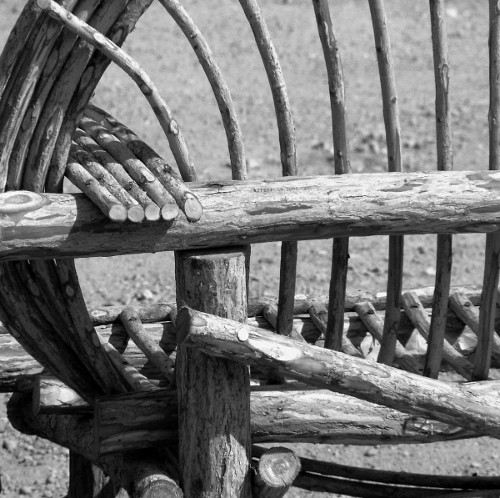
\includegraphics[width=0.95\textwidth]{/part05/wiccom.jpg}
  \begin{center}
    {\large ``WIcker Composition''}\par
    Foto di cobalt123\par
    \url{http://www.flickr.com/photos/cobalt/394252539/}\par
    Licenza: Attribuzione 2.0 Generico (CC BY 2.0)\par
  \end{center}
\clearpage
\cleardoublepage
% (c) 2012 Claudio Carboncini - claudio.carboncini@gmail.com
% (c) 2012-2013 Dimitrios Vrettos - d.vrettos@gmail.com

\chapter{Scomposizione in fattori}

\section{Cosa vuol dire scomporre in fattori}
Scomporre un polinomio in fattori significa scrivere il polinomio come il prodotto di polinomi e monomi che
moltiplicati tra loro danno come risultato il polinomio stesso. Si può paragonare la scomposizione in fattori
di un polinomio alla scomposizione in fattori dei numeri naturali.

\begin{wrapfloat}{figure}{r}{0pt}
 % (c) 2012 Dimitrios Vrettos - d.vrettos@gmail.com
\begin{tikzpicture}[font=\small]
\matrix(a) [matrix of nodes, anchor=west, minimum width=4.5mm]{
36&2\\
18&2\\
9&3\\
3&3\\
1&{}\\};

\draw (a-1-2.north west)--(a-5-2.south west);
\end{tikzpicture}

\end{wrapfloat}

Per esempio, scomporre il numero~$36$ significa scriverlo come~$2^{2}\cdot 3^{2}$ dove~$2$ e~$3$ sono i suoi fattori primi.
Anche~$36 = 9 \cdot 4$ è una scomposizione, ma non è in fattori primi. Allo stesso modo un polinomio va scomposto in fattori non ulteriormente
scomponibili che si chiamano irriducibili. %(questa dovrebbe andare a sinistra della tabella)

Il polinomio~$3a^{3}b^{2}-3ab^{4}$ si può scomporre in fattori in questo modo \[3ab^{2}(a-b)(a+b)\text{,}\] infatti eseguendo i prodotti si
ottiene \[3ab^{2}(a-b)(a+b)=3ab^{2}(a^{2}+ab-ba-b^{2})=3ab^{2}\left(a^{2}-b^{2}\right)=3a^{3}b^{2}-3ab^{4}.\]
La scomposizione termina quando non è possibile scomporre ulteriormente i fattori individuati.
Come per i numeri la scomposizione in fattori dei polinomi identifica il polinomio in maniera univoca (a meno di multipli).

\begin{definizione}
Un polinomio si dice \emph{riducibile} (scomponibile) se può essere scritto come prodotto di due o più polinomi (detti fattori) di grado maggiore di zero.
In caso contrario esso si dirà \emph{irriducibile}.
\end{definizione}

La caratteristica di un polinomio di essere irriducibile dipende dall'insieme numerico al quale appartengono i coefficienti del polinomio;
uno stesso polinomio può essere irriducibile nell'insieme dei numeri razionali, ma riducibile in quello dei numeri reali o
ancora in quello dei complessi.
Dalla definizione consegue che un polinomio di primo grado è irriducibile.

\begin{definizione}
La \emph{scomposizione in fattori di un polinomio} è la sua scrittura come prodotto di fattori irriducibili.
\end{definizione}
\ovalbox{\risolvi \ref{ese:15.1}}

\section{Raccoglimento totale a fattore comune}
Questo è il primo metodo che si deve cercare di utilizzare per scomporre un polinomio.

Il metodo si basa sulla proprietà distributiva della moltiplicazione rispetto all'addizione.

Prendiamo in considerazione il seguente prodotto:~$a(x+y+z)=ax+ay+az$.
Il nostro obiettivo è ora quello di procedere
da destra verso sinistra, cioè avendo il polinomio~$ax+ay+az$ come possiamo fare per individuare il prodotto che lo ha generato?
In questo caso semplice possiamo osservare che i tre monomi contengono tutti la lettera~$a$, che quindi si può mettere in comune,
o come anche si dice ``in evidenza''.
Perciò scriviamo \[ax+ay+az=a(x+y+z).\]

\begin{exrig}
 \begin{esempio}
Analizziamo la scomposizione in fattori~$3a^{2}b\left(2a^{3}-5b^{2}-7c\right)$.
 \begin{equation*}
   \begin{split}
    3a^{2}b\left(2a^{3}-5b^{2}-7c\right) &=3a^{2}b(2a^{3})+3a^{2}b(-5b^{2})+3a^{2}b(-7c)\\
    &=6a^{5}b-15a^{2}b^{3}-21a^{2}bc.
   \end{split}
 \end{equation*}
L'ultima uguaglianza, letta da destra verso sinistra, è il raccoglimento totale a fattore comune.
Partendo da~$6a^{5}b-15a^{2}b^{3}-21a^{2}bc$ possiamo notare che i coefficienti numerici~$6$, $15$ e~$21$ hanno il~$3$ come fattore in comune.
Notiamo anche che la lettera~$a$ è in comune, come la lettera~$b$. Raccogliendo tutti i fattori comuni si avrà il prodotto
$3a^{2}b\left(2a^{3}-5b^{2}-7c\right)$ di partenza.
 \end{esempio}
\end{exrig}

\begin{procedura}
Mettere in evidenza il fattore comune:
\begin{enumeratea}
\item trovare il~$\mcd$ di tutti i termini che formano il polinomio: tutti i fattori in comune con l'esponente minimo con cui compaiono;
\item scrivere il polinomio come prodotto del~$\mcd$ per il polinomio ottenuto dividendo ciascun monomio del polinomio di partenza per il~$\mcd$;
\item verificare la scomposizione eseguendo la moltiplicazione per vedere se il prodotto dà come risultato il polinomio da scomporre.
\end{enumeratea}
\end{procedura}

\begin{exrig}
 \begin{esempio}
Scomporre in fattori~$5a^{2}x^{2}-10ax^{5}$.
  \begin{enumeratea}
  \item Tra i coefficienti numerici il fattore comune è~$5$;
  \item tra la parte letterale sono in comune le lettere~$a$ e~$x$, la~$a$ con esponente~$1$, la~$x$ con esponente~$2$;
  \item pertanto il~$\mcd$ è~$5ax^{2}$;
  \item passiamo quindi a scrivere~$5a^{2}x^{2}-10ax^{5}=5ax^{2}(\ldots \ldots \ldots)$;
  \item nella parentesi vanno i monomi che si ottengono dalle divisioni~$5a^{2}x^{2}:5ax^{2}=a$ e~$-10ax^{5}:5ax^{2}=-2x^{3}$.
  \end{enumeratea}
  In definitiva~$5a^{2}x^{2}-10ax^{5}=5ax^{2}(a-2x^{3})$.
 \end{esempio}

 \begin{esempio}
Scomporre in fattori~$10x^{5}y^{3}z-15x^{3}y^{5}z-20x^{2}y^{3}z^{2}$.
 \begin{enumeratea}
 \item Trovo tutti i fattori comuni con l'esponente minore per formare il~$\mcd$.\, $\mcd=5x^{2}y^{3}z$;
 \item divido ciascun termine del polinomio per~$5x^{2}y^{3}z$:
   \begin{itemize*}
   \item $10x^{5}y^{3}z:5x^{2}y^{3}z=2x^{3}$;
   \item $-15x^{3}y^{5}z:5x^{2}y^{3}z=-3xy^{2}$;
   \item $-20x^{2}y^{3}z^{2}:5x^{2}y^{3}z=-4z$;
   \end{itemize*}
 \item il polinomio si può allora scrivere come~$5x^{2}y^{3}z (2x^{3}-3xy^{2}-4z)$;
 \item Il fattore da raccogliere a fattore comune può essere scelto con il segno~$+$ (positivo) o con il segno~$−$ (negativo).
    Nell'esempio precedente è valida anche la seguente 
    scomposizione:~$10x^{5}y^{3}z-15x^{3}y^{5}z-20x^{2}y^{3}z^{2}=-5x^{2}y^{3}z (-2x^{3}+3xy^{2}+4z)$.
 \end{enumeratea}
 \end{esempio}

 \begin{esempio}
Scomporre in fattori~$-8x^{2}y^{3}+10x^{3}y^{2}$.
 \begin{enumeratea}
  \item Poiché il primo termine è negativo possiamo mettere a fattore comune un 
  numero negativo. Tra~8 e~10 il~$\mcd$ è~2. Tra~$x^{2}y^{3}$ e~$x^{3}y^{2}$ mettiamo 
  a fattore comune le lettere~$x$ e~$y$, entrambe con esponente~$2$, perché è
     il minimo esponente con cui compaiono. In definitiva il monomio da mettere a fattore comune è~$-2x^{2}y^{2}$;
  \item pertanto possiamo cominciare a scrivere~$-2x^{2}y^{2}(\ldots \ldots \ldots)$;
  \item eseguiamo le divisioni~$-8x^{2}y^{3}:(-2x^{2}y^{2})=+4y$ e  $10x^{3}y^{2}:(-2x^{2}y^{2})=-5x$. 
  I quozienti trovati~$+4y$ e~$-5x$ vanno nelle parentesi.
 \end{enumeratea}
 In definitiva~$-8x^{2}y^{3}+10x^{3}y^{2}=-2x^{2}y^{2}(4y-5x)$.
 \end{esempio}

 \begin{esempio}
Scomporre in fattori~$6a(x-1)+7b(x-1)$.
  \begin{enumeratea}
  \item Il fattore comune è~$(x-1)$, quindi il polinomio si può scrivere come~$(x-1)\cdot [\ldots \ldots \ldots]$;
  \item nella parentesi quadra scriviamo i termini che si ottengono dalle divisioni:
   \begin{itemize*}
    \item $6a(x-1):(x-1)=6a$;
    \item $7b(x-1):(x-1)=7b$.
   \end{itemize*}
  \end{enumeratea}
  In definitiva~$6a(x-1)+7b(x-1)=(x-1)(6a+7b)$.
 \end{esempio}

 \begin{esempio}
Scomporre in fattori~$10(x+1)^{2}-5a(x+1)$.
  \begin{enumeratea}
  \item Il fattore comune è~$5(x+1)$, quindi possiamo cominciare a scrivere~$5(x+1)\cdot [\ldots \ldots \ldots]$;
  \item nella parentesi quadra scriviamo i termini che si ottengono dalle divisioni:
   \begin{itemize*}
    \item $10(x+1)^{2}:5(x+1)=2(x+1)$;
    \item $-5a(x+1):5(x+1)=a$.
   \end{itemize*}
  \end{enumeratea}
  In definitiva~$10(x+1)^{2}-5a(x+1)=5(x+1)\bigl[2(x+1)-a \bigr]$.
 \end{esempio}

\end{exrig}

\ovalbox{\risolvii \ref{ese:15.2}, \ref{ese:15.3}, \ref{ese:15.4}, \ref{ese:15.5}, \ref{ese:15.6}, \ref{ese:15.7}, \ref{ese:15.8}, \ref{ese:15.9}, \ref{ese:15.10},\ref{ese:15.11}, \ref{ese:15.12}, \ref{ese:15.13}}

\vspazio\ovalbox{\ref{ese:15.14}}

\section{Raccoglimento parziale a fattore comune}

Quando un polinomio non ha alcun fattore comune a tutti i suoi termini, possiamo provare a mettere in evidenza tra gruppi di monomi
e successivamente individuare il polinomio in comune.

Osserviamo il prodotto~$(a+b)(x+y+z)=ax+ay+az+bx+by+bz$. Supponiamo ora di avere il polinomio
$ax+ay+az+bx+by+bz$ come possiamo fare a tornare indietro per scriverlo come prodotto di polinomi?

%\newpage
\begin{exrig}
 \begin{esempio}
Scomponiamo in fattori~$ax+ay+az+bx+by+bz$. Non c'è nessun fattore comune a tutto il polinomio.

Proviamo a mettere in evidenza per gruppi di termini. Evidenziamo~$a$ tra i primi tre termini e~$b$ tra gli ultimi tre, 
avremo:~$a(x+y+z)+b(x+y+z)$. Ora risulta semplice vedere che il trinomio~$(x+y+z)$ è in comune e quindi lo possiamo mettere 
in evidenza~$ax+ay+az+bx+by+bz=a(x+y+z)+b(x+y+z)=(x+y+z)(a+b)$.
 \end{esempio}
\end{exrig}

\begin{procedura}
Eseguire il raccoglimento parziale.
\begin{enumeratea}
\item Dopo aver verificato che non è possibile effettuare un raccoglimento a fattore comune totale raggruppo i monomi
   in modo che in ogni gruppo sia possibile mettere in comune qualche fattore;
\item verifico se la nuova scrittura del polinomio ha un polinomio (binomio, trinomio, \ldots) comune a tutti i termini;
\item se è presente il fattore comune a tutti i termini lo metto in evidenza;
\item se il fattore comune non è presente la scomposizione è fallita, allora posso provare a raggruppare
   diversamente i monomi o abbandonare questo metodo.
\end{enumeratea}
\end{procedura}

\begin{exrig}
 \begin{esempio}
Scomporre in fattori~$ax+ay+bx+ab$.
  \begin{enumeratea}
  \item Provo a mettere in evidenza la~$a$ nel primo e secondo termine e la~$b$ nel terzo e quarto termine:~$ax+ay+bx+ab=a(x+y)+b(x+a)$;
  \item in questo caso non c'è nessun fattore comune: il metodo è fallito. In effetti il polinomio non si può scomporre in fattori.
  \end{enumeratea}
 \end{esempio}

 \begin{esempio}
Scomporre in fattori~$bx-2ab+2ax-4a^{2}$.
 \begin{enumeratea}
 \item Non vi sono fattori da mettere a fattore comune totale, proviamo con il raccoglimento parziale:~$b$ nei primi due monomi e~$2a$ negli altri due;
 \item $\mmevid{ev_rosso}{bx}-\mmevid{ev_rosso}{2ab}+\mmevid{ev_verde}{2ax}-\mmevid{ev_verde}{4a^{2}}=b(\mmevid{ev_blu}{x-2a})+2a(\mmevid{ev_blu}{x-2a})=(x-2a)(b+2a)$.
%\underline{bx} -\underline{2ab}+\underline{\underline{2ax}}-\underline{\underline{4a^{2}}}=b(\underline{x-2a})+2a(\underline{x-2a})=(x-2a)(b+2a)$.
 \end{enumeratea}
 \end{esempio}

 \begin{esempio}
Scomporre in fattori~$bx^{3}+2x^{2}-bx-2+abx+2a$.
 \begin{enumeratea}

 \item Raggruppiamo nel seguente modo:~$\mmevid{ev_rosso}{bx^{3}}+\mmevid{ev_verde}{2x^{2}}-\mmevid{ev_rosso}{bx}-\mmevid{ev_verde}{2}+\mmevid{ev_rosso}{abx}+\mmevid{ev_verde}{2a}$ tra quelli evidenziati in \evid{ev_rosso}{\phantom{I}} mettiamo a fattore comune~$bx$ e tra quelli evidenziati in \evid{ev_verde}{\phantom{I}} mettiamo a fattore comune~$2$;

% \item Raggruppiamo nel seguente modo:~$\underline{bx^{3}}+\underline{\underline {2x^{2}}}-\underline{bx}-\underline{\underline~2}
%     +\underline{abx}+\underline{\underline{2a}}$ tra quelli con sottolineatura semplice metto a fattore comune~$bx$, tra quelli
%     con doppia sottolineatura metto a fattore comune~$2$;

 \item $\mmevid{ev_rosso}{bx^{3}}+\mmevid{ev_verde}{2x^{2}}-\mmevid{ev_rosso}{bx}-\mmevid{ev_verde}{2}+\mmevid{ev_rosso}{abx}+\mmevid{ev_verde}{2a}=bx\bigl(\mmevid{ev_blu}{x^{2}-1+a}\bigr)+2\bigl(\mmevid{ev_blu}{x^{2}-1+a}\bigr)=\bigl(x^{2}-1+a\bigr)\bigl(bx+2\bigr)$.

%  \item $\underline{bx^{3}}+\underline{\underline {2x^{2}}}-\underline{bx}-\underline{\underline~2}+\underline{abx}+\underline{\underline{2a}}
%     =bx\bigl(\underline{x^{2}-1+a}\bigr)+2\bigl(\underline{x^{2}-1+a}\bigr)=\bigl(x^{2}-1+a\bigr)\bigl(bx+2\bigr)$.
 \end{enumeratea}
 \end{esempio}

 \begin{esempio}
Scomporre in fattori~$5ab^{2}-10abc-25abx+50acx$.
 \begin{enumeratea}
  \item Il fattore comune è~$5a$, quindi:
    \begin{itemize*}
    \item $5ab^{2}-10abc-25abx+50acx=5a\bigl(b^{2}-2bc-5bx+10cx\bigr)$;
    \end{itemize*}
  \item vediamo se è possibile scomporre il polinomio in parentesi con un raccoglimento parziale~$5a(\mmevid{ev_rosso}{b^{2}}-\mmevid{ev_rosso}{2bc}-\mmevid{ev_verde}{5bx}+\mmevid{ev_verde}{10cx})=5a\bigl[b(\mmevid{ev_blu}{b-2c})-5x(\mmevid{ev_blu}{b-2c})\bigr]=5a(b-2c)(b-5x)$.

%  \item vediamo se è possibile scomporre il polinomio in parentesi con un raccoglimento parziale~$5a(\underline{b^{2}}-\underline{2bc}
%     -\underline{\underline{5bx}}+\underline{\underline{10cx}})=5a\bigl[b(\underline{b-2c})-5x(\underline{b-2c})\bigr]=5a(b-2c)(b-5x)$.
 \end{enumeratea}
 \end{esempio}
\end{exrig}

\ovalbox{\risolvii \ref{ese:15.16}, \ref{ese:15.17}, \ref{ese:15.18}, \ref{ese:15.19}, \ref{ese:15.20}, \ref{ese:15.21}, \ref{ese:15.22}, \ref{ese:15.23}, \ref{ese:15.24},\ref{ese:15.25}, \ref{ese:15.26}}

\ovalbox{\ref{ese:15.27}, \ref{ese:15.28}}

\newpage
% (c) 2012 Claudio Carboncini - claudio.carboncini@gmail.com
% (c) 2012 -2014 Dimitrios Vrettos - d.vrettos@gmail.com

\section{Esercizi}
\subsection{Esercizi dei singoli paragrafi}
\subsubsection*{15.1 - Identità ed equazioni}

\begin{esercizio}
\label{ese:15.1}
Risolvi in~$\insZ$ la seguente equazione:~$-x+3=-1$.

\emph{Suggerimento}. Lo schema operativo è: entra~$x$, cambia il segno in~$-x$, aggiunge~$3$, si ottiene~$-1$.
Ora ricostruisci il cammino inverso: da~$-1$ togli~$3$ ottieni \ldots cambia segno ottieni come soluzione~$x = \ldots$.
\end{esercizio}

\subsubsection*{15.3 - Equazioni intere}

\begin{esercizio}[\Ast]
\label{ese:15.2}
Risolvi le seguenti equazioni applicando il~1° principio di equivalenza.
\begin{multicols}{3}
\begin{enumeratea}
%\spazielenx
 \item $x+2=7$;
 \item $2+x=3$;
 \item $16+x=26$;
 \item $x-1=1$;
 \item $3+x=-5$;
 \item $12+x=-22$;
 \item $3x=2x-1$;
 \item $8x=7x+4$;
 \item $2x=x-1$;
 \item $5x=4x+2$;
 \item $3x=2x-3$;
 \item $3x=2x-2$.
\end{enumeratea}
\end{multicols}
\end{esercizio}

\begin{esercizio}[\Ast]
\label{ese:15.3}
Risolvi le seguenti equazioni applicando il~1° principio di equivalenza.
\begin{multicols}{3}
\begin{enumeratea}
%\spazielenx
 \item $7+x=0$;
 \item $7=-x$;
 \item $-7=x$;
 \item $1+x=0$;
 \item $1-x=0$;
 \item $0=2-x$;
 \item $3x-1=2x-3$;
 \item $7x-2x-2=4x-1$;
 \item $-5x+2=-6x+6$;
 \item $-2+5x=8+4x$;
 \item $7x+1=6x+2$;
 \item $-1-5x=3-6x$.
\end{enumeratea}
\end{multicols}
\end{esercizio}

\begin{esercizio}[\Ast]
\label{ese:15.4}
Risolvi le seguenti equazioni applicando il~2° principio di equivalenza.
\begin{multicols}{3}
\begin{enumeratea}
%\spazielenx
 \item $2x=8$;
 \item $2x=3$;
 \item $6x=24$;
 \item $0x=1$;
 \item $\dfrac{1}{3}x=-1$;
 \item $\dfrac{1}{2}x=\dfrac{1}{4}$;
 \item $\dfrac{3}{2}x=12$;
 \item $2x=-2$;
 \item $3x=\dfrac{1}{6}$;
 \item $\dfrac{1}{2}x=4$;
 \item $\dfrac{3}{4}x=\dfrac{12}{15}$;
 \item $2x=\dfrac{1}{2}$.
\end{enumeratea}
\end{multicols}
\end{esercizio}

\begin{esercizio}[\Ast]
\label{ese:15.5}
Risolvi le seguenti equazioni applicando il~2° principio di equivalenza.
\begin{multicols}{4}
\begin{enumeratea}
%\spazielenx
 \item $3x=6$;
 \item $\dfrac{1}{3}x=\dfrac{1}{3}$;
 \item $\dfrac{2}{5}x=\dfrac{10}{25}$;
 \item $-{\dfrac{1}{2}}x=-{\dfrac{1}{2}}$;
 \item $\np{0,1}x=1$;
 \item $\np{0,1}x=10$;
 \item $\np{0,1}x=\np{0,5}$;
 \item $\np{-0,2}x=5$;
 \item $\dfrac{1}{2}x=2$;
 \item $2x=\dfrac{1}{2}$;
 \item $\dfrac{1}{2}x=\dfrac{1}{2}$;
 \item $2x=2$.
\end{enumeratea}
\end{multicols}
\end{esercizio}

\begin{esercizio}[\Ast]
\label{ese:15.6}
Risolvi le seguenti equazioni applicando entrambi i principi.
\begin{multicols}{3}
\begin{enumeratea}
%\spazielenx
 \item $2x+1=7$;
 \item $3-2x=3$;
 \item $6x-12=24$;
 \item $3x+3=4$;
 \item $5-x=1$;
 \item $7x-2=5$;
 \item $2x+8=8-x$;
 \item $2x-3=3-2x$;
 \item $6x+24=3x+12$;
 \item $2+8x=6-2x$;
 \item $6x-6=5-x$;
 \item $-3x+12=3x+18$.
\end{enumeratea}
\end{multicols}
\end{esercizio}

\begin{esercizio}[\Ast]
\label{ese:15.7}
Risolvi le seguenti equazioni applicando entrambi i principi.
\begin{multicols}{3}
\begin{enumeratea}
%\spazielenx
 \item $3-2x=8+2x$;
 \item $\dfrac{2}{3}x-3=\dfrac{1}{3}x+1$;
 \item $\dfrac{6}{5}x=\dfrac{24}{5}-x$;
 \item $3x-2x+1=2+3x-1$;
 \item $\dfrac{2}{5}x-\dfrac{3}{2}=\dfrac{3}{2}x+\dfrac{1}{10}$;
 \item $\dfrac{5}{6}x+\dfrac{3}{2}=\dfrac{25}{3}-\dfrac{10}{2}x$;
 \item $7x+4=5x+7$;
 \item $\dfrac{x}{2}-2=\dfrac{1}{7}+\dfrac{x}{7}$;
 \item $\dfrac{2}{3}x+\dfrac{2}{3}=x+2$;
 \item $\dfrac{4}{5}x-\dfrac{2}{3}=\dfrac{3}{2}x+\dfrac{1}{30}$;
 \item $\dfrac{1}{6}x+\dfrac{1}{6}=\dfrac{1}{3}+\dfrac{3}{2}x$;
 \item $-\dfrac{1}{12}-\dfrac{x}{4}=-\dfrac{9}{30}x-\dfrac{1}{30}$.
\end{enumeratea}
\end{multicols}
\end{esercizio}

\begin{esercizio}[\Ast]
\label{ese:15.8}
Risolvi le seguenti equazioni nell'insieme a fianco indicato.
\begin{multicols}{3}
\begin{enumeratea}
%\spazielenx
 \item $x+7=8\quad$ in $\insN$;
 \item $4+x=2\quad$ in $\insZ$;
 \item $x-3=4\quad$ in $\insN$;
 \item $x=0\quad$ in $\insN$;
 \item $x+1=0\quad$ in $\insZ$;
 \item $5x=0\quad$ in $\insZ$;
 \item $\dfrac{x}{4}=0$ in $\insQ$;
 \item $-x=0\quad$ in $\insZ$;
 \item $7+x=0\quad$ in $\insZ$;
 \item $-2x=0\quad$ in $\insZ$;
 \item $-x-1=0\quad$ in $\insZ$;
 \item $\dfrac{-x}{4}=0\quad$ in $\insQ$.
\end{enumeratea}
\end{multicols}
\end{esercizio}

\begin{esercizio}[\Ast]
\label{ese:15.9}
Risolvi le seguenti equazioni nell'insieme a fianco indicato.
\begin{multicols}{3}
\begin{enumeratea}
%\spazielenx
 \item $x-\dfrac{2}{3}=0\quad$ in $\insQ$;
 \item $\dfrac{x}{-3}=0\quad$ in $\insZ$;
 \item $2(x-1)=0\quad$ in $\insZ$;
 \item $-3x=1\quad$ in $\insQ$;
 \item $3x=-1\quad$ in $\insQ$;
 \item $\dfrac{x}{3}=1\quad$ in $\insQ$;
 \item $\dfrac{x}{3}=2\quad$ in $\insQ$;
 \item $\dfrac{x}{3}=-2\quad$ in $\insQ$;
 \item $0x=0\quad$ in $\insQ$;
 \item $0x=5\quad$ in $\insQ$;
 \item $0x=-5\quad$ in $\insQ$;
 \item $\dfrac{x}{1}=0\quad$ in $\insQ$.
\end{enumeratea}
\end{multicols}
\end{esercizio}

\begin{esercizio}[\Ast]
\label{ese:15.10}
Risolvi le seguenti equazioni nell'insieme a fianco indicato.
\begin{multicols}{3}
\begin{enumeratea}
%\spazielenx
 \item $\dfrac{x}{1}=1\quad$ in $\insQ$;
 \item $-x=10\quad$ in $\insZ$;
 \item $\dfrac{x}{-1}=-1\quad$ in $\insZ$;
 \item $3x=3\quad$ in $\insN$;
 \item $-5x=2\quad$ in $\insZ$;
 \item $3x+2=0\quad$ in $\insQ$;
 \item $3x=\dfrac{1}{3}$ in $\insQ$;
 \item $-3x=-{\dfrac{1}{3}}$ in $\insQ$;
 \item $x+2=0$ in $\insQ$;
 \item $4x-4=0$ in $\insQ$;
 \item $4x-0=1$ in $\insQ$;
 \item $2x+3=x+3$ in $\insQ$.
\end{enumeratea}
\end{multicols}
\end{esercizio}

\begin{esercizio}
\label{ese:15.11}
Risolvi le seguenti equazioni nell'insieme~$\insQ$.
\begin{multicols}{3}
\begin{enumeratea}
%\spazielenx
 \item $4x-4=1$;
 \item $4x-1=1$;
 \item $4x-1=0$;
 \item $3x=12-x$;
 \item $4x-8=3x$;
 \item $-x-2=-2x-3$;
 \item $-3(x-2)=3$;
 \item $x+2=2x+3$;
 \item $-x+2=2x+3$;
 \item $3(x-2)=0$;
 \item $3(x-2)=1$;
 \item $3(x-2)=3$.
\end{enumeratea}
\end{multicols}
\end{esercizio}

\begin{esercizio}[\Ast]
\label{ese:15.12}
Risolvi le seguenti equazioni nell'insieme~$\insQ$.
\begin{multicols}{3}
\begin{enumeratea}
%\spazielenx
 \item $0(x-2)=1$;
 \item $0(x-2)=0$;
 \item $12+x=-9x$;
 \item $40x+3=30x-100$;
 \item $4x+8x=12x-8$;
 \item $\dfrac{x+1}{2}=x+1$.
\end{enumeratea}
\end{multicols}
\end{esercizio}

\pagebreak

\begin{esercizio}
\label{ese:15.13}
Risolvi l'equazione~$10x+4=-2\cdot (x+5)-x$ seguendo la traccia:
\begin{enumeratea}
%\spazielenx
 \item svolgi i calcoli al primo e al secondo membro: \dotfill;
 \item somma i monomi simili in ciascun membro dell'equazione: \dotfill;
 \item applica il primo principio d'equivalenza per lasciare in un membro solo monomi con l'incognita e nell'altro membro solo numeri: \dotfill;
 \item somma i termini del primo membro e somma i termini del secondo membro: \dotfill;
 \item applica il secondo principio d'equivalenza dividendo ambo i membri per il coefficiente dell'incognita: \dotfill in forma canonica: \dotfill;
 \item scrivi l'Insieme Soluzione:~$\IS = \ldots \ldots \ldots$.
\end{enumeratea}
\end{esercizio}

\begin{esercizio}
\label{ese:15.14}
Risolvi, seguendo la traccia, l'equazione~$x-(3x+5)=(4x+8)-4\cdot (x+1)$:
\begin{enumeratea}
%\spazielenx
 \item svolgi i calcoli: \dotfill;
 \item somma i monomi simili: \dotfill;
 \item porta al primo membro i monomi con la~$x$ e al secondo quelli senza:~$\dotfill$;
 \item somma i monomi simili al primo membro e al secondo membro:~$\dotfill$;
 \item dividi ambo i membri per il coefficiente dell'incognita:~$\dotfill$;
 \item l'insieme soluzione è:~$\dotfill$
\end{enumeratea}
\end{esercizio}

\begin{esercizio}[\Ast]
\label{ese:15.15}
Risolvi le seguenti equazioni.
\begin{multicols}{2}
 \begin{enumeratea}
 \item $3(x-1)+2(x-2)+1=2x$;
 \item $x-(2x+2)=3x-(x+2)-1$;
 \item $-2(x+1)-3(x-2)=6x+2$;
 \item $x+2-3(x+2)=x-2$.
 \end{enumeratea}
\end{multicols}
\end{esercizio}

\begin{esercizio}[\Ast]
\label{ese:15.16}
Risolvi le seguenti equazioni.
\begin{multicols}{2}
 \begin{enumeratea}
 \item $2(1-x)-(x+2)=4x-3(2-x)$;
 \item $(x+2)^{2}=x^{2}-4x+4$;
 \item $5(3x-1)-7(2x-4)=28$;
 \item $(x+1)(x-1)+2x=5+x(2+x)$.
 \end{enumeratea}
\end{multicols}
\end{esercizio}

\begin{esercizio}[\Ast]
\label{ese:15.17}
Risolvi le seguenti equazioni.
 \begin{enumeratea}
 \item $12x-3(2x-1)=-4(1-x)-1$;
 \item $3(x-2)+5(x+1)=2(2x+7)+4x+8$;
 \item $3(2x+1)-4x+3=2(3x+1)-4(x-1)$;
 \item $4(x-2)^{2}-(2x+1)^{2}=-12x-19$.
 \end{enumeratea}
\end{esercizio}

\begin{esercizio}[\Ast]
\label{ese:15.18}
Risolvi le seguenti equazioni.
 \begin{enumeratea}
 \item $2x+(x+2)(x-2)+5=(x+1)^{2}$;
 \item $4(x-2)+3(x+2)=2(x-1)-(x+1)$;
 \item $(x+2)(x+3)-(x+3)^{2}=(x+1)(x-1)-x(x+1)$;
 \item $x^{3}+6x^{2}+(x+2)^{3}+11x+(x+2)^{2}=(x+3)\left(2x^{2}+7x\right)$.
 \end{enumeratea}
\end{esercizio}

\begin{esercizio}[\Ast]
\label{ese:15.19}
Risolvi le seguenti equazioni.
 \begin{enumeratea}
 \item $(x+2)^{3}-(x-1)^{3}=9(x+1)^{2}-9x$;
 \item $(x+1)^{2}+2x+2(x-1)=(x+2)^{2}$;
 \item $2(x-2)(x+3)-3(x+1)(x-4)=-9(x-2)^{2}+\left(8x^{2}-25x+36\right)$;
 \item $(2x+3)^{2}+x^{2}+1=(2x-3)^{2}+x(x+3)$.
 \end{enumeratea}
\end{esercizio}

\begin{esercizio}[\Ast]
\label{ese:15.20}
Risolvi le seguenti equazioni.
 \begin{enumeratea}
 \item $(2x-3)^{2}-4x(2-5x)-4=8x(3x+4)$;
 \item $(x-1)\left(x^{2}+x+1\right)-3x^{2}=(x-1)^{3}+1$;
 \item $(2x-1)\left(4x^{2}+2x+1\right)=(2x-1)^{3}+12x^{2}$;
 \item $20x-1=(3x-8)^{2}-(5x-9)^{2}+(5-4x)^{2}$.
 \end{enumeratea}
\end{esercizio}

\begin{esercizio}[\Ast]
\label{ese:15.21}
Risolvi le seguenti equazioni con le regole pratiche indicate.
 \begin{enumeratea}
 \item $(3x-2)^{2}+(2x+5)^{2}=(13x-2)(x+1)$;
 \item $(2x+1)^{2}(x-3)^{2}=\left(2x^{2}+1\right)^{2}+x^{2}(9-20x)+8$;
 \item $3(x-1)^{2}(x+2)+3(x-1)(x+2)^{2}+(x+2)^{3}-4x^{2}(2x+3)+x=1-(x-1)^{3}$;
 \item $\left(16x^{2}-1\right)-(3x+1)(3x+1)=(3x+1)(2x-2)+(x-1)^{2}$.
 \end{enumeratea}
\end{esercizio}

\begin{esercizio}[\Ast]
\label{ese:15.22}
Risolvi le seguenti equazioni con le regole pratiche indicate.
 \begin{enumeratea}
 \item $2(x+1)-3x=7(x-3)-5(x+2)$;
 \item $3(4-x)-6(3-x)=10(x-1)-5(x-2)$;
 \item $21-5x^{2}=(2x-5)^{2}-(4-3x)^{2}$;
 \item $(3-x)(1-x)-(2-x)(x-1)=2(2-x)(3-x)-(7-3x)$;
 \item $4\big[(3x-1)x+2x-2\big]=10x+3x\big[(x+1)2-4+2x\big]$.
% \item $\dfrac{3(x+1)}{2}+2-\left(3+\dfrac{1+x}{6}\right)=\dfrac{5x+8}{3}-\left(\dfrac{3x-1}{2}-3\right)$.
 \end{enumeratea}
\end{esercizio}

\subsubsection*{15.4 - Equazioni a coefficienti frazionari}

\begin{esercizio}[\Ast]
\label{ese:15.23}
Risolvi l'equazione~$\dfrac{3\cdot (x-11)}{4}=\dfrac{3\cdot (x+1)}{5}-\dfrac{1}{10}$.
\begin{enumerate}
%\spazielenx
 \item calcola~$\mcm(4\text{,~}5\text{,~}10) = \ldots \ldots$;
 \item moltiplica ambo i membri per \dotfill e ottieni: \dotfill;
 \item \dotfill
\end{enumerate}
\end{esercizio}

\begin{esercizio}
\label{ese:15.24}
Risolvi le seguenti equazioni nell'insieme~$\insQ$.
\begin{multicols}{3}
\begin{enumeratea}
%\spazielenx
 \item $2x+2=2x+3$;
 \item $\dfrac{x+2}{2}=\dfrac{x+1}{2}$;
 \item $\dfrac{2x+1}{2}=x+1$;
 \item $\dfrac{x}{2}+\dfrac{1}{4}=3x-\dfrac{1}{2}$;
 \item $\pi x=0$;
 \item $2\pi x=\pi$.
\end{enumeratea}
\end{multicols}
\end{esercizio}

\begin{esercizio}
\label{ese:15.25}
Risolvi le seguenti equazioni nell'insieme~$\insQ$.
\begin{multicols}{2}
\begin{enumeratea}
%\spazielenx
 \item $\np{0,12}x=\np{0,1}$;
 \item $-{\dfrac{1}{2}}x-\np{0,3}=-{\dfrac{2}{5}}x-\np{0,15}$;
 \item $892x-892=892x-892$;
 \item $892x-892=893x-892$;
 \item $348x-347=340x-347$;
 \item $340x+740=\np{8942}+340x$.
\end{enumeratea}
\end{multicols}
\end{esercizio}

\begin{esercizio}
\label{ese:15.26}
Risolvi le seguenti equazioni nell'insieme~$\insQ$.
\begin{multicols}{3}
\begin{enumeratea}
%\spazielenx
 \item $2x+3=2x+4$;
 \item $2x+3=2x+3$;
 \item $2(x+3)=2x+5$;
 \item $2(x+4)=2x+8$;
 \item $3x+6=6x+6$;
 \item $-2x+3=-2x+4$.
\end{enumeratea}
\end{multicols}
\end{esercizio}

\begin{esercizio}
\label{ese:15.27}
Risolvi le seguenti equazioni nell'insieme~$\insQ$.
\begin{multicols}{2}
\begin{enumeratea}
%\spazielenx
 \item $\dfrac{x}{2}+\dfrac{1}{4}=\dfrac{x}{4}-\dfrac{1}{2}$;
 \item $\dfrac{x}{2}+\dfrac{1}{4}=\dfrac{x}{2}-\dfrac{1}{2}$;
 \item $\dfrac{x}{2}+\dfrac{1}{4}=3\dfrac{x}{2}-\dfrac{1}{2}$;
 \item $\dfrac{x}{200}+\dfrac{1}{100}=\dfrac{1}{200}$;
 \item $\np{1000}x-100=\np{2000}x-200$;
 \item $100x-\np{1000}=\np{-1000}x+100$.
\end{enumeratea}
\end{multicols}
\end{esercizio}

\begin{esercizio}[\Ast]
\label{ese:15.28}
Risolvi le seguenti equazioni nell'insieme~$\insQ$.
\begin{multicols}{2}
\begin{enumeratea}
%\spazielenx
 \item $x-5(1-x)=5+5x$;
 \item $2(x-5)-(1-x)=3x$;
 \item $3(2+x)=5(1+x)-3(2-x)$;
 \item $4(x-2)-3(x+2)=2(x-1)$;
 \item $\dfrac{x+\np{1000}}{3}+\dfrac{x+\np{1000}}{4}=1$;
 \item $\dfrac{x-4}{5}=\dfrac{2x+1}{3}$.
\end{enumeratea}
\end{multicols}
\end{esercizio}

\begin{esercizio}[\Ast]
\label{ese:15.29}
Risolvi le seguenti equazioni nell'insieme~$\insQ$.
\begin{multicols}{2}
\begin{enumeratea}
%\spazielenx
 \item $\dfrac{x+1}{2}+\dfrac{x-1}{5}=\dfrac{1}{10}$;
 \item $\dfrac{x}{3}-\dfrac{1}{2}\;=\;\dfrac{x}{4}-\dfrac{x}{6}$;
 \item $8x-\dfrac{x}{6}=2x+11$;
 \item $3(x-1)-\dfrac{1}{7}=4(x-2)+1$;
 \item $537x+537\dfrac{x}{4}-\dfrac{537x}{7}=0$;
 \item $\dfrac{2x+3}{5}=x-1$.
\end{enumeratea}
\end{multicols}
\end{esercizio}

\begin{esercizio}[\Ast]
\label{ese:15.30}
Risolvi le seguenti equazioni nell'insieme~$\insQ$.
\begin{multicols}{2}
\begin{enumeratea}
\spazielenx
 \item $\dfrac{x}{2}-\dfrac{x}{6}-1=\dfrac{x}{3}$;
 \item $\dfrac{4-x}{5}+\dfrac{3-4x}{2}=3$;
 \item $\dfrac{x+3}{2}=3x-2$;
 \item $\dfrac{x+\np{0,25}}{5}=\np{1,75}-\np{0,}\overline{{3}}x$;
 \item $3(x-2)-4(5-x)=3x\left(1-\dfrac{1}{3}\right)$;
 \item $4(2x-1)+5=1-2(-3x-6)$.
\end{enumeratea}
\end{multicols}
\end{esercizio}

\begin{esercizio}[\Ast]
\label{ese:15.31}
Risolvi le seguenti equazioni nell'insieme~$\insQ$.
\begin{multicols}{2}
\begin{enumeratea}
%\spazielenx
 \item $\dfrac{3}{2}(x+1)-\dfrac{1}{3}(1-x)=x+2$;
 \item $\dfrac{1}{2}(x+5)-x=\dfrac{1}{2}(3-x)$;
 \item $(x+3)^{2}=(x-2)(x+2)+\dfrac{1}{3}x$;
 \item $\dfrac{(x+1)^{2}}{4}-\dfrac{2+3x}{2}=\dfrac{(x-1)^{2}}{4}$;
 \item $2\left(x-\dfrac{1}{3}\right)+x=3x-2$;
 \item $\dfrac{3}{4}-\dfrac{x}{3}=\dfrac{1-x}{3}$.
\end{enumeratea}
\end{multicols}
\end{esercizio}

\begin{esercizio}[\Ast]
\label{ese:15.32}
Risolvi le seguenti equazioni nell'insieme~$\insQ$.
\begin{multicols}{2}
\begin{enumeratea}
%\spazielenx
 \item $\dfrac{1}{6}=\dfrac{1}{2}x-\dfrac{1}{3}x$;
 \item $\dfrac{x+2}{3}=-\left(1+\dfrac{x}{2}\right)$;
 \item $\dfrac{5x-1}{3}-x=4x-\dfrac{1}{3}$;
 \item $\dfrac{3x-8}{2}=4+3x$;
 \item $2-\dfrac{5+x}{2}=\dfrac{1-x}{3}$;
 \item $\dfrac{3}{4}-\dfrac{x}{3}=\dfrac{x-2}{2}$.
\end{enumeratea}
\end{multicols}
\end{esercizio}

\begin{esercizio}[\Ast]
\label{ese:15.33}
Risolvi le seguenti equazioni nell'insieme~$\insQ$.
\begin{multicols}{2}
\begin{enumeratea}
%\spazielenx
 \item $(2x-3)(5+x)+\dfrac{1}{4}=2(x-1)^{2}-\dfrac{1}{2}$;
 \item $(x-2)(x+5)+\dfrac{1}{4}=x^{2}-\dfrac{1}{2}$;
 \item $\left(x-\dfrac{1}{2}\right)\left(x-\dfrac{1}{2}\right)=x^{2}+\dfrac{1}{2}$;
 \item $(x+1)^{2}=(x-1)^{2}$;
 \item $\dfrac{(1-x)^{2}}{2}-\dfrac{x^{2}-1}{2}=1$;
 \item $\dfrac{(x+1)^{2}}{3}=\dfrac{1}{3}(x^{2}-1)$.
\end{enumeratea}
\end{multicols}
\end{esercizio}

\begin{esercizio}[\Ast]
\label{ese:15.34}
Risolvi le seguenti equazioni nell'insieme~$\insQ$.
\begin{enumeratea}
%\spazielenx
 \item $4(x+1)-3x(1-x)=(x+1)(x-1)+4+2x^{2}$;
 \item $\dfrac{1-x}{3}\cdot (x+1)=1-x^{2}+\dfrac{2}{3}\left(x^{2}-1\right)$;
 \item $(x+1)^{2}=x^{2}-1$;
 \item $(x+1)^{3}=(x+2)^{3}-3x(x+3)$;
 \item $\dfrac{1}{3}x\left(\dfrac{1}{3}x-1\right)+\dfrac{5}{3}x\left(1+\dfrac{1}{3}x\right)=\dfrac{2}{3}x(x+3)$;
 \item $\dfrac{1}{2}\left(3x+\dfrac{1}{3}\right)-(1-x)+2\left(\dfrac{1}{3}x-1\right)=-{\dfrac{3}{2}}x+1$.
\end{enumeratea}
\end{esercizio}

\begin{esercizio}[\Ast]
\label{ese:15.35}
Risolvi le seguenti equazioni nell'insieme~$\insQ$.
\begin{enumeratea}
%\spazielenx
 \item $3+2x-\dfrac{1}{2}\left(\dfrac{x}{2}+1\right)-\dfrac{3}{4}x=\dfrac{3}{4}x+\dfrac{x+3}{2}$;
 \item $\dfrac{1}{2}\left[\dfrac{x+2}{2}-\left(x+\dfrac{1}{2}\right)+\dfrac{x+1}{2}\right]+\dfrac{1}{4}x=\dfrac{x-2}{4}-\left(x+\dfrac{2-x}{3}\right)$;
 \item $2\left(x-\dfrac{1}{2}\right)^{2}+\left(x+\dfrac{1}{2}\right)^{2}=(x+1)(3x-1)-5x-\dfrac{1}{2}$;
 \item $\dfrac{2\left(x-1\right)}{3}+\dfrac{x+1}{5}-\dfrac{3}{5}=\dfrac{x-1}{5}+\dfrac{7}{15}x$;
 \item $\dfrac{1}{2}(x-2)-\left(\dfrac{x+1}{2}-\dfrac{1+x}{2}\right)=\dfrac{1}{2}-\dfrac{2-x}{6}+\dfrac{1+x}{3}$;
 \item $-\left(\dfrac{1}{2}x+3\right)-\dfrac{1}{2}\left(x+\dfrac{5}{2}\right)+\dfrac{3}{4}(4x+1)=\dfrac{1}{2}(x-1)$.
\end{enumeratea}
\end{esercizio}

\begin{esercizio}[\Ast]
\label{ese:15.36}
Risolvi le seguenti equazioni nell'insieme~$\insQ$.
\begin{enumeratea}
%\spazielenx
 \item $\dfrac{(x+1)(x-1)}{9}-\dfrac{3x-3}{6}=\dfrac{(x-1)^{2}}{9}-\dfrac{2-2x}{6}$;
 \item $\left(x-\dfrac{1}{2}\right)^{3}-\left(x+\dfrac{1}{2}\right)^{2}-x(x+1)(x-1)=\dfrac{-5}{2}x(x+1)$;
 \item $\dfrac{1}{2}\left(3x-\dfrac{1}{3}\right)-\dfrac{1}{3}(1+x)(-1+x)+3\left(\dfrac{1}{3}x-1\right)^{2}=\dfrac{2}{3}x$;
 \item $(x-2)(x-3)-6=(x+2)^2 +5$;
 \item $(x-3)(x-4)-\dfrac{1}{3}(1-3x)(2-x)=\dfrac{1}{3}x-5\left(\dfrac{2x-9}{6}\right)$;
 \item $\dfrac{2w-1}{3}+\dfrac{w-5}{4}=\dfrac{w+1}{3}-4$.
\end{enumeratea}
\end{esercizio}

\pagebreak

\begin{esercizio}[\Ast]
\label{ese:15.37}
Risolvi le seguenti equazioni nell'insieme~$\insQ$.
\begin{enumeratea}
%\spazielenx
 \item $\dfrac{2}{3}\left(x-\dfrac{3}{2}\right)+\dfrac{5}{2}\left(\dfrac{x}{5}-\dfrac{2}{3}\right)=\dfrac{2}{3}+x+5$;
 \item $\dfrac{12x-\dfrac{1}{2}}{3}-2(2x-3)=\dfrac{37}{6}$;
 \item $\dfrac{1}{2}(x-3)+\dfrac{1}{3}x=\dfrac{1}{2}\left(x-\dfrac{1}{3}\right)$;
 \item $3x-1+\dfrac{3(3x-1)}{5}=\dfrac{7x+4}{5}+2x$;
 \item $\dfrac{1}{4}(1+5x)+\dfrac{5}{6}+\dfrac{1}{9}(3x-2)^{2}=2x-\dfrac{(1+3x)(2-3x)}{9}$;
 \item $\dfrac{3x-2}{3}+\dfrac{1-8x}{6}+\dfrac{1}{3}(x+3)=-\dfrac{x+3}{4}$.
\end{enumeratea}
\end{esercizio}

\begin{esercizio}[\Ast]
\label{ese:15.38}
Risolvi le seguenti equazioni nell'insieme~$\insQ$.
\begin{enumeratea}
%\spazielenx
 \item $2x-\left[\dfrac{x-2}{3}-\dfrac{1-x}{3}-\left(\dfrac{1+2x}{2}+5x\right)\right]=\dfrac{3}{2}$;
 \item $\dfrac{3\left(\dfrac{1}{3}-2x\right)-2(1-x)}{4}+\dfrac{\dfrac{2}{3}+\dfrac{x}{2}}{2}-\dfrac{1}{12}(1+8x)=0$;
 \item $\dfrac{1}{3}=\left\lbrace\dfrac{1}{3}\left[\dfrac{1}{3}\left(\dfrac{x}{3}+2\right)\right]+2 \right\rbrace\dfrac{1}{9}$;
 \item $(1+3x)^{2}+x(14+x)+24=(5+2x)^{2}-2x\big[3x-2(3x-1)-2\big]$;
 \item $(1-x)^{2}+\dfrac{5x+20}{5}-\dfrac{1+x}{7}=4+x-x(2-x)$;
 \item $\dfrac{(2-x)(1-3x)}{4}-\dfrac{5x^{2}}{12}=\dfrac{(3-x)^{2}}{3}-\dfrac{x+3}{12}$.
\end{enumeratea}
\end{esercizio}

\begin{esercizio}[\Ast]
\label{ese:15.39}
Risolvi le seguenti equazioni nell'insieme~$\insQ$.
\begin{enumeratea}
%\spazielenx
 \item $(2x-5)^2 +2(x-3)=(4x-2)(x+3)-28x+25$;
 \item $\dfrac{(x-3)(x+3)+(x-2)(2-x)-3(x-2)}{\dfrac{1}{3}-3}=\dfrac{\dfrac{2}{3}x+\dfrac{1}{2}x}{2}$;
 \item $2\left(\dfrac{1}{2}x-1\right)^{2}-\dfrac{(x+2)(x-2)}{2}+2x=x+\dfrac{1}{2}$;
 \item $\left(\np{0,}\overline{{1}}x-10\right)^{2}+\np{0,1}(x-\np{0,2})+\left(\dfrac{1}{3}x+\np{0,3}\right)^{2}=\dfrac{10}{81}x^{2}+\np{0,07}$;
 \item $5x+\dfrac{1}{6}-\left(\dfrac{2x+1}{2}\right)^{2}+\left(\dfrac{3x-1}{3}\right)^{2}+\dfrac{1}{3}x+(2x-1)(2x+1)=(2x+1)^{2}+\dfrac{1}{36}$;
 \item \begin{multline*}\left(1+\dfrac{1}{2}x\right)^{3}-2\left(\dfrac{1}{2}x-2\right)^{2}+\left(\dfrac{3x-1}{3}\right)^{2}-\left(1-\dfrac{1}{3}x\right)x+\dfrac{1}{3}x={\dfrac{1}{3}}(2x+1)^{2} \\
     +\dfrac{1}{4}x^{2}-\dfrac{5}{9}+\dfrac{1}{2}x\left(\dfrac{1}{2}x+1\right)\left(\dfrac{1}{2}x-1\right).\end{multline*}
\end{enumeratea}
\end{esercizio}

\begin{esercizio}[\Ast]
\label{ese:15.40}
Risolvi le seguenti equazioni nell'insieme~$\insQ$.
\begin{enumeratea}
%\spazielenx
 \item $\left(\dfrac{1}{2}x+\dfrac{1}{3}\right)\left(\dfrac{1}{2}x-\dfrac{1}{3}\right)+\left(\dfrac{1}{2}+\dfrac{1}{3}\right)x=\left(\dfrac{1}{2}x+1\right)^{2}$;
 \item $\dfrac{3}{20}+\dfrac{6x+8}{10}-\dfrac{2x-1}{12}+\dfrac{2x-3}{6}=\dfrac{x-2}{4}$;
 \item $\dfrac{x^{3}-1}{18}+\dfrac{(x+2)^{3}}{9}=\dfrac{(x+1)^{3}}{4}-\dfrac{x^{3}+x^{2}-4}{12}$;
 \item $\dfrac{2}{3}x+\dfrac{5x-1}{3}+\dfrac{(x-3)^{2}}{6}+\dfrac{1}{3}(x+2)(x-2)=\dfrac{1}{2}(x-1)^{2}$;
 \item $\dfrac{5}{12}x-12+\dfrac{x-6}{2}-\dfrac{x-24}{3}=\dfrac{x+4}{4}-\left(\dfrac{5}{6}x-6\right)$;
 \item $\left(1-\dfrac{x+\dfrac{1}{2}}{1-\dfrac{1}{2}}\right)\left(1+\dfrac{\dfrac{1}{2}x+1}{\dfrac{1}{2}-1}\right)+\left(\dfrac{\dfrac{1}{2}x+1}{\dfrac{1}{2}+1}-1\right)\cdot {\dfrac{\dfrac{1}{2}+x}{\dfrac{1}{2}-1}}-\dfrac{x\left(\dfrac{1}{2}x+1\right)}{\dfrac{1}{2}+1}=x^{2}$.
\end{enumeratea}
\end{esercizio}

\begin{esercizio}[\Ast]
\label{ese:15.41}
Risolvi le seguenti equazioni nell'insieme~$\insQ$.
\begin{enumeratea}
%\spazielenx
 \item $2x(x+1)=\left(\dfrac{1}{3}-2x\right)^{2}-\left(1+\dfrac{1}{6}\right)x-\dfrac{1}{2}(2-x)(1-4x)$;
 \item $(x+2)\left(x-\dfrac{1}{3}\right)=\dfrac{1}{2}+\dfrac{11}{3}+\left(5x-\dfrac{1}{3}\right)\left(x+\dfrac{1}{4}\right)+1-(2x+1)^{2}$;
 \item $x^{2}+\dfrac{1}{2}x+\dfrac{2}{3}\left\lbrace x-\dfrac{5}{3}\left[2x-\dfrac{2}{5}\left(2x+\dfrac{3}{5}\right)\right] \right\rbrace=\dfrac{1}{2}(x-1)^{2}+\dfrac{1}{2}x^{2}$;
 \item $\dfrac{\left\lbrace\dfrac{3}{4}\left[x-\dfrac{1}{3}-\left(x+\dfrac{1}{3}\right)\right]\right\rbrace^{3}\left[\left(x+\dfrac{3}{2}\right):\left(1-\dfrac{1}{4}\right)\right]}{\left(1-\dfrac{1}{3}\right)(x+1)-\left(1+\dfrac{1}{3}\right)\left(\dfrac{x}{2}-1\right)}-\dfrac{1}{6}=\dfrac{\left(\dfrac{1}{3}-1\right)3x}{16}\cdot\dfrac{1}{2-\dfrac{1}{2}}$;
 \item $\dfrac{3x+x(x-1)}{2}-\dfrac{x(1+2x)}{4}+2x+\dfrac{5}{4}=\left[\dfrac{x+12}{4}-\left(\dfrac{x}{2}+\dfrac{x+1}{4}\right)\right]$;
 \item $(3x+2)\left[\left(x-\dfrac{2}{3}\right)^{2}+\dfrac{2}{3}x\right]-\dfrac{4}{3}x\left(x+\dfrac{2}{3}\right)=x\left[\left(2x-\dfrac{2}{3}\right)^{2}-\left(x-\dfrac{2}{3}\right)^{2}\right]$.
\end{enumeratea}
\end{esercizio}

\begin{esercizio}
\label{ese:15.42}
Risolvi le seguenti equazioni nell'insieme~$\insQ$.
\begin{enumeratea}
%\spazielenx
 \item $x+\dfrac{1}{2}=\dfrac{x+3}{3}-1$;
 \item $\dfrac{2}{3}x+\dfrac{1}{2}=\dfrac{1}{6}x+\dfrac{1}{2}x$;
 \item $\dfrac{3}{2}=2x-\left[\dfrac{x-1}{3}-\left(\dfrac{\text{2x}+1}{2}-\text{5x}\right)-\dfrac{2-x}{3}\right]$;
 \item $\dfrac{x+5}{3}+3+\dfrac{2\cdot \left(x-1\right)}{3}=x+4$;
 \item $\dfrac{1}{5}x-1+\dfrac{2}{3}x-2=\dfrac{10}{15}+\dfrac{3}{5}x$;
 \item $\dfrac{1}{2}(x-2)^{2}-\dfrac{8x^{2}-25x+36}{18}+\dfrac{1}{9}(x-2)(x+3)=\dfrac{1}{6}(x+1)(x-4)$.
\end{enumeratea}
\end{esercizio}

\pagebreak

\begin{esercizio}[\Ast]
\label{ese:15.43}
Risolvi le seguenti equazioni nell'insieme~$\insQ$.
\begin{enumeratea}
%\spazielenx
 \item $\dfrac{x+3}{2}-\dfrac{5(x+1)}{16}+\dfrac{1}{4}\left(3x-\dfrac{27}{4}\right)=\dfrac{15x-8}{16}$;
 \item $\dfrac{x-1}{2}-\dfrac{3}{4}=6\left(\dfrac{2x+1}{2}-\dfrac{x+3}{4}\right)+\dfrac{1}{4}-4x$;
 \item $x-\dfrac{1}{2}\left[\dfrac{x-1}{3}-\left(\dfrac{2x+1}{2}+5x\right)-\dfrac{2-x}{3}\right]-\dfrac{3}{4}=0$;
 \item $\left(x+\dfrac{1}{2}\right)\left(x-\dfrac{1}{3}\right)=\left(x-\dfrac{1}{3}\right)\left(x+\dfrac{1}{3}\right)-\left(x+\dfrac{1}{6}\right)+\dfrac{1}{9}$.
\end{enumeratea}
\end{esercizio}

\begin{esercizio}
\label{ese:15.44}
Per una sola delle seguenti equazioni, definite in~$\insZ$, l'insieme soluzione è vuoto. Per quale?
\[\boxA\quad x=x+1\qquad\boxB\quad x+1=0\qquad\boxC\quad x-1=+1\qquad\boxD\quad x+1=1\]
\end{esercizio}

\begin{esercizio}
\label{ese:15.45}
Una sola delle seguenti equazioni è di primo grado nella sola incognita~$x$. Quale?
\[\boxA\quad x+y=5\qquad\boxB\quad x^{2}+1=45\qquad\boxC\quad x-\dfrac{7}{89}=+1\qquad\boxD\quad x+x^{2}=1\]
\end{esercizio}

\begin{esercizio}
\label{ese:15.46}
Tra le seguenti una sola equazione non è equivalente alle altre. Quale?
\[\boxA\quad \dfrac{1}{2}x-1=3x\qquad\boxB\quad~6x=x-2\qquad\boxC\quad x-2x=3x\qquad\boxD\quad~3x=\dfrac{1}{2}(x-2)\]
\end{esercizio}

\begin{esercizio}
\label{ese:15.47}
Da~$8x=2$ si ottiene:
\[\boxA\quad x=-6\qquad\boxB\quad x=4\qquad\boxC\quad x=\dfrac{1}{4}\qquad\boxD\quad x=-{\dfrac{1}{4}}\]
\end{esercizio}

\begin{esercizio}
\label{ese:15.48}
Da~$-9x=0$ si ottiene:
\[\boxA\quad x=9\qquad\boxB\quad x=-{\dfrac{1}{9}}\qquad\boxC\quad x=0\qquad\boxD\quad x=\dfrac{1}{9}\]
\end{esercizio}

\begin{esercizio}
\label{ese:15.49}
L'insieme soluzione dell'equazione~$2\cdot \left(x+1\right)=5\cdot \left(x-1\right)-11$ è:
\[\boxA\quad \IS=\Bigl\{-6\Bigr\}\qquad\boxB\quad \IS=\Bigl\{6\Bigr\}\qquad\boxC\quad \IS=\left\{\dfrac{11}{3}\right\}\qquad\boxD\quad \IS=\left\{\dfrac{1}{6}\right\}\]
\end{esercizio}

\begin{esercizio}
\label{ese:15.50}
Per ogni equazione, individua quali tra gli elementi dell'insieme $Q$ indicato a fianco sono soluzioni:
\begin{enumeratea}
\spazielenx
 \item $\dfrac{x+5}{2}+\dfrac{1}{5}=0$, $\qquad Q=\left\{1\text{,~}-5\text{,~}7\text{,~}-\dfrac{27}{5}\right\}$;
 \item $x-\dfrac{3}{4}x=4$, $\qquad Q=\Bigl\{1\text{,~}-1\text{,~}0\text{,~}16\Bigr\}$;
 \item $x(x+1)+4=5-2x+x^{2}$,$\qquad Q=\left\{-9\text{,~}3\text{,~}\dfrac{1}{3}\text{,~}-\dfrac{1}{3}\right\}$.
\end{enumeratea}
\end{esercizio}

\pagebreak

\subsection{Risposte}
%\begin{multicols}{2}

\paragraph{15.2.}
f)~$x=-32$,\quad g)~$x=-1$, \quad h)~$x=4$.

\paragraph{15.3.}
b)~$x=-7$,\quad g)~$x=-2$, \quad h)~$x=1$.

\paragraph{15.4.}
a)~$x=4$,\quad d)~Impossibile, \quad h)~$x=-1$, \quad j)~$x=8$.

\paragraph{15.5.}
a)~$x=2$,\quad b)~$x=1$, \quad c)~$x=5$, \quad d)~$x=1$, \quad e)~$x=10$.

\paragraph{15.6.}
a)~$x=3$,\quad b)~$x=0$,\quad c)~$x=6$,\quad d)~$x=\frac{1}{3}$.

\paragraph{15.7.}
c)~$x=\frac{24}{11}$,\quad g)~$x=\frac{3}{2}$, \quad h)~$x=6$, \quad i)~$x=-4$, \quad j)~$x=-1$, \quad k)~$x=-\frac{1}{8}$, \quad l)~$x=1$.

\paragraph{15.8.}
g)~$x=0$,\quad h)~$x=0$, \quad i)~$x=-7$, \quad j)~$x=0$, \quad k)~$x=-1$, \quad l)~$x=0$.

\paragraph{15.9.}
a)~$x=\frac{2}{3}$,\quad b)~$x=0$, \quad c)~$x=1$, \quad f)~$x=3$, \quad k)~Impossibile.

\paragraph{15.10.}
a)~$x=1$,\quad c)~$x=1$, \quad g)~$x=\frac{1}{9}$, \quad h)~$x=\frac{1}{9}$.

\paragraph{15.12.}
a)~Impossibile,\quad b)~Indeterminato,\quad f)~$x=-1$.

\paragraph{15.15.}
a)~$x=2$,\quad b)~$x=\frac{1}{3}$, \quad c)~$x=\frac{2}{11}$, \quad d)~$x=-\frac{2}{3}$.

\paragraph{15.16.}
a)~$x=\frac{3}{5}$,\quad b)~$x=0$, \quad c)~$x=5$, \quad d)~Impossibile.

\paragraph{15.17.}
a)~$x=-4$,\quad b)~Impossibile, \quad c)~Indeterminato, \quad d)~$x=\frac{17}{4}$.

\paragraph{15.18.}
a)~Indeterminata,\quad b)~$x=-\frac{1}{6}$,\quad c)~Impossibile, \quad d)~$x=-2$.

\paragraph{15.19.}
a)~Indeterminata,\quad b)~$x=\frac{5}{2}$, \quad c)~Indeterminata, \quad d)~$x=-\frac{1}{21}$.

\paragraph{15.20.}
a)~$x=\frac{5}{52}$,\quad b)~$-\frac{1}{3}$, \quad c)~$0$, \quad d)~$x=\frac{1}{2}$.

\paragraph{15.21.}
a)~$x=\frac{31}{3}$,\quad b)~$x=0$, \quad c)~$x=0$, \quad d)~Impossibile.

\paragraph{15.22.}
a)~$x=11$,\quad b)~$x=-3$, \quad c)~$x=3$, \quad d)~Indeterminato, \quad e)~Impossibile.

\paragraph{15.23.}
$\frac{175}{3}$.

\paragraph{15.28.}
a)~$x=10$,\quad b)~Impossibile, \quad c)~$x=\frac{7}{5}$, \quad d)~$x=-12$, \quad e)~$x=-\frac{\np{6988}}{7}$, \quad f)~$x=-\frac{17}{7}$.

\paragraph{15.29.}
a)~$x=-{\frac{2}{7}}$,\quad b)~$x=2$, \quad c)~$x=\frac{66}{35}$, \quad d)~$x=\frac{27}{7}$, \quad e)~$x=0$, \quad f)~$x=\frac{8}{3}$.

\paragraph{15.30.}
a)~Impossibile,\quad b)~$x=-{\frac{7}{22}}$, \quad c)~$x=\frac{7}{5}$, \quad d)~$x=\frac{51}{16}$, \quad e)~$x=\frac{26}{5}$, \quad f)~$x=6$.

\paragraph{15.31.}
a)~$x=1$,\quad b)~Impossibile, \quad c)~$x=-{\frac{39}{17}}$, \quad d)~$x=-2$, \quad e)~Impossibile, \quad f)~$x=\frac{30}{7}$.

\paragraph{15.32.}
a)~$x=1$,\quad b)~$x=-2$, \quad c)~$x=0$, \quad d)~$x=-\frac{16}{3}$, \quad e)~$x=-5$, \quad f)~$x=\frac{21}{10}$.

\paragraph{15.33.}
a)~$x=\frac{65}{44}$,\quad b)~$x=\frac{37}{12}$, \quad c)~$x=-{\frac{1}{4}}$, \quad d)~$x=0$, \quad e)~$x=0$, \quad f)~$x=-1$.

\paragraph{15.34.}
a)~$x=-1$,\quad b)~Indeterminata, \quad c)~$x=-1$, \quad d)~Impossibile, \quad e)~$x=0$, \quad f)~$x=\frac{23}{28}$.

\paragraph{15.35.}
a)~$x=4$,\quad b)~$x=-{\frac{5}{2}}$, \quad c)~$x=-{\frac{9}{8}}$, \quad d)~$x=\frac{13}{3}$, \quad e)~Impossibile, \quad f)~$x=2$.

\paragraph{15.36.}
a)~$x=1$,\quad b)~$x=\frac{3}{26}$, \quad c)~$x=\frac{19}{7}$, \quad d)~$x=-1$, \quad e)~$x=\frac{23}{20}$, \quad f)~$x=-{\frac{25}{7}}$.

\paragraph{15.37.}
a)~$x=-5$,\quad b)~Impossibile, \quad c)~$x=\frac{28}{5}$, \quad d)~Impossibile, \quad e)~$x=1$, \quad f)~$x=-5$.

\paragraph{15.38.}
a)~$x=0$,\quad b)~$x=0$, \quad c)~$x=3$, \quad d)~Indeterminato, \quad e)~$x=6$, \quad f)~$x=\frac{27}{4}$.

\paragraph{15.39.}
a)~Indeterminata,\quad b)~$x=\frac{63}{23}$, \quad c)~$x=\frac{7}{2}$, \quad d)~$x=\frac{\np{9000}}{173}$, \quad e)~$x=-6$, \quad f)~$x=2$.

\paragraph{15.40.}
a)~$x=-{\frac{20}{3}}$,\quad b)~$x=-2$, \quad c)~$x=-{\frac{3}{7}}$, \quad d)~$x=\frac{2}{7}$, \quad e)~$x=12$, \quad f)~$x=-{\frac{1}{5}}$.
%\end{multicols}

\paragraph{15.41.}
a)~Impossibile,\quad b)~$x=1$, \quad c)~$x=\frac{7}{25}$, \quad d)~Impossibile, \quad e)~$x=\frac{2}{3}$, \quad f)~$x=1$.

\paragraph{15.43.}
a)~Indeterminato,\quad b)~$x=3$, \quad c)~$x=0$, \quad d)~$x=0$.


\cleardoublepage

% (c) 2012 Claudio Carboncini - claudio.carboncini@gmail.com
% (c) 2012-2014 Dimitrios Vrettos - d.vrettos@gmail.com

\chapter{Riconoscimento di prodotti notevoli}

\section{Quadrato di un binomio}

Uno dei metodi più usati per la scomposizione di polinomi è legato al saper riconoscere i prodotti notevoli.
Se abbiamo un trinomio costituito da due termini che sono quadrati di due monomi ed il terzo termine è uguale al doppio prodotto
degli stessi due monomi, allora il trinomio può essere scritto sotto forma di quadrato di un binomio, secondo la regola che segue (sezione \ref{sect:quadrato_di_un_binomio} a pagina \pageref{sect:quadrato_di_un_binomio})
\begin{equation*}
(A+B)^{2}=A^{2}+2AB+B^{2}\quad \Rightarrow \quad A^{2}+2AB+B^{2}=(A+B)^{2}.
\end{equation*}
Analogamente nel caso in cui il monomio che costituisce il doppio prodotto sia negativo:
\begin{equation*}
(A-B)^{2}=A^{2}-2AB+B^{2}\quad \Rightarrow \quad A^{2}-2AB+B^{2}=(A-B)^{2}.
\end{equation*}
Poiché il quadrato di un numero è sempre positivo, valgono anche le seguenti uguaglianze
\begin{equation*}
(A+B)^{2}=(-A-B)^{2}\quad\Rightarrow\quad A^{2}+2AB+B^{2}=(A+B)^{2}=(-A-B)^{2}\phantom{.}
\end{equation*}
\begin{equation*}
(A-B)^{2}=(-A+B)^{2}\quad \Rightarrow \quad A^{2}-2AB+B^{2}=(A-B)^{2}=(-A+B)^{2}.
\end{equation*}

\begin{exrig}
 \begin{esempio}
Scomporre in fattori~$4a^{2}+12ab^{2}+9b^{4}$.

Notiamo che il primo ed il terzo termine sono quadrati, rispettivamente di~$2a$ e di~$3b^{2}$,
ed il secondo termine è il doppio prodotto degli stessi monomi, pertanto possiamo
scrivere:
\[4a^{2}+12{ab}^{2}+9b^{4}=(2a)^{2}+2\cdot (2a)\cdot (3b^{2})+\left(3b^{2}\right)^{2}=\left(2a+3b^{2}\right)^{2}.\]
 \end{esempio}

 \begin{esempio}
Scomporre in fattori~$x^{2}-6x+9$.

Il primo ed il terzo termine sono quadrati, il secondo termine compare con il segno ``meno''.
Dunque:~$x^{2}-6x+9=x^{2}-2\cdot 3\cdot x+3^{2}=(x-3)^{2}$, ma anche~$x^{2}-6x+9=(-x+3)^{2}$.
 \end{esempio}

 \begin{esempio}
Scomporre in fattori~$x^{4}+4x^{2}+4$.

Può accadere che tutti e tre i termini siano tutti quadrati. $x^{4}+4x^{2}+4$ è formato da tre quadrati, ma il secondo termine, quello di grado intermedio,
è anche il doppio prodotto dei due monomi di cui il primo ed il terzo termine sono i rispettivi quadrati.
Si ha dunque:
\[x^{4}+4x^{2}+4=\left(x^{2}\right)^{2}+2\cdot (2)\cdot (x^{2})+(2)^{2}=\left(x^{2}+2\right)^{2}.\]
 \end{esempio}
\end{exrig}

\begin{procedura}
Individuare il quadrato di un binomio:
\begin{enumeratea}
\item individuare le basi dei due quadrati;
\item verificare se il terzo termine è il doppio prodotto delle due basi;
\item scrivere tra parentesi le basi dei due quadrati e il quadrato fuori dalla parentesi;
\item mettere il segno ``più'' o ``meno'' in accordo al segno del termine che non è un quadrato.
\end{enumeratea}
\end{procedura}

Può capitare che i quadrati compaiano con il coefficiente negativo, ma si può rimediare mettendo in evidenza il segno ``meno''.

\begin{exrig}
 \begin{esempio}
Scomporre in fattori~$-9a^{2}+12{ab}-4b^{2}$.

Mettiamo~$-1$ a fattore comune~$-9a^{2}+12ab-4b^{2}=-(9a^{2}-12{ab}+4b^{2})=-(3a-2b)^{2}$.
 \end{esempio}

 \begin{esempio}
Scomporre in fattori~$-x^{4}-x^{2}-\frac{1}{4}$.
\[-x^{4}-x^{2}-\frac{1}{4}=-\left(x^{4}+x^{2}+\frac{1}{4}\right)=-\left(x^{2}+\frac{1}{2}\right)^{2}.\]
 \end{esempio}

 \begin{esempio}
Scomporre in fattori~$-x^{2}+6xy^{2}-9y^{4}$.
\[x^{2}+6xy^{2}-9y^{4}=-\left(x^{2}-6xy^{2}+9y^{4}\right)=-\left(x-3y^{2}\right)^{2}.\]
 \end{esempio}
\end{exrig}

Possiamo avere un trinomio che ``diventa'' quadrato di binomio dopo aver messo qualche fattore comune in evidenza.

\begin{exrig}
 \begin{esempio}
Scomporre in fattori~$2a^{3}+20a^{2}+50a$.

Mettiamo a fattore comune~$2a$, allora~$2a^{3}+20a^{2}+50a=2a(a^{2}+10a+25)=2a(a+5)^{2}$.
 \end{esempio}

 \begin{esempio}
Scomporre in fattori~$2a^{2}+4a+2$.
\[2a^{2}+4a+2=2\left(a^{2}+2a+1\right)=2(a+1)^{2}.\]
 \end{esempio}

 \begin{esempio}
Scomporre in fattori~$-12a^{3}+12a^{2}-3a$.
\[-12a^{3}+12a^{2}-3a=-3a\left(4a^{2}-4a+1\right)=-3a(2a-1)^{2}.\]
 \end{esempio}

 \begin{esempio}
Scomporre in fattori~$\frac{3}{8}a^{2}+3ab+6b^{2}$.

\[\frac{3}{8}a^{2}+3ab+6b^{2}=\frac{3}{2}\left(\frac{1}{4}a^{2}+2ab+4b^{2}\right)=\frac{3}{2}\left(\frac{1}{2}a+2b\right)^{2}\text{,}\]
o anche
\[\frac{3}{8}a^{2}+3ab+6b^{2}=\frac{3}{8}\left(a^{2}+8ab+16b^{2} \right)=\frac{3}{8}\left(a+4b\right)^{2}.\]
 \end{esempio}
\end{exrig}
\ovalbox{\risolvii \ref{ese:16.1}, \ref{ese:16.2}, \ref{ese:16.3}, \ref{ese:16.4}, \ref{ese:16.5}, \ref{ese:16.6}, \ref{ese:16.7}, \ref{ese:16.8}, \ref{ese:16.9}, \ref{ese:16.10},\ref{ese:16.11}, \ref{ese:16.12}}

\section{Quadrato di un polinomio}

Se siamo in presenza di sei termini, tre dei quali sono quadrati, verifichiamo se il polinomio è il quadrato di un
trinomio secondo le seguenti regole (sezione \ref{sect:quadrato_di_un_polinomio} a pagina \pageref{sect:quadrato_di_un_polinomio})
\begin{equation*}
(A+B+C)^{2}=A^{2}+B^{2}+C^{2}+2AB+2AC+2BC
\end{equation*}
\begin{equation*}
A^{2}+B^{2}+C^{2}+2AB+2AC+2BC=(A+B+C)^{2}=(-A-B-C)^{2}.
\end{equation*}
Notiamo che i doppi prodotti possono essere tutti e tre positivi, oppure uno positivo e due negativi:
indicano se i rispettivi monomi sono concordi o discordi.
%\newpage
\begin{exrig}
 \begin{esempio}
Scomporre in fattori~$16a^{4}+b^{2}+1+8a^{2}b+8a^{2}+2b$.

I primi tre termini sono quadrati rispettivamente di~$4a^{2}$, $b$ e~$1$ e si può verificare poi che gli altri tre termini sono
i doppi prodotti:~$16a^{4}+b^{2}+1+8a^{2}b+8a^{2}+2b=\left(4a^{2}+b+1\right)^{2}$.
 \end{esempio}

 \begin{esempio}
Scomporre in fattori~$x^{4}+y^{2}+z^{2}-2x^{2}y-2x^{2}z+2yz$.
\[x^{4}+y^{2}+z^{2}-2x^{2}y-2x^{2}z+2yz=\left(x^{2}-y-z\right)^{2}=\left(-x^{2}+y+z\right)^{2}.\]
 \end{esempio}

 \begin{esempio}
Scomporre in fattori~$x^{4}-2x^{3}+3x^{2}-2x+1$.

In alcuni casi anche un polinomio di cinque termini può essere il quadrato di un trinomio.
Per far venire fuori il quadrato del trinomio si può scindere il termine~$3x^{2}$ come somma:
\[3x^{2}=x^{2}+2x^{2}.\]
In questo modo si ha:
\[x^{4}-2x^{3}+3x^{2}-2x+1=x^{4}-2x^{3}+x^{2}+2x^{2}-2x+1=(x^{2}-x+1)^{2}.\]
 \end{esempio}
\end{exrig}

Nel caso di un quadrato di un polinomio la regola è sostanzialmente la stessa:
\begin{equation*}
(A+B+C+D)^{2}=A^{2}+B^{2}+C^{2}+D^{2}+2AB+2AC+2AD+2BC+2BD+2CD.
\end{equation*}
\ovalbox{\risolvii \ref{ese:16.13}, \ref{ese:16.14}, \ref{ese:16.15}, \ref{ese:16.16}, \ref{ese:16.17}, \ref{ese:16.18}, \ref{ese:16.19}}

\section{Cubo di un binomio}
I cubi di binomi sono di solito facilmente riconoscibili. Un quadrinomio è lo sviluppo del cubo di un binomio se due suoi termini sono i cubi
di due monomi e gli altri due termini sono i tripli prodotti tra uno dei due monomi ed il quadrato dell’altro, secondo le seguenti formule (sezione \ref{sect:cubo_di_un_binomio} a pagina \pageref{sect:cubo_di_un_binomio})
\begin{equation*}
(A+B)^{3}=A^{3}+3A^{2}B+3AB^{2}+B^{3}\quad \Rightarrow \quad A^{3}+3A^{2}B+3AB^{2}+B^{3}=(A+B)^{3}\phantom{.}
\end{equation*}
\begin{equation*}
(A-B)^{3}=A^{3}-3A^{2}B+3AB^{2}-B^{3}\quad \Rightarrow \quad A^{3}-3A^{2}B+3AB^{2}-B^{3}=(A-B)^{3}.
\end{equation*}
Per il cubo non si pone il problema, come per il quadrato, del segno della base, perché un numero elevato ad esponente dispari,
se è positivo rimane positivo e se è negativo rimane negativo.

\begin{exrig}
 \begin{esempio}
Scomporre in fattori~$8a^{3}+12a^{2}b+6{ab}^{2}+b^{3}$.

Notiamo che il primo ed il quarto termine sono cubi, rispettivamente di~$2a$ e di~$b$, il secondo termine è il triplo
prodotto tra il quadrato di~$2a$ e~$b$, mentre il terzo termine è il triplo prodotto tra~$2a$ e il quadrato di~$b$.
Abbiamo dunque:
\[8a^{3}+12a^{2}b+6ab^{2}+b^{3}=(2a)^{3}+3\cdot (2a)^{2}\cdot (b)+3\cdot (2a)\cdot (b)^{2}=(2a+b)^{3}.\]
 \end{esempio}

 \begin{esempio}
Scomporre in fattori~$-27x^{3}+27x^{2}-9x+1$.

Le basi del cubo sono il primo e il quarto termine, rispettivamente cubi di~$-3x$ e di~$1$.
Dunque:
\[-27x^{3}+27x^{2}-9x+1=(-3x)^{3}+3\cdot (-3x)^{2}\cdot 1+3\cdot (-3x)\cdot 1^{2}+1=(-3x+1)^{3}.\]
 \end{esempio}

 \begin{esempio}
Scomporre in fattori~$x^{6}-x^{4}+\frac{1}{3}x^{2}-\frac{1}{27}$.

Le basi del cubo sono~$x^{2}$ e~$-\frac{1}{3}$ i termini centrali sono i tripli prodotti,
quindi~$\left(x^{2}-\frac{1}{3}\right)^{3}$.
\end{esempio}
\end{exrig}
\ovalbox{\risolvii \ref{ese:16.20}, \ref{ese:16.21}, \ref{ese:16.22}, \ref{ese:16.23}, \ref{ese:16.24},\ref{ese:16.25}, \ref{ese:16.26}, \ref{ese:16.27}, \ref{ese:16.28}}

\section{Differenza di due quadrati}
Un binomio che sia la differenza dei quadrati di due monomi può essere scomposto come prodotto tra la somma dei due monomi
(basi dei quadrati) e la loro differenza (sezione \ref{sect:diffrenza_di_quadrati} a pagina \pageref{sect:diffrenza_di_quadrati})
\begin{equation*}
(A+B)\cdot (A-B)=A^{2}-B^{2}\quad \Rightarrow \quad A^{2}-B^{2}=(A+B)\cdot (A-B).
\end{equation*}

\begin{exrig}
 \begin{esempio}
Scomporre in fattori~$\frac{4}{9}a^{4}-25b^{2}$.
\[\frac{4}{9}a^{4}-25b^{2}=\left(\frac{2}{3}a^{2}\right)^{2}-\left(5b\right)^{2}=\left(\frac{2}{3}a^{2}+5b\right)
\cdot \left(\frac{2}{3}a^{{2}}-5b\right).\]
 \end{esempio}

 \begin{esempio}
Scomporre in fattori~$-x^{6}+16y^{2}$.
\[-x^{6}+16y^{2}=-\left(x^{3}\right)^{2}+\left(4y\right)^{2}=\left(x^{3}+4y\right)\cdot \left(-x^{3}+4y\right).\]
 \end{esempio}

 \begin{esempio}
Scomporre in fattori~$a^{2}-\left(x+1\right)^{2}$.
La formula precedente vale anche se~$A$ e~$B$ sono polinomi. Quindi $a^{2}-\left(x+1\right)^{2}=\left[a+(x+1)\right]\cdot \left[a-(x+1)\right]=(a+x+1)(a-x-1)$.
\end{esempio}

 \begin{esempio}
Scomporre in fattori~$\left(2a-b^{2}\right)^{2}-(4x)^{2}$.
\[\left(2a-b^{2}\right)^{2}-(4x)^{2}=\left(2a-b^{2}+4x\right)\cdot \left(2a-b^{2}-4x\right).\]
 \end{esempio}

 \begin{esempio}
Scomporre in fattori~$(a+3b)^{2}-(2x-5)^{2}$.
\[(a+3b)^{2}-(2x-5)^{2}=(a+3b+2x-5)\cdot (a+3b-2x+5).\]
 \end{esempio}
\end{exrig}

Per questo tipo di scomposizioni, la cosa più difficile è riuscire a riconoscere un quadrinomio o un polinomio
di sei termini come differenza di quadrati. Riportiamo i casi principali:
\begin{itemize*}
 \item $(A+B)^{2}-C^{2}=A^{{2}}+2AB+B^{2}-C^{2}$;
 \item $A^{2}-(B+C)^{2}=A^{2}-B^{2}-2BC-C^{2}$;
 \item $(A+B)^{2}-(C+D)^{2}=A^{2}+2AB+B^{2}-C^{2}-2CD-D^{2}$.
\end{itemize*}

\begin{exrig}
 \begin{esempio}
Scomporre in fattori~$4a^{2}-4b^{2}-c^{2}+4bc$.

Gli ultimi tre termini possono essere raggruppati per formare il quadrati di un binomio.
 \begin{equation*}
   \begin{split}
     4a^{2}-4b^{2}-c^{2}+4bc &=4a^{2}-\left(4b^{2}+c^{2}-4bc\right) \\
                 &= (2a)^{2}-(2b-c)^{2}=(2a+2b-c)\cdot (2a-2b+c).
   \end{split}
  \end{equation*}
 \end{esempio}

 \begin{esempio}
Scomporre in fattori~$4x^{4}-4x^{2}-y^{2}+1$.
\[4x^{4}-4x^{2}-y^{2}+1=\left(2x^{2}-1\right)^{2}-(y)^{2}=(2x^{2}-1+y)\cdot (2x^{2}-1-y).\]
 \end{esempio}

 \begin{esempio}
Scomporre in fattori~$a^{2}+1+2a+6bc-b^{2}-9c^{2}$.
 \begin{equation*}
   \begin{split}
     a^{2}+1+2a+6bc-b^{2}-9c^{2} &=\left(a^{2}+1+2a\right)-\left(b^{2}+9c^{2}-6{bc}\right) \\
                 &= (a+1)^{2}-(b-3c)^{2}=(a+1+b-3c)\cdot (a+1-b+3c).
   \end{split}
  \end{equation*}
 \end{esempio}
\end{exrig}
\ovalbox{\risolvii \ref{ese:16.29}, \ref{ese:16.30}, \ref{ese:16.31}, \ref{ese:16.32}, \ref{ese:16.33}, \ref{ese:16.34}, \ref{ese:16.35}, \ref{ese:16.36},%
\ref{ese:16.37}, \ref{ese:16.38}, \ref{ese:16.39}}

\vspazio\ovalbox{\ref{ese:16.40}, \ref{ese:16.41}}
\newpage
% (c) 2012 Claudio Carboncini - claudio.carboncini@gmail.com
% (c) 2012-2014 Dimitrios Vrettos - d.vrettos@gmail.com
\section{Esercizi}
\subsection{Esercizi dei singoli paragrafi}
\subsubsection*{\thechapter.1 - Quadrato di un binomio}
\begin{multicols}{2}
\begin{esercizio}
\label{ese:16.1}
Quando è possibile, scomponi in fattori, riconoscendo il quadrato di un binomio.
\begin{enumeratea}
 \item $a^{2}-2a+1$;
 \item $x^{2}+4x+4$;
 \item $y^{2}-6y+9$;
 \item $16t^{2}+8t+1$;
 \item $4x^{2}+1+4x$;
 \item $9a^{2}-6a+1$.
\end{enumeratea}
\end{esercizio}

\begin{esercizio}
\label{ese:16.2}
Quando è possibile, scomponi in fattori, riconoscendo il quadrato di un binomio.
\begin{enumeratea}
 \item $4x^{2}-12x+9$;
 \item $\dfrac{1}{4}a^{2}+ab+b^{2}$;
 \item $9x^{2}+4+12x$;
 \item $\dfrac{4}{9}a^{{4}}-4a^{2}+9$;
 \item $\dfrac{1}{4}x^{2}-\dfrac{1}{3}x+\dfrac{1}{9}$;
 \item $16a^{2}+\dfrac{1}{4}b^{2}-4ab$.
\end{enumeratea}
\end{esercizio}

\begin{esercizio}
\label{ese:16.3}
Quando è possibile, scomponi in fattori, riconoscendo il quadrato di un binomio.
\begin{enumeratea}
 \item $-9x^{2}-\dfrac{1}{4}+3x$;
 \item $4x^{2}+4xy+y^{2}$;
 \item $a^{4}+36a^{2}+12a^{3}$;
 \item $144x^{2}-6xa^{2}+\dfrac{1}{16}a^{4}$;
 \item $x^{2}-6xy+9y^{2}$;
 \item $-x^{2}-6xy-9y^{2}$.
\end{enumeratea}
\end{esercizio}

\begin{esercizio}
\label{ese:16.4}
Quando è possibile, scomponi in fattori, riconoscendo il quadrato di un binomio.
\begin{enumeratea}
 \item $25+10x+x^{2}$;
 \item $\dfrac{1}{4}x^{2}+\dfrac{1}{3}xy+\dfrac{1}{9}y^{2}$;
 \item $25-10x+x^{2}$;
 \item $\dfrac{9}{25}a^{4}-6a^{2}+25$;
 \item $4x^{2}+2x^{4}+1$;
 \item $4x^{2}-4x^{4}-1$.
\end{enumeratea}
\end{esercizio}

\begin{esercizio}
\label{ese:16.5}
Quando è possibile, scomponi in fattori, riconoscendo il quadrato di un binomio.
\begin{enumeratea}
 \item $-a^{3}-2a^{2}-a$;
 \item $3a^{7}b-6a^{5}b^{2}+3a^{3}b^{3}$;
 \item $100+a^{2}b^{4}+20ab^{2}$;
 \item $2x^{13}-8x^{8}y+8x^{3}y^{2}$;
 \item $x^{8}+8x^{4}y^{2}+16y^{4}$;
 \item $-x^{2}+6{xy}+9y^{2}$.
\end{enumeratea}
\end{esercizio}

\begin{esercizio}
\label{ese:16.6}
Quando è possibile, scomponi in fattori, riconoscendo il quadrato di un binomio.
\begin{enumeratea}
 \item $4a^{2}b^{4}-12ab^{3}+9b^{6}$;
 \item $a^{2}+a+1$;
 \item $36a^{6}b^{3}+27a^{5}b^{4}+12a^{7}b^{2}$;
 \item $25x^{14}+9y^{6}+30x^{7}y^{3}$;
 \item $-a^{7}-25a^{5}+10a^{6}$;
 \item $25a^{2}+49b^{2}+35ab$.
\end{enumeratea}
\end{esercizio}

\begin{esercizio}
\label{ese:16.7}
Quando è possibile, scomponi in fattori, riconoscendo il quadrato di un binomio.
\begin{enumeratea}
 \item $4y^{6}+4-4y^{2}$;
 \item $\dfrac{1}{4}a^{2}+2ab+b^{2}$;
 \item $25a^{2}-10{ax}-x^{2}$;
 \item $9x^{2}+4y^{2}-6{xy}$.
\end{enumeratea}
\end{esercizio}
\end{multicols}

\begin{esercizio}
\label{ese:16.8}
Individua perché i seguenti polinomi non sono quadrati di un binomio.
\begin{enumeratea}
 \item $4x^{2}+4xy-y^{2}$\, non è un quadrato di binomio perché\,\dotfill;
 \item $x^{2}-6xy+9y$\, non è un quadrato di binomio perché\dotfill;
 \item $25+100x+x^{2}$\, non è un quadrato di binomio perché\dotfill;
 \item $\dfrac{1}{4}x^{2}+\dfrac{2}{3}xy+\dfrac{1}{9}$\, non è un quadrato di binomio perché\dotfill;
 \item $25t^{2}+4-10t$\, non è un quadrato di binomio perché\dotfill%ex103
\end{enumeratea}
\end{esercizio}

\begin{multicols}{2}
\begin{esercizio}[\Ast]
\label{ese:16.9}
Quando è possibile, scomponi in fattori, riconoscendo il quadrato di un binomio.
\begin{enumeratea}
 \item $24a^{3}+6a+24a^{2}$;
 \item $3a^{2}x-12axb+12b^{2}x$;
 \item $5a^{2}+2ax+\dfrac{1}{5}x^{2}$;
 \item $x^{6}y+x^{2}y+2x^{4}y$.
\end{enumeratea}
\end{esercizio}

\begin{esercizio}[\Ast]
\label{ese:16.10}
Quando è possibile, scomponi in fattori, riconoscendo il quadrato di un binomio.
\begin{enumeratea}
 \item $x^{5}+4x^{4}+4x^{3}$;
 \item $2y^{3}-12y^{2}x+18x^{2}y$;
 \item $-50t^{3}-8t+40t^{2}$;
 \item $2^{10}x^{2}+2^{6}\cdot 3^{20}+3^{40}$.
\end{enumeratea}
\end{esercizio}

\begin{esercizio}[\Ast]
\label{ese:16.11}
Quando è possibile, scomponi in fattori, riconoscendo il quadrato di un binomio.
\begin{enumeratea}
 \item $2^{20}x^{40}-2^{26}\cdot x^{50}+2^{30}\cdot x^{60}$;
 \item $10^{100}x^{50}-2\cdot 10^{75}x^{25}+10^{50}$.
\end{enumeratea}
\end{esercizio}

\begin{esercizio}[\Ast]
\label{ese:16.12}
Quando è possibile, scomponi in fattori, riconoscendo il quadrato di un binomio.
\begin{enumeratea}
 \item $10^{11}x^{10}-2\cdot 10^{9}x^{5}+10^{6}$;
 \item $x^{2n}+2x^{n}+1$.
\end{enumeratea}
\end{esercizio}
\end{multicols}

\subsubsection*{\thechapter.2 - Quadrato di un polinomio}
\begin{multicols}{2}
\begin{esercizio}
\label{ese:16.13}
Quando è possibile, scomponi in fattori, riconoscendo il quadrato di un polinomio.
\begin{enumeratea}
 \item $a^{2}+b^{2}+c^{2}+2ab+2ac+2bc$;
 \item $x^{2}+y^{2}+z^{2}+2xy-2xz-2yz$;
 \item $x^{2}+y^{2}+4+4x+2xy+4y$;
 \item $4a^{4}-6{ab}-4a^{2}b+12a^{3}+b^{2}+9a^{2}$.
\end{enumeratea}
\end{esercizio}

\begin{esercizio}
Quando è possibile, scomponi in fattori, riconoscendo il quadrato di un polinomio.
\label{ese:16.14}
\begin{enumeratea}
 \item $9x^{6}+2y^{2}z+y^{4}-6x^{3}z-6x^{3}y^{2}+z^{2}$;
 \item $\dfrac{1}{4}a^{2}+b^{4}+c^{6}+ab^{2}+{ac}^{3}+2b^{2}c^{3}$;
 \item $a^{2}+2ab+b^{2}-2a+1-2b$;
 \item $x^{2}+\dfrac{1}{4}y^{2}+4-xy+4x-2y$.
\end{enumeratea}
\end{esercizio}

\begin{esercizio}
\label{ese:16.15}
Quando è possibile, scomponi in fattori, riconoscendo il quadrato di un polinomio.
\begin{enumeratea}
 \item $a^{2}+b^{2}+c^{2}-2ac-2bc+2ab$;
 \item $-x^{2}-2xy-9-y^{2}+6x+6y$;
 \item $4a^{2}+4ab-8a+b^{2}-4b+4$;
 \item $a^{2}b^{2}+2a^{2}b+a^{2}-2ab^{2}-2ab+b^{2}$.
\end{enumeratea}
\end{esercizio}
\end{multicols}
\begin{esercizio}
Individua perché i seguenti polinomi non sono quadrati.
\label{ese:16.16}
\begin{enumeratea}
 \item $a^{2}+b^{2}+c^{2}$\, non è un quadrato perché\dotfill;
 \item $x^{2}+y^{2}+4+4x+4xy+4y$\, non è un quadrato perché\dotfill;
 \item $a^{2}+b^{2}+c^{2}-2ac-2bc-2ab$\, non è un quadrato perché\dotfill;
 \item $a^{2}+b^{2}-1-2a-2b+2ab$\, non è un quadrato perché\dotfill
\end{enumeratea}
\end{esercizio}

\begin{esercizio}[\Ast]
\label{ese:16.17}
Quando è possibile, scomponi in fattori, riconoscendo il quadrato di un polinomio.
\begin{enumeratea}
 \item $a^{2}+4ab-2a+4b^{2}-4b+1$;
 \item $a^{2}b^{2}+2a^{2}b+a^{2}+4ab^{2}+4ab+4b^{2}$;
 \item $x^{2}-6xy+6x+9y^{2}-18y+9$.
\end{enumeratea}
\end{esercizio}

\begin{esercizio}
\label{ese:16.18}
Quando è possibile, scomponi in fattori, riconoscendo il quadrato di un polinomio.
\begin{enumeratea}
 \item $x^{4}+2x^{3}+3x^{2}+2x+1$\quad  scomponi prima \quad~$3x^{2}=x^{2}+2x^{2}$;
 \item $4a^{4}+8a^{2}+1+8a^{3}+4a$\quad  scomponi prima \quad~$8a^{2}=4a^{2}+4a^{2}$;
 \item $9x^{4}+6x^{3}-11x^{2}-4x+4$ \quad scomponi in maniera opportuna \quad~$-11x^{2}$.
\end{enumeratea}
\end{esercizio}

\begin{esercizio}
\label{ese:16.19}
Quando è possibile, scomponi in fattori, riconoscendo il quadrato di un polinomio.
\begin{enumeratea}
 \item $25x^{2}-20ax-30bx+4a^{2}+12ab+9b^{2}$;
 \item $2a^{10}x+4a^{8}x+2a^{6}x+4a^{5}x+4a^{3}x+2x$;
 \item $a^{2}+b^{2}+c^{2}+d^{2}-2ab+2ac-2ad-2bc+2bd-2cd$;
 \item $x^{6}+x^{4}+x^{2}+1+2x^{5}+2x^{4}+2x^{3}+2x^{3}+2x^{2}+2x$.
\end{enumeratea}
\end{esercizio}

\subsubsection*{\thechapter.3 - Cubo di un binomio}
\begin{multicols}{2}
\begin{esercizio}
\label{ese:16.20}
Quando è possibile, scomponi in fattori, riconoscendo il cubo di un binomio.
\begin{enumeratea}
 \item $8a^{3}+b^{3}+12a^{2}b+6ab^{2}$;
 \item $b^{3}+12a^{2}b-6ab^{2}-8a^{3}$;
 \item $-12a^{2}+8a^{3}-b^{3}+6ab$;
 \item $-12a^{2}b+6ab+8a^{3}-b^{3}$.
\end{enumeratea}
\end{esercizio}

\begin{esercizio}
\label{ese:16.21}
Quando è possibile, scomponi in fattori, riconoscendo il cubo di un binomio.
\begin{enumeratea}
 \item $-x^{3}+6x^{2}-12x+8$;
 \item $-x^{9}-3x^{6}+3x^{3}+8$;
 \item $x^{3}y^{6}+1+3x^{2}y^{2}+3xy^{2}$;
 \item $x^{3}+3x-3x^{2}-1$.
\end{enumeratea}
\end{esercizio}

\begin{esercizio}
\label{ese:16.22}
Quando è possibile, scomponi in fattori, riconoscendo il cubo di un binomio.
\begin{enumeratea}
 \item $-5x^{5}y^{3}-5x^{2}-15x^{4}y^{2}-15x^{3}y$;
 \item $-a^{6}+27a^{3}+9a^{5}-27a^{4}$;
 \item $64a^{3}-48a^{2}+12a-1$;
 \item $a^{6}+9a^{4}+27a^{2}+27$.
\end{enumeratea}
\end{esercizio}

\begin{esercizio}
\label{ese:16.23}
Quando è possibile, scomponi in fattori, riconoscendo il cubo di un binomio.
\begin{enumeratea}
 \item $x^{3}-x^{2}+\dfrac{1}{3}x-\dfrac{1}{27}$;
 \item $0,001x^{6}+0,015x^{4}+0,075x^{2}+0,125$;
 \item $\dfrac{27}{8}a^{3}-\dfrac{27}{2}a^{2}x+18ax^{2}-8x^{3}$;
 \item $x^{3}-x^{2}+\dfrac{1}{3}x-\dfrac{1}{27}$.
\end{enumeratea}
\end{esercizio}

\begin{esercizio}
\label{ese:16.24}
Individua perché i seguenti polinomi non sono cubi.
\begin{enumeratea}
 \item $a^{10}-8a-6a^{7}+12a^{4}$\, non è un cubo perché\dotfill;
 \item $27a^{3}-b^{3}+9a^{2}b-9ab^{2}$\, non è un cubo perché\dotfill;
 \item $8x^{3}+b^{3}+6x^{2}b+6{xb}^{2}$\, non è un cubo perché\dotfill;
 \item $x^{3}+6ax^{2}-6a^{2}x+8a^{3}$\, non è un cubo perché\dotfill
\end{enumeratea}
\end{esercizio}

\begin{esercizio}
\label{ese:16.25}
Quando è possibile, scomponi in fattori, riconoscendo il cubo di un binomio.
\begin{enumeratea}
 \item $x^{3}-6x^{2}+12x-8$;
 \item $a^{3}b^{3}+12ab+48ab+64$;
 \item $216x^{3}-540ax^{2}+450a^{2}x-125a^{3}$;
 \item $8x^{3}+12x^{2}+6x+2$.
\end{enumeratea}
\end{esercizio}

\begin{esercizio}[\Ast]
\label{ese:16.26}
Quando è possibile, scomponi in fattori, riconoscendo il cubo di un binomio.
\begin{enumeratea}
 \item $a^{6}+3a^{4}b^{2}+3a^{2}b^{4}+b^{6}$;
 \item $8a^{3}-36a^{2}b+54ab^{2}-27b^{3}$;
 \item $a^{6}+3a^{5}+3a^{4}+a^{3}$;
 \item $a^{10}-8a-6a^{7}+12a^{4}$.%ex154b trovato risultato: a\left(a^3-2\right)^3
\end{enumeratea}
\end{esercizio}

\begin{esercizio}
\label{ese:16.27}
Quando è possibile, scomponi in fattori, riconoscendo il cubo di un binomio.
\begin{enumeratea}
 \item $8x^{3}-36x^{2}+54x-27$;
 \item $x^{6}+12ax^{4}+12a^{2}x^{2}+8a^{3}$;
 \item $x^{300}-10^{15}-3\cdot 10^{5}x^{200}+3\cdot 10^{10}x^{100}$;
 \item $a^{6n}+3a^{4n}x^{n}+3a^{2n}x^{2n}+x^{3n}$.
\end{enumeratea}
\end{esercizio}
\end{multicols}
\begin{esercizio}
\label{ese:16.28}
Quando è possibile, scomponi in fattori, riconoscendo il cubo di un binomio.
\begin{enumeratea}
 \item $10^{15}a^{60}+3\cdot 10^{30}a^{45}+3\cdot 10^{45}a^{30}+10^{60}a^{15}$;
 \item $10^{-33}x^{3}-3\cdot 10^{-22}x^{2}+3\cdot 10^{-11}x-1$.
\end{enumeratea}
\end{esercizio}

\subsubsection*{\thechapter.4 - Differenza di due quadrati}
\begin{multicols}{2}
\begin{esercizio}
\label{ese:16.29}
Scomponi i seguenti polinomi come differenza di quadrati.
\begin{enumeratea}
 \item $a^{2}-25b^{2}$;
 \item $16-x^{2}y^{2}$;
 \item $25-9x^{2}$;
 \item $4a^{4}-9b^{2}$;
 \item $x^{2}-16y^{2}$;
 \item $144x^{2}-9y^{2}$.
\end{enumeratea}
\end{esercizio}

\begin{esercizio}
\label{ese:16.30}
Scomponi i seguenti polinomi come differenza di quadrati.
\begin{enumeratea}
 \item $16x^{4}-81z^{2}$;
 \item $a^{2}b^{4}-c^{2}$;
 \item $4x^{6}-9y^{4}$;
 \item $-36x^{8}+25b^{2}$;
 \item $-1+a^{2}$;
 \item $\dfrac{1}{4}x^{4}-\dfrac{1}{9}y^{4}$.
\end{enumeratea}
\end{esercizio}

\begin{esercizio}
\label{ese:16.31}
Scomponi i seguenti polinomi come differenza di quadrati.
\begin{enumeratea}
 \item $\dfrac{a^{2}}{4}-\dfrac{y^{2}}{9}$;
 \item $2a^{2}-50$;
 \item $a^{3}-16{ab}^{6}$;
 \item $-4x^{2}y^{2}+y^{2}$;
 \item $-4a^{2}+b^{2}$;
 \item $25x^{2}y^{2}-\dfrac{1}{4}z^{6}$.
\end{enumeratea}
\end{esercizio}

\begin{esercizio}
\label{ese:16.32}
Scomponi i seguenti polinomi come differenza di quadrati.
\begin{enumeratea}
 \item $-a^{2}b^{4}+49$;
 \item $16y^{4}-z^{4}$;
 \item $a^{8}-b^{8}$;
 \item $a^{4}-16$;
 \item $16a^{2}-9b^{2}$;
 \item $9-4x^{2}$.
\end{enumeratea}
\end{esercizio}

\begin{esercizio}
\label{ese:16.33}
Scomponi i seguenti polinomi come differenza di quadrati.
\begin{enumeratea}
 \item $\dfrac{1}{4}x^{2}-1$;
 \item $a^{2}-9b^{2}$;
 \item $\dfrac{25}{16}a^{2}-1$;
 \item $-16+25x^{2}$;
 \item $25a^{2}b^{2}-\dfrac{9}{16}y^{6}$;
 \item $-4x^{8}+y^{12}$.
\end{enumeratea}
\end{esercizio}

\begin{esercizio}
\label{ese:16.34}
Scomponi i seguenti polinomi come differenza di quadrati.
\begin{enumeratea}
 \item $\dfrac{1}{4}x^{2}-0,01y^{4}$;
 \item $x^{6}-y^{8}$;
 \item $x^{4}-y^{8}$.
\end{enumeratea}
\end{esercizio}

\begin{esercizio}[\Ast]
\label{ese:16.35}
Quando è possibile, scomponi in fattori, riconoscendo la differenza di due quadrati.
\begin{enumeratea}
 \item $(b+3)^{2}-x^{2}$;
 \item $a^{8}-(b-1)^{2}$;
 \item $(x-1)^{2}-a^{2}$.
\end{enumeratea}
\end{esercizio}

\begin{esercizio}
\label{ese:16.36}
Quando è possibile, scomponi in fattori, riconoscendo la differenza di due quadrati.
\begin{enumeratea}
 \item $(x-y)^{2}-(y+z)^{2}$;
 \item $-(2a-1)^{2}+(3b+3)^{2}$;
 \item $x^{2}-b^{2}-9-6b$.
\end{enumeratea}
\end{esercizio}

\begin{esercizio}[\Ast]
\label{ese:16.37}
Quando è possibile, scomponi in fattori, riconoscendo la differenza di due quadrati.
\begin{enumeratea}
 \item $(2x-3)^{2}-9y^{2}$;
 \item $(x+1)^{2}-(y-1)^{2}$;
 \item $x^{2}+2x+1-y^{2}$.
\end{enumeratea}
\end{esercizio}

\begin{esercizio}
\label{ese:16.38}
Quando è possibile, scomponi in fattori, riconoscendo la differenza di due quadrati.
\begin{enumeratea}
 \item $b^{2}-x^{4}+1+2b$;
 \item $a^{4}+4a^{2}+4-y^{2}$;
 \item $x^{2}-y^{2}-1+2y$.
\end{enumeratea}
\end{esercizio}

\begin{esercizio}[\Ast]
\label{ese:16.39}
Quando è possibile, scomponi in fattori, riconoscendo la differenza di due quadrati.
\begin{enumeratea}
 \item $(2x+3)^{2}-(2y+1)^{2}$;
 \item $a^{2}-2{ab}+b^{2}-4$;
 \item $(2x-3a)^{2}-(x-a)^{2}$.
\end{enumeratea}
\end{esercizio}

\begin{esercizio}
\label{ese:16.40}
Quando è possibile, scomponi in fattori, riconoscendo la differenza di due quadrati.
\begin{enumeratea}
 \item $-(a+1)^{2}+9$;
 \item $16x^{2}y^{6}-(xy^{3}+1)^{2}$;
 \item $a^{2}+1+2a-9$;
 \item $x^{2}y^{4}-z^{2}+9+6xy^{2}$.
\end{enumeratea}
\end{esercizio}

\begin{esercizio}[\Ast]
\label{ese:16.41}
Quando è possibile, scomponi in fattori, riconoscendo la differenza di due quadrati.
\begin{enumeratea}
 \item $a^{2}-6a+9-x^{2}-16-8x$;
 \item $x^{2}+25+10x-y^{2}+10y-25$.
\end{enumeratea}
\end{esercizio}

\begin{esercizio}
\label{ese:16.42}
Quando è possibile, scomponi in fattori, riconoscendo la differenza di due quadrati.
\begin{enumeratea}
 \item $(a-1)^{2}-(a+1)^{2}$;
 \item $a^{2n}-4$;
 \item $a^{2m}-b^{2n}$;
 \item $x^{2}n-y^{4}$.
\end{enumeratea}
\end{esercizio}
\end{multicols}
\subsection{Risposte}

\paragraph{\thechapter.9}
a)~$6a(2a+1)^{2}$,\quad b)~$3x(a-2b)^{2}$, \quad c)~$\dfrac{1}{5}(x+5a)^{2}$, \quad d)~$x^{2}y\left(x^{2}+1\right)^{2}$.

\paragraph{\thechapter.10}
a)~$x^{3}(x+2)^{2}$,\quad b)~$2y(3x-y)^{2}$, \quad c)~$-2t(5t-2)^{2}$, \quad d)~$\left(2^{5}x+3^{20}\right)^{2}$.

\paragraph{\thechapter.11}
a)~$2^{20} x^{40}\left(1-2^{5}x^{10} \right)^2$, \quad b)~$10^{50}\left(10^{25} x^{25}-1 \right)^2$.

\paragraph{\thechapter.12}
a)~$10^{6} \left(10^{5} x^{10}-2 \cdot 10^{3}x^{5}+1\right)$,\quad b)~$\left(x^{n}+1\right)^2$.

\paragraph{\thechapter.17}
a)~$(a+2b-1)^{2}$,\quad b)~$(ab+a+2b)^{2}$, \quad c)~$(x-3y+3)^{2}$.

\paragraph{\thechapter.26}
a)~$\left(a^{2}+b^{2}\right)^{3}$,\quad b)~$(2a-3b)^{3}$,\quad c)~$a^{3}(a+1)^{3}$,\quad d)~$a\left(a^3-2\right)^3$.

\paragraph{\thechapter.35}
a)~$(b+3-x)(b+3+x)$,\quad b)~$(a^{4}-b+1)(a^{4}+b-1)$, \quad c)~$(x+a-1)(x-a-1)$.

\paragraph{\thechapter.37}
a)~$(2x+3y-3)(2x-3y-3)$,\quad b)~$(x+y)(x-y+2)$, \quad c)~$(x+y+1)(x-y+1)$.

\paragraph{\thechapter.39}
a)~$4(x+y+2)(x-y+1)$,\quad b)~$(a-b-2)(a-b+2)$, \quad c)~$(3x-4a)(x-2a)$.

\paragraph{\thechapter.41}
a)~$-(x+a+1)(x-a+7)$,\quad b)~$(x+y)(x-y+10)$.

\cleardoublepage

% (c) 2012-2014 Dimitrios Vrettos - d.vrettos@gmail.com

\chapter{Altre tecniche di scomposizione}

\section{Trinomi particolari}

Consideriamo il seguente prodotto:

\[(x+3)(x+2)=x^{2}+3x+2x+6=x^{2}+5x+6.\]

Poniamoci ora l'obiettivo opposto: se abbiamo il
polinomio~$x^{2}+5x+6$ come facciamo a trovare ritrovare il prodotto
che lo ha originato? Possiamo notare che il~5 deriva dalla somma tra
il~3 e il~2, mentre il~6 deriva dal prodotto tra~3 e~2. Generalizzando:

\[\left(x+a\right)\cdot \left(x+b\right)=x^{{2}}+ax+bx+ab=x^{2}+\left(a+b\right)x+a\cdot b.\]
Leggendo la formula precedente da destra verso sinistra:

\[x^{{2}}+\left(a+b\right)x+a\cdot b=\left(x+a\right)\cdot\left(x+b\right).\]

Possiamo allora concludere che se abbiamo un trinomio di secondo grado
in una sola lettera, a coefficienti interi, avente il termine di
secondo grado con coefficiente~1, se riusciamo a trovare due numeri~$a$ e~$b$
tali che la loro somma è uguale al
coefficiente del termine di primo grado ed il loro prodotto è uguale
al termine noto, allora il polinomio è scomponibile nel prodotto~$(x+a)(x+b)$.

Osserva che il termine noto, poiché è dato dal prodotto dei numeri
che cerchiamo, ci dice se i due numeri sono concordi o discordi.
Inoltre, se il numero non è particolarmente grande è sempre
possibile scrivere facilmente tutte le coppie di numeri che danno come
prodotto il numero cercato, tra tutte queste coppie dobbiamo poi
individuare quella che ha per somma il coefficiente del termine di
primo grado.

\begin{exrig}
 \begin{esempio}
 $x^{2}+7x+12.$

 I coefficienti sono positivi e quindi i due numeri da trovare sono
entrambi positivi.
Il termine noto~12 può essere scritto sotto forma di prodotto di due
numeri naturali solo come:

\[12\cdot 1\text{,}\quad~6\cdot 2\text{,}\quad~3\cdot 4.\]

Le loro somme sono rispettivamente~13, 8, 7. La coppia di numeri che
dà per somma $+7$ e prodotto $+12$ è pertanto~$+3$ e~$+4$. Dunque il
trinomio si scompone come:

\[x^{2}+7x+12=\left(x+4\right)\cdot \left(x+3\right).\]
 \end{esempio}

 \begin{esempio}
 $x^{2}-\overset{S}{8}x+\overset{P}{15}.$

I segni dei coefficienti ci dicono che i due numeri, dovendo avere somma (S)
negativa e prodotto (P) positivo, sono entrambi negativi. Dobbiamo cercare
due numeri negativi la cui somma (S) sia~$-8$ e il cui prodotto (P) sia~15. Le
coppie di numeri negativi che danno~15 come prodotto (P) sono $(-15\text{,~}-1)$ e~$(-5\text{,~}-3)$.
Allora i due numeri cercati sono~$-5$ e~$-3$. Il trinomio si scompone
come:
\[x^{2}-8x+15=\left(x-5\right)\cdot \left(x-3\right).\]
 \end{esempio}

\begin{esempio}
 $x^{2}+\overset{S}{4}x-\overset{P}{5}.$

I due numeri sono discordi, il maggiore in valore assoluto è quello
positivo. C'è una sola coppia di numeri che dà~$-5$
come prodotto, precisamente~$+5$ e~$-1$. Il polinomio si scompone:
\[x^{2}+4x-5=\left(x+5\right)\cdot \left(x-1\right).\]
\end{esempio}

\begin{esempio}
 $x^{2}-\overset{S}{3}x-\overset{P}{10}.$

I due numeri sono discordi, in valore assoluto il più grande è quello
negativo. Le coppie di numeri che danno~$-10$ come prodotto sono~$(-10\text{,~}+1)$ e
$(-5\text{,~}+2)$. Quella che dà~$-3$ come somma è~$(-5\text{,~}+2)$. Quindi
\[x^{2}-3x-10=\left(x-5\right)\cdot \left(x+2\right).\]
\end{esempio}

\begin{esempio}
 In alcuni casi si può applicare questa regola anche quando il trinomio
non è di secondo grado, è necessario però che il termine di grado
intermedio sia esattamente di grado pari alla metà di quello di grado
maggiore.

\begin{itemize*}
\item $x^{4}+5x^{2}+6=\left(x^{2}+3\right)\cdot \left(x^{2}+2\right)$;
\item $x^{6}+x^{3}-12=\left(x^{3}+4\right)\cdot \left(x^{3}-3\right)$;
\item $a^{4}-10a^{2}+9=\underbrace{\left(a^{2}-9\right)\cdot\left(a^{2}-1\right)}_{\text{differenze di quadrati}}=\left(a+3\right)\cdot \left(a-3\right)\cdot \left(a+1\right)\cdot\left(a-1\right)$;
\item $-x^{4}-x^{2}+20=-\left(x^{4}+x^{2}-20\right)=-\left(x^{2}+5\right)\cdot\left(x^{2}-4\right)=-\left(x^{2}+5\right)\cdot%
\left(x+2\right)\cdot \left(x-2\right)$;
\item $2x^{5}-12x^{3}-14x=2x\cdot \left(x^{4}-6x^{2}-7\right)=2x\cdot%
\left(x^{2}-7\right)\cdot \left(x^{2}+1\right)$;
\item $-2a^{7}+34a^{5}-32a^{3}=-2a^{3}\left(a^{4}-17a^{2}+16\right)
    =-2a^{3}\left(a^{2}-1\right)\left(a^{2}-16\right)\\
    =-2a^{3}\left(a-1\right)\left(a+1\right)\left(a-4\right)\left(a+4\right).$
\end{itemize*}
\end{esempio}

\end{exrig}

È possibile applicare questo metodo anche quando il
polinomio è in due variabili.

\begin{exrig}
 \begin{esempio}
 $x^{2}+5xy+6y^{2}$.

 Per capire come applicare la regola precedente, possiamo scrivere il
trinomio in questo modo:~$x^{2}+\overset{S}{5}xy+\overset{P}{6}y{^{2}}$.

Bisogna cercare due monomi~$A$ e~$B$ tali che~$A+B=5y$
e~$A\cdot B=6y^{2}$. Partendo dal fatto che i due numeri che danno~5
come somma e~6 come prodotto sono~$+3$ e~$+2$, i monomi cercati sono~$+3y$ e~$+2y$,
infatti~$+3y+3y=+5y$ e~$+3y\cdot (+2y)=+6y^{2}$. Pertanto si
può scomporre come segue:~$x^{2}+5xy+6y^{2}=(x+3y)(x+2y)$.
 \end{esempio}
\end{exrig}

La regola, opportunamente modificata, vale anche se il primo
coefficiente non è~1. Vediamo un esempio.
%\newpage
\begin{exrig}
 \begin{esempio}
 $2x^{2}-x-1$.

Non possiamo applicare la regola del trinomio caratteristico, con somma
e prodotto, ma con un accorgimento, possiamo riscrivere il polinomio in un
altro modo. Cerchiamo due numeri la cui somma sia~$-1$ e il prodotto sia
pari al prodotto tra il primo e l'ultimo coefficiente,
o meglio tra il coefficiente del termine di secondo grado e il termine
noto, in questo caso~$2\cdot (-1)=-2$. I numeri sono~$-2$ e~$+1$.
Spezziamo il monomio centrale in somma di due monomi in questo modo
\[2x^{2}-x-1=2x^{2}-2x+x-1.\]

Ora possiamo applicare il raccoglimento a fattore comune parziale
\[2x^{2}-x-1=\mmevid{ev_rosso}{2x^{2}}\underbrace{\mmevid{ev_rosso}{-2x}+x}_{-x}-1=2x\cdot
\mmevid{ev_verde}{(x-1)}+1\cdot
\mmevid{ev_verde}{(x-1)}=\left(x-1\right)\cdot \left(2x+1\right).\]
 \end{esempio}
\end{exrig}

\begin{procedura}
Sia da scomporre un trinomio di secondo grado a coefficienti interi~$ax^{2}+bx+c$
con~$a\neq 1$, cerchiamo due numeri~$m$ ed~$n$ tali che $m+n=b$ e~$m\cdot n=a\cdot c$;
se riusciamo a trovarli, li useremo per dissociare
il coefficiente~$b$ e riscrivere il polinomio nella forma~$ax^{2}+\left(m+n\right)\cdot x+c$
su cui poi eseguire un raccoglimento parziale.
\end{procedura}

\ovalbox{\risolvii \ref{ese:17.1}, \ref{ese:17.2}, \ref{ese:17.3}, \ref{ese:17.4}, \ref{ese:17.5}, \ref{ese:17.6}, \ref{ese:17.7}, \ref{ese:17.8}, \ref{ese:17.9}, \ref{ese:17.10}}

\section{Scomposizione con la regola Ruffini}
Anche il teorema di Ruffini permette di scomporre in fattori i polinomi.
Dato il polinomio~$P(x)$, se riusciamo a trovare un numero~$k$
per il quale~$P(k)=0$, allora~$P(x)$ è
divisibile per il binomio~$x-k$, allora possiamo scomporre~$P(x)=(x-k)\cdot Q(x)$, dove~$Q(x)$
è il quoziente della divisione
tra~$P(x)$ e~$(x-k)$.

Il problema di scomporre un polinomio~$P(x)$ si riconduce quindi a quello
della ricerca del numero~$k$ che sostituito alla~$x$ renda nullo il
polinomio. Un numero di questo tipo si dice anche \emph{radice del polinomio}.

Il numero~$k$ non va cercato del tutto a caso, abbiamo degli elementi per
restringere il campo di ricerca di questo numero quando il polinomio
è a coefficienti interi.

\osservazione Le radici intere del polinomio vanno cercate tra i divisori del termine
noto.

\begin{exrig}
 \begin{esempio}
 $P(x)=x^{3}+x^{2}-10x+8$.
 \end{esempio}
Le radici intere del polinomio sono da ricercare
nell'insieme dei divisori di~8, precisamente in~$\{\pm 1$, $\pm 2$, $\pm 4$, $\pm 8\}$.
Sostituiamo questi numeri nel polinomio,
finché non troviamo quello che lo annulla.

Per~$x=1$ si ha~$p(1)=(1)^{3}+(1)^{2}-10\cdot (1)+8=1+1-10+8=0$,
pertanto il polinomio è divisibile per~$x-1$.

Utilizziamo la regola di Ruffini per dividere~$P(x)$ per~$x-1$.

\begin{wrapfloat}{figure}{l}{0pt}
 % (c) 2012 Dimitrios Vrettos - d.vrettos@gmail.com

\begin{tikzpicture}[x=5mm,y=5mm]
\matrix (a)[matrix of nodes, nodes in empty cells,nodes={ text width=8mm, text depth=1mm, text centered}]{
&1&1&$-10$&8\\
1&&1&2&$-8$\\
&1&2&$-8$&\\
};  
\begin{scope}[blue]
\draw(a-1-2.north west)--(a-3-1.south east);
\draw(a-2-1.south west)--(a-2-5.south east);
\draw(a-1-4.north east)--(a-3-4.south east);
      \end{scope}
\end{tikzpicture}
\end{wrapfloat}

Predisponiamo una griglia come quella a fianco, nella prima riga mettiamo i
coefficienti di~$P(x)$, nella seconda riga mettiamo come primo numero la
radice che abbiamo trovato, cioè~1. Poi procediamo come abbiamo già
indicato per la regola di Ruffini (sezione \ref{sect:regola_di_Ruffini} a pagina \pageref{sect:regola_di_Ruffini}).

I numeri che abbiamo ottenuto nell'ultima riga sono i
coefficienti del polinomio quoziente:~$q(x)=x^{2}+2x-8$.

Possiamo allora scrivere:
\[x^{3}+x^{2}-10x+8=(x-1)\cdot (x^{2}+2x-8).\]

Per fattorizzare il polinomio di secondo grado~$x^{2}+2x-8$ possiamo
ricorrere al metodo del trinomio notevole. Cerchiamo due numeri la sui
somma sia~$+2$ e il cui prodotto sia~$-8$. Questi numeri vanno cercati tra
le coppie che danno per prodotto~$-8$ e precisamente tra le seguenti
coppie~$(+8;-1)$, $(-8;+1)$, $(+4;-2)$, $(-4;+2)$. La coppia che dà per
somma~$+2$ è~$(+4;-2)$. In definitiva si ha:
\[x^{3}+x^{2}-10x+8=(x-1)\cdot (x^{2}+2x-8)=(x-1)(x-2)(x+4).\]


 \begin{esempio}
$x^{4}-5x^{3}-7x^{2}+29x+30$.
\end{esempio}

Le radici intere vanno cercate tra i divisori di~30, precisamente in~$\{\pm 1$, $\pm 2$, $\pm 3$, $\pm 5$, $\pm 6$, $\pm 10$, $\pm 15$, $\pm 30\}$.
Sostituiamo questi numeri al posto della~$x$, finché non troviamo la
radice.

Per~$x=1$ si ha~$P(1)=1-5-7+29+30$ senza effettuare il calcolo si
nota che i numeri positivi superano quelli negativi, quindi~1 non è
una radice.

Per~$x=-1$ si ha
\begin{align*}
P(-1)&=(-1)^{4}-5\cdot (-1)^{3}-7\cdot(-1)^{2}+29\cdot (-1)+30\\
&=+1+5-7-29+30\\
&=0.
\end{align*}

Una radice del polinomio è quindi~$-1$; utilizzando la regola di Ruffini
abbiamo:
\begin{center}
 % (c) 2012 Dimitrios Vrettos - d.vrettos@gmail.com

\begin{tikzpicture}[x=5mm,y=5mm]
\matrix (a)[matrix of nodes, nodes in empty cells,nodes={ text width=8mm, text depth=1mm, text centered}]{
&1&$-5$&$-7$&29&30\\
$-1$&&$-1$&6&1&$-30$\\
&1&$-6$&$-1$&30&0\\
};  
\begin{scope}[blue]
\draw(a-1-2.north west)--(a-3-1.south east);
\draw(a-2-1.south west)--(a-2-6.south east);
\draw(a-1-5.north east)--(a-3-5.south east);
      \end{scope}
\end{tikzpicture}
\end{center}
Con i numeri che abbiamo ottenuto nell'ultima riga
costruiamo il polinomio quoziente:~$x^{3}-6x^{2}-1x+30$. Possiamo allora
scrivere:
\[x^{4}-5x^{3}-7x^{2}+29x+30=(x+1)(x^{3}-6x^{2}-x+30).\]

Con lo stesso metodo scomponiamo il polinomio~$x^{3}-6x^{2}-1x+30$.
Cerchiamone le radici tra i divisori di~30, precisamente
nell'insieme~$\{\pm 1$, $\pm 2$, $\pm 3$, $\pm 5$, $\pm 6$, $\pm 10$, $\pm 15$, $\pm 30\}$. Bisogna ripartire dall'ultima
radice trovata, cioè da~$-1$.

Per~$x=-1$ si ha~$P(-1)=(-1)^{3}-6\cdot (-1)^{2}-1\cdot (-1)+30=-1-6+1+30\neq~0$.

Per~$x=+2$ si ha~$P(+2)=(+2)^{3}-6\cdot (+2)^{2}-1\cdot (+2)+30=+8-24-2+30\neq~0$.

Per~$x=-2$ si ha~$P(-2)=(-2)^{3}-6\cdot (-2)^{2}-1\cdot (-2)+30=-8-24+2+30=0$.

Quindi~$-2$ è una radice del polinomio. Applichiamo la regola di
Ruffini, ricordando che nella prima riga dobbiamo mettere i coefficienti
del polinomio da scomporre, cioè~$x^{3}-6x^{2}-1x+30$.
\begin{center}
 % (c) 2012 Dimitrios Vrettos - d.vrettos@gmail.com

\begin{tikzpicture}[x=5mm,y=5mm]
\matrix (a)[matrix of nodes, nodes in empty cells,nodes={ text width=8mm, text depth=1mm, text centered}]{
&1&$-6$&$-1$&30\\
$-2$&&$-2$&16&$-30$\\
&1&$-8$&$15$&0\\
};  
\begin{scope}[blue]
\draw(a-1-2.north west)--(a-3-1.south east);
\draw(a-2-1.south west)--(a-2-5.south east);
\draw(a-1-4.north east)--(a-3-4.south east);
      \end{scope}
\end{tikzpicture}
\end{center}
Il polinomio~$q(x)$ si scompone nel
prodotto~$x^{3}-6x^{2}-x+30=(x+2)\cdot (x^{2}-8x+15)$.

Infine possiamo scomporre~$x^{2}-8x+15$ come trinomio notevole: i due
numeri che hanno per somma~$-8$ e prodotto~$+15$ sono~$-3$ e~$-5$. In
conclusione possiamo scrivere la scomposizione:
\[x^{4}-5x^{3}-7x^{2}+29x+30=(x+1)\cdot (x+2)\cdot (x-3)\cdot (x-5).\]

Non sempre è possibile scomporre un polinomio utilizzando solo numeri
interi. In alcuni casi possiamo provare con le frazioni, in particolare
quando il coefficiente del termine di grado maggiore non è~1. In
questi casi possiamo cercare la radice del polinomio tra le frazioni
del tipo~$\frac{p}{q}$, dove~$p$ è un divisore del termine noto e~$q$ è
un divisore del coefficiente del termine di grado maggiore.


\begin{esempio}
$6x^{2}-x-2.$
\end{esempio}

Determiniamo prima di tutto l'insieme nel quale
possiamo cercare le radici del polinomio. Costruiamo tutte le frazioni
del tipo~$\frac{p}{q}$, con~$p$ divisore di~$-2$ e~$q$ divisore di~$6$. I
divisori di~2 sono~$\{\pm 1$, $\pm 2\}$ mentre i divisori di~6 sono~$\{\pm 1$, $\pm 2$, $\pm 3$, $\pm 6\}$.
Le frazioni tra cui cercare sono
\[\left\{\pm {\frac{1}{1}}\text{, }\pm \frac{1}{2}\text{, }\pm \frac{2}{1}\text{, }\pm
\frac{2}{3}\text{, }\pm \frac{2}{6}\right\}\]
cioè \[\left\{\pm 1\text{, }\pm\frac{1}{2}\text{, }\pm 2\text{, }\pm \frac{2}{3}\text{, }\pm \frac{1}{3}\right\}.\]

Si ha~$\quad A(1)=-3;\quad A(-1)=5;\quad A\left(\frac{1}{2}\right)=-1;\quad A\left(-{\frac{1}{2}}\right)=0$.

\begin{wrapfloat}{figure}{l}{0pt}
 % (c) 2012 Dimitrios Vrettos - d.vrettos@gmail.com

\begin{tikzpicture}[x=5mm,y=5mm]
\matrix (a)[matrix of nodes, nodes in empty cells,nodes={ text width=8mm, text depth=1mm, text centered}]{
&6&$-1$&$-2$\\
$-\frac{1}{2}$&&$-3$&2\\
&6&$-4$&0\\
};  
\begin{scope}[blue]
\draw(a-1-2.north west)--(a-3-1.south east);
\draw(a-2-1.south west)--(a-2-4.south east);
\draw(a-1-3.north east)--(a-3-3.south east);
      \end{scope}
\end{tikzpicture}
\end{wrapfloat}
Sappiamo dal teorema di Ruffini che il polinomio~$A(x)=6x^{2}-x-2$ è
divisibile per~$\left(x+\frac{1}{2}\right)$ dobbiamo quindi trovare il
polinomio~$Q(x)$ per scomporre~$6x^{2}-x-2$ come~$Q(x)\cdot \left(x+\frac{1}{2}\right)$.

Applichiamo la regola di Ruffini per trovare il quoziente. Il quoziente è~$Q(x)=6x-4$.
Il polinomio sarà scomposto in~$(6x-4)\cdot\left(x+\frac{1}{2}\right)$.
Mettendo a fattore comune~2 nel primo binomio si ha:
\[6x^{2}-x-2\ =\ (6x-4)%
\left(x+\frac{1}{2}\right)\ =\ 2(3x-2)\left(x+\frac{1}{2}\right)\ =(3x-2)(2x+1).\]


\end{exrig}

\ovalbox{\risolvii \ref{ese:17.11}, \ref{ese:17.12}, \ref{ese:17.13}, \ref{ese:17.14}, \ref{ese:17.15}}

\section{Somma e differenza di due cubi}

Per scomporre i polinomi del tipo~$A^{3}+B^{3}$ e~$A^{3}-B^{3}$
possiamo utilizzare il metodo di Ruffini.

\begin{exrig}
 \begin{esempio}
 $x^{3}-8$.
\end{esempio}
Il polinomio si annulla per~$x=2$, che è la radice cubica di~8.
Calcoliamo il quoziente.
\begin{wrapfloat}{figure}{l}{0pt}
 % (c) 2012 Dimitrios Vrettos - d.vrettos@gmail.com

\begin{tikzpicture}[x=5mm,y=5mm]
\matrix (a)[matrix of nodes, nodes in empty cells,nodes={ text width=8mm, text depth=1mm, text centered}]{
&1&0&0&$-8$\\
2&&2&4&8\\
&1&2&4&/\\
};  
\begin{scope}[blue]
\draw(a-1-2.north west)--(a-3-1.south east);
\draw(a-2-1.south west)--(a-2-5.south east);
\draw(a-1-4.north east)--(a-3-4.south east);
      \end{scope}
\end{tikzpicture}
\end{wrapfloat}
Il polinomio quoziente è~$Q(x)=x^{2}+2x+4$ e la scomposizione risulta
\[x^{3}-8\ =\ (x-2)(x^{2}+2x+4).\]

Notiamo che il quoziente somiglia al quadrato di un binomio, ma non lo
è in quanto il termine intermedio è il prodotto e non il doppio
prodotto dei due termini, si usa anche dire che è un ``falso quadrato''.
Un trinomio di questo tipo non è ulteriormente scomponibile.


 \begin{esempio}
 $x^{3}+27$.
 \end{esempio}
 \begin{wrapfloat}{figure}{l}{0pt}
 % (c) 2012 Dimitrios Vrettos - d.vrettos@gmail.com

\begin{tikzpicture}[x=5mm,y=5mm]
\matrix (a)[matrix of nodes, nodes in empty cells,nodes={ text width=8mm, text depth=1mm, text centered}]{
&1&0&0&27\\
$-3$&&$-3$&9&$-27$\\
&1&$-3$&9&/\\
};  
\begin{scope}[blue]
\draw(a-1-2.north west)--(a-3-1.south east);
\draw(a-2-1.south west)--(a-2-5.south east);
\draw(a-1-4.north east)--(a-3-4.south east);
      \end{scope}
\end{tikzpicture}
\end{wrapfloat}
Il polinomio si annulla per~$x=-3$, cioè~$P(-3)=(-3)^{3}+27=-27+27=0$.
Il polinomio quindi è divisibile per~$x+3$. Calcoliamo il quoziente
attraverso la regola di Ruffini.

Il polinomio quoziente è~$Q(x)=x^{2}-3x+9$ e la scomposizione risulta
\[x^{3}+27=(x+3)(x^{2}-3x+9).\]

\end{exrig}

In generale possiamo applicare le seguenti regole per la scomposizione
di somma e differenza di due cubi:

\[A^{3}+B^{3}=(A+B)(A^{2}-AB+B^{2})\text{,}\]
\[A^{3}-B^{3}=(A-B)(A^{2}+AB+B^{2}).\]

\ovalbox{\risolvii \ref{ese:17.16}, \ref{ese:17.17}, \ref{ese:17.18}}

\section{Scomposizione mediante metodi combinati}

Nei paragrafi precedenti abbiamo analizzato alcuni metodi per ottenere
la scomposizione in fattori di un polinomio e talvolta abbiamo mostrato
che la scomposizione si ottiene combinando metodi diversi.
Sostanzialmente non esiste una regola generale per la scomposizione di
polinomi, cioè non esistono criteri di divisibilità semplici come
quelli per scomporre un numero nei suoi fattori primi. In questo
paragrafo vediamo alcuni casi in cui si applicano vari metodi combinati
tra di loro.

Un buon metodo per ottenere la scomposizione è procedere tenendo conto
di questi suggerimenti:


\begin{enumerate}
\item analizzare se si può effettuare \emph{un raccoglimento totale};
\item \emph{contare il numero di termini} di cui si compone il polinomio:
 \begin{enumerate}
  \item \emph{due} termini. Analizzare se il binomio è
   \begin{enumerate}
	\item una \emph{differenza di quadrati} $A^{2}-B^{2}=(A-B)(A+B)$;
	\item una \emph{differenza di cubi} $A^{3}-B^{3}=(A-B)\left(A^{2}+AB+B^{2}\right)$;
	\item una \emph{somma di cubi} $A^{3}+B^{3}=(A+B)\left(A^{2}-AB+B^{2}\right)$;
	\item una \emph{somma di quadrati} $A^{2}+B^{2}$, nel qual caso è \emph{irriducibile}.
   \end{enumerate}
  \item \emph{tre} termini. Analizzare se è
   \begin{enumerate}
	\item un \emph{quadrato di un binomio} $A^{2}\pm~2AB+B^{2}=\left(A\pm B\right)^{2}$;
	\item un \emph{trinomio particolare} del tipo~$x^{2}+Sx+P=(x+a)(x+b)$ con~$a+b=S$ e~$a\cdot b=P$;
	\item un \emph{falso quadrato}~$A^{2}\pm AB+B^{2}$, che è irriducibile.
   \end{enumerate}
  \item \emph{quattro} termini. Analizzare se è
   \begin{enumerate}
	\item un \emph{cubo di un binomio} $A^{3}\pm~3A^{2}B+3AB^{2}\pm B^{3}=\left(A\pm B\right)^{3}$;
	\item una \emph{particolare differenza di quadrati}
	 \subitem $A^{2}\pm~2AB+B^{2}-C^{2}=(A\pm B+C)(A\pm B-C)$;
	\item un \emph{raccoglimento parziale}, tipo $ax+bx+ay+by=(a+b)(x+y)$.
   \end{enumerate}
  \item \emph{sei} termini. Analizzare se è
   \begin{enumerate}
	\item un \emph{quadrato di un trinomio} $A^{2}+B^{2}+C^{2}+2AB+2{AC}+2{BC}=\left(A+B+C\right)^{2}$;
	\item un \emph{raccoglimento parziale}, tipo
	 \subitem $ax+{bx}+{cx}+{ay}+{by}+{cy}=(a+b+c)(x+y)$.
   \end{enumerate}
  \end{enumerate}
 \item se non riuscite ad individuare nessuno dei casi precedenti, provate ad applicare la \emph{regola di Ruffini}.
\end{enumerate}


Ricordiamo infine alcune formule per somma e differenza di potenze
dispari.

\[A^5+B^5=(A+B)\left(A^4-A^3B+A^2B^2-AB^3+B^4\right)\text{,}\]
\[A^5-B^5=(A-B)\left(A^4+A^3B+A^2B^2+AB^3+B^4\right)\text{,}\]
\[A^{7}\pm B^{7}=(A\pm B)\left(A^{6}\mp A^{5}B+A^{4}B^{2}\mp A^{3}B^{3}+A^{2}B^{4}\mp AB^{5}+B^{6}\right)\text{,}\]
\begin{equation*}
\begin{split}
 (A^{11}-B^{11})=(A-B)(A^{10}+A^{9}B+A^{8}B^{2}&+A^{7}B^{3}+A^{6}B^{4}+\\
 &+A^{5}B^{5}+A^{4}B^{6}+A^{3}B^{7}+A^{2}B^{8}+AB^{9}+B^{10}).\\
\end{split}
\end{equation*}

La differenza di due potenze ad esponente pari (uguale o differente tra le basi dei due addendi)
rientra nel caso della differenza di quadrati:

\[A^{8}-B^{10}=\left(A^{4}-B^{5}\right)\left(A^{4}+B^{5}\right).\]

In alcuni casi si può scomporre anche la somma di potenze pari:

\[A^{6}+B^{6}=\left(A^{2}\right)^{3}+\left(B^{2}\right)^{3}=\left(A^{2}+B^{2}\right)\left(A^{4}-A^{2}B^{2}+B^{4}\right)\text{,}\]
\[A^{10}+B^{10}=\left(A^{2}\right)^{5}+\left(B^{2}\right)^{5}=\left(A^{2}+B^{2}\right)\left(A^{8}-A^{6}B^{2}+A^{4}B^{4}-A^2B^6+B^8\right).\]

Proponiamo di seguito alcuni esercizi svolti o da completare in modo che
possiate acquisire una certa abilità nella scomposizione di polinomi.
%\newpage
\begin{exrig}
 \begin{esempio}
 $a^{2}x+5abx-36b^{2}x$.

Il polinomio ha~3 termini, è di terzo grado in~2 variabili, è
omogeneo;
tra i suoi monomi si ha~$\mcd= x$; effettuiamo il raccoglimento
totale:~$x\cdot\left(a^{2}+5ab-36b^{2}\right)$.
Il trinomio ottenuto come secondo fattore è di grado~2 in~2 variabili,
omogeneo e può essere riscritto
\[a^{2}+\left(5b\right)\cdot a-36b^{2}.\]
Proviamo a scomporlo come trinomio particolare:
cerchiamo due monomi~$m$ ed~$n$ tali che~$m+n=5b$
e~$m\cdot n=-36b^{2}$; i due monomi sono~$m=9b$
ed~$n=-4b$;

\[a^{2}x+5abx-36b^{2}x=x\cdot\left(a+9b\right)\cdot \left(a-4b\right).\]
 \end{esempio}

 \begin{esempio}
 $x^{2}+y^{2}+2xy-2x-2y$.

Facendo un raccoglimento parziale del coefficiente~2 tra gli ultimi tre
monomi otterremmo~$x^{2}+y^{2}+2\cdot(xy-x-y)$ su cui non possiamo
fare alcun ulteriore raccoglimento.

I primi tre termini formano però il quadrato di un binomio e tra gli
altri due possiamo raccogliere~$-2$, quindi~$(\mmevid{ev_rosso}{x+y})^{2}-2\cdot(\mmevid{ev_rosso}{x+y})$,
raccogliendo~$(x + y)$ tra i due termini si ottiene

\begin{equation*}
x^{2}+y^{2}+2xy-2x-2y=\left(x+y\right)\cdot \left(x+y-2\right).
\end{equation*}
 \end{esempio}

 \begin{esempio}
 $8a+10b+\left(1-4a-5b\right)^{2}-2$.

Tra i monomi sparsi possiamo raccogliere~2 a fattore comune
\[2\cdot \left(4a+5b-1\right)+\left(1-4a-5b\right)^{2}.\]

Osserviamo che la base del quadrato è l'opposto del polinomio contenuto
nel primo termine. Ma poiché numeri opposti hanno
lo stesso quadrato, possiamo cambiare il segno alla base del quadrato riscrivendo:
\[2\cdot\left(4a+5b-1\right)+\left(-1+4a+5b\right)^{2}.\]
Quindi si può mettere a fattore comune il termine $(4a+5b-1)$ ottenendo
\begin{align*}
8a+10b+(1-4a-5b)^{2}-2&=\left(4a+5b-1\right)\cdot\left(2-1+4a+5b\right)\\
&=\left(4a+5b-1\right)\cdot\left(1+4a+5b\right).
\end{align*}
 \end{esempio}

 \begin{esempio}
 $t^{{3}}-z^{{3}}+t^{2}-z^{2}$.

Il polinomio ha~4 termini, è di terzo grado in due variabili.
Poiché due monomi sono nella variabile $t$ e gli altri due nella
variabile $z$ potremmo subito effettuare un raccoglimento
parziale:~$t^{{3}}-z^{{3}}+t^{2}-z^{2}=t^{2}\cdot\left(t+1\right)-z^{2}\cdot \left(z+1\right)$,
che non permette un ulteriore passo. Occorre quindi un'altra
idea.

Notiamo che i primi due termini costituiscono una differenza di cubi e
gli altri due una differenza di quadrati; applichiamo le regole:

\begin{equation*}
t^{{3}}-z^{{3}}+t^{2}-z^{2}=\left(t-z\right)\cdot
\left(t^{2}+tz+z^{2}\right)+\left(t-z\right)\cdot
\left(t+z\right).
\end{equation*}
Ora effettuiamo il raccoglimento totale del fattore comune~$(t-z)$

\begin{equation*}
t^{3}-z^{3}+t^{2}-z^{2} = \left(t-z\right)\cdot
\left(t^{2}+tz+z^{2}+t+z\right).
\end{equation*}
 \end{esempio}

 \begin{esempio}
 $P(x)=x^{{3}}-7x-6$.
 \end{esempio}

Il polinomio ha~3 termini, è di~3{\textdegree} grado in una variabile.
Non possiamo utilizzare la regola del trinomio particolare poiché il
grado è~3. Procediamo con la regola di Ruffini: cerchiamo il numero che annulla 
il polinomio nell'insieme dei divisori del termine
noto~$D=\{\pm~1\text{,~}\pm~2\text{,~}\pm~3\text{,~}\pm~6\}$.

Per~$x=+1$ si ha~$P(+1)=(+1)^{3}-7\cdot (+1)-6=1-7-6\neq~0$.

Per~$x=-1$ si ha~$P(-1)=(-1)^{3}-7\cdot (-1)-6=-1+7-6=0$.

Quindi~$P(x)=\left(x+1\right)\cdot Q(x)$ con~$Q(x)$ polinomio di
secondo grado che determiniamo con la regola di Ruffini:

\begin{wrapfloat}{figure}{r}{0pt}
 % (c) 2012 Dimitrios Vrettos - d.vrettos@gmail.com

\begin{tikzpicture}[x=5mm,y=5mm]
\matrix (a)[matrix of nodes, nodes in empty cells,nodes={ text width=8mm, text depth=1mm, text centered}]{
&1&0&$-7$&$-6$\\
$-1$&&$-1$&1&6\\
&1&$-1$&$-6$&0\\
};  
\begin{scope}[blue]
\draw(a-1-2.north west)--(a-3-1.south east);
\draw(a-2-1.south west)--(a-2-5.south east);
\draw(a-1-4.north east)--(a-3-4.south east);
      \end{scope}
\end{tikzpicture}

\end{wrapfloat}
Pertanto:~$P(x)=x^{3}-7x-6=\left(x+1\right)\cdot \left(x^{2}-x-6\right)$.

Il polinomio quoziente è un trinomio di secondo grado; proviamo a
scomporlo come trinomio notevole.
Cerchiamo due numeri~$a$ e~$b$ tali che~$a+b=-1$ e~$a\cdot b=-6$.
I due numeri vanno cercati tra le coppie che hanno~$-6$ come prodotto,
precisamente~$(-6\text{,~}+1)$, $(-3\text{,~}+2)$, $(+6\text{,~}-1)$, $(+3\text{,~}-2)$. La coppia che fa al
caso nostro è~$(-3\text{,~}+2)$ quindi si
scompone~$Q(x)=x^{2}-x-6=\left(x-3\right)\cdot \left(x+2\right)$.

In definitiva~$x^{{3}}-7x-6=\left(x+1\right)\cdot (x-3)\cdot (x+2)$.

 \begin{esempio}
 $\left(m^{2}-4\right)^{2}-m^{2}-4m-4$.

Il polinomio ha~4 termini di cui il primo è un quadrato di un binomio;
negli altri tre possiamo raccogliere~$-1$;

\begin{equation*}
\left(m^{2}-4\right)^{2}-m^{2}-4m-4=\left(m^{2}-4\right)^{2}-\left(m^{2}+4m+4\right)
\end{equation*}

Notiamo che anche il secondo termine è un quadrato di un binomio, quindi:
\begin{equation}\label{eq:es_diff_quad}
\left(m^{2}-4\right)^{2}-\left(m+2\right)^{2}
\end{equation}
che si presenta come differenza di quadrati, allora diviene:
\[\left[\left(m^{2}-4\right)+\left(m+2\right)\right]\cdot
\left[\left(m^{2}-4\right)-\left(m+2\right)\right].\]

Eliminando le parentesi tonde~$\left(m^{2}+m-2\right)\cdot
\left(m^{2}-m-6\right)$.

I due fattori ottenuti si scompongono con la regola del trinomio. In
definitiva si ottiene:

\begin{align*}
(m^{2}+m-2)\cdot (m^{2}-m-6)&=\left(m+2\right)\cdot\left(m-1\right)\cdot \left(m-3\right)\cdot
\left(m+2\right)\\
&=\left(m+2\right)^{2}\cdot \left(m-1\right)\cdot
\left(m-3\right).
\end{align*}

Allo stesso risultato si poteva arrivare anche considerando che la \ref{eq:es_diff_quad} è sì una differenza di quadrati, ma a sua volta il termine $m^2-4$ è anch'esso una differenza di quadrati. Quindi si ha
\[\left(m^{2}-4\right)^{2}-\left(m+2\right)^{2} = (m+2)^2\cdot (m-2)^2-(m+2)^{2}\]
e mettendo in evidenza il fattore $\left(m+2\right)^{2}$ si può scrivere

\[\left(m+2\right)^{2}\cdot \left[ \left( m-2 \right)^2 -1 \right]. \]

Svolgendo le operazioni all'interno delle parentesi quadre si ottiene

\[\left(m+2\right)^{2}\cdot \left[ m^2-4m+4 -1 \right] = \left(m+2\right)^{2}\cdot \left[ m^2-4m+3 \right]. \]

A questo punto, per scomporre il fattore $m^2-4m+3$ si deve cercare una coppia di numeri interi, tali che la loro somma sia $-4$ ed il loro prodotto sia 3. La coppia di valori è $(-3\text{,~}-1)$ e quindi di può scrivere

\begin{align*}
\left(m^{2}-4\right)^2-m^2-4m-4 &=\left(m+2\right)^2\cdot \left( m^2-4m+3 \right)\\
&=\left(m+2\right)^{2}\cdot \left(m-1\right)\cdot \left(m-3\right).
\end{align*}


 \end{esempio}

 \begin{esempio}
 $\left(a-3\right)^{2}+\left(3a-9\right)\cdot\left(a+1\right)-\left(a^{2}-9\right)$.


\begin{equation*}
\left(a-3\right)^{2}+\left(3a-9\right)\cdot\left(a+1\right)-\left(a^{2}-9\right)%
=\left(a-3\right)^{2}+3\cdot \left(a-3\right)\cdot%
\left(a+1\right)-\left(a-3\right)\cdot \left(a+3\right).
\end{equation*}
Mettiamo a fattore comune~$(a-3)$:
\begin{equation*}
(a-3)\cdot \left[\left(a-3\right)+3\cdot
\left(a+1\right)-\left(a+3\right)\right].
\end{equation*}
Svolgiamo i calcoli nel secondo fattore e otteniamo:

\begin{equation*}
(a-3)(a-3+3a+3-a-3)=(a-3)(3a-3)=3(a-3)(a-1).
\end{equation*}
 \end{esempio}

 \begin{esempio}
 $a^4+a^{2}b^{2}+b^4$.

Osserva che per avere il quadrato del binomio occorre il doppio
prodotto, aggiungendo e togliendo~$a^{2}b^{2}$ otteniamo il doppio
prodotto cercato e al passaggio seguente ci troviamo con la differenza
di quadrati:

\[a^4+2a^2b^2+b^4 -a^2b^2=\left(a^2+b^2\right)^2-\left(ab\right)^2%
 =\left(a^2+b^2+ab\right)\left(a^2+b^2-ab\right).\]

 \end{esempio}

 \begin{esempio}
 $a^{5}+2a^{4}b+a^{3}b^{2}+a^{2}b^{3}+2ab^{4}+b^{5}$.

 \begin{align*}
  a^{5}+2a^{4}b+a^{3}b^{2}+a^{2}b^{3}+2ab^{4}+b^{5}&=a^{3}\left(a^{2}+2ab+b^{2}\right)+b^{3}\left(a^{2}+2ab+b^{2}\right)\\
  &=\left(a^{3}+b^{3}\right)\left(a^{2}+2ab+b^{2}\right)\\
  &=\left(a+b\right)\left(a^{2}-ab+b^{2}\right)\left(a+b\right)^{2}\\
  &=\left(a+b\right)^{3}\left(a^{2}-ab+b^{2}\right).
 \end{align*}
 \end{esempio}

 \begin{esempio}
 $a^{2}x^{2}+2ax^{2}-3x^{2}-4a^{2}-8a+12$.

 \begin{align*}
  a^{2}x^{2}+2ax^{2}-3x^{2}-4a^{2}-8a+12&=x^{2}\left(a^{2}+2a-3\right)-4\left(a^{2}+2a-3\right)\\
  &=\left(x^{2}-4\right)\left(a^{2}+2a-3\right)\\
  &=(x+2)(x-2)(a-1)(a+3).\\
 \end{align*}
 \end{esempio}

\end{exrig}
\newpage
% (c) 2012-2013 Claudio Carboncini - claudio.carboncini@gmail.com
% (c) 2012-2014 Dimitrios Vrettos - d.vrettos@gmail.com

\section{Esercizi}

%\subsection{Esercizi dei singoli paragrafi}

%\subsubsection*{17.1 - Equazioni di grado superiore al primo riducibili al primo grado}

\begin{esercizio}[\Ast]
\label{ese:17.1}
Risolvere le seguenti equazioni riconducendole a equazioni di primo grado.
\begin{multicols}{2}
\begin{enumeratea}
 \item $x^{2}+2x=0$;
 \item $x^{2}+2x-9x-18=0$;
 \item $2x^{2}-2x-4=0$;
 \item $4x^{2}+16x+16=0$.
\end{enumeratea}
\end{multicols}
\end{esercizio}

\begin{esercizio}[\Ast]
\label{ese:17.2}
Risolvere le seguenti equazioni riconducendole a equazioni di primo grado.
\begin{multicols}{2}
\begin{enumeratea}
 \item $x^{2}-3x-10=0$;
 \item $x^{2}+4x-12=0$;
 \item $3x^{2}-6x-9=0$;
 \item $x^{2}+5x-14=0$.
\end{enumeratea}
\end{multicols}
\end{esercizio}

\begin{esercizio}[\Ast]
\label{ese:17.3}
Risolvere le seguenti equazioni riconducendole a equazioni di primo grado.
\begin{multicols}{2}
\begin{enumeratea}
 \item $-3x^{2}-9x+30=0$;
 \item $-{\dfrac{3}{2}}x^{2}+\dfrac{3}{2}x+63=0$;
 \item $7x^{2}+14x-168=0$;
 \item $\dfrac{7}{2}x^{2}+7x-168=0$.
\end{enumeratea}
\end{multicols}
\end{esercizio}

\begin{esercizio}[\Ast]
\label{ese:17.4}
Risolvere le seguenti equazioni riconducendole a equazioni di primo grado.
\begin{multicols}{2}
\begin{enumeratea}
 \item $x^{4}-16x^{2}=0$;
 \item $2x^{3}+2x^{2}-20x+16=0$;
 \item $-2x^{3}+6x+4=0$;
 \item $-x^{6}+7x^{5}-10x^{4}=0$.
\end{enumeratea}
\end{multicols}
\end{esercizio}

\begin{esercizio}[\Ast]
\label{ese:17.5}
Risolvere le seguenti equazioni riconducendole a equazioni di primo grado.
\begin{multicols}{2}
\begin{enumeratea}
 \item $x^{3}-3x^{2}-13x+15=0$;
 \item $x^{2}+10x-24=0$;
 \item $2x^{3}-2x^{2}-24x=0$;
 \item $x^{4}-5x^{2}+4=0$.
\end{enumeratea}
\end{multicols}
\end{esercizio}

\begin{esercizio}[\Ast]
\label{ese:17.6}
Risolvere le seguenti equazioni riconducendole a equazioni di primo grado.
\begin{multicols}{2}
\begin{enumeratea}
 \item $-x^{3}-5x^{2}-x-5=0$;
 \item $\dfrac{3}{4}x^{3}-\dfrac{3}{4}x=0$;
 \item $-4x^{4}-28x^{3}+32x^{2}=0$;
 \item $-{\dfrac{6}{5}}x^{3}-\dfrac{6}{5}x^{2}+\dfrac{54}{5}x+\dfrac{54}{5}=0$.
\end{enumeratea}
\end{multicols}
\end{esercizio}

\begin{esercizio}[\Ast]
\label{ese:17.7}
Risolvere le seguenti equazioni riconducendole a equazioni di primo grado.
\begin{multicols}{2}
\begin{enumeratea}
 \item $-4x^{3}+20x^{2}+164x-180=0$;
 \item $5x^{3}+5x^{2}-80x-80=0$;
 \item $-3x^{3}+18x^{2}+3x-18=0$;
 \item $4x^{3}+8x^{2}-16x-32=0$.
\end{enumeratea}
\end{multicols}
\end{esercizio}

\begin{esercizio}[\Ast]
\label{ese:17.8}
Risolvere le seguenti equazioni riconducendole a equazioni di primo grado.
\begin{multicols}{2}
\begin{enumeratea}
 \item $x^{3}+11x^{2}+26x+16=0$;
 \item $2x^{3}+6x^{2}-32x-96=0$;
 \item $2x^{3}+16x^{2}-2x-16=0$;
 \item $-2x^{3}+14x^{2}-8x+56=0$.
\end{enumeratea}
\end{multicols}
\end{esercizio}
%\newpage
\begin{esercizio}[\Ast]
\label{ese:17.9}
Risolvere le seguenti equazioni riconducendole a equazioni di primo grado.
\begin{multicols}{2}
\begin{enumeratea}
 \item $2x^{3}+12x^{2}+18x+108=0$;
 \item $x^{4}-10x^{3}+35x^{2}-50x+24=0$;
 \item $-2x^{3}-12x^{2}+18x+28=0$;
 \item $-5x^{4}+125x^{2}+10x^{3}-10x-120=0$.
\end{enumeratea}
\end{multicols}
\end{esercizio}

\begin{esercizio}[\Ast]
\label{ese:17.10}
Risolvere le seguenti equazioni riconducendole a equazioni di primo grado.
\begin{multicols}{2}
\begin{enumeratea}
 \item $\dfrac{7}{6}x^{4}-\dfrac{161}{6}x^{2}-21x+\dfrac{140}{3}=0$;
 \item $(x^{2}-6x+8)(x^{5}-3x^{4}+2x^{3})=0$;
 \item $\left(25-4x^{2}\right)^{4}\left(3x-2\right)^{2}=0$;
 \item $(x-4)^{3}\left(2x^{3}-4x^{2}-8x+16\right)^{9}=0$.
\end{enumeratea}
\end{multicols}
\end{esercizio}

\begin{esercizio}[\Ast]
\label{ese:17.11}
Risolvere le seguenti equazioni riconducendole a equazioni di primo grado.
\begin{multicols}{2}
\begin{enumeratea}
 \item $(x^{3}-x)(x^{5}-9x^{3})(x^{2}+25)=0$;
 \item $x^{5}+3x^{4}-11x^{3}-27x^{2}+10x+24=0$;
 \item $2x^{2}-x-1=0$;
 \item $3x^{2}+5x-2=0$.
\end{enumeratea}
\end{multicols}
\end{esercizio}

\begin{esercizio}[\Ast]
\label{ese:17.12}
Risolvere le seguenti equazioni riconducendole a equazioni di primo grado.
\begin{multicols}{2}
\begin{enumeratea}
 \item $6x^{2}+x-2=0$;
 \item $2x^{3}-x^{2}-2x+1=0$;
 \item $3x^{3}-x^{2}-8x-4=0$;
 \item $8x^{3}+6x^{2}-5x-3=0$.
\end{enumeratea}
\end{multicols}
\end{esercizio}

\begin{esercizio}[\Ast]
\label{ese:17.13}
Risolvere le seguenti equazioni riconducendole a equazioni di primo grado.
\begin{multicols}{2}
\begin{enumeratea}
 \item $6x^{3}+x^{2}-10x+3=0$;
 \item $4x^{4}-8x^{3}-13x^{2}+2x+3=0$;
 \item $8x^{4}-10x^{3}-29x^{2}+40x-12=0$;
 \item $-12x^{3}+68x^{2}-41x+5=0$.
\end{enumeratea}
\end{multicols}
\end{esercizio}

\begin{esercizio}[\Ast]
\label{ese:17.14}
Risolvere la seguente equazione riconducendola a una equazione di primo grado.

$(x^{4}+3x^{3}-3x^{2}-11x-6)(4x^{6}-216x^{3}+2916)=0$;
\end{esercizio}

\subsection{Risposte}
%\begin{multicols}{2}
 \paragraph{17.1.}
a)~$\{0\text{,~}-2\}$;\quad b)~$\{-2\text{,~}+9\}$;\quad c)~$\{2\text{,~}-1\}$;\quad d)~$\{-2\}$.
\paragraph{17.2.}
a)~$\{5\text{,~}-2\}$;\quad b)~$\{2\text{,~}-6\}$;\quad c)~$\{3\text{,~}-1\}$;\quad d)~$\{2\text{,~}-7\}$.
\paragraph{17.3.}
a)~$\{2\text{,~}-5\}$;\quad b)~$\{7\text{,~}-6\}$;\quad c)~$\{4\text{,~}-6\}$;\quad d)~$\{6\text{,~}-8\}$.
\paragraph{17.4.}
a)~$\{0\text{,~}+4\text{,~}-4\}$;\quad b)~$\{1\text{,~}+2\text{,~}-4\}$;\quad c)~$\{2\text{,~}-1\}$;\quad d)~$\{0\text{,~}+2\text{,~}+5\}$.
\paragraph{17.5.}
a)~$\{1\text{,~}+5\text{,~}-3\}$;\quad b)~$\{2\text{,~}-12\}$;\quad c)~$\{0\text{,~}-3\text{,~}+4\}$;\quad d)~$\{1\text{,~}-1\text{,~}+2\text{,~}-2\}$.
\paragraph{17.6.}
a)~$\{-5\}$;\quad b)~$\{0\text{,~}+1\text{,~}-1\}$;\quad c)~$\{0\text{,~}+1\text{,~}-8\}$;\quad d)~$\{-1\text{,~}+3\text{,~}-3\}$.
\paragraph{17.7.}
a)~$\{1\text{,~}+9\text{,~}-5\}$;\quad b)~$\{-1\text{,~}+4\text{,~}-4\}$;\quad c)~$\{1\text{,~}-1\text{,~}+6\}$;\quad d)~$\{2\text{,~}-2\}$.
\paragraph{17.8.}
a)~$\{-1\text{,~}-2\text{,~}-8\}$;\quad b)~$\{4\text{,~}-4\text{,~}-3\}$,\quad c)~$\{1\text{,~}-1\text{,~}-8\}$;\quad d)~$\{7\}$.
\paragraph{17.9.}
a)~$\{-6\}$;\quad b)~$\{1\text{,~}2\text{,~}3\text{,~}4\}$;\quad c)~$\{-1\text{,~}2\text{,~}-7\}$;\quad d)~$\{1\text{,~}-1\text{,~}-4\text{,~}+6\}$.

\paragraph{17.10.}
a)~$\{1\text{,~}-2\text{,~}+5\text{,~}-4\}$;\quad b)~$\{0\text{,~}1\text{,~}2\text{,~}4\}$;\quad c)~$\left\{\frac{5}{2}\text{,~}-\frac{5}{2}\text{,~}\frac{2}{3}\right\}$;\quad d)~$\{4\text{,~}+2\text{,~}-2\}$.

\paragraph{17.11.}
a)~$\{0\text{,~}1\text{,~}-1\text{,~}3\text{,~}-3\}$;\quad
b)~$\{1\text{,~}{-1}\text{,~}{-2}\text{,~}3\text{,~}{-4}\}$;\quad c)~$\left\{1\text{,~}-\frac{1}{2}\right\}$;\quad d)~$\left\{-2\text{,~}\frac{1}{3}\right\}$.

\paragraph{17.12.}
a)~$\left\{\frac{1}{2}\text{,~}-\frac{2}{3}\right\}$;\quad b)~$\left\{1\text{,~}-1\text{,~}\frac{1}{2}\right\}$;\quad c)~$\left\{-1\text{,~}2\text{,~}-\frac{2}{3}\right\}$;\quad d)~$\left\{-1\text{,~}-\frac{1}{2}\text{,~}\frac{3}{4}\right\}$.

\paragraph{17.13.}
a)~$\left\{1\text{,~}\frac{1}{3}\text{,~}-\frac{3}{2}\right\}$;\quad b)~$\left\{3\text{,~}-1\text{,~}\frac{1}{2}\text{,~}-\frac{1}{2}\right\}$;\quad c)~$\left\{2\text{,~}-2\text{,~}\frac{3}{4}\text{,~}\frac{1}{2}\right\}$;\quad d)~$\left\{5\text{,~}\frac{1}{2}\text{,~}\frac{1}{6}\right\}$.

\paragraph{17.14.}
$\{-1\text{,~}+2\text{,~}+3\text{,~}-3\}$.
%\end{multicols}
\cleardoublepage

% (c) 2012 Claudio Carboncini - claudio.carboncini@gmail.com
% (c) 2012-2014 Dimitrios Vrettos - d.vrettos@gmail.com

\chapter{MCD e mcm tra polinomi}

\section{Divisore comune e multiplo comune}

Il calcolo del \emph{minimo comune multiplo}~($\mcm$) e del \emph{massimo comune divisore}~($\mcd$) si estende anche ai polinomi.
Per determinare~$\mcd$ e~$\mcm$ di due o più polinomi occorre prima di tutto scomporli in fattori irriducibili.
La cosa non è semplice poiché non si può essere sicuri di aver trovato il massimo comune divisore o il minimo comune multiplo
per la difficoltà di decidere se un polinomio è irriducibile: prudentemente si dovrebbe parlare di divisore comune e di multiplo comune.

Un polinomio~$A$ si dice \emph{multiplo} di un polinomio~$B$ se esiste un polinomio~$C$ per il quale si ha~$A=B\cdot C$; in questo caso diremo
anche che~$B$ è \emph{divisore} del polinomio~$A$.

\section{Massimo Comune Divisore}
Dopo aver scomposto ciascun polinomio in fattori, il massimo comune divisore tra due o più polinomi è il prodotto di tutti i
fattori comuni ai polinomi, presi ciascuno una sola volta, con il minimo esponente.
Sia i coefficienti numerici, sia i monomi possono essere considerati polinomi.
\begin{procedura}
Calcolare il~$\mcd$ tra polinomi:
\begin{enumeratea}
\item scomponiamo in fattori ogni polinomio;
\item prendiamo i fattori comuni a tutti i polinomi una sola volta con l'esponente più piccolo;
\item se non ci sono fattori comuni a tutti i polinomi il~$\mcd$ è~$1$.
\end{enumeratea}
\end{procedura}

\begin{exrig}
 \begin{esempio}
Determinare il~$\mcd\left(3a^{2}b^{3}-3b^{3}\text{,~}6a^{3}b^{2}-6b^{2}\text{,~}2a^{2}b^{2}-24ab^{2}+12b^{2}\right)$.
 \begin{itemize*}
 \item Scomponiamo in fattori i singoli polinomi;
  \begin{itemize*}
  \item $3a^{2}b^{3}-3b^{3}=3b^{3}\left(a^{2}-1\right)=3b^{3}(a-1)(a+1)$;
  \item $6a^{3}b^{2}-6b^{2}=6b^{2}\left(a^{3}-1\right)=6b^{2}(a-1)\left(a^{2}+a+1\right)$;
  \item $12a^{2}b^{2}-24ab^{2}+12b^{2}=12b^{2}\left(a^{2}-2a+1\right)=12b^{2}(a-1)^{2}$.
  \end{itemize*}
 \item i fattori comuni a tutti i polinomi presi con l'esponente più piccolo sono:
  \begin{itemize*}
  \item tra i numeri il~$3$;
  \item tra i monomi~$b^{2}$;
  \item tra i polinomi~$a-1$.
  \end{itemize*}
 \item quindi il~$\mcd=3b^{2}(a-1)$.
 \end{itemize*}
 \end{esempio}
\end{exrig}

\section{Minimo comune multiplo}
Dopo aver scomposto ciascun polinomio in fattori, il minimo comune multiplo tra due o più polinomi è il prodotto dei fattori comuni
e non comuni di tutti i polinomi, quelli comuni presi una sola volta, con il massimo esponente.

\begin{procedura}
Calcolare il~$\mcm$ tra polinomi:
\begin{enumeratea}
\item scomponiamo in fattori ogni polinomio;
\item prendiamo tutti i fattori comuni e non comuni dei polinomi, i fattori comuni presi una sola
   volta con il massimo esponente.
\end{enumeratea}
\end{procedura}

\begin{exrig}
 \begin{esempio}
Determinare il~$\mcm\left(3a^{2}b^{3}-3b^{3}\text{,~}6a^{3}b^{2}-6b^{2}\text{,~}2a^{2}b^{2}-24ab^{2}+12b^{2}\right)$.
 \begin{itemize*}
 \item Scomponiamo in fattori i singoli polinomi;
  \begin{itemize*}
  \item $3a^{2}b^{3}-3b^{3}=3b^{3}\left(a^{2}-1\right)=3b^{3}(a-1)(a+1)$;
  \item $6a^{3}b^{2}-6b^{2}=6b^{2}\left(a^{3}-1\right)=6b^{2}(a-1)\left(a^{2}+a+1\right)$;
  \item $12a^{2}b^{2}-24ab^{2}+12b^{2}=12b^{2}\left(a^{2}-2a+1\right)=12b^{2}(a-1)^{2}$.
  \end{itemize*}
 \item i fattori comuni presi con il massimo esponente e quelli non comuni sono:
  \begin{itemize*}
  \item tra i coefficienti numerici il~$12$;
  \item tra i monomi~$b^{3}$;
  \item tra i polinomi~$(a-1)^{2}\cdot (a+1)\cdot \left(a^{2}+a+1\right)$.
  \end{itemize*}
 \item quindi il~$\mcm=12b^{3}(a-1)^{2}(a+1)\left(a^{2}+a+1\right)$.
 \end{itemize*}
 \end{esempio}
\end{exrig}

\ovalbox{\risolvii \ref{ese:18.1}, \ref{ese:18.2}, \ref{ese:18.3}, \ref{ese:18.4}, \ref{ese:18.5}, \ref{ese:18.6}, \ref{ese:18.7}, \ref{ese:18.8}, \ref{ese:18.9}, \ref{ese:18.10}, \ref{ese:18.11}}

\newpage
% (c) 2012 Claudio Carboncini - claudio.carboncini@gmail.com
\section{Esercizi}
\subsection{Esercizi dei singoli paragrafi}
\subsubsection*{18.1 - MCD e mcm tra polinomi}

\begin{esercizio}[\Ast]
\label{ese:18.1}
Calcola il~$\mcd$ e il~$\mcm$ dei seguenti gruppi di polinomi.
\begin{multicols}{2}
\begin{enumeratea}
 \item $a+3$, $5a+15$, $a^{2}+6a+9$;
 \item $a^{2}-b^{2}$, $ab-b^{2}$, $a^{2}b-2ab^{2}+b^{3}$.
\end{enumeratea}
\end{multicols}
\end{esercizio}

\begin{esercizio}[\Ast]
\label{ese:18.2}
Calcola il~$\mcd$ e il~$\mcm$ dei seguenti gruppi di polinomi.
\begin{multicols}{2}
\begin{enumeratea}
 \item $x^{2}-5x+4$, $x^{2}-3x+2$, $x^{2}-4x+3$;
 \item $x^{2}+2x-2$, $x^{2}-4x+4$, $x^{2}-4$.
\end{enumeratea}
\end{multicols}
\end{esercizio}

\begin{esercizio}[\Ast]
\label{ese:18.3}
Calcola il~$\mcd$ e il~$\mcm$ dei seguenti gruppi di polinomi.
\begin{enumeratea}
 \item $a^{3}b^{2}-2a^{2}b^{3}$, $a^{3}b-4a^{2}b^{2}+4ab^{3}$, $a^{3}b^{2}-4ab^{4}$;
 \item $x^{3}+2x^{2}-3x$, $x^{3}-x$, $x^{2}-2x+1$.
\end{enumeratea}
\end{esercizio}

\begin{esercizio}[\Ast]
\label{ese:18.4}
Calcola il~$\mcd$ e il~$\mcm$ dei seguenti gruppi di polinomi.
\begin{multicols}{2}
\begin{enumeratea}
 \item $a-b$, $ab-a^{2}$, $a^{2}-b^{2}$;
 \item $b+2a$, $b-2a$, $b^{2}-4a^{2}$, $b^{2}-4a+4a^{2}$.
\end{enumeratea}
\end{multicols}
\end{esercizio}

\begin{esercizio}[\Ast]
\label{ese:18.5}
Calcola il~$\mcd$ e il~$\mcm$ dei seguenti gruppi di polinomi.
\begin{multicols}{2}
\begin{enumeratea}
 \item $a^{2}-9$, $3a-a^{2}$, $3a+a^{2}$;
 \item $a+1$, $a^{2}-1$, $a^{3}+1$.
\end{enumeratea}
\end{multicols}
\end{esercizio}

\begin{esercizio}[\Ast]
\label{ese:18.6}
Calcola il~$\mcd$ e il~$\mcm$ dei seguenti gruppi di polinomi.
\begin{multicols}{2}
\begin{enumeratea}
 \item $x^{2}+2xy+y^{2}$, $x^{2}-y^{2}$, $(x+y)^{2}(x-y)$;
 \item $b^{3}+b^{2}-4b-4$, $b^{2}-a$, $b^{2}-1$.
\end{enumeratea}
\end{multicols}
\end{esercizio}

\begin{esercizio}[\Ast]
\label{ese:18.7}
Calcola il~$\mcd$ e il~$\mcm$ dei seguenti gruppi di polinomi.
\begin{enumeratea}
 \item $a-2$, $a^{2}-9$, $a^{2}+a-6$;
 \item $3x+y+3x^{2}+xy$, $9x^{2}-1$, $9x^{2}+6xy+y^{2}$.
\end{enumeratea}
\end{esercizio}

\begin{esercizio}[\Ast]
\label{ese:18.8}
Calcola il~$\mcd$ e il~$\mcm$ dei seguenti gruppi di polinomi.
\begin{enumeratea}
 \item $2x^{3}-12x^{2}y+24xy^{2}-16y^{3}$, $6x^{2}-12xy$, $4x^{3}-16x^{2}y+16xy^{2}$;
 \item $x-1$, $x^{2}-2x+1$, $x^{2}-1$.%trovato risultato
\end{enumeratea}
\end{esercizio}

\begin{esercizio}
\label{ese:18.9}
Calcola il~$\mcd$ e il~$\mcm$ dei seguenti gruppi di polinomi.
\begin{multicols}{2}
\begin{enumeratea}
 \item $x^{3}-9x+x^{2}$, $4-(x-1)^{2}$, $x^{2}+4x+3$;
 \item $x-2$, $x-1$, $x^{2}-3x+2$;
 \item $a^{2}-1$, $b+1$, $a+ab-b-1$;
 \item $x$, $2x^{2}-3x$, $4x^{2}-9$.
\end{enumeratea}
\end{multicols}
\end{esercizio}

\begin{esercizio}
\label{ese:18.10}
Calcola il~$\mcd$ e il~$\mcm$ dei seguenti gruppi di polinomi.
\begin{multicols}{2}
\begin{enumeratea}
 \item $x-1$, $x^{2}-1$, $x^{3}-1$;
 \item $y^{3}+8a^{3}$, $y+2a$, $y^{2}-2ay+4a^{2}$;
 \item $z-5$, $2z-10$, $z^{2}-25$, $z^{2}+25+10z$;
 \item $a^{2}-2a+1$, $a^{2}-3a+2$, $1-a$.
\end{enumeratea}
\end{multicols}
\end{esercizio}

\begin{esercizio}
\label{ese:18.11}
Calcola il~$\mcd$ e il~$\mcm$ dei seguenti gruppi di polinomi.
\begin{enumeratea}
 \item $2x$, $3x-2$, $3x^{2}-2x$, $10x^{2}$;
 \item $a^{2}-a$, $a^{2}+a$, $a-a^{2}$, $2a^{2}-2$;
 \item $x-2$, $x^{2}-4$, $ax+2a-3x-6$, $a^{2}-6a+9$;
 \item $x^{2}-a^{2}$, $x+a$, $x^{2}+ax$, $ax+a^{2}$;
 \item $x^{2}-4x+4$, $2x-x^{2}$, $x^{2}-2x$, $x^{3}$, $x^{3}-2x^{2}$.
\end{enumeratea}
\end{esercizio}

\subsection{Risposte}

\paragraph{18.1.}
a)~$(a+3)$, $5(a+3)^2$;\quad b)~$(a-b)$, $b(a+b)(a-b)^2$.

\paragraph{18.2.}
a)~$(x-1)$, $(x-1)(x-2)(x-3)(x-4)$;\quad b)~$1$, $(x-2)^2(x+2)\left(x^2+2x-2\right)$.

\paragraph{18.3.}
a)~$ab(a-2b)$, $a^2 b^2(a-2b)^2(a+2b)$;\quad b)~$(x-1)$, $x(x-1)^2(x+1)(x+3)$.

\paragraph{18.4.}
a)~$(a-b)$, $a(a-b)(a+b)$;\quad b)~$1$, $(b-2a)(b+2a)\left(b^2-4a+4a^2\right)$.

\paragraph{18.5.}
a)~$1$, $a(a-3)(a+3)$;\quad b)~$(a+1)$, $(a+1)(a-1)\left(a^2-a+1\right)$.

\paragraph{18.6.}
a)~$(x+y)$, $(x+y)^2(x-y)$;\quad b)~$1$, $(b-1)(b+1)(b-2)(b+2)\left(b^2-a\right)$.

\paragraph{18.7.}
a)~$1$, $(a-2)(a-3)(a+3)$;\quad b)~$1$, $(x+1)(3x-1)(3x+1)(3x+y)^2$.

\paragraph{18.8.}
a)~$2(x-2y)$, $12x(x-2y)^3$;\quad b)~$(x-1)$, $(x-1)^2(x+1)$.

\cleardoublepage

% (c) 2012-2013 Claudio Carboncini - claudio.carboncini@gmail.com
% (c) 2012-2013 Dimitrios Vrettos - d.vrettos@gmail.com

\chapter{Frazioni algebriche}

\section{Definizione di frazione algebrica}

Diamo la seguente definizione:
\begin{definizione}
Si definisce \emph{frazione algebrica} un'espressione del tipo~$\dfrac{A}{B}$ dove~$A$ e~$B$ sono polinomi.
\end{definizione}
Osserviamo che un’espressione di questo tipo si ottiene talvolta quando ci si propone di ottenere il quoziente di due monomi.

\begin{exrig}
 \begin{esempio}
Determinare il quoziente tra~$m_{1}=5a^{3}b^{2}c^{5}$ e~$m_{2}=-3a^{2}bc^{5}$.

Questa operazione si esegue applicando, sulla parte letterale, le proprietà delle potenze e sul coefficiente la divisione tra numeri
razionali:~$q=5a^{3}b^{2}c^{5}:\left(-3a^{2}bc^{5}\right)=-{\dfrac{5}{3}}ab$.
Il quoziente è quindi un monomio.
 \end{esempio}

 \begin{esempio}
Determinare il quoziente tra~$m_{1}=5a^{3}b^{2}c^{5}$ e~$m_{2}=-3a^{7}bc^{5}$.

In questo caso l’esponente della~$a$ nel dividendo è minore dell’esponente della stessa variabile nel divisore quindi
si ottiene~$q_{1}=5a^{3}b^{2}c^{5}:\left(-3a^{7}bc^{5}\right)=-{\dfrac{5}{3}}a^{-4}b$. 

Questo non è un monomio per la presenza dell’esponente
negativo alla variabile~$a$ (sezione \ref{sect:potenza_esponente_negativo} a pagina \pageref{sect:potenza_esponente_negativo}).
Quindi:~$q_{1}=5a^{3}b^{2}c^{5}:\left(-3a^{7}bc^{5}\right)={\dfrac{5b}{3a^{4}}}$. Il quoziente è una frazione algebrica.
 \end{esempio}
\end{exrig}

Quando vogliamo determinare il quoziente di una divisione tra un monomio e un polinomio o tra due polinomi, si presentano diversi casi.

\paragraph{Caso I }Monomio diviso un polinomio.
\begin{itemize*}
 \item Determinare il quoziente tra:~$D=2a^{3}b$ e~$d=a^{2}+b$.
\end{itemize*}
Il dividendo è un monomio e il divisore un polinomio.
Questa operazione non ha come risultato un polinomio ma una
frazione. $q=2a^{3}b:\left(a^{2}+b\right)=\dfrac{2a^{3}b}{a^{2}+b}$.

\paragraph{Caso II}Un polinomio diviso un monomio.
\begin{itemize*}
 \item Determinare il quoziente tra:~$D=2a^{3}b+a^{5}b^{3}-3ab^{2}$ e~$d=\dfrac{1}{2}ab$.
\end{itemize*}
$q=\left(2a^{3}b+a^{5}b^{3}-3ab^{2}\right):\left(\dfrac{1}{2}ab\right)=4a^{2}+2a^{4}b^{2}-6b$.
Il quoziente è un polinomio.
\begin{itemize*}
 \item Determinare il quoziente tra:~$D=2a^{3}b+a^{5}b^{3}-3ab^{2}$ e~$d=\dfrac{1}{2}a^{5}b$.
\end{itemize*}
Dividiamo ciascun termine del polinomio per il monomio assegnato: il quoziente sarà
$q=\left(2a^{3}b+a^{5}b^{3}-3ab^{2}\right):\left(\dfrac{1}{2}a^{5}b\right)=\dfrac{4}{a^{2}}+2b^{2}-\dfrac{6b}{a^{4}}$.
Il quoziente è una somma di frazioni algebriche.

\paragraph{Caso III}Un polinomio diviso un altro polinomio.
\begin{itemize*}
 \item Determinare il quoziente tra:~$D=x-3$ e~$d=x^{2}+1$.
\end{itemize*}
La divisione tra polinomi in una sola variabile è possibile, quando il grado del dividendo è maggiore o uguale al grado del divisore;
questa condizione non si verifica nel caso proposto.
Il quoziente è la frazione algebrica~$q=\dfrac{x-3}{x^{2}+1}$.

\paragraph{Conclusione}Una frazione algebrica può essere considerata come il quoziente indicato tra due polinomi.
Ogni frazione algebrica è dunque un’espressione letterale fratta o frazionaria.

\section{Condizioni di esistenza per una frazione algebrica}
Per \emph{discussione} di una frazione algebrica intendiamo la ricerca dei valori che attribuiti alle variabili non la rendano
priva di significato. Poiché non è possibile dividere per~$0$, una frazione algebrica perde di significato per quei valori
che attribuiti alle variabili rendono il denominatore uguale a zero. Quando abbiamo una frazione algebrica
tipo~$\frac{A}{B}$ poniamo sempre la condizione di esistenza (abbreviato con~$\CE$):~$B\neq~0$.

\begin{exrig}
 \begin{esempio}
Determinare le condizioni di esistenza di~$\dfrac{1+x}{x}$.

Questa frazione perde di significato quando il denominatore si annulla:~$\CE x\neq~0$.
 \end{esempio}

 \begin{esempio}
Determinare le condizioni di esistenza di~$\dfrac{x}{x+3}$.

Questa frazione perde di significato quando il denominatore si annulla:~$\CE x-3\neq 0\:\Rightarrow\: x\neq -3$.
 \end{esempio}

 \begin{esempio}
Determinare le condizioni di esistenza di~$\dfrac{3a+5b-7}{ab}$.

$\CE ab\neq~0$. Sappiamo che un prodotto è nullo quando almeno uno dei suoi fattori è nullo,
dunque affinché il denominatore non si annulli non si deve annullare né $a$ né $b$,
quindi~$a\neq~0$ e~$b\neq~0$. Concludendo,~$\CE a\neq~0\wedge b\neq~0$.
 \end{esempio}

 \begin{esempio}
Determinare le condizioni di esistenza di~$\dfrac{-6}{2x+5}$.

$\CE~2x+5\neq~0$, per risolvere questa disuguaglianza si procede come per le usuali
equazioni:~$2x+5\neq~0 \Rightarrow~2x\neq -5\Rightarrow x\neq -{\frac{5}{2}}$ si può concludere~$\CE x\neq -{\frac{5}{2}}$.
 \end{esempio}

 \begin{esempio}
Determinare le condizioni di esistenza di~$\dfrac{-x^{3}-8x}{x^{2}+2}$.

$\CE x^{2}+2\neq~0$, il binomio è sempre maggiore di~$0$ perché somma di due grandezze positive.
Pertanto la condizione~$x^{2}+2\neq~0$ è sempre verificata e la frazione esiste sempre. Scriveremo~$\CE \forall x\in \insR$ (si legge ``per ogni $x$ appartenente a $\insR$'' o ``qualunque $x$ appartenente a $\insR$'').
 \end{esempio}

 \begin{esempio}
Determinare le condizioni di esistenza di~$\dfrac{2x}{x^{2}-4}$.

$\CE x^{2}-4\neq~0$; per rendere nullo il denominatore si dovrebbe avere~$x^2 = 4$ e questo si verifica se~$x = +2$
oppure se~$x = -2$; possiamo anche osservare che il denominatore è una differenza di quadrati e che quindi la
condizione di esistenza si può scrivere come~$\CE (x-2)(x+2)\neq~0$, essendo un prodotto possiamo
scrivere~$\CE x-2\neq~0\wedge x+2\neq~0$ e concludere:~$\CE x\neq~2\wedge x\neq -2$.
 \end{esempio}
\end{exrig}

\begin{procedura}
Determinare la condizione di esistenza di una frazione algebrica:
\begin{enumeratea}
\item porre il denominatore della frazione diverso da zero;
\item scomporre in fattori il denominatore;
\item porre ciascun fattore del denominatore diverso da zero;
\item escludere i valori che annullano il denominatore.
\end{enumeratea}
\end{procedura}
\ovalbox{\risolvii \ref{ese:19.1}, \ref{ese:19.2}, \ref{ese:19.3}, \ref{ese:19.4}}

\section{Semplificazione di una frazione algebrica}

\emph{Semplificare} una frazione algebrica significa dividere numeratore e denominatore per uno stesso fattore diverso da zero.
In questo modo, infatti, la proprietà invariantiva della divisione garantisce che la frazione ottenuta è equivalente a quella data.
Quando semplifichiamo una frazione numerica dividiamo il numeratore e il denominatore per il loro~$\mcd$
che è sempre un numero diverso da zero, ottenendo così una frazione ridotta ai minimi termini equivalente a quella assegnata.
Quando ci poniamo lo stesso problema su una frazione algebrica, dobbiamo porre attenzione a escludere quei valori
che, attribuiti alle variabili, rendono nullo il~$\mcd$.

\begin{exrig}
 \begin{esempio}
Semplificare~$\dfrac{16x^{3}y^{2}z}{10xy^{2}}$.

$\CE xy^{2}\neq~0 \rightarrow x\neq~0 \wedge y\neq~0$.
Puoi semplificare la parte numerica.
Per semplificare la parte letterale applica la proprietà delle potenze relativa al quoziente di potenze con la stessa
base:~$x^{3}:x=x^{3-1}=x^{2}$ e~$y^{2}:y^{2}=1$. Quindi:
\[\frac{16x^{3}y^{2}z}{10xy^{2}}=\frac{8x^{2}z}{5}=\frac{8}{5}x^{2}z.\]
 \end{esempio}

 \begin{esempio}
Ridurre ai minimi termini la frazione:~$\dfrac{a^{2}-6a+9}{a^{4}-81}$.
\begin{itemize*}
 \item Scomponiamo in fattori
  \begin{itemize*}
  \item il numeratore:~$a^2 - 6a +9 = (a - 3 )^2$;
  \item il denominatore:~$a^4 - 81 = \left(a^2 - 9\right)\left(a^2 + 9\right) = (a - 3)(a + 3)\left(a^2 + 9\right)$;
  \end{itemize*}
 \item riscriviamo la frazione~$\dfrac{\left(a-3\right)^{2}}{(a-3)\cdot(a+3)\cdot \left(a^{2}+9\right)}$;
 \item $\CE (a-3)\cdot(a+3)\cdot\left(a^{2}+9\right)\neq~0$ da cui~$\CE a \neq +3$ e~$a \neq -3$,
    il terzo fattore non si annulla mai perché somma di un numero positivo e un quadrato;
 \item semplifichiamo:~$\dfrac{(a-3)^{\cancel{2}}}{\cancel{(a-3)}\cdot (a+3)\cdot \left(a^{2}+9\right)}=\dfrac{a-3}{\left(a+3)(a^{2}+9\right)}$.
\end{itemize*}
 \end{esempio}

 \begin{esempio}
Ridurre ai minimi termini la frazione in due variabili:~$\dfrac{x^{4}+x^{2}y^{2}-x^{3}y-xy^{3}}{x^{4}-x^{2}y^{2}+x^{3}y-xy^{3}}$.
\begin{itemize*}
 \item Scomponiamo in fattori
  \begin{itemize*}
  \item $x^{4}+x^{2}y^{2}-x^{3}y-xy^{3}=x^{2} \left(x^{2}+y^{2}\right)-xy \left(x^{2}+y^{2}\right)=x \left(x^{2}+y^{2}\right) (x-y)$;
  \item $x^{4}-x^{2}y^{2}+x^{3}y-xy^{3}=x^{2} \left(x^{2}-y^{2}\right)+xy \left(x^{2}-y^{2}\right)=x (x+y)^{2} (x-y)$;
  \end{itemize*}
 \item la frazione diventa:~$\dfrac{x^{4}+x^{2}y^{2}-x^{3}y-xy^{3}}{x^{4}-x^{2}y^{2}+x^{3}y-xy^{3}}=\dfrac{x \left(x^{2}+y^{2}\right) (x-y)}{x(x+y)^{2} (x-y)}$;
 \item $\CE x\cdot (x+y)^{2}\cdot (x^{2}+y^{2})\neq~0$ cioè~$\CE x\neq~0\wedge x\neq -y$;
 \item semplifichiamo i fattori uguali:~$\dfrac{\cancel{x} \left(x^{2}+y^{2}\right) \cancel{(x-y)}}{\cancel{x}(x+y)^{2} \cancel{(x-y)}}=\dfrac{x^2+y^2}{(x+y)^2}$.
\end{itemize*}
 \end{esempio}
\end{exrig}

Le seguenti semplificazioni sono errate.
\begin{itemize*}
 \item $\dfrac{\cancel{a}+b}{\cancel{a}}$ questa semplificazione è errata perché $a$ e~$b$ sono addendi, non sono fattori;
 \item $\dfrac{\cancel{x^2}+x+4}{\cancel{x^2}+2}$ questa semplificazione è errata perché $x^2$ è un addendo, non un fattore;
 \item $\dfrac{x^{\cancel{2}}+y^{\cancel{2}}}{(x+y)^{\cancel{2}}}=1$,\quad$\dfrac{\cancel{3a}(a-2)}{\cancel{3a}x-7}=\dfrac{a-2}{x-7}$,
    \quad~$\dfrac{\cancel{\left(x-y^2\right)}\cancel{(a-b)}}{\cancel{\left(y^2-x\right)}\cancel{(a-b)}}=1$;
 \item $\dfrac{\cancel{(2x-3y)}}{(3y-2x)^{\cancel{2}}}=\dfrac{1}{3y-2x}$,\qquad~$\dfrac{a^2+ab}{a^3}=\dfrac{\cancel a(a+b)}{a^{\cancel{3}2}}=
    \dfrac{\cancel{a}+b}{a^{\cancel{2}}}=\dfrac{1+b}{a}$.
\end{itemize*}
\ovalbox{\risolvii \ref{ese:19.5},\ref{ese:19.6}, \ref{ese:19.7}, \ref{ese:19.8}, \ref{ese:19.9}, \ref{ese:19.10}, \ref{ese:19.11}, \ref{ese:19.12}}


\section{Moltiplicazione di frazioni algebriche}

Il \emph{prodotto} di due frazioni è una frazione avente per numeratore il prodotto dei numeratori e per denominatore il prodotto dei denominatori.

Si vuole determinare il prodotto~$p=\dfrac{7}{15}\cdot \dfrac{20}{21}$; possiamo scrivere prima il risultato dei prodotti
dei numeratori e dei denominatori e poi ridurre ai minimi termini la frazione
ottenuta:~$p=\dfrac{7}{15}\cdot \dfrac{20}{21}=\dfrac{\cancel{140}^4}{\cancel{315}^9}=\dfrac{4}{9}$,
oppure prima semplificare i termini delle frazioni e poi
moltiplicare:~$p=\dfrac{7}{15}\cdot \dfrac{20}{21}=\dfrac{\cancel{7}^1}{\cancel{15}^3}\cdot \dfrac{\cancel{20}^4}{\cancel{21}^3}=\dfrac{4}{9}$.

\begin{exrig}
 \begin{esempio}
Prodotto delle frazioni algebriche~$f_{1}=-{\dfrac{3a^{2}}{10b^{3}c^{4}}}$ e~$f_{2}=\dfrac{25ab^{2}c^{7}}{ab}$.

Poniamo le~$\CE$ per ciascuna frazione assegnata ricordando che tutti i fattori letterali dei denominatori devono essere diversi da zero,
quindi~$\CE a\neq~0\wedge b\neq~0\wedge c\neq~0$.
Il prodotto è la frazione~$f=-\dfrac{3a^{2}}{10b^{3}c^{4}}\cdot\dfrac{25ab^{2}c^{7}}{ab}=-\dfrac{15a^{2}c^{3}}{2b^{2}}$.
 \end{esempio}

 \begin{esempio}
Prodotto delle frazioni algebriche~$f_{1}=-{d\dfrac{3a}{2b+1}}$ e~$f_{2}=\dfrac{10b}{a-3}$.

L’espressione è in due variabili, i denominatori sono polinomi di primo grado irriducibili; poniamo le condizioni di
esistenza:~$\CE~2b+1\neq~0\wedge a-3\neq~0$ dunque~$\CE b\neq -{\frac{1}{2}}\wedge a\neq~3$.
Il prodotto è la frazione~$f=-{\dfrac{3a}{2b+1}}\cdot\dfrac{10b}{a-3}=-{\dfrac{30ab}{(2b+1)(a-3)}}$ in cui non è possibile alcuna semplificazione.

\osservazione
$f=-{\dfrac{3\cancel{a}}{2\cancel{b}+1}}\cdot\dfrac{10\cancel{b}}{\cancel{a}-3}$. Questa semplificazione
contiene errori in quanto la variabile~$a$ è un fattore del numeratore ma è un addendo nel denominatore; analogamente la
variabile~$b$.
 \end{esempio}

 \begin{esempio}
Prodotto delle frazioni algebriche in cui numeratori e denominatori sono polinomi~$f_{{1}}=\dfrac{2x^{2}-x}{x^{2}-3x+2}$
e~$f_{2}=\dfrac{5x-5}{x-4x^{2}+4x^{3}}$.
\begin{itemize*}
 \item Scomponiamo in fattori tutti i denominatori (servirà per la determinazione delle~$\CE$) e
    tutti i numeratori (servirà per le eventuali semplificazioni)
  \begin{itemize*}
  \item $f_{1}=\dfrac{2x^{2}-x}{x^{2}-3x+2}=\dfrac{x\cdot(2x-1)}{(x-1)\cdot(x-2)}$,
  \item $f_{2}=\dfrac{5x-5}{x-4x^{2}+4x^{3}}=\dfrac{5\cdot(x-1)}{x\cdot(2x-1)^{2}}$;
  \end{itemize*}
 \item poniamo le~$\CE$ ricordando che tutti i fattori dei denominatori devono essere diversi da
	zero:~$\CE x-1\neq~0\wedge x-2\neq~0\wedge x\neq~0\wedge~2x-1\neq~0$ da cui~$\CE x\neq~1\wedge x\neq~2\wedge x\neq~0\wedge x\neq \frac{1}{2}$;
 \item determiniamo la frazione prodotto, effettuando le eventuali semplificazioni:
  \begin{itemize*}
  \item $f=\dfrac{\cancel{x}\cdot\cancel{(2x-1)}}{\cancel{(x-1)}\cdot{(x-2)}}\cdot\dfrac{5\cdot\cancel{(x-1)}}{\cancel{x}\cdot(2x-1)^{\cancel{2}}}=
     \dfrac{5}{(x-2)(2x-1)}$.
  \end{itemize*}
\end{itemize*}
\end{esempio}
\end{exrig}

\ovalbox{\risolvii \ref{ese:19.13}, \ref{ese:19.14}, \ref{ese:19.15}, \ref{ese:19.16}, \ref{ese:19.17}}

\section{Potenza di una frazione algebrica}

La \emph{potenza} di esponente~$n$, naturale diverso da zero, della frazione algebrica~$\dfrac{A}{B}$ con~$B{\neq}0$ ($\CE$) è la frazione
avente per numeratore la potenza di esponente~$n$ del numeratore e per denominatore la potenza di esponente~$n$
del denominatore:~$\left(\dfrac{A}{B}\right)^{n}=\dfrac{A^{n}}{B^{n}}$.

\begin{exrig}
 \begin{esempio}
Calcoliamo  $\left(\dfrac{x-2}{x^{2}-1}\right)^{3}$.

Innanzi tutto determiniamo le~$\CE$ per la frazione
assegnata
\[\frac{x-2}{x^{2}-1}=\frac{x-2}{(x-1)\cdot(x+1)}\quad\Rightarrow\quad(x-1)\cdot(x+1)\neq~0\text{,}\] da cui~$\CE x\neq~1\wedge x\neq -1$.
Dunque si ha
\[\left(\frac{x-2}{x^{2}-1}\right)^{3}=\frac{(x-2)^{3}}{(x-1)^{3}\cdot (x+1)^{3}}.\]
 \end{esempio}
\end{exrig}

\subsection{Casi particolari dell’esponente}
Se~$n = 0$ sappiamo che qualsiasi numero diverso da zero elevato a zero è uguale a~$1$; lo stesso si può dire se
la base è una frazione algebrica, purché essa non sia nulla.
$\left(\dfrac{A}{B}\right)^{0}=1$ con~$A\neq~0$ e~$B\neq~0$.
\begin{exrig}
 \begin{esempio}
Quali condizioni deve rispettare la variabile~$a$ per avere~$\left(\dfrac{3a-2}{5a^{2}+10a}\right)^{0}=1$?
\begin{itemize*}
 \item Scomponiamo in fattori numeratore e denominatore della frazione:~$\left(\dfrac{3a-2}{5a\cdot (a+2)}\right)^{0}$;
 \item determiniamo le~$\CE$ del denominatore:~$a\neq~0\wedge a+2\neq~0$ da cui, $\CE a\neq~0\wedge a\neq -2$.
    Poniamo poi la condizione, affinché la frazione non sia nulla, che anche il numeratore sia diverso da zero.
    Indichiamo con~$C_0$ questa condizione, dunque~$C_0$:~$3a-2\neq~0$, da cui~$a\neq \frac{2}{3}$;
 \item le condizioni di esistenza sono allora~$a\neq -2\wedge a\neq~0\wedge a\neq \frac{2}{3}$.
\end{itemize*}
 \end{esempio}
\end{exrig}

Se~$n$ è intero negativo la potenza con base diversa da zero è uguale alla potenza che ha
per base l’inverso della base e per esponente l’opposto
dell’esponente. $\left(\dfrac{A}{B}\right)^{-n}=\left(\dfrac{B}{A}\right)^{+n}$ con~$A\neq~0$ e~$B\neq~0$.
\begin{exrig}
 \begin{esempio}
Determinare~$\left(\dfrac{x^{2}+5x+6}{x^{3}+x}\right)^{-2}$.
\begin{itemize*}
 \item Scomponiamo in fattori numeratore e denominatore:~$\left(\dfrac{\left(x+2\right)\cdot \left(x+3\right)}{x\cdot \left(x^{2}+1\right)}\right)^{-2}$;
 \item $\CE$ del denominatore~$x\neq~0$ e~$x^2+1\neq~0$ da cui~$\CE x\neq~0$ essendo l’altro fattore sempre diverso da~0.
      Per poter determinare la frazione inversa dobbiamo porre le condizioni perché la frazione non sia nulla e
      cioè che anche il numeratore sia diverso da zero, quindi si deve avere~$C_0: (x+2)\cdot(x+3)\neq~0$ da cui~$C_0: x\neq -2$ e
      $x \neq -3$;
 \item quindi se~$x\neq~0$, $x\neq-2$ e~$x\neq-3$ si ha~$\left(\dfrac{(x+2)\cdot (x+3)}
    {x\cdot \left(x^{2}+1\right)}\right)^{-2}=\dfrac{x^{2}\cdot \left(x^{2}+1\right)^{2}}{(x+2)^{2}\cdot (x+3)^{2}}$.
\end{itemize*}
 \end{esempio}
\end{exrig}

\ovalbox{\risolvi \ref{ese:19.18}}

\section{Divisione di frazioni algebriche}

Il \emph{quoziente} di due frazioni è la frazione che si ottiene moltiplicando la prima con l’inverso della seconda.
Lo schema di calcolo può essere illustrato nel modo seguente, come del resto abbiamo visto nell’insieme dei numeri
razionali:
\[\frac{m}{n}:\frac{p}{q}=\frac{m}{n}\cdot {\frac{q}{p}}=\frac{m\cdot q}{n\cdot p}.\]

Si vuole determinare il quoziente~$q=\dfrac{5}{12}:\dfrac{7}{4}$. L'inverso di~$\dfrac{7}{4}$ è la frazione~$\dfrac{4}{7}$,
dunque
\[q=\frac{5}{12}:\frac{7}{4}=\frac{5}{\cancel{12}^3}\cdot\frac{\cancel{4}^1}{7}=\frac{5}{21}.\]

\begin{exrig}
 \begin{esempio}
Determinare il quoziente delle frazioni algebriche~$f_{1}=\dfrac{3a-3b}{2a^{2}b}$ e~$f_{2}=\dfrac{a^{2}-ab}{b^{2}}$.
\begin{itemize*}
 \item Scomponiamo in fattori le due frazioni algebriche:
\[f_{1}=\frac{3a-3b}{2a^{2}b}=\frac{3\cdot(a-b)}{2a^{2}b}\quad\text{e}\quad f_{2}=\frac{a^{2}-ab}{b^{2}}=\frac{a\cdot (a-b)}{b^{2}}\text{;}\]
 \item poniamo le condizioni di esistenza dei denominatori:~$2a^{2}b\neq~0\wedge b^{2}\neq~0$
    da cui~$\CE$ $a\neq~0\wedge b\neq~0$;
 \item determiniamo la frazione inversa di~$f_2$. Per poter determinare l’inverso dobbiamo porre le condizioni perché la frazione non sia nulla.
    Poniamo il numeratore diverso da zero, $C_0: a\neq~0\wedge a-b\neq~0$ da cui~$C_0: a\neq~0\wedge a\neq b$;
 \item aggiorniamo le condizioni~$\CE a\neq~0\wedge b\neq~0\wedge a\neq b$;
 \item cambiamo la divisione in moltiplicazione e semplifichiamo:
\begin{equation*}
\frac{3\cdot(a-b)}{2a^{2}b}:\frac{a\cdot(a-b)}{b^2}=\frac{3\cdot\cancel{(a-b)}}{2a^{2}\cancel{b}}\cdot\frac{b^{\cancel{2}}}{a\cdot\cancel{(a-b)}}=\frac{3b}{2a^3}.
\end{equation*}
\end{itemize*}
 \end{esempio}
\end{exrig}

\ovalbox{\risolvii \ref{ese:19.19}, \ref{ese:19.20}, \ref{ese:19.21}}

\section{Addizione di frazioni algebriche}

\subsection{Proprietà della addizione tra frazioni algebriche}

Nell’insieme delle frazioni algebriche la somma:
\begin{itemize*}
\item è commutativa:~$f_1+ f_2 = f_2 + f_1$;
\item è associativa:~$(f_1+ f_2) + f_3 = f_1 + (f_2 + f_3) = f_1 + f_2 + f_3$;
\item possiede l’elemento neutro, cioè esiste una frazione~$F^0$ tale che per qualunque frazione~$f$ si abbia~$F^{0} + f = f + F^0= f$ cioè~$F^0 = 0$;
\item per ogni frazione algebrica~$f$ esiste la \emph{frazione opposta}~$(-f)$ tale che
\[(-f) + f = f + (- f) = F^0 = 0.\]
\end{itemize*}
Quest’ultima proprietà ci permette di trattare contemporaneamente l’operazione di addizione e di sottrazione con la somma algebrica, come abbiamo fatto
tra numeri relativi; $(+1) + (-2)$ omettendo il segno di addizione~``$+$'' e togliendo le parentesi diventa~$1 - 2$;
$(+1) - (-2)$ omettendo il segno di sottrazione~``$-$'' e togliendo le parentesi diventa~$1 + 2$.
Come per i numeri relativi, quando si parlerà di somma di frazioni si intenderà ``somma algebrica''.
\begin{exrig}
 \begin{esempio}
Le frazioni~$\dfrac{2x-3y}{x+y}+\dfrac{x+2y}{x+y}$ hanno lo stesso denominatore.

Poniamo le~$\CE$ $x + y{\neq}0$ da cui~$\CE x{\neq}-y$, quindi
\begin{equation*}
\frac{2x-3y}{x+y}+\frac{x+2y}{x+y}=\frac{(2x-3y)+(x+2y)}{x+y}=\frac{3x-y}{x+y}.
\end{equation*}
 \end{esempio}
\osservazione A questo caso ci si può sempre ricondurre trasformando le frazioni in maniera che abbiamo lo stesso denominatore. Si potrebbe scegliere un qualunque denominatore comune,
ad esempio il prodotto di tutti i denominatori ma per semplificare i calcoli scegliamo il~$\mcm$ dei denominatori delle frazioni addendi.

 \begin{esempio}
$\dfrac{x+y}{3x^{2}y}-\dfrac{2y-x}{2xy^{3}}$.

Dobbiamo trasformare le frazioni in modo che abbiano lo stesso denominatore:
\begin{itemize*}
 \item calcoliamo il~$\mcm(3x^{2}y\text{,~}2xy^{3}) = 6x^{2}y^{3}$;
 \item poniamo le~$\CE$ $6x^{2}y^{3} \neq 0$ da cui~$\CE x \neq 0$ e~$y \neq 0$;
 \item dividiamo il~$\mcm$ per ciascun denominatore e moltiplichiamo il quoziente ottenuto per il relativo numeratore:
    \[\frac{2y^{2}\cdot(x+y)}{6x^{2}y^{3}}-\frac{3x\cdot(2y-x)}{6x^{2}y^{3}};\]
 \item la frazione somma ha come denominatore lo stesso denominatore e come numeratore la somma dei numeratori:
    \begin{equation*}
    \frac{2y^{2}\cdot(x+y)}{6x^{2}y^{3}}-\frac{3x\cdot(2y-x)}{6x^{2}y^{3}}=
    \frac{2xy^{2}+2y^{3}+2x^{2}y-6xy+3x^{2}}{6x^{2}y^{3}}.
    \end{equation*}
\end{itemize*}
 \end{esempio}

 \begin{esempio}
$\dfrac{x+2}{x^{2}-2x}-\dfrac{x-2}{2x+x^{2}}+\dfrac{-4x}{x^{2}-4}$.
\begin{itemize*}
 \item Scomponiamo in fattori i denominatori:
 \[\frac{x+2}{x(x-2)}-\frac{x-2}{x(2+x)}+\frac{-4x}{(x+2)(x-2)}\text{,}\]
    il~$\mcm$ è~$x\cdot (x+2)\cdot (x-2)$;
 \item poniamo le~$\CE$ $x(x+2)(x-2) \neq 0$ da cui~$\CE$ $x \neq 0$, $x \neq 2$ e~$ x \neq -2$;
 \item dividiamo il~$\mcm$ per ciascun denominatore e moltiplichiamo il quoziente ottenuto per il relativo numeratore:
    \[\frac{(x+2)^{2}-(x-2)^{2}-4x^{2}}{x\cdot(x+2)\cdot(x-2)};\]
 \item eseguiamo le operazioni al numeratore:
    \begin{equation*}
     \frac{x^{2}+4x+4-x^{2}+4x-4-4x^{2}}{x\cdot(x+2)\cdot(x-2)}=\frac{8x-4x^{2}}{x\cdot(x+2)\cdot(x-2)};
     \end{equation*}
 \item semplifichiamo la frazione ottenuta, dopo aver scomposto il numeratore:
    \begin{equation*}
    \frac{-4\cancel{x}\cdot\cancel{(x-2)}}{\cancel{x}\cdot(x+2)\cdot\cancel{(x-2)}}=\frac{-4}{x+2}.
    \end{equation*}
\end{itemize*}
 \end{esempio}

 \begin{esempio}
$\dfrac{x}{x-2}-\dfrac{2x}{x+1}+\dfrac{x}{x-1}-\dfrac{5x^{2}-7}{x^{3}-2x^{2}+2-x}$.
\begin{itemize*}
 \item Scomponiamo in fattori~$x^{3}-2x^{2}+2-x$, essendo gli altri denominatori
 irriducibili:  $x^{3}-2x^{2}+2-x=x^2(x-2)-1(x-2)=(x-2)\left(x^2-1\right)=(x-2)(x+1)(x-1)$ che è anche il~$\mcm$ dei denominatori;
 \item poniamo le~$\CE$ $(x-2)(x+1)(x-1) \neq 0$ da cui~$\CE$ $x \neq 2$, $ x \neq -1$ e~$x \neq 1$;
 \item dividiamo il~$\mcm$ per ciascun denominatore e moltiplichiamo il quoziente ottenuto per il relativo numeratore:
 \[\frac{x(x+1)(x-1)-2x(x-2)(x-1)+x(x-2)(x+1)-(5x^{2}-7)}{(x-2)(x+1)(x-1)};\]
 \item eseguiamo le operazioni al numeratore:
 \[\frac{\dotfill}{(x-2)(x+1)(x-1)};\]
 \item semplifichiamo la frazione ottenuta, dopo aver scomposto il numeratore. La frazione somma è:
 \[-{\frac{7}{(x-2)(x+1)}}.\]
 \end{itemize*}
 \end{esempio}

\end{exrig}

\ovalbox{\risolvii \ref{ese:19.22}, \ref{ese:19.23}, \ref{ese:19.24}, \ref{ese:19.25}, \ref{ese:19.26}, \ref{ese:19.27}, \ref{ese:19.28}, \ref{ese:19.29}, \ref{ese:19.30}}
\newpage
% (c) 2012-2014 - Dimitrios Vrettos d.vrettos@gmail.com
\section{Esercizi}
\subsection{Esercizi dei singoli paragrafi}
\subsubsection*{19.1 - Equazione lineare in due incognite}

\begin{esercizio}
 \label{ese:19.1}
Completa la tabella delle coppie di soluzioni dell'equazione~$x+2y-1=0$.

\begin{tabular*}{.9\textwidth}{@{\extracolsep{\fill}}*{10}{lccccccccc}}
\toprule
$x$ & & $-1$ & 0 & &$\frac{1}{2}$ & & & $\np{2,25}$ &\\
$y$ & 0 & & & $-1$ & & $\frac{3}{4}$ & 2 & & $\np{1,5}$\\
\bottomrule
\end{tabular*}
\end{esercizio}

\begin{esercizio}
 \label{ese:19.2}
Completa la tabella delle coppie di soluzioni dell'equazione~$3x-2y=5$.

\begin{tabular*}{.9\textwidth}{@{\extracolsep{\fill}}*{10}{lccccccccc}}
\toprule
$x$ & & 0 & 1 & & $\frac{1}{6}$ & & & $-\sqrt{2}$ & $\np{0,25}$\\
$y$ & 0 & & &$-1$ & & $\frac{3}{4}$ & $\sqrt{2}$ & & \\
\bottomrule
\end{tabular*}
\end{esercizio}

\begin{esercizio}
 \label{ese:19.3}
 Completa la tabella delle coppie di soluzioni dell'equazione~$3x-2\sqrt{2}\,y=0$.

 \begin{tabular*}{.9\textwidth}{@{\extracolsep{\fill}}*{8}{lccccccc}}
\toprule
$x$ & & 0 & & & $\frac{1}{6}$ & & $\sqrt{2}$ \\
$y$ & 0 & & 1 &$-1$ & & $\sqrt{2}$ & \\
\bottomrule
\end{tabular*}
\end{esercizio}

%%%%%%%%%%%%%%%%%%%%%%%%%%%%%%%%%%%%%%%%%%%%%%%%%%%%%%%%%%
\begin{esercizio}
 \label{ese:19.4}
Risolvi graficamente le seguenti equazioni in due incognite.
\begin{multicols}{2}
 \begin{enumeratea}
\spazielenx
\item $2x-2y+3=0$;
\item $-{\dfrac{1}{5}}x-\dfrac{5}{2}y+1=0$;
\item $-2y+3=0$;
\item $x+2y+\dfrac{7}{4}=0$.
\end{enumeratea}
\end{multicols}
\end{esercizio}

\begin{esercizio}
 \label{ese:19.5}
Risolvi graficamente le seguenti equazioni in due incognite.
\begin{multicols}{2}
 \begin{enumeratea}
\spazielenx
\item $-2x+4y-1=0$;
\item $2y+\dfrac{2}{3}x+6=0$;
\item $\sqrt{2}\,x+\sqrt{6}\,y=0$;
\item $\sqrt{3}\,y+\sqrt{6}=-x$.
 \end{enumeratea}
\end{multicols}
\end{esercizio}

\begin{esercizio}
 \label{ese:19.6}
 Stabilisci quali coppie appartengono all'Insieme Soluzione dell'equazione.
\TabPositions{4cm}
\begin{enumeratea}
\item $5x+7y-1=0$\tab$\left(-\frac{7}{5};0\right)$, $\left(-\frac{1}{5};-1\right)$, $\left(0;\frac{1}{7}\right)$, $\left(\frac{2}{5};-\frac{1}{7}\right)$;
\item $-x+\dfrac{3}{4}y-\dfrac{4}{3}=0$\tab$(0;-1)$, $\left(\frac{1}{12};\frac{7}{9}\right)$, $\left(-\frac{4}{3};0\right)$, $(-3;4)$;
\item $-x-y+\sqrt{2}=0$\tab$\left(\sqrt{2};0\right)$, $\left(0;-\sqrt{2}\right)$, $\left(1+\sqrt{2};-1\right)$, $\left(1;-1-\sqrt{2}\right)$.
\end{enumeratea}
\end{esercizio}

\subsubsection*{19.2 - Risoluzione di sistemi di equazioni lineari}

\begin{esercizio}
 \label{ese:19.7}
Risolvi i seguenti sistemi con il metodo di sostituzione.
 \begin{multicols}{2}
 \begin{enumeratea}
  \item $\left\{\begin{array}{l}
     y=-2\\
     2x-y+2=0
    \end{array}\right.;$
  \item $\left\{\begin{array}{l}
	   y=-x+1\\
	   2x+3y+4=0
       \end{array}\right..$
 \end{enumeratea}
 \end{multicols}
\end{esercizio}

\begin{esercizio}[\Ast]
 \label{ese:19.8}
Risolvi i seguenti sistemi con il metodo di sostituzione.
 \begin{multicols}{2}
 \begin{enumeratea}
  \item $\left\{\begin{array}{l}
        x=1\\
        x+y=1
       \end{array}
\right.;$
\item $\left\{\begin{array}{l}
        y=x\\
        2x-y+2=0
       \end{array}\right.;$
\item $\left\{\begin{array}{l}
		2x+y=1\\
		2x-y=-1
	  \end{array}\right.;$
\item $\left\{\begin{array}{l}
	   2y=2\\
	   x+y=1
	\end{array}\right..$
 \end{enumeratea}
 \end{multicols}
\end{esercizio}

\begin{esercizio}[\Ast]
 \label{ese:19.9}
Risolvi i seguenti sistemi con il metodo di sostituzione.
 \begin{multicols}{2}
 \begin{enumeratea}
  \item $\left\{\begin{array}{l}3x-y=7\\x+2y=14\end{array}\right.;$
\item $\left\{\begin{array}{l}3x-2y=1\\4y-6x=-2\end{array}\right.;$
\item $\left\{\begin{array}{l}3x+y=2\\x+2y=-1\end{array}\right.;$
\item ${\longarray\left\{\begin{array}{l}x+4y-1=3\\
	\dfrac{x}{2}+\dfrac{y}{3}+1=-{\dfrac{x}{6}}-1
	\end{array}\right..}$
 \end{enumeratea}
 \end{multicols}
\end{esercizio}

\begin{esercizio}[\Ast]
 \label{ese:19.10}
Risolvi i seguenti sistemi con il metodo di sostituzione.
 \begin{multicols}{2}
 \begin{enumeratea}
  \item $\left\{\begin{array}{l}2x-3y=2\\6x-9y=6\end{array}\right.;$
\item $\left\{\begin{array}{l}x+2y=14\\3x-y=7\end{array}\right.;$
\item $\left\{\begin{array}{l}x+2y=1\\-2x-4y=2\end{array}\right.;$
\item $\left\{\genfrac{}{}{0pt}{0}{2x-y=3}{-6x+3y=-9}\right..$
 \end{enumeratea}
 \end{multicols}
\end{esercizio}

\begin{esercizio}[\Ast]
 \label{ese:19.11}
Risolvi i seguenti sistemi con il metodo di sostituzione.
 \begin{multicols}{2}
 \begin{enumeratea}
 \item $\longarray\left\{\begin{array}{l}\dfrac{x-4y}{3}=x-5y\\x-2=6y+4 \end{array}\right.;$
\item $\longarray\left\{\begin{array}{l}\dfrac{y^{2}-4x+2}{5}=\dfrac{2y^{2}-x}{10}-1\\x=-2y+8\end{array}\right.;$
\item $\longarray\left\{\begin{array}{l}3x-\dfrac{3}{4}(2y-1)=\dfrac{13}{4}(x+1)\\\dfrac{x+1}{4}-\dfrac{y}{2}=\dfrac{1+y}{2}-\dfrac{1}{4}\end{array}\right.;$
\item $\longarray\left\{\begin{array}{l}\dfrac{x}{3}-\dfrac{y}{2}=0\\\dfrac{y-x-1}{2}+x-y+1=\dfrac{1}{2}\end{array}\right..$
 \end{enumeratea}
 \end{multicols}
\end{esercizio}

\begin{esercizio}[\Ast]
 \label{ese:19.12}
Risolvi i seguenti sistemi con il metodo di sostituzione.
 \begin{multicols}{2}
 \begin{enumeratea}
  \item $\longarray\left\{\begin{array}{l}y-\dfrac{x}{3}+\dfrac{3}{4}=0\\\dfrac{2x+1}{1-x}+\dfrac{2+y}{y-1}=-1\end{array}\right.;$
\item $\longarray\left\{\begin{array}{l}x+y=2\\3\left(\dfrac{x}{6}+3y\right)=4\end{array}\right.;$
\item $\longarray\left\{\begin{array}{l}\dfrac{1}{2}y-\dfrac{1}{6}x=5-\dfrac{6x+10}{4}\\2(x-2)-3x=40-6\left(y-\dfrac{1}{3}\right)\end{array}\right.;$
\item $\longarray\left\{\begin{array}{l}2\dfrac{y}{3}+x+1=0\\\dfrac{y+1}{2}+\dfrac{x-1}{3}+1=0\end{array}\right..$
 \end{enumeratea}
 \end{multicols}
\end{esercizio}

\begin{esercizio}[\Ast]
 \label{ese:19.13}
Risolvi i seguenti sistemi con il metodo di sostituzione.
 \begin{multicols}{2}
 \begin{enumeratea}
  \item $\longarray\left\{\begin{array}{l}(x-2)^{2}+y=x^{2}-2x-3y+6\\\dfrac{x}{4}-2y=2 \end{array}\right.;$
  \item $\left\{\begin{array}{l}x+y+1=0 \\x-y+k=0 \end{array}\right.;$
\item $\longarray\left\{\begin{array}{l}y-\dfrac{3-2x}{3}=\dfrac{x-y}{3}+1\\\dfrac{x+1}{2}+\dfrac{5}{4}=y+\dfrac{2-3x}{4}\end{array}\right.;$
\item $\left\{\begin{array}{l}x-2y-3=0\\kx+(k+1)y+1=0 \end{array}\right..$
 \end{enumeratea}
 \end{multicols}
\end{esercizio}

\begin{esercizio}
 \label{ese:19.14}
 Risolvere il sistema che formalizza il problema~\ref{pr:19.1} a pagina \pageref{pr:19.1}:
\[\longarray\left\{\begin{array}{l}2x+\dfrac{1}{2}y=98
\\2x+3y=170 \end{array}\right.\]
e concludere il problema determinando l'area del rettangolo.
\end{esercizio}

\begin{esercizio}
 \label{ese:19.15}
Determinare due numeri reali~$x$ e~$y$ tali che il
triplo della loro somma sia uguale al doppio del primo aumentato di~10
e il doppio del primo sia uguale al prodotto del secondo con~5.
 \end{esercizio}

\begin{esercizio}[\Ast]
 \label{ese:19.16}
Applica il metodo del confronto per risolvere i seguenti sistemi.
 \begin{multicols}{2}
 \begin{enumeratea}
 \item $\left\{\begin{array}{l}x+y=0\\-x+y=0\end{array}\right.;$
\item $\left\{\begin{array}{l}3x+y=5\\x+2y=0\end{array}\right.;$
\item $\left\{\begin{array}{l}x=2\\x+y=3\end{array}\right.;$
\item $\left\{\begin{array}{l}x=-1\\2x-y=1\end{array}\right..$
 \end{enumeratea}
 \end{multicols}
\end{esercizio}

\begin{esercizio}[\Ast]
 \label{ese:19.17}
Applica il metodo del confronto per risolvere i seguenti sistemi.
 \begin{multicols}{2}
 \begin{enumeratea}
 \item $\left\{\begin{array}{l}y=2x-1\\y=2x\end{array}\right.;$
\item $\left\{\begin{array}{l}x-2y=1\\2x-y=7\end{array}\right.;$
\item $\left\{\begin{array}{l}x+y=2\\-x-y=2\end{array}\right.;$
\item $\left\{\begin{array}{l}2x-y=4\\x-\dfrac{1}{2}y=2\end{array}\right..$
 \end{enumeratea}
 \end{multicols}
\end{esercizio}

\begin{esercizio}[\Ast]
 \label{ese:19.18}
Applica il metodo del confronto per risolvere i seguenti sistemi.
 \begin{multicols}{2}
 \begin{enumeratea}
\item $\left\{\begin{array}{l}y-\dfrac{3x-4}{2}=1-\dfrac{y}{4}\\2y-2x=-{\dfrac{4}{3}}\end{array}\right.;$
\item $\longarray\left\{\begin{array}{l}\dfrac{2}{3}x-y+\dfrac{1}{3}=0\\x-\dfrac{2}{3}y+\dfrac{1}{3}=0\end{array}\right.;$
\item $\left\{\begin{array}{l}\dfrac{1}{2}y-\dfrac{1}{6}x=5-\dfrac{6x+10}{8}\\8(x-2)+3x=40-6\left(y-\dfrac{1}{6}\right)\end{array}\right.;$
\item $\left\{\begin{array}{l}x=\dfrac{y-4}{3}+1\\y=\dfrac{x+3}{3}\end{array}\right.;$
\item $\left\{\begin{array}{l}x-y+k=0\\x+y=k-1\end{array}\right..$
 \end{enumeratea}
 \end{multicols}
\end{esercizio}

\begin{esercizio}
 \label{ese:19.19}
In un triangolo isoscele la somma della base con il doppio del lato
è~$168\unit{m}$ e la differenza tra la metà della base e~$1/13$ del lato è~$28\unit{m}$.
Indicata con~$x$ la misura della base e con~$y$ quella del lato,
risolvete con il metodo del confronto il sistema lineare che formalizza
il problema. Determinate l'area del triangolo.
 \end{esercizio}
\pagebreak
%%%%%%%%%%%%%%%%%%%%%%%%%%%%%%%%%%%%%%%%%%%%%%%%%%%%%%%%%%
 \begin{esercizio}[\Ast]
 \label{ese:19.20}
Risolvere i seguenti sistemi con il metodo di riduzione.

\begin{multicols}{2}
 \begin{enumeratea}
 \item $\left\{\begin{array}{l}x+y=0\\-x+y=0\end{array}\right.;$
 \item $\left\{\begin{array}{l}2x+y=1 \\2x-y=-1\end{array}\right.;$
 \item $\left\{\begin{array}{l}2x+y=1+y\\4x+y=2\end{array}\right.;$
 \item $\left\{\begin{array}{l}x+y=0\\x-y=-1\end{array}\right..$
\end{enumeratea}
\end{multicols}
\end{esercizio}

\begin{esercizio}[\Ast]
 \label{ese:19.21}
Risolvere i seguenti sistemi con il metodo di riduzione.
\begin{multicols}{2}
 \begin{enumeratea}
 \item $\left\{\begin{array}{l}x-y=0\\-2x+3y=1\end{array}\right.;$
 \item $\left\{\begin{array}{l}2x=3-x\\2x+y=3\end{array}\right.;$
 \item $\longarray\left\{\begin{array}{l}\dfrac{2}{3}x+\dfrac{2}{3}y=3\\\dfrac{3}{2}x-\dfrac{3}{2}y=2\end{array}\right.;$
 \item $\left\{\begin{array}{l}5y+2x=1 \\3x+2y+2=0\end{array}\right..$
\end{enumeratea}
\end{multicols}

\end{esercizio}

\begin{esercizio}[\Ast]
 \label{ese:19.22}
Risolvere i seguenti sistemi con il metodo di riduzione.

 \begin{enumeratea}
 \item $\left\{\begin{array}{l}-3x+y=2\\5x-2y=7\end{array}\right.;$
 \item $\longarray\left\{\begin{array}{l}2x=3-x\\2x+y=3\end{array}\right.;$
 \item $\longarray\left\{\begin{array}{l}\dfrac{4}{3}x-\dfrac{4y-x}{2}+\dfrac{35}{12}-\dfrac{x+y}{4}=0\\\dfrac{3(x+y)}{2}-\dfrac{1}{2}(5x-y)=\dfrac{1}{3}(11-4x+y)\end{array}\right.;$
 \item $\left\{\begin{array}{l}x+ay+a=0\\2x-ay+a=0\end{array}\right.;$
 \item $\left\{\begin{array}{l}2ax+2y-1=0\\ax+y=3\end{array}\right..$
\end{enumeratea}
\end{esercizio}

\begin{esercizio}
 \label{ese:19.23}
Il segmento~$AB$ misura~$80\unit{cm}$; il punto~$P$ lo divide in due parti tali che il quadruplo della
parte minore uguagli il triplo della differenza fra la maggiore e il
triplo della minore. Determinare~$\overline{AP}$ e~$\overline{PB}$ formalizzando
il problema con un sistema lineare che risolverete con il metodo di
riduzione.
\begin{center}
 % (c) 2012 Dimitrios Vrettos - d.vrettos@gmail.com
\begin{tikzpicture}[font=\small,x=10mm, y=10mm]
\draw (0,0) --(8,0);
\foreach \x in {0,8}{
\draw (\x,3pt) -- (\x,-3pt);
}
\node [below left] at (0,0) {$A$};
\node[below right]  at (8,0) {$B$};
\draw[fill=blue] (1.5,0) circle (1.5pt) node [below]  {$P$};

\end{tikzpicture}

\end{center}
\end{esercizio}

\begin{esercizio}
 \label{ese:19.24}
Stabilire se il sistema è determinato:
\[\left\{\begin{array}{l}(x-1)(x+1)-3(x-2)=2(x-y+3)+x^{2}\\x(x+y-3)+y(4-x)=x^{2}-4x+y\end{array}\right..\]
\end{esercizio}

\begin{esercizio}
 \label{ese:19.25}
Verificare che il determinante della matrice del sistema è nullo:
\[\longarray\left\{\begin{array}{l}\dfrac{3}{2}x-\dfrac{7}{4}y=10^{5}\\6x-7y=5^{10}\end{array}\right..\]
\end{esercizio}

\begin{esercizio}[\Ast]
 \label{ese:19.26}
Risolvere con la regola di Cramer i seguenti sistemi.
\begin{multicols}{2}
\begin{enumeratea}
\item $\left\{\begin{array}{l}x-3y=2\\x-2y=2\end{array}\right.;$
\item $\left\{\begin{array}{l}2x+2y=3\\3x-3y=2\end{array}\right.;$
\item $\left\{\begin{array}{l}5y+2x=1 \\3x+2y+2=0\end{array}\right.;$
\item $\left\{\begin{array}{l}5x+2y=-1 \\3x-2y=1\end{array}\right..$
\end{enumeratea}
\end{multicols}
\end{esercizio}

\begin{esercizio}[\Ast]
 \label{ese:19.27}
Risolvere con la regola di Cramer i seguenti sistemi.
\begin{multicols}{2}
\begin{enumeratea}
\item $\longarray\left\{\begin{array}{l}\dfrac{1}{2}y-\dfrac{2}{3}y=2\\\dfrac{1}{3}x+\dfrac{1}{2}y=1 \end{array}\right.;$
\item $\longarray\left\{\begin{array}{l}\dfrac{y}{5}-\dfrac{x}{2}=10\\\dfrac{x}{3}+\dfrac{y}{2}=5 \end{array}\right.;$
\item $\left\{\begin{array}{l}2(x-2y)+3x-2(y+1)=0\\x-2(x-3y)-5y=6(x-1) \end{array}\right.;$
\item $\longarray\left\{\begin{array}{l}4-2x=\dfrac{3}{2}(y-1)\\\dfrac{2x+3y}{2}=\dfrac{7+2x}{2}\end{array}\right..$
\end{enumeratea}
\end{multicols}
\end{esercizio}

\begin{esercizio}[\Ast]
 \label{ese:19.28}
Risolvere con la regola di Cramer i seguenti sistemi.
\begin{multicols}{2}
\begin{enumeratea}
\item $\left\{\begin{array}{l}3x+y=-3\\-2x+3y=+2\end{array}\right.;$
\item $\left\{\begin{array}{l}6x-2y=5\\x+\frac{1}{2}y=0\end{array}\right.;$
\item $\left\{\begin{array}{l}10x-20y=-11\\x+y-1=0\end{array}\right.;$
\item $\left\{\begin{array}{l}2x-3y+1=0\\4x+6y=0\end{array}\right..$
\end{enumeratea}
\end{multicols}
\end{esercizio}

\begin{esercizio}[\Ast]
 \label{ese:19.29}
Risolvere con la regola di Cramer i seguenti sistemi.
\begin{multicols}{2}
\begin{enumeratea}
\item $\left\{\begin{array}{l}x+2y=1\\2x+4y=1\end{array}\right.;$
\item $\left\{\begin{array}{l}3x+2y=4\\\frac{3}{2}x+y=2\end{array}\right.;$
\item $\left\{\begin{array}{l}ax+ay=3a^{2}\\x-2y=-3a\end{array}\right.;$
\item $\left\{\begin{array}{l}3x-2y=8k\\x-y=3k\end{array}\right..$
\end{enumeratea}
\end{multicols}
\end{esercizio}

\begin{esercizio}
 \label{ese:19.30}
 Risolvi col metodo di Cramer il sistema
\[\longarray\left\{\begin{array}{l}25x-3y=18\\\dfrac{3(y+6)}{5}=5x\end{array}\right..\]

Cosa osservi?
\end{esercizio}

\begin{esercizio}[\Ast]
 \label{ese:19.31}
Risolvi i seguenti sistemi applicando tutti e quattro i metodi.
\begin{multicols}{2}
\begin{enumeratea}{\longarray
\item $\left\{\begin{array}{l}3-x=\dfrac{y-x}{4}-\dfrac{2+x}{7}\\\dfrac{17}{3}-y=\dfrac{y-3x}{6}-\dfrac{2y-x}{3}\end{array}\right.;$
\item $\left\{\begin{array}{l}\dfrac{4+x}{4}-\dfrac{x+y}{2}=\dfrac{5y-7x}{6}\\\dfrac{2y-x}{7}-4=\dfrac{6y-x}{2}\end{array}\right.;$
\item $\left\{\begin{array}{l}\dfrac{2x-y}{4}-4=\dfrac{1}{3}-\dfrac{x+y}{3}\\\dfrac{2x-3y}{4}-\dfrac{5}{6}=2-\dfrac{3x-2y}{6}\end{array}\right.;$
\item $\left\{\begin{array}{l}2x-\dfrac{4y}{7}=2+\dfrac{2x}{7}\\3x-\dfrac{25}{2}=4y\end{array}\right..$}
\end{enumeratea}
\end{multicols}
\end{esercizio}

\begin{esercizio}[\Ast] %pag181-182
 \label{ese:19.32}
Risolvi i seguenti sistemi applicando tutti e quattro i metodi.
\begin{multicols}{2}
\begin{enumeratea}{\longarray
\item $\left\{\begin{array}{l}\dfrac{12-19x}{6}=\dfrac{(x+1)(1-y)}{2}+\dfrac{xy}{2}\\\dfrac{5}{9}-\dfrac{3x-2y}{3}=\dfrac{\dfrac{1}{3}-y-2x}{2}\end{array}\right.;$
\item $\left\{\begin{array}{l}\dfrac{2}{5}x-\dfrac{3}{4}y=-\dfrac{5}{6}\\3x+\dfrac{1}{2}y-6=0\end{array}\right.;$
\item $\left\{\begin{array}{l}2x-5=\dfrac{3}{5}y\\2x-\dfrac{6}{5}(y-1)=5\end{array}\right.;$
\item $\left\{\begin{array}{l}\dfrac{5}{2}x-\dfrac{4}{3}=\dfrac{1}{4}y\\\dfrac{10}{3}x+\dfrac{3}{2}y-3=0\end{array}\right..$}
\end{enumeratea}
\end{multicols}
\end{esercizio}

\begin{esercizio}
 \label{ese:19.33}
Per ciascuno dei seguenti sistemi stabilisci se è determinato,
indeterminato o impossibile.
\begin{multicols}{2}
\begin{enumeratea}
\item $\left\{\begin{array}{l}x-2y=3 \\4x-8y=12\end{array}\right.;$
\item $\left\{\begin{array}{l}x-2y=3 \\2x-4y=5\end{array}\right.;$
\item $\left\{\begin{array}{l}x-2y=3 \\2x-6y=12\end{array}\right.;$
\item $\longarray\left\{\begin{array}{l}\dfrac{1}{2}x-\dfrac{3}{2}y=-2\\\dfrac{5}{4}x-\dfrac{15}{4}y=-{\dfrac{5}{2}}\end{array}\right..$
\end{enumeratea}
\end{multicols}
\end{esercizio}

\begin{esercizio}
 \label{ese:19.34}
Per ciascuno dei seguenti sistemi stabilisci se è determinato,
indeterminato o impossibile.
\begin{multicols}{2}
\begin{enumeratea}
\item $\longarray\left\{\begin{array}{l}\dfrac{1}{7}x-\dfrac{4}{5}y=0\\\dfrac{5}{4}x-7y=\dfrac{19}{2}\end{array}\right.;$
\item $\left\{\begin{array}{l}2x+y=1 \\2x-y=-1\end{array}\right.;$
\item $\left\{\begin{array}{l}-40x+12y=-3\\17x-2y=100\end{array}\right.;$
\item $\left\{\begin{array}{l}x-y=3 \\-x+y=1 \end{array}\right..$
\end{enumeratea}
\end{multicols}
\end{esercizio}

\begin{esercizio}
 \label{ese:19.35}
Per ciascuno dei seguenti sistemi stabilisci se è determinato,
indeterminato o impossibile.
\begin{multicols}{2}
\begin{enumeratea}
\item $\longarray\left\{\begin{array}{l}-x+3y=-{\dfrac{8}{15}}\\5x-15y=\dfrac{2^{3}}{3}\end{array}\right.;$
\item $\longarray\left\{\begin{array}{l}\dfrac{x}{2}=-{\dfrac{y}{2}}+1\\x+y=2\end{array}\right..$
\end{enumeratea}
\end{multicols}
\end{esercizio}

\begin{esercizio}
 \label{ese:19.36}
La somma di due numeri reali è~16 e il doppio del
primo aumentato di~4 uguaglia la differenza tra~5 e il doppio del
secondo. Stabilisci, dopo aver formalizzato il problema con un sistema
lineare, se è possibile determinare i due numeri.
\end{esercizio}

\begin{esercizio}
 \label{ese:19.37}
Stabilisci per quale valore di~$a$ il sistema
$\left\{\begin{array}{l}ax+y=-2\\-3x+2y=0\end{array}\right.$ è
determinato. Se~$a=-{\frac{3}{2}}$ il sistema è indeterminato o
impossibile?
\end{esercizio}

\begin{esercizio}
 \label{ese:19.38}
Perché se~$a=\frac{1}{3}$ il sistema
$\left\{\begin{array}{l}x+ay=2a\\3x+y=2\end{array}\right.$ è
indeterminato?
\end{esercizio}

\begin{esercizio}
 \label{ese:19.39}
Per quale valore di~$k$ il sistema risulta impossibile?
\[\left\{\begin{array}{l}2x-3ky=2k\\x-ky=2k \end{array}\right.. \]
\end{esercizio}

\begin{esercizio}
 \label{ese:19.40}
Per quale valore di~$k$ il sistema risulta indeterminato?
\[\left\{\begin{array}{l}(k-2)x+3y=6 \\(k-1)x+4y=8 \end{array}\right..\]
\end{esercizio}

\begin{esercizio}[\Ast]
 \label{ese:19.41}
Risolvi graficamente i sistemi; in base al disegno verifica se le rette
sono incidenti, parallele o coincidenti e quindi se il sistema è
determinato, impossibile o indeterminato.
\begin{multicols}{2}
\begin{enumeratea}
\item $\left\{\begin{array}{l}y=2x-1\\y=2x+1\end{array}\right.;$
\item $\left\{\begin{array}{l}y=2x-2\\y=3x+1\end{array}\right.;$
\item $\left\{\begin{array}{l}y=x-1 \\2y=2x-2 \end{array}\right.;$
\item $\left\{\begin{array}{l}2x-y=2 \\2y-x=2\end{array}\right..$
\end{enumeratea}
\end{multicols}
\end{esercizio}

\begin{esercizio}[\Ast]
 \label{ese:19.42}
Risolvi graficamente i sistemi; in base al disegno verifica se le rette
sono incidenti, parallele o coincidenti e quindi se il sistema è
determinato, impossibile o indeterminato.
\begin{multicols}{2}
\begin{enumeratea}
\item $\left\{\begin{array}{l}{3x+y=-3}\\{-2x+3y=-2}\end{array}\right.;$
\item $\left\{\begin{array}{l}x-3y=2\\x-2y=2\end{array}\right.;$
\item $\left\{\begin{array}{l}{3x+y=-3}\\{-2x+3y=+2}\end{array}\right.;$
\item $\left\{\begin{array}{l}2x=2-y\\2x-y=1\end{array}\right..$
\end{enumeratea}
\end{multicols}
\end{esercizio}

\begin{esercizio}[\Ast]
 \label{ese:19.43}
Risolvi graficamente i sistemi; in base al disegno verifica se le rette
sono incidenti, parallele o coincidenti e quindi se il sistema è
determinato, impossibile o indeterminato.
\begin{multicols}{3}
\begin{enumeratea}
\item $\left\{\begin{array}{l}5x+2y=-1 \\3x-2y=1 \end{array}\right.;$
\item $\left\{\begin{array}{l}2x=3-x\\2x+y=3\end{array}\right.;$
\item $\left\{\begin{array}{l}2x=2-y\\2x-y=1\end{array}\right..$
\end{enumeratea}
\end{multicols}
\end{esercizio}

\begin{esercizio}
 \label{ese:19.44}
Vero o falso?
\TabPositions{11cm}
 \begin{enumeratea}
\item Risolvere graficamente un sistema lineare significa trovare il punto di intersezione di due rette? \tab\boxV\quad\boxF
\item Un sistema lineare determinato ha una sola coppia soluzione?\tab\boxV\quad\boxF
\item Un sistema lineare è impossibile quando le rette che rappresentano le sue equazioni coincidono?\tab\boxV\quad\boxF
\end{enumeratea}
\end{esercizio}

\begin{esercizio}
 \label{ese:19.45}
Completa:

\begin{itemize*}
\item se~$r_{1}\cap r_{2}=r_{1}=r_{2}$ allora il sistema è\dotfill;
\item se~$r_{1}\cap r_{2}=P$ (punto singolo) allora il sistema è\dotfill;
\item se~$r_{1}\cap r_{2}=\emptyset $ allora il sistema è\dotfill
\end{itemize*}
\end{esercizio}
\pagebreak
\subsubsection*{19.3 - Sistemi frazionari o fratti}

\begin{esercizio}[\Ast]
 \label{ese:19.46}
Verifica l'insieme soluzione dei seguenti sistemi.
\begin{multicols}{2}
\begin{enumeratea}
\item $\longarray\left\{\begin{array}{l}\dfrac{4y+x}{5x}=1\\\dfrac{x+y}{2x-y}=2\end{array}\right.;$
\item $\longarray\left\{\begin{array}{l}y=\dfrac{4x-9}{12}\\{\dfrac{y+2}{y-1}+\dfrac{1+2x}{1-x}+1=0}\end{array}\right.;$
\item $\longarray\left\{\begin{array}{l}2+3\dfrac{y}{x}=\dfrac{1}{x}\\3\dfrac{x}{y}-1=\dfrac{-2}{y} \end{array}\right.;$
\item $\longarray\left\{\begin{array}{l}\dfrac{y}{2x-1}=-1\\2\dfrac{x}{y-1}=1\end{array}\right..$
\end{enumeratea}
\end{multicols}
\end{esercizio}

\begin{esercizio}[\Ast]
 \label{ese:19.47}
Verifica l'insieme soluzione dei seguenti sistemi.
\begin{multicols}{2}
\begin{enumeratea}
\item $\longarray\left\{\begin{array}{l}3\dfrac{x}{y}-\dfrac{7}{y}=1\\2\dfrac{y}{x}+\dfrac{5}{x}=1\end{array}\right.;$
\item $\longarray\left\{\begin{array}{l}2\dfrac{x}{3y}-\dfrac{1}{3y}=1\\\dfrac{3}{y+2x}=-1\end{array}\right.;$
\item $\longarray\left\{\begin{array}{l}\dfrac{x}{9y}=-{\dfrac{1}{2}}+\dfrac{1}{3y}\\9\dfrac{y}{2x}-1-\dfrac{3}{x}=0\end{array}\right.;$
\item $\longarray\left\{\begin{array}{l}\dfrac{x}{2-\dfrac{y}{2}-2}=1\\\dfrac{x-y}{x+\dfrac{3}{2}y-1}=1\end{array}\right..$
\end{enumeratea}
\end{multicols}
\end{esercizio}

\begin{esercizio}[\Ast]
 \label{ese:19.48}
Verifica l'insieme soluzione dei seguenti sistemi.
\begin{multicols}{2}
\begin{enumeratea}
\item $\longarray\left\{\begin{array}{l}\dfrac{\dfrac{x}{2}+\dfrac{2y}{3}-\dfrac{1}{6}}{x+y-2}=6\\x+y=1\end{array}\right.;$
\item $\longarray\left\{\begin{array}{l}\dfrac{x-2y}{4}=\dfrac{\dfrac{x-y}{2}+2x}{4}\\\dfrac{x}{\dfrac{y}{3}+1}=1\end{array}\right.;$
\item $\longarray\left\{\begin{array}{l}\dfrac{x+3y-1}{x-y}=\dfrac{1}{y-x} \\x=2y-10 \end{array}\right.;$
\item $\longarray\left\{\begin{array}{l}\dfrac{2}{x-2}-\dfrac{3}{y+3}=1\\\dfrac{5}{y+3}=\dfrac{6}{2-x}-4\end{array}\right..$
\end{enumeratea}
\end{multicols}
\end{esercizio}

\begin{esercizio}[\Ast]
 \label{ese:19.49}
Verifica l'insieme soluzione dei seguenti sistemi.
\begin{multicols}{2}
\begin{enumeratea}
\item $\longarray\left\{\begin{array}{l}y-\dfrac{x}{3}+\dfrac{3}{4}=0\\\dfrac{2x+1}{1-x}+\dfrac{2+y}{y-1}=-1\end{array}\right.;$
\item $\longarray\left\{\begin{array}{l}x+y=2\\y\left(\dfrac{x}{y}+3\right)=4\end{array}\right.;$
\item $\longarray\left\{\begin{array}{l}\dfrac{x}{3}-\dfrac{y}{2}=0\\\dfrac{y(y-x-1)}{y+1}+x-y+1=\dfrac{1}{2}\end{array}\right.;$
\item $\longarray\left\{\begin{array}{l}\dfrac{3x-7y+1}{4x^{2}-9y^{2}}=\dfrac{4}{18y^{2}-8x^{2}}\\\dfrac{4(1-3x)^{2}}{2}=\dfrac{72x^{2}-30x+9y}{4}+2\end{array}\right..$
\end{enumeratea}
\end{multicols}
\end{esercizio}

\begin{esercizio}[\Ast]
 \label{ese:19.50}
Verifica l'insieme soluzione dei seguenti sistemi.

\begin{enumeratea}
\item $\longarray\left\{\begin{array}{l}\dfrac{2x-3y}{x-2y}-\dfrac{3y-1}{x+5y}=\dfrac{2(x^{2}+2xy)-(3y-2)^{2}}{x^{2}+3xy-10y^{2}}\\x+y=-19\end{array}\right.;$
\item $\longarray\left\{\begin{array}{l}\dfrac{x-3}{x-3y+1}+\dfrac{xy-y}{x-3y-1}=\dfrac{x^{2}-3xy+x^{2}y-3xy^{2}+3y^{2}}{x^{2}+9y^{2}-6xy-1}\\\dfrac{x-3}{5y-1}-\dfrac{y-3}{1+5y}=\dfrac{x+5y^{2}-5xy+2}{1-25y^{2}}\end{array}\right.;$
\item $\longarray\left\{\begin{array}{l}\dfrac{x-2y}{x^{2}-xy-2y^{2}}-\dfrac{1}{y}=2\\\dfrac{4}{y}-\dfrac{5}{x+y}=-9\end{array}\right.;$
\item $\longarray\left\{\begin{array}{l}{2x-y-11=0}\\{\dfrac{y+1}{x-1}+\dfrac{3-y}{5x-5}-\dfrac{2}{3}=0}\end{array}\right..$
\end{enumeratea}
\end{esercizio}

\begin{esercizio}
 \label{ese:19.51}[\Ast]
Verifica l'insieme soluzione dei seguenti sistemi.
\begin{multicols}{2}
\begin{enumeratea}
\item $\longarray\left\{\begin{array}{l}{\dfrac{x+1}{x}=\dfrac{y+2}{y-2}}\\{\dfrac{3x-1}{3x-2}=\dfrac{1+y}{y-2}}\end{array}\right.;$
\item $\longarray\left\{\begin{array}{l}{\dfrac{2}{5x-y}=\dfrac{-3}{5y-x}}\\{\dfrac{1}{4x-3y}=\dfrac{2x+y-1}{3y-4x}}\end{array}\right.;$
%\item $\longarray\left\{\begin{array}{l}{\dfrac{\sqrt{3}}{x-\sqrt{2}}+\dfrac{2\sqrt{2}}{y-\sqrt{3}}=0}\\{\dfrac{1}{x-\sqrt{3}}-\dfrac{\sqrt{6}}{2\left(y+2\sqrt{2}\right)}=0}\end{array}\right.;$
\item $\longarray\left\{\begin{array}{l}{\dfrac{x-y+1}{x+y-1}=2}\\{\dfrac{x+y+1}{x-y-1}=-2}\end{array}\right.;$
\item $\longarray\left\{\begin{array}{l}{\dfrac{2}{x-2}=\dfrac{3}{y-3}}\\{\dfrac{1}{y+3}=\dfrac{-1}{2-x}}\end{array}\right..$
\end{enumeratea}
\end{multicols}
\end{esercizio}
%\pagebreak
\subsubsection*{19.4 - Sistemi letterali}

\begin{esercizio}[\Ast]
 \label{ese:19.52}
Risolvere e discutere il seguente sistema. Per quali valori di~$a$ la coppia soluzione è formata da
numeri reali positivi?
\[\left\{\begin{array}{l}{x+ay=2a}\\\dfrac{x}{2a}+y=\dfrac{3}{2}\end{array}\right..\]
\end{esercizio}


\begin{esercizio}
 \label{ese:19.53}
Perché se il seguente sistema è determinato la coppia soluzione è accettabile?
\[\left\{\begin{array}{l}3x-2y=0\\\dfrac{2x-y}{x+1}=\dfrac{1}{a}\end{array}\right..\]
\end{esercizio}


\begin{esercizio}
 \label{ese:19.54}
Nel seguente sistema è vero che la coppia soluzione è formata da numeri reali positivi se~$a>2$?
 \[\left\{\begin{array}{l}\dfrac{a-x}{a^{2}}+a+\dfrac{y-2a}{a+1}=-1\\2y=x\end{array}\right..\]
\end{esercizio}


\begin{esercizio}
 \label{ese:19.55}
Spiegate perché non esiste alcun valore di~$a$ per cui la
coppia~$(0;2)$ appartenga a~$\IS$ del sistema:
\[\left\{\begin{array}{l}3x-2y=0\\\dfrac{2x-y}{x+1}=\dfrac{1}{a}\end{array}\right..\]
\end{esercizio}

\begin{esercizio}[\Ast]
 \label{ese:19.56}
Nel seguente sistema determinate i valori da attribuire al
parametro~$a$ affinché la coppia soluzione accettabile sia formata da
numeri reali positivi.
\[\left\{\begin{array}{l}\dfrac{y}{x}-\dfrac{y-a}{3}=\dfrac{1-y}{3}\\a(x+2)+y=1\end{array}\right..\]
\end{esercizio}

\begin{esercizio}[\Ast]
 \label{ese:19.57}
Risolvere i seguenti sistemi.
\begin{multicols}{2}
 \begin{enumeratea}
 {\longarray
\item $\left\{\begin{array}{l}x+ay=2a\\\dfrac{x}{2a}+y=\dfrac{3}{2}\end{array}\right.;$
\item $\left\{\begin{array}{l}\dfrac{x^{3}-8}{x-2}=x^{2}-3x+y-2\\\dfrac{x^{2}-4xy+3y^{2}}{3y-x}=k\end{array}\right.;$
\item $\left\{\begin{array}{l}kx-y=2\\x+6ky=0\end{array}\right.;$
\item $\left\{\begin{array}{l}kx-8y=4\\2x-4ky=3\end{array}\right..$}
 \end{enumeratea}
\end{multicols}
\end{esercizio}

\begin{esercizio}[\Ast]
 \label{ese:19.58}
Risolvere i seguenti sistemi.
\begin{multicols}{2}
 \begin{enumeratea}
\item $\left\{\begin{array}{l}4x-k^{2}y=k\\kx-4ky=-3k\end{array}\right.;$
\item $\left\{\begin{array}{l}kx-4ky=-6\\kx-k^{2}y=0\end{array}\right.;$
\item $\left\{\begin{array}{l}(k-1)x+(1-k)y=0\\(2-2k)x+y=-1\end{array}\right..$
 \end{enumeratea}
\end{multicols}
\end{esercizio}

 \subsubsection*{19.5 - Sistemi lineari di tre equazioni in tre incognite}

\begin{esercizio}[\Ast]
 \label{ese:19.59}
 Determinare la terna di soluzione dei seguenti sistemi.
\begin{multicols}{2}
\begin{enumeratea}
\item $\left\{\begin{array}{l}x-2y+z=1 \\x-y=2 \\x+3y-2z=0 \end{array}\right.;$
\item $\left\{\begin{array}{l}x+y+z=4 \\x-3y+6z=1\\x-y-z=2 \end{array}\right.;$
\item $\left\{\begin{array}{l}x+2y-3z=6-3y\\2x-y+4z=x\\3x-z=y+2\end{array}\right.;$
\item $\left\{\begin{array}{l}2x-y+3z=1 \\x-2y+z=5\\x+2z=3 \end{array}\right.;$
\item $\left\{\begin{array}{l}x+2y-z=1 \\y-4z=0\\x-2y+z=2 \end{array}\right.;$
\item $\left\{\begin{array}{l}x-3y+6z=1 \\x+y+z=5 \\x+2z=3 \end{array}\right.;$
\end{enumeratea}
\end{multicols}
\end{esercizio}

\begin{esercizio}[\Ast]
 \label{ese:19.60}
 Determinare la terna di soluzione dei seguenti sistemi.
\begin{multicols}{3}
\begin{enumeratea}
\item $\left\{\begin{array}{l}x-4y+6z=2 \\x+4y-z=2\\x+3y-2z=2 \end{array}\right.;$
\item $\left\{\begin{array}{l}4x-y-2z=1 \\3x+2y-z=4\\x+y+2z=4 \end{array}\right.;$
\item $\left\{\begin{array}{l}x-3y=3 \\x+y+z=-1\\2x-z=0 \end{array}\right.;$
\item $\left\{\begin{array}{l}2x-y+3z=1 \\x-6y+8z=2\\3x-4y+8z=2 \end{array}\right.;$
\item $\left\{\begin{array}{l}4x-6y-7z=-1 \\x+y-z=1\\3x+2y+6z=1 \end{array}\right.;$
\item $\left\{\begin{array}{l}4x-3y+z=4\\x+4y-3z=2 \\y-7z=0 \end{array}\right..$
\end{enumeratea}
\end{multicols}
\end{esercizio}

\begin{esercizio}[\Ast]
 \label{ese:19.61}
  Determinare la terna di soluzione dei seguenti sistemi.
\begin{multicols}{3}
\begin{enumeratea}
\item $\left\{\begin{array}{l}3x-6y+2z=1 \\x-4y+6z=5\\x-y+4z=10 \end{array}\right.;$
\item $\left\{\begin{array}{l}4x-y-7z=-12 \\x+3y+z=-4\\2x-y+6z=5 \end{array}\right.;$
\item $\left\{\begin{array}{l}2x+y-5z=2 \\x+y-7z=-2\\x+y+2z=1 \end{array}\right.;$
\item $\left\{\begin{array}{l}3x-y+z=-1\\x-y-z=3 \\x+y+2z=1 \end{array}\right.;$
\item $\left\{\begin{array}{l}x-4y+2z=7 \\-3x-2y+3z=0 \\x-2y+z=1 \end{array}\right.;$
\item $\left\{\begin{array}{l}-2x-2y+3z=4 \\2x-y+3z=0\\2x+y=1 \end{array}\right..$
\end{enumeratea}
\end{multicols}
\end{esercizio}


\begin{esercizio}
 \label{ese:19.62}
Quale condizione deve soddisfare il parametro~$a$ affinché il sistema seguente non sia privo di
significato? Determina la terna soluzione assegnando ad~$a$ il valore~2.
 \[\left\{\begin{array}{l}x+y+z=\dfrac{a^{2}+1}{a}\\ay-z=a^{2} \\y+ax=a+1+a^{2}z\end{array}\right..\]
\end{esercizio}

\begin{esercizio}
 \label{ese:19.63}
Determina il dominio del sistema e stabilisci se la terna soluzione è accettabile:
\[\longarray\left\{\begin{array}{l}\dfrac{5}{1-x}+\dfrac{3}{y+2}=\dfrac{2x}{xy-2+2x-y}\\
\dfrac{x+1-3(y-1)}{xyz}=\dfrac{1}{xy}-\dfrac{2}{yz}-\dfrac{3}{xz}\\
x+2y+z=0\end{array}\right..\]
\end{esercizio}

\begin{esercizio}
 \label{ese:19.64}
Verifica se il sistema è indeterminato:
\[\left\{\begin{array}{l}x+y=1 \\y-z=5
\\x+z+2=0 \end{array}\right..\]
\end{esercizio}

\begin{esercizio}
 \label{ese:19.65}
Determina il volume del parallelepipedo retto avente
per base un rettangolo, sapendo che le dimensioni della base e
l'altezza hanno come misura (in~$\unit{cm}$) i valori
di~$x$, $y$, $z$ ottenuti risolvendo il sistema:
\[\left\{\begin{array}{l}3x+1=2y+3z \\6x+y+2z=7
\\9(x-1)+3y+4z=0 \end{array}\right..\]
\end{esercizio}

\subsubsection*{19.6 - Sistemi da risolvere con sostituzioni delle variabili}

\begin{esercizio}[\Ast]
 \label{ese:19.66}
 Risolvi i seguenti sistemi per mezzo di opportune sostituzioni delle variabili.

\begin{enumeratea}
\item $\longarray\left\{\begin{array}{l}\dfrac{1}{2x}+\dfrac{1}{y}=-4\\\dfrac{2}{3x}+\dfrac{2}{y}=1\end{array}\right.;$ \quad sostituire~$u=\dfrac{1}{x};v=\dfrac{1}{y}$.
\item $\left\{\begin{array}{l}x^{2}+y^{2}=13\\x^{2}-y^{2}=5 \end{array}\right.;$\quad sostituire~$u=x^{2};v=y^{2}$
\item $\longarray\left\{\begin{array}{l}\dfrac{1}{x+y}+\dfrac{2}{x-y}=1\\\dfrac{3}{x+y}-\dfrac{5}{x-y}=2\end{array}\right.;$\quad sostituire~$u=\dfrac{1}{x+y};v=\ldots$.
\end{enumeratea}
\end{esercizio}

\begin{esercizio}[\Ast]
 \label{ese:19.67}
 Risolvi i seguenti sistemi per mezzo di opportune sostituzioni delle variabili.
\begin{multicols}{2}
\begin{enumeratea}
{\longarray
\item $\left\{\begin{array}{l}\dfrac{5}{2x}-\dfrac{2}{y}=2\\\dfrac{1}{x}+\dfrac{2}{y}=1\end{array}\right.;$
\item $\left\{\begin{array}{l}\dfrac{1}{x}+\dfrac{2}{y}=3\\\dfrac{1}{x}+\dfrac{3}{y}=4\end{array}\right.;$
\item $\left\{\begin{array}{l}\dfrac{2}{x}+\dfrac{4}{y}=-3\\\dfrac{2}{x}-\dfrac{3}{y}=4 \end{array}\right.;$
\item $\left\{\begin{array}{l}\dfrac{1}{x+1}-\dfrac{2}{y-1}=2\\\dfrac{2}{x+1}-\dfrac{1}{y-1}=3\end{array}\right..$}
\end{enumeratea}
\end{multicols}
\end{esercizio}

\begin{esercizio}[\Ast]
 \label{ese:19.68}
 Risolvi i seguenti sistemi per mezzo di opportune sostituzioni delle variabili.
\begin{multicols}{2}
\begin{enumeratea}
\item $\longarray\left\{\begin{array}{l}\dfrac{1}{x}-\dfrac{3}{y}+\dfrac{2}{z}=3 \\\dfrac{2}{x}-\dfrac{3}{y}+\dfrac{2}{z}=4
\\\dfrac{2}{x}+\dfrac{4}{y}-\dfrac{1}{z}=-3\end{array}\right.;$
\item $\longarray\left\{\begin{array}{l}\dfrac{4}{x^{2}}-\dfrac{2}{y^{2}}-\dfrac{2}{z^{2}}=0\\\dfrac{1}{x^{2}}+\dfrac{1}{z^{2}}=2
\\\dfrac{2}{y^{2}}-\dfrac{2}{z^{2}}=0\end{array}\right.;$
\item $\left\{\begin{array}{l}x^{3}+y^{3}=9 \\2x^{3}-y^{3}=-6 \end{array}\right.;$
\item $\left\{\begin{array}{l}x^{2}+y^{2}=-1\\x^{2}-3y^{2}=12\end{array}\right..$
\end{enumeratea}
\end{multicols}
\end{esercizio}

\subsection{Esercizi riepilogativi}

Gli esercizi indicati con (\croce) sono tratti da \emph{Matematica }~2, Dipartimento di
Matematica, ITIS V. Volterra, San Donà di Piave, Versione [11-12]~[S-A11], pg.~53; licenza CC, BY-NC-BD, per gentile concessione dei
professori che hanno redatto il libro.% Il libro è scaricabile da \url{http://www.istitutovolterra.it/dipartimenti/matematica/dipmath/docs/M2_1112.pdf}
\pagebreak
% il link http://www.istitutovolterra.it/dipartimenti/matematica/dipmath/docs/M2_1112.pdf non risulta essere più raggiungibile

\begin{esercizio}[\Ast]
 \label{ese:19.69}
 Risolvi i seguenti sistemi con più metodi ed eventualmente controlla
la soluzione graficamente.
\begin{multicols}{2}
\begin{enumeratea}
\item $\left\{\begin{array}{l}2x+y=1 \\2x-y=-1\end{array}\right.;$
\item $\left\{\begin{array}{l}2x=1+3y\\-y-2x=3\end{array}\right.;$
\item $\left\{\begin{array}{l}-x+2y=1 \\3x-y=3\end{array}\right.;$
\item $\left\{\begin{array}{l}5x-y=2\\2x+3y=-1 \end{array}\right..$
\end{enumeratea}
\end{multicols}
\end{esercizio}
%\newpage
\begin{esercizio}[\Ast]
 \label{ese:19.70}
 Risolvi i seguenti sistemi con più metodi ed eventualmente controlla
la soluzione graficamente.
\begin{multicols}{2}
\begin{enumeratea}
\item $\left\{\begin{array}{l}x+2y=3 \\3x-y=2\end{array}\right.;$
\item $\left\{\begin{array}{l}2x-y=1 \\x+2y=2\end{array}\right.;$
\item $\left\{\begin{array}{l}5x+3y=2 \\3x-2y=1\end{array}\right.;$
\item $\left\{\begin{array}{l}7x-2y=4\\8x-6y=9 \end{array}\right..$
\end{enumeratea}
\end{multicols}
\end{esercizio}

\begin{esercizio}[\Ast]
 \label{ese:19.71}
 Risolvi i seguenti sistemi con più metodi ed eventualmente controlla
la soluzione graficamente.
\begin{multicols}{2}
\begin{enumeratea}
\item $\left\{\begin{array}{l}3x-2y=4 \\2x+3y=5\end{array}\right.;$
\item $\left\{\begin{array}{l}3x-y=7 \\x-2y=5 \end{array}\right.;$
\item $\left\{\begin{array}{l}3x-2y=2\\2y-2x=-{\frac{4}{3}} \end{array}\right.;$
\item $\left\{\begin{array}{l}5x-2x=7\\-x-2y=-{\frac{1}{2}} \end{array}\right..$
\end{enumeratea}
\end{multicols}
\end{esercizio}

\begin{esercizio}[\Ast]
 \label{ese:19.72}
 Risolvi i seguenti sistemi con più metodi ed eventualmente controlla
la soluzione graficamente.
\begin{multicols}{2}
\begin{enumeratea}
{\longarray
\item $\left\{\begin{array}{l}\dfrac{2}{3}x-2y=-{\dfrac{1}{6}}\\-y-\dfrac{2}{3}y=\dfrac{3}{2} \end{array}\right.;$
\item $\left\{\begin{array}{l}\dfrac{1}{3}x-\dfrac{3}{2}y+1=0\\9y-2x-6=0 \end{array}\right.;$
\item $\left\{\begin{array}{l}-{\dfrac{1}{3}}x+\dfrac{3}{2}y-1=0\\3x-\dfrac{1}{5}y+\dfrac{3}{2}=0 \end{array}\right.;$
\item $\left\{\begin{array}{l}-{\dfrac{2}{3}}y+3x=y\\x-\dfrac{1}{2}y+3=0 \end{array}\right..$}
\end{enumeratea}
\end{multicols}
\end{esercizio}

\begin{esercizio}[\Ast]
 \label{ese:19.73}
 Risolvi i seguenti sistemi con più metodi ed eventualmente controlla
la soluzione graficamente.
\begin{multicols}{2}
\begin{enumeratea}
\item $\longarray\left\{\begin{array}{l}5y+\dfrac{3}{2}x=-2\\3x+10y-3=0 \end{array}\right.;$
\item $\left\{\begin{array}{l}{2x+y=0}\\{x-2y=-5}\end{array}\right.;$
\item $\longarray\left\{\begin{array}{l}\dfrac{1}{2}x-3y=\dfrac{1}{2}\\3(y-2)+x=0 \end{array}\right.;$
\item $\left\{\begin{array}{l}{x+y=-1}\\{x-y=5}\end{array}\right..$
\end{enumeratea}
\end{multicols}
\end{esercizio}
\pagebreak
\begin{esercizio}[\Ast]
 \label{ese:19.74}
 Risolvi i seguenti sistemi con più metodi ed eventualmente controlla
la soluzione graficamente.
\begin{multicols}{2}
\begin{enumeratea}
\item $\left\{\begin{array}{l}{2x+2y=6}\\{x-2y=-3}\end{array}\right.;$
\item $\left\{\begin{array}{l}{\dfrac{1}{3}x+3y+2=0}\\{2x+\dfrac{1}{2}y=\dfrac{11}{2}}\end{array}\right.;$
\item $\left\{\begin{array}{l}{2x-y=3}\\{x-2y=0}\end{array}\right.;$
\item $\left\{\begin{array}{l}{\dfrac{1}{2}x+\dfrac{1}{2}y=1}\\{\dfrac{2}{3}x+\dfrac{1}{3}y=1}\end{array}\right..$
\end{enumeratea}
\end{multicols}
\end{esercizio}

\begin{esercizio}[\Ast]
 \label{ese:19.75}
 Risolvi i seguenti sistemi con più metodi ed eventualmente controlla
la soluzione graficamente.
\begin{multicols}{2}
\begin{enumeratea}
 {\longarray
\item $\left\{\begin{array}{l}{2x-y=0}\\{4x+\dfrac{1}{2}y=\dfrac{5}{2}}\end{array}\right.;$
\item $\left\{\begin{array}{l}{2x+\dfrac{1}{2}y=-\dfrac{3}{10}}\\{-25x+5y=6}\end{array}\right.;$
\item $\left\{\begin{array}{l}{2x+y-3=0}\\{4x+2y+6=0}\end{array}\right.;$
\item $\left\{\begin{array}{l}{2x-y=-1}\\{x+\dfrac{1}{2}y=-{\dfrac{1}{2}}}\end{array}\right..$}
\end{enumeratea}
\end{multicols}
\end{esercizio}

\begin{esercizio}[\Ast]
\label{ese:19.76}
Risolvi i seguenti sistemi con più metodi ed eventualmente controlla
la soluzione graficamente.
\begin{multicols}{2}
\begin{enumeratea}
 {\longarray
\item $\left\{\begin{array}{l}{\dfrac{1}{2}x-\dfrac{1}{3}y=1}\\{3x-2y=3}\end{array}\right.;$
\item $\left\{\begin{array}{l}{10x-5y=26}\\{x+5y=-\dfrac{42}{5}}\end{array}\right.;$
\item $\left\{\begin{array}{l}\dfrac{1}{2}(x-3)-y=\dfrac{3}{2}(y-1)\\\dfrac{3}{2}(y-2)+x=6\left(x+\dfrac{1}{3}\right)\end{array}\right.;$
\item $\left\{\begin{array}{l}\dfrac{x+4y}{6}-3=0\\\dfrac{x}{2}-\dfrac{y}{4}=0\end{array}\right..$}
\end{enumeratea}
\end{multicols}
\end{esercizio}
%\pagebreak
\begin{esercizio}[\Ast]
 \label{ese:19.77}
 Risolvi i seguenti sistemi con più metodi ed eventualmente controlla
la soluzione graficamente.

\begin{enumeratea}
 {\longarray
\item $\left\{\begin{array}{l}3(x-4)=-{\dfrac{4y}{5}}\\7(x+y)+8\left(x-\dfrac{3y}{8}-2\right)=0\end{array}\right.;$
\item $\left\{\begin{array}{l}\dfrac{2}{5}(y-x-1)=\dfrac{y-x}{3}-\dfrac{2}{5}\\(x-y)^{2}-x(x-2y)=x+y(y-1)\end{array}\right.;$
\item $\left\{\begin{array}{l}2x-3(x-y)=-1+3y\\\dfrac{1}{2}x+\dfrac{1}{3}y=-{\dfrac{1}{6}}\end{array}\right.;$
\item $\left\{\begin{array}{l}(y+2)(y-3)-(y-2)^{2}+(x+1)^{2}=(x+3)(x-3)-\dfrac{1}{2}\\\left(y-\dfrac{1}{2}\right)\left(y+\dfrac{1}{4}\right)-(y-1)^{2}+2x+3=\dfrac{3}{4}\end{array}\right..$}
\end{enumeratea}
\end{esercizio}
%\newpage
\begin{esercizio}[\Ast]
 \label{ese:19.78}
 Risolvi i seguenti sistemi con più metodi ed eventualmente controlla
la soluzione graficamente.
\begin{multicols}{2}
\begin{enumeratea}
 {\longarray
\item $\left\{\begin{array}{l}\dfrac{\dfrac{x}{2}-y+5}{\dfrac{4}{3}-\dfrac{5}{6}}=x-\dfrac{\dfrac{x}{2}-\dfrac{y}{3}}{2}\\-x-\dfrac{\dfrac{y}{3}-x}{2}=1\end{array}\right.;$
\item $\left\{\begin{array}{l}x^{2}+\dfrac{y}{4}-3x=\dfrac{(2x+1)^{2}}{4}-\dfrac{y}{2}\\(y-1)^{2}=-8x+y^{2}\end{array}\right.;$
\item $\left\{\begin{array}{l}\dfrac{\dfrac{x+1}{2}-y}{2}=y-20x\\x-\dfrac{y}{4}=\dfrac{x-y}{6}\end{array}\right.;$
\item $\left\{\begin{array}{l}\dfrac{4y-\dfrac{5}{2}x+\dfrac{3}{2}}{\dfrac{5}{6}}=x-2y\\x=3y\end{array}\right..$}
\end{enumeratea}
\end{multicols}
\end{esercizio}

\begin{esercizio}[\Ast] %pag 505
 \label{ese:19.79}
 Risolvi i seguenti sistemi letterali.
\begin{multicols}{2}
\begin{enumeratea}
\item $\left\{\begin{array}{l}x-a=by \\2x+ay-3a=2b\end{array}\right.;$
\item $\left\{\begin{array}{l}x+y=2a \\bx+ay=a^{2}+b^{2} \end{array}\right.;$
\item $\left\{\begin{array}{l}x+ay=3a\\2x-3ay=a \end{array}\right.;$
\item $\left\{\begin{array}{l}x+y=2a\\2x+ay=2a^{2} \end{array}\right..$
\end{enumeratea}
\end{multicols}
\end{esercizio}

\begin{esercizio}[\Ast] %pag 506
 \label{ese:19.80}
 Risolvi i seguenti sistemi letterali.
\begin{multicols}{2}
\begin{enumeratea}
\item $\longarray\left\{\begin{array}{l}\dfrac{x-2a}{a}+\dfrac{y-3b}{b}=0\\\dfrac{3x+2y}{a}+\dfrac{x-2y}{b}=
\dfrac{6b}{a}+\dfrac{2a}{b}\end{array}\right.;$
\item $\longarray\left\{\begin{array}{l}\dfrac{x-a}{a-1}+\dfrac{y-2}{a+1}=0\\\dfrac{x}{a}-\dfrac{y}{a+1}=
\dfrac{a-1}{a+1}\end{array}\right.;$
\item $\left\{\begin{array}{l}x+my=m^{2}+1\\2x-y=m+3 \end{array}\right.;$
\item $\longarray\left\{\begin{array}{l}\dfrac{x}{a}-\dfrac{y}{b}=0\\\dfrac{x}{b}+\dfrac{y}{a}=\dfrac{a^{2}+b^{2}}{ab} \end{array}\right..$
\end{enumeratea}
\end{multicols}
\end{esercizio}

\begin{esercizio}[\Ast] %pag 509
 \label{ese:19.81}
 Risolvi i seguenti sistemi letterali.
\begin{multicols}{2}
\begin{enumeratea}\longarray{
\item $\left\{\begin{array}{l}\dfrac{x+y}{4x-4y}-\dfrac{x-y}{4x+4y}=\dfrac{x^{2}-1}{x^{2}-y^{2}} \\\dfrac{x}{a+1}+\dfrac{y}{a}=2\end{array}\right.;$
\item $\left\{\begin{array}{l}\dfrac{2x}{a+b}-\dfrac{y}{a-b}=1 \\\dfrac{(a-b)x}{a+b}-\dfrac{(a+b)y}{a-b}=-2b\end{array}\right.;$
\item $\left\{\begin{array}{l}\dfrac{x}{3-a}+\dfrac{y}{a}=\dfrac{2}{a}\\\dfrac{x}{a-1}-\dfrac{y}{2-a}={\dfrac{4-2a}{a-1}} \end{array}\right.;$
\item $\left\{\begin{array}{l}\dfrac{x+y-2}{a-1}-\dfrac{x-y}{a+1}=0\\\dfrac{x+ay}{a^{2}-1}+\dfrac{x-ay}{a+1}={\dfrac{a^{2}-a+2}{a^{2}-1}} \end{array}\right..$}
\end{enumeratea}
\end{multicols}
\end{esercizio}

\begin{multicols}{2}
\begin{esercizio}
 \label{ese:19.82}
Determina due numeri sapendo che la loro somma è~37 e la loro
differenza è~5.
\end{esercizio}

\begin{esercizio}[\Ast]
 \label{ese:19.83}
Il doppio della somma di due numeri è uguale al secondo numero aumentato
del triplo del primo, inoltre aumentando il primo numero di~12 si
ottiene il doppio del secondo diminuito di~6.
\end{esercizio}

\begin{esercizio}[\Ast]
 \label{ese:19.84}
Determina tre numeri la cui somma è~81. Il secondo supera il primo
di~3. Il terzo numero è dato dalla somma dei primi due.
\end{esercizio}

\begin{esercizio}[\Ast]
 \label{ese:19.85}
Determina due numeri sapendo che la loro somma è pari al doppio del minore aumentato di~$1/4$
del maggiore, mentre la loro differenza è uguale a~$9$.
\end{esercizio}

\begin{esercizio}[\Ast]
 \label{ese:19.86}
Determina due numeri la cui somma è~57 e di cui si sa che il doppio del più grande
diminuito della metà del più piccolo è~49.
\end{esercizio}

\begin{esercizio}[\Ast]
 \label{ese:19.87}
Determina tre lati sapendo che il triplo del primo lato è
uguale al doppio del secondo aumentato di~$10\unit{m}$; la differenza tra il
doppio del terzo lato e il doppio del secondo lato è uguale al primo
lato aumentato di~12; la somma dei primi due lati è uguale al terzo
lato.
\end{esercizio}

\begin{esercizio}[\Ast]
 \label{ese:19.88}
Determina un numero di due cifre sapendo che la cifra delle decine
è il doppio di quella delle unità e scambiando le due cifre si
ottiene un numero più piccolo di~27 del precedente.
\end{esercizio}

\begin{esercizio}[\Ast]
 \label{ese:19.89}
Determina il numero intero di due
cifre di cui la cifra delle decine supera di~2 la cifra delle unità e
la somma delle cifre è~12.
\end{esercizio}

\begin{esercizio}[\croce]
 \label{ese:19.90}
Determina due numeri naturali il cui quoziente è~5 e la cui
differenza è~12.
\end{esercizio}

\begin{esercizio}[\Ast, \croce]
 \label{ese:19.91}
Determinare un numero naturale di due cifre sapendo che la loro somma
è~12 e che, invertendole, si ottiene un numero che supera di~6 la
metà di quello iniziale.
\end{esercizio}

\begin{esercizio}[\croce]
 \label{ese:19.92}
Determinare la frazione che diventa uguale a~$5/6$ aumentando i suoi
termini di~2 e diventa~$1/2$ se i suoi termini diminuiscono di~2.
\end{esercizio}

\begin{esercizio}[\Ast, \croce]
 \label{ese:19.93}
La somma delle età di due coniugi è~65 anni; un settimo
dell'età del marito è uguale ad un sesto
dell'età della moglie. Determinare le età dei
coniugi.
\end{esercizio}

\begin{esercizio}[\Ast, \croce]
 \label{ese:19.94}
Un numero naturale diviso per~3 dà un certo quoziente e resto~1. Un
altro numero naturale, diviso per~5, dà lo stesso quoziente e resto~3.
Sapendo che i due numeri hanno per somma~188, determinali e calcola
il quoziente.
\end{esercizio}

\begin{esercizio}[\Ast]
 \label{ese:19.95}
Giulio e Giulia hanno svuotato i loro
salvadanai per comparsi una bici. Nel negozio c'è
una bella bici che piace a entrambi e costa \officialeuro~$180$, ma nessuno dei
due ha i soldi sufficienti per comprarla. Giulio dice:
<<Se mi dai la metà dei tuoi soldi compro io la
bici>>. Giulia ribatte: <<se mi dai la terza
parte dei tuoi soldi la bici la compro io>>. Quanti soldi
hanno rispettivamente Giulio e Giulia?
\end{esercizio}

\begin{esercizio}
 \label{ese:19.96}
A una recita scolastica per beneficenza vengono incassati
\officialeuro~$216$ per un totale di~102 biglietti venduti. I ragazzi della
scuola pagano \officialeuro~$1$, i ragazzi che non sono di quella scuola
pagano \officialeuro~$\np{1,5}$ e gli adulti pagano \officialeuro~$3$. Quanti sono i
ragazzi della scuola che hanno assistito alla recita?
\end{esercizio}

\begin{esercizio}
 \label{ese:19.97}
Da un cartone quadrato di lato~$12\unit{cm}$, si taglia prima una scriscia
parallela a un lato e di spessore non noto, poi si taglia dal lato
adiacente una striscia parallela al lato spessa~$2\unit{cm}$ in più rispetto
alla striscia precedente. Sapendo che il perimetro del rettangolo
rimasto è~$\np[cm]{33,6}$, calcola l'area del rettangolo rimasto.
\end{esercizio}

\begin{esercizio}[\Ast]
 \label{ese:19.98}
Al bar per pagare~4 caffè e~2 cornetti si spendono \officialeuro~$\np{4,60}$, per pagare~6 caffè
e~3 cornetti si spendono \officialeuro~$\np{6,90}$. \`E possibile
determinare il prezzo del caffè e quello del cornetto?
\end{esercizio}

\begin{esercizio}[\Ast]
 \label{ese:19.99}
 Al bar, Mario offre la colazione agli amici perché è il suo
compleanno: per~4 caffè e~2 cornetti paga \officialeuro~$\np{4,60}$. Subito dopo
arrivano altri tre amici che prendono un caffè e un cornetto
ciascuno, e questa volta Mario paga \officialeuro~$\np{4,80}$. Quanto costa un caffè e
quanto un cornetto?
\end{esercizio}

\begin{esercizio}[\Ast]
 \label{ese:19.100}
Un cicloturista percorre~$218\unit{km}$ in tre giorni. Il secondo giorno percorre
il~$20\%$ in più del primo giorno. Il terzo giorno percorre~$14\unit{km}$ in
più del secondo giorno. Qual è stata la lunghezza delle tre tappe?
\end{esercizio}

\begin{esercizio}[\Ast]
 \label{ese:19.101}
In un parcheggio ci sono moto e auto. In tutto si contano~43 mezzi e~140
ruote. Quante sono le auto e quante le moto?
\end{esercizio}

\begin{esercizio}
 \label{ese:19.102}
Luisa e Marisa sono due sorelle. Marisa, la più grande, è nata~3 anni
prima della sorella e la somma delle loro età è~59. Qual è
l'età delle due sorelle?
\end{esercizio}

\begin{esercizio}
 \label{ese:19.103}
Mario e Lucia hanno messo da parte del denaro. Lucia ha \officialeuro~5
in più di Mario. Complessivamente potrebbero comprare
schede prepagate per i cellulari per \officialeuro~$45$. Quanto possiede Mario e quanto
Lucia?
\end{esercizio}

\begin{esercizio}
 \label{ese:19.104}
Una macchina per ghiaccio produce~10 cubetti di ghiaccio al minuto, mentre
una seconda macchina ne produce~7 al minuto. Sapendo
che in tutto sono stati prodotti~175 cubetti e che complessivamente le
macchine hanno lavorato per~22 minuti, quanti cubetti ha prodotto la
prima macchina e quanti ne ha prodotti la seconda?
\end{esercizio}

\begin{esercizio}[\Ast]
 \label{ese:19.105}
In un parcheggio ci sono automobili, camion e moto per un totale di~62 mezzi.
Le auto hanno~4 ruote, i camion ne hanno~6 e le moto ne hanno~2.
In totale le ruote sono~264. Il numero delle ruote delle auto è uguale
al numero delle ruote dei camion. Determina quante auto, quanti camion
e quante moto ci sono nel parcheggio.
\end{esercizio}

\begin{esercizio}
 \label{ese:19.106}
 Un vasetto di marmellata pesa~$780\unit{g}$. Quando nel vasetto rimane
metà marmellata, il vasetto pesa~$420\unit{g}$. Quanto pesa il vasetto vuoto?
\end{esercizio}


\begin{esercizio}[\Ast]
 \label{ese:19.107}
Una gelateria prepara per la giornata di Ferragosto~$30\unit{kg}$ di
gelato. Vende i coni da due palline a \officialeuro~$\np{1,50}$ e i coni da tre
palline a \officialeuro~$\np{2,00}$. Si sa che da~$2\unit{kg}$ di gelato si fanno~25
palline di gelato. A fine giornata ha venduto tutto il gelato e ha
incassato \officialeuro~$\np{272,50}$. Quanti coni da due palline ha venduto?
\end{esercizio}

\begin{esercizio}[Prove Invalsi~2004-2005]
 \label{ese:19.108}
Marco e Luca sono fratelli. La somma delle loro età è~23
anni. Il doppio dell'età di Luca è uguale alla
differenza tra l'età del loro padre e il triplo
dell'età di Marco. Quando Luca è nato, il padre
aveva~43 anni. Determina l'età di Marco e di Luca.
\end{esercizio}

\begin{esercizio}[Giochi d'autunno~2010, Centro Pristem]
 \label{ese:19.109}
Oggi Angelo ha un quarto dell'età di sua
madre. Quando avrà~18 anni, sua madre avrà il triplo della sua
età. Quanti anni hanno attualmente i due?
\end{esercizio}

\begin{esercizio}[Giochi di Archimede, 2008]
 \label{ese:19.110}
 Pietro e Paolo festeggiano il loro onomastico in pizzeria con i
loro amici. Alla fine della cena il conto viene diviso in parti uguali
tra tutti i presenti e ciascuno dovrebbe pagare \officialeuro~$12$. Con grande
generosità però gli amici decidono di offrire la cena a Pietro e
Paolo; il conto viene così nuovamente diviso in parti uguali tra gli amici
di Pietro e Paolo (cioè tutti i presenti esclusi Pietro e Paolo) e
ciascuno di loro paga \officialeuro~$16$. Quanti sono gli amici di Pietro e Paolo?
\end{esercizio}


\begin{esercizio}[\Ast]
 \label{ese:19.111}
 Al bar degli studenti caffè e cornetto costano
\officialeuro~$\np{1,50}$; cornetto e succo di frutta costano \officialeuro~$\np{1,80}$,
caffè e succo di frutta costano \officialeuro~$\np{1,70}$. Quanto costano in
tutto~7 caffè,~5 cornetti e~3 succhi di frutta?
\end{esercizio}

\begin{esercizio}[\croce]
 \label{ese:19.112}
Un negozio ha venduto scatole contenenti~6 fazzoletti ciascuna
ed altre contenenti~12 fazzoletti ciascuna, per un totale di~156
fazzoletti. Il numero delle confezioni da~12 ha superato di~1 la metà
di quello delle confezioni da~6. Quante confezioni di ogni tipo si sono
vendute?
\end{esercizio}

\begin{esercizio}[\Ast, \croce]
 \label{ese:19.113}
Nella città di Nonfumo gli unici negozi sono tabaccherie e
latterie. L'anno scorso le tabaccherie erano i~$2/3$
delle latterie; quest'anno due tabaccherie sono
diventate latterie cosicché ora le tabaccherie sono i~$9/16$ delle
latterie. Dall'anno scorso a
quest'anno il numero cimplessivo dei negozi di Nonfumo
è rimasto lo stesso. Quante latterie c'erano
l'anno scorso a Nonfumo?
\end{esercizio}

\begin{esercizio}
 \label{ese:19.114}
Un rettangolo di perimetro~$80\unit{cm}$ ha la base che è i~$2/3$
dell'altezza. Calcolare l'area del
rettangolo.
\end{esercizio}

\begin{esercizio}[\Ast]
 \label{ese:19.115}
 Un trapezio isoscele ha il perimetro di~$72\unit{cm}$. La base minore è
i~$3/4$ della base maggiore; il lato obliquo è pari alla somma dei~$2/3$
della base minore con i~$3/2$ della base maggiore. Determina le misure
delle basi del trapezio.
\end{esercizio}

\begin{esercizio}[\Ast]
 \label{ese:19.116}
 Calcola l'area di un rombo le cui diagonali
sono nel rapporto~$3/2$. Si sa che la differenza tra le due diagonali è~$16\unit{cm}$.
\end{esercizio}

\begin{esercizio}
 \label{ese:19.117}
In un triangolo rettangolo i~$3/4$ dell'angolo
acuto maggiore sono pari ai~$24/13$ dell'angolo acuto
minore. Determinare l'ampiezza degli angoli.
\end{esercizio}

\begin{esercizio}[\Ast]
 \label{ese:19.118}
 In un triangolo, un angolo supera di~$16\grado$ un secondo
angolo; il terzo angolo è pari ai~$29/16$ della somma dei primi due.
Determina le misure degli angoli del triangolo.
\end{esercizio}

\begin{esercizio}
 \label{ese:19.119}
In un rettangolo di
perimetro~$120\unit{cm}$, la base è~$2/3$ dell'altezza. Calcola
l'area del rettangolo.
\end{esercizio}

\begin{esercizio}
 \label{ese:19.120}
Determina le misure dei tre lati~$x$, $y$, $z$ di un triangolo sapendo che il perimetro
è~$53\unit{cm}$. Inoltre la misura~$z$ differisce di~$19\unit{cm}$ dalla somma delle
altre due misure e che la misura~$x$ differisce di~$11\unit{cm}$ dalla differenza
tra~$y$ e~$z$.
\end{esercizio}

\begin{esercizio}[\Ast]
 \label{ese:19.121}
Aumentando la base di un rettangolo di~$5\unit{cm}$ e
l'altezza di~$12\unit{cm}$, si ottiene un rettangolo di
perimetro~$120\unit{cm}$ che è più lungo di~$12\unit{cm}$ del perimetro del
rettangolo iniziale. Quanto misurano base e altezza del rettangolo?
\end{esercizio}

\begin{esercizio}[\Ast]
 \label{ese:19.122}
In un triangolo isoscele di perimetro~$64\unit{cm}$, la differenza tra la base e la metà del
lato obliquo è~$4\unit{cm}$. Determina la misura della base e del lato obliquo
del triangolo.
\end{esercizio}

\begin{esercizio}[\Ast]
 \label{ese:19.123}
Un segmento~$AB$ di~$23\unit{cm}$ viene diviso da un suo punto~$P$ in due parti tali che il triplo
della loro differenza è uguale al segmento minore aumentato di~$20\unit{cm}$.
Determina le misure dei due segmenti in cui viene diviso~$AB$ dal punto~$P$.
\end{esercizio}
\end{multicols}

\subsection{Risposte}

\paragraph{19.8.} a)~$(1;0)$, \quad b)~$(-2;-2)$, \quad c)~$(0;1)$, \quad d)~$(0;1)$.

\paragraph{19.9.} a)~$(4;5)$, \quad b)~indeterminato, \quad c)~$(1;-1)$, \quad d)~$(-4;2)$.

\paragraph{19.10.} a)~indeterminato, \quad b)~$(4;5)$, \quad c)~impossibile, \quad d)~indeterminato.

\paragraph{19.11.} a)~$(-66;-12)$, \quad b)~$(2;3)$, \quad d)~$(0;0)$.

\paragraph{19.12.} a)~$\left(-{\frac{9}{8}};-\frac{9}{8}\right)$, \quad b)~$\left(\frac{28}{17};\frac{6}{17}\right)$, \quad d)~$(1;-3)$.

\paragraph{19.13.} a)~$\left(-4;-{\frac{3}{2}}\right)$, \quad c)~$\left(\frac{1}{6};\frac{35}{24}\right)$.

\paragraph{19.16.} a)~$(0;0)$, \quad b)~$(2;-1)$, \quad c)~$(2;1)$, \quad d)~$(-1;-3)$.

\paragraph{19.17.} a)~impossibile, \quad c)~impossibile, \quad d)~indeterminato.

\paragraph{19.18.} a)~$\left(\frac{2}{3};0\right)$, \quad b)~$\left(-{\frac{1}{5}};\frac{1}{5}\right)$, \quad c)~$(3;4)$, \quad d)~$(0;1)$.

\paragraph{19.20.} a)~$(0;0)$, \quad b)~$(0;1)$, \quad c)~$\left(\frac{1}{2};0\right)$, \quad d)~$\left(-{\frac{1}{2}};\frac{1}{2}\right)$.

\paragraph{19.21.} a)~$(1;1)$, \quad b)~$(1;1)$, \quad c)~$\left(\frac{35}{12};\frac{19}{12}\right)$, \quad d)~$\left(-{\frac{12}{11}};\frac{7}{11}\right)$.

\paragraph{19.22.} a)~$(-11;-31)$, \quad b)~$(1;1)$, \quad c)~$(1;2)$.

\paragraph{19.26.} a)~$(2;0)$, \quad b)~$\left(\frac{13}{12};\frac{5}{12}\right)$, \quad c)~$\left(-{\frac{12}{11}};\frac{7}{11}\right)$, \quad d)~$\left(0;-\frac{1}{2}\right)$.

\paragraph{19.27.} a)~$(21,-12)$, \quad b)~$\left(-{\frac{240}{19}};\frac{350}{19}\right)$, \quad c)~$\left(\frac{34}{37};\frac{16}{37}\right)$, \quad d)~$\left(1;\frac{7}{3}\right)$.

\paragraph{19.28.} a)~$\left(-1;0\right)$, \quad b)~$\left(\frac{1}{2};-1\right)$, \quad c)~$\left(\frac{3}{10};\frac{7}{10}\right)$, \quad d)~$\left(-{\frac{1}{4}};\frac{1}{6}\right)$.

\paragraph{19.29.} a)~impossibile, \quad b)~indeterminato, \quad c)~$(a;2a)$, \quad d)~$(2k;-k)$.

\paragraph{19.31.} a)~$\left(5;9\right)$, \quad b)~$\left(-4;-2\right)$, \quad c)~$\left(5;2\right)$, \quad d)~$\left({\frac{1}{6}};-3\right)$.

\paragraph{19.32.} a)~$\left(\frac{4}{11};-\frac{1}{3}\right)$, \quad b)~$\left(\frac{5}{3};2\right)$, \quad c)~$\left(\frac{31}{10};2\right)$, \quad d)~$\left(\frac{3}{5};\frac{2}{3}\right)$.

\paragraph{19.41.} a)~rette parallele, sistema impossibile, \quad b)~$(-3;-8)$, \quad c)~rette identiche, indeterminato, \quad d)~$(2;2)$.

\paragraph{19.42.} a)~$\left(-1;0\right)$, \quad b)~$(2;0)$, \quad c)~$\left(-1;0\right)$, \quad d)~rette parallele, impossibile.

\paragraph{19.43.} a)~$\left(0;-\frac{1}{2}\right)$, \quad b)~$(1;1)$, \quad c)~$\left(\frac{3}{4};\frac{1}{2}\right)$.

\paragraph{19.46.} a)~indeterminato, \quad b)~$(3;3)$, \quad c)~$\left(-\frac{5}{11};\frac{7}{11}\right)$, \quad d)~impossibile.

\paragraph{19.47.} a)~$\left(\frac{9}{5};-\frac{8}{5}\right)$, \quad b)~$(-1;-1)$, \quad c)~impossibile, \quad d)~$\left(-\frac{1}{5};\frac{2}{5}\right)$.

\paragraph{19.48.} a)~$(39;-38)$, \quad b)~$\left(\frac{3}{4};-\frac{3}{4}\right)$, \quad c)~$(-6;2)$, \quad d)~$(-2;-5)$.

\paragraph{19.49.} a)~$\left(-\frac{9}{8};-\frac{9}{8}\right)$, \quad b)~$(1;1)$, \quad c)~impossibile, \quad d)~$\left(-\frac{3}{17};\frac{6}{17}\right)$.

\paragraph{19.50} a)~$(-18;-1)$, \quad b)~$\left(\frac{7}{4};\frac{1}{2}\right)$, \quad c)~$(2;-1)$.

\paragraph{19.51} a)~$\left(\frac{6}{5};\frac{34}{5}\right)$.

\paragraph{19.52.} $a>0$.

\paragraph{19.56.} $-\frac{1}{2}<a<\frac{1}{2}$.

\paragraph{19.57.} a)~$a\neq~0\rightarrow (a;1)$,
\quad b)~determinato per~$k\neq~14$, $k\neq \frac{6}{7}$ con soluzioni~$\left(\frac{k-6}{4}; \frac{5k-6}{4}\right)$;
se~$k=14\vee k=\frac{6}{7}$ impossibile,
\quad c)~determinato~$\forall k$ con soluzioni~$\left(\frac{12k}{6k^{2}+1};\frac{2}{6k^{2}+1}\right)$,
\protect\\ d)~determinato per~$k\neq -2$, $k\neq~2$ con soluzioni~$\left(\frac{4k-6}{k^{2}-4}; \frac{8-3k}{4(k^{2}-4)}\right)$; se~$k=-2 \vee k=2$ impossibile.

\paragraph{19.58.} a)~Determinato per~$k\neq -4$, $k\neq~4$, $k\neq~0$ con soluzioni~$\left(\frac{3k^{2}+4k}{16-k^{2}}; \frac{k+12}{16-k^{2}}\right)$;\protect\\
se~$k=-4\vee k=4$ impossibile; se~$k=0$ indeterminato con soluzioni tipo~$(0;t)$ con~$t\in\insR$,
\quad b)~determinato per~$k\neq~0, k\neq~4$ con soluzioni~$\left(\frac{6}{4-k}; \frac{6}{k(4-k)}\right)$;
se~$k=0\vee k=4$ impossibile,
\quad c)~determinato per~$k\neq~1, k\neq \frac{3}{2}$ con soluzioni~$\left(\frac{1}{2k-3}; \frac{1}{2k-3}\right)$;
se~$k=\frac{3}{2}$ impossibile; se~$k=1$ indeterminato con soluzioni del tipo~$(t;-1)$.

\paragraph{19.59.} a)~$(0; -2; 3)$,\quad b)~$\left(3;\frac{8}{9};\frac{1}{9}\right)$,\quad c)~$(1; 1;0)$,\quad d)~$(-21, -7, 12)$, \quad e)~$\left(\frac{3}{2};-\frac{2}{7};-\frac{1}{14}\right)$,\protect\\ f)~$(-5; 6; 4)$.

\paragraph{19.60.} a)~$(2; 0; 0)$, \quad b)~$(1; 1; 1)$, \quad c)~$(0; -1; 0)$, \quad d)~$\left(\frac{2}{3};-\frac{2}{3};-\frac{1}{3}\right)$, \quad e)~$\left(\frac{9}{31};\frac{17}{31};-\frac{5}{31}\right)$, \protect\\ f)~$\left(\frac{7}{6};\frac{7}{30};\frac{1}{30}\right)$.

\paragraph{19.61.} a)~$(5; 3; 2)$, \quad b)~$\left(-{\frac{60}{43}};-\frac{53}{43};\frac{47}{43}\right)$, \quad  c)~$\left(\frac{10}{3};-3;\frac{1}{3}\right)$,
\quad d)~$(6; 11; -8)$, e)~$\left(-5;-\frac{33}{4};-\frac{21}{2}\right)$, f)~$\left(-{\frac{5}{2}};6;\frac{11}{3}\right)$.

\paragraph{19.66.} a)~$\left(-{\frac{1}{27}};\frac{2}{19}\right)$, \quad b)~$(3;2)$, $(-3;2)$, $(3;-2)$, $(-3;-2)$,
\quad c)~$\left(\frac{55}{9};-\frac{44}{9}\right)$.

\paragraph{19.67.} a)~$\left(\frac{7}{6};14\right)$, \quad b)~$\left(1;1\right)$, \quad c)~$\left(2;-1\right)$, \quad d)~$\left(-{\frac{1}{4}};-2\right)$.

\paragraph{19.68.} a)~$\left(1;-\frac{5}{8};-\frac{5}{7}\right)$, \quad b)~$(1;1;1)$, $(-1;1;1)$, $(1;-1;1)$, $(1;1;-1)$, $(-1;-1;1)$, $(-1;1;-1)$, $(1;-1;-1)$, $(-1;-1;-1)$, \quad c)~$(1;2)$, \quad d)~$\emptyset $.


\paragraph{19.69.} a)~$(0;1)$, \quad b)~$(-1;-1)$, \quad c)~$\left(\frac{7}{5};\frac{6}{5}\right)$, \quad d)~$\left(\frac{5}{17};-\frac{9}{17}\right)$.

\paragraph{19.70.} a)~$\left(1;1\right)$, \quad b)~$\left(\frac{4}{5};\frac{3}{5}\right)$, \quad c)~$\left(\frac{7}{19};\frac{1}{19}\right)$,
\quad d)~$\left(\frac{3}{13};-\frac{31}{26}\right)$.

\paragraph{19.71.} a)~$\left(\frac{22}{13};\frac{7}{13}\right)$, \quad b)~$\left(\frac{9}{5};-\frac{8}{5}\right)$,
\quad c)~$(\frac{2}{3};0)$, \quad d)~$\left(\frac{7}{3};-\frac{11}{12}\right)$.

\paragraph{19.72.} a)~$\left(-{\frac{59}{20}};-\frac{9}{10}\right)$, \quad b)~indeterminato, \quad c)~$(-{\frac{123}{266}};\frac{75}{133})$, \quad d)~$(-30;-54)$.

\paragraph{19.73.} a)~Impossibile, \quad b)~$(-1;2)$, \quad c)~$\left(\frac{13}{3};\frac{5}{9}\right)$, \quad d)~$(2;-3)$.

\paragraph{19.74.} a)~$(1;2)$, \quad b)~$(3;-1)$, \quad c)~$(2;1)$, \quad d)~$(1;1)$.

\paragraph{19.75.} a)~$\left(\frac{1}{2};1\right)$, \quad b)~$\left(-{\frac{1}{5}};\frac{1}{5}\right)$,
\quad c)~impossibile, \quad d)~$\left(-{\frac{1}{2}};0\right)$.

\paragraph{19.76.} a)~$\emptyset $, \quad b)~$\left(\frac{8}{5};-2\right)$, \quad c)~$(-\frac{50}{47};-\frac{10}{47})$,
\quad d)~$(2;4)$.

\paragraph{19.77.} a)~impossibile, \quad c)~$(1;-2)$, \quad d)~$(-1;\frac{1}{2})$.

\paragraph{19.78.} a)~$(-{\frac{92}{27}};\frac{38}{9})$, \quad b)~$(\frac{1}{8};1)$, \quad c)~$(-{\frac{1}{21}};-{\frac{10}{21}})$, \quad d)~$(\frac{27}{26};\frac{9}{26}$.

\paragraph{19.79.} a)~$(a+b;1)$, \quad b)~$(a+b;a-b)$, \quad c)~$(2a;1)$, \quad d)~$(0;2a)$.

\paragraph{19.80.} a)~$(2a;3b)$, \quad b)~$(a;2)$, \quad c)~$(m+1;m-1)$, \quad d)~$(a;b)$.

\paragraph{19.81.} a)~$(a+1;a)$, \quad b)~$(a+b;a-b)$, \quad c)~$(3-a;2-a)$, \quad d)~$\left(a;\frac{1}{a}\right)$.

\begin{multicols}{2}

\paragraph{19.83.} $(18;18)$.

\paragraph{19.84.} $\np{18,75}; \np{21,75}; \np{40,5}$.

\paragraph{19.85.} $(27;36)$.

\paragraph{19.86.} $(26;31).$

\paragraph{19.87.} $(12\unit{m}\text{,~}13\unit{m}\text{,~}25\unit{m})$.

\paragraph{19.88.} 63.

\paragraph{19.89.} 75.

\paragraph{19.91.} 84.

\paragraph{19.93.} $(35;30)$.

\paragraph{19.94.} $(70;118;23)$.

\paragraph{19.95.} $(108;144)$.

\paragraph{19.98.} Indeterminato.

\paragraph{19.99.} \officialeuro~$\np{0,7}$ e \officialeuro~$\np{0,9}$.

\paragraph{19.100.} $60\unit{km}$; $72\unit{km}$; $86\unit{km}$.

\paragraph{19.101.} 27; 16.

\paragraph{19.105.} 30 auto; 20 camion; 12 moto.

\paragraph{19.107.} 135.

\paragraph{19.111.} \officialeuro~$\np{11,90}$.

\paragraph{19.113.} 30.

\paragraph{19.115.} $\frac{288}{23}\unit{cm};\frac{216}{23}\unit{cm}$.

\paragraph{19.116.} $\np[cm^2]{1536}$.

\paragraph{19.118.} $24\grado$; $40\grado$; $116\grado$.

\paragraph{19.121.} Impossibile.

\paragraph{19.122.} $16\unit{cm}$; $24\unit{cm}$.

\paragraph{19.123.} $7\unit{cm}$; $16\unit{cm}$.
\end{multicols}


\cleardoublepage

%%%
%%% Sesta Parte
%%%
\part{Vettori e funzioni circolari}
\includegraphics[width=0.95\textwidth]{/part06/avignon.jpg}
  \begin{center}
    {\large ``Avignon TGV 3''}\par
    Foto di Nelson Minar\par
    \url{http://www.flickr.com/photos/nelsonminar/293125466/}\par
    Licenza: Attribuzione 2.0 Generico (CC BY 2.0)\par
  \end{center}
\clearpage
\cleardoublepage

% (c) 2012-2013 Claudio Carboncini - claudio.carboncini@gmail.com
% (c) 2012-2014 Dimitrios Vrettos - d.vrettos@gmail.com

\chapter{Equazioni}

\section{Equazioni di grado superiore al primo riducibili al primo grado}

Nel capitolo \ref{cap:equazioni_I_grado} abbiamo affrontato le equazioni di primo grado. Adesso consideriamo le equazioni di grado superiore al primo che possono essere ricondotte ad equazioni di primo grado,
utilizzando la legge di annullamento del prodotto (legge \ref{legge:annullamento_del_prodotto} a pagina \pageref{legge:annullamento_del_prodotto}).

\begin{exrig}
 \begin{esempio}
Risolvere~$x^{2}-4=0$.

Il polinomio al primo membro può essere scomposto in fattori:~$(x-2)(x+2)=0$.
Per la legge di annullamento, il prodotto dei due binomi si annulla se~$x-2=0$ oppure se~$x+2=0$.
Di conseguenza si avranno le soluzioni:~$x=2$ e $x=-2$.
 \end{esempio}
\end{exrig}

In generale, se si ha un’equazione di grado~$n$ scritta in forma normale~$P(x)=0$ e se il polinomio~$P(x)$ è
fattorizzabile nel prodotto di~$n$ fattori di primo grado:
\begin{equation*}
(x-a_{1})(x-a_{2})(x-a_{3})\ldots (x-a_{n-1})(x-a_{n})=0
\end{equation*}
applicando la legge di annullamento del prodotto, le soluzioni dell’equazione si ottengono determinando le soluzioni delle singole~$n$
equazioni di primo grado, cioè risolvendo:
\begin{equation*}
x-a_{1}=0\text{,~~~}x-a_{2}=0\text{,~~~}x-a_{3}=0\text{,~~~}\ldots\text{,~~~}x-a_{n-1}=0\text{,~~~}x-a_{n}=0.
\end{equation*}
Pertanto l’insieme delle soluzioni dell’equazione data sarà:~$\IS=\{a_{1}\text{,~}a_{2}\text{,~}a_{3}\text{,~}\ldots\text{,~}a_{n-1}\text{,~}a_{n}\}$.

\begin{exrig}
 \begin{esempio}
Risolvere~$x^{2}-x-2=0$.

Scomponendo in fattori il polinomio al primo membro, ricercando quei due numeri la cui somma è pari a~$-1$ e il cui prodotto è pari a~$-2$, 
si ha:~$(x+1)(x-2)=0$.
Utilizzando la legge di annullamento del prodotto, si ottiene il seguente insieme di soluzioni:~$\IS=\{-1\text{,~}2\}$.
 \end{esempio}

 \begin{esempio}
Risolvere~$x^{4}-5x^{2}+4=0$.

Scomponendo in fattori il polinomio al primo membro, utilizzando la regola della scomposizione del particolare trinomio di secondo grado,
si ottiene:~$(x^{2}-1)(x^{2}-4)=0$. Scomponendo ulteriormente in fattori si ha:
\begin{equation*}
(x-1)(x+1)(x-2)(x+2)=0.
\end{equation*}
Per la legge di annullamento del prodotto è necessario risolvere le equazioni:
\begin{equation*}
x-1=0\: \Rightarrow\: x=1\text{,}\quad x+1=0\: \Rightarrow\: x=-1\text{,}\quad x-2=0\: \Rightarrow\: x=2\text{,}\quad x+2=0\: \Rightarrow\: x=-2.
\end{equation*}
L’insieme delle soluzioni:~$\IS=\{+1\text{,~}-1\text{,~}+2\text{,~}-2\}$.
 \end{esempio}

\end{exrig}

\ovalbox{\risolvii \ref{ese:20.1}, \ref{ese:20.2}, \ref{ese:20.3}, \ref{ese:20.4}, \ref{ese:20.5}, \ref{ese:20.6}, \ref{ese:20.7}, \ref{ese:20.8},
\ref{ese:20.9}, \ref{ese:20.10}}

\vspazio\ovalbox{\ref{ese:20.11}, \ref{ese:20.12}, \ref{ese:20.13}}

\section{Equazioni numeriche frazionarie}

Affrontiamo ora le equazioni in cui l'incognita compare anche al denominatore.

\begin{definizione} Un’equazione in cui l’incognita compare al denominatore si chiama \emph{frazionaria} o \emph{fratta}.
\end{definizione}

\begin{exrig}
 \begin{esempio}
Risolvere~$\dfrac{3x-2}{1+x}=\dfrac{3x}{x-2}$.
 \end{esempio}
Questa equazione si differenzia da quelle affrontate in precedenza per il fatto che l'incognita compare anche al denominatore.
Riflettendo sulla richiesta del problema, possiamo senz’altro affermare che, se esiste il valore che rende
la frazione al primo membro uguale alla frazione al secondo membro, esso non deve annullare nessuno dei due denominatori,
poiché in questo caso renderebbe priva di significato la scrittura, in quanto frazioni con denominatore~$0$ sono prive di significato.

Per risolvere un'equazione frazionaria, prima di tutto dobbiamo renderla nella forma
\begin{equation*}
\frac{F(x)}{G(x)}=0.
\end{equation*}

\begin{enumeratea}
 \item Determiniamo il~$\mcm$ dei denominatori, $\mcm=(1+x)\cdot (x-2)$.
    Osserviamo che per~$x = -1$ oppure per~$x = 2$ le frazioni perdono di significato, in quanto si annulla il denominatore;
 \item imponiamo le condizioni di esistenza:~$1+x\neq~0$ e~$x-2\neq~0$ cioè~$\CE x\neq -1\wedge x\neq~2$. La ricerca dei valori
    che risolvono l'equazione viene ristretta all'insieme~$\Dom=\insR-\{-1\text{,~}2\}$, detto \emph{dominio} dell’equazione o
    \emph{insieme di definizione};
 \item applichiamo il primo principio d’equivalenza trasportando al primo membro la frazione che si trova al secondo membro
    e riduciamo allo stesso denominatore ($\mcm$)
    \begin{equation*}
      \frac{(3x-2)\cdot (x-2)-3x\cdot (1+x)}{(1+x)\cdot (x-2)}=0;
    \end{equation*}
 \item applichiamo il secondo principio di equivalenza moltiplicando ambo i membri per il~$\mcm$,
    certamente diverso da zero per le condizioni poste precedentemente. L’equazione diventa:~$(3x-2)\cdot (x-2)-3x\cdot (1+x)=0$;
 \item eseguiamo le moltiplicazioni e sommiamo i monomi simili per portare l’equazione alla forma canonica:
    $3x^{2}-6x-2x+4-3x-3x^{2}=0\: \Rightarrow\: -11x=-4$;
 \item dividiamo ambo i membri per~$-11$, per il secondo principio di equivalenza si ha:~$x=\frac{4}{11}$;
 \item confrontiamo il valore trovato con le~$\CE$: in questo caso la soluzione appartiene al dominio~$\Dom$, quindi possiamo concludere
    che è accettabile. L’insieme soluzione è:~$\IS=\left\{\frac{4}{11}\right\}$.
\end{enumeratea}

%\newpage
 \begin{esempio}
Risolvere~$\dfrac{x^{2}+x-3}{x^{2}-x}=1-\dfrac{5}{2x}$.
\end{esempio}

\begin{enumeratea}
 \item Determiniamo il~$\mcm$ dei denominatori. Per fare questo dobbiamo prima scomporli in fattori.
    Riscriviamo:~$\dfrac{x^{2}+x-3}{x\cdot (x-1)}=1-\dfrac{5}{2x}$ con~$\mcm=2x\cdot (x-1)$;
 \item condizioni di esistenza: \[x-1\neq~0\wedge~2x\neq~0\text{,}\] cioè~$x\neq~1\wedge x\neq~0$. Il dominio è~$\Dom=\insR-\{1\text{,~}0\}$;
 \item trasportiamo al primo membro ed uguagliamo a zero \[\frac{x^{2}+x-3}{x\cdot (x-1)}-1+\frac{5}{2x}=0\]
    e riduciamo allo stesso denominatore ($\mcm$) ambo i membri \[\frac{2x^{2}+2x-6-2x^{2}+2x+5x-5}{2x\cdot (x-1)}=0;\]
 \item applichiamo il secondo principio di equivalenza moltiplicando ambo i membri per il~$\mcm$,
    certamente diverso da zero per le condizioni poste in precedenza. L’equazione diventa:~$2x^{2}+2x-6-2x^{2}+2x+5x-5=0$;
 \item riduciamo i monomi simili per portare l’equazione alla forma canonica:~$9x=11$;
 \item dividiamo ambo i membri per~$9$, otteniamo:~$x=\frac{11}{9}$;
 \item confrontando con le~$\CE$, la soluzione appartiene all’insieme~$\Dom$, dunque è accettabile e l’insieme soluzione è:
    $\IS=\left\{\frac{11}{9}\right\}$.
\end{enumeratea}

\end{exrig}

\ovalbox{\risolvii \ref{ese:20.15}, \ref{ese:20.16}, \ref{ese:20.17}, \ref{ese:20.18}, \ref{ese:20.19}, \ref{ese:20.20}, \ref{ese:20.21},
\ref{ese:20.22}, \ref{ese:20.23}, \ref{ese:20.24}, \ref{ese:20.25}}

\vspazio\ovalbox{\ref{ese:20.26}, \ref{ese:20.27}}

\section{Equazioni letterali}
Quando si risolvono problemi, ci si ritrova a dover tradurre nel linguaggio simbolico delle proposizioni del tipo:
<<Un lato di un triangolo scaleno ha lunghezza pari a~$k$ volte la lunghezza dell’altro e la loro somma è pari a~$2k$>>.
Poiché la lunghezza del lato del triangolo non è nota, ad essa si attribuisce il valore incognito~$x$ e quindi la proposizione
viene tradotta dalla seguente equazione:~$x+kx=2k$.

È possibile notare che i coefficienti dell’equazione non sono solamente numerici, ma contengono una lettera dell’alfabeto diversa
dall’incognita. Qual è il ruolo della lettera~$k$?
Essa prende il nome di \emph{parametro} ed è una costante che rappresenta dei numeri fissi, quindi, può assumere dei valori prefissati.
Ogni volta che viene fissato un valore di~$k$, l’equazione precedente assume una diversa forma. Infatti si ha:
\begin{center}
\begin{tabular}{cl}
\toprule
Valore di~$k$ & Equazione corrispondente\\
\midrule
$0$ & $x=0$\\
$2$ & $x+2x=4$\\
$-\frac{1}{2}$ & $x-\frac{1}{2}x=-1$\\
\bottomrule
\end{tabular}
\end{center}

Si può quindi dedurre che il parametro diventa una costante, all’interno dell’equazione nell’incognita~$x$, ogni volta che se ne sceglie il valore.

Si supponga che il parametro~$k$ assuma valori all’interno dell’insieme dei numeri reali. Lo scopo è quello di risolvere l’equazione,
facendo attenzione a rispettare le condizioni che permettono l’uso dei principi d’equivalenza e che permettono di ridurla in forma normale.

Riprendiamo l'equazione  $x+kx=2k$, raccogliamo a fattore comune la~$x$ si ha:
\begin{equation*}
 (k+1)x=2k.
\end{equation*}
Per determinare la soluzione di questa equazione di primo grado, è necessario utilizzare il secondo principio d’equivalenza e
dividere ambo i membri per il coefficiente~$k+1$.
Si ricordi però che il secondo principio ci permette di moltiplicare o dividere i due membri dell'equazione per una stessa espressione,
purché questa sia diversa da zero.
Per questa ragione, nella risoluzione dell’equazione~$(k+1)x=2k$ è necessario distinguere i due casi:
\begin{itemize*}
\item se~$k+1\neq~0$, cioè se~$k\neq -1$, è possibile dividere per~$k+1$ e si ha~$x=\dfrac{2k}{k+1}$;
\item se~$k+1=0$, cioè se~$k=-1$, sostituendo tale valore all'equazione si ottiene l’equazione~$(-1+1)x=2\cdot (-1)$,
   cioè~$0\cdot x=-2$ che risulta impossibile.
\end{itemize*}
Riassumendo si ha:
\begin{center}
\begin{tabular}{lcc}
\toprule
\multicolumn{3}{c} {$x+kx=2k$~~con~$k \in \insR$}\vspace{1.05ex}\\
Condizioni sul parametro & Soluzione & Equazione\\
\midrule
$k=-1$ & nessuna & impossibile \\
$k\neq-1$ & $x=\dfrac{2k}{k+1}$ & determinata \\
\bottomrule
\end{tabular}
\end{center}

Ritorniamo ora al problema sul triangolo, spesso nell’enunciato del problema sono presenti delle limitazioni implicite
che bisogna trovare. Infatti, dovendo essere~$x$ un lato del triangolo esso sarà un numero reale positivo.
Di conseguenza, dovendo essere l’altro lato uguale a~$k$ volte~$x$, il valore di~$k$ deve necessariamente essere anch'esso positivo, ovvero~$k>0$.
Di conseguenza il parametro~$k$ non può mai assumere il valore~$-1$ e quindi il problema geometrico ammette sempre una soluzione.

Questa analisi effettuata sui valori che può assumere il parametro~$k$, prende il nome di \emph{discussione dell’equazione}.
\begin{procedura}
Stabilire quando una equazione è determinata, indeterminata, impossibile.

In generale, data l'equazione~$ax+b=0$ si ha~$ax=-b$ e quindi:
\begin{enumeratea}
\item se~$a\neq~0$, l’equazione è determinata e ammette l’unica soluzione~$x=-\dfrac{b}{a}$;
\item se~$a=0$ e~$b\neq~0$, l’equazione è impossibile;
\item se~$a=0$ e~$b=0$, l’equazione è soddisfatta da tutti i valori reali di~$x$, ovvero è indeterminata.
\end{enumeratea}
\end{procedura}

\begin{exrig}
 \begin{esempio}
Risolvere e discutere~$1+x+m=(x+1)^{2}-x(x+m)$.

Dopo aver fatto i calcoli si ottiene l’equazione~$(m-1)\cdot x=-m$ e quindi si ha:
\begin{itemize*}
 \item Se~$m-1\neq~0$, cioè se~$m\neq~1$, è possibile dividere ambo i membri per~$m-1$ e si ottiene l’unica soluzione~$x=-{\dfrac{m}{m-1}}$;
 \item se~$m-1=0$, cioè se~$m=1$, sostituendo nell'equazione il valore~$1$ si ottiene~$0\cdot x=-1$, che risulta impossibile.
\end{itemize*}
 \end{esempio}

 \begin{esempio}
Risolvere e discutere~$(k+3)x=k+4x(k+1)$.

Effettuando i prodotti si ottiene l’equazione:~$(3k+1)x=-k$ e quindi si ha:
\begin{itemize*}
 \item Se~$3k+1\neq~0$, cioè se~$k\neq -{\frac{1}{3}}$, è possibile dividere ambo i membri per~$3k+1$ e si ottiene l’unica soluzione~$x=\dfrac{-k}{3k+1}$;
 \item se~$k=-{\frac{1}{3}}$, sostituendo questo valore di~$k$ nell'equazione si ottiene~$0\cdot x=\frac{1}{3}$, che risulta un'equazione impossibile.
\end{itemize*}
 \end{esempio}

 \begin{esempio}
Risolvere e discutere~$a^{2}\cdot x=a+1+x$.

Portiamo al primo membro tutti i monomi che contengono l'incognita~$a^{2}\cdot x-x=a+1$.
Raccogliamo a fattore comune l'incognita~$x\cdot \left(a^{2}-1\right)=a+1$.
Scomponendo in fattori si ha l'equazione~$x\cdot \left(a-1\right)\left(a+1\right)=a+1$.

I valori di~$a$ che annullano il coefficiente dell'incognita sono~$a=1$ e~$a=-1$.
\begin{itemize*}
 \item Se nell'equazione sostituisco~$a=1$, ottengo l'equazione~$0x=2$ che è impossibile;
 \item se sostituisco~$a=-1$, ottengo l'equazione~$0x=0$ che è indeterminata;
 \item escludendo i casi~$a=1$ e~$a=-1$, che annullano il coefficiente della~$x$, posso applicare il secondo principio
    di equivalenza delle equazioni e dividere primo e secondo membro per~$(a+1)(a-1)$, ottenendo~$x=\dfrac{a+1}{\left(a+1\right)\cdot \left(a-1\right)}=\dfrac{1}{a-1}$.
\end{itemize*}
 \end{esempio}
Ricapitolando:
se~$a=1$, allora~$\IS=\emptyset$; se~$a=-1$, allora~$\IS=\insR$; se~$a\neq +1\wedge a\neq -1$, allora~$\IS=\left\{\dfrac{1}{a-1}\right\}$.
\end{exrig}

\ovalbox{\risolvii \ref{ese:20.34}, \ref{ese:20.35}, \ref{ese:20.36}, \ref{ese:20.37}, \ref{ese:20.38}, \ref{ese:20.39}, \ref{ese:20.40}}

\subsection{Equazioni con due parametri}

\begin{exrig}
 \begin{esempio}
Risolvere e discutere~$(b+a)x-(b+2)(x+1)=-1$.

Mettiamo l'equazione in forma canonica:~$bx+ax-bx-b-2x-2=-1$.
Raccogliamo a fattore comune l'incognita~$(a-2)x=b+1$.
\begin{itemize*}
 \item Se~$a-2=0$ l'equazione è impossibile o indeterminata. In questo caso:
  \begin{itemize*}
   \item se~$b+1=0$ è indeterminata;
   \item se~$b+1\neq~0$ è impossibile;
  \end{itemize*}
 \item se~$a-2\neq~0$ l'equazione è determinata e la sua soluzione è~$x=\dfrac{b+1}{a-2}$.
\end{itemize*}
 \end{esempio}
Riassumendo:
se~$a=2\wedge b=-1$ allora~$\IS=\insR$; se~$a=2\wedge b\neq -1$ allora~$\IS=\emptyset$; se~$a\neq~2\wedge b\neq -1$ allora~$\IS=\left\{\dfrac{b+1}{a-2}\right\}$.
\end{exrig}

\ovalbox{\risolvii \ref{ese:20.41}, \ref{ese:20.42}, \ref{ese:20.43}}

\subsection{Equazioni letterali, caso in cui il denominatore contiene il parametro}

\begin{exrig}
 \begin{esempio}
Risolvere e discutere~$\dfrac{x+a}{2a-1}-\dfrac{1}{a-2a^{2}}=\dfrac{x}{a}$ con~$a\in \insR$.

Questa equazione è intera, pur presentando termini frazionari.
Sappiamo che ogni volta che viene fissato un valore per il parametro, l’equazione assume una forma diversa;
la presenza del parametro al denominatore ci obbliga ad escludere dall’insieme dei numeri reali quei valori che annullano il denominatore.

Per~$a=0\vee a=\frac{1}{2}$ si annullano i denominatori, quindi l’equazione è priva di significato.
Per risolvere l’equazione abbiamo bisogno delle condizioni di esistenza~$\CE a\neq~0$ e $a\neq \frac{1}{2}$.

Procediamo nella risoluzione, riduciamo allo stesso denominatore ambo i membri dell’equazione:
$\dfrac{a\cdot (x+a)+1}{a\cdot (2a-1)}=\dfrac{x\cdot (2a-1)}{a\cdot (2a-1)}$.
Applichiamo il secondo principio moltiplicando ambo i membri per il~$\mcm$, otteniamo:~$ax+a^{2}+1=2ax-x$
che in forma canonica è
\begin{equation*}
 x\cdot (a-1)=a^{2}+1.
\end{equation*}

Il coefficiente dell’incognita dipende dal valore assegnato al parametro $a$; procediamo quindi alla discussione:
\begin{itemize*}
 \item se~$a-1\neq~0$ cioè~$a\neq~1$ possiamo applicare il secondo principio e dividere ambo i membri per il coefficiente
    $a-1$ ottenendo~$x=\dfrac{a^{2}+1}{a-1}$. L’equazione è determinata:
    \[\IS=\left\{\frac{a^{2}+1}{a-1}\right\};\]
 \item se~$a-1=0$ cioè~$a=1$ l’equazione diventa~$0\cdot x=2$. L’equazione è impossibile:~$\IS=\emptyset$.
\end{itemize*}

Riassumendo si ha:
\begin{center}
\begin{tabular}{lll}
\toprule
\multicolumn{3}{c} {$\frac{x+a}{2a-1}-\frac{1}{a-2a^{2}}=\frac{x}{a}$~~con~$a\in \insR$}\vspace{1.05ex}\\
Condizioni sul parametro & Insieme Soluzione & Equazione\\
\midrule
$a=0\vee a=\frac{1}{2}$ & & priva di significato\\
$a=1$ & $\IS=\emptyset$ & impossibile \\
$a\neq~0\wedge a\neq \frac{1}{2}\wedge a\neq~1$ & $\IS=\left\{\frac{a^{2}+1}{a-1}\right\}$ & determinata \\
\bottomrule
\end{tabular}
\end{center}
 \end{esempio}

 \begin{esempio}
Risolvere e discutere~$\dfrac{a-x}{a-2}+\dfrac{2ax}{a^{2}-4}-\dfrac{2-x}{a+2}=0$ con~$a\in \insR$.

Scomponendo i denominatori troviamo il~$\mcm=a^2-4$.
Pertanto se~$a=2$ o~$a=-2$ il denominatore si annulla e quindi l’equazione è priva di significato.
Per poter procedere nella risoluzione poni le~$\CE a\neq -2\wedge a\neq~2$.

Riducendo allo stesso denominatore:~$\dfrac{(a-x)(a+2)+2ax-(2-x)(a-2)}{(a+2)(a-2)}=0$.

Applica il secondo principio per eliminare il denominatore e svolgi i calcoli. Arrivi alla forma canonica che è
 $2\cdot (a-2)\cdot x=a^{2}+4$.

Per le~$\CE$ sul parametro, il coefficiente dell’incognita è sempre diverso da zero, pertanto puoi dividere per~$2(a-2)$ e ottieni
$x=\dfrac{a^{2}+4}{2(a-2)}$.

Riassumendo si ha:
\begin{center}
\begin{tabular}{lll}
\toprule
\multicolumn{3}{c} {$\frac{a-x}{a-2}+\frac{2ax}{a^{2}-4}-\frac{2-x}{a+2}=0$ con~$a\in \insR$}\vspace{1.05ex}\\
Condizioni sul parametro & Insieme Soluzione & Equazione\\
\midrule
$a=-2\vee a=+2$ & & priva di significato\\
$a\neq -2\wedge a\neq +2$ & $\IS=\left\{\frac{a^{2}+4}{2(a-2)}\right\}$ & determinata \\
\bottomrule
\end{tabular}
\end{center}
 \end{esempio}
\end{exrig}

\subsection{Equazioni letterali frazionarie}

\subsubsection{Caso in cui il denominatore contiene solo l’incognita}

\begin{exrig}
 \begin{esempio}
Risolvere e discutere~$\dfrac{x+4a}{3x}=a-\dfrac{2x+2a}{6x}$ con~$a\in \insR$.

Questa equazione è frazionaria o fratta perché nel denominatore compare l’incognita.
Sappiamo che risolvere un’equazione significa determinare i valori che, sostituiti all’incognita, rendono vera
l’uguaglianza tra il primo e il secondo membro. Non sappiamo determinare tale valore solamente analizzando l’equazione,
ma certamente possiamo dire che non dovrà essere~$x = 0$ perché tale valore, annullando i denominatori, rende privi di
significato entrambi i membri dell’equazione.

Poniamo allora una condizione sull’incognita: la soluzione è accettabile se~$x\neq~0$.
Non abbiamo invece nessuna condizione sul parametro.

Procediamo quindi con la riduzione allo stesso denominatore di ambo i membri dell’equazione
$\dfrac{2x+8a}{6x}=\dfrac{6ax-2x-2a}{6x}$; eliminiamo il denominatore che per la condizione posta è diverso da zero.
Eseguiamo i calcoli al numeratore e otteniamo~$4x-6ax=-10a$ da cui la forma canonica:
\begin{equation*}
 x\cdot (3a-2)=5a.
\end{equation*}

Il coefficiente dell’incognita contiene il parametro, quindi procediamo alla discussione:
\begin{enumeratea}
 \item se~$3a-2\neq~0$ cioè~$a\neq \frac{2}{3}$ possiamo applicare il secondo principio e dividere ambo i membri per il coefficiente
      $3a-2$ ottenendo~$x=\frac{5a}{3a-2}$. L’equazione è determinata:~$\IS=\left\{\frac{5a}{3a-2}\right\}$.
      A questo punto dobbiamo ricordare la condizione sull'incognita, cioè~$x\neq~0$,
      quindi la soluzione è accettabile se~$x=\frac{5a}{3a-2}\neq~0 \Rightarrow a\neq~0$;
 \item se~$3a-2=0$ cioè~$a=\frac{2}{3}$ l’equazione diventa~$0\cdot x=\frac{10}{3}$, cioè l’equazione è impossibile:~$\IS=\emptyset$.
\end{enumeratea}
Riassumendo si ha la tabella:
\begin{center}
\begin{tabular}{llll}
\toprule
\multicolumn{4}{c} {$\dfrac{x+4a}{3x}=a-\dfrac{2x+2a}{6x}$ con~$a\in \insR$}\vspace{1.05ex}\\
\multicolumn{2}{c}{Condizioni} & &\\
parametro & incognita & Insieme Soluzione & Equazione\\
\midrule
 &$x\neq0$ & & \\
$a=\frac{2}{3}$ & & $\IS=\emptyset$ & impossibile \\
$a\neq\frac{2}{3}$ & & $\IS=\left\{\frac{5a}{3a-2}\right\}$ & determinata \\
$a\neq \frac{2}{3}\wedge a\neq0$ & accettabile &$x=\frac{5a}{3a-2}$ & \\
\bottomrule
\end{tabular}
\end{center}
 \end{esempio}
\end{exrig}

\subsubsection{Caso in cui il denominatore contiene sia il parametro che l’incognita}

\begin{exrig}
 \begin{esempio}
Risolvere e discutere~$\dfrac{2x+b}{x}+\dfrac{2x+1}{b-1}=\dfrac{2x^{2}+b^{2}+1}{bx-x}$ con~$b\in \insR$.
\end{esempio}
L’equazione è fratta; il suo denominatore contiene sia l’incognita $x$ che il parametro $b$.
Scomponiamo in fattori i denominatori
\[\frac{2x+b}{x}+\frac{2x+1}{b-1}=\frac{2x^{2}+b^{2}+1}{x\cdot (b-1)}.\]

Determiniamo le condizioni di esistenza che coinvolgono il parametro~$\CE b\neq~1$ e
le condizioni sull’incognita: soluzione accettabile se~$x\neq~0$.

Riduciamo allo stesso denominatore ed eliminiamolo in quanto per le condizioni poste è diverso da zero.
L'equazione canonica è~$x\cdot (2b-1)=b+1.$

Il coefficiente dell’incognita contiene il parametro quindi occorre fare la discussione:

\begin{enumeratea}
 \item se~$2b-1\neq~0$ cioè~$b\neq \frac{1}{2}$ possiamo dividere ambo i membri per~$2b-1$, otteniamo:
    $x=\frac{b+1}{2b-1}$. L’equazione è determinata, l'insieme delle soluzioni è~$\IS=\left\{\frac{b+1}{2b-1}\right\}$;
    la soluzione è accettabile se verifica la condizione di esistenza~$x\neq~0$ da cui si ha
    \[x=\frac{b+1}{2b-1}\neq~0\quad \Rightarrow\quad b\neq -1\text{,}\]
    cioè se~$b=-1$ l'equazione ha una soluzione che non è accettabile, pertanto è impossibile;
 \item se~$2b-1=0$ cioè~$b=\frac{1}{2}$ l’equazione diventa~$0\cdot x=\frac{3}{2}$. L’equazione è impossibile, l'insieme delle soluzioni è vuoto:
    $\IS=\emptyset$.
\end{enumeratea}

La tabella che segue riassume tutti i casi:
\begin{center}
\begin{tabular}{llll}
\toprule
\multicolumn{4}{c} {$\dfrac{2x+b}{x}+\dfrac{2x+1}{b-1}=\dfrac{2x^{2}+b^{2}+1}{bx-x}$ con~$b\in \insR$}\vspace{1.05ex}\\
\multicolumn{2}{c}{Condizioni} & &\\
parametro & incognita & Insieme Soluzione & Equazione\\
\midrule
$b=1$ & & & priva di significato\\
$b\neq1$ &$x\neq0$ & & \\
$b=\frac{1}{2}\vee b=-1$ & & $\IS=\emptyset$ & impossibile \\
$b\neq~1\wedge b\neq \frac{1}{2}$ & & $\IS=\left\{\frac{b+1}{2b-1}\right\}$ & determinata \\
$b\neq~1\wedge b\neq \frac{1}{2}\wedge b\neq -1$ & accettabile &$x=\frac{b+1}{2b-1}$ & \\
\bottomrule
\end{tabular}
\end{center}

\end{exrig}

\ovalbox{\risolvii \ref{ese:20.44}, \ref{ese:20.45}, \ref{ese:20.46}, \ref{ese:20.47}, \ref{ese:20.48}, \ref{ese:20.49}, \ref{ese:20.50}, \ref{ese:20.51}}

\section{Equazioni letterali e formule inverse}

Le formule di geometria, di matematica finanziaria e di fisica possono essere viste come equazioni letterali.
I due principi di equivalenza delle equazioni permettono di ricavare le cosiddette formule inverse, ossia di risolvere
un'equazione letterale rispetto a una delle qualsiasi lettere incognite che vi compaiono.
%\newpage
\begin{exrig}
 \begin{esempio}
Area del triangolo~$A=\dfrac{b\cdot h}{2}$.

Questa equazione è stata risolta rispetto all'incognita~$A$, ossia se sono note le misure della base~$b$ e dell'altezza~$h$
è possibile ottenere il valore dell'area~$A$.

È possibile risolvere l'equazione rispetto a un'altra lettera pensata come incognita.
Note le misure di~$A$ e di~$b$ ricaviamo~$h$. Per il primo principio di equivalenza moltiplichiamo per~$2$
entrambi i membri dell'equazione
\[A=\frac{b\cdot h}{2}\quad\Rightarrow\quad~2A=b\cdot h\]
dividiamo entrambi i membri per~$b$ ottenendo~$\frac{2A}{b}=h$.
Ora basta invertire primo e secondo membro: \[h=\frac{2A}{b}.\]
 \end{esempio}

 \begin{esempio}
Formula del montante~$M=C(1+it)$.

Depositando un capitale~$C$ per un periodo di tempo~$t$ (in anni), a un tasso di interesse annuo~$i$,
si ha diritto al montante~$M$.

Risolviamo l'equazione rispetto al tasso di interesse~$i$, ossia supponiamo di conoscere il capitale depositato~$C$, il montante~$M$
ricevuto alla fine del periodo~$t$ e ricaviamo il tasso di interesse che ci è stato applicato.
Partendo da~$M=C(1+it)$, dividiamo primo e secondo membro per~$C$, otteniamo \[\frac{M}{C}=1+it;\]
sottraiamo~$1$ al primo e al secondo membro, otteniamo
\[\frac{M}{C}-1=it;\] dividiamo primo e secondo membro per~$t$,
otteniamo
\[i=\frac{\left(\frac{M}{C}-1\right)}{t}\quad\Rightarrow\quad%
i=\frac{1}{t}\cdot \left(\frac{M}{C}-1\right)\quad\Rightarrow\quad i=\frac{M-C}{t\cdot C}.\]
 \end{esempio}

 \begin{esempio}
Formula del moto rettilineo uniforme~$s=s_{0}+v\cdot t$.

Un corpo in una posizione~$s_0$, viaggiando alla velocità costante~$v$, raggiunge dopo un intervallo di tempo~$t$ la posizione~$s$.

Calcoliamo~$v$ supponendo note le altre misure.
Partendo dalla formula~$s=s_{0}+v\cdot t$ sottraiamo ad ambo i membri~$s_0$, otteniamo~$s-s_{0}=v\cdot t$;
dividiamo primo e secondo membro per~$t$, otteniamo \[\frac{s-s_{0}}{t}=v.\]
 \end{esempio}

\end{exrig}

\ovalbox{\risolvii \ref{ese:20.53}, \ref{ese:20.54}, \ref{ese:20.55}, \ref{ese:20.56}, \ref{ese:20.57}, \ref{ese:20.58}, \ref{ese:20.59}, \ref{ese:20.60}, \ref{ese:20.61}}

\vspazio\ovalbox{\ref{ese:20.62}, \ref{ese:20.63}, \ref{ese:20.64}, \ref{ese:20.65}}

\newpage
% (c) 2012-2013 Claudio Carboncini - claudio.carboncini@gmail.com
% (c) 2012-2014 Dimitrios Vrettos - d.vrettos@gmail.com

\section{Esercizi}

\subsection{Esercizi dei singoli paragrafi}

\subsubsection*{\thechapter.1 - Equazioni di grado superiore al primo riducibili al primo grado}

\begin{esercizio}[\Ast]
\label{ese:20.1}
Risolvere le seguenti equazioni riconducendole a equazioni di primo grado.
\begin{multicols}{2}
\begin{enumeratea}
 \item $x^{2}+2x=0$;
 \item $x^{2}+2x-9x-18=0$;
 \item $2x^{2}-2x-4=0$;
 \item $4x^{2}+16x+16=0$.
\end{enumeratea}
\end{multicols}
\end{esercizio}

\begin{esercizio}[\Ast]
\label{ese:20.2}
Risolvere le seguenti equazioni riconducendole a equazioni di primo grado.
\begin{multicols}{2}
\begin{enumeratea}
 \item $x^{2}-3x-10=0$;
 \item $x^{2}+4x-12=0$;
 \item $3x^{2}-6x-9=0$;
 \item $x^{2}+5x-14=0$.
\end{enumeratea}
\end{multicols}
\end{esercizio}

\begin{esercizio}[\Ast]
\label{ese:20.3}
Risolvere le seguenti equazioni riconducendole a equazioni di primo grado.
\begin{multicols}{2}
\begin{enumeratea}
 \item $-3x^{2}-9x+30=0$;
 \item $-{\dfrac{3}{2}}x^{2}+\dfrac{3}{2}x+63=0$;
 \item $7x^{2}+14x-168=0$;
 \item $\dfrac{7}{2}x^{2}+7x-168=0$.
\end{enumeratea}
\end{multicols}
\end{esercizio}

\begin{esercizio}[\Ast]
\label{ese:20.4}
Risolvere le seguenti equazioni riconducendole a equazioni di primo grado.
\begin{multicols}{2}
\begin{enumeratea}
 \item $x^{4}-16x^{2}=0$;
 \item $2x^{3}+2x^{2}-20x+16=0$;
 \item $-2x^{3}+6x+4=0$;
 \item $-x^{6}+7x^{5}-10x^{4}=0$.
\end{enumeratea}
\end{multicols}
\end{esercizio}

\begin{esercizio}[\Ast]
\label{ese:20.5}
Risolvere le seguenti equazioni riconducendole a equazioni di primo grado.
\begin{multicols}{2}
\begin{enumeratea}
 \item $x^{3}-3x^{2}-13x+15=0$;
 \item $x^{2}+10x-24=0$;
 \item $2x^{3}-2x^{2}-24x=0$;
 \item $x^{4}-5x^{2}+4=0$.
\end{enumeratea}
\end{multicols}
\end{esercizio}

\begin{esercizio}[\Ast]
\label{ese:20.6}
Risolvere le seguenti equazioni riconducendole a equazioni di primo grado.
\begin{multicols}{2}
\begin{enumeratea}
 \item $-x^{3}-5x^{2}-x-5=0$;
 \item $\dfrac{3}{4}x^{3}-\dfrac{3}{4}x=0$;
 \item $-4x^{4}-28x^{3}+32x^{2}=0$;
 \item $-{\dfrac{6}{5}}x^{3}-\dfrac{6}{5}x^{2}+\dfrac{54}{5}x+\dfrac{54}{5}=0$.
\end{enumeratea}
\end{multicols}
\end{esercizio}

\begin{esercizio}[\Ast]
\label{ese:20.7}
Risolvere le seguenti equazioni riconducendole a equazioni di primo grado.
\begin{multicols}{2}
\begin{enumeratea}
 \item $-4x^{3}+20x^{2}+164x-180=0$;
 \item $5x^{3}+5x^{2}-80x-80=0$;
 \item $-3x^{3}+18x^{2}+3x-18=0$;
 \item $4x^{3}+8x^{2}-16x-32=0$.
\end{enumeratea}
\end{multicols}
\end{esercizio}

\begin{esercizio}[\Ast]
\label{ese:20.8}
Risolvere le seguenti equazioni riconducendole a equazioni di primo grado.
\begin{multicols}{2}
\begin{enumeratea}
 \item $x^{3}+11x^{2}+26x+16=0$;
 \item $2x^{3}+6x^{2}-32x-96=0$;
 \item $2x^{3}+16x^{2}-2x-16=0$;
 \item $-2x^{3}+14x^{2}-8x+56=0$.
\end{enumeratea}
\end{multicols}
\end{esercizio}
%\newpage
\begin{esercizio}[\Ast]
\label{ese:20.9}
Risolvere le seguenti equazioni riconducendole a equazioni di primo grado.
\begin{multicols}{2}
\begin{enumeratea}
 \item $2x^{3}+12x^{2}+18x+108=0$;
 \item $x^{4}-10x^{3}+35x^{2}-50x+24=0$;
 \item $-2x^{3}-12x^{2}+18x+28=0$;
 \item $-5x^{4}+125x^{2}+10x^{3}-10x-120=0$.
\end{enumeratea}
\end{multicols}
\end{esercizio}

\begin{esercizio}[\Ast]
\label{ese:20.10}
Risolvere le seguenti equazioni riconducendole a equazioni di primo grado.
\begin{multicols}{2}
\begin{enumeratea}
 \item $\dfrac{7}{6}x^{4}-\dfrac{161}{6}x^{2}-21x+\dfrac{140}{3}=0$;
 \item $(x^{2}-6x+8)(x^{5}-3x^{4}+2x^{3})=0$;
 \item $\left(25-4x^{2}\right)^{4}\left(3x-2\right)^{2}=0$;
 \item $(x-4)^{3}\left(2x^{3}-4x^{2}-8x+16\right)^{9}=0$.
\end{enumeratea}
\end{multicols}
\end{esercizio}

\begin{esercizio}[\Ast]
\label{ese:20.11}
Risolvere le seguenti equazioni riconducendole a equazioni di primo grado.
\begin{multicols}{2}
\begin{enumeratea}
 \item $(x^{3}-x)(x^{5}-9x^{3})(x^{2}+25)=0$;
 \item $x^{5}+3x^{4}-11x^{3}-27x^{2}+10x+24=0$;
 \item $2x^{2}-x-1=0$;
 \item $3x^{2}+5x-2=0$.
\end{enumeratea}
\end{multicols}
\end{esercizio}

\begin{esercizio}[\Ast]
\label{ese:20.12}
Risolvere le seguenti equazioni riconducendole a equazioni di primo grado.
\begin{multicols}{2}
\begin{enumeratea}
 \item $6x^{2}+x-2=0$;
 \item $2x^{3}-x^{2}-2x+1=0$;
 \item $3x^{3}-x^{2}-8x-4=0$;
 \item $8x^{3}+6x^{2}-5x-3=0$.
\end{enumeratea}
\end{multicols}
\end{esercizio}

\begin{esercizio}[\Ast]
\label{ese:20.13}
Risolvere le seguenti equazioni riconducendole a equazioni di primo grado.
\begin{multicols}{2}
\begin{enumeratea}
 \item $6x^{3}+x^{2}-10x+3=0$;
 \item $4x^{4}-8x^{3}-13x^{2}+2x+3=0$;
 \item $8x^{4}-10x^{3}-29x^{2}+40x-12=0$;
 \item $-12x^{3}+68x^{2}-41x+5=0$.
\end{enumeratea}
\end{multicols}
\end{esercizio}

\begin{esercizio}[\Ast]
\label{ese:20.14}
Risolvere la seguente equazione riconducendola a una equazione di primo grado.

$(x^{4}+3x^{3}-3x^{2}-11x-6)(4x^{6}-216x^{3}+2916)=0$;
\end{esercizio}

\subsubsection*{\thechapter.2 - Equazioni numeriche frazionarie}

\begin{esercizio}[\Ast]
\label{ese:20.15}
Risolvi le seguenti equazioni frazionarie.
\begin{multicols}{2}
\begin{enumeratea}
 \item $\dfrac{2}{x+1}=\dfrac{1}{x+2}$;
 \item $\dfrac{1}{x-1}=2$;
 \item $1-\dfrac{1}{x+1}=0$;
 \item $\dfrac{2x-4}{x-2}=0$.
\end{enumeratea}
\end{multicols}
\end{esercizio}

\begin{esercizio}[\Ast]
\label{ese:20.16}
Risolvi le seguenti equazioni frazionarie.
\begin{multicols}{2}
\begin{enumeratea}
 \item $\dfrac{x}{x+1}-\dfrac{1}{x-1}=1$;
 \item $\dfrac{1}{x-3}=\dfrac{x}{3-x}$;
 \item $\dfrac{x-1}{x^{2}-4}=-{\dfrac{5}{x+2}}$;
 \item $\dfrac{3}{x+1}=\dfrac{2}{x+1}$.
\end{enumeratea}
\end{multicols}
\end{esercizio}
%\newpage
\begin{esercizio}[\Ast]
\label{ese:20.17}
Risolvi le seguenti equazioni frazionarie.
\begin{multicols}{2}
\begin{enumeratea}
 \item $\dfrac{1}{3-x}-\dfrac{4}{2x-6}=0$;
 \item $\dfrac{x^{2}-1}{x-1}-1=2x+1$;
 \item $\dfrac{x}{x^{2}-4}=\dfrac{1}{x+2}$;
 \item $\dfrac{1}{x}-\dfrac{3}{x^{2}}=\dfrac{2-2x}{x^{3}}$.
\end{enumeratea}
\end{multicols}
\end{esercizio}

\begin{esercizio}[\Ast]
\label{ese:20.18}
Risolvi le seguenti equazioni frazionarie.
\begin{multicols}{2}
\begin{enumeratea}
 \item $\dfrac{x-2}{x-1}=\dfrac{x-1}{x-2}$;
 \item $\dfrac{x+3}{x+1}=x+3$;
 \item $\dfrac{3x+1}{3x^{2}+x}=1$;
 \item $\dfrac{6+x}{x-3}=\dfrac{x^{2}}{x-3}$.
\end{enumeratea}
\end{multicols}
\end{esercizio}

\begin{esercizio}[\Ast]
\label{ese:20.19}
Risolvi le seguenti equazioni frazionarie.
\begin{multicols}{2}
\begin{enumeratea}
 \item $\dfrac{1}{x-2}+\dfrac{2}{x+1}=\dfrac{3}{x^{2}-x-2}$;
 \item $\dfrac{5}{x-2}-\dfrac{6}{x+1}=\dfrac{3x-1}{x^{2}-x-2}$;
 \item $\dfrac{1}{1-x}-\dfrac{x}{x-1}=0$;
 \item $\dfrac{x+1}{x-1}-\dfrac{x}{1+x}=0$.
\end{enumeratea}
\end{multicols}
\end{esercizio}

\begin{esercizio}[\Ast]
\label{ese:20.20}
Risolvi le seguenti equazioni frazionarie.
\begin{multicols}{2}
\begin{enumeratea}
 \item $\dfrac{2x+1}{2x-1}+\dfrac{4x^{2}+1}{4x^{2}-1}=2$;
 \item $\dfrac{1}{x-1}+\dfrac{2}{x}+\dfrac{1}{x^{2}-x}=0$;
 \item $\dfrac{x-1}{x^{2}-2x+1}=\dfrac{2}{2-2x}$;
 \item $4-x^{2}=\dfrac{x^{2}+5x+6}{x+2}-1$.
\end{enumeratea}
\end{multicols}
\end{esercizio}

\begin{esercizio}[\Ast]
\label{ese:20.21}
Risolvi le seguenti equazioni frazionarie.
\begin{multicols}{2}
\begin{enumeratea}
 \item $\dfrac{5}{5x+1}+\dfrac{2}{2x-1}=\dfrac{1}{1-2x}$;
 \item $\dfrac{1}{x-2}+\dfrac{2}{x+1}=\dfrac{3}{x^{2}-x-2}$;
 \item $\dfrac{30}{x^{2}-25}+\dfrac{3}{5-x}=0$;
 \item $1+\dfrac{x-1}{x+1}=\dfrac{1}{x-2}+\dfrac{1-x^{2}}{x^{2}-x-2}$.
\end{enumeratea}
\end{multicols}
\end{esercizio}

\begin{esercizio}[\Ast]
\label{ese:20.22}
Risolvi le seguenti equazioni frazionarie.
\begin{multicols}{2}
\begin{enumeratea}
 \item $-{\dfrac{3x}{6-2x}}+\dfrac{5x}{10-5x}=\dfrac{1-x}{4-2x}$;
 \item $\dfrac{18x^{2}-9x-45}{4-36x^{2}}-\dfrac{6x+1}{9x-3}+\dfrac{21x-1}{18x+6}=0$;
 \item $\dfrac{1}{x+3}-\dfrac{1}{2-x}=\dfrac{x+3}{x^{2}+x-6}$;
 \item $\dfrac{1+2x}{1-2x}+\dfrac{1-2x}{1+2x}=\dfrac{6-8x^{2}}{1-4x^{2}}$.
\end{enumeratea}
\end{multicols}
\end{esercizio}

\begin{esercizio}[\Ast]
\label{ese:20.23}
Risolvi le seguenti equazioni frazionarie.
\begin{multicols}{2}
\begin{enumeratea}
 \item $\dfrac{3x}{x-2}+\dfrac{6x}{x^{2}-4x+4}=\dfrac{3x^{2}}{(x-2)^{2}}$;
 \item $(4x+6)\left(\dfrac{4}{x+1}-\dfrac{1}{x-1}\right)=0$;
 \item $\dfrac{5x}{3x^{2}-18x+15}-\dfrac{2}{3x-3}=\dfrac{5}{18x-90}$;
 \item $(x-4)(x+3)=\dfrac{(x-4)(x+3)}{x-2}$.
\end{enumeratea}
\end{multicols}
\end{esercizio}
%\newpage
\begin{esercizio}[\Ast]
\label{ese:20.24}
Risolvi le seguenti equazioni frazionarie.
\begin{multicols}{2}
\begin{enumeratea}
 \item $\dfrac{1}{3x+2}-\dfrac{3}{2-x}=\dfrac{10x+4}{3x^{2}-4x-4}$;
 \item $\dfrac{2x+1}{x+3}+\dfrac{1}{x-4}=\dfrac{4x-9}{x^{2}-x-12}$;
 \item $\dfrac{1}{x-1}-\dfrac{1}{x}=\dfrac{(x+1)^{2}}{2(x^{2}-1)}+1$;
 \item $\dfrac{x^{2}-1}{x+1}-\dfrac{1}{x+2}=\dfrac{x+1}{x+2}-x$.
\end{enumeratea}
\end{multicols}
\end{esercizio}

\begin{esercizio}[\Ast]
\label{ese:20.25}
Risolvi le seguenti equazioni frazionarie.
\begin{multicols}{2}
\begin{enumeratea}
 \item $\dfrac{1}{x+3}-\dfrac{2}{x+2}=\dfrac{3x-6}{x^{2}+5x+6}$;
 \item $\dfrac{2x-3}{x+2}+\dfrac{1}{x-4}=\dfrac{2}{x^{2}-2x-8}$;
 \item $\dfrac{x-1}{x+2}-\dfrac{x+2}{x-1}=\dfrac{1}{x^{2}+x-2}$;
 \item $\dfrac{3}{x-1}+\dfrac{1}{x+1}=\dfrac{12-x}{x^{2}-1}$.
\end{enumeratea}
\end{multicols}
\end{esercizio}

\begin{esercizio}[\Ast]
\label{ese:20.26}
Risolvi le seguenti equazioni frazionarie.
\begin{multicols}{2}
\begin{enumeratea}
 \item $\dfrac{1}{2} \left(x-\dfrac{1}{x}\right)-2\left(1-\dfrac{1}{x}\right)=\dfrac{x^{2}-1}{x}$;
 \item $\left(40-10x^{2}\right)^{3} \left(\dfrac{3x-1}{x+2}-\dfrac{3x}{x+1}\right)=0$;
 \item $\dfrac{x}{2x+1}+\dfrac{x+1}{2(x+2)}=\dfrac{x-1}{2x^{2}+5x+2}$;
 \item $\dfrac{3x+1}{x^{2}-9}+\dfrac{2}{3x^{2}-9x}=\dfrac{3}{x+3}$.
\end{enumeratea}
\end{multicols}
\end{esercizio}

\begin{esercizio}[\Ast]
\label{ese:20.27}
Risolvi le seguenti equazioni frazionarie.
\begin{multicols}{2}
\begin{enumeratea}
 \item $\dfrac{3(2x-3)}{x^{3}+27}+\dfrac{1}{x+3}=\dfrac{x}{x^{2}-3x+9}$;
 \item $\dfrac{1}{x^{2}-3x+2}+\dfrac{2}{x-1}=0$;
 \item $\dfrac{2x-1}{3x^{2}-75}-\dfrac{3-x}{x+5}+\dfrac{x-3}{10-2x}=\dfrac{7}{25-x^{2}}$;
 \item $\dfrac{x+2}{(x-3)^{2}}-\dfrac{1}{x-3}=\dfrac{4}{9-3x}$.
\end{enumeratea}
\end{multicols}
\end{esercizio}

\begin{esercizio}[\Ast]
\label{ese:20.28}
Risolvi le seguenti equazioni frazionarie.
\begin{enumeratea}
 \item $\left(\dfrac{1}{x+5}-\dfrac{1}{5}\right):\left(\dfrac{1}{x-5}+\dfrac{1}{5}\right)+\dfrac{x^{2}}{x^{2}-5x}=0$;
 \item $\dfrac{1+2x}{x^{2}+2x}+\dfrac{x^{3}-6x+1}{x^{2}-4}=\dfrac{x^{2}-2x}{x-2}+\dfrac{1}{x^{2}-2x}$.
 \item $\left(1-\dfrac{1}{2}x\right):\left(1+\dfrac{1}{2}x\right)=\dfrac{2x+1}{6x+3}-\dfrac{1}{2}x+\dfrac{x^{2}}{2x+4}$;
 \item $\dfrac{3x-1}{1-2x}+\dfrac{x}{2x-1}-\dfrac{x^{3}-8}{x^{2}-4}:\dfrac{x^{2}+2x+4}{x^{2}+2x+1}=\dfrac{2-3x}{2x-6}\cdot {\dfrac{x^{2}-9}{4-9x^{2}}}-\dfrac{6x+7}{6}$;
 \item $\dfrac{2x}{6x-3}+\dfrac{x}{4-8x}+\left(\dfrac{1}{2x+1}-\dfrac{1}{2x-1}\right)\cdot {\dfrac{2x\left(x^{2}-1\right)}{8x^{2}-4x}}=\dfrac{x^{2}(5x-3)}{3(2x+1)(2x-1)^{2}}$;
 \item $\dfrac{3x^{2}-2x+3}{x^{2}-3x}+\dfrac{x+2}{3-x}=\left(\dfrac{x+1}{x}-1\right)\left(\dfrac{x^{2}}{x^{3}-27}+\dfrac{x}{x-3}\right):\dfrac{3x}{3x^{3}-81}+\dfrac{x^{2}-x+2}{3-x}$.
\end{enumeratea}
\end{esercizio}

\begin{esercizio}
\label{ese:20.29}
$\left(2x-4x^{2}+7\right)^{6}=-{\dfrac{1}{\left(x^{2}-5x+7\right)^{4}}}$. Osservando i due membri dell'equazione, senza svolgere i calcoli, puoi subito affermare che non esiste alcun numero reale che rende
vera l'uguaglianza?
\end{esercizio}

\begin{esercizio}[\Ast]
\label{ese:20.30}
Quale numero occorre aggiungere a numeratore e denominatore della frazione tre settimi perchè essa raddoppi di valore?
\end{esercizio}

\begin{esercizio}[\Ast]
\label{ese:20.31}
Quale numero occorre aggiungere a numeratore e denominatore della frazione due settimi perchè essa triplichi di valore?
\end{esercizio}

\begin{esercizio}
\label{ese:20.32}
Due amici A e B partono con le loro automobili nello stesso istante da due località diverse; A fa un viaggio di
$100\unit{km}$ a una certa velocità, B fa un viaggio di~$132\unit{km}$ ad una velocità che supera quella dell’amico di~$20\unit{km/h}$.
I due amici arrivano nello stesso istante all’appuntamento. Qual è la velocità di A?
\begin{center}
 % (c) 2012 Dimitrios Vrettos - d.vrettos@gmail.com
\begin{tikzpicture}[font=\small,x=10mm, y=10mm]
\draw (0,0) -- (8,0);
\foreach \x in {0,6.06,8}{
\draw (\x,5pt) -- (\x,-5pt);
\draw[dotted] (\x,1) -- (\x,0);
}

\draw[dashed, red, ->] (8,1) -- (0,1);
\draw[dashed, blue, ->] (6.06,.5) -- (0,.5);

\draw[fill=blue] (6.06,.5) circle (3pt) node [right] () {A};
\draw[fill=red] (8,1) circle (3pt) node [right] () {B};

\node[below] at (3.03,0) {$100\unit{km}$};
\node[below] at (7.03,0) {$32\unit{km}$};
\end{tikzpicture}
\end{center}
Traccia di soluzione:
\begin{itemize}
 \item se A e B partono insieme e arrivano insieme significa che hanno impiegato lo stesso tempo per fare il proprio viaggio;
 \item il tempo è dato dal rapporto tra lo spazio percorso e la velocità;
 \item la velocità di A è l’incognita del problema: la indichiamo con~$x$;
 \item l’equazione risolvente è~$\dfrac{110}{x}=\dfrac{132}{x+20}$.
\end{itemize}
Prosegui nella risoluzione.
\end{esercizio}

\begin{esercizio}
\label{ese:20.33}
Per percorrere~$480\unit{km}$ un treno impiega~$3$ ore di più di quanto impiegherebbe un aereo a percorrere~$\np[km]{1920}$.
L’aereo viaggia ad una velocità media che è~$8$ volte quella del treno. Qual è la velocità del treno?
\end{esercizio}

\subsubsection*{\thechapter.3 - Equazioni letterali}

\begin{esercizio}[\Ast]
\label{ese:20.34}
Risolvi e discuti le seguenti equazioni letterali nell'incognita~$x$.
\begin{multicols}{2}
\begin{enumeratea}
 \item $1+2x=a+1-2x$;
 \item $2x-\dfrac{7}{2}=ax-5$;
 \item $b^{2}x=2b+bx$;
 \item $ax+2=x+3$.
\end{enumeratea}
\end{multicols}
\end{esercizio}

\begin{esercizio}[\Ast]
\label{ese:20.35}
Risolvi e discuti le seguenti equazioni letterali nell'incognita~$x$.
\begin{multicols}{2}
\begin{enumeratea}
 \item $k(x+2)=k+2$;
 \item $(b+1)(x+1)=0$;
 \item $k^{2}x+2k=x+2$;
 \item $(a-1)(x+1)=x+1$.
\end{enumeratea}
\end{multicols}
\end{esercizio}

\begin{esercizio}
\label{ese:20.36}
Risolvi e discuti le seguenti equazioni letterali nell'incognita~$x$.
\begin{multicols}{2}
\begin{enumeratea}
 \item $ax+x-2a^{2}-2ax=0$;
 \item $3ax-2a=x\cdot (1-2a)+a\cdot (x-1)$;
 \item $x (3-5a)+2 (a-1)=(a-1) (a+1)$;
 \item $x+2a\cdot (x-2a)+1=0$.
\end{enumeratea}
\end{multicols}
\end{esercizio}
%\newpage
\begin{esercizio}[\Ast]
\label{ese:20.37}
Risolvi e discuti le seguenti equazioni letterali nell'incognita~$x$.
\begin{multicols}{2}
\begin{enumeratea}
 \item $(a-1)(x+1)=a-1$;
 \item $2k(x+1)-2=k(x+2)$;
 \item $a(a-1)x=2a(x-5)$;
 \item $3ax+a=2a^{2}-3a$.
\end{enumeratea}
\end{multicols}
\end{esercizio}

\begin{esercizio}[\Ast]
\label{ese:20.38}
Risolvi e discuti le seguenti equazioni letterali nell'incognita~$x$.
\begin{multicols}{2}
\begin{enumeratea}
 \item $3x-a=a(x-3)+6$;
 \item $2+2x=3ax+a-a^{2}x$;
 \item $x(a^{2}-4)=a+2$;
 \item $(x-m)(x+m)=(x+1)(x-1)$.
\end{enumeratea}
\end{multicols}
\end{esercizio}

\begin{esercizio}[\Ast]
\label{ese:20.39}
Risolvi e discuti le seguenti equazioni letterali nell'incognita~$x$.
\begin{multicols}{2}
\begin{enumeratea}
 \item $(a-2)^{2}x+(a-2)x+a-2=0$;
 \item $\left(9a^{2}-4\right)x=2(x+1)$;
 \item $(a-1)x=a^{2}-1$;
 \item $(a+2)x=a^{2}+a-1$.
\end{enumeratea}
\end{multicols}
\end{esercizio}

\begin{esercizio}[\Ast]
\label{ese:20.40}
Risolvi e discuti le seguenti equazioni letterali nell'incognita~$x$.
\begin{multicols}{2}
\begin{enumeratea}
 \item $a(x-1)^{2}=a(x^{2}-1)+2a$;
 \item $a^{3}x-a^{2}-4ax+4=0$;
 \item $bx\left(b^{2}+1\right)-(bx-1)\left(b^{2}-1\right)=2b^{2}$;
 \item $a(a-5)x+a(a+1)=-6(x-1)$:
 \item $(x+a)^{2}-(x-a)^{2}+(a-4)(a+4)=a^{2}$;
 \item $b(b+3)+x\left(6-b^{2}\right)=bx$.
\end{enumeratea}
\end{multicols}
\end{esercizio}

\begin{esercizio}[\Ast]
\label{ese:20.41}
Risolvi e discuti le seguenti equazioni nell'incognita~$x$ con due parametri.
\begin{multicols}{2}
\begin{enumeratea}
 \item $(m+1)(n-2)x=0$;
 \item $m(x-1)=n$;
 \item $(a+1)(b+1)x=0$;
 \item $(m+n)(x-1)=m-n$.
\end{enumeratea}
\end{multicols}
\end{esercizio}

\begin{esercizio}[\Ast]
\label{ese:20.42}
Risolvi e discuti le seguenti equazioni nell'incognita~$x$ con due parametri.
\begin{multicols}{2}
\begin{enumeratea}
 \item $x(2a-1)+2b(x-2)=-4a-x$;
 \item $ax-3+b=2(x+b)$;
 \item $(a+1)x=b+1$;
 \item $(a+b)(x-2)+3a-2b=2b(x-1)$.
\end{enumeratea}
\end{multicols}
\end{esercizio}

\begin{esercizio}[\Ast]
\label{ese:20.43}
Risolvi e discuti le seguenti equazioni nell'incognita~$x$ con due parametri.
\begin{enumeratea}
 \item $x(x+2)+3ax=b+x^{2}$;
 \item $(x-a)^{2}+b(2b+1)=(x-2a)^{2}+b-3a^{2}$.
\end{enumeratea}
\end{esercizio}

\begin{esercizio}[\Ast]
\label{ese:20.44}
Risolvi e discuti le seguenti equazioni che presentano il parametro al denominatore.
\begin{multicols}{2}
\begin{enumeratea}
 \item $\dfrac{x+2}{6a}+\dfrac{x-1}{2a^{2}}=\dfrac{1}{3a}$;
 \item $\dfrac{x-1}{b}+\dfrac{2x+3}{4b}=\dfrac{x}{4}$;
 \item $\dfrac{2x-1}{3a}+\dfrac{x}{3}=\dfrac{2}{a}$;
 \item $\dfrac{x}{a}+\dfrac{2x}{2-a}=\dfrac{a-x+2}{2a-a^{2}}$.
\end{enumeratea}
\end{multicols}
\end{esercizio}

\begin{esercizio}[\Ast]
\label{ese:20.45}
Risolvi e discuti le seguenti equazioni che presentano il parametro al denominatore.
\begin{multicols}{2}
\begin{enumeratea}
 \item $\dfrac{x}{a-1}+8=4a-\dfrac{x}{a-3}$;
 \item $\dfrac{x-1}{a-1}+\dfrac{x+a}{a}=\dfrac{a-1}{a}$;
 \item $\dfrac{a^{2}-9}{a+2}x=a-3$;
 \item $\dfrac{x+2}{a^{2}-2a}+\dfrac{x}{a^{2}+2a}+\dfrac{1}{a}=\dfrac{2}{a^{2}-4}$.
\end{enumeratea}
\end{multicols}
\end{esercizio}

\begin{esercizio}[\Ast]
\label{ese:20.46}
Risolvi e discuti le seguenti equazioni che presentano il parametro al denominatore.
\begin{enumeratea}
 \item $\dfrac{x+1}{a^{2}+2a+1}+\dfrac{2x+1}{a^{2}-a-2}-\dfrac{2x}{(a+1)(a-2)}+\dfrac{1}{a-2}=0$;
 \item $\dfrac{x+1}{a-5}+\dfrac{2x-1}{a-2}=\dfrac{2}{a^{2}-7a+10}$;
 \item $\dfrac{x+2}{b-2}+\dfrac{2}{b^{2}-4b+4}+\left(\dfrac{1}{b-2}+\dfrac{x}{b-1}\right)\cdot (b-1)=0$;
 \item $\dfrac{3+b^{3}x}{7b^{2}-b^{3}}+\dfrac{(2b^{2}+b)x+1}{b(b-7)}=\dfrac{3b^{2}x+1}{b^{2}}-2x$;
 \item $\dfrac{x-2}{t^{2}+3t}+\dfrac{x-1}{t+3}=\dfrac{x-2}{t^{2}}+\dfrac{1}{t+3}$;
 \item $\dfrac{x}{2a}+\dfrac{x+1}{1-2a}=\dfrac{1}{a}$.
\end{enumeratea}
\end{esercizio}

\begin{esercizio}[\Ast]
\label{ese:20.47}
Risolvi e discuti le seguenti equazioni parametriche frazionarie.
\begin{multicols}{2}
\begin{enumeratea}
 \item $\dfrac{t-1}{x-2}=2t$;
 \item $\dfrac{x+m}{x+1}=1$;
 \item $\dfrac{3}{x+1}=2a-1$;
 \item $\dfrac{2a-x}{x-3}-\dfrac{ax+2}{9-3x}=0$.
\end{enumeratea}
\end{multicols}
\end{esercizio}

\begin{esercizio}[\Ast]
\label{ese:20.48}
Risolvi e discuti le seguenti equazioni parametriche frazionarie.
\begin{multicols}{2}
\begin{enumeratea}
 \item $\dfrac{k-1}{x}=\dfrac{2}{k+1}$;
 \item $\dfrac{k}{x+1}=\dfrac{2k}{x-1}$;
 \item $\dfrac{a-1}{x+3}-\dfrac{a}{2-x}=\dfrac{ax+3a}{x^{2}+x-6}$;
 \item $\dfrac{a}{x}=\dfrac{1}{a}$.
\end{enumeratea}
\end{multicols}
\end{esercizio}

\begin{esercizio}[\Ast]
\label{ese:20.49}
Risolvi e discuti le seguenti equazioni parametriche frazionarie.
\begin{enumeratea}
 \item $\dfrac{x-a}{x^{2}-1}-\dfrac{x+3a}{2x-x^{2}-1}=\dfrac{x+5}{x+1}-2\dfrac{x}{(x-1)^{2}}-1$;
 \item $\dfrac{3}{1+3x}+\dfrac{a}{3x-1}=\dfrac{a-5x}{1-9x^{2}}$;
 \item $\dfrac{2a}{x^{2}-x-2}+\dfrac{1}{3x^{2}+2x-1}=\dfrac{6a^{2}-13a-4}{3x^{3}-4x^{2}-5x+2}$;
 \item $\dfrac{a+1}{x+1}-\dfrac{2a}{x-2}=\dfrac{3-5a}{x^{2}-x-2}$.
\end{enumeratea}
\end{esercizio}

\begin{esercizio}[\Ast]
\label{ese:20.50}
Risolvi e discuti le seguenti equazioni parametriche frazionarie.
\begin{multicols}{2}
\begin{enumeratea}
 \item $\dfrac{a}{x+a}=1+a$;
 \item $\dfrac{x}{x-a}+\dfrac{1}{x+a}=1$;
 \item $\dfrac{x+a}{x-a}=\dfrac{x-a}{x+a}$;
 \item $\dfrac{2}{1-ax}+\dfrac{1}{2+ax}=0$.
\end{enumeratea}
\end{multicols}
\end{esercizio}

\begin{esercizio}[\Ast]
\label{ese:20.51}
Risolvi e discuti le seguenti equazioni parametriche frazionarie.
\begin{multicols}{2}
\begin{enumeratea}
 \item $\dfrac{2}{x-2}+\dfrac{a+1}{a-1}=0$;
 \item $\dfrac{1}{x+t}-\dfrac{1}{t+1}=\dfrac{tx}{tx+x+t^{2}+t}$;
 \item $\dfrac{tx}{x-2}+\dfrac{t^{2}}{t+1}-\dfrac{t}{x-2}=0$;
 \item $\dfrac{2x+1}{2x-1}=\dfrac{2a-1}{a+1}$.
\end{enumeratea}
\end{multicols}
\end{esercizio}

\begin{esercizio}
\label{ese:20.52}
Risolvi e discuti le seguenti equazioni parametriche frazionarie.
\begin{multicols}{2}
\begin{enumeratea}
 \item $\dfrac{a}{x+1}=\dfrac{3}{x-2}$;
 \item $\dfrac{x}{x+1}+\dfrac{x}{x-1}=\dfrac{bx}{1-x^{2}}+\dfrac{a+2x^{2}}{x^{2}-1}$;
 \item $\dfrac{2x+1}{x}+\dfrac{2x^{2}-3b^{2}}{bx-x^{2}}=\dfrac{1}{x-b}$;
 \item $\dfrac{x-1}{x+a}=2+\dfrac{1-x}{x-a}$.
\end{enumeratea}
\end{multicols}
\end{esercizio}

\subsubsection*{20.4 - Equazioni letterali e formule inverse}

\begin{esercizio}
\label{ese:20.53}
L'interesse~$I$ maturato da un capitale~$C$, al tasso di interesse annuo~$i$, per un numero di anni~$t$ è
\begin{equation*}
  I=C\cdot i\cdot t.
\end{equation*}

Ricava le formule per calcolare:~$C=\ldots\ldots\ldots\ldots$, $\quad i=\ldots\ldots\ldots\ldots$, $\quad t =\ldots\ldots\ldots\ldots$.

Se il capitale è \officialeuro~$\np{12000}$, il tasso di interesse annuo~$\np{3,5}\%$, il periodo di tempo è di~$6$ anni, calcola~$I$.
\end{esercizio}

\begin{esercizio}
\label{ese:20.54}
Conversione da gradi Celsius $C$ a gradi Fahrenheit $F$:
\begin{equation*}
  C=\frac{5(F-32)}{9}.
\end{equation*}

Ricava la formula per calcolare $F=\ldots\ldots\ldots\ldots$.

Calcola il valore di~$C$ quando~$F$ vale~$106$ e il valore di~$F$ quando~$C$ vale~$12$.
\end{esercizio}

\begin{esercizio}
\label{ese:20.55}
Il valore attuale~$V_a$ di una rendita che vale~$V_n$ dopo~$n$ anni al tasso di interesse~$i$, anticipata di~$t$ anni è
\begin{equation*}
  V_{a}=V_{n}\cdot (1-i\cdot t).
\end{equation*}

Ricava le formule per calcolare:~$V_n=\ldots\ldots\ldots\ldots$, $\quad i=\ldots\ldots\ldots\ldots$, $\quad t =\ldots\ldots\ldots\ldots$.

Se il valore attuale è \officialeuro~$\np{120000}$, il tasso di interesse il~$2\%$, calcola il valore della rendita dopo~$20$ anni.
\end{esercizio}

\begin{esercizio}
\label{ese:20.56}
Lo sconto semplice~$S$, per un montante~$M$, al tasso di interesse~$i$, per un tempo di~$t$ anni è:
\begin{equation*}
  S=\frac{M\cdot i\cdot t}{1+i\cdot t}.
\end{equation*}

Ricava le formule per calcolare:~$M=\ldots\ldots\ldots\ldots$, $\quad i=\ldots\ldots\ldots\ldots$.

Se lo sconto semplice è \officialeuro~$\np{12000}$, il tempo è~$12$ anni, il tasso di interesse il~$\np{4,5}\%$, calcola il montante.
\end{esercizio}

\begin{esercizio}
\label{ese:20.57}
La superficie~$S$ di un trapezio con base maggiore~$B$, base minore~$b$ e altezza~$h$ è
\begin{equation*}
  S=\frac{1}{2}\cdot (B+b)\cdot h.
\end{equation*}

Ricava le formule per calcolare:~$B=\ldots\ldots\ldots\ldots$, $\quad b=\ldots\ldots\ldots\ldots$, $\quad h =\ldots\ldots\ldots\ldots$.

Se la base maggiore è~$12\unit{cm}$, la base minore~$8\unit{cm}$, la superficie~$12\unit{cm^2}$, calcola l'altezza del trapezio.
\end{esercizio}

\begin{esercizio}
\label{ese:20.58}
La superficie laterale~$S_l$ di un tronco di piramide con perimetro della base maggiore~$2p_B$, perimetro della base minore~$2p_b$ e apotema~$a$
($2p_B$ e~$2p_b$ sono da considerare come un'unica incognita):
\begin{equation*}
  S_{l}=\frac{(2p_B+2p_b)\cdot a}{2}.
\end{equation*}

Ricava le formule per calcolare:~$2p_B=\ldots\ldots\ldots\ldots$, $\quad~2p_b=\ldots\ldots\ldots\ldots$, $\quad a =\ldots\ldots\ldots$.

Se la superficie laterale vale~$144\unit{cm^2}$, il perimetro della base minore~$12\unit{cm}$ e il perimetro della base maggiore~$14\unit{cm}$, calcola l'apotema.
\end{esercizio}

\begin{esercizio}
\label{ese:20.59}
Il volume~$V$ del segmento sferico con una base di raggio~$r$ e altezza~$h$ è
\begin{equation*}
  V=\pi \cdot h^{2}\cdot \left(r-\frac{h}{3}\right).
\end{equation*}

Ricava la formula per calcolare~$r=\ldots\ldots\ldots\ldots$.

Se il volume misura~$200\unit{cm^3}$ e l'altezza~$10\unit{cm}$, calcola la misura del raggio.
\end{esercizio}

\begin{esercizio}
\label{ese:20.60}
La superficie totale~$S$ del cono con raggio di base~$r$ e apotema~$a$ è
\begin{equation*}
  S=\pi \cdot r\cdot (r+a).
\end{equation*}

Ricava la formula per calcolare~$a=\ldots\ldots\ldots\ldots$.

Se la superficie totale è~$98\unit{cm^2}$ e il raggio di base~$6\unit{cm}$, calcola la misura dell'apotema.
\end{esercizio}

\begin{esercizio}
\label{ese:20.61}
La velocità~$v$ di un corpo che si muove di moto rettilineo uniformemente accelerato con velocità iniziale~$v_0$ e accelerazione costante~$a$, dopo un tempo~$t$ è
\begin{equation*}
  v=v_{0}+a\cdot t.
\end{equation*}

Ricava le formule per calcolare:~$v_0=\ldots\ldots\ldots\ldots$, $\quad a=\ldots\ldots\ldots\ldots$, $\quad t =\ldots\ldots\ldots\ldots$.

Se un corpo è passato in~$10$ secondi dalla velocità (iniziale) di~$10\unit{m/s}$ alla velocità di~$24\unit{m/s}$, qual è stata la sua accelerazione?
\end{esercizio}

\begin{esercizio}
\label{ese:20.62}
Lo spazio~$s$ percorso da un corpo che si muove di moto rettilineo uniformemente accelerato con posizione iniziale~$s_0$,
 velocità iniziale~$v_0$ e accelerazione~$a$, dopo un intervallo di tempo~$t$ è
\begin{equation*}
  s=s_{0}+v_{0}\cdot t+\dfrac{1}{2}\cdot a\cdot t^{2}.
\end{equation*}

Ricava le formule per calcolare:~$v_0=\ldots\ldots\ldots\ldots$, $\quad a=\ldots\ldots\ldots\ldots$.

Se un corpo ha percorso~$100\unit{m}$, partendo dalla posizione iniziale~$0$, accelerazione~$3\unit{m/s^2}$, in~$10$ secondi, qual era la sua velocità iniziale?
\end{esercizio}

\begin{esercizio}
\label{ese:20.63}
La formula di Bernoulli relativa al moto di un fluido è
\begin{equation*}
  p+\rho \cdot g\cdot h+\dfrac{1}{2}\rho \cdot v^{2}=k.
\end{equation*}

Ricava le formule per calcolare:~$h=\ldots\ldots\ldots\ldots$, $\quad \rho=\ldots\ldots\ldots\ldots$.
\end{esercizio}

\begin{esercizio}
\label{ese:20.64}
La seconda legge di Gay-Lussac per i gas è
\begin{equation*}
  V=V_{0}\cdot (1+\alpha \cdot t).
\end{equation*}

Ricava le formule per calcolare:~$V_0=\ldots\ldots\ldots\ldots$, $\quad t=\ldots\ldots\ldots\ldots$.
\end{esercizio}

\begin{esercizio}
\label{ese:20.65}
L'equazione di stato dei gas perfetti è
\begin{equation*}
  pV=nRT.
\end{equation*}

Ricava le formule per calcolare:~$V=\ldots\ldots\ldots\ldots$, $\quad T=\ldots\ldots\ldots\ldots$.
\end{esercizio}

\begin{esercizio}
\label{ese:20.66}
Il rendimento del ciclo di Carnot è
\begin{equation*}
  \eta =1-\dfrac{T_{1}}{T_{2}}.
\end{equation*}

Ricava le formule per calcolare:~$T_1=\ldots\ldots\ldots\ldots$, $\quad T_2=\ldots\ldots\ldots\ldots$.
\end{esercizio}

\begin{esercizio}
\label{ese:20.67}
La legge di Stevino è
\begin{equation*}
  P_{B}=P_{A}+\rho \cdot g\cdot (z_{A}-z_{B}).
\end{equation*}

Ricava le formule per calcolare:~$\rho=\ldots\ldots\ldots\ldots$, $\quad z_A=\ldots\ldots\ldots\ldots$, $\quad z_B =\ldots\ldots\ldots\ldots$.
\end{esercizio}

\begin{esercizio}
\label{ese:20.68}
Risolvi le seguenti equazioni rispetto alla lettera richiesta.
\begin{multicols}{2}
\TabPositions{2.5cm}
\begin{enumeratea}
 \item $y=\dfrac{2-a}{x}$\tab$x=\ldots$, $a=\ldots$;
 \item $y=2-\dfrac{a}{x}$\tab$x=\ldots$, $a=\ldots$;
 \item $y=\dfrac{2}{x}-a$\tab$x=\ldots$, $a=\ldots$;
 \item $y=-{\dfrac{2-a}{x}}$\tab$x=\ldots$, $a=\ldots$.
\end{enumeratea}
\end{multicols}
\end{esercizio}

\begin{esercizio}
\label{ese:20.69}
Risolvi le seguenti equazioni rispetto alla lettera richiesta.
\begin{multicols}{2}
\TabPositions{3.5cm}
\begin{enumeratea}
 \item $\dfrac{2x+1}{2x-1}=\dfrac{2k-1}{k+1}$\tab$k=\ldots$;
 \item $(m-1)x=m-3$\tab$m=\ldots$;
 \item $\dfrac{2}{x+2}+\dfrac{a-1}{a+1}=0$\tab$a=\ldots$;
 \item $(a+1)(b-1)x=0$\tab$b=\ldots$.
\end{enumeratea}
\end{multicols}
\end{esercizio}

\begin{esercizio}[\Ast]
\label{ese:20.70}
Risolvi le seguenti equazioni rispetto alla lettera richiesta.
\TabPositions{5cm}
\begin{enumeratea}
 \item $\dfrac{x}{a+b}+\dfrac{x-b}{a-b}=\dfrac{b}{a^{2}-b^{2}}$\tab$a=\ldots$, $x=\ldots$;
 \item $\dfrac{2x}{a+b}+\dfrac{bx}{a^{2}-b^{2}}-\dfrac{1}{a-b}=0$\tab$a=\ldots$, $b=\ldots$.
\end{enumeratea}
\end{esercizio}

\subsection{Risposte}
\begin{multicols}{2}
 \paragraph{\thechapter.1.}
a)~$\{0\text{,~}-2\}$;\quad b)~$\{-2\text{,~}+9\}$;\quad c)~$\{2\text{,~}-1\}$;\quad d)~$\{-2\}$.
\paragraph{\thechapter.2.}
a)~$\{5\text{,~}-2\}$;\quad b)~$\{2\text{,~}-6\}$;\quad c)~$\{3\text{,~}-1\}$;\quad d)~$\{2\text{,~}-7\}$.
\paragraph{\thechapter.3.}
a)~$\{2\text{,~}-5\}$;\quad b)~$\{7\text{,~}-6\}$;\quad c)~$\{4\text{,~}-6\}$;\quad d)~$\{6\text{,~}-8\}$.
\paragraph{\thechapter.4.}
a)~$\{0\text{,~}+4\text{,~}-4\}$;\quad b)~$\{1\text{,~}+2\text{,~}-4\}$;\quad c)~$\{2\text{,~}-1\}$;\quad d)~$\{0\text{,~}+2\text{,~}+5\}$.
\paragraph{\thechapter.5.}
a)~$\{1\text{,~}+5\text{,~}-3\}$;\quad b)~$\{2\text{,~}-12\}$;\quad c)~$\{0\text{,~}-3\text{,~}+4\}$;\quad d)~$\{1\text{,~}-1\text{,~}+2\text{,~}-2\}$.
\paragraph{\thechapter.6.}
a)~$\{-5\}$;\quad b)~$\{0\text{,~}+1\text{,~}-1\}$;\quad c)~$\{0\text{,~}+1\text{,~}-8\}$;\quad d)~$\{-1\text{,~}+3\text{,~}-3\}$.
\paragraph{\thechapter.7.}
a)~$\{1\text{,~}+9\text{,~}-5\}$;\quad b)~$\{-1\text{,~}+4\text{,~}-4\}$;\quad c)~$\{1\text{,~}-1\text{,~}+6\}$;\quad d)~$\{2\text{,~}-2\}$.
\paragraph{\thechapter.8.}
a)~$\{-1\text{,~}-2\text{,~}-8\}$;\quad b)~$\{4\text{,~}-4\text{,~}-3\}$,\quad c)~$\{1\text{,~}-1\text{,~}-8\}$;\quad d)~$\{7\}$.
\paragraph{\thechapter.9.}
a)~$\{-6\}$;\quad b)~$\{1\text{,~}+2\text{,~}+3\text{,~}+4\}$;\quad c)~$\{-1\text{,~}+2\text{,~}-7\}$;\quad d)~$\{1\text{,~}-1\text{,~}-4\text{,~}+6\}$.

\paragraph{\thechapter.10.}
a)~$\{1\text{,~}-2\text{,~}+5\text{,~}-4\}$;\quad b)~$\{0\text{,~}+1\text{,~}+2\text{,~}+4\}$;\quad c)~$\left\{\frac{5}{2}\text{,~}-\frac{5}{2}\text{,~}\frac{2}{3}\right\}$;\quad d)~$\{4\text{,~}+2\text{,~}-2\}$.

\paragraph{\thechapter.11.}
a)~$\{0\text{,~}+1\text{,~}-1\text{,~}+3\text{,~}-3\}$;\quad b)~$\{1\text{,~}-1\text{,~}-2\text{,~}+3\text{,~}-4\}$;\quad c)~$\left\{1\text{,~}-\frac{1}{2}\right\}$;\quad d)~$\left\{-2\text{,~}\frac{1}{3}\right\}$.

\paragraph{\thechapter.12.}
a)~$\left\{\frac{1}{2}\text{,~}-\frac{2}{3}\right\}$;\quad b)~$\left\{1\text{,~}-1\text{,~}\frac{1}{2}\right\}$;\quad c)~$\left\{-1\text{,~}2\text{,~}-\frac{2}{3}\right\}$;\quad d)~$\left\{-1\text{,~}-\frac{1}{2}\text{,~}\frac{3}{4}\right\}$.

\paragraph{\thechapter.13.}
a)~$\left\{1\text{,~}\frac{1}{3}\text{,~}-\frac{3}{2}\right\}$;\quad b)~$\left\{3\text{,~}-1\text{,~}\frac{1}{2}\text{,~}-\frac{1}{2}\right\}$;\quad c)~$\left\{2\text{,~}-2\text{,~}\frac{3}{4}\text{,~}\frac{1}{2}\right\}$;\quad d)~$\left\{5\text{,~}\frac{1}{2}\text{,~}\frac{1}{6}\right\}$.

\paragraph{\thechapter.14.}
$\{-1\text{,~}+2\text{,~}+3\text{,~}-3\}$.

\paragraph{\thechapter.15.}
a)~$\{-3\}$;\quad b)~$\left\{\frac{3}{2}\right\}$;\quad c)~$\{0\}$;\quad d)~$\emptyset$.

\paragraph{\thechapter.16.}
a)~$\{0\}$;\quad b)~$\{-1\}$;\quad c)~$\left\{\frac{11}{6}\right\}$;\quad d)~$\emptyset$.

\paragraph{\thechapter.17.}
a)~$\emptyset$;\quad b)~$\{-1\}$;\quad c)~$\emptyset$;\quad d)~$\{2\text{,~}-1\}$.

\paragraph{\thechapter.18.}
a)~$\left\{\frac{3}{2}\right\}$;\quad b)~$\{0\text{,~}-3\}$;\quad c)~$\{1\}$;\quad d)~$\{-2\}$.

\paragraph{\thechapter.19.}
a)~$\emptyset$;\quad b)~$\left\{\frac{9}{2}\right\}$;\quad c)~$\{-1\}$;\quad d)~$\left\{-{\frac{1}{3}}\right\}$.

\paragraph{\thechapter.20.}
a)~$\{-1\}$;\quad b)~$\left\{\frac{1}{3}\right\}$;\quad c)~$\emptyset$;\quad d)~$\{1\text{,~}-2\}$.

\paragraph{\thechapter.21.}
a)~$\left\{\frac{2}{25}\right\}$;\quad b)~$\emptyset$;\quad c)~$\emptyset$;\quad d)~$\left\{-{\frac{1}{3}}\right\}$.

\paragraph{\thechapter.22.}
a)~$\left\{\frac{3}{4}\right\}$;\quad b)~$\left\{\frac{7}{3}\right\}$;\quad c)~$\emptyset$;\quad d)~$\emptyset$.

\paragraph{\thechapter.23.}
a)~$\insR-\{2\}$;\quad b)~$\left\{-{\frac{3}{2}}\text{,~}\frac{5}{3}\right\}$;\quad c)~$\{-5\}$;\quad d)~$\{4\text{,~}-3\text{,~}3\}$.

\paragraph{\thechapter.24.}
a)~$\insR-\left\{-{\frac{2}{3}}\text{,~}2\right\}$;\quad b)~$\{1\}$;\quad c)~$\left\{-{\frac{2}{3}}\right\}$;\quad d)~$\{1\}$.

\paragraph{\thechapter.25.}
a)~$\left\{\frac{1}{2}\right\}$;\quad b)~$\{2\text{,~}3\}$;\quad c)~$\left\{-\frac{2}{3}\right\}$;\quad d)~$\{2\}$.

\paragraph{\thechapter.26.}
a)~$\{-5,+1\}$;\quad b)~$\left\{2\text{,~}-\frac{1}{4}\text{,~}-2\right\}$;\quad c)~$\emptyset$;\quad d)~$\left\{-{\frac{3}{16}}\right\}$.

\paragraph{\thechapter.27.}
a)~$\insR-\{-3\}$;\quad b)~$\left\{\frac{3}{2}\right\}$;\quad c)~$\left\{\frac{35}{3}\right\}$;\quad d)~$\left\{-{\frac{3}{4}}\right\}$.

\paragraph{\thechapter.28.}
a)~$\left\{\frac{5}{3}\right\}$;\quad b)~$\left\{-\frac{4}{3}\right\}$;\quad c)~$\{4\}$;\quad d)~$\left\{-{\frac{26}{25}}\right\}$;\quad e)~$\left\{\frac{12}{5}\right\}$;\quad f)~$\{-30\}$.

\paragraph{\thechapter.30.} $x=21$

\paragraph{\thechapter.31.} $x=28$
\end{multicols}
\paragraph{\thechapter.34.}
a)~$\forall a\in \insR \rightarrow \left\{\frac{a}{4}\right\}$;
\quad b)~$a=2 \rightarrow \emptyset$, $a\neq~2 \rightarrow \left\{\frac{3}{2(a-2)}\right\}$;
\quad \protect\\
c)~$b=0 \rightarrow \insR$, $b=1\rightarrow\emptyset$, $b\neq~0\wedge b\neq~1\rightarrow \left\{\frac{2}{b-1}\right\}$;
\quad d)~$a=1\rightarrow \emptyset$, $a\neq~1\rightarrow \left\{\frac{1}{a-1}\right\}$.

\paragraph{\thechapter.35.}
a)~$k=0 \rightarrow \emptyset$, $k\neq~0 \rightarrow \left\{\frac{2-k}{k}\right\}$;
\quad b)~$b=-1 \rightarrow \insR$, $b\neq -1 \rightarrow \left\{-1\right\}$;
\quad \protect\\
c)~$k=1 \rightarrow \insR$, $k=-1 \rightarrow \emptyset$, $k\neq~1\wedge k\neq -1 \rightarrow \left\{-{\frac{2}{k+1}}\right\}$;
\quad d)~$a=2 \rightarrow \insR$, $a\neq~2 \rightarrow \left\{-1\right\}$.

\paragraph{\thechapter.37.}
a)~$a=1 \rightarrow \insR$, $a\neq~1 \rightarrow \{0\}$;
\quad b)~$k=0 \rightarrow \emptyset$, $k\neq~0 \rightarrow \left\{\frac{2}{k}\right\}$;
\quad \protect\\
c)~$a=0 \rightarrow \insR$, $a=3\rightarrow \emptyset$, $a\neq~0 \wedge a\neq~3 \rightarrow \left\{\frac{10}{3-a}\right\}$;
\quad d)~$a=0 \rightarrow \insR$, $a\neq~0 \rightarrow \left\{\frac{2}{3} (a-2)\right\}$.

\paragraph{\thechapter.38.}
a)~$a=3 \rightarrow \insR$, $a\neq~3 \rightarrow \{2\}$;
\quad b)~$a=2 \rightarrow \insR$, $a=1 \rightarrow \emptyset$, $a\neq~2\wedge a\neq~1 \rightarrow \left\{\frac{1}{a-1}\right\}$;
\quad c)~$a=2 \rightarrow \emptyset$, $a=-2 \rightarrow \insR$, $a\neq -2\wedge a\neq~2 \rightarrow \left\{\frac{1}{a-2}\right\}$;
\quad\protect\\
d)~$m=1\vee m=-1 \rightarrow \insR$, $m\neq~1\wedge m\neq -1 \rightarrow \emptyset$.

\paragraph{\thechapter.39.}
a)~$a=2 \rightarrow \insR$, $a=1 \rightarrow \emptyset$, $a\neq~1\wedge a\neq~2 \rightarrow \left\{\frac{1}{1-a}\right\}$;
\quad\protect\\
b)~$3a^{2}-2=0 \rightarrow \emptyset$, $3a^{2}-2\neq~0 \rightarrow \left\{\frac{2}{3(3a^{2}-2)}\right\}$;
\quad c)~$a=1 \rightarrow \insR$, $a\neq~1 \rightarrow \{a+1\}$;
\quad d)~$a=-2 \rightarrow \emptyset$, $a\neq -2 \rightarrow \left\{\frac{a^{2}+a-1}{a+2}\right\}$.

\paragraph{\thechapter.40.}
a)~$a=0 \rightarrow \insR$, $a\neq~0 \rightarrow \{0\}$;
\quad \protect\\
b)~$a=-2\vee a=2 \rightarrow \insR$, $a=0 \rightarrow \emptyset$, $a\neq -2\wedge a\neq~0\wedge a\neq~2 \rightarrow \left\{\frac{1}{a}\right\}$;
\quad\protect\\
c)~$b=0 \rightarrow \emptyset$, $b\neq~0 \rightarrow \left\{\frac{1+b^{2}}{2b}\right\}$;
\quad d)~$a=2 \rightarrow \insR$, $a=3 \rightarrow \emptyset$, $a\neq~2\wedge a\neq~3 \rightarrow \left\{\frac{a+3}{3-a}\right\}$;
\quad e)~$a=0 \rightarrow \emptyset$, $a\neq~0 \rightarrow \left\{\frac{4}{a}\right\}$;
\quad f)~$b=-3 \rightarrow \insR$, $b=2 \rightarrow \emptyset$, $b\neq -3\wedge b\neq~2 \rightarrow \left\{\frac{b}{b-2}\right\}$.

\paragraph{\thechapter.41.}
a)~$m=-1\vee n=2 \rightarrow \insR$, $m\neq -1\wedge n\neq~2 \rightarrow \{0\}$;
\protect\\
b)~$m=0\wedge n\neq~0 \rightarrow \emptyset$, $m=0\wedge n=0 \rightarrow \insR$, $m\neq~0 \rightarrow \left\{\frac{m+n}{m}\right\}$;
\protect\\
c)~$a=-1\vee b=-1 \rightarrow \insR$, $a\neq -1\wedge b\neq -1 \rightarrow \{0\}$;
\protect\\ d)~$m=n=0 \rightarrow \insR$, $m=-n\neq~0 \rightarrow \emptyset$, $m\neq -n \rightarrow \left\{\frac{2m}{m+n}\right\}$.

\paragraph{\thechapter.42.}
a)~$a=b=0 \rightarrow \insR$, $a=-b\neq~0 \rightarrow \emptyset$, $a\neq -b \rightarrow \left\{\frac{2(b-a)}{a+b}\right\}$;
\protect\\ b)~$a=2\wedge b=-3 \rightarrow \insR$, $a=2\wedge b\neq -3 \rightarrow \emptyset$, $a\neq~2 \rightarrow \left\{\frac{b+3}{a-2}\right\}$;
\protect\\ c)~$a=-1\wedge b=-1 \rightarrow \insR$, $a=-1\wedge b\neq -1 \rightarrow \emptyset$, $a\neq -1 \rightarrow \left\{\frac{b+1}{a+1}\right\}$;
\protect\\ d)~$a=b=0 \rightarrow \insR$, $a=b\neq~0 \rightarrow \emptyset$, $a\neq b \rightarrow \left\{\frac{2b-a}{a-b}\right\}$.

\paragraph{\thechapter.43.}
a)~$a=-{\frac{2}{3}}\wedge b=0 \rightarrow \insR$, $a=-{\frac{2}{3}}\wedge b\neq~0 \rightarrow \emptyset$, $a\neq -{\frac{2}{3}} \rightarrow \left\{\frac{b}{2+3a}\right\}$;
\protect\\ b)~$a=0\wedge b=0 \rightarrow \insR$, $a=0\wedge b\neq~0 \rightarrow \emptyset$, $a\neq~0 \rightarrow \left\{-{\frac{b^{2}}{a}}\right\}$.

\paragraph{\thechapter.44.}
a)~$a=0 \rightarrow$ assurdo, $a=-3 \rightarrow \emptyset$, $a\neq~0\wedge a\neq -3 \rightarrow \left\{\frac{3}{a+3}\right\}$;
\protect\\ b)~$b=0 \rightarrow$ assurdo, $b=6 \rightarrow \emptyset$, $b\neq~0\wedge b\neq~6 \rightarrow \left\{\frac{1}{6-b}\right\}$;
\protect\\ c)~$a=0 \rightarrow$ assurdo, $a=-2 \rightarrow \emptyset$, $a\neq~0\wedge a\neq -2 \rightarrow \left\{\frac{7}{2+a}\right\}$;
\protect\\ d)~$a=0\vee a=2 \rightarrow$ assurdo, $a=-3 \rightarrow \emptyset$, $a\neq~0\wedge a\neq~2\wedge a\neq -3 \rightarrow \left\{\frac{a+2}{a+3}\right\}$.

\paragraph{\thechapter.45.}
a)~$a=1\vee a=3 \rightarrow$ assurdo, $a\neq~1\wedge a\neq~3 \rightarrow \{2(a-1)(a-3)\}$;
\protect\\ b)~$a=0\vee a=1 \rightarrow$ assurdo, $a=\frac{1}{2} \rightarrow \emptyset$, $a\neq~0\wedge a\neq \frac{1}{2}\wedge a\neq~1 \rightarrow \left\{\frac{1}{2a-1}\right\}$;
\protect\\ c)~$a=-2 \rightarrow$ assurdo, $a=-3 \rightarrow \emptyset$, $a=3 \rightarrow \insR$, $a\neq -3\wedge a\neq -2\wedge a\neq~3 \rightarrow \left\{\frac{a+2}{a+3}\right\}$;
\protect\\ d)~$a=0\vee a=-2\vee a=2 \rightarrow$ assurdo, $a\neq~0\wedge a\neq -2\wedge a\neq~2 \rightarrow \left\{-{\frac{a}{2}}\right\}$.

\paragraph{\thechapter.46.}
a)~$a=2\vee a=-1 \rightarrow$ assurdo, $a\neq~2\wedge a\neq -1 \rightarrow \left\{\frac{a(a+4)}{2-a}\right\}$;
\protect\\ b)~$a=5\vee a=2 \rightarrow$ assurdo, $a=4 \rightarrow \emptyset$, $a\neq~5\wedge a\neq~2\wedge a\neq~4 \rightarrow \left\{\frac{1}{3(4-a)}\right\}$;
\protect\\ c)~$b=2\vee b=1 \rightarrow$ assurdo, $b\neq~2\wedge b\neq~1 \rightarrow \left\{\frac{b}{2-b}\right\}$;
\protect\\ d)~$b=0\vee b=7\rightarrow$ assurdo, $b\neq~0\wedge b\neq~7 \rightarrow \left\{-{\frac{1}{2b^{2}}}\right\}$;
\protect\\ e)~$t=0\vee t=-3 \rightarrow$ assurdo, $t^{2}=3 \rightarrow \insR$, $t\neq~0\wedge t\neq -3\wedge t^{2}\neq~3 \rightarrow \{2\}$;
\protect\\ f)~$a=0\vee a=\frac{1}{2} \rightarrow$ assurdo, $a\neq~0\wedge a\neq \frac{1}{2} \rightarrow \{2-6a\}$.

\paragraph{\thechapter.47.}
a)~$t=0\vee t=1 \rightarrow \emptyset$, $t\neq~0\wedge t\neq~1 \rightarrow \left\{\frac{5t-1}{2t}\right\}$;
\quad b)~$m=1 \rightarrow \insR-\{-1\}$, $m\neq~1 \rightarrow \emptyset$;
\quad c)~$a=\frac{1}{2} \rightarrow \emptyset$, $a\neq \frac{1}{2} \rightarrow \left\{-{\frac{2(a-2)}{2a-1}}\right\}$;
\protect\\ d)~$a=3\vee a=\frac{7}{9} \rightarrow \emptyset$, $a\neq~3\wedge a\neq \frac{7}{9} \rightarrow \left\{\frac{2(3a+1)}{3-a}\right\}$.

\paragraph{\thechapter.48.}
a)~$k=-1 \rightarrow$ assurdo, $k=1 \rightarrow \emptyset$, $k\neq~1\wedge k\neq -1 \rightarrow \left\{-{\frac{\left(k^2-1\right)}{2}}\right\}$;
\protect\\ b)~$k=0 \rightarrow \insR-\{1\text{,~}-1\}$ $k\neq~0 \rightarrow \{-3\}$; c)~$a=1 \rightarrow \insR-\{-3\text{,~}2\}$, $a\neq~1 \rightarrow \emptyset$;
\protect\\ d)~$a=0 \rightarrow$ assurdo, $a\neq~0 \rightarrow \left\{a^{2}\right\}$.

\paragraph{\thechapter.49.}
a)~$a=-5\vee a=-1\vee a=7 \rightarrow \emptyset$, $a\neq -5\wedge a\neq -1\wedge a\neq~7 \rightarrow \left\{\frac{-2(a-1)}{a+5}\right\}$;
\quad b)~$a=-{\frac{4}{3}}\vee a=\frac{5}{9}\vee a=\frac{13}{3} \rightarrow \emptyset$, $a\neq -{\frac{4}{3}}\wedge a\neq \frac{5}{9}\wedge a\neq \frac{13}{3} \rightarrow \left\{\frac{3-2a}{4+3a}\right\}$;
\protect\\ c)~$a=-{\frac{1}{6}} \rightarrow \insR-\left\{-1\text{,~}2\text{,~}\frac{1}{3}\right\}$, $a=\frac{7}{3}\vee a=4\vee a=1 \rightarrow \emptyset$, $a\neq -{\frac{1}{6}}\wedge a\neq \frac{7}{3}\wedge a\neq~4\wedge a\neq~1 \rightarrow \{a-2\}$;
\quad d)~$a=1\vee a=-3\vee a=3 \rightarrow \emptyset$, $a\neq -3\wedge a\neq~1\wedge a\neq~3 \rightarrow \left\{\frac{5-a}{1-a}\right\}$.

\paragraph{\thechapter.50.}
a)~$a=-1\vee a=0 \rightarrow \emptyset$, $a\neq -1\wedge a\neq~0 \rightarrow \left\{-{\frac{\ a^{2}}{1+a}}\right\}$;
\protect\\ b)~$a=-1\vee a=0 \rightarrow \emptyset$, $a\neq -1\wedge a\neq~0 \rightarrow \left\{-{\frac{a(a-1)}{a+1}}\right\}$;
\quad c)~$a=0 \rightarrow \insR-\{0\}$, $a\neq~0 \rightarrow \{0\}$;
\quad d)~$a=0 \rightarrow \emptyset$, $a\neq~0 \rightarrow \left\{-{\frac{5}{a}}\right\}$.

\paragraph{\thechapter.51.}
a)~$a=1 \rightarrow$ assurdo, $a=-1 \rightarrow \emptyset$, $a\neq~1\wedge a\neq -1 \rightarrow \left\{\frac{4}{a+1}\right\}$;
\protect\\ b)~$t=-1 \rightarrow$ assurdo, $t\neq -1 \rightarrow \left\{\frac{1}{t+1}\right\}$;
\protect\\ c)~$t=-1 \rightarrow$ assurdo, $t=0 \rightarrow \insR-\{2\}$, $t=-{\frac{1}{2}} \rightarrow \emptyset$, $t\neq -\frac{1}{2}\wedge t\neq -1\wedge t\neq~0 \rightarrow \left\{\frac{3t+1}{2t+1}\right\}$;
\quad d)~$a=-1 \rightarrow$ assurdo, $a=2 \rightarrow \emptyset$, $a\neq -1\wedge a\neq~2 \rightarrow \left\{\frac{3a}{2(a-2)}\right\}$.

\paragraph{\thechapter.70.}
a)~$a=\frac{b(b+1)}{2x-b}$, $x=\frac{b(a+b+1)}{2a}$;
\quad b)~$a=\frac{b(x+1)}{2x-1}$, $b=\frac{a(2x-1)}{x+1}$.


\cleardoublepage

% (c) 2012 -2014 Dimitrios Vrettos - d.vrettos@gmail.com

\chapter{Disequazioni}

\section{Intervalli sulla retta reale}

\begin{definizione}
 Dati due numeri reali~$a$ e~$b$, con~$a<b$, si chiamano
\emph{intervalli} i seguenti sottoinsiemi di~$\insR$:

\begin{enumeratea}
\item $(a\text{,~}b)=\left\{x\in \insR\mid a<x<b\right\}$ intervallo \emph{limitato} \emph{aperto} ($a$ e~$b$ sono esclusi)\footnote{gli intervalli aperti possono anche essere indicati con la parentesi quadra opposta. Ad esempio l'intervallo $(a\text{,~}b)$ può essere anche scritto $]a\text{,~}b[$, come $[a\text{,~}b)$ può essere scritto $[a\text{,~}b[$.};
\item $[a\text{,~}b]=\left\{x\in \insR\mid a\le x\le b\right\}$ intervallo \emph{limitato} \emph{chiuso} ($a$ e~$b$ sono inclusi);
\item $[a\text{,~}b)=\left\{x\in \insR\mid a\le x<b\right\}$ intervallo \emph{limitato} \emph{chiuso a sinistra} e \emph{aperto a destra} ($a$ è incluso e $b$ è escluso);
\item $(a\text{,~}b]=\left\{x\in \insR\mid a<x\le b\right\}$ intervallo \emph{limitato} \emph{aperto a sinistra} e \emph{chiuso a destra} ($a$ è escluso e $b$ è incluso);
\item $(a\text{,~}+\infty)=\left\{x\in\insR\mid x>a\right\}$ intervallo \emph{superiormente illimitato} \emph{aperto} ($a$ è escluso);
\item $[a\text{,~}+\infty)=\left\{x\in \insR\mid x\ge a\right\}$ intervallo \emph{superiormente illimitato} \emph{chiuso a sinistra} ($a$ è incluso);
\item $(-\infty\text{,~}b)=\left\{x\in\insR\mid x<b\right\}$ intervallo \emph{inferiormente illimitato} \emph{aperto} ($b$ è escluso);
\item $(-\infty\text{,~}b]=\left\{x\in \insR\mid x\le b\right\}$ intervallo \emph{inferiormente illimitato} \emph{chiuso a destra} ($b$ è escluso).
\end{enumeratea}

I numeri~$a$ e~$b$ si chiamano \emph{estremi} (rispettivamente \emph{inferiore} e \emph{superiore})
dell'intervallo.
\end{definizione}

I numeri reali $\insR$ possono essere messi in corrispondenza biunivoca con i
punti di una retta: ogni numero reale ha per immagine un punto della
retta e viceversa ogni punto della retta è immagine di un numero
reale. Di conseguenza ognuno degli intervalli sopra definiti ha per
immagine una semiretta o un segmento, precisamente gli intervalli
limitati corrispondono a segmenti e quelli illimitati a semirette.
Vediamo con degli esempi come si rappresentano i diversi tipi di
intervalli sulla retta $r$ immagine dei valori reali.

\begin{exrig}
 \begin{esempio}
 $H=\{x\in \insR\mid x<3\}$ intervallo illimitato inferiormente:~$H=(-\infty\text{,~}3)$.
 \end{esempio}

 L'insieme~$H$ è rappresentato da tutti i punti della
semiretta che precedono il punto immagine del numero~3, esclusa
l'origine della semiretta (3). Nella figura, la semiretta
dei punti che appartengono ad~$H$ è stata disegnata con una linea più
spessa e di colore differente. Per mettere in evidenza che il punto immagine di~3 non
appartiene alla semiretta abbiamo messo un pallino vuoto sul punto.
\begin{center}
 % (c) 2012 Dimitrios Vrettos - d.vrettos@gmail.com
\begin{tikzpicture}[font=\small,x=10mm, y=5mm]

\draw[->] (0,0) -- (8,0) node [below right] () {$r$};
\node[above]  at (4,0) {3};
\begin{scope}[blue,thick]
\draw (0,0) -- (4,0);
\draw[fill=white] (4,0)circle (1.5pt);
\end{scope}

\end{tikzpicture}
\end{center}

 \begin{esempio}
 $P=\{x\in \insR\mid x\ge -5\}$ intervallo
illimitato superiormente chiuso a sinistra: $P=[-5\text{,~}+\infty)$.
 \end{esempio}

Segniamo sulla retta~$r$ il punto immagine di~$-5$;
l'insieme~$P$ è rappresentato dalla semiretta di tutti
i punti che seguono~$-5$, compreso lo stesso~$-5$. Nel disegno, la
semiretta dei punti che appartengono a~$P$ è stata disegnata con una
linea più spessa e di colore differente. Per indicare che il punto~$-5$ appartiene
all'intervallo abbiamo messo un pallino pieno sul punto.
\begin{center}
 % (c) 2012 Dimitrios Vrettos - d.vrettos@gmail.com
\begin{tikzpicture}[font=\small,x=10mm, y=5mm]

\draw[->] (0,0) -- (8,0) node [below right] () {$r$};
\node[above]  at (4,0) {$-5$};
\begin{scope}[blue,thick,->]
\draw (4,0) -- (8,0);
\draw[fill=blue] (4,0)circle (1.5pt);
\end{scope}

\end{tikzpicture}
\end{center}

 \begin{esempio}
 $D=\{x\in \insR\mid -2<x<6\}$ intervallo limitato aperto:~$D=(-2\text{,~}6)$.
 \end{esempio}

Segniamo sulla retta reale i punti immagine degli estremi del segmento,
$-2$ e~$6$. L'insieme~$D$ è rappresentato dal segmento che
ha per estremi questi due punti. Nel disegno il segmento è stato
disegnato con una linea più spessa e di colore differente. I due estremi del segmento sono
esclusi, pertanto su ciascuno di essi abbiamo messo un pallino vuoto.
\begin{center}
 % (c) 2012 Dimitrios Vrettos - d.vrettos@gmail.com
\begin{tikzpicture}[font=\small,x=10mm, y=5mm]

\draw[->] (0,0) -- (8,0) node [below right] () {$r$};
\node[above]  at (1,0) {$-2$};
\node[above]  at (7,0) {6};
\begin{scope}[blue,thick]
\draw (1,0) -- (7,0);
\foreach \x in {1,7}
\draw[fill=white] (\x,0)circle (1.5pt);
\end{scope}

\end{tikzpicture}
\end{center}

 \begin{esempio}
 $T=\{x\in \insR\mid -2<x\le~6\}$ intervallo limitato chiuso a destra:~$T=(-2\text{,~}6]$.
 \end{esempio}

Rispetto al caso precedente, il segmento che rappresenta
l'insieme~$T$ è chiuso a destra, ossia è incluso
nell'intervallo anche il suo estremo superiore~($6$), mentre è escluso il suo estremo inferiore~($-2$).
\begin{center}
 % (c) 2012 Dimitrios Vrettos - d.vrettos@gmail.com
\begin{tikzpicture}[font=\small,x=10mm, y=5mm]

\draw[->] (0,0) -- (8,0) node [below right] () {$r$};
\node[above]  at (1,0) {$-2$};
\node[above]  at (7,0) {6};
\begin{scope}[blue,thick]
\draw (1,0) -- (7,0);
\draw[fill=white] (1,0)circle (1.5pt);
\draw[fill=blue] (7,0)circle (1.5pt);
\end{scope}

\end{tikzpicture}
\end{center}

 \begin{esempio}
 $S=\{x\in \insR\mid -2\le x\le~6\}$ intervallo chiuso e limitato:~$S=[2\text{,~}6]$.
 \end{esempio}

Il segmento che rappresenta l'insieme~$S$ contiene tutti e
due i suoi estremi.
\begin{center}
 % (c) 2012 Dimitrios Vrettos - d.vrettos@gmail.com
\begin{tikzpicture}[font=\small,x=10mm, y=5mm]

\draw[->] (0,0) -- (8,0) node [below right] () {$r$};
\node[above]  at (1,0) {$-2$};
\node[above]  at (7,0) {6};
\begin{scope}[blue,thick]
\draw (1,0) -- (7,0);
\foreach \x in {1,7}
\draw[fill=blue] (\x,0)circle (1.5pt);
\end{scope}

\end{tikzpicture}
\end{center}

 \begin{esempio}
 Altri particolari sottoinsiemi dei numeri reali sono:
 \end{esempio}

\begin{itemize}
\item $\insR^{+}=\{x\in \insR\mid x>0\}$. Semiretta di origine~0 costituita da tutti i
numeri reali positivi:
\begin{center}
 % (c) 2012 Dimitrios Vrettos - d.vrettos@gmail.com
\begin{tikzpicture}[font=\small,x=10mm, y=5mm]

\draw[->] (0,0) -- (8,0) node [below right] () {$r$};
\node[above]  at (4,0) {0};
\begin{scope}[blue,thick,->]
\draw (4,0) -- (8,0);
\draw[fill=white] (4,0)circle (1.5pt);
\end{scope}

\end{tikzpicture}
\end{center}
\item $\insR^{-}=\{x\in \insR\mid x<0\}$. Semiretta di origine~0 costituita da tutti i numeri reali negativi:
\begin{center}
 % (c) 2012 Dimitrios Vrettos - d.vrettos@gmail.com
\begin{tikzpicture}[font=\small,x=10mm, y=5mm]

\draw[->] (0,0) -- (8,0) node [below right] () {$r$};
\node[above]  at (4,0) {0};
\begin{scope}[blue,thick]
\draw (0,0) -- (4,0);
\draw[fill=white] (4,0)circle (1.5pt);
\end{scope}

\end{tikzpicture}
\end{center}
\subitem Il punto~0 non appartiene a nessuna delle due semirette poiché il numero~0
non appartiene né a~$\insR^{+}$ né a~$\insR^{-}$:~$\insR=\insR^{+}\cup\insR^{-}\cup\{0\}$.

\item $\insR_{0}^{+}=\{x\in \insR\mid x\ge~0\}$;
\item $\insR_{0}^{-}=\{x\in \insR\mid x\le~0\}$.
\end{itemize}
\end{exrig}

\ovalbox{\risolvii \ref{ese:21.1}, \ref{ese:21.2}, \ref{ese:21.3}, \ref{ese:21.4}, \ref{ese:21.5}, \ref{ese:21.6}, \ref{ese:21.7}}

\section{Disequazioni numeriche}
Consideriamo le seguenti proposizioni:

\begin{enumeratea}
\item 5 è minore di~12;
\item $48-90$ è maggiore di~30;
\item il quadrato di un numero reale è maggiore o uguale a zero;
\item sommando ad un numero la sua metà si ottiene un numero minore
o uguale a~1.
\end{enumeratea}

Esse possono essere tradotte in linguaggio matematico usando i simboli
$>$ (maggiore), $<$~(minore), ${\ge}$ (maggiore o uguale), ${\le}$ (minore o uguale) e precisamente:

\begin{multicols}{4}
 \begin{enumeratea}
\item $5<12$;
\item $48-90>30$;
\item $x^{2}\ge~0$;
\item $x+\frac{1}{2}x\le~1$.
 \end{enumeratea}
\end{multicols}

Le formule che contengono variabili si dicono \emph{aperte}; quelle che
contengono solo numeri si dicono \emph{chiuse}. Quindi a) e b) sono formule
chiuse; c) e d) sono formule aperte.

\begin{definizione}
 Chiamiamo \emph{disuguaglianza} una formula chiusa
costruita con uno dei predicati~$<$ (essere minore),
$>$ (essere maggiore), ${\le}$ (essere minore o uguale),
${\ge}$ (essere maggiore o uguale).
\end{definizione}

Di essa sappiamo subito stabilire il valore di verità, quando è
stabilito l'ambiente in cui vengono enunciate.

\begin{definizione}
Chiamiamo \emph{disequazione} una formula aperta,
definita in~$\insR$ e costruita con uno dei seguenti predicati:~$<$
(essere minore), $>$ (essere maggiore), ${\leq}$
(essere minore o uguale), ${\geq}$ (essere
maggiore o uguale).
\end{definizione}

Analogamente a quanto detto per le equazioni, chiamiamo
\emph{incognite} le variabili che compaiono nella disequazione,
\emph{primo membro} e \emph{secondo membro} le due espressioni che
compaiono a sinistra e a destra del segno di disuguaglianza.

\begin{exrig}
 \begin{esempio}
 Disuguaglianze vere e false.

 \begin{enumeratea}
\item in~$\insN$, la formula~$5>0$ è una disuguaglianza vera;
\item in~$\insZ$, la formula~$-6>-4$ è una disuguaglianza falsa;
\item la formula~$5x>0$ è una disequazione; quando
all'incognita sostituiamo un numero essa si trasforma
in una disuguaglianza e solo allora possiamo stabilirne il valore di
verità. Nel caso proposto è vera se sostituiamo
alla variabile un qualunque numero positivo, falsa se
sostituiamo zero o un numero negativo.
\end{enumeratea}
 \end{esempio}

\end{exrig}

\ovalbox{\risolvi \ref{ese:21.8}}

\begin{definizione}
L'insieme dei valori che sostituiti all'incognita trasformano
la~disequazione in una
disuguaglianza vera, è l'\emph{insieme soluzione} ($\IS$) della disequazione.
\end{definizione}

\subsection{Ricerca dell'insieme soluzione di una disequazione}

Alcune volte l'$\IS$ si può trovare
ragionando sulla forma della disequazione.

 \begin{exrig}
  \begin{esempio}
   Analizziamo le seguenti disequazioni in~$\insR$:


\begin{itemize}
\item $3\cdot x\ge~0$. Si cercano quei valori da attribuire
all'incognita che moltiplicati per~3 diano un prodotto
positivo o nullo. Per le regole dei segni e per la legge di
annullamento del prodotto, il numero~$x$ deve essere maggiore o uguale
a~0:~$\IS=\{x\in \insR\mid x\ge~0\}=\insR^{+}\cup\{0\}=\insR^{+}_0$;
\item $x^{2}+1<0$. Si cercano i valori che rendono la somma del loro
quadrato con~1 un numero negativo. Poiché il quadrato di un numero
è sempre positivo, al più nullo se il numero è zero, aggiungendo
ad esso~1, non troveremo mai un risultato negativo:~$\IS=\emptyset $;
\item $-x^{2}\le~0$. Il primo membro è l'opposto del
quadrato di un numero; poiché il quadrato è sempre positivo o
nullo, la disequazione è verificata per qualunque numero reale:~$\IS=\insR$;
\item $\dfrac{1}{x}<0$. Il primo membro è l'inverso di
un numero reale; tale operazione ha significato per qualunque numero
tranne che per~0, $\dfrac{1}{0}$ infatti è priva di significato. La
frazione~$\dfrac{1}{x}$ è negativa per qualunque valore negativo
attribuito all'incognita $x$: $\IS=\{x\in\insR\mid x<0\}=\insR^{-}$.
\end{itemize}
  \end{esempio}
 \end{exrig}

In questo paragrafo affronteremo disequazioni in una sola incognita,
che, dopo aver svolto eventuali calcoli nei due membri, avranno
l'incognita al primo grado e i cui coefficienti sono
numeri reali.

La forma più semplice o \emph{forma canonica} di una disequazione di
primo grado in una sola incognita a coefficienti reali è una delle
seguenti~$ax>b$; $ax<b$; $ax\ge b$; $ax\le b$ (con~$a$ e~$b$ numeri reali).

Per ridurre una disequazione alla forma canonica e quindi per
determinare il suo~$\IS$ si procede applicando dei principi analoghi a
quelli delle equazioni.

Premettiamo la seguente definizione:

\begin{definizione}
Due disequazioni si dicono \emph{equivalenti} se hanno lo
stesso insieme delle soluzioni.
\end{definizione}

\begin{principio}[I Principio]
\label{ppd}
Addizionando o sottraendo a ciascuno dei due membri di
una disequazione uno stesso numero o una
stessa espressione (definita per qualunque
valore attribuito all'incognita), si ottiene una
disequazione equivalente alla data.
\end{principio}

Regola pratica: questo principio ci permette di
``spostare'' un addendo da un membro
all'altro cambiandogli segno o di
``eliminare'' da entrambi i membri
gli addendi uguali.

\begin{principio}[II Principio]
Moltiplicando o dividendo ciascuno dei due membri di
una disequazione per uno stesso numero positivo o per
una stessa espressione (definita e positiva
per qualunque valore attribuito alla variabile), si ottiene una
disequazione equivalente alla data.
\end{principio}


\begin{principio}[III Principio]
Moltiplicando o dividendo ciascuno dei due membri di
una disequazione per uno stesso numero negativo o per
una stessa espressione (definita e negativa
per qualunque valore attribuito alla variabile), si ottiene una
disequazione equivalente alla data ma con il verso cambiato.
\end{principio}

\begin{exrig}
 \begin{esempio}
$4\cdot (2x-1)+5>1-2\cdot (-3x-6)$.

\paragraph{Passo I} Eseguiamo i prodotti:~$8x-4+5>1+6x+12$.

\paragraph{Passo II} Spostiamo tutti termini con
l'incognita nel primo membro e i termini noti nel
secondo membro, cambiamo i segni quando passiamo da un membro
all'altro:~$8x-6x>1+12+4-5$.

\paragraph{Passo III} Sommando i termini simili si ottiene la forma
canonica~$2x>12$.

\paragraph{Passo IV} Applichiamo il secondo principio dividendo ambo i
membri per il coefficiente della~$x$. È fondamentale a
questo punto osservare che il coefficiente è~2, che è un numero
positivo, pertanto non cambia il verso della disequazione
\[\frac{2}{2}x>\frac{12}{2}\quad\Rightarrow\quad x>6.\]
Se viceversa il
coefficiente dell'incognita fosse stato un numero
negativo si sarebbe dovuto cambiare il verso della disequazione.

\paragraph{Passo V} Scriviamo l'insieme delle
soluzioni~$\IS=\{x\in\insR\mid x>6\}=(6\text{,~}+\infty )$ e rappresentiamo
graficamente l'intervallo:
\begin{center}
 % (c) 2012 Dimitrios Vrettos - d.vrettos@gmail.com
\begin{tikzpicture}[font=\small,x=10mm, y=5mm]

\draw[->] (0,0) -- (8,0) node [below right] () {$r$};
\node[above]  at (4,0) {6};
\begin{scope}[blue,thick,->]
\draw (4,0) -- (8,0);
\draw[fill=white] (4,0)circle (1.5pt);
\end{scope}

\end{tikzpicture}
\end{center}
 \end{esempio}

 \begin{esempio}
 $\dfrac{(x+1)^{2}}{4}-\dfrac{2+3x}{2}>\dfrac{(x-1)^{2}}{4}.$
\end{esempio}
Il~$\mcm$ è~4 numero positivo, moltiplicando per~4 si ha
\[4\cdot\left[\frac{(x+1)^{2}}{4}-\frac{2+3x}{2}\right]>\frac{4\cdot{(x-1)^{2}}}{4}.\]
Semplificando:~$(x+1)^{2}-2\cdot (2+3x)>(x-1)^{2}$.

Eseguiamo i prodotti:~$x^{2}+2x+1-4-6x>x^{2}-2x+1$.

Eliminiamo dai due membri i termini uguali~$x^{2}$ e~1,
quindi trasportiamo a sinistra i monomi con l'incognita e a
destra i termini noti; infine sommiamo i monomi simili:

\[\cancel{{x^{2}}}+2x\cancel{+1}-4-6x>\cancel{{x^{2}}}-2x\cancel{+1}\quad \Rightarrow\quad~2x+2x-6x>+4
\quad\Rightarrow\quad -2x>4.\]

Il coefficiente dell'incognita è negativo, applicando
il terzo principio dividiamo ambo i membri per~$-2$ e cambiamo il verso
della disuguaglianza:
\[\frac{-2}{-2}x<\frac{4}{-2}\quad\Rightarrow\quad x<-2.\]

\begin{center}
 % (c) 2012 Dimitrios Vrettos - d.vrettos@gmail.com
\begin{tikzpicture}[font=\small,x=10mm, y=5mm]

\draw[->] (0,0) -- (8,0) node [below right] () {$r$};
\node[above]  at (4,0) {$-2$};
\begin{scope}[blue,thick]
\draw (0,0) -- (4,0);
\draw[fill=white] (4,0)circle (1.5pt);
\end{scope}

\end{tikzpicture}
\end{center}

 Quindi $\IS=\{x\in \insR\mid x<-2\}=(-\infty\text{,~}-2)$.


Alla stessa conclusione potevamo arrivare in altro modo. Giunti alla forma~$-2x>4$ trasportiamo a destra del
segno di disuguaglianza il monomio con l'incognita e a
sinistra il termine noto; ovviamente per il primo principio
questi termini spostandosi cambiano segno e otteniamo~$-4>2x$. Il coefficiente
dell'incognita è positivo dunque applichiamo il
secondo principio dividendo per~2,
abbiamo~$\dfrac{-4}{2}>\dfrac{2}{2}x\:\Rightarrow\: -2>x$, che letta da destra verso sinistra dice che i
valori da attribuire ad~$x$ per soddisfare la disequazione assegnata sono
tutti i numeri reali minori di~$-2$.
\end{exrig}

Vediamo qualche esempio in cui scompare l'incognita.

\begin{exrig}

\begin{esempio}
$\dfrac{1}{2}\cdot (x+5)-x>\dfrac{1}{2}\cdot (3-x).$
\end{esempio}
Il~$\mcm$ è~2, positivo; moltiplichiamo ambo i membri per~2 e svolgiamo
i calcoli:

\[2\cdot \left[\frac{1}{2}(x+5)-x\right]>2\cdot
\left[\frac{1}{2}(3-x)\right]\quad\Rightarrow\quad x+5-2x>3-x\quad\Rightarrow\quad -x+5>3-x.\]

La forma canonica è~$0\cdot x>-2$ che si riduce alla disuguaglianza~$0>-2$
vera per qualunque~$x$ reale:~$\IS=\insR$.


\begin{esempio}
$(x+2)^2-4(x+1)<x^{2}-1.$
\end{esempio}
Svolgiamo i calcoli ed eliminiamo i monomi simili:
\[x^{2}+4x+4-4x-4<x^{2}-1\quad\Rightarrow\quad~0\cdot x<-1\]
che è la disuguaglianza~$0<-1$ falsa per qualunque~$x$ reale:~$\IS=\emptyset $.
\vspace*{1.05ex}
\end{exrig}

\ovalbox{\risolvii \ref{ese:21.9}, \ref{ese:21.10}, \ref{ese:21.11}, \ref{ese:21.12}, \ref{ese:21.13}, \ref{ese:21.14}, \ref{ese:21.15}}

\subsection{Problemi con le disequazioni}
 \begin{problema}[Tariffe telefoniche]
 Sto analizzando due proposte di compagnie telefoniche per poi stipulare
il contratto più conveniente per le mie esigenze. La compagnia
T\textsubscript{1} prevede una spesa fissa di~5 centesimi di scatto
alla risposta da sommare alla spesa di~1 centesimo per ogni minuto di
telefonata. La compagnia T\textsubscript{2} non prevede spesa per lo
scatto alla risposta, ma per ogni minuto di telefonata la spesa è di~2 centesimi.
Dopo quanti minuti di telefonata la seconda tariffa è
più conveniente della prima?
 \end{problema}

 \begin{soluzione}
 Indichiamo con~$x$ la durata in minuti di una telefonata e con
$s_{1}$ e~$s_{2}$ rispettivamente la spesa con
la prima e la seconda compagnia:

\[s_{1}=(5+1\cdot x)\text{ centesimi;}\quad s_{2}=(2\cdot x)\text{ centesimi.}\]

La~$s_2$ sarà più conveniente di~$s_1$ se~$s_{2} < s_{1} \:\Rightarrow\: 2\cdot x<5+x$.

Il problema è formalizzato con una disequazione
nell'incognita~$x$, di primo grado. Dobbiamo trovare l'$\IS$.

Risolvendo la disequazione si ottiene:
$2\cdot x-x<5\:\Rightarrow\: x<5\unit{min}$.

Conclusione: se le mie telefonate durano meno di~5~minuti allora mi
conviene il contratto con T\textsubscript{2}, altrimenti se faccio
telefonate più lunghe di~5~minuti mi conviene T\textsubscript{1}. Le
due tariffe sono uguali se la telefonata dura esattamente~5~minuti.
 \end{soluzione}


 \begin{problema}[L'abbonamento]
 Su un tragitto ferroviario, il biglietto costa~\officialeuro~$8,25$.
L'abbonamento mensile costa~\officialeuro~$67,30$. Qual è il
numero di viaggi che occorre effettuare in un mese perché
l'abbonamento risulti più conveniente?
 \end{problema}

 \begin{soluzione}
 Indichiamo con~$x$ il numero di viaggi. Il costo del biglietto di~$x$ viaggi
è~$8,25\cdot x$. L'abbonamento è più
conveniente quando~$8,25\cdot x>67,30$ da cui~$x>\dfrac{67,30}{8,25}$
e quindi~$x>8,16$. In conclusione se in un
mese si fanno fino a~8 viaggi conviene acquistare i biglietti singoli, da~9 viaggi in poi
conviene l'abbonamento.
 \end{soluzione}

 \ovalbox{\risolvii \ref{ese:21.16}, \ref{ese:21.17}, \ref{ese:21.18}, \ref{ese:21.19}, \ref{ese:21.20}, \ref{ese:21.21}, \ref{ese:21.22}, \ref{ese:21.23}, \ref{ese:21.24}, \ref{ese:21.25}, \ref{ese:21.26}}

\vspazio\ovalbox{\ref{ese:21.27}, \ref{ese:21.28}, \ref{ese:21.29}, \ref{ese:21.30}, \ref{ese:21.31}, \ref{ese:21.32}}

\section{Sistemi di disequazioni}
In alcune situazioni occorre risolvere contemporaneamente più
disequazioni. Vediamo alcuni problemi.

\begin{problema}
Il doppio di un numero reale positivo diminuito di~1 non supera la sua
metà aumentata di~2. Qual è il numero?
\end{problema}

\begin{soluzione}
 L'incognita del problema è il numero reale che indichiamo con~$x$. Di esso
sappiamo che deve essere positivo, quindi~$x>0$ e che deve verificare
la condizione
\[2x-1\le \frac{1}{2}x+2.\]
Le due disequazioni devono
verificarsi contemporaneamente.

Il problema può essere formalizzato con un \emph{sistema di disequazioni}:
\[\bigg \{%
\begin{array}{l}
 x>0\\
 2x-1\le\dfrac{1}{2}x+2
\end{array}.\]



\emph{Risolvere un sistema di disequazioni} significa trovare
l'insieme dei numeri reali che sono soluzioni comuni
alle disequazioni che lo compongono, cioè che le verificano tutte.

Se indichiamo con~$\IS_{1}$ e~$\IS_{2}$
rispettivamente gli insiemi soluzione della prima e della seconda
disequazione, l'insieme soluzione del sistema è dato
dall'intersezione
$\IS=\IS_{1}\cap\IS_{2}$.

Risolviamo separatamente le due disequazioni e determiniamo gli
insiemi delle soluzioni.

\[d_1:\quad x>0\quad\Rightarrow\quad \IS_{1}=\{x\in\insR\mid x>0\}=(0\text{,~}+\infty)\text{,}\]
\[d_2:\quad 4x-2\le x+4\quad\Rightarrow\quad 3x\le~6\quad\Rightarrow\quad\IS_{2}=\{x\in \insR\mid x\le~2\}=(-\infty\text{,~}2].\]

Dobbiamo ora determinare~$\IS=\IS_{1}\cap\IS_{2}$.

Questa ricerca può essere facilitata rappresentando graficamente i due
intervalli in uno stesso schema. Disegniamo l'asse~$r$ dei
numeri reali e su esso indichiamo i numeri che entrano in gioco, lo~0
e il~2. Disegniamo una prima linea dove rappresentiamo con un tratto più
spesso~$\IS_{1}$, disegniamo una seconda linea dove
rappresentiamo con un tratto più spesso~$\IS_2$.

Su una terza linea rappresentiamo l'insieme degli
elementi comuni a~$\IS_{1}$ e~$\IS_{2}$, che
è appunto l'insieme delle soluzioni del sistema di
disequazioni.
\begin{center}
 % (c) 2012 Dimitrios Vrettos - d.vrettos@gmail.com
\begin{tikzpicture}[font=\small,x=10mm, y=10mm]

\draw[->] (0,0) -- (8,0) node [below right] () {$r$};

\foreach \x in {2,6}
\draw(\x,3pt)--(\x,-3pt);

\node[above]  at (2,0) {$0$};
\node[above]  at (6,0) {2};

\begin{scope}[dotted]
\draw (2,0) -- (2,-2);
\draw (6,0) -- (6,-2);
\draw (0,-.5) -- (2,-.5);
\draw (6,-.5) -- (8,-.5);
\end{scope}

\pattern[pattern= north east lines, pattern color=red] (2,-2) rectangle (6,-1.5);

\node[below] () at (4,-2) {$\IS$};

\begin{scope}[blue,thick]
\draw (2,-.5) -- (8,-.5);
\draw (0,-1) -- (6,-1);
\draw[fill=blue] (6,-1)circle (1.5pt);
\draw[fill=white] (2,-.5)circle (1.5pt);
\end{scope}

\end{tikzpicture}

\end{center}

Non ci rimane che descrivere
l'intervallo delle soluzioni in forma insiemistica:
\[\IS=\{x\in \insR\mid 0<x\le~2\}=(0\text{,~}2].\]

\end{soluzione}

\begin{problema}
 In un triangolo il lato maggiore misura~$13\unit{m}$ e gli altri due lati
differiscono tra di loro di~$2\unit{m}$. Come si deve scegliere il lato minore
affinché il perimetro non superi i~$100\unit{m}$?
\end{problema}

\emph{Dati}:~$\overline{AB}=13\unit{m}$, $\overline{BC}-\overline{AC}=2\unit{m}$.
Riferendoci alla figura, $AC$ è il lato minore; indichiamo con~$x$ la sua
misura.
\begin{center}
 % (c) 2012 Dimitrios Vrettos - d.vrettos@gmail.com
\begin{tikzpicture}[font=\small,x=10mm, y=10mm]

\draw (0,0) -- (2,3)--(6,0)--(0,0);

\node[left] at (0,0) {$A$};
\node[right] at (6,0) {$B$};
\node[above] at (2,3) {$C$};
\end{tikzpicture}
\end{center}

\emph{Obiettivo}: determinare~$x$ in modo che~$2p\le~100$.

\begin{soluzione}
 $\overline{AC}=x$; $\overline{BC}=2+x$; $\overline{AB}=13$ con $x>0$.

L'obiettivo, in linguaggio matematico, si scrive:~$x+(2+x)+13\le~100$.


Per la ``disuguaglianza triangolare''
si deve avere~$x+(2+x)>13$, altrimenti i tre lati non riescono a formare un triangolo.

Inoltre $\overline{AC}<\overline{AB}$ e $\overline{BC}<\overline{AB}$, altrimenti $AB$ non è più il lato maggiore.

Il problema è quindi formalizzato dal sistema:

\[\left\{%
\begin{array}{l}
x>0\\
x+(x+2)+13\le~100\\
x+(x+2)>13\\
x<13\\
x+2<13
\end{array}
\right.\]

Risolvendo ciascuna disequazione si ottiene:

{\longarray\[\left\{%
\begin{array}{l}
x>0\\
x\le\dfrac{85}{2}\\
x>\dfrac{11}{2}\\
x<13\\
x<11
\end{array}
\right.\]}

Determiniamo l'insieme soluzione aiutandoci con una
rappresentazione grafica (tenendo conto del fatto che $85/2 = 42,5$ e $11/2=5,5$).
\begin{center}
 % (c) 2012 Dimitrios Vrettos - d.vrettos@gmail.com
\begin{tikzpicture}[font=\small,x=10mm, y=10mm]

\draw[->] (-1.5,0) -- (8,0) node [below right] () {$r$};

\foreach \x in {0,1,2.5,3,7}{
\draw (\x,3pt)--(\x,-3pt);
\begin{scope}[dotted]
\draw (\x,0) -- (\x,-3.5);
\draw (-1.5,-.5) -- (0,-.5);
\draw (-1.5,-1) -- (1,-1);
\draw (7,-1.5) -- (8,-1.5);
\draw (3,-2) -- (8,-2);
\draw (2.5,-2.5) -- (8,-2.5);
\end{scope}}

\node[above]  at (0,0) {$0$};
\node[above]  at (1,0) {$\frac{11}{2}$};
\node[above]  at (7,0) {$\frac{85}{2}$};
\node[above]  at (3,0) {$13$};
\node[above]  at (2.5,0) {$11$};
\pattern[pattern= north east lines, pattern color=red] (1,-3.5) rectangle (2.5,-3);

\node[below] () at (1.75,-3.5) {$\IS$};

\begin{scope}[blue,thick]
\draw (0,-.5) -- (8,-.5);
\draw (1,-1) -- (8,-1);
\draw (-1.5,-1.5) -- (7,-1.5);
\draw (-1.5,-2) -- (3,-2);
\draw (-1.5,-2.5) -- (2.5,-2.5);

\draw[fill=white] (0,-.5)circle (1.5pt);
\draw[fill=white] (1,-1)circle (1.5pt);
\draw[fill=blue] (7,-1.5)circle (1.5pt);
\draw[fill=white] (3,-2)circle (1.5pt);
\draw[fill=white] (2.5,-2.5)circle (1.5pt);
\end{scope}

\end{tikzpicture}

\end{center}
Affinché il perimetro non superi~$100\unit{m}$ (e la figura sia sempre un triangolo con il lato maggiore di~$13\unit{m}$) la misura in metri del
lato minore deve essere un numero dell'insieme:
\[\IS=\left\{x\in \insR\mid \frac{11}{2}<x<11\right\} = \left(\frac{11}{2}\text{,~}11\right).\]
\end{soluzione}

Risolviamo delle disequazioni più articolate nel calcolo algebrico.

\begin{exrig}
 \begin{esempio}
Risolvere il seguente sistema di disequazioni
\longarray{
\[\left\{%
 \begin{array}{l}
  x>\dfrac{2x-11}{8}+\dfrac{19-2x}{4}\\
  \dfrac{1}{5}(x+1)>\dfrac{x}{3}-\dfrac{15+2x}{9}
  \end{array}
\right..\]}

Risolviamo separatamente le due disequazioni:

\[D_{1}:\quad 8x>2x-11+38-4x\Rightarrow~10x>27\Rightarrow x>\frac{27}{10}\rightarrow\IS_{1}=\left\{x\in\insR\mid x>\frac{27}{10}\right\}\text{,}\]
\[D_{2}:\quad 9x+9>15x-75-10x\Rightarrow~4x>-84\Rightarrow x>-21\rightarrow \IS_{2}=\left\{x\in\insR\mid x>-21\right\}.\]

Rappresentiamo graficamente le soluzioni e determiniamo~$\IS=\IS_{1}\cap \IS_{2}$:
\begin{center}
% (c) 2012 Dimitrios Vrettos - d.vrettos@gmail.com
\begin{tikzpicture}[font=\small,x=10mm, y=10mm]

\draw[->] (0,0) -- (8,0) node [below right] () {$r$};

\foreach \x in {2,6}{
\draw(\x,3pt)--(\x,-3pt);
\begin{scope}[dotted]
\draw (\x,0) -- (\x,-2);
\draw (0,-.5) -- (2,-.5);
\draw (0,-1) -- (6,-1);
\end{scope}}

\node[above]  at (2,0) {$-21$};
\node[above]  at (6,0) {$\frac{27}{10}$};
\pattern[pattern= north east lines, pattern color=red] (6,-1.5) rectangle (8,-2);

\node[below] () at (7,-2) {$\IS$};

\begin{scope}[blue,thick]
\draw (2,-.5) -- (8,-.5);
\draw (6,-1) -- (8,-1);

\draw[fill=white] (2,-.5)circle (1.5pt);
\draw[fill=white] (6,-1)circle (1.5pt);

\end{scope}

\end{tikzpicture}

\end{center}
\[\IS=\left\{x\in\insR\mid x>\frac{27}{10}\right\}.\]
 \end{esempio}

 \begin{esempio}
 Risolvere il seguente sistema di disequazioni
 \longarray{
 \[\left\{%
 \begin{array}{l}
  2\cdot (x+1)+(-2)^{2}\cdot x>3\cdot(2x-3)\\
  \dfrac{(x-3)^{2}}{4}-\dfrac{(2x-1)^{2}}{16}<\dfrac{35}{16}
 \end{array}
\right..\]}

Risolviamo separatamente le due disequazioni:

\[D_{1}:\quad 2x+2+4x>6x-9\Rightarrow~0x>-11\rightarrow\IS_{1}=\insR,\]
\[D_{2}:\quad 4x^{2}+36-24x-4x^{2}-1+4x-35<0\Rightarrow -20x<0\Rightarrow x>0\rightarrow\IS_{2}=\left\{x\in \insR\mid x>0\right\}.\]

Determiniamo~$\IS=\IS_{1}\cap \IS_{2}$.
\begin{center}
% (c) 2012 Dimitrios Vrettos - d.vrettos@gmail.com
\begin{tikzpicture}[font=\small,x=10mm, y=10mm]

\draw[->] (0,0) -- (8,0) node [below right] () {$r$};

\draw(4,3pt)--(4,-3pt);

\begin{scope}[dotted]
\draw (4,0) -- (4,-2);
\draw (0,-.5) -- (2,-.5);
\draw (0,-1) -- (4,-1);
\end{scope}

\node[above]  at (4,0) {$0$};
\pattern[pattern= north east lines, pattern color=red] (4,-1.5) rectangle (8,-2);

\node[below] () at (6,-2) {$\IS$};

\begin{scope}[blue,thick]
\draw (0,-.5) -- (8,-.5);
\draw (4,-1) -- (8,-1);

\draw[fill=white] (4,-1)circle (1.5pt);

\end{scope}

\end{tikzpicture}

\end{center}
 \[\IS=\left\{x\in \insR\mid x>0\right\}.\]
 \end{esempio}

 \begin{esempio}
 Risolvere il seguente sistema di disequazioni
\longarray{
\[\left\{%
 \begin{array}{l}
  (x-2)\cdot (x+3)\ge x+(x-1)\cdot (x+1)\\
  (x-1)^{3}\le x^{2}\cdot(x-3)+2\left(-{\dfrac{1}{2}}x+1\right)
 \end{array}
\right..\]}

Risolviamo separatamente le disequazioni:
\[D_{1}:\quad x^{2}-2x+3x-6>x+x^{2}-1\Rightarrow~0x\ge~5\rightarrow\IS_{1}=\emptyset.\]

Poiché la prima equazione non ha soluzioni, non avrà soluzioni
nemmeno il sistema. È superfluo quindi risolvere la
seconda disequazione. La risolviamo per esercizio.

\[D_{2}:\quad x^{3}-3x^{2}+3x-1\le x^{3}-3x^{2}-x+2\Rightarrow~4x\le~3\Rightarrow x\le\frac{3}{4}\rightarrow\IS_{2}=\left\{x\in \insR\mid x\le\frac{3}{4}\right\}.\]

\[\IS=\IS_{1}\cap \IS_{2}=\emptyset\cap\IS_{2}=\emptyset.\]
 \end{esempio}

 \begin{esempio}
 Risolvere il seguente sistema di disequazioni
\longarray{%
\[\left\{%
 \begin{array}{l}
  \dfrac{1}{3}\cdot\left(x-\dfrac{1}{2}\right)-\dfrac{1}{2}\cdot\left(x-\dfrac{1}{3}\right)\le\dfrac{1}{6}\\
  x+1\le\dfrac{2x-1}{3}+\dfrac{1-2x}{4}
 \end{array}
\right..\]}

Risolviamo separatamente le due disequazioni:

\[D_{1}:\quad \frac{1}{3}x-\frac{1}{2}x\le \frac{1}{6}\Rightarrow~2x-3x\le~1\Rightarrow x\ge -1\rightarrow \IS_{1}=\{x\in\insR\mid x\ge -1\}\text{,}\]
\[D_{2}:\quad 12x+12\le~8x-4+3-6x\Rightarrow~10x\le -13\Rightarrow x\le -{\frac{13}{10}}\rightarrow\IS_{2}=\left\{x\in\insR\mid x\le -{\frac{13}{10}}\right\}.\]

Rappresentiamo le soluzioni e determiniamo
$\IS=\IS_{1}\cap \IS_{2}$.
\begin{center}
% (c) 2012 Dimitrios Vrettos - d.vrettos@gmail.com
\begin{tikzpicture}[font=\small,x=10mm, y=10mm]

\draw[->] (0,0) -- (8,0) node [below right] () {$r$};

\foreach \x in {2,5}{
\draw(\x,3pt)--(\x,-3pt);
\begin{scope}[dotted]
\draw (\x,0) -- (\x,-1.5);
\draw (0,-.5) -- (5,-.5);
\draw (2,-1) -- (8,-1);
\end{scope}}

\node[above]  at (5,0) {$-1$};
\node[above]  at (2,0) {$-\frac{13}{10}$};

\begin{scope}[blue,thick]
\draw (5,-.5) -- (8,-.5);
\draw (0,-1) -- (2,-1);

\draw[fill=blue] (5,-.5)circle (1.5pt);
\draw[fill=blue] (2,-1)circle (1.5pt);

\end{scope}

\end{tikzpicture}
\end{center}

Il grafico mette in evidenza che i due insiemi soluzione non hanno
elementi in comune, pertanto~$\IS=\emptyset $.
 \end{esempio}
\end{exrig}

\ovalbox{\ref{ese:21.33}, \ref{ese:21.34}, \ref{ese:21.34}, \ref{ese:21.35}, \ref{ese:21.36}, \ref{ese:21.37}, \ref{ese:21.38}, \ref{ese:21.39}, \ref{ese:21.40}, \ref{ese:21.41}}

\section{Disequazioni polinomiali di grado superiore al primo}

\begin{problema}
\label{pro:22.1}
Determinare i valori di~$x$ che rendono il polinomio~$P=(3x-7)(2-x)$ positivo.
\end{problema}

Il problema chiede di determinare l'insieme delle
soluzioni della disequazione di secondo grado~$(3x-7)(2-x)>0$. La
disequazione si presenta nella forma di prodotto di due fattori di
primo grado e proprio la sua forma di prodotto ci faciliterà la
risposta al quesito.
\begin{wrapfloat}{figure}{r}{0pt}
 % (c) 2012 Dimitrios Vrettos - d.vrettos@gmail.com
\begin{tikzpicture}[font=\small,x=10mm, y=10mm]

\matrix (a)[matrix of nodes]{
$\times$& $+$ $-$\\
$+$& $+$ $-$\\
$-$& $-$ $+$\\
};

\begin{scope}[orange]
\draw (a-1-1.north east)--(a-3-1.south east);
\draw (a-1-1.south west)--(a-1-2.south east);
\end{scope}
\end{tikzpicture}
\end{wrapfloat}

Sappiamo che nell'insieme dei numeri relativi il segno
del prodotto di due fattori segue la regola dei segni visualizzata
dalla tabella a lato: ``il segno di un prodotto è
positivo se i due fattori sono concordi''. Questo
fatto si traduce nei due metodi risolutivi del problema proposto.

\begin{soluzione}
\textbf{Metodo I}: impostiamo due sistemi di disequazioni, formalizzando
l'osservazione precedente:

\[\left\{\begin{array}{l}
	 3x-7>0\\
	 2-x>0
	\end{array}
	 \right.\quad\vee\quad
 \left\{\begin{array}{l}
	 3x-7<0\\
	 2-x<0
	\end{array}
 \right..\]

 Risolvendo i due sistemi e unendo le loro soluzioni otteniamo
l'insieme delle soluzioni della disequazione
originaria:~$\IS=\IS_{1}\cup \IS_{2}$.

 \[\IS_{1}: \left\{\begin{array}{l}
		  3x-7>0\\
		  2-x>0
		 \end{array}
	  \right.
\Rightarrow\left\{\begin{array}{l}
		 x>\dfrac{7}{3}\\
		 x<2
		 \end{array}
	  \right.
\rightarrow \IS_{1}=\emptyset\text{,}\]
\[\IS_{2}: \left\{\begin{array}{l}
		 3x-7<0\\
		 2-x<0
		 \end{array}\right.
\Rightarrow\left\{\begin{array}{l}
		 x<\dfrac{7}{3}\\
		 x>2
		 \end{array}\right.
\rightarrow\IS_{2}=\left\{x\in\insR\mid 2<x<\dfrac{7}{3}\right\}.\]

Quindi~$\IS=\IS_{1}\cup\IS_{2}=\left\{x\in\insR\mid 2<x<\dfrac{7}{3}\right\}=\left(2\text{,~}\dfrac{7}{3}\right)$.

\textbf{Metodo~II}: Torniamo alla disequazione iniziale~$(3x-7)(2-x)>0$ e
applichiamo un altro metodo. Osserviamo che quando risolviamo la
disequazione~$3x-7>0$ determiniamo l'insieme
dei valori che attribuiti alla variabile rendono il polinomio~$P_1=3x-7$
positivo, precisamente sono i valori~$x>\frac{7}{3}$. Rappresentiamo
l'~$\IS$ con una semiretta in grassetto come in figura:
\begin{center}
% (c) 2012 Dimitrios Vrettos - d.vrettos@gmail.com
\begin{tikzpicture}[font=\small,x=10mm, y=10mm]

\draw[->] (0,0) -- (8,0) node [below right] () {$r$};

\draw(4,3pt)--(4,-3pt);

\node[above]  at (4,0) {$\frac{7}{3}$};

\begin{scope}[blue,thick,->]
\draw (4,0) -- (8,0);
\draw[fill=white] (4,0)circle (1.5pt);
\end{scope}

\end{tikzpicture}
\end{center}

In realtà, nel grafico sono contenute tutte le informazioni sul segno
del polinomio:

\begin{itemize*}
\item la semiretta in grassetto rappresenta i valori che rendono il polinomio $P_1$ positivo;
\item il valore~$x = \frac{7}{3}$ è quello che annulla il polinomio $P_1$;
\item la semiretta non in grassetto rappresenta i valori che rendono il polinomio $P_1$ negativo.
\end{itemize*}

\begin{center}
 % (c) 2012 Dimitrios Vrettos - d.vrettos@gmail.com
\begin{tikzpicture}[font=\small,x=10mm, y=10mm]

\draw[->] (0,0) -- (8,0) node [below right] () {$r$};
\draw[dotted] (4,0) -- (4,-.5);

\draw(4,3pt)--(4,-3pt);

\node[above]  at (4,0) {$\frac{7}{3}$};
\begin{scope}[below]
\node at (6,0) {$+$};
\node at (2,0) {$-$};
\end{scope}
\begin{scope}[blue,thick,->]
\draw (4,0) -- (8,0);
\draw[fill=white] (4,0)circle (1.5pt);
\end{scope}

\end{tikzpicture}
\end{center}
\end{soluzione}

\ovalbox{\risolvii \ref{ese:21.42}, \ref{ese:21.43}}

\begin{exrig}
 \begin{esempio}
 $(3x-7)\cdot (2-x)>0.$

 La disequazione equivale a determinare i valori che, attribuiti alla
variabile~$x$, rendono positivo il polinomio~$P=(3x-7)\cdot (2-x)$.

Studiamo separatamente il segno dei due fattori:

\[F_{1}:\quad 3x-7>0\Rightarrow x>\frac{7}{3}\text{,}\quad
F_{2}:\quad 2-x>0\Rightarrow x<2.\]

Per risolvere la disequazione iniziale ci è di particolare aiuto un
grafico che sintetizzi la situazione.
\begin{center}
 % (c) 2012 Dimitrios Vrettos - d.vrettos@gmail.com
\begin{tikzpicture}[font=\small,x=10mm, y=10mm]

\draw[->] (0,0) -- (8,0) node [below right] () {$r$};

\foreach \x in {2,5}{
\draw(\x,3pt)--(\x,-3pt);
\begin{scope}[dotted]
\draw (\x,0) -- (\x,-1.5);
\draw (0,-.5) -- (5,-.5);
\draw (2,-1) -- (8,-1);
\end{scope}}

\node[above]  at (2,0) {$2$};
\node[above]  at (5,0) {$\frac{7}{3}$};

\begin{scope}[blue,thick]
\draw (5,-.5) -- (8,-.5);
\draw (0,-1) -- (2,-1);

\draw[fill=white] (5,-.5)circle (1.5pt);
\draw[fill=white] (2,-1)circle (1.5pt);
\end{scope}

\foreach \x in {-1.5}{
\node  at (\x,-.25) {segno di $F_1$:};
\node  at (\x,-.75) {segno di $F_2$:};
\node  at (\x,-1.25) {segno di $P$:};
}
\foreach \z in {1,3.5}{
\node  at (\z,-.25) {$-$};
}
\foreach \zi in {3.5, 6.5}{
\node  at (\zi,-.75) {$-$};
}

\node  at (6.5,-.25) {$+$};
\node  at (1,-.75) {$+$};

\begin{scope}[red]
\foreach \zii in {1, 6.5}{
\node  at (\zii,-1.25) {$-$};
}
\node  at (3.5,-1.25) {$+$};
\end{scope}
\end{tikzpicture}

\end{center}

Applicando poi la regola dei
segni otteniamo il segno del polinomio~$P=(3x-7)\cdot (2-x)$.

Ricordiamo che la disequazione che stiamo risolvendo~$(3x-7)\cdot(2-x)>0$
è verificata quando il polinomio~$P=(3x-7)\cdot (2-x)$ è
positivo, cioè nell'intervallo in cui abbiamo
ottenuto il segno ``$+$''. Possiamo
concludere~$\IS=\left\{x\in\insR\mid 2<x<\frac{7}{3}\right\}=(2\text{,~}\frac{7}{3})$.
 \end{esempio}

 \begin{esempio}
$(x-3)\cdot (2x-9)\cdot (4-5x)>0.$

Determiniamo il segno di ciascuno dei suoi tre fattori:

\[
F_{1}: x-3>0\:\Rightarrow\: x>3;\quad
F_{2}: 2x-9>0\:\Rightarrow\: x>\frac{9}{2};\quad
F_{3}: 4-5x>0\:\Rightarrow\: x<\frac{4}{5}.
\]

Costruiamo la tabella dei segni:
\begin{center}
 % (c) 2012 Dimitrios Vrettos - d.vrettos@gmail.com
\begin{tikzpicture}[font=\small,x=10mm, y=10mm]

  \draw[->] (0,0) -- (8,0) node [below right] () {$r$};

  \foreach \x in {.8,3,4.5}{
    \draw(\x,3pt)--(\x,-3pt);

  \begin{scope}[dotted]
    \draw (\x,0) -- (\x,-2);
    \draw (0,-.5) -- (3,-.5);
    \draw (0,-1) -- (4.5,-1);
    \draw (.8,-1.5) -- (8,-1.5);
  \end{scope}}

  \node[above] at (.8,0) {$\frac{4}{5}$};
  \node[above]  at (3,0) {$3$};
  \node[above]  at (4.5,0) {$\frac{9}{2}$};

  \begin{scope}[blue,thick]
    \draw (3,-.5) -- (8,-.5);
    \draw (4.5,-1) -- (8,-1);
    \draw (0,-1.5) -- (.8,-1.5);

    \draw[fill=white] (3,-.5)circle (1.5pt);
    \draw[fill=white] (4.5,-1)circle (1.5pt);
    \draw[fill=white] (.8,-1.5)circle (1.5pt);
  \end{scope}

  \foreach \x in {-1.5}{
    \node  at (\x,-.25) {segno di $F_1$:};
    \node  at (\x,-.75) {segno di $F_2$:};
    \node  at (\x,-1.25) {segno di $F_3$:};
    \node  at (\x,-1.75) {segno di $P$:};
  }
  
  \foreach \z in {.4,1.9}
    \node  at (\z,-.25) {$-$};
  
  \foreach \zi in {.4,1.9, 3.75}
    \node  at (\zi,-.75) {$-$};

  \foreach \zii in {1.9, 3.75,6.25}
    \node  at (\zii,-1.25) {$-$};

  \foreach \ziii in {3.75,6.25}
    \node  at (\ziii,-.25) {$+$};

    \node  at (6.25,-.75) {$+$};
    \node  at (.4,-1.25) {$+$};

  \begin{scope}[red]
    \foreach \y in {-1.75}{
      \foreach \ziv in {.4,3.75}
	\node at (\ziv,\y) {$+$};
      \foreach \zv in {1.9,6.25}
	\node at (\zv,\y) {$-$};
      }
  \end{scope}
\end{tikzpicture}
\end{center}

La disequazione è verificata negli intervalli dove è presente il
segno ``$+$''.
\[\IS=\left\{x\in\insR\mid x<\frac{4}{5}\vee~3<x<\frac{9}{2}\right\}.\]
\end{esempio}

\begin{esempio}
 $4x^{3}+4x^{2}\le~1+x.$

La disequazione è di terzo grado. Trasportiamo al primo membro tutti i
monomi:
\[4x^{3}+4x^{2}-1-x\le~0.\]

Possiamo risolverla se riusciamo a scomporre in fattori di primo grado
il polinomio al primo membro:
\[4x^{3}+4x^{2}-1-x=4x^{2}(x+1)-(x+1)=(x+1)(4x^2-1)\:\Rightarrow\: (x+1)(2x-1)(2x+1)\le~0.\]

Studiamo ora il segno di ciascun fattore, tenendo conto che sono
richiesti anche i valori che annullano ogni singolo fattore (legge di
annullamento del prodotto):

\[ F_{1}:x+1\ge~0\:\Rightarrow\: x\ge -1;\quad F_{2}:2x-1\ge~0\:\Rightarrow\: x\ge \frac{1}{2};\quad F_{3}:2x+1\ge~0\:\Rightarrow\: x\ge -{\frac{1}{2}}.\]

Possiamo ora costruire la tabella dei segni.
Ricordiamo che la disequazione $P$ di partenza~$4x^{3}+4x^{2}\le~1+x$ è
verificata dove compare il segno~``$-$'':

\begin{center}
% (c) 2012 - 2013 Dimitrios Vrettos - d.vrettos@gmail.com
\begin{tikzpicture}[font=\small,x=10mm, y=10mm]

  \draw[->] (0,0) -- (8,0) node [below right] () {$r$};

  \foreach \x in {2,3,5}{
    \draw(\x,3pt)--(\x,-3pt);
    \begin{scope}[dotted]
      \draw (\x,0) -- (\x,-2);
      \draw (0,-.5) -- (2,-.5);
      \draw (0,-1) -- (5,-1);
      \draw (0,-1.5) -- (3,-1.5);
    \end{scope}}

  \node[above]  at (2,0) {$-1$};
  \node[above] at (3,0) {$-\frac{1}{2}$};
  \node[above]  at (5,0) {$\frac{1}{2}$};

  \begin{scope}[blue,thick]
    \draw (2,-.5) -- (8,-.5);
    \draw (5,-1) -- (8,-1);
    \draw (3,-1.5) -- (8,-1.5);

    \draw[fill=blue] (2,-.5)circle (1.5pt);
    \draw[fill=blue] (5,-1)circle (1.5pt);
    \draw[fill=blue] (3,-1.5)circle (1.5pt);
  \end{scope}

  \foreach \x in {-1.5}{
    \node  at (\x,-.25) {segno di $F_1$:};
    \node  at (\x,-.75) {segno di $F_2$:};
    \node  at (\x,-1.25) {segno di $F_3$:};
    \node  at (\x,-1.75) {segno di $P$:};}
  
  \foreach \z in {2.5,4,6.5}
    \node  at (\z,-.25) {$+$};
  
  \foreach \zi in {1,2.5, 4}
    \node  at (\zi,-.75) {$-$};
    
  \foreach \zii in {1,2.5}
    \node  at (\zii,-1.25) {$-$};
  

  \foreach \ziii in {4,6.5}
    \node  at (\ziii,-1.25) {$+$};

  \node  at (1,-.25) {$-$};
  \node  at (6.5,-.75) {$+$};


  \begin{scope}[red]
  \foreach \y in {-1.75}{
    \foreach \ziv in {2.5,6.5}
      \node at (\ziv,\y) {$+$};
    \foreach \zv in {1,4}
      \node at (\zv,\y) {$-$};
  }
  \end{scope}
\end{tikzpicture}

\end{center}
\[\IS=\left\{x\in \insR\mid x\le-1\text{ oppure }-\frac{1}{2}\le x\le\frac{1}{2}\right\}.\]
\end{esempio}
\end{exrig}

\begin{procedura}
 Determinare l'$\IS$ Di una disequazione polinomiale di grado
superiore al primo:

\begin{enumeratea}
 \item scrivere la disequazione nella forma~$P\leq0$, $P\geq~0$,
$P<0$, $P>0$;
\item scomporre in fattori irriducibili il polinomio $P$;
\item determinare il segno di ciascun fattore, ponendolo sempre maggiore
di zero, o maggiore uguale a zero a seconda della richiesta del
problema;
\item costruire la tabella dei segni, segnando con un punto ingrossato
gli zeri del polinomio;
\item determinare gli intervalli in cui il polinomio assume il segno
richiesto.
\end{enumeratea}
\end{procedura}

\ovalbox{\risolvii \ref{ese:21.44}, \ref{ese:21.45}, \ref{ese:21.46}, \ref{ese:21.47}, \ref{ese:21.48}, \ref{ese:21.49}, \ref{ese:21.50}, \ref{ese:21.51},
\ref{ese:21.52}, \ref{ese:21.53}}

\section{Disequazioni frazionarie}
Un'espressione contenente operazioni tra frazioni
algebriche ha come risultato una frazione algebrica. Con la condizione
di esistenza che il denominatore della frazione sia diverso da zero, la
ricerca del segno di una frazione algebrica viene effettuata con la
stessa procedura seguita per il prodotto di due o più fattori.

\begin{exrig}
 \begin{esempio}
 $P=\dfrac{3x-7}{2-x}\ge~0$.

 Poniamo innanzi tutto la~$\CE: 2-x\neq~0$
 cioè~$x\neq~2$ e procediamo studiando il segno del
numeratore $N$ e del denominatore $D$. Terremo conto della~$\CE$ ponendo il
denominatore $D$ semplicemente maggiore di zero e non maggiore uguale.
\[N\ge~0\:\Rightarrow\:~3x-7\ge~0\:\Rightarrow\: x\ge \frac{7}{3}\text{,}\]
\[D>0\:\Rightarrow\: 2-x>0\:\Rightarrow\: x<2.\]
\begin{center}
% (c) 2012 Dimitrios Vrettos - d.vrettos@gmail.com
\begin{tikzpicture}[font=\small,x=10mm, y=10mm]

\draw[->] (0,0) -- (8,0) node [below right] () {$r$};

\foreach \x in {3,5.5}{
\draw(\x,3pt)--(\x,-3pt);
\begin{scope}[dotted]
\draw (\x,0) -- (\x,-1.5);
\draw (0,-.5) -- (5.5,-.5);
\draw (3,-1) -- (8,-1);
\end{scope}}

\node[above]  at (3,0) {$2$};
\node[above]  at (5.5,0) {$\frac{7}{3}$};

\begin{scope}[blue,thick]
\draw (5.5,-.5) -- (8,-.5);
\draw (3,-1) -- (0,-1);

\draw[fill=blue] (5.5,-.5)circle (1.5pt);
\draw[fill=white] (3,-1)circle (1.5pt);
\end{scope}

\foreach \x in {-1.5}{
\node  at (\x,-.25) {segno di $N$:};
\node  at (\x,-.75) {segno di $D$:};
\node  at (\x,-1.25) {segno di $P$:};
}
\foreach \z in {1.5,4.25}
\node  at (\z,-.25) {$-$};

\foreach \zi in {4.25,6.75}
\node  at (\zi,-.75) {$-$};

\node  at (6.75,-.25) {$+$};
\node  at (1.5,-.75) {$+$};

\begin{scope}[red]
\foreach \y in {-1.25}{
\foreach \ziv in {4.25}
	\node at (\ziv,\y) {$+$};
\foreach \zv in {1.5,6.75}
\node at (\zv,\y) {$-$};
}
\end{scope}
\end{tikzpicture}
\end{center}

Analogamente a quanto fatto per il prodotto, dalla tabella dei segni otteniamo
\[\IS=\left\{x\in \insR\mid 2<x\le \frac{7}{3}\right\}=\left(2\text{,~}\frac{7}{3}\right]\]
in cui vediamo già compresa la~$\CE$ che inizialmente avevamo posto.
 \end{esempio}
\end{exrig}

\begin{procedura}
 Procedura per determinare~$\IS$ di una disequazione frazionaria:

\begin{enumeratea}
\item applicare il primo principio e trasportare tutti i termini al primo membro;
 \item eseguire i calcoli dell'espressione al primo membro per arrivare a una disequazione nella forma:
 \subitem $\dfrac{N(x)}{D(x)}>0$ oppure~$\dfrac{N(x)}{D(x)}\ge~0$ oppure~$\dfrac{N(x)}{D(x)}<0$ oppure~$\dfrac{N(x)}{D(x)}\le~0$;
 \item studiare il segno del numeratore e del denominatore, ponendo~$N(x)>0$ (oppure~$N(x)\geq~0$ a secondo della richiesta) e~$D(x)>0$;
 \item costruire la tabella dei segni, segnando con un punto in grassetto gli zeri del numeratore;
 \item determinare gli intervalli in cui il polinomio assume il segno richiesto.
\end{enumeratea}
\end{procedura}

\begin{exrig}
 \begin{esempio}
 $\dfrac{x-1}{2x+2}+\dfrac{2x+1}{4x-2}>\dfrac{4x^{2}(2x+1)+1}{8x^{3}+8x^{2}-2x-2}.$

Trasportiamo tutti i termini al primo membro~$\dfrac{x-1}{2x+2}+\dfrac{2x+1}{4x-2}-\dfrac{4x^{2}(2x+1)+1}{8x^{3}+8x^{2}-2x-2}>0$.

Scomponiamo in fattori i denominatori, determiniamo il minimo comune
multiplo e sommiamo le frazioni per arrivare alla forma~$\frac{N(x)}{D(x)}>0$:

\begin{align}
&\frac{x-1}{2(x+1)}+\frac{2x+1}{2(2x-1)}-\frac{4x^{2}(2x+1)+1}{2(x+1)(2x-1)(2x+1)}>0 \notag\\
\Rightarrow & \frac{(x-1)(2x-1)(2x+1)+(2x+1)(2x+1)(x+1)-4x^{2}(2x+1)+1}{2(x+1)(2x-1)(2x+1)}>0 \notag\\
\Rightarrow & \frac{4x+1}{2(x+1)(2x-1)(2x+1)}>0. \label{eq:21.1}
\end{align}

Studiamo separatamente il segno di tutti i fattori che compaiono nella
frazione $F$, sia quelli al numeratore $N$ sia quelli al denominatore $D$ e
costruiamo la tabella dei segni:
 \[\begin{gathered}
 N>0\:\Rightarrow\: 4x+1>0\:\Rightarrow\: x>-{\frac{1}{4}}\text{,}\\
 D>0\:\Rightarrow\:\left\{\begin{array}{l}
			d_1:\: x+1>0\:\Rightarrow\: x>-1 \\
			d_2:\: 2x-1>0\:\Rightarrow\: x>\frac{1}{2}\\
			d_3:\: 2x+1>0\:\Rightarrow\: x>-{\frac{1}{2}}
		  \end{array}\right..
\end{gathered}\]
\begin{center}
% (c) 2012 Dimitrios Vrettos - d.vrettos@gmail.com
\begin{tikzpicture}[font=\small,x=10mm, y=10mm]

  \draw[->] (0,0) -- (8,0) node [below right] () {$r$};

  \foreach \x in {1.5,2.75,3.75,5.75}{
    \draw(\x,3pt)--(\x,-3pt);
    
    \begin{scope}[dotted]
      \draw (\x,0) -- (\x,-2.5);
      \draw (0,-.5) -- (3.75,-.5);
      \draw (0,-1) -- (1.5,-1);
      \draw (0,-1.5) -- (5.75,-1.5);
      \draw (0,-2) -- (2.75,-2);
    \end{scope}
  }

  \node[above]  at (1.5,0) {$-1$};
  \node[above] at (2.75,0) {$-\frac{1}{2}$};
  \node[above]  at (3.75,0) {$-\frac{1}{4}$};
  \node[above]  at (5.75,0) {$\frac{1}{2}$};

  \begin{scope}[blue,thick]
    \draw (3.75,-.5) -- (8,-.5);
    \draw (1.5,-1) -- (8,-1);
    \draw (5.75,-1.5) -- (8,-1.5);
    \draw (2.75,-2) -- (8,-2);

    \draw[fill=white] (3.75,-.5)circle (1.5pt);
    \draw[fill=white] (1.5,-1)circle (1.5pt);
    \draw[fill=white] (5.75,-1.5)circle (1.5pt);
    \draw[fill=white] (2.75,-2)circle (1.5pt);
  \end{scope}

  \foreach \x in {-1.5}{
    \node  at (\x,-.25) {segno di $N$:};
    \node(d1)  at (\x,-.75) {segno di $d_1$:};
    \node  at (\x,-1.25) {segno di $d_2$:};
    \node (d3) at (\x,-1.75) {segno di $d_3$:};
    \node  at (\x,-2.25) {segno di $F$ (\ref{eq:21.1}):};
    }

  \draw[decorate, decoration={brace, mirror}] let \p1=(d1.north west), \p2=(d3.south west) in(\p1 ) -- (\p2) node[midway, left=2pt] {$D:$};

  \foreach \z in {.75, 2.125,3.25}
    \node  at (\z,-.25) {$-$};

  \foreach \zi in {4.75, 6.875}
    \node  at (\zi,-.25) {$+$};

  \foreach \zii in {2.125,3.25,4.75, 6.875}
    \node  at (\zii,-.75) {$+$};

  \foreach \ziii in {.75,2.125,3.25,4.75}
    \node  at (\ziii,-1.25) {$-$};

  \foreach \ziv in {.75,2.125}
    \node at (\ziv,-1.75) {$-$};

  \foreach \zv in {3.25,4.75, 6.875}
    \node at (\zv,-1.75) {$+$};

  \node  at (.75,-.75) {$-$};
  \node  at (6.875,-1.25) {$+$};

  \begin{scope}[red]
    \foreach \y in {-2.25}{
      \foreach \ziv in {.75,3.25,6.875}
	\node at (\ziv,\y) {$+$};
      \foreach \zv in {2.125,4.75}
	\node at (\zv,\y) {$-$};
    }
  \end{scope}
\end{tikzpicture}

\end{center}
Non abbiamo posto le~$\CE$ in quanto già rispettate dalle disequazioni
del denominatore.
Prendiamo gli intervalli in cui il segno della frazione $F$ è positivo,
come richiesto dalla disequazione~\ref{eq:21.1}:
 \[\IS=\left\{x\in \insR\mid x<-1\vee -{\frac{1}{2}}<x<-{\frac{1}{4}}\vee x>\frac{1}{2}\right\}.\]
\end{esempio}

 \begin{esempio}
$\dfrac{x}{2}-\dfrac{2}{3}\cdot {\dfrac{2x-3}{x-1}}+\dfrac{10x-3}{6x-6}\le\dfrac{3}{2}\cdot {\dfrac{x^{2}+2}{3x-2}}+\dfrac{1}{3(x-1)(3x-2)}.$

Trasportiamo tutti i termini al primo membro:
\[\frac{x}{2}-\frac{2}{3}\cdot\frac{2x-3}{x-1}+\frac{10x-3}{6x-6}-\frac{3}{2}\cdot\frac{x^{2}+2}{3x-2}-\frac{1}{3(x-1)(3x-2)}\le~0.\]

Eseguiamo le operazioni per semplificare la frazione e ridurla alla
forma~$\frac{N(x)}{D(x)}\le~0$:

\begin{align}
  &\frac{x}{2}-\frac{4x-6}{3(x-1)}+\frac{10x-3}{6(x-1)}-\frac{3x^{2}+6}{2(3x-2)}-\frac{1}{3(x-1)(3x-2)}\le~0\notag\\
  \Rightarrow &\frac{3x(x-1)(3x-2)-2(4x-6)(3x-2)+(10x-3)(3x-2)-3(3x^{2}+6)(x-1)-2}{6(x-1)(3x-2)}\le~0\notag\\
  \Rightarrow &\frac{11x-2}{6(x-1)(3x-2)}\le~0. \label{eq:22.2}
\end{align}

Studiamo il segno di $F$, ovvero del suo numeratore $N$ e dei fattori del suo denominatore $D$:
 \[\begin{gathered}N\ge~0\:\Rightarrow\: 11x-2\ge 0\:\Rightarrow\: x\ge\frac{2}{11}\text{,}\\
		  D>0\:\Rightarrow\:\left\{\begin{array}{l}
			d_{1}>0\:\Rightarrow\: x-1>0\:\Rightarrow\: x>1\\
			d_{2}>0\:\Rightarrow\: 3x-2>0\:\Rightarrow\: x>\dfrac{2}{3}
			\end{array}\right.. \end{gathered}\]
\begin{center}
% (c) 2012 Dimitrios Vrettos - d.vrettos@gmail.com
\begin{tikzpicture}[font=\small,x=10mm, y=10mm]

\draw[->] (0,0) -- (8,0) node [below right] () {$r$};

\foreach \x in {1,3.72,5.56}{
\draw(\x,3pt)--(\x,-3pt);
\begin{scope}[dotted]
\draw (\x,0) -- (\x,-2);
\draw (0,-.5) -- (1,-.5);
\draw (0,-1) -- (5.56,-1);
\draw (0,-1.5) -- (3.72,-1.5);

\end{scope}}


\node[above] at (1,0) {$\frac{2}{11}$};
\node[above]  at (3.72,0) {$\frac{2}{3}$};
\node[above]  at (5.56,0) {$1$};

\begin{scope}[blue,thick]
\draw (1,-.5) -- (8,-.5);
\draw (5.56,-1) -- (8,-1);
\draw (3.72,-1.5) -- (8,-1.5);

\draw[fill=blue] (1,-.5)circle (1.5pt);
\draw[fill=white] (5.56,-1)circle (1.5pt);
\draw[fill=white] (3.72,-1.5)circle (1.5pt);
\end{scope}

\foreach \x in {-1.5}{
\node  at (\x,-.25) {segno di $N$:};
\node(d1)  at (\x,-.75) {segno di $d_1$:};
\node (d2) at (\x,-1.25) {segno di $d_2$:};
\node (d3) at (\x,-1.75) {segno di $F$ (\ref{eq:22.2}):};
}

 \draw[decorate, decoration={brace, mirror}]  let \p1=(d1.north west), \p2=(d2.south west) in(\p1 ) -- (\p2) node[midway, left=2pt] {$D:$};

\foreach \z in {2.36,4.64,6.78}
\node  at (\z,-.25) {$+$};

 \foreach \zi in {.5,2.36,4.64}
 \node  at (\zi,-.75) {$-$};

\foreach \zii in {.5,2.36}
 \node  at (\zii,-1.25) {$-$};

 \foreach \ziii in {4.64,6.78}
\node  at (\ziii,-1.25) {$+$};

\node  at (.5,-.25) {$-$};
\node  at (6.78,-.75) {$+$};

\begin{scope}[red]
\foreach \y in {-1.75}{
\foreach \ziv in {.5,4.64}
	\node at (\ziv,\y) {$-$};
\foreach \zv in {2.36,6.78}
\node at (\zv,\y) {$+$};
}
\end{scope}
\end{tikzpicture}

\end{center}
Non abbiamo posto le~$\CE$ in quanto già rispettate dalle disequazioni
del denominatore. Prendiamo gli intervalli in cui il segno della frazione $F$ è positivo o
nullo, come dalla disequazione~\ref{eq:22.2}:
\[\IS=\left\{x\in \insR\mid x\le\frac{2}{11}\vee \frac{2}{3}<x<1\right\}.\]
 \end{esempio}
\end{exrig}
\ovalbox{\risolvii \ref{ese:21.54}, \ref{ese:21.55}, \ref{ese:21.56}, \ref{ese:21.57}, \ref{ese:21.58}, \ref{ese:21.59}, \ref{ese:21.60}, \ref{ese:21.61}, \ref{ese:21.62}, \ref{ese:21.63}}

\vspazio\ovalbox{\ref{ese:21.64}, \ref{ese:21.65}, \ref{ese:21.66}, \ref{ese:21.67}, \ref{ese:21.68}, \ref{ese:21.69}}
\newpage
% (c) 2012-2014 - Dimitrios Vrettos d.vrettos@gmail.com
\section{Esercizi}
\subsection{Esercizi dei singoli paragrafi}
\subsubsection*{21.1 - Equazione lineare in due incognite}

\begin{esercizio}
 \label{ese:21.1}
Completa la tabella delle coppie di soluzioni dell'equazione~$x+2y-1=0$.

\begin{tabular*}{.9\textwidth}{@{\extracolsep{\fill}}*{10}{lccccccccc}}
\toprule
$x$ & & $-1$ & 0 & &$\frac{1}{2}$ & & & $\np{2,25}$ &\\
$y$ & 0 & & & $-1$ & & $\frac{3}{4}$ & 2 & & $\np{1,5}$\\
\bottomrule
\end{tabular*}
\end{esercizio}

\begin{esercizio}
 \label{ese:21.2}
Completa la tabella delle coppie di soluzioni dell'equazione~$3x-2y=5$.

\begin{tabular*}{.9\textwidth}{@{\extracolsep{\fill}}*{10}{lccccccccc}}
\toprule
$x$ & & 0 & 1 & & $\frac{1}{6}$ & & & $-\sqrt{2}$ & $\np{0,25}$\\
$y$ & 0 & & &$-1$ & & $\frac{3}{4}$ & $\sqrt{2}$ & & \\
\bottomrule
\end{tabular*}
\end{esercizio}

\begin{esercizio}
 \label{ese:21.3}
 Completa la tabella delle coppie di soluzioni dell'equazione~$3x-2\sqrt{2}\,y=0$.

 \begin{tabular*}{.9\textwidth}{@{\extracolsep{\fill}}*{8}{lccccccc}}
\toprule
$x$ & & 0 & & & $\frac{1}{6}$ & & $\sqrt{2}$ \\
$y$ & 0 & & 1 &$-1$ & & $\sqrt{2}$ & \\
\bottomrule
\end{tabular*}
\end{esercizio}

%%%%%%%%%%%%%%%%%%%%%%%%%%%%%%%%%%%%%%%%%%%%%%%%%%%%%%%%%%
\begin{esercizio}
 \label{ese:21.4}
Risolvi graficamente le seguenti equazioni in due incognite.
\begin{multicols}{2}
 \begin{enumeratea}
\spazielenx
\item $2x-2y+3=0$;
\item $-{\dfrac{1}{5}}x-\dfrac{5}{2}y+1=0$;
\item $-2y+3=0$;
\item $x+2y+\dfrac{7}{4}=0$.
\end{enumeratea}
\end{multicols}
\end{esercizio}

\begin{esercizio}
 \label{ese:21.5}
Risolvi graficamente le seguenti equazioni in due incognite.
\begin{multicols}{2}
 \begin{enumeratea}
\spazielenx
\item $-2x+4y-1=0$;
\item $2y+\dfrac{2}{3}x+6=0$;
\item $\sqrt{2}\,x+\sqrt{6}\,y=0$;
\item $\sqrt{3}\,y+\sqrt{6}=-x$.
 \end{enumeratea}
\end{multicols}
\end{esercizio}

\begin{esercizio}
 \label{ese:21.6}
 Stabilisci quali coppie appartengono all'Insieme Soluzione dell'equazione.
\TabPositions{4cm}
\begin{enumeratea}
\item $5x+7y-1=0$\tab$\left(-\frac{7}{5};0\right)$, $\left(-\frac{1}{5};-1\right)$, $\left(0;\frac{1}{7}\right)$, $\left(\frac{2}{5};-\frac{1}{7}\right)$;
\item $-x+\dfrac{3}{4}y-\dfrac{4}{3}=0$\tab$(0;-1)$, $\left(\frac{1}{12};\frac{7}{9}\right)$, $\left(-\frac{4}{3};0\right)$, $(-3;4)$;
\item $-x-y+\sqrt{2}=0$\tab$\left(\sqrt{2};0\right)$, $\left(0;-\sqrt{2}\right)$, $\left(1+\sqrt{2};-1\right)$, $\left(1;-1-\sqrt{2}\right)$.
\end{enumeratea}
\end{esercizio}

%%%%%%%%%%%%%%%%%%%%%%%%%%%%%%%%%%%%%%%%%%%%%%%%%%%%%%%%%%

\begin{esercizio}
 \label{ese:21.7}
Risolvi i seguenti sistemi con il metodo di sostituzione.
 \begin{multicols}{2}
 \begin{enumeratea}
  \item $\left\{\begin{array}{l}
     y=-2\\
     2x-y+2=0
    \end{array}\right.;$
  \item $\left\{\begin{array}{l}
	   y=-x+1\\
	   2x+3y+4=0
       \end{array}\right..$
 \end{enumeratea}
 \end{multicols}
\end{esercizio}

\begin{esercizio}[\Ast]
 \label{ese:21.8}
Risolvi i seguenti sistemi con il metodo di sostituzione.
 \begin{multicols}{2}
 \begin{enumeratea}
  \item $\left\{\begin{array}{l}
        x=1\\
        x+y=1
       \end{array}
\right.;$
\item $\left\{\begin{array}{l}
        y=x\\
        2x-y+2=0
       \end{array}\right.;$
\item $\left\{\begin{array}{l}
		2x+y=1\\
		2x-y=-1
	  \end{array}\right.;$
\item $\left\{\begin{array}{l}
	   2y=2\\
	   x+y=1
	\end{array}\right..$
 \end{enumeratea}
 \end{multicols}
\end{esercizio}
%\newpage
\begin{esercizio}[\Ast]
 \label{ese:21.9}
Risolvi i seguenti sistemi con il metodo di sostituzione.
 \begin{multicols}{2}
 \begin{enumeratea}
  \item $\left\{\begin{array}{l}3x-y=7\\x+2y=14\end{array}\right.;$
\item $\left\{\begin{array}{l}3x-2y=1\\4y-6x=-2\end{array}\right.;$
\item $\left\{\begin{array}{l}3x+y=2\\x+2y=-1\end{array}\right.;$
\item ${\longarray\left\{\begin{array}{l}x+4y-1=3\\
	\dfrac{x}{2}+\dfrac{y}{3}+1=-{\dfrac{x}{6}}-1
	\end{array}\right..}$
 \end{enumeratea}
 \end{multicols}
\end{esercizio}

\begin{esercizio}[\Ast]
 \label{ese:21.10}
Risolvi i seguenti sistemi con il metodo di sostituzione.
 \begin{multicols}{2}
 \begin{enumeratea}
  \item $\left\{\begin{array}{l}2x-3y=2\\6x-9y=6\end{array}\right.;$
\item $\left\{\begin{array}{l}x+2y=14\\3x-y=7\end{array}\right.;$
\item $\left\{\begin{array}{l}x+2y=1\\-2x-4y=2\end{array}\right.;$
\item $\left\{\genfrac{}{}{0pt}{0}{2x-y=3}{-6x+3y=-9}\right..$
 \end{enumeratea}
 \end{multicols}
\end{esercizio}

\begin{esercizio}[\Ast]
 \label{ese:21.11}
Risolvi i seguenti sistemi con il metodo di sostituzione.
 \begin{multicols}{2}
 \begin{enumeratea}
 \item $\longarray\left\{\begin{array}{l}\dfrac{x-4y}{3}=x-5y\\x-2=6y+4 \end{array}\right.;$
\item $\longarray\left\{\begin{array}{l}\dfrac{y^{2}-4x+2}{5}=\dfrac{2y^{2}-x}{10}-1\\x=-2y+8\end{array}\right.;$
\item $\longarray\left\{\begin{array}{l}3x-\dfrac{3}{4}(2y-1)=\dfrac{13}{4}(x+1)\\\dfrac{x+1}{4}-\dfrac{y}{2}=\dfrac{1+y}{2}-\dfrac{1}{4}\end{array}\right.;$
\item $\longarray\left\{\begin{array}{l}\dfrac{x}{3}-\dfrac{y}{2}=0\\\dfrac{y-x-1}{2}+x-y+1=\dfrac{1}{2}\end{array}\right..$
 \end{enumeratea}
 \end{multicols}
\end{esercizio}

\begin{esercizio}[\Ast]
 \label{ese:21.12}
Risolvi i seguenti sistemi con il metodo di sostituzione.
 \begin{multicols}{2}
 \begin{enumeratea}
  \item $\longarray\left\{\begin{array}{l}y-\dfrac{x}{3}+\dfrac{3}{4}=0\\\dfrac{2x+1}{1-x}+\dfrac{2+y}{y-1}=-1\end{array}\right.;$
\item $\longarray\left\{\begin{array}{l}x+y=2\\3\left(\dfrac{x}{6}+3y\right)=4\end{array}\right.;$
\item $\longarray\left\{\begin{array}{l}\dfrac{1}{2}y-\dfrac{1}{6}x=5-\dfrac{6x+10}{4}\\2(x-2)-3x=40-6\left(y-\dfrac{1}{3}\right)\end{array}\right.;$
\item $\longarray\left\{\begin{array}{l}2\dfrac{y}{3}+x+1=0\\\dfrac{y+1}{2}+\dfrac{x-1}{3}+1=0\end{array}\right..$
 \end{enumeratea}
 \end{multicols}
\end{esercizio}

\begin{esercizio}[\Ast]
 \label{ese:21.13}
Risolvi i seguenti sistemi con il metodo di sostituzione.

 \begin{enumeratea}
  \item $\longarray\left\{\begin{array}{l}(x-2)^{2}+y=(x+1)(x-y)+(3-y)(2-x)\\\dfrac{x}{4}-2y=2 \end{array}\right.;$
  \item $\left\{\begin{array}{l}x+y+1=0 \\x-y+k=0 \end{array}\right.;$
\item $\longarray\left\{\begin{array}{l}y-\dfrac{3-2x}{3}=\dfrac{x-y}{3}+1\\\dfrac{x+1}{2}+\dfrac{5}{4}=y+\dfrac{2-3x}{4}\end{array}\right.;$
\item $\left\{\begin{array}{l}x-2y-3=0\\kx+(k+1)y+1=0 \end{array}\right..$
 \end{enumeratea}

\end{esercizio}

\begin{esercizio}
 \label{ese:21.14}
 Risolvere il sistema che formalizza il problema~\ref{pr:22.1} a pagina \pageref{pr:22.1}:
\[\longarray\left\{\begin{array}{l}2x+\dfrac{1}{2}y=98
\\2x+3y=170 \end{array}\right.\]
e concludere il problema determinando l'area del rettangolo.
\end{esercizio}

\begin{esercizio}
 \label{ese:21.15}
Determinare due numeri reali~$x$ e~$y$ tali che il
triplo della loro somma sia uguale al doppio del primo aumentato di~10
e il doppio del primo sia uguale al prodotto del secondo con~5.
 \end{esercizio}

%%%%%%%%%%%%%%%%%%%%%%%%%%%%%%%%%%%%%%%%%%%%%%%%%%%%%%%%%%
\begin{esercizio}[\Ast]
 \label{ese:21.16}
Applica il metodo del confronto per risolvere i seguenti sistemi.
 \begin{multicols}{2}
 \begin{enumeratea}
 \item $\left\{\begin{array}{l}x+y=0\\-x+y=0\end{array}\right.;$
\item $\left\{\begin{array}{l}3x+y=5\\x+2y=0\end{array}\right.;$
\item $\left\{\begin{array}{l}x=2\\x+y=3\end{array}\right.;$
\item $\left\{\begin{array}{l}x=-1\\2x-y=1\end{array}\right..$
 \end{enumeratea}
 \end{multicols}
\end{esercizio}

\begin{esercizio}[\Ast]
 \label{ese:21.17}
Applica il metodo del confronto per risolvere i seguenti sistemi.
 \begin{multicols}{2}
 \begin{enumeratea}
 \item $\left\{\begin{array}{l}y=2x-1\\y=2x\end{array}\right.;$
\item $\left\{\begin{array}{l}x-2y=1\\2x-y=7\end{array}\right.;$
\item $\left\{\begin{array}{l}x+y=2\\-x-y=2\end{array}\right.;$
\item $\left\{\begin{array}{l}2x-y=4\\x-\dfrac{1}{2}y=2\end{array}\right..$
 \end{enumeratea}
 \end{multicols}
\end{esercizio}

\begin{esercizio}[\Ast]
 \label{ese:21.18}
Applica il metodo del confronto per risolvere i seguenti sistemi.
 \begin{multicols}{2}
 \begin{enumeratea}
\item $\left\{\begin{array}{l}y-\dfrac{3x-4}{2}=1-\dfrac{y}{4}\\2y-2x=-{\dfrac{4}{3}}\end{array}\right.;$
\item $\longarray\left\{\begin{array}{l}\dfrac{2}{3}x-y+\dfrac{1}{3}=0\\x-\dfrac{2}{3}y+\dfrac{1}{3}=0\end{array}\right.;$
\item $\left\{\begin{array}{l}\dfrac{1}{2}y-\dfrac{1}{6}x=5-\dfrac{6x+10}{8}\\8(x-2)+3x=40-6\left(y-\dfrac{1}{6}\right)\end{array}\right.;$
\item $\left\{\begin{array}{l}x=\dfrac{y-4}{3}+1\\y=\dfrac{x+3}{3}\end{array}\right.;$
\item $\left\{\begin{array}{l}x-y+k=0\\x+y=k-1\end{array}\right..$
 \end{enumeratea}
 \end{multicols}
\end{esercizio}

\begin{esercizio}
 \label{ese:21.19}
In un triangolo isoscele la somma della base con il doppio del lato
è~$168\unit{m}$ e la differenza tra la metà della base e~$1/13$ del lato è~$28\unit{m}$.
Indicata con~$x$ la misura della base e con~$y$ quella del lato,
risolvete con il metodo del confronto il sistema lineare che formalizza
il problema. Determinate l'area del triangolo.
 \end{esercizio}
\pagebreak
%%%%%%%%%%%%%%%%%%%%%%%%%%%%%%%%%%%%%%%%%%%%%%%%%%%%%%%%%%
 \begin{esercizio}[\Ast]
 \label{ese:21.20}
Risolvere i seguenti sistemi con il metodo di riduzione.

\begin{multicols}{2}
 \begin{enumeratea}
 \item $\left\{\begin{array}{l}x+y=0\\-x+y=0\end{array}\right.;$
 \item $\left\{\begin{array}{l}2x+y=1 \\2x-y=-1\end{array}\right.;$
 \item $\left\{\begin{array}{l}2x+y=1+y\\4x+y=2\end{array}\right.;$
 \item $\left\{\begin{array}{l}x+y=0\\x-y=-1\end{array}\right..$
\end{enumeratea}
\end{multicols}
\end{esercizio}

\begin{esercizio}[\Ast]
 \label{ese:21.21}
Risolvere i seguenti sistemi con il metodo di riduzione.
\begin{multicols}{2}
 \begin{enumeratea}
 \item $\left\{\begin{array}{l}x-y=0\\-2x+3y=1\end{array}\right.;$
 \item $\left\{\begin{array}{l}2x=3-x\\2x+y=3\end{array}\right.;$
 \item $\longarray\left\{\begin{array}{l}\dfrac{2}{3}x+\dfrac{2}{3}y=3\\\dfrac{3}{2}x-\dfrac{3}{2}y=2\end{array}\right.;$
 \item $\left\{\begin{array}{l}5y+2x=1 \\3x+2y+2=0\end{array}\right..$
\end{enumeratea}
\end{multicols}

\end{esercizio}

\begin{esercizio}[\Ast]
 \label{ese:21.22}
Risolvere i seguenti sistemi con il metodo di riduzione.

 \begin{enumeratea}
 \item $\left\{\begin{array}{l}-3x+y=2\\5x-2y=7\end{array}\right.;$
 \item $\longarray\left\{\begin{array}{l}2x=3-x\\2x+y=3\end{array}\right.;$
 \item $\longarray\left\{\begin{array}{l}\dfrac{4}{3}x-\dfrac{4y-x}{2}+\dfrac{35}{12}-\dfrac{x+y}{4}=0\\\dfrac{3(x+y)}{2}-\dfrac{1}{2}(5x-y)=\dfrac{1}{3}(11-4x+y)\end{array}\right.;$
 \item $\left\{\begin{array}{l}x+ay+a=0\\2x-ay+a=0\end{array}\right.;$
 \item $\left\{\begin{array}{l}2ax+2y-1=0\\ax+y=3\end{array}\right..$
\end{enumeratea}
\end{esercizio}

\begin{esercizio}
 \label{ese:21.23}
Il segmento~$AB$ misura~$80\unit{cm}$; il punto~$P$ lo divide in due parti tali che il quadruplo della
parte minore uguagli il triplo della differenza fra la maggiore e il
triplo della minore. Determinare~$\overline{AP}$ e~$\overline{PB}$ formalizzando
il problema con un sistema lineare che risolverete con il metodo di
riduzione.
\begin{center}
 % (c) 2012 Dimitrios Vrettos - d.vrettos@gmail.com
\begin{tikzpicture}[font=\small,x=10mm, y=10mm]
\draw (0,0) --(8,0);
\foreach \x in {0,8}{
\draw (\x,3pt) -- (\x,-3pt);
}
\node [below left] at (0,0) {$A$};
\node[below right]  at (8,0) {$B$};
\draw[fill=blue] (1.5,0) circle (1.5pt) node [below]  {$P$};

\end{tikzpicture}

\end{center}
\end{esercizio}

%%%%%%%%%%%%%%%%%%%%%%%%%%%%%%%%%%%%%%%%%%%%%%%%%%%%%%%%%%
\begin{esercizio}
 \label{ese:21.24}
Stabilire se il sistema è determinato:
\[\left\{\begin{array}{l}(x-1)(x+1)-3(x-2)=2(x-y+3)+x^{2}\\x(x+y-3)+y(4-x)=x^{2}-4x+y\end{array}\right..\]
\end{esercizio}

\begin{esercizio}
 \label{ese:21.25}
Verificare che il determinante della matrice del sistema è nullo:
\[\longarray\left\{\begin{array}{l}\dfrac{3}{2}x-\dfrac{7}{4}y=10^{5}\\6x-7y=5^{10}\end{array}\right..\]
\end{esercizio}

 %%%%%%%%%%%%%%%%%%%%%%%%%%%%%%%%%%%%%%%%%%%%%%%%%%%%%%%%%%
 \begin{esercizio}[\Ast]
 \label{ese:21.26}
Risolvere con la regola di Cramer i seguenti sistemi.
\begin{multicols}{2}
\begin{enumeratea}
\item $\left\{\begin{array}{l}x-3y=2\\x-2y=2\end{array}\right.;$
\item $\left\{\begin{array}{l}2x+2y=3\\3x-3y=2\end{array}\right.;$
\item $\left\{\begin{array}{l}5y+2x=1 \\3x+2y+2=0\end{array}\right.;$
\item $\left\{\begin{array}{l}5x+2y=-1 \\3x-2y=1\end{array}\right..$
\end{enumeratea}
\end{multicols}
\end{esercizio}

\begin{esercizio}[\Ast]
 \label{ese:21.27}
Risolvere con la regola di Cramer i seguenti sistemi.
\begin{multicols}{2}
\begin{enumeratea}
\item $\longarray\left\{\begin{array}{l}\dfrac{1}{2}y-\dfrac{2}{3}y=2\\\dfrac{1}{3}x+\dfrac{1}{2}y=1 \end{array}\right.;$
\item $\longarray\left\{\begin{array}{l}\dfrac{y}{5}-\dfrac{x}{2}=10\\\dfrac{x}{3}+\dfrac{y}{2}=5 \end{array}\right.;$
\item $\left\{\begin{array}{l}2(x-2y)+3x-2(y+1)=0\\x-2(x-3y)-5y=6(x-1) \end{array}\right.;$
\item $\longarray\left\{\begin{array}{l}4-2x=\dfrac{3}{2}(y-1)\\\dfrac{2x+3y}{2}=\dfrac{7+2x}{2}\end{array}\right..$
\end{enumeratea}
\end{multicols}
\end{esercizio}

\begin{esercizio}[\Ast]
 \label{ese:21.28}
Risolvere con la regola di Cramer i seguenti sistemi.
\begin{multicols}{2}
\begin{enumeratea}
\item $\left\{\begin{array}{l}3x+y=-3\\-2x+3y=+2\end{array}\right.;$
\item $\left\{\begin{array}{l}6x-2y=5\\x+\frac{1}{2}y=0\end{array}\right.;$
\item $\left\{\begin{array}{l}10x-20y=-11\\x+y-1=0\end{array}\right.;$
\item $\left\{\begin{array}{l}2x-3y+1=0\\4x+6y=0\end{array}\right..$
\end{enumeratea}
\end{multicols}
\end{esercizio}

\begin{esercizio}[\Ast]
 \label{ese:21.29}
Risolvere con la regola di Cramer i seguenti sistemi.
\begin{multicols}{2}
\begin{enumeratea}
\item $\left\{\begin{array}{l}x+2y=1\\2x+4y=1\end{array}\right.;$
\item $\left\{\begin{array}{l}3x+2y=4\\\frac{3}{2}x+y=2\end{array}\right.;$
\item $\left\{\begin{array}{l}ax+ay=3a^{2}\\x-2y=-3a\end{array}\right.;$
\item $\left\{\begin{array}{l}3x-2y=8k\\x-y=3k\end{array}\right..$
\end{enumeratea}
\end{multicols}
\end{esercizio}

\begin{esercizio}
 \label{ese:21.30}
 Risolvi col metodo di Cramer il sistema
\[\longarray\left\{\begin{array}{l}25x-3y=18\\\dfrac{3(y+6)}{5}=5x\end{array}\right..\]

Cosa osservi?
\end{esercizio}

%%%%%%%%%%%%%%%%%%%%%%%%%%%%%%%%%%%%%%%%%%%%%%%%%%%%%%%%%%
\begin{esercizio}
 \label{ese:21.31}
Per ciascuno dei seguenti sistemi stabilisci se è determinato,
indeterminato o impossibile.
\begin{multicols}{2}
\begin{enumeratea}
\item $\left\{\begin{array}{l}x-2y=3 \\4x-8y=12\end{array}\right.;$
\item $\left\{\begin{array}{l}x-2y=3 \\2x-4y=5\end{array}\right.;$
\item $\left\{\begin{array}{l}x-2y=3 \\2x-6y=12\end{array}\right.;$
\item $\longarray\left\{\begin{array}{l}\dfrac{1}{2}x-\dfrac{3}{2}y=-2\\\dfrac{5}{4}x-\dfrac{15}{4}y=-{\dfrac{5}{2}}\end{array}\right..$
\end{enumeratea}
\end{multicols}
\end{esercizio}

\begin{esercizio}
 \label{ese:21.32}
Per ciascuno dei seguenti sistemi stabilisci se è determinato,
indeterminato o impossibile.
\begin{multicols}{2}
\begin{enumeratea}
\item $\longarray\left\{\begin{array}{l}\dfrac{1}{7}x-\dfrac{4}{5}y=0\\\dfrac{5}{4}x-7y=\dfrac{19}{2}\end{array}\right.;$
\item $\left\{\begin{array}{l}2x+y=1 \\2x-y=-1\end{array}\right.;$
\item $\left\{\begin{array}{l}-40x+12y=-3\\17x-2y=100\end{array}\right.;$
\item $\left\{\begin{array}{l}x-y=3 \\-x+y=1 \end{array}\right..$
\end{enumeratea}
\end{multicols}
\end{esercizio}

\begin{esercizio}
 \label{ese:21.33}
Per ciascuno dei seguenti sistemi stabilisci se è determinato,
indeterminato o impossibile.
\begin{multicols}{2}
\begin{enumeratea}
\item $\longarray\left\{\begin{array}{l}-x+3y=-{\dfrac{8}{15}}\\5x-15y=\dfrac{2^{3}}{3}\end{array}\right.;$
\item $\longarray\left\{\begin{array}{l}\dfrac{x}{2}=-{\dfrac{y}{2}}+1\\x+y=2\end{array}\right..$
\end{enumeratea}
\end{multicols}
\end{esercizio}

\begin{esercizio}
 \label{ese:21.34}
La somma di due numeri reali è~16 e il doppio del
primo aumentato di~4 uguaglia la differenza tra~5 e il doppio del
secondo. Stabilisci, dopo aver formalizzato il problema con un sistema
lineare, se è possibile determinare i due numeri.
\end{esercizio}

\begin{esercizio}
 \label{ese:21.35}
Stabilisci per quale valore di~$a$ il sistema
$\left\{\begin{array}{l}ax+y=-2\\-3x+2y=0\end{array}\right.$ è
determinato. Se~$a=-{\frac{3}{2}}$ il sistema è indeterminato o
impossibile?
\end{esercizio}

\begin{esercizio}
 \label{ese:21.36}
Perché se~$a=\frac{1}{3}$ il sistema
$\left\{\begin{array}{l}x+ay=2a\\3x+y=2\end{array}\right.$ è
indeterminato?
\end{esercizio}

\begin{esercizio}
 \label{ese:21.37}
Per quale valore di~$k$ il sistema risulta impossibile?
\[\left\{\begin{array}{l}2x-3ky=2k\\x-ky=2k \end{array}\right.. \]
\end{esercizio}

\begin{esercizio}
 \label{ese:21.38}
Per quale valore di~$k$ il sistema risulta indeterminato?
\[\left\{\begin{array}{l}(k-2)x+3y=6 \\(k-1)x+4y=8 \end{array}\right..\]
\end{esercizio}

%%%%%%%%%%%%%%%%%%%%%%%%%%%%%%%%%%%%%%%%%%%%%%%%%%%%%%%%%%
\begin{esercizio}[\Ast]
 \label{ese:21.39}
Risolvi graficamente i sistemi; in base al disegno verifica se le rette
sono incidenti, parallele o coincidenti e quindi se il sistema è
determinato, impossibile o indeterminato.
\begin{multicols}{2}
\begin{enumeratea}
\item $\left\{\begin{array}{l}y=2x-1\\y=2x+1\end{array}\right.;$
\item $\left\{\begin{array}{l}y=2x-2\\y=3x+1\end{array}\right.;$
\item $\left\{\begin{array}{l}y=x-1 \\2y=2x-2 \end{array}\right.;$
\item $\left\{\begin{array}{l}2x-y=2 \\2y-x=2\end{array}\right..$
\end{enumeratea}
\end{multicols}
\end{esercizio}

\begin{esercizio}[\Ast]
 \label{ese:21.40}
Risolvi graficamente i sistemi; in base al disegno verifica se le rette
sono incidenti, parallele o coincidenti e quindi se il sistema è
determinato, impossibile o indeterminato.
\begin{multicols}{2}
\begin{enumeratea}
\item $\left\{\begin{array}{l}{3x+y=-3}\\{-2x+3y=-2}\end{array}\right.;$
\item $\left\{\begin{array}{l}x-3y=2\\x-2y=2\end{array}\right.;$
\item $\left\{\begin{array}{l}{3x+y=-3}\\{-2x+3y=+2}\end{array}\right.;$
\item $\left\{\begin{array}{l}2x=2-y\\2x-y=1\end{array}\right..$
\end{enumeratea}
\end{multicols}
\end{esercizio}

\begin{esercizio}[\Ast]
 \label{ese:21.41}
Risolvi graficamente i sistemi; in base al disegno verifica se le rette
sono incidenti, parallele o coincidenti e quindi se il sistema è
determinato, impossibile o indeterminato.
\begin{multicols}{3}
\begin{enumeratea}
\item $\left\{\begin{array}{l}5x+2y=-1 \\3x-2y=1 \end{array}\right.;$
\item $\left\{\begin{array}{l}2x=3-x\\2x+y=3\end{array}\right.;$
\item $\left\{\begin{array}{l}2x=2-y\\2x-y=1\end{array}\right..$
\end{enumeratea}
\end{multicols}
\end{esercizio}

\begin{esercizio}
 \label{ese:21.42}
Vero o falso?
\TabPositions{11cm}
 \begin{enumeratea}
\item Risolvere graficamente un sistema lineare significa trovare il punto di intersezione di due rette? \tab\boxV\quad\boxF
\item Un sistema lineare determinato ha una sola coppia soluzione?\tab\boxV\quad\boxF
\item Un sistema lineare è impossibile quando le rette che rappresentano le sue equazioni coincidono?\tab\boxV\quad\boxF
\end{enumeratea}
\end{esercizio}

\begin{esercizio}
 \label{ese:21.43}
Completa:

\begin{itemize*}
\item se~$r_{1}\cap r_{2}=r_{1}=r_{2}$ allora il sistema è\dotfill;
\item se~$r_{1}\cap r_{2}=P$ (punto singolo) allora il sistema è\dotfill;
\item se~$r_{1}\cap r_{2}=\emptyset $ allora il sistema è\dotfill
\end{itemize*}
\end{esercizio}

%%%%%%%%%%%%%%%%%%%%%%%%%%%%%%%%%%%%%%%%%%%%%%%%%%%%%%%%%%
\subsubsection*{21.3 - Sistemi frazionari o fratti}

\begin{esercizio}[\Ast]
 \label{ese:21.44}
Verifica l'insieme soluzione dei seguenti sistemi.
\begin{multicols}{2}
\begin{enumeratea}
\item $\longarray\left\{\begin{array}{l}\dfrac{4y+x}{5x}=1\\\dfrac{x+y}{2x-y}=2\end{array}\right.;$
\item $\longarray\left\{\begin{array}{l}y=\dfrac{4x-9}{12}\\{\dfrac{y+2}{y-1}+\dfrac{1+2x}{1-x}+1=0}\end{array}\right.;$
\item $\longarray\left\{\begin{array}{l}2+3\dfrac{y}{x}=\dfrac{1}{x}\\3\dfrac{x}{y}-1=\dfrac{-2}{y} \end{array}\right.;$
\item $\longarray\left\{\begin{array}{l}\dfrac{y}{2x-1}=-1\\2\dfrac{x}{y-1}=1\end{array}\right..$
\end{enumeratea}
\end{multicols}
\end{esercizio}

\begin{esercizio}[\Ast]
 \label{ese:21.45}
Verifica l'insieme soluzione dei seguenti sistemi.
\begin{multicols}{2}
\begin{enumeratea}
\item $\longarray\left\{\begin{array}{l}3\dfrac{x}{y}-\dfrac{7}{y}=1\\2\dfrac{y}{x}+\dfrac{5}{x}=1\end{array}\right.;$
\item $\longarray\left\{\begin{array}{l}2\dfrac{x}{3y}-\dfrac{1}{3y}=1\\\dfrac{3}{y+2x}=-1\end{array}\right.;$
\item $\longarray\left\{\begin{array}{l}\dfrac{x}{9y}=-{\dfrac{1}{2}}+\dfrac{1}{3y}\\9\dfrac{y}{2x}-1-\dfrac{3}{x}=0\end{array}\right.;$
\item $\longarray\left\{\begin{array}{l}\dfrac{x}{2-\dfrac{y}{2}-2}=1\\\dfrac{x-y}{x+\dfrac{3}{2}y-1}=1\end{array}\right..$
\end{enumeratea}
\end{multicols}
\end{esercizio}

\begin{esercizio}[\Ast]
 \label{ese:21.46}
Verifica l'insieme soluzione dei seguenti sistemi.
\begin{multicols}{2}
\begin{enumeratea}
\item $\longarray\left\{\begin{array}{l}\dfrac{\dfrac{x}{2}+\dfrac{2y}{3}-\dfrac{1}{6}}{x+y-2}=6\\x+y=1\end{array}\right.;$
\item $\longarray\left\{\begin{array}{l}\dfrac{x-2y}{4}=\dfrac{\dfrac{x-y}{2}+2x}{4}\\\dfrac{x}{\dfrac{y}{3}+1}=1\end{array}\right.;$
\item $\longarray\left\{\begin{array}{l}\dfrac{x+3y-1}{x-y}=\dfrac{1}{y-x} \\x=2y-10 \end{array}\right.;$
\item $\longarray\left\{\begin{array}{l}\dfrac{2}{x-2}-\dfrac{3}{y+3}=1\\\dfrac{5}{y+3}=\dfrac{6}{2-x}-4\end{array}\right..$
\end{enumeratea}
\end{multicols}
\end{esercizio}

\begin{esercizio}[\Ast]
 \label{ese:21.47}
Verifica l'insieme soluzione dei seguenti sistemi.

\begin{enumeratea}
\item $\longarray\left\{\begin{array}{l}y-\dfrac{x}{3}+\dfrac{3}{4}=0\\\dfrac{2x+1}{1-x}+\dfrac{2+y}{y-1}=-1\end{array}\right.;$
\item $\longarray\left\{\begin{array}{l}x+y=2\\y\left(\dfrac{x}{y}+3\right)=4\end{array}\right.;$
\item $\longarray\left\{\begin{array}{l}\dfrac{x}{3}-\dfrac{y}{2}=0\\\dfrac{y(y-x-1)}{y+1}+x-y+1=\dfrac{1}{2}\end{array}\right.;$
\item $\longarray\left\{\begin{array}{l}\dfrac{3x-7y+1}{4x^{2}-9y^{2}}=\dfrac{4}{18y^{2}-8x^{2}}\\\dfrac{4(1-3x)^{2}}{2}-y=\dfrac{(12x-5)(6x-y)}{4}+3xy+2\end{array}\right..$
\end{enumeratea}
\end{esercizio}

\begin{esercizio}[\Ast]
 \label{ese:21.48}
Verifica l'insieme soluzione dei seguenti sistemi.

\begin{enumeratea}
\item $\longarray\left\{\begin{array}{l}\dfrac{2x-3y}{x-2y}-\dfrac{3y-1}{x+5y}=\dfrac{2(x^{2}+2xy)-(3y-2)^{2}}{x^{2}+3xy-10y^{2}}\\x+y=-19\end{array}\right.;$
\item $\longarray\left\{\begin{array}{l}\dfrac{x-3}{x-3y+1}+\dfrac{xy-y}{x-3y-1}=\dfrac{x^{2}-3xy+x^{2}y-3xy^{2}+3y^{2}}{x^{2}+9y^{2}-6xy-1}\\\dfrac{x-3}{5y-1}-\dfrac{y-3}{1+5y}=\dfrac{x+5y^{2}-5xy+2}{1-25y^{2}}\end{array}\right.;$
\item $\longarray\left\{\begin{array}{l}\dfrac{x-2y}{x^{2}-xy-2y^{2}}-\dfrac{1}{y}=2\\\dfrac{4}{y}-\dfrac{5}{x+y}=-9\end{array}\right.;$
\item $\longarray\left\{\begin{array}{l}{2x-y-11=0}\\{\dfrac{y+1}{x-1}+\dfrac{3-y}{5x-5}-\dfrac{2}{3}=0}\end{array}\right..$
\end{enumeratea}
\end{esercizio}

\begin{esercizio}
 \label{ese:21.49}
Verifica l'insieme soluzione dei seguenti sistemi.
\begin{multicols}{2}
\begin{enumeratea}
\item $\longarray\left\{\begin{array}{l}{\dfrac{x+1}{x}=\dfrac{y+2}{y-2}}\\{\dfrac{3x-1}{3x-2}=\dfrac{1+y}{y-2}}\end{array}\right.;$
\item $\longarray\left\{\begin{array}{l}{\dfrac{2}{5x-y}=\dfrac{-3}{5y-x}}\\{\dfrac{1}{4x-3y}=\dfrac{2x+y-1}{3y-4x}}\end{array}\right.;$
\item $\longarray\left\{\begin{array}{l}{\dfrac{\sqrt{3}}{x-\sqrt{2}}+\dfrac{2\sqrt{2}}{y-\sqrt{3}}=0}\\{\dfrac{1}{x-\sqrt{3}}-\dfrac{\sqrt{6}}{2\left(y+2\sqrt{2}\right)}=0}\end{array}\right.;$
\item $\longarray\left\{\begin{array}{l}{\dfrac{x-y+1}{x+y-1}=2}\\{\dfrac{x+y+1}{x-y-1}=-2}\end{array}\right.;$
\item $\longarray\left\{\begin{array}{l}{\dfrac{2}{x-2}=\dfrac{3}{y-3}}\\{\dfrac{1}{y+3}=\dfrac{-1}{2-x}}\end{array}\right..$
\end{enumeratea}
\end{multicols}
\end{esercizio}

%%%%%%%%%%%%%%

\subsubsection*{21.4 - Sistemi letterali}

\begin{esercizio}[\Ast]
 \label{ese:21.50}
Risolvere e discutere il seguente sistema. Per quali valori di~$a$ la coppia soluzione è formata da
numeri reali positivi?
\[\left\{\begin{array}{l}{x+ay=2a}\\\dfrac{x}{2a}+y=\dfrac{3}{2}\end{array}\right..\]
\end{esercizio}


\begin{esercizio}
 \label{ese:21.51}
Perché se il seguente sistema è determinato la coppia soluzione è accettabile?
\[\left\{\begin{array}{l}3x-2y=0\\\dfrac{2x-y}{x+1}=\dfrac{1}{a}\end{array}\right..\]
\end{esercizio}


\begin{esercizio}
 \label{ese:21.52}
Nel seguente sistema è vero che la coppia soluzione è formata da numeri reali positivi se~$a>2$?
 \[\left\{\begin{array}{l}\dfrac{a-x}{a^{2}}+a+\dfrac{y-2a}{a+1}=-1\\2y=x\end{array}\right..\]
\end{esercizio}


\begin{esercizio}
 \label{ese:21.53}
Spiegate perché non esiste alcun valore di~$a$ per cui la
coppia~$(0;2)$ appartenga a~$\IS$ del sistema:
\[\left\{\begin{array}{l}3x-2y=0\\\dfrac{2x-y}{x+1}=\dfrac{1}{a}\end{array}\right..\]
\end{esercizio}

\begin{esercizio}[\Ast]
 \label{ese:21.54}
Nel seguente sistema determinate i valori da attribuire al
parametro~$a$ affinché la coppia soluzione accettabile sia formata da
numeri reali positivi.
\[\left\{\begin{array}{l}\dfrac{y}{x}-\dfrac{y-a}{3}=\dfrac{1-y}{3}\\a(x+2)+y=1\end{array}\right..\]
\end{esercizio}

\begin{esercizio}[\Ast]
 \label{ese:21.55}
Risolvere i seguenti sistemi.
\begin{multicols}{2}
 \begin{enumeratea}
 {\longarray
\item $\left\{\begin{array}{l}x+ay=2a\\\dfrac{x}{2a}+y=\dfrac{3}{2}\end{array}\right.;$
\item $\left\{\begin{array}{l}\dfrac{x^{3}-8}{x-2}=x^{2}-3x+y-2\\\dfrac{x^{2}-4xy+3y^{2}}{3y-x}=k\end{array}\right.;$
\item $\left\{\begin{array}{l}kx-y=2\\x+6ky=0\end{array}\right.;$
\item $\left\{\begin{array}{l}kx-8y=4\\2x-4ky=3\end{array}\right..$}
 \end{enumeratea}
\end{multicols}
\end{esercizio}

\begin{esercizio}[\Ast]
 \label{ese:21.56}
Risolvere i seguenti sistemi.
\begin{multicols}{2}
 \begin{enumeratea}
\item $\left\{\begin{array}{l}4x-k^{2}y=k\\kx-4ky=-3k\end{array}\right.;$
\item $\left\{\begin{array}{l}kx-4ky=-6\\kx-k^{2}y=0\end{array}\right.;$
\item $\left\{\begin{array}{l}(k-1)x+(1-k)y=0\\(2-2k)x+y=-1\end{array}\right..$
 \end{enumeratea}
\end{multicols}
\end{esercizio}

 \subsubsection*{21.5 - Sistemi lineari di tre equazioni in tre incognite}

\begin{esercizio}[\Ast]
 \label{ese:21.57}
 Determinare la terna di soluzione dei seguenti sistemi.
\begin{multicols}{2}
\begin{enumeratea}
\item $\left\{\begin{array}{l}x-2y+z=1 \\x-y=2 \\x+3y-2z=0 \end{array}\right.;$
\item $\left\{\begin{array}{l}x+y+z=4 \\x-3y+6z=1\\x-y-z=2 \end{array}\right.;$
\item $\left\{\begin{array}{l}x+2y-3z=6-3y\\2x-y+4z=x\\3x-z=y+2\end{array}\right.;$
\item $\left\{\begin{array}{l}2x-y+3z=1 \\x-2y+z=5\\x+2z=3 \end{array}\right.;$
\item $\left\{\begin{array}{l}x+2y-z=1 \\y-4z=0\\x-2y+z=2 \end{array}\right.;$
\item $\left\{\begin{array}{l}x-3y+6z=1 \\x+y+z=5 \\x+2z=3 \end{array}\right.;$
\end{enumeratea}
\end{multicols}
\end{esercizio}

\begin{esercizio}[\Ast]
 \label{ese:21.58}
 Determinare la terna di soluzione dei seguenti sistemi.
\begin{multicols}{3}
\begin{enumeratea}
\item $\left\{\begin{array}{l}x-4y+6z=2 \\x+4y-z=2\\x+3y-2z=2 \end{array}\right.;$
\item $\left\{\begin{array}{l}4x-y-2z=1 \\3x+2y-z=4\\x+y+2z=4 \end{array}\right.;$
\item $\left\{\begin{array}{l}x-3y=3 \\x+y+z=-1\\2x-z=0 \end{array}\right.;$
\item $\left\{\begin{array}{l}2x-y+3z=1 \\x-6y+8z=2\\3x-4y+8z=2 \end{array}\right.;$
\item $\left\{\begin{array}{l}4x-6y-7z=-1 \\x+y-z=1\\3x+2y+6z=1 \end{array}\right.;$
\item $\left\{\begin{array}{l}4x-3y+z=4\\x+4y-3z=2 \\y-7z=0 \end{array}\right..$
\end{enumeratea}
\end{multicols}
\end{esercizio}

\pagebreak
\begin{esercizio}[\Ast]
 \label{ese:21.59}
  Determinare la terna di soluzione dei seguenti sistemi.
\begin{multicols}{3}
\begin{enumeratea}
\item $\left\{\begin{array}{l}3x-6y+2z=1 \\x-4y+6z=5\\x-y+4z=10 \end{array}\right.;$
\item $\left\{\begin{array}{l}4x-y-7z=-12 \\x+3y+z=-4\\2x-y+6z=5 \end{array}\right.;$
\item $\left\{\begin{array}{l}2x+y-5z=2 \\x+y-7z=-2\\x+y+2z=1 \end{array}\right.;$
\item $\left\{\begin{array}{l}3x-y+z=-1\\x-y-z=3 \\x+y+2z=1 \end{array}\right.;$
\item $\left\{\begin{array}{l}x-4y+2z=7 \\-3x-2y+3z=0 \\x-2y+z=1 \end{array}\right.;$
\item $\left\{\begin{array}{l}-2x-2y+3z=4 \\2x-y+3z=0\\2x+y=1 \end{array}\right..$
\end{enumeratea}
\end{multicols}
\end{esercizio}


\begin{esercizio}
 \label{ese:21.60}
Quale condizione deve soddisfare il parametro~$a$ affinché il sistema seguente non sia privo di
significato? Determina la terna soluzione assegnando ad~$a$ il valore~2.
 \[\left\{\begin{array}{l}x+y+z=\dfrac{a^{2}+1}{a}\\ay-z=a^{2} \\y+ax=a+1+a^{2}z\end{array}\right..\]
\end{esercizio}

\begin{esercizio}
 \label{ese:21.61}
Determina il dominio del sistema e stabilisci se la terna soluzione è accettabile:
\[\longarray\left\{\begin{array}{l}\dfrac{5}{1-x}+\dfrac{3}{y+2}=\dfrac{2x}{xy-2+2x-y}\\
\dfrac{x+1-3(y-1)}{xyz}=\dfrac{1}{xy}-\dfrac{2}{yz}-\dfrac{3}{xz}\\
x+2y+z=0\end{array}\right..\]
\end{esercizio}

\begin{esercizio}
 \label{ese:21.62}
Verifica se il sistema è indeterminato:
\[\left\{\begin{array}{l}x+y=1 \\y-z=5
\\x+z+2=0 \end{array}\right..\]
\end{esercizio}

\begin{esercizio}
 \label{ese:21.63}
Determina il volume del parallelepipedo retto avente
per base un rettangolo, sapendo che le dimensioni della base e
l'altezza hanno come misura (in~$\unit{cm}$) i valori
di~$x$, $y$, $z$ ottenuti risolvendo il sistema:
\[\left\{\begin{array}{l}3x+1=2y+3z \\6x+y+2z=7
\\9(x-1)+3y+4z=0 \end{array}\right..\]
\end{esercizio}

%%%%%%%%%%%%%%%%%%%%%%%%%%%%%%%%%%%%%%%%%%%%

\subsubsection*{21.6 - Sistemi da risolvere con sostituzioni delle variabili}
\begin{esercizio}[\Ast]
 \label{ese:21.64}
 Risolvi i seguenti sistemi per mezzo di opportune sostituzioni delle variabili.

\begin{enumeratea}
\item $\longarray\left\{\begin{array}{l}\dfrac{1}{2x}+\dfrac{1}{y}=-4\\\dfrac{2}{3x}+\dfrac{2}{y}=1\end{array}\right.;$ \quad sostituire~$u=\dfrac{1}{x};v=\dfrac{1}{y}$.
\item $\left\{\begin{array}{l}x^{2}+y^{2}=13\\x^{2}-y^{2}=5 \end{array}\right.;$\quad sostituire~$u=x^{2};v=y^{2}$
\item $\longarray\left\{\begin{array}{l}\dfrac{1}{x+y}+\dfrac{2}{x-y}=1\\\dfrac{3}{x+y}-\dfrac{5}{x-y}=2\end{array}\right.;$\quad sostituire~$u=\dfrac{1}{x+y};v=\ldots$.
\end{enumeratea}
\end{esercizio}

\begin{esercizio}[\Ast]
 \label{ese:21.65}
 Risolvi i seguenti sistemi per mezzo di opportune sostituzioni delle variabili.
\begin{multicols}{2}
\begin{enumeratea}
{\longarray
\item $\left\{\begin{array}{l}\dfrac{5}{2x}-\dfrac{2}{y}=2\\\dfrac{1}{x}+\dfrac{2}{y}=1\end{array}\right.;$
\item $\left\{\begin{array}{l}\dfrac{1}{x}+\dfrac{2}{y}=3\\\dfrac{1}{x}+\dfrac{3}{y}=4\end{array}\right.;$
\item $\left\{\begin{array}{l}\dfrac{2}{x}+\dfrac{4}{y}=-3\\\dfrac{2}{x}-\dfrac{3}{y}=4 \end{array}\right.;$
\item $\left\{\begin{array}{l}\dfrac{1}{x+1}-\dfrac{2}{y-1}=2\\\dfrac{2}{x+1}-\dfrac{1}{y-1}=3\end{array}\right..$}
\end{enumeratea}
\end{multicols}
\end{esercizio}

\begin{esercizio}[\Ast]
 \label{ese:21.66}
 Risolvi i seguenti sistemi per mezzo di opportune sostituzioni delle variabili.
\begin{multicols}{2}
\begin{enumeratea}
\item $\longarray\left\{\begin{array}{l}\dfrac{1}{x}-\dfrac{3}{y}+\dfrac{2}{z}=3 \\\dfrac{2}{x}-\dfrac{3}{y}+\dfrac{2}{z}=4
\\\dfrac{2}{x}+\dfrac{4}{y}-\dfrac{1}{z}=-3\end{array}\right.;$
\item $\left\{\begin{array}{l}x^{3}+y^{3}=9 \\2x^{3}-y^{3}=-6 \end{array}\right.;$
\item $\left\{\begin{array}{l}x^{2}+y^{2}=-1\\x^{2}-3y^{2}=12\end{array}\right.;$
\item $\longarray\left\{\begin{array}{l}\dfrac{4}{x^{2}}-\dfrac{2}{y^{2}}-\dfrac{2}{z^{2}}=0\\\dfrac{1}{x^{2}}+\dfrac{1}{z^{2}}=2
\\\dfrac{2}{y^{2}}-\dfrac{2}{z^{2}}=0\end{array}\right..$
\end{enumeratea}
\end{multicols}
\end{esercizio}
%%%%%%%%%%%%%%%%%%%%%%%%%%%%%%%%%%%%%%%%%%%%%%%%%%%%%%%%%%%%

\subsection{Esercizi riepilogativi}
Gli esercizi indicati con (\croce) sono tratti da \emph{Matematica }~2, Dipartimento di
Matematica, ITIS V. Volterra, San Donà di Piave, Versione [11-12]~[S-A11], pg.~53; licenza CC, BY-NC-BD, per gentile concessione dei
professori che hanno reddatto il libro.% Il libro è scaricabile da \url{http://www.istitutovolterra.it/dipartimenti/matematica/dipmath/docs/M2_1112.pdf}

% il link http://www.istitutovolterra.it/dipartimenti/matematica/dipmath/docs/M2_1112.pdf non risulta essere più raggiungibile

\begin{esercizio}[\Ast]
 \label{ese:21.67}
 Risolvi i seguenti sistemi con più metodi ed eventualmente controlla
la soluzione graficamente.
\begin{multicols}{2}
\begin{enumeratea}
\item $\left\{\begin{array}{l}2x+y=1 \\2x-y=-1\end{array}\right.;$
\item $\left\{\begin{array}{l}2x=1+3y\\-y-2x=3\end{array}\right.;$
\item $\left\{\begin{array}{l}-x+2y=1 \\3x-y=3\end{array}\right.;$
\item $\left\{\begin{array}{l}5x-y=2\\2x+3y=-1 \end{array}\right..$
\end{enumeratea}
\end{multicols}
\end{esercizio}
%\newpage
\begin{esercizio}[\Ast]
 \label{ese:21.68}
 Risolvi i seguenti sistemi con più metodi ed eventualmente controlla
la soluzione graficamente.
\begin{multicols}{2}
\begin{enumeratea}
\item $\left\{\begin{array}{l}x+2y=3 \\3x-y=2\end{array}\right.;$
\item $\left\{\begin{array}{l}2x-y=1 \\x+2y=2\end{array}\right.;$
\item $\left\{\begin{array}{l}5x+3y=2 \\3x-2y=1\end{array}\right.;$
\item $\left\{\begin{array}{l}7x-2y=4\\8x-6y=9 \end{array}\right..$
\end{enumeratea}
\end{multicols}
\end{esercizio}

\begin{esercizio}[\Ast]
 \label{ese:21.69}
 Risolvi i seguenti sistemi con più metodi ed eventualmente controlla
la soluzione graficamente.
\begin{multicols}{2}
\begin{enumeratea}
\item $\left\{\begin{array}{l}3x-2y=4 \\2x+3y=5\end{array}\right.;$
\item $\left\{\begin{array}{l}3x-y=7 \\x-2y=5 \end{array}\right.;$
\item $\left\{\begin{array}{l}3x-2y=2\\2y-2x=-{\frac{4}{3}} \end{array}\right.;$
\item $\left\{\begin{array}{l}5x-2x=7\\-x-2y=-{\frac{1}{2}} \end{array}\right..$
\end{enumeratea}
\end{multicols}
\end{esercizio}

\begin{esercizio}[\Ast]
 \label{ese:21.70}
 Risolvi i seguenti sistemi con più metodi ed eventualmente controlla
la soluzione graficamente.
\begin{multicols}{2}
\begin{enumeratea}
{\longarray
\item $\left\{\begin{array}{l}\dfrac{2}{3}x-2y=-{\dfrac{1}{6}}\\-y-\dfrac{2}{3}y=\dfrac{3}{2} \end{array}\right.;$
\item $\left\{\begin{array}{l}\dfrac{1}{3}x-\dfrac{3}{2}y+1=0\\9y-2x-6=0 \end{array}\right.;$
\item $\left\{\begin{array}{l}-{\dfrac{1}{3}}x+\dfrac{3}{2}y-1=0\\3x-\dfrac{1}{5}y+\dfrac{3}{2}=0 \end{array}\right.;$
\item $\left\{\begin{array}{l}-{\dfrac{2}{3}}y+3x=y\\x-\dfrac{1}{2}y+3=0 \end{array}\right..$}
\end{enumeratea}
\end{multicols}
\end{esercizio}

\begin{esercizio}[\Ast]
 \label{ese:21.71}
 Risolvi i seguenti sistemi con più metodi ed eventualmente controlla
la soluzione graficamente.
\begin{multicols}{2}
\begin{enumeratea}
\item $\longarray\left\{\begin{array}{l}5y+\dfrac{3}{2}x=-2\\3x+10y-3=0 \end{array}\right.;$
\item $\left\{\begin{array}{l}{2x+y=0}\\{x-2y=-5}\end{array}\right.;$
\item $\longarray\left\{\begin{array}{l}\dfrac{1}{2}x-3y=\dfrac{1}{2}\\3(y-2)+x=0 \end{array}\right.;$
\item $\left\{\begin{array}{l}{x+y=-1}\\{x-y=5}\end{array}\right..$
\end{enumeratea}
\end{multicols}
\end{esercizio}

\begin{esercizio}[\Ast]
 \label{ese:21.72}
 Risolvi i seguenti sistemi con più metodi ed eventualmente controlla
la soluzione graficamente.
\begin{multicols}{2}
\begin{enumeratea}
\item $\left\{\begin{array}{l}{2x+2y=6}\\{x-2y=-3}\end{array}\right.;$
\item $\left\{\begin{array}{l}{\dfrac{1}{3}x+3y+2=0}\\{2x+\dfrac{1}{2}y=\dfrac{11}{2}}\end{array}\right.;$
\item $\left\{\begin{array}{l}{2x-y=3}\\{x-2y=0}\end{array}\right.;$
\item $\left\{\begin{array}{l}{\dfrac{1}{2}x+\dfrac{1}{2}y=1}\\{\dfrac{2}{3}x+\dfrac{1}{3}y=1}\end{array}\right..$
\end{enumeratea}
\end{multicols}
\end{esercizio}
%\newpage
\begin{esercizio}[\Ast]
 \label{ese:21.73}
 Risolvi i seguenti sistemi con più metodi ed eventualmente controlla
la soluzione graficamente.
\begin{multicols}{2}
\begin{enumeratea}
 {\longarray
\item $\left\{\begin{array}{l}{2x-y=0}\\{4x+\dfrac{1}{2}y=\dfrac{5}{2}}\end{array}\right.;$
\item $\left\{\begin{array}{l}{2x+\dfrac{1}{2}y=-\dfrac{3}{10}}\\{-25x+5y=6}\end{array}\right.;$
\item $\left\{\begin{array}{l}{2x+y-3=0}\\{4x+2y+6=0}\end{array}\right.;$
\item $\left\{\begin{array}{l}{2x-y=-1}\\{x+\dfrac{1}{2}y=-{\dfrac{1}{2}}}\end{array}\right..$}
\end{enumeratea}
\end{multicols}
\end{esercizio}

\begin{esercizio}[\Ast]
\label{ese:21.74}
Risolvi i seguenti sistemi con più metodi ed eventualmente controlla
la soluzione graficamente.
\begin{multicols}{2}
\begin{enumeratea}
 {\longarray
\item $\left\{\begin{array}{l}{\dfrac{1}{2}x-\dfrac{1}{3}y=1}\\{3x-2y=3}\end{array}\right.;$
\item $\left\{\begin{array}{l}{10x-5y=26}\\{x+5y=-\dfrac{42}{5}}\end{array}\right.;$
\item $\left\{\begin{array}{l}\dfrac{1}{2}(x-3)-y=\dfrac{3}{2}(y-1)\\\dfrac{3}{2}(y-2)+x=6\left(x+\dfrac{1}{3}\right)\end{array}\right.;$
\item $\left\{\begin{array}{l}\dfrac{x+4y}{6}-3=0\\\dfrac{x}{2}-\dfrac{y}{4}=0\end{array}\right..$}
\end{enumeratea}
\end{multicols}
\end{esercizio}

\begin{esercizio}[\Ast]
 \label{ese:21.75}
 Risolvi i seguenti sistemi con più metodi ed eventualmente controlla
la soluzione graficamente.

\begin{enumeratea}
 {\longarray
\item $\left\{\begin{array}{l}3(x-4)=-{\dfrac{4y}{5}}\\7(x+y)+8\left(x-\dfrac{3y}{8}-2\right)=0\end{array}\right.;$
\item $\left\{\begin{array}{l}\dfrac{2}{5}(y-x-1)=\dfrac{y-x}{3}-\dfrac{2}{5}\\(x-y)^{2}-x(x-2y)=x+y(y-1)\end{array}\right.;$
\item $\left\{\begin{array}{l}2x-3(x-y)=-1+3y\\\dfrac{1}{2}x+\dfrac{1}{3}y=-{\dfrac{1}{6}}\end{array}\right.;$
\item $\left\{\begin{array}{l}(y+2)(y-3)-(y-2)^{2}+(x+1)^{2}=(x+3)(x-3)-\dfrac{1}{2}\\\left(y-\dfrac{1}{2}\right)\left(y+\dfrac{1}{4}\right)-(y-1)^{2}+2x+3=\dfrac{3}{4}\end{array}\right..$}
\end{enumeratea}
\end{esercizio}
%\newpage
\begin{esercizio}[\Ast]
 \label{ese:21.76}
 Risolvi i seguenti sistemi con più metodi ed eventualmente controlla
la soluzione graficamente.
\begin{multicols}{2}
\begin{enumeratea}
 {\longarray
\item $\left\{\begin{array}{l}\dfrac{\dfrac{x}{2}-y+5}{\dfrac{4}{3}-\dfrac{5}{6}}=x-\dfrac{\dfrac{x}{2}-\dfrac{y}{3}}{2}\\-x-\dfrac{\dfrac{y}{3}-x}{2}=1\end{array}\right.;$
\item $\left\{\begin{array}{l}x^{2}+\dfrac{y}{4}-3x=\dfrac{(2x+1)^{2}}{4}-\dfrac{y}{2}\\(y-1)^{2}=-8x+y^{2}\end{array}\right.;$
\item $\left\{\begin{array}{l}\dfrac{\dfrac{x+1}{2}-y}{2}=y-20x\\x-\dfrac{y}{4}=\dfrac{x-y}{6}\end{array}\right.;$
\item $\left\{\begin{array}{l}\dfrac{4y-\dfrac{5}{2}x+\dfrac{3}{2}}{\dfrac{5}{6}}=x-2y\\x=3y\end{array}\right..$}
\end{enumeratea}
\end{multicols}
\end{esercizio}

%%%%%%%%%%%%%%%%%%%%%%%%%%%%%%%%%%%%%%%%%%%%%%%%%%%%%%%%%%%%%%%%%%%%%%%%%%
\begin{multicols}{2}
\begin{esercizio}
 \label{ese:21.77}
Determina due numeri sapendo che la loro somma è~37 e la loro
differenza è~5.
\end{esercizio}

\begin{esercizio}[\Ast]
 \label{ese:21.78}
Il doppio della somma di due numeri è uguale al secondo numero aumentato
del triplo del primo, inoltre aumentando il primo numero di~12 si
ottiene il doppio del secondo diminuito di~6.
\end{esercizio}

\begin{esercizio}[\Ast]
 \label{ese:21.79}
Determina tre numeri la cui somma è~81. Il secondo supera il primo
di~3. Il terzo numero è dato dalla somma dei primi due.
\end{esercizio}

\begin{esercizio}[\Ast]
 \label{ese:21.80}
Determina due numeri sapendo che la loro somma è pari al doppio del minore aumentato di~$1/4$
del maggiore, mentre la loro differenza è uguale a~$9$.
\end{esercizio}

\begin{esercizio}[\Ast]
 \label{ese:21.81}
Determina due numeri la cui somma è~57 e di cui si sa che il doppio del più grande
diminuito della metà del più piccolo è~49.
\end{esercizio}

\begin{esercizio}[\Ast]
 \label{ese:21.82}
Determina tre lati sapendo che il triplo del primo lato è
uguale al doppio del secondo aumentato di~$10\unit{m}$; la differenza tra il
doppio del terzo lato e il doppio del secondo lato è uguale al primo
lato aumentato di~12; la somma dei primi due lati è uguale al terzo
lato.
\end{esercizio}

\begin{esercizio}[\Ast]
 \label{ese:21.83}
Determina un numero di due cifre sapendo che la cifra delle decine
è il doppio di quella delle unità e scambiando le due cifre si
ottiene un numero più piccolo di~27 del precedente.
\end{esercizio}

\begin{esercizio}[\Ast]
 \label{ese:21.84}
Determina il numero intero di due
cifre di cui la cifra delle decine supera di~2 la cifra delle unità e
la somma delle cifre è~12.
\end{esercizio}

\begin{esercizio}[\croce]
 \label{ese:21.85}
Determina due numeri naturali il cui quoziente è~5 e la cui
differenza è~12.
\end{esercizio}

\begin{esercizio}[\Ast, \croce]
 \label{ese:21.86}
Determinare un numero naturale di due cifre sapendo che la loro somma
è~12 e che, invertendole, si ottiene un numero che supera di~6 la
metà di quello iniziale.
\end{esercizio}

\begin{esercizio}[\croce]
 \label{ese:21.87}
Determinare la frazione che diventa uguale a~$5/6$ aumentando i suoi
termini di~2 e diventa~$1/2$ se i suoi termini diminuiscono di~2.
\end{esercizio}

\begin{esercizio}[\Ast, \croce]
 \label{ese:21.88}
La somma delle età di due coniugi è~65 anni; un settimo
dell'età del marito è uguale ad un sesto
dell'età della moglie. Determinare le età dei
coniugi.
\end{esercizio}

\begin{esercizio}[\Ast, \croce]
 \label{ese:21.89}
Un numero naturale diviso per~3 dà un certo quoziente e resto~1. Un
altro numero naturale, diviso per~5, dà lo stesso quoziente e resto~3.
Sapendo che i due numeri hanno per somma~188, determinali e calcola
il quoziente.
\end{esercizio}

\begin{esercizio}[\Ast]
 \label{ese:21.90}
Giulio e Giulia hanno svuotato i loro
salvadanai per comparsi una bici. Nel negozio c'è
una bella bici che piace a entrambi e costa \officialeuro~$180$, ma nessuno dei
due ha i soldi sufficienti per comprarla. Giulio dice:
<<Se mi dai la metà dei tuoi soldi compro io la
bici>>. Giulia ribatte: <<se mi dai la terza
parte dei tuoi soldi la bici la compro io>>. Quanti soldi
hanno rispettivamente Giulio e Giulia?
\end{esercizio}

\begin{esercizio}
 \label{ese:21.91}
A una recita scolastica per beneficenza vengono incassati
\officialeuro~$216$ per un totale di~102 biglietti venduti. I ragazzi della
scuola pagano \officialeuro~$1$, i ragazzi che non sono di quella scuola
pagano \officialeuro~$\np{1,5}$ e gli adulti pagano \officialeuro~$3$. Quanti sono i
ragazzi della scuola che hanno assistito alla recita?
\end{esercizio}


\begin{esercizio}
 \label{ese:21.92}
Da un cartone quadrato di lato~$12\unit{cm}$, si taglia prima una scriscia
parallela a un lato e di spessore non noto, poi si taglia dal lato
adiacente una striscia parallela al lato spessa~$2\unit{cm}$ in più rispetto
alla striscia precedente. Sapendo che il perimetro del rettangolo
rimasto è~$\np[cm]{33,6}$, calcola l'area del rettangolo rimasto.
\end{esercizio}

\begin{esercizio}[\Ast]
 \label{ese:21.93}
Al bar per pagare~4 caffè e~2 cornetti si spendono \officialeuro~$\np{4,60}$, per pagare~6 caffè
e~3 cornetti si spendono \officialeuro~$\np{6,90}$. \`E possibile
determinare il prezzo del caffè e quello del cornetto?
\end{esercizio}

\begin{esercizio}[\Ast]
 \label{ese:21.94}
 Al bar, Mario offre la colazione agli amici perché è il suo
compleanno: per~4 caffè e~2 cornetti paga \officialeuro~$\np{4,60}$. Subito dopo
arrivano altri tre amici che prendono un caffè e un cornetto
ciascuno, e questa volta Mario paga \officialeuro~$\np{4,80}$. Quanto costa un caffè e
quanto un cornetto?
\end{esercizio}

\begin{esercizio}[\Ast]
 \label{ese:21.95}
Un cicloturista percorre~$218\unit{km}$ in tre giorni. Il secondo giorno percorre
il~$20\%$ in più del primo giorno. Il terzo giorno percorre~$14\unit{km}$ in
più del secondo giorno. Qual è stata la lunghezza delle tre tappe?
\end{esercizio}

\begin{esercizio}[\Ast]
 \label{ese:21.96}
In un parcheggio ci sono moto e auto. In tutto si contano~43 mezzi e~140
ruote. Quante sono le auto e quante le moto?
\end{esercizio}

\begin{esercizio}
 \label{ese:21.97}
Luisa e Marisa sono due sorelle. Marisa, la più grande, è nata~3 anni
prima della sorella e la somma delle loro età è~59. Qual è
l'età delle due sorelle?
\end{esercizio}

\begin{esercizio}
 \label{ese:21.98}
Mario e Lucia hanno messo da parte del denaro. Lucia ha \officialeuro~5
in più di Mario. Complessivamente potrebbero comprare
schede prepagate per i cellulari per \officialeuro~$45$. Quanto possiede Mario e quanto
Lucia?
\end{esercizio}

\begin{esercizio}
 \label{ese:21.99}
Una macchina per ghiaccio produce~10 cubetti di ghiaccio al minuto, mentre
una seconda macchina ne produce~7 al minuto. Sapendo
che in tutto sono stati prodotti~304 cubetti e che complessivamente le
macchine hanno lavorato per~22 minuti, quanti cubetti ha prodotto la
prima macchina e quanti ne ha prodotti la seconda?
\end{esercizio}

\begin{esercizio}[\Ast]
 \label{ese:21.100}
In un parcheggio ci sono automobili, camion e moto per un totale di~62 mezzi.
Le auto hanno~4 ruote, i camion ne hanno~6 e le moto ne hanno~2.
In totale le ruote sono~264. Il numero delle ruote delle auto è uguale
al numero delle ruote dei camion. Determina quante auto, quanti camion
e quante moto ci sono nel parcheggio.
\end{esercizio}

\begin{esercizio}
 \label{ese:21.101}
 Un vasetto di marmellata pesa~$780\unit{g}$. Quando nel vasetto rimane
metà marmellata, il vasetto pesa~$420\unit{g}$. Quanto pesa il vasetto vuoto?
\end{esercizio}


\begin{esercizio}[\Ast]
 \label{ese:21.102}
Una gelateria prepara per la giornata di Ferragosto~$30\unit{kg}$ di
gelato. Vende i coni da due palline a \officialeuro~$\np{1,50}$ e i coni da tre
palline a \officialeuro~$\np{2,00}$. Si sa che da~$2\unit{kg}$ di gelato si fanno~25
palline di gelato. A fine giornata ha venduto tutto il gelato e ha
incassato \officialeuro~$\np{272,50}$. Quanti coni da due palline ha venduto?
\end{esercizio}

\begin{esercizio}[Prove Invalsi~2004-2005]
 \label{ese:21.103}
Marco e Luca sono fratelli. La somma delle loro età è~23
anni. Il doppio dell'età di Luca è uguale alla
differenza tra l'età del loro padre e il triplo
dell'età di Marco. Quando Luca è nato, il padre
aveva~43 anni. Determina l'età di Marco e di Luca.
\end{esercizio}


\begin{esercizio}[Giochi d'autunno~2010, Centro Pristem]
 \label{ese:21.104}
Oggi Angelo ha un quarto dell'età di sua
madre. Quando avrà~18 anni, sua madre avrà il triplo della sua
età. Quanti anni hanno attualmente i due?
\end{esercizio}


\begin{esercizio}[Giochi di Archimede, 2008]
 \label{ese:21.105}
 Pietro e Paolo festeggiano il loro onomastico in pizzeria con i
loro amici. Alla fine della cena il conto viene diviso in parti uguali
tra tutti i presenti e ciascuno dovrebbe pagare \officialeuro~$12$. Con grande
generosità però gli amici decidono di offrire la cena a Pietro e
Paolo; il conto viene così nuovamente diviso in parti uguali tra gli amici
di Pietro e Paolo (cioè tutti i presenti esclusi Pietro e Paolo) e
ciascuno di loro paga \officialeuro~$16$. Quanti sono gli amici di Pietro e Paolo?
\end{esercizio}


\begin{esercizio}[\Ast]
 \label{ese:21.106}
 Al bar degli studenti caffè e cornetto costano
\officialeuro~$\np{1,50}$; cornetto e succo di frutta costano \officialeuro~$\np{1,80}$,
caffè e succo di frutta costano \officialeuro~$\np{1,70}$. Quanto costano in
tutto~7 caffè,~5 cornetti e~3 succhi di frutta?
\end{esercizio}

\begin{esercizio}[\croce]
 \label{ese:21.107}
Un negozio ha venduto scatole contenenti~6 fazzoletti ciascuna
ed altre contenenti~12 fazzoletti ciascuna, per un totale di~156
fazzoletti. Il numero delle confezioni da~12 ha superato di~1 la metà
di quello delle confezioni da~6. Quante confezioni di ogni tipo si sono
vendute?
\end{esercizio}


\begin{esercizio}[\Ast, \croce]
 \label{ese:21.108}
Nella città di Nonfumo gli unici negozi sono tabaccherie e
latterie. L'anno scorso le tabaccherie erano i~$2/3$
delle latterie; quest'anno due tabaccherie sono
diventate latterie cosicché ora le tabaccherie sono i~$9/16$ delle
latterie. Dall'anno scorso a
quest'anno il numero cimplessivo dei negozi di Nonfumo
è rimasto lo stesso. Quante latterie c'erano
l'anno scorso a Nonfumo?
\end{esercizio}

\begin{esercizio}
 \label{ese:21.109}
Un rettangolo di perimetro~$80\unit{cm}$ ha la base che è i~$2/3$
dell'altezza. Calcolare l'area del
rettangolo.
\end{esercizio}

\begin{esercizio}[\Ast]
 \label{ese:21.110}
 Un trapezio isoscele ha il perimetro di~$72\unit{cm}$. La base minore è
i~$3/4$ della base maggiore; il lato obliquo è pari alla somma dei~$2/3$
della base minore con i~$3/2$ della base maggiore. Determina le misure
delle basi del trapezio.
\end{esercizio}

\begin{esercizio}[\Ast]
 \label{ese:21.111}
 Calcola l'area di un rombo le cui diagonali
sono nel rapporto~$3/2$. Si sa che la differenza tra le due diagonali è~$16\unit{cm}$.
\end{esercizio}

\begin{esercizio}
 \label{ese:21.112}
In un triangolo rettangolo i~$3/4$ dell'angolo
acuto maggiore sono pari ai~$24/13$ dell'angolo acuto
minore. Determinare l'ampiezza degli angoli.
\end{esercizio}

\begin{esercizio}[\Ast]
 \label{ese:21.113}
 In un triangolo, un angolo supera di~$16\grado$ un secondo
angolo; il terzo angolo è pari ai~$29/16$ della somma dei primi due.
Determina le misure degli angoli del triangolo.
\end{esercizio}

\begin{esercizio}
 \label{ese:21.114}
In un rettangolo di
perimetro~$120\unit{cm}$, la base è~$2/3$ dell'altezza. Calcola
l'area del rettangolo.
\end{esercizio}

\begin{esercizio}
 \label{ese:21.115}
Determina le misure dei tre lati~$x$, $y$, $z$ di un triangolo sapendo che il perimetro
è~$53\unit{cm}$. Inoltre la misura~$z$ differisce di~$19\unit{cm}$ dalla somma delle
altre due misure e che la misura~$x$ differisce di~$11\unit{cm}$ dalla differenza
tra~$y$ e~$z$.
\end{esercizio}

\begin{esercizio}[\Ast]
 \label{ese:21.116}
Aumentando la base di un rettangolo di~$5\unit{cm}$ e
l'altezza di~$12\unit{cm}$, si ottiene un rettangolo di
perimetro~$120\unit{cm}$ che è più lungo di~$12\unit{cm}$ del perimetro del
rettangolo iniziale. Quanto misurano base e altezza del rettangolo?
\end{esercizio}

\begin{esercizio}[\Ast]
 \label{ese:21.117}
In un triangolo isoscele di perimetro~$64\unit{cm}$, la differenza tra la base e la metà del
lato obliquo è~$4\unit{cm}$. Determina la misura della base e del lato obliquo
del triangolo.
\end{esercizio}

\begin{esercizio}[\Ast]
 \label{ese:21.118}
Un segmento~$AB$ di~$23\unit{cm}$ viene diviso da un suo punto~$P$ in due parti tali che il triplo
della loro differenza è uguale al segmento minore aumentato di~$20\unit{cm}$.
Determina le misure dei due segmenti in cui viene diviso~$AB$ dal punto~$P$.
\end{esercizio}
\end{multicols}

%%%%%%%%%%%%%%%%%%%%%%%%%%%%%%%%%%%%%%%%%%%%%%%%%%%%%%%%%%%%%%%%%%%%%%%%%%%
%\newpage
\subsection{Risposte}
\begin{multicols}{2}
\paragraph{21.8.} a)~$(1;0)$, b)~$(-2;-2)$, c)~$(0;1)$, d)~$(0;1)$.

\paragraph{21.9.} a)~$(4;5)$, b)~indeterminato, c)~$(1;-1)$, d)~$(-4;2)$.

\paragraph{21.10.} a)~indeterminato, b)~$(4;5)$, c)~impossibile, d)~indeterminato.
	
\paragraph{21.11.} a)~$(-66;-12)$, b)~$(2;3)$, d)~$(0;0)$.

\paragraph{21.12.} a)~$\left(-{\frac{9}{8}};-\frac{9}{8}\right)$, b)~$\left(\frac{28}{17};\frac{6}{17}\right)$, d)~$(1;-3)$.

\paragraph{21.13.} a)~$\left(-4;-{\frac{3}{2}}\right)$, c)~$\left(\frac{1}{6};\frac{35}{24}\right)$.

\paragraph{21.16.} a)~$(0;0)$, b)~$(2;-1)$, c)~$(2;1)$, \protect\\d)~$(-1;-3)$.

\paragraph{21.17.} a)~impossibile, c)~impossibile, d)~indeterminato.

\paragraph{21.18.} a)~$\left(\frac{2}{3};0\right)$, b)~$\left(-{\frac{1}{5}};\frac{1}{5}\right)$, c)~$(3;4)$, d)~$(0;1)$.

\paragraph{21.20.} a)~$(0;0)$, b)~$(0;1)$, c)~$\left(\frac{1}{2};0\right)$, d)~$\left(-{\frac{1}{2}};\frac{1}{2}\right)$.

\paragraph{21.21.} a)~$(1;1)$, b)~$(1;1)$, c)~$\left(\frac{35}{12};\frac{19}{12}\right)$, \protect\\d)~$\left(-{\frac{12}{11}};\frac{7}{11}\right)$.

\paragraph{21.22.} a)~$(-11;-31)$, b)~$(1;1)$, c)~$(1;2)$.

\paragraph{21.26.} a)~$(2;0)$, b)~$\left(\frac{13}{12};\frac{5}{12}\right)$, c)~$\left(-{\frac{12}{11}};\frac{7}{11}\right)$, d)~$\left(0;-\frac{1}{2}\right)$.

\paragraph{21.27.} a)~$(21,-12)$, b)~$\left(-{\frac{240}{19}};\frac{350}{19}\right)$, c)~$\left(\frac{34}{37};\frac{16}{37}\right)$, d)~$\left(1;\frac{7}{3}\right)$.

\paragraph{21.28.} a)~$\left(-1;0\right)$, b)~$\left(\frac{1}{2};-1\right)$, c)~$\left(\frac{3}{10};\frac{7}{10}\right)$, d)~$\left(-{\frac{1}{4}};\frac{1}{6}\right)$.

\paragraph{21.29.} a)~impossibile, b)~indeterminato, \protect\\ c)~$(a;2a)$, d)~$(2k;-k)$.

\paragraph{21.39.} a)~rette parallele, sistema impossibile, b)~$(-3;-8)$, c)~rette identiche, indeterminato, d)~$(2;2)$.

\paragraph{21.40.} a)~$\left(-1;0\right)$, b)~$(2;0)$, c)~$\left(-1;0\right)$, d)~rette parallele, impossibile.

\paragraph{21.41.} a)~$\left(0;-\frac{1}{2}\right)$, b)~$(1;1)$, c)~$\left(\frac{3}{4};\frac{1}{2}\right)$.

\paragraph{21.44.} a)~indeterminato, b)~$(3;3)$,\protect\\ c)~$(-\frac{5}{11};\frac{7}{11}$, d)~impossibile.

\paragraph{21.45.} a)~$\left(\frac{9}{5};-\frac{8}{5}\right)$, b)~$(-1;-1)$, c)~impossibile, d)~$\left(-\frac{1}{5};\frac{2}{5}\right)$.

\paragraph{21.46.} a)~$(39;-38)$, b)~$\left(\frac{3}{4};-\frac{3}{4}\right)$, c)~$(-6;2)$, d)~$(-2;-5)$.

\paragraph{21.47.} a)~$\left(-\frac{9}{8};-\frac{9}{8}\right)$, b)~$(1;1)$, c)~impossibile, d)~$\left(-\frac{3}{17};\frac{6}{17}\right)$.

\paragraph{21.48} a)~$(-18;-1)$, b)~$\left(\frac{7}{4};\frac{1}{2}\right)$, c)~$(2;-1)$.

\paragraph{21.50.} $a>0$.

\paragraph{21.54.} $-\frac{1}{2}<a<\frac{1}{2}$.

\paragraph{21.55.} a)~$a\neq~0\rightarrow (a;1)$, b)~determinato per~$k\neq~14$, $k\neq \frac{6}{7}$ con soluzioni~$\left(\frac{k-6}{4}; \frac{5k-6}{4}\right)$;
se~$k=14\vee k=\frac{6}{7}$ impossibile, c)~determinato~$\forall k$ con soluzioni~$\left(\frac{12k}{6k^{2}+1};\frac{2}{6k^{2}+1}\right)$,
d)~determinato per~$k\neq -2$, $k\neq~2$ con soluzioni~$\left(\frac{4k-6}{k^{2}-4}; \frac{8-3k}{4(k^{2}-4)}\right)$; se~$k=-2 \vee k=2$ impossibile.

\paragraph{21.56.} a)~Determinato per~$k\neq -4$, $k\neq~4$, $k\neq~0$ con soluzioni~$\left(\frac{3k^{2}+4k}{16-k^{2}}; \frac{k+12}{16-k^{2}}\right)$;
\protect\\ se~$k=-4\vee k=4$ impossibile; se~$k=0$ indeterminato con soluzioni tipo~$(0;t)$ con~$t\in\insR$,
b)~determinato per~$k\neq~0, k\neq~4$ con soluzioni~$\left(\frac{6}{4-k}; \frac{6}{k(4-k)}\right)$;
se~$k=0\vee k=4$ impossibile, c)~determinato per~$k\neq~1, k\neq \frac{3}{2}$ con soluzioni~$\left(\frac{1}{2k-3}; \frac{1}{2k-3}\right)$;
se~$k=\frac{3}{2}$ impossibile; se~$k=1$ indeterminato con soluzioni del tipo~$(t;-1)$.

\paragraph{21.57.} a)~$(0; -2; 3)$, b)~$\left(3;\frac{8}{9};\frac{1}{9}\right)$, c)~$(1; 1;0)$, d)~$(-21, -7, 12)$,
e)~$\left(\frac{3}{2};-\frac{2}{7};-\frac{1}{14}\right)$, f)~$(-5; 6; 4)$.

\paragraph{21.58.} a)~$(2; 0; 0)$, b)~$(1; 1; 1)$, c)~$(0; -1; 0)$, d)~$\left(\frac{2}{3};-\frac{2}{3};-\frac{1}{3}\right)$,
e)~$\left(\frac{9}{31};\frac{17}{31};-\frac{5}{31}\right)$, f)~$\left(\frac{7}{6};\frac{7}{30};\frac{1}{30}\right)$.

\paragraph{21.59.} a)~$(5; 3; 2)$, b)~$\left(-{\frac{60}{43}};-\frac{53}{43};\frac{47}{43}\right)$,\protect\\ c)~$\left(\frac{10}{3};-3;\frac{1}{3}\right)$,
d)~$(6; 11; -8)$, e)~$\left(-5;-\frac{33}{4};-\frac{21}{2}\right)$, f)~$\left(-{\frac{5}{2}};6;\frac{11}{3}\right)$.

\paragraph{21.64.} a)~$\left(-{\frac{1}{27}};\frac{2}{19}\right)$, b)~$(3;2)$, $(-3;2)$, $(3;-2)$, $(-3;-2)$,
c)~$\left(\frac{55}{9};-\frac{44}{9}\right)$.

\paragraph{21.65.} a)~$\left(\frac{7}{6};14\right)$, b)~$\left(1;1\right)$, c)~$\left(2;-1\right)$, \protect\\d)~$\left(-{\frac{1}{4}};-2\right)$.

\paragraph{21.66.} a)~$\left(1;-\frac{5}{8};-\frac{5}{7}\right)$, b)~$(1;2)$, c)~$\emptyset $,\protect\\
d)~$(1;1;1)$, $(-1;1;1)$, $(1;-1;1)$, $(1;1;-1)$,\protect\\ $(-1;-1;1)$; $(-1;1;-1)$, $(1;-1;-1)$, \protect\\$(-1;-1;-1)$.

\paragraph{21.67.} a)~$(0;1)$, b)~$(-1;-1)$, c)~$\left(\frac{7}{5};\frac{6}{5}\right)$, \protect\\d)~$\left(\frac{5}{17};-\frac{9}{17}\right)$.

\paragraph{21.68.} a)~$\left(1;1\right)$, b)~$\left(\frac{4}{5};\frac{3}{5}\right)$, c)~$\left(\frac{7}{19};\frac{1}{19}\right)$,
\protect\\d)~$\left(\frac{3}{13};-\frac{31}{26}\right)$.

\paragraph{21.69.} a)~$\left(\frac{22}{13};\frac{7}{13}\right)$, b)~$\left(\frac{9}{5};-\frac{8}{5}\right)$,
c)~$(\frac{2}{3};0)$, d)~$\left(\frac{7}{3};-\frac{11}{12}\right)$.

\paragraph{21.70.} a)~$\left(-{\frac{59}{20}};-\frac{9}{10}\right)$, b)~indeterminato, \protect\\c)~$(-{\frac{123}{266}};\frac{75}{133})$,
d)~$(-30;-54)$.

\paragraph{21.71.} a)~Impossibile, b)~$(-1;2)$, c)~$\left(\frac{13}{3};\frac{5}{9}\right)$, d)~$(2;-3)$.

\paragraph{21.72.} a)~$(1;2)$, b)~$(3;-1)$, c)~$(2;1)$, d)~$(1;1)$.

\paragraph{21.73.} a)~$\left(\frac{1}{2};1\right)$, b)~$\left(-{\frac{1}{5}};\frac{1}{5}\right)$,
c)~impossibile, d)~$\left(-{\frac{1}{2}};0\right)$.

\paragraph{21.74.} a)~$\emptyset $, b)~$\left(\frac{8}{5};-2\right)$, c)~$(-\frac{50}{47};-\frac{10}{47})$,
d)~$(2;4)$.

\paragraph{21.75.} a)~impossibile, c)~$(1;-2)$,\protect\\ d)~$(-1;\frac{1}{2})$.

\paragraph{21.76.} a)~$(-{\frac{92}{27}};\frac{38}{9})$, b)~$(\frac{1}{8};1)$, c)~$(-{\frac{1}{21}};-{\frac{10}{21}})$, d)~$(\frac{27}{26};\frac{9}{26}$.

\paragraph{21.78.} $(18;18)$.

\paragraph{21.79.} $\np{18,75}; \np{21,75}; \np{40,5}$.

\paragraph{21.80.} $(27;36)$.

\paragraph{21.81.} $(26;31).$

\paragraph{21.82.} $(12\unit{m}\text{,~}13\unit{m}\text{,~}25\unit{m})$.

\paragraph{21.83.} 63.

\paragraph{21.84.} 75.

\paragraph{21.86.} 84.

\paragraph{21.88.} $(35;30)$.

\paragraph{21.89.} $(70;118;23)$.

\paragraph{21.90.} $(108;144)$.

\paragraph{21.93.} Indeterminato.

\paragraph{21.94.} \officialeuro~$\np{0,7}$ e \officialeuro~$\np{0,9}$.

\paragraph{21.95.} $60\unit{km}$; $72\unit{km}$; $86\unit{km}$.

\paragraph{21.96.} 27; 16.

\paragraph{21.100.} 30 auto; 20 camion; 12 moto.

\paragraph{21.102.} 135.

\paragraph{21.106.} \officialeuro~$\np{11,90}$.

\paragraph{21.108.} 30.

\paragraph{21.110.} $\frac{288}{23}\unit{cm};\frac{216}{23}\unit{cm}$.

\paragraph{21.111.} $\np[cm^2]{1536}$.

\paragraph{21.113.} $24\grado$; $40\grado$; $116\grado$.

\paragraph{21.116.} Impossibile.

\paragraph{21.117.} $16\unit{cm}$; $24\unit{cm}$.

\paragraph{21.118.} $7\unit{cm}$; $16\unit{cm}$.
\end{multicols}

\cleardoublepage

% (c) 2012 - 2014 - Dimitrios Vrettos d.vrettos@gmail.com
\chapter{Sistemi di equazioni}
\section{Equazione lineare in due incognite}

\begin{definizione}
Una equazione di primo grado (in $n$ incognite) si chiama \emph{equazione lineare}.
\end{definizione}

\begin{problema}
Determinare due numeri naturali la cui somma sia~16.
\end{problema}

\begin{soluzione}
L'ambiente del problema è l'insieme~$\insN$ dei numeri naturali. Indicati con~$x$ e~$y$ i due numeri
richiesti dal quesito, il problema si formalizza con l'equazione~$x+y=16$, equazione in due incognite, di
primo grado.

Determiniamo l'Insieme Soluzione del problema proposto.
L'obiettivo è trovare~$x\in\insN$ e~$y\in\insN$ tali che~$x+y=16$ oppure~$(x;y)\in\insN\times\insN\mid x+y=16$.
Le coppie di numeri naturali che sono soluzioni
dell'equazione sono facilmente determinabili e sono
tutte quelle riportate nella tabella seguente.

\begin{tabular}{cccccccccccccccccccc}
\toprule
$x$ & 0 & 1 & 2 & 3 & 4 & 5 & 6 & 7 & 8 & 9 & 10 & 11 & 12 & 13 & 14 & 15 & 16\\
$y$ & 16 & 15 & 14 & 13 & 12 & 11 & 10 & 9 & 8 & 7 & 6 & 5 & 4 & 3 & 2 & 1 & 0\\
\bottomrule
\end{tabular}

L'Insieme Soluzione del problema posto è dunque
formato dalle~17 coppie di numeri naturali sopra elencate.
Riformuliamo il problema cercando coppie di numeri razionali la cui
somma sia~16.
In simboli scriviamo~$x\in\insQ$ e~$y\in\insQ$ tali che~$x+y=16$ oppure~$(x;y)\in\insQ\times\insQ\mid  x+y=16$.

Possiamo subito dire che tutte le coppie precedenti sono soluzione del
problema, ma ce ne sono infinite altre, ad esempio la coppia~$(-7;+23)$ è soluzione del problema perché sostituendo a~$x$ il
valore~$-7$ e a~$y$ il valore~$+23$ si ha~$(-7)+(+23)=16$.
Dal procedimento si capisce che anche la coppia~$(+23;-7)$ è
soluzione del problema perché~$(+23)+(-7)=16$.

Se attribuiamo un valore arbitrario a~$x$, l'altro
elemento della coppia soluzione si può ottenere sottraendo da~16 il
valore di~$x$:~~$y=16-x$.

Completa tu:

\begin{itemize*}
\item se~$x=-3$ allora~$y=16-(-3)=\ldots\ldots$ e la coppia (\ldots; \ldots) è soluzione dell'equazione;
\item se~$x=\frac{3}{2}$ allora~$y =\dotfill$, la coppia (\ldots\ldots; \ldots\ldots) è soluzione dell'equazione;
\item se~$x =\dotfill$ allora~$y=$ \dotfill, la coppia (\ldots\ldots; \ldots\ldots) è soluzione dell'equazione;
\item se~$x=\dotfill$allora~$y =$ \dotfill, la coppia (\ldots\ldots; \ldots\ldots) è soluzione dell'equazione.
\end{itemize*}

Quindi, se l'ambiente del problema è
l'insieme~$\insQ$, troviamo infinite coppie di
numeri razionali che soddisfano il problema.
E ancora, se formuliamo il problema nell'insieme dei
numeri reali~$\insR$, troveremo tutte le infinite coppie
soluzione del problema: basta assegnare all'incognita~$x$
valori reali arbitrari e determinare di conseguenza il corrispondente
valore di~$y=16-x$.

Se~$x=\sqrt{2}\Rightarrow y=16-\sqrt{2}$, quindi la coppia~$\left(\sqrt{2};16-\sqrt{2}\right)$ è soluzione
dell'equazione. 

Completa:

\begin{itemize*}
\item se~$x=-2\sqrt{3}+1$ allora~$y=\dotfill$
\item se~$x=16+\frac{3\sqrt{5}}{2}$ allora~$y=\dotfill$
\end{itemize*}
\end{soluzione}

\begin{definizione}
Si chiama \emph{Insieme Soluzione} $(\IS)$ di un'equazione di primo
grado in due incognite $x$ e $y$, l'\emph{insieme delle coppie
ordinate} di valori che sostituiti rispettivamente a~$x$ e
a~$y$ rendono vera l'uguaglianza.
\end{definizione}

\ovalbox{\risolvii \ref{ese:22.1}, \ref{ese:22.2}, \ref{ese:22.3}}

\subsection{Rappresentazione di un'equazione lineare sul piano cartesiano}

\begin{exrig}\vspace{1.10ex}
 \begin{esempio}
Determinare l'insieme soluzione dell'equazione~$3y-x+1=0$ con~$x\in\insR$ e~$y\in\insR$.
 \end{esempio}
Osserviamo che l'equazione assegnata ha due incognite ed
è di primo grado; l'insieme soluzione sarà formato
dalle infinite coppie ordinate~$(x;y)$ di numeri tali che~$3y-x+1=0$.

Possiamo verificare che la coppia~$(1;0)$ è soluzione
dell'equazione, ma come facciamo a determinare tutte le
coppie che soddisfano quella equazione?

Fissiamo l'attenzione sull'incognita~$y$,
pensiamo l'equazione come un'equazione
nella sola~$y$, ricaviamo~$y$ come abbiamo fatto nelle equazioni di primo
grado ad una sola incognita, applicando i principi di equivalenza delle
equazioni:

\begin{equation*}
3y-x+1=0\:\Rightarrow\: 3y=x-1\:\Rightarrow\:\frac{3y}{3}=\frac{x-1}{3}\:\Rightarrow\: y=\frac{1}{3}x-\frac{1}{3}.
\end{equation*}

Dunque, al variare di~$x$ in~$\insR$, si ottengono tutte le infinite
soluzioni dell'equazione assegnata.
Prova a determinarne alcune:
\begin{center}
 \begin{tabular}{ccc}
\toprule
$x$ & $y$ & coppia\\
\midrule
$0$ &\ldots\ldots & ($0$;\ldots\ldots)\\
1& \ldots\ldots &($1$;\ldots\ldots)\\
$-1$ & \ldots\ldots & ($-1$;\ldots\ldots)\\
\bottomrule
\end{tabular}
\end{center}

In verità non possiamo elencare tutte le infinite coppie che risolvono
quella equazione, ma possiamo darne una rappresentazione grafica.

\begin{wrapfigure}{o}{0pt}
 % (c) 2012 Dimitrios Vrettos - d.vrettos@gmail.com
\begin{tikzpicture}[font=\small,x=5mm, y=5mm]

\draw[help lines,orange, dotted] (-3,-3) grid [step=1](5,5);

\begin{scope}[thick,->]
\draw (0,-3) -- (0,5) node[below left] {$y$};
\draw (-3,0) -- (5,0) node[below left] {$x$};
\end{scope}

\end{tikzpicture}




\end{wrapfigure}

La formula \[y=\frac{1}{3}x-\frac{1}{3}\] rappresenta una funzione
lineare; riportiamo le coppie trovate in un riferimento cartesiano
ortogonale e tracciamo la retta che rappresenta la funzione.

Una qualunque equazione lineare~$ax+by+c=0$ ammette infinite
soluzioni, costituite da coppie ordinate di numeri reali; esse sono le
coordinate cartesiane dei punti della retta grafico della funzione~$y=-{\dfrac{a}{b}}x-\dfrac{c}{b}$.
La formula~~$y=-{\dfrac{a}{b}}x-\dfrac{c}{b}$~~si chiama \emph{equazione esplicita della retta}.

\begin{esempio}
 Risolvi graficamente l'equazione~$y+\dfrac{2}{3}x-2=0\text{, con }x\in\insR\text{ e }y\in\insR$.
\end{esempio}

\begin{wrapfloat}{figure}{r}{0pt}
% (c) 2012 Dimitrios Vrettos - d.vrettos@gmail.com
\begin{tikzpicture}[font=\small,x=7mm, y=7mm]

\draw[help lines,orange, dotted] (-3,-3) grid [step=1](5,5);

\begin{scope}[thick,->]
\draw (0,-3) -- (0,5) node[below left] {$y$};
\draw (-3,0) -- (5,0) node[below left] {$x$};
\end{scope}

\draw[blue] (-3,4) -- (5,-1.33);

\draw[fill=red] (0,2) circle (1.5pt) node[below left] {$P(0;2)$};
\draw[fill=red] (3,0) circle (1.5pt) node[below left] {$A(3;0)$};
\end{tikzpicture}

\end{wrapfloat}

L'equazione assegnata è in due incognite, di primo
grado, è cioè una equazione lineare. Nel riferimento cartesiano
ortogonale essa rappresenta una retta.

Troviamo l'equazione esplicita della retta:
\[y+\frac{2}{3}x-2=0\:\Rightarrow\: y=-{\frac{2}{3}}x+2.\]

Individuiamo l'ordinata del punto di intersezione della
retta con l'asse~$y$:~$q=2$, quindi~$P(0;2)$ è un
punto della retta.

Troviamo un altro punto appartenente alla retta: se~$x=3$ allora~$y=0$,
quindi~$A(3;0)$ è un punto della retta.

Disegniamo la retta nel piano cartesiano: le coppie~$(x;y)$, coordinate
dei punti della retta tracciata, sono le infinite soluzioni
dell'equazione assegnata.
\end{exrig}

\ovalbox{\risolvii \ref{ese:22.4}, \ref{ese:22.5}, \ref{ese:22.6}}

\section{Definizione di sistema di equazioni}
\begin{problema}
\label{pr:22.1}
Nel rettangolo~$ABCD$, la somma del doppio di~$\overline{AB}$ con la metà di~$\overline{BC}$ è
di~$98\unit{m}$; aumentando~$\overline{AB}$ di~$3\unit{m}$ e~$\overline{BC}$ di~$2\unit{m}$, il perimetro del rettangolo
diventa di~$180\unit{m}$. Determinare l'area in~$\unit{m}^{2}$ del rettangolo.
\end{problema}
\begin{multicols}{2}
\emph{Dati}:
\begin{align*}
&2\overline{AB}+\frac{1}{2}\overline{BC}=98\unit{m}\text{,}\\
&2(\overline{AB}+3+\overline{BC}+2)=180\unit{m}.
\end{align*}

\emph{Obiettivo}: Area

\begin{center}
 % (c) 2012 Dimitrios Vrettos - d.vrettos@gmail.com
\begin{tikzpicture}[font=\small,x=2mm, y=2mm]
	\draw (0,0) rectangle  (9.6,7.4);

\node [below left] at (0,0) {$A$};
\node[above left]  at (0,7.4) {$B$};
\node[below right]  at (9.6,0) {$D$};
\node[above right]  at (9.6,7.4) {$C$};
\end{tikzpicture}
\end{center}
\end{multicols}
 \begin{soluzione}
Per determinare l'area del rettangolo dobbiamo
moltiplicare le misure delle sue dimensioni~$\Area=\overline{AB}\cdot\overline{BC}$
che però non conosciamo; il problema ha quindi due incognite.

Analizzando i dati possiamo osservare che ci sono fornite due
informazioni che legano le grandezze incognite. Se poniamo~$\overline{AB}=x$ e~$\overline{BC}=y$
otteniamo le due equazioni:
\[2x+\frac{1}{2}y=98;\quad~2(x+3+y+2)=180\]
che dovranno risultare soddisfatte per una stessa coppia di numeri
reali.
 \end{soluzione}

 \begin{definizione}
Si definisce \emph{sistema di equazioni} l'insieme di più equazioni, in due o più incognite,
che devono essere verificate contemporaneamente. La scrittura formale
si ottiene raggruppando le equazioni mediante una parentesi graffa.
\end{definizione}

Analizzeremo in particolare i sistemi in due equazioni e due incognite.

\begin{definizione}
L'Insieme Soluzione ($\IS$) di un sistema di equazioni in
due incognite è formato da tutte le coppie di valori
che rendono contemporaneamente vere tutte le equazioni del sistema.
\end{definizione}

\begin{definizione}
Si chiama \emph{grado di un sistema} il prodotto dei gradi delle
equazioni che lo compongono. In particolare, se le equazioni che lo
compongono sono di primo grado, il sistema si chiama \emph{sistema lineare}.

La \emph{forma normale} o \emph{canonica} di un sistema lineare è:
\[\left\{\begin{array}{l}a_{1}x+b_{1}y=c_{1}\\
a_{2}x+b_{2}y=c_{2} \end{array}\right.\text{, con }a_{1}\text{,~}b_{1}\text{,~}c_{1}\text{,~}a_{2}\text{,~}b_{2}\text{ e }c_{21}\text{ numeri reali.}\]
\end{definizione}

Il problema \ref{pr:22.1} si formalizza dunque con il sistema
\[\longarray\left\{\begin{array}{l}2x+\dfrac{1}{2}y=98
\\2(x+3+y+2)=180\end{array}\right.\]
composto da due equazioni in due incognite di primo grado e pertanto il suo grado
è~1 (è un sistema lineare). La sua forma canonica si ottiene
sviluppando i calcoli nella seconda equazione
\[\longarray\left\{\begin{array}{l}2x+\dfrac{1}{2}y=98\\
2x+2y=170 \end{array}\right..\]

\subsection{Procedimento per ottenere la forma canonica di un sistema}
La forma canonica di un sistema lineare di due equazioni in due
incognite è, come abbiamo visto,
\[\left\{\begin{array}{l}a_{1}x+b_{1}y=c_{1}
\\a_{2}x+b_{2}y=c_{2} \end{array}\right.\]
con~$a_{1}$, $b_{1}$, $c_{1}$, $a_{2}$, $b_{2}$ e $c_{2}$ numeri reali.

\begin{exrig}
 \begin{esempio}
 Scrivere in forma canonica il sistema:
\[\longarray\left\{\begin{array}{l}4x^{2}-(y+2x)^{2}=x+1-y(4x+y-1)\\
\dfrac{x-2}{2}+\dfrac{y+3}{3}=0
\end{array}\right..\]

Eseguiamo i calcoli nella prima equazione e riduciamo allo stesso
denominatore la seconda equazione:

\[\left\{\begin{array}{l}
 4x^{2}-y^{2}-4x^{2}-4xy=x+1-4xy-y^{2}+y\\
 3x-6+2y+6=0
 \end{array}\right..\]

Per mezzo del primo principio di equivalenza delle equazioni portiamo le
incognite al primo membro e sommiamo i termini simili, ottenendo
 \[\left\{\begin{array}{l}
   x+y=-1\\
   3x+2y=0
\end{array}\right.\]
che è la forma canonica cercata.
 \end{esempio}
\end{exrig}

\subsection{Metodo di sostituzione}
\emph{Risolvere il sistema} significa determinare tutte le coppie di
numeri reali che soddisfano contemporaneamente le due equazioni.

Analizziamo i diversi metodi che permettono di ottenere
l'Insieme Soluzione, cominciamo dal \emph{metodo di sostituzione}.

\begin{exrig}
\begin{esempio}
$\left\{\begin{array}{l}-3x+y=2\\5x-2y=7\end{array}\right.$.
\end{esempio}

Il sistema si presenta già in forma canonica. Il metodo di
sostituzione si svolge nei seguenti passi:

\paragraph{Passo I} scegliamo una delle due equazioni e una
delle due incognite da cui partire. Applicando i principi
d'equivalenza delle equazioni, ricaviamo questa
incognita.
Nel nostro esempio, partiamo dalla prima equazione e ricaviamo
l'incognita~$y$
\[\left\{\begin{array}{l}
     -3x+y=2\\
     5x-2y=7
    \end{array}
\right.
\Rightarrow
\left\{\begin{array}{l}y=2+3x \\
	 5x-2y=7
\end{array}\right..\]

\paragraph{Passo II} sostituiamo nella seconda equazione, al posto
dell'incognita trovata, l'espressione
a cui essa risulta uguale dalla prima equaizone. Nel nostro esempio abbiamo
\[\left\{\begin{array}{l}
     y=2+3x\\
     5x-2y=7
    \end{array}
\right.
\Rightarrow
\left\{\begin{array}{l}y=2+3x \\
	 5x-2(2+3x)=7
\end{array}\right..\]

\paragraph{Passo III} svolgiamo i calcoli nella seconda equazione.
Nel nostro esempio
\[\left\{\begin{array}{l}y=2+3x\\
5x-4-6x=7\end{array}\right..\]

\paragraph{Passo IV} risolviamo la seconda equazione, che ora è
un'equazione di primo grado in una sola variabile.
Nel nostro esempio, ricaviamo~$x$ dalla seconda equazione
\[\left\{\begin{array}{l}
	 y=2+3x\\
	 5x-4-6x=7
	\end{array}\right.\Rightarrow
 \left\{\begin{array}{l}y=2+3x\\
	 -x=7+4
	\end{array}\right.\Rightarrow
 \left\{\begin{array}{l}y=2+3x\\
	 x=-11
  \end{array}\right..\]

\paragraph{Passo V} sostituiamo nella prima equazione il valore
numerico dell'incognita trovata e avremo
un'equazione di primo grado nell'altra incognita. Risolviamo
quest'ultima equazione.
Nel nostro esempio
\[ \left\{\begin{array}{l}y=2+3x\\
	 x=-11
  \end{array}\right.\Rightarrow
  \left\{\begin{array}{l}
	 y=-31\\
	 x=-11
  \end{array}\right..\]

\paragraph{Passo VI} possiamo ora scrivere l'insieme soluzione.
Nel nostro esempio~$\IS=\{(-11;-31)\}$.

In conclusione, il sistema è \emph{determinato}, la coppia ordinata
$(-11;-31)$ verifica contemporaneamente le due equazioni del sistema.

\begin{esempio}
$\longarray\left\{\begin{array}{l}
	\dfrac{1}{2}(x-1)+3\left(y+\dfrac{1}{3}\right)=\dfrac{1}{6}\\
	y\left(1+\dfrac{2}{5}\right)-2=\dfrac{4}{5}-\dfrac{x-1}{5}
	\end{array}\right..$

\begin{enumeratea}
 \item Il sistema non si presenta nella forma canonica. Svolgiamo i calcoli e portiamo il sistema in forma canonica:
\[\longarray\left\{\begin{array}{l}3x+18y=-2\\x+7y=15\end{array}\right.;\]
\item ricaviamo~$x$ dalla seconda equazione:
\[\longarray\left\{\begin{array}{l}3x+18y=-2\\x=15-7y\end{array}\right.;\]
\item abbiamo fatto questa scelta perché possiamo ottenere il valore di~$x$
con facilità e senza frazioni. Sostituiamo nella prima equazione al posto di~$x$
l'espressione trovata:
\[\longarray\left\{\begin{array}{l}
          3\cdot(15-7y)+18y=-2\\
          x=15-7y
          \end{array}\right.;
\]
\item risolviamo la prima equazione che è di primo grado nella sola
incognita~$y$:
\[\left\{\begin{array}{l}
          -3y=-47\\
          x=15-7y
          \end{array}\right.
\Rightarrow\longarray\left\{\begin{array}{l}
          y=\dfrac{47}{3}\\
          x=15-7y
         \end{array}\right.;\]
\item sostituiamo il valore di~$y$ nella seconda equazione:
\[\longarray\left\{\begin{array}{l}
          y=\dfrac{47}{3}\\
          x=15-7\left(\dfrac{47}{3}\right)
          \end{array}\right.
\Rightarrow \longarray\left\{\begin{array}{l}x=-\dfrac{284}{3}\\
 y=\dfrac{47}{3}\end{array}\right..\]
\end{enumeratea}

Possiamo scrivere l'insieme delle soluzioni:
\[\IS=\left\{\left(-\frac{284}{3};\frac{47}{3}\right)\right\}.\]

In conclusione, il sistema è \emph{determinato}; la coppia
ordinata~$\left(-\frac{284}{3};\frac{47}{3}\right)$ verifica contemporaneamente le due
equazioni del sistema.
 \end{esempio}

 \begin{esempio}
 $\longarray\left\{\begin{array}{l}
 \dfrac{1}{y}=2\left(\dfrac{x}{y}-\dfrac{1}{2}\right)\\
 \dfrac{5x+4y+19}{x}=-2\end{array}\right..$

 Il sistema è fratto poiché in ciascuna equazione compare
l'incognita al denominatore; per poter applicare il
secondo principio di equivalenza delle equazioni eliminando i
denominatori, dobbiamo porre le~$\CE$ e individuare il Dominio $\Dom$ del sistema
assegnato, cioè l'insieme in cui si troverà~$\CE: y\neq~0\text{ e }x\neq~0$ per
cui~$\Dom=\insR_{0}\times \insR_{0}$.

Portiamo a forma canonica applicando i principi di equivalenza delle
equazioni:

\begin{equation*}
{\longarray\left\{\begin{array}{l}
	  \dfrac{1}{y}=2\left(\dfrac{x}{y}-\dfrac{1}{2}\right)\\
	  \dfrac{5x+4y+19}{x}=-2\end{array}\right.\Rightarrow
 \left\{\begin{array}{l}
	  \dfrac{1}{y}=\dfrac{2x}{y}-1\\
	  5x+4y+19=-2x\end{array}\right.}\Rightarrow
 \left\{\begin{array}{l}
	  2x-y=1\\
	  7x+4y=-19\end{array}\right..
\end{equation*}

Applichiamo il metodo di sostituzione:

\begin{multline*}
\left\{\begin{array}{l}2x-y=1\\7x+4y=-19\end{array}\right.\Rightarrow
\left\{\begin{array}{l}y=2x-1\\7x+4y=-19\end{array}\right.\Rightarrow
\left\{\begin{array}{l}y=2x-1\\7x+4(2x-1)=-19\end{array}\right.
\\\Rightarrow
\left\{\begin{array}{l}y=2x-1\\15x=-15\end{array}\right.\Rightarrow
\left\{\begin{array}{l}y=2(-1)-1\\x=-1\end{array}\right.\Rightarrow
\left\{\begin{array}{l}y=-3\\x=-1\end{array}\right..
\end{multline*}
La soluzione $(-1;-3)$ è compatibile con le condizioni di esistenza.
\end{esempio}
 \end{exrig}

 \ovalbox{\risolvii \ref{ese:22.7}, \ref{ese:22.8}, \ref{ese:22.9}, \ref{ese:22.10}, \ref{ese:22.11}, \ref{ese:22.12}, \ref{ese:22.13}, \ref{ese:22.14}, \ref{ese:22.15}}

 \subsection{Metodo del confronto}

\begin{exrig}
\begin{esempio}
$\left\{\begin{array}{l}-3x+y=2\\5x-2y=7\end{array}\right..$

\paragraph{Passo I} ricaviamo da entrambe le equazioni la stessa
incognita. Nel nostro esempio ricaviamo la~$y$ contemporaneamente da entrambe le
equazioni:
\[\left\{\begin{array}{l}y=2+3x\\y=\dfrac{5x-7}{2}\end{array}\right..\]

\paragraph{Passo II} poiché il primo membro delle
equazioni è lo stesso, possiamo uguagliare anche i secondi membri,
ottenendo un'equazione in una incognita. Nell'esempio~$2+3x=\dfrac{5x-7}{2}.$

\paragraph{Passo III} risolviamo l'equazione trovata e determiniamo il valore di una delle due incognite.
Nel nostro esempio~$4+6x=5x-7\:\Rightarrow\: x=-11$.

\paragraph{Passo IV} si sostituisce il valore trovato
dell'incognita in una delle due equazioni e ricaviamo
l'altra incognita. Nel nostro esempio:
\[\left\{\begin{array}{l}
     x=-11\\
     y=2+3x
     \end{array}\right.
\Rightarrow\left\{\begin{array}{l}
          x=-11\\
          y=-31
         \end{array}\right..\]
\paragraph{Passo V} possiamo ora scrivere l'insieme soluzione.
Nel nostro esempio:~$\IS=\{(-11;-31)\}$.

In conclusione, il sistema è determinato, la coppia ordinata~$(-11;-31)$
verifica contemporaneamente le due equazioni del sistema.
 \end{esempio}
\end{exrig}

\ovalbox{\risolvii \ref{ese:22.16}, \ref{ese:22.17}, \ref{ese:22.18}, \ref{ese:22.19}}

\subsection{Metodo di riduzione}
Il metodo di riduzione si basa sulla seguente osservazione: se un
sistema è formato dalle equazioni~$A=B$ e~$C=D$, possiamo dedurre
da queste la nuova equazione~$A+C=B+D$ ad esse equivalente.
\begin{equation*}
\left\{\begin{array}{l}A=B \\C=D
\end{array}\right.\:\Rightarrow\: A+C=B+D.
\end{equation*}
L'equazione ottenuta potrebbe presentarsi in una sola
incognita e quindi potrebbe essere facile trovare il valore di quella
incognita.

\begin{exrig}
 \begin{esempio}
$\left\{\begin{array}{l}3x-5y=1 \\2x+5y=-4\end{array}\right..$

Sommando membro a membro le due equazioni otteniamo~$(3x-5y)+(2x+5y)=1-4$.
I termini in~$y$ si eliminano perché opposti. Sommando i monomi simili
si ha~$5x=-3\Rightarrow x=-{\frac{3}{5}}$.
 \end{esempio}
\end{exrig}

Questo metodo, applicato semplicemente sommando membro a membro le
equazioni, funziona solo se i coefficienti di una delle due incognite
sono opposti. Solo in questo caso sommando le equazioni una delle due
incognite ``sparisce''. Tuttavia con
qualche accorgimento è possibile applicarlo in ogni caso.

Sfruttiamo il secondo principio di equivalenza delle equazioni che ci
permette di moltiplicare ambo i membri di un'equazione
per uno stesso numero diverso da zero. In questo modo possiamo sempre
trasformare le due equazioni affinché l'incognita~$x$
appaia con coefficienti opposti nella prima e nella seconda equazione.


\begin{exrig}
 \begin{esempio}
$\left\{\begin{array}{l}3x-5y=1\\5x-4y=-4\end{array}\right..$

Nel nostro esempio possiamo moltiplicare la prima equazione per~5 e la
seconda per~$-3$, ottenendo:
 \[\begin{array}{l}+5\\-3\end{array}
 \left\{\begin{array}{l}3x-5y=1\\5x-4y=-4\end{array}\right.\Rightarrow
 \left\{\begin{array}{l}15x-25y=5\\-15x+12y=12\end{array}\right.;\]
sommando membro a membro abbiamo
\begin{equation*}
(15x-25y)+(-15x+12y)=5+12\quad\Rightarrow\quad -13y=17\quad\Rightarrow\quad
y=-{\frac{17}{13}}.
\end{equation*}

Dopo aver determinato il valore di una incognita possiamo sostituirlo in
una qualsiasi equazione del sistema e determinare il valore
dell'altra incognita o ripetere il procedimento per l'altra incognita moltiplicando come segue:
\[\begin{array}{l}+4\\-5\end{array}\left\{\begin{array}{l}3x-5y=1\\5x-4y=-4\end{array}\right.
\Rightarrow\left\{\begin{array}{l}12x-20y=4\\-25x+20y=20\end{array}\right..\]
Sommando le due equazioni otteniamo~$-13x=24\:\Rightarrow\: x=-{\dfrac{24}{13}}$.

Abbiamo così determinato la coppia soluzione del sistema~$\left(-{\dfrac{24}{13}};-\dfrac{17}{13}\right)$.
 \end{esempio}
\end{exrig}

\subsubsection{Generalizzazione del metodo di riduzione}

Assegnato il sistema lineare~$\left\{\begin{array}{l}a_{1}x+b_{1}y=c_{1}\\a_{2}x+b_{2}y=c_{2} \end{array}\right.$
con~$a_{1}$, $b_{1}$, $c_{1}$, $a_{2}$, $b_{2}$, $c_{2}$ numeri reali.

\paragraph{Passo I} per eliminare~$y$ moltiplichiamo la prima equazione per~$b_{2}$ e la seconda per~$-b_{1}$:
\[\left\{\begin{array}{l}a_{1}b_{2}x+b_{1}b_{2}y=c_{1}b_{2}\\-a_{2}b_{1}x-b_{1}b_{2}y=-b_{1}c_{2}\end{array}\right..\]

\paragraph{Passo II} sommiamo le due equazioni:
\[a_{1}b_{2}x-a_{2}b_{1}x=c_{1}b_{2}-b_{1}c_{2}\quad\Rightarrow\quad (a_{1}b_{2}-a_{2}b_{1})x=c_{1}b_{2}-b_{1}c_{2}.\]

\paragraph{Passo III} ricaviamo l'incognita~$x$:
 \[x=\frac{c_{1}b_{2}-b_{1}c_{2}}{a_{1}b_{2}-a_{2}b_{1}}\text{,~~con }a_{1}b_{2}-a_{2}b_{1}\neq~0.\]

\paragraph{Passo IV} per eliminare~$x$ moltiplichiamo la prima equazione per~$-a_{2}$ e la seconda per~$a_{1}$:
\[\left\{\begin{array}{l}-a_{1}a_{2}x-a_{2}b_{1}y=-a_{2}c_{1}\\a_{1}a_{2}x+a_{1}b_{2}y=a_{1}c_{2}\end{array}\right.\]

\paragraph{Passo V} sommiamo le due equazioni
\[-a_{2}b_{1}y+a_{1}b_{2}y=-a_{2}c_{1}+a_{1}c_{2}\quad\Rightarrow\quad
(a_{1}b_{2}-a_{2}b_{1})y=a_{1}c_{2}-a_{2}c_{1}.\]

\paragraph{Passo VI} ricaviamo l'incognita~$y$:
\[y=\frac{a_{1}c_{2}-a_{2}c_{1}}{a_{1}b_{2}-a_{2}b_{1}}\text{,~~con }a_{1}b_{2}-a_{2}b_{1}\neq~0.\]

La soluzione è
\[\left(\frac{c_{1}b_{2}-b_{1}c_{2}}{a_{1}b_{2}-a_{2}b_{1}};\frac{a_{1}c_{2}-a_{2}c_{1}}{a_{1}b_{2}-a_{2}b_{1}}\right)\text{,~~con }a_{1}b_{2}-a_{2}b_{1}\neq~0.\]

\ovalbox{\risolvii \ref{ese:22.20}, \ref{ese:22.21}, \ref{ese:22.22}, \ref{ese:22.23}}

\subsection{Metodo di Cramer}

\begin{definizione}
Si chiama \emph{matrice del sistema lineare} di due equazioni in due incognite la tabella
\[\left[\begin{array}{cc}a_{1} & b_{1}\\a_{2} & b_{2}\end{array}\right]\]
in cui sono sistemati i coefficienti delle incognite del sistema
posto in forma canonica; si~chiama \emph{determinante della matrice} il numero reale
\[D=\left|\begin{array}{cc}a_{1} & b_{1} \\ a_{2} & b_{2}\end{array}\right|=a_{1}\cdot b_{2}-b_{1}\cdot a_{2}\]
ad essa associato.
\end{definizione}

Dalla generalizzazione del metodo di riduzione, abbiamo visto che la soluzione del sistema è data da

\begin{equation*}
\left(\dfrac{c_{1}b_{2}-b_{1}c_{2}}{a_{1}b_{2}-a_{2}b_{1}};\dfrac{a_{1}c_{2}-a_{2}c_{1}}{a_{1}b_{2}-a_{2}b_{1}}\right)\text{,~~con }a_{1}b_{2}-a_{2}b_{1}\neq~0
\end{equation*}
ovvero
\begin{equation*}
\left(\dfrac{c_{1}b_{2}-b_{1}c_{2}}{D};\dfrac{a_{1}c_{2}-a_{2}c_{1}}{D}\right)\text{,~~con }D\neq~0
\end{equation*}
quindi possiamo dedurre che:
un \emph{sistema lineare} è \emph{determinato}, ammette cioè una
sola coppia soluzione, \emph{se il determinante della matrice del sistema è diverso da zero}.

\vspazio\ovalbox{\risolvii \ref{ese:22.24}, \ref{ese:22.25}}\vspazio

La \emph{regola di Cramer}\footnote{dal nome del matematico svizzero Gabriel Cramer
(1704 - 1752).} (o \emph{metodo do Cramer}) ci permette di stabilire la coppia soluzione di un sistema
lineare di due equazioni in due incognite, costruendo e calcolando tre
determinanti:

\begin{enumeratea}
\item $D$ il determinante della matrice del sistema:
 \[D=\left|\begin{array}{cc}a_{1} & b_{1}\\ a_{2} & b_{2}\end{array}\right|=a_{1}\cdot b_{2}-b_{1}\cdot a_{2};\]
\item $D_{x}$ il determinante della matrice ottenuta sostituendo agli
elementi della prima colonna di $D$ i termini noti.
\[D_{x}=\left|\begin{array}{cc}c_{1} & b_{1}\\ c_{2} & b_{2}\end{array}\right|=c_{1}\cdot b_{2}-b_{1}\cdot c_{2};\]
\item $D_{y}$ il determinante della matrice ottenuta sostituendo agli
elementi della seconda colonna di $D$ i termini noti. 
\[D_{y}=\left|\begin{array}{cc}a_{1} & c_{1}\\ a_{2} & c_{2}\end{array}\right|=a_{1}\cdot c_{2}-c_{1}\cdot a_{2}.\] 
\end{enumeratea}

Se~$D\neq~0$ il sistema è determinato e la coppia
soluzione è
\begin{equation*}
\left(\frac{D_{x}}{D};\, \frac{D_{y}}{D}\right).
\end{equation*}

%\newpage
\begin{exrig}
 \begin{esempio}
$\left\{\begin{array}{l}2x+3y=4 \\4x-3y=2\end{array}\right.$.

Calcoliamo i determinanti $D$, $D_x$ e $D_y$.

 \[D=\left|\begin{array}{cc}a_{1} & b_{1}\\a_{2} & b_{2}\end{array}\right|=a_{1}\cdot b_{2}-b_{1}\cdot a_{2}\:\Rightarrow\:
 D=\left|\begin{array}{cc} 2 & 3 \\ 4 & -3\end{array}\right|=2\cdot (-3)-3\cdot 4=-6-12=-18.\]

Poiché $D\neq~0$ il sistema è determinato.

 \[D_{x}=\left|\begin{array}{cc}c_{1}& b_{1}\\c_{2} & b_{2}\end{array}\right|=c_{1}\cdot b_{2}-b_{1}\cdot c_{2}\:\Rightarrow\:
 D_{x}=\left|\begin{array}{cc}4 & 3\\2 & -3\end{array}\right|=4\cdot (-3)-3\cdot 2=-12-6=-18\text{,}\]

 \[D_{y}=\left|\begin{array}{cc}a_{1}& c_{1}\\a_{2} & c_{2}\end{array}\right|=a_{1}\cdot c_{2}-c_{1}\cdot a_{2}\:\Rightarrow\:
 D_{y}=\left|\begin{array}{cc}2 & 4\\4 & 2\end{array}\right|=2\cdot 2-4\cdot 4=4-16=-12.\]

\begin{equation*}
 x=\frac{D_{x}}{D}=\frac{-18}{-18}=1;\quad
 y=\frac{D_{y}}{D}=\frac{-12}{-18}=\frac{2}{3}.
 \end{equation*}
 \end{esempio}
\end{exrig}

\ovalbox{\risolvii \ref{ese:22.26}, \ref{ese:22.27}, \ref{ese:22.28}, \ref{ese:22.29}, \ref{ese:22.30}}

\subsection{Classificazione dei sistemi rispetto alle soluzioni}
Dato un sistema in forma canonica
$\left\{\begin{array}{l}a_{1}x+b_{1}y=c_{1}\\a_{2}x+b_{2}y=c_{2} \end{array}\right. $ ricordando
che:
\begin{align*}
& D=\left|\begin{array}{cc}a_{1} & b_{1}\\ a_{2} & b_{2}\end{array}\right|=a_{1}\cdot b_{2}-b_{1}\cdot a_{2};\\
& D_{x}=\left|\begin{array}{cc}c_{1} & b_{1}\\ c_{2} & b_{2}\end{array}\right|=c_{1}\cdot b_{2}-b_{1}\cdot c_{2};\\
& D_{y}=\left|\begin{array}{cc}a_{1} & c_{1}\\ a_{2} & c_{2}\end{array}\right|=a_{1}\cdot c_{2}-c_{1}\cdot a_{2};
\end{align*}


\begin{itemize*}
\item se $D \neq 0$ il sistema è \emph{determinato}: esiste una sola coppia soluzione~$x=\frac{D_{x}}{D}\text{, }y=\frac{D_{y}}{D}$;
\item se~$D=0$ si possono verificare due casi:
 \begin{itemize*}
\item 1$\grado$ caso: se~$D_{x}=0$ e~$D_{y}=0$ il sistema è \emph{indeterminato}: ogni
coppia di numeri reali che verifica un'equazione, verifica anche l'altra;
\item 2$\grado$ caso: se~$D_{x}\neq~0$ e~$D_{y} \neq~0$ il sistema è \emph{impossibile}: non
esiste alcuna coppia di valori che soddisfa entrambe le equazioni, cioè~$\IS=\emptyset $.
 \end{itemize*}
\end{itemize*}

\begin{exrig}
 \begin{esempio}
$\left\{\begin{array}{l}2x-3y=1 \\4x-3y=2 \end{array}\right..$

\[D=\left|\begin{array}{cc}2&-3\\4&-3\end{array}\right|=2\cdot (-3)+3\cdot (4)=-6+12=6\neq~0;\]
il sistema è determinato.
 \end{esempio}

 \begin{esempio}
$\left\{\begin{array}{l}8x-6y=2 \\4x-3y=1 \end{array}\right..$

\[D=\left|\begin{array}{cc}{8}&{-6}\\{4}&{-3}\end{array}\right|=8\cdot (-3)+6\cdot (4)=-24+24=0;\]
il sistema è indeterminato o impossibile.

\begin{align*}
& D_{x}=\left|\begin{array}{cc}{2}&{-6}\\{1}&{-3}\end{array}\right|=2\cdot(-3)-(-6)\cdot 1=-6+6=0;\\
& D_{y}=\left|\begin{array}{cc}{8}&{2}\\{4}&{1}\end{array}\right|=8\cdot1-2\cdot 4=8-8=0.
\end{align*}
Il sistema è indeterminato.
 \end{esempio}

 \begin{esempio}
$\left\{\begin{array}{l}8x-6y=1 \\4x-3y=2\end{array}\right..$


\[D=\left|\begin{array}{cc}{8}&{-6}\\{4}&{-3}\end{array}\right|=8\cdot(-3)-4\cdot (-6)=-24+24=0;\]
il sistema è indeterminato o impossibile.

\begin{align*}
& D_{x}=\left|\begin{array}{cc}{1}&{-6}\\{2}&{-3}\end{array}\right|=1\cdot(-3)-(-6)\cdot 2=-3+12=9;\\
& D_{y}=\left|\begin{array}{cc}{8}&{1}\\{4}&{2}\end{array}\right|=8\cdot2-1\cdot 4=16-4=12.
\end{align*}
Il sistema è impossibile.
 \end{esempio}
\end{exrig}
Osserviamo che se~$D=0$ si ha
\[a_{1}\cdot b_{2}-b_{1}\cdot a_{2}=0\quad\Rightarrow\quad a_{1}\cdot b_{2}=b_{1}\cdot a_{2}\quad\Rightarrow\quad\frac{a_{1}}{a_{2}}=\frac{b_{1}}{b_{2}}.\]
Ciò significa che, se i coefficienti delle incognite della prima equazione sono proporzionali
ai coefficienti delle incognite della seconda equazione allora il
sistema è indeterminato o impossibile.

In particolare, se poi~$D_{x}=0$ si ha
\[c_{1}\cdot b_{2}-b_{1}\cdot c_{2}=0\quad\Rightarrow\quad c_{1}\cdot b_{2}=b_{1}\cdot c_{2}\quad\Rightarrow\quad \frac{c_{1}}{c_{2}}=\frac{b_{1}}{b_{2}}.\]
Quindi se anche i termini noti delle due equazioni sono nella stessa proporzione,
cioè se
\[\frac{a_{1}}{a_{2}}=\frac{b_{1}}{b_{2}}=\frac{c_{1}}{c_{2}}\] il
sistema è indeterminato.

Se invece~$D_{x} \neq 0$, cioè
\[\frac{c_{1}}{c_{2}}\neq\frac{b_{1}}{b_{2}}\] il sistema è impossibile.

\vspazio\ovalbox{\risolvii \ref{ese:22.31}, \ref{ese:22.32}, \ref{ese:22.33}, \ref{ese:22.34}, \ref{ese:22.35}, \ref{ese:22.36}, \ref{ese:22.37}, \ref{ese:22.38}}

\subsection{Il metodo grafico}

Il problema della ricerca dell'Insieme Soluzione di
un'equazione lineare ci ha condotto ad un proficuo
collegamento tra concetti algebrici e concetti geometrici; in
particolare abbiamo visto che:

\begin{center}
 \begin{tabularx}{.9\textwidth}{XX}
\toprule
 Concetto algebrico & Concetto geometrico\\
 \midrule
Coppia ordinata di numeri reali & Punto del piano dotato di riferimento cartesiano\\
Equazione lineare & Retta \\
Coppia soluzione dell'equazione& Punto della retta di equazione \\
$ax+by+c=0$ & $y=-{\frac{a}{b}}x-\frac{c}{b}$\\
\bottomrule
 \end{tabularx}

\end{center}
Vedremo ora come sia possibile sfruttare questi collegamenti per
risolvere un sistema lineare di due equazioni in due incognite.

\begin{problema}
Determina due numeri reali di cui si sa che la loro somma è~6 e il
doppio del primo aumentato della metà del secondo è ancora~6.
\end{problema}

 \begin{soluzione}
Indichiamo con~$x$ e~$y$ i due numeri incogniti; il problema si formalizza
con due equazioni:~$x+y=6$ e~$2x+\frac{1}{2}y=6$.

Dobbiamo individuare una coppia di numeri reali che sia soluzione
dell'una e dell'altra equazione.

\paragraph{Il punto di vista algebrico}
La coppia di numeri reali~$x$ e~$y$ che risolve il problema è quella che
risolve il sistema
\[\longarray\left\{\begin{array}{l}x+y=6\\2x+\dfrac{1}{2}y=6 \end{array}\right..\]
Applicando uno qualunque dei metodi algebrici esposti si ottiene~$x=2$ e~$y=4$.

\paragraph{Il punto di vista geometrico}

Il problema si può spostare in ambiente geometrico: la coppia
soluzione rappresenta un punto che appartiene sia alla retta
rappresentata dalla prima equazione, sia alla retta rappresentata dalla
seconda equazione. Quindi rappresenta il punto di intersezione delle due rette.

Si rappresenta il sistema di rette nel riferimento cartesiano ortogonale.
La retta~$a$ è quella di equazione~$x+y=6$, che passa per i
punti~$(6;0)$ e~$(0;6)$.

La retta~$b$ è quella di equazione~$2x+\frac{1}{2}y=6$, che
passa per i punti~$(3;0)$ e~$(0;12)$.

Il punto~$A(2;4)$ è il punto di intersezione delle due rette, le sue
coordinate formano la coppia soluzione del sistema e di conseguenza
sono i due numeri che stiamo cercando nel problema.

\begin{center}
 % (c) 2012 Dimitrios Vrettos - d.vrettos@gmail.com
% (c) 2012 Dimitrios Vrettos - d.vrettos@gmail.com
\begin{tikzpicture}[scale=.7, x=10mm, y=10mm]
    \draw[dotted,color=orange] (-3,-2) grid (8,7);
    \draw[->] (-3,0) -- (8,0) node[below left] {$x$};
    \draw[->] (0,-2) -- (0,7) node[below left] {$y$};
    
\foreach \x/\xtext in {-2/-2,-1/-1,1/1,2/2,3/3,4/4,5/5,6/6,7/7}
\node[below]  at (\x,0) {$\xtext$};
\foreach \y/\ytext in {-1/-1,1/1,2/2,3/3,4/4,5/5,6/6}
\node[left] at (0,\y) {$\ytext$};

\foreach \xi in {-2,-1,...,7}
\draw (\xi,3pt) -- (\xi,-3pt);
\foreach \yi in {-1,0,...,6}
\draw (3pt,\yi) -- (-3pt,\yi);

\node [below left] at (0,0) {0};
\draw[color=red,domain=-.5:7.2] plot[id=x] function{6-x} 
        node[right] {$a$};
    
\draw[color=blue,domain=1.3:3.4] plot[id=x] function{12-4*x} 
        node[right] {$b$};
  \draw[fill=green] (2,4) circle (1.5pt) node[above right] {$A(2;4)$};
\end{tikzpicture}

\end{center}
 \end{soluzione}

 \begin{exrig}
 \begin{esempio}
$\left\{\begin{array}{l}2x-3y=7 \\x+y+6=5(x-y)\end{array}\right..$

\paragraph{Il punto di vista algebrico}
Portiamo in forma canonica il sistema, ottenendo:

\begin{equation*}
\left\{\begin{array}{l}2x-3y=7 \\x+y+6=5(x-y)\end{array}\right.\Rightarrow
\left\{\begin{array}{l}2x-3y=7 \\x+y+6=5x-5y\end{array}\right.\Rightarrow
\left\{\begin{array}{l}2x-3y=7 \\-4x+6y=-6\end{array}\right..
\end{equation*}

Si può notare che il sistema ha i coefficienti delle incognite in
proporzione:
\[\frac{a_{1}}{a_{2}}=\frac{2}{-4}=-{\frac{1}{2}}\quad\text{e}\quad\frac{b_{1}}{b_{2}}=\frac{-3}{+6}=-{\frac{1}{2}}\text{,}\]
mentre i termini noti non sono nella stessa proporzione
\[\frac{c_{1}}{c_{2}}=\frac{7}{-1}\text{,}\]
quindi il sistema è impossibile:~$\IS=\emptyset $.

\paragraph{Il punto di vista geometrico}

Determiniamo le equazioni esplicite delle rette rappresentate dalle due
equazioni lineari del sistema assegnato. Si ha:
\[\longarray\left\{\begin{array}{l}y=\dfrac{2}{3}x-\dfrac{7}{3}\\y=\dfrac{2}{3}x-1\end{array}\right..\]

Le due rette (figura~\ref{fig:23.1}) hanno lo stesso coefficiente angolare (il coefficiente
della~$x$) e quindi hanno la stessa inclinazione, pertanto sono parallele.
Non hanno quindi nessun punto di intersezione~$r_{1}\cap r_{2}=\emptyset $, il sistema è impossibile:~$\IS=\emptyset $.
 \end{esempio}

 \begin{esempio}
$\longarray\left\{\begin{array}{l}2x+3y+1=0\\y+\dfrac{1}{3}=-{\dfrac{2}{3}}x\end{array}\right..$

 \paragraph{Il punto di vista algebrico}
 Scriviamo in forma canonica il sistema~$\left\{\begin{array}{l}2x+3y=-1\\2x+3y=-1\end{array}\right.$.

 Osserviamo che sono due equazioni identiche, pertanto il rapporto tra i
coefficienti delle incognite e il rapporto tra i termini noti è
sempre~1. Il sistema è indeterminato. D'altra parte,
se le due equazioni sono identiche significa che tutte le infinite
coppie~$(x;y)$ che rendono vera la prima equazione, verificano anche la
seconda.

\paragraph{Il punto di vista geometrico}
Rappresentiamo nel riferimento cartesiano ortogonale (figura~\ref{fig:23.2}) le due rette aventi
come equazioni le equazioni del sistema. È semplice
rendersi conto che le due rette coincidono; tutti i punti di una
coincidono con tutti i punti dell'altra:~$r_{1}\cap r_{2}=r_{1}=r_{2}$.

\begin{figure}[htbp]
\begin{minipage}{0.5\textwidth}
\centering
% (c) 2012 Dimitrios Vrettos - d.vrettos@gmail.com
\begin{tikzpicture}[scale=.7, x=10mm, y=10mm]
    \draw[dotted,color=orange] (-4,-4) grid (5,4);
    \draw[->] (-4,0) -- (5,0) node[below left] {$x$};
    \draw[->] (0,-4) -- (0,4) node[below left] {$y$};
    
\foreach \x/\xtext in {-3/-3,-2/-2,-1/-1,1/1,2/2,3/3,4/4,}
\node[below]  at (\x,0) {$\xtext$};
\foreach \y/\ytext in {-3/-3,-2/-2,-1/-1,1/1,2/2,3/3}
\node[left] at (0,\y) {$\ytext$};

\foreach \xi in {-3,-2,...,4}
\draw (\xi,3pt) -- (\xi,-3pt);
\foreach \yi in {-3,-2,...,3}
\draw (3pt,\yi) -- (-3pt,\yi);

\node [below left] at (0,0) {0};
\draw[color=red,domain=-1.5:4.2] plot[id=x] function{(2*x-7)/3} 
        node[right] {$a$};
    
\draw[color=blue,domain=-3.5:4.2] plot[id=x] function{(2*x-3)/3} 
        node[right] {$b$};
\end{tikzpicture}
\caption{Esempio~23.17}\label{fig:23.1}
\end{minipage}\hfill
\begin{minipage}{0.5\textwidth}
\centering
% (c) 2012 Dimitrios Vrettos - d.vrettos@gmail.com
\begin{tikzpicture}[scale=.7, x=10mm, y=10mm]
    \draw[dotted,color=orange] (-4,-4) grid (5,3);
    \draw[->] (-4,0) -- (5,0) node[below left] {$x$};
    \draw[->] (0,-4) -- (0,3) node[below left] {$y$};
    
\foreach \x/\xtext in {-3/-3,-2/-2,-1/-1,1/1,2/2,3/3,4/4,}
\node[below]  at (\x,0) {$\xtext$};
\foreach \y/\ytext in {-3/-3,-2/-2,-1/-1,1/1,2/2}
\node[left] at (0,\y) {$\ytext$};

\foreach \xi in {-3,-2,...,4}
\draw (\xi,3pt) -- (\xi,-3pt);
\foreach \yi in {-3,-2,...,2}
\draw (3pt,\yi) -- (-3pt,\yi);

\node [below left] at (0,0) {0};
\draw[color=red,domain=-3.5:4.5] plot[id=x] function{-(2*x+1)/3} 
        node[right] {$a=b$};
\end{tikzpicture}
\caption{Esempio~23.18}\label{fig:23.2}
\end{minipage}
\end{figure}
 \end{esempio}
 \end{exrig}

\ovalbox{\risolvii \ref{ese:22.39}, \ref{ese:22.40}, \ref{ese:22.41}, \ref{ese:22.42}, \ref{ese:22.43}}

\section{Sistemi frazionari o fratti}

Nel seguente sistema
\[\left\{\begin{array}{l}\dfrac{2}{x+1}-\dfrac{3}{y-2}=\dfrac{2x-5y+4}{xy+y-2-2x}\\3y+2(x-y-1)=5x-8(-x-2y+1)\end{array}\right.\]
di due equazioni in due incognite, la prima equazione presenta le
incognite anche al denominatore.

\begin{definizione}
Si chiama \emph{sistema frazionario} o \emph{fratto} un sistema in cui almeno in una delle equazioni che lo
compongono compare l'incognita al denominatore.
\end{definizione}

Poiché risolvere un sistema significa determinare tutte le coppie
ordinate che verificano entrambe le equazioni, nel sistema fratto
dovremo innanzi tutto definire il Dominio o Insieme di Definizione nel
quale individuare le coppie soluzioni.

\begin{definizione}
Si chiama \emph{Dominio}~($\Dom$) o \emph{Insieme di Definizione}~($ID$) del sistema fratto,
l'insieme delle coppie ordinate che rendono diversi da zero i denominatori che
compaiono nelle equazioni.
\end{definizione}

\begin{exrig}
 \begin{esempio}
$\longarray\left\{\begin{array}{l}\dfrac{2}{x+1}-\dfrac{3}{y-2}=\dfrac{2x-5y+4}{xy+y-2-2x}\\3y+2(x-y-1)=5x-8(-x-2y+1)\end{array}\right..$

\paragraph{Passo I} Scomponiamo i denominatori nella prima equazione
per determinare il~$\mcm$.
\[\longarray\left\{\begin{array}{l}{\dfrac{2}{x+1}-\dfrac{3}{y-2}=\dfrac{2x-5y+4}{(x+1)(y-2)}}\\{3y+2(x-y-1)=5x-8(-x-2y+1)}\end{array}\right.\Rightarrow\mcm=(x+1)(y-2).\]

\paragraph{Passo II} Poniamo le Condizioni di Esistenza da cui determineremo il Dominio del
sistema:
\[\CE:\left\{\begin{array}{l}
   x\neq -1\\y\neq~2	
   \end{array}\right.\Rightarrow\quad \Dom=ID=\left\{(x;y)\in \insR\times\insR\mid x\neq -1\text{ e }y\neq 2\right\}.\]

\paragraph{Passo III} Riduciamo allo stesso denominatore la prima
equazione e svolgiamo i calcoli nella seconda per ottenere la forma
canonica:~$\left\{\begin{array}{l}{-5x+7y=11}\\{11x+15y=6}\end{array}\right..$

\paragraph{Passo IV} Risolviamo il sistema e otteniamo la coppia
soluzione~$\left(-{\frac{123}{152};\frac{151}{152}}\right)$ che è
accettabile.
 \end{esempio}

  \begin{esempio}
$\longarray\left\{\begin{array}{l}{\dfrac{3x+y-1}{x}=3}\\{\dfrac{2x+3y}{y-1}=7}\end{array}\right..$

\paragraph{Passo I} Per la prima equazione si ha~$\mcm=x$; per la seconda~$\mcm=y-1$.

\paragraph{Passo II} Poniamo le Condizioni di Esistenza da cui determineremo il Dominio:
\[\CE:\left\{\begin{array}{l}
   x\neq~0\\y\neq~1 	
   \end{array}\right.\Rightarrow\quad \Dom=ID=\left\{(x;y)\in \insR\times\insR\mid x\neq 0\text{ e }y\neq 1\right\}.\]

\paragraph{Passo III} Riduciamo allo stesso denominatore sia la prima che la seconda equazione:
\[\left\{\begin{array}{l}{3x+y-1=3x}\\{2x+3y=7y-7}\end{array}\right..\]

\paragraph{Passo IV} Scriviamo il sistema in forma canonica:
\[\left\{\begin{array}{l}{y-1=0}\\{2x-4y=-7}\end{array}\right..\]

\paragraph{Passo V} Determiniamo con un qualunque metodo la coppia
soluzione~$\left(-{\frac{3}{2};1}\right)$ che non è accettabile
poiché contraddice la~$\CE$ e quindi non appartiene al dominio $\Dom$. Il
sistema assegnato è quindi impossibile~$\IS=\emptyset $.
 \end{esempio}
\end{exrig}

\ovalbox{\risolvii \ref{ese:22.44}, \ref{ese:22.45}, \ref{ese:22.46}, \ref{ese:22.47}, \ref{ese:22.48}, \ref{ese:22.49}}

\section{Sistemi letterali}

 \begin{definizione}
 Si chiama \emph{sistema letterale} il sistema in cui
oltre alle incognite, solitamente indicate con~$x$ e~$y$, compaiono altre
lettere, dette parametri.
 \end{definizione}

Distinguiamo tre casi distinti di discussione.

\subsection*{Le equazioni sono lineari e il parametro si trova solo al numeratore}

\begin{exrig}\vspace{1.10ex}
 \begin{esempio}
 $\left\{\begin{array}{l}{2ax-(a-1)y=0}\\{-2x+3y=a}\end{array}\right..$


È un sistema letterale in quanto, reso in forma
canonica, presenta un parametro nei suoi coefficienti. Esso è
lineare, pertanto la coppia soluzione, se esiste, dipenderà dal
valore del parametro.

Per \emph{discussione del sistema letterale} s'intende
l'analisi e la ricerca dei valori che attribuiti al
parametro rendono il sistema determinato (in tal caso si determina la
soluzione) ma anche scartare i valori del parametro per cui il sistema
è impossibile o indeterminato.
Per discutere il sistema usiamo il metodo di Cramer.

\paragraph{Passo I} Calcoliamo il determinante del sistema:
\[D=\left|\begin{array}{cc}{2a}&{-(a-1)}\\{-2}&{3}\end{array}\right|=4a+2.\]

\paragraph{Passo II} Determiniamo il valore del parametro che
rende~$D$ diverso da zero:~$4a+2\neq~0\Rightarrow a\neq~0-\frac{1}{2}$. Quindi se~$a\neq -{\frac{1}{2}}$ il sistema è
determinato.

\paragraph{Passo III} Calcoliamo i determinanti~$D_{x}$
e~$D_{y}$ per trovare la coppia soluzione.
\[D_{x}=\left|\begin{array}{cc}{0}&{-(a-1)}\\{a}&{3}\end{array}\right|=a\cdot (a-1);\quad
D_{y}=\left|\begin{array}{cc}{2a}&{0}\\{-2}&{a}\end{array}\right|=2a^{2}.\]
Quindi~$x=\dfrac{a\cdot (a-1)}{4a+2}$ e~$y=\dfrac{2a^{2}}{4a+2}$.

\paragraph{Passo IV} Il determinante è nullo se~$a=-{\frac{1}{2}}$; poiché per questo valore di~$a$ i
determinanti~$D_{x}$ e~$D_{y}$ sono diversi da zero si ha che per~$a=-{\frac{1}{2}}$ il sistema
è impossibile.

Riassumendo si ha:
\begin{center}
 \begin{tabular}{lll}
\toprule
Condizioni sul parametro & Insieme Soluzione & Sistema\\
\midrule
$a\neq -{\frac{1}{2}}$ & $\left(\frac{a\cdot (a-1)}{4a+2};\frac{2a^{2}}{4a+2}\right)$ & determinato\\
$a=-{\frac{1}{2}}$ & $\emptyset $ & impossibile\\
\bottomrule
\end{tabular}
\end{center}
 \end{esempio}
\end{exrig}

\subsection*{Il parametro compare al denominatore in almeno una equazione del sistema}

\begin{exrig}\vspace{1.10ex}
\begin{esempio}
 $\longarray\left\{\begin{array}{l}{\dfrac{y+a}{3}-\dfrac{a-x}{a-1}=a}\\
 {\dfrac{x+2a}{a}-3=\dfrac{y}{2}-a}\end{array}\right..$

Il sistema non è fratto pur presentando termini frazionari nelle sue
equazioni; la presenza del parametro al denominatore ci obbliga ad
escludere dall'insieme~$\insR$ quei valori che annullano il
denominatore.
Se~$a=1$ oppure~$a=0$ ciascuna equazione del sistema è priva di
significato, pertanto lo è anche il sistema.
Con le condizioni di esistenza~$\CE: a\neq~1$ e~$a\neq~0$
possiamo ridurre allo stesso denominatore ciascuna equazione e condurre
il sistema alla forma
canonica:~$\left\{\begin{array}{l}{3x+(a-1)y=2a^{2}+a}\\{2x-ay=2a-2a^{2}}\end{array}\right.$


\paragraph{Passo I} Calcoliamo il determinante del sistema:
$D=\left|\begin{array}{cc}{3}&{a-1}\\{2}&{-a}\end{array}\right|=2-5a.$

\paragraph{Passo II} Determiniamo il valore del parametro che
rende~$D$ diverso da zero:~$2-5a\neq~0\Rightarrow a\neq \frac{2}{5}$. Quindi
se~$a\neq \frac{2}{5}$ il sistema è determinato.

\paragraph{Passo III} Calcoliamo i determinanti~$D_{x}$
e~$D_{y}$ per trovare la coppia soluzione:

\[D_{x}=\left|\begin{array}{cc}{2a^{2}+a}&{a-1}\\{2a-2a^{2}}&{-a}\end{array}\right|=a\cdot (2a-5);\quad
D_{y}=\left|\begin{array}{cc}{3}&{2a^{2}+a}\\{2}&{2a-2a^{2}}\end{array}\right|=2a\cdot (2-5a).\]
Quindi~$x=\dfrac{a\cdot (2-5a)}{2-5a}$~~e~~$y=\dfrac{2a\cdot (2-5a)}{2-5a}$ che, semplificando divenano~$(a;2a)$.

\paragraph{Passo IV} Il determinante è nullo se
$a=\frac{2}{5}$; poiché in tal caso anche i determinanti~$D_{x}$ e~$D_{y}$ si annullano,
per~$a=\frac{2}{5}$ il sistema risulta indeterminato.

Riassumendo si ha:

\begin{center}
\begin{tabular}{lll}
\toprule
Condizioni sul parametro & Insieme Soluzione & Sistema\\
\midrule
$a=0\vee a=1$ & $\emptyset $ & privo di significato\\
$a\neq \frac{2}{5} \wedge a\neq~1 \wedge a\neq~0$ & $\left\{(a;2a)\right\}$ & determinato\\
$a=\frac{2}{5}$ & $\{(x;y)\in\insR^2\mid 3x-\frac{3}{5}y=\frac{18}{25}\}$ & indeterminato\\
\bottomrule
\end{tabular}
\end{center}
\end{esempio}
\end{exrig}
\subsection*{Il sistema è frazionario}

\begin{exrig}
 \vspace{1.10ex}
 \begin{esempio}
$\left\{\begin{array}{l}\dfrac{y-a}{x}=\dfrac{2}{a}\\{x+y=1}\end{array}\right..$

Il sistema letterale è fratto poiché al denominatore di una delle equazioni oltre al parametro
compare l'incognita~$x$. Se~$a=0$ la prima equazione, e di conseguenza tutto il sistema, è
privo di significato. Per poter procedere alla ricerca
dell'Insieme Soluzione poniamo sul
parametro la condizione di esistenza:
\begin{equation}
\label{eq:23.1}
\CE: a\neq~0.
\end{equation}

Trattandosi di un sistema fratto, dobbiamo anche stabilire il Dominio del sistema:
\begin{equation}
 \label{eq:23.2}
\Dom=\{(x;y)\in \insR\times \insR\mid x\neq 0\}.
 \end{equation}

\paragraph{Passo I} Portiamo nella forma canonica:
$\left\{\begin{array}{l}-2x+ay=a^{2}\\x+y=1\end{array}\right.\text{ con }a\neq~0\text{ e }x\neq~0$.
\paragraph{Passo II} Calcoliamo il determinante del sistema:
$D=\left|\begin{array}{cc}{-2}&{a}\\{1}&{1}\end{array}\right|=-2-a=-(2+a)$.

\paragraph{Passo III} Determiniamo il valore del parametro che
rende~$D$ diverso da zero:~$-2-a\neq~0\Rightarrow a\neq -2$.
Quindi se~$a\neq -2$ il sistema è determinato.

\paragraph{Passo IV} calcoliamo i determinanti~$D_{x}$
e~$D_{y}$ per trovare la coppia soluzione:

\[D_{x}=\left|\begin{array}{cc}a^{2}&{a}\\{1}&{1}\end{array}\right|=a\cdot (a-1);\quad
D_{y}=\left|\begin{array}{cc}-2&a^{2}\\1& 1\end{array}\right|=-2-a^{2}=-(2+a^{2}).\]

Quindi~$x=-{\dfrac{a\cdot (a-1)}{2+a}}$~~e~~$y=\dfrac{a^{2}+2}{2+a}$ è la coppia soluzione, che risulta accettabile
se~$x=-{\dfrac{a\cdot (a-1)}{2+a}}\neq~0$ per quanto stabilito nella~\ref{eq:23.2}. Essendo~$a\neq~0$
per la~\ref{eq:23.1}, e $a\neq~-2$ poiché il sistema risulti determinato, la coppia soluzione è accettabile se si pone anche la condizione~$a\neq~1$.

\paragraph{Passo V} Se~$a=-2$ il determinante~$D$ è nullo ed
i determinanti~$D_{x}$ e~$D_{y}$ risultano diversi
da zero, quindi il sistema risulta impossibile.

Riassumendo si ha:

\begin{center}
\begin{tabularx}{.9\textwidth}{XXll}
\toprule
Parametro & Incognite & Insieme Soluzione & Sistema\\
\midrule
 & $x\neq~0$ & & \\
 $a=0$ & & & privo di significato\\
 $a\neq 2 \wedge a\neq 0$ & & $\left(-{\frac{a\cdot (a-1)}{2+a}};\frac{a^{2}+2}{2+a}\right)$ & determinato\\
 $a\notin \{-2\text{,~}0\text{,~}1\}$ & & accettabile & \\
$a=-2$ & & & impossibile\\
\bottomrule
\end{tabularx}
\end{center}
 \end{esempio}
\end{exrig}

\ovalbox{\risolvii \ref{ese:22.50}, \ref{ese:22.51}, \ref{ese:22.52}, \ref{ese:22.53}, \ref{ese:22.54}, \ref{ese:22.55}, \ref{ese:22.56}}

\section{Sistemi lineari di tre equazioni in tre incognite}

In maniera analoga a quanto abbiamo visto per i sistemi di equazioni lineari di due equazioni in due incognite si possono avere sistemi lineari con più di due equazioni in altrettante incognite. Prendiamo in esame il caso di tre equazioni in tre incognite.

\begin{problema}
Determinare tre numeri reali~$x$, $y$, $z$ (nell'ordine) tali
che il doppio del primo uguagli l'opposto del secondo,
la differenza tra il primo e il triplo del terzo sia nulla e la somma
del secondo con il terzo superi il primo di~4 unità.
\end{problema}

\begin{soluzione}
Formalizziamo le condizioni espresse nel testo attraverso equazioni
lineari:

\begin{enumeratea}
\item il doppio del primo uguagli l'opposto del secondo:~$2x=-y$;
\item la differenza tra il primo e il triplo del secondo sia nulla:~$x-3z=0$;
\item la somma del secondo con il terzo superi il primo di~4 unità:~$y+z=x+4$.
\end{enumeratea}
Le tre condizioni devono essere vere contemporaneamente, quindi i tre
numeri sono la terna soluzione del sistema di primo grado di tre equazioni in tre incognite:
\[\left\{\begin{array}{l}2x=-y\\x-3z=0\\y+z=x+4\end{array}\right..\]

Si può ricavare la~$y$ dalla prima equazione e sostituire nelle altre due:
\[\left\{\begin{array}{l}y=-2x\\x-3z=0\\-2x+z=x+4\end{array}\right.\Rightarrow
\left\{\begin{array}{l}y=-2x\\x-3z=0\\-3x+z=4\end{array}\right..\]

Dalla seconda equazione ricaviamo~$x$ in funzione di~$z$ e sostituiamo il valore di~$x$ nell'ultima equazione
\[\left\{\begin{array}{l}y=-2x \\x=3z
\\-3x+z=4 \end{array}\right.
\Rightarrow\left\{\begin{array}{l}y=-2x \\x=3z
\\-3(3z)+z=4 \end{array}\right..\]

Risolviamo l'ultima equazione che è di primo grado in
una sola incognita e sostituiamo il valore ottenuto di~$z$ nella seconda equazione:
\[\left\{\begin{array}{l}y=-2x
\\x=3z \\z=-{\frac{4}{8}}=-{\frac{1}{2}}
\end{array}\right.
\Rightarrow\left\{\begin{array}{l}y=-2x
\\x=3\left(-{\frac{1}{2}}\right)=-{\frac{3}{2}}
\\z=-{\frac{4}{9}} \end{array}\right..\]

Infine sostituiamo il valore ottenuto di~$x$ nella prima equazione:
\[\left\{\begin{array}{l}y=3\\z=-{\frac{1}{2}}\\x=-{\frac{3}{2}}\end{array}\right..\]
\end{soluzione}

\begin{exrig}
 \begin{esempio}
$\left\{\begin{array}{l}3x+y-z=7\\x+3y+z=5\\x+y-3z=3\end{array}\right.$.

Procediamo con il metodo di riduzione. Sommiamo le prime due equazioni:~$4x+4y=12$.
Moltiplichiamo la seconda equazione per~3 e sommiamo con la terza:~$3(x+3y+z)+x+y=3\cdot 5+3=4x+10y=18$.
Costruiamo il sistema di queste due equazioni
nelle sole due incognite~$x$ e~$y$:
$\left\{\begin{array}{l}4x+4y=12\\4x+10y=18\end{array}\right..$

Moltiplichiamo la seconda equazione per~$-1$ e sommiamo le due equazioni:
\begin{align*}
\left\{\begin{array}{l}4x+4y=12 \\-4x-10y=-18
\end{array}\right.&\Rightarrow
\left\{\begin{array}{l}4x+4y=12
\\-4x-10y+4x+4y=-18+12 \end{array}\right.\\
&\Rightarrow
\left\{\begin{array}{l}4x+4y=12 \\-6y=-6\Rightarrow
y=1 \end{array}\right.\Rightarrow
\left\{\begin{array}{l}x=2 \\y=1
\end{array}\right..
\end{align*}

Sostituendo nella prima equazione del sistema ricaviamo la terza
incognita:~$\left\{\begin{array}{l}x=2\\y=1\\z=0\end{array}\right.$.

La terna soluzione del sistema assegnato è~$(2;1;0)$.
 \end{esempio}
\end{exrig}

\ovalbox{\risolvii \ref{ese:22.57}, \ref{ese:22.58}, \ref{ese:22.59}, \ref{ese:22.60}, \ref{ese:22.61}, \ref{ese:22.62}, \ref{ese:22.63}}

\section{Sistemi da risolvere con sostituzioni delle variabili}

Nella realtà, non sempre i sistemi di equazioni che descrivono delle relazioni tra variabili risultano lineari. Ma alcune volte essi possono essere ricondotti a sistemi lineari per mezzo di
sostituzioni delle variabili.

\begin{exrig}
 \begin{esempio}
$\longarray\left\{\begin{array}{l}\dfrac{1}{x}+\dfrac{2}{y}=3\\\dfrac{2}{x}-\dfrac{4}{y}=-1 \end{array}\right..$

Innanzi tutto il sistema considerato perde di significato se $x=0$ oppure $y=0$, per cui $\CE = x\neq 0 \wedge y \neq 0$. Inoltre esso non risulta lineare nelle variabili $x$ e $y$, ma con la seguente sostituzione di variabili
\begin{align}
 \label{eq:23.3}
 \longarray\left\{\begin{array}{l}u=\dfrac{1}{x}\\v=\dfrac{1}{y}\end{array}\right.
\end{align}
il sistema può essere scritto in forma lineare
 \[\left\{\begin{array}{l}u+2v=3 \\2u-4v=-1 \end{array}\right..\]

Per risolverlo possiamo moltiplicare per~2 la prima equazione:
\[\left\{\begin{array}{l}2u+4v=6 \\2u-4v=-1
\end{array}\right.\]
e sommando membro a membro abbiamo~$4u=5$ dalla
quale possiamo determinare~$u=\dfrac{5}{4}$.

Per ricavare l'incognita~$v$ moltiplichiamo la prima equazione per $-2$, ottenendo
\[\left\{\begin{array}{l}-2u-4v=-6 \\2u-4v=-1 \end{array}\right.\]
e sommando membro a membro abbiamo
\[-8v=-7\quad\Rightarrow\quad v=\dfrac{7}{8}.\]

Avendo trovato i valori delle incognite~$u$ e~$v$ possiamo ricavare~$x$ e~$y$ sostituendo i valori trovati nella~\ref{eq:23.3}:
\[\longarray\left\{\begin{array}{l}\dfrac{5}{4}=\dfrac{1}{x}\\\dfrac{7}{8}=\dfrac{1}{y}\end{array}\right.\Rightarrow
\left\{\begin{array}{l}x=\dfrac{4}{5}\\y=\dfrac{8}{7}\end{array}\right.\]
che, per quanto imposto dalla $\CE$, risultano valori accettabili come soluzione.
 \end{esempio}
\end{exrig}

\ovalbox{\risolvii \ref{ese:22.64}, \ref{ese:22.65}, \ref{ese:22.66}}
\newpage
% (c) 2012-2014 - Dimitrios Vrettos d.vrettos@gmail.com
\section{Esercizi}
\subsection{Esercizi dei singoli paragrafi}
\subsubsection*{22.1 - Equazione lineare in due incognite}

\begin{esercizio}
 \label{ese:22.1}
Completa la tabella delle coppie di soluzioni dell'equazione~$x+2y-1=0$.

\begin{tabular*}{.9\textwidth}{@{\extracolsep{\fill}}*{10}{lccccccccc}}
\toprule
$x$ & & $-1$ & 0 & &$\frac{1}{2}$ & & & $\np{2,25}$ &\\
$y$ & 0 & & & $-1$ & & $\frac{3}{4}$ & 2 & & $\np{1,5}$\\
\bottomrule
\end{tabular*}
\end{esercizio}

\begin{esercizio}
 \label{ese:22.2}
Completa la tabella delle coppie di soluzioni dell'equazione~$3x-2y=5$.

\begin{tabular*}{.9\textwidth}{@{\extracolsep{\fill}}*{10}{lccccccccc}}
\toprule
$x$ & & 0 & 1 & & $\frac{1}{6}$ & & & $-\sqrt{2}$ & $\np{0,25}$\\
$y$ & 0 & & &$-1$ & & $\frac{3}{4}$ & $\sqrt{2}$ & & \\
\bottomrule
\end{tabular*}
\end{esercizio}

\begin{esercizio}
 \label{ese:22.3}
 Completa la tabella delle coppie di soluzioni dell'equazione~$3x-2\sqrt{2}\,y=0$.

 \begin{tabular*}{.9\textwidth}{@{\extracolsep{\fill}}*{8}{lccccccc}}
\toprule
$x$ & & 0 & & & $\frac{1}{6}$ & & $\sqrt{2}$ \\
$y$ & 0 & & 1 &$-1$ & & $\sqrt{2}$ & \\
\bottomrule
\end{tabular*}
\end{esercizio}

%%%%%%%%%%%%%%%%%%%%%%%%%%%%%%%%%%%%%%%%%%%%%%%%%%%%%%%%%%
\begin{esercizio}
 \label{ese:22.4}
Risolvi graficamente le seguenti equazioni in due incognite.
\begin{multicols}{2}
 \begin{enumeratea}
\spazielenx
\item $2x-2y+3=0$;
\item $-{\dfrac{1}{5}}x-\dfrac{5}{2}y+1=0$;
\item $-2y+3=0$;
\item $x+2y+\dfrac{7}{4}=0$.
\end{enumeratea}
\end{multicols}
\end{esercizio}

\begin{esercizio}
 \label{ese:22.5}
Risolvi graficamente le seguenti equazioni in due incognite.
\begin{multicols}{2}
 \begin{enumeratea}
\spazielenx
\item $-2x+4y-1=0$;
\item $2y+\dfrac{2}{3}x+6=0$;
\item $\sqrt{2}\,x+\sqrt{6}\,y=0$;
\item $\sqrt{3}\,y+\sqrt{6}=-x$.
 \end{enumeratea}
\end{multicols}
\end{esercizio}

\begin{esercizio}
 \label{ese:22.6}
 Stabilisci quali coppie appartengono all'Insieme Soluzione dell'equazione.
\TabPositions{4cm}
\begin{enumeratea}
\item $5x+7y-1=0$\tab$\left(-\frac{7}{5};0\right)$, $\left(-\frac{1}{5};-1\right)$, $\left(0;\frac{1}{7}\right)$, $\left(\frac{2}{5};-\frac{1}{7}\right)$;
\item $-x+\dfrac{3}{4}y-\dfrac{4}{3}=0$\tab$(0;-1)$, $\left(\frac{1}{12};\frac{7}{9}\right)$, $\left(-\frac{4}{3};0\right)$, $(-3;4)$;
\item $-x-y+\sqrt{2}=0$\tab$\left(\sqrt{2};0\right)$, $\left(0;-\sqrt{2}\right)$, $\left(1+\sqrt{2};-1\right)$, $\left(1;-1-\sqrt{2}\right)$.
\end{enumeratea}
\end{esercizio}

%%%%%%%%%%%%%%%%%%%%%%%%%%%%%%%%%%%%%%%%%%%%%%%%%%%%%%%%%%

\begin{esercizio}
 \label{ese:22.7}
Risolvi i seguenti sistemi con il metodo di sostituzione.
 \begin{multicols}{2}
 \begin{enumeratea}
  \item $\left\{\begin{array}{l}
     y=-2\\
     2x-y+2=0
    \end{array}\right.;$
  \item $\left\{\begin{array}{l}
	   y=-x+1\\
	   2x+3y+4=0
       \end{array}\right..$
 \end{enumeratea}
 \end{multicols}
\end{esercizio}

\begin{esercizio}[\Ast]
 \label{ese:22.8}
Risolvi i seguenti sistemi con il metodo di sostituzione.
 \begin{multicols}{2}
 \begin{enumeratea}
  \item $\left\{\begin{array}{l}
        x=1\\
        x+y=1
       \end{array}
\right.;$
\item $\left\{\begin{array}{l}
        y=x\\
        2x-y+2=0
       \end{array}\right.;$
\item $\left\{\begin{array}{l}
		2x+y=1\\
		2x-y=-1
	  \end{array}\right.;$
\item $\left\{\begin{array}{l}
	   2y=2\\
	   x+y=1
	\end{array}\right..$
 \end{enumeratea}
 \end{multicols}
\end{esercizio}
%\newpage
\begin{esercizio}[\Ast]
 \label{ese:22.9}
Risolvi i seguenti sistemi con il metodo di sostituzione.
 \begin{multicols}{2}
 \begin{enumeratea}
  \item $\left\{\begin{array}{l}3x-y=7\\x+2y=14\end{array}\right.;$
\item $\left\{\begin{array}{l}3x-2y=1\\4y-6x=-2\end{array}\right.;$
\item $\left\{\begin{array}{l}3x+y=2\\x+2y=-1\end{array}\right.;$
\item ${\longarray\left\{\begin{array}{l}x+4y-1=3\\
	\dfrac{x}{2}+\dfrac{y}{3}+1=-{\dfrac{x}{6}}-1
	\end{array}\right..}$
 \end{enumeratea}
 \end{multicols}
\end{esercizio}

\begin{esercizio}[\Ast]
 \label{ese:22.10}
Risolvi i seguenti sistemi con il metodo di sostituzione.
 \begin{multicols}{2}
 \begin{enumeratea}
  \item $\left\{\begin{array}{l}2x-3y=2\\6x-9y=6\end{array}\right.;$
\item $\left\{\begin{array}{l}x+2y=14\\3x-y=7\end{array}\right.;$
\item $\left\{\begin{array}{l}x+2y=1\\-2x-4y=2\end{array}\right.;$
\item $\left\{\genfrac{}{}{0pt}{0}{2x-y=3}{-6x+3y=-9}\right..$
 \end{enumeratea}
 \end{multicols}
\end{esercizio}

\begin{esercizio}[\Ast]
 \label{ese:22.11}
Risolvi i seguenti sistemi con il metodo di sostituzione.
 \begin{multicols}{2}
 \begin{enumeratea}
 \item $\longarray\left\{\begin{array}{l}\dfrac{x-4y}{3}=x-5y\\x-2=6y+4 \end{array}\right.;$
\item $\longarray\left\{\begin{array}{l}\dfrac{y^{2}-4x+2}{5}=\dfrac{2y^{2}-x}{10}-1\\x=-2y+8\end{array}\right.;$
\item $\longarray\left\{\begin{array}{l}3x-\dfrac{3}{4}(2y-1)=\dfrac{13}{4}(x+1)\\\dfrac{x+1}{4}-\dfrac{y}{2}=\dfrac{1+y}{2}-\dfrac{1}{4}\end{array}\right.;$
\item $\longarray\left\{\begin{array}{l}\dfrac{x}{3}-\dfrac{y}{2}=0\\\dfrac{y-x-1}{2}+x-y+1=\dfrac{1}{2}\end{array}\right..$
 \end{enumeratea}
 \end{multicols}
\end{esercizio}

\begin{esercizio}[\Ast]
 \label{ese:22.12}
Risolvi i seguenti sistemi con il metodo di sostituzione.
 \begin{multicols}{2}
 \begin{enumeratea}
  \item $\longarray\left\{\begin{array}{l}y-\dfrac{x}{3}+\dfrac{3}{4}=0\\\dfrac{2x+1}{1-x}+\dfrac{2+y}{y-1}=-1\end{array}\right.;$
\item $\longarray\left\{\begin{array}{l}x+y=2\\3\left(\dfrac{x}{6}+3y\right)=4\end{array}\right.;$
\item $\longarray\left\{\begin{array}{l}\dfrac{1}{2}y-\dfrac{1}{6}x=5-\dfrac{6x+10}{4}\\2(x-2)-3x=40-6\left(y-\dfrac{1}{3}\right)\end{array}\right.;$
\item $\longarray\left\{\begin{array}{l}2\dfrac{y}{3}+x+1=0\\\dfrac{y+1}{2}+\dfrac{x-1}{3}+1=0\end{array}\right..$
 \end{enumeratea}
 \end{multicols}
\end{esercizio}

\begin{esercizio}[\Ast]
 \label{ese:22.13}
Risolvi i seguenti sistemi con il metodo di sostituzione.

 \begin{enumeratea}
  \item $\longarray\left\{\begin{array}{l}(x-2)^{2}+y=(x+1)(x-y)+(3-y)(2-x)\\\dfrac{x}{4}-2y=2 \end{array}\right.;$
  \item $\left\{\begin{array}{l}x+y+1=0 \\x-y+k=0 \end{array}\right.;$
\item $\longarray\left\{\begin{array}{l}y-\dfrac{3-2x}{3}=\dfrac{x-y}{3}+1\\\dfrac{x+1}{2}+\dfrac{5}{4}=y+\dfrac{2-3x}{4}\end{array}\right.;$
\item $\left\{\begin{array}{l}x-2y-3=0\\kx+(k+1)y+1=0 \end{array}\right..$
 \end{enumeratea}

\end{esercizio}

\begin{esercizio}
 \label{ese:22.14}
 Risolvere il sistema che formalizza il problema~\ref{pr:22.1} a pagina \pageref{pr:22.1}:
\[\longarray\left\{\begin{array}{l}2x+\dfrac{1}{2}y=98
\\2x+3y=170 \end{array}\right.\]
e concludere il problema determinando l'area del rettangolo.
\end{esercizio}

\begin{esercizio}
 \label{ese:22.15}
Determinare due numeri reali~$x$ e~$y$ tali che il
triplo della loro somma sia uguale al doppio del primo aumentato di~10
e il doppio del primo sia uguale al prodotto del secondo con~5.
 \end{esercizio}

%%%%%%%%%%%%%%%%%%%%%%%%%%%%%%%%%%%%%%%%%%%%%%%%%%%%%%%%%%
\begin{esercizio}[\Ast]
 \label{ese:22.16}
Applica il metodo del confronto per risolvere i seguenti sistemi.
 \begin{multicols}{2}
 \begin{enumeratea}
 \item $\left\{\begin{array}{l}x+y=0\\-x+y=0\end{array}\right.;$
\item $\left\{\begin{array}{l}3x+y=5\\x+2y=0\end{array}\right.;$
\item $\left\{\begin{array}{l}x=2\\x+y=3\end{array}\right.;$
\item $\left\{\begin{array}{l}x=-1\\2x-y=1\end{array}\right..$
 \end{enumeratea}
 \end{multicols}
\end{esercizio}

\begin{esercizio}[\Ast]
 \label{ese:22.17}
Applica il metodo del confronto per risolvere i seguenti sistemi.
 \begin{multicols}{2}
 \begin{enumeratea}
 \item $\left\{\begin{array}{l}y=2x-1\\y=2x\end{array}\right.;$
\item $\left\{\begin{array}{l}x-2y=1\\2x-y=7\end{array}\right.;$
\item $\left\{\begin{array}{l}x+y=2\\-x-y=2\end{array}\right.;$
\item $\left\{\begin{array}{l}2x-y=4\\x-\dfrac{1}{2}y=2\end{array}\right..$
 \end{enumeratea}
 \end{multicols}
\end{esercizio}

\begin{esercizio}[\Ast]
 \label{ese:22.18}
Applica il metodo del confronto per risolvere i seguenti sistemi.
 \begin{multicols}{2}
 \begin{enumeratea}
\item $\left\{\begin{array}{l}y-\dfrac{3x-4}{2}=1-\dfrac{y}{4}\\2y-2x=-{\dfrac{4}{3}}\end{array}\right.;$
\item $\longarray\left\{\begin{array}{l}\dfrac{2}{3}x-y+\dfrac{1}{3}=0\\x-\dfrac{2}{3}y+\dfrac{1}{3}=0\end{array}\right.;$
\item $\left\{\begin{array}{l}\dfrac{1}{2}y-\dfrac{1}{6}x=5-\dfrac{6x+10}{8}\\8(x-2)+3x=40-6\left(y-\dfrac{1}{6}\right)\end{array}\right.;$
\item $\left\{\begin{array}{l}x=\dfrac{y-4}{3}+1\\y=\dfrac{x+3}{3}\end{array}\right.;$
\item $\left\{\begin{array}{l}x-y+k=0\\x+y=k-1\end{array}\right..$
 \end{enumeratea}
 \end{multicols}
\end{esercizio}

\begin{esercizio}
 \label{ese:22.19}
In un triangolo isoscele la somma della base con il doppio del lato
è~$168\unit{m}$ e la differenza tra la metà della base e~$1/13$ del lato è~$28\unit{m}$.
Indicata con~$x$ la misura della base e con~$y$ quella del lato,
risolvete con il metodo del confronto il sistema lineare che formalizza
il problema. Determinate l'area del triangolo.
 \end{esercizio}
\pagebreak
%%%%%%%%%%%%%%%%%%%%%%%%%%%%%%%%%%%%%%%%%%%%%%%%%%%%%%%%%%
 \begin{esercizio}[\Ast]
 \label{ese:22.20}
Risolvere i seguenti sistemi con il metodo di riduzione.

\begin{multicols}{2}
 \begin{enumeratea}
 \item $\left\{\begin{array}{l}x+y=0\\-x+y=0\end{array}\right.;$
 \item $\left\{\begin{array}{l}2x+y=1 \\2x-y=-1\end{array}\right.;$
 \item $\left\{\begin{array}{l}2x+y=1+y\\4x+y=2\end{array}\right.;$
 \item $\left\{\begin{array}{l}x+y=0\\x-y=-1\end{array}\right..$
\end{enumeratea}
\end{multicols}
\end{esercizio}

\begin{esercizio}[\Ast]
 \label{ese:22.21}
Risolvere i seguenti sistemi con il metodo di riduzione.
\begin{multicols}{2}
 \begin{enumeratea}
 \item $\left\{\begin{array}{l}x-y=0\\-2x+3y=1\end{array}\right.;$
 \item $\left\{\begin{array}{l}2x=3-x\\2x+y=3\end{array}\right.;$
 \item $\longarray\left\{\begin{array}{l}\dfrac{2}{3}x+\dfrac{2}{3}y=3\\\dfrac{3}{2}x-\dfrac{3}{2}y=2\end{array}\right.;$
 \item $\left\{\begin{array}{l}5y+2x=1 \\3x+2y+2=0\end{array}\right..$
\end{enumeratea}
\end{multicols}

\end{esercizio}

\begin{esercizio}[\Ast]
 \label{ese:22.22}
Risolvere i seguenti sistemi con il metodo di riduzione.

 \begin{enumeratea}
 \item $\left\{\begin{array}{l}-3x+y=2\\5x-2y=7\end{array}\right.;$
 \item $\longarray\left\{\begin{array}{l}2x=3-x\\2x+y=3\end{array}\right.;$
 \item $\longarray\left\{\begin{array}{l}\dfrac{4}{3}x-\dfrac{4y-x}{2}+\dfrac{35}{12}-\dfrac{x+y}{4}=0\\\dfrac{3(x+y)}{2}-\dfrac{1}{2}(5x-y)=\dfrac{1}{3}(11-4x+y)\end{array}\right.;$
 \item $\left\{\begin{array}{l}x+ay+a=0\\2x-ay+a=0\end{array}\right.;$
 \item $\left\{\begin{array}{l}2ax+2y-1=0\\ax+y=3\end{array}\right..$
\end{enumeratea}
\end{esercizio}

\begin{esercizio}
 \label{ese:22.23}
Il segmento~$AB$ misura~$80\unit{cm}$; il punto~$P$ lo divide in due parti tali che il quadruplo della
parte minore uguagli il triplo della differenza fra la maggiore e il
triplo della minore. Determinare~$\overline{AP}$ e~$\overline{PB}$ formalizzando
il problema con un sistema lineare che risolverete con il metodo di
riduzione.
\begin{center}
 % (c) 2012 Dimitrios Vrettos - d.vrettos@gmail.com
\begin{tikzpicture}[font=\small,x=10mm, y=10mm]
\draw (0,0) --(8,0);
\foreach \x in {0,8}{
\draw (\x,3pt) -- (\x,-3pt);
}
\node [below left] at (0,0) {$A$};
\node[below right]  at (8,0) {$B$};
\draw[fill=blue] (1.5,0) circle (1.5pt) node [below]  {$P$};

\end{tikzpicture}

\end{center}
\end{esercizio}

%%%%%%%%%%%%%%%%%%%%%%%%%%%%%%%%%%%%%%%%%%%%%%%%%%%%%%%%%%
\begin{esercizio}
 \label{ese:22.24}
Stabilire se il sistema è determinato:
\[\left\{\begin{array}{l}(x-1)(x+1)-3(x-2)=2(x-y+3)+x^{2}\\x(x+y-3)+y(4-x)=x^{2}-4x+y\end{array}\right..\]
\end{esercizio}

\begin{esercizio}
 \label{ese:22.25}
Verificare che il determinante della matrice del sistema è nullo:
\[\longarray\left\{\begin{array}{l}\dfrac{3}{2}x-\dfrac{7}{4}y=10^{5}\\6x-7y=5^{10}\end{array}\right..\]
\end{esercizio}

 %%%%%%%%%%%%%%%%%%%%%%%%%%%%%%%%%%%%%%%%%%%%%%%%%%%%%%%%%%
 \begin{esercizio}[\Ast]
 \label{ese:22.26}
Risolvere con la regola di Cramer i seguenti sistemi.
\begin{multicols}{2}
\begin{enumeratea}
\item $\left\{\begin{array}{l}x-3y=2\\x-2y=2\end{array}\right.;$
\item $\left\{\begin{array}{l}2x+2y=3\\3x-3y=2\end{array}\right.;$
\item $\left\{\begin{array}{l}5y+2x=1 \\3x+2y+2=0\end{array}\right.;$
\item $\left\{\begin{array}{l}5x+2y=-1 \\3x-2y=1\end{array}\right..$
\end{enumeratea}
\end{multicols}
\end{esercizio}

\begin{esercizio}[\Ast]
 \label{ese:22.27}
Risolvere con la regola di Cramer i seguenti sistemi.
\begin{multicols}{2}
\begin{enumeratea}
\item $\longarray\left\{\begin{array}{l}\dfrac{1}{2}y-\dfrac{2}{3}y=2\\\dfrac{1}{3}x+\dfrac{1}{2}y=1 \end{array}\right.;$
\item $\longarray\left\{\begin{array}{l}\dfrac{y}{5}-\dfrac{x}{2}=10\\\dfrac{x}{3}+\dfrac{y}{2}=5 \end{array}\right.;$
\item $\left\{\begin{array}{l}2(x-2y)+3x-2(y+1)=0\\x-2(x-3y)-5y=6(x-1) \end{array}\right.;$
\item $\longarray\left\{\begin{array}{l}4-2x=\dfrac{3}{2}(y-1)\\\dfrac{2x+3y}{2}=\dfrac{7+2x}{2}\end{array}\right..$
\end{enumeratea}
\end{multicols}
\end{esercizio}

\begin{esercizio}[\Ast]
 \label{ese:22.28}
Risolvere con la regola di Cramer i seguenti sistemi.
\begin{multicols}{2}
\begin{enumeratea}
\item $\left\{\begin{array}{l}3x+y=-3\\-2x+3y=+2\end{array}\right.;$
\item $\left\{\begin{array}{l}6x-2y=5\\x+\frac{1}{2}y=0\end{array}\right.;$
\item $\left\{\begin{array}{l}10x-20y=-11\\x+y-1=0\end{array}\right.;$
\item $\left\{\begin{array}{l}2x-3y+1=0\\4x+6y=0\end{array}\right..$
\end{enumeratea}
\end{multicols}
\end{esercizio}

\begin{esercizio}[\Ast]
 \label{ese:22.29}
Risolvere con la regola di Cramer i seguenti sistemi.
\begin{multicols}{2}
\begin{enumeratea}
\item $\left\{\begin{array}{l}x+2y=1\\2x+4y=1\end{array}\right.;$
\item $\left\{\begin{array}{l}3x+2y=4\\\frac{3}{2}x+y=2\end{array}\right.;$
\item $\left\{\begin{array}{l}ax+ay=3a^{2}\\x-2y=-3a\end{array}\right.;$
\item $\left\{\begin{array}{l}3x-2y=8k\\x-y=3k\end{array}\right..$
\end{enumeratea}
\end{multicols}
\end{esercizio}

\begin{esercizio}
 \label{ese:22.30}
 Risolvi col metodo di Cramer il sistema
\[\longarray\left\{\begin{array}{l}25x-3y=18\\\dfrac{3(y+6)}{5}=5x\end{array}\right..\]

Cosa osservi?
\end{esercizio}

%%%%%%%%%%%%%%%%%%%%%%%%%%%%%%%%%%%%%%%%%%%%%%%%%%%%%%%%%%
\begin{esercizio}
 \label{ese:22.31}
Per ciascuno dei seguenti sistemi stabilisci se è determinato,
indeterminato o impossibile.
\begin{multicols}{2}
\begin{enumeratea}
\item $\left\{\begin{array}{l}x-2y=3 \\4x-8y=12\end{array}\right.;$
\item $\left\{\begin{array}{l}x-2y=3 \\2x-4y=5\end{array}\right.;$
\item $\left\{\begin{array}{l}x-2y=3 \\2x-6y=12\end{array}\right.;$
\item $\longarray\left\{\begin{array}{l}\dfrac{1}{2}x-\dfrac{3}{2}y=-2\\\dfrac{5}{4}x-\dfrac{15}{4}y=-{\dfrac{5}{2}}\end{array}\right..$
\end{enumeratea}
\end{multicols}
\end{esercizio}

\begin{esercizio}
 \label{ese:22.32}
Per ciascuno dei seguenti sistemi stabilisci se è determinato,
indeterminato o impossibile.
\begin{multicols}{2}
\begin{enumeratea}
\item $\longarray\left\{\begin{array}{l}\dfrac{1}{7}x-\dfrac{4}{5}y=0\\\dfrac{5}{4}x-7y=\dfrac{19}{2}\end{array}\right.;$
\item $\left\{\begin{array}{l}2x+y=1 \\2x-y=-1\end{array}\right.;$
\item $\left\{\begin{array}{l}-40x+12y=-3\\17x-2y=100\end{array}\right.;$
\item $\left\{\begin{array}{l}x-y=3 \\-x+y=1 \end{array}\right..$
\end{enumeratea}
\end{multicols}
\end{esercizio}

\begin{esercizio}
 \label{ese:22.33}
Per ciascuno dei seguenti sistemi stabilisci se è determinato,
indeterminato o impossibile.
\begin{multicols}{2}
\begin{enumeratea}
\item $\longarray\left\{\begin{array}{l}-x+3y=-{\dfrac{8}{15}}\\5x-15y=\dfrac{2^{3}}{3}\end{array}\right.;$
\item $\longarray\left\{\begin{array}{l}\dfrac{x}{2}=-{\dfrac{y}{2}}+1\\x+y=2\end{array}\right..$
\end{enumeratea}
\end{multicols}
\end{esercizio}

\begin{esercizio}
 \label{ese:22.34}
La somma di due numeri reali è~16 e il doppio del
primo aumentato di~4 uguaglia la differenza tra~5 e il doppio del
secondo. Stabilisci, dopo aver formalizzato il problema con un sistema
lineare, se è possibile determinare i due numeri.
\end{esercizio}

\begin{esercizio}
 \label{ese:22.35}
Stabilisci per quale valore di~$a$ il sistema
$\left\{\begin{array}{l}ax+y=-2\\-3x+2y=0\end{array}\right.$ è
determinato. Se~$a=-{\frac{3}{2}}$ il sistema è indeterminato o
impossibile?
\end{esercizio}

\begin{esercizio}
 \label{ese:22.36}
Perché se~$a=\frac{1}{3}$ il sistema
$\left\{\begin{array}{l}x+ay=2a\\3x+y=2\end{array}\right.$ è
indeterminato?
\end{esercizio}

\begin{esercizio}
 \label{ese:22.37}
Per quale valore di~$k$ il sistema risulta impossibile?
\[\left\{\begin{array}{l}2x-3ky=2k\\x-ky=2k \end{array}\right.. \]
\end{esercizio}

\begin{esercizio}
 \label{ese:22.38}
Per quale valore di~$k$ il sistema risulta indeterminato?
\[\left\{\begin{array}{l}(k-2)x+3y=6 \\(k-1)x+4y=8 \end{array}\right..\]
\end{esercizio}

%%%%%%%%%%%%%%%%%%%%%%%%%%%%%%%%%%%%%%%%%%%%%%%%%%%%%%%%%%
\begin{esercizio}[\Ast]
 \label{ese:22.39}
Risolvi graficamente i sistemi; in base al disegno verifica se le rette
sono incidenti, parallele o coincidenti e quindi se il sistema è
determinato, impossibile o indeterminato.
\begin{multicols}{2}
\begin{enumeratea}
\item $\left\{\begin{array}{l}y=2x-1\\y=2x+1\end{array}\right.;$
\item $\left\{\begin{array}{l}y=2x-2\\y=3x+1\end{array}\right.;$
\item $\left\{\begin{array}{l}y=x-1 \\2y=2x-2 \end{array}\right.;$
\item $\left\{\begin{array}{l}2x-y=2 \\2y-x=2\end{array}\right..$
\end{enumeratea}
\end{multicols}
\end{esercizio}

\begin{esercizio}[\Ast]
 \label{ese:22.40}
Risolvi graficamente i sistemi; in base al disegno verifica se le rette
sono incidenti, parallele o coincidenti e quindi se il sistema è
determinato, impossibile o indeterminato.
\begin{multicols}{2}
\begin{enumeratea}
\item $\left\{\begin{array}{l}{3x+y=-3}\\{-2x+3y=-2}\end{array}\right.;$
\item $\left\{\begin{array}{l}x-3y=2\\x-2y=2\end{array}\right.;$
\item $\left\{\begin{array}{l}{3x+y=-3}\\{-2x+3y=+2}\end{array}\right.;$
\item $\left\{\begin{array}{l}2x=2-y\\2x-y=1\end{array}\right..$
\end{enumeratea}
\end{multicols}
\end{esercizio}

\begin{esercizio}[\Ast]
 \label{ese:22.41}
Risolvi graficamente i sistemi; in base al disegno verifica se le rette
sono incidenti, parallele o coincidenti e quindi se il sistema è
determinato, impossibile o indeterminato.
\begin{multicols}{3}
\begin{enumeratea}
\item $\left\{\begin{array}{l}5x+2y=-1 \\3x-2y=1 \end{array}\right.;$
\item $\left\{\begin{array}{l}2x=3-x\\2x+y=3\end{array}\right.;$
\item $\left\{\begin{array}{l}2x=2-y\\2x-y=1\end{array}\right..$
\end{enumeratea}
\end{multicols}
\end{esercizio}

\begin{esercizio}
 \label{ese:22.42}
Vero o falso?
\TabPositions{11cm}
 \begin{enumeratea}
\item Risolvere graficamente un sistema lineare significa trovare il punto di intersezione di due rette? \tab\boxV\quad\boxF
\item Un sistema lineare determinato ha una sola coppia soluzione?\tab\boxV\quad\boxF
\item Un sistema lineare è impossibile quando le rette che rappresentano le sue equazioni coincidono?\tab\boxV\quad\boxF
\end{enumeratea}
\end{esercizio}

\begin{esercizio}
 \label{ese:22.43}
Completa:

\begin{itemize*}
\item se~$r_{1}\cap r_{2}=r_{1}=r_{2}$ allora il sistema è\dotfill;
\item se~$r_{1}\cap r_{2}=P$ (punto singolo) allora il sistema è\dotfill;
\item se~$r_{1}\cap r_{2}=\emptyset $ allora il sistema è\dotfill
\end{itemize*}
\end{esercizio}

%%%%%%%%%%%%%%%%%%%%%%%%%%%%%%%%%%%%%%%%%%%%%%%%%%%%%%%%%%
\subsubsection*{22.3 - Sistemi frazionari o fratti}

\begin{esercizio}[\Ast]
 \label{ese:22.44}
Verifica l'insieme soluzione dei seguenti sistemi.
\begin{multicols}{2}
\begin{enumeratea}
\item $\longarray\left\{\begin{array}{l}\dfrac{4y+x}{5x}=1\\\dfrac{x+y}{2x-y}=2\end{array}\right.;$
\item $\longarray\left\{\begin{array}{l}y=\dfrac{4x-9}{12}\\{\dfrac{y+2}{y-1}+\dfrac{1+2x}{1-x}+1=0}\end{array}\right.;$
\item $\longarray\left\{\begin{array}{l}2+3\dfrac{y}{x}=\dfrac{1}{x}\\3\dfrac{x}{y}-1=\dfrac{-2}{y} \end{array}\right.;$
\item $\longarray\left\{\begin{array}{l}\dfrac{y}{2x-1}=-1\\2\dfrac{x}{y-1}=1\end{array}\right..$
\end{enumeratea}
\end{multicols}
\end{esercizio}

\begin{esercizio}[\Ast]
 \label{ese:22.45}
Verifica l'insieme soluzione dei seguenti sistemi.
\begin{multicols}{2}
\begin{enumeratea}
\item $\longarray\left\{\begin{array}{l}3\dfrac{x}{y}-\dfrac{7}{y}=1\\2\dfrac{y}{x}+\dfrac{5}{x}=1\end{array}\right.;$
\item $\longarray\left\{\begin{array}{l}2\dfrac{x}{3y}-\dfrac{1}{3y}=1\\\dfrac{3}{y+2x}=-1\end{array}\right.;$
\item $\longarray\left\{\begin{array}{l}\dfrac{x}{9y}=-{\dfrac{1}{2}}+\dfrac{1}{3y}\\9\dfrac{y}{2x}-1-\dfrac{3}{x}=0\end{array}\right.;$
\item $\longarray\left\{\begin{array}{l}\dfrac{x}{2-\dfrac{y}{2}-2}=1\\\dfrac{x-y}{x+\dfrac{3}{2}y-1}=1\end{array}\right..$
\end{enumeratea}
\end{multicols}
\end{esercizio}

\begin{esercizio}[\Ast]
 \label{ese:22.46}
Verifica l'insieme soluzione dei seguenti sistemi.
\begin{multicols}{2}
\begin{enumeratea}
\item $\longarray\left\{\begin{array}{l}\dfrac{\dfrac{x}{2}+\dfrac{2y}{3}-\dfrac{1}{6}}{x+y-2}=6\\x+y=1\end{array}\right.;$
\item $\longarray\left\{\begin{array}{l}\dfrac{x-2y}{4}=\dfrac{\dfrac{x-y}{2}+2x}{4}\\\dfrac{x}{\dfrac{y}{3}+1}=1\end{array}\right.;$
\item $\longarray\left\{\begin{array}{l}\dfrac{x+3y-1}{x-y}=\dfrac{1}{y-x} \\x=2y-10 \end{array}\right.;$
\item $\longarray\left\{\begin{array}{l}\dfrac{2}{x-2}-\dfrac{3}{y+3}=1\\\dfrac{5}{y+3}=\dfrac{6}{2-x}-4\end{array}\right..$
\end{enumeratea}
\end{multicols}
\end{esercizio}

\begin{esercizio}[\Ast]
 \label{ese:22.47}
Verifica l'insieme soluzione dei seguenti sistemi.

\begin{enumeratea}
\item $\longarray\left\{\begin{array}{l}y-\dfrac{x}{3}+\dfrac{3}{4}=0\\\dfrac{2x+1}{1-x}+\dfrac{2+y}{y-1}=-1\end{array}\right.;$
\item $\longarray\left\{\begin{array}{l}x+y=2\\y\left(\dfrac{x}{y}+3\right)=4\end{array}\right.;$
\item $\longarray\left\{\begin{array}{l}\dfrac{x}{3}-\dfrac{y}{2}=0\\\dfrac{y(y-x-1)}{y+1}+x-y+1=\dfrac{1}{2}\end{array}\right.;$
\item $\longarray\left\{\begin{array}{l}\dfrac{3x-7y+1}{4x^{2}-9y^{2}}=\dfrac{4}{18y^{2}-8x^{2}}\\\dfrac{4(1-3x)^{2}}{2}-y=\dfrac{(12x-5)(6x-y)}{4}+3xy+2\end{array}\right..$
\end{enumeratea}
\end{esercizio}

\begin{esercizio}[\Ast]
 \label{ese:22.48}
Verifica l'insieme soluzione dei seguenti sistemi.

\begin{enumeratea}
\item $\longarray\left\{\begin{array}{l}\dfrac{2x-3y}{x-2y}-\dfrac{3y-1}{x+5y}=\dfrac{2(x^{2}+2xy)-(3y-2)^{2}}{x^{2}+3xy-10y^{2}}\\x+y=-19\end{array}\right.;$
\item $\longarray\left\{\begin{array}{l}\dfrac{x-3}{x-3y+1}+\dfrac{xy-y}{x-3y-1}=\dfrac{x^{2}-3xy+x^{2}y-3xy^{2}+3y^{2}}{x^{2}+9y^{2}-6xy-1}\\\dfrac{x-3}{5y-1}-\dfrac{y-3}{1+5y}=\dfrac{x+5y^{2}-5xy+2}{1-25y^{2}}\end{array}\right.;$
\item $\longarray\left\{\begin{array}{l}\dfrac{x-2y}{x^{2}-xy-2y^{2}}-\dfrac{1}{y}=2\\\dfrac{4}{y}-\dfrac{5}{x+y}=-9\end{array}\right.;$
\item $\longarray\left\{\begin{array}{l}{2x-y-11=0}\\{\dfrac{y+1}{x-1}+\dfrac{3-y}{5x-5}-\dfrac{2}{3}=0}\end{array}\right..$
\end{enumeratea}
\end{esercizio}

\begin{esercizio}
 \label{ese:22.49}
Verifica l'insieme soluzione dei seguenti sistemi.
\begin{multicols}{2}
\begin{enumeratea}
\item $\longarray\left\{\begin{array}{l}{\dfrac{x+1}{x}=\dfrac{y+2}{y-2}}\\{\dfrac{3x-1}{3x-2}=\dfrac{1+y}{y-2}}\end{array}\right.;$
\item $\longarray\left\{\begin{array}{l}{\dfrac{2}{5x-y}=\dfrac{-3}{5y-x}}\\{\dfrac{1}{4x-3y}=\dfrac{2x+y-1}{3y-4x}}\end{array}\right.;$
\item $\longarray\left\{\begin{array}{l}{\dfrac{\sqrt{3}}{x-\sqrt{2}}+\dfrac{2\sqrt{2}}{y-\sqrt{3}}=0}\\{\dfrac{1}{x-\sqrt{3}}-\dfrac{\sqrt{6}}{2\left(y+2\sqrt{2}\right)}=0}\end{array}\right.;$
\item $\longarray\left\{\begin{array}{l}{\dfrac{x-y+1}{x+y-1}=2}\\{\dfrac{x+y+1}{x-y-1}=-2}\end{array}\right.;$
\item $\longarray\left\{\begin{array}{l}{\dfrac{2}{x-2}=\dfrac{3}{y-3}}\\{\dfrac{1}{y+3}=\dfrac{-1}{2-x}}\end{array}\right..$
\end{enumeratea}
\end{multicols}
\end{esercizio}

%%%%%%%%%%%%%%

\subsubsection*{22.4 - Sistemi letterali}

\begin{esercizio}[\Ast]
 \label{ese:22.50}
Risolvere e discutere il seguente sistema. Per quali valori di~$a$ la coppia soluzione è formata da
numeri reali positivi?
\[\left\{\begin{array}{l}{x+ay=2a}\\\dfrac{x}{2a}+y=\dfrac{3}{2}\end{array}\right..\]
\end{esercizio}


\begin{esercizio}
 \label{ese:22.51}
Perché se il seguente sistema è determinato la coppia soluzione è accettabile?
\[\left\{\begin{array}{l}3x-2y=0\\\dfrac{2x-y}{x+1}=\dfrac{1}{a}\end{array}\right..\]
\end{esercizio}


\begin{esercizio}
 \label{ese:22.52}
Nel seguente sistema è vero che la coppia soluzione è formata da numeri reali positivi se~$a>2$?
 \[\left\{\begin{array}{l}\dfrac{a-x}{a^{2}}+a+\dfrac{y-2a}{a+1}=-1\\2y=x\end{array}\right..\]
\end{esercizio}


\begin{esercizio}
 \label{ese:22.53}
Spiegate perché non esiste alcun valore di~$a$ per cui la
coppia~$(0;2)$ appartenga a~$\IS$ del sistema:
\[\left\{\begin{array}{l}3x-2y=0\\\dfrac{2x-y}{x+1}=\dfrac{1}{a}\end{array}\right..\]
\end{esercizio}

\begin{esercizio}[\Ast]
 \label{ese:22.54}
Nel seguente sistema determinate i valori da attribuire al
parametro~$a$ affinché la coppia soluzione accettabile sia formata da
numeri reali positivi.
\[\left\{\begin{array}{l}\dfrac{y}{x}-\dfrac{y-a}{3}=\dfrac{1-y}{3}\\a(x+2)+y=1\end{array}\right..\]
\end{esercizio}

\begin{esercizio}[\Ast]
 \label{ese:22.55}
Risolvere i seguenti sistemi.
\begin{multicols}{2}
 \begin{enumeratea}
 {\longarray
\item $\left\{\begin{array}{l}x+ay=2a\\\dfrac{x}{2a}+y=\dfrac{3}{2}\end{array}\right.;$
\item $\left\{\begin{array}{l}\dfrac{x^{3}-8}{x-2}=x^{2}-3x+y-2\\\dfrac{x^{2}-4xy+3y^{2}}{3y-x}=k\end{array}\right.;$
\item $\left\{\begin{array}{l}kx-y=2\\x+6ky=0\end{array}\right.;$
\item $\left\{\begin{array}{l}kx-8y=4\\2x-4ky=3\end{array}\right..$}
 \end{enumeratea}
\end{multicols}
\end{esercizio}

\begin{esercizio}[\Ast]
 \label{ese:22.56}
Risolvere i seguenti sistemi.
\begin{multicols}{2}
 \begin{enumeratea}
\item $\left\{\begin{array}{l}4x-k^{2}y=k\\kx-4ky=-3k\end{array}\right.;$
\item $\left\{\begin{array}{l}kx-4ky=-6\\kx-k^{2}y=0\end{array}\right.;$
\item $\left\{\begin{array}{l}(k-1)x+(1-k)y=0\\(2-2k)x+y=-1\end{array}\right..$
 \end{enumeratea}
\end{multicols}
\end{esercizio}

 \subsubsection*{22.5 - Sistemi lineari di tre equazioni in tre incognite}

\begin{esercizio}[\Ast]
 \label{ese:22.57}
 Determinare la terna di soluzione dei seguenti sistemi.
\begin{multicols}{2}
\begin{enumeratea}
\item $\left\{\begin{array}{l}x-2y+z=1 \\x-y=2 \\x+3y-2z=0 \end{array}\right.;$
\item $\left\{\begin{array}{l}x+y+z=4 \\x-3y+6z=1\\x-y-z=2 \end{array}\right.;$
\item $\left\{\begin{array}{l}x+2y-3z=6-3y\\2x-y+4z=x\\3x-z=y+2\end{array}\right.;$
\item $\left\{\begin{array}{l}2x-y+3z=1 \\x-2y+z=5\\x+2z=3 \end{array}\right.;$
\item $\left\{\begin{array}{l}x+2y-z=1 \\y-4z=0\\x-2y+z=2 \end{array}\right.;$
\item $\left\{\begin{array}{l}x-3y+6z=1 \\x+y+z=5 \\x+2z=3 \end{array}\right.;$
\end{enumeratea}
\end{multicols}
\end{esercizio}

\begin{esercizio}[\Ast]
 \label{ese:22.58}
 Determinare la terna di soluzione dei seguenti sistemi.
\begin{multicols}{3}
\begin{enumeratea}
\item $\left\{\begin{array}{l}x-4y+6z=2 \\x+4y-z=2\\x+3y-2z=2 \end{array}\right.;$
\item $\left\{\begin{array}{l}4x-y-2z=1 \\3x+2y-z=4\\x+y+2z=4 \end{array}\right.;$
\item $\left\{\begin{array}{l}x-3y=3 \\x+y+z=-1\\2x-z=0 \end{array}\right.;$
\item $\left\{\begin{array}{l}2x-y+3z=1 \\x-6y+8z=2\\3x-4y+8z=2 \end{array}\right.;$
\item $\left\{\begin{array}{l}4x-6y-7z=-1 \\x+y-z=1\\3x+2y+6z=1 \end{array}\right.;$
\item $\left\{\begin{array}{l}4x-3y+z=4\\x+4y-3z=2 \\y-7z=0 \end{array}\right..$
\end{enumeratea}
\end{multicols}
\end{esercizio}

%\newpage
\begin{esercizio}[\Ast]
 \label{ese:22.59}
  Determinare la terna di soluzione dei seguenti sistemi.
\begin{multicols}{3}
\begin{enumeratea}
\item $\left\{\begin{array}{l}3x-6y+2z=1 \\x-4y+6z=5\\x-y+4z=10 \end{array}\right.;$
\item $\left\{\begin{array}{l}4x-y-7z=-12 \\x+3y+z=-4\\2x-y+6z=5 \end{array}\right.;$
\item $\left\{\begin{array}{l}2x+y-5z=2 \\x+y-7z=-2\\x+y+2z=1 \end{array}\right.;$
\item $\left\{\begin{array}{l}3x-y+z=-1\\x-y-z=3 \\x+y+2z=1 \end{array}\right.;$
\item $\left\{\begin{array}{l}x-4y+2z=7 \\-3x-2y+3z=0 \\x-2y+z=1 \end{array}\right.;$
\item $\left\{\begin{array}{l}-2x-2y+3z=4 \\2x-y+3z=0\\2x+y=1 \end{array}\right..$
\end{enumeratea}
\end{multicols}
\end{esercizio}


\begin{esercizio}
 \label{ese:22.60}
Quale condizione deve soddisfare il parametro~$a$ affinché il sistema seguente non sia privo di
significato? Determina la terna soluzione assegnando ad~$a$ il valore~2.
 \[\left\{\begin{array}{l}x+y+z=\dfrac{a^{2}+1}{a}\\ay-z=a^{2} \\y+ax=a+1+a^{2}z\end{array}\right..\]
\end{esercizio}

\begin{esercizio}
 \label{ese:22.61}
Determina il dominio del sistema e stabilisci se la terna soluzione è accettabile:
\[\longarray\left\{\begin{array}{l}\dfrac{5}{1-x}+\dfrac{3}{y+2}=\dfrac{2x}{xy-2+2x-y}\\
\dfrac{x+1-3(y-1)}{xyz}=\dfrac{1}{xy}-\dfrac{2}{yz}-\dfrac{3}{xz}\\
x+2y+z=0\end{array}\right..\]
\end{esercizio}

\begin{esercizio}
 \label{ese:22.62}
Verifica se il sistema è indeterminato:
\[\left\{\begin{array}{l}x+y=1 \\y-z=5
\\x+z+2=0 \end{array}\right..\]
\end{esercizio}

\begin{esercizio}
 \label{ese:22.63}
Determina il volume del parallelepipedo retto avente
per base un rettangolo, sapendo che le dimensioni della base e
l'altezza hanno come misura (in~$\unit{cm}$) i valori
di~$x$, $y$, $z$ ottenuti risolvendo il sistema:
\[\left\{\begin{array}{l}3x+1=2y+3z \\6x+y+2z=7
\\9(x-1)+3y+4z=0 \end{array}\right..\]
\end{esercizio}

%%%%%%%%%%%%%%%%%%%%%%%%%%%%%%%%%%%%%%%%%%%%

\subsubsection*{22.6 - Sistemi da risolvere con sostituzioni delle variabili}
\begin{esercizio}[\Ast]
 \label{ese:22.64}
 Risolvi i seguenti sistemi per mezzo di opportune sostituzioni delle variabili.

\begin{enumeratea}
\item $\longarray\left\{\begin{array}{l}\dfrac{1}{2x}+\dfrac{1}{y}=-4\\\dfrac{2}{3x}+\dfrac{2}{y}=1\end{array}\right.;$ \quad sostituire~$u=\dfrac{1}{x};v=\dfrac{1}{y}$.
\item $\left\{\begin{array}{l}x^{2}+y^{2}=13\\x^{2}-y^{2}=5 \end{array}\right.;$\quad sostituire~$u=x^{2};v=y^{2}$
\item $\longarray\left\{\begin{array}{l}\dfrac{1}{x+y}+\dfrac{2}{x-y}=1\\\dfrac{3}{x+y}-\dfrac{5}{x-y}=2\end{array}\right.;$\quad sostituire~$u=\dfrac{1}{x+y};v=\ldots$.
\end{enumeratea}
\end{esercizio}

\begin{esercizio}[\Ast]
 \label{ese:22.65}
 Risolvi i seguenti sistemi per mezzo di opportune sostituzioni delle variabili.
\begin{multicols}{2}
\begin{enumeratea}
{\longarray
\item $\left\{\begin{array}{l}\dfrac{5}{2x}-\dfrac{2}{y}=2\\\dfrac{1}{x}+\dfrac{2}{y}=1\end{array}\right.;$
\item $\left\{\begin{array}{l}\dfrac{1}{x}+\dfrac{2}{y}=3\\\dfrac{1}{x}+\dfrac{3}{y}=4\end{array}\right.;$
\item $\left\{\begin{array}{l}\dfrac{2}{x}+\dfrac{4}{y}=-3\\\dfrac{2}{x}-\dfrac{3}{y}=4 \end{array}\right.;$
\item $\left\{\begin{array}{l}\dfrac{1}{x+1}-\dfrac{2}{y-1}=2\\\dfrac{2}{x+1}-\dfrac{1}{y-1}=3\end{array}\right..$}
\end{enumeratea}
\end{multicols}
\end{esercizio}

\begin{esercizio}[\Ast]
 \label{ese:22.66}
 Risolvi i seguenti sistemi per mezzo di opportune sostituzioni delle variabili.
\begin{multicols}{2}
\begin{enumeratea}
\item $\longarray\left\{\begin{array}{l}\dfrac{1}{x}-\dfrac{3}{y}+\dfrac{2}{z}=3 \\\dfrac{2}{x}-\dfrac{3}{y}+\dfrac{2}{z}=4
\\\dfrac{2}{x}+\dfrac{4}{y}-\dfrac{1}{z}=-3\end{array}\right.;$
\item $\left\{\begin{array}{l}x^{3}+y^{3}=9 \\2x^{3}-y^{3}=-6 \end{array}\right.;$
\item $\left\{\begin{array}{l}x^{2}+y^{2}=-1\\x^{2}-3y^{2}=12\end{array}\right.;$
\item $\longarray\left\{\begin{array}{l}\dfrac{4}{x^{2}}-\dfrac{2}{y^{2}}-\dfrac{2}{z^{2}}=0\\\dfrac{1}{x^{2}}+\dfrac{1}{z^{2}}=2
\\\dfrac{2}{y^{2}}-\dfrac{2}{z^{2}}=0\end{array}\right..$
\end{enumeratea}
\end{multicols}
\end{esercizio}
%%%%%%%%%%%%%%%%%%%%%%%%%%%%%%%%%%%%%%%%%%%%%%%%%%%%%%%%%%%%

\subsection{Esercizi riepilogativi}
Gli esercizi indicati con (\croce) sono tratti da \emph{Matematica }~2, Dipartimento di
Matematica, ITIS V. Volterra, San Donà di Piave, Versione [11-12]~[S-A11], pg.~53; licenza CC, BY-NC-BD, per gentile concessione dei
professori che hanno reddatto il libro.% Il libro è scaricabile da \url{http://www.istitutovolterra.it/dipartimenti/matematica/dipmath/docs/M2_1112.pdf}

% il link http://www.istitutovolterra.it/dipartimenti/matematica/dipmath/docs/M2_1112.pdf non risulta essere più raggiungibile

\begin{esercizio}[\Ast]
 \label{ese:22.67}
 Risolvi i seguenti sistemi con più metodi ed eventualmente controlla
la soluzione graficamente.
\begin{multicols}{2}
\begin{enumeratea}
\item $\left\{\begin{array}{l}2x+y=1 \\2x-y=-1\end{array}\right.;$
\item $\left\{\begin{array}{l}2x=1+3y\\-y-2x=3\end{array}\right.;$
\item $\left\{\begin{array}{l}-x+2y=1 \\3x-y=3\end{array}\right.;$
\item $\left\{\begin{array}{l}5x-y=2\\2x+3y=-1 \end{array}\right..$
\end{enumeratea}
\end{multicols}
\end{esercizio}
%\newpage
\begin{esercizio}[\Ast]
 \label{ese:22.68}
 Risolvi i seguenti sistemi con più metodi ed eventualmente controlla
la soluzione graficamente.
\begin{multicols}{2}
\begin{enumeratea}
\item $\left\{\begin{array}{l}x+2y=3 \\3x-y=2\end{array}\right.;$
\item $\left\{\begin{array}{l}2x-y=1 \\x+2y=2\end{array}\right.;$
\item $\left\{\begin{array}{l}5x+3y=2 \\3x-2y=1\end{array}\right.;$
\item $\left\{\begin{array}{l}7x-2y=4\\8x-6y=9 \end{array}\right..$
\end{enumeratea}
\end{multicols}
\end{esercizio}

\begin{esercizio}[\Ast]
 \label{ese:22.69}
 Risolvi i seguenti sistemi con più metodi ed eventualmente controlla
la soluzione graficamente.
\begin{multicols}{2}
\begin{enumeratea}
\item $\left\{\begin{array}{l}3x-2y=4 \\2x+3y=5\end{array}\right.;$
\item $\left\{\begin{array}{l}3x-y=7 \\x-2y=5 \end{array}\right.;$
\item $\left\{\begin{array}{l}3x-2y=2\\2y-2x=-{\frac{4}{3}} \end{array}\right.;$
\item $\left\{\begin{array}{l}5x-2x=7\\-x-2y=-{\frac{1}{2}} \end{array}\right..$
\end{enumeratea}
\end{multicols}
\end{esercizio}

\begin{esercizio}[\Ast]
 \label{ese:22.70}
 Risolvi i seguenti sistemi con più metodi ed eventualmente controlla
la soluzione graficamente.
\begin{multicols}{2}
\begin{enumeratea}
{\longarray
\item $\left\{\begin{array}{l}\dfrac{2}{3}x-2y=-{\dfrac{1}{6}}\\-y-\dfrac{2}{3}y=\dfrac{3}{2} \end{array}\right.;$
\item $\left\{\begin{array}{l}\dfrac{1}{3}x-\dfrac{3}{2}y+1=0\\9y-2x-6=0 \end{array}\right.;$
\item $\left\{\begin{array}{l}-{\dfrac{1}{3}}x+\dfrac{3}{2}y-1=0\\3x-\dfrac{1}{5}y+\dfrac{3}{2}=0 \end{array}\right.;$
\item $\left\{\begin{array}{l}-{\dfrac{2}{3}}y+3x=y\\x-\dfrac{1}{2}y+3=0 \end{array}\right..$}
\end{enumeratea}
\end{multicols}
\end{esercizio}

\begin{esercizio}[\Ast]
 \label{ese:22.71}
 Risolvi i seguenti sistemi con più metodi ed eventualmente controlla
la soluzione graficamente.
\begin{multicols}{2}
\begin{enumeratea}
\item $\longarray\left\{\begin{array}{l}5y+\dfrac{3}{2}x=-2\\3x+10y-3=0 \end{array}\right.;$
\item $\left\{\begin{array}{l}{2x+y=0}\\{x-2y=-5}\end{array}\right.;$
\item $\longarray\left\{\begin{array}{l}\dfrac{1}{2}x-3y=\dfrac{1}{2}\\3(y-2)+x=0 \end{array}\right.;$
\item $\left\{\begin{array}{l}{x+y=-1}\\{x-y=5}\end{array}\right..$
\end{enumeratea}
\end{multicols}
\end{esercizio}

\begin{esercizio}[\Ast]
 \label{ese:22.72}
 Risolvi i seguenti sistemi con più metodi ed eventualmente controlla
la soluzione graficamente.
\begin{multicols}{2}
\begin{enumeratea}
\item $\left\{\begin{array}{l}{2x+2y=6}\\{x-2y=-3}\end{array}\right.;$
\item $\left\{\begin{array}{l}{\dfrac{1}{3}x+3y+2=0}\\{2x+\dfrac{1}{2}y=\dfrac{11}{2}}\end{array}\right.;$
\item $\left\{\begin{array}{l}{2x-y=3}\\{x-2y=0}\end{array}\right.;$
\item $\left\{\begin{array}{l}{\dfrac{1}{2}x+\dfrac{1}{2}y=1}\\{\dfrac{2}{3}x+\dfrac{1}{3}y=1}\end{array}\right..$
\end{enumeratea}
\end{multicols}
\end{esercizio}
%\newpage
\begin{esercizio}[\Ast]
 \label{ese:22.73}
 Risolvi i seguenti sistemi con più metodi ed eventualmente controlla
la soluzione graficamente.
\begin{multicols}{2}
\begin{enumeratea}
 {\longarray
\item $\left\{\begin{array}{l}{2x-y=0}\\{4x+\dfrac{1}{2}y=\dfrac{5}{2}}\end{array}\right.;$
\item $\left\{\begin{array}{l}{2x+\dfrac{1}{2}y=-\dfrac{3}{10}}\\{-25x+5y=6}\end{array}\right.;$
\item $\left\{\begin{array}{l}{2x+y-3=0}\\{4x+2y+6=0}\end{array}\right.;$
\item $\left\{\begin{array}{l}{2x-y=-1}\\{x+\dfrac{1}{2}y=-{\dfrac{1}{2}}}\end{array}\right..$}
\end{enumeratea}
\end{multicols}
\end{esercizio}

\begin{esercizio}[\Ast]
\label{ese:22.74}
Risolvi i seguenti sistemi con più metodi ed eventualmente controlla
la soluzione graficamente.
\begin{multicols}{2}
\begin{enumeratea}
 {\longarray
\item $\left\{\begin{array}{l}{\dfrac{1}{2}x-\dfrac{1}{3}y=1}\\{3x-2y=3}\end{array}\right.;$
\item $\left\{\begin{array}{l}{10x-5y=26}\\{x+5y=-\dfrac{42}{5}}\end{array}\right.;$
\item $\left\{\begin{array}{l}\dfrac{1}{2}(x-3)-y=\dfrac{3}{2}(y-1)\\\dfrac{3}{2}(y-2)+x=6\left(x+\dfrac{1}{3}\right)\end{array}\right.;$
\item $\left\{\begin{array}{l}\dfrac{x+4y}{6}-3=0\\\dfrac{x}{2}-\dfrac{y}{4}=0\end{array}\right..$}
\end{enumeratea}
\end{multicols}
\end{esercizio}

\begin{esercizio}[\Ast]
 \label{ese:22.75}
 Risolvi i seguenti sistemi con più metodi ed eventualmente controlla
la soluzione graficamente.

\begin{enumeratea}
 {\longarray
\item $\left\{\begin{array}{l}3(x-4)=-{\dfrac{4y}{5}}\\7(x+y)+8\left(x-\dfrac{3y}{8}-2\right)=0\end{array}\right.;$
\item $\left\{\begin{array}{l}\dfrac{2}{5}(y-x-1)=\dfrac{y-x}{3}-\dfrac{2}{5}\\(x-y)^{2}-x(x-2y)=x+y(y-1)\end{array}\right.;$
\item $\left\{\begin{array}{l}2x-3(x-y)=-1+3y\\\dfrac{1}{2}x+\dfrac{1}{3}y=-{\dfrac{1}{6}}\end{array}\right.;$
\item $\left\{\begin{array}{l}(y+2)(y-3)-(y-2)^{2}+(x+1)^{2}=(x+3)(x-3)-\dfrac{1}{2}\\\left(y-\dfrac{1}{2}\right)\left(y+\dfrac{1}{4}\right)-(y-1)^{2}+2x+3=\dfrac{3}{4}\end{array}\right..$}
\end{enumeratea}
\end{esercizio}
%\newpage
\begin{esercizio}[\Ast]
 \label{ese:22.76}
 Risolvi i seguenti sistemi con più metodi ed eventualmente controlla
la soluzione graficamente.
\begin{multicols}{2}
\begin{enumeratea}
 {\longarray
\item $\left\{\begin{array}{l}\dfrac{\dfrac{x}{2}-y+5}{\dfrac{4}{3}-\dfrac{5}{6}}=x-\dfrac{\dfrac{x}{2}-\dfrac{y}{3}}{2}\\-x-\dfrac{\dfrac{y}{3}-x}{2}=1\end{array}\right.;$
\item $\left\{\begin{array}{l}x^{2}+\dfrac{y}{4}-3x=\dfrac{(2x+1)^{2}}{4}-\dfrac{y}{2}\\(y-1)^{2}=-8x+y^{2}\end{array}\right.;$
\item $\left\{\begin{array}{l}\dfrac{\dfrac{x+1}{2}-y}{2}=y-20x\\x-\dfrac{y}{4}=\dfrac{x-y}{6}\end{array}\right.;$
\item $\left\{\begin{array}{l}\dfrac{4y-\dfrac{5}{2}x+\dfrac{3}{2}}{\dfrac{5}{6}}=x-2y\\x=3y\end{array}\right..$}
\end{enumeratea}
\end{multicols}
\end{esercizio}

%%%%%%%%%%%%%%%%%%%%%%%%%%%%%%%%%%%%%%%%%%%%%%%%%%%%%%%%%%%%%%%%%%%%%%%%%%
\begin{multicols}{2}
\begin{esercizio}
 \label{ese:22.77}
Determina due numeri sapendo che la loro somma è~37 e la loro
differenza è~5.
\end{esercizio}

\begin{esercizio}[\Ast]
 \label{ese:22.78}
Il doppio della somma di due numeri è uguale al secondo numero aumentato
del triplo del primo, inoltre aumentando il primo numero di~12 si
ottiene il doppio del secondo diminuito di~6.
\end{esercizio}

\begin{esercizio}[\Ast]
 \label{ese:22.79}
Determina tre numeri la cui somma è~81. Il secondo supera il primo
di~3. Il terzo numero è dato dalla somma dei primi due.
\end{esercizio}

\begin{esercizio}[\Ast]
 \label{ese:22.80}
Determina due numeri sapendo che la loro somma è pari al doppio del minore aumentato di~$1/4$
del maggiore, mentre la loro differenza è uguale a~$9$.
\end{esercizio}

\begin{esercizio}[\Ast]
 \label{ese:22.81}
Determina due numeri la cui somma è~57 e di cui si sa che il doppio del più grande
diminuito della metà del più piccolo è~49.
\end{esercizio}

\begin{esercizio}[\Ast]
 \label{ese:22.82}
Determina tre lati sapendo che il triplo del primo lato è
uguale al doppio del secondo aumentato di~$10\unit{m}$; la differenza tra il
doppio del terzo lato e il doppio del secondo lato è uguale al primo
lato aumentato di~12; la somma dei primi due lati è uguale al terzo
lato.
\end{esercizio}

\begin{esercizio}[\Ast]
 \label{ese:22.83}
Determina un numero di due cifre sapendo che la cifra delle decine
è il doppio di quella delle unità e scambiando le due cifre si
ottiene un numero più piccolo di~27 del precedente.
\end{esercizio}

\begin{esercizio}[\Ast]
 \label{ese:22.84}
Determina il numero intero di due
cifre di cui la cifra delle decine supera di~2 la cifra delle unità e
la somma delle cifre è~12.
\end{esercizio}

\begin{esercizio}[\croce]
 \label{ese:22.85}
Determina due numeri naturali il cui quoziente è~5 e la cui
differenza è~12.
\end{esercizio}

\begin{esercizio}[\Ast, \croce]
 \label{ese:22.86}
Determinare un numero naturale di due cifre sapendo che la loro somma
è~12 e che, invertendole, si ottiene un numero che supera di~6 la
metà di quello iniziale.
\end{esercizio}

\begin{esercizio}[\croce]
 \label{ese:22.87}
Determinare la frazione che diventa uguale a~$5/6$ aumentando i suoi
termini di~2 e diventa~$1/2$ se i suoi termini diminuiscono di~2.
\end{esercizio}

\begin{esercizio}[\Ast, \croce]
 \label{ese:22.88}
La somma delle età di due coniugi è~65 anni; un settimo
dell'età del marito è uguale ad un sesto
dell'età della moglie. Determinare le età dei
coniugi.
\end{esercizio}

\begin{esercizio}[\Ast, \croce]
 \label{ese:22.89}
Un numero naturale diviso per~3 dà un certo quoziente e resto~1. Un
altro numero naturale, diviso per~5, dà lo stesso quoziente e resto~3.
Sapendo che i due numeri hanno per somma~188, determinali e calcola
il quoziente.
\end{esercizio}

\begin{esercizio}[\Ast]
 \label{ese:22.90}
Giulio e Giulia hanno svuotato i loro
salvadanai per comparsi una bici. Nel negozio c'è
una bella bici che piace a entrambi e costa \officialeuro~$180$, ma nessuno dei
due ha i soldi sufficienti per comprarla. Giulio dice:
<<Se mi dai la metà dei tuoi soldi compro io la
bici>>. Giulia ribatte: <<se mi dai la terza
parte dei tuoi soldi la bici la compro io>>. Quanti soldi
hanno rispettivamente Giulio e Giulia?
\end{esercizio}

\begin{esercizio}
 \label{ese:22.91}
A una recita scolastica per beneficenza vengono incassati
\officialeuro~$216$ per un totale di~102 biglietti venduti. I ragazzi della
scuola pagano \officialeuro~$1$, i ragazzi che non sono di quella scuola
pagano \officialeuro~$\np{1,5}$ e gli adulti pagano \officialeuro~$3$. Quanti sono i
ragazzi della scuola che hanno assistito alla recita?
\end{esercizio}


\begin{esercizio}
 \label{ese:22.92}
Da un cartone quadrato di lato~$12\unit{cm}$, si taglia prima una scriscia
parallela a un lato e di spessore non noto, poi si taglia dal lato
adiacente una striscia parallela al lato spessa~$2\unit{cm}$ in più rispetto
alla striscia precedente. Sapendo che il perimetro del rettangolo
rimasto è~$\np[cm]{33,6}$, calcola l'area del rettangolo rimasto.
\end{esercizio}

\begin{esercizio}[\Ast]
 \label{ese:22.93}
Al bar per pagare~4 caffè e~2 cornetti si spendono \officialeuro~$\np{4,60}$, per pagare~6 caffè
e~3 cornetti si spendono \officialeuro~$\np{6,90}$. \`E possibile
determinare il prezzo del caffè e quello del cornetto?
\end{esercizio}

\begin{esercizio}[\Ast]
 \label{ese:22.94}
 Al bar, Mario offre la colazione agli amici perché è il suo
compleanno: per~4 caffè e~2 cornetti paga \officialeuro~$\np{4,60}$. Subito dopo
arrivano altri tre amici che prendono un caffè e un cornetto
ciascuno, e questa volta Mario paga \officialeuro~$\np{4,80}$. Quanto costa un caffè e
quanto un cornetto?
\end{esercizio}

\begin{esercizio}[\Ast]
 \label{ese:22.95}
Un cicloturista percorre~$218\unit{km}$ in tre giorni. Il secondo giorno percorre
il~$20\%$ in più del primo giorno. Il terzo giorno percorre~$14\unit{km}$ in
più del secondo giorno. Qual è stata la lunghezza delle tre tappe?
\end{esercizio}

\begin{esercizio}[\Ast]
 \label{ese:22.96}
In un parcheggio ci sono moto e auto. In tutto si contano~43 mezzi e~140
ruote. Quante sono le auto e quante le moto?
\end{esercizio}

\begin{esercizio}
 \label{ese:22.97}
Luisa e Marisa sono due sorelle. Marisa, la più grande, è nata~3 anni
prima della sorella e la somma delle loro età è~59. Qual è
l'età delle due sorelle?
\end{esercizio}

\begin{esercizio}
 \label{ese:22.98}
Mario e Lucia hanno messo da parte del denaro. Lucia ha \officialeuro~5
in più di Mario. Complessivamente potrebbero comprare
schede prepagate per i cellulari per \officialeuro~$45$. Quanto possiede Mario e quanto
Lucia?
\end{esercizio}

\begin{esercizio}
 \label{ese:22.99}
Una macchina per ghiaccio produce~10 cubetti di ghiaccio al minuto, mentre
una seconda macchina ne produce~7 al minuto. Sapendo
che in tutto sono stati prodotti~304 cubetti e che complessivamente le
macchine hanno lavorato per~22 minuti, quanti cubetti ha prodotto la
prima macchina e quanti ne ha prodotti la seconda?
\end{esercizio}

\begin{esercizio}[\Ast]
 \label{ese:22.100}
In un parcheggio ci sono automobili, camion e moto per un totale di~62 mezzi.
Le auto hanno~4 ruote, i camion ne hanno~6 e le moto ne hanno~2.
In totale le ruote sono~264. Il numero delle ruote delle auto è uguale
al numero delle ruote dei camion. Determina quante auto, quanti camion
e quante moto ci sono nel parcheggio.
\end{esercizio}

\begin{esercizio}
 \label{ese:22.101}
 Un vasetto di marmellata pesa~$780\unit{g}$. Quando nel vasetto rimane
metà marmellata, il vasetto pesa~$420\unit{g}$. Quanto pesa il vasetto vuoto?
\end{esercizio}


\begin{esercizio}[\Ast]
 \label{ese:22.102}
Una gelateria prepara per la giornata di Ferragosto~$30\unit{kg}$ di
gelato. Vende i coni da due palline a \officialeuro~$\np{1,50}$ e i coni da tre
palline a \officialeuro~$\np{2,00}$. Si sa che da~$2\unit{kg}$ di gelato si fanno~25
palline di gelato. A fine giornata ha venduto tutto il gelato e ha
incassato \officialeuro~$\np{272,50}$. Quanti coni da due palline ha venduto?
\end{esercizio}

\begin{esercizio}[Prove Invalsi~2004-2005]
 \label{ese:22.103}
Marco e Luca sono fratelli. La somma delle loro età è~23
anni. Il doppio dell'età di Luca è uguale alla
differenza tra l'età del loro padre e il triplo
dell'età di Marco. Quando Luca è nato, il padre
aveva~43 anni. Determina l'età di Marco e di Luca.
\end{esercizio}


\begin{esercizio}[Giochi d'autunno~2010, Centro Pristem]
 \label{ese:22.104}
Oggi Angelo ha un quarto dell'età di sua
madre. Quando avrà~18 anni, sua madre avrà il triplo della sua
età. Quanti anni hanno attualmente i due?
\end{esercizio}


\begin{esercizio}[Giochi di Archimede, 2008]
 \label{ese:22.105}
 Pietro e Paolo festeggiano il loro onomastico in pizzeria con i
loro amici. Alla fine della cena il conto viene diviso in parti uguali
tra tutti i presenti e ciascuno dovrebbe pagare \officialeuro~$12$. Con grande
generosità però gli amici decidono di offrire la cena a Pietro e
Paolo; il conto viene così nuovamente diviso in parti uguali tra gli amici
di Pietro e Paolo (cioè tutti i presenti esclusi Pietro e Paolo) e
ciascuno di loro paga \officialeuro~$16$. Quanti sono gli amici di Pietro e Paolo?
\end{esercizio}


\begin{esercizio}[\Ast]
 \label{ese:22.106}
 Al bar degli studenti caffè e cornetto costano
\officialeuro~$\np{1,50}$; cornetto e succo di frutta costano \officialeuro~$\np{1,80}$,
caffè e succo di frutta costano \officialeuro~$\np{1,70}$. Quanto costano in
tutto~7 caffè,~5 cornetti e~3 succhi di frutta?
\end{esercizio}

\begin{esercizio}[\croce]
 \label{ese:22.107}
Un negozio ha venduto scatole contenenti~6 fazzoletti ciascuna
ed altre contenenti~12 fazzoletti ciascuna, per un totale di~156
fazzoletti. Il numero delle confezioni da~12 ha superato di~1 la metà
di quello delle confezioni da~6. Quante confezioni di ogni tipo si sono
vendute?
\end{esercizio}


\begin{esercizio}[\Ast, \croce]
 \label{ese:22.108}
Nella città di Nonfumo gli unici negozi sono tabaccherie e
latterie. L'anno scorso le tabaccherie erano i~$2/3$
delle latterie; quest'anno due tabaccherie sono
diventate latterie cosicché ora le tabaccherie sono i~$9/16$ delle
latterie. Dall'anno scorso a
quest'anno il numero cimplessivo dei negozi di Nonfumo
è rimasto lo stesso. Quante latterie c'erano
l'anno scorso a Nonfumo?
\end{esercizio}

\begin{esercizio}
 \label{ese:22.109}
Un rettangolo di perimetro~$80\unit{cm}$ ha la base che è i~$2/3$
dell'altezza. Calcolare l'area del
rettangolo.
\end{esercizio}

\begin{esercizio}[\Ast]
 \label{ese:22.110}
 Un trapezio isoscele ha il perimetro di~$72\unit{cm}$. La base minore è
i~$3/4$ della base maggiore; il lato obliquo è pari alla somma dei~$2/3$
della base minore con i~$3/2$ della base maggiore. Determina le misure
delle basi del trapezio.
\end{esercizio}

\begin{esercizio}[\Ast]
 \label{ese:22.111}
 Calcola l'area di un rombo le cui diagonali
sono nel rapporto~$3/2$. Si sa che la differenza tra le due diagonali è~$16\unit{cm}$.
\end{esercizio}

\begin{esercizio}
 \label{ese:22.112}
In un triangolo rettangolo i~$3/4$ dell'angolo
acuto maggiore sono pari ai~$24/13$ dell'angolo acuto
minore. Determinare l'ampiezza degli angoli.
\end{esercizio}

\begin{esercizio}[\Ast]
 \label{ese:22.113}
 In un triangolo, un angolo supera di~$16\grado$ un secondo
angolo; il terzo angolo è pari ai~$29/16$ della somma dei primi due.
Determina le misure degli angoli del triangolo.
\end{esercizio}

\begin{esercizio}
 \label{ese:22.114}
In un rettangolo di
perimetro~$120\unit{cm}$, la base è~$2/3$ dell'altezza. Calcola
l'area del rettangolo.
\end{esercizio}

\begin{esercizio}
 \label{ese:22.115}
Determina le misure dei tre lati~$x$, $y$, $z$ di un triangolo sapendo che il perimetro
è~$53\unit{cm}$. Inoltre la misura~$z$ differisce di~$19\unit{cm}$ dalla somma delle
altre due misure e che la misura~$x$ differisce di~$11\unit{cm}$ dalla differenza
tra~$y$ e~$z$.
\end{esercizio}

\begin{esercizio}[\Ast]
 \label{ese:22.116}
Aumentando la base di un rettangolo di~$5\unit{cm}$ e
l'altezza di~$12\unit{cm}$, si ottiene un rettangolo di
perimetro~$120\unit{cm}$ che è più lungo di~$12\unit{cm}$ del perimetro del
rettangolo iniziale. Quanto misurano base e altezza del rettangolo?
\end{esercizio}

\begin{esercizio}[\Ast]
 \label{ese:22.117}
In un triangolo isoscele di perimetro~$64\unit{cm}$, la differenza tra la base e la metà del
lato obliquo è~$4\unit{cm}$. Determina la misura della base e del lato obliquo
del triangolo.
\end{esercizio}

\begin{esercizio}[\Ast]
 \label{ese:22.118}
Un segmento~$AB$ di~$23\unit{cm}$ viene diviso da un suo punto~$P$ in due parti tali che il triplo
della loro differenza è uguale al segmento minore aumentato di~$20\unit{cm}$.
Determina le misure dei due segmenti in cui viene diviso~$AB$ dal punto~$P$.
\end{esercizio}
\end{multicols}

%%%%%%%%%%%%%%%%%%%%%%%%%%%%%%%%%%%%%%%%%%%%%%%%%%%%%%%%%%%%%%%%%%%%%%%%%%%
%\newpage
\subsection{Risposte}
\begin{multicols}{2}
\paragraph{22.8.} a)~$(1;0)$, b)~$(-2;-2)$, c)~$(0;1)$, d)~$(0;1)$.

\paragraph{22.9.} a)~$(4;5)$, b)~indeterminato, c)~$(1;-1)$, d)~$(-4;2)$.

\paragraph{22.10.} a)~indeterminato, b)~$(4;5)$, c)~impossibile, d)~indeterminato.
	
\paragraph{22.11.} a)~$(-66;-12)$, b)~$(2;3)$, d)~$(0;0)$.

\paragraph{22.12.} a)~$\left(-{\frac{9}{8}};-\frac{9}{8}\right)$, b)~$\left(\frac{28}{17};\frac{6}{17}\right)$, d)~$(1;-3)$.

\paragraph{22.13.} a)~$\left(-4;-{\frac{3}{2}}\right)$, c)~$\left(\frac{1}{6};\frac{35}{24}\right)$.

\paragraph{22.16.} a)~$(0;0)$, b)~$(2;-1)$, c)~$(2;1)$, \protect\\d)~$(-1;-3)$.

\paragraph{22.17.} a)~impossibile, c)~impossibile, d)~indeterminato.

\paragraph{22.18.} a)~$\left(\frac{2}{3};0\right)$, b)~$\left(-{\frac{1}{5}};\frac{1}{5}\right)$, c)~$(3;4)$, d)~$(0;1)$.

\paragraph{22.20.} a)~$(0;0)$, b)~$(0;1)$, c)~$\left(\frac{1}{2};0\right)$, d)~$\left(-{\frac{1}{2}};\frac{1}{2}\right)$.

\paragraph{22.21.} a)~$(1;1)$, b)~$(1;1)$, c)~$\left(\frac{35}{12};\frac{19}{12}\right)$, \protect\\d)~$\left(-{\frac{12}{11}};\frac{7}{11}\right)$.

\paragraph{22.22.} a)~$(-11;-31)$, b)~$(1;1)$, c)~$(1;2)$.

\paragraph{22.26.} a)~$(2;0)$, b)~$\left(\frac{13}{12};\frac{5}{12}\right)$, c)~$\left(-{\frac{12}{11}};\frac{7}{11}\right)$, d)~$\left(0;-\frac{1}{2}\right)$.

\paragraph{22.27.} a)~$(21,-12)$, b)~$\left(-{\frac{240}{19}};\frac{350}{19}\right)$, c)~$\left(\frac{34}{37};\frac{16}{37}\right)$, d)~$\left(1;\frac{7}{3}\right)$.

\paragraph{22.28.} a)~$\left(-1;0\right)$, b)~$\left(\frac{1}{2};-1\right)$, c)~$\left(\frac{3}{10};\frac{7}{10}\right)$, d)~$\left(-{\frac{1}{4}};\frac{1}{6}\right)$.

\paragraph{22.29.} a)~impossibile, b)~indeterminato, \protect\\ c)~$(a;2a)$, d)~$(2k;-k)$.

\paragraph{22.39.} a)~rette parallele, sistema impossibile, b)~$(-3;-8)$, c)~rette identiche, indeterminato, d)~$(2;2)$.

\paragraph{22.40.} a)~$\left(-1;0\right)$, b)~$(2;0)$, c)~$\left(-1;0\right)$, d)~rette parallele, impossibile.

\paragraph{22.41.} a)~$\left(0;-\frac{1}{2}\right)$, b)~$(1;1)$, c)~$\left(\frac{3}{4};\frac{1}{2}\right)$.

\paragraph{22.44.} a)~indeterminato, b)~$(3;3)$,\protect\\ c)~$(-\frac{5}{11};\frac{7}{11}$, d)~impossibile.

\paragraph{22.45.} a)~$\left(\frac{9}{5};-\frac{8}{5}\right)$, b)~$(-1;-1)$, c)~impossibile, d)~$\left(-\frac{1}{5};\frac{2}{5}\right)$.

\paragraph{22.46.} a)~$(39;-38)$, b)~$\left(\frac{3}{4};-\frac{3}{4}\right)$, c)~$(-6;2)$, d)~$(-2;-5)$.

\paragraph{22.47.} a)~$\left(-\frac{9}{8};-\frac{9}{8}\right)$, b)~$(1;1)$, c)~impossibile, d)~$\left(-\frac{3}{17};\frac{6}{17}\right)$.

\paragraph{22.48} a)~$(-18;-1)$, b)~$\left(\frac{7}{4};\frac{1}{2}\right)$, c)~$(2;-1)$.

\paragraph{22.50.} $a>0$.

\paragraph{22.54.} $-\frac{1}{2}<a<\frac{1}{2}$.

\paragraph{22.55.} a)~$a\neq~0\rightarrow (a;1)$, b)~determinato per~$k\neq~14$, $k\neq \frac{6}{7}$ con soluzioni~$\left(\frac{k-6}{4}; \frac{5k-6}{4}\right)$;
se~$k=14\vee k=\frac{6}{7}$ impossibile, c)~determinato~$\forall k$ con soluzioni~$\left(\frac{12k}{6k^{2}+1};\frac{2}{6k^{2}+1}\right)$,
d)~determinato per~$k\neq -2$, $k\neq~2$ con soluzioni~$\left(\frac{4k-6}{k^{2}-4}; \frac{8-3k}{4(k^{2}-4)}\right)$; se~$k=-2 \vee k=2$ impossibile.

\paragraph{22.56.} a)~Determinato per~$k\neq -4$, $k\neq~4$, $k\neq~0$ con soluzioni~$\left(\frac{3k^{2}+4k}{16-k^{2}}; \frac{k+12}{16-k^{2}}\right)$;
\protect\\ se~$k=-4\vee k=4$ impossibile; se~$k=0$ indeterminato con soluzioni tipo~$(0;t)$ con~$t\in\insR$,
b)~determinato per~$k\neq~0, k\neq~4$ con soluzioni~$\left(\frac{6}{4-k}; \frac{6}{k(4-k)}\right)$;
se~$k=0\vee k=4$ impossibile, c)~determinato per~$k\neq~1, k\neq \frac{3}{2}$ con soluzioni~$\left(\frac{1}{2k-3}; \frac{1}{2k-3}\right)$;
se~$k=\frac{3}{2}$ impossibile; se~$k=1$ indeterminato con soluzioni del tipo~$(t;-1)$.

\paragraph{22.57.} a)~$(0; -2; 3)$, b)~$\left(3;\frac{8}{9};\frac{1}{9}\right)$, c)~$(1; 1;0)$, d)~$(-21, -7, 12)$,
e)~$\left(\frac{3}{2};-\frac{2}{7};-\frac{1}{14}\right)$, f)~$(-5; 6; 4)$.

\paragraph{22.58.} a)~$(2; 0; 0)$, b)~$(1; 1; 1)$, c)~$(0; -1; 0)$, d)~$\left(\frac{2}{3};-\frac{2}{3};-\frac{1}{3}\right)$,
e)~$\left(\frac{9}{31};\frac{17}{31};-\frac{5}{31}\right)$, f)~$\left(\frac{7}{6};\frac{7}{30};\frac{1}{30}\right)$.

\paragraph{22.59.} a)~$(5; 3; 2)$, b)~$\left(-{\frac{60}{43}};-\frac{53}{43};\frac{47}{43}\right)$,\protect\\ c)~$\left(\frac{10}{3};-3;\frac{1}{3}\right)$,
d)~$(6; 11; -8)$, e)~$\left(-5;-\frac{33}{4};-\frac{21}{2}\right)$, f)~$\left(-{\frac{5}{2}};6;\frac{11}{3}\right)$.

\paragraph{22.64.} a)~$\left(-{\frac{1}{27}};\frac{2}{19}\right)$, b)~$(3;2)$, $(-3;2)$, $(3;-2)$, $(-3;-2)$,
c)~$\left(\frac{55}{9};-\frac{44}{9}\right)$.

\paragraph{22.65.} a)~$\left(\frac{7}{6};14\right)$, b)~$\left(1;1\right)$, c)~$\left(2;-1\right)$, \protect\\d)~$\left(-{\frac{1}{4}};-2\right)$.

\paragraph{22.66.} a)~$\left(1;-\frac{5}{8};-\frac{5}{7}\right)$, b)~$(1;2)$, c)~$\emptyset $,\protect\\
d)~$(1;1;1)$, $(-1;1;1)$, $(1;-1;1)$, $(1;1;-1)$,\protect\\ $(-1;-1;1)$; $(-1;1;-1)$, $(1;-1;-1)$, \protect\\$(-1;-1;-1)$.

\paragraph{22.67.} a)~$(0;1)$, b)~$(-1;-1)$, c)~$\left(\frac{7}{5};\frac{6}{5}\right)$, \protect\\d)~$\left(\frac{5}{17};-\frac{9}{17}\right)$.

\paragraph{22.68.} a)~$\left(1;1\right)$, b)~$\left(\frac{4}{5};\frac{3}{5}\right)$, c)~$\left(\frac{7}{19};\frac{1}{19}\right)$,
\protect\\d)~$\left(\frac{3}{13};-\frac{31}{26}\right)$.

\paragraph{22.69.} a)~$\left(\frac{22}{13};\frac{7}{13}\right)$, b)~$\left(\frac{9}{5};-\frac{8}{5}\right)$,
c)~$(\frac{2}{3};0)$, d)~$\left(\frac{7}{3};-\frac{11}{12}\right)$.

\paragraph{22.70.} a)~$\left(-{\frac{59}{20}};-\frac{9}{10}\right)$, b)~indeterminato, \protect\\c)~$(-{\frac{123}{266}};\frac{75}{133})$,
d)~$(-30;-54)$.

\paragraph{22.71.} a)~Impossibile, b)~$(-1;2)$, c)~$\left(\frac{13}{3};\frac{5}{9}\right)$, d)~$(2;-3)$.

\paragraph{22.72.} a)~$(1;2)$, b)~$(3;-1)$, c)~$(2;1)$, d)~$(1;1)$.

\paragraph{22.73.} a)~$\left(\frac{1}{2};1\right)$, b)~$\left(-{\frac{1}{5}};\frac{1}{5}\right)$,
c)~impossibile, d)~$\left(-{\frac{1}{2}};0\right)$.

\paragraph{22.74.} a)~$\emptyset $, b)~$\left(\frac{8}{5};-2\right)$, c)~$(-\frac{50}{47};-\frac{10}{47})$,
d)~$(2;4)$.

\paragraph{22.75.} a)~impossibile, c)~$(1;-2)$,\protect\\ d)~$(-1;\frac{1}{2})$.

\paragraph{22.76.} a)~$(-{\frac{92}{27}};\frac{38}{9})$, b)~$(\frac{1}{8};1)$, c)~$(-{\frac{1}{21}};-{\frac{10}{21}})$, d)~$(\frac{27}{26};\frac{9}{26}$.


\paragraph{22.78.} $(18;18)$.

\paragraph{22.79.} $\np{18,75}; \np{21,75}; \np{40,5}$.

\paragraph{22.80.} $(27;36)$.

\paragraph{22.81.} $(26;31).$

\paragraph{22.82.} $(12\unit{m}\text{,~}13\unit{m}\text{,~}25\unit{m})$.

\paragraph{22.83.} 63.

\paragraph{22.84.} 75.

\paragraph{22.86.} 84.

\paragraph{22.88.} $(35;30)$.

\paragraph{22.89.} $(70;118;23)$.

\paragraph{22.90.} $(108;144)$.

\paragraph{22.93.} Indeterminato.

\paragraph{22.94.} \officialeuro~$\np{0,7}$ e \officialeuro~$\np{0,9}$.

\paragraph{22.95.} $60\unit{km}$; $72\unit{km}$; $86\unit{km}$.

\paragraph{22.96.} 27; 16.

\paragraph{22.100.} 30 auto; 20 camion; 12 moto.

\paragraph{22.102.} 135.

\paragraph{22.106.} \officialeuro~$\np{11,90}$.

\paragraph{22.108.} 30.

\paragraph{22.110.} $\frac{288}{23}\unit{cm};\frac{216}{23}\unit{cm}$.

\paragraph{22.111.} $\np[cm^2]{1536}$.

\paragraph{22.113.} $24\grado$; $40\grado$; $116\grado$.

\paragraph{22.116.} Impossibile.

\paragraph{22.117.} $16\unit{cm}$; $24\unit{cm}$.

\paragraph{22.118.} $7\unit{cm}$; $16\unit{cm}$.
\end{multicols}

\cleardoublepage

%%
%% Azzeramento numerazione capitoli
%%
\renewcommand{\thechapter}{\Alph{chapter}}
\setcounter{chapter}{0}
%%%
%%% Settima Parte
%%%
\part{Statistica}
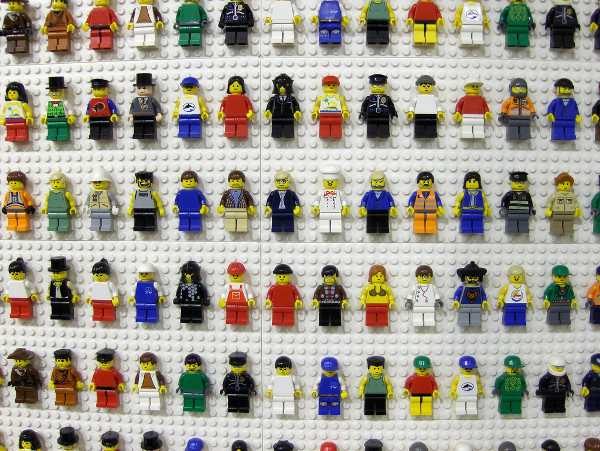
\includegraphics[width=0.95\textwidth]{/part07/lego_people.jpg}
  \begin{center}
    {\large ``Lego People''}\par
    Foto di Joe Shlabotnik\par
    \url{http://www.flickr.com/photos/joeshlabotnik/305410323/}\par
    Licenza: Attribuzione 2.0 Generico (CC BY 2.0)\par
  \end{center}
\clearpage
\cleardoublepage

% (c) 2012 Tiziana Manca - tmanca@libero.it
% (c) 2012 -2014 Dimitrios Vrettos - d.vrettos@gmail.com

\chapter{Statistica descrittiva}

\section{Indagine statistica}
Il termine statistica significa \emph{scienza dello stato}. Questo termine venne usato per la prima volta nel~$XVI$ secolo
per indicare lo studio dei dati utili al governo degli stati prevalentemente relativi a fenomeni di carattere demografico (nascite, morti, ecc.).
Negli anni, la statistica si è estesa ai campi più disparati: fisica, psicologia, ricerca di mercato, indici di gradimento, sondaggi, meteorologia, \ldots
È nata essenzialmente con lo scopo di descrivere i fenomeni (statistica descrittiva), successivamente è divenuta uno strumento utile
anche per fare previsioni (statistica inferenziale). A grandi linee si può definire come la scienza che si occupa della raccolta e dell'analisi dei dati relativi
ad un certo gruppo di persone, animali o oggetti al fine di descrivere in maniera sintetica un fenomeno che li riguarda e fare eventualmente previsioni sul suo andamento futuro.

Ad esempio, la statistica cerca di rispondere a domande del tipo:
\begin{itemize*}
\item quanta acqua sarà necessaria in Italia fra~3 anni?
\item quanta corrente elettrica sarà necessaria per il fabbisogno nazionale fra~5 anni?
\item quale sarà il tasso di disoccupazione nazionale fra~1 anno?
\end{itemize*}

\begin{definizione}
L'insieme di elementi oggetto dell'indagine statistica è detta \emph{popolazione} o universo, mentre ciascun elemento della popolazione è detto \emph{unità statistica}.
\end{definizione}

Sono esempi di popolazione statistica gli abitanti di una città in un certo anno, i prezzi di un determinato bene, le temperature massime registrate
in una giornata in un particolare luogo, i ciclomotori circolanti in Italia, gli alunni di una scuola.

\begin{definizione}
Per ogni unità statistica si possono studiare una o più caratteristiche ed ognuna di tali caratteristiche costituisce un \emph{carattere} della popolazione oggetto
di indagine. I caratteri possono essere di tipo \emph{qualitativo} o \emph{quantitativo}.
Si definisce \emph{modalità} del carattere indagato ciascuno dei diversi modi in cui esso può presentarsi.
\end{definizione}

Sono esempi di carattere qualitativo il colore degli occhi, il colore dei capelli, il tipo di scuola frequentato, il gradimento di un certo programma televisivo.
Le modalità di un carattere qualitativo sono espresse mediante nomi o aggettivi.
I caratteri qualitativi sono a loro volta suddivisi in \emph{ordinabili}, cioè può essere definita una relazione di ordine tra essi (per ogni coppia di elementi si può stabilire quale dei due è il primo e quale il secondo -- es.~il tipo di scuola frequentato è ordinabile a partire dalla scuola dell'infanzia fino alla laurea,
il gradimento di un programma televisivo è ordinabile a partire dalla completa mancanza di gradimento fino al gradimento massimo) e \emph{non ordinabili} o \emph{sconnessi}
(es.~colore degli occhi, colore dei capelli).

Sono invece caratteri quantitativi l'età, l'altezza, il numero di auto prodotte da una fabbrica, \ldots, ovvero le modalità di un carattere quantitativo sono espresse mediante numeri.
I caratteri quantitativi possono essere di tipo \emph{discreto}, quando assumono solo valori puntuali, oppure di tipo \emph{continuo}, quando possono assumere
tutti gli infiniti valori compresi in un determinato intervallo. Sono esempi di caratteri quantitativi discreti il numero di figli in una famiglia,
i pezzi prodotti in una catena di montaggio; sono esempi di caratteri quantitativi continui l'altezza di una persona, il peso di una persona, la lunghezza di un fiume.

L'indagine statistica può riguardare l'intera popolazione (in tal caso si parla di \emph{censimento}) oppure solo una sua parte (in tal caso si parla di \emph{indagine a campione}).
Supponiamo di voler effettuare un'indagine relativa alle persone che fumano in Italia. Il fenomeno collettivo in esame è il fumo, la popolazione di riferimento
è costituita dalla popolazione italiana in età adulta, l'unità statistica è rappresentata da ogni cittadino oggetto dell'indagine, i caratteri oggetto
dell'indagine possono essere ``fumatore/{}non fumatore'', ``numero di sigarette fumate'', che cosa si fuma (es.~ pipa, sigaro, sigaretta). Data l'elevata numerosità
della popolazione di riferimento la tipologia di indagine preferibile è quella a campione.

A sua volta, l'indagine a campione può essere effettuata su un \emph{campione casuale}, quando si scelgono a caso i campioni all'interno della popolazione o
su un \emph{campione stratificato}, quando si suddivide la popolazione in \emph{classi} o \emph{strati} senza specifici criteri e per ogni strato si prende a caso un campione.

\ovalbox{\risolvi \ref{ese:A.1}}

\section{Fasi di un'indagine statistica}
\begin{definizione}
Dato un carattere oggetto di rilevazione, si definisce \emph{frequenza} il numero delle unità statistiche su cui una sua modalità si presenta.
\end{definizione}

Affinché un'indagine statistica sia rigorosa (e quindi garantisca un'elevata affidabilità) è necessario che sia strutturata secondo le seguenti fasi:

\begin{enumeratea}
\item \textbf{Studio del problema e impostazione dell'indagine statistica.}
Si individua in maniera precisa lo scopo della ricerca, il fenomeno sul quale indagare, la popolazione statistica di riferimento,
le singole unità statistiche ed il carattere, o caratteri, oggetto di indagine.
\item \textbf{Rilevazione dei dati statistici.}
La rilevazione non è altro che la raccolta dei dati statistici riguardanti ogni elemento della popolazione e relativi al fenomeno che si vuole analizzare.
La rilevazione può avvenire secondo diverse modalità:
\begin{description}
\item [rilevazione diretta o globale:] viene eseguita direttamente su tutte le unità statistiche che formano la popolazione;
\item [rilevazione indiretta o parziale:] eseguita solo su una parte della popolazione. Si deve scegliere in tal caso un sottoinsieme della popolazione,
detto \emph{campione}, che deve essere rappresentativo della popolazione di riferimento, ovvero deve essere il più possibile eterogeneo rispetto alle caratteristiche della popolazione e contenere al suo interno un numero non troppo ristretto di unità.
\end{description}
\item \textbf{Spoglio delle schede e tabulazione.}
Contemporaneamente o successivamente al rilevamento, i dati raccolti vengono ordinati, suddivisi in classi omogenee e riassunti tramite tabelle dette \emph{tabelle statistiche}.
\item \textbf{Rappresentazione dei dati statistici.}
La rappresentazione può avvenire attraverso diversi tipi di grafico:
\begin{description}
\item [diagramma cartesiano:] rappresentazione nel piano cartesiano dei valori della variabile 	sull'asse orizzontale e delle relative frequenze sull'asse verticale;
\item [ideogramma:] si rappresenta un certo numero di dati con un simbolo;
\item [diagramma a barre o a colonne:] grafico composto da segmenti o barre (orizzontali o verticali) proporzionali alle frequenze;
\item [areogramma:] grafico a forma di cerchio composto da settori circolari con aree direttamente proporzionali alle frequenze;
\item [istogramma:] grafico composto da rettangoli aventi area proporzionale alla frequenza.
\end{description}
\item \textbf{Elaborazione dei dati.}
Con specifici algoritmi di calcolo, vengono elaborati i dati tabulati al fine di costruire opportuni indici di sintesi.
\item \textbf{Interpretazione dei risultati.}
Attraverso i grafici e gli indici è possibile descrivere le caratteristiche peculiari del fenomeno analizzato.
\end{enumeratea}

Analizziamo in dettaglio le singole fasi che seguono la raccolta dei dati.

\subsection{Spoglio delle schede e tabulazione}
Dopo aver raccolto i dati per ciascuna modalità del carattere o per ciascuna classe individuata si deve determinare:

\begin{itemize*}
\item la \emph{frequenza assoluta}, cioè il numero di volte con cui si presenta una modalità del carattere indagato;
\item la \emph{frequenza relativa}, cioè il rapporto tra la frequenza assoluta e il numero totale dei casi presi in esame;
\item la \emph{frequenza percentuale}, cioè la frequenza relativa moltiplicata per~100.
\end{itemize*}
Si compila poi una tabella di frequenza che sintetizza la raccolta dei dati, come nell'esempio seguente.

\begin{exrig}
 \begin{esempio}

La tabella seguente fornisce la distribuzione di frequenze assolute degli alunni di una classe rispetto al carattere sesso.

\begin{center}
\begin{tabular}{lccc}
\toprule
Sesso &Femmine &Maschi &Totale \\
Numero di alunni & 15 & 12 & 27 \\
\bottomrule
\end{tabular}
\end{center}

Per costruirla, si è operata la classificazione della popolazione degli alunni della classe rispetto ad un determinato carattere (il sesso),
sono state individuate le modalità con cui questo si è manifestato (femmina, maschio) ed è stato effettuato il conteggio delle unità
in corrispondenza di ciascuna modalità (frequenza assoluta).
Dalle frequenze assolute si ricavano le frequenze relative:~15 alunni su~27 sono femmine: la frazione è di~$15/27$ femmine sul totale degli alunni. Quindi Dall'operazione~15
diviso~27 otteniamo~$\np{0,56}$ (approssimando a due cifre decimali) che è la frequenza relativa.
La frazione può essere espressa in forma percentuale:~$\np{0,56}$ equivale a dire~56 su~100 ed è consuetudine scriverlo in forma percentuale~$56\%$. Tale valore è la frequenza percentuale.

Ripetendo lo stesso procedimento per i maschi si ottiene la seguente tabella delle frequenze:

\begin{center}
\begin{tabular}{lccc}
\toprule
Sesso & Frequenza assoluta & Frequenza relativa & Frequenza percentuale \\
\midrule
Femmine & 15 & $\np{0,56}$ & $56\%$ \\
Maschi & 12 & $\np{0,44}$ & $44\%$ \\
\bottomrule
\end{tabular}
\end{center}
Si può concludere che la classe è formata per il~$56\%$ da femmine e per il~$44\%$ da maschi.
 \end{esempio}

 \begin{esempio}

Supponiamo che i voti elencati di seguito siano quelli riportati in matematica a fine trimestre
dagli alunni della tua classe: 5, 4, 6, 8, 8, 7, 7, 6, 5, 5, 6, 7.

Per poter effettuare una lettura più agevole si costruisce una tabella in cui vengono riportati sulla prima colonna i singoli valori rilevati (le modalità del carattere) in ordine crescente,
nella seconda la frequenza assoluta, cioè quante volte compare quel determinato voto, nella terza la frequenza relativa e nella quarta quella percentuale (che si ottiene moltiplicando per~100 la frequenza relativa):

\begin{center}
\begin{tabular}{lccc}
\toprule
Voto riportato & Frequenza assoluta & Frequenza relativa & Frequenza percentuale \\
\midrule
4 & 1 & $1/12=\np{0,083}$ & $\np{8,30}\%$ \\
5 & 3 & $3/12=\np{0,25}$ & $\np{25,00}\%$ \\
6 & 3 & $3/12=\np{0,25}$ & $\np{25,00}\%$ \\
7 & 3 & $3/12=\np{0,25}$ & $\np{25,00}\%$ \\
8 & 2 & $2/12=\np{0,167}$ & $\np{16,70}\%$ \\
Totale & 12 & $12/12=1$ & $100\%$ \\
\bottomrule
\end{tabular}
\end{center}
 \end{esempio}

 \begin{esempio}
Misurando l'altezza di un gruppo di cani di razza pastore italiano si sono ottenute le seguenti misure in~$\unit{cm}$:
\begin{center}
 \begin{tabular}{ccccccccccccc}
$\np{57,1}$ & $\np{60,8}$ & $\np{60,7}$ & $\np{56,2}$ & $\np{59,5}$ & $\np{62,4}$ & $\np{56,1}$ & $\np{61,2}$ & $\np{54,5}$ & $\np{64,5}$ & $\np{57,5}$ & $\np{58,3}$ & $\np{55,2}$\\
$\np{58,7}$ & $\np{57,2}$ & $\np{56,1}$ & $\np{58,9}$ & $\np{57,7}$ & $\np{53,2}$ & $\np{59,2}$ & $\np{58,9}$ & $\np{54,5}$ & $\np{55,3}$ & $\np{62,1}$ & $\np{59,0}$ & $\np{58,3}$\\
$\np{61,3}$ & $\np{60,1}$ & $\np{56,4}$ & $\np{60,2}$ & $\np{61,7}$ & $\np{57,3}$ & $\np{58,3}$ & $\np{59,5}$ & $\np{62,6}$ & $\np{59,4}$ & $\np{58,3}$ & $\np{59,4}$ & $\np{59,4}$\\
$\np{59,3}$ & $\np{57,6}$ & $\np{60,0}$ & $\np{60,7}$ & $\np{56,7}$ & $\np{61,1}$	& $\np{59,8}$ & $\np{55,3}$ & $\np{63,9}$ & $\np{58,0}$ & $\np{55,2}$ & $\np{54,9}$ & $\np{53,8}$\\
 \end{tabular}
\end{center}
Il carattere indagato nella popolazione cani pastore italiano è di tipo quantitativo continuo; con questo tipo di dati è praticamente impossibile
calcolare le frequenze se le altezze non si raggruppano in classi.

Vediamo come procedere: osservando i dati ottenuti si nota che il valore minore è~$\np{53,8}$ mentre il valore maggiore è~$\np{64,7}$. Possiamo allora suddividere
i dati in gruppi partendo da~$\np[cm]{53,0}$ fino a~$\np[cm]{65,0}$, formando classi di ampiezza~$1 \unit{cm}$ e ottenendo la seguente tabella:

\begin{center}
\begin{tabularx}{.9\textwidth}{*{2}{lXX}}
\toprule
Classe ($\unit{cm}$) & Frequenza assoluta & Frequenza percent. &Classe ($\unit{cm}$) & Frequenza assoluta & Frequenza percent. \\
\midrule
$\np{53,0}$ - $\np{53,9}$ & 2 & $\np{3,85}\%$ & $\np{59,0}$ - $\np{59,9}$ & 9 & $\np{17,31}\%$\\
$\np{54,0}$ - $\np{54,9}$ & 3 & $\np{5,77}\%$ & $\np{60,0}$ - $\np{60,9}$ & 6 & $\np{11,54}\%$\\
$\np{55,0}$ - $\np{55,9}$ & 4 & $\np{7,69}\%$ & $\np{61,0}$ - $\np{61,9}$ & 4 & $\np{7,69}\%$\\
$\np{56,0}$ - $\np{56,9}$ & 5 & $\np{9,61}\%$ & $\np{62,0}$ - $\np{62,9}$ & 3 & $\np{5,77}\%$\\
$\np{57,0}$ - $\np{57,9}$ & 6 & $\np{11,54}\%$ & $\np{63,0}$ - $\np{63,9}$ & 1 & $\np{1,92}\%$\\
$\np{58,0}$ - $\np{58,9}$ & 8 & $\np{15,38}\%$ & $\np{64,0}$ - $\np{64,9}$ & 1 & $\np{1,92}\%$\\
%\midrule
%Totale & 52 & &&&\\
%\bottomrule
\end{tabularx}
\end{center}

%Nota: vista la natura continua del carattere, la scrittura formalmente più corretta per indicare le classi sarebbe quella degli intervalli chiusi a sinistra e aperti a destra, ad es.~$[53\text{ - }54)$, $[54\text{ - }55)$, \ldots

\end{esempio}
\end{exrig}

\newpage
Riassumendo
\begin{center}
 % (c) 2012 Dimitrios Vrettos - d.vrettos@gmail.com
\begin{tikzpicture}[font=\small,
  punto/.style={%
    draw=RedOrange, 
    rectangle, 
    fill=white,
    very thick, 
    rounded corners,
    text centered,
    text width=35mm,
    minimum height=1.5em},
  subpunto/.style={%
    draw=RedOrange, 
    rectangle, 
    fill=white,
    very thick, 
    rounded corners,
    text centered,
    text width=44mm,
    minimum height=4em},
  subpunto1/.style={%
    draw=RedOrange, 
    rectangle, 
    fill=white,
    very thick, 
    rounded corners,
    text centered,
    text width=15mm,
    minimum height=1.5em},
  level distance=15mm,
  level 3/.style={sibling distance=50mm},
  level 4/.style={sibling distance=25mm}, 
  edge from parent/.style={draw,->,OliveGreen, thick, shorten >=2pt}]
  
\node [punto] {Popolazione Universo}
  child {node [punto] {Unit\`a statistiche}
    child {node [punto]{Caratteri \\delle unit\`a statistiche}
      child{node [subpunto]{Caratteri di tipo qualitativo \\Modalit\`a non numeriche \\Aggettivi, nomi, professioni}
	child {node [subpunto1]{ordinabili}}
	child {node [subpunto1]{sconnessi}}}
      child {node [subpunto]{Caratteri di tipo quantitativo \\Modalit\`a numeriche \\Intensit\`a o classi d'intensit\`a}
	child {node[subpunto1] {continuo}}
	child {node[subpunto1] {discreto}}}}};
\end{tikzpicture}

\end{center}

\ovalbox{\risolvii \ref{ese:A.2}, \ref{ese:A.3}, \ref{ese:A.5}, \ref{ese:A.6}, \ref{ese:A.7}, \ref{ese:A.8}, \ref{ese:A.9}}

\subsection{Rappresentazione grafica}

La rappresentazione grafica dei dati statistici facilita notevolmente lo studio delle caratteristiche del
fenomeno che si sta esaminando; infatti dopo aver impostato l'indagine, raccolto, classificato ed elaborato i dati nelle tabelle,
i dati non sempre si presentano in una forma di facile lettura ed il loro significato e la loro interpretazione rimane poco chiara.
Attraverso la rappresentazione grafica, i risultati dell'indagine emergono immediatamente, in maniera diretta e sintetica.

La rappresentazione grafica può avvenire utilizzando diversi tipi di grafico a seconda delle caratteristiche da
analizzare.

\subsubsection{Diagramma cartesiano}
La rappresentazione grafica attraverso un diagramma cartesiano dà, in modo immediato, informazioni sull'andamento globale del fenomeno e viene
utilizzata prevalentemente per la rappresentazione di serie storiche (per esempio, per rappresentare il numero di auto prodotte per anno da una fabbrica)
oppure quando si hanno due caratteri quantitativi e si vuol analizzare il tipo di legame esistente fra di essi.


\begin{exrig}
 \begin{esempio}

Consideriamo la tabella statistica relativa alla domanda ``quante ore al giorno passi al computer?'', posta ad un
campione di~50 ragazzi dai~16 ai~24 anni.

Rappresentiamo la tabella attraverso un diagramma cartesiano costruito tracciando due rette perpendicolari, gli assi, quello verticale orientato verso
l'alto e quello orizzontale orientato verso destra. Riportiamo sull'asse orizzontale il numero di ore e sull'asse verticale il numero di ragazzi e determiniamo
i punti aventi come coordinate (numero ore; numero ragazzi).

Il punto~$A$ avrà come coordinate~$(0;4)$, il punto~$B$ avrà come coordinate~$(1;6)$ e così via. Uniamo poi
i punti con segmenti e otteniamo il diagramma cartesiano~(grafico~\ref{gr:A.1}).
Precisamente~$A(0;4)$, $B(1;6)$, $C(2;12)$, $D(3;16)$, $E(4;8)$, $F(5;4)$, $G(6;2)$.

\begin{center}
\begin{tabular}{lccccccc}
\toprule
Numero di ore & 0 & 1 &2 & 3 & 4 & 5 & 6\\
Numero di ragazzi & 4 & 6 & 12 & 16 & 8 & 4 & 2 \\
\bottomrule
\end{tabular}
\end{center}
Dal grafico~\ref{gr:A.2} si può notare immediatamente che la maggior parte dei ragazzi trascorre dalle~2 alle~3 ore al computer dato che il picco più
alto si ha proprio nei punti~$C$ e~$D$.
Si può anche notare che, ad esempio, il punto~$X$ di coordinate~$(\np{3,5};12)$, appartenente al segmento di congiunzione tra i punti~$D$ ed~$E$,
non ha significato reale, dato che le sue coordinate non sono riportate nella tabella statistica del fenomeno da studiare.
\begin{grafico}[t]
\begin{minipage}{0.5\textwidth}
% (c) 2012 Dimitrios Vrettos - d.vrettos@gmail.com
\begin{tikzpicture}[scale=.75]
  \tikzset{
    every pin/.style={pin distance=0,font=\small},
  }

\begin{axis}[xlabel=$n\grado$ ore, ylabel=$n\grado$ ragazzi,xmin=0]
  \addplot[color=blue, mark=*]
    coordinates{
      (0,4) 
      (1,6)
      (2,12)
      (3,16)
      (4,8)
      (5,4)
      (6,2)
      };

  \node[pin=0:{$A(0;4)$}] at (axis cs:0,4) {};
  \node[pin=0:{$B(1;6)$}] at (axis cs:1,6) {};
  \node[pin=180:{$C(2;12)$}] at (axis cs:2,12) {};
  \node[pin=0:{$D(3;16)$}] at (axis cs:3,16) {};
  \node[pin=0:{$E(4;8)$}] at (axis cs:4,8) {};
  \node[pin=0:{$F(5;4)$}] at (axis cs:5,4) {};
   \node[pin=180:{$G(6;2)$}] at (axis cs:6,2) {};
\end {axis}
\end{tikzpicture}

\caption{Esempio~24.4}\label{gr:A.1}
\end{minipage}\hfill
\begin{minipage}{0.5\textwidth}
% (c) 2012 Dimitrios Vrettos - d.vrettos@gmail.com
\begin{tikzpicture}[scale=.75]
  \tikzset{
    every pin/.style={pin distance=0,font=\small},
  }

  \begin{axis}[xlabel=$n\grado$ ore, ylabel=$n\grado$ ragazzi,xmin=0]
    \addplot[only marks, color=blue, mark=*]
      coordinates{
	(0,4) 
	(1,6)
	(2,12)
	(5,4)
	(6,2)
      };
 \addplot[color=grigio70, mark=*]
      coordinates{
	(0,4)
	(1,6)
	(2,12)
   (3,16)
      };    
 \addplot[color=grigio70, mark=*]
      coordinates{
	(6,2)
	(5,4)
	(4,8)
      };
 \addplot[color=blue, mark=*]
      coordinates{
	(3,16)
	(4,8)
      };
 \addplot[color=red, mark=*]
      coordinates{
	(3.5,12)
      };

    \node[pin=0:{$A(0;4)$}] at (axis cs:0,4) {};
    \node[pin=0:{$B(1;6)$}] at (axis cs:1,6) {};
    \node[pin=180:{$C(2;12)$}] at (axis cs:2,12) {};
    \node[pin=0:{$D(3;16)$}] at (axis cs:3,16) {};
    \node[pin=0:{$E(4;8)$}] at (axis cs:4,8) {};
    \node[pin=0:{$F(5;4)$}] at (axis cs:5,4) {};
    \node[pin=180:{$G(6;2)$}] at (axis cs:6,2) {};
    \node[pin=0:{$X(3,5;12)$}] at (axis cs:3.5,12) {};
  \end {axis}
\end{tikzpicture}

\caption{Esempio~24.4}\label{gr:A.2}
\end{minipage}
\end{grafico}
\end{esempio}
\end{exrig}

\subsubsection{Ideogramma}
Nella rappresentazione grafica attraverso \emph{ideogramma} si rappresenta un certo numero di dati con un simbolo che si assume come \emph{unità grafica};
il simbolo deve richiamare l'oggetto dell'indagine e dare quindi una visione immediata del fenomeno.
Ad esempio si può utilizzare un uomo stilizzato per rappresentare un dato riguardante il numero di persone che vivono in un determinato territorio,
una macchina per la produzione annua di automobili in una fabbrica, e così via.
Tale tipo di rappresentazione è spesso usata in campo pubblicitario perché caratterizzata da un evidente impatto visivo.

\begin{exrig}
 \begin{esempio}

Un istituto scolastico ha visto aumentare i suoi iscritti, dall'anno scolastico~2003-2004 all'anno~2008-2009 secondo quanto riportato nella seguente tabella:

\begin{center}
 \begin{tabular}{lcccccc}
 \toprule
 Anno scolastico & 2003-04 & 2004-05 & 2005-06 & 2006-07 & 2007-08 & 2008-09\\
 Iscritti & 150 & 200 & 200 & 325 & 375 & 450\\
 \bottomrule
\end{tabular}
\end{center}

Possiamo rappresentare mediante ideogramma i dati contenuti nella tabella statistica.
Consideriamo una faccina stilizzata come unità grafica assegnandole il valore di~50 ragazzi iscritti.
\begin{center}
 % (c) 2012 Dimitrios Vrettos - d.vrettos@gmail.com

\begin{tikzpicture}
\begin{scope}[RedOrange]
\draw(0,-.5ex) circle (1.5ex);
\foreach \x in {-.5ex,.5ex}
  \draw[fill=white] (\x,0) circle (.2ex);
   \draw (-.9ex,-1ex)..controls (-0.4ex,-1.5ex)and(0.5ex,-1.5ex)..(.9ex,-1ex);
\end{scope}
\node () at (8ex,-.5ex) { $=$ 50 iscritti};
\end{tikzpicture}

\end{center}
Il numero degli iscritti di ogni anno scolastico sarà rappresentato da tante unità grafiche quanti sono i gruppi di~50 iscritti.
Per avere il grafico relativo all'anno~2003-2004 si devono usare tre faccine, in quanto~$150:50=3$.
\begin{center}
 \begin{tikzpicture}
\begin{scope}[RedOrange]
\foreach \xi in {0,3.5ex,7ex}{
\draw(\xi,-.5ex) circle (1.5ex);
   \draw (\xi-.9ex,-1ex)..controls (\xi-0.4ex,-1.5ex)and(\xi+0.5ex,-1.5ex)..(\xi+.9ex,-1ex);}
\foreach \xii in {-.5ex,.5ex,3ex,4ex,6.5ex,7.5ex}
  \draw[fill=white] (\xii,0) circle (.2ex);
\end{scope}
\node[left] at (-1.5ex,-.5ex) { a.s. 2003-2004 $=$};
\end{tikzpicture}

\end{center}
Se la divisione del numero degli iscritti per~50 dà resto, esso si dovrà rappresentare disegnando solo una parte
dell'unità grafica, corrispondente alla frazione tra resto e~50. Ad esempio nell'~a.s.~2006-2007 ci sono stati~325 iscritti; $325:50 = 6$
col resto di~25, quindi~325 sarà uguale a~6 unità grafiche e~$\frac{25}{50}=\frac{1}{2}$ unità grafica, cioè mezza faccina, ovvero $325:50 = \np{6,5}$ cioè 6 faccine e mezzo.
\begin{center}
 % (c) 2012 Dimitrios Vrettos - d.vrettos@gmail.com

\begin{tikzpicture}
\begin{scope}[RedOrange]
\foreach \xi in {0,3.5ex,7ex,10.5ex,14ex,17.5ex,21ex}{
\draw(\xi,-.5ex) circle (1.5ex);
   \draw (\xi-.9ex,-1ex)..controls (\xi-0.4ex,-1.5ex)and(\xi+0.5ex,-1.5ex)..(\xi+.9ex,-1ex);}
\foreach \xii in {-.5ex,.5ex,3ex,4ex,6.5ex,7.5ex,10ex,11ex,13.5ex,14.5ex,17ex,18ex,20.5ex,21.5ex}
  \draw[fill=white] (\xii,0) circle (.2ex);
\end{scope}
\filldraw[white] (21ex,-2.2ex) rectangle (23ex,1.2ex);
\node[left] at (-1.5ex,-.5ex) { a.s. 2006-2007 $=$};
\end{tikzpicture}

\end{center}

Il grafico completo sarà:
\begin{center}
 % (c) 2012 Dimitrios Vrettos - d.vrettos@gmail.com

\begin{tikzpicture}[RedOrange]
  \foreach \xi in {0,3.5ex,7ex}{
    \draw(\xi,-.5ex) circle (1.5ex);
    \draw (\xi-.9ex,-1ex)..controls (\xi-0.4ex,-1.5ex)and(\xi+0.5ex,-1.5ex)..(\xi+.9ex,-1ex);
  }
  \foreach \xii in {-.5ex,.5ex,3ex,4ex,6.5ex,7.5ex}
    \draw[fill=white] (\xii,0) circle (.2ex);
  
  \node[left,black] at (-1.5ex,-.5ex) { a.s. 2003-2004 $=$};
  \node[right,black] at(30ex,-.5ex){3};

  \begin{scope}[yshift=-4ex]
    \foreach \xi in {0,3.5ex,7ex,10.5ex}{
      \draw(\xi,-.5ex) circle (1.5ex);
      \draw (\xi-.9ex,-1ex)..controls (\xi-0.4ex,-1.5ex)and(\xi+0.5ex,-1.5ex)..(\xi+.9ex,-1ex);
    }
    \foreach \xii in {-.5ex,.5ex,3ex,4ex,6.5ex,7.5ex,10ex,11ex}
      \draw[fill=white] (\xii,0) circle (.2ex);
    \node[left,black] at (-1.5ex,-.5ex) { a.s. 2004-2005 $=$};
    \node[right,black] at(30ex,-.5ex){4};
  \end{scope}

  \begin{scope}[yshift=-8ex]
    \foreach \xi in {0,3.5ex,7ex,10.5ex}{
      \draw(\xi,-.5ex) circle (1.5ex);
      \draw (\xi-.9ex,-1ex)..controls (\xi-0.4ex,-1.5ex)and(\xi+0.5ex,-1.5ex)..(\xi+.9ex,-1ex);}
    \foreach \xii in {-.5ex,.5ex,3ex,4ex,6.5ex,7.5ex,10ex,11ex}
      \draw[fill=white] (\xii,0) circle (.2ex);
    \node[left,black] at (-1.5ex,-.5ex) { a.s. 2005-2006 $=$};
    \node[right,black] at(30ex,-.5ex){4};
  \end{scope}

  \begin{scope}[yshift=-12ex]
    \foreach \xi in {0,3.5ex,7ex,10.5ex,14ex,17.5ex,21ex}{
      \draw(\xi,-.5ex) circle (1.5ex);
      \draw (\xi-.9ex,-1ex)..controls (\xi-0.4ex,-1.5ex)and(\xi+0.5ex,-1.5ex)..(\xi+.9ex,-1ex);}
    \foreach \xii in {-.5ex,.5ex,3ex,4ex,6.5ex,7.5ex,10ex,11ex,13.5ex,14.5ex,17ex,18ex,20.5ex,21.5ex}
      \draw[fill=white] (\xii,0) circle (.2ex);
    \node[left, black] at (-1.5ex,-.5ex) { a.s. 2006-2007 $=$};\filldraw[white] (21ex,-2.2ex) rectangle (23ex,1.2ex);
    \node[right,black] at(30ex,-.5ex){6 e  1/2};
  \end{scope}

  \begin{scope}[yshift=-16ex]
    \foreach \xi in {0,3.5ex,7ex,10.5ex,14ex,17.5ex,21ex,24.5ex}{
      \draw(\xi,-.5ex) circle (1.5ex);
      \draw (\xi-.9ex,-1ex)..controls (\xi-0.4ex,-1.5ex)and(\xi+0.5ex,-1.5ex)..(\xi+.9ex,-1ex);}
    \foreach \xii in {-.5ex,.5ex,3ex,4ex,6.5ex,7.5ex,10ex,11ex,13.5ex,14.5ex,17ex,18ex,20.5ex,21.5ex,24ex,25ex}
      \draw[fill=white] (\xii,0) circle (.2ex);
    \node[left, black] at (-1.5ex,-.5ex) { a.s. 2007-2008 $=$};\filldraw[white] (24.5ex,-2.2ex) rectangle (26.5ex,1.2ex);
    \node[right,black] at(30ex,-.5ex){7 e  1/2};
  \end{scope}

  \begin{scope}[yshift=-20ex]
    \foreach \xi in {0,3.5ex,7ex,10.5ex,14ex,17.5ex,21ex,24.5ex,28ex}{
      \draw(\xi,-.5ex) circle (1.5ex);
      \draw (\xi-.9ex,-1ex)..controls (\xi-0.4ex,-1.5ex)and(\xi+0.5ex,-1.5ex)..(\xi+.9ex,-1ex);}
    \foreach \xii in {-.5ex,.5ex,3ex,4ex,6.5ex,7.5ex,10ex,11ex,13.5ex,14.5ex,17ex,18ex,20.5ex,21.5ex,24ex,25ex,27.5ex,28.5ex}
      \draw[fill=white] (\xii,0) circle (.2ex);
    \node[left, black] at (-1.5ex,-.5ex) { a.s. 2008-2009 $=$};
    \node[right,black] at(30ex,-.5ex){9};
    \end{scope}
\end{tikzpicture}

\end{center}
 \end{esempio}
\end{exrig}

\subsubsection{Diagramma a barre o a colonne}

Questo tipo di rappresentazione, detta anche diagramma a nastri o a bastoni, viene usata quando si vuole fornire un'idea delle frequenze
delle diverse modalità di un fenomeno. In genere si usa per caratteri qualitativi o quantitativi discreti.
Per poter valutare il significato statistico della lunghezza delle barre (o delle colonne) è necessario scegliere opportunamente una scala di riferimento:
la larghezza della barra (o della colonna) è arbitraria ma uguale per tutte le barre (o colonne) e la sua lunghezza è proporzionale alla caratteristica che si deve rappresentare.
Le barre (o le colonne) possono inoltre essere suddivise in parti di colori diversi per indicare le singole componenti o i singoli fenomeni
che si vogliono analizzare.

La differenza fra la rappresentazione a barre e quella a colonne consiste soltanto
nell'orientamento del grafico: nel diagramma a barre si indicano le modalità del carattere sull'asse verticale e le frequenze sull'asse orizzontale,
mentre in quello a colonne le modalità del carattere sono riportate sull'asse
orizzontale e le frequenze su quello verticale.

Di seguito vengono riportate le due tipologie di grafico accompagnate dalla tabella di riferimento:
\begin{center}
 \begin{tabularx}{.95\textwidth}{X*{7}{c}Xc}
\toprule
Materia& Italiano &Storia & Geografia & Matem. & Scienze & Ed. Fisica & Totale\\
Maschi & 5 & 4& 4 & 2& 6 & 5& 26\\
Femmine & 3 & 7 & 2 & 3  & 4 & 5 & 24\\
\bottomrule
\end{tabularx}
\end{center}

\begin{center}
\begin{figure}[!ht]
% (c) 2012 Dimitrios Vrettos - d.vrettos@gmail.com

\begin{tikzpicture}
\begin{axis}[
legend entries={Maschi, Femmine},
legend pos=outer north east,
xbar,
enlarge y limits=0.15,
symbolic y coords={Educaz. fisica,Scienze,Matematica, Geografia,Storia,Italiano },
ytick=data,
bar width=8pt, 
xmin=0, 
width=100mm]

\addplot[fill=CornflowerBlue, draw=black] coordinates {
(5,Educaz. fisica)
(6,Scienze)
(2,Matematica)
(4,Geografia)
(4,Storia)
(5,Italiano)
};

\addplot[fill=pink, draw=black] coordinates{
(5,Educaz. fisica)
(4,Scienze)
(3,Matematica)
(2,Geografia)
(7,Storia)
(3,Italiano)
};
\end{axis}
\end{tikzpicture}

\caption{Diagramma a barre}
\end{figure}
\end{center}

\begin{center}
 \begin{figure}[!ht]
% (c) 2012 Dimitrios Vrettos - d.vrettos@gmail.com

\begin{tikzpicture}
\begin{axis}[
legend entries={Maschi, Femmine},
legend pos=outer north east,
ybar,
enlarge x limits=0.15,
symbolic x coords={E. F.,Scienze,Matem., Geografia,Storia,Italiano },
xtick=data,
bar width=15pt, 
ymin=0, 
width=110mm]

\addplot[fill=CornflowerBlue, draw=black] coordinates {
(E. F.,5)
(Scienze,6)
(Matem.,2)
(Geografia,4)
(Storia,4)
(Italiano,5)
};
 
 \addplot[fill=pink, draw=black] coordinates{
 (E. F.,5)
 (Scienze,4)
 (Matem.,3)
 (Geografia,2)
 (Storia,7)
 (Italiano,3)
 };
\end{axis}
\end{tikzpicture}

\caption{Diagramma a colonne}
\end{figure}
\end{center}

\subsubsection{Areogramma}

Questo tipo di rappresentazione, detta anche grafico a torta, viene utilizzato quando si vogliono evidenziare le parti che compongono un fenomeno, per esempio per indicare
come si dividono gli alunni di una classe in maschi e femmine, o per rappresentare in che modo
le varie voci di spesa incidono sul bilancio familiare.
Il grafico si ottiene dividendo un cerchio in settori circolari con aree direttamente proporzionali alle frequenze che rappresentano.
Per disegnare l'areogramma, si disegna una circonferenza di diametro arbitrario e si fa corrispondere l'angolo al centro di~$360\grado$,
con il~$100\%$ di frequenza percentuale; per ottenere l'angolo corrispondente ad una certa frequenza percentuale $f_x$ si risolve la proporzione~$360\grado:X\grado=100:f_x\:\Rightarrow\:X\grado = \np{3,6} \cdot f_x$.
Si suddivide così la circonferenza negli angoli ottenuti e si evidenziano in maniera differente tra loro i settori circolari ottenuti.

\begin{exrig}
 \begin{esempio}
Consideriamo la seguente tabella statistica che indica gli studenti di un dato istituto scolastico divisi per classe frequentata, in un dato anno.

\begin{center}
\begin{tabular}{lcccccc}
\toprule
Classe & 1\textsuperscript{a} &2\textsuperscript{a} &3\textsuperscript{a} & 4\textsuperscript{a} &5\textsuperscript{a} &Totale\\
Studenti & 320 & 230 & 212 & 152 & 96 & $\np{1010}$ \\
\bottomrule
\end{tabular}
\end{center}

Nella tabella sono indicate le frequenze assolute; calcoliamo ora le frequenze percentuali degli studenti.
Per la~1\textsuperscript{a} classe si ha:~$\frac{320}{\np{1010}}=\np{0,32}$ arrotondato alla seconda cifra decimale, che equivale al~$32\%$ e così via per le classi successive.

\begin{center}
\begin{tabular}{lcccccc}
\toprule
Classe & 1\textsuperscript{a} & 2\textsuperscript{a} & 3\textsuperscript{a} & 4\textsuperscript{a} & 5\textsuperscript{a} & Totale \\
 Frequenze percentuali& $32\%$ & $23\%$ & $21\%$ & $15\%$ & $9\%$ & $100\%$ \\
\bottomrule
\end{tabular}
\end{center}

Rappresentiamo graficamente mediante areogramma i dati contenuti nella tabella precedente.
\begin{center}
 \begin{tikzpicture}[x=10mm,y=10mm, x radius=10mm, y radius=10mm]
  \draw (0,0) circle (3);
  \draw[pattern=north east lines,pattern color=orange] (0,0) -- (0:3) arc (0:115.2:3);
  \draw[pattern=horizontal lines,pattern color=brown] (0,0)-- (115.2:3) arc (115.2:198:3);
  \draw[pattern=dots,pattern color=green] (0,0)-- (198:3) arc (198:273.6:3);
  \draw[pattern=north west lines,pattern color=red] (0,0)-- (273.6:3) arc (273.6:327.6:3);
  \draw[pattern=vertical lines,pattern color=blue] (0,0)-- (327.6:3) arc (327.6:360:3);

  \begin{scope}[every node/.style={rounded corners, draw=black, fill=white}]
    \draw(57.6:2) node {$115,2\grado $};
    \draw(156.6:2) node {$82,8\grado $};
    \draw(235.8:2) node {$75,6\grado $};
    \draw(300.6:2) node {$54\grado $};
    \draw(343.8:2) node {$32,4\grado $};
  \end{scope}

  \begin{scope}[thin, <->]
    \draw (0:1) arc (0:115.2:1);
    \draw (115.2:.8) arc (115.2:198:.8);
    \draw (198:1.2) arc (198:273.6:1.2);
    \draw (273.6:.8) arc (273.6:327.6:.8);
    \draw (327.6:1.1) arc (327.6:360:1.1);
  \end{scope}

  \draw(57.6:4) node {1\textsuperscript{a} classe: $32\%$};
  \draw[left](156.3:3) node {2\textsuperscript{a} classe: $23\%$};
  \draw(235.8:4) node {3\textsuperscript{a} classe: $21\%$};
  \draw[below right](300.6:3) node {4\textsuperscript{a} classe: $15\%$};
  \draw[right](343.8:3) node {5\textsuperscript{a} classe: $9\%$};
\end{tikzpicture}

\end{center}

Per ottenere l'angolo relativo alla frequenza percentuale della~1\textsuperscript{a} classe si fa:~$\np{3,6} \cdot 32=\np{115,2}\grado$ e
per la~2\textsuperscript{a} classe:~$\np{3,6} \cdot 23=\np{82,2}\grado$ e così via per le altre classi.

Dal grafico si può notare immediatamente che la classe più frequentata è la prima.

 \end{esempio}
\end{exrig}

\subsubsection{Istogramma}

Si utilizza la rappresentazione grafica attraverso istogramma quando il carattere analizzato è di tipo quantitativo ed i dati sono raggruppati in classi.

Prima di tutto si distribuiscono i dati in classi o gruppi e si determina il numero di unità appartenenti a ciascuna classe; questo numero è
detto \emph{frequenza della classe}.
Riportando tali dati in una tabella si ottiene la distribuzione delle frequenze. Poiché le classi potrebbero avere ampiezze diverse si calcola
la \emph{densità di frequenza}, definita come il rapporto fra la frequenza della classe e la relativa ampiezza.

Per disegnare un istogramma si tracciano due assi; sull'asse verticale, orientato verso l'alto, si fissa un segmento unitario e vi si riportano
le densità di frequenza. L'asse orizzontale, orientato verso destra, è invece suddiviso in tanti segmenti la cui ampiezza è pari a quella delle singole classi.
Il grafico consiste in un insieme di rettangoli aventi per base ogni classe e altezza la densità di frequenza corrispondente.
In tal modo l'area di ogni rettangolo rappresenta la frequenza corrispondente a ciascuna classe.

\begin{exrig}
 \begin{esempio}

Costruiamo un istogramma a partire dalla distribuzione di frequenza riportata nella seguente tabella:
\begin{center}
\begin{tabular}{cc}
\toprule
Diametro crateri lunari ($\unit{km}$) & Numero di crateri\\
\midrule
$0-50$ & $\np{1088}$ \\
$50-100$ & $745$ \\
$100-150$ & $20$ \\
\bottomrule
\end{tabular}
\end{center}

Innanzi tutto per ogni classe dobbiamo determinare la densità di frequenza, che si ottiene dividendo la frequenza assoluta per l'ampiezza della classe:

\begin{center}
\begin{tabular}{cc}
\toprule
Diametro crateri lunari ($\unit{km}$) & Densità di freq.\\
\midrule
$0-50$ & $\np{1088}/50=\np{21,76}$ \\
$50-100$ & $745/50=\np{14,9}$ \\
$100-150$ & $20/50=\np{0,4}$ \\
\bottomrule
\end{tabular}
\end{center}

\begin{center}
% (c) 2012 Dimitrios Vrettos - d.vrettos@gmail.com

\begin{tikzpicture}[scale=.85]
\begin{axis}[
xlabel=Diametro crateri lunari (km), ylabel=Densità di frequenza,
legend entries={Frequenza crateri},
ybar,
enlarge x limits=0.15,
symbolic x coords={$0-50$,$50-100$,$100-150$},
xtick=data,
bar width=30pt, 
ymin=0, 
width=90mm]

\addplot[fill=CornflowerBlue, draw=black] coordinates {
($0-50$,21.76)
($50-100$,14.9)
($100-150$,.4)
 };
 
\end{axis}
\end{tikzpicture}

\end{center}
\end{esempio}

\begin{esempio}
Consideriamo la seguente tabella statistica che riporta i giorni di pioggia di ogni mese, in un dato anno e in una data città.

\begin{center}
\begin{tabular}{lclc}
\toprule
Mesi & Giorni di pioggia &Mesi & Giorni di pioggia\\
\midrule
Gennaio & 15&Luglio & 1 \\
Febbraio & 10 &Agosto & 3\\
Marzo & 14 &Settembre & 3\\
Aprile & 8 &Ottobre & 5\\
Maggio & 5 &Novembre & 9\\
Giugno & 2 &Dicembre & 11\\
\bottomrule
\end{tabular}
\end{center}
Dividiamo i mesi dell'anno in classi, raggruppandoli in stagioni. Ad esempio, Luglio, Agosto e Settembre
appartengono alla classe dell'Estate e la frequenza di questa classe è data dalla somma delle frequenze di ogni mese, cioè~$1 + 3 + 3 = 7$. Si prosegue in questo modo per ogni classe ottenendo così la distribuzione delle frequenze riportata nella tabella.
\begin{center}
\begin{tabular}{lcccc}
\toprule
Stagioni & Estate & Autunno & Inverno& Primavera\\
Giorni di pioggia & 7 & 25 & 39 & 15 \\
\bottomrule
\end{tabular}
\end{center}
Costruisci ora l'istogramma corrispondente alla tabella precedente riportando sull'asse orizzontale le classi (stagioni) e su quello verticale le densità di frequenze.
 \end{esempio}
\end{exrig}

\ovalbox{\risolvii \ref{ese:A.10}, \ref{ese:A.11}, \ref{ese:A.12}, \ref{ese:A.13}, \ref{ese:A.14}, \ref{ese:A.15}, \ref{ese:A.16}, \ref{ese:A.17}, \ref{ese:A.18}, \ref{ese:A.19}, \ref{ese:A.20}}

\section{Indici di posizione}

Nel caso in cui il carattere considerato nell'indagine sia di tipo quantitativo, l'andamento dei dati raccolti può essere sinteticamente descritto per mezzo di opportuni indici. Gli \emph{indici di posizione} vengono utilizzati per dare un'indicazione sulla distribuzione delle frequenze per mezzo di un solo numero.
A seconda del carattere oggetto dell'indagine statistica possono essere utilizzati indici differenti.

\subsection{Moda}

\begin{definizione}
La \emph{moda} è la modalità del carattere indagato che si presenta più frequentemente.
\end{definizione}

In una successione di~$n$ modalità~$x_1$, $x_2$, \ldots, $x_n$
con le relative frequenze~$f_1$, $f_2$, \ldots, $f_n$, la moda è la modalità che ha la frequenza maggiore.
Questo valore può essere calcolato per qualunque tipo di carattere, sia qualitativo che quantitativo.
Se il carattere è quantitativo continuo con dati raggruppati in classi non è possibile determinare con esattezza la moda, ci si limita
ad individuare la \emph{classe modale} definita come la classe cui è associata la massima densità di frequenza.

\begin{exrig}
 \begin{esempio}

 Nella tabella seguente sono riportati i numeri degli studenti, divisi per classe, della sezione~A di un dato istituto,
 in un dato anno. Si può osservare che la~1\textsuperscript{a} classe presenta la frequenza massima di~320 studenti, quindi la moda è la classe prima.
\begin{center}
\begin{tabular}{lcccccc}
\toprule
Classe & 1$\grado$ & 2$\grado$ & 3$\grado$ & 4$\grado$ & 5$\grado$ & Totale \\
Studenti & 320 & 230 & 212 & 152 & 96 & 1\,010 \\
\bottomrule
\end{tabular}
\end{center}
 \end{esempio}

\begin{esempio}
La tabella raccoglie i dati relativi alla domanda ``quante ore alla settimana pratichi sport?'', posta ad un
campione di~50 ragazzi dai~18 ai~25 anni. Si può osservare che~12 e~18 ore presentano la frequenza massima~14, quindi si hanno due
mode~12 ore e~18 ore. In questo caso la distribuzione è bimodale.


\begin{center}
\begin{tabular}{lcccccccc}
\toprule
Numero di ore & 0 &4 &8 &12 &16 &18 &22 &Totale\\
 Numero di ragazzi& 4 & 1 & 3 & 14 & 8 & 14 & 6 & 50 \\
\bottomrule
\end{tabular}
\end{center}
 \end{esempio}

 \begin{esempio}
La tabella seguente è relativa alla distribuzione delle classi di altezza di un gruppo di studenti.

\begin{center}
\begin{tabular}{lcccccc}
\toprule
Altezza (cm) &160-165 &165-170 &170-175 &175-185 &185-200 &Totale \\
Numero di studenti & 5 & 8 & 15 & 10 & 2 & 40 \\
\bottomrule
\end{tabular}
\end{center}
Poiché le classi hanno ampiezza diversa è necessario calcolare la densità di frequenza.

\begin{center}
\begin{tabular}{lccccc}
\toprule
Altezza &160-165 &165-170 &170-175 &175-185 &185-200 \\
Densità di frequenza & 1 & $\np{1,6}$ & 3 & 1 & $\np{0,13}$ \\
\bottomrule
\end{tabular}
\end{center}
La massima densità di frequenza si ha in corrispondenza della classe~170-175, essa rappresenta quindi la classe modale.
 \end{esempio}
\end{exrig}

\subsection{Media aritmetica}

\begin{definizione}
La \emph{media aritmetica} (semplice) è il valore ottenuto sommando tutti i dati e
dividendo tale somma per il numero dei dati.
\end{definizione}

Se abbiamo~$n$ dati~$x_1$, $x_2$, \ldots, $x_n$, la media aritmetica semplice~$M$ è data da:

\begin{equation*}
M=\frac{x_1+x_2+ \dots +x_n}{n}=\frac{1}{n}\sum_{i=1}^n x_i.
\end{equation*}

\begin{exrig}
 \begin{esempio}

Riprendiamo in esame la tabella relativa agli studenti, divisi per classe frequentata di un dato istituto scolastico, in un dato anno e calcoliamone la media aritmetica semplice.
\begin{center}
 \begin{tabular}{lcccccc}
 \toprule
 Classe & 1\textsuperscript{a} & 2\textsuperscript{a} & 3\textsuperscript{a} & 4\textsuperscript{a} & 5\textsuperscript{a} & Totale\\
 Studenti & 320 & 230 & 212 & 152 & 96 & $\np{1010}$\\
 \bottomrule
\end{tabular}
\end{center}
Per calcolare la media aritmetica semplice degli studenti, sommiamo tutti gli studenti delle cinque classi e dividiamo tale somma per il numero delle classi:
\begin{equation*}
M=\frac{320+230+212+152+96}{5}= \frac{\np{1010}}{5}= 202.
\end{equation*}
Possiamo dire che si hanno mediamente~202 studenti per ogni classe.

\begin{definizione}
Si definisce \emph{scarto dalla media} (aritmetica) la differenza tra i valori osservati e la media.
\end{definizione}

Se~$x_1$, $x_2$, \ldots, $x_n$ sono i valori osservati e $M$ la loro media aritmetica, gli scarti sono~$s_1=x_1-M$, $s_2=x_2-M$, \ldots, $s_n=x_n-M$.
\end{esempio}

\begin{esempio}
Calcoliamo gli scarti dalla media per la distribuzione ``studenti per tipologia di classe frequentata'', la cui media è~$\np{1010}/5 = 202$.
\begin{center}
\begin{tabular}{l*{6}{c}}
\toprule
Classe & 1\textsuperscript{a} & 2\textsuperscript{a} & 3\textsuperscript{a} & 4\textsuperscript{a} & 5\textsuperscript{a} & Totale\\
Studenti & 320& 230& 212& 152& 96& $\np{1010}$ \\
Scarto & 118 & 28 & 10 & $-50$ & 106 & 0\\
\bottomrule
\end{tabular}
\end{center}
Si può osservare che vi solo valori superiori alla media e altri inferiori, tanto che lo scarto è rappresentato in
alcuni casi da un numero positivo, in altri da un numero negativo. Si può verificare che la somma degli scarti dalla media è nulla,
cioè gli scarti positivi compensano sempre quelli negativi.
 \end{esempio}
\end{exrig}


\begin{definizione}
La \emph{media aritmetica ponderata} è il valore ottenuto moltiplicando ciascuna modalità del carattere
dato con la propria frequenza, sommando tutti i prodotti fra loro e dividendo poi per la somma delle frequenze
(che equivale al numero totale $n$ delle unità statistiche considerate).
\end{definizione}

La media aritmetica ponderata si usa nel caso in cui le unità statistiche sono molte ed è già stata fatta la tabella delle frequenze. Avendo quindi le modalità del carattere~$m_1$, $m_2$, \ldots, $m_k$ e le relative frequenze~$f_1$, $f_2$, \ldots, $f_k$, la media aritmetica ponderata~$M$ è data da:
\begin{equation*}
M=\frac{m_1\cdot f_1+m_2\cdot f_2+ \dots +m_k\cdot f_k}{f_1+f_2+ \dots +f_k}=\frac{\sum_{i=1}^k m_i\cdot f_i}{\sum_{i=1}^k f_i}=\frac{1}{n}\sum_{i=1}^k m_i\cdot f_i.
\end{equation*}

\begin{exrig}
 \begin{esempio}

Riprendiamo la tabella dell'esempio precedente relativa alla domanda ``quante ore al giorno passi al computer?'',
posta ad un campione di~52 ragazzi dai~16 ai~24 anni. Calcoliamo la media aritmetica ponderata.
\begin{center}
 \begin{tabular}{lcccccccc}
 \toprule
 Numero di ore & 0 & 1 & 2 & 3 & 4 & 5 & 6 & Totale\\
 Numero di ragazzi & 4 & 6 & 12 & 16 & 8 & 4 & 2 & 52\\
 \bottomrule
\end{tabular}
\end{center}

Considerando le~7 modalità del carattere ``Numero di ore'' riportate nella tabella, si ha:
\begin{equation*}
M=\frac{0\cdot 4+1\cdot 6+2\cdot 12+3\cdot 16+4\cdot 8+5\cdot 4+6\cdot 2}{4+6+12+16+8+4+2}=\frac{142}{52}=\np{2,73}.
\end{equation*}

Possiamo dire che, in media, ciascun ragazzo passa circa~3 ore al giorno al computer.
\end{esempio}
\end{exrig}

Il valore della media aritmetica semplice effettuata sulle singole unità statistiche coincide con quella ponderata effettuata sul raggruppamento dei dati per modalità del carattere considerato (tabella delle frequenze).

\subsection{Mediana}
\begin{definizione}
La \emph{mediana} di una successione di dati disposti in ordine crescente è il valore equidistante dagli estremi, cioè è
\begin{itemize}
\item il dato che occupa la posizione centrale, se il numero dei dati è dispari;
\item è la media aritmetica dei dati della coppia centrale, se il numero dei dati è pari.
\end{itemize}
\end{definizione}

Poiché per calcolare la mediana i dati devono essere ordinati, è bene sottolineare che tale indice non può essere calcolato se il carattere in esame è di tipo qualitativo non ordinabile.

\begin{exrig}
\begin{esempio}
Supponiamo di avere~7 dati disposti in ordine crescente: 5, 8, 10, 14, 18, 20, 25.
Allora la mediana è il valore centrale, quello che occupa la quarta posizione, cioè il~14.
\end{esempio}

\begin{esempio}
Supponiamo di avere~8 dati disposti in ordine crescente: 1, 5, 8, 10, 14, 18, 20, 25.
La mediana è la media aritmetica dei dati che occupano la~4\textsuperscript{a} e la~5\textsuperscript{a} posizione, cioè~$\frac{10+14}{2}=12$.
\end{esempio}

\begin{esempio}
Supponiamo di avere la distribuzione di frequenza riportata nella tabella.
Il numero di osservazioni è pari, quindi la mediana è il valore della variabile che corrisponde alla media dei due
valori centrali, rispettivamente quelli che nella serie ordinata occupano il~13$\grado$ e il~14$\grado$ posto.

È necessario in questo caso determinare le \emph{frequenze cumulate}. Esse si ottengono sommando le frequenze che hanno un valore della
variabile minore o uguale alla modalità considerata.
La frequenza cumulata relativa al voto~3 rimane~2, quella relativa al voto~4 si ottiene sommando
la frequenza del~3 e la frequenza del~4, cioè~$2+2=4$, la frequenza cumulata relativa al voto~5 si ottiene dalla somma
della frequenza del~3, del~4 e del~5 e così via. Il~14$\grado$ posto corrisponde al voto~6, mentre il~15$\grado$ posto è il voto~7.
La mediana è quindi~$\np{6,5}$.
\begin{center}
\begin{tabular}{ccl}
\toprule
Voto & Frequenza & Frequenza cumulata\\
\midrule
3 & 2 & 2 \\
4 & 4 & 4+2=6 \\
5 & 3 & 3+4+2=9 \\
6 & 5 & 5+3+4+2=14 \\
7 & 7 & 7+5+3+4+2=21 \\
8 & 2 & 2+7+5+3+4+2=23 \\
9 & 2 & 2+2+7+5+3+4+2=25 \\
10 & 1 & 1+2+2+7+5+3+4+2=26 \\
\midrule
Totale & 26 & \\
\bottomrule
\end{tabular}
\end{center}
\end{esempio}
\end{exrig}

\ovalbox{\risolvii \ref{ese:A.21}, \ref{ese:A.22}, \ref{ese:A.23}, \ref{ese:A.24}, \ref{ese:A.25}, \ref{ese:A.26}, \ref{ese:A.27}, \ref{ese:A.28}, \ref{ese:A.29}, \ref{ese:A.30}, \ref{ese:A.31}}

\vspazio\ovalbox{\ref{ese:A.32}}
\section{Indici di variabilità}

Gli \emph{indici di variabilità} vengono calcolati per analizzare in che modo i termini di una distribuzione si concentrano intorno ad un valore medio.

\begin{definizione}
Il \emph{campo di variazione} è la differenza fra il valore massimo ed il valore minimo assunti dalla
variabile: $\cvar = x_{max} - x_{min}$.
\end{definizione}

Tale indice dà un'informazione molto grossolana perché tiene conto solo del primo e dell'ultimo termine della
distribuzione e non tiene conto di tutti i valori intermedi. Si considerino, ad esempio, le seguenti distribuzioni di stature:
\begin{center}
 \begin{tabular}{lccccccc}
 \toprule
 Gruppo A (statura in~$\unit{cm}$) & 150 & 155 & 155 & 160 & 165 & 180 & 175 \\
 Gruppo B (statura in~$\unit{cm}$) & 150 & 160 & 175 & 170 & 170 & 170 & 180 \\
 \bottomrule
\end{tabular}
\end{center}

Entrambe le distribuzioni hanno lo stesso valore massimo e lo stesso valore minimo e quindi lo stesso campo di
variazione, ma mentre nella prima i valori sono concentrati verso il valore minimo nella seconda si concentrano intorno al valore massimo.

L'indice non dà quindi alcuna indicazione su quest'ultima informazione. Né può essere utilizzato come indice di
variabilità la media degli scarti fra le singole osservazioni e la loro media aritmetica perché tale valore è sempre uguale a zero.

\subsection{Scarto medio assoluto}

\begin{definizione}
Si definisce \emph{scarto medio assoluto} la media aritmetica dei valori assoluti degli scarti; esso indica quanto i valori rilevati si disperdono
intorno al valore medio della distribuzione:
\[s=\frac{\valass{s_1}+\valass{s_2}+ \cdots +\valass{s_n}}{n}=\frac {1}{n}\sum_{i=1}^n \valass{x_i - M}.\]
\end{definizione}

Facendo riferimento alla distribuzione
\begin{center}
\begin{tabular}{lcccccc}
\toprule
 Classe & 1\textsuperscript{a} & 2\textsuperscript{a} & 3\textsuperscript{a} & 4\textsuperscript{a} & 5\textsuperscript{a} & Totale\\
 Studenti & 320 & 230 & 212 & 152 & 96 & $\np{1010}$ \\
\bottomrule
\end{tabular}
\end{center}
si ha che lo scarto medio assoluto è~$\np{62,4}$. Si può allora affermare che in ogni tipologia di classe si hanno in media~$202\pm\np{62,4}$ iscritti.

\subsection{Varianza e scarto quadratico medio}

L'indice di variabilità più utilizzato è la varianza o lo scarto quadratico medio.

\begin{definizione}
La \emph{varianza} è la media dei quadrati degli scarti fra le singole osservazioni e la loro media
aritmetica:
\[\var{}=\frac{ \left[ (x_1-M)^2+(x_2-M)^2+ \cdots +(x_n-M)^2 \right] }{n}=\frac{1}{n}\sum_{i=1}^n (x_i-M)^2.\]

Lo \emph{scarto quadratico medio} è la radice quadrata della varianza:~$\sigma=\sqrt{\var{}}$.
\end{definizione}

Se i dati si presentano sotto forma di distribuzione di frequenza, la media deve essere ponderata con le singole
frequenze, cioè:
\begin{equation*}
\begin{split}
\var{}&=\frac{\left[(m_1-M)^2\cdot f_1+(m_2-M)^2\cdot f_2+ \cdots +(m_k-M)^2\cdot f_k \right]}{f_1+f_2+\ldots+f_k}=\frac {\sum_{i=1}^k(m_i-M)^2\cdot f_i}{\sum_{i=1}^k f_i}=\\
&=\frac{1}{n}\sum_{i=1}^k(m_i-M)^2\cdot f_i.
\end{split}
\end{equation*}

La varianza assume valore zero quando tutti i valori coincidono con la media ed è tanto più grande quanto più i singoli valori
si discostano dalla media. Poiché tale indice è influenzato sia dal valore della media che dall'unità di misura utilizzato, spesso si utilizza
un indice detto coefficiente di variazione.

\subsection{Coefficiente di variazione}

\begin{definizione}
Il \emph{coefficiente di variazione} è il rapporto fra lo scarto quadratico medio (radice quadrata
della varianza) e la media aritmetica:
\[\cfvar{} = \frac{\sigma}{M} = \frac{\sqrt{\var{}}}{M}.\]
\end{definizione}

Tale indice risulta di particolare utilità per confrontare distribuzioni diverse.

\begin{exrig}
 \begin{esempio}

È dato l'elenco delle stature, in~$\unit{cm}$, dei ragazzi di
una classe: 165, 182, 159, 173, 160, 175, 185, 190, 175, 180, 159, 185, 176, 170, 175, 160, 175, 182, 159, 185.

\begin{enumeratea}
\item Ordina i dati in una tabella delle frequenze;
\item rappresenta i dati graficamente;
\item calcola la media, la mediana e la moda;
\item calcola la varianza e il coefficiente di variazione.
\end{enumeratea}

\subsubsection{Tabella delle frequenze}
\begin{center}
\begin{tabular}{lccc}
\toprule
Dati & Frequenze assolute & Frequenze relative & Frequenze percentuali\\
\midrule
159 & 3 & $\np{0,15}$ & 15\% \\
160 & 2 & $\np{0,10}$ & 10\% \\
165 & 1 & $\np{0,05}$ & 5\% \\
170 & 1 & $\np{0,05}$ & 5\% \\
173 & 1 & $\np{0,05}$ & 5\% \\
175 & 4 & $\np{0,20}$ & 20\% \\
176 & 1 & $\np{0,05}$ & 5\% \\
180 & 1 & $\np{0,05}$ & 5\% \\
182 & 2 & $\np{0,10}$ & 10\% \\
185 & 3 & $\np{0,15}$ & 15\% \\
190 & 1 & $\np{0,05}$ & 5\% \\
\midrule
Totale & 20 & 1 & 100\% \\
\bottomrule
\end{tabular}
\end{center}
\begin{itemize*}
\item La somma delle frequenze assolute è pari al numero totale degli studenti;
\item la somma delle frequenze relative è~1 (a meno di approssimazioni nel calcolo delle frequenze relative delle singole modalità del carattere);
\item la somma delle frequenze percentuali è~100 (a meno di approssimazioni nel calcolo delle frequenze percentuali delle singole modalità del carattere).
\end{itemize*}

\subsubsection{Grafici}
\begin{center}
 % (c) 2012 Dimitrios Vrettos - d.vrettos@gmail.com


\begin{tikzpicture}[x=7mm,y=7mm, x radius=7mm, y radius=7mm, font=\small]
  \draw (0,0) circle (3);
  \draw[fill=orange] (0,0) -- (0:3) arc (0:54:3);
  \draw[fill=brown] (0,0)-- (54:3) arc (54:90:3);
  \draw[fill=green] (0,0)-- (90:3) arc (90:108:3);
  \draw[fill=red] (0,0)-- (108.6:3) arc (108:126:3);
  \draw[fill=blue] (0,0)-- (126:3) arc (126:144:3);
  \draw[fill=olive] (0,0)-- (144:3) arc (144:216:3);
  \draw[fill=lightgray] (0,0)-- (216:3) arc (216:234:3);
  \draw[fill=violet] (0,0)-- (234:3) arc (234:252:3);
  \draw[fill=lime] (0,0)-- (252:3) arc (252:288:3);
  \draw[fill=purple] (0,0)-- (288:3) arc (288:342:3);
  \draw[fill=pink] (0,0)-- (342:3) arc (342:360:3);
\node  at (0,4) {Areogramma};
\begin{scope}[xshift=28mm, yshift=-3mm,
every node/.style={anchor=center}]
\matrix[matrix of nodes] at (0,0){
\node[fill=orange]{};&159\\
\node[fill=brown]{};&160\\
\node[fill=green]{};&165\\
\node[fill=red]{};&170\\
\node[fill=blue]{};&173\\
\node[fill=olive]{};&175\\
\node[fill=lightgray]{};&176\\
\node[fill=violet]{};&180\\
\node[fill=lime]{};&182\\
\node[fill=purple]{};&185\\
\node[fill=pink]{};&190\\
};
\node at (0,	3.9) {Altezza (cm)};
\end{scope}

\begin{scope}[xshift=52mm, yshift=-21mm]
\pgfplotsset{width=7cm}
\begin{axis}[ymin=0, xlabel=Altezza (cm), ylabel=N$\grado$ di ragazzi]
    \addplot[color=blue, mark=*]
      coordinates{
	(159,3)
(160,2)
(165,1)
(170,1)
(173,1)
(175,4)
(176,1)
(180,1)
(182,2)
(185,3)
(190,1)
      };
\end{axis}

\node  at (3.5,7) {Diagramma cartesiano};
\end{scope}
\end{tikzpicture}


\end{center}

\subsubsection{Calcolo della media, mediana e moda}

Calcoliamo la media aritmetica:
\begin{equation*}
\begin{split}
\media &= \frac{1}{20} \cdot (165+182+159+173+160+175+185+190+175+180+159+185+\\
 &+176+170+175+160+175+182+159+185)=\np{173,5}.
\end{split}
\end{equation*}

Per determinare la mediana si devono ordinare in modo crescente i dati:
159, 159, 159, 160, 160, 165, 170, 173, 175, 175, 175, 175, 176, 180, 182, 182, 185, 185, 185, 190.
Essendo i dati in numero pari si calcola la media dei due dati centrali:
$\mediana = (175+175)/2=175.$
Se i dati sono molti è possibile individuare qual è o quali sono i dati centrali utilizzando la tabella delle
frequenze opportunamente costruita, cioè con i dati scritti in ordine crescente.

La moda è la modalità del carattere altezza che è più ricorrente, cioè quello con la frequenza più alta:
$\moda = 175$.
\end{esempio}
\end{exrig}

\ovalbox{\risolvii \ref{ese:A.33}, \ref{ese:A.34}, \ref{ese:A.35}, \ref{ese:A.36}, \ref{ese:A.37}, \ref{ese:A.38}}
\newpage
% (c) 2012 Tiziana Manca - tmanca@libero.it
% (c) 2012 -2014 Dimitrios Vrettos - d.vrettos@gmail.com

\section{Esercizi}
\subsection{Esercizi dei singoli paragrafi}
\subsubsection*{\thechapter.1 - Indagine statistica}

\begin{esercizio}
\label{ese:A.1}
In una indagine su alcune famiglie si sono rilevati i seguenti caratteri; indicane il tipo ponendo una crocetta nella casella
opportuna; per i caratteri quantitativi indica se sono discreti o continui, per i caratteri qualitativi indica se sono ordinabili o sconnessi:

\begin{center}
 \begin{tabularx}{.95\textwidth}{p{5.5cm}cccc}
\toprule
Carattere & \multicolumn{2}{c}{quantitativo} & \multicolumn{2}{c}{qualitativo}\\
 & discreto & continuo & ordinabile & sconnesso\\
\midrule
Reddito mensile del capofamiglia & & & & \\
Titolo di studio del capofamiglia & & & & \\
Familiari a carico & & & & \\
Settore lavorativo & & & & \\
Luogo di nascita del capofamiglia & & & & \\
Tempo impiegato per raggiungere il luogo di lavoro & & & & \\
\bottomrule
\end{tabularx}
\end{center}
\end{esercizio}

\subsubsection*{\thechapter.2 - Fasi di un'indagine statistica}

\begin{esercizio}
\label{ese:A.2}
Compila una tabella relativa alla distribuzione degli studenti della tua classe in relazione~a:
\begin{itemize*}
\item colore dei capelli (nero, castano, biondo, rosso);
\item anno di nascita;
\item città di residenza.
\end{itemize*}
\end{esercizio}

\begin{esercizio}
\label{ese:A.3}
In una certa nazione in un dato anno si sono vendute~$\np{10540}$ biciclette, $\np{7560}$ scooter, $\np{2300}$ moto e~$\np{6532}$ automobili. Completa la tabella:
\begin{center}
 \begin{tabularx}{.9\textwidth}{Xccc}
\toprule
Mezzi di trasporto venduti & Freq. assoluta & Freq. relativa & Freq. percentuale \\
\midrule
Biciclette & & & \\
Scooter & & & \\
Moto & & & \\
Automobili & & & \\
\midrule
Totale & & & \\
\bottomrule
\end{tabularx}
\end{center}
\end{esercizio}

\begin{esercizio}
\label{ese:A.4}
Da un'indagine sulla distribuzione delle altezze in un gruppo di studenti sono stati rilevati i seguenti dati grezzi (espressi in~$\unit{cm}$):
\begin{center}
 \begin{tabular}{ccccccccccccc}
175 & 168 & 169 & 173 & 160 & 165 & 170 & 172 & 177 & 172 & 170 & 173 & 182 \\
164 & 174 & 185 & 188 & 164 & 175 & 160 & 177 & 176 & 184 & 180 & 176 & 168 \\
174 & 175 & 177 & 183 & 174 & 166 & 181 & 173 & 166 & 172 & 174 & 165 & 180 \\
190 & 175 & 176 & 188 & 171 & 172 & 181 & 185 & 184 & 183 & 175 & 173 & 181 \\
 \end{tabular}
\end{center}
Raggruppa i dati in classi di ampiezza~$5 \unit{cm}$ e costruisci la distribuzione di frequenza. Calcola poi frequenza relativa e percentuale.
\end{esercizio}

\begin{esercizio}
\label{ese:A.5}
Dall'analisi delle paghe settimanali dei dipendenti di un'industria automobilistica si è ottenuta la seguente distribuzione di frequenza,
suddivisa in classi (la parentesi quadra indica che l'estremo della classe
considerato è incluso nella classe stessa, la parentesi tonda indica che l'estremo della classe considerato è
escluso dalla classe). Determina per ogni classe di reddito frequenza relativa e percentuale.
\begin{center}
 \begin{tabularx}{.9\textwidth}{Xccc}
\toprule
Classi di reddito (\officialeuro) & Freq. assoluta & Freq. relativa & Freq. percentuale \\
\midrule
$[50\text{,~}100)$ & 50 & & \\
$[100\text{,~}200)$ & 70 & & \\
$[200\text{,~}300)$ & 30 & & \\
$\ge~300$ & 50 & & \\
\bottomrule
\end{tabularx}
\end{center}
\end{esercizio}

\begin{esercizio}
\label{ese:A.6}
Data la seguente distribuzione dei risultati dei test d'ingresso di matematica in una scuola media, sapendo che l'indagine è stata svolta su~200 alunni, determina frequenze assolute e relative.
\begin{center}
 \begin{tabularx}{.9\textwidth}{Xccccccc}
\toprule
Voto & 3 & 4 & 5 & 6 & 7 & 8 & 9 \\
Frequenza percentuale & 5\% & 10\% & 25\% & 40\% & 15\% & 3\% & 2\% \\
Frequenza assoluta & & & & & & & \\
Frequenza relativa & & & & & & & \\
\bottomrule
\end{tabularx}
\end{center}
\end{esercizio}

\begin{esercizio}
\label{ese:A.7}
Osserva la seguente tabella:
 \begin{center}
 \begin{tabularx}{.85\textwidth}{lrcc}
\toprule
 & Freq. assoluta & Freq. relativa & Freq. percentuale \\
\midrule
Infanzia & $\np{950000}$ & & \\
Primaria & $\np{2538000}$ & & \\
Secondaria di~1° grado & $\np{1700000}$ & & \\
Secondaria di~2° grado & $\np{2425000}$ & & \\
Totale & & & \\
\bottomrule
\end{tabularx}
 \end{center}
\begin{itemize*}
\item Quale fenomeno descrive la tabella?
\item Qual è la popolazione statistica oggetto dell'indagine?
\item Quante sono le unità statistiche?
\item Qual è stato il carattere indagato?
\item Completa la tabella calcolando frequenza relativa e frequenza percentuale.
\end{itemize*}
\end{esercizio}

\begin{esercizio}
\label{ese:A.8}
In un campione di ginnaste di livello agonistico si è rilevata l'altezza in metri. Questa frase è sufficiente per indicare la popolazione oggetto
di indagine e il carattere rilevato? Il carattere analizzato è di tipo qualitativo o quantitativo?

L'indagine ha dato i seguenti risultati:
\begin{center}
 \begin{tabular}{lccccccccc}
\toprule
Altezza (m) & $\np{1,49}$ & $\np{1,50}$ & $\np{1,55}$ & $\np{1,58}$ & $\np{1,61}$ & $\np{1,64}$ & $\np{1,67}$ & $\np{1,70}$ & $\np{1,71}$ \\
Numero ginnaste & 1 & 6 & 11 & 4 & 6 & 4 & 2 & 2 & 3 \\
\bottomrule
\end{tabular}
\end{center}
Quante sono le unità statistiche? Determina in percentuale il numero delle ginnaste la cui altezza è non inferiore a~$\np[m]{1,60}$.
\end{esercizio}

\begin{esercizio}
\label{ese:A.9}
La tabella mostra dati relativi ad una popolazione di~20 famiglie italiane; le informazioni in essa contenute stabiliscono alcuni aspetti o caratteri
dei membri della popolazione: numero di componenti, reddito annuo (in migliaia di euro), titolo di studio del capofamiglia, residenza per area geografica.
Osserva la tabella e rispondi alle domande che seguono.
\begin{center}
 \begin{tabular}{cccll}
\toprule
Famiglia & Numero componenti & Reddito annuo & Titolo di studio & Residenza\\
\midrule
1 & 2 & 28 & Elementare & Nord \\
2 & 1 & 35 & Media inferiore & Centro \\
3 & 3 & 50 & Media inferiore & Nord \\
4 & 1 & 45 & Media superiore & Nord \\
5 & 1 & 40 & Laurea & Sud \\
6 & 2 & 30 & Media inferiore & Sud \\
7 & 3 & 55 & Media inferiore & Centro \\
8 & 4 & 80 & Media superiore & Centro \\
9 & 5 & 60 & Laurea & Sud \\
10 & 6 & 85 & Laurea & Nord \\
11 & 7 & 90 & Laurea & Nord \\
12 & 1 & 52 & Media superiore & Centro \\
13 & 2 & 62 & Media superiore & Sud \\
14 & 3 & 75 & Media superiore & Sud \\
15 & 5 & 60 & Elementare & Nord\\
16 & 4 & 45 & Media inferiore & Nord \\
17 & 3 & 42 & Media inferiore & Centro \\
18 & 2 & 28 & Elementare & Nord \\
19 & 8 & 70 & Media superiore & Sud \\
20 & 2 & 38 & Laurea & Sud \\
\bottomrule
\end{tabular}
\end{center}
\begin{itemize*}
\item Cosa si intende, in statistica, per popolazione?
\item Quali sono le unità statistiche di cui sono trascritti i dati nella tabella precedente?
\item Quali caratteri riportati nella tabella sono qualitativi e quali quantitativi?
\item Quali sono le modalità dei caratteri qualitativi indagati?
\item Le informazioni della precedente tabella sono sufficienti per stabilire:
\begin{itemize*}
\item dove risiede la maggior parte delle famiglie oggetto di questa indagine? Se sì, come lo stabilisci?
\item il numero di famiglie il cui capofamiglia ha come titolo di studio quello di Scuola Media Superiore? Se sì, come lo stabilisci?
\end{itemize*}
\item costruire la tabella:
\begin{center}
 \begin{tabular}{lllll}
\toprule
Titolo di studio & Elementare & Media inferiore & Media superiore & Laurea \\
Numero di famiglie & & & & \\
\bottomrule
\end{tabular}
\end{center}
\item \`E vero che~$1/4$ dei capifamiglia, cioè il~25\%, è laureato?
\item Costruire un'altra tabella, sul modello della precedente, in cui è riportato il numero di famiglie aventi~1, 2, 3, ecc. componenti.
\`E vero che~$1/3$ delle famiglie è costituito da più di~5 persone?
\item Individua il reddito minimo e quello massimo, completa la seguente tabella delle frequenze in modo che il carattere reddito
sia suddiviso in classi di ampiezza~5, come indicato.
\begin{center}
\begin{tabular}{ll}
\toprule
Classe di reddito & Frequenza assoluta \\
\midrule
26-30 &  \\
31-35 &  \\
\ldots   &  \\
%   &  \\
%   &  \\
\bottomrule
\end{tabular}
\end{center}
\item Quante famiglie hanno un reddito compreso tra~46 e~90 mila euro? Indica la risposta anche in percentuale.
\end{itemize*}
\end{esercizio}

\begin{esercizio}[Fonte Wikipedia]
\label{ese:A.10}
Rappresenta con un diagramma cartesiano la seguente serie storica relativa alla produzione di olio di oliva in Puglia,
scegliendo un'opportuna unità di misura:
\begin{center}
 \begin{tabular}{lcccc}
\toprule
Anno & 2006 & 2005 & 2004 & 2003\\
Produzione olio (quintali) & $\np{1914535}$ & $\np{2458396}$ & $\np{2678201}$ & $\np{2508084}$\\
\bottomrule
\end{tabular}
\end{center}
\end{esercizio}

\begin{esercizio}[Fonte ISTAT]
\label{ese:A.11}
Rappresenta con un diagramma cartesiano la seguente serie storica, relativa al numero di società quotate in borsa, dal~1975 al~1984:
\begin{center}
 \begin{tabular}{lcccccccccc}
\toprule
Anno & 1975 & 1976 & 1977 & 1978 & 1979 & 1980 & 1981 & 1982 & 1983 & 1984 \\
Società & 154 & 156 & 156 & 148 & 145 & 141 & 141 & 148 & 150 & 155 \\
\bottomrule
\end{tabular}
\end{center}
\end{esercizio}

\begin{esercizio}
\label{ese:A.12}
Rappresenta graficamente, mediante diagramma cartesiano, la seguente tabella che riporta le temperature misurate a Lecce durante una giornata invernale.
\begin{center}
\begin{tabularx}{.95\textwidth}{X*{12}{c}}
\toprule
Ore                     & 0 &   2   &   4   & 6 &   8   & 10 & 12 & 14 &   16   & 18 & 20 &  22\\
Temperatura ($\grado$C) & 5 & $\np{5,5}$ & $\np{5,5}$ & 6 & $\np{7,5}$ & 10 & 16 & 18 & $\np{16,5}$ & 12 & 8  & $\np{6,5}$\\
\bottomrule
\end{tabularx}
\end{center}
\end{esercizio}


\begin{esercizio}
\label{ese:A.13}
Rappresenta attraverso un ideogramma la seguente tabella statistica, che indica le ore di studio giornaliere di uno studente,
usando~2 ore come unità di misura. Scegli un simbolo opportuno.
\begin{center}
\begin{tabular}{l*{7}{c}}
\toprule
Giorno & Lunedì & Martedì & Mercoledì & Giovedì & Venerdì & Sabato & Domenica \\
Ore studio & 2 & 6 & 5 & 2 & 3 & 4 & 0 \\
\bottomrule
\end{tabular}
\end{center}
\end{esercizio}

\begin{esercizio}
\label{ese:A.14}
Costruisci un ideogramma a partire dai dati della seguente tabella:
\begin{center}
\begin{tabular}{lc}
\toprule
Regione & Produzione vino (quintali)\\
\midrule
Toscana & $\np{20500}$\\
Veneto & $\np{18000}$\\
Puglia & $\np{15500}$\\
Campania & $\np{14500}$\\
Molise & $\np{8000}$\\
\bottomrule
\end{tabular}
\end{center}
\end{esercizio}

\pagebreak
\begin{esercizio}
\label{ese:A.15}
La seguente tabella rappresenta i risultati di un'indagine sulla capitale europea preferita da un gruppo di studenti universitari.
Rappresenta i dati utilizzando un diagramma a nastro.
\begin{center}
\begin{tabular}{lc}
\toprule
Capitale preferita & Frequenza\\
\midrule
Amsterdam & 28\\
Londra & 30\\
Parigi & 25\\
Roma & 42\\
Vienna & 10\\
\bottomrule
\end{tabular}
\end{center}
\end{esercizio}

\begin{esercizio}
\label{ese:A.16}
Rappresenta con un diagramma a colonne i dati riportati nella seguente tabella relativi alla vendita di automobili da un concessionario nell'anno~2009.
\begin{center}
\begin{tabular}{lc}
\toprule
Marca automobile & Auto vendute\\
\midrule
Alfa Romeo & 30\\
Fiat & 270\\
Ford & 120\\
Renault & 50\\
Toyota & 40\\
\bottomrule
\end{tabular}
\end{center}
\end{esercizio}

\begin{esercizio}
\label{ese:A.17}
Consideriamo la seguente tabella statistica che indica le frequenze percentuali di forza lavoro per settore economico rilevata nel~2006 in Italia:
\begin{center}
\begin{tabular}{lc}
\toprule
Forza lavoro per settore economico & Frequenza percentuale\\
\midrule
Forza lavoro occupata nell'agricoltura & $\np{4,20}\%$\\
Forza lavoro occupata nell'industria & $\np{30,70}\%$\\
Forza lavoro occupata nei servizi & $\np{65,10}\%$\\
Tasso di disoccupazione & $\np{8,00}\%$\\
\bottomrule
\end{tabular}
\end{center}
Rappresentare graficamente mediante areogramma i dati contenuti nella tabella.
\end{esercizio}

\begin{esercizio}
\label{ese:A.18}
Rappresentare attraverso un areogramma la seguente tabella statistica, che indica le altezze di~100 studenti maschi
di una data scuola dopo aver calcolato le frequenze percentuali:
\begin{center}
\begin{tabular}{l*{2}{c}}
\toprule
Altezza (m) & Numero di studenti & Frequenze percentuali\\
\midrule
$\np{1,50}$ - $\np{1,59}$ & 11 & \\
$\np{1,60}$ - $\np{1,69}$ & 18 & \\
$\np{1,70}$ - $\np{1,79}$ & 42 & \\
$\np{1,80}$ - $\np{1,89}$ & 22 & \\
$\np{1,90}$ - $\np{1,99}$ & 6 & \\
\midrule
Totale & 100 & \\
\bottomrule
\end{tabular}
\end{center}

\end{esercizio}

\begin{esercizio}
\label{ese:A.19}
Rappresentare attraverso un istogramma la seguente tabella statistica, che indica le altezze di~100 studenti maschi di una data scuola:
\begin{center}
\begin{tabular}{l*{5}{c}}
\toprule
Altezza (m) & $\np{1,50}$ - $\np{1,59}$ & $\np{1,60}$ - $\np{1,69}$ & $\np{1,70}$ - $\np{1,79}$ & $\np{1,80}$ - $\np{1,89}$ & $\np{1,90}$ - $\np{1,99}$\\
Numero di studenti & 11 & 18 & 42 & 22 & 6 \\
\bottomrule
\end{tabular}
\end{center}
\end{esercizio}

\begin{esercizio}
\label{ese:A.20}
Uno studente universitario di Matematica ha superato~28 esami con queste valutazioni:
\begin{center}
 \begin{tabular}{cccccccccccccc}
18 & 25 & 26 & 23 & 30 & 21 & 24 & 20 & 29 & 28 & 24 & 21 & 23 & 28\\
28 & 24 & 22 & 25 & 24 & 27 & 24 & 21 & 23 & 28 & 18 & 25 & 26 & 23\\
 \end{tabular}
\end{center}
Organizza i dati in una tabella suddividendoli in classi e rappresentali tramite un istogramma.
\end{esercizio}

\subsubsection*{\thechapter.3 - Indici di posizione}

\begin{esercizio}
\label{ese:A.21}
Un concessionario vende delle moto di diversa cilindrata come descritto nella tabella.
Determinare la moda.
\begin{center}
\begin{tabular}{l*{5}{c}}
\toprule
Cilindrata & 250 &350 &500 &750 &1000\\
Numero moto vendute & 34 & 30 & 45 & 100 & 42 \\
\bottomrule
\end{tabular}
\end{center}
\end{esercizio}

\begin{esercizio}
\label{ese:A.22}
Calcolare la moda della distribuzione rappresentata attraverso la seguente tabella statistica:
\begin{center}
 \begin{tabular}{l*{6}{c}}
\toprule
Modalità del carattere & 3 & 6 & 8 & 9 & 12 & 24 \\
Frequenza & 23 & 78 & 67 & 78 & 89 & 100 \\
\bottomrule
\end{tabular}
\end{center}
\end{esercizio}

\begin{esercizio}
\label{ese:A.23}
Calcolare la classe modale della seguente distribuzione:
\begin{center}
\begin{tabular}{l*{5}{c}}
\toprule
Abitanti & 0 - $999$& $\np{1000}$ - $\np{1999}$& $\np{2000}$ - $\np{4999}$ & $\np{5000}$ - $\np{9999}$& $\np{10000}$ - $\np{19999}$ \\
Numero comuni & $750$ & $\np{1100}$ & $950$ & $\np{2500}$ & $\np{3000}$ \\
\bottomrule
\end{tabular}
\end{center}
\end{esercizio}

\begin{esercizio}[\Ast]
\label{ese:A.24}
Trovare la media aritmetica semplice delle seguenti serie di osservazioni:
\begin{multicols}{2}
\begin{enumeratea}
 \item 3, 4, 6, 7, 10;
 \item 6, 7, 8, 12, 15, 22;
 \item 34, 53, 45, 67, 87, 90, 100, 123.
\end{enumeratea}
\end{multicols}
\end{esercizio}

\begin{esercizio}
\label{ese:A.25}
In una classe di~15 ragazzi sono stati rilevati i seguenti pesi in~$\unit{kg}$:
50, 43, 62, 41, 70, 55, 76, 43, 46, 50, 78, 62, 49, 55, 48.
Calcola la media aritmetica semplice del peso dei ragazzi. Costruisci la tabella delle frequenze.
Calcola la media aritmetica ponderata del peso dei ragazzi. Che cosa osservi?
\end{esercizio}

\begin{esercizio}[\Ast]
\label{ese:A.26}
In un insieme di numeri compaiono quattro volte il~3, cinque volte il~5, tre volte il~6, due volte il~10, due volte il~15. Calcolare la media aritmetica.
\end{esercizio}

\begin{esercizio}[\Ast]
\label{ese:A.27}
Calcola la media della seguente distribuzione di frequenza.
\begin{center}
 \begin{tabular}{l*{6}{c}}
\toprule
Punteggio & 2 & 4 & 6 & 7 & 12 & 14 \\
Frequenza assoluta & 2 & 4 & 5 & 4 & 3 & 2 \\
\bottomrule
\end{tabular}
\end{center}
\end{esercizio}

\begin{esercizio}
\label{ese:A.28}
Una rivista di auto fornisce i seguenti punteggi per tre diversi modelli di automobili.
\begin{center}
 \begin{tabular}{l*{5}{c}}
\toprule
 & Funzionalità & Volumetria & Prestazioni & Sicurezza & Economia \\
\midrule
Modello~1 & $\np{2,5}$ & $4$ & $\np{3,2}$ & $\np{3,5}$ & $\np{2,5}$ \\
Modello~2 & $\np{2,5}$ & $3$ & $4$ & $\np{3,5}$ & $2$ \\
Modello~3 & $\np{2,7}$ & $3$ & $\np{3,5}$ & $\np{3,8}$ & $\np{2,5}$ \\
\bottomrule
\end{tabular}
\end{center}
Quale tipo di auto viene considerato mediamente migliore se si dà lo stesso peso alle singole caratteristiche?
\end{esercizio}

\begin{esercizio}
\label{ese:A.29}
Un insegnante di fisica, per mostrare che le misure di uno stesso oggetto sono soggette ad errori che dipendono dall'osservatore,
ha fatto misurare la lunghezza di una cattedra con un metro a ciascun alunno della propria classe. I risultati sono stati i seguenti:
\begin{center}
 \begin{tabular}{l*{5}{c}}
\toprule
Lunghezza (cm) & $\np{100,8}$ & $\np{100,9}$ & $\np{101,2}$ & $\np{101,5}$ & $\np{102}$\\
Frequenza & 2 & 8 & 5 & 4 & 1\\
\bottomrule
\end{tabular}
\end{center}
Qual è la lunghezza media della cattedra?
\end{esercizio}

\begin{esercizio}[\Ast]
\label{ese:A.30}
Trovare la mediana delle seguenti serie di osservazioni:
\begin{multicols}{2}
\begin{enumeratea}
 \item 3, 4, 6, 7, 10;
 \item 6, 7, 8, 12, 15, 22;
 \item 34, 53, 45, 67, 87, 91, 100, 123, 129, 135.
\end{enumeratea}
\end{multicols}
\end{esercizio}

\begin{esercizio}[\Ast]
\label{ese:A.31}
In una classe di~15 ragazzi sono stati rilevati i seguenti pesi in~$\unit{kg}$:
50, 43, 62, 41, 70, 55, 76, 43, 46, 50, 78, 62, 49, 55, 48.
Calcola la mediana del peso dei ragazzi.
\end{esercizio}

\begin{esercizio}[\Ast]
\label{ese:A.32}
Dati i seguenti tempi di risposta ad un test sostenuto da un gruppo di~8 studenti ad un concorso
in un ente pubblico~19, 25, 20, 15, 8, 5, 12, 15, calcola la mediana.
\end{esercizio}

\begin{esercizio}
\label{ese:A.33}
Calcola la classe mediana sulla base dei dati riportati nella tabella seguente relativa agli occupati nel settore agricolo suddivisi per età:
\begin{center}
 \begin{tabular}{l*{5}{c}}
\toprule
Età & 20-25 & 25-30 & 30-35 & 35-40 & Oltre~40\\
Frequenza & 500 & 750 & 230 & 400 & 350\\
\bottomrule
\end{tabular}
\end{center}
\end{esercizio}

\subsubsection*{\thechapter.4 - Indici di variabilità}

\begin{esercizio}
\label{ese:A.34}
Calcola campo di variazione e varianza della seguente distribuzione:~$6$, $8$, $10$, $12$, $14$.
\end{esercizio}

\begin{esercizio}
\label{ese:A.35}
Nella seguente tabella sono indicati i consumi bimestrali d'acqua, espressi in metri cubi, di una certa famiglia in due anni consecutivi:
\begin{center}
 \begin{tabular}{l*{6}{c}}
\toprule
Bimestre & 1 & 2 & 3 & 4 & 5 & 6 \\
\midrule
Consumo anno~1 ($\unit{m}^3$) & 70 & 80 & 110 & 120 & 140 & 90 \\
Consumo anno~2 ($\unit{m}^3$) & 80 & 75 & 100 & 130 & 120 & 85 \\
\bottomrule
\end{tabular}
\end{center}
Calcola, per ciascun anno, media, campo di variazione e varianza. Stabilisci infine, giustificando la risposta, in quale anno c'è stata una variabilità maggiore.
\end{esercizio}

\begin{esercizio}
\label{ese:A.36}
In un gruppo di studenti la valutazione dell'esame di biologia risulta così distribuita:
$27$, $25$, $26$, $24$, $24$, $21$, $24$, $20$, $29$, $28$,
$28$, $24$, $22$, $25$, $24$, $22$, $24$, $21$, $23$, $28$.
\begin{enumeratea}
 \item Organizza i dati in una tabella, indicando anche la frequenza assoluta, quella relativa in frazione e quella percentuale;
 \item rappresenta i dati in un grafico a piacere;
 \item calcola moda, media e mediana dandone una breve interpretazione;
 \item calcola la varianza.
\end{enumeratea}
\end{esercizio}

\begin{esercizio}
\label{ese:A.37}
Una ditta paga~5 persone \officialeuro~$165$ alla settimana, 4 persone\officialeuro~$199$ alla settimana e~2 persone \officialeuro~$218$ alla settimana.
Trova media aritmetica, moda e mediana. Che percentuale di persone ha la retribuzione che si discosta,
sia in positivo che in negativo, di \officialeuro~$20$ dalla media?
\end{esercizio}

\begin{esercizio}
\label{ese:A.38}
\`E stata effettuata un'indagine statistica fra le persone presenti in una libreria riguardo al numero di libri letti
nella scorsa estate. I dati sono raccolti nella seguente tabella:
\begin{center}
 \begin{tabular}{l*{8}{c}}
\toprule
N° libri letti & 0 & 1 & 2 & 3 & 4 & 5 & 6 & 7 \\
N° persone & 20 & 35 & 9 & 6 & 3 & 0 & 1 & 1 \\
\bottomrule
\end{tabular}
\end{center}
\begin{enumeratea}
 \item Organizza i dati in una tabella e calcola la frequenza assoluta, quella relativa e quella percentuale;
 \item rappresenta i dati in un grafico scelto a piacere;
 \item calcola moda, media e mediana dandone una semplice interpretazione;
 \item calcola varianza e coefficiente di variazione.
\end{enumeratea}
\end{esercizio}

\subsection{Esercizi riepilogativi}
\begin{esercizio}
\label{ese:A.39}
Scegli la risposta corretta:
\begin{enumerate*}
 \item se compi un'indagine sul peso degli allievi della tua scuola, la popolazione è costituita
 \begin{enumeratea}
 \item dagli allievi della scuola;
\item dai pesi degli allievi della tua scuola;
\item da ciascun allievo della scuola;
\item dal peso di ciascun allievo della scuola.
 \end{enumeratea}
 \item nella stessa indagine, da cosa sarà costituita un'unità statistica?
 \begin{enumeratea}
 \item dagli allievi della scuola;
\item dai pesi degli allievi della tua scuola;
\item da ciascun allievo della scuola;
\item dal peso di ciascun allievo della scuola.
 \end{enumeratea}
\item un'indagine statistica realizzata intervistando solo una parte della popolazione statistica è definita
 \begin{enumeratea}
 \item incompleta;
\item universo;
\item censimento;
\item a campione;
 \end{enumeratea}
\item la frequenza percentuale si ottiene
 \begin{enumeratea}
\item dividendo la frequenza per il totale delle frequenze e moltiplicando il risultato per~100;
\item moltiplicando la frequenza per~100;
\item moltiplicando la frequenza per il totale delle frequenze e dividendo il risultato per~100;
\item dividendo la frequenza per~100.
 \end{enumeratea}
\item la mediana:
 \begin{enumeratea}
\item è il valore che si ottiene dividendo la somma dei valori delle singole osservazioni per il loro numero;
\item è il valore equidistante dagli estremi di un insieme di dati ordinati;
\item è il valore che si presenta con la massima frequenza in un insieme di dati;
\item è il valore che indica la percentuale di dati al di sopra o al di sotto della media.
 \end{enumeratea}
\item la media aritmetica:
 \begin{enumeratea}
 \item è il valore che si ottiene dividendo la somma dei valori delle singole osservazioni per il loro numero;
\item è il valore equidistante dagli estremi di un insieme di dati ordinati;
\item è il valore che si presenta con la massima frequenza in un insieme di dati;
\item è il valore che indica la percentuale di dati al di sopra o al di sotto della media.
 \end{enumeratea}
\item la moda:
 \begin{enumeratea}
\item è il valore che si ottiene dividendo la somma dei valori delle singole osservazioni per il loro numero;
\item è il valore equidistante dagli estremi di un insieme di dati ordinati;
\item è il valore che si presenta con la massima frequenza in un insieme di dati;
\item è il valore che indica la percentuale di dati al di sopra o al di sotto della media.
 \end{enumeratea}
\item nella seguente distribuzione di dati~2, 4, 4, 4, 4, 6, 6, 6, 7, 7, quale delle seguenti affermazioni è corretta?
 \begin{enumeratea}
\item la media aritmetica è~5, la moda è~4, la mediana è~6;
\item la media aritmetica è~4, la moda è~6, la mediana è~5;
\item la media aritmetica è~5, la moda è~6, la mediana è~4;
\item la media aritmetica è~5, la moda è~4, la mediana è~5.
 \end{enumeratea}
\item nella tua classe la mediana dell'altezza è~$152\unit{cm}$. Questo significa che:
 \begin{enumeratea}
\item non ci sono studenti più bassi di~$152\unit{cm}$;
\item $152\unit{cm}$ è l'altezza più comune;
\item la metà degli studenti ha un'altezza inferiore a~$152\unit{cm}$, mentre l'altra metà ha un'altezza superiore;
\item in media gli studenti sono alti~$152\unit{cm}$.
 \end{enumeratea}
\item nella tua classe la moda dell'altezza è~$152\unit{cm}$. Questo significa che:
 \begin{enumeratea}
\item non ci sono studenti più bassi di~$152\unit{cm}$;
\item $152\unit{cm}$ è l'altezza più comune;
\item la metà degli studenti ha un'altezza inferiore a~$152\unit{cm}$, mentre l'altra metà l'ha superiore;
\item in media gli studenti sono alti~$152\unit{cm}$.
 \end{enumeratea}
\item nella tua classe la media aritmetica dell'altezza è~$152\unit{cm}$. Questo significa che:
 \begin{enumeratea}
\item non ci sono studenti più bassi di~$152\unit{cm}$;
\item $152\unit{cm}$ è l'altezza più comune;
\item la metà degli studenti ha un'altezza inferiore a~$152\unit{cm}$, mentre l'altra metà l'ha superiore;
\item se tutti gli alunni avessero la stessa altezza questa sarebbe di~$152\unit{cm}$.
 \end{enumeratea}

\end{enumerate*}
\end{esercizio}
\pagebreak
\begin{esercizio}
\label{ese:A.40}
In un test sulla prova di velocità di lettura i candidati hanno ottenuto i seguenti risultati:
\begin{center}
 \begin{tabularx}{.7\textwidth}{X*{7}{c}}
\toprule
N° pagine lette in~15 minuti & 10 & 12 & 11 & 9 & 14 & 13 & 7 \\
N° candidati & 2 & 5 & 2 & 1 & 1 & 3 & 4 \\
\bottomrule
\end{tabularx}
\end{center}
\begin{enumeratea}
 \item Organizza i dati in una tabella indicando frequenza assoluta, frequenza relativa e percentuale;
 \item rappresenta i dati in un diagramma a bastoni;
 \item calcola moda, media e mediana;
 \item quanti candidati in percentuale hanno letto un numero di pagine sopra la media?
\end{enumeratea}
\end{esercizio}

\begin{esercizio}
\label{ese:A.41}
In un gruppo di ragazzi le stature (espresse in centimetri) risultano distribuite nel seguente modo:
163, 169, 171, 165, 173, 165, 163, 168,
168, 169, 171, 169, 181, 165, 168, 169,
169, 163, 169, 168, 150, 168, 172, 181,
165, 169, 172, 169, 192, 173, 163, 168.

\begin{enumeratea}
 \item Costruisci una tabella indicando i dati, la loro frequenza, la frequenza relativa e la percentuale;
 \item suddividi i dati in~4 classi, costruisci la distribuzione di frequenza e rappresentali graficamente con un istogramma;
 \item calcola la moda, la media e la mediana.
\end{enumeratea}
\end{esercizio}

\begin{esercizio}
\label{ese:A.42}
Sono state misurate le pulsazioni al minuto di~20 persone ottenendo i seguenti dati:
79, 72, 69, 69, 72, 80, 73, 73, 70, 66,
80, 68, 70, 72, 82, 75, 72, 71, 74, 64.

\begin{enumeratea}
 \item Organizza i dati in una tabella comprensiva di percentuale di frequenze;
 \item rappresenta graficamente i dati;
 \item calcola moda, media e mediana.
\end{enumeratea}
\end{esercizio}

\begin{esercizio}
\label{ese:A.43}
Ventuno ragazzi sono stati sottoposti a una verifica; i dati seguenti esprimono il numero di errori commessi da ciascuno
di loro: 3, 4, 1, 3, 6, 6, 3, 1, 4, 7, 3, 1, 1, 3, 7, 7, 1, 3, 7, 3, 3.
\begin{enumeratea}
 \item Organizza i dati in una tabella comprensiva di percentuale di frequenze;
 \item rappresenta graficamente i dati;
 \item calcola moda, media e mediana;
 \item quanti alunni, in percentuale, hanno fatto meno di~5 errori?
\end{enumeratea}
\end{esercizio}

\begin{esercizio}
\label{ese:A.44}
I dati riportati in tabella si riferiscono ai giorni di assenza degli alunni di una classe.
\begin{center}
 \begin{tabular}{*{4}{lc}}
\toprule
Alunno & n° giorni & Alunno & n° giorni & Alunno & n° giorni & Alunno & n° giorni\\
\midrule
Mauro & 5 & Romeo & 2 & Bruna & 7 & Silvia & 2\\
Antonio & 7 & Anna & 4 & Pietro & 2 & Alessio & 2\\
Paola & 5 & Luca & 4 & Nicola & 7 & Patrizia & 9\\
Luisa & 5 & Amedeo & 5 & Aldo & 2 & Franca & 1\\
Carla & 1 & Marco & 7 & Luigi & 2 & Chiara & 7\\
\bottomrule
\end{tabular}
\end{center}
\begin{enumeratea}
 \item Organizza i dati in una tabella comprensiva di percentuale di frequenze;
 \item rappresenta i dati con un istogramma;
 \item calcola moda, media e mediana;
 \item quanti alunni, in percentuale, hanno fatto meno assenze rispetto alla media?
\end{enumeratea}
\end{esercizio}

\begin{esercizio}
\label{ese:A.45}
Nella tabella sono riportati i punteggi ottenuti da~22 alunni in un test formato da~20 quesiti a scelta multipla e il numero di risposte esatte.
\begin{center}
\begin{tabular}{*{2}{lcc}}
\toprule
N° ordine & Punteggi & Risposte esatte &N° ordine & Punteggi & Risposte esatte\\
\midrule
1 & 80 & 26 &12 & 55 & 11 \\
2 & 62 & 12 &13 & 58 & 11 \\
3 & 48 & 9 &14 & 80 & 16 \\
4 & 71 & 14 &15 & 75 & 14 \\
5 & 80 & 16 &16 & 65 & 12 \\
6 & 90 & 18 &17 & 58 & 11 \\
7 & 75 & 15 &18 & 58 & 10 \\
8 & 67 & 13 &19 & 62 & 12 \\
9 & 79 & 15 &20 & 57 & 11 \\
10 & 62 & 12 &21 & 60 & 12 \\
11 & 95 & 19 &22 & 48 & 8 \\
\bottomrule
\end{tabular}
\end{center}
\begin{enumeratea}
 \item Il punteggio medio è stato~$\dots$ con uno scarto quadratico medio di~$\dots$;
 \item la mediana della distribuzione è il punteggio~$\dots$;
 \item le risposte esatte sono state in media~$\dots$ con uno scarto quadratico di~$\dots$;
 \item rappresenta ciascuna distribuzione con un istogramma, dopo aver aggregato i dati in classi come indicato nelle tabelle sottostanti.
\end{enumeratea}

\begin{center}
\begin{tabular}{*{2}{lc}}
\toprule
\multicolumn{2}{c}{Carattere~$\dots$} & \multicolumn{2}{c}{Carattere~$\dots$} \\
Punteggio & Frequenza assoluta & Risposte esatte & Frequenza assoluta \\
\midrule
$48 \leq \text{p} < 58$ &  & $7 \leq \text{r.e.} < 9$ & \\
$58 \leq \text{p} < 68$ &  & $9 \leq \text{r.e.} < 11$ & \\
$68 \leq \text{p} < 78$ &  & $11 \leq \text{r.e.} < 13$ & \\
$78 \leq \text{p} < 88$ &  & $13 \leq \text{r.e.} < 15$ & \\
$88 \leq \text{p} < 98$ &  & $15 \leq \text{r.e.} < 17$ & \\
 &  & $17 \leq \text{r.e.} < 19$ & \\
 &  & $19 \leq \text{r.e.} < 21$ & \\
 \midrule
Totale & & Totale & \\
\bottomrule
\end{tabular}
\end{center}
\end{esercizio}

\begin{esercizio}
\label{ese:A.46}
Una scatola contiene~20 sacchetti di biscotti confezionati da una industria. I pesi rilevati in~$\unit{grammi}$ sono:
380, 365, 371, 375, 376, 369, 376, 377, 381, 383, 384, 377, 370, 375, 374, 376, 373, 378, 383, 378.
\begin{enumeratea}
 \item Il carattere rilevato è~$\ldots$, esso è di tipo~$\ldots$ e si presenta secondo modalità~$\ldots$.
 Inserisci nella tabella sottostante nella colonna~$C1$ il carattere rilevato e le sue modalità;
 \item quanto è il peso totale della scatola? Come lo hai calcolato?
 \item il peso medio dei sacchetti di biscotti è~$\media = \ldots$;
 \item qual è il campo di variazione del peso dei sacchetti? $\cvar = \ldots$;
 \item la mediana della distribuzione è~$\ldots$;
 \item nella colonna ``scarto'' riporta, per ciascun valore del carattere indagato, lo scarto dalla media.
 Verifica la proprietà degli scarti rispetto rispetto alla media: la loro somma è~$\ldots$;
 \item completa la colonna~$\vert$scarto$\vert$ con il valore assoluto degli scarti e determina lo scarto medio assoluto~$s = \dots$;
 \item completa la colonna scarto$^2$ con il quadrato degli scarti e calcola la varianza~$\var = \ldots$ e
 il coefficiente di variazione~$\cfvar = \ldots$;
 \item raggruppa i valori del carattere in classi di ampiezza~$5 \unit{gr}$ e completa la tabella;
 \item metti in evidenza la classe modale e spiega il significato di moda;
 \item costruisci l'istogramma della distribuzione;

\begin{center}
\begin{tabular}{*{2}{lcccc}}
\toprule
 & $C1$ & scarto &$\vert$scarto$\vert$ &scarto$^2$& & $C1$ & scarto &$\vert$scarto$\vert$ &scarto$^2$\\
\midrule
1 & & & & &11 & & & &\\
2 & & & & &12 & & & &\\
3 & & & & &13 & & & &\\
4 & & & & &14 & & & &\\
5 & & & & &15 & & & &\\
6 & & & & &16 & & & &\\
7 & & & & &17 & & & &\\
8 & & & & &18 & & & &\\
9 & & & & &19 & & & &\\
10 & & & & &20 & & & &\\
\midrule
Totale & & & &&&&\\
\bottomrule
\end{tabular}
\end{center}

\item organizza i dati in classi:
\begin{center}
\begin{tabular}{lc}
\toprule
Classi di peso & Frequenza assoluta\\
\midrule
$[365$, $370)$ & \\
\ldots & \\
\bottomrule
\end{tabular}
\end{center}
\end{enumeratea}
\end{esercizio}

\begin{esercizio}
\label{ese:A.47}
Dai dati di scrutinio del primo quadrimestre in una scuola secondaria di~2° grado, è stata elaborata la seguente tabella in cui compaiono i voti in matematica degli alunni delle classi prime:
\begin{center}
\begin{tabular}{l*{9}{c}}
\toprule
Voto&3 &4 &5 &6 &7 &8 &9 &10 &Totale\\
Frequenza &1&3&5&7&2&3&1&1&\\
Frequenza relativa&&&&&&&&&\\
Frequenza percentuale&&&&&&&&&\\
\bottomrule
\end{tabular}
\end{center}
\begin{enumeratea}
 \item Indica il numero di unità statistiche oggetto dell'indagine e spiega come lo puoi ottenere;
 \item il carattere rilevato è~$\dots$; esso è di tipo~$\dots$ e si presenta secondo modalità~$\dots$;
 \item la tabella assegnata è di dati aggregati o disaggregati?
 \item rappresenta la distribuzione attraverso un grafico a barre (o a nastro);
 \item cosa si intende per frequenza assoluta?
 \item completa la colonna della frequenza relativa;
 \item completa la colonna frequenza percentuale;
 \item determina la moda della distribuzione:~$\moda = \dots$;
 \item il voto medio in matematica alla fine del primo quadrimestre è stato~$\dots$;
 \item determina la mediana della distribuzione:~$\mediana= \dots$;
 \item amplia la tabella indicando gli scarti dalla media;
 \item calcola lo scarto medio assoluto e lo scarto quadratico medio;
 \item il voto medio dei ragazzi sufficienti è stato~$\dots$, quello dei ragazzi insufficienti è stato~$\dots$;
 \item rappresenta la situazione con un areogramma distinguendo tra ragazzi sufficienti e ragazzi insufficienti.
 \end{enumeratea}
\end{esercizio}

\begin{esercizio}[Prove Invalsi~2011]
\label{ese:A.48}
Il reddito medio annuo dei lavoratori agricoli di un certo paese ammonta a~$3\,500$ scudi e quello dei lavoratori dell'industria
a~$4\,500$ scudi. È corretto affermare che il reddito medio complessivo ammonta a~$4\,000$ scudi?
\end{esercizio}

\begin{esercizio}[\Ast Prove Invalsi~2011]
\label{ese:A.49}
La settimana scorsa la mamma chiese ad Aurelia di trascrivere al computer un manoscritto e Aurelia le assicurò che avrebbe
battuto~20 pagine al giorno. Per la prima metà del manoscritto andò piuttosto lentamente battendo~10 pagine al giorno e poi,
per recuperare il tempo perduto, trascrisse la seconda metà a~30 pagine al giorno.
Quando ebbe finito portò a sua madre la trascrizione dicendole: Vedi, ho fatto una media di~20 pagine al giorno,
come ti avevo promesso. Infatti~$(10+30)/2=20$. Non è vero, replicò sua madre.
\end{esercizio}

\begin{esercizio}[\Ast Prove Invalsi~2011]
\label{ese:A.50}
In una indagine sullo stato di salute della popolazione sono state raccolte informazioni relative al peso e
alla statura di~$1\,000$ intervistati. Gli intervistati sono stati poi suddivisi in quattro gruppi,
come riportato nel grafico seguente. Quante sono le persone in sovrappeso?

\begin{enumeratea}
 \item Più di~500, ma meno di~600;
 \item più di~600;
 \item meno della somma delle persone sottopeso e obese;
 \item all'incirca tante quante sono le persone normopeso.
\end{enumeratea}
\begin{center}
 % (c) 2012 Dimitrios Vrettos - d.vrettos@gmail.com

\begin{tikzpicture}[font=\small]
\begin{axis}[ymin=0,
ybar,
xtick=data,
ylabel=Percentuale,
x tick label style={rotate=30,anchor=east},
symbolic x coords={Sottopeso, Normopeso, Sovrappeso, Obeso},
bar width=20pt,enlarge x limits=0.15,nodes near coords,
nodes near coords align={vertical},
]
    \addplot[fill=CornflowerBlue,draw=black]
      coordinates{
	(Sottopeso, .3)
(Normopeso, 42.2)
(Sovrappeso, 43.8)
(Obeso,13.7)
      };
\end{axis}
\end{tikzpicture}

\end{center}

\end{esercizio}

\begin{esercizio}
\label{ese:A.51}
Quattro amici sostengono l'Esame di Stato conseguendo punteggi la cui media aritmetica è~$\np{77,5}/100$.
Se tre di essi hanno conseguito un punteggio, in centesimi, rispettivamente di~70, 76, 80, quale punteggio ha conseguito il quarto studente?
\end{esercizio}
\pagebreak
\begin{esercizio}[Prove Invalsi~2004-2005]
\label{ese:A.52}
La seguente tabella si riferisce alla rilevazione effettuata in una classe prima di un Istituto Tecnico.
\begin{center}
 \begin{tabular}{l*{4}{c}}
\toprule
 & \multicolumn{4}{c}{Scuola media di provenienza}\\
Sesso & Scuola A & Scuola B & Scuola C & Altre scuole\\
\midrule
Maschi & 5 & 3 & 4 & 2 \\
Femmine & 6 & 3 & 4 & 3 \\
\bottomrule
\end{tabular}
\end{center}
Qual è la percentuale di alunni provenienti dalla Scuola B?
\end{esercizio}

\begin{esercizio}[Prove Invalsi~2005-2006]
\label{ese:A.53}
In una classe di~25 alunni, i punteggi (abbreviati in tabella con~$p$) ottenuti in un test di matematica risultano distribuiti come indicato nella seguente tabella.
\begin{center}
 \begin{tabular}{l*{5}{c}}
\toprule
Punteggio & $0 \leq p < 20$ & $20 \leq p < 40$ & $40 \leq p < 60$ & $60 \leq p < 80$ & $80 \leq p \leq~100$ \\
Numero alunni & & & & & \\
\bottomrule
\end{tabular}
\end{center}
Qual è la percentuale di alunni che ha ottenuto un punteggio inferiore a~60?
\end{esercizio}

\begin{esercizio}[Prove Invalsi~2005-2006]
\label{ese:A.54}
Un impiegato ha percepito per i primi~3 mesi dell'anno uno stipendio mensile di \officialeuro~$850$. Nei~9 mesi successivi ha percepito
lo stipendio mensile precedente aumentato di\officialeuro~$200$. Quant'è lo stipendio medio nell'anno di quell'impiegato?
\end{esercizio}

\begin{esercizio}[Prove Invalsi~2005-2006]
\label{ese:A.55}
Nel grafico seguente si riporta l'età dei ragazzi che frequentano una palestra. Qual è la media aritmetica dell'età dei ragazzi
se la distribuzione di frequenza è quella indicata nel grafico?
\begin{center}
 % (c) 2012 Dimitrios Vrettos - d.vrettos@gmail.com
\begin{tikzpicture}[font=\small]

\begin{axis}[ymin=0,
ybar,
ylabel=Frequenza,
xlabel=Età,
bar width=20pt,
enlarge x limits=0.15,]

\addplot[fill=CornflowerBlue,draw=black]
      coordinates{
	(9, 6)
	(10,6)
	(12,8) };
\end{axis}
\end{tikzpicture}

\end{center}
\end{esercizio}
\pagebreak
\begin{esercizio}[Prove Invalsi~2006-2007]
\label{ese:A.56}
I~25 alunni della terza~$C$, dopo aver raccolto i voti conseguiti
nella verifica scritta di matematica, hanno costruito il seguente grafico:
\begin{center}
 % (c) 2012 Dimitrios Vrettos - d.vrettos@gmail.com


\begin{tikzpicture}[x=10mm,y=10mm, x radius=10mm, y radius=10mm]
  \draw (0,0) circle (3);
  \draw[fill=orange] (0,0) -- (0:3) arc (0:14.4:3);
 \draw[fill=brown] (0,0)-- (14.4:3) arc (14.4:57.6:3);
 \draw[fill=green] (0,0)-- (57.6:3) arc (57.6:158.4:3);
\draw[fill=red] (0,0)-- (158.4:3) arc (158.4:273.6:3);
 \draw[fill=blue] (0,0)-- (273.6:3) arc (273.6:316.8:3);
 \draw[fill=olive] (0,0)-- (316.8:3) arc (316.8:345.6:3);
 \draw[fill=lightgray] (0,0)-- (345.6:3) arc (345.6:360:3);

\node[above]  at (0,3) {Voti di Matematica della classe terza $C$};
\begin{scope}[xshift=50mm,
every node/.style={ anchor=center}]
\matrix[matrix of nodes] at (0,0){
\node[fill=orange]{};&Voto 3\\
\node[fill=brown]{};&Voto 4\\
\node[fill=green]{};&Voto 5\\
\node[fill=red]{};&Voto 6\\
\node[fill=blue]{};&Voto 7\\
\node[fill=olive]{};&Voto 8\\
\node[fill=lightgray]{};&Voto 9\\
};
\end{scope}
\begin{scope}[every node/.style={rounded corners, fill=white, draw=black, font=\small}]
\draw(7.2:2.5) node {$4\%$};
\draw(36:2.5) node {$12\%$};
\draw(108:2.5) node {$28\%$};
\draw(216:2.5) node {$32\%$};
\draw(295.2:2.5) node {$12\%$};
\draw(331.2:2.5) node {$8\%$};
\draw(352.8:2.5) node {$4\%$};
\draw(7.2:2.5) node {$4\%$};
\draw(7.2:2.5) node {$4\%$};
\end{scope}
\end{tikzpicture}
\end{center}
Quanti ragazzi hanno conseguito come voto~7?
\begin{multicols}{4}
 \begin{enumeratea}
 \item 12;
 \item 7;
 \item 5;
 \item 3.
\end{enumeratea}
\end{multicols}
\end{esercizio}

\begin{esercizio}
\label{ese:A.57}
La figura indica quanti romanzi leggono gli alunni di una classe in un mese. Quanti sono gli alunni che leggono almeno~2 romanzi?
\begin{center}
 % (c) 2012 Dimitrios Vrettos - d.vrettos@gmail.com

\begin{tikzpicture}
\begin{axis}[ymin=0,
ybar,
xlabel=romanzi,
bar width=20pt,enlarge x limits=0.15
]
    \addplot[fill=CornflowerBlue,draw=black]
      coordinates{
(0,4)
(1,5)
(2,7)
(3,3)
(4,2)
      };
\end{axis}
\end{tikzpicture}
\end{center}
\end{esercizio}
\pagebreak
\begin{esercizio}[Prove Invalsi~2004-2005]
\label{ese:A.58}
Il Ministero dell'Istruzione ha diffuso le seguenti informazioni sul numero di alunni stranieri della scuola italiana
nell'anno scolastico~2003-2004. La tabella riporta solo le~5 nazionalità più numerose.
\begin{center}
 \begin{tabularx}{.95\textwidth}{*{3}{X}}
\toprule
Nazionalità più numerose & Numero di alunni & Percentuale di alunni sul totale degli stranieri \\
\midrule
Albania & $\np{50000}$ & $\np{18,00}\%$ \\
Marocco & $\np{42000}$ & $\np{15,00}\%$ \\
Romania & $\np{28000}$ & $\np{10,00}\%$ \\
Cina    & $\np{16000}$ & $\np{6,00}\%$ \\
Ecuador & $\np{11000}$ & $\np{4,00}\%$ \\
\bottomrule
\end{tabularx}
\end{center}

Cosa si può dedurre da tali dati sugli alunni stranieri di nazionalità russa? Sono~$\ldots$
\begin{enumeratea}
 \item meno di~$\np{11000}$;
 \item sicuramente meno di~400;
 \item una percentuale compresa fra il~4\% e il~18\%;
 \item assenti dalle scuole italiane.
\end{enumeratea}
\end{esercizio}
\begin{esercizio}
\label{ese:A.59}
La tabella mostra la superficie delle varie province del Lazio.
\begin{center}
 \begin{tabular}{l*{5}{c}}
 \toprule
 Provincia & Frosinone & Latina & Rieti & Roma & Viterbo\\
 Superficie ($\unit{km}^2$) & $\np{3240}$& $\np{2251}$& $\np{2749}$& $\np{5352}$& $\np{3612}$\\
 \bottomrule
 \end{tabular}
\end{center}
Quale dei diagrammi riportati sotto descrive graficamente i dati della tabella?
\begin{center}
 % (c) 2012 Dimitrios Vrettos - d.vrettos@gmail.com


\begin{tikzpicture}[scale=.90,x=7mm,y=7mm]
  \draw (0,0) circle (3);
   \draw[fill=orange] (0,0) -- (0:3) arc (0:90:3);
 \draw[fill=brown] (0,0)-- (90:3) arc (90:133.2:3);
  \draw[fill=green] (0,0)-- (133.2:3) arc (133.2:198:3);
\draw[fill=red] (0,0)-- (198:3) arc (198:259.2:3);
\draw[fill=blue] (0,0)-- (259.2:3) arc (259.2:360:3);
\node[above] at (0,3) {1};

\begin{scope}[xshift=50mm]
  \draw (0,0) circle (3);
   \draw[fill=orange] (0,0) -- (0:3) arc (0:36:3);
 \draw[fill=brown] (0,0)-- (36:3) arc (36:64.8:3);
  \draw[fill=green] (0,0)-- (64.8:3) arc (64.8:180:3);
\draw[fill=red] (0,0)-- (180:3) arc (180:324.2:3);
\draw[fill=blue] (0,0)-- (324:3) arc (324:360:3);
\node[above] at (0,3) {2};
\end{scope}

\begin{scope}[xshift=100mm]
  \draw (0,0) circle (3);
   \draw[fill=orange] (0,0) -- (0:3) arc (0:39.6:3);
 \draw[fill=brown] (0,0)-- (39.6:3) arc (39.6:122.4:3);
  \draw[fill=green] (0,0)-- (122.4:3) arc (122.4:194.4:3);
\draw[fill=red] (0,0)-- (194.4:3) arc (194.4:309.6:3);
\draw[fill=blue] (0,0)-- (309.6:3) arc (309.6:360:3);
\node[above] at (0,3) {3};
\end{scope}


\begin{scope}[xshift=25mm, yshift=-50mm]
  \draw (0,0) circle (3);
   \draw[fill=orange] (0,0) -- (0:3) arc (0:68.4:3);
 \draw[fill=brown] (0,0)-- (68.4:3) arc (68.4:115.2:3);
  \draw[fill=green] (0,0)-- (115.2:3) arc (115.2:172.8:3);
\draw[fill=red] (0,0)-- (172.8:3) arc (172.8:284.4:3);
\draw[fill=blue] (0,0)-- (284.4:3) arc (284.4:360:3);
\node[above] at (0,3) {4};
\end{scope}

\begin{scope}[xshift=75mm, yshift=-50mm]
  \draw (0,0) circle (3);
   \draw[fill=orange] (0,0) -- (0:3) arc (0:126:3);
 \draw[fill=brown] (0,0)-- (126:3) arc (126:201.6:3);
  \draw[fill=green] (0,0)-- (201.6:3) arc (201.6:230.4:3);
\draw[fill=red] (0,0)-- (230.4:3) arc (230.4:304.4:3);
\draw[fill=blue] (0,0)-- (304.4:3) arc (304.4:360:3);
\node[above] at (0,3) {5};
\end{scope}

\begin{scope}[xshift=50mm, yshift=35mm]
\matrix[matrix of nodes, every node/.style={anchor=center}]{
\node[fill=orange]{};&Frosinone~~~~&
\node[fill=brown]{};&Latina~~~~&
\node[fill=green]{};&Rieti~~~~&
\node[fill=red]{};&Roma~~~~&
\node[fill=blue]{};&Viterbo\\};

\end{scope}
\end{tikzpicture}
\end{center}

\end{esercizio}

%\newpage
\subsection{Risposte}
\begin{multicols}{2}
 \paragraph{\thechapter.24.}
a)~$6$;\quad b)~$11$, $7$;\quad c)~$75$.

\paragraph{\thechapter.26.} $21$.

\paragraph{\thechapter.27.} $\np{7,1}$.

\paragraph{\thechapter.30.}
a)~$6$;\quad b)~$10$;\quad c)~$89$.

\paragraph{\thechapter.31.} $43$.

\paragraph{\thechapter.32.} $15$.

\paragraph{\thechapter.49.} $15$.

\paragraph{\thechapter.50.} d.
\end{multicols}


\cleardoublepage


%%%
%%% Ottava Parte
%%%
% (c) 2012 Dimitrios Vrettos - d.vrettos@gmail.com
\part{Relazioni e funzioni}

 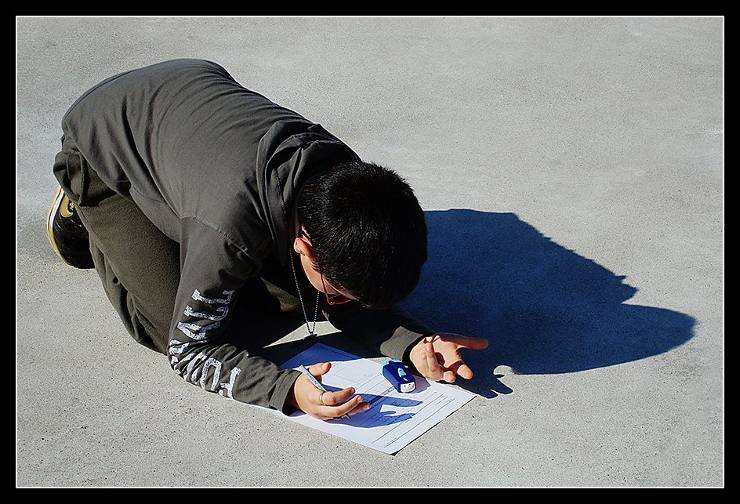
\includegraphics[width=0.95\textwidth]{/part08/llevo.jpg}
   \begin{center}
     {\large ``Y me llevo\ldots''}\par
     Foto di Sidi Guariach\par
     \url{http://www.flickr.com/photos/sidi_guariach/2240000519/}\par
    Licenza: Attribuzione 2.0 Generico (CC BY 2.0)\par
   \end{center}
\clearpage
\cleardoublepage
 
% (c) 2012 Tiziana Manca - tmanca@libero.it
% (c) 2012 - 2014 Dimitrios Vrettos - d.vrettos@gmail.com

\chapter{Relazioni}
%===================================
\section{Proposizioni e predicati}
In matematica frasi come ``19 è maggiore di~5'' o ``Giove ruota intorno alla Terra'' sono considerate \emph{proposizioni} perché ad esse
si può attribuire un preciso valore di verità, cioè si può stabilire se sono vere oppure false: la prima è una proposizione vera, la seconda è falsa.

Non sono proposizioni in senso matematico ``Cosa stai studiando?'', ``domani pioverà!'', ``$x$ è un numero primo'':
infatti la prima non è un'affermazione ma pone una domanda, la seconda è una esclamazione e quindi non possiamo stabilire se è vera o falsa;
l'ultima contiene un elemento indeterminato e finché non si fissa il valore da attribuire a~$x$, non si può decidere se la frase che lo riguarda è vera o falsa.

Ogni proposizione è formata da un \emph{predicato} (verbo) e dai suoi \emph{argomenti} (cose o persone alle quali il verbo si riferisce).

Analizzando le proposizioni sopra enunciate si ha:
\begin{center}
\begin{tabular}{llc}
\toprule
Soggetto & Predicato & Complemento \\
\midrule
19 & è maggiore di & 5 \\
Giove & ruota attorno alla & Terra \\
\bottomrule
\end{tabular}
\end{center}
Il soggetto e il complemento sono gli argomenti ai quali il predicato si riferisce.
In alcune proposizioni il predicato si riferisce a due argomenti (il \emph{soggetto} e il \emph{complemento})
in altre ad un solo argomento: ad esempio, il predicato ``essere numero primo'' stabilisce semplicemente una caratteristica del numero~5
senza porre alcuna connessione con un altro argomento.

\begin{definizione}\label{def:predicato_binario}
Si dice \emph{predicato binario} un predicato che si riferisce a due argomenti.
\end{definizione}

\ovalbox{\risolvi \ref{ese:B.1}}

\section{Relazioni in un insieme}

Il termine \emph{relazione} entra molto spesso in frasi del linguaggio naturale, lo usiamo per esprimere un generico legame tra due persone o tra due oggetti,
anche senza specificarne la natura: ``si è conclusa la relazione tra Anna e Paolo'', ``l'allungamento di una sbarretta di ferro è in relazione con il calore fornito'',
``la frana del terreno è in relazione con il disboscamento della zona e l'abusivismo edilizio'', ``domani consegnerò la relazione di fisica''.
Sono tutte espressioni che ci danno informazioni di un qualche collegamento tra gli
argomenti (persone, cose) ai quali il termine relazione si riferisce.

Dal punto di vista matematico diamo la seguente definizione.
\begin{definizione}
Si dice \emph{relazione} in un insieme~$A$ un predicato binario che lega due elementi dell'insieme.
\end{definizione}

\begin{exrig}
 \begin{esempio}
 Nell'insieme~$A = \{3\text{,~}5\text{,~}6\text{,~}9\text{,~}30\}$ è introdotto il predicato binario ``essere multiplo di''; con esso formiamo le proposizioni vere scegliendo soggetto e
 complemento nell'insieme~$A$:

\begin{multicols}{3}
30 è multiplo di~6;

9 è multiplo di~3;

30 è multiplo di~3;

6 è multiplo di~3;

30 è multiplo di~5;

3 è multiplo di~3;

5 è multiplo di~5;

6 è multiplo di~6;

9 è multiplo di~9;

30 è multiplo di~30.
\end{multicols}
Il predicato ``essere multiplo'' genera nell'insieme~$A$ una relazione matematica. Esso tuttavia non è il
solo che permette di collegare tra loro due elementi di quell'insieme.
\end{esempio}
\end{exrig}

\ovalbox{\risolvi \ref{ese:B.2}}

Se chiamiamo con~$\Rel$ il predicato binario che definisce la relazione introdotta nell'insieme, per indicare 
sinteticamente la proposizione avente come soggetto~$a$, come complemento~$b$ e come predicato~$\Rel$, scriviamo~$a \,\Rel\, b$ e
diremo che~\emph{$a$ è in relazione con~$b$}.

\begin{exrig}
 \begin{esempio}

Con riferimento all'esempio precedente si ha:~$A = \{3\text{,~}5\text{,~}6\text{,~}9\text{,~}30\}$ e $\Rel$:
``essere multiplo di''. Allora scriviamo: per qualunque~$a$ e~$b$ appartenenti ad~$A$,
$a \,\Rel\, b$ se e solo se~$a$ è multiplo di~$b$, in particolare:
\[30 \,\Rel\,~6;\quad~9 \,\Rel\,~3;\quad~30 \,\Rel\,~3;\quad~6 \,\Rel\,~3;\quad~30 \,\Rel\,~5;\quad~3 \,\Rel\,~3;\quad 5 \,\Rel\,~5;\quad~6 \,\Rel\,~6;\quad~9 \,\Rel\,~9;\quad~30 \,\Rel\,~30.\]
\end{esempio}
\end{exrig}

Abbiamo così formato un insieme di coppie ordinate di elementi tra loro in relazione:~$30 \,\Rel\,~5$ può anche essere indicata con la coppia ordinata~$(30;5)$.

\begin{definizione}
Chiamiamo \emph{insieme della relazione} $G_\Rel$ l'insieme delle coppie ordinate i cui
elementi sono gli argomenti del predicato binario, ossia sono in relazione tra di loro. Esso risulta essere un
sottoinsieme del prodotto cartesiano dell'insieme~$A$ con se stesso. Si rappresenta per proprietà caratteristica nel
seguente modo~$G_\Rel = \{(a;b) \in A \times A \mid  a \,\Rel\, b \}$.
\end{definizione}

\ovalbox{\risolvii \ref{ese:B.3}, \ref{ese:B.4}, \ref{ese:B.5}, \ref{ese:B.6}}
%===================================
\subsection{Grafico di una relazione}

Dal momento che una relazione in un insieme~$Y$ determina un sottoinsieme del prodotto cartesiano~$Y \times Y$, è
comodo rappresentare una relazione nello stesso diagramma usato per rappresentare il prodotto cartesiano.
Una relazione può quindi essere rappresentata attraverso un \emph{grafico cartesiano}.

\ovalbox{\risolvii \ref{ese:B.7}, \ref{ese:B.8}}

%===================================
\subsection{Matrice o tabella di una relazione}

Nella figura~\ref{fig:B.1} è rappresentata la classica griglia per il gioco della battaglia navale.
Ogni cella è individuata da una coppia ordinata il cui primo elemento (una lettera dell'alfabeto) indica la riga,
il secondo (un numero) indica la colonna; così la coppia~$(D;5)$ indica la cella annerita.

\ovalbox{\risolvii \ref{ese:B.9}, \ref{ese:B.10}, \ref{ese:B.11}}

%===================================
\subsection{Grafo di una relazione}

\begin{definizione}
Un \emph{grafo} è un insieme di punti, detti \emph{nodi}, e di archi che uniscono coppie di punti.
\end{definizione}

Abbiamo visto che con un predicato si possono formare alcune proposizioni aventi rispettivamente come soggetto e
come complemento elementi di un insieme: solo le proposizioni vere determinano la relazione tra gli elementi di
quell'insieme e generano coppie di elementi in relazione.

\begin{exrig}
 \begin{esempio}

Nel diagramma di Eulero-Venn di figura~\ref{fig:B.2}, relativo all'insieme~$A = \{$3, 5, 6, 9, 30$\}$
rappresentiamo la relazione~$\Rel$ = ``essere multiplo di'' collegando, mediante una freccia, gli argomenti delle proposizione vere.

Come puoi osservare, l'elemento~30 è collegato con una freccia all'elemento~6 in quanto la proposizione ``30 è multiplo di~6'' è vera, ma non all'elemento~9
poiché la proposizione ``30 è multiplo di~9'' è falsa; inoltre la punta della freccia è sul numero~6 in quanto complemento del predicato ``essere multiplo di'' (si parla in tal caso di \emph{grafo orientato});
infine su ciascun elemento abbiamo messo un ``anello'' o ``cappio'' per indicare che ogni elemento è in relazione con se stesso visto che per ogni
elemento~$a \in A$ la proposizione ``$a$ è multiplo di~$a$'' risulta vera.

 \end{esempio}
\end{exrig}

\ovalbox{\risolvii \ref{ese:B.12}, \ref{ese:B.13}, \ref{ese:B.14}, \ref{ese:B.15}, \ref{ese:B.16}, \ref{ese:B.17}, \ref{ese:B.18}}
\begin{figure}[hb]
\begin{minipage}[t]{.45\textwidth}
 \centering
 % (c) 2012 Dimitrios Vrettos - d.vrettos@gmail.com

\begin{tikzpicture}[x=10mm,y=10mm, font=\small,table nodes/.style={%
		rectangle,
		draw=black,
 		align=center,
   		minimum height=5mm,
     	text depth=0.5ex,
     	text height=1.5ex,
     	inner xsep=-1pt,
     	outer sep=0pt
	},
	table/.style={%
        matrix of nodes,
        row sep=-\pgflinewidth,
        column sep=-\pgflinewidth,
        nodes={%
            table nodes
        },
        execute at empty cell={\node[fill=black]{};}
    }]

\matrix (first) [table,text width=7mm,name=table]
{
{}  & 1 & 2 & 3 &4 & 5 & 6 & 7\\
$A$ &{} &{} &{} &{} &{} &{} &{} \\
$B$ &{} &{} &{} &{} &{} &{} &{} \\
$C$ &{} &{} &{} &{} &{} &{} &{} \\
$D$ &{} &{} &{} &{} & &{} &{}  \\
$E$ &{} &{} &{} &{} &{} &{} &{} \\
$F$ &{} &{} &{} &{} &{} &{} &{} \\
};

\end{tikzpicture}

 \caption{Griglia della battaglia navale.}\label{fig:B.1}
\end{minipage}\hfil
\begin{minipage}[t]{.45\textwidth}
 \centering
 % (c) 2012 Dimitrios Vrettos - d.vrettos@gmail.com

\begin{tikzpicture}[x=10mm,y=10mm, font=\small, every state/.style={draw=CornflowerBlue}, every loop/.style={draw=Maroon}]
\draw (0,0) circle (2);

\node[state] (5) at (-1.5,0) {5};
\node[state] (30) at (-.4,.8) {30};
\node[state] (6) at (1.1,.5) {6};
\node[state] (9) at (1,-1) {9};
\node[state] (3) at (-.5,-1.2) {3};

\begin{scope}[->]
\path(5) edge[loop below] node{} ()
	(30) edge[loop above] node{} ()
	(6) edge[loop above] node{} ()
	(9) edge[loop above] node{} ()
	(3) edge[loop left] node{} ();

\end{scope}
\begin{scope}[->, Maroon]
\draw (30)--(5);
\draw (30)--(6);
\draw (30)--(3);
\draw (6)--(3);
\draw (9)--(3);
\end{scope}
\end{tikzpicture}

 \caption{L'insieme~$A$.}\label{fig:B.2}
\end{minipage}
\end{figure}

\pagebreak
\section{Proprietà delle relazioni}
%===================================
\subsection{Proprietà riflessiva}

\begin{exrig}
 \begin{esempio}

Nell'insieme~$T = \{\text{7, 8, 12, 34, 100}\}$ è introdotta la relazione~$\Rel$: ``essere divisore di''.
Puoi verificare che ogni numero è divisore di se stesso, cioè ogni elemento dell'insieme è in relazione
con se stesso. Una relazione di questo tipo si dice che gode della \emph{proprietà riflessiva}.
Osserva, però, che nell'insieme ~$\insN$ dei numeri naturali la relazione ``essere divisibile per'' non è riflessiva poiché zero non è divisibile per se stesso.
 \end{esempio}
\end{exrig}

\begin{definizione}
Una relazione~$\Rel$ in un insieme~$A$ gode della \emph{proprietà riflessiva} quando ogni elemento è in relazione con se stesso, ossia per qualunque~$x$ dell'insieme~$A$ si ha~$x \,\Rel\, x$.
\end{definizione}

\ovalbox{\risolvi \ref{ese:B.19}}

%===================================
\subsection{Proprietà antiriflessiva}

\begin{exrig}
 \begin{esempio}
Nell'insieme delle persone~$P = \{\text{Marco, Antonio, Carlo}\}$ è data la relazione~$\Rel$: ``essere più alto di''
rappresentata con la figura~\ref{fig:B.3} di pagina~\pageref{fig:B.3}.
Puoi notare che nessun elemento è in relazione con se stesso. In effetti nessuno può essere più alto di se stesso.

 \end{esempio}
\end{exrig}

\begin{definizione}
Una relazione~$\Rel$ in un insieme~$A$ gode della \emph{proprietà antiriflessiva} quando nessun elemento è in relazione con se stesso,
ossia per nessun elemento~$x$ di~$A$ si ha~$x \,\Rel\, x$.
\end{definizione}

\ovalbox{\risolvi \ref{ese:B.20}}
\subsection{Proprietà simmetrica}

\begin{exrig}
 \begin{esempio}
Nella figura~\ref{fig:B.4} a pagina~\pageref{fig:B.4} è rappresentata la relazione~$\Rel$: ``essere concorde con'' nell'insieme dei numeri~$A = \{-1\text{, }+3\text{, }-7\text{, }+5\text{, }-2\text{, }+4\text{, }+10\}$.
Per collegare elementi in relazione abbiamo usato archi anziché frecce poiché, ad esempio, le proposizioni ``$+3$ è concorde con~$+10$'' e ``$+10$ è concorde con~$+3$''
sono entrambe vere. Per questa relazione si può osservare che se un elemento dell'insieme è in relazione con un altro allora anche quest'ultimo è in relazione con il primo:
$-1 \,\Rel\, -7$, ma anche~$-7 \,\Rel\, -1$; $+3 \,\Rel\, +5$, ma anche~$+5 \,\Rel\, +3$ e così via.
 \end{esempio}
\end{exrig}

\begin{figure}[ht]
\begin{minipage}[t]{.45\textwidth}
 \centering
 % (c) 2012 Dimitrios Vrettos - d.vrettos@gmail.com

\begin{tikzpicture}[x=10mm,y=10mm, font=\small, every state/.style={draw=CornflowerBlue}, every loop/.style={draw=Maroon}]
\draw (0,0) circle (1.8);

\node at (1.8,1.5) {$P$};

\node[state] (M) at (-1,.3) {$M$};
\node[state] (C) at (.8,.8) {$C$};
\node[state] (A) at (.2,-1) {$A$};

 \begin{scope}[->, Maroon]
 \draw (M)--(C);
 \draw (M)--(A);
 \draw (C)--(A);
 \end{scope}
\end{tikzpicture}
 \caption{Proprietà antiriflessiva.}\label{fig:B.3}
\end{minipage}\hfil
\begin{minipage}[t]{.45\textwidth}
 \centering
 % (c) 2012 Dimitrios Vrettos - d.vrettos@gmail.com

\begin{tikzpicture}[x=10mm,y=10mm, font=\small, every state/.style={draw=CornflowerBlue}, every loop/.style={draw=Maroon}]
\draw (0,0) circle [x radius=3, y radius=2];

\node[state] (A) at (-2.3,.3) {$-1$};
\node[state] (B) at (-.8,1.2) {$-2$};
\node[state] (C) at (-1.5,-1) {$-7$};
\node[state] (D) at (-.5,-.9) {$+10$};
\node[state] (E) at (.6,.9) {$+3$};
\node[state] (F) at (1.8,.5) {$+4$};
\node[state] (G) at (1.5,-1) {$+5$};

\begin{scope}[->]
\path(A) edge[loop below] node{} ()
	(B) edge[loop right] node{} ()
	(C) edge[loop left] node{} ()	
(D) edge[loop below] node{} ()
	(E) edge[loop above] node{} ()
	(F) edge[loop right] node{} ()
	(G) edge[loop right] node{} ();

\end{scope}
% \begin{scope}[<->, Maroon]
 \begin{scope}[-, Maroon]
 \draw (A)--(C);
 \draw (B)--(A);
 \draw (C)--(B);
\draw (D)--(E);
\draw (D)--(F);
\draw (E)--(F);
\draw (G)--(F);
\draw (E)--(G);
\draw (D)--(G);
 \end{scope}
\end{tikzpicture}

 \caption{Proprietà simmetrica.}\label{fig:B.4}
\end{minipage}
\end{figure}

\begin{definizione}
Una relazione~$\Rel$ in un insieme~$A$ gode della \emph{proprietà simmetrica} quando risultano vere le due proposizioni
che si ottengono scambiando soggetto e complemento; ossia per qualunque~$x$ e~$y$ appartenenti all'insieme~$A$ se vale~$x \,\Rel\, y$
allora vale anche~$y \,\Rel\, x$.
\end{definizione}

\ovalbox{\risolvi \ref{ese:B.21}}

%===================================
\subsection{Proprietà antisimmetrica}

\begin{exrig}
 \begin{esempio}

Il diagramma di Venn nella figura~\ref{fig:B.5} rappresenta un insieme~$U$ e alcuni suoi sottoinsiemi.

Consideriamo ora l'insieme di insiemi~$S = \{U\text{,~}A\text{,~}B\text{,~}C\text{,~}D\text{,~}E\text{,~}F\}$ e la relazione~$\Rel$: ``essere sottoinsieme proprio di''.
Completa il grafo della relazione.

Certamente nel completare il grafo (figura~\ref{fig:B.6}) non avrai usato archi poiché è evidente che le proposizioni ``$B$ è sottoinsieme proprio di~$C$'' e ``$C$
è sottoinsieme proprio di~$B$'' non possono essere entrambe vere. Anzi, la verità della prima implica necessariamente la falsità della seconda.
 \end{esempio}
\end{exrig}

\begin{figure}[hb]
\begin{minipage}[b]{.45\textwidth}
 \centering
 % (c) 2012 Dimitrios Vrettos - d.vrettos@gmail.com

\begin{tikzpicture}[scale=.7,x=10mm,y=10mm, font=\small, every state/.style={draw=CornflowerBlue}, every loop/.style={draw=Maroon}]
\draw (0,0) circle [x radius=2, y radius=1.5] node {$A$};
\draw[CornflowerBlue] (-.5,-.7) circle [x radius=.8, y radius=.5]node {$E$};
\draw[OliveGreen] (1,.5) circle [x radius=.4, y radius=.2]node {$B$};
\draw[Maroon] (3,.5) circle [x radius=3, y radius=.5]node {$C$};
\draw[OliveGreen] (3.5,-.8) circle [x radius=1.5, y radius=.5]node {$D$};
\draw[RedOrange] (4.2,-.8) circle [x radius=.5, y radius=.25]node {$F$};

\node () at (2.1,2) {$U$};
\end{tikzpicture}
 \caption{L'insieme~$U$.}\label{fig:B.5}
\end{minipage}\hfil
\begin{minipage}[b]{.45\textwidth}
 \centering
 % (c) 2012 Dimitrios Vrettos - d.vrettos@gmail.com

\begin{tikzpicture}[scale=.7,x=10mm,y=10mm, font=\small, every state/.style={draw=CornflowerBlue}, every loop/.style={draw=Maroon}]
\draw (0,0) circle [x radius=3, y radius=2];

\node at (3,1.5) {$S$};
\node[state] (A) at (-2.3,.3) {$A$};
\node[state] (B) at (-.8,1.2) {$B$};
\node[state] (C) at (-1.5,-1) {$C$};
\node[state] (D) at (-.2,-1.1) {$D$};
\node[state] (E) at (.6,.9) {$E$};
\node[state] (F) at (1.8,.5) {$F$};
\node[state] (U) at (1.5,-1) {$U$};

  \begin{scope}[->, Maroon]
 \draw (A)--(U);
  \draw (B)--(C);
 \draw (F)--(U);
   \end{scope}
\end{tikzpicture}
 \caption{L'insieme~$S$.}\label{fig:B.6}
\end{minipage}
\end{figure}

\begin{definizione}
Una relazione~$\Rel$ in un insieme~$A$ gode della \emph{proprietà antisimmetrica} quando non possono essere vere
contemporaneamente le proposizioni che si ottengono scambiando il soggetto con il complemento, se soggetto e complemento sono diversi
tra loro; ossia per qualunque~$x$ e~$y$ dell'insieme~$A$ se~$x \neq y$ e se~$x \,\Rel\, y$ non è vero che~$y \,\Rel\, x$.
\end{definizione}

\ovalbox{\risolvi \ref{ese:B.22}}

%===================================
\subsection{Proprietà transitiva}

\begin{exrig}
 \begin{esempio}

Nel grafo di figura~\ref{fig:B.7} è rappresentata una relazione~$\Rel$ introdotta in un insieme~$T$. Dall'analisi della situazione rappresentata possiamo
affermare che dalla verità di $a \,\Rel\, b$ e~$b \,\Rel\, c$ segue la verità di~$a \,\Rel\, c$. Analizzando gli altri elementi, 
possiamo osservare che essendo vere $e \,\Rel\, f$ e~$f\, \Rel\, g$ è vera anche~$e \,\Rel\, g$;
inoltre si ha che essendo vera $n \,\Rel\, m$ e~$m \,\Rel\, t$ è vera anche~$n \,\Rel\, t$.
 \end{esempio}
\end{exrig}

\begin{figure}[ht]
\begin{minipage}[b]{.45\textwidth}
 \centering
 % (c) 2012 Dimitrios Vrettos - d.vrettos@gmail.com

\begin{tikzpicture}[x=10mm,y=10mm, font=\small, every state/.style={draw=CornflowerBlue}, every loop/.style={draw=Maroon}]
\draw (0,0) circle [x radius=3, y radius=2];

\node at (3,1.5) {$T$};
\node[state] (A) at (-2.3,.3) {$a$};
\node[state] (B) at (-.8,1.2) {$b$};
\node[state] (C) at (-1,0) {$c$};
\node[state] (G) at (.2,0) {$g$};
\node[state] (E) at (.6,1.3) {$e$};
\node[state] (F) at (1.8,.8) {$f$};
\node[state] (M) at (1.5,-1.1) {$m$};
\node[state] (N) at (0,-1.2) {$n$};
\node[state] (T) at (2.2,-.2) {$t$};
\begin{scope}[->, Maroon]
\draw (A)--(C);
\draw (B)--(C);
\draw (A)--(B);

\draw (E)--(F);
\draw (E)--(G);
\draw (F)--(G);

\draw (N)--(M);
\draw (N)--(T);
\draw (M)--(T);
\end{scope}
\end{tikzpicture}
 \caption{L'insieme~$T$.}\label{fig:B.7}
\end{minipage}\hfil
\begin{minipage}[b]{.45\textwidth}
 \centering
 % (c) 2012 Dimitrios Vrettos - d.vrettos@gmail.com

\begin{tikzpicture}[x=10mm,y=10mm, font=\small, every state/.style={draw=CornflowerBlue}, every loop/.style={draw=Maroon}]
\draw (0,0) circle [x radius=3, y radius=2];

\node at (3,1.5) {$B$};
\node[state] (A) at (-2.3,.3) {$a$};
\node[state] (H) at (-.8,1.2) {$h$};
\node[state] (F) at (-1.5,-1) {$f$};
\node[state] (B) at (-.5,-.3) {$b$};
\node[state] (E) at (.6,.9) {$e$};
\node[state] (C) at (1.8,.5) {$c$};
\node[state] (D) at (1.5,-.5) {$d$};
\node[state] (G) at (.5,-1.3) {$g$};
\begin{scope}[->]
\path(A) edge[loop below] node{} ()
(H) edge[loop right] node{} ()
(F) edge[loop left] node{} ()	
(B) edge[loop below] node{} ()
(E) edge[loop above] node{} ()
(C) edge[loop right] node{} ()
(D) edge[loop right] node{} ()
(G) edge[loop above] node{} ();
\end{scope}
\begin{scope}[-, Maroon]
\draw (A)--(H);
\draw (F)--(A);
\draw (F)--(H);
\draw (B)--(E);
\draw (B)--(C);
\draw (E)--(C);
\draw (G)--(D);
\end{scope}
\end{tikzpicture}
 \caption{L'insieme~$B$.}\label{fig:B.8}
\end{minipage}
\end{figure}

\begin{definizione}
Una relazione~$\Rel$ in un insieme~$A$ gode della \emph{proprietà transitiva} quando se~$a \,\Rel\, b$ e~$b \,\Rel\, c$
allora risulta anche~$a \,\Rel\, c$, con~$a$, $b$, $c$ elementi qualsiasi dell'insieme~$A$.
\end{definizione}

\ovalbox{\risolvii \ref{ese:B.23}, \ref{ese:B.24}, \ref{ese:B.25}, \ref{ese:B.26}, \ref{ese:B.27}, \ref{ese:B.28}, \ref{ese:B.29}}

%===================================
\section{Relazioni di equivalenza}

\begin{exrig}
 \begin{esempio}

Completa la seguente tabella segnando le proprietà di cui gode (R=riflessiva, S=simmetrica, T=transitiva) ciascuna relazione indicata.

\begin{center}
\begin{tabular}{lcc}
\toprule
Relazione & Insieme & Proprietà \\
\midrule
Avere lo stesso perimetro & poligoni & \boxR\quad\boxS\quad\boxT \\
Essere fratello di & persone & \boxR\quad\boxS\quad\boxT \\
Essere figlio di & persone & \boxR\quad\boxS\quad\boxT \\
Essere più alto di & persone & \boxR\quad\boxS\quad\boxT \\
Avere gli angoli rispettivamente congruenti & triangoli & \boxR\quad\boxS\quad\boxT \\
Iniziare con la stessa lettera & parole & \boxR\quad\boxS\quad\boxT \\
Giocare nella stessa squadra & calciatori & \boxR\quad\boxS\quad\boxT \\
$(a;b) \,\Rel\, (x;y)$ se e solo se~$a+b=x+y$ & ~$\insN \times \insN$ & \boxR\quad\boxS\quad\boxT \\
\bottomrule
\end{tabular}
\end{center}

\emph{Svolgimento}: La prima relazione gode delle tre proprietà riflessiva, simmetrica e transitiva; infatti:

\begin{itemize*}
\item ``il poligono~$P$ ha lo stesso perimetro di se stesso'' è vera per qualunque poligono (\emph{proprietà riflessiva});
\item ``il poligono~$P_1$ ha lo stesso perimetro del poligono~$P_2$'' implica la verità della proposizione ``il
poligono~$P_2$ ha lo stesso perimetro di~$P_1$'', qualunque siano i due poligoni~$P_1$ e~$P_2$ (\emph{proprietà
simmetrica});
\item se ``il poligono~$P_1$ ha lo stesso perimetro di~$P_2$'' e ``$P_2$ ha lo stesso perimetro di~$P_3$'' allora si ha anche che ``$P_1$ ha lo stesso
perimetro di~$P_3$'', qualunque siano i poligoni~$P_1$, $P_2$, $P_3$ (\emph{proprietà transitiva}).
\end{itemize*}

Verifica tu se anche le altre relazioni godono delle tre proprietà riflessiva, simmetrica, transitiva, come
``essere fratello di'', ``avere gli angoli rispettivamente uguali'', ``iniziare con la stessa lettera''.
 \end{esempio}
\end{exrig}

\begin{definizione}
Chiamiamo \emph{relazione d'equivalenza} una relazione che gode delle tre proprietà riflessiva, simmetrica e transitiva.
\end{definizione}

\ovalbox{\risolvii \ref{ese:B.30}, \ref{ese:B.31}}

\begin{exrig}
 \begin{esempio}

Dato l'insieme~$B = \{a\text{, }b\text{, }c\text{, }d\text{, }e\text{, }f\text{, }g\text{, }h\}$ e la relazione rappresentata dal grafo di figura~\ref{fig:B.8} a pagina~\pageref{fig:B.8}, costruiamo alcuni suoi sottoinsiemi seguendo le istruzioni:
\begin{itemize*}
\item \emph{ripeti \ldots{}};
\item scegliamo a caso un elemento di~$B$;
\item formiamo un sottoinsieme contenente l'elemento scelto e tutti gli altri che con quello sono in relazione;
\item \emph{\ldots{} finché} non abbiamo esaurito tutti gli elementi.
\end{itemize*}


\emph{Svolgimento}:
\begin{itemize*}
\item scegliamo l'elemento~$a$ e definiamo il sottoinsieme~$B_1$ avente come elementi~$a$, $h$, $f$ che sono in relazione con~$a$:~$B_1 = \{a\text{, }h\text{, }f\}$.
Gli elementi di~$B$ non sono esauriti, quindi ripetiamo i passi scegliendo un elemento tra quelli rimasti;
\item scegliamo~$g$ e formiamo il sottoinsieme~$B_2$ avente come elementi~$g$ e~$d$, l'unico che con esso è in relazione:~$B_2 = \{g\text{, }d\}$.
Gli elementi dell'insieme~$B$ non sono esauriti, quindi ripetiamo i passi scegliendo un elemento tra quelli rimasti;
\item scegliamo~$c$ e formiamo il sottoinsieme~$B_3$ avente come elementi~$c$, $e$, $b$ che con esso sono in relazione:~$B_3 = \{c\text{, }e\text{, }b\}$.
\end{itemize*}

Gli elementi dell'insieme assegnato sono stati esauriti. Abbiamo così ottenuto tre sottoinsiemi dell'insieme~$B$ (figura~\ref{fig:B.9} a pagina~\pageref{fig:B.9}) che hanno queste particolari caratteristiche:

\begin{itemize*}
\item nessuno di essi è vuoto;
\item a due a due sono disgiunti (non hanno tra loro alcun elemento in comune);
\item la loro unione è l'insieme~$B$.
\end{itemize*}
 \end{esempio}
\end{exrig}

\begin{figure}[ht]
\begin{minipage}[t]{.45\textwidth}
 \centering
 % (c) 2012 Dimitrios Vrettos - d.vrettos@gmail.com

\begin{tikzpicture}[scale=.8,x=10mm,y=10mm, font=\small, every state/.style={draw=CornflowerBlue}, every loop/.style={draw=Maroon}]
\draw (0,0) circle [x radius=3, y radius=2];

\node at (3,1.5) {$B$};
\begin{scope}[dotted]
\draw (0,2) -- (-1.5,-1.73);
\draw (0,2) -- (1.5,-1.73);
\end{scope}
\node[state] (A) at (-2.3,.3) {$a$};
\node[state] (H) at (-1,1.2) {$h$};
\node[state] (F) at (-1.8,-1) {$f$};
\node[state] (B) at (1,1) {$b$};
\node[state] (E) at (1.9,.2) {$e$};
\node[state] (C) at (1.8,-1) {$c$};
\node[state] (D) at (0,.1) {$d$};
\node[state] (G) at (0,-1.3) {$g$};

\node at (-2.5,-2) {$B_1$};
\node at (0,-2.5) {$B_2$};
\node at (2.5,-2) {$B_3$};

\end{tikzpicture}
 \caption{I sottoinsiemi dell'insieme~$B$.}\label{fig:B.9}
\end{minipage}\hfil
\begin{minipage}[t]{.45\textwidth}
 \centering
 % (c) 2012 Dimitrios Vrettos - d.vrettos@gmail.com

\begin{tikzpicture}[scale=.8,x=10mm,y=10mm, font=\small, every state/.style={draw=CornflowerBlue}, every loop/.style={draw=Maroon}]
\draw (0,0) circle [x radius=3, y radius=2];

\node at (3,1.5) {$P(B)$};
\begin{scope}[dotted]
\draw (0,2) -- (-1.5,-1.73);
\draw (0,2) -- (1.5,-1.73);
\end{scope}
\node[state] (A) at (-2.3,.3) {$a$};
\node[state] (H) at (-1,1.2) {$h$};
\node[state] (F) at (-1.8,-1) {$f$};
\node[state] (B) at (1,1) {$b$};
\node[state] (E) at (1.9,.2) {$e$};
\node[state] (C) at (1.8,-1) {$c$};
\node[state] (D) at (0,.1) {$d$};
\node[state] (G) at (0,-1.3) {$g$};

\node at (-2.5,-2) {$[a]$};
\node at (0,-2.5) {$[d]$};
\node at (2.5,-2) {$[b]$};

\end{tikzpicture}
 \caption{La partizione dell'insieme~$B$ in classi d'equivalenza.}\label{fig:B.10}
\end{minipage}
\end{figure}
\pagebreak
Premettiamo le definizioni:

\begin{definizione}
Dato un insieme $A$, suddividiamolo in un numero di sottoinsiemi~$A_1$, $A_2$, \ldots, $A_n$, detti \emph{classi}, tali che
\begin{enumeratea}
\item nessun sottoinsieme è vuoto;
\item a due a due sono disgiunti (non hanno tra loro alcun elemento in comune);
\item la loro unione è l'insieme~$A$.
\end{enumeratea}
L'insieme $P(A) = \{A_1$, $A_2$, \ldots, $A_n\}$ è detto \emph{partizione} di~$A$.
\end{definizione}

\begin{definizione}
In un insieme~$A$ dove sia stata definita una relazione d'equivalenza $\Rel$, si chiama \emph{classe d'equivalenza} ogni sottoinsieme di~$A$ contenente tutti e soli gli elementi
tra loro in relazione secondo $\Rel$.
\end{definizione}

Si viene così a determinare una partizione dell'insieme~$A$ in classi d'equivalenza, ognuna delle quali è indicata racchiudendo tra parentesi quadrate
uno degli elementi della classe considerata.
Nell'esempio sopra riportato le classi d'equivalenza sono i sottoinsiemi di~$B$ indicati con~$[a]$, $[b]$, $[d]$; la
partizione dell'insieme~$B$ in classi d'equivalenza è rappresentata con il diagramma di Eulero-Venn nella figura~\ref{fig:B.10}.

\begin{definizione}
Si chiama \emph{insieme quoziente} di un insieme~$A$ rispetto alla relazione di equivalenza~$\Rel$ in esso definita,
l'insieme i cui elementi sono le classi d'equivalenza determinate dalla relazione~$\Rel$, ovvero la partizione di~$A$ definita da~$\Rel$. L'insieme quoziente si indica con il simbolo~$A/\Rel$.
\end{definizione}

Nel caso dell'esempio precedente l'insieme quoziente~$B/\Rel$ è quello riportato nel seguente diagramma di Eulero-Venn:
\begin{center}
 % (c) 2012 Dimitrios Vrettos - d.vrettos@gmail.com

\begin{tikzpicture}[scale=.9,x=10mm,y=10mm, font=\small]
\draw (0,0) circle [x radius=1.3, y radius=1.3];

\node at (1.3,1.3) {$B/\Rel$};

\begin{scope}[fill=CornflowerBlue]
\fill  (0,0)circle (1.5pt) node[above right] {$[a]$};
\fill (-.5,.7) circle (1.5pt)node[above right] {$[b]$};
\fill(-.5,-.7) circle (1.5pt)node[above right] {$[d]$};
\end{scope}
\end{tikzpicture}

\end{center}

\osservazione Ogni volta che si ha una relazione d'equivalenza~$\Rel$ in un insieme~$A$, possiamo stabilire la seguente
catena di passaggi:
 \[\text{insieme }A\rightarrow\Rel\rightarrow\text{ partizione }P(A)=\text{ insieme quoziente }A/\Rel.\]

\ovalbox{\risolvii \ref{ese:B.32}, \ref{ese:B.33}, \ref{ese:B.34}, \ref{ese:B.35}, \ref{ese:B.36}, \ref{ese:B.37}, \ref{ese:B.38}, \ref{ese:B.39}, \ref{ese:B.40},
\ref{ese:B.41}, \ref{ese:B.42}}

\ovalbox{\ref{ese:B.43}}

\section{Relazioni di ordine}

Nel linguaggio di ogni giorno avrai certamente spesso usato espressioni come ``devo mettere in ordine i miei
libri'' oppure ``qui non c'è ordine'' e altre espressioni simili.
Anche in matematica, fin dalla scuola elementare, hai imparato a ordinare gli elementi dell'insieme dei
numeri naturali: dati due numeri naturali hai imparato infatti a stabilire quale dei due è il maggiore.

\begin{definizione}
Una relazione~$\Rel$, introdotta in un insieme~$A$, si chiama \emph{relazione d'ordine} se è antisimmetrica e transitiva.
\end{definizione}

Riguardando le varie relazioni introdotte sin qui, possiamo stabilire che esistono relazioni d'ordine di vario tipo, schematizzate nel seguente diagramma:
\begin{center}
 % (c) 2012 Dimitrios Vrettos - d.vrettos@gmail.com

\begin{tikzpicture}[x=10mm,y=10mm, font=\small]

\node {Relazione d'ordine}[grow=right,level distance= 30mm, sibling distance=15mm,->,thick, draw=Maroon]
child {node {parziale}[sibling distance=10mm]
child {node {in senso largo}}
child {node {in senso stretto}}}
child {node {totale}[sibling distance=10mm]
child {node {in senso largo}}
child {node {in senso stretto}}};

\end{tikzpicture}

\end{center}

Attraverso alcuni esempi, vogliamo chiarire le differenze tra i diversi tipi. A questo scopo introduciamo la seguente definizione.

\begin{definizione}
Data una relazione d'ordine~$\Rel$ definita in un insieme~$A$, due elementi distinti~$x$ e~$y$ sono \emph{confrontabili} se rispetto a~$\Rel$ si ha~$x \,\Rel\, y$ oppure~$y \,\Rel\, x$.
\end{definizione}

\begin{exrig}
 \begin{esempio}

In base al diagramma di Eulero-Venn riportato nella figura~\ref{fig:B.5} a pagina~\pageref{fig:B.5}, introduciamo nell'insieme~$S = \{U$, $A$, $B$, $C$, $D$, $E$, $F\}$ la relazione~$\Rel$: ``essere sottoinsieme di''.
Ricordiamo che, dati due insiemi~$X$ e~$Y$, $X$ è \emph{sottoinsieme} di~$Y$, in simboli $X \subseteq Y$, quando ogni elemento di~$X$ appartiene a~$Y$.

Vogliamo studiare le proprietà della relazione~$\Rel$:

\begin{enumeratea}
\item poiché ogni insieme è sottoinsieme di se stesso, possiamo dire che~$\Rel$ è riflessiva;
\item se~$X \subseteq Y$ e~$X \neq Y$ allora~$Y \not\subseteq X$ quindi~$\Rel$ è una relazione antisimmetrica;
\item se~$X \subseteq Y$ e~$Y \subseteq Z$ allora~$X \subseteq Z$ quindi~$\Rel$ è una relazione transitiva.
\end{enumeratea}

Inoltre è evidente che esistono almeno due elementi dell'insieme~$S$ che non sono in
alcun modo in relazione: ad esempio~$A \not\subseteq D$ e~$D \not\subseteq A$, ossia~$A$ e~$D$ non sono confrontabili.

 \end{esempio}

 \begin{esempio}

Riprendiamo il diagramma di Eulero-Venn dell'esempio precedente e introduciamo nell'insieme~$S = \{U$, $A$, $B$, $C$, $D$, $E$, $F\}$ la relazione~$\Rel$:
``essere sottoinsieme proprio di''. Studiamo le proprietà di questa relazione:
\begin{itemize*}
 \item cosa è cambiato rispetto alla relazione precedente? $\ldots$
 \item sono ancora valide le proprietà antisimmetrica e transitiva? $\ldots$
 \item esistono elementi di~$S$ non confrontabili? $\ldots$
\end{itemize*}

 \end{esempio}
\end{exrig}

\begin{definizione}
Una relazione d'ordine si dice \emph{parziale} quando esistono almeno due elementi che non sono confrontabili.
\end{definizione}

\begin{definizione}
Una relazione d'ordine si dice \emph{totale} quando due qualsiasi elementi possono essere messi in relazione, cioè sono confrontabili.
\end{definizione}

\begin{definizione}
Una relazione d'ordine è detta \emph{in senso largo} quando essa gode della proprietà riflessiva.
\end{definizione}

\begin{definizione}
Una relazione d'ordine è detta \emph{in senso stretto} quando essa gode della proprietà antiriflessiva.
\end{definizione}

\begin{center}
 % (c) 2012 Dimitrios Vrettos - d.vrettos@gmail.com

\begin{tikzpicture}[x=10mm,y=10mm, font=\small]

\node {Relazione d'ordine}[grow=right,level distance= 40mm,->,thick, draw=Maroon]
child {node {parziale (elementi non tutti confrontabili)}[level distance=55mm,sibling distance=10mm]
child {node {in senso largo (riflessiva)}}
child {node {in senso stretto (antiriflessiva)}}}
child {node {totale (elementi tutti confrontabili)}[level distance=55mm,sibling distance=10mm]
child {node {in senso largo (riflessiva)}}
child {node {in senso stretto (antiriflessiva)}}};

\end{tikzpicture}

\end{center}

\ovalbox{\risolvii \ref{ese:B.44}, \ref{ese:B.45}, \ref{ese:B.46}, \ref{ese:B.47}, \ref{ese:B.48}, \ref{ese:B.49}, \ref{ese:B.50}, \ref{ese:B.51},
\ref{ese:B.52}, \ref{ese:B.53}, \ref{ese:B.54}}

\ovalbox{ \ref{ese:B.55}, \ref{ese:B.56}, \ref{ese:B.57}, \ref{ese:B.58}, \ref{ese:B.59}, \ref{ese:B.60},
\ref{ese:B.61},\ref{ese:B.62}, \ref{ese:B.63}}
\newpage
% (c) 2012 Silvia Cibola - silvia.cibola@gmail.com
% (c) 2012 - 2014 Dimitrios Vrettos - d.vrettos@gmail.com

\section{Esercizi}

\subsection{Esercizi dei singoli capitoli}

\subsubsection*{B.1 - Prime definizioni}
\begin{esercizio}
\label{ese:B.1}
Segnate nel piano dotato di riferimento cartesiano ortogonale i vettori~$\vec{v}(1;2)$ e~$\vec{w}(3;-1)$. Possiamo affermare che~$|\vec{w}|=2 \cdot |\vec{v}|$?
\end{esercizio}

\subsubsection*{B.2 - Operazioni con i vettori}
\begin{esercizio}
\label{ese:B.2}
Provate a giustificare la seguente affermazione: l'operazione di addizione definita secondo la regola del parallelogramma gode della proprietà commutativa.
\end{esercizio}

\begin{esercizio}
\label{ese:B.3}
Determinate il vettore~$\vec{z}=\vec{u}+\vec{w}$ essendo~$\vec{u}(-1;-3)$ e~$\vec{v}(2;-1)$. Determinate inoltre il modulo di~$\vec{z}$ e la sua direzione.
Potete affermare che~$|\vec{z}|=|\vec{u}|+|\vec{w}|$?
\end{esercizio}

\begin{esercizio}
\label{ese:B.4}
Nel riferimento cartesiano ortogonale riportato di seguito sono rappresentati i vettori~$\vec{u}$ e~$\vec{v}$. Completate:

\begin{enumeratea}
\item il vettore~$\vec{u}$ è applicato all'origine e ha componenti~$\ldots$;
\item il vettore~$\vec{v}$ ha il primo estremo in~$B(\ldots;\ldots)$ e il secondo in~$\ldots$, pertanto le sue componenti sono~$\ldots$;
\item $m_{\vec{u}}=\ldots$ e~$m_{\vec{v}}=\ldots$, pertanto essi sono~$\ldots$;
\item $|\vec{u}|=\ldots$ e~$|\vec{v}|=\ldots$;
\item determinare~$r$ in modo che~$\vec{v}=r \cdot \vec{u}$.
\end{enumeratea}
\begin{center}
 % (c) 2012 Dimitrios Vrettos - d.vrettos@gmail.com

\begin{tikzpicture}[x=7mm,y=7mm, font=\small]

  \begin{scope}[->]
    \draw (-3.5,0) -- (3.5,0) node [below right] {$x$};
    \draw (0,-.5) -- (0,8.5) node[above left] {$y$};
  \end{scope}

  \foreach \x/\xtext in {-3/-3,-2/-2,-1/-1,1/1,2/2,3/3}{
    \node[below] at (\x,0) {$\xtext$};
    \draw (\x,1.5pt) -- (\x,-1.5pt);}
  \foreach \y/\ytext in {1/1,2/2,3/3,4/4,5/5,6/6,7/7,8/8}{
    \node[left] at (0,\y) {$\ytext$};
    \draw (1.5pt,\y) -- (-1.5pt,\y);}
  \node[below left] at (0,0) {$0$};

  \begin{scope}[dotted, orange, step=7mm]
    \draw (-3.5,-.5) grid (3.5,8.5);
  \end{scope}

  \begin{scope}[thick, ->,shorten >=1.5pt]
	\draw[Maroon] (0,0) -- (3,3);  
	\draw[OliveGreen](-3,3) -- (3,8);
      \end{scope}
 

\begin{scope}[fill=CornflowerBlue, draw=black]
\filldraw (0,0) circle (1.5pt)node [above left]{$O$};
\filldraw (3,3) circle (1.5pt)node [above right]{$A$};
\filldraw (-3,3) circle (1.5pt)node [below left]{$B$};
\filldraw (3,8) circle (1.5pt) node [above right]{$C$};
\end{scope}
\node[above] at (1.5,1.5) {$\vec{u}$};
\node[above] at (.5,6) {$\vec{v}$};
\end{tikzpicture}
\end{center}

\end{esercizio}

\begin{esercizio}
\label{ese:B.5}
Determinate le componenti del vettore~$\vec{w}=2 \cdot \vec{v}$ essendo~$\vec{v}(\frac{3}{2};-2)$. Verificate che~$\vec{w}$ e~$\vec{v}$ hanno stessa direzione
e~$|\vec{w}|=2 \cdot |\vec{v}|$.
\end{esercizio}

\begin{esercizio}
\label{ese:B.6}
Verificate che~$\frac{3}{2} \cdot (\vec{x}+\vec{y})=\frac{3}{2}\vec{x}+\frac{3}{2}\vec{y}$ essendo~$\vec{x}(-\frac{5}{4};1)$ e~$\vec{y}(4;-1)$.
\end{esercizio}
\pagebreak
\subsubsection*{B.3 - Dipendenza e indipendenza lineare}
\begin{esercizio}
\label{ese:B.7}
Completate le scritture:
\begin{multicols}{2}
\begin{enumeratea}
\item $\vec{v}(-\sqrt{2};\frac {5}{4})=\ldots \cdot \vec{i}+\ldots \cdot \vec{j}$;
\item $\vec{u}(1;-1)=\ldots \cdot \vec{i}+\ldots \cdot \vec{j}$;
\item $\vec{h}(\ldots;\ldots)=\frac {\sqrt{3}}{3} \cdot \vec{i}-9 \cdot \vec{j}$;
\item $\vec{z}(\ldots;\ldots)=\frac {3 \sqrt{5}}{3} \cdot \vec{i}$;
\end{enumeratea}
\end{multicols}
\end{esercizio}

\begin{esercizio}
\label{ese:B.8}
\begin{multicols}{2}
 Dati i vettori della figura a fianco, applicate il metodo geometrico per determinare i vettori che permettono di scrivere~$\vec{w}$ come combinazione lineare degli altri due.
Riprendete questi stessi vettori e determinate i vettori che permettono di scrivere~$\vec{v}$ come combinazione lineare degli altri due. In maniera analoga, determinate i vettori che permettono di scrivere~$\vec{u}$ come combinazione lineare degli altri due ($\vec{v}$ e $\vec{w}$).
\begin{center}
% (c) 2012 Dimitrios Vrettos - d.vrettos@gmail.com

\begin{tikzpicture}[x=5mm,y=5mm, font=\small]

  \begin{scope}[->]
    \draw (-5.5,0) -- (3.5,0) node [below right] {$x$};
    \draw (0,-5.5) -- (0,3.5) node[above left] {$y$};
  \end{scope}

  \foreach \x/\xtext in {-5/-5,-4/-4,-3/-3,-2/-2,-1/-1,1/1,2/2,3/3}{
    \node[below] at (\x,0) {$\xtext$};
    \draw (\x,1.5pt) -- (\x,-1.5pt);}
  \foreach \y/\ytext in {-5/-5,-4/-4,-3/-3,-2/-2,-1/-1,1/1,2/2,3/3}{
    \node[left] at (0,\y) {$\ytext$};
    \draw (1.5pt,\y) -- (-1.5pt,\y);}
  \node[below left] at (0,0) {$0$};

  \begin{scope}[dotted, orange, step=5mm]
    \draw (-5.5,-5.5) grid (3.5,3.5);
  \end{scope}

  \begin{scope}[thick, ->]
	\draw[Maroon] (0,0) -- (3,3);  
	\draw[OliveGreen](0,0) -- (3,-5);
	\draw[CornflowerBlue] (0,0) -- (-5,1);
      \end{scope}
 
\node[above] at (1.5,1.5) {$\vec{u}$};
\node[above] at (1.5,-2.4) {$\vec{v}$};
\node[above] at (-2.5,.5) {$\vec{w}$};
\end{tikzpicture}
\end{center}
\end{multicols}
\end{esercizio}

\begin{esercizio}
\label{ese:B.9}
I vettori dell'esercizio precedente sono linearmente dipendenti?
\end{esercizio}

\begin{esercizio}
\label{ese:B.10}
Spiegate perché i tre vettori~$\vec{v}(1;2)$, $\vec{u}(3;1)$ e~$\vec{w}(-3;-6)$ sono linearmente dipendenti.
\end{esercizio}


\cleardoublepage

% (c) 2012 Silvia Cibola - silvia.cibola@gmail.com
% (c) 2012-2014 Dimitrios Vrettos - d.vrettos@gmail.com

\chapter{Corrispondenze fra insiemi}

\section{Prime definizioni}

Ti proponiamo un semplice esercizio per introdurre l'argomento che qui vogliamo trattare.

Quando camminiamo per la strada della nostra città, vediamo tanti segnali lungo il percorso che, attraverso simboli,
ci danno informazioni sul comportamento corretto che dobbiamo tenere. Sia~$A= \{\text{segnali stradali della figura sotto}\}$ e~$B= \{\text{descrizione del segnale}\}$.
Collega con una freccia un segnale stradale con il suo significato.
\begin{center}
 % (c) 2012 Dimitrios Vrettos - d.vrettos@gmail.com

\pgfdeclareimage[interpolate=true]{segnali}{./img/part08/chapB/segnali.pdf}
\begin{tikzpicture}[x=10mm, y=10mm, scale=.4]
    \pgftext[at=\pgfpoint {0mm}{0mm},left,base]{\pgfuseimage{segnali}};
    \node[right] (a) at (11,11) {Curva pericolosa a destra};
    \node[right] (b) at (11,9) {Divieto di transito};
    \node[right] (c) at (11,7) {Divieto di sosta};
    \node[right] (d) at (11,5) {Fermarsi e dare precedenza};
    \node[right] (e) at (11,3) {Attraversamento ciclabile};

\end{tikzpicture}
\end{center}

\begin{definizione}
Si chiama \emph{corrispondenza} $\Kor$ \emph{fra due insiemi}~$A$ e~$B$, il predicato binario avente come soggetto un elemento di~$A$ e come complemento un elemento di~$B$.
Essa definisce un sottoinsieme~$G_\Kor$ del prodotto cartesiano~$A \times B$, costituito dalle coppie ordinate di elementi corrispondenti:
\[ G_\Kor=\{(a;b)\in A \times B \mid  a \,\Kor\, b \}.\]
\end{definizione}

\osservazione
Nel capitolo precedente abbiamo chiamato relazione un predicato binario che si riferisce a due elementi dello stesso insieme; la differenza di terminologia
sta semplicemente nella sottolineatura del fatto che si considerano appartenenti allo stesso insieme oppure appartenenti a due insiemi diversi il soggetto
e il complemento del predicato binario utilizzato.
A seconda del contesto in cui analizziamo un predicato binario, parleremo di corrispondenza o di relazione. Nelle pagine che seguono tratteremo di corrispondenze,
mettendo in luce le loro caratteristiche.

\begin{definizione}
Si chiama \emph{dominio} $\Dom$ di una corrispondenza l'insieme~$A$ in cui si trova il soggetto della proposizione vera costruita con il predicato~$\Kor$ e \emph{codominio}~$\Cod$
l'insieme degli elementi che costituiscono il complemento della stessa proposizione.
\end{definizione}

Per indicare in linguaggio matematico che si è stabilita una corrispondenza tra due insiemi~$A$ e~$B$ scriviamo:
\[\Kor:A \rightarrow B\text{ ``predicato'',} \quad \text{oppure} \quad \Kor:A \xrightarrow{\Kor:\text{ predicato}} B.\]
Formalizziamo il primo esercizio di questo capitolo:
\[\Kor:A \rightarrow B \textrm{ ``significare'',}\quad \text{oppure} \quad \Kor:A \xrightarrow{\Kor:\text{ significare}} B\text{,}\quad \Dom = A \text{;~~} \Cod = B.\]

\begin{definizione}
Definita una corrispondenza~$\Kor:A \rightarrow B$, nella coppia~$(a;b)$ di elementi corrispondenti, $b$ si chiama \emph{immagine di}~$a$ nella corrispondenza~$\Kor$.
L'insieme delle immagini degli elementi del dominio $\Dom$ è un sottoinsieme del codominio $\Cod$ chiamato \emph{insieme immagine} e Verrà indicato con~$\IM$. Quindi~$\IM \subseteq\Cod$.
\end{definizione}

\section{Rappresentazione di una corrispondenza}
\subsection{Rappresentare una corrispondenza con un grafico cartesiano}
\begin{exrig}
\begin{esempio}\label{ex:C.1}
Consideriamo gli insiemi~$A= \{$Parigi, Roma, Atene$\}$ e~$B= \{$Italia, Francia, Grecia$\}$. Il prodotto cartesiano~$A \times B$ è rappresentato dal grafico cartesiano della
figura~\ref{fig:C.1} (i suoi elementi sono le crocette).
Esso è formato dalle~9 coppie ordinate aventi come primo elemento una città (elemento di~$A$) e come secondo elemento uno stato d'Europa (elemento di~$B$).

Il predicato binario~$\Kor$: ``essere la capitale di'', introdotto nell'insieme~$A \times B$, determina il sottoinsieme~$G_\Kor$ i cui elementi sono le coppie (Parigi; Francia),
(Roma; Italia), (Atene; Grecia). Il dominio della corrispondenza è~$\Dom= \{$Parigi, Roma, Atene$\}$, il codominio è~$\Cod= \{$Italia, Francia, Grecia$\}$ e~$\IM=\Cod$.
\end{esempio}
\end{exrig}

\begin{figure}[b]
\begin{minipage}[t]{.3\textwidth}
 \centering
 % (c) 2012 Dimitrios Vrettos - d.vrettos@gmail.com
\begin{tikzpicture}[ x=7.5mm, y=7.5mm, font=\small]
  \begin{scope}[->]
    \draw (0,0) -- (0,3.5) node[left] {$y$};
    \draw (0,0) -- (3.5,0) node[below] {$x$};
  \end{scope}

  \begin{scope}[Maroon, dotted, step=7.5mm]
    \draw (0,0) grid (3.5,3.5);
  \end{scope}

  \foreach \y/\ytext in {1/Italia,2/Francia,3/Grecia}{
    \node[left] at (0,\y) {\ytext};
    }

  \foreach \x/\xtext in {1/Parigi,2/Roma,3/Atene}{
    \node[below left, rotate=30] at (\x,0) {\xtext};
    }
  \foreach \x in {1,2,3}{
    \draw (\x,1.5pt) -- (\x,-1.5pt);
    \draw (1.5pt,\x) -- (-1.5pt,\x);}

  \begin{scope}[very thick, decoration={crosses, shape size=1.5mm}]
    \begin{scope}[draw=CornflowerBlue]
      \draw decorate {(1,2) -- (1,2.1)};
      \draw decorate {(2,1) -- (2,1.1)};
      \draw decorate {(3,3) -- (3,3.1)};
    \end{scope}
    \draw decorate {(1,1) -- (1,1.1)};
    \draw decorate {(2,2) -- (2,2.1)};
    \draw decorate {(3,1) -- (3,1.1)};
    \draw decorate {(2,3) -- (2,3.1)};
    \draw decorate {(1,3) -- (1,3.1)};
    \draw decorate {(3,2) -- (3,2.1)};
  \end{scope}
  \node[color=CornflowerBlue] at (3.5,3.5) {$\Cod$};
\end{tikzpicture}
 \caption{Esempio C.1.}\label{fig:C.1}
\end{minipage}\hfil
\begin{minipage}[t]{.65\textwidth}
 \centering
 % (c) 2012 Dimitrios Vrettos - d.vrettos@gmail.com
\begin{tikzpicture}[x=10mm, y=10mm, scale=.7]

  \node[ellipse, minimum height=3cm,draw, minimum width=4cm] (A) at (0,0) {};
  \node[above right] () at (A.north east) {$A$};

  \begin{scope}[fill=CornflowerBlue, every node/.style={draw=black, fill}]

    \node[circle, minimum height=1cm]  (a) at (-1.5,.5) {};
    \node[circle,fill=white, minimum height=.5cm]  at (-1.5,.5) {};
    \filldraw (.5,0) ..controls +(90:.25cm) and +(90:.5cm) .. (0,0) .. controls  +(-90:.25cm) and +(90:0cm) .. (.5,-.7) .. controls +(90:0cm) and +(-90:.25cm) ..(1,0)  ..%
    controls +(90:.5cm) and  +(90:.25cm) .. (.5,0) node[draw=CornflowerBlue,below] (h) {};

    \node[regular polygon,regular polygon sides=5, inner sep=2mm] (p) at (-1,-1.2){};

    \node [cylinder, rotate=90, minimum height=1cm, minimum width=.5cm] at (1.5,.5) (c) {};

    \node [single arrow,shape border rotate=90, minimum height=1cm, minimum width=1cm] (f) at (-.4,1.2){};
  \end{scope}

  \begin{scope}[xshift=6cm]
    \node[ellipse, minimum height=3cm,draw, minimum width=4cm] (B) at (0,0) {};

    \node[above right] () at (B.north east) {$B$};

    \node (a1) at (2,0) {anello};
    \node (h1) at (0,1.5) {cuore};
    \node (f1) at (-1.3,.75) {freccia};
    \node (p1) at (0,-1) {pentagono};
    \node (c1) at (0,0) {cilindro};
  \end{scope}
  
  \begin{scope}[->,smooth,thick]
    \draw[Maroon] (a) .. controls +(-80:2cm) and +(-150:1cm) .. (a1);
    \draw[orange] (f) .. controls +(30:2cm) and +(150:1cm) .. (f1);
    \draw[red] (c) .. controls +(-30:2cm) and +(-150:1cm) .. (c1);
    \draw[yellow] (p) .. controls +(-30:2cm) and +(-150:1cm) .. (p1);
    \draw[CornflowerBlue] (h.east) .. controls +(-30:2cm) and +(150:1cm) .. (h1.west);
  \end{scope}
\end{tikzpicture}
 \caption{Esempio C.2.}\label{fig:C.2}
\end{minipage}
\end{figure}
\ovalbox{\risolvii \ref{ese:C.1}, \ref{ese:C.2}}

\subsection{Rappresentare una corrispondenza con un grafico sagittale}

\begin{exrig}
 \begin{esempio}
 Nella figura~\ref{fig:C.2} sono rappresentati gli insiemi~$A$ e~$B$ con diagrammi di Eulero-Venn.
 Collegando con una freccia, ciascun elemento di~$A$ con la sua forma ($B$), possiamo rappresentare
 con un \emph{grafico sagittale} la corrispondenza~$\Kor$: ``essere di forma'', tra gli insiemi
 assegnati. $A$ risulta essere il dominio e~$B$ il codominio della corrispondenza; $\IM=\Cod$.
 La freccia che collega ogni elemento del dominio con la sua immagine rappresenta il predicato~$\Kor$.
\end{esempio}
\end{exrig}

\ovalbox{\risolvi \ref{ese:C.3}}

\begin{exrig}
\begin{esempio}
Consideriamo gli insiemi~$R= \{$regioni d'Italia$\}$ e~$M= \{$Ligure, Ionio, Tirreno, Adriatico$\}$ e la corrispondenza~$\Kor:R \rightarrow M$ ``essere bagnata/o da''; $R$ è il dominio e~$M$
il codominio di questa corrispondenza.

L'insieme~$G_\Kor$ delle coppie ordinate aventi come primo elemento una regione e come secondo elemento un mare
è:~$G_\Kor= \{$(Liguria; Ligure), (Toscana; Tirreno), (Lazio; Tirreno), (Campania; Tirreno), (Basilicata; Tirreno), (Calabria; Tirreno), (Calabria; Ionio), (Puglia; Ionio), 
(Puglia; Adriatico), (Molise; Adriatico), (Abruzzo; Adriatico), (Emilia-Romagna; Adriatico), (Marche; Adriatico), (Veneto; Adriatico), (Friuli Venezia Giulia; Adriatico)$\}$.
Se rappresentiamo questa corrispondenza con un grafico sagittale notiamo che non tutti gli elementi del dominio hanno l'immagine in~$\Kor$. La corrispondenza definita
si può generare solo in un sottoinsieme del dominio.
\end{esempio}
\end{exrig}

\begin{definizione}
Chiamiamo \emph{insieme di definizione} della corrispondenza $\Kor$, indicato con~$\ID$, il sottoinsieme del dominio $\Dom$ i cui elementi hanno effettivamente un corrispondente nel codominio $\Cod$.
\end{definizione}

Nel grafico di figura~\ref{fig:C.3} è rappresentata una generica situazione formatasi dall'aver definito una corrispondenza tra due insiemi; sono in grigio l'insieme di definizione, sottoinsieme del dominio ($\ID \subseteq \Dom$),
e l'insieme immagine, sottoinsieme del codominio ($\IM \subseteq \Cod$).
\begin{figure}[htb]
 \centering% (c) 2012 Dimitrios Vrettos - d.vrettos@gmail.com
\begin{tikzpicture}[x=10mm, y=10mm]

  \node[ellipse, minimum height=3.5cm,draw, minimum width=5cm] (D) at (0,0) {};

  \node[above] (D1) at (D.north) {$\Dom$};

  \begin{scope}[decoration={random steps,segment length=1mm}]
    \draw [decorate,fill=lightgray] (1,0)  arc (00:360:1 and 1.5) -- cycle; 
    \node [above right] at(.8,1) {$\ID$};
  \end{scope}

  \begin{scope}[fill=CornflowerBlue]
    \filldraw (0,1) circle (2pt) node (a) {};
    \filldraw (-.2,.2) circle (2pt) node (b) {};
    \filldraw (.2,-.4) circle (2pt) node (c) {};
    \filldraw (0,-1) circle (2pt) node (d) {};
    \filldraw (-1,-1) circle (2pt) ;
    \filldraw (-1.5,-.5) circle (2pt) ;
    \filldraw (-1,-1) circle (2pt) ;
    \filldraw (-2,0) circle (2pt) ;
    \filldraw (-2.2,.5) circle (2pt) ;
    \filldraw (-1,1) circle (2pt) ;
    \filldraw (-1.3,.5) circle (2pt) ;
    \filldraw (1,-1) circle (2pt) ;
    \filldraw (1.5,-.5) circle (2pt) ;
    \filldraw (1,-1) circle (2pt) ;
    \filldraw (2,0) circle (2pt) ;
    \filldraw (2.2,.5) circle (2pt) ;
    \filldraw (1.3,.5) circle (2pt) ;
  \end{scope}

  \begin{scope}[xshift=6cm]
    \node[ellipse, minimum height=3.5cm,draw, minimum width=5cm] (C) at (0,0) {};
    \node[above] (C1) at (C.north) {$\Cod$};

    \begin{scope}[decoration={random steps,segment length=1mm}]
      \draw [decorate,fill=lightgray] (1,0)  arc (00:360:1 and 1.5) -- cycle; 
      \node [above right] at(.8,1) {$\IM$};
    \end{scope}
    
    \begin{scope}[fill=LimeGreen]
      \filldraw (0,1) circle (2pt) node (a1) {};
      \filldraw (-.2,.2) circle (2pt) node (b1) {};
      \filldraw (.2,-.4) circle (2pt) node (c1) {};
      \filldraw (0,-1) circle (2pt) node (d1) {};

      \filldraw (-1,-1) circle (2pt) ;
      \filldraw (-1.5,-.5) circle (2pt) ;
      \filldraw (-1,-1) circle (2pt) ;
      \filldraw (-2,0) circle (2pt) ;
      \filldraw (-2.2,.5) circle (2pt) ;

      \filldraw (-1.3,.5) circle (2pt) ;
      \filldraw (1.5,-.5) circle (2pt) ;
      \filldraw (1,-1) circle (2pt) ;
      \filldraw (2,0) circle (2pt) ;
      \filldraw (2.2,.5) circle (2pt) ;
    \filldraw (1.3,.5) circle (2pt) ;
    \end{scope}
  \end{scope}
  
  \begin{scope}[->,smooth,thick]
    \draw[blue] (D1.north) .. controls +(80:1cm) and +(80:1cm) .. (C1.north) node [midway, above, black] () {$\Kor$};
    \draw[Maroon] (a) .. controls +(80:1cm) and +(150:1cm) .. (a1);
    \draw[orange] (b) .. controls +(30:2cm) and +(150:1cm) .. (b1);
    \draw[red] (c) .. controls +(-30:2cm) and +(-150:1cm) .. (c1);
    \draw[yellow] (d) .. controls +(-30:2cm) and +(-150:1cm) .. (d1);
  \end{scope}
\end{tikzpicture}
 \caption{Corrispondenza tra due insiemi.}\label{fig:C.3}
\end{figure}

Osserviamo che in alcuni casi si ha la coincidenza dell'insieme di definizione con il dominio e la coincidenza dell'insieme immagine con il codominio:~$\ID=\Dom$ e~$\IM=\Cod$.

\newpage

\section{Caratteristiche di una corrispondenza}
\begin{exrig}
\begin{esempio}
Generalizziamo uno degli esercizi precedenti sulle date di nascita. Prendiamo come dominio~$\Dom= \{$persone italiane viventi$\}$ e come codominio~$\Cod= \{$gli anni dal~1900 al~2012$\}$.
Evidentemente~$\ID=\Dom$: ogni persona ha un determinato anno di nascita, ma più persone sono nate nello stesso anno. Inoltre~$\IM$ potrebbe coincidere con~$\Cod$,
vista la presenza sul territorio nazionale di ultracentenari. Comunque scriveremo~$\IM \subseteq \Cod$. Il grafico sagittale di questa corrispondenza è del tipo rappresentato nella
figura~\ref{fig:C.4}.
\end{esempio}
\begin{figure}[hb]
 \centering% (c) 2012 Dimitrios Vrettos - d.vrettos@gmail.com
\begin{tikzpicture}[x=10mm, y=10mm]

  \node[ellipse, minimum height=3cm,draw, minimum width=4cm] (D) at (0,0) {};

  \node[above] (D1) at (D.north) {$\Dom$};

  \begin{scope}[fill=CornflowerBlue]
    \filldraw (0,1) circle (2pt) node (a) {};
    \node[above left] at (0,1) {$p_1$};
    \filldraw (-.2,.2) circle (2pt) node (b) {};
    \node[above left] at (-.2,.2) {$p_2$};
    \filldraw (.2,-.4) circle (2pt) node (c) {};
    \node[above left] at (.2,-.4) {$p_3$};
    \filldraw (0,-1) circle (2pt) node (d) {};
    \node[above left] at (0,-1) {$p_4$};
    \filldraw (-1,-1) circle (2pt) node (e) {};
    \node[above left] at (-1,-1) {$p_5$};
    \filldraw (-1.5,-.5) circle (2pt) ;
    \filldraw (-1,-1) circle (2pt) ;
    \filldraw (-1,1) circle (2pt) ;
    \filldraw (-1.3,.5) circle (2pt) ;
    \filldraw (1,-1) circle (2pt) ;
    \filldraw (1.5,-.5) circle (2pt) ;
    \filldraw (1,-1) circle (2pt) ;
    \filldraw (1.3,.5) circle (2pt) ;
  \end{scope}

  \begin{scope}[xshift=5cm]
    \node[ellipse, minimum height=3.cm,draw, minimum width=4cm] (C) at (0,0) {};

    \node[above] (C1) at (C.north) {$\Cod$};

    \begin{scope}[fill=LimeGreen]
    \filldraw (0,1) circle (2pt) node (a1) {};
    \filldraw (-.2,.2) circle (2pt);
    \filldraw (.2,-.4) circle (2pt) node (c1) {};
    \filldraw (0,-1) circle (2pt);

    \node[above right]  at (0,1) {1910};
    \node[above right]  at (.2,-.4) {1997};
    \filldraw (-1,-1) circle (2pt) ;
    \filldraw (-1.5,-.5) circle (2pt) ;
    \filldraw (-1,-1) circle (2pt) ;
    \filldraw (-1.3,.5) circle (2pt) ;
    \filldraw (1.5,-.5) circle (2pt) ;
    \filldraw (1,-1) circle (2pt) ;
    \filldraw (1.3,.5) circle (2pt) ;
    \end{scope}
  \end{scope}

  \begin{scope}[->,smooth,thick]
    \draw[blue] (D1.north) .. controls +(80:1cm) and +(80:1cm) .. (C1.north) node [midway, above, black] () {$\Kor$};
    \draw[Maroon] (a) .. controls +(80:1cm) and +(150:1cm) .. (a1);
    \draw[orange] (b) .. controls +(30:2cm) and +(150:1cm) .. (c1);
    \draw[red] (c) .. controls +(-30:2cm) and +(-150:1cm) .. (c1);
    \draw[yellow] (d) .. controls +(-30:2cm) and +(-180:2cm) .. (c1);
    \draw[purple] (e) .. controls +(-30:2cm) and +(-150:1cm) .. (a1);
  \end{scope}
\end{tikzpicture}
 \caption{Corrispondenza \emph{molti a uno}: più persone sono nate nello stesso anno.}\label{fig:C.4}
\end{figure}


\begin{esempio}
Analizziamo la corrispondenza dell'esempio precedente~$\Kor:R \rightarrow M$ ``essere bagnata/o da'' tra l'insieme delle regioni d'Italia $R$ e l'insieme dei mari $M$. 

$\ID\subset\Dom$ poiché alcune regioni non sono bagnate da alcun mare. Moltre regioni sono bagnate dallo stesso mare, ma succede che alcune regioni siano bagnate da
due mari. 

$IM=C$: un mare bagna almeno una regione. Il grafico sagittale di questa corrispondenza è del tipo rappresentato nella
figura~\ref{fig:C.5}.
\end{esempio}

\begin{figure}[hb]
 \centering% (c) 2012 Dimitrios Vrettos - d.vrettos@gmail.com
\begin{tikzpicture}[x=10mm, y=10mm]

\node[ellipse, minimum height=3cm,draw, minimum width=4cm] (D) at (0,0) {};

\node[above] (D1) at (D.north) {Regioni};

\draw[dotted] (-.6,1.4) -- (-.6,-1.4);
\begin{scope}[fill=CornflowerBlue]

\filldraw (.7,1) circle (2pt) node (a) {};
\node[left] at (.7,1) {Liguria};
\filldraw (1,.2) circle (2pt) node (b) {};
\node[left] at (1,.2) {Calabria};
\filldraw (.8,-.5) circle (2pt) node (c) {};
\node[left] at (.8,-.5) {Puglia};
\filldraw (-1.3,0) circle (2pt) node (d) {};
\node[above] at (-1.3,0) {Umbria};

\node at (.4,-1) {$\ID$};
\end{scope}

\begin{scope}[xshift=5cm]
\node[ellipse, minimum height=3cm,draw, minimum width=4cm] (C) at (0,0) {};

\node[above] (C1) at (C.north) {Mari};

\begin{scope}[fill=LimeGreen]
\filldraw (-.2,1) circle (2pt) node (a1) {};
\filldraw (-.2,.2) circle (2pt)node (b1) {};
\filldraw (.2,-.4) circle (2pt) node (c1) {};
\filldraw (0,-1) circle (2pt) node (d1){};

\node[right]  at (-.2,1) {Adriatico};
\node[right]  at (.2,-.4) {Ionio};
\node[right] at (-.2,.2) {Tirreno};
\node[right] at (0,-1) {Ligure};

\end{scope}
\end{scope}
\begin{scope}[->,smooth,thick]
\draw[blue] (D1.north) .. controls +(80:1cm) and +(80:1cm) .. (C1.north) node [midway, above, black] () {$\Kor$};
\draw[Maroon] (a) .. controls +(80:1cm) and +(150:1cm) .. (d1);
 \draw[orange] (b) .. controls +(30:2cm) and +(150:1cm) .. (c1);
\draw[orange] (b) .. controls +(-30:2cm) and +(-150:1cm) .. (b1);
\draw[red] (c) .. controls +(-30:2cm) and +(-180:2cm) .. (c1);
\draw[red] (c) .. controls +(-30:2cm) and +(-180:2cm) .. (a1);
\end{scope}
\end{tikzpicture}
 \caption{Esempio di corrispondenza di tipo \emph{molti a molti}.}\label{fig:C.5}
\end{figure}

\begin{esempio}
Generalizziamo la corrispondenza~$\Kor$: ``essere la capitale di'' tra il dominio~$\Dom= \{$città d'Europa$\}$ e il codominio~$\Cod= \{$stati d'Europa$\}$. È evidente che~$\ID\subset\Dom$:
non tutte le città sono capitali, mentre~$\IM=\Cod$ in quanto ogni stato ha la sua capitale; inoltre due città diverse non possono essere capitali dello stesso stato.
Il grafico sagittale di questa corrispondenza è del tipo rappresentato nella
figura~\ref{fig:C.6}.
\end{esempio}

\begin{figure}[ht]
 \centering% (c) 2012 Dimitrios Vrettos - d.vrettos@gmail.com
\begin{tikzpicture}[x=10mm, y=10mm]

\node[ellipse, minimum height=3cm,draw, minimum width=4cm] (D) at (0,0) {};

\node[above] (D1) at (D.north) {Città};

\draw[dotted] (-.6,1.4) -- (-.6,-1.4);
\begin{scope}[fill=CornflowerBlue]

\filldraw (.7,1) circle (2pt) node (a) {};
\node[left] at (.7,1) {Roma};
\filldraw (1,.2) circle (2pt) node (b) {};
\node[left] at (1,.2) {Parigi};
\filldraw (.8,-.5) circle (2pt) node (c) {};
\node[left] at (.8,-.5) {Londra};
\filldraw (-1.3,0) circle (2pt) node (d) {};
\node[above] at (-1.3,0) {Genova};

\node at (.4,-1) {$\ID$};
\end{scope}

\begin{scope}[xshift=5cm]
\node[ellipse, minimum height=3cm,draw, minimum width=4cm] (C) at (0,0) {};

\node[above] (C1) at (C.north) {Stati};

\begin{scope}[fill=LimeGreen]
\filldraw (-.1,1) circle (2pt) node (a1) {};
\filldraw (-.2,.2) circle (2pt)node (b1) {};
\filldraw (.2,-.8) circle (2pt) node (c1) {};

\node[right]  at (-.1,1) {Francia};
\node[right]  at (.2,-.8) {Italia};
\node[right] at (-.2,.2) {Inghilterra};

\end{scope}
\end{scope}
\begin{scope}[->,smooth,thick]
\draw[blue] (D1.north) .. controls +(80:1cm) and +(80:1cm) .. (C1.north) node [midway, above, black] () {$\Kor$};
\draw[Maroon] (a) .. controls +(30:1cm) and +(150:1cm) .. (c1);
 \draw[orange] (b) .. controls +(30:2cm) and +(150:1cm) .. (a1);
\draw[red] (c) .. controls +(-30:2cm) and +(-180:2cm) .. (b1);
\end{scope}
\end{tikzpicture}
 \caption{Esempio di corrispondenza di tipo \emph{uno a uno}.}\label{fig:C.6}
\end{figure}
\begin{esempio}
Consideriamo, tra l'insieme~$\insN_0$ dei numeri naturali diversi da zero e l'insieme~$\insZ_0$ degli interi relativi diversi da zero, la corrispondenza~$\Kor$: ``essere il valore assoluto di''.
Per la definizione di valore assoluto di un intero, possiamo senz'altro affermare che:~$\insN_0=\Dom=\ID$; $\insZ_0=\Cod=\IM$. Poiché due numeri opposti hanno lo stesso valore assoluto,
ogni elemento di~$\insN_0$ ha due immagini, per cui il grafico sagittale di questa corrispondenza è come nella figura~\ref{fig:C.7}.
\end{esempio}
\begin{figure}[ht]
 \centering% (c) 2012 Dimitrios Vrettos - d.vrettos@gmail.com
\begin{tikzpicture}[x=10mm, y=10mm]

\node[ellipse, minimum height=3cm,draw, minimum width=4cm] (D) at (0,0) {};

\node[above] (D1) at (D.north) {$\Dom=\insN_0$};

\begin{scope}[fill=CornflowerBlue]

\filldraw (0,1) circle (2pt) node (a) {};
\node[left] at (0,1) {1};
\filldraw (1,.2) circle (2pt) node (b) {};
\filldraw (0,-.5) circle (2pt) node (c) {};
\node[left] at (0,-.5) {5};
\filldraw (-1.3,0) circle (2pt) node (d) {};


\end{scope}

\begin{scope}[xshift=5cm]
\node[ellipse, minimum height=3cm,draw, minimum width=4cm] (C) at (0,0) {};

\node[above] (C1) at (C.north) {$\Cod=\insZ_0$};

\begin{scope}[fill=LimeGreen]
\filldraw (-.1,1) circle (2pt) node (a1) {};
\filldraw (-.5,.5) circle (2pt)node (b1) {};
\filldraw (.2,-.8) circle (2pt) node (c1) {};
\filldraw  (-.2,0) circle (2pt) node (d1){};
\filldraw  (.8,1) circle (2pt);
\filldraw  (1.5,0) circle (2pt);
\node[right]  at (-.1,1) {$+1$};
\node[right]  at (-.5,.5) {$-1$};
\node[right]  at (.2,-.8) {$-5$};
\node[right] at (-.2,0) {$+5$};

\end{scope}
\end{scope}
\begin{scope}[->,smooth,thick]
\draw[blue] (D1.north) .. controls +(80:1cm) and +(80:1cm) .. (C1.north) node [midway, above, black] () {$\Kor$};
\draw[Maroon] (a) .. controls +(30:1cm) and +(150:1cm) .. (a1);
 \draw[Maroon] (a) .. controls +(30:1cm) and +(150:1cm) .. (b1);
\draw[red] (c) .. controls +(-30:2cm) and +(-180:2cm) .. (c1);
\draw[red] (c) .. controls +(-30:2cm) and +(-180:2cm) .. (d1);
\end{scope}
\end{tikzpicture}

 \caption{Esempio di corrispondenza di tipo \emph{uno a molti}.}\label{fig:C.7}
\end{figure}
\end{exrig}

\begin{definizione}
Le corrispondenze di tipo \emph{molti a uno} e \emph{uno a uno} sono dette \emph{univoche}; in esse ogni elemento dell'insieme di definizione ha una sola immagine nel codominio.
\end{definizione}
\pagebreak
\begin{exrig}
\begin{esempio}
Consideriamo la corrispondenza~$\Kor$ che associa ad ogni persona il suo codice fiscale: ogni persona ha il proprio codice fiscale, persone diverse hanno codice fiscale diverso.
Dominio e~$\ID$ coincidono e sono l'insieme~$P= \{$persone$\}$. Codominio e~$\IM$ coincidono e sono l'insieme~$F= \{$codici fiscali$\}.$ Il grafico sagittale di questa corrispondenza
è del tipo \emph{uno a uno}. È di questo tipo il grafico sagittale della corrispondenza che associa ad ogni automobile la sua targa, ad ogni moto il suo numero di telaio,
ad ogni cittadino italiano maggiorenne il suo certificato elettorale, \ldots

\end{esempio}
\end{exrig}

\osservazione In tutti i casi in cui la corrispondenza è di tipo \emph{uno a uno}, l'insieme di definizione $\ID$ coincide con il dominio $\Dom$ e l'insieme immagine $\IM$ coincide con il codominio $\Cod$.

\begin{definizione}
Una corrispondenza di tipo \emph{uno a uno} in cui~$\ID=\Dom$ e~$\IM=\Cod$ è detta \emph{corrispondenza biunivoca}.
\end{definizione}

\ovalbox{\risolvii \ref{ese:C.4}, \ref{ese:C.5}, \ref{ese:C.6}, \ref{ese:C.7}, \ref{ese:C.8}, \ref{ese:C.9}, \ref{ese:C.10}}
\newpage
% (c) 2012 Silvia Cibola - silvia.cibola@gmail.com
% (c) 2012-2014 Dimitrios Vrettos - d.vrettos@gmail.com

\section{Esercizi}

\subsection{Esercizi dei singoli paragrafi}

\subsubsection*{C.2 - Rappresentazione di una corrispondenza}

\begin{esercizio}
\label{ese:C.1}
Rappresenta con un grafico cartesiano la corrispondenza~$\Kor$: ``essere nato nell'anno'' di dominio l'insieme~$A=\{$Galileo, Napoleone, Einstein, Fermi, Obama$\}$
e codominio l'insieme~$B=\{$1901, 1564, 1961, 1879, 1769, 1920, 1768$\}$. Rappresenta per elencazione il sottoinsieme~$G_\Kor$ del prodotto cartesiano~$A \times B$.
Stabilisci infine gli elementi dell'immagine~$\IM$.
\end{esercizio}

\begin{esercizio}
\label{ese:C.2}
L'insieme~$S=\{$casa, volume, strada, ufficio, clavicembalo, cantautore, assicurazione$\}$ è il codominio della corrispondenza~$\Kor$: ``essere il numero di sillabe di'' il cui dominio
è~$X=\{x \in\insN \mid  0<x<10\}$. Rappresenta con un grafico cartesiano la corrispondenza assegnata, evidenzia, come nell'esempio~\ref{ex:C.1} a pagina~\pageref{ex:C.1}, l'insieme~$G_\Kor$,
scrivi per elencazione l'insieme~$\IM$.
\end{esercizio}

\begin{esercizio}
\label{ese:C.3}
Completa la rappresentazione con grafico sagittale della corrispondenza $\Kor$ ``essere capitale di''. La freccia che collega gli elementi del dominio $\Dom$ con quelli del codominio $\Cod$ rappresenta
il predicato~$\Kor$.
\begin{center}
 % (c) 2012 Dimitrios Vrettos - d.vrettos@gmail.com
\begin{tikzpicture}[x=10mm, y=10mm]

\node[ellipse, minimum height=3cm,draw, minimum width=4cm] (D) at (0,0) {};

\node[above] (D1) at (D.north) {$\Dom$};

\begin{scope}[fill=CornflowerBlue]

\filldraw (.7,1) circle (2pt) node (a) {};
\node[left] at (.7,1) {Roma};
\filldraw (1,.2) circle (2pt) node (b) {};
\node[left] at (1,.2) {Parigi};

\filldraw (-1.3,-.5) circle (2pt) node (c) {};
\end{scope}

\begin{scope}[xshift=5cm]
\node[ellipse, minimum height=3cm,draw, minimum width=4cm] (C) at (0,0) {};

\node[above] (C1) at (C.north) {$\Cod$};

\begin{scope}[fill=LimeGreen]
\filldraw (-.1,1) circle (2pt) node (a1) {};
\filldraw (-.2,.2) circle (2pt)node (b1) {};
\filldraw (.2,-.8) circle (2pt) node (c1) {};

\node[right]  at (-.1,1) {Francia};
\node[right]  at (.2,-.8) {Italia};
\node[right] at (-.2,.2) {Grecia};

\end{scope}
\end{scope}
\begin{scope}[->,smooth,thick]
\draw[red] (c) .. controls +(-30:2cm) and +(-180:2cm) .. (b1);
\end{scope}
\end{tikzpicture}
\end{center}

\end{esercizio}

\subsubsection*{C.3 - Caratteristiche di una corrispondenza}
\begin{esercizio}
\label{ese:C.4}
\`E univoca la corrispondenza~$\Kor$ definita tra l'insieme~$P= \{$parola del proverbio ``rosso di sera, bel tempo si spera''$\}$ e l'insieme~$A=\{$lettere dell'alfabeto italiano$\}$
che associa ad ogni parola la sua iniziale? Ti sembra corretto affermare che dominio $\Dom$ e insieme di definizione $\ID$ coincidono? Completa con il simbolo corretto
la relazione tra insieme immagine e codominio:~$\IM\ldots\Cod$. Fai il grafico sagittale della corrispondenza.
\end{esercizio}

\begin{esercizio}
\label{ese:C.5}
$\Kor$ è la corrispondenza tra l'insieme ~$\insN$ dei naturali e l'insieme degli interi relativi~$\insZ$ espressa dal predicato ``essere il quadrato di''. Ti sembra corretto affermare che
dominio $\Dom$ e insieme di definizione $\ID$ coincidono? Perché~$\IM=\Cod$? La corrispondenza è univoca?
\end{esercizio}

\pagebreak

\begin{esercizio}
\label{ese:C.6}
Una corrispondenza~$\Kor$ è assegnata con il suo grafico cartesiano.
\begin{center}
 % (c) 2012 Dimitrios Vrettos - d.vrettos@gmail.com
\begin{tikzpicture}[x=10mm, y=10mm]

\begin{scope}[->]
\draw (-.5,0) -- (12,0);
\draw (0,-.5) -- (0,7);
\end{scope}

\foreach \x in {1,2,...,11}
\draw (\x,1.5pt) -- (\x,-1.5pt);

\foreach \y in {1,2,...,6}
\draw (1.5pt,\y) -- (-1.5pt,\y);

\foreach \xi/\xtext in {1/A,2/B,3/C,4/D,5/E,6/F,7/G,8/H,9/I,10/L,11/M}
\node[below] at (\xi,0) {$\xtext$};

\foreach \yi/\ytext in {1/1,2/2,3/3,4/4,5/5,6/6}
\node[left] at (0,\yi){\ytext};

\draw[orange, dotted] (0,0) grid (11,6);

\begin{scope}[fill=CornflowerBlue]
\foreach \x in {1,6}
\filldraw (\x,1) circle (2pt);

\foreach \x in {2,5,8}
\filldraw (\x,2) circle (2pt);

\foreach \x in {4,10}
\filldraw (\x,4) circle (2pt);

\filldraw (3,5) circle (2pt);
\filldraw (11,6) circle (2pt);
\end{scope}
\end{tikzpicture}
\end{center}
Completa e rispondi alle domande:

\begin{enumeratea}
\item $\Dom=$\{\dotfill\};
\item $\Cod=$\{\dotfill\};
\item $\ID=$\{\dotfill\};
\item $\IM=$\{\dotfill\};
\item la corrispondenza è biunivoca?
\item di quali elementi dell'insieme di definizione 2 ne è l'immagine?
\item quale elemento del codominio è l'immagine di~$M$?
\end{enumeratea}
\end{esercizio}

%\newpage
\begin{esercizio}
\label{ese:C.7}
I tre grafici sagittali rappresentano altrettante corrispondenze, $\Kor_1$, $\Kor_2$, $\Kor_3$.
Completa per ciascuna di esse la descrizione schematizzata nel riquadro sottostante:
\begin{center}
 % (c) 2012 Dimitrios Vrettos - d.vrettos@gmail.com
\begin{tikzpicture}[x=10mm, y=10mm]

\node[circle, minimum height=2cm,draw] (A) at (0,0) {};

\node[above] (A1) at (A.north) {$A$};

\begin{scope}[fill=CornflowerBlue]

\filldraw (.5,.5) circle (2pt) node (a) {};
\node[left] at (.5,.5) {1};
\filldraw (.8,.2) circle (2pt) node (b) {};
\node[left] at (.8,.2) {2};
\filldraw (-.4,-.5) circle (2pt) node (c) {};
\node[left] at (-.4,-.5)  {3};
\filldraw (-.5,0) circle (2pt);
\node[left] at (-.5,0)  {4};
\filldraw (-.3,.5) circle (2pt);
\node[left] at (-.3,.5)  {5};
\end{scope}

\begin{scope}[xshift=2.3cm]
\node[circle, minimum height=2cm,draw] (B) at (0,0) {};

\node[above] (B1) at (B.north) {$B$};

\begin{scope}[fill=LimeGreen]
\filldraw (-.1,.6) circle (2pt) node (a1) {};
\filldraw (-.2,.2) circle (2pt)node (b1) {};
\filldraw (.2,-.7) circle (2pt) node (c1) {};
\filldraw(.5,-.2) circle (2pt);

\node[right]  at (-.1,.6) {$a$};
\node[right] at (-.2,.2) {$b$};
\node[right]  at (.2,-.7) {$c$};
\node[right] at (.5,-.2) {$d$};
\end{scope}
\end{scope}

\begin{scope}[->,smooth,thick]
\draw[Maroon] (a) .. controls +(30:1cm) and +(150:.5cm) .. (a1);
\draw[purple] (b) .. controls +(30:.5cm) and +(180:0.5cm) .. (b1);
\draw[orange] (c) .. controls +(30:1cm) and +(-90:1cm) .. (b1);
\draw[orange] (c) .. controls +(30:1cm) and +(-180:2cm) .. (c1);
\end{scope}

\begin{scope}[yshift=-2.5cm]
\matrix (m) [matrix of nodes]
{$\Dom=$&\ldots\\
$\Cod=$&\ldots\\
$\ID=$&\ldots\\
$\IM=$&\ldots\\
Tipo$=$&\ldots\\};
\end{scope}


\begin{scope}[xshift=4.6cm]

\node[circle, minimum height=2cm,draw] (A) at (0,0) {};

\node[above] (A1) at (A.north) {$A$};

\begin{scope}[fill=CornflowerBlue]

\filldraw (0,.7) circle (2pt) node (a) {};
\node[left] at (0,.7) {$a$};
\filldraw (.7,0) circle (2pt) node (b) {};
\node[left] at (.7,0) {$b$};
\filldraw (-.4,-.5) circle (2pt) node (c) {};
\node[left] at (-.4,-.5)  {$c$};
\end{scope}

\begin{scope}[xshift=2.3cm]
\node[circle, minimum height=2cm,draw] (B) at (0,0) {};

\node[above] (B1) at (B.north) {$B$};

\begin{scope}[fill=LimeGreen]
\filldraw (-.1,.6) circle (2pt) node (a1) {};
\filldraw (-.2,.2) circle (2pt)node (b1) {};
\filldraw (.2,-.7) circle (2pt) node (c1) {};

\node[right]  at (-.1,.6) {$m$};
\node[right] at (-.2,.2) {$n$};
\node[right]  at (.2,-.7) {$p$};
\end{scope}
\end{scope}

\begin{scope}[->,smooth,thick]
\draw[Maroon] (a) .. controls +(30:1cm) and +(180:1cm) .. (b1);
\draw[purple] (b) .. controls +(30:1cm) and +(180:1cm) .. (c1);
\draw[orange] (c) .. controls +(30:.5cm) and +(-180:2cm) .. (a1);
\end{scope}

\begin{scope}[yshift=-2.5cm]
\matrix (m) [matrix of nodes]
{$\Dom=$&\ldots\\
$\Cod=$&\ldots\\
$\ID=$&\ldots\\
$\IM=$&\ldots\\
Tipo$=$&\ldots\\};
\end{scope}
\end{scope}

\begin{scope}[xshift=9.2cm]
\node[circle, minimum height=2.cm,draw] (A) at (0,0) {};

\node[above] (A1) at (A.north) {$A$};

\begin{scope}[fill=CornflowerBlue]

\filldraw (.3,.7) circle (2pt) node (a) {};
\node[left] at (.3,.7) {1};
\filldraw (.6,.2) circle (2pt) node (b) {};
\node[left] at (.6,.2) {2};
\filldraw (-.3,-.5) circle (2pt) node (c) {};
\node[left] at (-.3,-.5)  {3};
\filldraw (-.5,0) circle (2pt) node (d){};
\node[left] at (-.5,0)  {4};

\end{scope}

\begin{scope}[xshift=2.3cm]
\node[circle, minimum height=2cm,draw] (B) at (0,0) {};

\node[above] (B1) at (B.north) {$B$};

\begin{scope}[fill=LimeGreen]
\filldraw (-.1,.6) circle (2pt) node (a1) {};
\filldraw (-.2,.2) circle (2pt)node (b1) {};
\filldraw (.1,-.8) circle (2pt) node (c1) {};
\filldraw(.5,-.1) circle (2pt) node (d1) {};
\filldraw(-.7,-.4) circle (2pt) node (e1) {};

\node[right]  at (-.1,.6) {$a$};
\node[right] at (-.2,.2) {$b$};
\node[right]  at (.1,-.8) {$c$};
\node[right] at (.5,-.1) {$d$};
\node[right] at (-.7,-.4) {$e$};
\end{scope}
\end{scope}

\begin{scope}[->,smooth,thick]
\draw[Maroon] (a) .. controls +(30:.5cm) and +(90:.5cm) .. (e1);
\draw[purple] (b) .. controls +(30:.5cm) and +(90:.5cm) .. (e1);
\draw[orange] (c) .. controls +(30:.5cm) and +(-180:2cm) .. (b1);
\draw[red] (d) .. controls +(-30:2cm) and +(-120:1cm) .. (d1);
\end{scope}

\begin{scope}[yshift=-2.5cm]
\matrix (m) [matrix of nodes]
{$\Dom=$&\ldots\\
$\Cod=$&\ldots\\
$\ID=$&\ldots\\
$\IM=$&\ldots\\
Tipo$=$&\ldots\\};
\end{scope}
\end{scope}
\end{tikzpicture}
\end{center}
\end{esercizio}
\pagebreak
\begin{esercizio}
\label{ese:C.8}
Il dominio della corrispondenza~$\Kor$ è l'insieme~$\insZ\times\insZ$ e~$\insZ$ ne è il codominio; l'immagine della coppia~$(a;b)$ è l'intero~$p=a \cdot b$.
\begin{enumeratea}
\item Stabilisci l'insieme di definizione $\ID$ e l'insieme immagine $\IM$;
\item perché questa corrispondenza non è biunivoca?
\item tutte le coppie aventi almeno un elemento uguale a zero hanno come immagine \ldots;
\item 1 è l'immagine di \ldots;
\item se gli elementi della coppia sono numeri concordi, allora l'immagine è \ldots;
\item un numero negativo è immagine di \ldots
\end{enumeratea}
Fai degli esempi che illustrino le tue affermazioni precedenti.
\end{esercizio}

\begin{esercizio}
\label{ese:C.9}
Il dominio $\Dom$ della corrispondenza~$\Kor$ è l'insieme~$\insZ\times\insZ$ e~$\insZ$ ne è il codominio $\Cod$; l'immagine della coppia~$(a;b)$ è il numero razionale~$q=\frac{a}{b}$.
\begin{enumeratea}
\item Stabilisci l'insieme di definizione $\ID$ e l'insieme immagine $\IM$;
\item completa:
\begin{enumeratea}
\item lo zero è immagine delle coppie \ldots;
\item se gli elementi della coppia sono numeri opposti l'immagine è \ldots;
\item se gli elementi della coppia sono numeri concordi allora l'immagine è \ldots;
\item un numero negativo è immagine di \ldots
\end{enumeratea}
\item fai degli esempi che illustrino le tua affermazioni precedenti.
\end{enumeratea}
\end{esercizio}

\begin{esercizio}
\label{ese:C.10}
In un gruppo di~10 persone, due si erano laureate in medicina e tre in legge nell'anno~1961, mentre quattro anni dopo, una si era laureata in fisica, un'altra in scienze e due in legge.
Considerate i seguenti insiemi:~$P=\{x \mid  x$ è una persona del gruppo$\}$; $A=\{$1960, 1961, 1964, 1965$\}$; $F=\{x \mid  x$ è una facoltà universitaria$\}$.
Fatene la rappresentazione con diagramma di Eulero-Venn e studiate le corrispondenze~$\Kor_1$, $\Kor_2$, espresse dai predicati:~$\Kor_1$: ``essersi laureato nell'anno'' e~$K_2$:
``essere laureato in'', mettendo in evidenza per ciascuna dominio, codominio, insieme di definizione, immagine, tipo.

Completate:
\begin{enumeratea}
\item nel gruppo ci sono \ldots persone laureate in legge, di cui \ldots nell'anno~1961 e le altre \ldots nell'anno \ldots;
\item nel~1961 si sono laureate \ldots di cui \ldots in medicina;
\item negli anni \ldots non si è laureata nessuna persona del gruppo considerato;
\item tra le~10 persone \ldots non si è laureata.
\end{enumeratea}
N.B.: ciascuno possiede una sola laurea.

Maria si è laureata in fisica nello stesso anno in cui si è laureato suo marito Luca; Andrea, fratello di Luca, non è medico, ha frequentato una facoltà diversa da quella del fratello
e si è laureato in un anno diverso. Supponendo che Maria, Luca e Andrea siano tra le~10 persone di cui sopra, completate:

Maria si è laureata nell'anno \ldots. Andrea si è laureato nell'anno \ldots in \ldots. Luca si è laureato nell'anno \ldots in \ldots
\end{esercizio}

\cleardoublepage

% (c) 2012-2013 Claudio Carboncini - claudio.carboncini@gmail.com

% (c) 2012-2014 Dimitrios Vrettos - d.vrettos@gmail.com

\chapter{Funzioni}

\section{Funzioni o applicazioni}

Diamo la seguente definizione

\begin{definizione}\label{def:funzione}
 Una corrispondenza univoca tra due insiemi~$A$ e~$B$ non vuoti
si chiama \emph{funzione} o \emph{applicazione} da~$A$ in~$B$, se e solo se il dominio $\Dom$ coincide con~$A$: $\Dom = \ID = A$.
\end{definizione}
In altre parole ogni elemento del dominio $A$ è in corrispondenza con un solo elemento del codominio $B$.
\begin{exrig}
 \begin{esempio}
\label{ex:D.1}
Analizziamo le corrispondenze rappresentate con grafico sagittale:
 \begin{center}
  % (c) 2012 Dimitrios Vrettos - d.vrettos@gmail.com
\begin{tikzpicture}[x=10mm, y=10mm]
%========================
% Prima coppia di insiemi
%========================
  \node[circle, minimum height=2cm,draw] (A) at (0,0) {};
  \node[above] (A1) at (A.north) {$A$};

  \begin{scope}[fill=CornflowerBlue]
    \filldraw (0,.5) circle (2pt) node (a) {};
    \node[left] at (0,.5) {$a$};
    \filldraw (.8,.2) circle (2pt) node (b) {};
    \node[left] at (.8,.2) {$b$};
    \filldraw (-.4,-.5) circle (2pt) node (c) {};
    \node[left] at (-.4,-.5)  {$c$};
  \end{scope}
  
  \node[anchor=south]  at (1.2,-1.5) {a};
  \begin{scope}[xshift=2.3cm]
  \node[circle, minimum height=2cm,draw] (B) at (0,0) {};
  \node[above] (B1) at (B.north) {$B$};

    \begin{scope}[fill=LimeGreen]
      \filldraw (-.1,.6) circle (2pt) node (a1) {};
      \filldraw (-.2,.2) circle (2pt)node (b1) {};
      \filldraw (.2,-.7) circle (2pt) node (c1) {};
      \filldraw(.5,-.2) circle (2pt);

      \node[right]  at (-.1,.6) {$1$};
      \node[right] at (-.2,.2) {$2$};
      \node[right]  at (.2,-.7) {$3$};
      \node[right] at (.5,-.2) {$4$};
    \end{scope}
  \end{scope}

  \begin{scope}[->,smooth,thick]
    \draw[Maroon] (a) .. controls +(30:1cm) and +(150:.5cm) .. (b1);
    \draw[purple] (b) .. controls +(30:.5cm) and +(180:0.5cm) .. (a1);
    \draw[orange] (c) .. controls +(90:1cm) and +(180:1cm) .. (a1);
  \end{scope}
%==========================
% Seconda coppia di insiemi
%==========================
  \begin{scope}[xshift=5cm]

  \node[circle, minimum height=2cm,draw] (A) at (0,0) {};
  \node[above] (A1) at (A.north) {$A$};
  \node [anchor=south] at (1.2,-1.5) {b};

  \begin{scope}[fill=CornflowerBlue]

      \filldraw (0,.7) circle (2pt) node (a) {};
      \node[left] at (0,.7) {$a$};
      \filldraw (.7,0) circle (2pt) node (b) {};
      \node[left] at (.7,0) {$b$};
    \end{scope}

    \begin{scope}[xshift=2.3cm]
      \node[circle, minimum height=2cm,draw] (B) at (0,0) {};
      \node[above] (B1) at (B.north) {$B$};

      \begin{scope}[fill=LimeGreen]
	\filldraw (-.1,.6) circle (2pt) node (a1) {};
	\filldraw (-.2,.2) circle (2pt)node (b1) {};
	\filldraw (.2,-.7) circle (2pt) node (c1) {};
	\filldraw(.5,-.2) circle (2pt) node (d1){};

	\node[right]  at (-.1,.6) {$1$};
	\node[right] at (-.2,.2) {$2$};
	\node[right]  at (.2,-.7) {$3$};
	\node[right] at (.5,-.2) {$4$};
      \end{scope}
    \end{scope}

    \begin{scope}[->,smooth,thick]
      \draw[Maroon] (a) .. controls +(30:1cm) and +(180:1cm) .. (b1);
      \draw[purple] (a) .. controls +(-30:1cm) and +(180:1cm) .. (d1);
      \draw[orange] (b) .. controls +(90:.5cm) and +(180:.5cm) .. (a1);
    \end{scope}
  \end{scope}
%========================
% Terza coppia di insiemi
%========================
  \begin{scope}[yshift=-3cm]
    \node[circle, minimum height=2cm,draw] (A) at (0,0) {};
    \node[above] (A1) at (A.north) {$A$};

    \begin{scope}[fill=CornflowerBlue]
      \filldraw (0,.5) circle (2pt) node (a) {};
      \node[left] at (0,.5) {$a$};
      \filldraw (.8,.2) circle (2pt) node (b) {};
      \node[left] at (.8,.2) {$b$};
      \filldraw (-.4,-.5) circle (2pt) node (c) {};
      \node[left] at (-.4,-.5)  {$c$};
    \end{scope}
    \node[anchor=south]  at (1.2,-1.5) {c};
    
    \begin{scope}[xshift=2.3cm]
      \node[circle, minimum height=2cm,draw] (B) at (0,0) {};
      \node[above] (B1) at (B.north) {$B$};
      
      \begin{scope}[fill=LimeGreen]
      \filldraw (-.1,.6) circle (2pt) node (a1) {};
      \filldraw (-.2,.2) circle (2pt)node (b1) {};
      \filldraw (.2,-.7) circle (2pt) node (c1) {};
      \filldraw(.5,-.2) circle (2pt) node(d1){};

      \node[right]  at (-.1,.6) {$1$};
      \node[right] at (-.2,.2) {$2$};
      \node[right]  at (.2,-.7) {$3$};
      \node[right] at (.5,-.2) {$4$};
      \end{scope}
    \end{scope}

    \begin{scope}[->,smooth,thick]
      \draw[Maroon] (a) .. controls +(30:1cm) and +(150:.5cm) .. (b1);
      \draw[purple] (b) .. controls +(30:.5cm) and +(180:0.5cm) .. (a1);
      \draw[orange] (c) .. controls +(0:1cm) and +(180:1cm) .. (d1);
    \end{scope}
  \end{scope}
%=========================  
% Quarta coppia di insiemi
%=========================  
  \begin{scope}[xshift=5cm,yshift=-3cm]
    \node[circle, minimum height=2cm,draw] (A) at (0,0) {};
    \node[above] (A1) at (A.north) {$A$};

    \begin{scope}[fill=CornflowerBlue]
      \filldraw (0,.5) circle (2pt) node (a) {};
      \node[left] at (0,.5) {$a$};
      \filldraw (.8,.2) circle (2pt) node (b) {};
      \node[left] at (.8,.2) {$b$};
      \filldraw (-.4,-.5) circle (2pt) node (c) {};
      \node[left] at (-.4,-.5)  {$c$};
      \filldraw (.4,-.5) circle (2pt) node (d) {};
      \node[left] at (.4,-.5)  {$d$};
    \end{scope}
    
    \node[anchor=south]  at (1.2,-1.5) {d};
    
    \begin{scope}[xshift=2.3cm]
    \node[circle, minimum height=2cm,draw] (B) at (0,0) {};
    \node[above] (B1) at (B.north) {$B$};

      \begin{scope}[fill=LimeGreen]
	\filldraw (-.1,.6) circle (2pt) node (a1) {};
	\filldraw (-.2,.2) circle (2pt)node (b1) {};

	\node[right]  at (-.1,.6) {$1$};
	\node[right] at (-.2,.2) {$2$};
      \end{scope}
    \end{scope}

    \begin{scope}[->,smooth,thick]
      \draw[Maroon] (a) .. controls +(30:1cm) and +(150:.5cm) .. (b1);
      \draw[purple] (d) .. controls +(30:.5cm) and +(180:0.5cm) .. (a1);
      \draw[orange] (c) .. controls +(90:1cm) and +(180:1cm) .. (a1);
    \end{scope}
  \end{scope}
\end{tikzpicture}

 \end{center}

Le corrispondenze rappresentate nelle figure~a e c sono funzioni da $A$ in $B$ poiché in tali casi tutti gli elementi del dominio $A$ hanno un corrispondente nel codominio $B$.

La corrispondenza della figura~b non rappresenta una funzione da $A$ in $B$ perché
l'elemento~$a \in A$ è in corrispondenza con due
elementi di~$B$, il~2 e il~4, quindi la corrispondenza non è univoca.
Anche la corrispondenza della figura~d non è una funzione da $A$ in $B$ perché il
dominio non coincide con l'insieme~$A$.
 \end{esempio}

\end{exrig}

I termini funzione o applicazione sono sinonimi, tuttavia si preferisce
usare il termine ``funzione'' quando i due insiemi~$A$ e~$B$ sono insiemi numerici. Solitamente una funzione
viene indicata con la lettera~$f$ e rappresenta una legge
che associa ad ogni elemento~$x \in A$ uno e uno solo elemento~$y \in B$.
Per indicare che la funzione $f$ trasforma elementi dell'insieme~$A$ in elementi dell'insieme~$B$ usiamo una delle seguenti scritture
\begin{equation*}
f:A \rightarrow B \text{~~~oppure~~~} A\xrightarrow{f}B
\end{equation*}

\begin{definizione}\label{def:immagine_di_f}
 L'elemento~$y$ di~$B$, corrispondente di un elemento~$x$ del dominio, viene detto \emph{immagine di~$x$ nella funzione~$f$} e
si scrive~$y = f(x)$ che si legge ``$y$ uguale a effe di~$x$''.
\end{definizione}

Il sottoinsieme proprio o improprio del codominio~$B$ formato dagli elementi che sono
immagini degli elementi del dominio $\Dom$ secondo la funzione $f$ si chiama
\emph{insieme immagine} e si scrive~$\IM = f(\Dom)$. Osserviamo che non necessariamente
ogni elemento del codominio è immagine di un elemento del dominio per cui~$\IM\subseteq \Cod$.

 \vspazio\ovalbox{\risolvii \ref{ese:D.1}, \ref{ese:D.2}, \ref{ese:D.3}, \ref{ese:D.4}}

\subsection{Funzioni iniettive, suriettive, biunivoche}

\begin{exrig}
 \begin{esempio}
Nella figure sottostanti sono rappresentate alcune funzioni:
\begin{center}
 % (c) 2012 Dimitrios Vrettos - d.vrettos@gmail.com
\begin{tikzpicture}[x=10mm, y=10mm]

  \node[circle, minimum height=2cm,draw] (A) at (0,0) {};
  \node[above] (A1) at (A.north) {$A$};

  \begin{scope}[fill=CornflowerBlue]
    \filldraw (0,.5) circle (2pt) node (a) {};
    \filldraw (-.4,-.5) circle (2pt) node (c) {};
    \node[left] at (-.4,-.5)  {};
  \end{scope}
  
  \node[anchor=south]  at (1.2,-1.5) {a};
  \begin{scope}[xshift=2.3cm]
    \node[circle, minimum height=2cm,draw] (B) at (0,0) {};
    \node[above] (B1) at (B.north) {$B$};
    
    \begin{scope}[fill=LimeGreen]
      \filldraw (-.1,.6) circle (2pt) node (a1) {};
      \filldraw (-.2,.2) circle (2pt)node (b1) {};
      \filldraw (.2,-.7) circle (2pt) node (c1) {};
      \filldraw(.5,-.2) circle (2pt) node(d1) {};
    \end{scope}
  \end{scope}

  \begin{scope}[->,smooth,thick]
    \draw[Maroon] (a) .. controls +(30:1cm) and +(150:.5cm) .. (b1);
    \draw[orange] (c) .. controls +(-90:.5cm) and +(180:1cm) .. (d1);
  \end{scope}

  \begin{scope}[xshift=4.6cm]
    \node[circle, minimum height=2cm,draw] (A) at (0,0) {};
    \node[above] (A1) at (A.north) {$A$};
    \node [anchor=south] at (1.2,-1.5) {b};
    \begin{scope}[fill=CornflowerBlue]

      \filldraw (0,.7) circle (2pt) node (a) {};
      \filldraw (.7,0) circle (2pt) node (b) {};
      \filldraw (.2,-.7) circle (2pt) node (c) {};
    \end{scope}

    \begin{scope}[xshift=2.3cm]
    \node[circle, minimum height=2cm,draw] (B) at (0,0) {};

    \node[above] (B1) at (B.north) {$B$};

      \begin{scope}[fill=LimeGreen]
	\filldraw (-.1,.6) circle (2pt) node (a1) {};
	\filldraw(.5,-.2) circle (2pt) node (d1){};
      \end{scope}
    \end{scope}

    \begin{scope}[->,smooth,thick]
      \draw[Maroon] (a) .. controls +(30:1cm) and +(180:1cm) .. (a1);
      \draw[purple] (b) .. controls +(30:1cm) and +(180:1cm) .. (d1);
      \draw[orange] (c) .. controls +(90:.5cm) and +(180:.5cm) .. (d1);
    \end{scope}
  \end{scope}

  \begin{scope}[xshift=9.2cm]
    \node[circle, minimum height=2cm,draw] (A) at (0,0) {};
    \node[above] (A1) at (A.north) {$A$};

    \begin{scope}[fill=CornflowerBlue]
      \filldraw (0,.5) circle (2pt) node (a) {};
      \filldraw (-.4,-.5) circle (2pt) node (c) {};
    \end{scope}
    \node[anchor=south]  at (1.2,-1.5) {c};
  
    \begin{scope}[xshift=2.3cm]
      \node[circle, minimum height=2cm,draw] (B) at (0,0) {};
      \node[above] (B1) at (B.north) {$B$};

      \begin{scope}[fill=LimeGreen]
	\filldraw (-.2,.2) circle (2pt)node (b1) {};
	\filldraw(.5,-.2) circle (2pt) node(d1){};
      \end{scope}
    \end{scope}

    \begin{scope}[->,smooth,thick]
      \draw[Maroon] (a) .. controls +(30:1cm) and +(150:.5cm) .. (b1);
      \draw[orange] (c) .. controls +(0:1cm) and +(180:1cm) .. (d1);
    \end{scope}
  \end{scope}
\end{tikzpicture}
\end{center}

Nella figura~a si ha~$\IM\subset B$: elementi distinti del dominio~$A$ hanno immagini distinte nel codominio~$B$, ma non tutti gli elementi di $B$ sono corrispondenti di un elemento di $A$.

Nella figura~b si ha~$\IM=B$ ma alcuni elementi distinti del dominio~$A$ hanno la stessa immagine nel codominio~$B$.

Nella figura~b si ha~$\IM=B$ ed elementi distinti del dominio~$A$ hanno immagini distinte nel codominio~$B$.
 \end{esempio}
\end{exrig}

I tre esempi precedenti (a, b, c) illustrano tre tipi diversi di funzioni:

\begin{definizione}
Si dice \emph{iniettiva} una funzione per la quale elementi distinti del
dominio $\Dom$ hanno immagini distinte nel codominio $\Cod$: $\forall x_1$, $x_2 \in \Dom \mid  x_1\neq x_2 \:\Rightarrow\: f(x_1)\neq f(x_2)$.
\end{definizione}

\begin{definizione}
Si dice \emph{suriettiva} una funzione per la quale~$\IM = \Cod$.
\end{definizione}

\begin{definizione}
Si dice \emph{biunivoca} o \emph{biiettiva} una funzione che sia
contemporaneamente iniettiva e suriettiva.
\end{definizione}

Pertanto nella figura~a è rappresentata una funzione iniettiva, nella figura~b una
funzione suriettiva e nella~c una funzione biunivoca.

 \vspazio\ovalbox{\risolvii \ref{ese:D.5}, \ref{ese:D.6}}
% \newpage
\subsection{Diagramma riepilogativo sui diversi tipi di corrispondenze}
\begin{center}
 % (c) 2012 Dimitrios Vrettos - d.vrettos@gmail.com
\begin{tikzpicture}[x=10mm, y=10mm,filled/.style={fill=circle area, thick}]
\draw (0,0) rectangle (5,4) node[above right] {$C$};
  \node[ellipse, minimum height=3cm, minimum width=4.5cm,draw=blue,thick] (F) at (2.5,2) {};
  \node[above, blue] (F1) at (F.north) {$F$};

\def\firstcircle{(1.7,1.9) circle (1cm)}
\def\secondcircle{(2.9,1.9) circle (1.25cm)}
\definecolor{circle area}{gray}{0.9}
    \begin{scope}
        \clip \firstcircle;
        \fill[filled] \secondcircle;
    \end{scope}
    \draw[OliveGreen, thick]\firstcircle;
    \draw[Maroon,thick] \secondcircle;
    \node[OliveGreen] at (1.1,1.9) {$I$};
	\node[Maroon] at (3.1,1.9) {$S$};

\begin{scope}[xshift=6cm, yshift=2cm]
\matrix[matrix of nodes, right,column 1/.style={anchor=base west,},
column 2/.style={anchor=base west}, column sep=.5cm
]{
Legenda&\\
$C$& insieme delle corrispondenze\\
|[blue]|$F$&insieme delle funzioni\\
|[Maroon]|$S$&insieme delle funzioni suriettive\\
|[OliveGreen]|$I$&insieme delle funzioni iniettive\\
$I \cap S$&insieme delle funzioni biunivoche\\};
\end{scope}
\end{tikzpicture}
\end{center}

\section{Funzioni tra insiemi numerici}

Analizziamo alcune corrispondenze definite tra gli insiemi numerici. In
questo caso la funzione~$f$ può essere espressa
tramite una formula o scrittura analitica, una tabella, un algoritmo,
oppure semplicemente con linguaggio comune, purché in modo preciso e
inequivocabile. Il generico elemento~$x$ del dominio si chiama
\emph{variabile indipendente} e il corrispondente elemento~$y =f(x)$ si chiama \emph{variabile dipendente}.

\begin{exrig}
 \begin{esempio}
 \label{ex:D.3}
Consideriamo la corrispondenza~$\Kor$: ``essere il valore assoluto di'' tra l'insieme~$\insN_0$ dei naturali diversi da zero e l'insieme~$\insZ_0$ degli interi
relativi diversi da zero.

Questa corrispondenza non è una
funzione in quanto non è una corrispondenza univoca: ogni elemento di~$\insN_0$ ha due immagini
poiché ogni numero naturale è valore assoluto di due interi
opposti, come rappresentato dalla figura~\ref{fig:D.1}.
\end{esempio}

\begin{figure}[b]
 \begin{minipage}[t]{.45\textwidth}
\centering
 % (c) 2012 Dimitrios Vrettos - d.vrettos@gmail.com
\begin{tikzpicture}[x=10mm, y=10mm]

\node[circle, minimum height=2cm,draw] (D) at (0,0) {};

\node[above] (D1) at (D.north) {$\insN_0$};
\begin{scope}[fill=CornflowerBlue]

\filldraw (0,.5) circle (2pt) node (a) {};
\node[left] at (0,.5) {1};
\filldraw (-.5,-.2) circle (2pt) node (d) {};
\node[left] at (-.5,-.2) {5};
\end{scope}

\begin{scope}[xshift=2.5cm]
\node[circle, minimum height=2cm,draw] (C) at (0,0) {};

\node[above] (C1) at (C.north) {$\insZ_0$};

\begin{scope}[fill=LimeGreen]
\filldraw (-.1,.7) circle (2pt) node (a1) {};
\filldraw (-.4,.2) circle (2pt)node (b1) {};
\filldraw (0,-.6) circle (2pt) node (c1) {};
\filldraw (.2,-.1) circle (2pt) node (d1) {};
\node[right]  at (-.1,.7) {$-1$};
\node[right]  at (0,-.6) {$+1$};
\node[right] at (-.4,.2) {$-5$};
\node[right] at (.2,-.1) {$+5$};
\end{scope}
\end{scope}
\begin{scope}[->,smooth,thick]
\draw[blue] (D1.north) .. controls +(45:.5cm) and +(135:.5cm) .. (C1.north) node [midway, above, black] () {$\Kor$};
\draw[Maroon] (a) .. controls +(30:.5cm) and +(150:.5cm) .. (c1);
 \draw[Maroon] (a) .. controls +(30:.5cm) and +(150:.5cm) .. (a1);
\draw[red] (d) .. controls +(-30:.5cm) and +(-180:2cm) .. (b1);
\draw[red] (d) .. controls +(-30:.5cm) and +(-180:2cm) .. (d1);
\end{scope}
\end{tikzpicture}

\caption{Esempio~\ref{ex:D.3}.}\label{fig:D.1}
 \end{minipage}\hfil
 \begin{minipage}[t]{.45\textwidth}
\centering
 % (c) 2012 Dimitrios Vrettos - d.vrettos@gmail.com
\begin{tikzpicture}[x=10mm, y=10mm]

\node[circle, minimum height=2cm,draw] (D) at (0,0) {};

\node[above] (D1) at (D.north) {$\insQ$};
\begin{scope}[fill=CornflowerBlue]

\filldraw (0,.5) circle (2pt) node (a) {};
\node[left] at (0,.5) {1};
\filldraw (0.6,.2) circle (2pt) node (b) {};
\node[left] at (0.6,.2) {$-1$};
\filldraw (.2,-.5) circle (2pt) node (c) {};
\node[left] at (.2,-.5) {$-\frac{2}{3}$};
\filldraw (-.3,0) circle (2pt) node (d) {};
\node[left] at (-.3,0) {$+\frac{2}{3}$};
\end{scope}

\begin{scope}[xshift=2.5cm]
\node[circle, minimum height=2cm,draw] (C) at (0,0) {};

\node[above] (C1) at (C.north) {$\insQ$};

\begin{scope}[fill=LimeGreen]
\filldraw (-.1,.7) circle (2pt) node (a1) {};
\filldraw (.2,-.1) circle (2pt) node (d1) {};
\node[right]  at (-.1,.7) {$1$};
\node[right] at (.2,-.1) {$+\frac{4}{9}$};
\end{scope}
\end{scope}
\begin{scope}[->,smooth,thick]
\draw[blue] (D1.north) .. controls +(45:.5cm) and +(135:.5cm) .. (C1.north) node [midway, above, black] () {$\Kor$};
\draw[Maroon] (a) .. controls +(30:.5cm) and +(150:.5cm) .. (a1);
 \draw[purple] (b) .. controls +(30:.5cm) and +(150:.5cm) .. (a1);
\draw[red] (c) .. controls +(-30:.5cm) and +(-90:1cm) .. (d1);
\draw[orange] (d) .. controls +(-30:.5cm) and +(-180:2cm) .. (d1);
\end{scope}
\end{tikzpicture}
\caption{Esempio~\ref{ex:D.4}.}\label{fig:D.2}
 \end{minipage}
\end{figure}

 \begin{esempio}
 \label{ex:D.4}
 Consideriamo la corrispondenza~$\Kor$ che associa ad ogni numero razionale il suo quadrato.

Essa è una funzione di
dominio~$\insQ$ e codominio $\insQ$: di ogni numero razionale si può
determinare il quadrato che è unico; poiché numeri opposti hanno lo
stesso quadrato la funzione in esame \emph{non} è
\emph{iniettiva}, come rappresentato dalla figura~\ref{fig:D.2}.

L'immagine~$y$ di ogni~$x$ appartenente a~$\insQ$ è il suo
quadrato: in simboli matematici scriviamo la funzione tramite una
formula~$f: y = x^{2}$.

Per quanto riguarda l'insieme immagine
della funzione esso è un sottoinsieme proprio di~$\insQ$: ad esempio, il numero razionale~$+{\frac{3}{4}}$ non è quadrato di
nessun razionale e neppure~$-25$, razionale negativo, è quadrato di
un numero razionale, quindi~$\IM\subset\insQ^{+}\cup\{0\}$, pertanto la funzione da $\insQ$ in $\insQ$ non è suriettiva.
 \end{esempio}

 \begin{esempio}
 \label{ex:D.5}
 Analizziamo la corrispondenza che associa ad ogni intero il suo valore assoluto.

Sappiamo che il valore assoluto di un intero è un numero naturale, e
ogni intero ha un solo valore assoluto. La corrispondenza è univoca e
il dominio coincide con l'insieme~$\insZ$, pertanto è una
funzione:~$f: \insZ\rightarrow\insN$ che è rappresentata in forma
analitica con la scrittura~${y=\valass{x}}$ con~$x\in\insZ$ e~$y=f(x)\in\insN$.

\begin{center}
\begin{tabular}{l*8{c}}
 \toprule
$x\in \insZ$ & 0 & $+1$ & $-1$ & $-2$ & $+2$ & $+3$ & $-3$ & \ldots\\
$y\in \insN$ & 0 & 1 & 1 & 2 & 2 & 3 & 3 & \ldots \\
\bottomrule
\end{tabular}
\end{center}
Nella tabella sono rappresentati alcuni elementi del dominio
con le rispettive immagini: da cui si deduce che tale funzione non è
iniettiva.
 \end{esempio}

 \begin{esempio}
 \label{ex:D.6}
È assegnata la funzione~$f:x\in \insN\rightarrow (x-2)\in\insZ$. In questo caso la funzione associa ad ogni numero naturale $x$ il
numero intero ottenuto sottraendogli~2. L'espressione analitica della funzione $f$ è: $y = x-2$. La legge così espressa si può descrivere anche attraverso una
tabella.

\begin{center}
\begin{tabular}{l*8{c}}
 \toprule
$x\in \insN$ & 0 & 1 & 2 & 3 & 4 & 5 & 6 & \ldots \\
$(x-2)\in \insZ$ & $-2$ & $-1$ & 0 & $+1$ & $+2$ & $+3$ & $+4$ & \ldots \\
\bottomrule
\end{tabular}
\end{center}

Ogni elemento dell'insieme~$\insN$ trova il corrispondente in~$\insZ$; elementi diversi del dominio hanno immagini diverse pertanto la
funzione è \emph{iniettiva}; l'insieme immagine è un sottoinsieme proprio del codominio~$\insZ$ e precisamente~$IM =\{y\in\insZ\mid y\ge -2\} \subset \insZ$,
pertanto la funzione da $\insN$ a $\insZ$ non è suriettiva.
 \end{esempio}

 \begin{esempio}
 \label{ex:D.7}
 Analizziamo la corrispondenza:~$f_{1}:x\in \insN\rightarrow (x-2)\in \insN$ e costruiamo la relativa tabella:

\begin{center}
\begin{tabular}{l*8{c}}
\toprule
$x\in \insN$ & 0 & 1 & 2 & 3 & 4 & 5 & 6 & \ldots \\
$(x-2)\in \insN$ & & & 0 & 1 & 2 & 3 & 4 & \ldots \\
\bottomrule
\end{tabular}
\end{center}
Vediamo che nella corrispondenza assegnata né~0 né~1 hanno l'immagine in $\insN$.

Fissiamo allora come dominio $\Dom$ un sottoinsieme di~$\insN$ e precisamente~$\Dom = \ID = \insN - \{$0, 1$\}$;
in questo modo possiamo procedere nell'analisi della funzione~$f_{1}:y=x-2$.
\end{esempio}

\begin{esempio}
 Consideriamo la corrispondenza che associa ad ogni numero razionale il suo inverso (o reciproco).

Sappiamo che ``fare l'inverso'' di un numero razionale~$x$
significa scrivere il numero razionale~$\frac{1}{x}$, ma questa
operazione ha significato solo se~$x$ è diverso da~0; operiamo dunque
una restrizione su $\insQ$ e fissiamo~$\Dom = \ID = \insQ_0$. La corrispondenza è una funzione $f: y=\frac{1}{x}$ da~$\insQ_0$ in~$\insQ$.
 \end{esempio}
\end{exrig}


\ovalbox{\risolvii \ref{ese:D.7}, \ref{ese:D.8}, \ref{ese:D.9}, \ref{ese:D.10}, \ref{ese:D.11}}

\subsection{Funzioni inverse}

\`E assegnata la funzione~$f:\insR\rightarrow \insR$ descritta mediante le istruzioni
\begin{center}
 % (c) 2012 Dimitrios Vrettos - d.vrettos@gmail.com
\begin{tikzpicture}
[auto,block/.style
={rectangle, draw=Maroon, thick,
text width=5em,align=center, rounded corners,
minimum height=3.1em},
line/.style
={draw, thick, ->,shorten >=2pt}]
\matrix [column sep=7mm]{
& \node [block] (prn) {prendi $x\in \insR$}; 
& \node [block] (molt) {moltiplica per 2}; 
& \node [block] (agg) {aggiungi 1}; 
& \node [block] (scr) {scrivi $y$}; & \\
};
\begin{scope}[every path/.style=line]
\path (prn)-- (molt);
\path (molt) -- (agg);
\path (agg)--(scr);
\end{scope}
\end{tikzpicture}
\end{center}

La forma algebrica è~$y=2\cdot x+1$; essa è definita per qualunque
numero reale, quindi $\Dom = \insR$ e l'insieme immagine coincide con il codominio, $\IM=\Cod=\insR$.
Scelto arbitrariamente un valore per la variabile
indipendente come~$x=-2$ otteniamo la sua immagine~$y=f(-2)=-3$, risultato
delle operazioni descritte nelle istruzioni.

Preso ora~$y=4$, elemento dell'insieme immagine della
funzione, quali istruzioni dobbiamo seguire per determinarne la
controimmagine? Cioè di quale elemento di $\Dom$ è immagine il valore~4?
Per quale valore di~$x$ aggiungendo~1 al suo doppio si
ottiene~4?
La questione è rappresentata nel diagramma di Eulero-Venn della figura~\ref{fig:D.3} e
percorrendo le istruzioni con le operazioni inverse otteniamo il valore di~$x$
sottraendo~1 al valore dato per~$y$ e dividendo il risultato per~2. Le
istruzioni da eseguire per determinare la controimmagine sono quindi:
\begin{center}
 % (c) 2012 Dimitrios Vrettos - d.vrettos@gmail.com
\begin{tikzpicture}
[auto,block/.style
={rectangle, draw=Maroon, thick,
text width=5em,align=center, rounded corners,
minimum height=3.1em},
line/.style
={draw, thick, ->,shorten >=2pt}]
\matrix [column sep=7mm]{
& \node [block] (prn) { da~$y$ togli 1}; 
& \node [block] (molt) {dividi per 2}; 
& \node [block] (agg) {scrivi~$x$}; \\
};
\begin{scope}[every path/.style=line]
\path (prn)-- (molt);
\path (molt) -- (agg);
\end{scope}
\end{tikzpicture}
\end{center}
In formula~$x=(y-1):2$.
La funzione così ottenuta si chiama \emph{funzione inversa} di~$f(x)$, che è quella che dato un elemento di $\IM$ ci fornisce l'elemento di $\Dom$ di cui è l'immagine.
Questo è possibile poiché la funzione assegnata è iniettiva, e pertanto ci rendiamo subito conto che è invertibile, cioè che per ogni~$y\in\IM$ possiamo determinare la sua controimmagine $x\in\Dom$.

\begin{figure}[b]
\centering% (c) 2012 Dimitrios Vrettos - d.vrettos@gmail.com
\begin{tikzpicture}[x=10mm, y=10mm]

\node[circle, minimum height=3cm,draw] (D) at (0,0) {};

\node[above] (D1) at (D.north) {$\Dom=\insR$};
\begin{scope}[fill=CornflowerBlue]

\filldraw (0,1) circle (2pt) node (a) {};
\node[left] at (0,1) {$-2$};

\filldraw (.2,-.5) circle (2pt) node (c) {};
\node[left] at (.2,-.5) {?};

\end{scope}

\begin{scope}[xshift=4cm]
\node[circle, minimum height=3cm,draw] (C) at (0,0) {};

\node[above] (C1) at (C.north) {$\Cod=\insR$};

\begin{scope}[fill=LimeGreen]
\filldraw (-.1,.7) circle (2pt) node (a1) {};
\filldraw (.2,-.1) circle (2pt) node (d1) {};
\node[right]  at (-.1,.7) {$-3$};
\node[right] at (.2,-.1) {$4$};
\end{scope}
\end{scope}
\begin{scope}[->,smooth,thick]
\draw[blue] (D1.north) .. controls +(45:.5cm) and +(135:.5cm) .. (C1.north) node [midway, above, black] () {$f:y=2x+1$};
\draw[Maroon] (a) .. controls +(30:.5cm) and +(150:.5cm) .. (a1);
\draw[purple] (c) .. controls +(-30:.5cm) and +(-180:2cm) .. (d1);
\end{scope}
\end{tikzpicture}
\caption{Funzioni inverse.}\label{fig:D.3}
\end{figure}

\begin{definizione}\label{def:funzione_inversa}
Data una funzione iniettiva~$f:\Dom \rightarrow \Cod$ tale che $y = f(x)$ si definisce la sua \emph{funzione inversa} $f^{-1}:\IM \rightarrow \Dom$ come quella che permette di determinare la
controimmagine di un qualunque elemento di $\IM$, ovvero $x = f^{-1}(y)$.
\end{definizione}

Osserviamo che~$\Dom\left(f^{-1}\right)=\IM(f)$ e~$\IM\left(f^{-1}\right)=\Dom(f)$.

 \vspazio\ovalbox{\risolvii \ref{ese:D.12}, \ref{ese:D.13}}
\section{Funzioni composte}

\begin{definizione}
Date due funzioni~$f:A\rightarrow B$ e~$g:B\rightarrow C$ si
definisce la \emph{funzione composta}
\[g\circ f:A\rightarrow C\]
una funzione che a un elemento~$a \in A$ associa prima l'elemento~$b=f(a)\in B$ e
poi l'elemento~$c=g(b) \in C$. In un'unica
formula si può scrivere~$g(f(a))=c$.
\end{definizione}

\begin{center}
 % (c) 2012 Dimitrios Vrettos - d.vrettos@gmail.com
\begin{tikzpicture}[x=10mm, y=10mm]

\node[circle, minimum height=3cm,draw] (A) at (0,0) {};

\node[above] (A1) at (A.north) {$A$};
\begin{scope}[fill=CornflowerBlue]

\filldraw (0,1) circle (2pt) node (a) {};
\node[left] at (0,1) {$a$};
\filldraw (-.8,0) circle (2pt) node (b) {};
\node[left] at (-.8,0) {$b$};
\filldraw (.2,-.5) circle (2pt) node (c) {};
\node[left] at (.2,-.5) {$c$};

\end{scope}

\begin{scope}[xshift=4cm]
\node[circle, minimum height=3cm,draw] (B) at (0,0) {};

\node[above] (B1) at (B.north) {$B$};

\begin{scope}[fill=LimeGreen]
\filldraw (-.1,.7) circle (2pt) node (a1) {};
\filldraw (-.1,-.7) circle (2pt) node (c1) {};
\filldraw (.2,-.1) circle (2pt) node (b1) {};
\node[above]  at (-.1,.7) {$1$};
\node[above] at (.2,-.1) {$2$};
\node[above]  at (-.1,-.7) {$3$};
\end{scope}
\end{scope}
\begin{scope}[->,smooth,thick]
\draw[blue] (A1.north) .. controls +(45:.5cm) and +(135:1cm) .. (B1.north) node [midway, above, black] () {$f$};
\draw[Maroon] (a) .. controls +(30:.5cm) and +(150:.5cm) .. (a1);
\draw[orange] (b) .. controls +(30:.5cm) and +(150:.5cm) .. (b1);
\draw[purple] (c) .. controls +(-30:.5cm) and +(-120:1cm) .. (c1);
\end{scope}

\begin{scope}[xshift=8cm]
\node[circle, minimum height=3cm,draw] (C) at (0,0) {};

\node[above] (C1) at (C.north) {$C$};

\begin{scope}[fill=LimeGreen]
\filldraw (-.1,.8) circle (2pt) node (a2) {};
\filldraw (-.1,-.7) circle (2pt) node (c2) {};
\filldraw (-.2,-.1) circle (2pt) node (b2) {};
\filldraw (.5,.5) circle (2pt) node (d2) {};
\node[right]  at (-.1,.8) {do};
\node[right] at (-.2,-.1) {re};
\node[right]  at (-.1,-.7) {mi};
\node[right]  at (.5,.5) {fa};
\end{scope}
\end{scope}
\begin{scope}[->,smooth,thick]
 \draw[blue] (B1.north) .. controls +(45:1cm) and +(135:.5cm) .. (C1.north) node [midway, above, black] () {$g$};
\draw[Maroon] (a1) .. controls +(30:.5cm) and +(150:.5cm) .. (a2);
\draw[orange] (b1) .. controls +(-30:.5cm) and +(-180:2cm) .. (b2);
\draw[purple] (c1) .. controls +(-30:.5cm) and +(-180:2cm) .. (c2);
\end{scope}
\end{tikzpicture}
\end{center}

\begin{exrig}
 \begin{esempio}
 Data la funzione~$f(x)=2x$ e la funzione~$g(x)=x^2+1$, determina
l'espressione analitica della funzione composta.

Prima agisce la funzione~$f$ che raddoppia il valore di~$x$. Al valore
così ottenuto, che è~$2x$, si applica la~$g$ che lo eleva al quadrato
e gli aggiunge~1. Pertanto
la funzione composta quadruplica il quadrato di~$x$ e poi aggiunge~1.
L'espressione è~$g(f(x))=(2x)^2+1 = 4x^2+1$.
 \end{esempio}

\end{exrig}

Osserva che la composizione di funzioni non è commutativa. Infatti, nell'esempio precedente, la
funzione~$f(g(x))$ si ottiene facendo agire prima la~$g(x)$ che eleva
al quadrato il valore della variabile e lo aumenta di~1
e poi la~$f(x)$ che raddoppia il valore di quanto ottenuto;
allora~$f(g(x))=2(x^2+1)=2x^2+2$.

\vspazio\ovalbox{\risolvi \ref{ese:D.14}}

\section{La retta e gli insiemi numerici}

Nello studio degli insiemi numerici abbiamo visto come si possono depositare su una semiretta i numeri naturali;
la legge costruttiva di questa rappresentazione genera tra l'insieme~$\insN=\{$0, 1, 2, 3, 4, \ldots$\}$ e i punti della
semiretta una corrispondenza avente come dominio~$\insN$ e come codominio i punti della semiretta.
Ad ogni numero naturale possiamo far corrispondere un punto della semiretta, ma non tutti i punti della semiretta
sono immagine di un numero naturale: la corrispondenza non è biunivoca.

Lo stesso fatto avviene se consideriamo l'insieme~$\insZ$ come dominio e i punti di una retta orientata come codominio;
nella figura seguente viene rappresentata la corrispondenza generata con la legge costruttiva già enunciata nel capitolo dei numeri interi $\insZ$.
\begin{center}
 % (c) 2012 Dimitrios Vrettos - d.vrettos@gmail.com
\begin{tikzpicture}[x=10mm, y=10mm]
\draw[->](-5.5,0) -- (5,0);
\foreach \x in {-5,-4,...,4}
\draw (\x,1.5pt) -- (\x,-1.5pt);

\draw[|-|] (0,-.7) -- (1,-.7) node [below, midway] () {unità};

\foreach \x/\xtext in {-5/-5,-4/-4,-3/-3,-2/-2,-1/-1,0/0,1/+1,2/+2,3/+3,4/+4}
\node[below] at (\x,0) {$\xtext$};
\end{tikzpicture}
\end{center}
Ad ogni numero intero possiamo far corrispondere un punto della retta orientata, ma non tutti i punti della retta sono immagine
di un numero intero: l'insieme immagine non coincide con il codominio e la corrispondenza non è biunivoca.

Gli insiemi~$\insN$ e~$\insZ$ sono infiniti e la loro caratteristica comune è che tra due naturali consecutivi o tra due interi consecutivi
non possiamo trovarne un altro. Si dice che~$\insN$ e~$\insZ$ sono due \emph{insiemi discreti}.

Consideriamo ora l'insieme~$\insQ$ dei numeri razionali; sappiamo che anche questi numeri, rappresentati da frazioni, possono essere disposti
su una retta orientata come mostrato nella figura sottostante.
\begin{center}
 % (c) 2012 Dimitrios Vrettos - d.vrettos@gmail.com
\begin{tikzpicture}[x=10mm, y=10mm]
\draw[->](-4.5,0) -- (4.5,0);
\foreach \x in {-4,-3.25,-2,-1,0,.75,2,3,4}
\draw (\x,1.5pt) -- (\x,-1.5pt);

\draw [|-|](0,-.7) -- (2,-.7) node [below, midway] () {unità};

\foreach \x/\xtext in {-4/-2,-3.25/-\frac{13}{8},-2/-1,-1/-\frac{1}{2},0/0,.75/+\frac{3}{8},2/+1,3/+\frac{3}{2},4/+4}
\node[below] at (\x,0) {$\xtext$};
\end{tikzpicture}
\end{center}
L'insieme~$\insQ$ rispetto agli insiemi~$\insN$ e~$\insZ$ presenta un'altra caratteristica: è \emph{denso}, cioè tra due numeri razionali
ci sono infiniti altri numeri razionali.
Come possiamo confermare questa affermazione?

Osserviamo la figura precedente: fra~$\frac{3}{8}$ e~$\frac{3}{2}$ si trova certamente il numero~$1$.
Costruiamo il numero~$q=\frac{1}{2} \cdot \left(\frac{3}{8}+\frac{3}{2}\right)$ ottenuto dividendo per due la somma dei due numeri estremi
dell'intervallo considerato, si ottiene~$q=\frac{15}{16}$ che è minore di~$1$ e, a maggior ragione, minore di~$\frac{3}{2}$,
ma maggiore di~$\frac{3}{8}$, come si può verificare trasformando la frazione in una equivalente con denominatore~$16$.
Con lo stesso procedimento possiamo determinare~$q_{1}=\frac{1}{2}\cdot \left(\frac{3}{8}+\frac{15}{16}\right)=\frac{21}{32}$
che risulta maggiore di~$\frac{3}{8}$ e minore di~$q$. Con questo procedimento, che non ha mai termine, possiamo determinare
infiniti altri numeri razionali compresi tra~$\frac{3}{8}$ e~$\frac{3}{2}$.
\begin{center}
 % (c) 2012 Dimitrios Vrettos - d.vrettos@gmail.com
\begin{tikzpicture}[x=10mm, y=10mm]
\draw[->](-4.5,0) -- (4.5,0);
\foreach \x in {-4,-1.93,-1.03,4}
\draw (\x,1.5pt) -- (\x,-1.5pt);

\foreach \x/\xtext in {-4/\frac{3}{8},-1.93/\frac{21}{32},-1.03/\frac{15}{16},4/\frac{3}{2}}
\node[below] at (\x,0) {$\xtext$};
\end{tikzpicture}
\end{center}

Questa possibilità ci fa supporre che tutti i punti della retta orientata possano essere immagine di un numero razionale,
cioè che esista una corrispondenza biunivoca tra l'insieme~$\insQ$ e i punti della retta.
Invece, no! Nella sezione~\ref{sect:intro_numeri_reali} a pagina~\pageref{sect:intro_numeri_reali}, abbiamo visto che benché l'insieme~$\insQ$ sia infinito e denso,
quando pensiamo di aver disposto sulla retta tutti i suoi elementi su quest'ultima rimangono ancora altri punti liberi (es.~$\sqrt{2}$).
La retta geometrica sembra avere ``più punti'' di quanti siano i numeri razionali: gli infiniti punti lasciati scoperti dai razionali
sono immagine di numeri irrazionali $\insJ$.

L'insieme $\insR = \insQ \cup \insJ$ è l'insieme dei numeri reali, cui
Cantor attribuì la cardinalità (o potenza) del \emph{continuo}~$\aleph_1$ (superiore a quella \emph{numerabile} dei numeri naturali~$\aleph_0$).\footnote{si veda anche la sezione~\ref{sect:insiemi_finiti_e_infiniti} a pagina~\pageref{sect:insiemi_finiti_e_infiniti}.} La retta geometrica orientata è in corrispondenza biunivoca con~$\insR$,
quindi ad ogni numero reale corrisponde un punto sulla retta orientata e un punto della retta è immagine
di un solo numero reale (razionale o irrazionale).

\begin{definizione}
Si chiama \emph{ascissa di un punto} sulla retta reale il numero reale~$\alpha$ che è la sua immagine nella corrispondenza biunivoca.
\end{definizione}
\pagebreak

\begin{exrig}
 \begin{esempio}
Determinare l'immagine del numero reale~$\alpha =1+\sqrt{2}$ sulla retta reale.

Fisso la retta orientata e un suo punto~$O$ al quale attribuisco ascissa~$0$;
fisso un segmento arbitrario come unità di misura e quindi determino il punto~$A$ di ascissa~$1$ riportando il segmento unitario
a partire da~$O$, nel verso indicato dalla freccia.
\begin{center}
 % (c) 2012 Dimitrios Vrettos - d.vrettos@gmail.com
\begin{tikzpicture}[x=10mm, y=10mm]
\draw[->](-4.5,0) -- (4.55,0);
\foreach \x in {-2.5,0}
\draw (\x,1.5pt) -- (\x,-1.5pt);

\draw [|-|](-2.5,-.7) -- (0,-.7) node [below, midway] () {unità};
\draw [orange,thick](-2.5,0) -- (0,0);
\foreach \x/\xtext in {-2.5/0,0/1}
\node[below] at (\x,0) {$\xtext$};
\node[above] at(-2.5,0) {$O$};
\node[above] at(0,0) {$A$};
\end{tikzpicture}
\end{center}
Costruisco il segmento rappresentativo del numero irrazionale~$\sqrt{2}$, che, per il teorema di Pitagora, è la diagonale del quadrato di lato 1.
Metto questo segmento adiacente al segmento~$OA$, come in figura.
Il punto~$B$ è l'immagine del numero~$\alpha$, scriviamo~$B(\alpha)$.
\begin{center}
 % (c) 2012 Dimitrios Vrettos - d.vrettos@gmail.com
\begin{tikzpicture}[x=10mm, y=10mm]
\draw[->](-3.5,0) -- (4.55,0);
\foreach \x in {-2.5,0,3.6}
\draw (\x,1.5pt) -- (\x,-1.5pt);

\draw [orange,thick](-2.5,0) -- (0,0);
\draw [CornflowerBlue,thick](3.6,0) -- (0,0);

\foreach \x/\xtext in {-2.5/0,0/1,3.6/\alpha}
\node[below] at (\x,0) {$\xtext$};
\node[above] at(-2.5,0) {$O$};
\node[above] at(0,0) {$A$};
\node[above] at(3.6,0) {$B$};

\begin{scope}[shift={(5,-1.25)}]
\draw (0,0) rectangle  (2.5,2.5);
\draw[CornflowerBlue,thick] (0,0) --  (2.5,2.5);
\end{scope}
\end{tikzpicture}

\end{center}
 \end{esempio}
\end{exrig}

\subsubsection*{Sulla retta razionale si possono collocare tutti i numeri del tipo~$\sqrt{n}$ con~$n\in \insN_{0}$.}

Nella figura è segnato il punto~$K$ immagine del numero~$\sqrt{2}$; sulla perpendicolare alla retta~$r$ nel punto~$K$
prendiamo il segmento~$KD=OA$ e congiungiamo~$D$ con~$O$. Per il teorema di Pitagora sul
triangolo~$OKD$ si ha
\[\overline{OD}^{2}=\overline{OK}^{2}+\overline{KD}^{2}=\overline{OK}^{2}+\overline{OA}^{2}\]
e passando alle misure
\[\overline{OD}^{2}=(\sqrt{2})^{2}+1^{2}=2+1=3\Rightarrow\overline{OD}=\sqrt{3}.\]
Puntando il compasso in~$O$ con raggio~${OD}$ tracciamo l'arco che incontra la retta~$r$ in~$H$ immagine
del numero irrazionale~${\sqrt{3}}$.
\begin{center}
 % (c) 2012 Dimitrios Vrettos - d.vrettos@gmail.com
\begin{tikzpicture}[x=10mm, y=10mm]
\draw[->](-3.5,0) -- (3.5,0) node [below left] {$r$};
\foreach \x in {-2,0,.82,1.46}
\draw (\x,1.5pt) -- (\x,-1.5pt);

\foreach \x/\xtext in {-2/O,0/A,0.82/K,1.46/H}
\node[below] at (\x,0) {$\xtext$};

\draw (-2,0) rectangle  (0,2);
\draw[CornflowerBlue,thick] (-2,0) --  (0,2) node[above, black] {$B$};
\draw[orange,thick] (-2,0) --  (0.82,2) node[above right, black] {$D$};
\draw[dashed] (.82,0) -- (.82,2);
   \draw[dashed,orange] (1.46,0) arc [start angle=0, end angle=35,radius=3.5cm];

\node [above] at (-2,2) {$C$};
\end{tikzpicture}
\end{center}
Proseguendo in questo modo possiamo ottenere sulla retta razionale i punti associati ai numeri del tipo~${\sqrt{n}}$.

Un'altra classica costruzione, nota come ``spirale di Teodoro'' (figura~\ref{fig:D.4}), permette di ottenere i segmenti di misura~$\sqrt{n}$ con~$n\in \insN_{0}$.
Si inizia con la costruzione del triangolo rettangolo isoscele $OAB$ di cateto~$1$; sappiamo già che la sua ipotenusa $OB$ è il segmento
di misura~$\sqrt{2}$. Sulla perpendicolare in~$B$ a~$OB$ si prende il segmento~$BC$ di misura~$1$:
applicando il teorema di Pitagora al triangolo rettangolo $OBC$, come abbiamo fatto sopra, otteniamo~$\overline{OC}=\sqrt{3}$.
Ripetiamo la costruzione dal vertice~$D$ e otteniamo il triangolo rettangolo~$OCD$ la cui ipotenusa è~$\overline{OD}=\sqrt{4}$
e poi~$\overline{OE}=\sqrt{5}$ e così via.
\begin{figure}[t]
 \centering% (c) 2012 Dimitrios Vrettos - d.vrettos@gmail.com
\begin{tikzpicture}[x=10mm, y=10mm]
  \tkzDefPoint(0,0){O}
  \tkzDefPoint(2,0){A}
  \tkzDefPoint(2,2){B}

  \tkzDrawPolygon(O,A,B)

  \tkzDrawTriangle[two angles=35.26 and 90](O,B) 
  \tkzGetPoint{C}

  \tkzDrawTriangle[two angles=30 and 90](O,C) 
  \tkzGetPoint{D}

  \tkzDrawTriangle[two angles=26.57 and 90](O,D) 
  \tkzGetPoint{E}

  \tkzDrawTriangle[two angles=24.1 and 90](O,E) 
  \tkzGetPoint{F}

  \tkzDrawTriangle[two angles=22.21 and 90](O,F) 
  \tkzGetPoint{G}

  \tkzLabelPoints[below](O)
  \tkzLabelPoints[right](A,B)
  \tkzLabelPoints[above](C,D,E)
  \tkzLabelPoints[left](F,G)

  \tkzMarkRightAngles[draw=Maroon](O,A,B O,B,C O,C,D O,D,E O,E,F O,F,G)

  \tkzLabelSegment[right](A,B){$1$}
  \tkzLabelSegment[above right](B,C){$1$}
  \tkzLabelSegment[above](C,D){$1$}
  \tkzLabelSegment[above](D,E){$1$}
  \tkzLabelSegment[above left](E,F){$1$}
  \tkzLabelSegment[left](F,G){$1$}

  \tkzLabelSegment[above](O,A){$\sqrt{1}$}
  \tkzLabelSegment[above=4pt](O,B){$\sqrt{2}$}
  \tkzLabelSegment[above left](O,C){$\sqrt{3}$}
  \tkzLabelSegment[above left=6pt](O,D){$\sqrt{4}$}
  \tkzLabelSegment[left=6pt](O,E){$\sqrt{5}$}
  \tkzLabelSegment[below](O,F){$\sqrt{6}$}
  \tkzLabelSegment[below](O,G){$\sqrt{7}$}
\end{tikzpicture}\vspace{-15ex}
 \caption{La spirale di Teodoro.}\label{fig:D.4}
\end{figure}

\ovalbox{\risolvii \ref{ese:D.15}, \ref{ese:D.16}, \ref{ese:D.17}}

\section{Il metodo delle coordinate cartesiane}\label{sect:coordinate_cartesiane}

Abbiamo definito prodotto cartesiano di due insiemi non vuoti~$A$ e~$B$ l'insieme formato da tutte
le coppie ordinate tali che il primo elemento appartenga ad~$A$ e il secondo a~$B$. Mediante proprietà caratteristica
si scrive:~$A\times B=\{(a;b)\mid a\in A\text{ e }b\in B\}$.

\begin{exrig}
 \begin{esempio}
 \label{ex:D.11}
Il prodotto cartesiano dei due insiemi~$A=\{$1, 2, 3$\}$ e~$B=\{x$, $y\}$ è
\[A \times B = \{(1;x)\text{, }(1;y)\text{, }(2;x)\text{, }(2;y)\text{, }(3;x)\text{, }(3;y)\}\]
e graficamente si può rappresentare con un diagramma cartesiano come nella figura~\ref{fig:D.5}.

Sappiamo che una retta orientata, fissata una unità di misura arbitraria, è l'immagine geometrica dell'insieme dei numeri reali:
ad ogni numero reale corrisponde un punto della retta e un qualunque punto della retta è immagine di un solo numero reale.
 \end{esempio}
\end{exrig}

\subsection{Introduzione al sistema di riferimento cartesiano ortogonale}

Preso l'insieme~$\insR$ dei numeri reali, costruiamo il prodotto cartesiano~$\insR\times \insR$: esso è costituito dall'insieme delle coppie
ordinate tali che il primo elemento sia un numero reale come pure il secondo elemento. In~$\insR\times \insR$ avremo coppie il cui primo
elemento è~$0$, coppie il cui primo elemento è un numero positivo e infine coppie il cui primo elemento è un numero negativo,
coppie che possiamo sinteticamente rappresentare nel seguente modo:
\begin{equation*}
\insR\times \insR=\{(0;0)\text{, }(0;+)\text{, }(0;-)\text{, }(+;0)\text{, }(-;0)\text{, }(+;+)\text{, }(+;-)\text{, }(-;+)\text{, }(-;-)\}.
\end{equation*}
\`E possibile dare una rappresentazione grafica di questo insieme di infiniti elementi?

Consideriamo sul piano una coppia di rette perpendicolari, indichiamo con~$O$ il loro punto di intersezione,
fissiamo convenzionalmente un verso di percorrenza su ciascuna retta (convenzionalmente sull'orizzontale da
sinistra a destra e sulla verticale dal basso all'alto) e infine scegliamo un segmento arbitrario come unità di misura.
Indichiamo con~$x$ l'asse orizzontale che chiamiamo \emph{asse delle ascisse} e con~$y$ l'asse verticale che chiamiamo \emph{asse delle ordinate} (figura~\ref{ex:D.6}).

\begin{figure}[htb]
 \begin{minipage}[t]{.45\textwidth}
 \centering% (c) 2012 Dimitrios Vrettos - d.vrettos@gmail.com
\begin{tikzpicture}[x=10mm, y=10mm, smooth]
\begin{scope}[->]
\draw (-.5,0) -- (4,0) node [below]  {$A$};
\draw (0,-.5) -- (0,3)node [left]  {$B$};;
\end{scope}

\foreach \x in {1,2,3}
\draw (\x,1.5pt) -- (\x,-1.5pt);

\foreach \y in {1,2}
\draw (1.5pt,\y) -- (-1.5pt,\y);

\foreach \xi/\xtext in {1/1,2/2,3/3}
\node[below] at (\xi,0) {$\xtext$};

\foreach \yi/\ytext in {1/x,2/y}
\node[left] at (0,\yi){$\ytext$};

\draw[orange, dotted] (0,0) grid (4,3);

\begin{scope}[fill=CornflowerBlue]
\foreach \x in {1,2,3}{
\foreach \y in {1,2}
\filldraw (\x,\y) circle (2pt);
};

\end{scope}
\end{tikzpicture}
 \caption{Esempio~\ref{ex:D.11}.}\label{fig:D.5}
 \end{minipage}\hfil
 \begin{minipage}[t]{.45\textwidth}
 \centering% (c) 2012 Dimitrios Vrettos - d.vrettos@gmail.com
\begin{tikzpicture}[x=10mm, y=10mm, smooth]
\begin{scope}[->]
\draw (-.5,0) -- (4,0) node [below]  {$x$};
\draw (0,-.5) -- (0,3)node [left]  {$y$};;
\end{scope}

\node[below left] at (0,0) {$O$};

\end{tikzpicture}
 \caption{Il piano cartesiano.}\label{fig:D.6}
 \end{minipage}
\end{figure}

\begin{definizione}
Si chiama \emph{riferimento cartesiano ortogonale monometrico} la coppia di rette orientate, perpendicolari, dotate di unità di misura.
\end{definizione}

Gli assi dividono il piano in quattro zone chiamate \emph{quadranti} che sono numerati come in figura~\ref{fig:D.7}.
Ogni punto dell'asse delle ascisse è immagine di un numero reale:~$O$ è l'immagine di zero,
i punti alla sua destra rappresentano i numeri reali positivi, quelli alla sua sinistra tutti i numeri
reali negativi; analogamente sull'asse delle ordinate il punto~$O$ è l'immagine dello zero, sopra di questo si collocano i numeri
positivi e sotto i numeri negativi (figura~\ref{fig:D.8}).

\begin{figure}[hbt]
 \begin{minipage}[t]{.45\textwidth}
 \centering% (c) 2012 Dimitrios Vrettos - d.vrettos@gmail.com
\begin{tikzpicture}[x=8mm, y=8mm, smooth]
\begin{scope}[->]
\draw (0,0) -- (6,0) node [below]  {$x$};
\draw (3,-2) -- (3,2)node [left]  {$y$};;
\end{scope}

\node[below left] at (3,0) {$O$};
\node () at (4.5,1) {$I$ quadrante};
\node () at (1.5,1) {$II$ quadrante};
\node () at (1.5,-1) {$III$ quadrante};
\node () at (4.5,-1) {$IV$ quadrante};
\end{tikzpicture}
 \caption{I quattro quadranti del piano cartesiano.}\label{fig:D.7}
 \end{minipage}\hfil
 \begin{minipage}[t]{.45\textwidth}
 \centering% (c) 2012 Dimitrios Vrettos - d.vrettos@gmail.com
\begin{tikzpicture}[x=8mm, y=8mm, smooth]
\begin{scope}[->]
\draw (0,0) -- (4,0) node [below]  {$x$};
\draw (2,-2) -- (2,2)node [left]  {$y$};;
\end{scope}

\node[below left] at (2,0) {$O$};
\node[above] at (4,0) {$\insR^{+}$};
\node[above right] at (0,0) {$\insR^{-}$};
\node[below right] at (2,2) {$\insR^{+}$};
\node[above right] at (2,-2) {$\insR^{-}$};
\end{tikzpicture}
 \caption{Collocazione dei numeri positivi e negativi sul piano cartesiano.}\label{fig:D.8}
 \end{minipage}
\end{figure}

Per rappresentare gli elementi di~$\insR\times \insR$ cioè le coppie ordinate di numeri reali~$(\alpha; \beta)$ procediamo nel seguente modo:
\begin{itemize*}
\item determiniamo sull'asse~$x$ il punto~$A$ immagine del numero reale~$\alpha$;
\item da~$A$ tracciamo la retta parallela all'asse~$y$;
\item determiniamo sull'asse~$y$ il punto~$B$ immagine del numero reale~$\beta$;
\item da~$B$ tracciamo la retta parallela all'asse~$x$.
\end{itemize*}
Il punto~$P$, intersezione delle rette tracciate, è l'immagine della coppia ordinata~$(\alpha; \beta)$ (figura~\ref{fig:D.9}).  Il punto~$O$, immagine della coppia~$(0;0)$, è chiamato \emph{origine} del sistema di riferimento.

\begin{figure}[hbt]
 \begin{minipage}[t]{.3\textwidth}
 \centering% (c) 2012 Dimitrios Vrettos - d.vrettos@gmail.com
\begin{tikzpicture}[scale=.8, x=5mm, y=5mm, smooth]
\begin{scope}[->]
\draw (-1.5,0) -- (3.5,0) node [below]  {$x$};
\draw (0,-2.5) -- (0,5.5)node [left]  {$y$};;
\end{scope}

\begin{scope}[dashed, orange]
%\draw (-1,0) -- (-1,1);
%\draw (-1,1) -- (0,1);
\draw (2,0) -- (2,3);
\draw (2,3) -- (0,3);
\end{scope}

%\draw (1,1.5pt) -- (1,-1.5pt) node[below] {1};
%\draw (1.5pt,1) -- (-1.5pt,1) node[right] {1};
\node[below left]  at (0,0){$O$};
\filldraw[fill=CornflowerBlue, draw=black] (2,3)circle (1.5pt) node[above] {$P$};
\node[left] at (0,3) {$B$};
%\filldraw[fill=CornflowerBlue, draw=black] (-1,1)circle (1.5pt) node[above left] {$Q$};
\node[below] at (2,0) {$A$};
\end{tikzpicture}

 \caption{Esempio~\ref{ex:D.12}.}\label{fig:D.9}
 \end{minipage}\hfil
 \begin{minipage}[t]{.45\textwidth}
 \centering% (c) 2012 Dimitrios Vrettos - d.vrettos@gmail.com
\begin{tikzpicture}[scale=.8, x=5mm, y=5mm, smooth]
\begin{scope}[->]
\draw (-5.5,0) -- (4.5,0) node [below]  {$x$};
\draw (0,-2.5) -- (0,5.5)node [left]  {$y$};;
\end{scope}

\node[below] at (3,0){3};
\node[below] at (-5,0){$-5$};
\node[left] at (0,5){$5$};
\node[left] at (0,-2){$-2$};

\node[below left]  at (0,0){$O$};
\filldraw[fill=CornflowerBlue, draw=black] (3,0)circle (1.5pt) node[above] {$K$};
\filldraw[fill=CornflowerBlue, draw=black] (0,5)circle (1.5pt) node[right]{$R$};
\filldraw[fill=CornflowerBlue, draw=black] (-5,0)circle (1.5pt) node[above] {$H$};
\filldraw[fill=CornflowerBlue, draw=black] (0,-2)circle (1.5pt) node[right]{$S$};
\end{tikzpicture}
 \caption{Esempio~\ref{ex:D.13}.}\label{fig:D.10}
 \end{minipage}\hfil
 \begin{minipage}[t]{.25\textwidth}
 \centering% (c) 2012 Dimitrios Vrettos - d.vrettos@gmail.com
\begin{tikzpicture}[scale=.8, x=5mm, y=5mm, smooth]
\begin{scope}[->]
\draw (-1,0) -- (4.5,0) node [below]  {$x$};
\draw (0,-1) -- (0,5.5)node [left]  {$y$};;
\end{scope}

\begin{scope}[orange,dashed]
\draw (0,4) -- (3,4)--(3,0);
\end{scope}
\node[below left]  at (0,0){$O$};
\filldraw[fill=CornflowerBlue, draw=black] (3,0)circle (1.5pt) node[below] {$\alpha$};
\filldraw[fill=CornflowerBlue, draw=black] (3,4)circle (1.5pt) node[right]{$R$};
\filldraw[fill=CornflowerBlue, draw=black] (0,4)circle (1.5pt) node[left]{$\beta$};
\end{tikzpicture}
 \caption{Ascissa e ordinata di un punto.}\label{fig:D.11}
\end{minipage}
 \end{figure}

\begin{exrig}
 \begin{esempio}
 \label{ex:D.12}
Rappresenta le coppie~$(4;-1)$ e~$(-4;1)$.
Quali punti rappresentano le coppie con un elemento uguale a zero?
 \end{esempio}

 \begin{esempio}
 \label{ex:D.13}
Determiniamo l'immagine delle seguenti coppie:~$(0;5)$, $(0;-2)$, $(-5;0)$, $(3;0)$.

Osserviamo nella figura~\ref{fig:D.10} che il punto immagine dello zero sull'asse~$x$ coincide con~$O$, quindi la coppia~$(0;5)$ sarà associata al punto~$R$
dell'asse~$y$ e la coppia~$(0;-2)$ al punto~$S$ dello stesso asse. Analogamente, poiché il punto immagine dello zero sull'asse~$y$
coincide con~$O$, le coppie~$(-5;0)$ e~$(3;0)$ sono associate rispettivamente ai punti~$H$ e~$K$ dell'asse~$x$.
 \end{esempio}
\end{exrig}

\paragraph{Prima conclusione:} ogni coppia di numeri reali è rappresentata da un punto del piano dotato di riferimento cartesiano ortogonale
monometrico.

Prendiamo ora un punto~$R$ (figura~\ref{fig:D.11}) del piano sul quale sia stato fissato un riferimento cartesiano ortogonale monometrico e tracciamo da~$R$
la parallela all'asse~$y$ che interseca l'asse~$x$ nel punto~$A$. A questo punto è associato un numero reale~$\alpha$.
Analogamente da~$R$ tracciamo la parallela all'asse~$x$ che interseca l'asse~$y$ nel punto~$B$ immagine di un numero reale~$\beta$.
Al punto~$R$ associamo la coppia di numeri reali~$(\alpha; \beta)$.

Diremo che~$R$ è il punto di coordinate~$(\alpha;\beta )$, $\alpha~$ si chiama \emph{ascissa} del punto~$R$ e $\beta$ \emph{ordinata}
del punto~$R$. Spesso le coordinate del punto $R$ sono indicate con $(x_R;y_R)$.

\paragraph{Seconda conclusione:} ogni punto del piano dotato di riferimento cartesiano ortogonale monometrico individua una coppia ordinata
di numeri reali.

In conclusione, esiste una corrispondenza biunivoca tra l'insieme~$\insR\times \insR$ e l'insieme dei punti del piano dotato di
riferimento cartesiano ortogonale monometrico. Possiamo dunque ``confondere'' coppia di numeri reali con punto del piano e
diremo, secondo gli esempi precedenti, ``$P$ è il punto~$(2;3)$'' o ``$P$
è il punto immagine della coppia~$(2;3)$'' o ancora ``$P$ è il punto di coordinate~$(2;3)$''.

\subsubsection*{Un po' di storia}
Nel~$II$~secolo~\aC\ Ipparco\footnote{noto anche come Ipparco di Nicea o di Rodi, è stato un astronomo, matematico e geografo della Grecia antica (190 \aC - 120 \aC).} compilò il primo catalogo stellare in cui precisò la posizione di circa~850 stelle sulla sfera celeste
mediante due numeri: latitudine e longitudine. La posizione di un punto era dunque individuata attraverso una coppia di numeri.
Ancora oggi attraverso latitudine e longitudine viene individuato un punto sulla superficie terrestre.
I romani, nel fondare una città, segnavano due solchi perpendicolari (cardo e decumano) ai quali riferivano la posizione di case, monumenti, strade.

Nel~$XVII$~secolo con le opere di Pierre de Fermat\footnote{matematico e magistrato francese (1601 - 1665).} e di René Descartes\footnote{filosofo e matematico francese noto anche con il nome italianizzato Renato Cartesio (1596 - 1650).} il metodo di rappresentare punti con coppie di numeri divenne
un procedimento matematico per descrivere enti geometrici attraverso numeri, equazioni, disequazioni e tradurre le relazioni
tra elementi della geometria in relazioni tra enti dell'algebra.

La geometria analitica tratta quindi questioni geometriche con metodi di tipo algebrico.

\vspazio\ovalbox{\risolvi \ref{ese:D.18}}

\subsection{Distanza tra due punti}
Assegnato nel riferimento cartesiano ortogonale il punto~$P(\alpha; \beta)$, il numero reale~$|\alpha|$ rappresenta la
misura della distanza del punto~$P$ dall'asse~$y$ e il numero reale~$|\beta|$ rappresenta la misura della distanza di~$P$
dall'asse~$x$.

\begin{figure}[b]
 \begin{minipage}[t]{.45\textwidth}
 \centering% (c) 2012 Dimitrios Vrettos - d.vrettos@gmail.com
\begin{tikzpicture}[x=5mm, y=5mm, smooth]
  \begin{scope}[->]
    \draw (-5.5,0) -- (6,0) node [below]  {$x$};
    \draw (0,-3.5) -- (0,6)node [left]  {$y$};;
  \end{scope}

  \draw[orange, dotted, step=5mm] (-5.5,-3.5) grid (6,6);
  
  \begin{scope}[purple,dashed]
    \draw (-5,0) -- (-5,-1) --(0,-1);
    \draw (-2,0) -- (-2,3) --(0,3);
    \draw (1,0) -- (1,-3)--(0,-3);
    \draw (0,5) -- (5,5)--(5,0);
  \end{scope}

  \draw[|-|] (-4,4) -- (-3,4) node[below, midway] {unità};

  \node[below left]  at (0,0){$O$};
  
  \begin{scope}[fill=CornflowerBlue, draw=black]
    \filldraw (1,-3)circle (1.5pt) node[right] {$P$};
    \filldraw (5,5)circle (1.5pt) node[right]{$Q$};
    \filldraw (-2,3)circle (1.5pt) node[above] {$R$};
    \filldraw (-5,-1)circle (1.5pt) node[below]{$S$};

    \filldraw (-5,0)circle (1.5pt) node[above]{$L$};
    \filldraw (-2,0)circle (1.5pt) node[below]{$F$};
    \filldraw (0,5)circle (1.5pt) node[left]{$M$};
    \filldraw (0,3)circle (1.5pt) node[right]{$E$};
    \filldraw (0,-1)circle (1.5pt) node[right]{$T$};
    \filldraw (0,-3)circle (1.5pt) node[left]{$K$};
    \filldraw (1,0)circle (1.5pt) node[above]{$H$};
    \filldraw (5,0)circle (1.5pt) node[below]{$N$};
  \end{scope}
\end{tikzpicture}
 \caption{Esempio~\ref{ex:D.14}.}\label{fig:D.12}
 \end{minipage}\hfil
 \begin{minipage}[t]{.45\textwidth}
 \centering% (c) 2012 Dimitrios Vrettos - d.vrettos@gmail.com
\begin{tikzpicture}[x=5mm, y=5mm, smooth]
  \begin{scope}[->]
    \draw (-4,0) -- (6,0) node [below]  {$x$};
    \draw (0,-6.5) -- (0,8)node [left]  {$y$};;
  \end{scope}

  \draw[dotted,orange, step=5mm] (-4,-6.5) grid (6.5,8.5);

  \draw[|-|] (-3,4) -- (-2,4) node[below, midway] {unità};

  \node[below left]  at (0,0){$O$};
  
  \begin{scope}[every node/.style={purple}, draw=purple, dashed]
    \draw (0,7) -- (2,7)--(2,0);
    \draw (0,3) -- (2,3);
    \begin{scope}[fill=CornflowerBlue, draw=black]
      \filldraw (2,3)circle (1.5pt) node[right, purple] {$B$};
      \filldraw (2,7)circle (1.5pt) node[right]{$A$};
      \filldraw (0,7)circle (1.5pt) node[left]{$y_A$};
      \filldraw (0,3)circle (1.5pt) node[left]{$y_B$};
      \filldraw (2,0)circle (1.5pt) node[below]{$H$};
    \end{scope}
  \end{scope}

  \begin{scope}[every node/.style={OliveGreen},draw=OliveGreen,dashed]
    \draw (5,5) -- (5,-3)--(0,-3);
    \draw (5,5) -- (0,5);
    \begin{scope}[fill=CornflowerBlue, draw=black]
      \filldraw (5,5)circle (1.5pt) node[above] {$A$};
      \filldraw (0,5)circle (1.5pt) node[left]{$y_A$};

      \filldraw (5,-3)circle (1.5pt) node[below]{$B$};
      \filldraw (0,-3)circle (1.5pt) node[left]{$y_B$};

      \filldraw (5,0)circle (1.5pt) node[above right]{$F$};
    \end{scope}
  \end{scope}

  \begin{scope}[every node/.style={Maroon}, draw=Maroon, dashed]
    \draw (-2,0) -- (-2,-6) --(0,-6);
    \draw (-2,-1) -- (0,-1);
    \begin{scope}[fill=CornflowerBlue, draw=black]
      \filldraw (-2,-1)circle (1.5pt) node[left] {$A$};
      \filldraw (0,-1)circle (1.5pt) node[right]{$y_A$};

      \filldraw (-2,-6)circle (1.5pt) node[below]{$B$};
      \filldraw (0,-6)circle (1.5pt) node[right]{$y_B$};

      \filldraw (-2,0)circle (1.5pt) node[above]{$K$};
    \end{scope}
  \end{scope}
\end{tikzpicture}
 \caption{Esempio~\ref{ex:D.16}.}\label{fig:D.13}
 \end{minipage}
 \end{figure}

\begin{exrig}
 \begin{esempio}
 \label{ex:D.14}
Determinare la misura della distanza dagli assi coordinati dei punti~$P(+1;-3)$, $Q(+5;+5)$, $R(-2;+3)$, $S(-5;-1)$ (figura~\ref{fig:D.12}).

\emph{Dati}:~$P(+1;-3)$.

\emph{Obiettivo}:~$PH\perp$ asse~$x$, il segmento~$PH$ è la distanza di~$P$ dall'asse~$x$;
$PK\perp$ asse~$y$, il segmento~$PK$ è la distanza di~$P$ dall'asse~$y$.

Per quanto detto sopra si ha~$\overline{PH}=|-3|=-(-3)=3$; $\overline{PH}=|+1|=1$.
Completate la soluzione dell'esempio, seguendo la traccia.
 \end{esempio}
\end{exrig}

Vogliamo ora determinare la misura~$\overline{AB}$ di un segmento~$AB$, inserito in un riferimento cartesiano ortogonale
monometrico~$O_{xy}$, conoscendo le coordinate degli estremi~$A$ e~$B$ del segmento stesso.

\begin{figure}[t]
 \begin{minipage}[t]{.45\textwidth}
 \centering% (c) 2012 Dimitrios Vrettos - d.vrettos@gmail.com
\begin{tikzpicture}[x=5mm, y=5mm, smooth]
  \begin{scope}[->]
    \draw (-4,0) -- (6,0) node [below]  {$x$};
    \draw (0,-2) -- (0,5)node [left]  {$y$};;
  \end{scope}

  \draw[dotted,orange, step=5mm] (-4,-2) grid (6.5,5.5);

  \draw[|-|] (-3,4) -- (-2,4) node[below, midway] {unità};

  \node[below left]  at (0,0){$O$};
  
  \begin{scope}[every node/.style={purple}, draw=purple,thick]
    \draw (1,4) -- (5,4);
    \begin{scope}[fill=CornflowerBlue, draw=black]
      \filldraw (5,4)circle (1.5pt) node[right, purple] {$B$};
      \filldraw (1,4)circle (1.5pt) node[left]{$A$};
    \end{scope}
  \end{scope}

  \begin{scope}[every node/.style={OliveGreen},draw=OliveGreen,thick]
    \draw (-3,2) -- (-1,2);
    \begin{scope}[fill=CornflowerBlue, draw=black]
      \filldraw (-3,2)circle (1.5pt) node[left] {$A$};
      \filldraw (-1,2)circle (1.5pt) node[right]{$B$};
    \end{scope}
  \end{scope}

  \begin{scope}[every node/.style={Maroon}, draw=Maroon, thick]
    \draw (-2,-1) -- (3,-1);
    \begin{scope}[fill=CornflowerBlue, draw=black]
      \filldraw (-2,-1)circle (1.5pt) node[left] {$A$};
      \filldraw (3,-1)circle (1.5pt) node[right]{$B$};
    \end{scope}
  \end{scope}
\end{tikzpicture}
 \caption{I due punti hanno la stessa ordinata.}\label{fig:D.14}
 \end{minipage}\hfil
 \begin{minipage}[t]{.45\textwidth}
 \centering% (c) 2012 Dimitrios Vrettos - d.vrettos@gmail.com
\begin{tikzpicture}[x=5mm, y=5mm, smooth]
  \begin{scope}[->]
    \draw (-4,0) -- (6,0) node [below]  {$x$};
    \draw (0,-2) -- (0,5)node [left]  {$y$};;
  \end{scope}

  \draw[dotted,orange, step=5mm] (-4,-2) grid (6.5,5.5);

  \draw[|-|] (-3,4) -- (-2,4) node[below, midway] {unità};

  \node[below left]  at (0,0){$O$};
  	\draw[dashed,thin] (-2,-1) -- (5,-1)--(5,4);
  \begin{scope}[every node/.style={Maroon}, draw=Maroon, thick]
    \draw (-2,-1) -- (5,4);
    \begin{scope}[fill=CornflowerBlue, draw=black]
      \filldraw (-2,-1)circle (1.5pt) node[left] {$A$};
      \filldraw (5,4)circle (1.5pt) node[right]{$B$};
      \filldraw (5,-1)circle (1.5pt) node[right]{$C$};

    \end{scope}
  \end{scope}
\end{tikzpicture}
 \caption{Il segmento ha una direzione diversa da quella degli assi coordinati.}\label{fig:D.15}
 \end{minipage}
 \end{figure}

\paragraph{Caso I} i due punti hanno la stessa ascissa. Il segmento~$AB$ è parallelo all'asse~$y$ e può
presentarsi in diverse posizioni rispetto all'asse~$x$ (figura~\ref{fig:D.13}).

\begin{exrig}
 \begin{esempio}
Determinare la misura della distanza tra i punti~$A(2;7)$ e~$B(2;3)$.

\emph{Dati}:~$A(2;7)$, $B(2;3)$.

\emph{Obiettivo}:~$\overline{AB}$.

\emph{Procedura risolutiva}:~$\overline{AB}=\overline{AH}-\overline{BH}=y_{A}-y_{B}=7-3=4$.

 \end{esempio}
 \begin{esempio}
 \label{ex:D.16}
Determinare la misura della distanza tra i punti~$A(5;5)$ e~$B(5;-3)$.

\emph{Dati}:~$A(5;5)$, $B(5;-3)$.

\emph{Obiettivo}:~$\overline{AB}$.

\emph{Procedura risolutiva}:~$\overline{AB}=\overline{AF}+\overline{BF}=y_{A}+(-y_{B})=y_{A}-y_{B}=5-(-3)=8$.

 \end{esempio}
 \begin{esempio}
Determinare la misura della distanza tra i punti~$A(-2;-1)$ e~$B(-2;-6)$.

\emph{Dati}:~$A(-2;-1)$, $B(-2;-6)$.

\emph{Obiettivo}:~$\overline{AB}$.

\emph{Procedura risolutiva}:~$\overline{AB}=\overline{BK}-\overline{AK}=-(y_{B})-(-y_{A})=y_{A}-y_{B}=-1+6=5$.

 \end{esempio}
\end{exrig}
Osserviamo che in ogni caso abbiamo sottratto dall'ordinata maggiore l'ordinata minore; generalizzando possiamo concludere:
la misura del segmento $AB$ parallelo all'asse delle ordinate è~$\overline{AB}=|y_{A}-y_{B}|$
indipendentemente da quale estremo abbia ordinata maggiore.

\paragraph{Caso II} i due punti hanno la stessa ordinata. Il segmento~$AB$ (figura~\ref{fig:D.14}) è parallelo all'asse~$x$ e
può presentarsi in diverse posizioni rispetto all'asse~$y$.

Seguendo il procedimento applicato nel primo caso, dopo aver rilevato le coordinate degli estremi del segmento~$AB$
nella figura~\ref{fig:D.13}, verifica che in ogni caso~$\overline{AB}=|x_{A}-x_{B}|$.

La misura del segmento $AB$ parallelo all'asse delle ascisse è~$\overline{AB}=|x_{A}-x_{B}|$
indipendentemente da quale estremo abbia ascissa maggiore.

\paragraph{Caso III} è questo il caso generale: il segmento ha una direzione diversa da quella degli assi coordinati (figura~\ref{fig:D.15}).

\emph{Dati}:~$A(x_A;x_B)$, $B(y_A;y_B)$.

\emph{Obiettivo}:~$\overline{AB}$.

\emph{Procedura risolutiva}: tracciando da~$A$ la parallela all'asse~$x$ e da~$B$ la parallela all'asse~$y$
si determina il vertice~$C$ del triangolo rettangolo~$ABC$ di cui~$AB$ è l'ipotenusa.
Per il teorema di Pitagora si ottiene:~$\overline{AB}=\sqrt{\overline{AC}^2 + \overline{BC}^2}=\sqrt{\left(x_A-x_C \right)^2+
\left(y_C-y_B \right)^2}$. %----figura18
Poiché $x_{C}=x_{B}$ e~$y_{C}=y_{A}$ sostituendo si ha:
$\overline{AB}=\sqrt{\left(x_{A}-x_{B}\right)^{2}+\left(y_{A}-y_{B}\right)^{2}}$.

La misura del segmento $AB$, note le coordinate dei suoi estremi, è quindi:
\[\overline{AB}=\sqrt{\left(x_{A}-x_{B}\right)^{2}+\left(y_{A}-y_{B}\right)^{2}}.\]

\ovalbox{\risolvii \ref{ese:D.19}, \ref{ese:D.20}, \ref{ese:D.21}, \ref{ese:D.22}, \ref{ese:D.23}, \ref{ese:D.24}, \ref{ese:D.25}, \ref{ese:D.26},
\ref{ese:D.27}, \ref{ese:D.28}, \ref{ese:D.29}, \ref{ese:D.30}}

\vspazio\ovalbox{\ref{ese:D.31}}
\subsection{Punto medio di un segmento}
Ricordiamo il teorema di Talete:

\begin{teorema}[di Talete]
Un fascio di rette parallele tagliato da due trasversali $r$ e $r'$ determina su esse segmenti che mantengono tra loro le proporzioni, cioè $\overline{AB}:\overline{A'B'}=\overline{BC}:\overline{B'C'}$.
\end{teorema}

\begin{figure}[h]
 \centering% (c) 2012 Dimitrios Vrettos - d.vrettos@gmail.com
\begin{tikzpicture}[x=10mm, y=10mm, smooth]
\tkzSetUpPoint[shape=circle,size=7pt,color=black, fill=CornflowerBlue]
\tkzDefPoints{0/0/a1, 4/0/a2, 0/-0.8/b1, 4/-0.8/b2, 0/-2/c1, 4/-2/c2}

\tkzSetUpLine[color=Maroon]
\tkzDrawLine[end= $a$](a1,a2)
\tkzDrawLine[end= $b$](b1,b2)
\tkzDrawLine[end= $c$](c1,c2) 

%\tkzDefPoints{1/0/A, 2.8/0/A', 0/-2/C, 4/-2/C'}
\tkzDefPoints{1/0/A, 2.5/0/A', 0/-2/C, 4/-2/C'}

\tkzDefLine(C,A)
\tkzInterLL(C,A)(b1,b2) \tkzGetPoint{B}

\tkzDefLine(C',A')
\tkzInterLL(C',A')(b1,b2) \tkzGetPoint{B'}

\tkzSetUpLine[color=OliveGreen]
\tkzDrawLine[end= $r$](C,A)
\tkzDrawLine[end= $r'$](C',A')

\tkzDrawPoints(A,A',B,B',C,C')
\tkzLabelPoints[above left](A,B,C)
\tkzLabelPoints[above right](A',B',C')
\end{tikzpicture}
 \caption{Il teorema di Talete.}\label{fig:D.16}
 \end{figure}

Richiamiamo anche la definizione di punto medio di un segmento:
\begin{definizione}
 Il \emph{punto medio di un segmento}~$AB$ è il punto $M$ interno
al segmento che lo divide in due parti congruenti:~$\overline{AM}=\overline{MB}$.
\end{definizione}

  \begin{figure}[h]
  \centering% (c) 2012 Dimitrios Vrettos - d.vrettos@gmail.com
\begin{tikzpicture}[x=10mm, y=10mm, smooth]
	\tkzSetUpPoint[shape=circle,size=7pt,color=black, fill=CornflowerBlue]

	\tkzDefPoint(0,2){A}
	\tkzDefPoint(4,2){B}
	\tkzDefMidPoint(A,B) 
	\tkzGetPoint{M}
	
	\tkzDrawSegment[style={thick, Maroon}](A,B)    
	\tkzLabelPoints[above](A,B,M)

	\tkzDrawPoints(A,B,M)

\end{tikzpicture}
  \caption{Il punto medio.}\label{fig:D.17}
 \end{figure}

\pagebreak
%\begin{problema}
\begin{exrig}
 \begin{esempio}
\label{ex:D.18}
 Conoscendo le coordinate degli estremi~$A$ e~$B$ di un segmento determiniamo
le coordinate del suo punto medio $M$ (figura~\ref{fig:D.18}).
%\end{problema}

%\begin{soluzione}
\emph{Dati}:~$A(x_A;x_B)$, $B(y_A;y_B)$, $\overline{AM} = \overline{MB}$.

\emph{Obiettivo}:~$M(x_{M};y_{M})$.

\emph{Procedura risolutiva}: essendo~$\overline{AM}=\overline{MB}$ per il teorema di Talete~$\overline{A'M'}=\overline{M'B'}$;
si ha inoltre~$A'(x_{A};0)$, $B'(x_{B};0)$, $M'(x_{M};0)$ e quindi~$x_{M}-x_{A}=x_{B}-x_{M}$
da cui~$2x_{M}=x_{A}+x_{B}$ e dunque~$x_{M}=\dfrac{x_{A}+x_{B}}{2}$.

Con ragionamento analogo, tracciando dai punti~$A$, $B$, $M$ le parallele all'asse~$x$, si ricava~$y_{M}=\dfrac{y_{A}+y_{B}}{2}$.

Le coordinate del punto medio $M$ di un segmento~$AB$, con~$A(x_{A};x_{B})$ e $B(x_{B};y_{B})$ sono quindi:
\[x_{M}=\dfrac{x_{A}+x_{B}}{2};\quad y_{M}=\dfrac{y_{A}+y_{B}}{2}.\]
%\end{soluzione}
\end{esempio}

\begin{figure}[t]
   \centering% (c) 2012 Dimitrios Vrettos - d.vrettos@gmail.com
\begin{tikzpicture}[x=10mm, y=10mm, smooth]
  \tikzset{xaxe style/.style ={->}}

  \tkzInit[xmin=-.5,xmax=5,ymin=-.5,ymax=4]

  \clip (-1,-.5) rectangle (6,5);

  \tkzDrawX[noticks,below]
  \tkzDrawY[noticks] 

  \tkzSetUpPoint[shape=circle,size=7pt,color=black, fill=CornflowerBlue]

  \tkzDefPoint(0,0){o}
  \tkzDefPoint(6,0){x}
  \tkzDefPoint(0,5){y}

  \tkzDefPoint(0,0){O}
  \tkzDefPoint(1,4){A}
  \tkzDefPoint(5,2){B}
  \tkzDefMidPoint(A,B) 
  \tkzGetPoint{M}

  \tkzDrawSegment[style={thick, Maroon}](A,B)    
  \tkzLabelPoints[above](A,B,M)

  \tkzDefPointBy[projection=onto o--x](A) \tkzGetPoint{A'}
  \tkzDefPointBy[projection=onto o--x](B) \tkzGetPoint{B'}
  \tkzDefPointBy[projection=onto o--x](M) \tkzGetPoint{M'}

  \tkzDefPointBy[projection=onto o--y](A) \tkzGetPoint{A''}
  \tkzDefPointBy[projection=onto o--y](B) \tkzGetPoint{B''}
  \tkzDefPointBy[projection=onto o--y](M) \tkzGetPoint{M''}

  \tkzLabelPoints[below](A',B',M')
  \tkzLabelPoints[left](A'',B'',M'')
  \tkzLabelPoints[below left](O)

  \tkzDrawSegment[style=dashed](A,A')
  \tkzDrawSegment[style=dashed](B,B')
  \tkzDrawSegment[style=dashed](A,A'')
  \tkzDrawSegment[style=dashed](B,B'')

  \tkzDrawSegment[style=dotted](M,M')
  \tkzDrawSegment[style=dotted](M,M'')

  \tkzDrawPoints(A,B,M)
  \tkzDrawPoints(A',B',M')
  \tkzDrawPoints(A'',B'',M'')
\end{tikzpicture}
  \caption{Esempio~\ref{ex:D.18}.}\label{fig:D.18}
\end{figure}

%\begin{exrig}
 \begin{esempio}
Determinare le coordinate del punto medio $M$ del segmento di estremi~$A\left(-{\frac{3}{4}};1\right)$, $B\left(2;-\frac{1}{2}\right)$.

\emph{Dati}:~$A\left(-{\frac{3}{4}};1\right)$, $B\left(2;-\frac{1}{2}\right)$, $\overline{AM}=\overline{MB}$.

\emph{Obiettivo}:~$M(x_{M};y_{M})$.

\emph{Procedura risolutiva}:~$x_{M}=\frac{x_{A}+x_{B}}{2}=\frac{-{\frac{3}{4}}+2}{2}=\frac{5}{8}$;\,
$y_{M}=\frac{1+\left(-{\frac{1}{2}}\right)}{2}=\frac{1}{4}$ quindi~$M\left(\frac{5}{8};\frac{1}{4}\right)$.
 \end{esempio}
\end{exrig}

\ovalbox{\risolvii \ref{ese:D.32}, \ref{ese:D.33}, \ref{ese:D.34}, \ref{ese:D.35}, \ref{ese:D.36}}

\pagebreak

\section{Il grafico di una funzione}

Ricordiamo le definizioni \ref{def:funzione} e \ref{def:immagine_di_f}. Una funzione~$f$ è una corrispondenza univoca tra due insiemi non vuoti: ad ogni elemento~$x$ (variabile indipendente) del dominio associa uno e un solo valore~$y$ del codominio (variabile dipendente).
L'elemento~$y$, corrispondente di un elemento~$x$ del dominio, viene detto immagine di~$x$ nella funzione~$f$ e si scrive~$y=f(x)$.

Le funzioni numeriche, cioè aventi per dominio e codominio insiemi numerici, possono essere espresse:
\begin{itemize*}
\item con \emph{linguaggio comune}, purché in modo preciso e inequivocabile (esempio: La funzione~$f$
 ``associa ad ogni numero razionale il suo triplo'');
\item attraverso un \emph{algoritmo} (figura~\ref{fig:D.19}), cioè una serie di istruzioni per trasformare il valore della variabile indipendente
 (in ingresso) nel valore della variabile dipendente (in uscita);
\item mediante una \emph{tabella}:
 \begin{center}
\begin{tabular}{cccccc}
 \toprule
 $x$ & $-2$ & $0$ & $3$ & $7$ & $10$ \\
 $y$ & $-6$ & $0$ & $9$ & $21$ & $30$\\
 \bottomrule
 \end{tabular}
 \end{center}
\item con una \emph{formula} che indica il calcolo che si effettua sulla variabile indipendente per determinare in modo univoco
il valore della variabile dipendente. Per esempio:~$y=3x$.
\end{itemize*}

\begin{figure}[hbt]
\centering% (c) 2012 Dimitrios Vrettos - d.vrettos@gmail.com
\begin{tikzpicture} [scale=.9,auto,block/.style={rectangle, draw=Maroon, thick, text width=5.3em,align=center, rounded corners, minimum height=4em},%
block1/.style={rectangle, draw=Maroon, thick, text width=8em,align=center, rounded corners, minimum height=4em},%
cloud/.style={draw=CornflowerBlue, thick, ellipse, minimum height=2.2em},%
line/.style ={draw, thick, ->,shorten >=2pt}]

  \matrix [column sep=7mm]{
    \node [block] (prn) {prendi un numero razionale}; 
    & \node [block] (molt) {moltiplicalo per 3}; 
    & \node [block] (scr) {scrivi il risultato}; \\
  };
  
  \begin{scope}[every path/.style=line]
    \path (prn)-- (molt);
    \path (molt) -- (scr);
  \end{scope}

  \begin{scope}[yshift=-30mm]
    \matrix [column sep=14mm, row sep=7mm]{
      \node [block1] (ind) {Variabile indipendente: $x$}; 
      & \node [block1] (dip) {Variabile dipendente: $y$}; \\
      \node[cloud] (ing) {Valore in ingresso};
      &\node[cloud] (usc) {Valore in uscita};\\
    };

    \begin{scope}[every path/.style=line]
      \path (ind)--  node [midway]{$f$} (dip);
      \path (ing) --(ind);
      \path(dip)--(usc);
    \end{scope}
  \end{scope}
\end{tikzpicture}
  
\caption{Funzione numerica espressa tramite un algoritmo.}\label{fig:D.19}
\end{figure}

\begin{exrig}
 \begin{esempio}
Traccia su un piano quadrettato un riferimento cartesiano ortogonale monometrico.
Completa la tabella per la funzione~$y=2x$ avente come dominio e codominio l'insieme~$\insR$ dei numeri reali.
\begin{center}
 \begin{tabular}{ccccccc}
 \toprule
 $x$ & $0$ && $1/2$ & $2$ & $-3$ &\\
 $y$ &&$2$&&&&$5$\\
 \bottomrule
 \end{tabular}
\end{center}
Ogni coppia~$(x;y)$ determina nel riferimento cartesiano un punto; rappresenta i punti le cui coordinate sono
le coppie ordinate contenute nella tabella. Puoi osservare che i punti trovati sono allineati su una retta passante
per l'origine del riferimento.
 \end{esempio}
\end{exrig}
\begin{definizione}
 Si chiama \emph{grafico di una funzione} l'insieme di tutti e soli i punti del piano cartesiano che
 rappresentano le coppie ordinate costruite tramite la funzione assegnata.
\end{definizione}
\osservazione
I pochi punti ottenuti dalla compilazione della tabella possono essere uniti con un tratto continuo perché
assegnando alla variabile indipendente altri valori reali, ad esempio compresi tra~$0$ e~$2$, si potrebbero
determinare infiniti punti che risulterebbero allineati con i precedenti.

\vspazio\ovalbox{\risolvii \ref{ese:D.37}, \ref{ese:D.38}}

\subsection{Funzione di proporzionalità diretta}
\begin{center}
 \begin{tabular}{ccccccc}
 \toprule
 $x$ & $0$ & $-1$ & $ 1/2$ & $2$ & $-3$ & $-5/2$\\
 $y$ & $0$ & $2$ & $-1$ & $-4$ & $6$ & $5$\\
 \midrule
 $y/x$ & & & & & & \\
 \bottomrule
 \end{tabular}
\end{center}
Compila la terza riga della tabella contenente il rapporto tra la variabile dipendente~$y$ e la variabile indipendente~$x$.
Cosa osservi? Completa:~$\dfrac{y}{x}=\dotfill$
\begin{definizione}
 Una funzione in cui risulta costante e diverso da zero il rapporto tra la variabile dipendente e la variabile indipendente
 si chiama \emph{funzione di proporzionalità diretta}. In simboli, $y$ direttamente proporzionale a
$x \Leftrightarrow \dfrac{y}{x}=k$ con~$k\in \insR$ e~$k\neq~0$ o anche~$y=k\cdot x$.
\end{definizione}
Il grafico di una funzione di proporzionalità diretta è una \emph{retta passante per l'origine};
la costante~$k$ si chiama \emph{coefficiente angolare} della retta.

Nella figura~\ref{fig:D.20} è rappresentata una retta passante per l'origine del riferimento; essa forma con l'asse orientato delle
$x$ un angolo~$\alpha~$; la costante~$k$ ci dà informazioni su tale angolo.
In particolare se la costante di proporzionalità è \emph{positiva}, l'angolo~$\alpha$ è \emph{acuto}, se la costante è
\emph{negativa} allora l'angolo~$\alpha$ è \emph{ottuso}. Se $k=1$ l'angolo è di~45° e la retta è la bisettrice del I e III quadrante.

\begin{figure}[b]
 \begin{minipage}[t]{.45\textwidth}
  \centering% (c) 2012 Dimitrios Vrettos - d.vrettos@gmail.com
\begin{tikzpicture}[x=10mm, y=10mm, smooth]
  \tikzset{xaxe style/.style ={->}}
  \tkzInit[xmin=-.5,xmax=3,ymin=-.5,ymax=3]

  \clip (-.5,-.5) rectangle (4,4);

  \tkzDefPoint(0,0){o}
  \tkzDefPoint(6,0){x}

  \tkzDefPoint(0,0){O}
  \tkzDefPoint(1,0){A}
  \tkzDefPoint(2,2){B}

  \tkzMarkAngle[arc=l,size=1 cm,fill=LimeGreen](A,O,B)
  \tkzLabelAngle[pos=1.3](A,O,B){$\alpha$}

  \tkzDrawX[noticks,below]
  \tkzDrawY[noticks] 

  \tkzLabelPoints[above left](O)

  \draw[Maroon, thick] (-.5,-.5)--(3,3);
\end{tikzpicture}
  \caption{Coefficiente angolare di una funzione.}\label{fig:D.20}
 \end{minipage}\hfil
 \begin{minipage}[t]{.45\textwidth}
  \centering% (c) 2012 Dimitrios Vrettos - d.vrettos@gmail.com
\begin{tikzpicture}[x=10mm, y=10mm]

\clip (-.5,-.5) rectangle (4,4);

\tkzDefPoint(0,0){A}
\tkzDefPoint(3,0){B}
\tkzDefPoint(3,3){C}
\tkzDefPoint(0,3){D}

\tkzDrawSegment(A,B)
\tkzDrawSegment(C,B)
\tkzDrawSegment(C,D)
\tkzDrawSegment(A,D)

 \tkzLabelPoints[below left](A)
 \tkzLabelPoints[below right](B)
 \tkzLabelPoints[above right](C)
 \tkzLabelPoints[above left](D)

\draw[CornflowerBlue, thick] (0,0)--(3,3);
\end{tikzpicture}
  \caption{Il quadrato~$ABCD$ del problema~\ref{ex:D.21}.}\label{fig:D.21}
 \end{minipage}
\end{figure}


\begin{problema}
\label{ex:D.21}
Nel quadrato~$ABCD$ di figura~\ref{fig:D.21} il cui lato misura~$x$, determinare il perimetro e la diagonale.
\end{problema}
\begin{soluzione}
 Abbiamo i dati:~$\overline{AB}=x$ con~$x>0$ e l'obiettivo:~$2p$, $\overline{AC}$.

 $2p=4\cdot x$, al variare del lato varia il perimetro, che risulta essere dunque funzione del lato.
Indicato con~$y$ il perimetro scriviamo~$y=4x$, funzione di proporzionalità diretta con~$\Dom=\insR^{+}$,
coefficiente~$k=4$. La rappresentazione grafica di questa funzione è una semiretta contenuta nel primo quadrante,
ma privata del suo punto origine (figura~\ref{fig:D.22}).

Determiniamo ora la diagonale: per il teorema di Pitagora si ha
\begin{align*}
 &\overline{AC}^{2}=\overline{AB}^{2}+\overline{BC}^{2}=x^{2}+x^{2}=2x^{2}\\
 \Rightarrow\:&\overline{AC}=\sqrt{2\cdot x^{2}}=x\cdot \sqrt{2}.
\end{align*}

Indicando con~$y$ la diagonale si ha la funzione di proporzionalità diretta~$y=\sqrt{2}\cdot x$
con coefficiente~$k=\sqrt{2}$, di dominio~$\Dom=\insR^{+}$.
La rappresentazione grafica di questa funzione è una semiretta contenuta nel primo quadrante, ma privata del suo punto origine (figura~\ref{fig:D.23}).
\end{soluzione}

\begin{figure}[hb]
 \begin{minipage}[b]{.45\textwidth}
  \centering% (c) 2012 Dimitrios Vrettos - d.vrettos@gmail.com
\begin{tikzpicture}[x=7mm, y=7mm, smooth]
\begin{scope}[dotted,orange]
\draw[step=7mm] (-1.5,-1) grid (5.5,6);
\end{scope}
\begin{scope}[->]
\draw (-.5,0) -- (5,0) node [below]  {lato};
\draw (0,-.5) -- (0,5.5) node [left]   {$2p$};
\end{scope}
\foreach \x/\xtext in {1/1,2/2,4/4}
\draw (\x,1.5pt) -- (\x,-1.5pt) node[below] {\xtext};
\foreach \y/\ytext in {1/2,2/4,4/8}
\draw (1.5pt,\y) -- (-1.5pt,\y) node[left] {$\ytext$};

\begin{scope}[dashed]
\draw (1,0) -- (1,1) --(0,1);
\draw (2,0) -- (2,2) --(0,2);
\draw (4,0) -- (4,4) --(0,4);
\end{scope}
\draw[Maroon, thick] (0,0)--(4,4);


\node[below left] at (0,0) {0};
\filldraw[fill=white, draw=black] (0,0) circle (2pt);

\end{tikzpicture}
  \caption{Il perimetro~$2p$ in funzione del lato.}\label{fig:D.22}
 \end{minipage}\hfil
 \begin{minipage}[b]{.45\textwidth}
  \centering% (c) 2012 Dimitrios Vrettos - d.vrettos@gmail.com
\begin{tikzpicture}[x=7mm, y=7mm, smooth]
\begin{scope}[dotted,orange]
\draw[step=7mm] (-1.5,-1) grid (5.5,7);
\end{scope}
\begin{scope}[->]
\draw (-.5,0) -- (5,0) node [below]  {lato};
\draw (0,-.5) -- (0,6.5) node [above]   {diagonale};
\end{scope}
\foreach \x/\xtext in {1/1,2/2,4/4}
\draw (\x,1.5pt) -- (\x,-1.5pt) node[below] {\xtext};
\foreach \y/\ytext in {1.414/\sqrt{2},2.828/2\sqrt{2},5.687/4\sqrt{2}}
\draw (1.5pt,\y) -- (-1.5pt,\y) node[left] {$\ytext$};

\begin{scope}[dashed]
\draw (1,0) -- (1,1.414) --(0,1.414);
\draw (2,0) -- (2,2.828) --(0,2.828);
\draw (4,0) -- (4,5.687) --(0,5.687);
\end{scope}
\draw[Maroon, thick] (0,0)--(4,5.687);


\node[below left] at (0,0) {0};
\filldraw[fill=white, draw=black] (0,0) circle (2pt);

\end{tikzpicture}
  \caption{La diagonale in funzione del lato.}\label{fig:D.23}
 \end{minipage}
\end{figure}

\vspazio\ovalbox{\risolvii \ref{ese:D.39}, \ref{ese:D.40}, \ref{ese:D.41}, \ref{ese:D.42}, \ref{ese:D.43}}

\subsection{La funzione costante}

La figura~\ref{fig:D.24} rappresenta una funzione in cui~$\Dom=\insR$ e l'insieme~$\IM=\{2\}$.

\begin{figure}[ht]
 \begin{minipage}[b]{.50\textwidth}
  \centering% (c) 2012 Dimitrios Vrettos - d.vrettos@gmail.com
\begin{tikzpicture}[x=10mm, y=10mm]
    \node[circle, minimum height=2cm,draw] (A) at (0,0) {};
    \node[above] (A1) at (A.north) {$\Dom$};

    \begin{scope}[fill=CornflowerBlue]
      \filldraw (0,.5) circle (2pt) node (a) {};
      \node[left] at (0,.5) {$a$};
      \filldraw (.8,.2) circle (2pt) node (b) {};
      \node[left] at (.8,.2) {$b$};
      \filldraw (-.4,-.5) circle (2pt) node (c) {};
      \node[left] at (-.4,-.5)  {$c$};
      \filldraw (.4,-.5) circle (2pt) node (d) {};
      \node[left] at (.4,-.5)  {$d$};
    \end{scope}
    
    
    \begin{scope}[xshift=4cm]
    \node[circle, minimum height=2cm,draw] (B) at (0,0) {};
    \node[above] (B1) at (B.north) {$\IM$};

      \begin{scope}[fill=LimeGreen]
	\filldraw (0,0) circle (2pt)node (b1) {};
	\node[right] at (0,0) {$2$};
      \end{scope}
    \end{scope}

    \begin{scope}[->,smooth,thick]
      \draw[Maroon] (a) .. controls +(30:1cm) and +(90:1cm) .. (b1);
      \draw[purple] (d) .. controls +(-30:.5cm) and +(180:0.5cm) .. (b1);
      \draw[orange] (c) .. controls +(-90:1cm) and +(-90:1cm) .. (b1);
    \draw[blue] (b) .. controls +(30:1cm) and +(180:1cm) .. (b1);
         
 \end{scope}

\end{tikzpicture}
  \caption{Funzione con~$\Dom=\insR$ e~$\IM=\{2\}$.}\label{fig:D.24}
 \end{minipage}\hfil
 \begin{minipage}[b]{.4\textwidth}
  \centering% (c) 2012 Dimitrios Vrettos - d.vrettos@gmail.com
\begin{tikzpicture}[x=10mm, y=10mm, smooth]
\begin{scope}[dotted,orange]
\draw[step=10mm] (-2.5,-.5) grid (2.5,3.5);
\end{scope}
\begin{scope}[->]
\draw (-2.5,0) -- (2.5,0) node [below]  {$x$};
\draw (0,-.5) -- (0,3) node [left]   {$y$};
\end{scope}
\foreach \x/\xtext in {-1/-1,-2/-2,1/1,2/2}
\draw (\x,1.5pt) -- (\x,-1.5pt) node[below] {$\xtext$};
\draw (1.5pt,2) -- (-1.5pt,2) node[above left] {2};

\draw[Maroon, thick] (-2.5,2)--(2.5,2);

\node[below left] at (0,0) {0};

\end{tikzpicture}
  \caption{Funzione costante.}\label{fig:D.25}
 \end{minipage}
\end{figure}

\begin{definizione}
Si chiama \emph{funzione costante} la legge che associa ad ogni valore assunto dalla variabile indipendente sempre lo stesso valore
della variabile dipendente; in simboli: $\forall x\in \insR \:\Rightarrow\: f(x)=k$, $k\in \insR$.
\end{definizione}

Rappresentiamo la funzione del grafo come formula, compiliamo la tabella e infine tracciamo il suo grafico
nel riferimento cartesiano ortogonale.

Formula:~$y=2$.

Tabella:
\begin{center}
 \begin{tabular}{cccccc}
 \toprule
 $x$ & $-2$ & $0$ & $-3$ & $1$ & $2$ \\
 $y$ & $2$ & $2$ & $2$ & $2$ &  \\
 \bottomrule
 \end{tabular}
\end{center}

Il grafico di una funzione costante è una retta parallela all'asse delle ascisse (figura~\ref{fig:D.25}).
Osserviamo che se~$k$ è positivo la retta sta nel semipiano delle ordinate positive ($I$ e~$II$ quadrante);
se~$k$ è negativo la retta sta nel semipiano delle ordinate negative ($III$ e~$IV$ quadrante);
se~$k=0$ allora la retta coincide con l'asse~$x$ delle ascisse.

\vspazio\ovalbox{\risolvii \ref{ese:D.44}, \ref{ese:D.45}, \ref{ese:D.46}, \ref{ese:D.47}}

\subsection{La funzione lineare}

Le seguenti istruzioni individuano una funzione:
\begin{center}
 % (c) 2012 Dimitrios Vrettos - d.vrettos@gmail.com
\begin{tikzpicture} [auto,block/.style={rectangle, draw=Maroon, thick, text width=5.3em,align=center, rounded corners, minimum height=4em},%
block1/.style={rectangle, draw=Maroon, thick, text width=8em,align=center, rounded corners, minimum height=4em},%
cloud/.style={draw=CornflowerBlue, thick, ellipse, minimum height=2.2em},%
line/.style ={draw, thick, ->,shorten >=2pt}]

  \matrix [column sep=7mm, row sep=7mm]{
\node[cloud](fun) {$f$};\\
    \node [block] (prn) {prendi un numero reale~$x$}; 
    & \node [block] (molt) {raddopia il valore scelto}; 
    & \node [block] (sot) {sottrai 1 al valore trovato}; 
    & \node [block] (scr) {scrivi~$y$ (il~risultato)}; \\
  };
  
  \begin{scope}[every path/.style=line]
	\path (fun)--(prn);
    \path (prn)-- (molt);
    \path (molt) -- (sot);
    \path (sot) -- (scr);
  \end{scope}

  \begin{scope}[yshift=-37mm]
    \matrix [column sep=14mm, row sep=7mm]{
      \node [block1] (ind) {Variabile indipendente: $x$}; 
      & \node [block1] (dip) {Variabile dipendente: $y$}; \\
      \node[cloud] (ing) {Valore in ingresso};
      &\node[cloud] (usc) {Valore in uscita};\\
    };

    \begin{scope}[every path/.style=line]
      \path (ind)--  node [midway]{$f$} (dip);
      \path (ing) --(ind);
      \path(dip)--(usc);
    \end{scope}
  \end{scope}
\end{tikzpicture}
\end{center}

Completa:
\begin{itemize*}
\item la funzione data si esprime con linguaggio comune: ``la differenza tra \dotfill'';
\item la formula che indica il legame algebrico tra la variabile indipendente e la variabile dipendente è~$y=\dotfill$.
\end{itemize*}
La tabella che ne rappresenta alcuni valori è:
\begin{center}
 \begin{tabular}{ccccccc}
 \toprule
 $x$ & $-2$ & $0$ & & & & \\
 $y$ & & & $0$ & & & \\
 \bottomrule
 \end{tabular}
\end{center}
Rappresenta i punti del grafico in un riferimento cartesiano ortogonale.
Rispondi: i punti trovati sono allineati? la funzione è una proporzionalità diretta?

\begin{definizione}
Una qualunque funzione espressa dalla formula~$y=m\cdot x+q$ con~$m$, $q\in \insR$, il cui grafico è una retta, è detta
\emph{funzione lineare}.
\end{definizione}

\paragraph{Significato dei coefficienti~$m$ e~$q$ nella funzione lineare~$y = mx+q$}

\begin{itemize*}
 \item Se~$m=0$ la funzione è~$y=q$, il suo grafico è una retta parallela all'asse~$x$;
 \item se~$m\neq~0$ esso è il coefficiente angolare della retta; ci dà informazioni sull'angolo che la retta
 forma con l'asse orientato delle ascisse: se~$m>0$ l'angolo formato con l'asse delle ascisse è un angolo acuto; se~$m<0$ l'angolo è ottuso;
 \item se~$q=0$ la funzione è~$y=ax$, il suo grafico è una retta passante per l'origine;
 \item se~$q\neq~0$ esso è l'ordinata del punto di intersezione della retta con l'asse delle ordinate (asse~$y$).
\end{itemize*}
\begin{center}
 % (c) 2012 Dimitrios Vrettos - d.vrettos@gmail.com
\begin{tikzpicture}[x=10mm, y=10mm]
\tikzset{xaxe style/.style ={->}}
\tkzInit[xmin=-2.5,xmax=2.5,ymin=-2,ymax=2.5]

\clip (-3,-3) rectangle (10.5,3.5);

\tkzDefPoint(-2.5,0){x1}
\tkzDefPoint(2.5,0){x2}

\tkzDefPoint(-2,-.5){r1}
\tkzDefPoint(2,2.5){r2}
\tkzInterLL(r1,r2)(x1,x2) \tkzGetPoint{r0}

\tkzMarkAngle[arc=l,size=.5 cm,fill=LimeGreen](x2,r0,r2)
\tkzLabelAngle[pos=.8](x2,r0,r2){$\alpha$}

\tkzSetUpLine[color=Maroon]
\tkzDrawLine[add = 0 and 0, end = $r$](r1,r2)

\tkzDefPoint(2,-1){s1}

\tkzDefLine[perpendicular=through s1](r1,r2)
\tkzSetUpLine[color=white]
\tkzDrawLine[add = -.1 and 0, end = $s$](tkzPointResult, s1) \tkzGetPoint{s2}
\tkzInterLL(s2,s1)(x1,x2) \tkzGetPoint{s0}
\tkzMarkAngle[arc=lll,size=.5 cm,fill=LimeGreen](x2,s0,s2)
\tkzLabelAngle[pos=.8](x2,s0,s2){$\alpha$}
\tkzSetUpLine[color=blue]
\tkzDrawLine[add = -.1 and 0, end = $s$](s2, s1)

\tkzDrawX[noticks,below]
\tkzDrawY[noticks] 

\begin{scope}[xshift=70mm]
\tkzDrawX[noticks,below]
\tkzDrawY[noticks] 

\tkzDefPoint(-2.5,0){x1}
\tkzDefPoint(2.5,0){x2}

\tkzDefPoint(0,2.5){y1}
\tkzDefPoint(0,-2){y2}

\tkzDefPoint (0,0){0} 

\tkzDefPoint(-.8,-1.5){b1}
\tkzDefPoint(2,1.5){b2}
\tkzInterLL(b1,b2)(x1,x2) \tkzGetPoint{b0}

\tkzSetUpLine[color=Maroon]
\tkzDrawLine[add = 0 and 0, end = $b$](b1,b2)

\tkzInterLL(b2,b1)(y1,y2) \tkzGetPoint{b0}
\tkzDrawSegment[LimeGreen, thick](0,b0)

\tkzDefPoint(2,-1){a1}

\tkzDefLine[perpendicular=through a1](b1,b2)
\tkzSetUpLine[color=white]
\tkzDrawLine[add = -.1 and 0](tkzPointResult, a1) \tkzGetPoint{a2}
\tkzInterLL(a2,a1)(x1,x2) \tkzGetPoint{a0}

\tkzSetUpLine[color=blue]
\tkzDrawLine[add = .1 and 0, end = $a$](a2, a1)

\tkzInterLL(a2,a1)(y1,y2) \tkzGetPoint{a0}
\tkzDrawSegment[orange, thick](0,a0)

\node at (-.5,.5) {$q>0$};
\node at (-.5,-.3) {$q<0$};
\end{scope}
\end{tikzpicture}
\end{center}

\conclusione la funzione costante e la funzione di proporzionalità diretta sono funzioni lineari.

\begin{exrig}
 \begin{esempio}
Riferendoti ai grafici precedenti, completa con uno dei segni $>$, $<$, $=$.
\begin{itemize*}
\item nella formula della funzione avente~$r$ come grafico si ha~$m \ldots~0$ e~$q \ldots~0$;
\item nella formula della funzione avente~$s$ come grafico si ha~$m \ldots~0$ e~$q \ldots~0$;
\item nella formula della funzione avente~$a$ come grafico si ha~$m \ldots~0$ e~$q \ldots~0$;
\item nella formula della funzione avente~$b$ come grafico si ha~$m \ldots~0$ e~$q \ldots~0$.
\end{itemize*}
 \end{esempio}
\end{exrig}
Assegnata una tabella di corrispondenza è possibile determinare la formula della funzione lineare.
\begin{exrig}
 \begin{esempio}
Stabilisci se la tabella assegnata rappresenta una funzione lineare e determina la formula che la descrive.
\begin{center}
 \begin{tabular}{cccccc}
 \toprule
 $x$ & $-2$ & $-1$ & $0$ & $1$ & $2/3$\\
 $y$ & $-8$ & $-5$ & $-2$ & $1$ & $0$\\
 \bottomrule
 \end{tabular}
\end{center}

\emph{Procedura risolutiva}: segno nel riferimento cartesiano i punti corrispondenti alle coppie ordinate~$(x;y)$
date dalla tabella e osservo che il grafico è una retta non passante per l'origine. Non si tratta dunque di una
proporzionalità diretta (il rapporto~$y/x$ non è costante!). Per determinare la formula devo stabilire
il valore di~$m$ (coefficiente angolare) e di~$q$.
Dalla tabella individuo il valore~$q=-2$, infatti per~$x=0$ si ha~$y=-2$. Per determinare~$m$, sommo
$2$ (l'opposto di $-2$) a tutte le ordinate e trovo la tabella della proporzionalità diretta~$y=3x$.
\begin{center}
 \begin{tabular}{cccccc}
 \toprule
 $x$ & $-2$ & $-1$ & $0$ & $1$ & $2/3$\\
 $y$ & $-6$ & $-3$ & $0$ & $3$ & $2$\\
 \bottomrule
 \end{tabular}
\end{center}
Quindi la formula della funzione lineare cercata è~$y=3x-2$.
Questo procedimento è possibile perché nella tabella è già evidente il valore di~$q$.
 \end{esempio}
\end{exrig}

\ovalbox{\risolvii \ref{ese:D.48}, \ref{ese:D.49}, \ref{ese:D.50}}

\subsection{La funzione di proporzionalità inversa}

\begin{problema}
La base e l'altezza di un rettangolo~$ABCD$ misurano rispettivamente~$3\unit{cm}$ e~$4\unit{cm}$.
Determina la sua area.
\begin{soluzione}
 \dotfill
\end{soluzione}

Se le misure dei lati sono numeri interi, esistono altri rettangoli equivalenti a quello dato?
Costruisci i rettangoli equivalenti, indicando accanto a ciascuno la misura dei lati.
Se le misure fossero numeri reali, potresti determinare \emph{tutti} i rettangoli equivalenti a quello assegnato?

Generalizziamo: i lati~$x$ e~$y$ di tutti i rettangoli equivalenti a quello dato sono legati dalla condizione~$x\cdot y=12$ con~$x$, $y\in \insR^{+}$.
\begin{center}
 \begin{tabular}{cccccc}
 \toprule
 $x$ & $6$ & $8$ & $10$ & $1/3$ & $4/3$\\
 $y$ & $2$ & $3/2$ & $6/5$ & $36$ & $9$\\
 \bottomrule
 \end{tabular}
\end{center}
Osserviamo che se fissiamo il valore di~$x$ il lato~$y$ vale~$y=\frac{12}{x}$ come nella tabella.
Rappresenta ora nel riferimento cartesiano ortogonale i punti individuati dalla tabella: essi si collocano
nel primo quadrante perché $\ldots \ldots \ldots$ Ti sembrano allineati?
\end{problema}
\begin{definizione}
Una funzione in cui il prodotto tra la variabile dipendente e la variabile indipendente risulta costante e diverso da zero
si chiama \emph{funzione di proporzionalità inversa}. In simboli:~$y$ inversamente proporzionale a~$x \Leftrightarrow x\cdot y=k$
con~$k\in \insR_{0}$ e~$x\neq~0$ o anche~$y=\dfrac{k}{x}$.
\end{definizione}

Il grafico di una funzione di proporzionalità inversa è una curva chiamata \emph{iperbole}.

Analizziamo tale funzione e rappresentiamo il suo grafico a secondo dei valori della costante~$k$.

\paragraph{Caso~$k>0$} Quando ci proponiamo di costruire una tabella di valori, le variabili~$x$ e~$y$ sono
senz'altro concordi; al numero positivo~$x$ corrisponde il numero positivo~$y=\frac{k}{x}$ dunque i punti
nel riferimento cartesiano si collocano nel primo quadrante; al numero negativo~$x$ corrisponde il numero
negativo~$y=\frac{k}{x}$ dunque i punti nel riferimento cartesiano si collocano nel terzo quadrante.
\begin{exrig}
 \begin{esempio}
Rappresentare graficamente la funzione~$y=\frac{2}{x}$.
Per far questo assegniamo a~$x$ alcuni valori, positivi e negativi:
\begin{center}
 \begin{tabular}{cccccccc}
 \toprule
 $x$ & $-3$ & $-1$ & $-1/2$ & $1$ & $4$& $1/2$ & $3$\\
 $y$ & $-2/3$ & $-2$ & $-4$ & $2$ & $1/2$& $4$ & $2/3$\\
 \bottomrule
 \end{tabular}
\end{center}
Riportiamo i punti nel riferimento cartesiano ortogonale. Essi si collocano nel primo e terzo quadrante come previsto,
non sono allineati. Non possiamo attribuire alla variabile indipendente il valore zero perché non si può dividere per zero,
né alcun valore di~$x$ potrà avere come immagine~$y=0$ in quanto un quoziente è zero se il dividendo è zero (in questo caso è~$2$).
Il dominio è~$\Dom=\insR_{0}$ e l'insieme immagine è~$\IM=\insR_{0}$.

Il grafico di questa funzione~(figura~\ref{fig:D.26}) non ha punti appartenenti agli assi coordinati.
Questa curva è una \emph{iperbole}; essa è formata da due rami che si collocano nel~$I$ e~$III$ quadrante.
 \end{esempio}
\end{exrig}

\begin{figure}[htb]
\begin{minipage}[b]{.45\textwidth}
\centering% (c) 2012 Dimitrios Vrettos - d.vrettos@gmail.com
\begin{tikzpicture}[x=7mm, y=7mm, scale=.9]
  \tkzInit[xmin=-4,xmax=4,ymin=-4,ymax=4.5]
  \clip (-4.5,-4.5) rectangle (5.5,5.5);
  \begin{scope}[font=\small]
    \tkzAxeX[orig = false, label options={below = 1pt}]
    \tkzAxeY[orig = true, label options={left = 1pt}]
  \end{scope}
  \tkzFct[domain=-4:0,thick,color=Maroon]{2/x}
  \tkzFct[domain=-0:4,thick,color=Maroon]{2/x}
\end{tikzpicture}
\caption{La funzione~$y=\frac{2}{x}$.}\label{fig:D.26}
\end{minipage}\hfil
\begin{minipage}[b]{.45\textwidth}
\centering% (c) 2012 Dimitrios Vrettos - d.vrettos@gmail.com
\begin{tikzpicture}[x=7mm, y=7mm,  scale=.9]
  \tkzInit[xmin=-4,xmax=4,ymin=-4,ymax=4.5]
  \clip (-4.5,-4.5) rectangle (5.5,5.5);
  \begin{scope}[font=\small]
    \tkzAxeX[orig = false, label options={below = 1pt}]
    \tkzAxeY[orig = true, label options={left = 1pt}]
  \end{scope}
  \tkzFct[domain=-4:0,thick,color=Maroon]{-1/x*2}
  \tkzFct[domain=-0:4,thick,color=Maroon]{-1/x*2}
\end{tikzpicture}
\caption{La funzione~$y=-\frac{1}{2x}$.}\label{fig:D.27}
\end{minipage}
\end{figure}


\paragraph{Caso~$k<0$} Quando ci proponiamo di costruire una tabella di valori, le variabili~$x$ e~$y$ sono senz'altro discordi;
al numero positivo~$x$ corrisponde il numero negativo~$y=\frac{k}{x}$ dunque i punti nel riferimento cartesiano si
collocano nel quarto quadrante; al numero negativo~$x$ corrisponde il numero positivo~$y=\frac{k}{x}$ dunque i
punti nel riferimento cartesiano si collocano nel secondo quadrante.
\begin{exrig}
 \begin{esempio}
Rappresentare graficamente la funzione~$y=-\frac{1}{2x}$.
Per far questo assegniamo a~$x$ alcuni valori, positivi e negativi.
\begin{center}
 \begin{tabular}{cccccccc}
 \toprule
 $x$ & $-2$ & $-1$ & $-1/2$ & $1$ & $2$& $1/2$ & $3/2$\\
 $y$ & $1/4$ & $1/2$ & $1$ & $-1/2$ & $-1/4$& $-1$ & $-1/3$\\
 \bottomrule
 \end{tabular}
\end{center}
Riportiamo i punti nel riferimento cartesiano ortogonale. Essi si collocano nel secondo e quarto quadrante come previsto,
non sono allineati. Non possiamo attribuire alla variabile indipendente il valore zero perché non si può dividere per zero,
né alcun valore di~$x$ potrà avere come immagine~$y=0$ in quanto un quoziente è zero se il dividendo è zero, ma
in questo caso è~$-\frac{1}{2}$.
Il dominio è~$\Dom=\insR_{0}$ e l'insieme immagine è~$\IM=\insR_{0}$. 

Il grafico di questa funzione~(figura~\ref{fig:D.27}) non ha punti appartenenti agli assi coordinati.
Questa curva è una \emph{iperbole}; essa è formata da due rami che si collocano nel~$II$ e~$IV$ quadrante.
 \end{esempio}
\end{exrig}

\ovalbox{\risolvii \ref{ese:D.51}, \ref{ese:D.52}}

\subsection{La funzione di proporzionalità quadratica}
È assegnata la tabella che esprime il legame tra due variabili reali; determina se essa rappresenta una funzione costante,
una funzione lineare, una funzione di proporzionalità diretta, di proporzionalità inversa, oppure nessuno di questi tipi:
\begin{center}
 \begin{tabular}{cccccccc}
 \toprule
 $x$ & $-2$ & $-1$ & $1/2$ & $0$ & $2$& $3$ & $3/2$\\
 $y$ & $4$ & $1$ & $1/4$ & $0$ & $4$& $9$ & $9/4$\\
 \bottomrule
 \end{tabular}
\end{center}
%La tabella rappresenta/non rappresenta una funzione di \dotfill

Come avrai notato dall'analisi delle coppie assegnate, la tabella associa ad ogni valore della variabile indipendente il
suo quadrato.
Il dominio di tale funzione è~$\Dom=\insR$, mentre l'immagine è~$\IM=\insR^{+}\cup \{0\}$.
%Possiamo osservare che è costante il rapporto tra il valore della variabile dipendente e il quadrato della variabile
%indipendente quando è diversa da zero; essendo~$\frac{y}{x^{2}}=1$ con~$x\neq~0$. 
La formula con cui si esprime il legame algebrico delle due variabili è $y=x^{2}$.
Costruiamo il suo grafico~(figura~\ref{fig:D.28}), utilizzando i punti della tabella.

\begin{figure}[htb]
\centering% (c) 2012 Dimitrios Vrettos - d.vrettos@gmail.com
\begin{tikzpicture}[x=8mm, y=8mm]
  \tkzInit[xmin=-3,xmax=3,ymin=0,ymax=4.5]
  \clip (-3.5,-.5) rectangle (4,5.5);
  \begin{scope}[font=\small]
    \tkzAxeY[orig = false, label options={left = 1pt}]
    \tkzAxeX[orig = true, label options={below = 1pt}]
  \end{scope}
  \tkzFct[domain=-2:2,thick,color=Maroon]{x*x}
\end{tikzpicture}
\caption{La funzione~$y=x^2$.}\label{fig:D.28}
\end{figure}

\begin{definizione}
Una funzione in cui risulta costante e diverso da zero il rapporto tra la variabile dipendente e il quadrato della variabile
indipendente si chiama \emph{funzione di proporzionalità quadratica}. In simboli:~$y$ proporzionale a~$x^{2} \Leftrightarrow
\frac{y}{x^{2}}=k$ con~$k\in \insR$ e~$k\neq~0$ o anche~$y=k\cdot x^{2}$.
\end{definizione}
Il grafico di una funzione di proporzionalità quadratica è una curva passante per l'origine, chiamata \emph{parabola}.
Il punto~$O(0;0)$ si chiama \emph{vertice} della parabola.

\vspazio\ovalbox{\risolvii \ref{ese:D.53}, \ref{ese:D.54}, \ref{ese:D.55}, \ref{ese:D.56}, \ref{ese:D.57}, \ref{ese:D.58}, \ref{ese:D.59}, \ref{ese:D.60}}

\subsection{Funzione lineare a tratti}
\begin{problema}
\label{ex:D.27}
La ditta ``Farvit'' produce viti che vengono vendute a peso in imballaggi particolari il cui peso non supera i~$10\unit{kg}$;
la tabella dei prezzi esposta nel magazzino degli ordini è la seguente:
\begin{center}
 \begin{tabular}{ll}
 \toprule
 Peso & Costo (\officialeuro)\\
 \midrule
 $\text{peso} \le~4\unit{kg}$ & $\np{1,5} \cdot \text{peso}$\\
 $4\unit{Kg}< \text{peso} \le~8\unit{kg}$ & $\np{0,5} \cdot \text{peso} +4$ \\
 $8\unit{Kg}< \text{peso} \le~10\unit{kg}$ & $12$ \\
 \bottomrule
 \end{tabular}
\end{center}
\end{problema}

\begin{soluzione}
Pensando il peso come variabile indipendente che possa assumere qualunque valore reale positivo, possiamo rappresentare la
tabella esposta con un grafico~(figura~\ref{fig:D.29}).

Osserviamo che il punto~$C$ rappresenta il costo di un pacco di~$8\unit{kg}$; il punto~$D$ è l'estremo di un segmento aperto a sinistra.
Per un peso di~$8,1\unit{kg}$ il costo è di \officialeuro~$10$.
Il grafico tracciato è formato da segmenti appartenenti a rette diverse: in questi casi si dice che la funzione è definita per casi.

Qual è il costo di una confezione di~$3\unit{kg}$? $\text{Costo}=\ldots \ldots\ldots$ Segnate il punto corrispondente sul grafico.
Il punto~$E$ cosa rappresenta? $\ldots \ldots \ldots$
Stabilite dominio e codominio della funzione Costo.
\end{soluzione}

\begin{figure}[htb]
\begin{minipage}[b]{.45\textwidth}
\centering% (c) 2012 Dimitrios Vrettos - d.vrettos@gmail.com
\begin{tikzpicture}[x=8mm, y=8mm]
  \tkzInit[xmin=0,xmax=10, xstep=2,ymin=0,ymax=12, ystep=2]
  \clip (-.5,-.5) rectangle (6,7);
  \begin{scope}[font=\small]
    \tkzAxeY[orig = false, label options={left = 1pt}]
    \tkzAxeX[orig = true, label options={below = 1pt}]
  \end{scope}
  \tkzFct[domain=0:4,thick,color=Maroon]{3*x}
  \tkzFct[domain=4:8,thick,color=Maroon]{x+4}
  \tkzFct[domain=8:10,thick,color=Maroon]{12}

\tkzSetUpPoint[size=4, fill=CornflowerBlue]
\tkzDefPoint(0,0){0} \tkzDrawPoint(0)
\tkzDefPoint(4,6){B} \tkzDrawPoint(B)
\tkzDefPoint(8,8){C} \tkzDrawPoint(C)
\tkzDefPoint(10,12){E} \tkzDrawPoint(E)

\tkzSetUpPoint[size=4, fill=white]
\tkzDefPoint(8,12){D} \tkzDrawPoint(D)

\tkzLabelPoints[above](B, C, D, E){B, C, D ,E}

\tkzDefMidPoint(0,B)\tkzGetPoint{a}
\tkzDefMidPoint(B,C)\tkzGetPoint{b}
\tkzDefMidPoint(D,E)\tkzGetPoint{c}

\tkzLabelPoints[below right](a, b){a,b}
\tkzLabelPoints[below](c){c}
\end{tikzpicture}
\caption{Problema~\ref{ex:D.27}.}\label{fig:D.29}
\end{minipage}\hfil
\begin{minipage}[b]{.45\textwidth}
\centering% (c) 2012 Dimitrios Vrettos - d.vrettos@gmail.com
\begin{tikzpicture}[x=8mm, y=8mm]
  \tkzInit[xmin=-3,xmax=3,ymin=0,ymax=4]
  \clip (-3.5,-.5) rectangle (4,5);
  \begin{scope}[font=\small]
    \tkzAxeY[orig = false, label options={left = 1pt}]
    \tkzAxeX[orig = true, label options={below = 1pt}]
  \end{scope}
  \tkzFct[domain=-3:0,thick,color=Maroon]{1-x}
  \tkzFct[domain=0:3,thick,color=Maroon]{1}

\tkzSetUpPoint[size=4, fill=CornflowerBlue]
\tkzDefPoint(0,1){A} 
\tkzDrawPoint(A)
\tkzDefPoint(0,1){a1} 
\tkzDefPoint(-3,4){a2} 

\tkzDefMidPoint(a1,a2)\tkzGetPoint{a}

\tkzLabelPoints[below left](a){a}
\tkzLabelPoint[above right](A){$A$}
\end{tikzpicture}
\caption{Esempio~\ref{ex:D.28}.}\label{fig:D.30}
\end{minipage}
\end{figure}

\begin{definizione}
Diciamo che una funzione è \emph{definita per casi} quando è definita da espressioni diverse su sottoinsiemi diversi del dominio.
\end{definizione}
\begin{exrig}
 \begin{esempio}
 \label{ex:D.28}
Tracciate il grafico della funzione
\[
f(x)=\begin{cases}
f_{1}\text{:}\quad y=1-x & \text{ con }x\le 0\\
f_{2}\text{:}\quad y=1 & \text{ con }x>0
\end{cases}.
\]

\paragraph{Passo I} individuiamo il dominio che risulta dall'unione dei sottoinsiemi in cui è definita ciascuna espressione; quindi
$\Dom_{f}=\Dom_{f_1}\cup \Dom_{f_2}=\insR$.

\paragraph{Passo II} ~$f_1$ è una funzione lineare, quindi determiniamo due punti per tracciarne il grafico:~$A(0;1)$ e~$B(-1;2)$;
$f_2$ è una funzione costante.

\paragraph{Passo III} tracciamo il grafico~(figura~\ref{fig:D.30}) che risulta formato dall'unione di due semirette aventi la stessa origine~$A(0;1)$.

 \end{esempio}

 \begin{esempio}
Seguendo i passi dell'esempio precedente, dopo aver determinato il dominio, tracciare il grafico della funzione
\[
f(x)=\begin{cases}
y=1 & \text{ se }x>0\\
y=0 & \text{ se }x=0\\
y=-1 & \text{ se }x<0
\end{cases}
\]
e calcolare l'ordinata dei suoi punti~$A$ e~$B$ sapendo che~$x_{A}=34$ e~$x_{B}=-5$.
 \end{esempio}
\end{exrig}

\osservazione I grafici dei due esempi precedenti hanno una notevole differenza:
le due semirette del primo esempio hanno la stessa origine, il grafico si può tracciare senza sollevare la matita dal foglio,
le semirette del secondo esempio hanno invece origine diversa e il grafico non può essere tracciato senza sollevare la matita dal foglio.
Diciamo nel primo caso che la funzione è \emph{continua} nel dominio, nel secondo caso che è \emph{discontinua}.

\vspazio\ovalbox{\risolvi \ref{ese:D.61}}

\subsection{Funzione valore assoluto}
Particolare importanza assume la funzione valore assoluto definita da~$\insR$ in~$\insR$:
%\[
%f(x)=|x|=\left\{\begin{array}{l}
%y=x\text{ se }x\ge~0\\
%y=-x\text{ se }x<0\end{array}\right.
%\]
\[
f(x)=|x|=
\begin{cases}
y=x & \text{ se }x\ge~0\\
y=-x & \text{ se }x<0
\end{cases}
\]


\begin{figure}[htb]
\begin{minipage}[t]{.45\textwidth}
\centering% (c) 2012 Dimitrios Vrettos - d.vrettos@gmail.com
\begin{tikzpicture}[x=8mm, y=8mm]
  \tkzInit[xmin=-3,xmax=3,ymin=-2,ymax=3]
  \clip (-3.5,-2.5) rectangle (4,4);
  \begin{scope}[font=\small]
    \tkzAxeY[orig = false, label options={left = 1pt}]
    \tkzAxeX[orig = true, label options={below = 1pt}]
  \end{scope}
  \tkzFct[domain=-3:0,thick,color=purple]{-x}
  \tkzFct[domain=0:3,thick,dashed,color=purple]{-x}
  \tkzFct[domain=0:3,thick,color=orange]{x}
  \tkzFct[domain=-3:0,thick,dashed, color=orange]{x}

\tkzDefPoint(0,0){a1} 
\tkzDefPoint(-3,3){a2} 

\tkzDefPoint(0,0){b1} 
\tkzDefPoint(3,3){b2}

\tkzDefMidPoint(a1,a2)\tkzGetPoint{a}
\tkzDefMidPoint(b1,b2)\tkzGetPoint{b}


\tkzLabelPoint[below](a){$a$}
\tkzLabelPoint(b){$b$}

\end{tikzpicture}
\caption{Metodo per ottenere il grafico della funzione di valore assoluto.}\label{fig:D.31}
\end{minipage}\hfil
\begin{minipage}[t]{.45\textwidth}
\centering% (c) 2012 Dimitrios Vrettos - d.vrettos@gmail.com
\begin{tikzpicture}[x=8mm, y=8mm]
  \tkzInit[xmin=-3,xmax=3,ymin=-2,ymax=3]
  \clip (-3.5,-2.5) rectangle (4,4);
  \begin{scope}[font=\small]
    \tkzAxeY[orig = false, label options={left = 1pt}]
    \tkzAxeX[orig = true, label options={below = 1pt}]
  \end{scope}
  \tkzFct[domain=-3:0,thick,color=Maroon]{-x}
  \tkzFct[domain=0:3,thick,color=Maroon]{x}

\end{tikzpicture}
\caption{La funzione valore assoluto.}\label{fig:D.32}
\end{minipage}
\end{figure}

Vogliamo tracciarne il grafico. Nel riferimento cartesiano ortogonale tracciamo la retta~$y=x$ e su di essa evidenziamo
la semiretta~$b$ avente l'origine in~$O$ i cui punti appartengono al I quadrante; analogamente tracciamo la retta~$y=-x$
e su di essa evidenziamo la semiretta~$a$ avente l'origine in~$O$ i cui punti appartengono al II quadrante.
Nella figura~\ref{fig:D.31} sono rappresentati i passi descritti e nella figura~\ref{fig:D.32} il grafico della funzione valore assoluto come unione delle due semirette evidenziate.

\conclusione il grafico della funzione valore assoluto di equazione~$y=|x|$ è formato da due semirette aventi come origine
l'origine del riferimento cartesiano. La funzione è continua, è nulla per~$x=0$ e positiva per ogni~$x\in \insR-\{0\}$,
l'insieme immagine è~$\IM=\{y\in \insR\mid  y\ge~0\}$.

\vspazio\ovalbox{\risolvii \ref{ese:D.62}, \ref{ese:D.63}, \ref{ese:D.64}}

\newpage
% (c) 2012-2013 Claudio Carboncini - claudio.carboncini@gmail.com
% (c) 2012-2014 Dimitrios Vrettos - d.vrettos@gmail.com
\section{Esercizi}
\subsection{Esercizi dei singoli paragrafi}
\subsubsection*{\thechapter.1 - Funzioni o applicazioni}
\begin{esercizio}
 \label{ese:D.1}
 Per le funzioni rappresentate nell'esempio~\ref{ex:D.1} a pagina~\pageref{ex:D.1}, completa:

 \begin{itemize*}
\item figura~a:~$\Dom =\ID = \dotfill$; $\IM = \dotfill$; $f(a) = \dotfill$;
\item figura~c:~$\Dom = \ID = \dotfill$; $\Cod = \IM = \dotfill; f(\dots)= 4$.
\end{itemize*}
 \end{esercizio}

\begin{esercizio}
 \label{ese:D.2}
È vero che la corrispondenza che associa ad ogni regione italiana il suo capoluogo di provincia è una
funzione?

\begin{enumeratea}
\item Completa:~$\Dom = \ID = \dotfill$;
\item è vero che~$\IM = \{$città d'Italia$\}$?
\item completa~$f($Liguria$)=\dotfill$; $f(\dotfill)=$ Cagliari?
\end{enumeratea}
\end{esercizio}

\begin{esercizio}
 \label{ese:D.3}
Assegnati gli insiemi~$A=\{$mare, ruspa, fegato, generale$\}$ e~$B=\{$1, 2, 3, 4, 5, 6, 7, 8, 9$\}$ la corrispondenza
che associa ad ogni elemento di~$A$ il numero di lettere di cui è
composta la parola è una funzione?

\begin{enumeratea}
\item Rappresentala con grafico sagittale e stabilisci l'insieme immagine;
\item quale relazione sussiste tra~$B$ e~$\IM$?
\end{enumeratea}
\end{esercizio}

\begin{esercizio}
 \label{ese:D.4}
Quali tra le seguenti corrispondenze sono funzioni?
\begin{center}
 \begin{tabular}{*3{l}}
 \toprule
  Dominio & Codominio & Corrispondenza\\
\midrule
libri & autori & a ogni libro associa l'autore\\
canzoni & cantanti & a ogni canzone associa il cantante\\
portoni di una via & numeri & a ogni portone associa il numero civico\\
computer & sistemi operativi & a ogni computer associa il S.O. installato\\
\bottomrule
 \end{tabular}
\end{center}
\end{esercizio}

\begin{esercizio}
 \label{ese:D.5}
Si è ammessi alla facoltà~$U$ se nel test
d'ingresso si è avuto un punteggio compreso tra~60
incluso e~100 incluso. La corrispondenza che associa ad ogni studente
che ha superato il test il punteggio ottenuto è una funzione? Se rispondi
affermativamente, sai dire di che tipo è la funzione?
\end{esercizio}


\begin{esercizio}
 \label{ese:D.6}
Spiega perché la funzione che associa a ciascuna
persona il suo codice fiscale è biunivoca.
\end{esercizio}

\subsubsection*{\thechapter.2 - Funzioni tra insiemi numerici}
\begin{esercizio}
 \label{ese:D.7}
Nella corrispondenza che associa ad ogni intero il suo valore assoluto (esempio~\ref{ex:D.5} a pagina~\pageref{ex:D.5}), è vero che scelto un qualunque numero naturale è
possibile determinare almeno un numero intero di cui è immagine?
Completate:~$f(\ldots\ldots) = 45.$
L'osservazione precedente permette di concludere che
tale funzione è suriettiva?
Fate la rappresentazione sagittale della funzione.
\end{esercizio}

\pagebreak

\begin{esercizio}
 \label{ese:D.8}
Data la funzione~$y=x-2$ con dominio~$\insN-\{$0, 1$\}$ e codomino~$\insN$ completa l'analisi dell'esempio~\ref{ex:D.7} a pagina~\pageref{ex:D.7}:
\begin{enumeratea}
\item elementi diversi del dominio hanno immagini diverse, quindi tale funzione è iniettiva;
si ha anche~$\IM =\Cod= \insN$ e pertanto la funzione è suriettiva, quindi \dotfill;
\item preso~$y = 8$ sapresti trovare l'elemento del dominio di cui è immagine? \dotfill;
\end{enumeratea}
\end{esercizio}

\begin{esercizio}
 \label{ese:D.9}
Stabilisci se la funzione~$f:y=\dfrac{1}{x}$ è
iniettiva. Nell'insieme immagine c'è lo zero?

Completate~$\Cod = \IM =\ldots$
Completate la tabella
\begin{center}
\begin{tabular}{l*8{c}}
\toprule
$x\in \insQ_{0}$ & $-2$ & $-7/8$ & $+1$ & & & & $-1$ & \\
$y\in \insQ_{0}$ & & & & $+1/3$ & $-12/5$ & $-7/8$ & & $-1$\\
\bottomrule
\end{tabular}
\end{center}
\end{esercizio}

\begin{esercizio}
 \label{ese:D.10}
Consideriamo la funzione~$f$ che associa ad ogni numero razionale il suo triplo.

$\insQ\xrightarrow{f}\insQ$; la sua espressione in forma
analitica è~$f: y = \dots\dots\dots$

$\Dom = \ID = \insQ$; possiamo moltiplicare per~3 qualunque numero razionale.

$\Cod = \IM =\insQ$; infatti per ogni numero razionale $y$ c'è un numero razionale $x$ di cui $y$ è il triplo, basta dividere $y$ per 3.
%il triplo di un numero razionale è ancora un numero razionale.
%
%Rispondete:

\begin{enumeratea}
\item qual è l'immagine di~0?\dotfill
\item quale elemento del dominio ha per immagine~5?\dotfill
\item è vero che ogni numero positivo ha l'immagine positiva?\dotfill
\item è vero che~$-1$ è immagine di~$-3$?\dotfill
\item la funzione è iniettiva?\dotfill
\item la funzione è biunivoca?\dotfill
\end{enumeratea}
Fai il grafo sagittale della funzione.
\end{esercizio}

\begin{esercizio}
 \label{ese:D.11}
Per ciascuna delle seguenti funzioni determinare l'insieme di definizione, l'insieme
immagine e stabilire se la funzione è iniettiva o suriettiva.

\begin{enumeratea}
\item $f:\insZ\rightarrow\insZ\text{,}\quad x\rightarrow 2x$;
\item $f:\insZ\rightarrow\insZ\text{,}\quad x\rightarrow x^{2}$;
\item $f:\insN\rightarrow\insN\text{,}\quad x\rightarrow \dfrac{1}{x}$;
\item $f:\insQ\rightarrow\insQ\text{,}\quad x\rightarrow 2x$;
\item $f:\insQ\rightarrow\insQ\text{,}\quad x\rightarrow \dfrac{1}{x}$.
\end{enumeratea}
\end{esercizio}

\begin{esercizio}
 \label{ese:D.12}
Per ciascuna delle funzioni di seguito elencate, da~$\insR$ in $\insR$, riempite le colonne della tabella.
\begin{center}
\begin{tabular}{l*2{c}}
\toprule
$y=f(x)$ & $f(x)$ è iniettiva? & $x=f^{-1}(y)$\\
\midrule
$y=2x$ & & \\
$y=x+2$ & & \\
$y=2x-2$ & & \\
$y=x^{2}$ & & \\
$y=\dfrac{1}{2}x-\dfrac{5}{2}$ & & \\
$y=\sqrt{2}\cdot x$ & & \\
\bottomrule
\end{tabular}
\end{center}
\end{esercizio}

\begin{esercizio}
 \label{ese:D.13}
Assegnata la funzione lineare~$f:y=m\cdot x+q$, essendo una funzione
iniettiva la sua inversa è:\dotfill
\end{esercizio}

\subsubsection*{\thechapter.3 - Composizione di funzioni}
\begin{esercizio}
 \label{ese:D.14}
Date le funzioni~$f(x)=2x+1$ e~$g(x)=3x+2$ che hanno per dominio
rispettivamente~$A=\left\{x\in \insZ\mid -2\le x\le~2\right\}$,
$B=\left\{x\in \insZ\mid -1\le x\le~3\right\}$.
Scrivi le espressioni analitiche delle funzioni~$f\circ g$ e~$g\circ f$.
\end{esercizio}

\subsubsection*{\thechapter.4 - La retta e gli insiemi numerici}

\begin{esercizio}
\label{ese:D.15}
Determina sulla retta reale i punti immagine dei seguenti numeri reali:~$\alpha =\frac{3}{2}\sqrt{2}$;\, $\beta =\frac{2}{5}+\frac{1}{\sqrt{2}}$;
\, $\delta =-\left(\sqrt{3}+\sqrt{2}\right)$;\, $\lambda =\sqrt{3}-3$.
\end{esercizio}

\begin{esercizio}
\label{ese:D.16}
Verifica che il numero~$\chi =\sqrt{3}+\sqrt{2}$ non è uguale al numero~$\omega =\sqrt{5}$, usando la rappresentazione sulla retta orientata.
\end{esercizio}

\begin{esercizio}
\label{ese:D.17}
Stabilisci il valore di verità della proposizione: ``poiché tra~$2$ e~$3$ non vi è nessun altro numero naturale, anche tra~$\sqrt{2}$ e
$\sqrt{3}$ non vi è nessun numero reale''.
\end{esercizio}

\subsubsection*{\thechapter.5 - Il metodo delle coordinate cartesiane}
\begin{esercizio}
\label{ese:D.18}
Per ciascuna coppia di punti indica in quale quadrante si trova, se si trova su un asse indica l'asse:
$(0;-1)$, \,$\left(\frac{3}{2};-\frac{5}{4}\right)$, \,$\left(0;\frac{1}{3}\right)$, \,$\left(\frac{5}{3};1\right)$, \,
$\left(1;-\frac{5}{3}\right)$, \,$(-8;9)$, \,$\left(-2;-\frac{1}{4}\right)$, \,$(-1;0)$.

Completa l'osservazione conclusiva:
\begin{itemize*}
\item tutte le coppie del tipo~$(+;+)$ individuano punti del~$\ldots \ldots \ldots$;
\item tutte le coppie del tipo~$(\ldots;\ldots)$ individuano punti del~$IV$ quadrante;
\item tutte le coppie del tipo~$(-;+)$ individuano punti del~$\ldots \ldots \ldots$;
\item tutte le coppie del tipo~$(-;-)$ individuano punti del~$\ldots \ldots \ldots$;
\item tutte le coppie del tipo~$(\ldots;0)$ individuano punti del~$\ldots \ldots \ldots$;
\item tutte le coppie del tipo~$(\ldots;\ldots)$ individuano punti dell'asse~$y$.
\end{itemize*}
\end{esercizio}

\begin{esercizio}
\label{ese:D.19}
Sono assegnati i punti~$A(3;-1)$, $B(3;5)$, $M(-1;-1)$, $N(-1;-7)$. È vero che~$\overline{AB}=\overline{MN}$?
\end{esercizio}

\begin{esercizio}
\label{ese:D.20}
Sono assegnati i punti~$A(1;5)$, $B(-4;5)$, $C(-4;-2)$, $D(5;-2)$. Quale poligono si ottiene congiungendo nell'ordine i quattro
punti assegnati? Determinare l'area del quadrilatero~$ABCD$.
\end{esercizio}

\begin{esercizio}
\label{ese:D.21}
Determina l'area del quadrilatero~$MNPQ$ sapendo che~$M(6;-4)$, $N(8;3)$, $P(6;5)$, $Q(4;3)$.
\end{esercizio}

\begin{esercizio}
\label{ese:D.22}
Determina~$\overline{AB}$ sapendo che~$A(7;-1)$ e~$B(-3;-6)$.
\end{esercizio}

\begin{esercizio}
\label{ese:D.23}
Determina la distanza di~$P\left(-3;\np{2,5}\right)$ dall'origine del riferimento.
\end{esercizio}

\begin{esercizio}
\label{ese:D.24}
Calcola la misura del perimetro del triangolo~$ABC$ di vertici~$A(3;-2)$, $B(4;1)$, $C(7;-4)$.
\end{esercizio}

\begin{esercizio}
\label{ese:D.25}
Determina il perimetro del quadrilatero di vertici~$A(1;5)$, $B(-4;5)$, $C(-4;-2)$, $D(5;-2)$.
\end{esercizio}

\begin{esercizio}
\label{ese:D.26}
Determina il perimetro del quadrilatero di vertici~$M(6;-4)$, $N(8;3)$, $P(6;5)$, $Q(4;3)$.
\end{esercizio}

\begin{esercizio}
\label{ese:D.27}
Determina il perimetro e la misura delle diagonali del quadrilatero di vertici~$A(1;-3)$, $B(4;3)$, $C(-3;1)$, $D(-6;-5)$.
\end{esercizio}

\begin{esercizio}
\label{ese:D.28}
Verifica che il triangolo di vertici~$E(4;3)$, $F(-1;4)$, $G(3;-2)$ è isoscele.
\end{esercizio}

\begin{esercizio}
\label{ese:D.29}
Il triangolo~$ABC$ ha il lato~$BC$ appoggiato sull'asse~$x$; il vertice~$B$ ha ascissa~$\frac{5}{4}$,
il vertice~$C$ segue~$B$ e~$\overline{BC}=\frac{17}{2}$. Determina le coordinate del vertice~$C$,
l'area e il perimetro del triangolo sapendo che il terzo vertice è~$A(-1;5)$.
\end{esercizio}

\begin{esercizio}
\label{ese:D.30}
I punti~$F(3;0)$, $O(0;0)$, $C(0;5)$ sono i vertici di un rettangolo; determina le coordinate del quarto vertice, il perimetro,
l'area e la misura delle diagonali del rettangolo.
\end{esercizio}

\begin{esercizio}
\label{ese:D.31}
I punti~$O(0;0)$, $A(4;5)$, $B(9;5)$, $C(3;0)$ sono i vertici di un trapezio.
Determina perimetro e area del trapezio~$OABC$.
\end{esercizio}

\begin{esercizio}
\label{ese:D.32}
Determina le coordinate del punto medio dei segmenti i cui estremi sono le seguenti coppie di punti:
\begin{multicols}{2}
 \begin{enumeratea}
\item $A(-\sqrt{2};0)\text{, }B(0;\sqrt{2})$;
\item $A\left(\frac{2}{3};-\frac{3}{2}\right)\text{, }B\left(-{\frac{1}{6}};3\right)$;
\item $A(-1;4)\text{, }B(1;-4)$;
\item $A\left(0;-\frac{3}{2}\right)\text{, }B\left(-2;-1\right)$;
\item $A\left(1+\sqrt{2};\frac{1}{\sqrt{3}}\right)\text{, }B\left(-\sqrt{2};-\frac{\sqrt{3}}{3}\right)$;
\item $A\left(\frac{7}{5};-\frac{7}{5}\right)\text{, }B(1;-1)$;
\item $A\left(-3;\frac{1}{2}\right)\text{, }B\left(\frac{1}{2};-3\right)$.
\end{enumeratea}
\end{multicols}
\end{esercizio}

\begin{esercizio}
\label{ese:D.33}
I vertici del triangolo~$ABC$ sono i punti~$A\left(\frac{2}{3};-\frac{3}{2}\right)$, $B\left(-{\frac{1}{6}};1\right)$,
$C\left(\frac{4}{3};0\right)$, determina le coordinate dei punti~$M$, $N$, $P$, punti medi rispettivamente dei lati
$AB$, $AC$, $BC$.
\end{esercizio}

\begin{esercizio}
\label{ese:D.34}
I vertici del triangolo~$ABC$ sono i punti~$A(-3;5)$, $B(3;-5)$, $C(3;5)$, i punti~$M$, $N$, $P$ sono i punti medi
rispettivamente dei lati~$AB$, $AC$, $BC$. Determina il perimetro di~$ABC$ e di~$MNP$.
Quale relazione sussiste tra i perimetri ottenuti? Secondo te vale la stessa relazione anche tra le aree dei due triangoli?
\end{esercizio}

\begin{esercizio}
\label{ese:D.35}
Verifica che il triangolo di vertici~$A(2;3)$, $B(6;-1)$, $C(-4;-3)$ è rettangolo (è sufficiente verificare
che le misure dei lati verificano la relazione di Pitagora). È vero che~$CB$ è l'ipotenusa?
Verifica che~$AM$, con~$M$ punto medio di~$BC$ è metà di~$BC$ stesso. Come sono i triangoli~${AMC}$ e~${AMB}$?
\end{esercizio}

\begin{esercizio}
\label{ese:D.36}
Verifica che i segmenti~${AB}$ e~${CD}$ di estremi~$A\left(\frac{1}{2};2\right)$, $B\left(-{\frac{3}{4}};-2\right)$, $C(3;1)$,
$D\left(-{\frac{7}{2}};-1\right)$ hanno lo stesso punto medio. È vero che~${AC}={BD}$?
\end{esercizio}

\subsubsection*{\thechapter.6 - Il grafico di una funzione}

\begin{esercizio}
\label{ese:D.37}
Sono assegnate alcune funzioni con una formula; compila le tabelle a seguito di ciascuna.
\begin{multicols}{3}
 \begin{center}
 \begin{tabular}{cccccc}
 \multicolumn{6}{c}{$f_1:\insQ \rightarrow \insQ\quad y=\frac{1}{2}x$:}\\
 \toprule
  $x$ & $2$& & & &\\
  $y$ & $1$& & & & \\
\bottomrule
 \end{tabular}
 \end{center}

\begin{center}
 \begin{tabular}{cccccc}
 \multicolumn{6}{c}{ $f_2:\insQ \rightarrow \insQ\quad y=-x$:}\\
\toprule
$x$ & $1$& & & &\\
$y$ & $-1$& & & & \\
\bottomrule
 \end{tabular}
\end{center}

 \begin{center}
 \begin{tabular}{cccccc}
 \multicolumn{6}{c}{ $f_3:\insQ \rightarrow \insQ\quad y=2-3x$:}\\
\toprule
$x$ & $0$& & & &\\
$y$ & $2$& & & & \\
\bottomrule
 \end{tabular}
 \end{center}
\end{multicols}
\end{esercizio}

\pagebreak

\begin{esercizio}
\label{ese:D.38}
Esprimi con linguaggio comune la funzione~$f_1$ dell'esercizio precedente e rispondi alle domande:

\begin{enumeratea}
\item qual è l'immagine di~$0$?  $y=\ldots \ldots $;
\item quale elemento del dominio ha per immagine~$5$? $x=\ldots \ldots $;
\item è vero che ogni numero positivo ha l'immagine positiva? Perché?
\item è vero che~$-1$ è immagine di~$-2$? Perché?
\end{enumeratea}
\end{esercizio}

\begin{esercizio}
\label{ese:D.39}
Dopo aver determinato per ciascuna delle seguenti funzioni il coefficiente angolare~$k$, tracciane il grafico in un riferimento cartesiano ortogonale:
\begin{multicols}{3}
 \begin{enumeratea}
\item $f_{1}:\, y=\frac{1}{2}x$;
\item $f_{2}:\, y=x$;
\item $f_{3}:\, y=\frac{4}{3}x$;
\item $f_{4}:\, y=\frac{3}{5}x$;
\item $f_{5}:\, y=5x$;
\item $f_{6}:\, y=-{\frac{1}{2}}x$;
\item $f_{7}:\, y=-x$;
\item $f_{8}:\, y=-{\frac{3}{4}}x$.
\end{enumeratea}
\end{multicols}
\end{esercizio}

\begin{esercizio}
\label{ese:D.40}
Riporta in uno stesso riferimento cartesiano ortogonale le prime cinque funzioni dell'esercizio precedente.
Evidenzia con un colore diverso la funzione~$f_2$, calcola poi il coefficiente angolare~$k$ compilando la seguente tabella:
\begin{center}
 \begin{tabular}{cccccc}
  \toprule
  $f$ &$f_1$&$f_2$& $f_3$ & $f_4$ &$f_5$\\
  $k$ & & & & &\\
  \bottomrule
 \end{tabular}
\end{center}

Cancella i termini errati presenti nelle seguenti affermazioni:
\begin{enumeratea}
\item Tutte le funzioni hanno coefficiente angolare positivo/negativo;
\item Tutte le rette formano con l'asse orientato delle~$x$ un angolo ottuso/acuto;
\item Tutte le rette aventi coefficiente minore di~$1$ stanno sopra/sotto la~$f_{2}$;
\item Tutte le rette aventi coefficiente maggiore di~$1$ stanno sopra/sotto la~$f_{2}$.
\end{enumeratea}
\end{esercizio}

\begin{esercizio}
\label{ese:D.41}
Ripeti l'esercizio precedente per le altre tre funzioni ($f_6$, $f_7$ e $f_8$) evidenziando la funzione~$f_{7}$; costruisci l'analoga tabella e
cancella i termini errati presenti nelle seguenti affermazioni:
\begin{enumeratea}
\item Tutte le funzioni hanno coefficiente angolare positivo/negativo;
\item Tutte le rette formano con l'asse orientato delle~$x$ un angolo ottuso/acuto;
\item Tutte le rette aventi coefficiente minore di~$-1$ stanno sopra/sotto la~$f_{7}$;
\item Tutte le rette aventi coefficiente maggiore di~$-1$ stanno sopra/sotto la~$f_{7}$.
\end{enumeratea}
\end{esercizio}

\begin{esercizio}
\label{ese:D.42}
Se~$x$ rappresenta la misura del lato di un triangolo equilatero, determina la misura della sua altezza (al variare della misura del lato).
Nel riferimento cartesiano ortogonale traccia il grafico della funzione ottenuta.
\end{esercizio}

\begin{esercizio}
\label{ese:D.43}
Quale deve essere la misura del lato di un quadrato per avere la diagonale di~$2\unit{m}$?
\end{esercizio}

\begin{esercizio}
\label{ese:D.44}
Traccia nel riferimento cartesiano ortogonale il grafico delle funzioni:~$y=-2$, $y=6$, $y=0$, $y=-1$, $y=3$.
\end{esercizio}

\begin{esercizio}
\label{ese:D.45}
Traccia nel riferimento cartesiano le funzioni~$y=1$ e~$y=-3$; nello stesso riferimento traccia la funzione~$y=2x$.
Le tre rette individuano nel piano due punti $P$ e $Q$. Determina la distanza tra $P$ e $Q$.
\end{esercizio}

\begin{esercizio}
\label{ese:D.46}
Le due funzioni~$f_{1}$ e~$f_{2}$ di proporzionalità diretta assegnate dalle tabelle seguenti delimitano sulla funzione~$y=-2$
un segmento; determina la misura del segmento e il suo punto medio:
 \begin{center}
 \begin{tabular}{cccccc}
  \toprule
  \multirow{2}*{$f_1$} &$x$&$-2$& $0$ & $3$ &$-1$\\
             &$y$&$2$& $0$ & $-3$ &$1$\\
  \midrule
  \multirow{2}*{$f_2$} &$x$&$1$& $0$ & $3$ &$-2$\\
             &$y$&$4$& $0$ & $12$ &$-8$\\
  \bottomrule
 \end{tabular}
 \end{center}

\end{esercizio}

\begin{esercizio}
\label{ese:D.47}
Traccia il grafico cartesiano delle funzioni~$f_{1}:\,y=2x$, $f_{2}:\,y=-{\frac{1}{2}}x$, $f_{3}:\,y=2$ e indica con~$A$ e~$B$
rispettivamente i punti di intersezione di~$f_{1}$ con~$f_{3}$ e di~$f_{2}$ con~$f_{3}$.
Considera il triangolo~${AOB}$ ($O$ è l'origine del riferimento). È vero che~$\overline{AB}^{2}=\overline{AO}^{2}+\overline{OB}^{2}$?
Sai trarre una caratteristica del triangolo~${AOB}$? Traccia nello stesso riferimento la funzione~$f_{4}:\,y-4$ e indica con
$C$ e~$D$ rispettivamente i punti di intersezione di~$f_{1}$ con~$f_{4}$ e di~$f_{2}$ con~$f_{4}$. Calcola l'area del quadrilatero~${ABCD}$.
\end{esercizio}

\begin{esercizio}
\label{ese:D.48}
Sono assegnate le funzioni lineari:~$f_{1}:\,y=\frac{1}{2}x-2$, $f_{2}:\,y=-x-\frac{3}{4}$, $f_{3}:\,y=6x-6$.
Rappresentale in un riferimento cartesiano ortogonale dopo aver compilato per ciascuna una tabella di valori.
\end{esercizio}

\begin{esercizio}
\label{ese:D.49}
Segna nel riferimento cartesiano ortogonale i punti assegnati tramite la tabella:
\begin{center}
 \begin{tabular}{cccccc}
  \toprule
  $x$ &$-3$&$-3/2$& $0$ & $3$ &$6$\\
  $y$ & $-2$ & $-1$ & $0$ & $2$ & $4$\\
  \bottomrule
 \end{tabular}
\end{center}

La funzione assegnata è una proporzionalità diretta?

Scrivi la formula~$y=\ldots \ldots \ldots$

Completa ora la tabella avente i medesimi valori della variabile indipendente, ma i valori della variabile dipendente siano ottenuti
dai precedenti diminuiti di~$2$:
\begin{center}
 \begin{tabular}{cccccc}
  \toprule
  $x$ &$-3$&$-3/2$& $0$ & $3$ &$6$\\
  $y$ &  &  & $-2$ &  & \\
  \bottomrule
 \end{tabular}
\end{center}

Scrivi la formula della nuova funzione~$y=\ldots \ldots \ldots$

Traccia il suo grafico nello stesso riferimento. \`E una funzione lineare?
\end{esercizio}

\begin{esercizio}
\label{ese:D.50}
La tabella seguente individua coppie di punti allineati; trova la formula che descrive ciascuna funzione lineare e traccia il suo grafico:\quad
\begin{center}
 \begin{tabular}{ccccccc}
  \toprule
  \multirow{2}*{$f_1$} &$x$&$5$& $-1$ & $0$ &$3$&$1$\\
             &$y$&$-2$& $4$ & $-3$ &$0$&$2$\\
  \midrule
  \multirow{2}*{$f_2$} &$x$&$-4$& $-4/3$ & $0$ &$-1/3$&$4/3$\\
             &$y$&$-2$& $0$ & $1$ &$3/4$&$2$\\
  \midrule
  \multirow{2}*{$f_3$} &$x$&$-6$& $-1$ & $0$ &$3$&$1$\\
             &$y$&$-11/3$& $-1/3$ & $1/3$ &$7/3$&$1$\\
  \bottomrule
 \end{tabular}
\end{center}
\end{esercizio}

\pagebreak

\begin{esercizio}
\label{ese:D.51}
Traccia il grafico delle seguenti funzioni di proporzionalità inversa:
\begin{multicols}{3}
 \begin{enumeratea}
\item $f_{1}:\, y=-{\frac{3}{2x}}$;
\item $f_{2}:\, y=\frac{1}{x}$;
\item $f_{3}:\, y=\frac{5}{x}$;
\item $f_{4}:\, y=\frac{-3}{x}$;
\item $f_{5}:\, y=-{\frac{1}{x}}$;
\item $f_{6}:\, y=-\frac{2}{5x}$.
\end{enumeratea}
\end{multicols}
\end{esercizio}

\begin{esercizio}
\label{ese:D.52}
Traccia nelle stesso riferimento cartesiano ortogonale la curva~$\gamma:\, y=-{\frac{1}{2x}}$ e le rette~$r_{1}:\, y=2$ e
$r_{2}:\, y=-2$. Verifica che l'origine del riferimento è il punto medio del segmento avente per estremi i punti
$A_{1}=r_{1}\cap \gamma$ e~$A_{2}=r_{2}\cap \gamma$.
\end{esercizio}

\begin{esercizio}
\label{ese:D.53}
Traccia il grafico delle seguenti funzioni di proporzionalità quadratica:
\begin{multicols}{3}
 \begin{enumeratea}
\item $f_{1}:\, y=-x^{2}$;
\item $f_{2}:\, y=x^{2}$;
\item $f_{3}:\, y=-{\frac{1}{2}}x^{2}$;
\item $f_{4}:\, y=-{\frac{5}{2}}x^{2}$;
\item $f_{5}:\, y=\frac{3}{4}x^{2}$;
\item $f_{6}:\, y=\frac{7}{3}x^{2}$.
\end{enumeratea}
\end{multicols}
\end{esercizio}

\begin{esercizio}
\label{ese:D.54}
Dai grafici dell'esercizio precedente trai le conclusioni sulla parabola $y=k\cdot x^2$, completando

\begin{enumeratea}
\item se~$k>0$ allora i punti della parabola si trovano~$\ldots \ldots \ldots$;
\item se~$k<0$ allora i punti della parabola si trovano~$\ldots \ldots \ldots$;
\item se~$k>1$ allora la curva è più aperta o più chiusa rispetto alla~$y=x^{2}$? $\ldots \ldots \ldots$;
\item se~$0<k<1$ allora la curva è più aperta o più chiusa rispetto alla  $y=x^{2}$? $\ldots \ldots \ldots$;
\item se~$k<-1$ allora la curva è più aperta o più chiusa rispetto alla  $y=-x^{2}$? $\ldots \ldots \ldots$;
\item se~$-1<k<0$ allora la curva è più aperta o più chiusa rispetto alla  $y=-x^{2}$? $\ldots \ldots \ldots$.
\end{enumeratea}
\end{esercizio}

\begin{esercizio}
\label{ese:D.55}
Determina la distanza del punto di ascissa~$x=-2$ della parabola~$y=3x^{2}$ dal suo vertice.
\end{esercizio}

\begin{esercizio}
\label{ese:D.56}
Sono assegnate le funzioni~$f_{1}:\, y=(-x)^{2}$ e~$f_{2}:\, y=-x^{2}$ di proporzionalità quadratica.
Spiega se e perché sono o non sono la stessa funzione.
Danne di ciascuna la descrizione in linguaggio comune.
Costruisci per ciascuna una tabella di valori e costruisci il rispettivo grafico.
Puoi confermare la risposta data alla prima domanda?
\end{esercizio}

\begin{esercizio}
\label{ese:D.57}
Completa la seguente tabella:
\begin{center}
 \begin{tabular}{clll}
  \toprule
  Funzione&In linguaggio comune&Formula&Tipo\\
  $f_1$&Associa ad ogni~$x$ reale il valore~$-2/3$& &\\
  $f_2$&Associa ad ogni~$x$ reale il triplo del suo quadrato& & \\
  $f_3$& &$y=-5x^2$& \\
  $f_4$&Associa ad ogni~$x$ reale il suo doppio aumentato di~$3/2$& & \\
  $f_5$&Associa ad ogni~$x$ reale~$\neq~0$ l'opposto del suo reciproco& & \\
  $f_3$& &$y=-5x$& \\
  \bottomrule
 \end{tabular}
\end{center}
Traccia nel riferimento cartesiano ortogonale le funzioni assegnate. Per quali di esse è vero che per qualunque~$x$ del dominio è~$\IM=\insR$?
\end{esercizio}

\begin{esercizio}
\label{ese:D.58}
Il rettangolo~${ABCD}$ ha il lato~${AB}$ triplo del lato~${BC}$. Indica~$\overline{BC}=x$; determina il perimetro del
rettangolo in funzione di~$x$: $2p=\ldots \ldots \ldots$
Spiega perché è necessaria la condizione~$x>0$; rappresenta graficamente la funzione perimetro nel riferimento cartesiano.
Determina ora l'area in funzione di~$x$: $\Area=\ldots \ldots \ldots$; rappresenta la funzione area, nello stesso riferimento.
\end{esercizio}

\begin{esercizio}
\label{ese:D.59}
Il triangolo rettangolo~${ABC}$, retto in~$A$ ha i cateti l'uno doppio dell'altro. Indica la misura del cateto minore~$\overline{AB}=x$
e spiega perché è necessaria la condizione~$x>0$.

Determina l'area del triangolo in funzione di~$x$: $\Area=\ldots \ldots \ldots$;
rappresenta questa funzione nel riferimento cartesiano ortogonale.
Stabilisci le misure dei cateti se l'area è di~$20\unit{cm^2}$.

Calcola il perimetro del triangolo in funzione di~$x$: $2p=\ldots \ldots \ldots$; rappresenta come varia la funzione perimetro al variare di~$x$ nel riferimento cartesiano ortogonale.
\end{esercizio}

\begin{esercizio}
\label{ese:D.60}
Nel triangolo isoscele~${ABC}$ il lato obliquo~${AB}$ è doppio della base~${BC}$; indica~$\overline{BC}=x$ e determina in funzione
di~$x$ il perimetro del triangolo. $2p=\ldots \ldots \ldots$
Di che funzione si tratta? Descrivila e rappresentala nel riferimento cartesiano ortogonale, dopo aver fissato le opportune condizioni
sulla variabile indipendente.

Se il perimetro è~$120\unit{cm}$, quanto misurano i lati del triangolo?
Calcola, in questo caso, l'area del triangolo e la misura delle altezze relative ai lati uguali.
\end{esercizio}

\begin{esercizio}
\label{ese:D.61}
Traccia il grafico della funzione
\[f(x)=
\begin{cases}
y=-1 & \text{ se } x>1\\
y=2x & \text{ se } x \le~1
\end{cases}
.\]
\end{esercizio}

\begin{esercizio}
\label{ese:D.62}
Traccia il grafico della funzione~$y=|{x+1}|$.
\end{esercizio}

\begin{esercizio}
\label{ese:D.63}
Un caseificio vende mozzarelle a \officialeuro\ $\np{4,50}$ al chilo ai clienti che ne acquistano fino~$10\unit{kg}$; per i clienti che
fanno acquisti superiori ai~$10\unit{kg}$ vende a \officialeuro\ $\np{4,00}$ al kg per la parte che eccede i~$10\unit{kg}$ e per i primi~$10\unit{kg}$
vende sempre a \officialeuro\ $\np{4,50}/\unit{kg}$. Per i clienti dei grandi supermercati che acquistano quantità superiori a~$100\unit{kg}$ vende a \officialeuro\ $\np{3,50}$
al kg. Codifica con opportune formule la funzione costo:

\[\left\{\begin{array}{l}
\ldots\ldots\ldots \text{ se } x \le~10\\
\ldots\ldots\ldots \text{ se } 10< x \le~100\\
\ldots\ldots\ldots \text{ se } x > 100\end{array}\right..
\]
Determina il costo dei seguenti ordini:
\begin{center}
 \begin{tabular}{cccccccc}
  \toprule
  $\unit{kg}$&$3,5$&$11,8$&$78$&$120$& & &\\
  \officialeuro& & & & &$360$&$57$&$35$\\
  \bottomrule
 \end{tabular}
\end{center}

Rappresenta graficamente la funzione nel riferimento cartesiano ortogonale.
\end{esercizio}

\begin{esercizio}
\label{ese:D.64}
Dai grafici delle funzioni di seguito riportati, per ognuna di esse stabilisci insieme di definizione~$\Dom$, insieme immagine~$\IM$ e verifica se la funzione è iniettiva, suriettiva o biettiva.
\begin{center}
 % (c) 2012 Dimitrios Vrettos - d.vrettos@gmail.com
\begin{tikzpicture}[x=7mm, y=7mm, scale=.8]
  \tkzInit[xmin=-3.5,xmax=3.3,ymin=-2.5,ymax=2]
  \clip (-3.5,-3) rectangle (21,3);

    \tkzDrawY[noticks]
    \tkzDrawX[noticks]

  \tkzFct[domain=-3*pi/2:3*pi/2,thick,color=Maroon]{sin(-x)*2}

\begin{scope}[xshift=59mm]
    \tkzDrawY[noticks]
    \tkzDrawX[noticks]

  \tkzFct[domain=0:3.5,thick,color=Maroon]{5*x/12+.5}
  \tkzFct[domain=-3.5:0,thick,color=Maroon]{5*x/12-.8}
\end{scope}

\begin{scope}[xshift=118mm]
    \tkzDrawY[noticks]
    \tkzDrawX[noticks]

  \tkzFct[domain=-3.5:3.5,thick,color=Maroon]{x*x-2}
\end{scope}
\end{tikzpicture}
\end{center}

\end{esercizio}


\cleardoublepage

% (c) 2012-2013 Claudio Carboncini - claudio.carboncini@gmail.com
% (c) 2012-2014 Dimitrios Vrettos - d.vrettos@gmail.com
% (c) 2014 Daniele Masini - d.masini.it@gmail.com

\chapter{Approfondimenti su relazioni e insiemi}

\section{Particolari relazioni d'equivalenza}

\subsection{La costruzione dell'insieme dei numeri interi relativi}\label{sect:ins_numeri_interi_relativi}

\epigraph{Dio fece i numeri naturali, tutto il resto è opera dell'uomo.}{\scshape{L. Kronecker}}

\begin{exrig}
 \begin{esempio}
 \label{ex:E.1}
Nell'insieme
\[A = \{(4;5)\text{, }(7;8)\text{, }(0;1)\text{, }(2;3)\text{, }(5;4)\text{, }(12;13)\text{, }(10;9)\text{, }(5;5)\text{, }(1;0)\text{, }(4;4)\text{, }(0;0)\}\]
sottoinsieme del prodotto cartesiano~$\insN \times \insN$, considera la relazione $\Rel$ così definita:
``$(m;n)$ è in relazione con $(p;q)$ se e solo se la somma di~$m$ con~$q$ è uguale alla somma di~$n$ con~$p$''.
In linguaggio matematico:~$(m;n) \,\Rel\, (p;q) \Leftrightarrow m+q = n+p$.

\begin{itemize*}
\item Completa il suo grafo~(figura~\ref{fig:E.1}) e deduci le proprietà;
\item costruisci e rappresenta con diagrammi di Eulero-Venn l'insieme quoziente~$A/\Rel$;
\item quante classi d'equivalenza hai ottenuto?
\item è vero che ciascuna di esse può essere rappresentata da una coppia avente almeno un elemento nullo?
\item scrivi i rappresentanti delle classi d'equivalenza.
\end{itemize*}
 \end{esempio}
\end{exrig}

 \begin{figure}[hb]
  \centering% (c) 2012 Dimitrios Vrettos - d.vrettos@gmail.com
\begin{tikzpicture}[x=10mm, y=10mm]

  \node[ellipse, minimum height=4cm,, minimum width=6cm, draw] (A) at (0,0) {};

  \begin{scope}[fill=CornflowerBlue]
    \filldraw (-2,.3) circle (2pt) node (a) {};
    \node[left] at (-2,.3) {$(7;8)$};
    
    \filldraw (.5,.5) circle (2pt) node (b) {};
    \node[below] at (.5,.5) {$(2;3)$};
    
    \filldraw (-.4,1.4) circle (2pt) node (c) {};
    \node[above] at (-.4,1.4)  {$(0;1)$};

    \filldraw (-1,-.3) circle (2pt) node (d) {};
    \node[above] at (-1,-.3)  {$(4;4)$};

    \filldraw (1,-.6) circle (2pt) node (e) {};
    \node[below] at (1,-.6)  {$(0;0)$};

    \filldraw (2.1,-.3) circle (2pt) node (f) {};
    \node[above] at (2.1,-.3)  {$(5;5)$};

    \filldraw (-2,-.5) circle (2pt) node (g) {};
    \node[below] at (-2,-.5)  {$(5;4)$};

    \filldraw (-.1,-.8) circle (2pt) node (h) {};
    \node[below] at (-.1,-.8)  {$(1;0)$};

    \filldraw (1.4,.7) circle (2pt) node (i) {};
    \node[right] at (1.4,.7)  {$(12;13)$};

    \filldraw (-1.2,1.4) circle (2pt) node (j) {};
    \node[below] at (-1.2,1.4)  {$(4;5)$};

    \filldraw (-.4,-1.5) circle (2pt) node (k) {};
    \node[left] at (-.4,-1.5)  {$(10;9)$};
  \end{scope}

  \begin{scope}[-,smooth,thick]
    \draw[Maroon] (a) .. controls +(30:1cm) and +(150:.5cm) .. (b);
    \draw[purple] (b) .. controls +(30:.5cm) and +(0:0.5cm) .. (c);
    \draw[orange] (d) .. controls +(0:1cm) and +(180:1cm) .. (e);
    \draw[OliveGreen] (e) .. controls +(0:1cm) and +(-90:.5cm) .. (f);
    \draw[RedOrange] (g) .. controls +(0:1cm) and +(180:.5cm) .. (h);
  \end{scope}
\end{tikzpicture}

 \caption{Esempio~\ref{ex:E.1}.}\label{fig:E.1}
 \end{figure}

Proviamo ora a generalizzare quanto ottenuto.
Consideriamo la relazione~$\Rel$ definita nell'esempio precedente su tutto il dominio~$\insN\times\insN$; essendo~$\insN\times\insN$
costituito da infiniti elementi non possiamo rappresentare il grafo della relazione, ma possiamo comunque studiarne le proprietà per
stabilire se anche in questo insieme si mantengono le conclusioni raggiunte nell'esempio.

\paragraph{La relazione è riflessiva} per qualunque coppia~$(m;n)$ di~$\insN\times\insN$ si ha~$(m;n) \,\Rel\, (m;n)$.

Infatti applicando il predicato della relazione si ottiene l'uguaglianza~$m+n = n+m$, vera qualunque siano i numeri naturali
$m$ ed~$n$ poiché l'addizione in~$\insN$ gode della proprietà commutativa. Con riferimento all'attività precedente hai potuto infatti
mettere il cappio sopra ogni coppia: ad esempio è vero che~$(4;5) \,\Rel\, (4;5)$ poiché $4+5 = 5+4$.

\paragraph{La relazione è simmetrica} per qualunque coppia~$(m;n)$ e~$(p;q)$ appartenenti a~$\insN\times\insN$, se~$(m;n)\,\Rel\,(p;q)$ allora~$(p;q)\,\Rel\, (m;n)$.

Infatti se~$(m;n)\,\Rel\,(p;q)$ si ha~$m+q = n+p$; per la proprietà commutativa dell'addizione in~$\insN$ si ha anche~$p+n=q+m$,
uguaglianza che assicura la validità della relazione $\Rel$ tra la coppia~$(p;q)$ e~$(m;n)$.

Nell'esercizio precedente, ad esempio, la coppia~$(5;4)$ è in relazione con la coppia~$(10;9)$ perché è vero che~$5+9 = 4+10$;
da questa è anche vero che~$10+4 = 9+5$,
uguaglianza che assicura~$(10;9)\,\Rel\,(5;4)$: nel grafo hai usato archi per evidenziare coppie in relazione.

\paragraph{La relazione è transitiva} se~$(m;n)\,\Rel\,(p;q)$ e~$(p;q)\,\Rel\,(s;t)$ allora~$(m;n)\,\Rel\,(s;t)$,
per qualunque terna di coppie~$(m;n)$, $(p;q)$, $(s;t)$ appartenenti a~$\insN\times\insN$.

Infatti se~$(m;n)\,\Rel\,(p;q)$ e~$(p;q)\,\Rel\,(s;t)$ si ha~$m+q = n+p$ e~$p+t = q+s$; sommando membro a membro le precedenti
uguaglianze si ottiene
\begin{align*}
 m+q + p+t &= n+p + q+s\\
 \Rightarrow\: (m+t)+(q+p) &= (n+s)+(q+p)
\end{align*}
per le proprietà commutativa e associativa dell'addizione in~$\insN$. Confrontando i membri dell'uguaglianza si deduce che~$m+t = n+s$,
e quest'ultima assicura la verità dell'affermazione~$(m;n)\,\Rel\,(s;t)$.

Riferendoti all'esempio svolto sopra hai potuto stabilire che~$(5;4)\,\Rel\,(10;9)$ e~$(10;9)\,\Rel \,(1;0)$
poiché $5+9=4+10$ e~$10+0=9+1$. Procediamo come nel ragionamento precedente e sommiamo membro a membro le due uguaglianze
\begin{align*}
 5+9+10+0 &= 4+10+9+1\\
\Rightarrow\: (5+0)+(9+10) &= (4+1)+(10+9)\\
\Rightarrow\: 5+0 &= 4+1\text{,}
\end{align*}
che assicura la verità di~$(5;4)\,\Rel\,(1;0)$.% Nella figura~\ref{fig:E.2} della relazione compaiono ellissi aventi come sfonfo grigio coppie in relazione.

\begin{figure}[t]
 \centering% (c) 2012 Dimitrios Vrettos - d.vrettos@gmail.com
\begin{tikzpicture}[x=10mm, y=10mm]

  \node[ellipse, minimum height=6cm, minimum width=8cm, draw] (A) at (0,0) {};
  \node[above] at (0,3) {$(\insN\times\insN)/\Rel$};
  
  \node[ellipse, minimum height=1.5cm, minimum width=1.5cm, draw] (B) at (-2.8,1) {};

  \node[ellipse, minimum height=1.5cm, minimum width=2.1cm, draw] (C) at (-.8,1.4) {};

  \node[ellipse, minimum height=1.8cm, minimum width=2.3cm, draw] (D) at (-1.5,-.4) {};

  \node[ellipse, minimum height=1.8cm, minimum width=2.3cm, draw] (E) at (1.5,1.1) {};

  \node[ellipse, minimum height=1cm, minimum width=1cm, draw] (F) at (3,-.8) {};

  \node[ellipse, minimum height=1.6cm, minimum width=1.3cm, draw] (G) at (1,-1.2) {};

  \node[ellipse, minimum height=1cm, minimum width=2cm, draw] (F) at (-.8,-2) {};

  \begin{scope}[fill=CornflowerBlue]
    \filldraw (-2.8,1) circle (2pt) node (a) {};
    \node[above] at (-2.8,1) {$(31;17)$};

    \filldraw (-.4,1.4) circle (2pt) node (c) {};
    \node[above] at (-.4,1.4)  {$(0;0)$};

    \filldraw (-1.2,1.4) circle (2pt) node (j) {};
    \node[below] at (-1.2,1.4)  {$(3;3)$};

    \filldraw (-1,-.3) circle (2pt) node (d) {};
    \node[above] at (-1,-.3)  {$(1;3)$};

    \filldraw (-2,-.5) circle (2pt) node (g) {};
    \node[below] at (-2,-.5)  {$(0;2)$};

    \filldraw (1.5,1.5) circle (2pt) node (b) {};
    \node[below] at (1.5,1.5) {$(1;0)$};

    \filldraw (1.4,.7) circle (2pt) node (i) {};
    \node[right] at (1.4,.7)  {$(5;4)$};

    \filldraw (3,-1) circle (2pt) node (f) {};
    \node[above] at (3,-1)  {$(6;9)$};

    \filldraw (1,-1.3) circle (2pt) node (h) {};
    \node[below] at (1,-1.3)  {$(3;7)$};

    \filldraw (1,-.6) circle (2pt) node (e) {};
    \node[below] at (1,-.6)  {$(0;4)$};

    \filldraw (-.4,-2) circle (2pt) node (k) {};
    \node[left] at (-.4,-2)  {$(5;1)$};
  \end{scope}

\end{tikzpicture}

 \caption{Insieme quoziente~$(\insN\times\insN)/\Rel$ nel quale sono stati rappresentati solo alcuni elementi.}\label{fig:E.2}
\end{figure}

\conclusione La relazione~$\Rel$ così introdotta nell'insieme delle coppie ordinate di numeri naturali è una relazione d'equivalenza che determina
una partizione in classi d'equivalenza dell'insieme~$\insN\times\insN$, ovvero l'insieme quoziente $(\insN\times\insN)/\Rel$ (figura~\ref{fig:E.2}).

Analizzando con attenzione~$(\insN\times\insN)/\Rel$, possiamo determinare quale coppia ci conviene assumere come rappresentante di ciascuna classe
d'equivalenza. Si può osservare che:
\begin{itemize*}
\item coppie formate da elementi uguali appartengono alla stessa classe d'equivalenza che può quindi essere rappresentata dalla coppia~$(0;0)$;
\item la coppia~$(m;n)$ con~$m>n$ è equivalente alla coppia~$(m-n;0)$ essendo
\[m+0 = n+m-n;\]
pertanto, in tal caso, la classe d'equivalenza della coppia~$(m;n)$ può essere rappresentata dalla coppia~$(m-n;0)$;
\item la coppia~$(m;n)$ con~$m<n$ è equivalente alla coppia~$(0; n-m)$ essendo
\[m+n-m = n+0;\]
pertanto, in tal caso, la classe d'equivalenza della coppia~$(m;n)$ può essere rappresentata dalla coppia~$(0;n-m)$.
\end{itemize*}
Per esercizio, determina la coppia avente un elemento nullo ed equivalente a~$(31;17)\ldots\ldots$, $(6;9)\ldots\ldots$, $(5;1)\ldots\ldots$

\conclusione Ciascuna classe d'equivalenza può essere rappresentata da una coppia di numeri naturali avente almeno un elemento nullo.

L'insieme quoziente~$(\insN\times\insN)/\Rel$ può essere pertanto rappresentato dalle sue classi di equivalenza come nella figura~\ref{fig:E.3}.
\begin{figure}[t]
 \centering% (c) 2012 Dimitrios Vrettos - d.vrettos@gmail.com
\begin{tikzpicture}[x=10mm, y=10mm]

\node[ellipse, minimum height=6cm,, minimum width=8cm, draw] (A) at (0,0) {};
\node[above] at (0,3) {$(\insN\times\insN)/\Rel$};

\begin{scope}[fill=CornflowerBlue]
\filldraw (-2.8,1) circle (2pt) node (a) {};
\node[above] at (-2.8,1) {$[(0;1)]$};

\filldraw (-.4,1.4) circle (2pt) node (c) {};
\node[above] at (-.4,1.4)  {$[(0;2)]$};

\filldraw (-1.2,1.4) circle (2pt) node (j) {};

\filldraw (-1,-.3) circle (2pt) node (d) {};
\node[above] at (-1,-.3)  {$[(0;4)]$};

\filldraw (-2,-.5) circle (2pt) node (g) {};
\node[below] at (-2,-.5)  {$[(0;0)]$};

\filldraw (1.5,1.5) circle (2pt) node (b) {};
\node[below] at (1.5,1.5) {$[(14;0)]$};

\filldraw (1.4,.7) circle (2pt) node (i) {};

\filldraw (3,-1) circle (2pt) node (f) {};

\filldraw (1,-1.3) circle (2pt) node (h) {};

\filldraw (1,-.6) circle (2pt) node (e) {};
\node[below] at (1,-.6)  {$[(3;0)]$};

\filldraw (-.4,-2) circle (2pt) node (k) {};
\node[left] at (-.4,-2)  {$[(1;0)]$};
\end{scope}

\end{tikzpicture}

 \caption{Alcune classi di equivalenza di~$(\insN\times\insN)/\Rel$.}\label{fig:E.3}
\end{figure}

\begin{definizione}
 Si chiama \emph{numero intero relativo} ogni classe d'equivalenza ottenuta introducendo in~$\insN\times\insN$ la
 relazione~$(m;n)\,\Rel\, (p;q) \Leftrightarrow m+q=n+p$.
 \end{definizione}

\begin{definizione}
Si chiama \emph{forma canonica} del numero intero relativo la coppia scelta come rappresentante della classe d'equivalenza.
\end{definizione}

Possiamo ad esempio dire che la classe di equivalenza~$[(3;7)]$ è un numero intero relativo e la sua forma canonica è~$(0;4)$.

\begin{definizione}
Si chiama \emph{numero intero positivo} la classe d'equivalenza~$[(n;0)]$ e si indica con il simbolo~$+n$.
\end{definizione}

\begin{definizione}
 Si chiama \emph{numero intero negativo} la classe d'equivalenza~$[(0;n)]$ e si indica con il simbolo~$-n$.
\end{definizione}

\begin{definizione}
 Si chiama \emph{zero} la classe d'equivalenza~$[(0;0)]$ e si indica con~$0$.
\end{definizione}

\begin{definizione}
 Si chiama \emph{valore assoluto del numero intero relativo} il numero naturale diverso da zero che compare nella sua forma canonica.
\end{definizione}

\begin{definizione}
 L'insieme~$(\insN\times \insN)/\Rel$ è chiamato \emph{insieme dei numeri interi relativi} e indicato con il simbolo~$\insZ$.
\end{definizione}

\osservazione L'insieme dei numeri interi relativi viene semplicemente chiamato insieme dei numeri interi.

Esso contiene tre sottoinsiemi~$\insZ^{+} =\{x \mid  x \text{ è intero positivo}\}$, $\insZ^{-} =\{x \mid  x \text{ è intero negativo}\}$
e l'insieme il cui unico elemento è lo zero~$\{0\}$. Scriviamo quindi~$\insZ = \insZ^{+}\cup \insZ^{-}\cup\{0\}$ e rappresentiamo con diagramma di Eulero-Venn di figura~\ref{fig:E.4}.

\begin{figure}[hbt]
 \centering% (c) 2012 Dimitrios Vrettos - d.vrettos@gmail.com
\begin{tikzpicture}[x=10mm, y=10mm]

\node[ellipse, minimum height=3cm,minimum width=8cm, draw] (A) at (0,0) {};
  \node[above] at (0,1.5) {$\insZ$};
  
%   \node[ellipse, minimum height=1cm, minimum width=1.5cm, draw] (B) at (-2.8,0) {};
  \node[above] at (-2.8,.4) {$\{0\}$};
  
%   \node[ellipse, minimum height=1.5cm, minimum width=2.1cm, draw] (C) at (-.8,.4) {};
  \node[below] at (-.8,-.35) {$\insZ^+$};
  
%   \node[ellipse, minimum height=1.8cm, minimum width=3cm, draw] (E) at (2,.1) {};
  \node[below left] at (2,-.7) {$\insZ^-$};

\draw (-2,1.3) -- (-2,-1.3);
\draw (1,1.46) -- (1,-1.46);
  \begin{scope}[fill=CornflowerBlue]
    \filldraw (-2.8,0) circle (2pt) node (a) {};
    \node[above] at (-2.8,0) {$0$};

    \filldraw (-.4,.4) circle (2pt) node (c) {};
    \node[above] at (-.4,.4)  {$+3$};

    \filldraw (-1.2,.4) circle (2pt) node (j) {};
    \node[below] at (-1.2,.4)  {$+34$};

    \filldraw (1.5,.5) circle (2pt) node (b) {};
    \node[below] at (1.5,.5) {$-124$};

    \filldraw (1.4,-.3) circle (2pt) node (i) {};
    \node[right] at (1.4,-.3)  {$-1$};

    \filldraw (2.5,0) circle (2pt) node (i) {};
    \node[right] at (2.5,0)  {$-8$};
  \end{scope}
\end{tikzpicture}
 \caption{Alcuni elementi dell'insieme dei numeri interi~$\insZ$.}\label{fig:E.4}
\end{figure}

Quando si debbano considerare solamente gli interi positivi e negativi si usa il simbolo~$\insZ_0$ col quale si indica che l'insieme dei numeri interi
relativi è stato privato dello zero:
\[\insZ_0 = \insZ^{+}\cup\insZ^{-} = \insZ -\{0\}.\]

\ovalbox{\risolvii \ref{ese:E.1}, \ref{ese:E.2}}

\subsection{La costruzione dell'insieme dei numeri razionali}\label{sect:ins_numeri_razionali}

Indichiamo con~$\insN_{0}$ l'insieme dei naturali privato dello zero, precisamente~$\insN_{0}=\insN-\{0\}$ e costruiamo l'insieme
$\insN\times\insN_{0}$; esso sarà costituito da tutte le coppie ordinate di numeri naturali di cui il secondo elemento è diverso da zero,
cioè~$(0;3)\in \insN\times\insN_{0}$ mentre~$(5;0)\notin\insN\times \insN_{0}$.
In questo insieme sia~$\Rel$ la relazione così definita~$(m;n)\,\Rel\, (p;q) \Leftrightarrow m\cdot q=n\cdot p$.

\begin{exrig}
 \begin{esempio}
\TabPositions{4cm}
Nella relazione definita sopra, indica se le seguenti frasi sono vere o false e dai la motivazione di quanto affermi.
\begin{itemize*}
\item $(3;5)\,\Rel\, (15;25)$ \tab\boxV\quad\boxF\qquad\dotfill;
\item $(3;9)\,\Rel\, (1;3)$ \tab\boxV\quad\boxF\qquad\dotfill;
\item $(8;9)\,\Rel\, (7;8)$ \tab\boxV\quad\boxF\qquad\dotfill;
\item $(0;6)\,\Rel\, (0;1)$ \tab\boxV\quad\boxF\qquad\dotfill
\end{itemize*}
 \end{esempio}
\end{exrig}

Analizziamo le proprietà della relazione appena definita:

\paragraph{La relazione è riflessiva} per qualunque~$(m;n)\in \insN\times\insN_{0}$ si ha~$(m;n)\,\Rel\, (m;n)$.

Infatti, applicando il predicato della relazione, si ottiene l'uguaglianza~$m\cdot n=n\cdot m$, vera qualunque siano i numeri naturali
$m$ ed~$n$ poiché la moltiplicazione in~$\insN$ gode della proprietà commutativa.

\paragraph{La relazione è simmetrica} per qualunque coppia~$(m;n)$ e~$(p;q)$ dell'insieme~$\insN\times\insN_{0}$ se $(m;n)\,\Rel\, (p;q)$ allora $(p;q)\,Rel\, (m;n)$.

Infatti, se~$(m;n)\,\Rel\,(p;q)$ si ha  $m\cdot q=n\cdot p$; per la proprietà commutativa della moltiplicazione in~$\insN$ si ha anche~$p\cdot n=q\cdot m$,
uguaglianza che assicura la validità della relazione tra la coppia~$(p;q)$ e~$(m;n)$.

\paragraph{La relazione è transitiva} se~$(m;n)\,\Rel\, (p;q)$ e~$(p;q)\,\Rel\, (s;t)$ allora~$(m;n)\,\Rel\,(s;t)$, per qualunque terna di coppie~$(m;n)$, $(p;q)$, $(s;t)$ appartenenti a~$\insN\times\insN_{0}$.

Infatti, se~$(m;n)\,\Rel\, (p;q)$ e~$(p;q)\,\Rel\, (s;t)$ sappiamo che  $m\cdot q=n\cdot p$ e che~$p\cdot t=q\cdot s$;
moltiplicando membro a membro le precedenti uguaglianze si ottiene
\begin{align*}
m\cdot q\cdot p\cdot t&=n\cdot p\cdot q\cdot s\\
\Rightarrow (m\cdot t)\cdot (q\cdot p)&=(n\cdot s)\cdot (q\cdot p)
\end{align*}
per le proprietà commutativa e associativa
della moltiplicazione in~$\insN$. Confrontando i membri dell'uguaglianza e dividendo per i fattori uguali si deduce che~$m\cdot t=n\cdot s$,
che assicura la verità dell'affermazione~$(m;n)\,\Rel\, (s;t)$.

\conclusione La relazione~$\Rel$ introdotta nell'insieme~$\insN\times \insN_{0}$ è una relazione d'equivalenza che determina
una partizione in classi d'equivalenza dell'insieme~$\insN\times \insN_{0}$, ovvero l'insieme quoziente $\insN\times \insN_{0}/\Rel$ (figura~\ref{fig:E.5}).

\begin{figure}[t]
 \centering% (c) 2012 Dimitrios Vrettos - d.vrettos@gmail.com
\begin{tikzpicture}[x=10mm, y=10mm]

  \node[ellipse, minimum height=6cm, minimum width=8cm, draw] (A) at (0,0) {};
  \node[above] at (0,3) {$(\insN\times\insN_0)/\Rel$};
  
  \node[ellipse, minimum height=1.5cm, minimum width=1.5cm, draw] (B) at (-2.8,1) {};

  \node[ellipse, minimum height=1.5cm, minimum width=2.1cm, draw] (C) at (-.8,1.4) {};

  \node[ellipse, minimum height=1.8cm, minimum width=2.3cm, draw] (D) at (-1.5,-.4) {};

  \node[ellipse, minimum height=1.8cm, minimum width=2.3cm, draw] (E) at (1.5,1.1) {};

  \node[ellipse, minimum height=1cm, minimum width=1cm, draw] (F) at (3,-.8) {};

  \node[ellipse, minimum height=1.6cm, minimum width=1.3cm, draw] (G) at (1,-1.2) {};

  \node[ellipse, minimum height=1cm, minimum width=2cm, draw] (F) at (-.8,-2) {};

  \begin{scope}[fill=CornflowerBlue]
    \filldraw (-2.8,1) circle (2pt) node (a) {};
    \node[above] at (-2.8,1) {$(31;17)$};

    \filldraw (-.4,1.4) circle (2pt) node (c) {};
    \node[above] at (-.4,1.4)  {$(9;9)$};

    \filldraw (-1.2,1.4) circle (2pt) node (j) {};
    \node[below] at (-1.2,1.4)  {$(3;3)$};

    \filldraw (-1,-.3) circle (2pt) node (d) {};
    \node[above] at (-1,-.3)  {$(0;4)$};

    \filldraw (-2,-.5) circle (2pt) node (g) {};
    \node[below] at (-2,-.5)  {$(0;2)$};

    \filldraw (1.5,1.5) circle (2pt) node (b) {};
    \node[below] at (1.5,1.5) {$(8;6)$};

    \filldraw (1.4,.7) circle (2pt) node (i) {};
    \node[right] at (1.4,.7)  {$(4;3)$};

    \filldraw (3,-1) circle (2pt) node (f) {};
    \node[above] at (3,-1)  {$(6;9)$};

    \filldraw (1,-1.3) circle (2pt) node (h) {};
    \node[below] at (1,-1.3)  {$(3;2)$};

    \filldraw (1,-.6) circle (2pt) node (e) {};
    \node[below] at (1,-.6)  {$(6;4)$};

    \filldraw (-.4,-2) circle (2pt) node (k) {};
    \node[left] at (-.4,-2)  {$(5;1)$};
  \end{scope}

\end{tikzpicture}
 \caption{Insieme quoziente~$\insN\times \insN_{0}/\Rel$ nel quale sono rappresentati alcuni elementi.}\label{fig:E.5}
\end{figure}

Vogliamo determinare la coppia da assumere come rappresentante di ciascuna classe d'equivalenza. Per fare questo associamo
a ciascuna coppia~$(a;b)$ di~$\insN\times\insN_{0}$ la frazione~$\dfrac{a}{b}$ e osserviamo che la relazione~$\Rel$ in~$\insN\times\insN_{0}$ prende significato
se trasferita nell'insieme delle frazioni dall'operazione che permette di costruire frazioni equivalenti.
\begin{exrig}
 \begin{esempio}
Presa la coppia~$(4;3)$ ad essa associamo la frazione~$\dfrac{4}{3}$; alla coppia~$(8;6)$ associamo la frazione~$\dfrac{8}{6}$.
Le coppie~$(4;3)$ e~$(8;6)$ stanno nella stessa classe d'equivalenza poiché $4\cdot 6=3\cdot 8$; le frazioni~$\dfrac{4}{3}$ e~$\dfrac{8}{6}$
sono equivalenti secondo l'usuale definizione.
 \end{esempio}
\end{exrig}

\conclusione Tutte le coppie appartenenti ad una classe d'equivalenza risultano associate ad una stessa frazione; scegliamo dunque come rappresentante
di ciascuna classe la frazione ridotta ai minimi termini, cioè nella quale numeratore e denominatore risultano primi tra loro.

L'insieme quoziente~$\insN\times\insN_{0}/\Rel$ può quindi essere rappresentato come nella figura~\ref{fig:E.6}.
\begin{figure}[t]
 \centering% (c) 2012 Dimitrios Vrettos - d.vrettos@gmail.com
\begin{tikzpicture}[x=10mm, y=10mm]

\node[ellipse, minimum height=5cm,, minimum width=7cm, draw] (A) at (0,0) {};
\node[above] at (0,2.5) {$\insN\times\insN_0/\Rel$};

\begin{scope}[fill=CornflowerBlue]
\filldraw (-2.8,1) circle (2pt) node (a) {};

\filldraw (-.4,1.4) circle (2pt) node (c) {};

\filldraw (-1.2,1.4) circle (2pt) node (j) {};
\node[below] at (-1.2,1.4)  {$[(\frac{2}{5})]$};

\filldraw (-1,-.3) circle (2pt) node (d) {};

\filldraw (-2,-.5) circle (2pt) node (g) {};
\node[below] at (-2,-.5)  {$[(0)]$};

\filldraw (1.5,1.5) circle (2pt) node (b) {};

\filldraw (1.4,.7) circle (2pt) node (i) {};
\node[below] at (1.4,.7)  {$[(\frac{4}{3})]$};

\filldraw (3,-1) circle (2pt) node (f) {};

\filldraw (1,-1.3) circle (2pt) node (h) {};

\filldraw (1,-.6) circle (2pt) node (e) {};
\node[below] at (1,-.6)  {$[(10)]$};

\filldraw (-.4,-2) circle (2pt) node (k) {};

\end{scope}
\end{tikzpicture}

 \caption{Alcune classi di equivalenza di~$\insN\times\insN_{0}/\Rel$.}\label{fig:E.6}
\end{figure}

\begin{definizione}
L'insieme quoziente~$\insN\times\insN_{0}/\Rel$ si chiama \emph{insieme dei numeri razionali assoluti} e si indica con il simbolo~$\insQ_{A}$.
\end{definizione}

\begin{definizione}
Si chiama \emph{numero razionale assoluto} ogni classe d'equivalenza ottenuta introducendo in~$\insN\times\insN_{0}$ la relazione~$\Rel$:
$(m;n)\,\Rel\, (p;q) \Leftrightarrow m\cdot q=n\cdot p$; esso viene rappresentato dalla frazione ad esso equivalente ridotta ai minimi termini.
\end{definizione}

Quanto abbiamo detto ci permette di passare dall'insieme delle frazioni ad un insieme di numeri che, benché scritti con il simbolo~$\dfrac{m}{n}$,
lo stesso usato per rappresentare una parte di una grandezza, hanno un significato completamente diverso dalla frazione.
D'altra parte, hai già visto nella secondaria di primo grado che al simbolo~$m/n$ si può attribuire il significato di quoziente della
divisione tra il numeratore e il denominatore e che i numeri razionali sono tutti quelli che si possono scrivere sotto forma di frazione.

\begin{exrig}
 \begin{esempio}
Completa la tabella e verifica se le coppie appartengono alla stessa classe di equivalenza, in questo caso indica il rappresentante della classe.
Le coppie rappresentano lo stesso numero razionale? In caso affermativo scrivi il simbolo del numero razionale.
\begin{center}
 \begin{tabular}{ccccc}
 \toprule
  Coppie & Stessa classe? & Rappr. classe & Stesso numero? & Simbolo numero\\
  $(1;2)$, $(3;2)$ & Sì &$\left[\frac{1}{2}\right]$ & Sì & $\frac{1}{2}$\\
  $(2;7)$, $(4;49)$ & & & & \\
  $(8;5)$, $(40;25)$ & & & & \\
  $(60;12)$, $(5;0)$ & & & & \\
  $(20;2)$, $(10;1)$ & & & & \\
  \bottomrule
 \end{tabular}
\end{center}
 \end{esempio}
\end{exrig}

\conclusione Se introduciamo la stessa relazione~$\Rel$ nell'insieme~$\insZ\times\insZ_{0}$, possiamo ottenere le seguenti definizioni.
\begin{definizione}
Si chiama \emph{insieme dei numeri razionali relativi} l'insieme quoziente~$(\insZ\times\insZ_{0})/\Rel$; esso si indica con il simbolo~$\insQ$.
\end{definizione}

\begin{definizione}
Si chiama \emph{numero razionale relativo} ogni classe d'equivalenza ottenuta introducendo in~$\insZ\times\insZ_{0}$ la relazione~$\Rel$:
$(m;n)\,\Rel\, (p;q) \Leftrightarrow m\cdot q=n\cdot p$; esso viene rappresentato da una frazione ridotta ai minimi termini dotata di segno.
\end{definizione}

\osservazione
L'insieme dei numeri razionali relativi viene semplicemente chiamato insieme dei numeri razionali.

L'insieme dei numeri razionali contiene tre sottoinsiemi~$\insQ^{+} =\{x \mid  x \text{ è razionale positivo}\}$, $\insQ^{-} =\{x \mid  x$ è razionale negativo$\}$
e l'insieme il cui unico elemento è lo zero~$\{0\}$. Scriviamo quindi~$\insQ = \insQ^{+}\cup \insQ^{-}\cup\{0\}$ e rappresentiamo con diagramma di Eulero-Venn nella figura~\ref{fig:E.7}.

\begin{figure}[htb]
 \centering% (c) 2012 Dimitrios Vrettos - d.vrettos@gmail.com
\begin{tikzpicture}[x=10mm, y=10mm]

  \node[ellipse, minimum height=3cm,minimum width=8cm, draw] (A) at (0,0) {};
  \node[above] at (0,1.5) {$\insQ$};
  \node[ellipse, minimum height=1cm, minimum width=1.5cm, draw] (B) at (-2.8,0) {};
  \node[above] at (-2.8,.4) {$\{0\}$};
  \node[ellipse, minimum height=1.5cm, minimum width=2.1cm, draw] (C) at (-.8,.4) {};
  \node[below] at (-.8,-.35) {$\insQ^+$};
  \node[ellipse, minimum height=1.8cm, minimum width=3cm, draw] (E) at (2,.1) {};
  \node[below left] at (2,-.7) {$\insQ^-$};

  \begin{scope}[fill=CornflowerBlue]
    \filldraw (-2.8,0) circle (2pt) node (a) {};
    \node[above] at (-2.8,0) {$0$};

    \filldraw (-.4,.4) circle (2pt) node (c) {};
    \node[above] at (-.4,.4)  {$+3$};

    \filldraw (-1.2,.4) circle (2pt) node (j) {};
    \node[below] at (-1.2,.4)  {$+\frac{3}{5}$};

    \filldraw (1.5,.5) circle (2pt) node (b) {};
    \node[right] at (1.5,.5)  {$-\frac{8}{3}$};

    \filldraw (1.4,-.3) circle (2pt) node (i) {};
    \node[right] at (1.4,-.3)  {$-1$};

    \filldraw (2.5,0) circle (2pt) node (i) {};
    \node[right] at (2.5,0)  {$-\frac{1}{2}$};
  \end{scope}
\end{tikzpicture}
 \caption{Alcuni elementi dell'insieme dei numeri razionali~$\insQ$.}\label{fig:E.7}
\end{figure}

Quando si debbano considerare solamente gli interi positivi e negativi si usa il simbolo~$\insQ_0$ col quale si indica che l'insieme dei numeri interi
relativi è stato privato dello zero, cioè
\[\insQ_0 = \insQ^{+}\cup\insQ^{-} = \insQ -\{0\}.\]

\ovalbox{\risolvii \ref{ese:E.3}, \ref{ese:E.4}, \ref{ese:E.5}}

\subsection{Classi di resti modulo n}

\begin{exrig}
 \begin{esempio}
Considera la relazione~$\Rel$: ``avere lo stesso resto nella divisione per~$3$'' introdotta nell'insieme
$A=\{n\in \insN \mid  0\le n\le 13\}$ e studiamone le proprietà.

Ricordiamo che il resto della divisione si calcola con l'operazione modulo indicata con $\bmod$; completiamo dunque le seguenti operazioni:
\begin{multicols}{4}
\noindent $0 \bmod~3=0$;\\ $1 \bmod~3=\ldots$;\\ $2 \bmod~3=\ldots$;\\$3 \bmod~3=\ldots$;\\$4 \bmod~3=\ldots$;\\$5 \bmod~3=\ldots$;\\$6 \bmod~3=0$;\\
$7 \bmod~3=\ldots$;\\$8 \bmod~3=\ldots$;\\$9 \bmod~3=\ldots$;\\$10 \bmod~3=\ldots$;\\$11 \bmod~3=2$;\\$12 \bmod~3=\ldots$;\\$13 \bmod~3=\ldots$
\end{multicols}
\begin{itemize*}
 \item La relazione~$\Rel$ è d'equivalenza; infatti \dotfill
\item completa l'insieme quoziente~$A/\Rel$;
\item quali sono i rappresentanti delle classi d'equivalenza?
\item sarebbe cambiato qualcosa se avessimo introdotto la stessa relazione nell'insieme $\insN$?
\item se sostituissimo~$\insN$ con~$\insZ$ cosa cambierebbe?
\end{itemize*}
 \end{esempio}

 \begin{esempio}
Nell'insieme~$\insN$ considera la relazione d'equivalenza~$\Rel$: ``avere lo stesso resto nella divisione per~$2$''.

Quante classi d'equivalenza puoi formare? Rappresenta l'insieme~$\insN/\Rel$. Quali sono i rappresentanti di ciascuna classe?
Riconosci in queste classi, particolari sottoinsiemi dell'insieme~$\insN$?
 \end{esempio}
\end{exrig}

Generalizziamo ora l'esercizio.
Fissato un numero naturale~$n>1$, considera la relazione~$\Rel$: ``avere lo stesso resto nella divisione intera per~$n$''
introdotta nell'insieme~$\insN$, studiane le proprietà e stabilisci se è d'equivalenza.
Osserviamo innanzitutto che nella divisione intera per~$n$ il resto si ottiene con l'operazione~$\bmod$ ed i possibili resti sono~0, 1, 2, \ldots, $n-1$,
cioè~$n$ valori.

\paragraph{La relazione è riflessiva} infatti per qualunque~$m\in \insN$ si ha~$m\,\Rel\, m$;
\paragraph{La relazione è simmetrica} infatti per qualunque~$p$ e~$q$ dell'insieme~$\insN$ se~$p\,\Rel\, q$ allora~$q\,\Rel\, p$.
Precisamente, se~$p\,\Rel\, q$ significa che~$p\bmod n=q\bmod n$ e per la proprietà simmetrica dell'uguaglianza possiamo scrivere
$q\bmod n=p\bmod n$, uguaglianza che assicura la validità della relazione tra~$q$ e~$p$;
\paragraph{La relazione è transitiva} se~$p\,\Rel\, q$ e~$q\,\Rel\, s$ allora~$p\,\Rel\, s$, per qualunque terna di naturali.
Infatti se~$p\,\Rel\, q$ significa~$p\bmod n=q\bmod n$ e se~$q\,\Rel\, s$ significa che~$q\bmod n=s\bmod n$;
per la proprietà transitiva dell'uguaglianza si ha~$p\bmod n=s\bmod n$, uguaglianza che assicura la validità della relazione tra~$p$ e~$s$.


\conclusione La relazione~$\Rel~$: ``avere lo stesso resto nella divisione intera per~$n$'', introdotta nell'insieme dei
numeri naturali, è una relazione d'equivalenza e permette quindi una partizione dell'insieme~$\insN$ in~$n$ classi d'equivalenza aventi
come rappresentanti tutti e soli i possibili resti della divisione intera per~$n$. L'insieme quoziente è formato da~$n$ elementi,
viene rappresentato come nella figura~\ref{fig:E.8} e viene chiamato \emph{insieme delle classi di resti modulo~$n$}.

\begin{figure}[b]
 \centering% (c) 2012 Dimitrios Vrettos - d.vrettos@gmail.com
\begin{tikzpicture}[x=10mm, y=10mm]

  \node[ellipse, minimum height=5cm,, minimum width=6cm, draw] (A) at (0,0) {};
  \node[above] at (0,2.5) {$\insN/\Rel$};
  \begin{scope}[fill=CornflowerBlue]
    \filldraw (-.4,1.4) circle (2pt) node (c) {};
    \node[above] at (-.4,1.4)  {$[0]$};

    \filldraw (-1.2,1.4) circle (2pt) node (j) {};

    \filldraw (-1,-.3) circle (2pt) node (d) {};
    \node[above] at (-1,-.3)  {$[2]$};

    \filldraw (-2,-.5) circle (2pt) node (g) {};
    \node[below] at (-2,-.5)  {$[n-1]$};

    \filldraw (1.5,1.5) circle (2pt) node (b) {};
    \node[below] at (1.5,1.5) {$[1]$};

    \filldraw (1.4,.7) circle (2pt) node (i) {};

    \filldraw (1,-.6) circle (2pt) node (e) {};
    \node[below] at (1,-.6)  {$[3]$};

    \filldraw (-.4,-2) circle (2pt) node (k) {};
    \node[left] at (-.4,-2)  {$[4]$};
  \end{scope}

\end{tikzpicture}

 \caption{Alcuni elementi dell'insieme delle classi di resti modulo~$n$.}\label{fig:E.8}
\end{figure}

L'insieme quoziente~$\insN/\Rel$ si indica anche col simbolo~$\insN_{n}$ dove l'indice~$n$ indica il numero rispetto al quale si è
eseguita l'operazione di modulo.

\ovalbox{\risolvii \ref{ese:E.6}, \ref{ese:E.7}, \ref{ese:E.8}, \ref{ese:E.9}}

\section{Insiemi finiti e insiemi infiniti}\label{sect:insiemi_finiti_e_infiniti}

Il concetto di ``corrispondenza biunivoca'' permette di affrontare il problema del confronto tra insiemi.
\begin{definizione}
 Due insiemi~$A$ e~$B$ si dicono \emph{equipotenti} se è possibile stabilire tra essi una corrispondenza biunivoca.
\end{definizione}

\begin{exrig}
 \begin{esempio}
Sia~$S$ l'insieme dei giorni della settimana e~$H$ l'insieme delle note musicali.
Sistemando gli elementi dei due insiemi come visualizzato nella seguente tabella ci rendiamo conto che tra di essi si può stabilire
una corrispondenza biunivoca, ottenuta semplicemente associando ad ogni giorno della settimana una e una sola nota musicale.
\begin{center}
 \begin{tabular}{cccccccc}
  \toprule
  $S$ & lunedì & martedì & mercoledì & giovedì & venerdì & sabato & domenica\\
    & $\downarrow$ & $\downarrow$ & $\downarrow$ & $\downarrow$ & $\downarrow$ & $\downarrow$ & $\downarrow$\\
  $H$ & do & re & mi & fa & sol & la & si\\
  \bottomrule
 \end{tabular}
\end{center}
Possiamo procedere anche scrivendo i giorni della settimana ciascuno su un foglietto da inserire in un'urna~$A_{1}$ e
facendo altrettanto con gli elementi dell'insieme~$H$ inseriti in un'urna~$A_{2}$; pescando alternativamente
un foglietto da~$A_{1}$ e uno da~$A_{2}$, ci accorgiamo che, esauriti i foglietti in~$A_{1}$ sono contemporaneamente
esauriti quelli in~$A_{2}$.

Concludiamo: l'insieme~$S$ è equipotente all'insieme~$H$.
Per esercizio mostra che l'insieme dei mesi dell'anno è equipotente all'insieme dei segni zodiacali.
 \end{esempio}
 
 \begin{esempio}
Consideriamo l'insieme~$\insN_{7}=\{x\in \insN\mid  0<x\le 7\}$ la cui rappresentazione per elencazione
è~$\insN_{7}=\{$1, 2, 3, 4, 5, 6, 7$\}$; come abbiamo fatto nell'esempio precedente, possiamo visualizzare la corrispondenza biunivoca
che si stabilisce tra~$S$, $H$ e~$\insN_{7}$ per mezzo della seguente tabella.
\begin{center}
 \begin{tabular}{cccccccc}
  \toprule
  $S$ & lunedì & martedì & mercoledì & giovedì & venerdì & sabato & domenica\\
    & $\downarrow$ & $\downarrow$ & $\downarrow$ & $\downarrow$ & $\downarrow$ & $\downarrow$ & $\downarrow$\\
  $H$ & do & re & mi & fa & sol & la & si\\
    & $\downarrow$ & $\downarrow$ & $\downarrow$ & $\downarrow$ & $\downarrow$ & $\downarrow$ & $\downarrow$\\
  $\insN_7$ & $1$ & $2$ & $3$ & $4$ & $5$ & $6$ & $7$\\
  \bottomrule
 \end{tabular}
\end{center}
Si verifica facilmente che il predicato ``essere equipotente'' è una relazione d'equivalenza: ogni classe d'equivalenza degli insiemi
equipotenti è rappresentata dal numero naturale cardinale che indica la numerosità degli elementi degli insiemi che appartengono alla classe.
 \end{esempio}
\end{exrig}

\begin{definizione}
Si chiama \emph{cardinalità} di un insieme~$A$ e si indica con~$\valass{A}$, $\#A$ o~$\card A$ la classe d'equivalenza degli
insiemi equipotenti ad~$A$; essa indica il numero degli elementi di~$A$. L'insieme vuoto ha cardinalità~$0$.
\end{definizione}

Gli insiemi~$H$, $S$, $\insN_7$ appartengono alla stessa classe d'equivalenza, cioè sono equipotenti. La caratteristica comune è quindi il numero di elementi:~$\#H = \#S = \#\insN_7 = 7$.

\begin{definizione}
Un insieme~$A$ si dice finito se esiste un numero~$n$, naturale maggiore o uguale ad~$1$, tale che sussista una corrispondenza
biunivoca tra~$A$ e~$\insN_{n}$. In tal caso scriviamo~$\card A=n$.
\end{definizione}

Gli insiemi~$H$ e~$S$ di cui sopra sono insiemi finiti; gli insiemi~$M$ dei mesi dell'anno e~$O$ dei segni zodiacali
hanno cardinalità~$12$ e sono insiemi finiti.

Prendiamo nuovamente in considerazione l'insieme~$\insN_{7}=\{$1, 2, 3, 4, 5, 6, 7$\}$ e un suo qualunque sottoinsieme proprio,
ad esempio~$\insN_{3}=\{$1, 2, 3$\}$; risulta evidente che non è possibile stabilire alcuna corrispondenza biunivoca tra~$\insN_{7}$ e~$\insN_{3}$.
Questo fatto può essere preso come caratteristica di un insieme finito.

In generale possiamo affermare che l'insieme~$\insN_{n}=\{x\in \insN\mid  0<x\le n\}$ con~$n\ge 1$ non ha
sottoinsiemi propri che possano essere messi in corrispondenza biunivoca con esso: si dice che~$\insN_{n}$ è un insieme
finito e un qualunque insieme~$A$ in corrispondenza biunivoca con~$\insN_{n}$ è finito e ha cardinalità~$n$.

Esistono insiemi che possono essere messi in corrispondenza biunivoca con un loro sottoinsieme proprio?

\begin{exrig}
 \begin{esempio}
Consideriamo l'insieme~$\insN$ dei naturali e il suo sottoinsieme proprio dei numeri pari, che indichiamo con~$P$.
Costruiamo una tabella (non potendo inserire tutti i numeri naturali, metteremo solo i primi dieci elementi)
\begin{center}
 \begin{tabular}{cccccccccccc}
  \toprule
  $\insN$ & $0$ & $1$ & $2$ & $3$ & $4$ & $5$ & $6$ & $7$ & $8$ & $9$ & $\cdots$\\
    & $\downarrow$ & $\downarrow$ & $\downarrow$ & $\downarrow$ & $\downarrow$ & $\downarrow$ & $\downarrow$ & $\downarrow$ & $\downarrow$ &$\downarrow$ & $\cdots$\\
  $P$ & $0$ & $1$ & $4$ & $6$ & $8$ & $10$ & $12$ & $14$ & $16$ & $18$ & $\cdots$\\
  \bottomrule
 \end{tabular}
\end{center}
Abbiamo pertanto costruito una corrispondenza tra l'insieme~$\insN$ (dominio) e l'insieme~$P$ (codominio) di tipo~$1\rightarrow1$:
ad ogni numero naturale abbiamo associato il suo doppio (quindi un numero pari) che evidentemente è unico e viceversa ogni numero pari
è l'immagine di un unico naturale. Inoltre il dominio e l'insieme di definizione coincidono (ogni numero ha il doppio)
e anche codominio e insieme immagine coincidono (ogni pari è immagine di un solo naturale).
La corrispondenza è biunivoca, $\insN$ e~$P$ sono equipotenti e la tabella va così modificata:
\begin{center}
 \begin{tabular}{cccccccccccc}
  \toprule
  $\insN$ & $0$ & $1$ & $2$ & $3$ & $4$ & $5$ & $6$ & $7$ & $8$ & $9$ & $\cdots$\\
    & $\updownarrow$ & $\updownarrow$ & $\updownarrow$ & $\updownarrow$ & $\updownarrow$ & $\updownarrow$ & $\updownarrow$ & $\updownarrow$ & $\updownarrow$ & $\updownarrow$ & $\cdots$\\
  $P$ & $0$ & $1$ & $4$ & $6$ & $8$ & $10$ & $12$ & $14$ & $16$ & $18$ & $\cdots$\\
  \bottomrule
 \end{tabular}
\end{center}
 \end{esempio}
\end{exrig}

Questo fatto ``paradossale'' si verifica solo per gli insiemi non finiti.
Riportiamo la seguente definizione che risale al matematico Richard Dedekind\footnote{matematico tedesco (1831 - 1916).}.
\begin{definizione}
 Un insieme è \emph{infinito} se e solo se può essere messo in corrispondenza biunivoca con un suo sottoinsieme proprio.
\end{definizione}

\begin{exrig}
 \begin{esempio}
Considera la corrispondenza~$\Kor$ che ad ogni numero naturale $n \in \insN$ associa un numero intero relativo secondo la seguente regola:
\[\Kor: n \rightarrow
\begin{cases}
+\dfrac{n}{2} & \text{ se }n \text{ è pari}\\
-\dfrac{n+1}{2} & \text{ se }n \text{ è dispari}
\end{cases}
\]

Completa:
\begin{center}
 \begin{tabular}{cccccccccccc}
  \toprule
  $\insN$ & $0$ & $1$ & $2$ & $3$ & $4$ & $5$ & $6$ & $7$ & $8$ & $9$ & $\cdots$\\
  $\Kor$  & $\downarrow$ & $\downarrow$ & $\downarrow$ & $\downarrow$ & $\downarrow$ & $\downarrow$ & $\downarrow$ & $\downarrow$ & $\downarrow$ &$\downarrow$ & $\cdots$\\
  $\insZ$ & $0$ & $-1$ & $1$ & & & & & & & & $\cdots$\\
  \bottomrule
 \end{tabular}
\end{center}
\begin{itemize*}
\item Qual è il numero naturale cui corrisponde il numero intero negativo~$-5$?
\item Qual è l'immagine (il corrispondente) di~$15$?
\item Qual è l'insieme immagine dell'insieme~$\insN$?
\item La legge definita genera una corrispondenza biunivoca tra~$\insN$ e~$\insZ$?
\item Quale conclusione puoi trarre?
\end{itemize*}
 \end{esempio}

 \begin{esempio}
Nel ``Dialogo sopra i due massimi sistemi del mondo'', Galileo Galilei\footnote{fisico, filosofo, astronomo e matematico italiano (1564 - 1642).} pone attraverso la domanda di Salviati e la risposta di
Simplicio\footnote{l'opera composta negli anni tra il 1624 e il 1630 sotto forma di dialogo fra tre personaggi, quali Simplicio, Sagredo e Salviati, si pone come una confutazione del sistema tolemaico-aristotelico a favore del sistema copernicano.} la questione sulla relazione tra insiemi infiniti:

\emph{Salviati} <<[\,\ldots] se io dirò, i numeri tutti, comprendendo i quadrati e i non quadrati, esser più che i quadrati soli,
dirò proposizione verissima: non è così?>>

\emph{Simplicio} <<Non si può dire altrimenti.>>

Considera la corrispondenza~$\Kor$ che ad ogni naturale associa il suo quadrato.
Completa:
\begin{center}
 \begin{tabular}{cccccccccccc}
  \toprule
  $\insN$ & $0$ & $1$ & $2$ & $3$ & $4$ & $5$ & $6$ & $7$ & $8$ & $9$ & $\cdots$\\
  $\Kor$  & $\downarrow$ & $\downarrow$ & $\downarrow$ & $\downarrow$ & $\downarrow$ & $\downarrow$ & $\downarrow$ & $\downarrow$ & $\downarrow$ &$\downarrow$ & $\cdots$\\
  $N^2$ & & & & & & & & & & & $\cdots$\\
  \bottomrule
 \end{tabular}
\end{center}
\begin{itemize*}
\item Qual è l'immagine di~$5$?
\item Di quale naturale è immagine~$121$?
\item $\Kor$ è una corrispondenza biunivoca tra~$\insN$ e~$N^2$?
\item \`E vero che~$N^2$ è un sottoinsieme proprio di~$\insN$?
\item Quale conclusione puoi trarre?
\end{itemize*}

 \end{esempio}
\end{exrig}

\begin{definizione}
 Un insieme~$X$ si dice \emph{numerabile} quando è possibile stabilire una corrispondenza biunivoca tra esso e l'insieme~$\insN$ dei naturali.
\end{definizione}

Dagli esempi precedenti possiamo concludere che l'insieme~$\insN$, l'insieme~$P$ dei pari, l'insieme~$N^2$
dei quadrati, l'insieme~$\insZ$ degli interi, sono insiemi numerabili, hanno dunque tutti la stessa cardinalità.
Ma quale valore possiamo attribuire alla cardinalità degli insiemi sopra elencati visto che sono costituiti da infiniti elementi?

La cardinalità dell'insieme dei numeri naturali viene indicata da Cantor\footnote{matematico tedesco (1845 - 1918).} con il simbolo~$\aleph_0$
(si tratta della prima lettera dell'alfabeto ebraico con l'indice~0 e si legge ``aleph con~0'').
Nel~1874, attraverso un procedimento detto ``diagonalizzazione'', Cantor dimostrò che anche l'insieme~$\insQ$
dei numeri razionali è numerabile. Vediamo come possiamo ripercorrere la dimostrazione di questo fatto.
Ricordiamo che ogni numero razionale può essere scritto sotto forma di frazione e che frazioni equivalenti
sono lo stesso numero razionale. Costruiamo la tabella della figura~\ref{fig:E.9} con infinite righe e infinite colonne:
nella prima colonna inseriamo tutte le frazioni che hanno numeratore~$1$, nella seconda quelle con numeratore~$2$ e così via.
Attribuiamo ai suoi elementi l'ordinamento indicato dalle frecce; esso ci permette di costruire una corrispondenza
biunivoca tra le frazioni positive e~$\insN$; anzi considerando solamente quelle ridotte ai minimi termini, che
rappresentano il numero razionale assoluto, si ottiene una corrispondenza biunivoca tra~$\insQ_A$ e~$\insN$ nel modo seguente:
\begin{center}
 \begin{tabular}{ccccccccccc}
  \toprule
  $\insQ_A$ & $1/1$ & $2/1$ & $1/2$ & $1/3$ & $3/1$ & $4/1$ & $3/2$ & $2/3$ & $1/4$ & $\cdots$\\
    & $\updownarrow$ & $\updownarrow$ & $\updownarrow$ & $\updownarrow$ & $\updownarrow$ & $\updownarrow$ & $\updownarrow$ & $\updownarrow$ & $\updownarrow$ & $\cdots$\\
  $\insN$ & $0$ & $1$ & $2$ & $3$ & $4$ & $5$ & $6$ & $7$ & $8$ & $\cdots$\\
  \bottomrule
 \end{tabular}
\end{center}

\begin{figure}[t]
 \centering% (c) 2012 Dimitrios Vrettos - d.vrettos@gmail.com
\begin{tikzpicture}[x=10mm,y=10mm]

\matrix (a)[matrix of nodes, row sep=2mm, column sep=5mm, text depth=.5em] at (0,0){
$1/1$ & $2/1$ & $3/1$ & $4/1$ & \ldots\\
$1/2$ & $2/2$ & $3/2$ & $4/2$ & \ldots\\
$1/3$ & $2/3$ & $3/3$ & $4/3$ & \ldots\\
$1/4$ & $2/4$ & $3/4$ & $4/4$ & \ldots\\
\ldots &\ldots & \ldots&\ldots & \ldots\\
};
  \begin{scope}[->,smooth,thick]
\foreach \x/\xtext in {1/2,3/4}
    \draw[Maroon] (a-1-\x.north) .. controls +(90:.5cm) and +(90:.5cm) .. (a-1-\xtext.north);
\foreach \x/\xtext in {2/3,4/5}
    \draw[Maroon] (a-\x-1.west) .. controls +(180:.5cm) and +(180:.5cm) .. (a-\xtext-1.west);

\foreach \x/\xtext in {1/2,3/4}{
    \draw[purple] (a-\x-2.west) -- (a-\xtext-1.east);
    \draw[purple] (a-\x-4.west) -- (a-\xtext-3.east);}

\foreach \x/\xtext in {2/3,4/5}{
    \draw[purple] (a-\x-3.west) -- (a-\xtext-2.east);
    \draw[purple] (a-\x-5.west) -- (a-\xtext-4.east);}

\foreach \x/\xtext in {3/2,5/4}{
    \draw[orange] (a-\x-1.east) -- (a-\xtext-2.west);
    \draw[orange] (a-\x-3.east) -- (a-\xtext-4.west);}

\foreach \x/\xtext in {2/1,4/3}{
    \draw[orange] (a-\x-2.east) -- (a-\xtext-3.west);
    \draw[orange] (a-\x-4.east) -- (a-\xtext-5.west);}
  \end{scope}
\end{tikzpicture}
 \caption{Il procedimento di ``diagonalizzazione''.}\label{fig:E.9}
\end{figure}

Cantor nel~1874 enunciò il seguente teorema.

\begin{teorema}
 Non c'è corrispondenza biunivoca tra l'insieme~$\insR$ dei numeri reali e l'insieme~$\insN$ dei numeri naturali.
\end{teorema}

Determinò così un altro tipo di infinito la cui cardinalità denotò con il simbolo~$\aleph_1$.

Noi tralasciamo la dimostrazione del teorema sopra enunciato per la sua complessità,
qui abbiamo voluto mostrarvi che vi sono diversi gradi di infinito e che di fronte ad insiemi con infiniti elementi non possiamo affermare che
``la parte è minore del tutto''.

\ovalbox{\risolvii \ref{ese:E.10}, \ref{ese:E.11}, \ref{ese:E.12}, \ref{ese:E.13}, \ref{ese:E.14}, \ref{ese:E.15}, \ref{ese:E.16}}


\section{Strutture algebriche}

Riprendiamo alcuni concetti già visti nei capitoli precedenti e diamogli un'organizzazione generale.

\subsection{Simboli matematici}

Innanzi tutto, nel linguaggio matematico si fa spesso uso di locuzioni del tipo ``per ogni \ldots'', ``esiste un \ldots'', ``ne segue che \ldots'', ``tale che \ldots''. Quindi anche nella scrittura sono stati creati dei simboli per rappresentare in forma sintetica tali espressioni, che di seguito riportiamo e ne faremo uso nei seguenti paragrafi.

\begin{table}[!hb]
\begin{center}
\begin{tabular}{cl}
\toprule
Simbolo & Significato\\
\midrule
$\forall$ & qualunque, per ogni \\
$\exists$ & esiste \\
$\exists!$ & esiste un unico \\
$|\;$ oppure $:$ & tale che, per cui \\
$\Rightarrow$ & segue, implica, si ha, allora \\
$\Leftrightarrow$ & se e solo se \\
\bottomrule
\end{tabular}
\end{center}
\end{table}

\begin{exrig}
 \begin{esempio}
 Supponiamo di avere una funzione $f$ dall'insieme $A$ nell'insieme $B$. La frase ``per ogni elemento $a$ dell'insieme $A$ esiste un elemento $b$ dell'insieme $B$ tale che $f(a)=b$'' si traduce nella scrittura
$\forall a\in A\:\:\exists b \in B : f(a)=b$. 
 \end{esempio}
 
 \begin{esempio}
 La legge di annullamento del prodotto ``se il prodotto tra due valori è nullo significa che uno dei due valori è nullo'' può essere tradotta con
 $a\cdot b = 0 \:\Rightarrow\: a=0 \vee b=0$.

 \end{esempio}
\end{exrig}

\subsection{Monoide e gruppo}

Consideriamo un insieme non vuoto $A$ e definiamo una funzione $f:A\times A\rightarrow A$ che associa ad ogni coppia ordinata $(a;b)\in A\times A$ un elemento di $A$. Tale funzione è un'operazione binaria interna ad $A$ poiché a coppie di elementi di $A\times A$ associa un elemento appartenente ad $A$. Convenzionalmente tale operazione si può indicare con un simbolo, come $\diamond$, posto tra la coppia ordinata di valori di $A\times A$, cioè:
\[f(a;b) = a\diamond b\]

Come già evidenziato, le operazioni di addizione e moltiplicazione sono operazioni binarie interne a $\insN$, $\insZ$, $\insQ$ e $\insR$, che godono di varie proprietà, in particolare di quella associativa e commutativa.

\begin{definizione}
Un insieme $A$ non vuoto sul quale è definita almeno un'operazione binaria interna $\diamond$, si chiama \emph{struttura algebrica} e si indica con la scrittura $(A$, $\diamond)$ e l'insieme $A$ è detto \emph{sostegno} della struttura algebrica.
\end{definizione}

\begin{exrig}
 \begin{esempio}
L'insieme $\insN$ con l'operazione di addizione è una struttura algebrica $(\insN$, $+)$.

Infatti, $\insN$ è un insieme non vuoto e l'operazione $+$ è interna a $\insN$, cioè $\forall m$, $n \in \insN$ si ha $m+n \in \insN$.
 \end{esempio}
 
 \begin{esempio}
L'insieme $\insN$ con l'operazione di sottrazione non è una struttura algebrica.

Infatti, $\insN$ è un insieme non vuoto ma l'operazione ``$-$'' non è interna a $\insN$ poiché non sempre il risultato di una sottrazione tra due numeri naturali è un numero naturale: ad esempio $5$, $7\in\insN$, ma $5-7 \notin \insN$.
 \end{esempio}
\end{exrig}

\begin{definizione}
Una struttura algebrica $(A$, $\diamond)$ è detta \emph{monoide} se
\begin{itemize*}
\item $\diamond$ gode della proprietà associativa, cioè $\forall a$, $b$, $c \in A\quad (a \diamond b) \diamond c = a \diamond (b \diamond c)$;
\item esiste un elemento neutro $n$ per $\diamond$, cioè $\exists n \in A : \forall a \in A\quad a\diamond n = n \diamond a = a$.
\end{itemize*}
\end{definizione}

Per sottolineare la presenza di un elemento neutro $n$, spesso un monoide viene rappresentato per mezzo della scrittura $(A$, $\diamond$, $n)$.

\begin{exrig}
 \begin{esempio}
L'insieme $\insN$ con l'operazione di addizione ed elemento neutro 0, ovvero la struttura algebrica $(\insN$, $+$, $0)$, è un monoide.

Infatti, $\insN$ è un insieme non vuoto e l'operazione $+$ è interna a $\insN$ e gode della proprietà associativa poiché $\forall a$, $b$, $c\in\insN$ si ha $(a+b)+c=a+(b+c)$. Il numero 0 è l'elementro neutro dell'operazione $+$ poiché $\forall a\in\insN$ si ha $a+0=0+a=a$.
 \end{esempio}
 
 \begin{esempio}
La struttura algebrica $(\insN$, $\cdot$, $1)$ è un monoide.

Infatti, $\insN$ è un insieme non vuoto e l'operazione $\cdot$ è interna a $\insN$ e \ldots (lasciamo al lettore il completamento dell'esercizio).
 \end{esempio}
\end{exrig}

\begin{definizione}
Un monoide $(A$, $\diamond$, $n)$ è detto \emph{gruppo} se ogni elemento di $A$ ha il suo \emph{simmetrico} (o \emph{reciproco}), cioè $\forall a \in A\: \exists \overline{a} \in A : a\diamond\overline{a} = \overline{a}\diamond a = n$.

Si dice anche che $A$ è \emph{simmetrizzabile} rispetto a $\diamond$ $\forall a \in A$.
\end{definizione}

Dalla definizione di gruppo discendono le seguenti proprietà:
\begin{itemize*}
\item (legge di cancellazione)~~$a\diamond b=a\diamond c \:\:\Rightarrow\:\: b=c$.

Infatti, applichiamo il simmetrico di $a$ ad entrambi i membri
\[\overline{a} \diamond (a \diamond b) = \overline{a} \diamond (a \diamond c)\]
poiché $\diamond$ gode della proprietà associativa si può scrivere
\[(\overline{a} \diamond a) \diamond b = (\overline{a} \diamond a) \diamond c\]
per la definizione di simmetrico $\overline{a} \diamond a = n$ si ottiene
\[n \diamond b = n \diamond c\]
per la definizione di elemento neutro $n$ si ha
\[b = c.\]

\item l'elemento neutro $n$ è unico.

Infatti, supponiamo che esistano due elementi neutri $n$ e $m$. Per la definizione si ha
\[a \diamond n = n \diamond a = a \qquad\text{e}\qquad a \diamond m = m \diamond a = a\]
quindi, per la legge di cancellazione, si ha $m=n$.

\item il simmetrico di ogni elemento di $A$ è unico.

Infatti, supponiamo che per $a \in A$ esistano due simmetrici $\overline{a}$ e $a^*$. Per la definizione di simmetrico si ha
\[a \diamond \overline{a} = \overline{a} \diamond a = n\qquad\text{e}\qquad a \diamond a^* = a^* \diamond a = n\]
quindi
\[a^*=a^* \diamond n = a^* \diamond (a \diamond \overline{a}) = (a^* \diamond a) \diamond \overline{a} = n \diamond \overline{a} = \overline{a}.\]

\item il simmetrico del simmetrico di $a$ è $a$, cioè $\overline{(\overline{a})} = a$.

Infatti, per la definizione di simmetrico
\[a \diamond \overline{a} = \overline{a} \diamond a = n\]
ma poiché $\overline{(\overline{a})}$ è il simmetrico di $\overline{a}$ si ha
\[\overline{(\overline{a})} \diamond \overline{a} = \overline{a} \diamond \overline{(\overline{a})} = n\]
quindi, per la legge di cancellazione, si ha $\overline{(\overline{a})} = a$.
\end{itemize*}


\begin{exrig}
 \begin{esempio}
La struttura algebrica $(\insZ$, $+$, $0)$ è un gruppo.

Infatti, $\insZ$ è un insieme non vuoto e l'operazione $+$ è interna a $\insZ$, cioè $\forall m$, $n \in \insZ$ si ha $m+n \in \insZ$. Inoltre 0 è l'elemento neutro dell'addizione poiché $\forall a \in \insZ$ si ha $a+0=0+a=a$. Per ogni elemento $a \in \insZ$ esiste l'elemento simmetrico, detto opposto, che è $-a$, infatti $a + (-a) = (-a) + a = 0$.
 \end{esempio}

\begin{esempio}
L'insieme $\insN$ con l'addizione, cioè $(\insN$, $+$, $0)$, non è un gruppo.

Infatti, $+$ è associativa e 0 è l'elemento neutro, ma per qualsiasi $n \in \insN$ non esiste in $\insN$ il simmetrico, cioè l'opposto $-n$.
\end{esempio}

\begin{esempio}
L'insieme $\insN$ con la moltiplicazione, cioè $(\insN$, $\cdot$, $1)$, non è un gruppo.

Infatti, $\cdot$ è associativa e 1 è l'elemento neutro, ma per qualsiasi $n \in\insN$ non esiste in $\insN$ il simmetrico, cioè il reciproco $1/n$.
\end{esempio}
\end{exrig}

\begin{definizione}
Un gruppo $(A$, $\diamond$, $n)$ è detto \emph{gruppo abeliano}\footnote{in onore del matematico norvegese Niels Henrik Abel (1802 - 1829).} o \emph{gruppo commutativo} se l'operazione $\diamond$ gode della proprietà commutativa, cioè $\forall a$, $b \in A$ si ha $a\diamond b = b\diamond a$.
\end{definizione}

\begin{exrig}
 \begin{esempio}\label{es:z_gruppo_abeliano}
La strruttura algebrica $(\insZ$, $+$, $0)$ è un gruppo abeliano.

Infatti, $+$ è associativa
e commutativa, 0 è l'elemento neutro e $\forall a \in \insZ$ esiste l'opposto $-a\in\insZ$.
 \end{esempio}

 \begin{esempio}
 Le strutture algebriche $(\insQ$, $+$, $0)$ e $(\insQ - \{0\}$, $\cdot$, $1)$ sono gruppi abeliani.
 
 Lasciamo la verifica al lettore.
 \end{esempio}
\end{exrig}

Le proprietà di un gruppo, precedentemente illustrate, assieme alla commutatività dell'operazione $\diamond$, ci assicurano che in un gruppo abeliano ogni equazione di primo grado $a\diamond x = b$ ha soluzione all'interno del relativo supporto.

\ovalbox{\risolvii \ref{ese:E.17}, \ref{ese:E.18}}

\subsection{Anello, corpo e campo}

\begin{definizione}
Una struttura algebrica nella quale siano definite due operazioni interne $\diamond$ e $\bullet$, cioè $(A$, $\diamond$, $\bullet)$, è detta \emph{anello} se
\begin{itemize*}
\item $(A$, $\diamond$, $n)$ è un gruppo abeliano;
\item $(A$, $\bullet)$ è un monoide;
\item vale la proprietà distributiva di $\bullet$ rispetto a $\diamond$, cioè $\forall a$, $b$, $c \in A$ si ha che $a\bullet (b\diamond c) = (a\bullet b) \diamond (a \bullet c)$~~e~~$(b\diamond c)\bullet a = (b \bullet a) \diamond (c \bullet a)$.
\end{itemize*}
\end{definizione}

\osservazione Nella definizione di anello è opportuno specificare entrambe le relazioni della proprietà distributiva, poiché l'operazione $\bullet$ potrebbe non essere commutativa.

Dalla definizione di anello derivano le seguenti proprietà:
\begin{itemize*}
\item $a \bullet n = n\quad \forall a \in A$.

Infatti, $a \bullet n \diamond a \bullet n = a \bullet (n \diamond n) = a \bullet n = a \bullet n + n$ e per la legge di cancellazione $a \bullet n = n$.

\item $\overline{a} \bullet b = \overline{a \bullet b} = a \bullet \overline{b}\quad \forall a$, $b \in A$.

Infatti, $\overline{a} \bullet b \diamond a \bullet b = (\overline{a} \diamond a) \bullet b = n \bullet b = n$ e $a \bullet \overline{b} + a \bullet b = a \bullet (b \diamond \overline{b}) = a \bullet n = n$.

\item $\overline{a} \bullet \overline{b} = a \bullet b \quad \forall a$, $b \in A$.

Infatti, $\overline{a} \bullet \overline{b} = \overline{a \bullet \overline{b}} = \overline{(\overline{a \bullet b})} = a \bullet b$.
\end{itemize*}

Non è detto che valga la ``legge di neutralizzazione di $\bullet$'', cioè se $a \bullet b = n$, dove $n$ è l'elemento neutro di $\diamond$, allora $a = n$ oppure $b = n$. Nel caso in cui tale relazione risulti verificata $\forall a$, $b \in A$, si dice che $(A$, $\diamond$, $\bullet)$ è un \emph{anello integro}.

Se l'operazione $\bullet$ gode della proprietà commutativa, $(A$, $\diamond$, $\bullet)$ è detto \emph{anello commutativo}.

Nel caso in cui l'operazione $\bullet$ abbia un elemento neutro $u$, tale elemento è detto \emph{identità} o \emph{unità} dell'anello e la struttura algebrica è detta \emph{anello unitario}.

\begin{exrig}
 \begin{esempio}
La struttura algebrica $(\insZ$, $+$, $\cdot)$ è un anello commutativo, unitario e integro.

$(\insZ$, $+$, $0)$ è un gruppo abeliano (esercizio \ref{es:z_gruppo_abeliano}).

$\insZ$ è un insieme non vuoto e l'operazione $\cdot$ è interna a $\insZ$ e gode della proprietà associativa poiché $\forall a$, $b$, $c\in\insZ$ si ha $(a\cdot b)\cdot c=a\cdot (b\cdot c)$. Quindi $(\insZ$, $\cdot)$ è un monoide.

Inoltre vale la proprietà distributiva del prodotto rispetto alla somma, cioè $\forall a$, $b$, $c \in \insZ$ si ha $a\cdot(b+c) = a\cdot b + a\cdot c$ e $(b+c)\cdot a = b\cdot a + c\cdot a$.

La moltiplicazione gode della proprietà commutativa, ovvero $\forall a$, $b\in\insZ$ si ha $a\cdot b=b \cdot a$.

Il numero 1 è l'elementro neutro dell'operazione $\cdot$ poiché $\forall a\in\insZ$ si ha $a\cdot 1=1 \cdot a=a$.

Infine vale la legge di annullamento del prodotto: $\forall a,b\in\insZ$ se $a\cdot b =0  \:\Rightarrow\: a=0 \vee b=0$.

 \end{esempio}

 \begin{esempio}
La struttura algebrica $(2\insZ$, $+$, $\cdot)$, dove $2\insZ = \{x\in\insZ\mid x$ è pari$\}$, è un anello commutativo e integro ma non unitario.
 
Lasciamo la verifica al lettore.

 \end{esempio}
\end{exrig}

\begin{definizione}
Un anello $(A$, $\diamond$, $\bullet)$ con neutro $n$ è detto \emph{corpo} se $(A-\{n\}$, $\bullet)$ è un gruppo.
\end{definizione}

Per come è stato definito, ogni corpo è integro.

Infatti, si consideri il corpo $(A$, $\diamond$, $\bullet)$ con neutro $n$ e unità $u$.
 Se $a \bullet b = n$ e $a = n$ si ha la tesi, altrimenti $a \neq n$ e quindi esiste il simmetrico $\overline{a}$ da cui componendo entrambi i membri per $\overline{a}$ si ha $a \bullet b = n \:\Rightarrow\: \overline{a} \bullet (a \bullet b) = \overline{a} \bullet n = n$ ma per l'associatività di $\bullet$ si ha anche $\overline{a} \bullet (a \bullet b) = (\overline{a} \bullet a) \bullet b = u \bullet b = b$. Quindi $b = n$.

\begin{definizione}
Un corpo $(A$, $\diamond$, $\bullet)$ con neutro $n$ è detto \emph{campo} se $(A-\{n\}$, $\bullet)$ è un gruppo abeliano.
\end{definizione}

\begin{exrig}
 \begin{esempio}
La struttura algebrica $(\insQ$, $+$, $\cdot)$ è un campo.

$\insQ$ è un insieme non vuoto e l'operazione $+$ è interna a $\insQ$, cioè $\forall m$, $n \in \insQ$ si ha $m+n \in \insQ$. Inoltre 0 è l'elemento neutro dell'addizione poiché $\forall a \in \insQ$ si ha $a+0=0+a=a$. Per ogni elemento $a \in \insQ$ esiste l'elemento simmetrico, detto opposto, che è $-a$, infatti $a + (-a) = (-a) + a = 0$. Inoltre l'addizione gode della proprietà commutativa poiché $\forall a$, $b \in \insQ$ si ha $a+b=b+a$. Quindi $(\insQ$, $+)$ è un gruppo abeliano.

L'operazione $\cdot$ è interna a $\insQ$ e gode della proprietà associativa poiché $\forall a$, $b$, $c\in\insQ$ si ha $(a\cdot b)\cdot c=a\cdot (b\cdot c)$. Quindi $(\insQ$, $\cdot)$ è un monoide.
Inoltre vale la proprietà distributiva del prodotto rispetto alla somma, cioè $\forall a$, $b$, $c \in \insQ$ si ha $a\cdot(b+c) = a\cdot b + a\cdot c$ e $(b+c)\cdot a = b\cdot a + c\cdot a$.
Ogni numero razionale $x$ eccetto lo 0 ha l'inverso $1/x$, quindi $\insQ-\{0\}$ è simmetrizzabile rispetto alla moltiplicazione e quest'ultima gode della proprietà commutativa, ovvero $\forall a$, $b\in\insQ$ si ha $a\cdot b=b \cdot a$. Quindi $(\insQ-\{0\}$, $\cdot$, $1)$ è un gruppo abeliano.
 \end{esempio}
\end{exrig}

\ovalbox{\risolvii \ref{ese:E.19}, \ref{ese:E.20}}

\newpage
% (c) 2012 - 2014 - Dimitrios Vrettos d.vrettos@gmail.com
\section{Esercizi}

\subsection{Esercizi dei singoli paragrafi}

\subsubsection*{E.1.1 - La costruzione dell'insieme dei numeri interi relativi}

\begin{esercizio}
\label{ese:E.1}
Completa la tabella secondo le definizioni di numero intero relativo fornite nella sezione~\ref{sect:ins_numeri_interi_relativi} a pagina~\pageref{sect:ins_numeri_interi_relativi}.
\begin {center}
\begin{tabular}{ccc}
 \toprule
  Intero relativo & Elementi classe equivalenza & Forma canonica\\
  $[(5;7)]$ & & \\
   & $(7;5)$, $(11;9)$, $(34;32)$, $(3;1)$, $\dotfill$ & \\
   & & $(7;0)$\\
  $[(56;90)]$ & & \\
   & $(3;3)$, $(76;76)$, $(9;9)$, $(43;43)$, \ldots & \\
   & & $(0;4)$\\
   & $(4;9)$, $(8;13)$, $(57;62)$, $\dotfill$ & \\
  \bottomrule
 \end{tabular}
\end{center}
\end{esercizio}

\begin{esercizio}
\label{ese:E.2}
Completa la tabella secondo le definizioni di numero intero relativo fornite nella sezione~\ref{sect:ins_numeri_interi_relativi} a pagina~\pageref{sect:ins_numeri_interi_relativi}.
\begin {center}
\begin{tabular}{cccc}
 \toprule
  Intero relativo & Forma canonica & Simbolo usuale & Valore assoluto\\
   & &$+6$& \\
   &$(0;2)$& & \\
  $[(5;5)]$& & & \\
   & &$-1$& \\
  \bottomrule
 \end{tabular}
\end{center}
\end{esercizio}

\subsubsection*{E.1.2 - La costruzione dell'insieme dei numeri razionali}
\begin{esercizio}
\label{ese:E.3}
Secondo le definizioni di numero razionale fornite nella sezione~\ref{sect:ins_numeri_razionali} a pagina~\pageref{sect:ins_numeri_razionali},
completa il ragionamento: alla coppia~$(6;4)$ viene associata la frazione \ldots; alla coppia~$(\ldots; \ldots)$ è associata
la frazione~$\frac{3}{2}$. Le coppie \ldots\ldots stanno nella \ldots\ldots;
le frazioni \ldots\ldots sono equivalenti secondo l'usuale definizione.
\end{esercizio}

\begin{esercizio}
\label{ese:E.4}
Ripeti l'esercizio precedente prendendo coppie di~$\insN \times \insN_0$ in relazione tra loro e mostrando che la relazione è di equivalenza tra le rispettive frazioni.
\end{esercizio}

\begin{esercizio}
\label{ese:E.5}
Completa la catena di trasformazioni.
\begin {center}
\begin{tabular}{ccc}
 \toprule
  Coppie & Razionale come frazione & Razionale come decimale\\
  $(1;2)\,\Rel\,(3;6)$&$\frac{1}{2}$&$\np{0,5}$\\
  $(2;7)\,\Rel\,(4;49)$& & \\
  $(8;5)\,\Rel\,(40;25)$& & \\
  $(60;12)\,\Rel\,(10;2)$& & \\
  $(2;3)\,\Rel\,(12;18)$& & \\
  \bottomrule
 \end{tabular}
\end{center}
\end{esercizio}

\subsubsection*{E.1.3 - Classi resto modulo~$7$}
\begin{esercizio}
\label{ese:E.6}
Determina gli elementi di~$\insN_7$.

Nell'insieme~$\insN$ si considera la relazione d'equivalenza~$\Rel$:
``avere lo stesso resto nella divisone per~$7$''. Le classi d'equivalenza sono:~$[0], [\ldots], \ldots, [6]$.
Nella classe~$[0]$ stanno tutti i \ldots\ldots che divisi per~7 danno \ldots, cioè \dotfill.
In quale classe sta il numero~$427$? E il numero~$74$?
\end{esercizio}

\begin{esercizio}
\label{ese:E.7}
Nell'insieme~$\insZ_6$ delle classi di resto modulo~$6$ si può definire la somma e il prodotto ricalcandole dall'addizione e moltiplicazione
dei numeri naturali. Si ha pertanto:~$[1]+[2]=[3]$, $[4]+[5]=[3]$ infatti~$4+5=9$ ma~$[9]=[3]$.

Determina:~$[5]+[3]=[\ldots]$; $[3]+[3]=[\ldots]$; $[1]+[0]=[\ldots]$.

Analogamente si può definire la moltiplicazione:~$[5]\cdot [3]=[3]$
infatti~$5\cdot 3=15$ ma~$15:6=2$ con il resto di~$3$, quindi \dotfill

Determina:~$[5]\cdot [2]=[\ldots]$, $[3]\cdot [1]=[\ldots]$, $[3]\cdot [0]=[\ldots]$.
\end{esercizio}

\begin{esercizio}
\label{ese:E.8}
In maniera analoga a quanto è stato definito con $\insN_n$ è possibile estendere il concetto anche a $\insZ_n$. Elenca e descrivi gli elementi dell'insieme~$Z_{12}$.

Trovi qualche analogia con il disegno dell'orologio riprodotto nella figura~\ref{fig:E.10}?
Come rispondi alla domanda: ``quale numero indica la lancetta delle ore $5$ ore dopo le~$9$ di mattina?''
\`E sbagliato dire ``$4$ ore dopo le~$9$ di mattina sono le~$2$''?
\end{esercizio}

\begin{esercizio}
\label{ese:E.9}
Al banco della frutta e verdura del supermercato la bilancia presenta una tastiera come quella nella figura~\ref{fig:E.11}.
Premendo il bottone relativo alla frutta da pesare si ottiene l'adesivo con il prezzo.
Sistema, senza contare casella per casella, il numero che corrisponde ai miei acquisti di oggi:
zucchine al numero~$75$, arance al numero~$63$, spinaci al numero~$48$, patate al numero~$56$.
Hai potuto sfruttare le classi di resti modulo~$8$?
\end{esercizio}

\begin{figure}[hb]
 \begin{minipage}[t]{.45\textwidth}
 \centering% (c) 2012 Dimitrios Vrettos - d.vrettos@gmail.com
\begin{tikzpicture}[font=\small,x=6mm,y=6mm]
    \draw [double] (0,0) circle (2cm);
    \foreach \angle/ \label in{0/3, 30/2, 60/1, 90/12, 120/11, 150/10, 180/9,210/8, 240/7, 270/6, 300/5, 330/4}
    {
      \draw[line width=1pt] (\angle:1.8cm) -- (\angle:1.99cm);
      \draw (\angle:1.5cm) node{\textsf{\label}};
    }
      \draw[->,line width=1pt] (0,0) -- (180:1cm);
\end{tikzpicture}
 \caption{Esercizio~\ref{ese:E.8}.}\label{fig:E.10}
 \end{minipage}\hfil
 \begin{minipage}[t]{.45\textwidth}
 \centering% (c) 2012 Dimitrios Vrettos - d.vrettos@gmail.com
\begin{tikzpicture}[x=6mm,  y=6mm]
  \newcounter{num}
  \setcounter{num}{0}
  
  \draw[color=gray, step=6mm] (0,0) grid (8,10);
  \foreach \y in {9,8,...,0}{
    \foreach \x in {0,1,...,7}{
      \stepcounter{num}
      \ifnum \thenum<28
	\draw[xshift=3mm,yshift=3mm] (\x , \y ) node {\thenum};
      \fi
    }
  }
  
  \foreach \j in {10,9,8,...,0}
    \foreach \i in {0,1,...,8}
      \draw[] (\i , \j ) node[fill=white] {};
\end{tikzpicture}
 \caption{Esercizio~\ref{ese:E.9}.}\label{fig:E.11}
 \end{minipage}
\end{figure}


\subsubsection*{E.2 - Insiemi finiti e insiemi infiniti}

\begin{esercizio}
\label{ese:E.10}
Stabilisci la cardinalità dell'insieme~$V$ delle vocali della lingua italiana e dell'insieme~$D$ delle dita di una mano.

Completa l'insieme~$V$.

\`E possibile stabilire una corrispondenza biunivoca tra $V$ e $D$? Se sì, descrivila con una tabella.

Determina~$\insN_{5}$: \dotfill

Cosa si può dire sulla cardinalità di $V$, $D$ e $\insN_5$?
\end{esercizio}

\begin{esercizio}
\label{ese:E.11}
Negli insiemi ``infiniti'' non possiamo affermare che ``la parte è minore del tutto''.

Prolungate i lati obliqui
del trapezio~${ABCD}$ rappresentato nella figura~\ref{fig:E.12} fino a farli incontrare nel punto~$O$.
Le semirette di origine~$O$ e comprese tra~${OA}$ e~${OB}$, proiettano il segmento~${DC}$ sul segmento~${AB}$,
facendo così corrispondere ad un ogni punto di~${DC}$ un punto di~${AB}$.
Direste vera o falsa l'affermazione: <<i punti del segmento~${DC}$ sono tanti quanti quelli del segmento~${AB}$>>?

Seguite questi passaggi rispondendo ai quesiti:
\begin{enumeratea}
 \item quale punto di~$AB$ corrisponde a~$D$? e quale a~$C$?
 \item ogni punto di~${CD}$ trova un corrispondente punto in~${AB}$?
 \item di quale punto di~$DC$ è immagine il punto~$K$ di~${AB}$?
 \item ogni punto di~${AB}$ è immagine di un solo punto di~${CD}$?
 \item la proiezione costruita stabilisce una corrispondenza biunivoca tra~${CD}$ e~${AB}$?
 \item a quale conclusione vi ha condotto questo esercizio?
\end{enumeratea}
\end{esercizio}
\begin{figure}[htb]
  \centering% (c) 2012 Dimitrios Vrettos - d.vrettos@gmail.com
\begin{tikzpicture}[x=8mm, y=8mm]
\tkzDefPoint(0,0){A}
\tkzDefPoint(7,0){B}
\tkzDefPoint(4,3){C}
\tkzDefPoint(1,3){D}
\tkzDefPoint(4,0){K}

\tkzDrawPolygon(A, B, C, D)

\tkzLabelPoints[below](A, B, K)
\tkzLabelPoints[above](C, D)

\tkzSetUpPoint[fill=CornflowerBlue,size=6]
\tkzDrawPoints(A, B, C, D, K)

\end{tikzpicture}
 \caption{Esercizio~\ref{ese:E.11}.}\label{fig:E.12}
\end{figure}


\begin{esercizio}
\label{ese:E.12}
Gli insiemi~$A=\{x\mid x=2n^{2}-1$ con~$n\in \insN$ e~$0\le n<2\}$ e~$B=\{y\in \insZ\mid -1\le y\le 1\}$
si possono mettere in corrispondenza biunivoca?
\end{esercizio}

\begin{esercizio}
\label{ese:E.13}
Dato l'insieme~$K=\{$a, b, c, d$\}$, costruite l'insieme~$K\times K$.
Considerate il suo sottoinsieme~$H=\{(x;y)\in K\times K \mid x\text{ precede }y\text{ nell'ordine alfabetico}\}$.
\`E vero che tale insieme è equipotente all'insieme formato dalle facce di un cubo?
\end{esercizio}

\begin{esercizio}
\label{ese:E.14}
Attraverso la costruzione di un grafo sagittale, attribuite il valore di verità alla proposizione: ``il sottoinsieme~$T$ di
$\insN\times \insN$ formato dalle coppie i cui elementi danno come somma~$3$ è equipotente all'insieme~$F$ dei divisori di~$14$''.
\end{esercizio}

\begin{esercizio}
\label{ese:E.15}
\TabPositions{12cm}
Attribuite il valore di verità alle seguenti proposizioni:
 \begin{enumeratea}
\item un insieme infinito è sempre numerabile \tab\boxV\quad\boxF
\item un insieme infinito può essere equipotente a un suo sottoinsieme proprio \tab\boxV\quad\boxF
\item la cardinalità dell'insieme~$\insQ$ è maggiore di quella dell'insieme~$\insZ$ \tab\boxV\quad\boxF
\item due insiemi equipotenti sono infiniti \tab\boxV\quad\boxF
\end{enumeratea}
\end{esercizio}

\begin{esercizio}
\label{ese:E.16}

Considerando l'insieme~$P=\left\{2^{n}\text{ con }n\in \insN\right\}$ delle potenze di~$2$,
completa la tabella sottostante:
\begin{center}
 \begin{tabular}{cccccccccccc}
  \toprule
  $n$ & $0$ & $1$ & $2$ & $3$ & $4$ & $5$ & $6$ & $7$ & $8$ & $9$ & $\cdots$\\
  $2^n$ & $1$ & $2$ & & & & & & & & & $\cdots$ \\
  \bottomrule
 \end{tabular}
\end{center}

Qual è il valore di verità delle seguenti proposizioni?
\begin{enumeratea}
\TabPositions{8cm}
\item $P$ è un sottoinsieme di~$\insN$ \tab\boxV\quad\boxF
\item $0 \in P$ \tab\boxV\quad\boxF
\item $P$ è numerabile \tab\boxV\quad\boxF
\item nessun elemento di~$P$ è maggiore di~$\np{2065438}$\tab\boxV\quad\boxF
\end{enumeratea}

Quali considerazioni potete fare sull'infinità di~$P$?
\end{esercizio}

\subsubsection*{E.3 - Strutture algebriche}

\begin{esercizio}
\label{ese:E.17}
Rispondete ai seguenti quesiti:
\begin{enumeratea}
\item Cos'è una struttura algebrica?
\item Con quale scrittura la si rappresenta?
\item L'insieme $A=\{$1, 2, 3, 4, 5, 6, 7, 8, 9, 10$\}$ con l'operazione di addizione è una struttura algebrica? Perché?
\item L'insieme $P=\{x\in\insN\mid x$ è pari$\}$ con l'operazione di addizione è una struttura algebrica? Perché? E con l'operazione di moltiplicazione?
\item L'insieme $N_5=\{$0, 1, 2, 3, 4$\}$ con l'operazione di modulo (resto intero della divisione) è una struttura algebrica? Perché?
\end{enumeratea}
\end{esercizio}

\begin{esercizio}
\label{ese:E.18}
Dimostrare che $(\insQ$, $\star)$ con $a \star b=ab−a−b+2$ è un monoide.

\emph{Suggerimento:} L'operazione $\star$ è interna a $\insQ$? Gode della proprietà associativa? Qual è l'elemento neutro?
\end{esercizio}

\begin{esercizio}
\label{ese:E.19}
Dimostrare che $(\insZ$, $-$, $\cdot)$ è un anello commutativo con
identità e integro.
\end{esercizio}

\begin{esercizio}
\label{ese:E.20}
Dimostrare che $(\insR$, $+$, $\cdot)$ è un campo.
\end{esercizio}

\cleardoublepage

%%%
%%% Nona Parte
%%%
\part{Vettori e funzioni circolari}
\includegraphics[width=0.95\textwidth]{/part09/avignon.jpg}
  \begin{center}
    {\large ``Avignon TGV 3''}\par
    Foto di Nelson Minar\par
    \url{http://www.flickr.com/photos/nelsonminar/293125466/}\par
    Licenza: Attribuzione 2.0 Generico (CC BY 2.0)\par
  \end{center}
\clearpage
\cleardoublepage

% (c) 2012 Silvia Cibola - silvia.cibola@gmail.com

% (c) 2012-2014 Dimitrios Vrettos - d.vrettos@gmail.com

\chapter{Vettori}

\section{Prime definizioni}

Sappiamo che due punti~$A$ e~$B$ presi su una retta~$a$ determinano il segmento~$b$ di estremi~$A$ e~$B$; fissiamo su di esso un verso di percorrenza, per esempio da~$A$ verso~$B$.

\begin{definizione}
Il \emph{segmento orientato} di estremi~$A$ e~$B$ si chiama \emph{vettore}; esso viene indicato con~$\overrightarrow{AB}$ oppure con~$\vec{u}$;
il punto~$A$ è il primo estremo e~$B$ il secondo estremo.
\end{definizione}

Un \emph{vettore libero} è caratterizzato da tre elementi:
\begin{itemize*}
\item la \emph{direzione} indicata dalla retta su cui esso giace;
\item il \emph{verso} indicato dalla punta della freccia che dal primo estremo va al secondo estremo;
\item il \emph{modulo} o \emph{intensità}, uguale alla misura del segmento~$AB$: scriveremo~$|\vec{u}|=\overline{AB}$ e leggeremo ``il modulo del vettore~$\vec{u}$ è
uguale alla misura del segmento~$AB$''.
\end{itemize*}

Un \emph{vettore applicato} è caratterizzato, oltre che dai tre elementi suddetti, anche dal \emph{punto di applicazione},
ovvero il punto da cui parte la freccia, chiamato anche primo estremo del vettore.

\begin{exrig}
\begin{esempio}
I due vettori~$\overrightarrow{AB}$ e~$\overrightarrow{DC}$ nella figura~\ref{fig:F.1} appartengono alla stessa retta, quindi hanno stessa direzione, verso opposto e modulo diverso.
\end{esempio}

\begin{esempio}
I due vettori~$\overrightarrow{AB}$ e~$\overrightarrow{DC}$ in figura \ref{fig:F.2} appartengono a rette parallele, quindi hanno stessa direzione. I loro versi sono opposti e hanno
uguale intensità: essi si chiamano \emph{vettori opposti} e scriveremo~$\overrightarrow{AB}=-\overrightarrow{DC}$.
\end{esempio}
\begin{esempio}
I due vettori~$\overrightarrow{AB}$ e~$\overrightarrow{CD}$ in figura \ref{fig:F.3} appartengono a rette parallele, quindi hanno stessa direzione. Hanno lo stesso verso e uguale intensità:
essi si chiamano \emph{equipollenti} e scriveremo~$\overrightarrow{AB}\equiv\overrightarrow{CD}$.
\end{esempio}
\end{exrig}

\begin{figure}[hb]
\centering
% (c) 2012 Dimitrios Vrettos - d.vrettos@gmail.com


\begin{tikzpicture}[x=5mm,y=5mm]
\begin{scope}[dashed]

\draw (-1,0) -- (12,0);
\end{scope}
\begin{scope}[Maroon, very thick,->, shorten >=1.5pt]
\draw (.5,0) -- (5.5,0);
\draw  (10.5,0)--(7.5,0);
\end{scope}

\node [below left] at (.5,0) {$A$};
\node [below right] at (5.5,0) {$B$};
\node [above left] at (7.5,0) {$C$};
\node [above right] at (10.5,0) {$D$};

\begin{scope}[font=\small]
\node[below] at (9,0) {$\overline{DC}=1.46$};
\node[above] at (9,0) {$\vec{v}$};
\node[below] at (3,0) {$\overline{AB}=2.22$};
\node[above] at (3,0) {$\vec{u}$};
\end{scope}

\foreach \x in {.5,5.5,7.5,10.5}
\filldraw[fill=CornflowerBlue, draw=black] (\x,0) circle (1.5pt);
\end{tikzpicture}
\caption{I vettori hanno stessa direzione, verso opposto e modulo diverso.}\label{fig:F.1}
\end{figure}

 \begin{figure}[ht]
\begin{minipage}{0.45\textwidth}
\centering
% (c) 2012 Dimitrios Vrettos - d.vrettos@gmail.com

\begin{tikzpicture}[x=5mm,y=5mm]
  \begin{scope}[dashed]
    \foreach \y in {0,3}
      \draw (-1,\y) -- (7,\y);
  \end{scope}
  
  \begin{scope}[Maroon, very thick,->, shorten >=1pt]
    \draw (.5,0) -- (5.5,0);
    \draw (5.5,3) -- (.5,3) ;
  \end{scope}

  \node [below left] at (.5,0) {$A$};
  \node [below right] at (5.5,0) {$B$};
  \node [above left] at (.5,3) {$C$};
  \node [above right] at (5.5,3) {$D$};

  \begin{scope}[font=\small]
    \node[below] at (3,3) {$\overline{DC}=2.22$};
    \node[above] at (3,3) {$\vec{v}$};
    \node[below] at (3,0) {$\overline{AB}=2.22$};
    \node[above] at (3,0) {$\vec{u}$};
  \end{scope}

  \foreach \x in {.5,5.5}{
    \foreach \yi in {0,3}
      \filldraw[fill=CornflowerBlue, draw=black] (\x,\yi) circle (1.5pt);}
\end{tikzpicture}
\caption{Vettori opposti.}\label{fig:F.2}
\end{minipage}\hfil
\begin{minipage}{0.45\textwidth}
\centering
% (c) 2012 Dimitrios Vrettos - d.vrettos@gmail.com

\begin{tikzpicture}[x=5mm,y=5mm]
  \begin{scope}[dashed]
    \foreach \y in {0,3}
      \draw (-1,\y) -- (7,\y);
  \end{scope}
  
  \begin{scope}[Maroon, very thick,->, shorten >=1pt]
    \draw (.5,0) -- (5.5,0);
    \draw (.5,3) -- (5.5,3);
  \end{scope}

  \node [below left] at (.5,0) {$A$};
  \node [below right] at (5.5,0) {$B$};
  \node [above left] at (.5,3) {$C$};
  \node [above right] at (5.5,3) {$D$};

  \begin{scope}[font=\small]
    \node[below] at (3,3) {$\overline{CD}=2.22$};
    \node[above] at (3,3) {$\vec{v}$};
    \node[below] at (3,0) {$\overline{AB}=2.22$};
    \node[above] at (3,0) {$\vec{u}$};
  \end{scope}

  \foreach \x in {.5,5.5}{
    \foreach \yi in {0,3}
      \filldraw[fill=CornflowerBlue, draw=black] (\x,\yi) circle (1.5pt);}
\end{tikzpicture}
\caption{Vettori equipollenti.}\label{fig:F.3}
\end{minipage}
\end{figure}

Osserviamo che un vettore può essere interpretato come uno spostamento dal primo estremo al secondo estremo, avente la direzione della retta cui appartiene il vettore stesso nel
verso indicato dalla freccia.
Nel piano dotato di riferimento cartesiano ortogonale (figura~\ref{fig:F.4} (a)) è rappresentato il vettore~$\vec{u}=\overrightarrow{AB}$ avente il primo estremo nel punto~$A(-2;1)$ e
il secondo estremo
in~$B(1;2)$. Per andare da~$A$ a~$B$ si possono compiere diversi percorsi: possiamo procedere sul vettore~$\vec{u}$ oppure possiamo scegliere di compiere due spostamenti particolari,
uno parallelo all'asse~$x$ e l'altro parallelo all'asse~$y$. In tal modo si determina il punto~$C(1;1)$ come ``tappa intermedia'' per raggiungere~$B$:
ci spostiamo sul vettore~$\overrightarrow{AC}$ e poi da~$C$ sul vettore~$\overrightarrow{CB}$.

\begin{figure}[htb]
\centering
% (c) 2012 Dimitrios Vrettos - d.vrettos@gmail.com

\begin{tikzpicture}[x=10mm,y=10mm, font=\small]

  \begin{scope}[->]
    \draw (-2.5,0) -- (2,0) node [below right] () {$x$};
    \draw (0,-2.5) -- (0,2.5) node[above left] {$y$};
  \end{scope}

  \foreach \x/\xtext in {-2/-2,-1/-1, 1/1}{
    \node[below] at (\x,0) {$\xtext$};
    \draw (\x,1.5pt) -- (\x,-1.5pt);}
  \foreach \y/\ytext in {-2/-2,-1/-1, 1/1, 2/2}{
    \node[left] at (0,\y) {$\ytext$};
    \draw (1.5pt,\y) -- (-1.5pt,\y);}
  \node[below right] at (0,0) {$0$};

  \node[below left] at (-2,1) {$A$};
  \node[above right] at (1,2) {$B$};
  \node[below right] at (1,1) {$C$};

  \node[above] at (-.5,1.5) {$\vec{u}$};
  
  \node[above] at (-.5,1) {$\vec{v}$};
  \node[below] at (-.5,1) {$a$};
  \node[left] at (1,1.5) {$\vec{w}$};
  \node[right] at (1,1.5) {$b$};

\node at (0,-3) {a};
  \begin{scope}[dotted, orange]
    \draw (-2.5,-2.5) grid (2,2.5);
  \end{scope}

  \begin{scope}[thick, OliveGreen, shorten >=1.5pt, ->]
    \draw (-2,1) -- (1,1);
    \draw[Maroon] (-2,1) -- (1,2);
    \draw (1,1) -- (1,2);
  \end{scope}
  
  \begin{scope}[fill=CornflowerBlue, draw=black]
    \filldraw (-2,1) circle (1.5pt);
    \filldraw (1,2) circle (1.5pt);
    \filldraw (1,1) circle (1.5pt);
  \end{scope}

  \begin{scope}[xshift=40mm]
    \begin{scope}[->]
    \draw (-1.5,0) -- (6.5,0) node [below right] () {$x$};
    \draw (0,-2.5) -- (0,2.5) node[above left] {$y$};
    \end{scope}

    \foreach \x/\xtext in {-1/-1, 1/1,2/2,3/3,4/4,5/5,6/6}{
      \node[below right] at (\x,0) {$\xtext$};
      \draw (\x,1.5pt) -- (\x,-1.5pt);}
    \foreach \y/\ytext in {-2/-2,-1/-1, 1/1, 2/2}{
      \node[below left] at (0,\y) {$\ytext$};
      \draw (1.5pt,\y) -- (-1.5pt,\y);}
    \node[below left] at (0,0) {$0$};

    \node[above left] at (2,2) {$A$};
    \node[below right] at (6,-1) {$B$};
    \node[above right] at (6,2) {$C$};

    \node[above] at (4,2) {$a$};
    \node[right] at (6,.5) {$b$};
    \node[above] at (4,.5) {$\vec{u}$};

    \node[above right] at (0,-2) {$c$};
    \node[left] at (1,-.5) {$d$};
    \node[left] at (-.3,-.8) {$\vec{z}$};

    \node[above right] at (1,1) {$D$};
    \node[below right] at (1,-2) {$F$};
    \node[below left] at (-1,-2) {$E$};

    \node at (2.5,-3) {b};
    \begin{scope}[dotted, orange]
      \draw (-1.5,-2.5) grid (6.5,2.5);
    \end{scope}

    \begin{scope}[thick, shorten >=1.5pt, ->]
      \begin{scope}[Maroon]
	\draw(2,2) -- (6,-1);
	\draw (1,1) -- (-1,-2);
      \end{scope}
      
      \begin{scope}[OliveGreen]
	\draw(2,2) -- (6,2);
	\draw (6,2) -- (6,-1);

	\draw (1,1) -- (1,-2);
	\draw (1,-2) -- (-1,-2);
	\end{scope}
    \end{scope}

    \begin{scope}[fill=CornflowerBlue, draw=black]
      \filldraw (6,2) circle (1.5pt);
      \filldraw (2,2) circle (1.5pt);
      \filldraw (6,-1) circle (1.5pt);

      \filldraw (1,1) circle (1.5pt);
      \filldraw (1,-2) circle (1.5pt);
      \filldraw (-1,-2) circle (1.5pt);
    \end{scope}

    \node[right] () at (1.5,-1.6) {Componenti di $\vec{u}(a=+4;b=-3)$};
    \node[right] () at (1.5,-2) {Componenti di $\vec{z}(c=-2;d=-3)$};
  \end{scope}
\end{tikzpicture}
\caption{Spostamenti di vettori.}\label{fig:F.4}
\end{figure}

\begin{definizione}
Chiamiamo \emph{componenti} del vettore~$\overrightarrow{AB}$ le \emph{misure con segno} dei segmenti~$AC$ e~$CB$ paralleli a quelli degli assi coordinati, con la precisazione di assegnare il segno~$+$ alle misure
dello spostamento avente lo stesso verso degli assi coordinati e segno~$-$ se il verso è opposto a quello degli assi coordinati.
\end{definizione}

In figura \ref{fig:F.4} (a) le componenti del vettore assegnato sono positive in quanto sia lo spostamento orizzontale che quello verticale avvengono nello stesso
verso degli assi coordinati. Scriveremo~$\overrightarrow{AB}(+3;+1)$. Tutti i vettori del piano cartesiano di componenti~$(+3;+1)$ sono equipollenti a~$\overrightarrow{AB}$.
Ciò che li distingue in modo univoco è il loro punto di applicazione.

\begin{exrig}
\begin{esempio}
Il vettore~$\vec{z}$ della figura \ref{fig:F.4} (b) ha componenti entrambe negative poiché lo spostamento orizzontale e quello verticale avvengono in verso
contrario rispetto al verso degli assi coordinati: scriveremo~$\vec{z}(-2;-3)$. Il vettore~$\vec{u}$ della figura \ref{fig:F.4} (b) ha la componente
lungo l'asse~$x$ positiva e quella verticale negativa: scriveremo~$\vec{u}(+4;-3)$.
\end{esempio}
\end{exrig}

\begin{procedura}
Determinare le componenti cartesiane di un vettore~$\vec{v}$, note le coordinate cartesiane degli estremi~$A(x_A;y_A)$ e~$B(x_B;y_B)$:
\begin{enumeratea}
\item dal primo estremo tracciamo la parallela all'asse~$x$ e dal secondo estremo la parallela all'asse~$y$ determinando il punto~$C(x_B;y_A)$;
\item calcoliamo le misure con segno~$a=x_B-x_A$, $b=y_B-y_A$;
\item scriviamo~$\vec{v}(a;b)$ ovvero~$\vec{v}(x_B-x_A;b=y_B-y_A)$.
\end{enumeratea}
\end{procedura}

Ottenute le componenti si determina il \emph{modulo del vettore} utilizzando il teorema di Pitagora; si ha infatti~$|\vec{u}|=\overline{AB}=\sqrt{a^2+b^2}=\sqrt{(x_B-x_A)^2+(y_B-y_A)^2}$.
Il rapporto~$m_{\vec{u}}=\dfrac{b}{a}=\dfrac{y_B-y_A}{x_B-x_A}$ indica invece la \emph{direzione del vettore}.
	
\begin{exrig}
\begin{esempio}
\begin{multicols}{2}
Assegnato il vettore della figura a fianco, determinate le sue componenti, il modulo e la direzione. Completate i passi indicati nella strategia risolutiva:
 \begin{itemize*}
\item scrivete le coordinate degli estremi del vettore assegnato~$A(\ldots;\ldots)$ e~$B(\ldots;\ldots)$;
\item individuate le componenti del vettore~$\vec{w}$:
\begin{itemize*}
\item segnate il punto~$C(\ldots;\ldots)$ e calcolate $a=x_B-x_A$ e~$b=y_B-y_A$;
\item le componteni del vettore sono $\vec{w}(\ldots;\ldots)$;
\end{itemize*}
\item determinate il modulo del vettore~$|\vec{w}|=\sqrt{\vphantom{0}\ldots\ldots}$;
\item determinate la direzione del vettore~$m_{\vec{w}}=\ldots$.
\end{itemize*}
\begin{center}
 % (c) 2012 Dimitrios Vrettos - d.vrettos@gmail.com

\begin{tikzpicture}[x=10mm,y=10mm, font=\small]

  \begin{scope}[->]
   \draw (-2,0) -- (3,0) node[below right] {$x$};
    \draw (0,-3) -- (0,3) node[above left] {$y$};
  \end{scope}

  \foreach \x/\xtext in {-1/-1, 1/1,2/2}{
    \node[below] at (\x,0) {$\xtext$};
    \draw (\x,1.5pt) -- (\x,-1.5pt);}
  \foreach \y/\ytext in {-2/-2,-1/-1, 1/1, 2/2}{
    \node[left] at (0,\y) {$\ytext$};
    \draw (1.5pt,\y) -- (-1.5pt,\y);}
  \node[below right] at (0,0) {$0$};

  \begin{scope}[dotted, orange]
    \draw (-2,-3) grid (3,3);
  \end{scope}

  \begin{scope}[thick, Maroon, shorten >=1.5pt, ->]
    \draw (-1,-2) -- (2,2);
      \end{scope}
  
\begin{scope}[fill=CornflowerBlue, draw=black]
\filldraw (2,2) circle (1.5pt) node[above right] {$B$};
\filldraw (-1,-2) circle (1.5pt) node[below left] {$A$};
\end{scope}

\node at (.5,.5) {$\vec{w}$};

\end{tikzpicture}

\end{center}
\end{multicols}
\end{esempio}

\begin{esempio}
\begin{multicols}{2}
 Tracciate nel riferimento cartesiano ortogonale il vettore~$\vec{v}(1;-3)$. Nella richiesta di questo quesito sembra manchi qualcosa: conosciamo
le componenti del vettore, ma dove mettiamo il primo estremo? Provate a mettere il primo estremo in ciascuno dei seguenti punti:~$A_1(-1;2)$, $A_2(1;0)$, $A_3(3;-2)$
e determinate il secondo estremo di ciascun vettore; completate indicando per ciascuno di essi il modulo e la direzione. È vero che tutti i vettori tracciati sono equipollenti?
In figura è rappresentato il vettore equipollente a quelli costruiti avente il primo estremo nell'origine del riferimento?
\begin{center}
 % (c) 2012 Dimitrios Vrettos - d.vrettos@gmail.com

\begin{tikzpicture}[x=10mm,y=10mm, font=\small]

  \begin{scope}[->]
    \draw (-1.5,0) -- (2.5,0) node [below right] () {$x$};
    \draw (0,-3.5) -- (0,1.5) node[above left] {$y$};
  \end{scope}

  \foreach \x/\xtext in {-1/-1, 1/1,2/2}{
    \node[below] at (\x,0) {$\xtext$};
    \draw (\x,1.5pt) -- (\x,-1.5pt);}
  \foreach \y/\ytext in {-3/-3,-2/-2,-1/-1, 1/1}{
    \node[left] at (0,\y) {$\ytext$};
    \draw (1.5pt,\y) -- (-1.5pt,\y);}
  \node[below left] at (0,0) {$0$};

  \begin{scope}[dotted, orange]
    \draw (-1.5,-3.5) grid (2.5,1.5);
  \end{scope}

  \begin{scope}[thick, Maroon, shorten >=1.5pt, ->]
    \draw (-0,0) -- (1,-2);
      \end{scope}
  
\begin{scope}[fill=CornflowerBlue, draw=black]
\filldraw (1,-2) circle (1.5pt) node[below right] {$B$};
\filldraw (0,0) circle (1.5pt) node[above left] {$A$};
\end{scope}

\node at (.8,-1) {$\vec{u}$};

\end{tikzpicture}
\end{center}

\end{multicols}

\osservazione
Quando si assegna un vettore (libero) mediante le sue componenti, collocheremo il primo estremo
nell'origine del riferimento cartesiano ortogonale e il secondo estremo (punta della freccia) avrà come
coordinate le componenti del vettore in questione.
\end{esempio}
\end{exrig}

\ovalbox{\risolvi \ref{ese:F.1}}

\section{Operazioni con i vettori}

\subsection{Somma di vettori}

\begin{definizione}
Nel punto~$A$ del piano sono applicati due vettori~$\vec{u}$ e~$\vec{v}$: dall'estremo~$B$ si
traccia la retta parallela ad~$AC$ e da~$C$ la parallela ad~$AB$ indicando con~$D$ il loro punto di intersezione.
Si definisce \emph{somma dei vettori}~$\vec{u}$ e~$\vec{v}$ il vettore~$\vec{w}$ individuato dalla diagonale~$AD$ del parallelogramma $ABDC$ e si scrive~$\vec{w}=\vec{u}+\vec{v}$.
\end{definizione}

\begin{figure}[h]
\centering
% (c) 2012 Dimitrios Vrettos - d.vrettos@gmail.com

\begin{tikzpicture}[x=10mm,y=10mm, font=\small]

  \begin{scope}[thick,shorten >=1.5pt, ->]
    \begin{scope}[OliveGreen]
      \draw (0,0) -- (2,1);
      \draw (0,0) -- (3,-1);
    \end{scope}  
    
    \begin{scope}[Maroon]
      \draw (0,0) -- (5,0);
    \end{scope}
  \end{scope}

  \begin{scope}[dashed]
    \draw[xshift=30mm,yshift=-10mm] (0,0) -- (2,1);
    \draw[xshift=20mm,yshift=10mm] (0,0) -- (3,-1);
  \end{scope}

  \begin{scope}[fill=CornflowerBlue, draw=black]
    \filldraw (5,0) circle (1.5pt) node[right] {$D$};
    \filldraw (0,0) circle (1.5pt) node[left] {$A$};
    \filldraw (2,1) circle (1.5pt) node[above] {$B$};
    \filldraw (3,-1) circle (1.5pt) node[below] {$C$};
  \end{scope}

  \node[above] at (1,0.5) {$\vec{u}$};
  \node[above] at (1.5,-0.5) {$\vec{v}$};
  \node[above] at (2.5,0) {$\vec{w}$};

\end{tikzpicture}
 \caption{Somma di due vettori.}\label{fig:F.5}
\end{figure}

Nella sua opera ``Philosophiae naturalis principia mathematica'' del~1682, Isaac Newton\footnote{matematico, fisico, filosofo, astronomo, teologo e alchimista inglese (1642 - 1727).} nel primo corollario alle leggi del moto,
scrive: <<un corpo spinto da due forze congiunte descriverà la diagonale di un parallelogramma nello stesso tempo nel quale descriverebbe separatamente i lati>>.

\vspazio\ovalbox{\risolvi \ref{ese:F.2}}

Illustriamo con un esempio che per la somma di vettori vale la proprietà associativa.

\begin{exrig}
\begin{esempio}
Dimostriamo che vale~$\vec{u}+(\vec{v}+\vec{w})=(\vec{u}+\vec{v})+\vec{w}$.

Nella figura \ref{fig:F.6} è realizzata la costruzione~$\vec{v}+\vec{w}=\vec{k}$ e~$\vec{u}+\vec{k}=\vec{j}$.
Nella figura \ref{fig:F.7} è realizzata la costruzione~$\vec{u}+\vec{v}=\vec{z}$ e~$\vec{z}+\vec{w}=\vec{j}$.
Sovrapponendo le due figure si può constatare che i due vettori~$\vec{j}$ risultanti coincidono.
\end{esempio}
\end{exrig}

\begin{figure}[t]
\begin{minipage}{.45\textwidth}
 \centering
 % (c) 2012 Dimitrios Vrettos - d.vrettos@gmail.com

\begin{tikzpicture}[x=10mm,y=10mm, font=\small]

  \begin{scope}[thick,shorten >=1.5pt, ->]
    \begin{scope}[OliveGreen]
      \draw (0,0) -- (2,1); % vettore u
      \draw (0,0) -- (2.7,0); % vettore v
      \draw (0,0) -- (-.7,-3); % vettore w
    \end{scope}  
    
    \begin{scope}[Maroon]
      \draw (0,0) -- (4,-2); % vettore j
      \draw (0,0) -- (2,-3); % vettore k    
    \end{scope}
  \end{scope}

  \begin{scope}[dashed]
    \draw[xshift=20mm,yshift=-30mm] (0,0) -- (2,1);
    \draw[xshift=20mm,yshift=10mm] (0,0) -- (2,-3);
  \end{scope}

  \begin{scope}[dotted]
    \draw[xshift=-7mm,yshift=-30mm] (0,0) -- (2.7,0);
    \draw[xshift=27mm,yshift=0mm] (0,0) -- (-.7,-3);
  \end{scope}  

  \begin{scope}[fill=CornflowerBlue, draw=black]
    \filldraw (0,0) circle (1.5pt) node[left] {$A$};
    \filldraw (2,1) circle (1.5pt) node[above] {$B$};
    \filldraw (2,-3) circle (1.5pt) node[below] {$E$};
    \filldraw (4,-2) circle (1.5pt) node[below] {$F$};
    \filldraw (-.7,-3) circle (1.5pt) node[below] {$D$};
    \filldraw (2.7,0) circle (1.5pt) node[right] {$C$};
  \end{scope}

  \node[above] at (1,.5) {$\vec{u}$};
  \node[above] at (1.35,0) {$\vec{v}$};
  \node[above] at (2,-1) {$\vec{j}$};
  \node[above] at (1,-1.3) {$\vec{k}$};
  \node at (-.6,-1.5) {$\vec{w}$};

\end{tikzpicture}
 \caption{$\vec{v}+\vec{w}=\vec{k}$ e~$\vec{u}+\vec{k}=\vec{j}$.}
 \label{fig:F.6}
\end{minipage}\hfil
\begin{minipage}{.45\textwidth}
 \centering
 % (c) 2012 Dimitrios Vrettos - d.vrettos@gmail.com

\begin{tikzpicture}[x=10mm,y=10mm, font=\small]

  \begin{scope}[thick,shorten >=1.5pt, ->]
    \begin{scope}[OliveGreen]
      \draw (0,0) -- (2,1); % vettore u
      \draw (0,0) -- (2.7,0); % vettore v
      \draw (0,0) -- (-.7,-3); % vettore w
    \end{scope}
    
    \begin{scope}[Maroon]
      \draw (0,0) -- (4,-2); % vettore j
      \draw (0,0) -- (4.7,1); % vettore z    
    \end{scope}
  \end{scope}

  \begin{scope}[dashed]
    \draw[xshift=47mm,yshift=10mm] (0,0) -- (-.7,-3);
    \draw[xshift=-7mm,yshift=-30mm] (0,0) -- (4.7,1);
  \end{scope}

  \begin{scope}[dotted]
    \draw[xshift=20mm,yshift=10mm] (0,0) -- (2.7,0);
    \draw[xshift=27mm,yshift=0mm] (0,0) -- (2,1);
  \end{scope}  

  \begin{scope}[fill=CornflowerBlue, draw=black]
    \filldraw (0,0) circle (1.5pt) node[left] {$A$};
    \filldraw (2,1) circle (1.5pt) node[above] {$B$};
    \filldraw (4.7,1) circle (1.5pt) node[right] {$E$};
    \filldraw (4,-2) circle (1.5pt) node[below] {$F$};
    \filldraw (-.7,-3) circle (1.5pt) node[below] {$D$};
    \filldraw (2.7,0) circle (1.5pt) node[right] {$C$};
  \end{scope}

  \node[above] at (1,.5) {$\vec{u}$};
  \node[above] at (1.8,0) {$\vec{v}$};
  \node[above] at (2,-1) {$\vec{j}$};
  \node[above] at (2.35,.5) {$\vec{z}$};
  \node at (-.6,-1.5) {$\vec{w}$};

\end{tikzpicture}
 \caption{$\vec{u}+\vec{v}=\vec{z}$ e~$\vec{z}+\vec{w}=\vec{j}$.}
 \label{fig:F.7}
\end{minipage}
\end{figure}

Osserviamo che la validità della proprietà associativa ci permette di costruire la somma di più vettori. Per come è definita l'operazione di somma, pensando al
vettore come rappresentante di uno spostamento dal primo estremo al secondo, possiamo interpretare la figura \ref{fig:F.5} come lo spostamento di un punto prima
da~$A$ fino a~$B$ e poi da questo fino a~$D$, essendo~$\overrightarrow{BD}$ un vettore equipollente ad~$\overrightarrow{AC}$ (cambia soltanto il punto di applicazione). Quindi possiamo affermare che il vettore somma
di due vettori~$\vec{u}$ e~$\vec{v}$ si può determinare prendendo due vettori~$\overrightarrow{AB}$ e~$\overrightarrow{BC}$ rispettivamente equipollenti
ai dati; se~$\overrightarrow{AB} \equiv \vec{u}$ e~$\overrightarrow{BC} \equiv \vec{v}$ allora la somma è il vettore~$\overrightarrow{AC}$ avente~$A$
come primo estremo e~$C$
come secondo estremo (figura \ref{fig:F.8}).

Pertanto la somma di più vettori si può semplicemente determinare scegliendo per ogni addendo il vettore equipollente avente il primo estremo nell'estremo finale
dell'addendo precedente: la somma è il vettore avente il primo estremo nel punto iniziale del primo addendo e l'estremo finale nel secondo estremo dell'ultimo addendo.
\begin{exrig}
\begin{esempio}
Somma di più vettori:~$\vec{z}+\vec{a}+\vec{b}+\vec{c}=\vec{s}$~~(figura \ref{fig:F.9}).
\end{esempio}
\end{exrig}

\begin{figure}[hb]
\begin{minipage}[t]{.45\textwidth}
 \centering
 % (c) 2012 Dimitrios Vrettos - d.vrettos@gmail.com

\begin{tikzpicture}[x=10mm,y=10mm, font=\small]

  \begin{scope}[thick,shorten >=1.5pt, ->]
    \begin{scope}[OliveGreen]
      \draw (0,0) -- (2,1);
      \draw (2,1) -- (5,0);
    \end{scope}  
    
    \begin{scope}[Maroon]
      \draw (0,0) -- (5,0);
    \end{scope}
  \end{scope}


  \begin{scope}[fill=CornflowerBlue, draw=black]
    \filldraw (5,0) circle (1.5pt) node[right] {$C$};
    \filldraw (0,0) circle (1.5pt) node[left] {$A$};
    \filldraw (2,1) circle (1.5pt) node[above] {$B$};
  \end{scope}

  \node[above] at (1,0.5) {$\vec{u}$};
  \node[above] at (4,0.5) {$\vec{v}' \equiv \vec{v}$};
  \node[above] at (2.5,0) {$\vec{w}$};

\end{tikzpicture}
 \caption{Somma di due vettori.}
 \label{fig:F.8}
\end{minipage}\hfil
\begin{minipage}[t]{.45\textwidth}
 \centering
 % (c) 2012 Dimitrios Vrettos - d.vrettos@gmail.com

\begin{tikzpicture}[x=10mm,y=10mm, font=\small]

  \begin{scope}[thick,shorten >=1.5pt, ->]
    \begin{scope}[OliveGreen]
\draw (-2,2) -- (0,3);
\draw (0,3) -- (2,2);
\draw (2,2) -- (2,1);
\draw (2,1) -- (0,0);
    \end{scope}  
    
    \begin{scope}[Maroon]
      \draw (-2,2) -- (0,0);
    \end{scope}
  \end{scope}


  \begin{scope}[fill=CornflowerBlue, draw=black]
    \filldraw (-2,2) circle (1.5pt) node[left] {$E$};
    \filldraw (0,3) circle (1.5pt) node[above] {$F$};
    \filldraw (2,2) circle (1.5pt) node[right] {$G$};
    \filldraw (2,1) circle (1.5pt) node[right] {$H$};
    \filldraw (0,0) circle (1.5pt) node[below] {$K$};
  \end{scope}

  \node[above] at (-1,2.5) {$\vec{z}$};
  \node[above] at (1,2.5) {$\vec{a}$};
  \node[right] at (2,1.5) {$\vec{b}$};
  \node[above] at (1,.5) {$\vec{c}$};
  \node[above] at (-1,1) {$\vec{s}$};

\end{tikzpicture}
 \caption{Somma di più vettori.}
 \label{fig:F.9}
\end{minipage}
\end{figure}

Abbiamo visto come si costruisce geometricamente il vettore somma di vettori; vediamo come si determinano le componenti del vettore somma se la questione
è posta nel riferimento cartesiano ortogonale.

\begin{exrig}
\begin{esempio}
Nel piano dotato di riferimento cartesiano ortogonale costruiamo il vettore somma dei vettori~$\vec{u}(1;2)$ e~$\vec{v}(3;-1)$ e determiniamone
le componenti (figura~\ref{fig:F.10}).

Strategia risolutiva:
\begin{enumeratea}
\item posizioniamo i vettori~$\vec{u}$ e~$\vec{v}$ con il punto di applicazione nell'origine del sistema cartesiano;
\item costruiamo il vettore~$\vec{w}$ equipollente al vettore~$\vec{v}$ applicato al punto~$A$;
\item determiniamo il punto	$D(4;1)$;
\item costruiamo il vettore~$\vec{z}=\vec{u}+\vec{v}$ di coordinate~$\vec{z}(4;1)$.
\end{enumeratea}
Osserviamo che il primo passo realizzato ci permette di affermare~$x_z=x_u+x_v$ e~$y_z=y_u+y_v$.
\end{esempio}
\end{exrig}
%\newpage
\begin{figure}[t]
\centering
% (c) 2012 Dimitrios Vrettos - d.vrettos@gmail.com

\begin{tikzpicture}[x=10mm,y=10mm, font=\small]

  \begin{scope}[->]
    \draw (-1.5,0) -- (4.5,0) node [below right] () {$x$};
    \draw (0,-1.5) -- (0,2.5) node[above left] {$y$};
  \end{scope}

  \foreach \x/\xtext in {-1/-1, 1/1,2/2,3/3,4/4}{
    \node[below] at (\x,0) {$\xtext$};
    \draw (\x,1.5pt) -- (\x,-1.5pt);}
  \foreach \y/\ytext in {-1/-1, 1/1,2/2}{
    \node[left] at (0,\y) {$\ytext$};
    \draw (1.5pt,\y) -- (-1.5pt,\y);}
  \node[below left] at (0,0) {$0$};

  \begin{scope}[dotted, orange]
    \draw (-1.5,-1.5) grid (4.5,2.5);
  \end{scope}

  \begin{scope}[thick, shorten >=1.5pt, ->]
  
	\draw[OliveGreen] (0,0) -- (1,2);
	\draw[OliveGreen] (0,0) -- (3,-1);
	\draw[OliveGreen, dashed] (1,2) -- (4,1);  
	\draw[Maroon] (-0,0) -- (4,1);
      \end{scope}
  
\begin{scope}[fill=CornflowerBlue, draw=black]
\filldraw (1,2) circle (1.5pt) node[above] {$A$};
\filldraw (0,0) circle (1.5pt) node[above left] {$O$};
\filldraw (4,1) circle (1.5pt) node[right] {$D$};
\filldraw (3,-1) circle (1.5pt) node[below right] {$C$};
\end{scope}

\node[left] at (.5,1) {$\vec{u}$};
\node[above] at (2.5,1.5) {$\vec{w}$};
\node[above] at (2,.5) {$\vec{z}$};
\node[below] at (1.5,-.5) {$\vec{v}$};
\end{tikzpicture}
\caption{Determinazione delle componenti di un vettore.}\label{fig:F.10}
\end{figure}

\begin{procedura} Note le componenti cartesiane dei vettori addendi~$\vec{u}=(x_u;y_u)$ e~$\vec{v}=(x_v;y_v)$ le
 componenti cartesiane del vettore somma~$\vec{z}=(x_z;y_z)$ si ottengono con la regola del parallelogramma:

Il primo passo realizzato nella costruzione precedente ci permette di affermare che le componenti del vettore somma $\vec{z}$ sono la somma
delle componenti dei vettori addendi:\[x_z=x_u+x_v\quad\text{e}\quad y_z=y_u+y_v.\]
\end{procedura}

\ovalbox{\risolvi \ref{ese:F.3}}

\paragraph{Applicazioni dei vettori}
I vettori sono degli enti geometrici che vengono spesso utilizzati in fisica per rappresentare tutte le grandezze che sono definite conoscendo modulo, direzione,
verso e punto di applicazione. Esempi di grandezze vettoriali sono: la velocità, l'accelerazione, la forza, il campo elettrico.

\begin{exrig}
\begin{esempio}
Nella figura seguente sono rappresentate tre scatole viste dall'alto e su ognuna di esse agiscono due forze, come rappresentato in figura. Calcola la forza risultante $\vec{r}$ in ognuno dei casi,
sapendo che una forza ha modulo~$4 \unit{N}$ e l'altra~$9 \unit{N}$.
\begin{center}
 % (c) 2012 Dimitrios Vrettos - d.vrettos@gmail.com

\begin{tikzpicture}[x=10mm,y=10mm, font=\small]

  \begin{scope}[fill=lightgray, draw=black]
    \foreach \x in {0, 1.5, 3}
      \filldraw (\x,0) rectangle  (\x+1,1);
  \end{scope}

  \begin{scope}[every node/.style={fill=white,rectangle, rounded corners, draw=black}]
    \foreach \x/\xtext in {.5/A,2/B,3.5/C}
      \node at (\x,.5) {$\xtext$};
  \end{scope}

  \begin{scope}[thick, ->]
    \begin{scope}[Maroon]
      \draw (.6,0) -- (.6,-1);
      \draw (2,0) -- (2,-1);
      \draw (4,.5) -- (5,.5);
    \end{scope}

    \begin{scope}[OliveGreen]
      \draw (.4,0) -- (.4,-.44);
      \draw (2,1) -- (2,1.44);
      \draw (3.5,0) -- (3.5,-.44);
    \end{scope}
  \end{scope}
\end{tikzpicture}
\end{center}
\newpage
\emph{Svolgimento:}
\begin{enumeratea}
\item Nel primo caso ($A$) i due vettori hanno la stessa direzione e lo stesso verso, quindi la risultante si ottiene addizionando semplicemente i due moduli:~$|\vec{r}|=4 +9 =13 \unit{N}$;
\item Nel secondo caso ($B$) poiché i vettori sono opposti come verso, si procede sottraendo al vettore maggiore il vettore minore e la forza risultante ha la direzione ed il verso
del vettore di modulo maggiore:~$|\vec{r}|=9 - 5 =4 \unit{N}$.
\item Nel terzo caso ($C$) i due vettori hanno direzioni perpendicolari, quindi il vettore somma si ottiene con il metodo del parallelogramma. Il suo modulo si ottiene applicando il teorema di Pitagora:
\[|\vec{r}|=\sqrt{4^2+9^2}=\sqrt{97}\simeq \np[N]{9,85}.\]
\end{enumeratea}
\end{esempio}
\end{exrig}

\subsection{Differenza tra vettori}

\begin{procedura} Per determinare la \emph{differenza tra due vettori} (figura~\ref{fig:F.11}) $\vec{u}$ e~$\vec{v}$
si procede nel seguente modo:
\begin{enumeratea}
\item costruiamo il vettore~$\vec{z}=-\vec{v}$ che ha stessa direzione, stesso modulo, ma verso opposto;
\item determiniamo con la regola del parallelogramma~$\vec{w}=\vec{u}+\vec{z}$.
\end{enumeratea}
Il vettore ottenuto è la differenza tra i vettori assegnati:~$\vec{w}=\vec{u}-\vec{v}$.
\end{procedura}

\begin{figure}[htb]
 \centering
 % (c) 2012 Dimitrios Vrettos - d.vrettos@gmail.com

\begin{tikzpicture}[x=7mm,y=7mm, font=\small]

 \begin{scope}[thick, shorten >=1.5pt, ->]
  
	\draw[OliveGreen] (0,0) -- (-1,2);
	\draw[OliveGreen] (0,0) -- (1,-2);
	\draw[OliveGreen] (0,0) -- (3,0);  
	\draw[Maroon] (0,0) -- (4,-2);
      \end{scope}
  
\begin{scope}[dashed]
\draw (3,0) -- (4,-2);
\draw (1,-2) -- (4,-2);
\end{scope}
\begin{scope}[fill=CornflowerBlue, draw=black]
\filldraw (0,0) circle (1.5pt) node[left] {$A$};
\filldraw (3,0) circle (1.5pt) node[right] {$B$};
\filldraw (4,-2) circle (1.5pt) node[below right] {$D$};
\filldraw (1,-2) circle (1.5pt) node[below right] {$C'$};
\filldraw (-1,2) circle (1.5pt) node[above left] {$C$};
\end{scope}

\node[above] at (1.5,0) {$\vec{u}$};
\node[above] at (2,-1) {$\vec{w}$};
\node[left] at (.5,-1) {$\vec{z}$};
\node[left] at (-.5,1) {$\vec{v}$};
\end{tikzpicture}
 \caption{Differenza di due vettori.}
 \label{fig:F.11}
\end{figure}

\begin{exrig}
\begin{esempio}

Sono assegnati i vettori~$\vec{u}(4;0)$ e~$\vec{v}(-2;-1)$. Determinare~$\vec{d_1}=\vec{u}-\vec{v}$ e~$\vec{d_2}=\vec{v}-\vec{u}$. Cosa osservate?
\begin{center}
 % (c) 2012 Dimitrios Vrettos - d.vrettos@gmail.com

\begin{tikzpicture}[x=10mm,y=10mm, font=\small]

  \begin{scope}[->]
    \draw (-6.5,0) -- (6.5,0) node [below right] {$x$};
    \draw (0,-1.5) -- (0,1.5) node[above left] {$y$};
  \end{scope}

  \foreach \x/\xtext in {-6/-6,-5/-5,-4/-4,-3/-3,-2/-2,-1/-1,1/1,2/2,3/3,4/4,5/5,6/6}{
    \node[below] at (\x,0) {$\xtext$};
    \draw (\x,1.5pt) -- (\x,-1.5pt);}
  \foreach \y/\ytext in {-1/-1, 1/1}{
    \node[left] at (0,\y) {$\ytext$};
    \draw (1.5pt,\y) -- (-1.5pt,\y);}
  \node[below left] at (0,0) {$0$};

  \begin{scope}[dotted, orange]
    \draw (-6.5,-1.5) grid (6.5,1.5);
  \end{scope}

  \begin{scope}[thick, ->,shorten >=1.5pt]
    \draw[Maroon] (0,0) -- (4,0);  
    \draw[OliveGreen](0,0) -- (-2,-1);
  \end{scope}

  \begin{scope}[fill=CornflowerBlue, draw=black]
    \filldraw (0,0) circle (1.5pt)node [above left]{$O$};
    \filldraw (4,0) circle (1.5pt)node [above right]{$A$};
    \filldraw (-2,-1) circle (1.5pt) node [below left]{$C$};
  \end{scope}
  
  \node[above] at (2,0) {$\vec{u}$};
  \node[below] at (-1,-.5) {$\vec{v}$};

\end{tikzpicture}
\end{center}
\end{esempio}
\end{exrig}

\subsection{Moltiplicazione di un numero reale per un vettore}

\begin{definizione}
Assegnato un numero reale~$r$ ed un vettore~$\vec{v}$, il \emph{prodotto}
\[\vec{p} = r \cdot \vec{v}\]
è un vettore avente:
\begin{enumeratea}
\item la stessa direzione del vettore~$\vec{v}$;
\item intensità o modulo uguale al prodotto del modulo di~$\vec{v}$ per il valore assoluto di~$r$:
 \subitem $|\vec{p}|=|r| \cdot|\vec{v}|$;
\item verso uguale al verso di~$\vec{v}$ se~$r$ è positivo, verso opposto a quello di~$\vec{v}$ se~$r$ è negativo.
\end{enumeratea}
\end{definizione}

\begin{exrig}
\begin{esempio}
Nella figura sono rappresentati il vettore~$\vec{v}$ e altri vettori ottenuti moltiplicandolo per un numero reale:
$\vec{a}=2 \cdot \vec{v}$,~~$\vec{b}=-\dfrac{3}{2} \cdot \vec{v}$,~~$\vec{c}=\dfrac{1}{3} \cdot \vec{v}$.
\begin{center}
 % (c) 2012 Dimitrios Vrettos - d.vrettos@gmail.com

\begin{tikzpicture}[x=7mm,y=7mm, font=\small]

 \begin{scope}[thick, shorten >=1.5pt, ->, Maroon]
	\draw (0,0) -- (2,0); %vettore v
\node[above, black] at (1,0) {$\vec{v}$};
	\begin{scope}[xshift=20mm]
	\draw (0,0) -- (4,0); %vettore a
\node[above, black] at (2,0) {$\vec{a}$};
	\end{scope}
	\begin{scope}[xshift=54mm]
	\draw (3,0) -- (0,0); %vettore b
\node[above, black] at (1.5,0) {$\vec{b}$};
	\end{scope}
	\begin{scope}[xshift=81mm]
	\draw (0,0) -- (.67,0); %vettore c
\node[above, black] at (.33,0) {$\vec{c}$};
	\end{scope}
\end{scope}

\end{tikzpicture}
\end{center}

\end{esempio}
\begin{esempio}
Nel piano dotato di riferimento cartesiano ortogonale rappresentiamo il vettore~$\vec{u}(4;1)$; le componenti
del vettore~$\vec{p}=-2\cdot \vec{u}$ si ottengono moltiplicando per~$-2$ le componenti del vettore dato:~$\vec{p}(-8;-2)$. $\vec{p}$ e~$\vec{u}$
hanno la stessa direzione essendo~$m_{\vec{u}}=\frac{1}{4}=m_{\vec{p}}$ e anzi appartengono alla stessa retta avendo in comune il punto di applicazione $O(0;0)$.
\begin{center}
 % (c) 2012 Dimitrios Vrettos - d.vrettos@gmail.com

\begin{tikzpicture}[x=10mm,y=10mm, font=\small]

  \begin{scope}[->]
    \draw (-4.5,0) -- (2.5,0) node [below right] () {$x$};
    \draw (0,-2.5) -- (0,1.5) node[above left] {$y$};
  \end{scope}

  \foreach \x/\xtext in {-4/-8, -3/-6,-2/-4,-1/-2,1/2,2/4}{
    \node[below] at (\x,0) {$\xtext$};
    \draw (\x,1.5pt) -- (\x,-1.5pt);}
  \foreach \y/\ytext in {-2/-2,-1/-1, 1/1}{
    \node[left] at (0,\y) {$\ytext$};
    \draw (1.5pt,\y) -- (-1.5pt,\y);}
  \node[below left] at (0,0) {$0$};

  \begin{scope}[dotted, orange]
    \draw (-4.5,-2.5) grid (2.5,1.5);
  \end{scope}

  \begin{scope}[thick, ->]
	\draw[Maroon] (0,0) -- (2,1);  
	\draw[OliveGreen](0,0) -- (-4,-2);
      \end{scope}
 
\node[above] at (1,.5) {$\vec{u}$};
\node[above] at (-2,-1) {$\vec{p}$};
\end{tikzpicture}
\end{center}
\end{esempio}
\end{exrig}

In generale, dato un vettore~$\vec{u}(x_u;y_u)$ si ha che~$r \cdot \vec{u} = \vec{p}(r \cdot x_u; r \cdot y_u)$, quindi la sua direzione è $m_{\vec{p}}=\frac{r \cdot y_u}{r \cdot x_u}=\frac{y_u}{x_u}= m_{\vec{u}}$, cioè la stessa di $\vec{u}$.

\begin{osservazione}
Se due vettori hanno la stessa direzione, cioè appartengono a rette parallele, si può sempre trovare un numero reale~$r$
tale che uno sia~$r$ volte l'altro. La figura seguente può suggerirvi come giustificare l'osservazione precedente.
\begin{center}
 % (c) 2012 Dimitrios Vrettos - d.vrettos@gmail.com

\begin{tikzpicture}[x=10mm,y=10mm, font=\small]

  \begin{scope}[->, thick]
\draw[OliveGreen] (0,0) -- (4,0);
\draw[Maroon] (1,1) -- (3,1);
\end{scope}
\node[above] at (2,1) {$\vec{u}$};
\node[above] at (2,0) {$\vec{v}$};
\begin{scope}[dotted]
\draw (0,0) -- (2,2)--(4,0);
\end{scope}
\end{tikzpicture}
\end{center}
\end{osservazione}

\begin{exrig}
\begin{esempio}

Sono assegnati i vettori~$\vec{x}(\frac {1}{2};1)$, $\vec{y}(-3;-1)$ e $\vec{z}(0;3)$.
Costruite i vettori~$\vec{p_1}=2 \cdot \vec{x}-\vec{y}$,~~$\vec{p_2}=2 \cdot (\vec{z}+\vec{y})$,~~$\vec{p_3}=-\frac {3}{2} \cdot \vec{z} +2 \cdot \vec{y}+3 \cdot \vec{x}$
e determinatene le componenti.
\end{esempio}
\end{exrig}


\ovalbox{\risolvii \ref{ese:F.4}, \ref{ese:F.5}, \ref{ese:F.6}}

\section{Dipendenza e indipendenza lineare}

\begin{definizione}
Diciamo che un vettore~$\vec{v}$ è \emph{combinazione lineare} di altri vettori~$\vec{x}$, $\vec{y}$, $\vec{z}$ se esistono
i numeri reali~$r_1$, $r_2$, $r_3$, detti \emph{coefficienti della combinazione lineare}, per i quali risulta verificata
l'uguaglianza~$\vec{v}=r_1 \cdot \vec{x} + r_2 \cdot \vec{y} + r_3 \cdot \vec{z}$.
\end{definizione}
%\newpage
\begin{exrig}
\begin{esempio}
Nell'esempio precedente hai costruito i vettori~$\vec{p_1}$, $\vec{p_2}$, $\vec{p_3}$ eseguendo la somma algebrica di vettori costruiti moltiplicando
per numeri reali i vettori assegnati~$\vec{x}$, $\vec{y}$, $\vec{z}$. Possiamo dire che:
\begin{itemize*}
\item $\vec{p_1}$ è combinazione lineare dei vettori~$\vec{x}$ e~$\vec{y}$ i cui coefficienti sono~$r_1=2$, $r_2=-1$.
\item $\vec{p_2}$ è combinazione lineare dei vettori~$\vec{z}$ e~$\vec{y}$ i cui coefficienti sono~$r_1=2$, $r_2=2$.
\item $\vec{p_3}$ è combinazione lineare dei vettori~$\vec{x}$, $\vec{y}$ e~$\vec{z}$ i cui coefficienti sono~$r_1=-\frac{3}{2}$, $r_2=2$ e $r_3=3$.
\end{itemize*}
\end{esempio}
\end{exrig}

Nell'insieme~$\spV$ di tutti i vettori del piano cartesiano, consideriamo i vettori~$\vec{i}(1;0)$ e~$\vec{j}(0;1)$ appartenenti
rispettivamente all'asse delle ascisse e a quello delle ordinate; possiamo notare che $\vec{i}$ e $\vec{j}$ formano tra loro un angolo di $90\grado$ e che $|\vec{i}|=|\vec{j}|=1$. Tali vettori sono chiamati \emph{versori} associati rispettivamente dell'asse $x$ e all'asse $y$.

Ogni vettore~$\vec{v}$ del piano può essere scritto come combinazione lineare di~$\vec{i}$ e~$\vec{j}$ e le sue componenti sono i coefficienti
della combinazione lineare di $\vec{i}$ e $\vec{j}$ con i quali si determina~$\vec{v}$.
\[\vec{v}(x_v;y_v)=x_v \cdot \vec{i}+y_v \cdot \vec{j}\]

\ovalbox{\risolvi \ref{ese:F.7}}

\begin{exrig}
\begin{esempio}
Disegniamo nel riferimento cartesiano ortogonale i vettori~$\vec{u}(1;1)$, $\vec{v}(4;-2)$, $\vec{w}(3;1)$; ci chiediamo se è possibile scrivere~$\vec{w}$
come combinazione lineare degli altri due.
\begin{center}
 % (c) 2012 Dimitrios Vrettos - d.vrettos@gmail.com

\begin{tikzpicture}[x=10mm,y=10mm, font=\small]

  \begin{scope}[->]
    \draw (-.5,0) -- (4.5,0) node [below right] {$x$};
    \draw (0,-2.5) -- (0,2) node[above left] {$y$};
  \end{scope}

  \foreach \x/\xtext in {1/1,2/2,3/3,4/4}{
    \node[below] at (\x,0) {$\xtext$};
    \draw (\x,1.5pt) -- (\x,-1.5pt);}
  \foreach \y/\ytext in {-2/-2,-1/-1, 1/1}{
    \node[left] at (0,\y) {$\ytext$};
    \draw (1.5pt,\y) -- (-1.5pt,\y);}
  \node[below left] at (0,0) {$0$};

  \begin{scope}[dotted, orange]
    \draw (-.5,-2.5) grid (4.5,2);
  \end{scope}

  \begin{scope}[thick, ->,shorten >=1.5pt]
	\draw[Maroon] (0,0) -- (3,1);     % OD
	\draw[OliveGreen](0,0) -- (1,1);  % OA
	\draw[OliveGreen](0,0) -- (4,-2); % OC
      \end{scope}
 
\begin{scope}[lightgray]
\draw (1,1) -- (2,2);
\draw[xshift=20mm] (-2,-2) -- (1.5,1.5);
\draw[yshift=25mm](0,0)--(4,-2);
\end{scope}

\begin{scope}[fill=CornflowerBlue, draw=black]
\filldraw (0,0) circle (1.5pt)node [above left]{$O$};
\filldraw (3,1) circle (1.5pt)node [below]{$D$};
\filldraw (1,1) circle (1.5pt)node [above left]{$A$};
\filldraw (1.34,-.66) circle (1.5pt)node [below]{$F$};
\filldraw (1.67,1.67) circle (1.5pt) node [above]{$E$};
\filldraw (4,-2) circle (1.5pt) node [below right]{$C$};
\end{scope}

\node[above] at (0.5,0.5) {$\vec{u}$};
\node[above] at (2,-1) {$\vec{v}$};
\node[above] at (1.5,0.5) {$\vec{w}$};

\end{tikzpicture}
\end{center}


\paragraph{Il metodo geometrico} Dobbiamo costruire due vettori~$\vec{u}'=r_1 \cdot \vec{u}$ e~$\vec{v}'=r_2 \cdot \vec{v}$ tali che sommati diano
il vettore~$\vec{w}$. Dal punto~$D$ tracciamo la parallela alla retta~$OC$, che interseca la retta~$AO$ nel punto~$E$; dallo stesso punto~$D$
tracciamo la parallela alla retta~$AO$ che interseca in~$F$ la retta~$OC$. I punti~$E$ ed~$F$ sono gli
estremi dei due vettori~$\vec{u}'$ e $\vec{v}'$ cercati: $\vec{u}'=\overrightarrow{OE}=r_1 \cdot \vec{u}$ e~$\vec{v}'=\overrightarrow{OF}=r_2 \cdot \vec{v}$ con~$r_1>1$ e~$r_2<1$ rispettivamente ottenuti
allungando e accorciando~$\vec{u}$ e~$\vec{v}$. Si ha quindi~$\vec{w}=r_1 \cdot \vec{u} + r_2 \cdot \vec{v}$.

\paragraph{Il metodo algebrico} Dobbiamo trovare due numeri~$r_1$ e~$r_2$ tali che
\[ \vec{w}=r_1 \cdot \vec{u}+r_2 \cdot \vec{v} \quad\Rightarrow\quad
\left\{\begin{array}{l}
3=1 \cdot r_1+1 \cdot r_2 \quad\text{(componenti }x\text{)} \\
1=1 \cdot r_1-2 \cdot r_2 \quad\text{(componenti }y\text{)}
\end{array}\right. \]
%\newpage
e risolvendo il sistema lineare di due equazioni in due incognite si ottiene~$r_1=\frac{5}{3}$ e~$r_2=\frac{1}{3}$, coerentemente ai risultati della costruzione geometrica effettuata.
\end{esempio}
\end{exrig}

\ovalbox{\risolvi \ref{ese:F.8}}

\begin{definizione}
Dati $n$ vettori $\vec{v}_1$, $\vec{v}_2$, \ldots, $\vec{v}_n$, questi si dicono \emph{linearmente indipendenti} se almeno uno di essi si può scrivere come combinazione lineare degli altri. Se nessuno degli $n$ vettori $\vec{v}_1$, $\vec{v}_2$, \ldots, $\vec{v}_n$ può essere scritto come combinazione lineare degli altri, i vettori si dicono \emph{linearmente indipendenti}.
\end{definizione}

\vspazio\ovalbox{\risolvii \ref{ese:F.9}, \ref{ese:F.10}}

\newpage
% (c) 2012 Silvia Cibola - silvia.cibola@gmail.com
% (c) 2012 - 2014 Dimitrios Vrettos - d.vrettos@gmail.com

\section{Esercizi}

\subsection{Esercizi dei singoli capitoli}

\subsubsection*{F.1 - Prime definizioni}
\begin{esercizio}
\label{ese:F.1}
Segnate nel piano dotato di riferimento cartesiano ortogonale i vettori~$\vec{v}(1;2)$ e~$\vec{w}(3;-1)$. Possiamo affermare che~$|\vec{w}|=2 \cdot |\vec{v}|$?
\end{esercizio}

\subsubsection*{F.2 - Operazioni con i vettori}
\begin{esercizio}
\label{ese:F.2}
Provate a giustificare la seguente affermazione: l'operazione di addizione definita secondo la regola del parallelogramma gode della proprietà commutativa.
\end{esercizio}

\begin{esercizio}
\label{ese:F.3}
Determinate il vettore~$\vec{z}=\vec{u}+\vec{w}$ essendo~$\vec{u}(-1;-3)$ e~$\vec{v}(2;-1)$. Determinate inoltre il modulo di~$\vec{z}$ e la sua direzione.
Potete affermare che~$|\vec{z}|=|\vec{u}|+|\vec{w}|$?
\end{esercizio}

\begin{esercizio}
\label{ese:F.4}
Nel riferimento cartesiano ortogonale riportato di seguito sono rappresentati i vettori~$\vec{u}$ e~$\vec{v}$. Completate:

\begin{enumeratea}
\item il vettore~$\vec{u}$ è applicato all'origine e ha componenti~$\ldots$;
\item il vettore~$\vec{v}$ ha il primo estremo in~$B(\ldots;\ldots)$ e il secondo in~$\ldots$, pertanto le sue componenti sono~$\ldots$;
\item $m_{\vec{u}}=\ldots$ e~$m_{\vec{v}}=\ldots$, pertanto essi sono~$\ldots$;
\item $|\vec{u}|=\ldots$ e~$|\vec{v}|=\ldots$;
\item determinare~$r$ in modo che~$\vec{v}=r \cdot \vec{u}$.
\end{enumeratea}
\begin{center}
 % (c) 2012 Dimitrios Vrettos - d.vrettos@gmail.com

\begin{tikzpicture}[x=7mm,y=7mm, font=\small]

  \begin{scope}[->]
    \draw (-3.5,0) -- (3.5,0) node [below right] {$x$};
    \draw (0,-.5) -- (0,8.5) node[above left] {$y$};
  \end{scope}

  \foreach \x/\xtext in {-3/-3,-2/-2,-1/-1,1/1,2/2,3/3}{
    \node[below] at (\x,0) {$\xtext$};
    \draw (\x,1.5pt) -- (\x,-1.5pt);}
  \foreach \y/\ytext in {1/1,2/2,3/3,4/4,5/5,6/6,7/7,8/8}{
    \node[left] at (0,\y) {$\ytext$};
    \draw (1.5pt,\y) -- (-1.5pt,\y);}
  \node[below left] at (0,0) {$0$};

  \begin{scope}[dotted, orange, step=7mm]
    \draw (-3.5,-.5) grid (3.5,8.5);
  \end{scope}

  \begin{scope}[thick, ->,shorten >=1.5pt]
	\draw[Maroon] (0,0) -- (3,3);  
	\draw[OliveGreen](-3,3) -- (3,8);
      \end{scope}
 

\begin{scope}[fill=CornflowerBlue, draw=black]
\filldraw (0,0) circle (1.5pt)node [above left]{$O$};
\filldraw (3,3) circle (1.5pt)node [above right]{$A$};
\filldraw (-3,3) circle (1.5pt)node [below left]{$B$};
\filldraw (3,8) circle (1.5pt) node [above right]{$C$};
\end{scope}
\node[above] at (1.5,1.5) {$\vec{u}$};
\node[above] at (.5,6) {$\vec{v}$};
\end{tikzpicture}
\end{center}

\end{esercizio}

\begin{esercizio}
\label{ese:F.5}
Determinate le componenti del vettore~$\vec{w}=2 \cdot \vec{v}$ essendo~$\vec{v}(\frac{3}{2};-2)$. Verificate che~$\vec{w}$ e~$\vec{v}$ hanno stessa direzione
e~$|\vec{w}|=2 \cdot |\vec{v}|$.
\end{esercizio}

\begin{esercizio}
\label{ese:F.6}
Verificate che~$\frac{3}{2} \cdot (\vec{x}+\vec{y})=\frac{3}{2}\vec{x}+\frac{3}{2}\vec{y}$ essendo~$\vec{x}(-\frac{5}{4};1)$ e~$\vec{y}(4;-1)$.
\end{esercizio}
\pagebreak
\subsubsection*{F.3 - Dipendenza e indipendenza lineare}
\begin{esercizio}
\label{ese:F.7}
Completate le scritture:
\begin{multicols}{2}
\begin{enumeratea}
\item $\vec{v}(-\sqrt{2};\frac {5}{4})=\ldots \cdot \vec{i}+\ldots \cdot \vec{j}$;
\item $\vec{u}(1;-1)=\ldots \cdot \vec{i}+\ldots \cdot \vec{j}$;
\item $\vec{h}(\ldots;\ldots)=\frac {\sqrt{3}}{3} \cdot \vec{i}-9 \cdot \vec{j}$;
\item $\vec{z}(\ldots;\ldots)=\frac {3 \sqrt{5}}{3} \cdot \vec{i}$;
\end{enumeratea}
\end{multicols}
\end{esercizio}

\begin{esercizio}
\label{ese:F.8}
\begin{multicols}{2}
 Dati i vettori della figura a fianco, applicate il metodo geometrico per determinare i vettori che permettono di scrivere~$\vec{w}$ come combinazione lineare degli altri due.
Riprendete questi stessi vettori e determinate i vettori che permettono di scrivere~$\vec{v}$ come combinazione lineare degli altri due. In maniera analoga, determinate i vettori che permettono di scrivere~$\vec{u}$ come combinazione lineare degli altri due ($\vec{v}$ e $\vec{w}$).
\begin{center}
% (c) 2012 Dimitrios Vrettos - d.vrettos@gmail.com

\begin{tikzpicture}[x=5mm,y=5mm, font=\small]

  \begin{scope}[->]
    \draw (-5.5,0) -- (3.5,0) node [below right] {$x$};
    \draw (0,-5.5) -- (0,3.5) node[above left] {$y$};
  \end{scope}

  \foreach \x/\xtext in {-5/-5,-4/-4,-3/-3,-2/-2,-1/-1,1/1,2/2,3/3}{
    \node[below] at (\x,0) {$\xtext$};
    \draw (\x,1.5pt) -- (\x,-1.5pt);}
  \foreach \y/\ytext in {-5/-5,-4/-4,-3/-3,-2/-2,-1/-1,1/1,2/2,3/3}{
    \node[left] at (0,\y) {$\ytext$};
    \draw (1.5pt,\y) -- (-1.5pt,\y);}
  \node[below left] at (0,0) {$0$};

  \begin{scope}[dotted, orange, step=5mm]
    \draw (-5.5,-5.5) grid (3.5,3.5);
  \end{scope}

  \begin{scope}[thick, ->]
	\draw[Maroon] (0,0) -- (3,3);  
	\draw[OliveGreen](0,0) -- (3,-5);
	\draw[CornflowerBlue] (0,0) -- (-5,1);
      \end{scope}
 
\node[above] at (1.5,1.5) {$\vec{u}$};
\node[above] at (1.5,-2.4) {$\vec{v}$};
\node[above] at (-2.5,.5) {$\vec{w}$};
\end{tikzpicture}
\end{center}
\end{multicols}
\end{esercizio}

\begin{esercizio}
\label{ese:F.9}
I vettori dell'esercizio precedente sono linearmente dipendenti?
\end{esercizio}

\begin{esercizio}
\label{ese:F.10}
Spiegate perché i tre vettori~$\vec{v}(1;2)$, $\vec{u}(3;1)$ e~$\vec{w}(-3;-6)$ sono linearmente dipendenti.
\end{esercizio}


\cleardoublepage

% (c) 2012-2013 Claudio Carboncini - claudio.carboncini@gmail.com
% (c) 2012-2014 Dimitrios Vrettos - d.vrettos@gmail.com

\chapter{Trigonometria}

\section{Prime definizioni}

L'etimologia della parola ``trigonometria'' dal greco $\tau\rho\acute{\iota}\gamma\omega\nu o\nu$ (\emph{trígonon} triangolo) e $\mu\acute{\epsilon}\tau\rho o\nu$ (\emph{métron} misura) chiarisce in cosa consiste
questa parte della matematica che ci accingiamo ad affrontare.
La trigonometria nasce dal problema di ``risolvere un triangolo'', cioè di ricavare la misura di alcuni suoi elementi incogniti date
le misure di altri elementi. Dal momento che gli elementi di un triangolo sono sei, i tre lati e i tre angoli, vedremo come, date le misure di
almeno tre di questi elementi di cui almeno uno sia un lato, sia possibile determinare la misura degli altri tre elementi mancanti.
\begin{multicols}{2}
 Disegniamo un triangolo rettangolo, retto in~$A$, avendo cura di indicare con la stessa lettera vertice (maiuscola) e lato opposto (minuscola), come nella figura a fianco.
Ricordiamo che tra i lati sussiste la relazione del teorema di Pitagora~$\overline{BC}^{2}=\overline{AC}^{2}+\overline{AB}^{2}$ e che ciascun cateto
è minore dell'ipotenusa. Ricordiamo anche che gli angoli acuti sono complementari~$\widehat {C}+\widehat {B}=90\grado$.
\begin{center}\label{fig:triangolo_rettangolo}
 % (c) 2012 Dimitrios Vrettos - d.vrettos@gmail.com

\begin{tikzpicture}[x=15mm,y=15mm, font=\small]

\coordinate (A) at (0,0);
\coordinate (B) at ($(A)+(0:2.5)$);
\coordinate (C) at ($(A)+(90:2)$);
\draw (A) node[below left]{$A$} -- (B) node[below right]{$B$}node[midway,below]{$c$} -- (C)node[above left]{$C$}node[midway,above]{$a$} -- (A)node[midway,left]{$b$};

\tkzMarkAngle[ fill=LimeGreen, draw, size=.3](A,C,B)
\tkzLabelAngle[pos=.5](A,C,B){$\gamma$}

\tkzMarkAngle[ fill=LimeGreen ,draw, size=.3](C,B,A)
\tkzLabelAngle[pos=.6](A,B,C){$\beta$}

\tkzMarkRightAngle[ fill=LimeGreen,draw, size=.2](C,A,B);
\tkzLabelAngle[pos=.4](C,A,B){$\alpha$}

\begin{scope}[fill=CornflowerBlue, draw=black]
\filldraw (0,0) circle (1pt);
\filldraw (0,2) circle (1pt);
\filldraw (2.5,0) circle (1pt);
\end{scope}

\end{tikzpicture}
\end{center}
\end{multicols}
\osservazione Basta conoscere la misura di due lati per determinare la misura del terzo lato, ma queste informazioni non ci permettono di determinare
l'ampiezza degli angoli acuti se non in casi particolari. Se conosciamo un angolo acuto e la misura di un lato non possiamo determinare la misura
degli altri elementi mancanti.

Riferendoci alla figura, chiamiamo cateto adiacente all'angolo acuto~$\beta$ il cateto~${AB}$ indicato con~$c$ e cateto opposto all'angolo~$\beta$ il
cateto~${AC}$ indicato con~$b$.

\begin{definizione}
Con riferimento al triangolo in figura si definiscono le grandezze \emph{seno di $\beta$}, \emph{coseno di $\beta$} e \emph{tangente di $\beta$} rispettivamente
\begin{align*}
&\sin(\beta)=\frac{\text{cateto opposto a }\beta}{\text{ipotenusa}}=\frac{\overline{AC}}{\overline{CB}}=\frac{b}{a}\quad\Rightarrow\quad b=a\cdot \sin(\beta)\\
&\cos(\beta)=\frac{\text{cateto adiacente a }\beta}{\text{ipotenusa}}=\frac{\overline{AB}}{\overline{CB}}=\frac{c}{a}\quad\Rightarrow\quad c=a\cdot \cos(\beta)\\
&\tan(\beta)=\frac{\text{cateto opposto a }\beta}{\text{cateto adiacente a }\beta}=\frac{\overline{AC}}{\overline{AB}}=\frac{b}{c}\quad\Rightarrow\quad b=c\cdot \tan(\beta).
\end{align*}
\end{definizione}

%\newpage

\begin{definizione}
In maniera analoga, per l'angolo~$\gamma$, complementare di $\beta$ ($\gamma =90\grado - \beta$):
\begin{align*}
&\sin(\gamma)=\frac{\text{cateto opposto a }\gamma}{\text{ipotenusa}}=\frac{\overline{AB}}{\overline{CB}}=\frac{c}{a}\quad\Rightarrow\quad c=a\cdot \sin(\gamma)\\
&\cos(\gamma)=\frac{\text{cateto adiacente a }\gamma}{\text{ipotenusa}}=\frac{\overline{AC}}{\overline{CB}}=\frac{b}{a}\quad\Rightarrow\quad b=a\cdot \cos(\gamma)\\
&\tan(\gamma)=\frac{\text{cateto opposto a }\gamma}{\text{cateto adiacente a }\gamma}=\frac{\overline{AB}}{\overline{AC}}=\frac{c}{b}\quad\Rightarrow\quad c=b\cdot \tan(\gamma).
\end{align*}
\end{definizione}

Le definizioni sono ben poste: le funzioni \emph{seno dell'angolo} (sen o~$\sin$), \emph{coseno dell'angolo} ($\cos$), \emph{tangente dell'angolo}
($\tan$ o tg) dipendono solo dall'angolo e non dal particolare triangolo rettangolo usato. Infatti angoli acuti della stessa misura appartengono a
triangoli rettangoli tutti simili tra loro; dato che i lati di triangoli simili sono in proporzione, il rapporto tra i lati è invariato.
Inoltre possiamo certamente affermare che le funzioni seno e coseno di angoli acuti assumono valori positivi minori di~$1$,
poiché in un triangolo rettangolo il cateto è minore dell'ipotenusa.

Dal confronto delle definizioni notiamo che valgono le uguaglianze:
\[\sin(\gamma)=\cos(\beta)\qquad \cos(\gamma)=\sin(\beta)\qquad \tan(\gamma)=\frac{1}{\tan(\beta)}\]
per cui possiamo anche scrivere:
\[\sin(x)=\cos(90\grado-x)\qquad \cos(x)=\sin(90\grado-x)\qquad \tan(x)=\frac{1}{\tan(90\grado-x)}.\]

\begin{exrig}
 \begin{esempio}
Nel triangolo rettangolo~$ABC$ i cateti misurano rispettivamente~$AB=4\unit{m}$, $AC=3\unit{m}$ e l'ipotenusa misura~$5\unit{m}$.
Possiamo determinare le funzioni trigonometriche dei suoi angoli acuti semplicemente applicando le definizioni.
Si ottiene
\[\sin(\beta)=\frac{b}{a}=\frac{3}{5}\text{,}\quad \cos(\beta)=\frac{c}{a}=\frac{4}{5}\text{,}\quad \tan(\beta)=\frac{b}{c}=\frac{3}{4}.\]
Per l'angolo complementare $\gamma$ lasciamo al lettore il completamento:
\[\sin(\gamma)=\ldots\ldots\text{,}\quad \cos(\gamma)=\ldots\ldots\text{,}\quad \tan(\gamma)=\ldots\ldots.\]
 \end{esempio}
\end{exrig}

\osservazione Ancora non possiamo avere informazioni sull'ampiezza degli angoli acuti;
vedremo in seguito come procedere nei calcoli e quindi concludere la risoluzione del triangolo.

\vspace{1.10ex}
\ovalbox{\risolvi \ref{ese:G.1}}

\section{Due identità fondamentali}

Dalle definizioni date nella sezione precedente otteniamo le seguenti identità fondamentali:
\[\tan(\gamma)=\frac{a\cdot \sin(\gamma)}{a\cdot \cos(\gamma)}=\frac{\sin(\gamma)}{\cos(\gamma)}\]
cioè la tangente di un angolo è il rapporto tra il seno dell'angolo e il coseno dello stesso angolo. In generale:
 \begin{equation}
 \label{eq:F.1}
 \tan(x)=\frac{\sin(x)}{\cos(x)}.
 \end{equation}

Dal teorema di Pitagora si ha~$a^{2}=b^{2}+c^{2}$ da cui, dividendo ambo i membri per~$a^{2}$, si ottiene
\begin{align*}
\frac{a^{2}}{a^{2}} &= \frac{b^{2}+c^{2}}{a^{2}}=\frac{b^{2}}{a^{2}}+\frac{c^{2}}{a^{2}}\\
\Rightarrow 1 &= \left(\frac{b}{a}\right)^{2}+\left(\frac{c}{a}\right)^{2}\\
\Rightarrow 1 &= \left(\cos(\gamma)\right)^{2}+\left(\cos (\gamma)\right)^{2}\\
\Rightarrow 1 &= \cos^{2}(\gamma)+\sin^{2}(\gamma).
\end{align*}
In generale, per qualunque angolo~$x$ vale
\begin{equation}
\label{eq:F.2}
 \cos^{2}(x)+\sin^{2}(x)=1.
\end{equation}

\begin{definizione}
Si definiscono inoltre altre funzioni trigonometriche che potranno servire nella risoluzione dei triangoli, la
\emph{secante}, la \emph{cosecante} e la \emph{cotangente} di un angolo $x$, rispettivamente:
\[\sec(x)=\frac{1}{\cos(x)}\qquad\csc(x)=\frac{1}{\sin(x)}\qquad\cot(x)=\frac{1}{\tan(x)}.\]
\end{definizione}

\begin{exrig}
 \begin{esempio}
In un triangolo rettangolo si sa che~$\cos(\beta)=\frac{3}{4}$, determinare~$\sin(\beta)$ e~$\tan(\beta)$.

\emph{Strategia risolutiva:}
ricordando che per qualunque angolo~$x$ vale la~\ref{eq:F.2} possiamo sostituire il dato e calcolare
$\sin(\beta)=\sqrt{1-\cos ^{2}(\beta )}=\sqrt{1-\frac{9}{16}}=\frac{\sqrt{7}}{4}$. Infine, sapendo che per ogni
angolo vale la \ref{eq:F.1}, cioè~$\tan(x)=\frac{\sin(x)}{\cos (x)}$, ricaviamo:
\[\tan(\beta)=\cfrac{\frac{\sqrt{7}}{4}}{\frac{3}{4}}=\frac{\sqrt{7}}{3}.\]

Osserviamo che nella determinazione di~$\sin(\beta)$ abbiamo trascurato il valore negativo in quanto abbiamo definito
le funzioni goniometriche come rapporto delle misure di due segmenti.
 \end{esempio}
\end{exrig}

\ovalbox{\risolvi \ref{ese:G.2}}

\section{Angoli particolari}
Possiamo ricavare per via geometrica il valore esatto delle funzioni trigonometriche di angoli particolari.

\subsection{Angoli di~45°}

 Il triangolo rettangolo isoscele (figura~\ref{fig:G.1}) ha gli angoli acuti di~$45\grado$ ed è la metà di un quadrato di lato~$l$.
Sappiamo che~$d=\sqrt{l^{2}+l^{2}}=\sqrt{2l^2}=\sqrt{2}l$; poiché il calcolo delle funzioni trigonometriche per un angolo
non dipende dal particolare triangolo usato, possiamo concludere per le definizioni date:
$\sin(45\grado)=\frac{l}{\sqrt{2}l}=\frac{1}{\sqrt{2}}=\frac{\sqrt{2}}{2}$ e anche
$\cos(45\grado)=\frac{\sqrt{2}}{2}$ e per la definizione di tangente dell'angolo~$\tan(45\grado)=1$.

\begin{figure}[t]
\begin{minipage}[t]{.45\textwidth}
 \centering
 % (c) 2012 Dimitrios Vrettos - d.vrettos@gmail.com

\begin{tikzpicture}[x=10mm,y=10mm, font=\small]

\coordinate (B) at (0,0);
\coordinate (A) at ($(B)+(0:-2.5)$);
\coordinate (C) at ($(B)+(90:2.5)$);
\draw (A) node[below left]{$A$} -- (B) node[below right]{$B$}node[midway,below]{$l$} -- (C)node[above right]{$C$}node[midway,right]{$l$} -- (A)node[midway,left=0.05]{$d$};

\node[above left]at (-2.5,2.5) {$D$};
\tkzMarkAngle[fill=LimeGreen, draw, size=.3](B,A,C)
\tkzMarkAngle[fill=LimeGreen, draw, size=.3](A,C,B)
\tkzMarkRightAngle[fill=LimeGreen,draw, size=.2](A,B,C)


\tkzLabelAngle[pos=1, below=-0.1](C,A,B){$\alpha=45\grado$}
\tkzLabelAngle[pos=0.55](A,C,B){$\alpha$}
\begin{scope}[fill=CornflowerBlue, draw=black]
\filldraw (0,0) circle (1pt);
\filldraw (0,2.5) circle (1pt);
\filldraw (-2.5,0) circle (1pt);
\filldraw (-2.5,2.5) circle (1pt);
\end{scope}

\begin{scope}[dotted]
\draw (-2.5,0) -- (-2.5,2.5)-- (0,2.5);
\end{scope}

\end{tikzpicture}
 \caption{Triangolo rettangolo isoscele.}\label{fig:G.1}
\end{minipage}\hfil
\begin{minipage}[t]{.45\textwidth}
 \centering
 % (c) 2012 Dimitrios Vrettos - d.vrettos@gmail.com

\begin{tikzpicture}[x=10mm,y=10mm, font=\small]
  \coordinate (H) at (0,0);
  \coordinate (A) at ($(H)+(90:2.6)$);
  \coordinate (C) at ($(H)+(0:1.3)$);
  \coordinate (B) at ($(H)+(0:-1.3)$);
  \draw (A) node[above]{$A$} -- (B) node[below left]{$B$}node[midway,left]{$l$} -- (H)node[below]{$H$}node[midway,below]{$\frac{l}{2}$}  -- (A)node[midway,left]{$h$}-- (C)node[below right]{$C$}node[midway,right]{$l$} -- (H)node[midway,below]{$\frac{l}{2}$};

  \tkzMarkAngle[ fill=LimeGreen ,draw, size=.4](H,A,C)
  \tkzMarkAngle[ fill=LimeGreen ,draw, size=.3](A,C,H)
  \tkzMarkRightAngle[fill=LimeGreen,draw, size=.2](A,H,C)
  
  \begin{scope}[font=\scriptsize]
    \tkzLabelAngle[pos=.9](C,A,H){$30\grado$}
    \tkzLabelAngle[pos=.5](H,C,A){$60\grado$}
    \tkzLabelAngle[pos=.5](A,H,C){$90\grado$}
  \end{scope}

  \begin{scope}[fill=CornflowerBlue, draw=black]
    \filldraw (0,0) circle (1pt);
    \filldraw (0,2.6) circle (1pt);
    \filldraw (-1.3,0) circle (1pt);
    \filldraw (1.3,0) circle (1pt);
  \end{scope}

\end{tikzpicture}
 \caption{Triangolo rettangolo con angoli di~$30\grado$ e~$60\grado$.}\label{fig:G.2}
\end{minipage}
\end{figure}

\subsection{Angoli di~30° e~60°}

Il triangolo rettangolo con un angolo di~$30\grado$ ha l'altro angolo acuto di~$60\grado$ (figura~\ref{fig:G.2}) pertanto possiamo trattare insieme
la ricerca delle funzioni trigonometriche di tali angoli.

Il triangolo rettangolo in questione è la metà di un triangolo equilatero di lato~$l$ e altezza~$h$; poiché $\overline{HC}$ è metà del lato
possiamo subito dire che~$\cos(60\grado)=\frac{\overline{HC}}{l}=\frac{l/2}{l}=\frac{1}{2}$.
Per le definizioni date si ha~$\sin(60\grado)=\frac{\overline{AH}}{l}$.
Applicando il teorema di Pitagora si ottiene
\[\overline{AH}=\sqrt{l^{2}-\left(\frac{l}{2}\right)^{2}}=\sqrt{l^2-\frac{l^2}{4}}=
\sqrt{\frac{3}{4}}l=\frac{\sqrt{3}}{\sqrt{4}}l=\frac{\sqrt{3}}{2}l
\quad\Rightarrow\quad\sin(60\grado)=\frac{\sqrt{3}}{2}.\]
Infine~$\tan(60\grado)=\dfrac{\sin(60\grado)}{\cos(60\grado)}=\sqrt{3}$.

Ricordando che per angoli complementari è~$\sin(x)=\cos(90\grado-x)$ e~$\cos(x)=\sin(90\grado-x)$
ed essendo~$30\grado=90\grado-60\grado$ possiamo scrivere:
\[\sin(30\grado)=\cos(60\grado)=\frac{1}{2};\qquad\cos(30\grado)=\sin(60\grado)=\frac{\sqrt{3}}{2}\]
e infine
\[\tan(30\grado)=\cfrac{\frac{1}{2}}{\frac{\sqrt{3}}{2}}=\frac{1}{\sqrt{3}}=\frac{\sqrt{3}}{3}.\]%[figura~4]

\subsection{Angoli di~0° e~90°}

Ovviamente non esiste un triangolo con un angolo di~$0\grado$: si tratta di un triangolo che degenera in un segmento.
Possiamo pensare ad un triangolo rettangolo come nella figura di pagina~\pageref{fig:triangolo_rettangolo}, avente~$a=1$ e immaginare di muovere il vertice~$C$ in modo da rimpicciolire
sempre più l'angolo~$\beta$; quando~$\beta$ diventa~$0\grado$ il segmento~$b$ si riduce ad un punto e si ha
$b=0$ e quindi~$sin(0\grado)=0$, l'ipotenusa~$a$ coincide con il cateto~$c$ quindi~$\cos(0\grado)=1$ e infine~$\tan(0\grado)=0$.

Allo stesso modo, se deformiamo il triangolo fino ad avere l'angolo~$\gamma$ di~$0\grado$, quindi~$\beta$ di~$90\grado$, otteniamo
che~$\sin(90\grado)=1$ e~$\cos(90\grado)=0$; applicando la formula della tangente si avrà una frazione con denominatore nullo e
quindi diremo che~$\tan(90\grado)$ non è definita.

Possiamo riassumere i valori trovati per questi angoli particolari in una tabella:
\[
\begin{array}{cccc}
\toprule
\text{angolo}\, x & \sin(x)&\cos(x) & \tan(x)\\
\midrule
0\grado & 0 & 1 & 0\\[2pt]
30\grado & \dfrac{1}{2} & \dfrac{\sqrt{3}}{2} & \dfrac{\sqrt{3}}{3}\\[8pt]
45\grado & \dfrac{\sqrt{2}}{2} & \dfrac{\sqrt{2}}{2} & 1\\[8pt]
60\grado & \dfrac{\sqrt{3}}{2} & \dfrac{1}{2} & \sqrt{3}\\[7pt]
90\grado & 1 & 0 & \text{non definita}\\
\bottomrule
\end{array}
\]

Come possiamo ottenere i valori delle funzioni trigonometriche per angoli diversi da quelli sopra considerati?

\section{Usare la calcolatrice}

Sul mercato ci sono vari tipi di calcolatrice scientifica, ciascuno dovrà familiarizzare con la propria calcolatrice per imparare
ad impostare correttamente il calcolo da effettuare e i tasti da pigiare per ottenere il corretto risultato. Se non si digita in
modo consapevole e se non si sanno leggere i risultati, la calcolatrice è uno strumento inutilizzabile e talvolta può anche essere dannoso.

Nel seguito faremo riferimento alla calcolatrice \emph{kcalc} (figura~\ref{fig:G.4}), in dotazione all'ambiente di desktop \emph{KDE}\footnote{K Desktop Environment (\url{http://it.wikipedia.org/wiki/KDE}).} (\emph{GNU/Linux}\footnote{un sistema operativo per computer (\url{http://it.wikipedia.org/wiki/Linux}).}), cercando di dare
riferimenti che si adattino a tutte le calcolatrici.

\paragraph{Passo I: scelta dell'unità di misura}

Sicuramente conosci già, come unità di misura degli angoli, il \emph{grado sessagesimale} (indicato con il simbolo $\grado$). Esistono però altre unità di misura utilizzate in contesti diversi:
i \emph{gradi centesimali} (chiamati anche \emph{gradienti}), utilizzati principalmente in topografia, e i \emph{radianti}, utilizzati in matematica, specialmente in analisi.
Su tutte le calcolatrici scientifiche è possibile effettuare le operazioni sugli angoli scegliendo l'opportuna unità di misura:

\begin{center}
\begin{tabular}{lcc}
\toprule
Angolo & Sigla & Sigla abbreviata \\
\midrule
gradi sessagesimali & DEG & $\grado$ \\
gradi centesimali & GRAD & G \\
radianti & RAD & \\
\bottomrule
\end{tabular}
\end{center}

Impostiamo la calcolatrice in modo da ricevere in ingresso angoli misurati in gradi sessagesimali (con \emph{kcalc} dobbiamo impostare il selettore in alto a sinistra sulla pulsantiera sul simbolo $\grado$, altre calcolatrici hanno un pulsante che permette di passare da una impostazione all'altra, in sequenza).

\paragraph{Passo II: calcolo del coseno di un angolo}

Ci proponiamo di determinare~$\cos(60\grado)$.

Controllate di aver impostato l'input dell'angolo in gradi sessagesimali, quindi
digitate~$60$ e premete il tasto \emph{cos}. La calcolatrice restituisce~$0.5$.
Dunque~$\cos(60\grado)=0,5$.

\emph{Attenzione}: nella scrittura dei numeri decimali sulla calcolatrice useremo il ``punto decimale'' in sostituzione della virgola.

\osservazione
\begin{enumeratea}
\item La funzione coseno calcolata su angoli compresi fra~$0\grado$ e~$90\grado$ restituisce sempre numeri compresi fra~$0$ e~$1$.
\item Il coseno vale~$1$ (il massimo) quando l'angolo di input è~$0\grado$ e decresce fino a~$0$ man mano che l'angolo immesso cresce fino
   a~$90\grado$. Detto in altre parole: il coseno di un angolo che cresce da~$0\grado$ a~$90\grado$ diminuisce dal valore~$1$ al valore~$0$.
\item La decrescita del coseno non è proporzionale all'aumento dell'angolo, tant'è vero che si ha:~$\cos(30\grado)=0,867$
   ma~$\cos(60\grado)=0,5$ che non è la metà di~$\cos(30\grado)$.
\end{enumeratea}


\begin{problema}
Il segmento~${AB}$ della figura~\ref{fig:G.3} misura~$5\unit{m}$ e la sua proiezione~${AH}$ sulla retta~$r$ misura~$3\unit{m}$.
Possiamo determinare la misura dell'angolo~${\alpha}$ compreso tra~$r$ e il segmento~${AB}$?

\end{problema}
\begin{figure}[t]
\begin{minipage}[t]{.45\textwidth}
 \centering
 % (c) 2012 Dimitrios Vrettos - d.vrettos@gmail.com

\begin{tikzpicture}[x=10mm,y=10mm, font=\small]
  \coordinate (A) at (0,0);
  \coordinate (H) at ($(A)+(0:3)$);
  \coordinate (B) at ($(H)+(90:4)$);
  \draw(-.5,0)--(3.5,0) node[below right] {$r$};
  
  \draw (B)node[above right]{$B$} --(A) node[below left]{$A$} -- (H) node[below right]{$H$};
  \draw[dashed] (B) -- (H);

  \tkzMarkAngle[fill=LimeGreen ,draw, size=.4](H,A,B)
  \begin{scope}[font=\scriptsize]
  \tkzLabelAngle[pos=.6](H,A,B){$\alpha$}
  \end{scope}
  
  \begin{scope}[fill=CornflowerBlue, draw=black]
    \filldraw (0,0) circle (1pt);
    \filldraw (3,0) circle (1pt);
    \filldraw (3,4) circle (1pt);
  \end{scope}
\end{tikzpicture}
  \caption{Il segmento~$AB$ e la proiezione~${AH}$ sulla~$r$.}\label{fig:G.3}
\end{minipage}\hfil
\begin{minipage}[t]{.45\textwidth}
 \centering
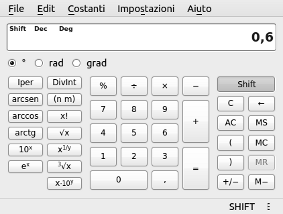
\includegraphics[scale=.65]{/part09/chapG/kcalc.png}
 \caption{Calcolatrice \emph{kcalc}.}\label{fig:G.4}
\end{minipage}
\end{figure}

\emph{Dati}:~$\overline{AB}=5\unit{m}$;\quad~$\overline{AH}=3\unit{m}$. \qquad\emph{Obiettivo}:~$\alpha$.

\begin{soluzione}
 Partiamo dalla formula~$\overline{AH}=\overline{AB}\cdot \cos(\alpha)$, da essa possiamo ottenere
$\cos(\alpha)=\frac{\overline{AH}}{\overline{AB}}$. Sostituendo i valori noti otteniamo
$\cos(\alpha)=\frac{\overline{AH}}{\overline{AB}}=\frac{3}{5}=\np{0,6}$.

Per risalire dal valore del coseno al valore dell'angolo usiamo la calcolatrice attivando la funzione inversa di coseno; su molte calcolatrici
tale funzione è indicata con~$\cos^{-1}$, funzione che si attiva premendo il tasto \emph{Shift} (figura~\ref{fig:G.4}); in \emph{kcalc}
premendo il tasto \emph{Shift} il tasto $cos$ cambia funzionalità e assumendo quella della sua funzione inversa con la scritta \emph{arccos}.

Calcoliamo la misura dell'angolo il cui coseno è~$0,6$ immettendo tale valore nella calcolatrice e attivando i tasti \emph{Shift} e \emph{arccos}.
La calcolatrice restituisce~$53.13010235$.
Questo risultato ci dice che l'angolo è di~$53\grado$ più una parte decimale~$\np{0,13010235}$.
Ricordiamo che i sottomultipli del grado vengono espressi in sessantesimi ($1\grado=60'$ cioè 60 \emph{primi}),
a loro volta suddivisi in sessantesimi ($1'=60''$ cioè 60 \emph{secondi}).
Dunque la parte decimale estratta dalla calcolatrice va adeguatamente modificata:
al risultato della calcolatrice togliamo la parte intera~$(53)$ e moltiplichiamo per~$60$ ottenendo~$\np{7,806141}$ la cui parte
intera (7) rappresenta i \emph{primi}; togliamo nuovamente la parte intera (7) e moltiplichiamo per~$60$ ottenendo i \emph{secondi}~$\np{48,36846}$
Arrotondiamo la parte intera e possiamo concludere~$\alpha\simeq 53\grado 7'48''$.
Alcune calcolatrici scientifiche fanno in automatico questi calcoli attivando un tasto opportuno.

Osserviamo che viene utilizzato il simbolo~$\simeq$ (circa uguale) per indicare che abbiamo usato valori approssimati.
Ora sei in grado di determinare l'ampiezza degli angoli acuti attivando le funzioni inverse sulla tua calcolatrice.
\end{soluzione}

\ovalbox{\risolvii \ref{ese:G.3}, \ref{ese:G.4}, \ref{ese:G.5}}

\section{Operazioni con i gradi sessagesimali}

Accenniamo alle addizioni e sottrazioni tra angoli.

\begin{exrig}
 \begin{esempio}
Svolgiamo l'operazione~$48\grado~45' 52'' + 62\grado~27' 22''$.
\begin{center}
 % (c) 2012 Dimitrios Vrettos - d.vrettos@gmail.com

\begin{tikzpicture}[x=10mm,y=10mm]

\matrix (a) [matrix of nodes,matrix anchor=east] at (0,0){
48$\grado$&45'&52''&$+$\\
62$\grado$&27'&22''&{}\\
110$\grado$&72'&74''&{}\\
111$\grado$&13'&14''&{}\\};

\draw (a-2-1.south west) -- (a-2-4.south east);
\end{tikzpicture}
\end{center}

Sommando termine a termine otteniamo~$110\grado~72' 74''$. Tenendo conto che~1 grado equivale a~60 primi e~1 primo equivale a~60 secondi,
si ha che i~$74\grado$ valgono~$1'$ e~$14''$, i~$72' 74''$ diventano allora~$73'$ e~$14''$.
Trasformiamo poi i~$73'$ in~$1\grado$ e~$13'$.

In definitiva si ha che~$110\grado~72' 74'' = 111\grado~13' 14''$.
 \end{esempio}

 \begin{esempio}
Svolgiamo ora una sottrazione:~$90\grado - 45\grado~33' 12''$.
\begin{center}
 % (c) 2012 Dimitrios Vrettos - d.vrettos@gmail.com

\begin{tikzpicture}[x=10mm,y=10mm]

\matrix (a) [matrix of nodes,matrix anchor=north] at (0,0){
90$\grado$&&&$-$\\
45$\grado$&33'&12''&{}\\};

\draw (a-2-1.south west) -- (a-2-3.south east);

\begin{scope}[xshift=14mm,yshift=-10mm,->, Maroon, thick]
\draw (0,0) -- (.5,0);
\end{scope}

\begin{scope}[xshift=35mm]
\matrix (a) [matrix of nodes,matrix anchor=north] at (0,0){
89$\grado$&59'&60''&$-$\\
45$\grado$&33'&12''&{}\\
44$\grado$&26'&48''&{}\\};

\draw (a-2-1.south west) -- (a-2-3.south east);
\end{scope}
\end{tikzpicture}
\end{center}

Questa è una operazione molto comune, poiché capita abbastanza spesso di dover calcolare l'angolo complementare.
Per svolgere la sottrazione conviene scrivere~$90\grado$ come~$89\grado~59' 60''$ e svolgere la sottrazione avendo come risultato~$44\grado~26' 48''$.
 \end{esempio}

 \begin{esempio}
Un'ultima sottrazione:~$72\grado~20' 40'' - 23\grado~40' 52''$.

Per fare questa sottrazione parto dai secondi e non potendo fare~$40-52$, utilizzo il riporto trasformando~$72\grado~20' 40''$
in~$72\grado~19' 100''$. Ora posso eseguire agevolmente la sottrazione e ottengo~$100-52=48$;
sottraggo poi i primi tra loro, aggiungendo il riporto ai~$19'$ ($72\grado 19' \:\rightarrow\: 71\grado 79'$) e ottengo~$79-40=39$; sottraggo poi i gradi:~$71-23=48$.
Il risultato finale è quindi~$48\grado~39' 48''$.
 \end{esempio}
\end{exrig}

\ovalbox{\risolvi \ref{ese:G.6}}

\section{Risoluzione di triangoli rettangoli}

Ricordiamo che risolvere un triangolo significa ricavare le misure di tutti i suoi elementi (lati e angoli) date le misure di alcuni di essi.

\begin{exrig}
 \begin{esempio}
Determinate l'area del triangolo rettangolo $ABC$, retto in $A$, sapendo che il cateto~${BC}=2\unit{m}$ e che $\widehat{ABC}=\beta=20\grado$.

\emph{Dati}:~$\widehat{BAC}=90\grado$,\quad~$\overline{BC}=2\unit{m}$,\quad~$\widehat{ABC}=\beta=20\grado$.

\emph{Obiettivo}:~$\Area{(ABC)}$.

\emph{Procedura risolutiva}:
$\Area{(ABC)}=\frac{1}{2}\cdot \overline{AB}\cdot \overline{AC}$.

Dobbiamo dunque determinare le misure dei cateti. Applicando le definizioni ($\gamma=\widehat{ACB}$):
\[\overline{AB}=\overline{BC}\cdot {\cos(\beta)}=2\cdot {\cos(20\grado)}\simeq 2\cdot 0,940\simeq 1,879\]
\[\overline{AC}=\overline{BC}\cdot {\cos(\gamma)}=2\cdot {\cos(70\grado)}\simeq 2\cdot 0,342\simeq 0,684\]

Pertanto $\Area\simeq 0,643\unit{(m^{2})}$.
 \end{esempio}

 \begin{esempio}
Un triangolo rettangolo $ABC$, retto in $A$, ha il cateto~$AB$ di~$5\unit{cm}$ e l'angolo acuto in~$C$ di~$57\grado$; determinate l'altro angolo acuto,
la misura del cateto~$AC$ e la misura dell'ipotenusa~$BC$.

\emph{Dati}:~$\widehat{BAC}=90\grado$,\quad~$\widehat{BCA}=57\grado$,\quad~$\overline{AB}=5\unit{cm}$.

\emph{Obiettivo}:~$\beta=\widehat{ABC}$,\quad~$\overline{AC}$,\quad~$\overline{BC}$.

\emph{Procedura risolutiva}:
Essendo gli angoli acuti complementari si ottiene~$\beta=90\grado-57\grado=33\grado$.
Applicando la formula inversa:
\[\overline{CB}=\frac{\overline{AB}}{\cos(\beta)}=\frac{5}{\cos(33\grado)}\simeq \frac{5}{0,839}\simeq 5,962\unit{cm}.\]
Infine determiniamo l'altro cateto e osserviamo che possiamo procedere in due modi:
\begin{itemize*}
 \item con il Teorema di Pitagora:
 \[\overline{CA}=\sqrt{\overline{CB}^{2}-\overline{AB}^{2}}\simeq \sqrt{35,543-25}\simeq \sqrt{10,543}\simeq 3,247\unit{cm};\]
 \item per definizione di coseno:
 \[\overline{CA}=\overline{CB}\cdot \cos(\gamma)\simeq 5,962 \cdot \cos(57\grado)\simeq 5,962\cdot 0,545\simeq 3,247\unit{cm}.\]
\end{itemize*}
\osservazione
\begin{enumeratea}
\item Nei calcoli effettuati abbiamo operato un'approssimazione; per esempio il valore esatto di~$\overline{CB}$ è rappresentato solo
dall'espressione~$\overline{CB}=\frac{\overline{AB}}{\cos(\beta)}=\frac{5}{\cos(33\grado)}$.
\item I risultati ottenuti con procedimenti diversi possono differire, se pur di poco, a causa dell'uso di valori approssimati
nei calcoli che aumentano l'errore di approssimazione (propagazione dell'errore).
\end{enumeratea}
 \end{esempio}

 \begin{esempio}
Risolvi il triangolo rettangolo della figura sapendo che~$c=20\unit{cm}$ e~$\sin(\beta)=\frac{3}{5}$.
\begin{center}
 % (c) 2012 Dimitrios Vrettos - d.vrettos@gmail.com

\begin{tikzpicture}[x=9mm,y=9mm, font=\small]

  \coordinate (A) at (0,0);
  \coordinate (C) at ($(A)+(90:3)$);
  \coordinate (B) at ($(A)+(0:4)$);

  \draw (A) node[below left]{$A$}-- (C) node[above left]{$C$} -- (B)node[below right]{$B$} -- (A);

  \tkzMarkAngle[ fill=LimeGreen ,draw, size=.4](A,C,B)
  \tkzMarkAngle[ fill=LimeGreen ,draw, size=.4](C,B,A)
  \tkzMarkRightAngle[ fill=LimeGreen ,draw, size=.3](C,A,B)
  
  \begin{scope}[font=\scriptsize]
    \tkzLabelAngle[pos=.6](A,C,B){$\gamma$}
    \tkzLabelAngle[pos=.6](C,B,A){$\beta$}
    \tkzLabelAngle[pos=.6](C,A,B){$\alpha$}
  \end{scope}

  \tkzLabelSegment[midway, left](A,C){$b$}
  \tkzLabelSegment[midway, below](A,B){$c$}
  \tkzLabelSegment[midway, above](B,C){$a$}

  \begin{scope}[fill=CornflowerBlue, draw=black]
    \filldraw (0,0) circle (1pt);
    \filldraw (4,0) circle (1pt);
    \filldraw (0,3) circle (1pt);
  \end{scope}

\end{tikzpicture}
\end{center}
Usiamo l'identità fondamentale per determinare~$\cos(\beta)$:
\[\cos(\beta)=\sqrt{1-\sin^{2}(\beta)}=\sqrt{1-\left(\frac{3}{5}\right)^{2}}=\sqrt{1-\frac{9}{25}}=
    \sqrt{\frac{25-9}{25}}=\sqrt{\frac{16}{25}}=\frac{4}{5};\]

Poiché $\cos(\beta)=\dfrac{c}{a}$ si ha:
\[a=\frac{c}{\cos(\beta)}=\frac{20}{\frac{4}{5}}=\frac{20\cdot{5}}{4}=25\unit{cm}.\]

Per il teorema di Pitagora~$b=\sqrt{a^{2}-c^{2}}=\sqrt{25^{2}-20^{2}}=15\unit{cm}$;

$\beta\simeq 36\grado~52' 12''$ (calcolato con la calcolatrice e arrotondato), $\gamma = 90\grado - \beta \simeq 53\grado~07'48''$.
 \end{esempio}

 \begin{esempio}
Risolvere il triangolo rettangolo~$ABC$, retto in~$A$ (quello della figura precedente) sapendo che~$b=2\unit{cm}$ e~$\sin(\beta)=0,2$.

\emph{Dati}:~$b=2\unit{cm}$,\quad~$\sin(\beta)=0,2$.

\emph{Obiettivo}:~$a$,\quad~$c$,\quad~${\beta}$,\quad~${\gamma}$.

\emph{Procedura risolutiva}:
Dalle definizione di seno $\sin(\beta)=\dfrac{b}{a}$ si ha
\[a=\frac{b}{\sin(\beta)}=\frac{2}{0,2}=10\unit{cm}.\]
Con il teorema di Pitagora possiamo ricavare l'altro cateto
\[c=\sqrt{a^{2}-b^{2}}=\sqrt{100-4}=\sqrt{96}=4\sqrt{6}\simeq 9,798\unit{cm}.\]
Infine, con la funzione inversa, ricaviamo l'angolo~${\beta}=\sin^{-1}(0,2)\simeq 11,537$ e procedendo come spiegato in
precedenza otteniamo:~${\beta}\simeq 11\grado~32' 13''$ e~${\gamma}=90\grado-\beta\simeq 78\grado~27'47''$.
 \end{esempio}
\end{exrig}

\ovalbox{\risolvii \ref{ese:G.7}, \ref{ese:G.8}, \ref{ese:G.9}, \ref{ese:G.10}}

\subsection{Proiezione di un segmento lungo una direzione}

\begin{definizione}
Dato un segmento~$AB$ ed una retta~$r$ che passa per un suo estremo ($A$, per fissare le idee). Si definisce
\emph{proiezione del segmento $AB$ sulla retta $r$} il segmento~$AH$ dove~$H$ è l'intersezione fra~$r$ e la
sua perpendicolare passante per~$B$ (si vedano i tre esempi riportati nella figura seguente).
\end{definizione}

\begin{center}
 % (c) 2012 Dimitrios Vrettos - d.vrettos@gmail.com

\begin{tikzpicture}[x=10mm,y=10mm, font=\small]

  \coordinate (A) at (0,0);
  \coordinate (H) at ($(A)+(0:3)$);
  \coordinate (B) at ($(H)+(90:2)$);

  \draw (B)node[above right]{$B$} -- (A) node[below]{$A$}-- (H) node[below]{$H$};
  \draw[dashed] (B)--(H);

  \draw (-.5,0) -- (3.5,0)node[below] {$r$};
  \tkzMarkAngle[ fill=LimeGreen ,draw, size=.4](H,A,B)

  \begin{scope}[font=\scriptsize]
    \tkzLabelAngle[pos=.6](H,A,B){$\alpha$}
  \end{scope}

  \begin{scope}[fill=CornflowerBlue, draw=black]
    \filldraw (0,0) circle (1pt);
    \filldraw (3,0) circle (1pt);
    \filldraw (3,2) circle (1pt);
  \end{scope}

  \begin{scope}[xshift=45mm]
    \tkzDefPoints{0/1/A, 2/0/B,1.25/1.59/H}
    \tkzDrawLine[add=0 and 0, dashed, thin](B,H)
    \tkzDrawLine[add=0 and 0,thin](A,B)
    \tkzMarkAngle[fill=LimeGreen ,draw, size=.4](B,A,H) 
    \tkzDrawLine[add = .4 and .4, end=$r$, thin](A,H)

    \tkzLabelPoint[above](H){$H$}
    \tkzLabelPoint[above](A){$A$}
    \tkzLabelPoint[below](B){$B$}
    
    \begin{scope}[font=\scriptsize]
      \tkzLabelAngle[pos=.6](H,A,B){$\alpha$}
    \end{scope}
    
    \tkzDrawPoints[fill=CornflowerBlue](A,B, H)
  \end{scope}

  \begin{scope}[xshift=80mm, rotate=-10]
    \tkzDefPoints{0/0/A, 0/2/H, 2/2/B}
    \tkzDrawLine[add=0 and 0, dashed, thin](B,H)
    \tkzDrawLine[add=0 and 0,thin](A,B)
    \tkzDrawLine[add = 0 and .2, end=$r$, thin](A,H)

    \tkzLabelPoint[left](H){$H$}
    \tkzLabelPoint[below](A){$A$}
    \tkzLabelPoint[right](B){$B$}
    \tkzMarkAngle[fill=LimeGreen ,draw, size=.4](B,A,H) 

  \begin{scope}[font=\scriptsize]
    \tkzLabelAngle[pos=.6](H,A,B){$\alpha$}
  \end{scope}
    \tkzDrawPoints[fill=CornflowerBlue](A,B, H)
  \end{scope}
\end{tikzpicture}
\end{center}

\ovalbox{\risolvii \ref{ese:G.11}, \ref{ese:G.12}, \ref{ese:G.13}, \ref{ese:G.14}, \ref{ese:G.15}, \ref{ese:G.16}, \ref{ese:G.17}, \ref{ese:G.18},
\ref{ese:G.19}, \ref{ese:G.20}, \ref{ese:G.21}}

\section{Risoluzione di un triangolo qualsiasi con triangoli rettangoli}
Per risolvere i triangoli qualsiasi, tramite l'altezza, bisogna ricercare all'interno della figura considerata dei triangoli rettangoli.
Nel seguito saranno indicati altri teoremi che permettono
di risolvere tutti i tipi di triangoli.

\begin{figure}[b]
\begin{minipage}[t]{.45\textwidth}
 \centering
 % (c) 2012 Dimitrios Vrettos - d.vrettos@gmail.com

\begin{tikzpicture}[x=10mm,y=10mm, font=\small]

  \coordinate (A) at (0,0);
  \coordinate (B) at ($(A)+(0:4.18)$);
  \coordinate (C) at ($(A)+(39:3.5)$);
  \coordinate (H) at ($(A)+(0:2.72)$);

  \draw (B) node[below right]{$B$}--(A) node[below left]{$A$}--(C) node[above]{$C$}--(B);

  \tkzMarkAngle[ fill=LimeGreen ,draw, size=.4](H,A,C)
  \tkzMarkAngle[ fill=LimeGreen ,draw, size=.4](A,C,B)
  \tkzMarkAngle[ fill=LimeGreen ,draw, size=.4](C,B,H)

  \draw (C)--(H) node[below]{$H$};

  \begin{scope}[font=\scriptsize]
    \tkzLabelAngle[pos=.6](H,A,C){$\alpha$}
    \tkzLabelAngle[left, pos=.6](A,C,B){$\gamma$}
    \tkzLabelAngle[pos=.6](C,B,H){$\beta$}
  \end{scope}
  
  \begin{scope}[fill=CornflowerBlue, draw=black]
    \filldraw (0,0) circle (1pt);
    \filldraw (4.18,0) circle (1pt);
    \filldraw (2.72,2.2) circle (1pt);
    \filldraw (2.72,0) circle (1pt);
  \end{scope}
\end{tikzpicture}
 \caption{Triangolo acutangolo.}\label{fig:G.5}
\end{minipage}\hfil
\begin{minipage}[t]{.45\textwidth}
\centering
 % (c) 2012 Dimitrios Vrettos - d.vrettos@gmail.com

\begin{tikzpicture}[x=10mm,y=10mm, font=\small]

  \coordinate (A) at (0,0);
  \coordinate (B) at ($(A)+(0:4.26)$);
  \coordinate (C) at ($(B)+(145:3.486)$);
  \coordinate (D) at ($(A)+(90:2)$);

  \draw (D) node[above left]{$D$}--(A) node[below left]{$A$}--(B) node[below right]{$B$}--(C)node [above right]{$C$} --(D);

  \tkzMarkAngle[ fill=LimeGreen ,draw, size=.4](C,A,D)
  \tkzMarkAngle[ fill=LimeGreen ,draw, size=.4](A,C,B)
  \tkzMarkAngle[ fill=LimeGreen ,draw, size=.4](C,B,A)

  \draw[dashed] (C)--(A);

  \begin{scope}[fill=CornflowerBlue, draw=black]
    \filldraw (0,0) circle (1pt);
    \filldraw (4.26,0) circle (1pt);
    \filldraw (1.4,2) circle (1pt);
    \filldraw (0,2) circle (1pt);
  \end{scope}
\end{tikzpicture}
\caption{Trapezio rettangolo.}\label{fig:G.6}
\end{minipage}
 \end{figure}

\begin{exrig}
 \begin{esempio}
Risolvi il triangolo acutangolo della figura~\ref{fig:G.5} con~$\alpha=39\grado$, $\beta=57\grado$ e $\overline{CH}=11\unit{m}$.

Ricordando che la somma degli angoli di un triangolo è~$180\grado$ ricaviamo~$\gamma$:
\[ \gamma =180\grado-\alpha -\beta =180\grado-39\grado-57\grado=84\grado.\]

Individuiamo ora i triangoli rettangoli nella figura in modo da poter applicare le formule.

Con il triangolo rettangolo~$CHB$:
\begin{align*}
 &\sin(\beta)=\frac{\overline{CH}}{\overline{CB}} \quad\Rightarrow\quad \overline{CB}=\frac{\overline{CH}}{\sin(\beta)}=
    \frac{11}{\sin(57\grado)}\simeq \np[m]{13,2};\\
&\tan(\beta)=\frac{\overline{CH}}{\overline{BH}} \quad\Rightarrow\quad \overline{BH}=\frac{\overline{CH}}{\tan(\beta)}=
    \frac{11}{\tan(57\grado)}\simeq \np[m]{7,15}.
\end{align*}

Con il triangolo rettangolo~$AHC$:
\begin{align*}
&\sin(\alpha)=\frac{\overline{CH}}{\overline{AC}} \quad\Rightarrow\quad \overline{AC}=\frac{\overline{CH}}{\sin(\alpha)}=
    \frac{11}{\sin(39\grado)}\simeq \np[m]{17,46};\\
&\tan(\alpha)=\frac{\overline{CH}}{\overline{AH}} \quad\Rightarrow\quad \overline{AH}=\frac{\overline{CH}}{\tan(\beta)}=
    \frac{11}{\tan(39\grado)}\simeq \np[m]{13,75}.
\end{align*}

Infine calcoliamo~$\overline{AB}=\overline{AH}+\overline{BH}\simeq \np{7,15}+\np{13,75} = \np{20,9}\unit{m}$.
 \end{esempio}
\end{exrig}

\ovalbox{\risolvii \ref{ese:G.22}, \ref{ese:G.23}, \ref{ese:G.24}, \ref{ese:G.25}}

\subsection{Quadrilateri}

\begin{exrig}\vspace{1.10ex}
 \begin{esempio}
Nel trapezio rettangolo~$ABCD$ della figura~\ref{fig:G.6} il lato obliquo~$BC$ forma un angolo di~$35\grado$ con la base maggiore~$AB$, inoltre la diagonale~$AC$
è perpendicolare a~$BC$. Calcola il perimetro e l'area del trapezio sapendo che la sua altezza è~$10\unit{cm}$.

Ricordando che la somma degli angoli di un triangolo è~$180\grado$ ricaviamo~$\widehat{CAB}=55\grado$.
Siccome il trapezio è rettangolo
$\widehat{DAC}=\widehat{DAB}-\widehat{CAB}=90\grado-55\grado$.
Calcoliamo ora~$CB$, $AB$ e~$DC$:
\begin{align*}
&\sin(\widehat{ABC})=\frac{\overline{AD}}{\overline{CB}} \quad\Rightarrow\quad
    \overline{CB}=\frac{\overline{AD}}{\sin(\widehat{ABC})}=\frac{10}{\sin(35\grado)}\simeq \np[cm]{17,43};\\
&\overline{AB}=\frac{\overline{CB}}{\cos(\widehat{ABC})}\simeq \frac{\np{17,43}}{\cos(55\grado)}\simeq \np[cm]{21,28};\\
&\frac{\overline{DC}}{\overline{AD}}=\tan(\widehat{DAC}) \quad\Rightarrow\quad \overline{DC}=\overline{AD}\cdot\tan(\widehat{DAC})=10\tan(35\grado)\simeq \np{7,00}.
\end{align*}

Da cui:
\begin{align*}
&2p=\overline{AB}+\overline{BC}+\overline{DC}+\overline{DA}\simeq \np{21,28}+\np{17,43}+\np{7,00}+10 = \np[cm]{55,71};\\
&\Area=\frac{(\overline{AB}+\overline{DC})\cdot\overline{AD}}{2}\simeq \frac{(\np{21,28}+\np{7,00})\cdot 10}{2}\simeq \np[cm^2]{141,40}.
\end{align*}
 \end{esempio}
\end{exrig}

\ovalbox{\risolvii \ref{ese:G.26}, \ref{ese:G.27}, \ref{ese:G.28}, \ref{ese:G.29},\ref{ese:G.30}, \ref{ese:G.31}, \ref{ese:G.32}, \ref{ese:G.33}}

\subsection{Applicazioni alla topografia}

La topografia è una disciplina che studia gli strumenti ed i metodi operativi, sia di calcolo che di disegno, necessari per ottenere
una rappresentazione grafica di una parte della superficie terrestre.
La topografia ha carattere applicativo e trae la sua base teorica dalla matematica, dalla geometria e dalla trigonometria.

\begin{exrig}
 \begin{esempio}
Risolvere il quadrilatero della figura~\ref{fig:G.7} sapendo che~$AB=\np[m]{42,5}$, $BC=\np[m]{32,18}$, $CD=\np[m]{27,6}$,
$\widehat{BAD}=56\grado$, $\widehat{ADC}=62\grado$.

\begin{figure}[ht]
\centering
% (c) 2012 Dimitrios Vrettos - d.vrettos@gmail.com

\begin{tikzpicture}[x=10mm,y=10mm, font=\small]

\coordinate (A) at (0,0);
\coordinate (D) at ($(A)+(0:6.702)$);
\coordinate (B) at ($(A)+(56:4.25)$);
\coordinate (C) at ($(D)+(118:2.76)$);
\coordinate (F) at ($(A)+(0:2.38)$);
\coordinate (G) at ($(F)+(90:2.43)$);
\coordinate (E) at ($(A)+(0:5.4)$);

\draw (B) node[above]{$B$}--(A) node[below left]{$A$}--(D) node[below right]{$D$}--(C)node [right]{$C$} --(B);

\tkzMarkAngle[ fill=LimeGreen ,draw, size=.4](D,A,B)
\tkzMarkAngle[ fill=LimeGreen ,draw, size=.4](C,D,A)

\begin{scope}[dashed]
\draw(B)--(F) node[below]{$F$};
\draw(C)--(G)node[left]{$G$};
\draw(C)--(E)node[below]{$E$};
\end{scope}

\begin{scope}[fill=CornflowerBlue, draw=black]
\filldraw (0,0) circle (1pt);
\filldraw (6.702,0) circle (1pt);
\filldraw (5.4,2.43) circle (1pt);
\filldraw (2.38,3.52) circle (1pt);
\filldraw (2.38,0) circle (1pt);
\filldraw (2.38,2.43) circle (1pt);
\filldraw (5.4,0) circle (1pt);
\end{scope}
\end{tikzpicture}
\caption{Il quadrilatero~$ABCD$.}\label{fig:G.7}
\end{figure}

\emph{Dati}:~$\overline{AB}=\np[m]{42,5}$,\quad~$\overline{BC}=\np[m]{32,18}$,\quad~$\overline{CD}=\np[m]{27,6}$,\quad~$\widehat{BAD}=56\grado$,\quad~$\widehat{ADC}=62\grado$.

\emph{Obiettivo}:~$\overline{AD}$,\quad~$\widehat{ABC}$,\quad~$\widehat{CDA}$.

\emph{Procedura risolutiva}:
Suddividiamo il quadrilatero in tre triangoli rettangoli e in un rettangolo, come nella figura, e risolviamo i triangoli.

Triangolo~$FBA$ retto in $F$:
\begin{align*}
&\widehat{FBA}=90\grado-\widehat{BAD}=90\grado-56\grado=34\grado;\\
&\overline{AF}=\overline{AB}\cos(\widehat{BAD})=\np{42,5}\cos(56\grado)\simeq \np[m]{23,77};\\
&\overline{BF}=\overline{AB}\sin(\widehat{BAD})=\np{42,5}\sin(56\grado)\simeq \np[m]{35,23}.
\end{align*}

Triangolo~$DCE$ retto in $E$:
\begin{align*}
&\widehat{DCE}=90\grado-\widehat{ADC}=90\grado-62\grado=28\grado;\\
&\overline{DE}=\overline{CD}\cos(\widehat{FBA})=\np{27,6}\cos(62\grado)\simeq \np[m]{12,96};\\
&\overline{CE}=\overline{CD}\sin(\widehat{ADC})=\np{27,6}\sin(62\grado)\simeq \np[m]{24,37}.
\end{align*}

Triangolo~$GBC$ retto in $G$:
\begin{align*}
&\overline{BG}=\overline{BF}-\overline{GF}=\overline{BF}-\overline{CE}\simeq \np{35,23}-\np{24,37}\simeq \np[m]{10,86};\\
&\cos(\widehat{CBG})=\frac{\overline{BG}}{\overline{BC}}\simeq \frac{\np{10,86}}{\np{32,18}}\simeq \np{0,34}\:\Rightarrow\: \widehat{CBG}=\cos^-1(\np{0,34})\simeq 70\grado~16' 36'';\\
&\widehat{BCG}=90\grado-\widehat{CBG}\simeq 90\grado-70\grado~16' 36''\simeq 19\grado~43' 24'';\\
&\overline{GC}=\overline{BC}\sin(\widehat{CBG})\simeq \overline{BC}\sin(70\grado~16' 36'')\simeq \np[m]{30,29}.
\end{align*}

Calcoliamo ora gli elementi incogniti del quadrilatero:
\begin{align*}
&\overline{DA}=\overline{AF}+\overline{FE}+\overline{ED}\simeq \np{23,77}+\np{30,29}+\np{12,96} = \np[m]{67,02};\\
&\widehat{ABC}=\widehat{ABF}+\widehat{FBC}\simeq 34\grado+70\grado~16' 36'' = 104\grado~16' 36'';\\
&\widehat{BCD}= \widehat{BCG}+\widehat{GCE}+\widehat{ECD}\simeq 19\grado~43' 24''+90\grado+34\grado = 143\grado~43' 24''.
\end{align*}
\end{esempio}
\end{exrig}

\ovalbox{\risolvii \ref{ese:G.34}, \ref{ese:G.35}, \ref{ese:G.36}, \ref{ese:G.37}, \ref{ese:G.38}, \ref{ese:G.39}, \ref{ese:G.40}, \ref{ese:G.41}, \ref{ese:G.42}}

\vspazio\ovalbox{\ref{ese:G.43}, \ref{ese:G.44}, \ref{ese:G.45}, \ref{ese:G.46}}

\section{Risoluzione di un triangolo qualunque}

Le funzioni trigonometriche possono essere calcolate anche su angoli maggiori di~$90\grado$. Poiché, al momento, siamo interessati alle
applicazioni sui triangoli, ci basterà estendere le nostre considerazioni agli angoli compresi fra~$90\grado$ e~$180\grado$,
essendo~$180\grado$ la misura limite superiore di un angolo interno di un triangolo.
\begin{exrig}
 \begin{esempio}
Analizziamo la tabella con i valori approssimati alla quarta cifra decimale delle funzioni seno e coseno per alcuni angoli da~$0\grado$ a~$180\grado$.
\[
\begin{array}{cccccccccccc}
\toprule
\alpha&0\grado &30\grado &45\grado &60\grado &90\grado & 120\grado & 135\grado &150\grado &180\grado\\
\midrule
\sin(\alpha)& 0 & \np{0,5} & \np{0,7071} & \np{0,8660} & 1 & \np{0,8660} & \np{0,7071} & \np{0,5} & 0\\
\cos(\alpha)& 1 & \np{0,8660} & \np{0,7071} & \np{0,5} & 0 & \np{-0,5} & \np{-0,7071} & \np{-0,8660} &-1\\
\bottomrule
\end{array}
\]
Dalla tabella si nota che la funzione seno si mantiene positiva nell'intervallo ($0\grado$, $180\grado$), nei cui estremi si annulla.
Inoltre essa assume il valore massimo, uguale a~1, quando l'angolo è di~$90\grado$.
La funzione coseno, invece, è negativa per angoli compresi tra~$90\grado$ e~$180\grado$. Più precisamente essa decresce da~$1$ a~$0$
man mano che l'angolo su cui è calcolata cresce da~$0\grado$ a~$90\grado$, si annulla quando l'angolo è esattamente~$90\grado$, dopodiché continua a decrescere, da~$0$ a~$-1$ man mano che l'angolo passa da~$90\grado$ a~$180\grado$.
Osserviamo anche che angoli supplementari (la cui somma è l'angolo piatto, cioè~$180\grado$) hanno lo stesso seno ma coseno opposto.
Queste considerazioni saranno chiarite con lo studio delle funzioni circolari.
 \end{esempio}
\end{exrig}
Affrontiamo ora il problema della risoluzione di un triangolo qualsiasi.
Come sappiamo, gli elementi caratteristici di un triangolo sono le misure dei suoi lati e dei suoi angoli.
Sappiamo anche che per determinare univocamente un triangolo sono, in linea di massima, necessari solo tre di questi elementi
purché uno almeno di questi sia un lato. Ciò deriva dai tre criteri di \emph{congruenza} dei triangoli che andiamo a ricordare.

\paragraph{Primo criterio di congruenza} Due triangoli che abbiano rispettivamente congruenti due lati e l'angolo tra essi
compreso sono congruenti.

\paragraph{Secondo criterio di congruenza}
Due triangoli che abbiano rispettivamente congruenti un lato e due
angoli ugualmente posti rispetto al lato sono congruenti.

\paragraph{Terzo criterio di congruenza}
Due triangoli che abbiano rispettivamente congruenti i tre lati sono congruenti.
\\

Ricordiamo che due triangoli che abbiano ordinatamente uguali tutti gli angoli non sono, in generale, congruenti, bensì sono \emph{simili}.

Quello che ci chiediamo è se la trigonometria, finora usata solo per i triangoli rettangoli, ci possa venire in aiuto per la
determinazione delle misure degli elementi incogniti di un triangolo qualunque, quando conosciamo i tre elementi che lo
determinano univocamente. Ad esempio, se è assegnata la lunghezza di due lati e l'ampiezza dell'angolo compreso,
la geometria euclidea ci aiuta a costruire il suddetto triangolo tramite riga e compasso ma non ci dice nulla delle
misure degli elementi incogniti.

Disegniamo un triangolo avendo cura di indicare con la stessa lettera vertice e lato opposto e di nominare con
$\alpha$, $\beta$ e $\gamma$ le ampiezze degli angoli di vertice rispettivamente~$A$, $B$ e $C$.
\begin{center}
 % (c) 2012 Dimitrios Vrettos - d.vrettos@gmail.com

\begin{tikzpicture}[x=10mm,y=10mm, font=\small]

\coordinate (A) at (0,0);
\coordinate (B) at ($(A)+(40:4)$);
\coordinate (C) at ($(A)+(0:2.5)$);

\draw (A) node[below left]{$A$}--(B) node[above]{$B$}--(C)node [below right]{$C$} --(A);

\tkzMarkAngle[ fill=LimeGreen ,draw, size=.4](C,A,B)
\tkzMarkAngle[ fill=LimeGreen ,draw, size=.4](A,B,C)
\tkzMarkAngle[ fill=LimeGreen ,draw, size=.4](B,C,A)

\tkzLabelSegment[midway, below](A,C){$b$}
\tkzLabelSegment[midway, above](A,B){$c$}
\tkzLabelSegment[midway, right](B,C){$a$}

\begin{scope}[font=\scriptsize]
\tkzLabelAngle[pos=.6](C,A,B){$\alpha$}
\tkzLabelAngle[pos=.6](A,B,C){$\beta$}
\tkzLabelAngle[pos=.6](B,C,A){$\gamma$}
\end{scope}

\begin{scope}[fill=CornflowerBlue, draw=black]
\filldraw (0,0) circle (1pt);
\filldraw (2.5,0) circle (1pt);
\filldraw (3.05,2.55) circle (1pt);
\end{scope}
\end{tikzpicture}
\end{center}

\subsection{Caso I: due lati e l'angolo compreso congruenti}

Come abbiamo premesso, assegnati due lati e l'angolo tra essi compreso, la geometria euclidea ci assicura l'esistenza
di un solo triangolo che soddisfi i dati, ma non ci permette di determinare la misura del terzo lato, né le ampiezze degli altri angoli.
Abbiamo bisogno di altri strumenti come il teorema di Carnot.\footnote{dal nome del fisico, ingegnere e matematico francese (1796 - 1832), anche se il teorema è dovuto al matematico e politico francese François Viète (1540 - 1603).}

\begin{teorema}[del coseno o di Carnot]
In un triangolo qualsiasi di cui siano note le lunghezze di due lati e l'ampiezza dell'angolo compreso, il quadrato della lunghezza
del lato incognito è uguale alla somma dei quadrati delle lunghezze note diminuita del loro doppio prodotto per il coseno dell'angolo compreso.

A seconda di quali siano i due lati noti, traducendo in linguaggio matematico quanto afferma l'enunciato si ha:
\begin{align*}
&c^{2}=a^{2}+b^{2}-2\cdot a\cdot b\cdot \cos(\gamma);\\
&a^{2}=b^{2}+c^{2}-2\cdot b\cdot c\cdot \cos(\alpha);\\
&b^{2}=a^{2}+c^{2}-2\cdot a\cdot c\cdot \cos(\beta).
\end{align*}
\end{teorema}

\begin{problema}
Risolvete il triangolo~$ABC$ dati~$a= 20\unit{cm}$, $b=10\unit{cm}$ e $\gamma=36\grado$.
\end{problema}

\emph{Dati}:~$a=20\unit{cm}$,\quad~$b=10\unit{cm}$,\quad~$\gamma=36\grado$.

\emph{Obiettivo}:~$c$,\quad~$\alpha$,\quad~$\beta$.

\emph{Procedura risolutiva}:
per il teorema di Carnot possiamo scrivere
\begin{align*}
&c^{2}=a^{2}+b^{2}-2\cdot a\cdot b\cdot \cos (\gamma)\\
\Rightarrow\quad &c^{2}=20^{2}+10^{2}-2\cdot 20\cdot 10\cdot \cos(36\grado)\simeq 400+100-400\cdot \np{0,809}\simeq \np{176,4}\\
\Rightarrow\quad &c\simeq \sqrt{\np{176,4}}\simeq \np[cm]{13,281}.
\end{align*}

Ora dobbiamo determinare gli altri due angoli; utilizzando ancora il teorema di Carnot ricaviamo $\alpha$
\[a^{2}=b^{2}+c^{2}-2\cdot b\cdot c\cdot \cos(\alpha) \quad\Rightarrow\quad \cos(\alpha)= \dfrac{b^2+c^2-a^2}{2bc}\]
conoscendo $a$, $b$ e $c$ rimane come incognita $\cos(\alpha)$. Sostituiamo i valori noti:
\[\cos(\alpha)\simeq \dfrac{10^2+\np{176,4}-20^2}{2\cdot 10 \cdot \np{13,281}}\simeq\frac{\np{276,4}-400}{\np{265,62}}\simeq\np{-0,4653}\]
da cui
\[\alpha\simeq \cos^{-1}(\np{-0,4653})\simeq 117\grado \quad\Rightarrow\quad \beta = 180\grado - \alpha -\gamma \simeq 180\grado -117\grado - 36\grado \simeq 27\grado\]

Il triangolo è ottusangolo, i suoi lati misurano rispettivamente
$a=20\unit{cm}$, $b=10\unit{cm}$ e $c\simeq \np[cm]{13,2815}$; i suoi angoli hanno ampiezza~$\alpha\simeq 117\grado$, $\beta\simeq 27\grado$ e $\gamma=36\grado$.

\subsection{Caso II: tre lati congruenti}

Sappiamo dalla geometria euclidea che assegnati tre segmenti affinché si possa costruire il triangolo che li ha come lati
deve essere verificato il teorema della disuguaglianza triangolare: ``in qualsiasi triangolo, ogni lato deve essere minore della somma
degli altri due e maggiore della loro differenza''.

\begin{problema}
Determinate le ampiezze degli angoli di un triangolo note le misure dei suoi lati~$a=5\unit{m}$, $b=12\unit{m}$, $c=13\unit{m}$.
\end{problema}

\emph{Dati}:~$a= 5\unit{m}$,\quad~$b=12\unit{m}$,\quad~$c=13\unit{m}$.

\emph{Obiettivo}:~$\alpha$,\quad~$\beta$,\quad~$\gamma$.

\emph{Procedura risolutiva}:
utilizziamo almeno due volte il teorema del coseno per determinare due angoli. Per trovare~$\cos(\gamma)$ utilizziamo
\[c^{2}=a^{2}+b^{2}-2\cdot a\cdot b\cdot \cos(\gamma) \quad\Rightarrow\quad \cos(\gamma) = \dfrac{a^{2}+b^{2}-c^{2}}{2ab}\]
sostituendo i dati si ottiene
\[\cos(\gamma)=\dfrac{5^2+12^2-13^2}{2\cdot 5 \cdot 12}=\dfrac{25+144-169}{120}=0 \quad\Rightarrow\quad \gamma=\cos^{-1}(0)=90\grado.\]
Per trovare~$\cos(\alpha)$ utilizziamo ancora il teorema di Carnot nella formula
\[a^{2}=b^{2}+c^{2}-2\cdot b\cdot c\cdot \cos(\alpha) \quad\Rightarrow\quad \cos(\alpha) = \dfrac{b^{2}+c^{2}-a^{2}}{2bc}\]
sostituendo i valori noti si ottiene
\[\cos(\alpha)=\dfrac{12^2+13^3-5^2}{1\cdot 13\cdot 13}=\frac{169+144-25}{312}\simeq \np{0,9230}\quad\Rightarrow\quad \alpha\simeq\cos^{-1}(\np{0,9230})\simeq 22\grado.\]

Quindi~$\alpha\simeq 22\grado$, $\gamma=90\grado$ e $\beta=180\grado-\alpha-\gamma\simeq 180\grado-90\grado-22\grado\simeq 68\grado$.

\subsection{Caso III: un lato e gli angoli congruenti}

Occorre un altro teorema per il problema della risoluzione di un triangolo qualunque.

\begin{teorema}[dei seni o di Eulero]
In qualsiasi triangolo risulta costante il rapporto fra la lunghezza di un lato e il seno dell'angolo che gli è opposto. In formule:
\[\frac{a}{\sin(\alpha)}=\frac{b}{\sin(\beta)}=\frac{c}{\sin(\gamma)}.\]
\end{teorema}

\begin{problema}
Risolvete il triangolo~$ABC$ sapendo che~$a= \np[m]{7,52}$, $\beta=98\grado$ e $\gamma=27\grado$.
\end{problema}

\emph{Dati}:~$a= \np[m]{7,52}$,\quad~$\beta=98\grado$,\quad~$\gamma=27\grado$.

\emph{Obiettivo}:~$b$,\quad~$c$,\quad~$\alpha$.

\emph{Procedura risolutiva}:
Possiamo immediatamente determinare il terzo angolo: \[\alpha=180\grado-\beta-\gamma=180\grado-98\grado-27\grado=55\grado.\]

Per determinare i lati~$b$ e~$c$ applichiamo il teorema di Eulero.

Per la prima uguaglianza del teorema otteniamo:
\[
\frac{7,52}{\sin(55\grado)}=\frac{b}{\sin(98\grado)} \quad\Rightarrow\quad b=\frac{\np{7,52}}{\sin(55\grado)}\cdot \sin(98\grado)\simeq
\frac{\np{7,52}}{\np{0,8192}}\cdot \np{0,9902}\simeq\np[m]{9,0897}.
\]
Considerando l'uguaglianza tra il primo e l'ultimo rapporto del teorema otteniamo:
\[
\frac{\np{7,52}}{\sin(55\grado)}=\frac{c}{\sin(27\grado)} \quad\Rightarrow\quad c=\frac{\np{7,52}}{\sin(55\grado)}\cdot \sin(27\grado)\simeq\np[m]{4,1674}.
\]

\subsection{Riflessioni sull'uso del teorema dei seni}

\begin{problema}
Risolvete il triangolo~$ABC$ sapendo che~$a= 20\unit{cm}$, $c= 13\unit{cm}$ e $\gamma=36\grado$.
\end{problema}

\emph{Dati}:~$a=20\unit{cm}$,\quad~$c=13\unit{cm}$,\quad~$\gamma=36\grado$.

\emph{Obiettivo}:~$b$,\quad~$\alpha$,\quad~$\beta$.

Gli elementi noti non rispecchiano nessuna delle le condizioni sufficienti espresse dai criteri di congruenza, ma possiamo usare il teorema dei seni
che ci assicura che in qualunque triangolo si ha
 \[\frac{a}{\sin(\alpha)}=\frac{b}{\sin(\beta)}=\frac{c}{\sin(\gamma)}\]
e quindi
\[\frac{20}{\sin(\alpha)}=\frac{13}{\sin(36\grado)}\quad\Rightarrow\quad\sin(\alpha)=\frac{20\cdot\sin(36\grado)}{13}\simeq \np{0,9043}\]
e dunque con la funzione inversa~$\sin^{-1}(\np{0,9043})$ possiamo ricavare l'angolo~$\alpha\simeq 64\grado$. Di conseguenza~$\beta\simeq 80\grado$.

Sembrerebbe tutto corretto, ma abbiamo trascurato il fatto che angoli supplementari hanno lo stesso seno dunque
da~$\sin ^{-1}(\np{0,9043})$ si può ottenere~$\alpha\simeq 64\grado$ oppure~$\alpha\simeq 116\grado$
quindi il triangolo non è univocamente determinato. Proseguendo nel ragionamento avremmo:

\paragraph{Caso I}
$\alpha\simeq 64\grado$, quindi il triangolo è acutangolo e~$\beta\simeq 80\grado$; possiamo determinare~$b$ applicando nuovamente
il teorema dei seni
\[\frac{13}{\sin(36\grado)}=\frac{b}{\sin(80\grado)}\quad\Rightarrow\quad b\simeq \frac{13\cdot\np{0,9848}}{\np{0,5877}}\simeq 21\unit{cm}.\]

\paragraph{Caso II}
$\alpha\simeq 116\grado$, quindi il triangolo è ottusangolo e~$\beta\simeq 28\grado$; possiamo determinare~$b$ con
il teorema dei seni
\[\frac{13}{\sin(36\grado)}=\frac{b}{\sin(28\grado)}\quad\Rightarrow\quad b\simeq \frac{13\cdot\np{0,4694}}{\np{0,5877}}\simeq 10\unit{cm}.\]

Il problema ha pertanto due soluzioni.

\begin{problema}
Risolvete il triangolo~$ABC$ sapendo che~$a= 26\unit{m}$, $b= 12\unit{m}$, $\alpha=124\grado$.
\end{problema}

\emph{Dati}:~$a= 26\unit{m}$,\quad~$b= 12\unit{m}$,\quad~$\alpha=124\grado$.

\emph{Obiettivo}:~$c$,\quad~$\beta$,\quad~$\gamma$.

Applichiamo il teorema dei seni:
\[\frac{13}{\sin(124\grado)}=\frac{12}{\sin(\beta)}\quad\Rightarrow\quad \sin(\beta)=\frac{12\cdot\sin(124\grado)}{26}\simeq\ldots \ldots \ldots.\]
In questo caso non ci sono dubbi: un triangolo non può avere due angoli ottusi. Potete completare voi la soluzione e otterrete
$\beta\simeq \ldots\ldots$ quindi~$\gamma\simeq \ldots\ldots$ e infine~$c\simeq \ldots\ldots$

\begin{problema}
Risolvete il triangolo~$ABC$ sapendo che~$a= 9\unit{m}$, $b=2\sqrt{3}\unit{m}$, $\beta=30\grado$.
\end{problema}
Come nel caso precedente abbiamo la misura di due lati e l'angolo opposto ad uno di essi; dunque per il teorema dei seni si ha
\[\frac{a}{\sin(\alpha)}=\frac{b}{\sin(\beta)} \quad\Rightarrow\quad \frac{9}{\sin(\alpha)}=\frac{2\sqrt{3}}{\sin(30\grado)}\quad\Rightarrow\quad
\sin(\alpha)=\frac{9}{2\sqrt{3}}sin(30\grado)\simeq \np{1,29}\]
Impossibile! Il seno di un angolo ha come valore massimo~1.
Il problema non ha alcuna soluzione.

\vspazio\ovalbox{\risolvii \ref{ese:G.68}, \ref{ese:G.69}, \ref{ese:G.70}, \ref{ese:G.71}, \ref{ese:G.72}, \ref{ese:G.73}, \ref{ese:G.74}}

\section{Le funzioni circolari}

\begin{multicols}{2}
Nel riferimento cartesiano ortogonale è assegnato il vettore~$\vec{u}$ di modulo unitario~$\left(\left|\vec{u}\right|=1\right)$,
applicato nell'origine del riferimento e con direzione e verso coincidenti con quelle dell'asse~$x$. Il suo estremo libero è il punto~$B(1;0)$.

Facciamo ruotare~$\vec{u}$ intorno all'origine in senso antiorario finché torna ad occupare la posizione iniziale,
cioè quando ha compiuto una rotazione di~$360\grado$. Muovendosi con continuità, l'estremo~$B$ descrive la circonferenza con centro
nell'origine, quella tratteggiata nella figura a fianco; le componenti del vettore cambiano con continuità e dipendono dall'angolo che,
per ogni posizione, il vettore stesso forma con l'asse delle~$x$. Ad esempio, quando~$\vec{u}$ ha descritto nella rotazione
un angolo di~$90\grado$, l'estremo~$B$ si trova in~$B_1(0;1)$; quando~$\vec{u}$ ha descritto nella rotazione un angolo di~$180\grado$,
l'estremo~$B$ si trova in~$B_2(-1;0)$; quando~$\vec{u}$ ha descritto nella rotazione un angolo di~$270\grado$, l'estremo~$B$ si trova
in~$B_3(0;-1)$; e dopo una rotazione completa ($360\grado$) torna a coincidere con la posizione iniziale~$B_4{\equiv}B(1;0)$.

\begin{center}
 % (c) 2012 Dimitrios Vrettos - d.vrettos@gmail.com

\begin{tikzpicture}[x=20mm,y=20mm, font=\small]
\begin{scope}[->]
\draw (-1.2,0) -- (1.2,0) node [below right] {$x$};
\draw (0,-1.2) -- (0,1.2) node [above left] {$y$};
\end{scope}

\foreach \x/\xtext in {-1/-1,1/1}
\node[below] at(\x,0) {$\xtext$};

\foreach \xi in {-1,1}
\draw (\xi,1.5pt) -- (\xi,-1.5pt);

\foreach \yi in {-1,1}
\draw(1.5pt,\yi)--(-1.5pt,\yi);

\foreach \y/\ytext in {-1/-1,1/1}
\node[right] at(0,\y) {$\ytext$};

\begin{scope}[Maroon, thick, ->]
\foreach \z in {0,35,65,90,130,180,205,270,310}
\draw[rotate=\z] (0,0)--(1,0 );
\end{scope}
\draw[dotted] (0,0) circle (1);

\node [above left] at (0,1) {$B_1$};
\node [above left] at (-1,0) {$B_2$};
\node [below left] at (0,-1) {$B_3$};
\node [above right] at (1,0) {$B_4$};

\draw[->,semithick, orange] (20:1.2) arc[radius=1.2, start angle=20, end angle=70];
\begin{scope}[fill=CornflowerBlue, draw=black]
\filldraw (1,0) circle (1.5pt);
\filldraw (0,1) circle (1.5pt);
\filldraw (-1,0) circle (1.5pt);
\filldraw (0,-1) circle (1.5pt);
\end{scope}
\end{tikzpicture}

\end{center}
\end{multicols}


\begin{definizione}
La componente orizzontale $u_{x}$ del vettore unitario inclinato dell'angolo~$\alpha$ rispetto all'asse~$x$, si chiama \emph{coseno dell'angolo
$\alpha$}, in simboli~$u_{x}=\cos(\alpha)$. Chiamiamo \emph{seno dell'angolo ${\alpha}$} la componente verticale $u_{y}$
del vettore unitario inclinato dell'angolo~${\alpha}$ rispetto all'asse~$x$, in simboli~$u_{y}=\sin(\alpha)$.
Scriviamo~$\vec{u}=(\cos(\alpha);\sin(\alpha))$ o anche~$B(\cos(\alpha);\sin(\alpha))$.
\end{definizione}

Confrontando questa definizione con quanto descritto sopra possiamo innanzitutto affermare che seno e coseno di un angolo sono numeri reali
positivi, negativi o nulli a seconda dell'angolo formato dal vettore e quindi della posizione del punto~$B$ sulla circonferenza:
\begin{itemize*}
\item se~$\alpha=0\grado \:\Rightarrow\: B(1;0) \:\Rightarrow\: \vec{u}=(\cos(0\grado);\sin (0\grado)) \:\Rightarrow\: \cos(0\grado)=1$ e~$\sin(0\grado)=0$;
\item se~$\alpha=90\grado \:\Rightarrow\: B(0;1) \:\Rightarrow\: \vec{u}=(\cos(90\grado);\sin(90\grado)) \:\Rightarrow\: \cos(90\grado)=0$ e~$\sin(90\grado)=1$;
\item se~$\alpha=180\grado \:\Rightarrow\: B(-1;0) \:\Rightarrow\: \vec{u}=(\cos(180\grado);\sin(180\grado)) \:\Rightarrow\: \cos(180\grado)=-1$ e~$\sin(180\grado)=0$;
\item se~$\alpha=270\grado \:\Rightarrow\: B(0;-1) \:\Rightarrow\: \vec{u}=(\cos(270\grado);\sin(270\grado)) \:\Rightarrow\: \cos(270\grado)=0$ e~$\sin(270\grado)=-1$;
\item se~$\alpha=360\grado \:\Rightarrow\: B(1;0) \:\Rightarrow\: \vec{u}=(\cos(360\grado)$;$\sin (360\grado)) \:\Rightarrow\: \cos(360\grado)=1$ e~$\sin(360\grado)=0$.
\end{itemize*}

Per alcuni valori intermedi dell'angolo è possibile calcolare i relativi valori di seno e coseno usando metodi geometrici, per altri valori si può far uso
della calcolatrice scientifica.
Comunque, dai risultati sopra ottenuti, soprattutto riguardando la figura, possiamo affermare che qualunque sia l'angolo $\alpha$ sono sempre verificate le disuguaglianze:
$-1\le\sin(\alpha)\le~1$ e~$-1\le\cos(\alpha)\le~1$.

Ci proponiamo ora di tracciare il grafico della funzione~$y = \sin(x)$. A questo scopo fermiamo la rotazione del vettore unitario ogni
$30\grado$ (completate il disegno) e segniamo sulla circonferenza i punti~$B_0$, $B_1$, $B_2$, ecc.
\begin{center}
 % (c) 2012 Dimitrios Vrettos - d.vrettos@gmail.com

\begin{tikzpicture}[x=19mm,y=19mm, font=\small]
\begin{scope}[->]
\draw (-1.2,0) -- (6,0) node [below right] {$x$};
\draw (1.5,-1.2) -- (1.5,1.2) node [above left] {$y$};
\end{scope}

\node[below left] at (1.5,0) {0};
\foreach \x/\xtext in {1.83/30\grado,2.16/60\grado,2.5/90\grado,3.5/180\grado,4.5/270\grado,5.5/360\grado}
\node[below] at(\x,0) {$\xtext$};

\foreach \xi in {2.5,3.5,4.5,5.5}
\draw (\xi,1.5pt) -- (\xi,-1.5pt);

\foreach \yi in {-1,1}
\draw (1.45,\yi) -- (1.55,\yi);

\foreach \y/\xtext in {-1/-1,1/1}
\node[right] at(1.5,\y) {$\xtext$};

\begin{scope}[Maroon, thick, ->]
\foreach \z in {0,30,60,90,120,150,180,210,240,270,300,330}
\draw[rotate=\z] (0,0)--(1,0);
\end{scope}

\draw[dotted] (0,0) circle (1);
\node [above left] at (0,1) {$B_3$};
\node [above right] at (1,0) {$B_0$};

\begin{scope}[dashed]
\draw(.87,.5)--(1.83,.5);
\draw (1.83,0) -- (1.83,.5);
\draw (0.5,0.87) -- (2.16,0.87);
\draw (2.16,0) -- (2.16,0.87);
\end{scope}
\begin{scope}[fill=CornflowerBlue, draw=black]
\filldraw (1,0) circle (1.5pt);
\filldraw[rotate=30] (1,0) circle (1.5pt) node (B1)[above right] {$B_1$};
\filldraw[rotate=60] (1,0) circle (1.5pt) node (B2)[above right] {$B_2$};
\filldraw (0,1) circle (1.5pt);
\end{scope}

\begin{scope}[fill=OliveGreen, draw=black]
\filldraw (1.5,0) circle (1.5pt)node [above right] {$P_0(0\grado;0)$};
\filldraw (1.83,.5) circle (1.5pt)node [right] {$P_1(30\grado;\frac{1}{2})$};
\filldraw (2.16,.87) circle (1.5pt)node [right] {$P_2(60\grado;\frac{\sqrt{3}}{2})$};
\end{scope}
\end{tikzpicture}
\end{center}


Accanto alla rotazione del vettore unitario abbiamo tracciato un riferimento cartesiano dove sull'asse~$x$ riportiamo le misure in gradi
degli angoli descritti dal vettore unitario e sull'asse~$y$ i valori assunti da $\sin(x)$, cioè dall'ordinata dell'estremo libero
del vettore unitario che ruota in senso antiorario.

Per ogni angolo~$x$ descritto riporteremo nel riferimento cartesiano~$\sin(x)$. Il punto~$B_0$ ha ordinata nulla dunque il primo punto che
dobbiamo segnare nel riferimento cartesiano per costruire il grafico di~$y=\sin(x)$ è l'origine; per segnare il punto di coordinate
$P_1(30\grado$; $\sin(30\grado))$, da~$B_1$ tracciamo la parallela all'asse~$x$ fino ad incontrare la parallela all'asse~$y$ tracciata da~$30\grado$.
Proseguite in questo modo per tutti gli altri punti $B_i$ della circonferenza per determinare i rispettivi punti $P_i$. Unendo i punti $P_i$ trovati si ha il grafico
della funzione~$y = \sin(x)$.

Noi l'abbiamo tracciato con \emph{GeoGebra}\footnote{un particolare software di matematica dinamica per la didattica (\url{http://www.geogebra.org}).}. Notiamo che il valore massimo~$1$ si ha per l'angolo di~$90\grado$ mentre il minimo~$-1$ si ha
per l'angolo di~$270\grado$. Se il vettore unitario dopo un giro completo ricominciasse nuovamente a ruotare in senso antiorario (positivo),
descrivendo angoli maggiori di~$360\grado$, il grafico si ripeterebbe identico al tratto compreso tra~$0\grado$ e~$360\grado$.
Per questo motivo diciamo che la funzione~$y= \sin(x)$ ha un andamento periodico.
\begin{center}
 % (c) 2012 Dimitrios Vrettos - d.vrettos@gmail.com

\begin{tikzpicture}[x=15mm,y=15mm, font=\small,]
\begin{scope}[->]
\draw (-.8,0) -- (7,0) node [below right] {$x$};
\draw (0,-1.2) -- (0,1.2) node [above left] {$y$};
\end{scope}

\foreach \xi in {1.573,3.145,4.718,6.291}
\draw (\xi,1.5pt) -- (\xi,-1.5pt);

\foreach \yi in {-1,1}
\draw (-1.5pt,\yi) -- (1.5pt,\yi);

\begin{scope}[dotted]
\draw (1.573,0) -- (1.573,1);
\draw (4.718,0) -- (4.718,-1);
\draw (-.8,1) -- (6.5,1);
\draw (-.8,-1) -- (6.5,-1);

\end{scope}
\draw[color=blue, domain=-.8:6.5,smooth]
plot[id=sin] function{sin(x)};
\node[below left] at (0,0) {$0\grado$};
\foreach \x/\xtext in {1.573/90\grado,3.145/180\grado,4.718/270\grado,6.291/360\grado}
\node[below] at(\x,0) {$\xtext$};

\node[above right] at(0,1) {$1$};
\node[below right] at(0,-1) {$-1$};

\end{tikzpicture}
\end{center}


Abbiamo tracciato anche il grafico della funzione~$y=\cos(x)$; sfruttando quanto fatto all'inizio del paragrafo;
lasciamo al lettore di segnare sul grafico i valori dell'angolo per cui il coseno è nullo, il valore per cui il coseno
assume il valore minimo~$-1$, il punto del grafico di ascissa~$=360\grado$.
Per lo stesso discorso fatto sopra possiamo dire che la funzione~$y=\cos(x)$ ha un andamento periodico.
\begin{center}
 % (c) 2012 Dimitrios Vrettos - d.vrettos@gmail.com

\begin{tikzpicture}[x=15mm,y=15mm, font=\small,]
\begin{scope}[->]
\draw (-.8,0) -- (7,0) node [below right] {$x$};
\draw (0,-1.2) -- (0,1.2) node [above left] {$y$};
\end{scope}

\foreach \xi in {1.573,3.145,4.718,6.291}
\draw (\xi,1.5pt) -- (\xi,-1.5pt);

\foreach \yi in {-1,1}
\draw (-1.5pt,\yi) -- (1.5pt,\yi);

\begin{scope}[dotted]
\draw (-.8,1) -- (6.5,1);
\draw (-.8,-1) -- (6.5,-1);
\draw (3.1415,0) -- (3.1415,-1);
\draw (6.2831,0) -- (6.2831,1);

\end{scope}
\draw[color=blue, domain=-.8:6.5,smooth]
plot[id=sin] function{cos(x)};
\node[below left] at (0,0) {$0\grado$};
\foreach \x/\xtext in {1.573/90\grado,3.145/180\grado,4.718/270\grado,6.291/360\grado}
\node[below] at(\x,0) {$\xtext$};

\node[above right] at(0,1) {$1$};
\node[below right] at(0,-1) {$-1$};

\end{tikzpicture}
\end{center}

\newpage
% (c) 2012-2013 Claudio Carboncini - claudio.carboncini@gmail.com
% (c) 2012-2014 Dimitrios Vrettos - d.vrettos@gmail.com

\section{Esercizi}
\subsection{Esercizi dei singoli paragrafi}
\subsubsection*{\thechapter.1 - Prime definizioni}

\begin{esercizio}
\label{ese:G.1}
Completate la figura mettendo le opportune lettere ai vertici dei triangoli rettangoli assegnati e, applicando le definizioni, scrivete la formula
che permette di ricavare l'elemento incognito indicato con un punto interrogativo a partire dagli elementi noti indicati con una lettera.
\begin{center}
 % (c) 2012 Dimitrios Vrettos - d.vrettos@gmail.com

\begin{tikzpicture}[x=10mm,y=10mm, font=\small]
  \coordinate (A) at (0,0);
  \coordinate (B) at ($(A)+(0:-2)$);
  \coordinate (C) at ($(A)+(90:3)$);

  \draw (C)--(A)--(B)--(C);

  \tkzMarkAngle[fill=LimeGreen, draw=black, size=.3](B,C,A)
  \tkzLabelAngle[pos=.6, font=\scriptsize](B,C,A){$\alpha$}
  \tkzLabelSegment[midway, right](A,C){$c$}
  \tkzLabelSegment[midway](B,C){?}

  \begin{scope}[xshift=10mm, yshift=-20mm]
    \coordinate (A) at (0,0);
    \coordinate (B) at ($(A)+(0:-2)$);
    \coordinate (C) at ($(A)+(90:3)$);

    \draw (C)--(A)--(B)--(C);

    \tkzMarkAngle[fill=LimeGreen, draw=black, size=.3](A,B,C)
    \tkzLabelAngle[pos=.6, font=\scriptsize](A,B,C){$\alpha$}
    \tkzLabelSegment[midway, right](A,C){?}
    \tkzLabelSegment[midway](B,C){$c$}
  \end{scope}

  \begin{scope}[xshift=15mm, yshift=12mm]
    \coordinate (A) at (0,0);
    \coordinate (B) at ($(A)+(0:4)$);
    \coordinate (C) at ($(A)+(60:2)$);

    \draw (C)--(A)--(B)--(C);

    \tkzMarkAngle[fill=LimeGreen, draw=black,size=.4](C,B,A)
    \tkzLabelAngle[pos=.6, font=\scriptsize](C,B,A){$\alpha$}
    \tkzLabelSegment[midway](B,C){?}
    \tkzLabelSegment[midway, below](B,A){$b$}
  \end{scope}

  \begin{scope}[xshift=15mm, yshift=-15mm]
    \coordinate (A) at (0,0);
    \coordinate (B) at ($(A)+(0:4)$);
    \coordinate (C) at ($(A)+(60:2)$);

    \draw (C)--(A)--(B)--(C);

    \tkzMarkAngle[fill=LimeGreen, draw=black,size=.4](B,A,C)
    \tkzLabelAngle[pos=.6, font=\scriptsize](B,A,C){$\alpha$}
    \tkzLabelSegment[midway](B,C){?}
    \tkzLabelSegment[midway](C,A){$c$}
  \end{scope}

  \begin{scope}[xshift=70mm, yshift=8mm, rotate=40]
    \coordinate (A) at (0,0);
    \coordinate (B) at ($(A)+(0:2)$);
    \coordinate (C) at ($(A)+(90:3)$);

    \draw (C)--(A)--(B)--(C);

    \tkzMarkAngle[fill=LimeGreen, draw=black, size=.4](A,C,B)
    \tkzLabelAngle[pos=.6, font=\scriptsize](A,C,B){$\alpha$}
    \tkzLabelSegment[midway, left](A,C){$c$}
    \tkzLabelSegment[midway,above](B,C){?}
  \end{scope}

  \begin{scope}[xshift=60mm, yshift=-20mm]
    \coordinate (A) at (0,0);
    \coordinate (B) at ($(A)+(0:2)$);
    \coordinate (C) at ($(A)+(90:3)$);

    \draw (C)--(A)--(B)--(C);

    \tkzMarkAngle[fill=LimeGreen, draw=black, size=.4](C,B,A)
    \tkzLabelAngle[pos=.6, font=\scriptsize](C,B,A){$\alpha$}
    \tkzLabelSegment[midway, left](A,C){$c$}
    \tkzLabelSegment[midway,below](B,A){?}
  \end{scope}
\end{tikzpicture}
\end{center}

\end{esercizio}

\subsubsection*{\thechapter.2 - Due identità fondamentali}

\begin{esercizio}
\label{ese:G.2}
Nel triangolo rettangolo~$ABC$ sappiamo che~$\sin(\gamma )=\frac{5}{7}$.
Determinare le altre funzioni trigonometriche dell'angolo~$\gamma$ e quelle del suo complementare.
\end{esercizio}

\subsubsection*{\thechapter.4 - Usare la calcolatrice}

\begin{esercizio}
\label{ese:G.3}
Completare la tabella inserendo nelle caselle vuote misure di angoli acuti a piacere, approssimando alla quarta cifra decimale.
\begin{center}
\begin{tabular}{cccccccccc}
\toprule
$\alpha$ & $0\grado$ & \ldots & $30\grado$ & \ldots & $45\grado$ & \ldots & $60\grado$ & \ldots & $90\grado$\\
\midrule
$\cos(\alpha)$ & & & & & & & & & \\
\bottomrule
\end{tabular}
\end{center}
\end{esercizio}

\begin{esercizio}
\label{ese:G.4}
Completare la tabella inserendo nelle caselle vuote misure di angoli acuti a piacere.
\begin{center}
\begin{tabular}{cccccccccc}
\toprule
$\alpha$ & $0\grado$ & \ldots & $30\grado$ & \ldots & $45\grado$ & \ldots & $60\grado$ & \ldots & $90\grado$\\
\midrule
$\sin(\alpha)$ & & & & &  &  &  &  &  \\
$\tan(\alpha)$ & & &  &  &  &  &  &  &  \\
\bottomrule
\end{tabular}
\end{center}

Quali osservazioni si possono fare per la funzione~$\sin({\alpha}$)?
\end{esercizio}

\begin{esercizio}
\label{ese:G.5}
Nel primo esempio avevamo trovato per le funzioni trigonometriche degli angoli acuti del triangolo rettangolo di lati~$5\unit{m}$,
$4\unit{m}$ e $3\unit{m}$, i seguenti valori:
$\sin(\beta)=\frac{b}{a}=\frac{3}{5}$, $\cos(\beta)=\frac{c}{a}=\frac{4}{5}$, $\tan(\beta)=\frac{b}{c}=\frac{3}{4}$.
Determina l'ampiezza degli angoli acuti attivando le funzioni inverse sulla tua calcolatrice.
\end{esercizio}

\subsubsection*{\thechapter.5 - Operazioni con i gradi sessagesimali}

\begin{esercizio}
\label{ese:G.6}
Esegui le seguenti operazioni con gli angoli.
\begin{multicols}{2}
\begin{enumeratea}
 \item Calcola il complementare di~$25\grado~30' 58''$;
 \item Calcola il supplementare di~$118\grado~59' 5''$;
 \item Calcola il doppio di~$45\grado~45' 45''$;
 \item Calcola la metà di~$128\grado~57' 30''$;
 \item Calcola $16\grado~29' 32''+ 95\grado~57' 31''$;
 \item Calcola $127\grado~50' 32''+ 27\grado~51' 42''$.
\end{enumeratea}
\end{multicols}
\end{esercizio}

\subsubsection*{\thechapter.6 - Risoluzione di triangoli rettangoli}

\begin{esercizio}
\label{ese:G.7}%[figura~11]
Risolvere il triangolo rettangolo in figura a partire dai dati a disposizione.
\begin{multicols}{2}
\begin{center}
 % (c) 2012 Dimitrios Vrettos - d.vrettos@gmail.com

\begin{tikzpicture}[x=9mm,y=9mm, font=\small]

  \coordinate (A) at (0,0);
  \coordinate (C) at ($(A)+(90:3)$);
  \coordinate (B) at ($(A)+(0:4)$);

  \draw (A) node[below left]{$A$}-- (C) node[above left]{$C$} -- (B)node[below right]{$B$} -- (A);

  \tkzMarkAngle[ fill=LimeGreen ,draw, size=.4](A,C,B)
  \tkzMarkAngle[ fill=LimeGreen ,draw, size=.4](C,B,A)
  \tkzMarkRightAngle[ fill=LimeGreen ,draw, size=.3](C,A,B)
  
  \begin{scope}[font=\scriptsize]
    \tkzLabelAngle[pos=.6](A,C,B){$\gamma$}
    \tkzLabelAngle[pos=.6](C,B,A){$\beta$}
    \tkzLabelAngle[pos=.6](C,A,B){$\alpha$}
  \end{scope}

  \tkzLabelSegment[midway, left](A,C){$b$}
  \tkzLabelSegment[midway, below](A,B){$c$}
  \tkzLabelSegment[midway, above](B,C){$a$}

  \begin{scope}[fill=CornflowerBlue, draw=black]
    \filldraw (0,0) circle (1pt);
    \filldraw (4,0) circle (1pt);
    \filldraw (0,3) circle (1pt);
  \end{scope}

\end{tikzpicture}
\end{center}
\begin{enumeratea}
 \item $a=30\unit{cm}$,$\quad\beta=25\grado~30'$;
 \item $a=1,25\unit{m}$,$\quad\gamma=75\grado$;
 \item $a=15\unit{cm}$,$\quad\beta=30\grado$;
 \item $a=36\unit{cm}$,$\quad\sin(\beta)=\frac{2}{3}$;
 \item $c=12\unit{m}$,$\quad\cos(\beta)=\frac{1}{4}$;
 \item $c=12\unit{m}$,$\quad\tan(\beta)=2$;
 \item $b=40\unit{cm}$,$\quad\tan(\beta)=1$;
 \item $c=12\unit{cm}$,$\quad a=20\unit{cm}$;
 \item $b=30\unit{cm}$,$\quad c=40\unit{cm}$.
\end{enumeratea}
\end{multicols}
\end{esercizio}

\begin{esercizio}
\label{ese:G.8}
Nel triangolo rettangolo~$ABC$, retto in~$A$, determina l'altezza relativa all'ipotenusa sapendo che il cateto~${AB} = 20\unit{cm}$
e l'angolo~$\beta=25\grado$.
\end{esercizio}

\begin{esercizio}
\label{ese:G.9}
Sapendo che~$\cos(\gamma)=\frac{5}{12}$ e che il cateto~$b$ misura~$20\unit{cm}$, calcola area e perimetro del triangolo rettangolo.
\end{esercizio}

\begin{esercizio}
\label{ese:G.10}
Determinare perimetro e area del triangolo rettangolo~$ABC$ retto in~$A$ sapendo che l'altezza relativa all'ipotenusa misura~$0,5\unit{cm}$
e l'angolo~$\alpha$ è di~$30\grado$.
\end{esercizio}

\paragraph{Proiezione di un segmento lungo una direzione}
\begin{esercizio}
\label{ese:G.11}
Costruite la proiezione del segmento~$AB$ sulla retta~$r$ in ciascuna delle figure seguenti e descrivete i passi effettuati.
\begin{center}
 % (c) 2012 Dimitrios Vrettos - d.vrettos@gmail.com

\begin{tikzpicture}[x=10mm,y=10mm, font=\small]
\tkzDefPoints{0/0/A,1.5/1/B, 0/1.2/C}
\tkzDrawLine[add=0 and 0,thin](A,B)
\tkzDrawLine[end=$r$,thin](A,C)
\tkzMarkAngle[fill=LimeGreen, draw=black, size=.4](B,A,C)
\tkzLabelAngle[pos=.6, font=\scriptsize](B,A,C){$\alpha$}
\begin{scope}[fill=CornflowerBlue, draw=black]
\filldraw (0,0) circle (1.5pt) node[left] {$A$};
\filldraw (1.5,1) circle (1.5pt) node[right] {$B$};
\end{scope}

\begin{scope}[xshift=35mm, yshift=10mm]
\tkzDefPoints{0/0/A,2/.6/B, -1/1.2/C}
\tkzDrawLine[add=0 and 0,thin](A,B)
\tkzDrawLine[add=1 and 0,end=$r$,thin](A,C)
\tkzMarkAngle[fill=LimeGreen, draw=black, size=.4](B,A,C)
\tkzLabelAngle[pos=.6, font=\scriptsize](B,A,C){$\beta$}
\begin{scope}[fill=CornflowerBlue, draw=black]
\filldraw (0,0) circle (1.5pt) node[left] {$A$};
\filldraw (2,.6) circle (1.5pt) node[right] {$B$};
\end{scope}
\end{scope}

\begin{scope}[xshift=65mm]
\tkzDefPoints{0/0/A,1.5/0/B, 0/1.2/C}
\tkzDrawLine[add=0 and 0,thin](A,B)
\tkzDrawLine[end=$r$,thin](A,C)
\tkzMarkAngle[fill=LimeGreen, draw=black, size=.4](B,A,C)
\tkzLabelAngle[pos=.6, font=\scriptsize](B,A,C){$\gamma$}
\begin{scope}[fill=CornflowerBlue, draw=black]
\filldraw (0,0) circle (1.5pt) node[left] {$A$};
\filldraw (1.5,0) circle (1.5pt) node[right] {$B$};
\end{scope}
\end{scope}

\end{tikzpicture}
\end{center}
\end{esercizio}

\begin{multicols}{2}
 \begin{esercizio}
\label{ese:G.12}
Il segmento~$AB$ delle figura~\ref{fig:G.8} misura~$2\unit{m}$. Determinare la misura della sua proiezione~$AH$ sulla retta~$r$ sapendo che l'angolo tra retta e
segmento è di~$72\grado$. Determinare infine perimetro e area del triangolo~$AHB$.
\end{esercizio}
\begin{esercizio}
\label{ese:G.13}
Della figura~\ref{fig:G.9} sappiamo che:~${AB}=2\unit{m}$, ${DC}=2,52\unit{m}$ e ${AC}=3,76\unit{m}$.
Indicate con~$H$ e~$K$ rispettivamente le proiezioni di~$B$ e~$D$ sulla retta~$r$, determinate l'area del poligono~$ACDB$.
\end{esercizio}
\end{multicols}

\begin{figure}[t]
 \begin{minipage}[t]{.25\textwidth}
 \centering
 % (c) 2012 Dimitrios Vrettos - d.vrettos@gmail.com

\begin{tikzpicture}[x=9mm,y=9mm, font=\small]
\tkzDefPoint(0,0){A}
\tkzDefShiftPoint[A](36:2){B}
\tkzDefShiftPoint[A](0:2){C}
\tkzDefShiftPoint[A](0:1.62){H}
\tkzDrawLine[add=0 and 0, thin](A,B)
\tkzDrawLine[add=0 and 0, thin, dashed](H,B)
\tkzDrawLine[thin, end=$r$](A,C)
\tkzLabelPoints[below](A,H)
\tkzLabelPoints[above](B)
\tkzDrawPoints[	color=CornflowerBlue](A,B, H)
\end{tikzpicture}
 \caption{Es. G.12.}\label{fig:G.8}
 \end{minipage}
 \begin{minipage}[t]{.45\textwidth}
 \centering
 % (c) 2012 Dimitrios Vrettos - d.vrettos@gmail.com

\begin{tikzpicture}[x=9mm,y=9mm, font=\small]
\tkzDefPoint(0,0){A}
\tkzDefShiftPoint[A](45:2){B}
\tkzDefShiftPoint[A](0:4){R}

\tkzDefPoint(3.76,0){C}
\tkzDefShiftPoint[C](120:2.52){D}

\tkzDrawLine[add=0 and 0, thin](A,B)
\tkzDrawLine[add=0 and 0, thin](C,D)
\tkzDrawLine[thin, end=$r$](A,R)

\tkzLabelPoints[below](A,C)
\tkzLabelPoints[above](B,D)
\tkzDrawPoints[color=CornflowerBlue](A,B,C,D)

\tkzMarkAngle[fill=LimeGreen, draw=black, size=.4](R,A,B)
\tkzMarkAngle[fill=LimeGreen, draw=black, size=.4](R,C,D)
\begin{scope}[font=\scriptsize]
\tkzLabelAngle[pos=1, below](R,A,B){$\alpha=45^{\circ}$}
\tkzLabelAngle[pos=.9, below](R,C,D){$\beta=120^{\circ}$}
\end{scope}
\end{tikzpicture}
 \caption{Es. G.13.}\label{fig:G.9}
 \end{minipage}
 \begin{minipage}[t]{.25\textwidth}
 \centering
 % (c) 2012 Dimitrios Vrettos - d.vrettos@gmail.com

\begin{tikzpicture}[x=9mm,y=9mm, font=\small]
\tkzDefPoint(0,0){A}
\tkzDefShiftPoint[A](45:2){B}
\tkzDefShiftPoint[A](0:1.6){R}

\tkzDefPoint(1.44,0){H}

\tkzDrawLine[add=0 and 0, thin](A,B)
\tkzDrawLine[add=0 and 0, thin,dashed](H,B)
\tkzDrawLine[thin, end=$r$](A,R)

\tkzLabelPoints[below](A,H)
\tkzLabelPoints[above](B)
\tkzDrawPoints[color=CornflowerBlue](A,B,H)

\tkzMarkAngle[fill=LimeGreen, draw=black, size=.4](R,A,B)

\begin{scope}[font=\scriptsize]
\tkzLabelAngle[pos=.6](R,A,B){$\alpha$}

\end{scope}
\end{tikzpicture}
 \caption{Es. G.14.}\label{fig:G.10}
 \end{minipage}
\end{figure}

\begin{multicols}{2}
\begin{esercizio}
\label{ese:G.14}
La proiezione~$AH$ è di~$2$ metri (figura~\ref{fig:G.10}). Determinate la misura del segmento ``proiettante'' $AB$ nei seguenti casi:~$\alpha=28\grado$;
$\alpha=45\grado$; $\alpha=60\grado$; $\alpha=88\grado$ (con l'approssimazione alla quarta cifra decimale).
\end{esercizio}

\begin{esercizio}
\label{ese:G.15}
In un triangolo rettangolo conoscendo il coseno dell'angolo acuto~$\alpha$ vale $0,3$; calcola~$sin(\alpha)$ e~$tan(\alpha)$.
Calcola, inoltre, il valore dell'angolo acuto~$\alpha$ in gradi e decimali di grado.
\end{esercizio}

\begin{esercizio}
\label{ese:G.16}
In un triangolo rettangolo di angolo acuto~$x$, calcola~$\cos(x)$, $\tan(x)$ e~$x$ sapendo che~$\sin(x)=0,2$.
\end{esercizio}

\begin{esercizio}
\label{ese:G.17}
In un triangolo rettangolo di angolo acuto~$x$, calcola~$\sin(x)$, $\cos(x)$ e~$x$ sapendo che~$\tan(x)=1,5$.
\end{esercizio}

\begin{esercizio}
\label{ese:G.18}
In un triangolo rettangolo conoscendo il coseno dell'angolo acuto~$\alpha$, $\cos(\alpha)=0,7$ calcola~$\sin(\alpha)$ e~$\tan(\alpha)$.
Calcola, inoltre, il valore dell'angolo acuto~$\alpha$ in gradi e decimali di grado.
\end{esercizio}

\begin{esercizio}
\label{ese:G.19}
Trova area e perimetro del triangolo rettangolo~$ABC$ retto in~$A$ sapendo che~$AB=50\unit{cm}$.
\end{esercizio}

\begin{esercizio}
\label{ese:G.20}
Risolvi il triangolo rettangolo che ha un cateto di~$25\unit{cm}$ e il seno dell'angolo ad esso adiacente pari a~$0,28$.
\end{esercizio}

\begin{esercizio}
\label{ese:G.21}
In un triangolo rettangolo conoscendo il coseno dell'angolo acuto~$\alpha$, $\cos(\alpha)= 0,2$, calcola~$\sin(\alpha)$ e
$\tan(\alpha)$. Calcola, inoltre, la misura dei restanti lati sapendo che il cateto opposto ad~$\alpha$ misura~$66\unit{cm}$.
\end{esercizio}
\end{multicols}

\subsubsection*{\thechapter.7 - Risoluzione di un triangolo qualsiasi con triangoli rettangoli}

\begin{esercizio}
\label{ese:G.22}
Risolvi il triangolo acutangolo~$ABC$ nei seguenti casi.
\begin{multicols}{2}
\begin{enumeratea}
\item $\overline{CH}=20\unit{cm}$,~~$\alpha=45\grado$,~~$\beta=62\grado~20'$;
\item $\overline{AC}=20\unit{cm}$,~~$\alpha=60\grado$,~~$\beta=35\grado$;
\item $\overline{BH}=12\unit{cm}$,~~$\alpha=35\grado$,~~$\beta=40\grado~30'$;
\item $\overline{AH}=22,25\unit{cm}$,~~$\alpha=20\grado$,~~$\beta=65\grado$;
\item $\overline{CH}=10\unit{cm}$,~~$\alpha=42\grado$,~~$\beta=53\grado$.
\end{enumeratea}
\end{multicols}
\end{esercizio}

\begin{esercizio}
\label{ese:G.23}
In riferimento alla seguente figura risolvi il triangolo~$ABC$, conoscendo gli elementi indicati nei due casi (a e b).
\begin{center}
  % (c) 2012 Dimitrios Vrettos - d.vrettos@gmail.com

\begin{tikzpicture}[x=10mm,y=10mm, font=\small]
\tkzDefPoint(0,0){A}
\tkzDefShiftPoint[A](0:3){B}
\tkzDefShiftPoint[A](120:2){C}
\tkzDefPoint(-1,0){H}

\tkzDrawLine[add=0 and 0, thin](A,B)
\tkzDrawLine[add=0 and 0, thin](A,C)
\tkzDrawLine[add=0 and 0, thin](C,B)
\tkzDrawLine[add=0 and 0, thin,dashed](C,H)
\tkzDrawLine[add=0 and 0, thin,dashed](A,H)


\tkzLabelPoints[below](A,H,B)
\tkzLabelPoints[above](C)
\tkzDrawPoints[color=CornflowerBlue](A,B,C,H)

\tkzMarkAngle[fill=LimeGreen, draw=black, size=.4](B,A,C)
\tkzMarkAngle[fill=LimeGreen, draw=black, size=.4](A,C,B)
\tkzMarkAngle[fill=LimeGreen, draw=black, size=.5](C,B,A)
\begin{scope}[font=\scriptsize]
\tkzLabelAngle[pos=.6](B,A,C){$\alpha$}
\tkzLabelAngle[pos=.6](A,C,B){$\gamma$}
\tkzLabelAngle[pos=.8](A,B,C){$\beta$}
\end{scope}
\end{tikzpicture}
\end{center}
\begin{multicols}{2}
 \begin{enumeratea}
\item $\overline{AB}=2\unit{cm}$,~~$\overline{BC}=6\unit{cm}$,~~$\beta=30\grado$;
\item $\overline{CH}=50\unit{cm}$,~~$\overline{AB}=76\unit{cm}$,~~$\alpha=120\grado$.
\end{enumeratea}
\end{multicols}
\end{esercizio}

\begin{multicols}{2}
\begin{esercizio}
\label{ese:G.24}
Risolvere un triangolo isoscele nota la base$=4\sqrt{2}\unit{cm}$ e l'$\Area=32\unit{cm^2}$.
\end{esercizio}

\begin{esercizio}
\label{ese:G.25}
Un triangolo isoscele ha l'altezza relativa al lato più corto pari a~$120\unit{cm}$ e il seno dell'angolo alla base è uguale a~$\frac{2}{3}$.
Calcola perimetro e area del triangolo.
\end{esercizio}
\end{multicols}

\paragraph{Quadrilateri}
\begin{multicols}{2}
 \begin{esercizio}
\label{ese:G.26}
Nel trapezio isoscele~$ABCD$, la base minore $CD$ misura~$30\unit{cm}$, i lati obliqui~$20\unit{cm}$
e il seno degli angoli acuti è~$0,6$. Trova la misura del perimetro e dell'area.
\end{esercizio}

\begin{esercizio}
\label{ese:G.27}
Trova l'area di un rombo di perimetro~$120\unit{cm}$ e con gli angoli ottusi ognuno pari a~$100\grado$.
\end{esercizio}

\begin{esercizio}
\label{ese:G.28}
Trova la misura del lato e dell'altezza del rombo con diagonale maggiore di~$20\unit{cm}$ e con uno dei due angoli acuti di~$30\grado$.
\end{esercizio}

\begin{esercizio}
\label{ese:G.29}
Trova le due altezze del parallelogramma di lati~$10\unit{cm}$ e~$15\unit{cm}$ e con i due angoli acuti ognuno di~$20\grado$.
\end{esercizio}

\begin{esercizio}
\label{ese:G.30}
Trova l'area di un parallelogramma sapendo che i lati sono lunghi~$12,5\unit{cm}$ e~$7,8\unit{cm}$ e l'angolo tra essi compreso è di~$44\grado~30'$.
\end{esercizio}

\begin{esercizio}
\label{ese:G.31}
Calcola l'area di un rombo sapendo che il lato è~$12\unit{cm}$ e l'angolo ottuso è di~$120\grado$.
\end{esercizio}

\begin{esercizio}
\label{ese:G.32}
Calcola l'area e il perimetro di un rettangolo sapendo che ognuna delle sue diagonali misura~$10\unit{cm}$
e che gli angoli che esse formano con la base sono di~$35\grado30'$.
\end{esercizio}

\begin{esercizio}
\label{ese:G.33}
L'area di un trapezio isoscele è~$28\unit{cm^2}$ e il suo perimetro è~$24\unit{cm}$. Determina gli angoli del trapezio,
sapendo che la sua altezza è~$4\unit{cm}$.
\end{esercizio}
\end{multicols}

\paragraph{Applicazioni alla topografia}

\begin{multicols}{2}
 \begin{esercizio}
\label{ese:G.34}
Risolvere il quadrilatero~$ABCD$ sapendo che~${AB}=8,01\unit{m}$,
${BC}=5,54\unit{m}$, ${CD}=4,63\unit{m}$, $\widehat{BAD}=40\grado$, $\widehat{ADC}=50\grado$.
\end{esercizio}

\begin{esercizio}
\label{ese:G.35}
Risolvere il quadrilatero~$ABCD$ sapendo che ${AB}=5,8\unit{m}$, ${BC}=6,24\unit{m}$,
${CD}=12,81\unit{m}$, $\widehat{BAD}=45\grado$, $\widehat{ADC}=65\grado$.

(attenzione: in questo problema~${CD}>{AB}$, quindi la figura va disegnata diversamente).
\end{esercizio}

 \begin{esercizio}
\label{ese:G.36}
Risolvere il quadrilatero~$ABCD$ della figura sapendo che~${AB}=33,28\unit{m}$, ${CD}=59,7\unit{m}$,
$\widehat{BAD}=102\grado$, $\widehat{DCB}=63\grado$, $\widehat{ADC}=72\grado$.

\emph{Suggerimento}: tracciare i segmenti come nella figura sotto e osservare i triangoli e il rettangolo che si forma.
\end{esercizio}
\begin{center}
 % (c) 2012 Dimitrios Vrettos - d.vrettos@gmail.com

\begin{tikzpicture}[x=10mm,y=10mm, font=\small]
\tkzDefPoint(0,0){A}
\tkzDefShiftPoint[A](102:3.328){B}
\tkzDefShiftPoint[A](0:3){D}
\tkzDefShiftPoint[D](108:5.97){C}

\tkzMarkAngle[fill=LimeGreen, draw=black, size=.4](D,A,B)
\tkzMarkAngle[fill=LimeGreen, draw=black, size=.4](C,D,A)
\tkzMarkAngle[fill=LimeGreen, draw=black, size=.5](B,C,D)

\tkzDefPointBy[projection=onto A--D](C) 
\tkzGetPoint{E}

\tkzDefPointBy[projection=onto A--D](B) 
\tkzGetPoint{F}

\tkzDefPointBy[projection=onto C--E](B) 
\tkzGetPoint{G}

\tkzDrawLine[add=0 and 0, thin](A,B)
\tkzDrawLine[add=0 and 0, thin](A,D)
\tkzDrawLine[add=0 and 0, thin](D,C)
\tkzDrawLine[add=0 and 0, thin](C,B)

\tkzDrawLine[add=0 and 0, thin,dashed](B,F)
\tkzDrawLine[add=0 and 0, thin,dashed](B,G)
\tkzDrawLine[add=0 and 0, thin,dashed](A,F)
\tkzDrawLine[add=0 and 0, thin,dashed](C,E)

\tkzLabelPoints[below](A,F,D,E)
\tkzLabelPoints[above](C)
\tkzLabelPoints[left](B)
\tkzLabelPoints[right](G)
\tkzDrawPoints[color=CornflowerBlue](A,B,C,D,F,E,G)

\end{tikzpicture}
\end{center}
\end{multicols}

\pagebreak

\paragraph{Applicazioni alla fisica}
\begin{multicols}{2}
\begin{esercizio}
\label{ese:G.37}
Un vettore velocità~$\vec{v}$ ha modulo $12\unit{cm/sec}$. Posto su un piano cartesiano $O_{xy}$, forma un angolo di $30\grado$ con
l'asse delle ascisse. Trova le componenti di~$\vec{v}$, $\vec{v}_x$ e~$\vec{v}_y$ sugli assi $x$ e $y$.
\end{esercizio}

\begin{esercizio}
\label{ese:G.38}
Un piano inclinato forma col piano d'appoggio un angolo di~$16\grado$. Determina la forza non equilibrata che farà scivolare un corpo di
$12\unit{kg}$ lungo un piano inclinato.
\end{esercizio}

\begin{esercizio}
\label{ese:G.39}
Calcola la forza necessaria per mantenere in stato di quiete un corpo del peso di~$25\unit{kg}$ su un piano inclinato con
la pendenza di~$20\grado~15'$.
\end{esercizio}

\begin{esercizio}
\label{ese:G.40}
Calcola la lunghezza del vettore~$\vec{v}(3;4)$ e gli angoli che esso forma con gli assi cartesiani.
Calcola inoltre l'equazione della retta che ha la stessa direzione del vettore~$\vec{v}$ e passa per il punto~$A(0;1)$.
\end{esercizio}

\begin{esercizio}
\label{ese:G.41}
Un aereo viaggia da~$A$ a~$B$ che distano~$1\,000\unit{km}$. In assenza di vento l'aereo impiega un'ora per effettuare il percorso.
Quel giorno però sulla tratta~$AB$ soffia un vento costante di intensità~$100\unit{km/ora}$ e direzione di~$240$ gradi
rispetto alla direzione~$AB$. Calcola il tempo impiegato e l'angolo di rotta necessario per mantenere la direzione~$AB$.
\end{esercizio}


\begin{esercizio}[\Ast]
\label{ese:G.42}
Parto da una località~$A$ ai piedi di una collina per raggiungere una località~$B$ che si trova sull'altro versante,
alla stessa quota di~$A$. Per fare questo percorro per~$467\unit{m}$ una dritta mulattiera che sale con pendenza costante di~$30\grado$.
Poi percorro in discesa~$300\unit{m}$ lungo un dritto sentiero scalinato con pendenza costante di~$50\grado$ e giungo alla località~$B$.
Quanto sarebbe lungo un tunnel che congiungesse~$A$ con~$B$?
\begin{center}
 % (c) 2012 Dimitrios Vrettos - d.vrettos@gmail.com

\begin{tikzpicture}[x=10mm,y=10mm, font=\small]
 \tkzDefPoint(0,0){A}
 \tkzDefShiftPoint[A](30:4.67){C}
 \tkzDefShiftPoint[A](0:5.97){B}

 \tkzMarkAngle[fill=LimeGreen, draw=black, size=.4](B,A,C)
 \tkzMarkAngle[fill=LimeGreen, draw=black, size=.4](C,B,A)

\tkzDrawLine[add=0 and 0, thin,dashed](A,B)
\tkzDrawLine[add=0 and 0, thin](A,C)
\tkzDrawLine[add=0 and 0, thin](B,C)

 \tkzLabelPoints[below](A,B)
\tkzLabelAngle[](B,A,C){$30^\circ$}
\tkzLabelAngle[](C,B,A){$50^\circ$}
 \tkzDrawPoints[color=CornflowerBlue](A,B,C)
 
\end{tikzpicture}
\end{center}
\end{esercizio}

\begin{esercizio}[\Ast]
\label{ese:G.43}
Per andare da una località~$A$ ad una località~$B$ poste in una pianura mi muovo, in aereo e sempre alla stessa quota, di~$20\unit{km}$
nella direzione che forma un angolo di~$20\grado$ rispetto alla direzione~$AB$. Poi, per riavvicinarmi alla congiungente~$AB$,
mi muovo di~$35\unit{km}$ lungo la direzione che forma un angolo di~$60\grado$ rispetto ad~$AB$. Infine percorro~$24,7\unit{km}$
nella direzione che forma un angolo di~$71,82\grado$ (ovvero~$71\grado~49' 12''$) rispetto ad~$AB$ giungendo finalmente sopra a~$B$.
Quanto dista~$A$ da~$B$?

\emph{Attenzione}: sulla calcolatrice si può digitare sia~$\cos(\np{71,82}\grado)$ che~$\cos(71\grado~49' 12'')$ purché la calcolatrice sia
impostata con i gradi (``D'' o ``Deg'' sul display; ``G'' o ``Grad'' indica un'altra unità di misura!).

\begin{center}
 % (c) 2012 Dimitrios Vrettos - d.vrettos@gmail.com

\begin{tikzpicture}[x=10mm,y=10mm, font=\small]
 \tkzDefPoint(0,0){A}
 \tkzDefShiftPoint[A](20:2){C}
 \tkzDefShiftPoint[C](300:3.5){D}
 \tkzDefShiftPoint[C](0:2){E}
 \tkzDefShiftPoint[D](0:1){F}
 \tkzDefShiftPoint[A](0:4.4){B}

  \tkzMarkAngle[fill=LimeGreen, draw=black, size=.5](B,A,C)
 \tkzMarkAngle[fill=LimeGreen, draw=black, size=.4](D,C,E)
 \tkzMarkAngle[fill=LimeGreen, draw=black, size=.4](F,D,B)

\tkzDrawLine[add=0 and 0, thin](A,C)
\tkzDrawLine[add=0 and 0, thin](C,D)
\tkzDrawLine[add=0 and 0, thin](B,D)
 
\tkzLabelPoints[below](A)
 \tkzLabelPoints[above](B)
\tkzLabelAngle(B,A,C){$20^\circ$}
\tkzLabelAngle[pos=.8](D,C,E){$60^\circ$}
\tkzLabelAngle[pos=.8](F,D,B){$71.82^\circ$}
 \tkzDrawPoints[color=CornflowerBlue](A,B,C,D)
 
\end{tikzpicture}
\end{center}
\end{esercizio}
\end{multicols}
\begin{esercizio}[\Ast]
\label{ese:G.44}
Sono in barca a vela e parto dalla boa~$B_i$ per raggiungere la boa~$B_f$. Inizio la navigazione percorrendo un tratto lungo~$1\unit{km}$
nella direzione che forma un angolo di~$10\grado$ rispetto al tratto~$B_i B_f$. Poi viro per riavvicinarmi a~$B_i B_f$ e percorro un tratto
di~$2\unit{km}$ nella direzione che forma un angolo di~$10\grado$ rispetto a~$B_i B_f$. Ripeto la virata di~$10\grado$ per
riavvicinarmi alla congiungente~$B_i B_f$ e percorro di nuovo~$2\unit{km}$. Faccio un'ultima virata di~$10\grado$ che, percorrendo~$1\unit{km}$,
mi porta esattamente a~$B_f$. Quanto dista~$B_i$ da~$B_f$?
\pagebreak
\begin{center}
 % (c) 2012 Dimitrios Vrettos - d.vrettos@gmail.com

\begin{tikzpicture}[x=10mm,y=10mm, font=\small]
 \tkzDefPoint(0,0){B_i}
 \tkzDefShiftPoint[B_i](10:2){A}
 \tkzDefShiftPoint[A](350:4){C}
 \tkzDefShiftPoint[A](0:1){A'}
 \tkzDefShiftPoint[C](0:1){C'}
 \tkzDefShiftPoint[C](10:4){D}
 \tkzDefShiftPoint[D](0:1){D'}
 \tkzDefShiftPoint[D](350:2){B_f}

 \tkzMarkAngle[fill=LimeGreen, draw=black, size=1](B_f,B_i,A)
 \tkzMarkAngle[fill=LimeGreen, draw=black, size=1](C,A,A')
 \tkzMarkAngle[fill=LimeGreen, draw=black, size=1](C',C,D)
 \tkzMarkAngle[fill=LimeGreen, draw=black](B_f,D,D')

 \tkzDrawLine[add=0 and 0, thin](B_i, A)
 \tkzDrawLine[add=0 and 0, thin](C, A)
 \tkzDrawLine[add=0 and 0, thin](C,D)
 \tkzDrawLine[add=0 and 0, thin](B_f,D)
\tkzDrawLine[add=0 and 0, thin,dotted](B_f,B_i)

 \tkzLabelPoints[below](B_i, B_f)

 \tkzLabelAngle[below](B_f,B_i,A){$10^\circ$} \tkzLabelAngle[above](A',A,C){$10^\circ$}
\tkzLabelAngle[below](D,C,C'){$10^\circ$}
\tkzLabelAngle[above](D',D,B_f){$10^\circ$}
 \tkzDrawPoints[color=CornflowerBlue](B_i,A,C,D,B_f)
 
\end{tikzpicture}
\end{center}
\end{esercizio}

\begin{esercizio}[\Ast]
\label{ese:G.45}
Faccio una dritta salita che separa due località distanti in linea d'aria~$5\;\unit{km}$. Se la pendenza della salita è di~$8\grado$ costanti,
qual è (in metri) la differenza di quota delle due località?
\end{esercizio}

\begin{esercizio}[\Ast]
\label{ese:G.46}
In barca a vela mi muovo dalla boa~$B_i$ alla boa~$B_f$ facendo un percorso a zig zag in cui ciascun tratto forma angoli di~$25\grado$
rispetto al segmento~$B_i B_f$. Dopo aver navigato per quattro tratti, di cui il primo lungo~$4\;\unit{km}$ e i restanti~$8\;\unit{km}$,
quanto percorso è stato fatto nella direzione~$B_i B_f$?
\begin{center}
 % (c) 2012 Dimitrios Vrettos - d.vrettos@gmail.com

\begin{tikzpicture}[x=9mm,y=9mm, font=\small]
 \tkzDefPoint(0,0){B_i}
 \tkzDefShiftPoint[B_i](25:2){A}
 \tkzDefShiftPoint[A](335:4){C}
 \tkzDefShiftPoint[A](0:1){A'}
 \tkzDefShiftPoint[C](0:1){C'}
 \tkzDefShiftPoint[C](25:4){D}
 \tkzDefShiftPoint[D](0:1){D'}
\tkzDefShiftPoint[D](335:4){D''} 
\tkzDefShiftPoint[D''](25:2){B_f}

 \tkzMarkAngle[fill=LimeGreen, draw=black, size=1](B_f,B_i,A)
 \tkzMarkAngle[fill=LimeGreen, draw=black, size=1](C,A,A')
 \tkzMarkAngle[fill=LimeGreen, draw=black, size=1](C',C,D)
 \tkzMarkAngle[fill=LimeGreen, draw=black](D'',D,D')

 \tkzDrawLine[add=0 and 0, thin](B_i, A)
 \tkzDrawLine[add=0 and 0, thin](C, A)
 \tkzDrawLine[add=0 and 0, thin](C,D)
 \tkzDrawLine[add=0 and 0, thin](D,D'')

\tkzDrawLine[add=0 and 0, thin,dotted](B_f,B_i)

 \tkzLabelPoints[below](B_i, B_f)

 \tkzLabelAngle[pos=1.3](B_f,B_i,A){$25^\circ$} \tkzLabelAngle[pos=1.3](A',A,C){$25^\circ$}
\tkzLabelAngle[pos=1.3](D,C,C'){$25^\circ$}
\tkzLabelAngle[pos=1.3](D',D,B_f){$25^\circ$}
 \tkzDrawPoints[color=CornflowerBlue](B_i,A,C,D,D'',B_f)
 
\end{tikzpicture}
\end{center}
\end{esercizio}
\begin{multicols}{2}
\begin{esercizio}[\Ast]
\label{ese:G.47}
Devo stendere un cavo dell'impianto parafulmine lungo il tetto e la parete di una casa facendolo poi affondare nel terreno per~$10\unit{m}$.
Quale deve essere la lunghezza minima del cavo sapendo che il parafulmine è posto sul punto più alto del tetto (vedi figura) e la casa è
composta da un pian terreno ed un primo piano completi di altezza standard (cioè~$3\unit{m}$ ciascuno), è larga~$9\unit{m}$,
ha un tetto ad una falda inclinata di~$16\grado$? (La figura rappresenta la sezione della casa).
\begin{center}
 % (c) 2012 Dimitrios Vrettos - d.vrettos@gmail.com

\begin{tikzpicture}[x=10mm,y=10mm, font=\small]
\coordinate (A) at (0,0);
\coordinate (B) at ($(A) +(0:3)$);
 \coordinate (C) at ($(A) +(90:2)$);
\coordinate (D) at ($(C) +(16:3.12)$);

\draw (A) -- (C) -- (D) --(B)--(A);

\node (a) at (0,0) {};
\node[ground,anchor=center] (g) {};
\draw (a.south) -- (g);

\draw (D) to[short, -o] (3,3);

\end{tikzpicture}
\end{center}
\end{esercizio}


 \begin{esercizio}[\Ast]
\label{ese:G.48}
Percorro una salita rettilinea con pendenza di~$10\grado$ partendo da una località~$A$ posta a~$400\;\unit{m}$ d'altezza e arrivo ad
una località~$B$ posta a quota~$700\;\unit{m}$. Quanto dista~$A$ da~$B$?
\end{esercizio}

\begin{esercizio}[\Ast]
\label{ese:G.49}
Dalla cima di un palco alto~$\np[m]{1,30}$ un tizio alto~$\np[m]{1,70}$ osserva la punta di un obelisco sotto un angolo di~$40\grado$.
Con un laser misura la distanza tra il suo occhio e la cima dell'obelisco e trova~$74\;\unit{m}$. Quanto è alto l'obelisco?

\emph{Attenzione}: osservare un oggetto sotto un angolo~$\alpha$ significa che la retta congiungente il nostro occhio con l'oggetto osservato
forma un angolo~$\alpha$ con una retta orizzontale.
\end{esercizio}

\begin{esercizio}[\Ast]
\label{ese:G.50}
Una mansarda è alta~$5\;\unit{m}$ e la sua sezione è un triangolo isoscele con angoli alla base di~$50\grado$. Quant'è larga la mansarda?
(Ricorrere solo alla trigonometria; usare sia la formula diretta della proiezione sia la formula inversa).
\end{esercizio}
\end{multicols}


\paragraph{Problemi sulle forze}

\begin{multicols}{2}
 \begin{esercizio}[\Ast]
\label{ese:G.51}
Per trainare un vagone fermo su un binario uso un locomotore posto in un binario parallelo ed un cavo in acciaio che, in trazione,
forma un angolo di~$22\grado$ rispetto ai binari. Sapendo che l'intensità della forza di trazione lungo il cavo è di~$\np[N]{35000}$,
qual è il modulo della forza che fa muovere il vagone?
\end{esercizio}

\begin{esercizio}[\Ast]
\label{ese:G.52}
Per estrarre un manicotto (cioè un cilindro cavo) incastrato in un paletto, esercito una forza di~$150\;\unit{N}$ tramite un filo che,
teso durante la trazione, forma un angolo di~$20\grado$ rispetto all'asse del paletto. Di che intensità è la forza che sarebbe stata
sufficiente da applicare lungo l'asse del paletto per estrarre il manicotto?
\end{esercizio}

\begin{esercizio}[\Ast]
\label{ese:G.53}
Per trainare un vagone lungo un binario devo esercitare una forza minima di~$\np[N]{20000}$ lungo la direzione del binario.
Qual è l'intensità minima della forza che devo esercitare sul vagone perché si sposti sapendo che la direzione della forza che posso
applicare forma un angolo di~$40\grado$ con la direzione del binario?
\end{esercizio}

\begin{esercizio}[\Ast]
\label{ese:G.54}
Una mansarda è alta~$5\;\unit{m}$ e la sua sezione è un triangolo isoscele con angoli alla base di~$50\grado$. Quant'è larga la mansarda?
\end{esercizio}

\begin{esercizio}
\label{ese:G.55}
Come si può misurare l'altezza di un edificio, senza salirvi in cima, disponendo di un metro a nastro e di un teodolite in grado di
misurare a vista angoli sul piano verticale?
\end{esercizio}

\begin{esercizio}[\Ast]
\label{ese:G.56}
Dal tetto di una casa alta~$9\unit{m}$ un bimbo alto~$1\;\unit{m}$ osserva sotto un angolo di~$6\grado$ la punta di un obelisco che,
in base ad una mappa, dista~$232\;\unit{m}$ dalla casa. Quanto è alto l'obelisco?
\end{esercizio}

\begin{esercizio}[\Ast]
\label{ese:G.57}
Nella capriata di una cattedrale, la cui sezione è un triangolo isoscele, la lunghezza della catena (cioè della base del triangolo isoscele) è di
$50\;\unit{m}$ e il tetto è inclinato di~$15\grado$ rispetto al pavimento. Quanto è alta la capriata?
\end{esercizio}

\begin{esercizio}[\Ast]
\label{ese:G.58}
La grande piramide di Cheope ha una base quadrata larga circa~$230\;\unit{m}$. Sapendo che le pareti sono inclinate di circa~$52\grado$,
quanto è alta la piramide?

\emph{Attenzione}: l'inclinazione cui si fa riferimento è quella degli apotemi delle facce laterali rispetto al terreno.
\end{esercizio}

\begin{esercizio}[\Ast]
\label{ese:G.59}
Si attribuisce all'architetto dell'antico Egitto Imhotep l'intuizione che l'inclinazione delle pareti di una piramide non deve superare
i~$53\grado$ per evitare problemi di slittamento dei blocchi del rivestimento sotto l'effetto di un sisma. Ammesso di usare
l'inclinazione massima, quanto deve essere larga una piramide che debba raggiungere l'altezza di~$70\;\unit{m}$?
E se, per sicurezza, si volesse usare un'inclinazione di~$45\grado$?

\emph{Suggerimento}: questo problema si può risolvere usando l'angolo complementare a quello assegnato.
\end{esercizio}

\begin{esercizio}[\Ast]
\label{ese:G.60}
Una mansarda avente per sezione un triangolo isoscele è alta~$4\;\unit{m}$ e larga~$15\;\unit{m}$. Qual è l'inclinazione del tetto?
\end{esercizio}

\begin{esercizio}[\Ast]
\label{ese:G.61}
La piramide di Meidum, così come modificata sotto Snefru, era alta~$\np[m]{91,7}$ e larga~$144\;\unit{m}$.
Quanto erano inclinate rispetto al terreno le sue facce (i relativi apotemi)?
\end{esercizio}

\begin{esercizio}[\Ast]
\label{ese:G.62}
Dall'Avenue des Champs-Élysées osservo la sommità dell'Arco di Trionfo napoleonico sotto un angolo di~$36\grado$.
Sapendo che l'Arco è alto~$50\;\unit{m}$ quanto disto dalla sua base? Se mi trovo a~$\np[km]{1,2}$ dalla sua base,
sotto che angolo ne osservo la sommità?
\end{esercizio}

\begin{esercizio}[\Ast]
\label{ese:G.63}
Devo stendere un tirante che si aggancia a terra e ad un palo, ai~$\frac{3}{5}$ della sua altezza.
Sapendo che il palo è alto~$\np[m]{3,34}$ e che il cavo si aggancia al terreno a~$3\;\unit{m}$ dalla sua base,
che angolo forma il tirante rispetto al terreno?
\end{esercizio}

\begin{esercizio}[\Ast]
\label{ese:G.64}
Su un cartello stradale vediamo l'indicazione di una salita del~$10\%$. Sapendo che questo significa che ogni~$100\;\unit{m}$
in orizzontale se ne percorrono~$10$ in verticale, calcola l'inclinazione in gradi della strada. È possibile superare salite del~$100\%$?
\end{esercizio}

\begin{esercizio}[\Ast]
\label{ese:G.65}
Una capriata ha una catena di~$32\;\unit{m}$ ed è alta~$\np[m]{8,9}$. Qual è l'inclinazione dei suoi puntoni?

\emph{Attenzione}: la capriata è la struttura per le coperture a ``capanna''; le travi che la costituiscono
formano un triangolo isoscele; la catena è la trave di base, i puntoni sono le travi oblique.
\end{esercizio}

\begin{esercizio}[\Ast]
\label{ese:G.66}
La facciata di un tempio greco ha un basamento largo~$22\;\unit{m}$ e alto~$3\unit{m}$, colonne alte~$\np[m]{7,40}$ e il frontone,
largo quanto il basamento, ha falde inclinate di~$15\grado$. Quanto è alto il punto più elevato del tempio?
Volendo fargli raggiungere l'altezza di~$14\;\unit{m}$ quale inclinazione bisognerebbe dare ai lati obliqui del frontone?
\end{esercizio}

\begin{esercizio}[\Ast]
\label{ese:G.67}
Dall'alto di una rampa lunga~$300\;\unit{m}$ misuro la distanza dalla sommità di una torre che si eleva dalla base della rampa e arriva
alla stessa altezza della mia testa. Sapendo che la suddetta distanza vale~$271\;\unit{m}$, qual è l'inclinazione della rampa?
\end{esercizio}
\end{multicols}

\subsubsection*{\thechapter.8 - Risoluzione di un triangolo qualunque}

\begin{multicols}{2}
 \begin{esercizio}
\label{ese:G.68}
Determina gli elementi incogniti di un triangolo in cui~$b=5$, $c=7$ e~$\alpha=74\grado$.
\end{esercizio}

\begin{esercizio}
\label{ese:G.69}
In un triangolo sono noti:~$b=9$, $\alpha=20\grado$ e~$\beta=44\grado$. Quanto vale la lunghezza~$a$?
\end{esercizio}

\begin{esercizio}
\label{ese:G.70}
In un triangolo sono noti:~$a=20$, $c=13$ e~$\beta=75\grado$. Quanto vale~$b$?
\end{esercizio}

\begin{esercizio}
\label{ese:G.71}
Determina l'angolo~$\beta$ di un triangolo in cui~$a=10\;\unit{km}$, $b=8\;\unit{km}$ e $c=12\;\unit{km}$.
\end{esercizio}

\begin{esercizio}
\label{ese:G.72}
Determina gli elementi incogniti di un triangolo in cui~$a=12$, $c=15$ e~$\beta=65\grado$.
\end{esercizio}

\begin{esercizio}
\label{ese:G.73}
In un triangolo sono noti:~$a= 20$, $\alpha=35\grado$ e~$\beta=20\grado$. Quanto vale la lunghezza~$b$?
\end{esercizio}

\begin{esercizio}
\label{ese:G.74}
In un triangolo sono noti:~$b= 12$, $c=4$ e~$\alpha=40\grado$. Quanto vale~$a$?
\end{esercizio}
\end{multicols}

\subsection{Risposte}
\begin{multicols}{3}
 \paragraph{\thechapter.42.}$\np[m]{597,27}$.

\paragraph{\thechapter.43.}$44\;\unit{km}$.

\paragraph{\thechapter.44.}$\np[km]{5,91}$.

\paragraph{\thechapter.45.}$\np[m]{695,87}$.

\paragraph{\thechapter.46.}$\np[km]{25,38}$.

\paragraph{\thechapter.47.}$\np[m]{25,36}$.

\paragraph{\thechapter.48.}$\np[m]{2303,50}$.

\paragraph{\thechapter.49.}${\np[m]{59,68}}$.

\paragraph{\thechapter.50.}$\np[m]{8,39}$.

\paragraph{\thechapter.51.}$\np[N]{32451}$.

\paragraph{\thechapter.52.}$\np[N]{140,95}$.

\paragraph{\thechapter.53.}$\np[N]{26108,95}$.

\paragraph{\thechapter.54.}$\np[m]{8,39}$.

\paragraph{\thechapter.56.}$\np[m]{34,38}$.

\paragraph{\thechapter.57.}$\np[m]{6,70}$.

\paragraph{\thechapter.58.}$\np[m]{147}$.

\paragraph{\thechapter.59.}$\np[m]{105,50}$; $140\;\unit{m}$.

\paragraph{\thechapter.60.}$28\grado$.

\paragraph{\thechapter.61.}$51,86\grado$.

\paragraph{\thechapter.62.}$\np[m]{68,82}$; $\np{2,39}\grado$.

\paragraph{\thechapter.63.}$\np{33,74}\grado$.

\paragraph{\thechapter.64.}$\np{5,71}\grado$.

\paragraph{\thechapter.65.}$\np{29,08}\grado$.

\paragraph{\thechapter.66.}$\np[m]{13,35}$; $\np{18,12}\grado$.

\paragraph{\thechapter.67.}$\np{25,4}\grado$.
\end{multicols}

\cleardoublepage

\end{comment}
\end{document}
